% Tell RStudio that weaving is to be done with the knitr package
% !Rnw weave = knitr


%\listfiles                   %% Show all files used in the book
\documentclass[11pt]{book}\usepackage[]{graphicx}\usepackage[]{color}
%% maxwidth is the original width if it is less than linewidth
%% otherwise use linewidth (to make sure the graphics do not exceed the margin)
\makeatletter
\def\maxwidth{ %
  \ifdim\Gin@nat@width>\linewidth
    \linewidth
  \else
    \Gin@nat@width
  \fi
}
\makeatother

\definecolor{fgcolor}{rgb}{0.345, 0.345, 0.345}
\newcommand{\hlnum}[1]{\textcolor[rgb]{0.686,0.059,0.569}{#1}}%
\newcommand{\hlstr}[1]{\textcolor[rgb]{0.192,0.494,0.8}{#1}}%
\newcommand{\hlcom}[1]{\textcolor[rgb]{0.678,0.584,0.686}{\textit{#1}}}%
\newcommand{\hlopt}[1]{\textcolor[rgb]{0,0,0}{#1}}%
\newcommand{\hlstd}[1]{\textcolor[rgb]{0.345,0.345,0.345}{#1}}%
\newcommand{\hlkwa}[1]{\textcolor[rgb]{0.161,0.373,0.58}{\textbf{#1}}}%
\newcommand{\hlkwb}[1]{\textcolor[rgb]{0.69,0.353,0.396}{#1}}%
\newcommand{\hlkwc}[1]{\textcolor[rgb]{0.333,0.667,0.333}{#1}}%
\newcommand{\hlkwd}[1]{\textcolor[rgb]{0.737,0.353,0.396}{\textbf{#1}}}%

\usepackage{framed}
\makeatletter
\newenvironment{kframe}{%
 \def\at@end@of@kframe{}%
 \ifinner\ifhmode%
  \def\at@end@of@kframe{\end{minipage}}%
  \begin{minipage}{\columnwidth}%
 \fi\fi%
 \def\FrameCommand##1{\hskip\@totalleftmargin \hskip-\fboxsep
 \colorbox{shadecolor}{##1}\hskip-\fboxsep
     % There is no \\@totalrightmargin, so:
     \hskip-\linewidth \hskip-\@totalleftmargin \hskip\columnwidth}%
 \MakeFramed {\advance\hsize-\width
   \@totalleftmargin\z@ \linewidth\hsize
   \@setminipage}}%
 {\par\unskip\endMakeFramed%
 \at@end@of@kframe}
\makeatother

\definecolor{shadecolor}{rgb}{.97, .97, .97}
\definecolor{messagecolor}{rgb}{0, 0, 0}
\definecolor{warningcolor}{rgb}{1, 0, 1}
\definecolor{errorcolor}{rgb}{1, 0, 0}
\newenvironment{knitrout}{}{} % an empty environment to be redefined in TeX

\usepackage{alltt}
\usepackage{array}            %% nicer arrays and tables
\usepackage{times}            %% PS Times, rather than CM fonts
\usepackage[T1]{fontenc}      %% for non-alpha chars in \tt
\usepackage{sfheaders}        %% Chap/Sec headers in Helvetica; not standard-- maybe switch to sectsty???
\usepackage{graphicx}         %% well, its about graphics
\usepackage{alltt}            %% for source listings
\usepackage{mdwlist}          %% Compressed list environments: itemize*, description*, etc.
\usepackage{comment}          %% Stuff commented out
\usepackage{xspace}           %% Smart spacing after tex macros
\usepackage[obeyspaces]{url}  %% URLs and pathnames
\usepackage{bm}               %% for bold math symbols (via \vec{}, \mat{})
\usepackage[tc]{titlepic}     %% Used for the cover illustration
\usepackage{showlabels}       %% Used for checking xrefs
\renewcommand{\showlabelfont}{\footnotesize\ttfamily}
\usepackage{tikz}             %% used for hyp3way.tex
% colored tables
\usepackage{xcolor,colortbl}  %% used ub Ch 01
\usepackage{multirow}
%\usepackage[traceon]{changebar}  %% When we need to show diffs
\usepackage{epigraph}         %% section quotations
\setlength{\epigraphwidth}{.8\textwidth}
%% indexing
\usepackage{index}
\usepackage{multicol}         %% For author index

\usepackage[comma]{natbib}
\renewcommand{\bibname}{References}
%\bibliographystyle{abbrvnat-apa}  % this includes URLs
\bibliographystyle{abbrvnat-apa-nourl}

%\usepackage{subfigmat}        %% subfigures and subfigmatrix
%\renewcommand{\subfigcapskip}{5pt}
%\renewcommand{\subfigbottomskip}{5pt}

%% To use chapter mini-tocs
%\usepackage{minitoc}          %% Chapter tables of contents
%\setcounter{minitocdepth}{1}  %% Only sections in chapter minitocs
%\renewcommand{\mtcfont}{\small\sffamily}
%\def\mtcSfont{\mtcfont}
%\def\mtctitle{\relax}


%%%%%%%%%%%%%%%%%%%%%%%%%%%%%%%%%%%%%%%%%%%%%%%%%%%%%%%%%%%%%%%%%%%%%%%%%%%%%%



%\includeonly{ch1,ch2,ch3}
% Because of the large number of graphic files, I have to compile
% the latex in two or more passes.
%\includeonly{front,toc,preface,ch1,ch2,ch3,ch4,ch5}
%\includeonly{ch6,ch7,macros,data,tables}

\hyphenation{sub-sti-tut-ing}
\hyphenation{Green-a-cre}
\hyphenation{Coch-ran}
\hyphenation{good-ness}
\hyphenation{PARM-EST}
\endinput


%% Page Headings
\makeatletter
\usepackage{fancyhdr}
\pagestyle{fancy}
\addtolength{\headwidth}{\marginparsep}
\addtolength{\headwidth}{\marginparwidth}
\addtolength{\headheight}{1.6pt}   %% suppress overfull \vbox chatter
%
%% The next two lines are only for draft printing
%\def\infoleft{\quad [{\small\ttfamily\@filef@und}]}
\def\infoleft{[\number\month-\number\day-\number\year]\quad}
\def\inforight{[\number\month-\number\day-\number\year]\quad}
%
\renewcommand{\chaptermark}[1]{%
 \markboth{\thechapter\ #1}{}}
\renewcommand{\sectionmark}[1]{%
 \markright{\thesection\ #1}}
\lhead[\fancyplain{}{\bfseries\sffamily\thepage}]%
      {\fancyplain{}{{\bfseries\sffamily\rightmark}\infoleft}}
\rhead[\fancyplain{}{\inforight{\bfseries\sffamily\leftmark}}]%
      {\fancyplain{}{\bfseries\sffamily\thepage}}
\cfoot{}
\makeatother

%  Page dimensions
\addtolength{\hoffset}{-1.1cm}
\addtolength{\textwidth}{2.2cm}
\addtolength{\voffset}{-2cm}
\addtolength{\textheight}{4cm}
\setlength{\parskip}{3pt plus 1pt}
\addtolength\marginparwidth {-.5cm}

% Float parameters
\renewcommand\textfraction{.15}
\renewcommand\topfraction{.8}
% the rest are the defaults
\setcounter{topnumber}{2}
\setcounter{bottomnumber}{1}
\renewcommand\bottomfraction{.3}
\setcounter{totalnumber}{3}
\renewcommand\floatpagefraction{.5}

%% Outputs: now all handled by knitr
%\usepackage{verbatim}
%\usepackage{float}
%\floatstyle{ruled}
%\newfloat{Output}{tbp}{loo}[chapter]

% varioref - auto page references to floats, but avoid nearby pages
% -- seemed like a good idea, but made text awkward.  
%\usepackage{varioref}
%    \def\reftextcurrent    {\relax}%
%    \def\reftextfaceafter  {\relax}%
%    \def\reftextfacebefore {\relax}%
%    \def\reftextafter      {\relax}%
%    \def\reftextbefore     {\relax}%
%    \def\reftextfaraway#1{on page~\pageref{#1}}%

%%%%%%%%%%%%%%%%%%%%%%%%%%%%%%%%%%%%%%%%%%%%%%%%%%%%%%%%%
%% Indexing -- main index, author index and example index 
%%%%%%%%%%%%%%%%%%%%%%%%%%%%%%%%%%%%%%%%%%%%%%%%%%%%%%%%%

%\makeglossary
\usepackage{index}
\makeindex

% Example index:
\newindex{xmp}{ide}{ine}{Example Index}
% then, needs:
% makeindex -o book.ine book.ide

% author index: see natbib and index documentation
% \citeindextrue
% \newindex{auth}{ida}{ina}{Author Index}
% \renewcommand{\citeindextype}{auth}
% then, needs
% makeindex -o book.ina book.ida

% Author index: now using the authorindex package
\usepackage[small,firstabbrev]{authorindex}
% to generate the book.ain file, run: 
% perl authorindex -d book

% Table of Contents
\setcounter{tocdepth}{2}

% My local LaTeX commands, environments, etc.
% General LaTeX commands for VCDR

%  Math commands
\newcommand{\bvec}[1]{\ensuremath{\mathbf{#1}}}
\renewcommand{\vec}[1]{\ensuremath{\bm{#1}}}
%\newcommand{\mat}[1]{\ensuremath{\mathbf{#1}}}
\newcommand{\mat}[1]{\ensuremath{\bm{#1}}}               % matrix (bold)
\newcommand{\trans}{\ensuremath{^\mathsf{T}}}            % transpose
\newcommand*{\degree}[1]{\ensuremath{{#1}^{\circ}}}
\newcommand{\diag}[1]{\ensuremath{\mathrm{diag}\, #1}}
\def\binom#1#2{{#1 \choose #2}}%
\newcommand*{\comma}{\:\: ,}%                      punct after displaymath
\newcommand*{\period}{\:\: .}
\newcommand*{\given}{\ensuremath{\, | \,}}
\newcommand*{\implies}{\ensuremath{\Longrightarrow}}

\newcommand*{\rank}[1]{\ensuremath{\mathrm{rank} (\mat{#1})}}
\newcommand*{\dev}[1]{(#1 - \bar{#1})}
\newcommand*{\inv}[1]{\ensuremath{\mat{#1}^{-1}}}
\newcommand*{\half}[1]{\ensuremath{\mat{#1}^{1/2}}}
\newcommand*{\nvec}[2]{\ensuremath{{#1}_{1}, {#1}_{2},\ldots,{#1}_{#2}}}
\newcommand*{\E}{\mathcal{E}}
\newcommand*{\V}{\mathcal{V}}
\newcommand{\iid}{\stackrel{iid}{\sim}}

\newcommand{\blacksquare}{\rule{1.4ex}{1.4ex}}

% Coefficient with error underneath
\newcommand{\cwe}[2]{% 
  \mathord{\mathop{#1}\limits_{(#2)}}%
}
\newcommand{\sizedmat}[2]{%
  \mathord{\mathop{\mat{#1}}\limits_{(#2)}}%
}

%%%%%%%%%%%%%%%%%%%%%%%%%%%%%%%%%%%%%%%%%%%%%%%%%%%%%%
% mathematical functions
%%%%%%%%%%%%%%%%%%%%%%%%%%%%%%%%%%%%%%%%%%%%%%%%%%%%%%

\makeatletter
\def\logit{\mathop{\operator@font logit}}
\def\Bin{\mathop{\operator@font Bin}}
\def\Pois{\mathop{\operator@font Pois}}
\def\NBin{\mathop{\operator@font NBin}}
\def\Geom{\mathop{\operator@font Geom}}
\def\sign{\mathop{\operator@font sign}}
\def\Vec{\mathop{\operator@font vec}}

%\newcommand{\min}{\operatornamewithlimits{min}}
%\newcommand{\max}{\operatornamewithlimits{max}}
%\newcommand{\argmin}{\operatornamewithlimits{arg\,min}}
%\newcommand{\argmax}{\operatornamewithlimits{arg\,max}}
% the *ed form allows limits above/below, the non*ed form prints these beside the operator
%\DeclareMathOperator*{\argmin}{arg\,min}

%\newcommand{\Xvec}{X_1,X_2, \ldots, X_n }
% should add an argument for n
\newcommand{\sumi}[2]{\sum_{#1=1}^#2}

\def\ignorespacesafterend{\global\@ignoretrue}
\newenvironment{equation*}
	{\begin{displaymath}}%
%	{\end{displaymath}}%
	{\end{displaymath}\ignorespacesafterend}%
%
% Donald Arseneau recommends:
%\newenvironment{equation*}{\displaymath}{\enddisplaymath}%

%%%%%%%%%%%%%%%%%%%%%%%%%%%%%%%%%%%%%%%%%%%%%%%%%%%%%%
%% common abbreviations
%%%%%%%%%%%%%%%%%%%%%%%%%%%%%%%%%%%%%%%%%%%%%%%%%%%%%%

\newcommand*{\hires}{high-resolution}
\newcommand*{\etal}{\emph{et al.}}
\newcommand*{\loglin}{loglinear\xspace}
\newcommand*{\Loglin}{Loglinear\xspace}
\newcommand*{\ctab}{contingency table\xspace}
\newcommand*{\ctabs}{contingency tables\xspace}
\newcommand*{\mway}{multiway\xspace}
\newcommand*{\LR}{likelihood-ratio\xspace}
\newcommand*{\CA}{Correspondence analysis\xspace}
\newcommand*{\ca}{correspondence analysis\xspace}
\newcommand*{\nway}{\emph{n}-way\xspace}
\newcommand*{\GSQ}{\ensuremath{G^2}\xspace}
\newcommand*{\chisq}{\ensuremath{\chi^2}\xspace}
\newcommand*{\scat}{scatterplot\xspace}
\newcommand*{\scats}{scatterplots\xspace}
\newcommand*{\scatmat}{\scat{} matrix\xspace}
\newcommand*{\df}{degrees of freedom\xspace}
\newcommand*{\Dset}{data set\xspace}
\newcommand*{\Dsets}{data set\xspace}

%% notation for loglinear models [AB][C] -- now use \mathrm{}
\newcommand*{\llmterm}[1]{\ensuremath{[}#1\ensuremath{]}}
%\newcommand*{\llmterm}[1]{\ensuremath{[}\ensuremath{\mathrm{#1}\ensuremath{]}}
%\newcommand*{\llmterm}[1]{\ensuremath{[\mathrm{#1}]}
\newcommand*{\llmtwo}[2]{\llmterm{#1} \llmterm{#2}}
\newcommand*{\llmthree}[3]{\llmterm{#1} \llmterm{#2} \llmterm{#3}}
\newcommand*{\llmfour}[4]{\llmterm{#1} \llmterm{#2} \llmterm{#3} \llmterm{#4}}

%% \LLM{A,B,C} --> [A] [B] [C] for loglin models
\DeclareRobustCommand*{\LLM}[1]{%
%\def\LLM#1{%
	\@for\@term:=#1\do{%
	\llmterm{\@term}%
	}
}
\makeatother

% deprecated, but maybe used somewhere
\newcommand*{\boldital}[1]{\textit{\textbf{#1}}}

%%%%%%%%%%%%%%%%%%%%%%%%%%%%%%%%%%%%%%%%%%%%%%%%%%%%%%%%%%%%%%%%%%
% precept -- something to stand out in the text
%   could use a box or something else
%%%%%%%%%%%%%%%%%%%%%%%%%%%%%%%%%%%%%%%%%%%%%%%%%%%%%%%%%%%%%%%%%%

\newcommand{\precept}[1]{%
\begin{quote}
\centering
\textbf{#1}
\end{quote}
}


%%%%%%%%%%%%%%%%%%%%%%%%%%%%%%%%%%%%%%%%%%%%%%%%%%%%%%%%%%%%%%%%%%
% \glossterm -- used for terms that should be highlighted in the
% text and index, and which might go into a glossary (but only 
% if glosstex is run)
% The original definition did not allow for such terms at the beginning
% of a sentence.
%\newcommand{\glossterm}[1]{\textit{\textbf{#1}}\glosstex{#1}}

% Simple variant, just for formatting; can also use \marginpar{}
% and glossterm
\newcommand{\term}[1]{\textit{\textbf{#1}}\index{#1}}

%\glossterm[print-form]{gloss-form}
\makeatletter
\def\glossterm{\@dblarg\@glossterm}
\def\@glossterm[#1]#2{\textit{\textbf{#1}}\glosstex{#2}\index{#2|textbf}}
\makeatother

% Author's notes -- to disappear in production
\newcommand{\aunote}[1]{\marginpar{\footnotesize\textbf{Au:} #1}}

% Dummy command for changes
%\newenvironment{changebar}{}{}%
%\newcommand{\changebar}[1]{#1}

%%%%%%%%%%%%%%%%%%%%%%%%%%%%%%%%%%%%%%%%%%%%%%%%%%%%%%%%%%%%%%%%%%%%%%
% Commands to simplify cross-references
%%%%%%%%%%%%%%%%%%%%%%%%%%%%%%%%%%%%%%%%%%%%%%%%%%%%%%%%%%%%%%%%%%%%%%

\newcommand*{\eqref}[1]{Eqn.~(\ref{#1})}
\newcommand*{\exref}[1]{Example~\ref{#1}}
\newcommand*{\chref}[1]{Chapter~\ref{#1}}
\newcommand*{\secref}[1]{Section~\ref{#1}}
\newcommand*{\figref}[1]{Figure~\ref{#1}}
\newcommand*{\tabref}[1]{Table~\ref{#1}}
\newcommand*{\outref}[1]{Output~\ref{#1}}
\newcommand*{\datref}[1]{Appendix~\ref{#1}}
%\newcommand*{\macref}[1]{Appendix~\ref{#1}}
\newcommand*{\appref}[1]{Appendix~\ref{#1}}

% Reference a range of refs
\newcommand*{\chrange}[2]{Chapters~\ref{#1}--\ref{#2}}
\newcommand*{\figrange}[2]{Figures~\ref{#1}--\ref{#2}}
\newcommand*{\tabrange}[2]{Tables~\ref{#1}--\ref{#2}}
%
% Reference a list of figs, examples, etc., not necessarily sequential
\newcommand{\figrefs}[1]{\dorefs{#1}{Figures}}
\newcommand{\tabrefs}[1]{\dorefs{#1}{Tables}}
\newcommand{\exrefs}[1]{\dorefs{#1}{Examples}}
\makeatletter
\newcommand{\dorefs}[2]{%
  \let\@dummy\@empty
  #2~%
  \@for\@term:=#1\do{%
    \@dummy
    \edef\@dummy{\ref{\@term}, }}%
  \expandafter\format@last\@dummy}
\def\format@last#1, {and #1}
\makeatother


%%%%%%%%%%%%%%%%%%%%%%%%%%%%%%%%%%%%%%%%%%%%%%%%%%%%%%%%%%%%%%%%%%%%%%%%%%%
% multiline headers in tables 
% use as: Variable & DF & \multilineC{Parameter \\ Estimate} & ...
%%%%%%%%%%%%%%%%%%%%%%%%%%%%%%%%%%%%%%%%%%%%%%%%%%%%%%%%%%%%%%%%%%%%%%%%%%%

\newcommand{\multilineR}[1]{\begin{tabular}[b]{@{}r@{}}#1\end{tabular}} 
\newcommand{\multilineL}[1]{\begin{tabular}[b]{@{}l@{}}#1\end{tabular}} 
\newcommand{\multilineC}[1]{\begin{tabular}[b]{@{}c@{}}#1\end{tabular}} 

%% table stuff, another way
% to make it easier to use & \brk{this\\or\\that} & in \tabular

\newcommand{\brk}[2][l]{%
   \begin{tabular}{@{}#1@{}}#2%
   \end{tabular}%
}

%%%%%%%%%%%%%%%%%%%%%%%%%%%%%%%%%%%%%%%%%%%%%%%%%%%%%%%%%%%%%%%%%%%%%%%%%%%%
% colored tables
%%%%%%%%%%%%%%%%%%%%%%%%%%%%%%%%%%%%%%%%%%%%%%%%%%%%%%%%%%%%%%%%%%%%%%%%%%%%
% requires:
%\usepackage{xcolor,colortbl}  %% used ub Ch 01

%\newcommand{\tableheader}{\rowcolor[gray]{.85}}
\newcommand{\tableheader}{\rowcolor[HTML]{FFFFC7}} % light yellow background

\newcommand{\cell}[2]{\multicolumn{1}%
   {>{\columncolor{#1}}r}{#2}}

\newcommand{\C}{Chapter\xspace}

\newcommand{\chapterprelude}[1]{%
\textsf{#1}
\newline
\rule{\textwidth}{0.4pt}
}


%\renewcommand{\S}{Section }

%%%%%%%%%%%%%%%%%%%%%%%%%%%%%%%%%%%%%%%%%%%%%%%%%%%%%%%%%%%%%%%
% R terminology

% writing about R stuff; these can be modified to add indexing, etc.
\newcommand{\var}[1]{\texttt{#1}}

% Data sets -- print and index
%\newcommand{\data}[1]{\texttt{#1}}
\newcommand*{\data}[1]{\textit{\texttt{#1}}\ixd{#1}}

\newcommand{\class}[1]{\textsf{"#1"}}

% may need a more robust version of \code to handle special chars
% this doesn't quite handle it.
% Added \sloppy to avoid \hbox too wide problems
\makeatletter
\newcommand\code{\bgroup\@makeother\_\@makeother\~\@makeother\$\@codex}
\def\@codex#1{{\sloppy\normalfont\ttfamily\hyphenchar\font=-1 #1}\egroup}
\makeatother
%\newcommand{\code}[1]{\texttt{#1}}

% R functions: use \code{} and also \index{}
\newcommand{\func}[1]{\code{#1()}\ixfunc{#1}}

\let\proglang=\textsf
\newcommand{\R}{\proglang{R}\xspace}

% should redefine \pkg to also cite the package, but this requires
% an extra, optional argument, unless it is assured that the package
% name is the bibtex key; also: add indexing
%\newcommand{\pkg}[1]{{\normalfont\fontseries{b}\selectfont #1}}
%\newcommand{\pkg}[1]{\textsf{#1}\ixp{#1}}

% reference and \cite a package, but only on first use
\def\pkg#1{\textsf{#1}\ixp{#1}~\citex{#1}\xspace}
\def\citex#1{\expandafter\ifx\csname cit:#1\endcsname\relax
      \expandafter\gdef\csname cit:#1\endcsname{}%
      \citep{#1}%
   \else
      \nocite{#1}%
   \fi
}

\newcommand{\Rpackage}[1]{\pkg{#1} package}

% R base packages all have the same reference -- shouldn't be cited
\newcommand{\basepkg}[1]{\textsf{#1}\ixp{#1}}



\newcommand{\help}[1]{\code{help(#1)}}     % reference R help

\newcommand*{\VCDR}{\emph{VCDR} }
\newcommand*{\argument}[1]{\texttt{#1} argument}
%\newcommand*{\sasprog}[1]{\texttt{#1} program\ixp{#1}}
%\newcommand*{\default}[1]{\texttt{[}Default: \url{#1}\texttt{]}}

%%%%%%%%%%%%%%%%%%%%%%%%%%%%%%%%%%%%%%%%%%%%%%%%%%%%%%%%%%%%%%%%%%%%%%%
% Index generation
% Indexentry for a word/phrase (Word inserted into the text)
%%%%%%%%%%%%%%%%%%%%%%%%%%%%%%%%%%%%%%%%%%%%%%%%%%%%%%%%%%%%%%%%%%%%%%%
\newcommand{\IX}[1]{\index{#1}#1}
\newcommand{\ix}[1]{\index{#1}}
\newcommand{\ixmain}[1]{\index{#1|textbf}}

%\newcommand{\ixm}[1]{%
%   \index{#1@\texttt{#1} macro}%
%   \index{macros!#1@\texttt{#1}}%
%	}

% R functions
\newcommand{\ixfunc}[1]{%
  \index{#1@\texttt{#1()}}%
%  \index{functions!#1@\texttt{#1}}%
 }

% R packages:  indexed under both package name and packages!
\newcommand{\ixp}[1]{%
   \index{#1@\textsf{#1} package}%
   \index{package!#1@\textsf{#1}}%
	}


% data sets: 
\newcommand{\ixd}[1]{%
        \index{data sets!#1}}

% Examples Index
\newcommand{\ixe}[1]{\index[xmp]{#1}}
\newcommand{\ixeon}[1]{\ixe{#1|(}}      % when not automatically done by Example
\newcommand{\ixeoff}[1]{\ixe{#1|)}}

\newcommand{\ixon}[1]{\index{#1|(}}
\newcommand{\ixoff}[1]{\index{#1|)}}


%\newcommand*\seealso[2]{\emph{\alsoname} #1}
% and then:
%\index{foo|seealso{bar}}
% If \alsoname isn't defined, you would have to add:
%\newcommand{\alsoname}{see also}

% This puts the argument in italics in the text, in boldface in the
% index, and if you give an optional argument, that goes in the index,
% so you can write:

%\define{gnat}
%\define[animals|gnats]{gnat}

\makeatletter
\newcommand{\define}{\@ifnextchar[\@dfna\@dfnb}
\def\@dfna[#1]#2{\textit{#2}\index{#1|textbf}}
\def\@dfnb#1{\@dfna[#1]{#1}}
\makeatother

%%%%%%%%%%%%%%%%%%%%%%%%%%%%%%%%%%%%%%%%%%%%%%%%%%%%%%%%%%%%%%%%%%%%%%%%%%%
% Some convenience macros for figures --- not used here
% because knitr seems to do things reasonably well without them.

% Define the current fig directory
\newcommand{\figdir}{ch\thechapter/fig/}
% Redefine the current fig directory
\newcommand{\newfigdir}[1]{\renewcommand{\figdir}{#1/fig/}}

% Command to collect graphics file info - ignored for now, but used
% whereever I abbreviate the graphics file 
% from {chX/fig/figure.eps} to {figure}
\newcommand{\graphicsfile}[2]{\relax}

%% \SASfig{file}{include_opts}{label}{caption}
%  This command is no longer used -- all figures use \includegraphics directly

%\newcommand{\SASfig}[4]{%
%  \centering%
%  \includegraphics[#2]{#1}\graphicsfile{\figdir#1}{}%
%  \caption{#4}\label{fig:#3}%
%  }

%% \fig{file}{include_opts}{shortcaption}[extended caption]
%  label is fig:file
\makeatletter
  \newcommand{\fig}[3]{\@ifnextchar[%]
    {\@extr@fig{#1}{#2}{#3}}%
    {\@norm@fig{#1}{#2}{#3}}%
  }
  \def\@extr@fig#1#2#3[#4]{%
    \begin{figure}[htb]%
    \centering%
    \includegraphics[#2]{\figdir#1}%
    \caption[#3]{#3. #4}\label{fig:#1}%
    \end{figure}%
    }
  \newcommand{\@norm@fig}[3]{%
    \begin{figure}[htb]%
    \centering%
    \includegraphics[#2]{\figdir#1}%
    \caption{#3}\label{fig:#1}%
    \end{figure}%
    }


%%%%%%%%%%%%%%%%%%%%%%%%%%%%%%%%%%%%%%%%%%%%%%%%%%%%%%%%%%%%%%%%%%%%%%%%%%
% Specialized kinds of lists
%%%%%%%%%%%%%%%%%%%%%%%%%%%%%%%%%%%%%%%%%%%%%%%%%%%%%%%%%%%%%%%%%%%%%%%%%%


% APA Seriations: ONE level of seriation only.
%  \begin{seriate} \item ... \end{seriate}
%           within a paragraph or sentence

\newcounter{APAenum}
\def\seriate{\@bsphack\begingroup%
   \setcounter{APAenum}{0}%
   \def\item{\addtocounter{APAenum}{1}(\alph{APAenum})\space}%
   \ignorespaces}
\def\endseriate{\endgroup\@esphack}

\makeatother

% definition lists for programs or arguments, with suitable indenting

\newenvironment{proglist}%
 {\begin{list}{}{%
    \settowidth{\labelwidth}{\texttt{PROGRAMSxx}}
         \setlength{\leftmargin}{\labelwidth}
         \addtolength{\leftmargin}{\labelsep}
         \setlength{\parsep}{0.2ex plus0.2ex minus0.2ex}
         \setlength{\itemsep}{0pt}
         \renewcommand{\makelabel}[1]{\texttt{##1\hfill}}}}
 {\end{list}}


%%%%%%%%%%%%%%%%%%%%%%%%%%%%%%%%%%%%%%%%%%%%%%%%%%%%%%%%%%%%%%%%%%%%%%%
% Numbered examples that can be referenced
%%%%%%%%%%%%%%%%%%%%%%%%%%%%%%%%%%%%%%%%%%%%%%%%%%%%%%%%%%%%%%%%%%%%%%%
%
% \newcounter{example}[chapter]
% \renewcommand{\theexample}{\thechapter.\arabic{example}}
% \newenvironment{Example}[2][\theexample]{%
%   \refstepcounter{example}%
%   \label{ex:#1}%
%   \def\theexamplename{#2}%
%   \begin{trivlist}%
%   \item[%
%   % \hskip-\labelsep % idiosyncrasy that needs learning
%     \textbf{\textsc{Example \theexample}:}] %
% 	\textbf{#2}\par
%   \ixe{#2|(}%
%   }{%
% 	\expandafter\ixe\expandafter{\theexamplename|)}%   magic from Bernd
%   \hfill$\triangle$
% %  The triangle used to mark the end of examples can be replaced by any
% %  other character, ... e.g.,
% %  \hfill\blacksquare
% %	\ding{110}% filled black square (using pifont package)
%   \end{trivlist}%
% }
%%%%%%%%%%%%%%%%%%%%%%%%%%%%%%%%%%%%%%%%%%%%%%%%%%%%%%%%%%%%%%%%%%%%%%%
% Numbered examples that can be referenced and produce index entries
%%%%%%%%%%%%%%%%%%%%%%%%%%%%%%%%%%%%%%%%%%%%%%%%%%%%%%%%%%%%%%%%%%%%%%%
%
\usepackage{xparse}

  \newcounter{example}[chapter]
	\renewcommand{\theexample}{\thechapter.\arabic{example}}
	\NewDocumentEnvironment{Example}{+O{\theexample}+m+o}{%
	  \refstepcounter{example}%
	  \label{ex:#1}%
	  \def\theexamplename{#2}%
	  \begin{trivlist}%
	  \item[%
	  % \hskip-\labelsep % idiosyncrasy that needs learning
	    \textbf{\textsc{Example \theexample}:}] %
	    \IfValueTF{#3}{%
	    \textbf{#2 -- #3}\par
	      \index[xmp]{#2!#3|(}
	    }{%
	    \textbf{#2}\par
	      \index[xmp]{#2|(}
	    }}{%
	    \IfValueTF{#3}{%
	      \index[xmp]{#2!#3|)}
	    }{%
	      \index[xmp]{#2|)}
	    }
	    \hfill$\triangle$
	  \end{trivlist}%
	}

%%%%%%%%%%%%%%%%%%%%%%%%%%%%%%%%%%%%%%%%%%%%%%%%%%%%%%%%%%%%%%%%%%
% Define new list type for exercises
% from: http://tex.stackexchange.com/questions/196199/exercise-list-using-enumitem-how-control-indentation-and-labeling-of-sublists
% by: Daniel Wunderlich
%%%%%%%%%%%%%%%%%%%%%%%%%%%%%%%%%%%%%%%%%%%%%%%%%%%%%%%%%%%%%%%%%%
%
\usepackage{enumitem}      % this should be loaded in book.Rnw
%
\newlist{Exercises}{enumerate}{2}
% set list style parameters
\setlist[Exercises]{%
  label=\textbf{Exercise \thechapter.\arabic*}~,  % Label: Exercise Chapter.exercise
  ref=\thechapter.\arabic*, % References: Chapter.exercise (important!)
  align=left,               % Left align labels
  labelindent=0pt,          % No space betw. margin of list and label
  leftmargin=0pt,           % No space betw. margin of list and following lines
  itemindent=!,             % Indention of item computed automatically
  itemsep=3pt,
}

\newcommand{\exercise}{%
  \item\label{lab:\arabic{chapter}.\arabic{Exercisesi}}%      % Append label to item
  \setlist[enumerate, 1]{label=(\alph*),itemsep=0pt}          % Label for subexercises, but only within an exercise
}

% references to exercises
\newcommand{\labref}[1]{Exercise~\ref{#1}}

%%%%%%%%%%%%%%%%%%%%%%%%%%%%%%%%%%%%%%%%%%%%%%%%%%%%%%%%%%%%%%%%%%%%
%  Author notes, etc

\newcommand{\TODO}[1]{\noindent{\color{red}\textbf{TODO}: #1}}
\newcommand{\DONE}[1]{\noindent{\color{blue}\textbf{Done}: #1}}
% convert these to ignore the supplied text when no longer needed
%\newcommand{\TODO}[1]{\relax}
%\newcommand{\DONE}[1]{\relax}



%% Latex notes, p 73
\newlength{\boxedparwidth}
\setlength{\boxedparwidth}{.92\textwidth}
\newenvironment{boxedtext}%
        {\begin{center}%
         \begin{tabular}{|@{\hspace{.15in}}c@{\hspace{.15in}}|}
         \hline \\ begin{minipage}[t]{\boxedparwidth}
         }
         {\end{minipage} \\ \\ \hline \end{tabular} \end{center}}




%%%%%%%%%%%%%%%%%%%%%%%%%%%%%%%%%%%%%%%%%%%%%%%%%%%%%%%%%%%%%%%%%%%%%%
% Symbols for hard or difficult sections and problems

% -- tried using \dbend, a la TeXbook, but it doesn't look right
% \usepackage{manfnt}
% \newcommand{\hard}{\marginpar{\dbend}}
% \newcommand{\veryhard}{\marginpar{\dbend \dbend}}

\newcommand{\hard}{$^\star$\xspace}
\newcommand{\veryhard}{$^{\star\star}$\xspace}

% need these for exercises
% see http://tex.stackexchange.com/questions/223505/marking-hard-exercises-in-a-book-with-enumitem
\newcommand{\exhard}{\hspace*{-\labelsep}\hard}
\newcommand{\exveryhard}{\hspace*{-\labelsep}\veryhard}


\endinput


% Reduce the line spacing in knitr output
\renewenvironment{knitrout}{\small\renewcommand{\baselinestretch}{.85}}{} % an empty environment to be redefined in TeX


%% Shut up some overfull hboxes
\hfuzz=15pt

%%%%  end{preamble}   %%%%%
\IfFileExists{upquote.sty}{\usepackage{upquote}}{}
\begin{document}
%\dominitoc
%% ============ Front matter ================
\frontmatter
%%%\input{front/cover}
%\begin{titlepage}
\title{%
%% simple cover pic for now
\Huge{Visualizing Categorical Data with }

\includegraphics[height=2ex, keepaspectratio]{front/fig/Rlogo}
% below-- use a graphic coverpage
%\input{front/covnew}
%\input{front/covpic}
}
\author{
	{\Large Michael Friendly} \\ York University
	\and
	{\Large David Meyer} \\ UAS Technikum Wien
%	\and
%	with contributions, \\ {\Large Achim Zeilleis} \\ Universit\"at Insbruck
}
\date{\today}
\vspace{1cm}
\titlepic{%
 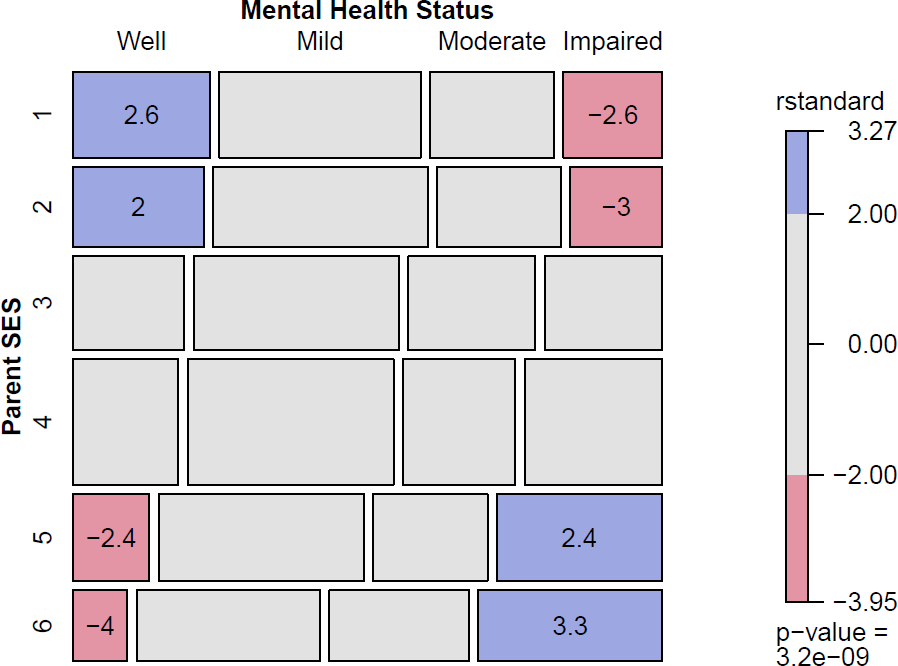
\includegraphics[width=.8\textwidth]{front/fig/mental-plot1} 
% \\
% 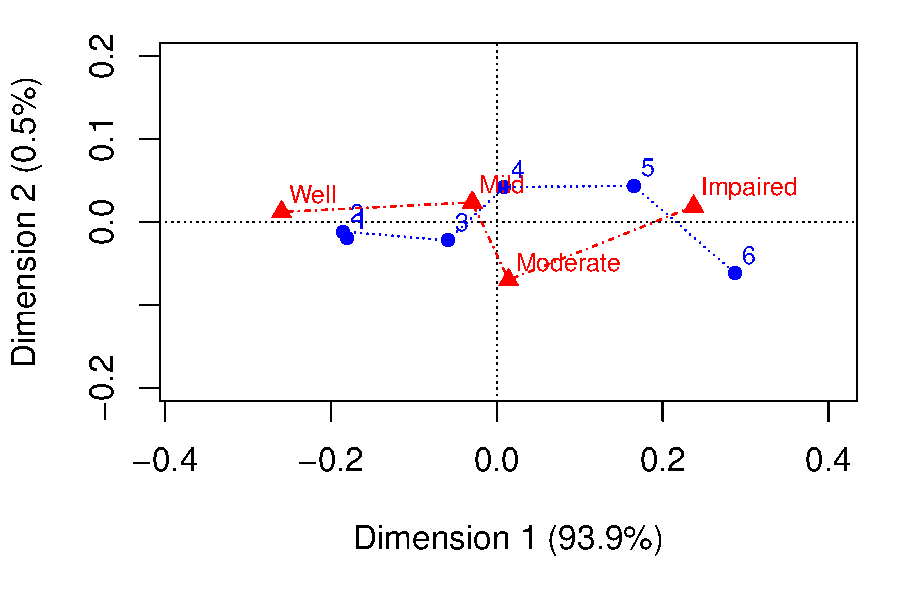
\includegraphics[width=.8\textwidth]{ch06/fig/ca-mental-plot}
}
%\end{titlepage}
\maketitle

%\begin{titlepage}
\title{%
%% simple cover pic for now
\Huge{Visualizing Categorical Data with }

\includegraphics[height=2ex, keepaspectratio]{front/fig/Rlogo}
% below-- use a graphic coverpage
%\input{front/covnew}
%\input{front/covpic}
}
\author{
	{\Large Michael Friendly} \\ York University
	\and
	{\Large David Meyer} \\ UAS Technikum Wien
%	\and
%	with contributions, \\ {\Large Achim Zeilleis} \\ Universit\"at Insbruck
}
\date{\today}
\vspace{1cm}
\titlepic{%
 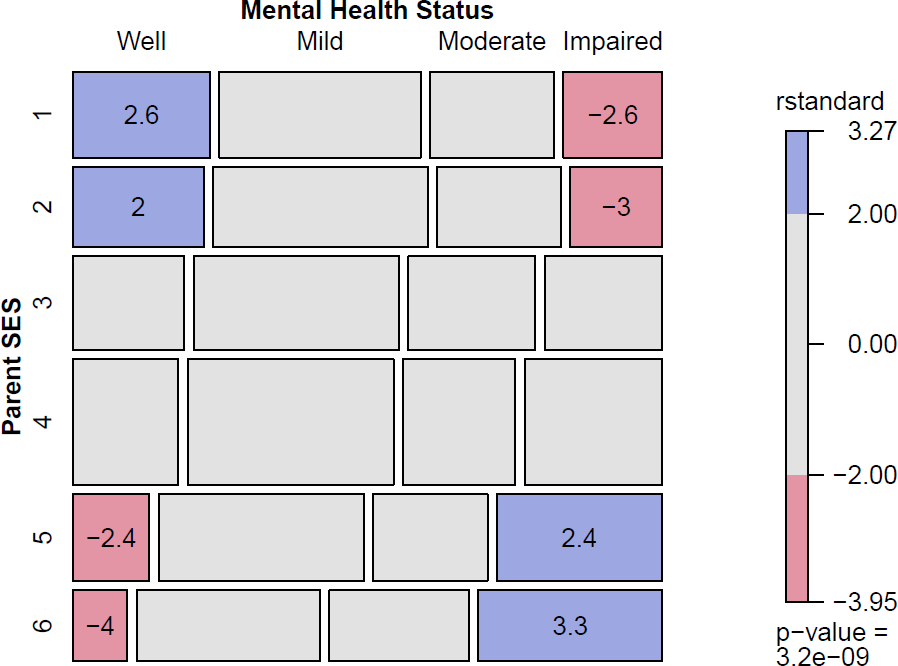
\includegraphics[width=.8\textwidth]{front/fig/mental-plot1} 
% \\
% 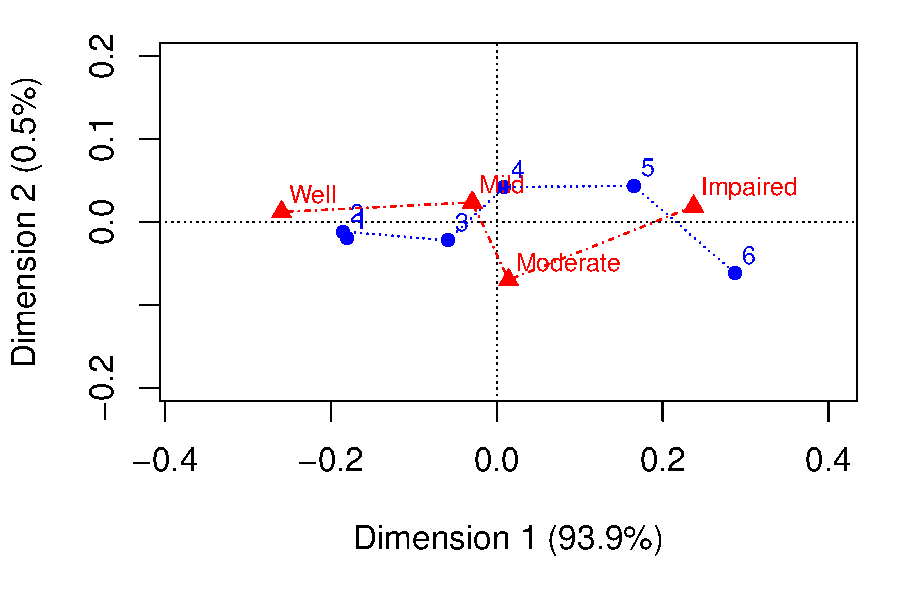
\includegraphics[width=.8\textwidth]{ch06/fig/ca-mental-plot}
}
%\end{titlepage}
\maketitle

%\begin{titlepage}
\title{%
%% simple cover pic for now
\Huge{Visualizing Categorical Data with }

\includegraphics[height=2ex, keepaspectratio]{front/fig/Rlogo}
% below-- use a graphic coverpage
%\input{front/covnew}
%\input{front/covpic}
}
\author{
	{\Large Michael Friendly} \\ York University
	\and
	{\Large David Meyer} \\ UAS Technikum Wien
%	\and
%	with contributions, \\ {\Large Achim Zeilleis} \\ Universit\"at Insbruck
}
\date{\today}
\vspace{1cm}
\titlepic{%
 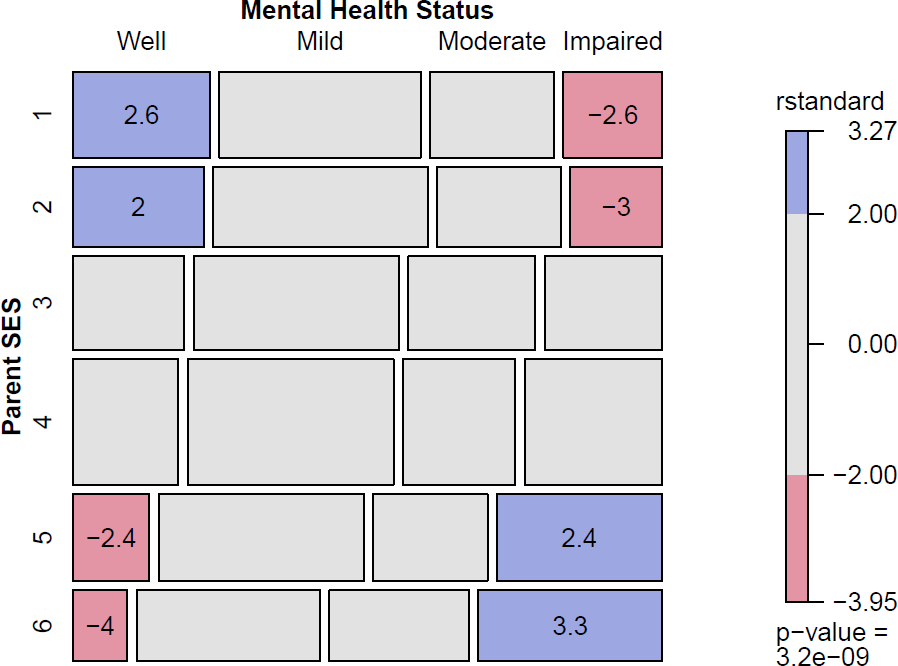
\includegraphics[width=.8\textwidth]{front/fig/mental-plot1} 
% \\
% 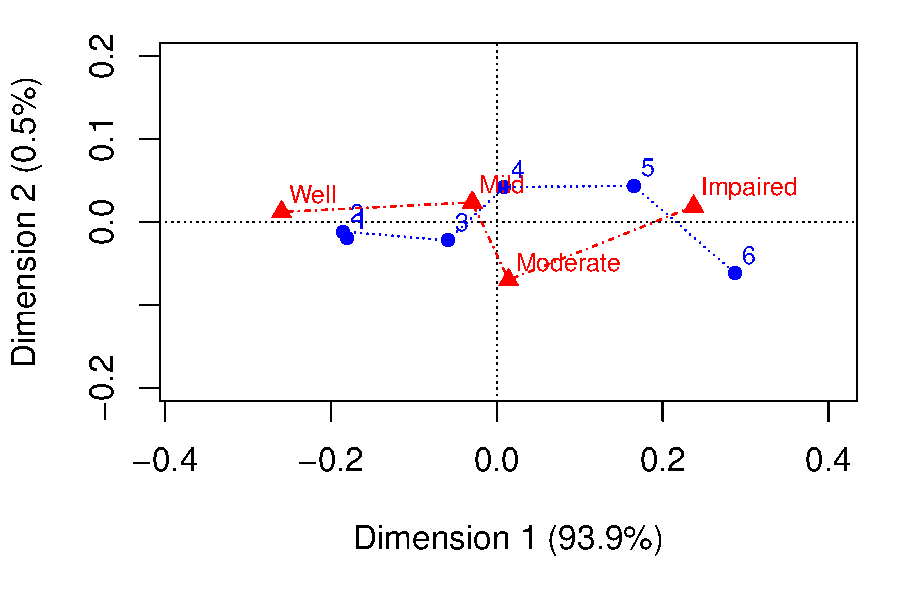
\includegraphics[width=.8\textwidth]{ch06/fig/ca-mental-plot}
}
%\end{titlepage}
\maketitle

\pagenumbering{roman}
%\addcontentsline{toc}{section}{Table of Contents}
{\renewcommand{\baselinestretch}{.8}\normalsize
\tableofcontents
}
%
%{\renewcommand{\baselinestretch}{.75}\normalsize
%\addcontentsline{toc}{section}{List of Tables}
%\listoftables
%}
%%
%{\renewcommand{\baselinestretch}{.75}\normalsize
%\addcontentsline{toc}{section}{List of Figures}
%\listoffigures
%}
%
%{\renewcommand{\baselinestretch}{.75}\normalsize
%\addcontentsline{toc}{section}{List of Outputs}
%\listof{Output}{List of Outputs}
%}
%
%\addtocontents{toc}{\protect\addcontentsline{toc}{section}{Table of Contents}}

\chapter{Preface}
%\addcontentsline{toc}{chapter}{\numberline{}Preface}

\TODO{The preface has not yet been written.  This is just a stub.}

\section*{Audience}
% This book assumes basic understanding of statistical concepts at least at an
% intermediate undergraduate level including regression and analysis of variance
% (for example, at the level of \citet{Neter-etal:90,MendenhallSincich:2003}).
% 
% It is written to appeal to two audiences:
% \begin{itemize*}
%   \item Students and methodologists in the social and health sciences, epidemiology,
%     economics, business
% 	and (bio)statistics
% 	\item Substantive researchers in various disciplines wanting to be able to
% 	apply these methods to their own data
% \end{itemize*}
% 
% It is also assumed that the reader has at least basic knowledge of the \R language and
% environment, including interacting with the \R console (RGui for Windows, R.app for Mac OS X)
% or other graphical user interface (e.g., R Studio), using \R functions in packages,
% getting help for these from \R, etc.  One introductory chapter (\chref{ch:working}) is devoted
% to covering topics beyond such basic skills needed in the book.

\section*{Overview}

\section*{Acknowledgements}


%\chapter{Preface}
%\addcontentsline{toc}{chapter}{\numberline{}Preface}

\TODO{The preface has not yet been written.  This is just a stub.}

\section*{Audience}
% This book assumes basic understanding of statistical concepts at least at an
% intermediate undergraduate level including regression and analysis of variance
% (for example, at the level of \citet{Neter-etal:90,MendenhallSincich:2003}).
% 
% It is written to appeal to two audiences:
% \begin{itemize*}
%   \item Students and methodologists in the social and health sciences, epidemiology,
%     economics, business
% 	and (bio)statistics
% 	\item Substantive researchers in various disciplines wanting to be able to
% 	apply these methods to their own data
% \end{itemize*}
% 
% It is also assumed that the reader has at least basic knowledge of the \R language and
% environment, including interacting with the \R console (RGui for Windows, R.app for Mac OS X)
% or other graphical user interface (e.g., R Studio), using \R functions in packages,
% getting help for these from \R, etc.  One introductory chapter (\chref{ch:working}) is devoted
% to covering topics beyond such basic skills needed in the book.

\section*{Overview}

\section*{Acknowledgements}


%% ============ Main matter ================
\mainmatter
\pagenumbering{arabic}



\chapter{Introduction}\label{ch:intro}
%\begin{center}
 \rule[-4pt]{0.5pt}{4pt}\hrulefill\rule[-4pt]{0.5pt}{4pt}\\
 \begin{minipage}[c]{.33\linewidth}
  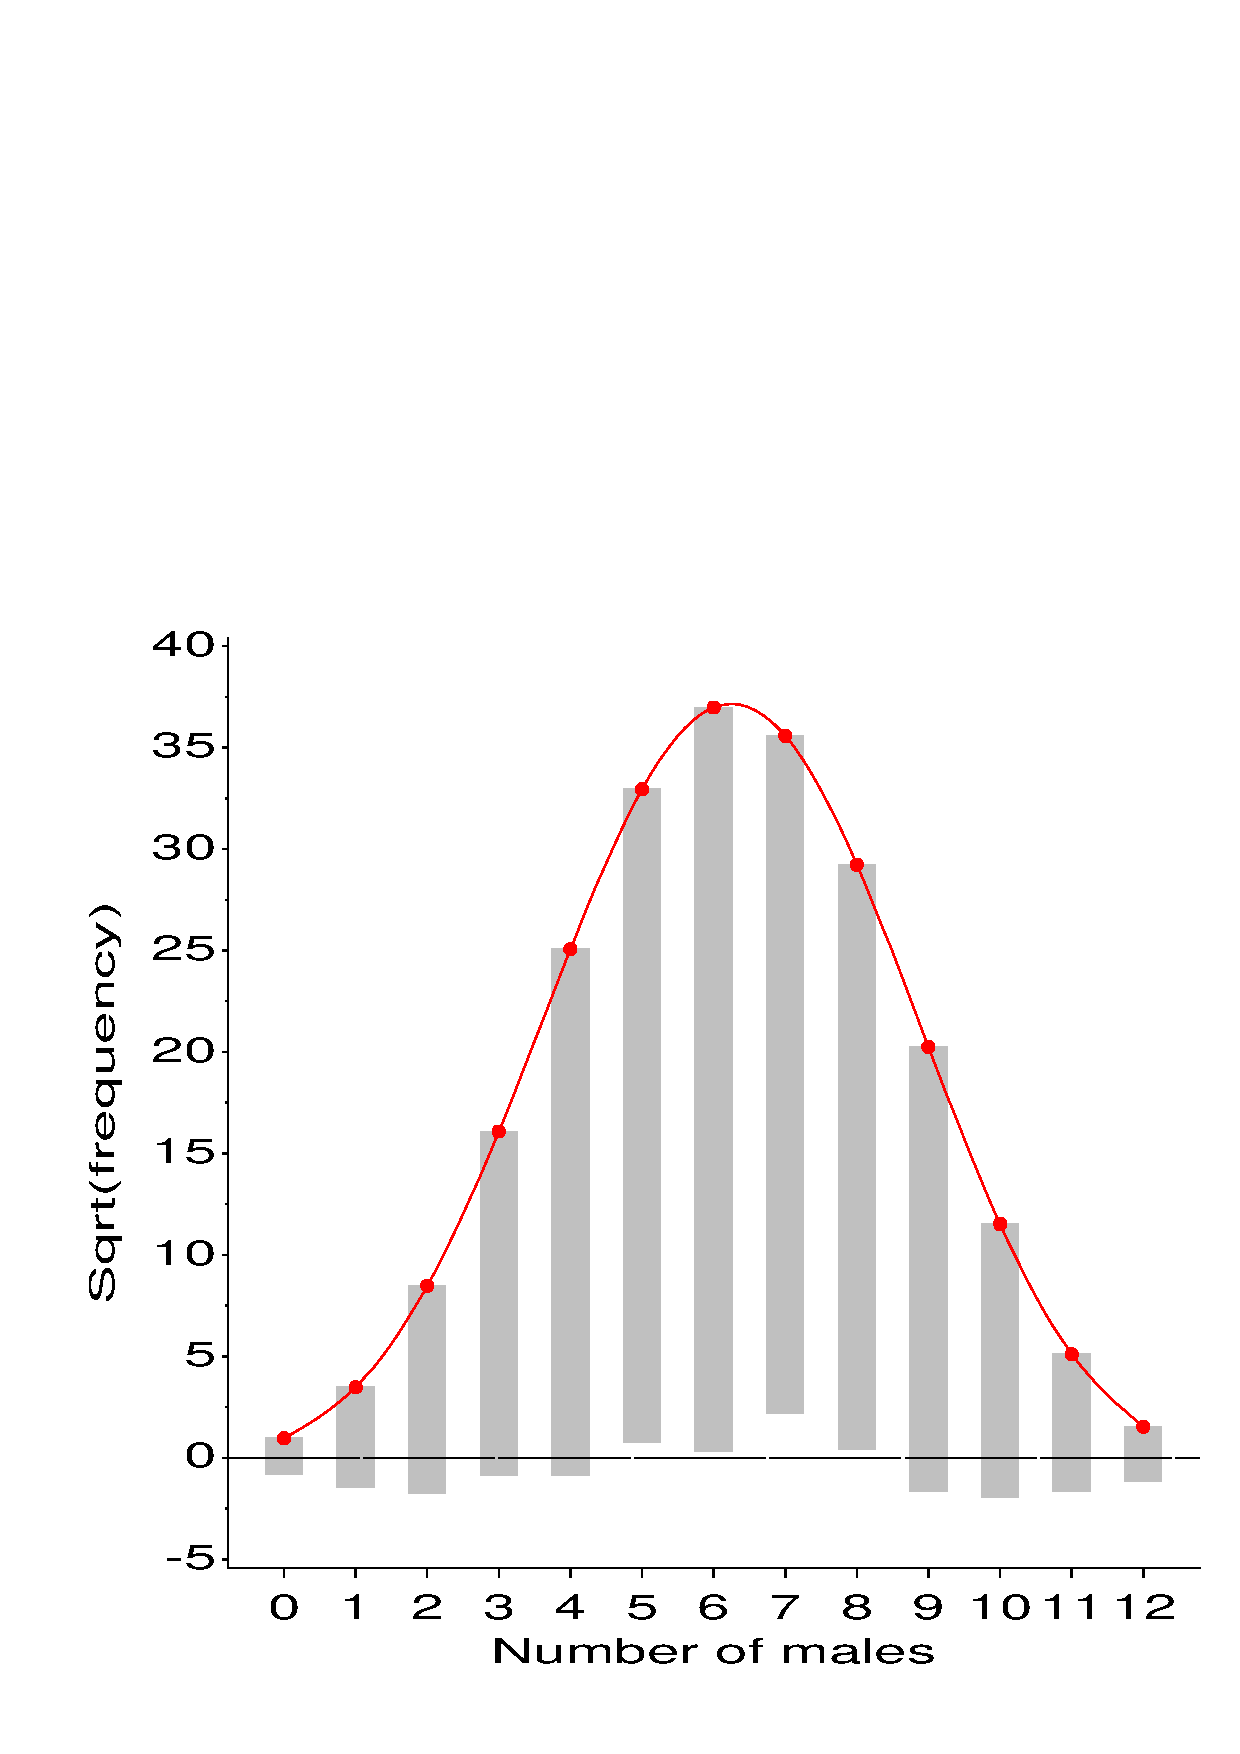
\includegraphics[width=1\linewidth]{saxony}\graphicsfile{ch2/fig/saxony.eps}{}
 \end{minipage}%
 \hfill
 \begin{minipage}[c]{.33\linewidth}
  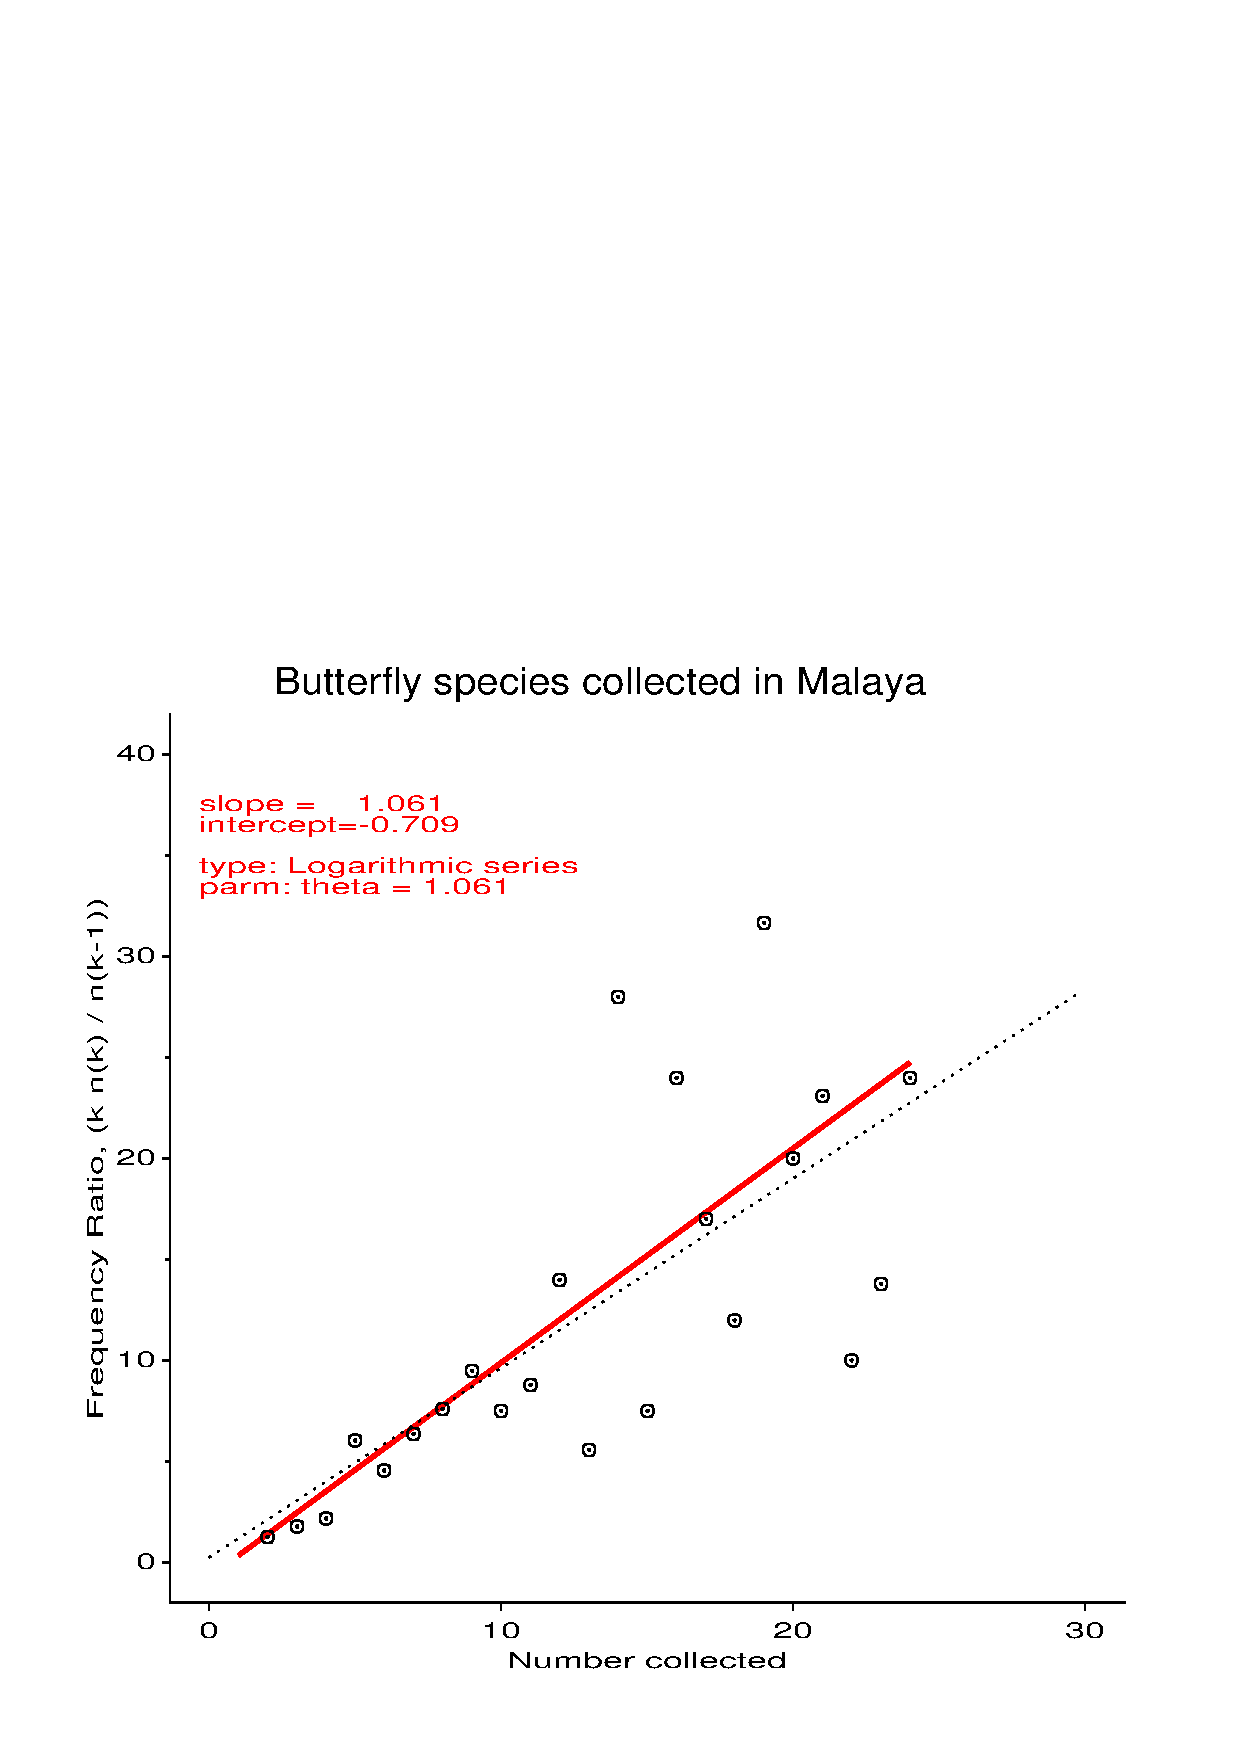
\includegraphics[width=1\linewidth]{orddemo3}\graphicsfile{ch2/fig/orddemo3.eps}{}
 \end{minipage}
 \hfill
 \begin{minipage}[c]{.33\linewidth}
  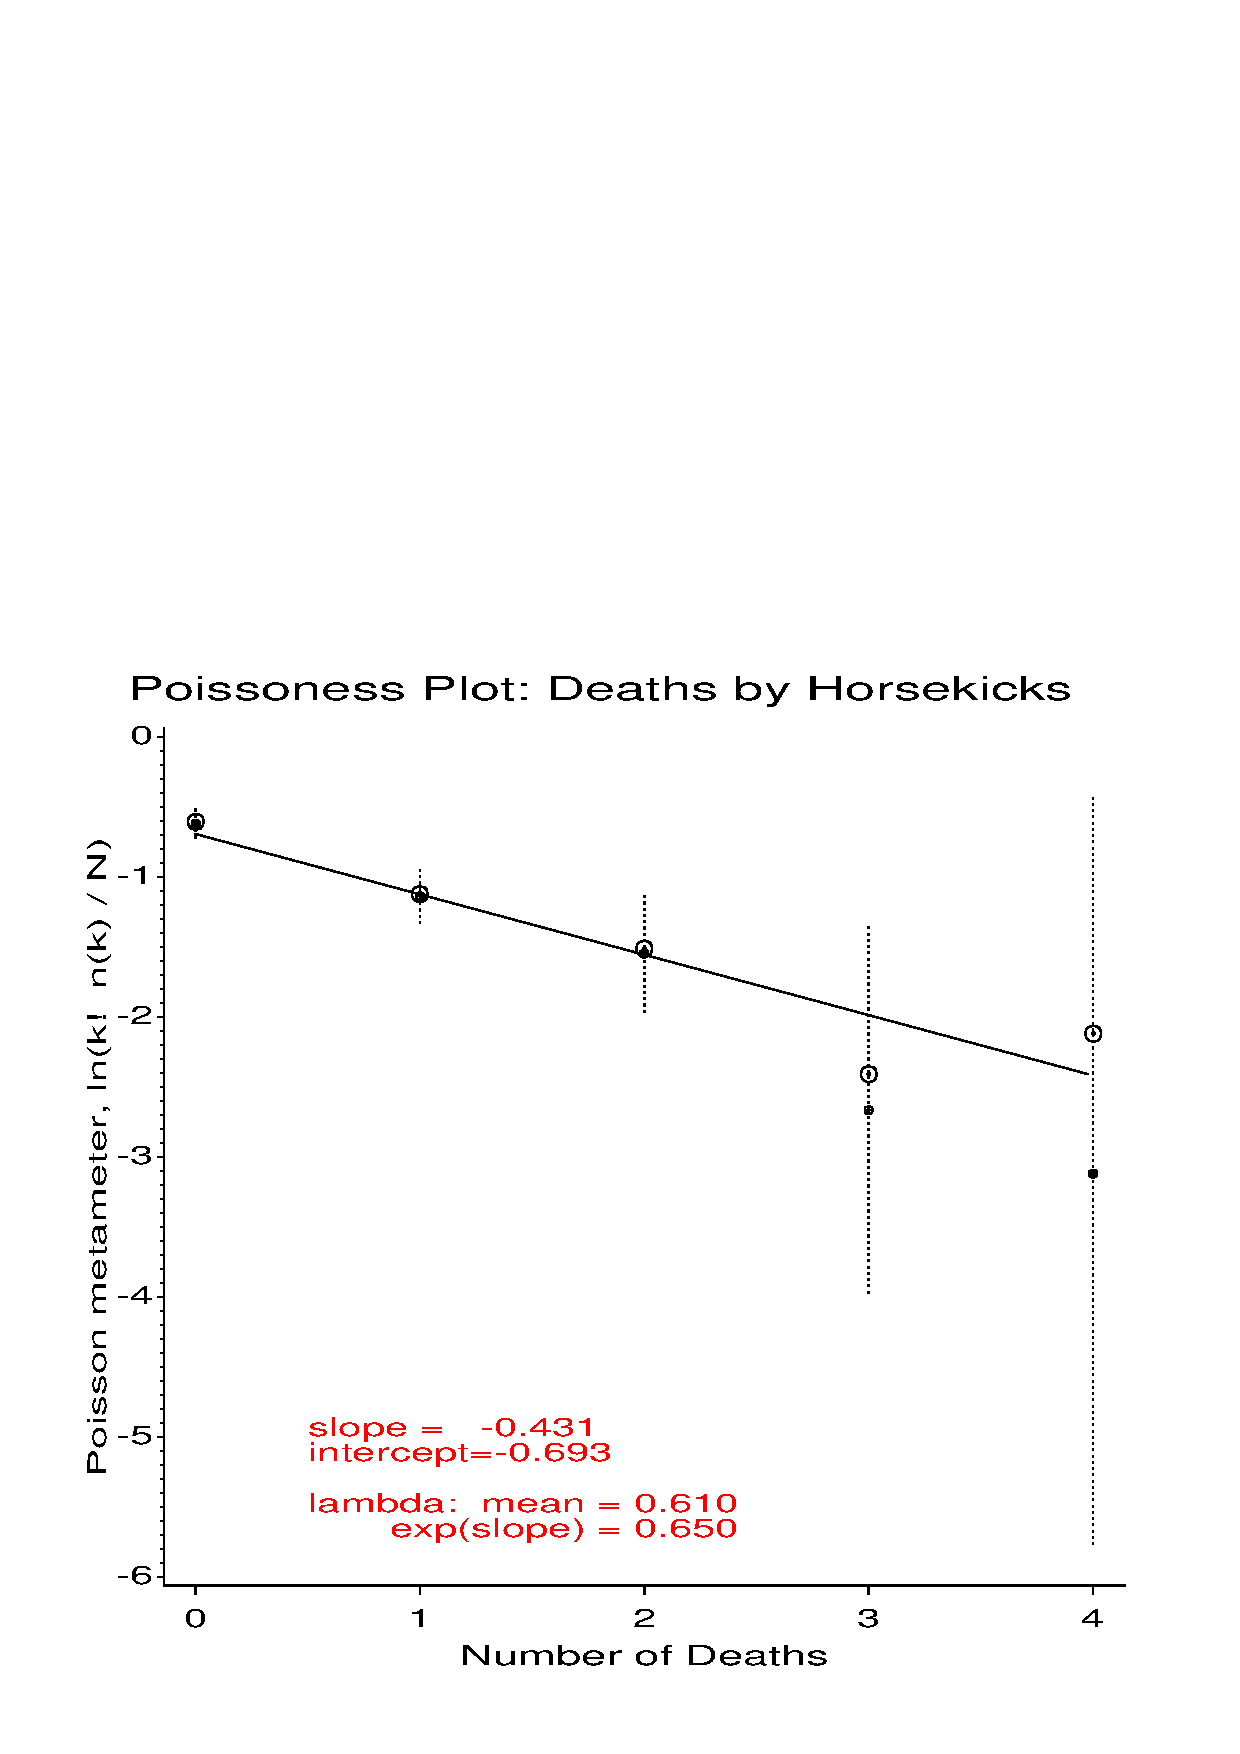
\includegraphics[width=1\linewidth]{poisdemo1}\graphicsfile{ch2/fig/poisdemo1.eps}{}
 \end{minipage}
\end{center}

		% visual table of contents

\chapterprelude{
Categorical data consists of variables whose values comprise a set
of discrete categories.
Such data require different statistical and graphical methods
than commonly used for quantitative data.
The focus of this book is on visualization techniques and graphical
methods designed to reveal patterns of relationships among
categorical variables. This chapter outlines the basic orientation
of the book and some key distinctions regarding the
analysis and visualization of
categorical data.
}
% \minitoc
% \clearpage


\section{Data visualization and categorical data: Overview}\label{sec:viscat}

\epigraph{Beauty is truth; truth, beauty. \\
  That is all ye know on Earth,
  all ye need to know.}{John Keats, \emph{Ode on a Grecian urn}}


``Data visualization'' can mean many things, from popular press
infographics, to maps of voter turnout or party choice.
Here we use this term in the narrower context of statistical
analysis.  As such, we refer to an approach to data analysis that focuses
on \emph{insightful} graphical display in the service of both
\emph{understanding} our data and \emph{communicating} our results to others.

We may display the raw data, some
summary statistics, or some indicators of the quality or adequacy
of a fitted model.  The word ``insightful'' suggests that the goal
is (hopefully) to reveal some aspects of the data which might not
be perceived, appreciated, or absorbed by other means.
As in the quote from Keats, the overall
aims include both beauty and truth, though each of these are
only as perceived by the beholder.

Methods for visualizing quantitative data have a long history
and are now widely used in both data analysis and in data presentation, and
in both popular and scientific media.
Graphical methods for categorical data,
however, have only a more recent history, and are consequently
not as widely used.  The goal of this book is to show concretely how
data visualization may be usefully applied to categorical data.

``Categorical'' data means different things in different
contexts.  We introduce the topic in \secref{sec:whatis}
with some examples illustrating
\begin{seriate}
\item types of categorical variables: binary, nominal, and ordinal,
\item data in case form vs.\ frequency form,
\item frequency data vs.\ count data,
\item univariate, bivariate, and multivariate data, and
\item the distinction between explanatory and response variables.
\end{seriate}

Statistical methods for the analysis of categorical data also fall into two
quite different categories, described and illustrated in \secref{sec:strategies}:
\begin{seriate}
\item the simple randomization-based
methods typified by
the classical Pearson $\chi^2$, Fisher's exact test, and Cochran-Mantel-Haenszel
tests, and
\item the model-based methods represented by
logistic regression, \loglin, and generalized linear models.
\end{seriate}
In this book, \chrange{ch:discrete}{ch:corresp}
are mostly related to the randomization-based methods;
\chrange{ch:logistic}{ch:loglin}
illustrate the model-based methods.

In \secref{sec:methods} we describe some important similarities
and
differences between categorical data and
quantitative data, and discuss the implications of these differences for
visualization techniques.
\secref{sec:vis} outlines a strategy of data analysis
focused on visualization.

In a few cases we show \R code or results as illustrations here,
but the fuller discussion of using \R for categorical data
analysis is postponed to \chref{ch:working}.


\section{What is categorical data?}\label{sec:whatis}

A \term{categorical variable} is one for which the possible measured
or assigned values
consist of a discrete set of categories, which may be \emph{ordered} or
\emph{unordered}.
Some typical examples are:
\begin{itemize*}
\item \var{Gender}, with categories ``Male'', ``Female''.
\item \var{Marital status}, with categories ``Never married'', ``Married'',
``Separated'', ``Divorced'', ``Widowed''.
\item \var{Fielding position} (in baseball), with categories
``Pitcher'', ``Catcher'', ``1st base'', ``2nd base'',  $\dots$, ``Left field''.
\item \var{Side effects} (in a pharmacological study), with categories
``None'', ``Skin rash'', ``Sleep disorder'', ``Anxiety'', $\dots$.
\item \var{Political attitude}, with categories ``Left'', ``Center'', ``Right''.
\item \var{Party preference} (in Canada), with categories ``NDP'', ``Liberal'', ``Conservative'', ``Green''.
\item \var{Treatment outcome}, with categories ``no improvement'', ``some
improvement'', or ``marked improvement''.
\item \var{Age}, with categories ``0-9'', ``10-19'', ``20-29'', ``30-39'',
$\dots$ .
\item \var{Number of children}, with categories $0, 1, 2, \dots$ .
\end{itemize*}

As these examples suggest, categorical variables differ in the number of
categories: we often distinguish
\term{binary variables} such as \var{Gender}
from those with more than two categories (called \term{polytomous variables}).
For example, \tabref{tab:berk220} gives data on 4526 applicants
to graduate departments at the University of California at Berkeley
in 1973, classified by two binary variables, gender and admission status.
\ixe{Berkeley admissions}
\begin{table}[htb]
\caption{Admissions to Berkeley graduate programs}
\label{tab:berk220}
 \begin{center}
\begin{tabular}{lrr|r}
\hline
  & Admitted & Rejected & Total  \\
\hline
 Males & 1198 & 1493 & 2691  \\
 Females & 557 & 1278 & 1835  \\
\hline
 Total & 1755 & 2771 & 4526  \\
\hline
\end{tabular}
\end{center}
\end{table}

Some categorical variables (\var{Political attitude}, \var{Treatment outcome})
may have ordered categories (and are called \term{ordinal}),
while other (\term{nominal}) variables like \var{Marital status}
have unordered categories.%
\footnote{An ordinal variable may be defined as one whose categories are
\emph{unambiguously} ordered along a \emph{single} underlying dimension.
Both marital status and fielding position may be weakly ordered, but
not on a single dimension, and not unambiguously.}
For example, \tabref{tab:arthrit0} shows a $2 \times 2 \times 3$ table of
ordered outcomes (``none'', ``some'' or ``marked'' improvement)
to an active treatment for rheumatoid
arthritis compared to a placebo for men and women.
\ixe{Arthritis treatment}
\begin{table}[tb]

\caption{Arthritis treatment data}\label{tab:arthrit0}
\begin{center}
\begin{tabular}{ll|rrr|r}
\hline
     &  & \multicolumn{3}{c|}{Improvement}            &  \\
\hline
   Treatment&  Sex    &None    &Some    &Marked  &  Total \\[1ex]
\hline
   Active   &  Female &      6 &      5 &     16 &     27 \\
            &  Male   &      7 &      2 &      5 &     14 \\ [0.5ex]
%\hline
   Placebo  &  Female &     19 &      7 &      6 &     32 \\
            &  Male   &     10 &      0 &      1 &     11 \\[1ex]
\hline
   Total    &         &     42 &     14 &     28 &     84 \\
\hline
\end{tabular}
\end{center}
\end{table}



Finally, such variables differ in the
fineness or level to which some underlying observation has been
categorized for a particular purpose.
From one point of view, \emph{all} data
may be considered categorical because the precision of measurement
is necessarily finite, or an inherently continuous variable may be recorded only to limited precision.

But this view is not helpful for the applied
researcher because it neglects the phrase ``for a particular purpose''.
Age, for example, might be treated as a quantitative variable in a study of native language vocabulary, or as an ordered categorical variable
with decade groups (0-10, 11-20, 20-30, $\dots$)
in terms of
the efficacy or side-effects of treatment for depression, or even as a
binary variable (``child'' vs.\  ``adult'') in an analysis of survival following an epidemic or natural disaster. In the analysis of
data using categorical methods, continuous variables are often recoded
into ordered categories with a small set of categories for some purpose.%
\footnote{
This may be wasteful of information available in the original
variable, and should be done for substantive reasons, not mere
convenience.  For example, some researchers unfamiliar with
regression methods often perform a ``median-split'' on
quantitative predictors
so they can use ANOVA methods. Doing this precludes the possibility
of determining if those variables have non-linear relations with
the outcome.
}

\subsection{Case form vs.\ frequency form}\label{sec:case-freq}
In many circumstances, data is recorded on each individual or experimental
unit.  Data in this form is called case data,
or data in \term{case form}.
The data in \tabref{tab:arthrit0}, for example, were derived from
the individual data listed in the data set \data{Arthritis}
from the \Rpackage{vcd}.  The following lines show the first
five  of $N=84$ cases in the \data{Arthritis} data,
\begin{knitrout}
\definecolor{shadecolor}{rgb}{1, 0.961, 0.933}\color{fgcolor}\begin{kframe}
\begin{alltt}
\hlkwd{data}\hlstd{(}\hlstr{"Arthritis"}\hlstd{,} \hlkwc{package}\hlstd{=}\hlstr{"vcd"}\hlstd{)}
\hlkwd{head}\hlstd{(Arthritis,} \hlnum{5}\hlstd{)}
\end{alltt}
\begin{verbatim}
##   ID Treatment  Sex Age Improved
## 1 57   Treated Male  27     Some
## 2 46   Treated Male  29     None
## 3 77   Treated Male  30     None
## 4 17   Treated Male  32   Marked
## 5 36   Treated Male  46   Marked
\end{verbatim}
\end{kframe}
\end{knitrout}

Whether or not the data variables, and the questions we ask, call for
categorical or quantitative data analysis,
when the data are in case form,
we can always trace
any observation back to its individual identifier or data record
(for example, if the case with \code{ID==57} turns out to be unusual
or noteworthy).

Data in \term{frequency form}
has already been tabulated, by counting over the categories of the
table variables. The same data shown as a table in
\tabref{tab:arthrit0} appear in frequency form as shown below.
\begin{knitrout}
\definecolor{shadecolor}{rgb}{1, 0.961, 0.933}\color{fgcolor}\begin{kframe}
\begin{alltt}
\hlkwd{as.data.frame}\hlstd{(}\hlkwd{xtabs}\hlstd{(}\hlopt{~}\hlstd{Treatment}\hlopt{+}\hlstd{Sex}\hlopt{+}\hlstd{Improved,} \hlkwc{data}\hlstd{=Arthritis))}
\end{alltt}
\begin{verbatim}
##    Treatment    Sex Improved Freq
## 1    Placebo Female     None   19
## 2    Treated Female     None    6
## 3    Placebo   Male     None   10
## 4    Treated   Male     None    7
## 5    Placebo Female     Some    7
## 6    Treated Female     Some    5
## 7    Placebo   Male     Some    0
## 8    Treated   Male     Some    2
## 9    Placebo Female   Marked    6
## 10   Treated Female   Marked   16
## 11   Placebo   Male   Marked    1
## 12   Treated   Male   Marked    5
\end{verbatim}
\end{kframe}
\end{knitrout}

Data in frequency form may be analyzed by methods
for quantitative data if there is a quantitative response variable
(weighting each group by the cell frequency, with a \code{weight}
variable).
Otherwise, such data are generally
best analyzed by methods for categorical data, where
statistical models are often expressed as models for the
frequency variable, in the form of an \R formula
like \verb|Freq ~ .|.

In any case, an observation in a data set in
frequency form refers
to all cases in the cell collectively, and these cannot be identified individually.
Data in case form can always be reduced to frequency form,
but the reverse is rarely possible. In \chref{ch:working},
we identify a third format, \term{table form}, which is the
\R representation of a table like \tabref{tab:arthrit0}.

\subsection{Frequency data vs.\ count data}\label{sec:freq-count}
In many cases the observations represent the classifications of events or variables are
recorded from \emph{operationally independent} experimental units or individuals, typically
a sample from some population.  The tabulated data may be called
\term{frequency data}.  The data in \tabref{tab:berk220} and \tabref{tab:arthrit0}
are both examples of frequency data because each observation tabulated
comes from a different person.

However, if several events or variables are observed for the same units or individuals, those events are not
operationally independent, and it is useful to use the term
\term{count data} in this situation.  These terms (following
\citet{Lindsey:95}) are by no means standard, but
the distinction is often important, particularly in statistical
models for categorical data.

For example, in a tabulation of the number of male
children within families (\tabref{tab:saxdata}, described in
\secref{sec:uni-multi} below),
the number of male children in a given family would be a \emph{count} variable,
taking values $0, 1, 2, \dots$.  The number of independent families with
a given number of male children is a \emph{frequency} variable.
Count data also arise when we tabulate a sequence of events over time
or under different circumstances in a number of individuals.

\ixe{Families in Saxony}
\begin{table}[htb]
 \caption{Number of Males in 6115 Saxony Families of Size 12}\label{tab:saxdata}
 \begin{center}
 \begin{tabular}{lrrrrrrrrrrrrr}
  \hline
  Males & 0 & 1 & 2 & 3 & 4 & 5 & 6 & 7 & 8 & 9 & 10 & 11 & 12 \\ 
  Families & ~~~3 & ~~24 & ~104 & ~286 & ~670 & 1033 & 1343 & 1112 & ~829 & ~478 & 181 & ~~45 & ~~~7 \\ 
  \hline
 \end{tabular}
 \end{center}
\end{table}


\subsection{Univariate, bivariate, and multivariate data}\label{sec:uni-multi}
Another distinction concerns the number of variables: one, two or
(potentially) many shown in a data set or table, or used in some
analysis.
\tabref{tab:berk220} is an example of a bivariate (two-way) \ctab
and \tabref{tab:arthrit0} classifies the observations by three variables.
Yet, we will see later
that the Berkeley admissions data also recorded
the department to which potential students applied (giving a three-way
table), and in the arthritis data, the age of subjects was also
recorded.

Any \ctab (in frequency or table form) therefore records the \emph{marginal totals}, summed over all
variables not represented in the table.
For data in case form, this means simply ignoring (or not recording)
one or more variables;  the ``observations'' remain the same.
Data in frequency form, however, result in smaller tables when
any variable is ignored;  the ``observations'' are the cells of
the \ctab. For example, in the \data{Arthritis} data, ignoring \var{Sex}
gives the smaller $2 \times 3$ table for \var{Treatment} and \var{Improved}.
\begin{knitrout}
\definecolor{shadecolor}{rgb}{1, 0.961, 0.933}\color{fgcolor}\begin{kframe}
\begin{alltt}
\hlkwd{as.data.frame}\hlstd{(}\hlkwd{xtabs}\hlstd{(}\hlopt{~}\hlstd{Treatment} \hlopt{+} \hlstd{Improved,} \hlkwc{data}\hlstd{=Arthritis))}
\end{alltt}
\begin{verbatim}
##   Treatment Improved Freq
## 1   Placebo     None   29
## 2   Treated     None   13
## 3   Placebo     Some    7
## 4   Treated     Some    7
## 5   Placebo   Marked    7
## 6   Treated   Marked   21
\end{verbatim}
\end{kframe}
\end{knitrout}


In the limiting case, only one table variable may be recorded or
available, giving the categorical equivalent of univariate data.
For example, \tabref{tab:saxdata} gives data on the distribution
of the number of male children in families with 12 children
(discussed further in \exref{ex:saxony1}).
These data were part of a large tabulation of the sex distribution
of families in Saxony in the 19$^{th}$ century, but the data in \tabref{tab:saxdata}
have only one discrete classification variable, number of males.
Without further information, the only statistical questions concern
the form of the distribution.
We discuss methods for fitting and graphing such discrete distributions
in \chref{ch:discrete}.
The remaining chapters relate to bivariate and multivariate data.
\ixe{Families in Saxony}


\subsection{Explanatory vs.\ Response variables}\label{sec:exp-resp}
\ix{variable!response \~|(}
Most statistical models make a distinction between \term{response variables}
(or \emph{dependent}, or \emph{criterion} variables)
and
\term{explanatory variables}
(or \emph{independent}, or \emph{predictor} variables).

In the standard (classical) linear models for regression and analysis of variance
(ANOVA), for instance, we treat one (or more) variables as responses,
to be explained by the other, explanatory variables.
The explanatory variables may be quantitative or categorical
(e.g., factors in \R).
This affects only the details of how the model is specified
or how coefficients are interpreted for
\func{lm} or \func{glm}.  In these classical models,
the response variable (``treatment outcome'', for example), must be
considered quantitative,  and the model attempts to describe how the
\emph{mean} of the distribution of responses changes with the values
or levels of the explanatory variables, such as age or gender.

However, when the response variable is categorical, however, the standard linear
models do not apply, because they assume a normal (Gaussian) distribution
for the model residuals.  For example, in \tabref{tab:arthrit0}
the response variable
is \var{Improvement}, and even if numerical scores were assigned
to the categories ``none'', ``some'', ``marked'', it may be unlikely
that the assumptions of the classical linear models could be met.

Hence, a categorical \emph{response} variable generally requires analysis
using methods for categorical data, but categorical \emph{explanatory} variables
may be readily handled by either method.

The distinction between response and explanatory variables also
becomes important in the use of \loglin models for frequency tables
(described in \chref{ch:loglin}), where models can be specified
in a simpler way (as equivalent logit models) by focusing on the response
variable.
\ix{variable!response \~|)}


\section{Strategies for categorical data analysis}\label{sec:strategies}

Methods of analysis for categorical data can be classified into two
broad categories:
those concerned with hypothesis testing \emph{per se}, and those concerned with model building.

\subsection{Hypothesis testing approaches}\label{sec:strategies-hyp}
In many studies, the questions of substantive interest translate readily
into questions concerning hypotheses about \term{association} between variables, a more general idea than that of correlation
(\emph{linear} association) for quantitative variables.
If a non-zero association exists, we may wish to characterize the
strength of the association numerically and understand the pattern or
nature of the association.

For example, in \tabref{tab:berk220}, a main question is:
``Is there evidence of gender-bias in admission to graduate school?''
Another way to frame this: ``Are males more likely to be admitted?''
These questions can
be expressed in terms of an association between gender and
admission status in a $2 \times 2$ \ctab\
of applicants classified by these two variables.
If there is evidence for an association, we can assess its strength by a variety of
measures, including the difference in proportions admitted for men
and women or the ratio of the odds of admission for men compared to
women, as described in \secref{sec:twoway-twobytwo}.

Similarly, in \tabref{tab:arthrit0}, questions about the efficacy of the
treatment for rheumatoid arthritis can be answered in terms of
hypotheses about the associations among the table variables:
\var{Treatment}, \var{Sex}, and the \var{Improvement} categories.
Although the main concern might be focused on the overall association between
Treatment and Improvement, one would also wish to know if this association
is the same for men and women.
A \term{stratified analysis} (\secref{sec:twoway-strat}) controls for the effects of background
variables like Sex, and tests for \term{homogeneity of association}
help determine if these associations are equal.

Questions involving tests of such hypotheses are answered most easily
using a large variety of specific statistical tests, often based on
randomization arguments.
These include the familiar Pearson chi-square test for two-way tables,
the Cochran-Mantel-Haenszel test statistics, Fisher's exact test, and a wide range of measures of strength of association.
These tests make minimal assumptions, principally requiring that subjects
or experimental units have been randomly assigned to the categories of
experimental factors.  The hypothesis testing approach is illustrated
in \chref{ch:twoway}--\ref{ch:corresp}, though the emphasis is on graphical
methods which help to understand the nature of association between
variables.

\begin{Example}[haireye0]{Hair color and eye color}
%\begin{table}[htb]

\caption{Hair-color eye-color data}\label{tab:hairdat}
\begin{center}
\begin{tabular}{|lrrrr|r|}
\hline
        & \multicolumn{4}{c|}{Hair Color}        & \\
Eye     &         &         &         &         &       \\
Color   &  Black  &  Brown  &    Red  &  Blond  & Total \\[2ex] \hline
Green   &      5  &     29  &     14  &     16  &    64 \\
Hazel   &     15  &     54  &     14  &     10  &    93 \\
Blue    &     20  &     84  &     17  &     94  &   215 \\
Brown   &     68  &    119  &     26  &      7  &   220 \\[1ex] \hline
Total   &    108  &    286  &     71  &    127  &   592 \\ \hline
\end{tabular}
\end{center}
\end{table}


%\tabref{tab:hairdat}
The data \data{HairEye} below
records data on the the relationship between hair color and eye color
in a sample of nearly 600 students.
\begin{knitrout}
\definecolor{shadecolor}{rgb}{1, 0.961, 0.933}\color{fgcolor}\begin{kframe}
\begin{alltt}
\hlkwd{library}\hlstd{(vcd)}
\hlstd{(HairEye} \hlkwb{<-} \hlkwd{margin.table}\hlstd{(HairEyeColor,} \hlkwd{c}\hlstd{(}\hlnum{1}\hlstd{,} \hlnum{2}\hlstd{)))}
\end{alltt}
\begin{verbatim}
##        Eye
## Hair    Brown Blue Hazel Green
##   Black    68   20    15     5
##   Brown   119   84    54    29
##   Red      26   17    14    14
##   Blond     7   94    10    16
\end{verbatim}
\end{kframe}
\end{knitrout}

The standard analysis (with \func{chisq.test} or \func{assocstats})
gives a
Pearson \(\chi^2\) of 138.3 with nine degrees of freedom,
indicating substantial departure from independence.  Among the measures of
strength of association, the \term{phi coefficient},
$\phi = \sqrt{\chi^2 / N} = 0.483$, indicates a substantial relationship
between hair and eye color.

\begin{knitrout}
\definecolor{shadecolor}{rgb}{1, 0.961, 0.933}\color{fgcolor}\begin{kframe}
\begin{alltt}
\hlkwd{assocstats}\hlstd{(HairEye)}
\end{alltt}
\begin{verbatim}
##                     X^2 df P(> X^2)
## Likelihood Ratio 146.44  9        0
## Pearson          138.29  9        0
## 
## Phi-Coefficient   : 0.483 
## Contingency Coeff.: 0.435 
## Cramer's V        : 0.279
\end{verbatim}
\end{kframe}
\end{knitrout}
The further (and perhaps more interesting question) is how do we
understand the \emph{nature} of this association between hair
and eye color?
Two graphical methods related to the hypothesis testing approach
are shown in \figref{fig:haireye02}.

\begin{knitrout}
\definecolor{shadecolor}{rgb}{1, 0.961, 0.933}\color{fgcolor}\begin{figure}[!htbp]


\centerline{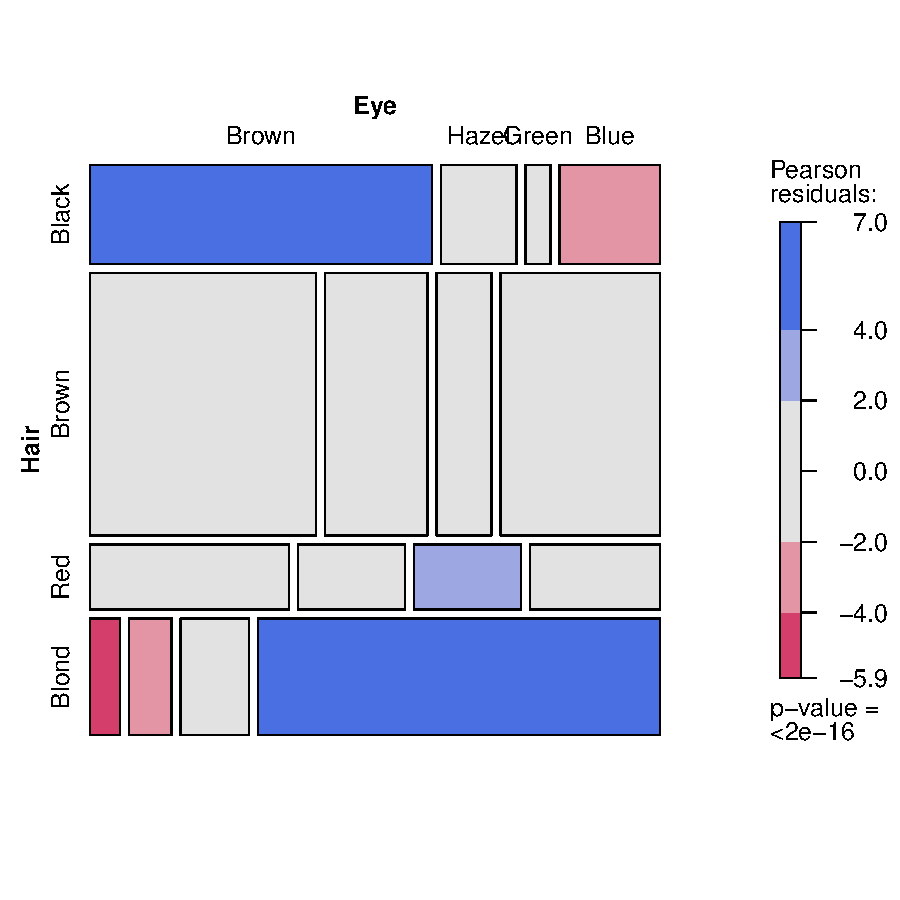
\includegraphics[width=.49\textwidth]{ch01/fig/haireye02-1} 
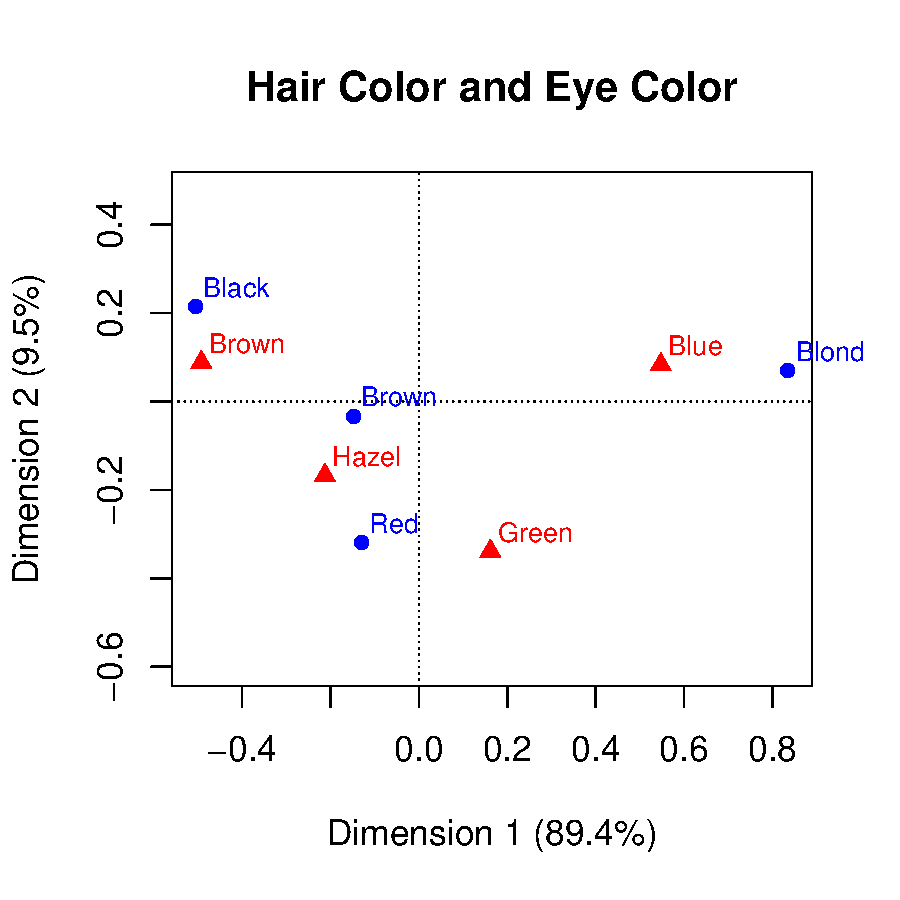
\includegraphics[width=.49\textwidth]{ch01/fig/haireye02-2} }

\caption[Graphical displays for the hair color and eye color data]{Graphical displays for the hair color and eye color data. Left: mosaic display; right: correspondence analysis plot\label{fig:haireye02}}
\end{figure}


\end{knitrout}
The left panel of \figref{fig:haireye02} is a \term{mosaic display}
(\chref{ch:mosaic}), constructed so that the size of each rectangle
is proportional to the observed cell frequency. The shading
reflects the cell contribution to the \(\chi^2\) statistic---shades of blue
when the observed frequency is substantially greater than the
expected frequency under independence, shades of red when the observed frequency
is substantially less, as shown in the legend.

The right panel of this figure shows the results of
a \ca (\chref{ch:corresp}), where the deviations of the hair color and eye
color points from the origin accounts for as much of the \(\chi^2\)
as possible in two dimensions.

We observe that both the hair colors and the eye colors
are ordered from dark to light in the mosaic display and along
Dimension 1 in the \ca plot.  The deviations between observed
and expected frequencies have an opposite-corner pattern in the
mosaic display, except for the combination of red hair and green
eyes, which also stand out as the largest values on Dimension 2
in the \CA plot.
Displays such as these provide a means to understand \emph{how}
the variables are related.
\end{Example}

\subsection{Model building approaches}
Model-based methods provide tests of equivalent
hypotheses about associations, but
offer additional advantages (at the cost of additional assumptions)
not provided by the simpler hypotheses-testing approaches.
Among these advantages, model-based methods provide estimates,
standard errors and confidence intervals for parameters, and the
ability to obtain predicted (fitted) values with associated measures
of precision.

We illustrate this approach here for a dichotomous response variable,
where it is often convenient to
construct a model relating a function of the probability, $\pi$,
of one event to a linear combination of the explanatory variables.
Logistic regression uses the \term{logit function},
\begin{equation*}
 \logit ( \pi ) \equiv \log_e \left( \frac { \pi } {1 - \pi} \right)
\end{equation*}
which may be interpreted as the \term{log odds} of the given event.
A linear logistic model
can then be expressed as
\begin{equation*}
 \logit ( \pi ) = \beta_0 + \beta_1 x_1 + \beta_2 x_2 + \dots
\end{equation*}

Statistical inferences from model-based methods provide tests of
hypotheses for the effects of the predictors, $x_1, x_2, \dots$,
but they also provide estimates of parameters in the model,
$\beta_1, \beta_2, \dots$ and associated confidence intervals.
Standard modeling tools allow us to graphically display the
fitted response surface (with confidence or prediction intervals)
and even to extrapolate these predictions beyond the given data.
A particular advantage of the logit represent ion
in the logistic regression model is that estimates of odds ratios
(\secref{sec:twoway-odds})
may be obtained directly from the parameter estimates.

\begin{Example}[nasa0]{Space shuttle disaster}
\ixd{Space shuttle disaster|(}
To illustrate the model-based approach,
the graph in \figref{fig:spaceshuttle0} is based on
a logistic regression model predicting the probability of a
failure in one of the O-ring seals used in the 24 NASA space shuttles
prior to the disastrous launch of the
\emph{Challenger} in January, 1986.  The explanatory variable is the ambient temperature at the time of the flight.
The sad story behind these data, and the lessons to be learned for
graphical data display are related in \exref{ex:nasa}.

\begin{knitrout}
\definecolor{shadecolor}{rgb}{1, 0.961, 0.933}\color{fgcolor}\begin{figure}[!htbp]


\centerline{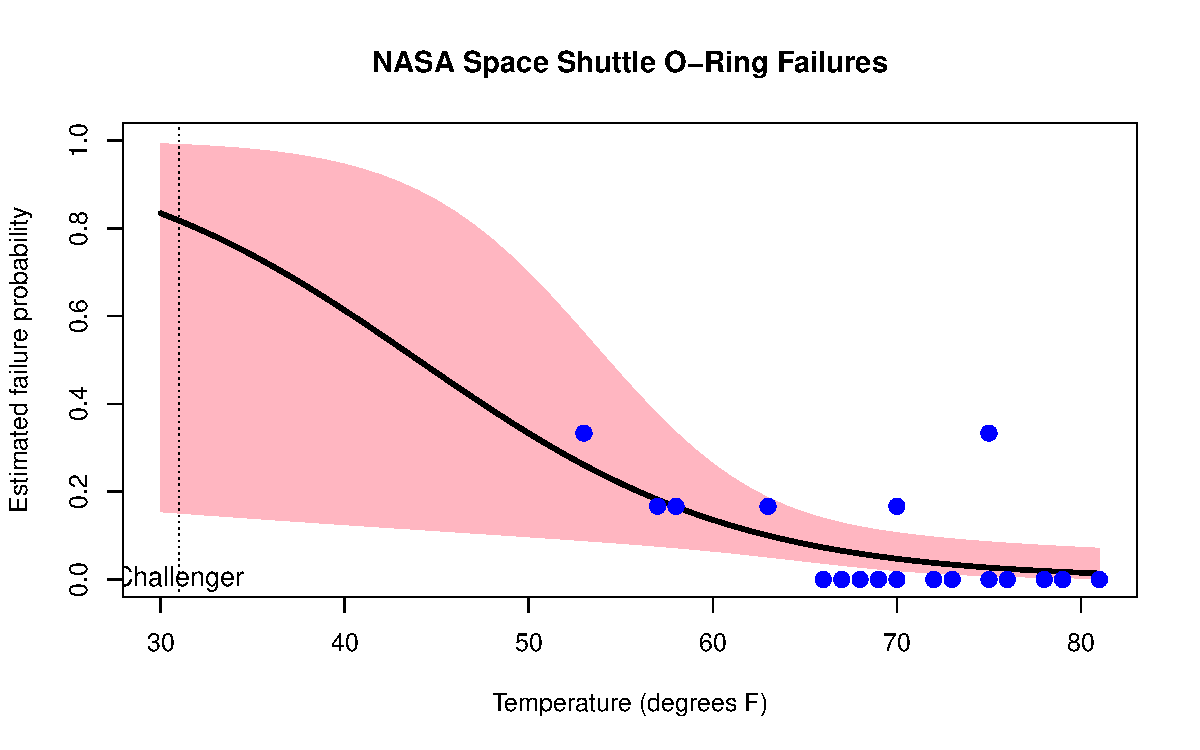
\includegraphics[width=.7\textwidth]{ch01/fig/spaceshuttle0-1} }

\caption[Space shuttle O-ring failure, observed and predicted probabilities]{Space shuttle O-ring failure, observed and predicted probabilities. The dotted vertical line at \degree{31} shows the prediction for the launch of the \emph{Challenger}.\label{fig:spaceshuttle0}}
\end{figure}


\end{knitrout}

Here, we simply note that the fitted model, shown by the solid line in
\figref{fig:spaceshuttle0}, corresponds to the prediction equation
(with standard errors shown in parentheses),
\begin{equation*}
 \logit ( \mbox{Failure} ) =  \cwe{5.09}{3.06} - \cwe{0.116}{0.047} \mbox{ Temperature}
 \end{equation*}%
A hypothesis test that failure probability is unassociated with temperature
is equivalent to the test that the coefficient for temperature in this
model equals 0; this test has a $p$-value of 0.014, convincing evidence
for rejection.

The parameter estimate for temperature, $-0.116$, however, gives more information.  Each \degree{1} increase in temperature decreases the log odds
of failure by 0.116, with 95\% confidence interval ($-0.208$, $-0.0235$).  The equivalent odds ratio is $\exp(-0.116) = 0.891$ (0.812--0.977).
Equivalently, a \degree{10} \emph{decrease} in temperature corresponds to
an odds ratio of a failure of
$\exp(10 \times 0.116) = 3.18$, more than tripling the odds of a failure.

When the \emph{Challenger} was launched, the temperature was only \degree{31}.
The shaded region in \figref{fig:spaceshuttle0} show 95\% prediction intervals
for failure probability.  All previous shuttles (shown by the points
in the figure) had been launched at much warmer temperatures, so the
prediction interval (the dashed vertical line)
at \degree{31} represents a considerable extrapolation
beyond the available data.  Nonetheless, the model building approach
does provide such predictions along with measures of their uncertainty.
\figref{fig:spaceshuttle0} is a graph
that might have saved lives.

\ixd{Space shuttle disaster|)}
\end{Example}

%\TODO{Perhaps replace this example with a similar one for the \code{Donner} data}

\begin{Example}[donner0]{Donner Party}
In April--May of 1846 (three years before the California gold rush),
the Donner and Reed families set out for California from the American mid-west
in a wagon train to seek a new life and perhaps their fortune in the new
American frontier.
By mid July, a large group had reached a site
in present-day Wyoming;  George Donner was elected to lead what was
to be called the ``Donner Party,'' which eventually numbered 87 people
in 23 wagons, along with their oxen, cattle, horses, and worldly possessions.

They were determined to reach California as quickly as possible.
Lansford Hastings, a self-proclaimed trailblazer (retrospectively,
of dubious distinction), proposed that the party follow him through
a shorter path through the Wasatch Mountains.  Their choice
of ``Hastings's Cutoff'' proved disastrous: Hastings had never
actually crossed that route himself, and the winter of of 1846 was to
be one of the worst on record.

In October, 1846, heavy snow stranded them in the eastern Sierra
Nevada, just to the east of a pass which bears their name today.
The party made numerous attempts to seek rescue, most turned back
by blizzard conditions. Relief parties in March--April 1847 rescued
40, but discovered grizzly evidence that those who survived had
cannibalized those who died.

Here we briefly examine of how statistical models and
graphical evidence can shed light on the question of
who survived in the Donner party.

\begin{knitrout}
\definecolor{shadecolor}{rgb}{1, 0.961, 0.933}\color{fgcolor}\begin{figure}[!htbp]


\centerline{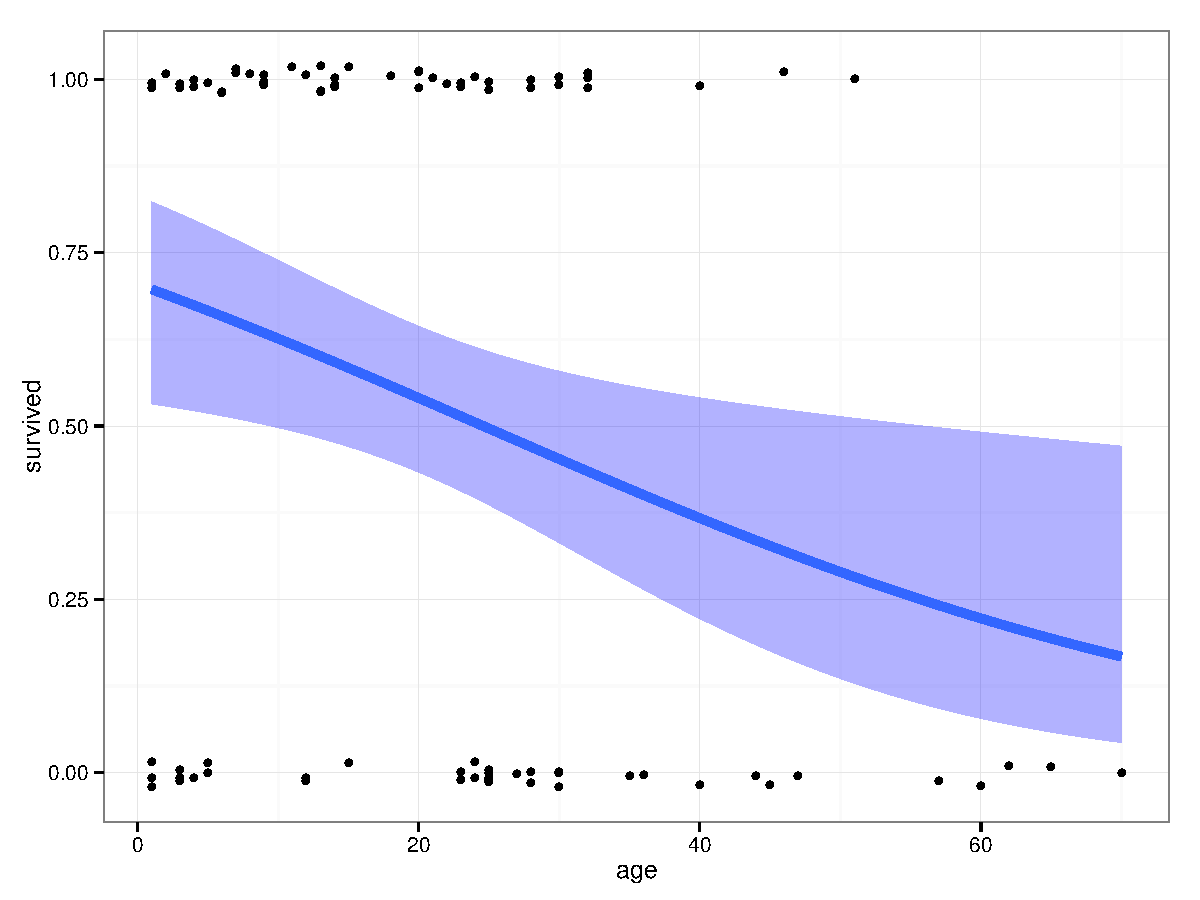
\includegraphics[width=.7\textwidth]{ch01/fig/donner0-1} }

\caption[Donner party data, showing the relationship between age and survival]{Donner party data, showing the relationship between age and survival. The blue curve and confidence band give the predicted probability of survival from a linear logistic regression model.\label{fig:donner0}}
\end{figure}


\end{knitrout}

\figref{fig:donner0} is an example of what we call a \emph{data-centric, model-based}
graph of a discrete (binary) outcome: lived (1) versus died (0). That is, it shows
both the data and a statistical summary based on a fitted statistical model.
The statistical model provides a smoothing of the discrete data.

The jittered points at the top and bottom of the graph show survival in relation
to age of the person.  You can see that there were more people who survived
among the young, and more who died among the old.
The blue curve in the plot shows the fitted probability of survival from
a linear logistic regression model for these data with a 95\% confidence band
for that predictions.  The prediction equation for this model can
be given as:

\begin{equation*}
 \logit ( \mbox{survived} ) =  \cwe{0.868}{0.372} - \cwe{0.0353}{0.015} \mbox{ age}
 \end{equation*}

 It implies that the log odds of survival decreases by 0.0352 with each additional year of
 age or by $10 \times 0.0352 = 0.352$ for an additional decade.
 Another way to say this is that the odds of survival is multiplied by
 $\exp({0.353}) = .702$ with each 10 years of age, a 30\% decrease.

 Of course, these visual and statistical summary depends on the validity of fitted model.
 For contrast, \figref{fig:donner0-other} shows two other model-based smoothers that
 relax the assumption of the linear logistic regression model.
 The left panel shows the result of fitting a semi-parametric model with a
 natural cubic spline with one more degree of freedom than the linear
 logistic model.  The right panel shows the fitted curve for a non-parametric,
 loess model.  Both of these hint that the relationship of survival to age is
 more complex than what is captured in the linear logistic regression model.
 We return to these data in \chref{ch:logistic}.


\begin{knitrout}
\definecolor{shadecolor}{rgb}{1, 0.961, 0.933}\color{fgcolor}\begin{figure}[!htbp]


\centerline{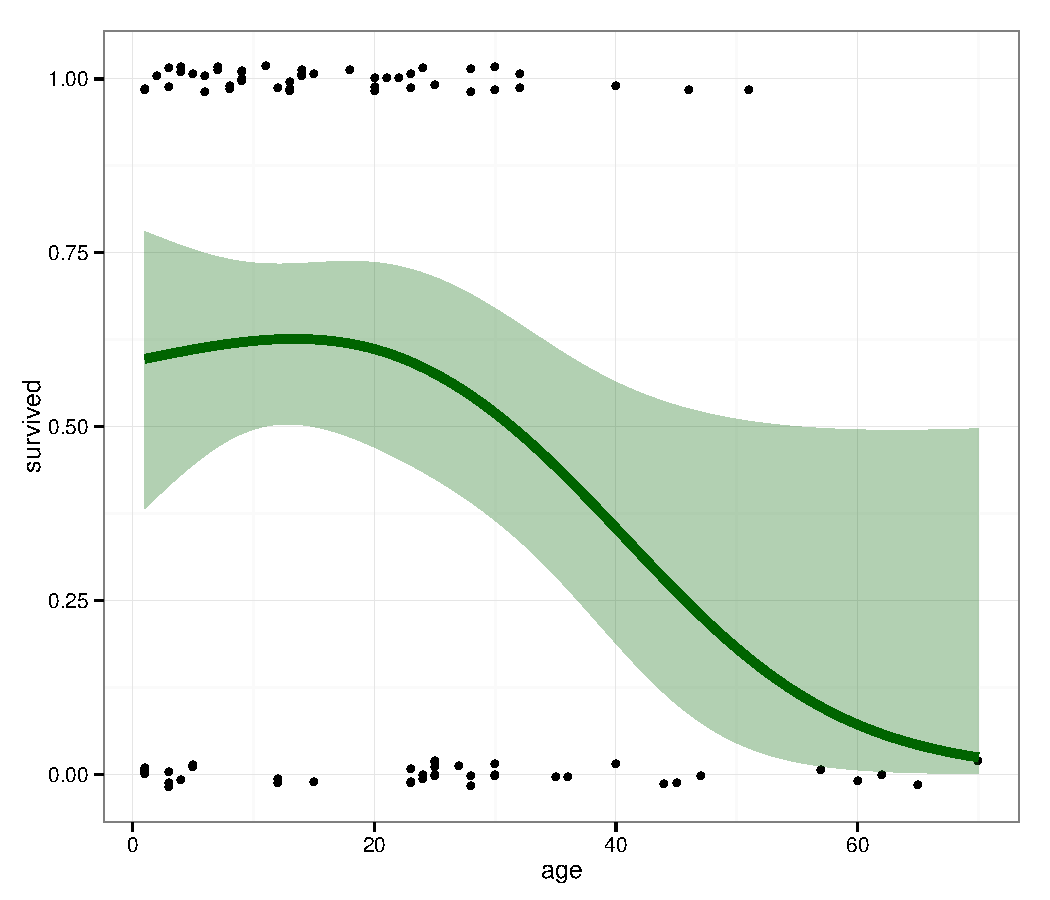
\includegraphics[width=.49\textwidth]{ch01/fig/donner0-other-1} 
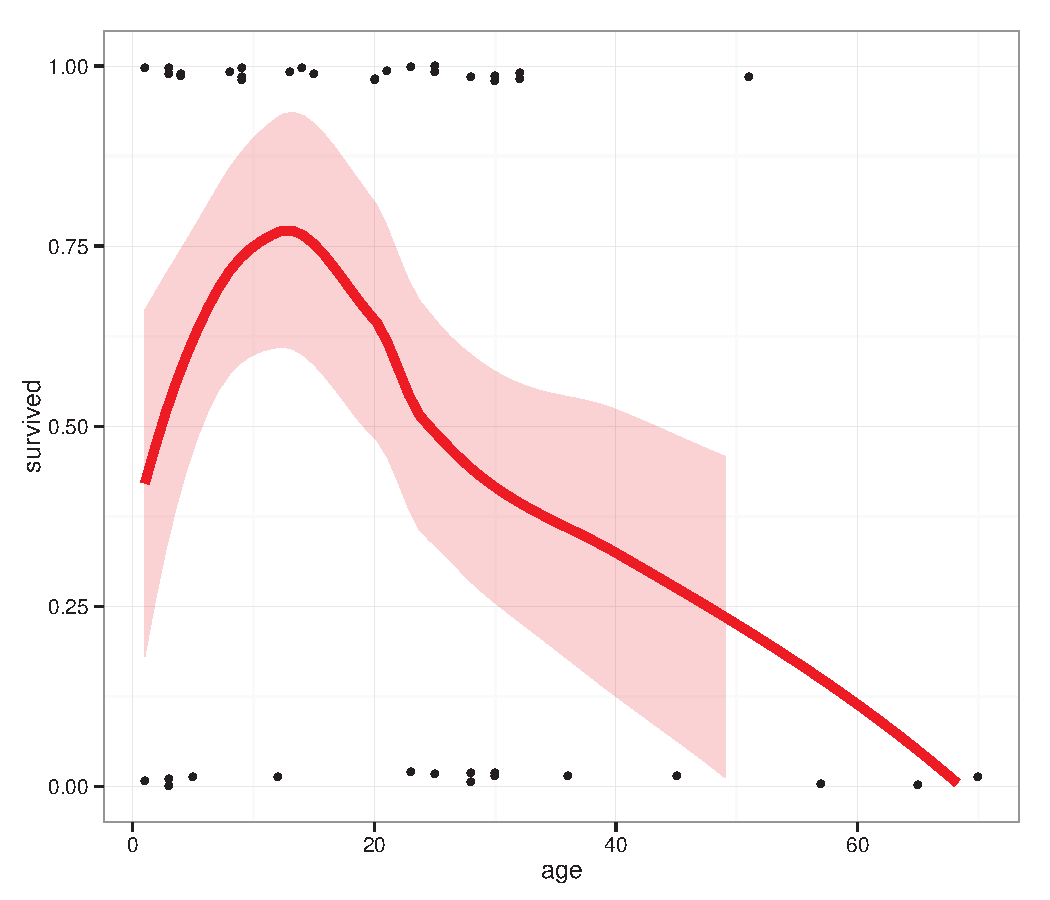
\includegraphics[width=.49\textwidth]{ch01/fig/donner0-other-2} }

\caption[Donner party data, showing other model-based smoothers for the relationship between age and survival]{Donner party data, showing other model-based smoothers for the relationship between age and survival. Left: using a natural spline; right: using a non-parametric loess smoother.\label{fig:donner0-other}}
\end{figure}


\end{knitrout}

%\TODO{Complete this example}
\end{Example}

\section{Graphical methods for categorical data}\label{sec:methods}

\epigraph{You can see a lot, just by looking}{Yogi Berra}

The graphical methods for categorical data described in this book
are in some cases straightforward adaptations of more familiar
visualization techniques developed for quantitative data.
Graphical principles and strategies, and the relations between
the visualization approach and traditional statistical methods
are described in a number of sources, including
\citet{Chambers-etal:83},
\citet{Cleveland:VisData} and several influential books by Tufte
\citep{Tufte:83,Tufte:90,Tufte:97,Tufte:2006}.

The fundamental ideas of statistical graphics as a comprehensive system
of visual signs and symbols with a grammar and semantics was first proposed
in Jacques Bertin's \emph{Semiology of Graphics} \citeyearpar{Bertin:83},
These ideas were later extended to a computational theory
in Wilkinson's \emph{Grammar of Graphics} \citeyearpar{Wilkinson:2005},
and implemented in \R in Hadley Wickham's \Rpackage{ggplot2}
\citep{Wickham:2009:ggplot2,ggplot2}.

Another perspective on visual data display is presented in \secref{sec:intro-goals}
focusing on the communication goals of statistical graphics.
However, the discrete nature of categorical data implies that
some familiar graphic methods need to be adapted, while in other
cases we require a new graphic metaphor for data display.
These issues are illustrated in \secref{sec:intro-catdata}.
\secref{sec:effect-order} discusses the principle of effect ordering
for categorical variables in graphs and tables.

\subsection{Goals and design principles for visual data display}\label{sec:intro-goals}

Designing good graphics is surely an art, but as surely, it is
one that ought to be informed by science.
In constructing a graph, quantitative and qualitative information is
encoded by visual features, such as position, size, texture, symbols
and color. This translation is reversed when a person studies a
graph. The representation of numerical magnitude and categorical
grouping, and the apperception of patterns and their \emph{meaning} must be extracted from the visual display.

There are many views of graphs, of graphical perception, and of
the roles of data visualization in discovering and communicating
information.
On the one hand, one may regard a graphical display as a \emph{stimulus}---
a package of information to be conveyed to an idealized observer.
From this perspective certain questions are of interest:  which
form or graphic aspect promotes greater accuracy or speed of judgment
(for a particular task or question)?  What aspects lead to greatest
memorability or impact?
Cleveland \citep{ClevelandMcGill:84b,ClevelandMcGill:85,Cleveland:93:JCGS},
Spence and Lewandowsky
\citep{LewandowskySpence:89,Spence:90,SpenceLewandowsky:90} have made important contributions to our understanding of
these aspects of graphical display.

An alternative view regards a graphical display as an act
of \emph{communication}---like a narrative, or even a poetic text or work of art.
This perspective places the greatest emphasis on the desired
communication goal, and judges the effectiveness of a graphical
display in how well that goal is achieved \citep{FriendlyKwan:2011}.
\citet{Kosslyn:85,Kosslyn:89} and \citet{Tufte:83,Tufte:90,Tufte:97}
have articulated this perspective most clearly.

In this view,
an effective graphical display, like good writing, requires an
understanding of its \emph{purpose}---what aspects of the data are to be
communicated to the viewer.  In writing we communicate most
effectively when we know our audience and tailor the message
appropriately. So too, we may construct a graph in different ways to:
\begin{seriate}
  \item use ourselves,
  \item present at a conference or meeting of our colleagues,
  \item publish in a research report, or
  \item communicate to a general audience
\end{seriate}
(\citet[Ch. 1]{Friendly:91}, \citet{FriendlyKwan:2011}).
\figref{fig:presentation-exploration} illustrates a basic contrast between graphs
for presentation purposes, designed to appeal persuasively to a large audience
(one-to-many)
and the use of perhaps many graphs we might make for ourselves for
exploratory data analysis (many-to-one).
% \citep{Unwin:99}.

\begin{figure}[htb]
\centering
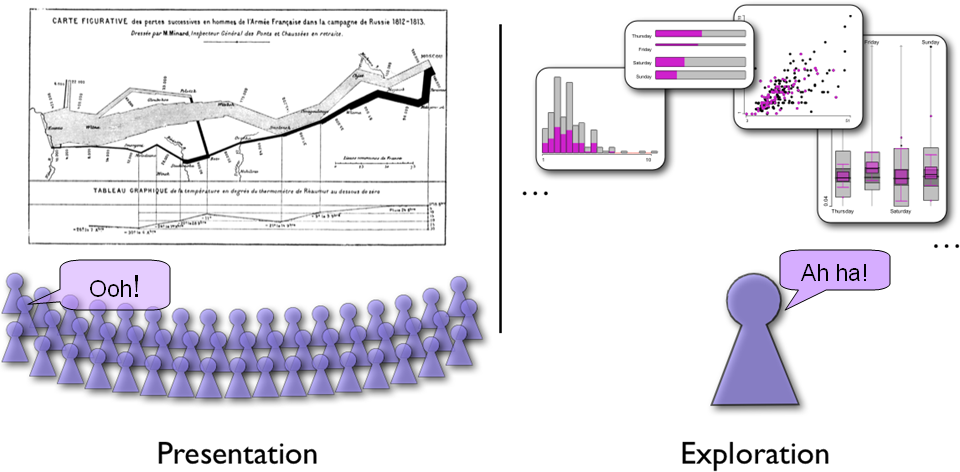
\includegraphics[width=.8\textwidth]{ch01/fig/presentation-exploration2}
\caption[Different communication purposes require different graphs]{Different communication purposes require different graphs. For presentations, a single, carefully crafted graph may appeal best to a large audience; for exploratory analysis, many related images from different perspectives for a narrow audience (often you!). \emph{Source}: Adapted from a blog entry by Martin Theus, \url{http://www.theusrus.de/blog/presentation-vs-exploration/}.}\label{fig:presentation-exploration}
\end{figure}

\figref{fig:datadisp}
shows one organization of visualization methods in terms
of the \emph{primary} use or intended communication goal,
the functional \emph{presentation goal}, and suggested corresponding
\emph{design principles}.
\begin{figure}[htbp]
  \centering
  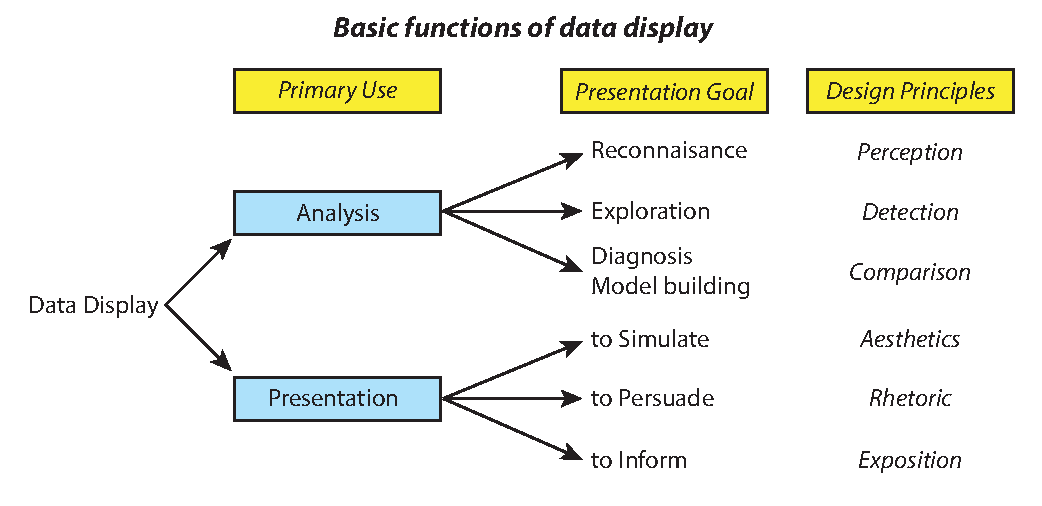
\includegraphics[width=\textwidth]{ch01/fig/datadisp}
  \caption[Basic functions of data display]{A taxonomy of the basic functions of data display by intended use, presentation goal and design principles.}\label{fig:datadisp}
\end{figure}

We illustrate these ideas and distinction in the examples below, most of which
are treated again in later chapters.

\begin{Example}[arrests0]{Racial profiling: Arrests for marijuana possession}
In a case study that will be examined in detail in \chref{ch:logistic} (\exref{ex:arrests}),
the \emph{Toronto Star} newspaper studied a huge data base of arrest records by
Toronto police for indications of possible racial profiling, i.e., differential
treatment of those arrested on the basis of skin color.
They focused on the charge of simple possession of a small amount of marijuana,
for which enforcement procedures allowed police discretion.  An officer could
release an arrestee with a summons (``Form 9'') to appear in court,
or take the person to a police station for questioning (``Form 10'') or
booking (``Form 11.1'') or order the person held in jail for a bail hearing (``Show cause'').

The statistical issue was whether the data on these arrests showed evidence of differential
treatment in relation to skin color, particularly in the treatment of blacks vs. whites,
controlling, of course, for other factors. Statistical tests on these data
(\chisq tests, loglinear models, logistic regression) showed overwhelming evidence of
differential treatment of blacks and whites. However, tables of these results do not
reveal the nature of this association.

\figref{fig:arrests0-mosaic} is an example of
a graph designed for \emph{analysis}--- a mosaic display (\chref{ch:mosaic})
showing the frequencies of those arrested
on this charge by skin color and release type.  The size of each rectangle shows the
frequency and these are shaded in relation to the asociation between skin color and
release--- blue for positive associations (more than expected under independence) to
red for negative associations.
\begin{figure}[htb]
\centering
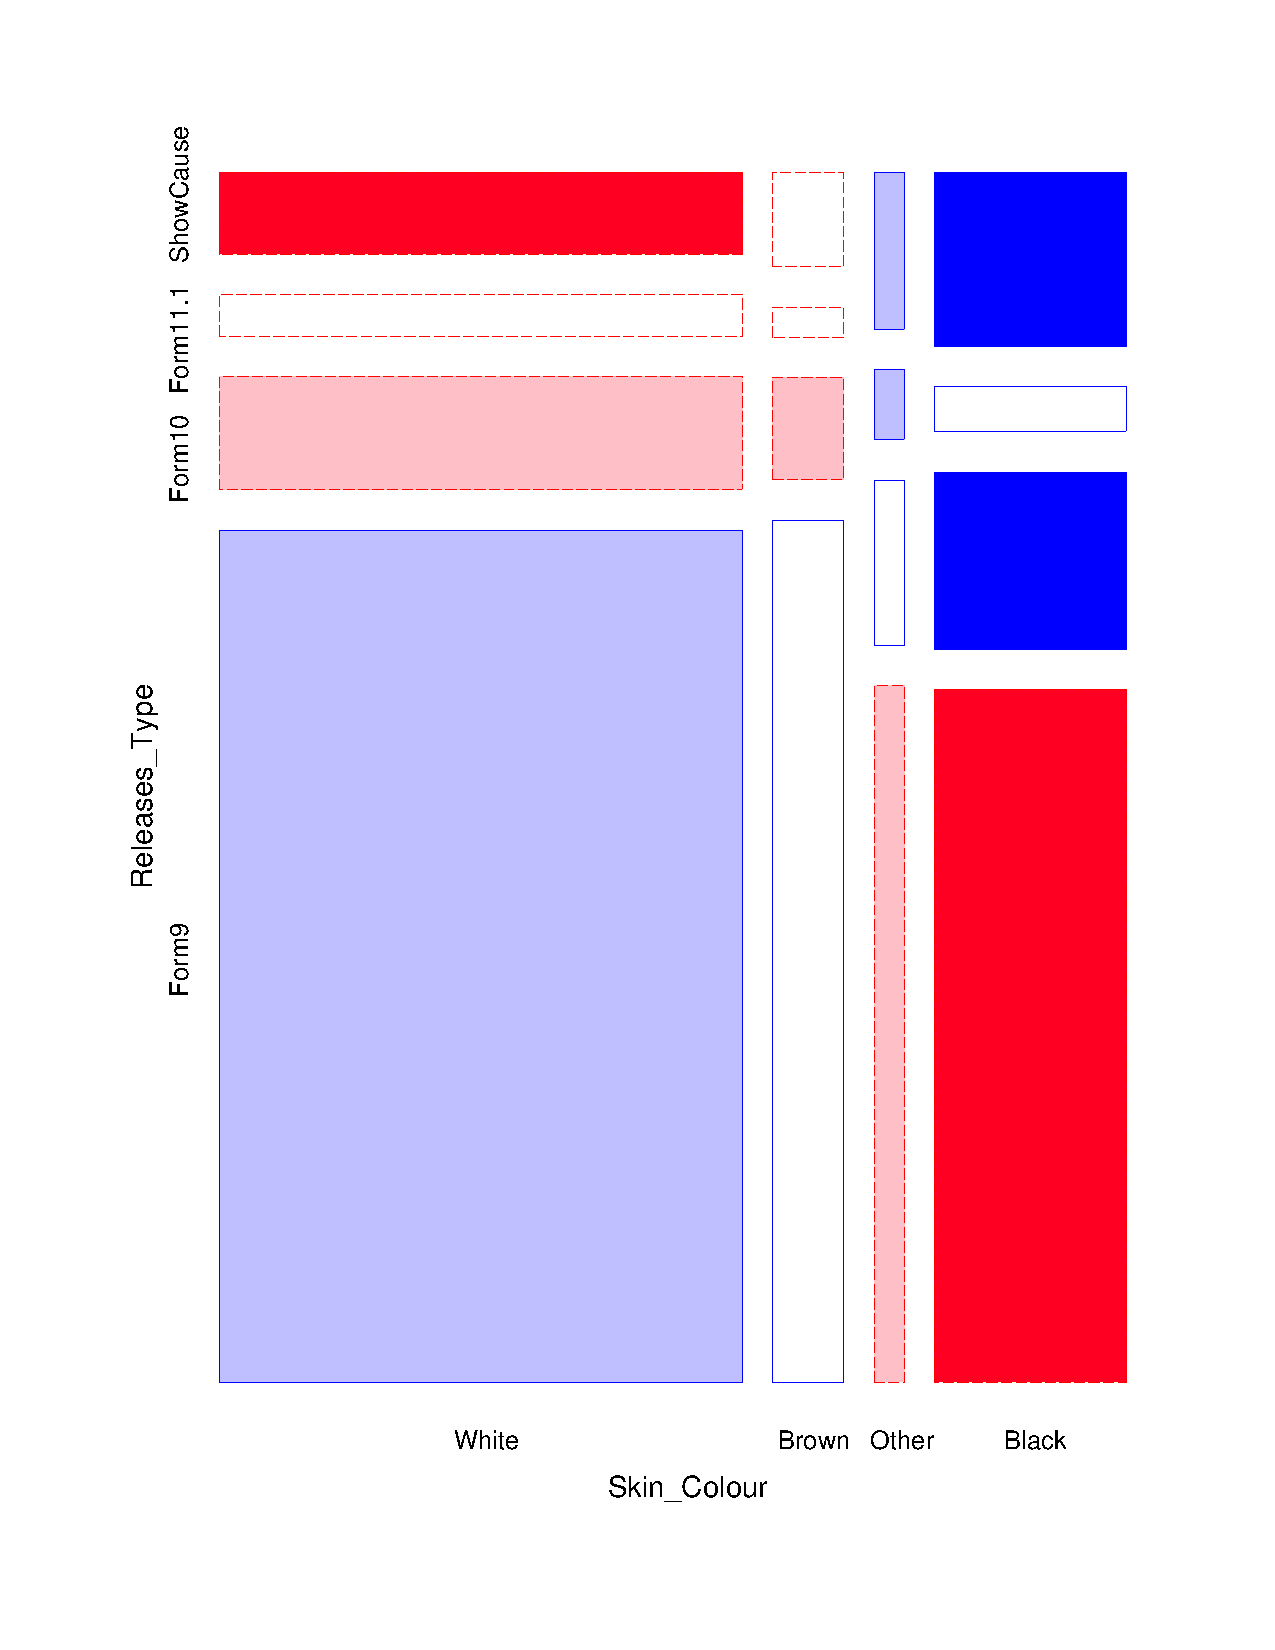
\includegraphics[width=.5\textwidth]{ch01/fig/arrests-skin-color}
\caption{Mosaic display showing the relationship between skin color and release type for those arrested on a charge of simple possession of marijuana in Toronto, 1996-2002.}\label{fig:arrests0-mosaic}
\end{figure}

Once you know how to read such graphs, the pattern is clear: blacks were indeed more likely
to be held for more severe treatment, whites were more likely to be released with a
summons.  But this is hardly a graph that would be clear to a general audience,
and would require a good deal of explanation.

In contrast, \figref{fig:arrests0-star} shows a redesign of this as a \emph{presentation graphic}
prepared by the \emph{Star} and published on December 11, 2002
in conjunction with a meeting between the newspaper and the Toronto Police Services Board
to consider the issue of racial profiling.  The police vehemently denied that racial profiling
was taking place.  The revision makes the point immediately obvious and compelling in the
following ways:
\begin{itemize*}
 \item It announces the conclusion in the figure title: ``Same charge, different treatment''
 \item The text box at the top provides the context for this conclusion
 \item Skin colors ``Brown'' and ``Other'', which were of low frequency were removed,
 and the release categories ``Form 10'' and ``Form 11.1'' were combined as ``released at station.''
 \item The graphic is still a mosaic display, however, it now shows explicitly the number
 of charges laid against whites and blacks and the percentage of each treatment.
 \item The labels for Whites and Blacks were enhanced by indicating what a reader should see for each.
 \item The legend for color is titled non-technically as ``degree of likelihood.''
\end{itemize*}

\begin{figure}[htb]
\centering
%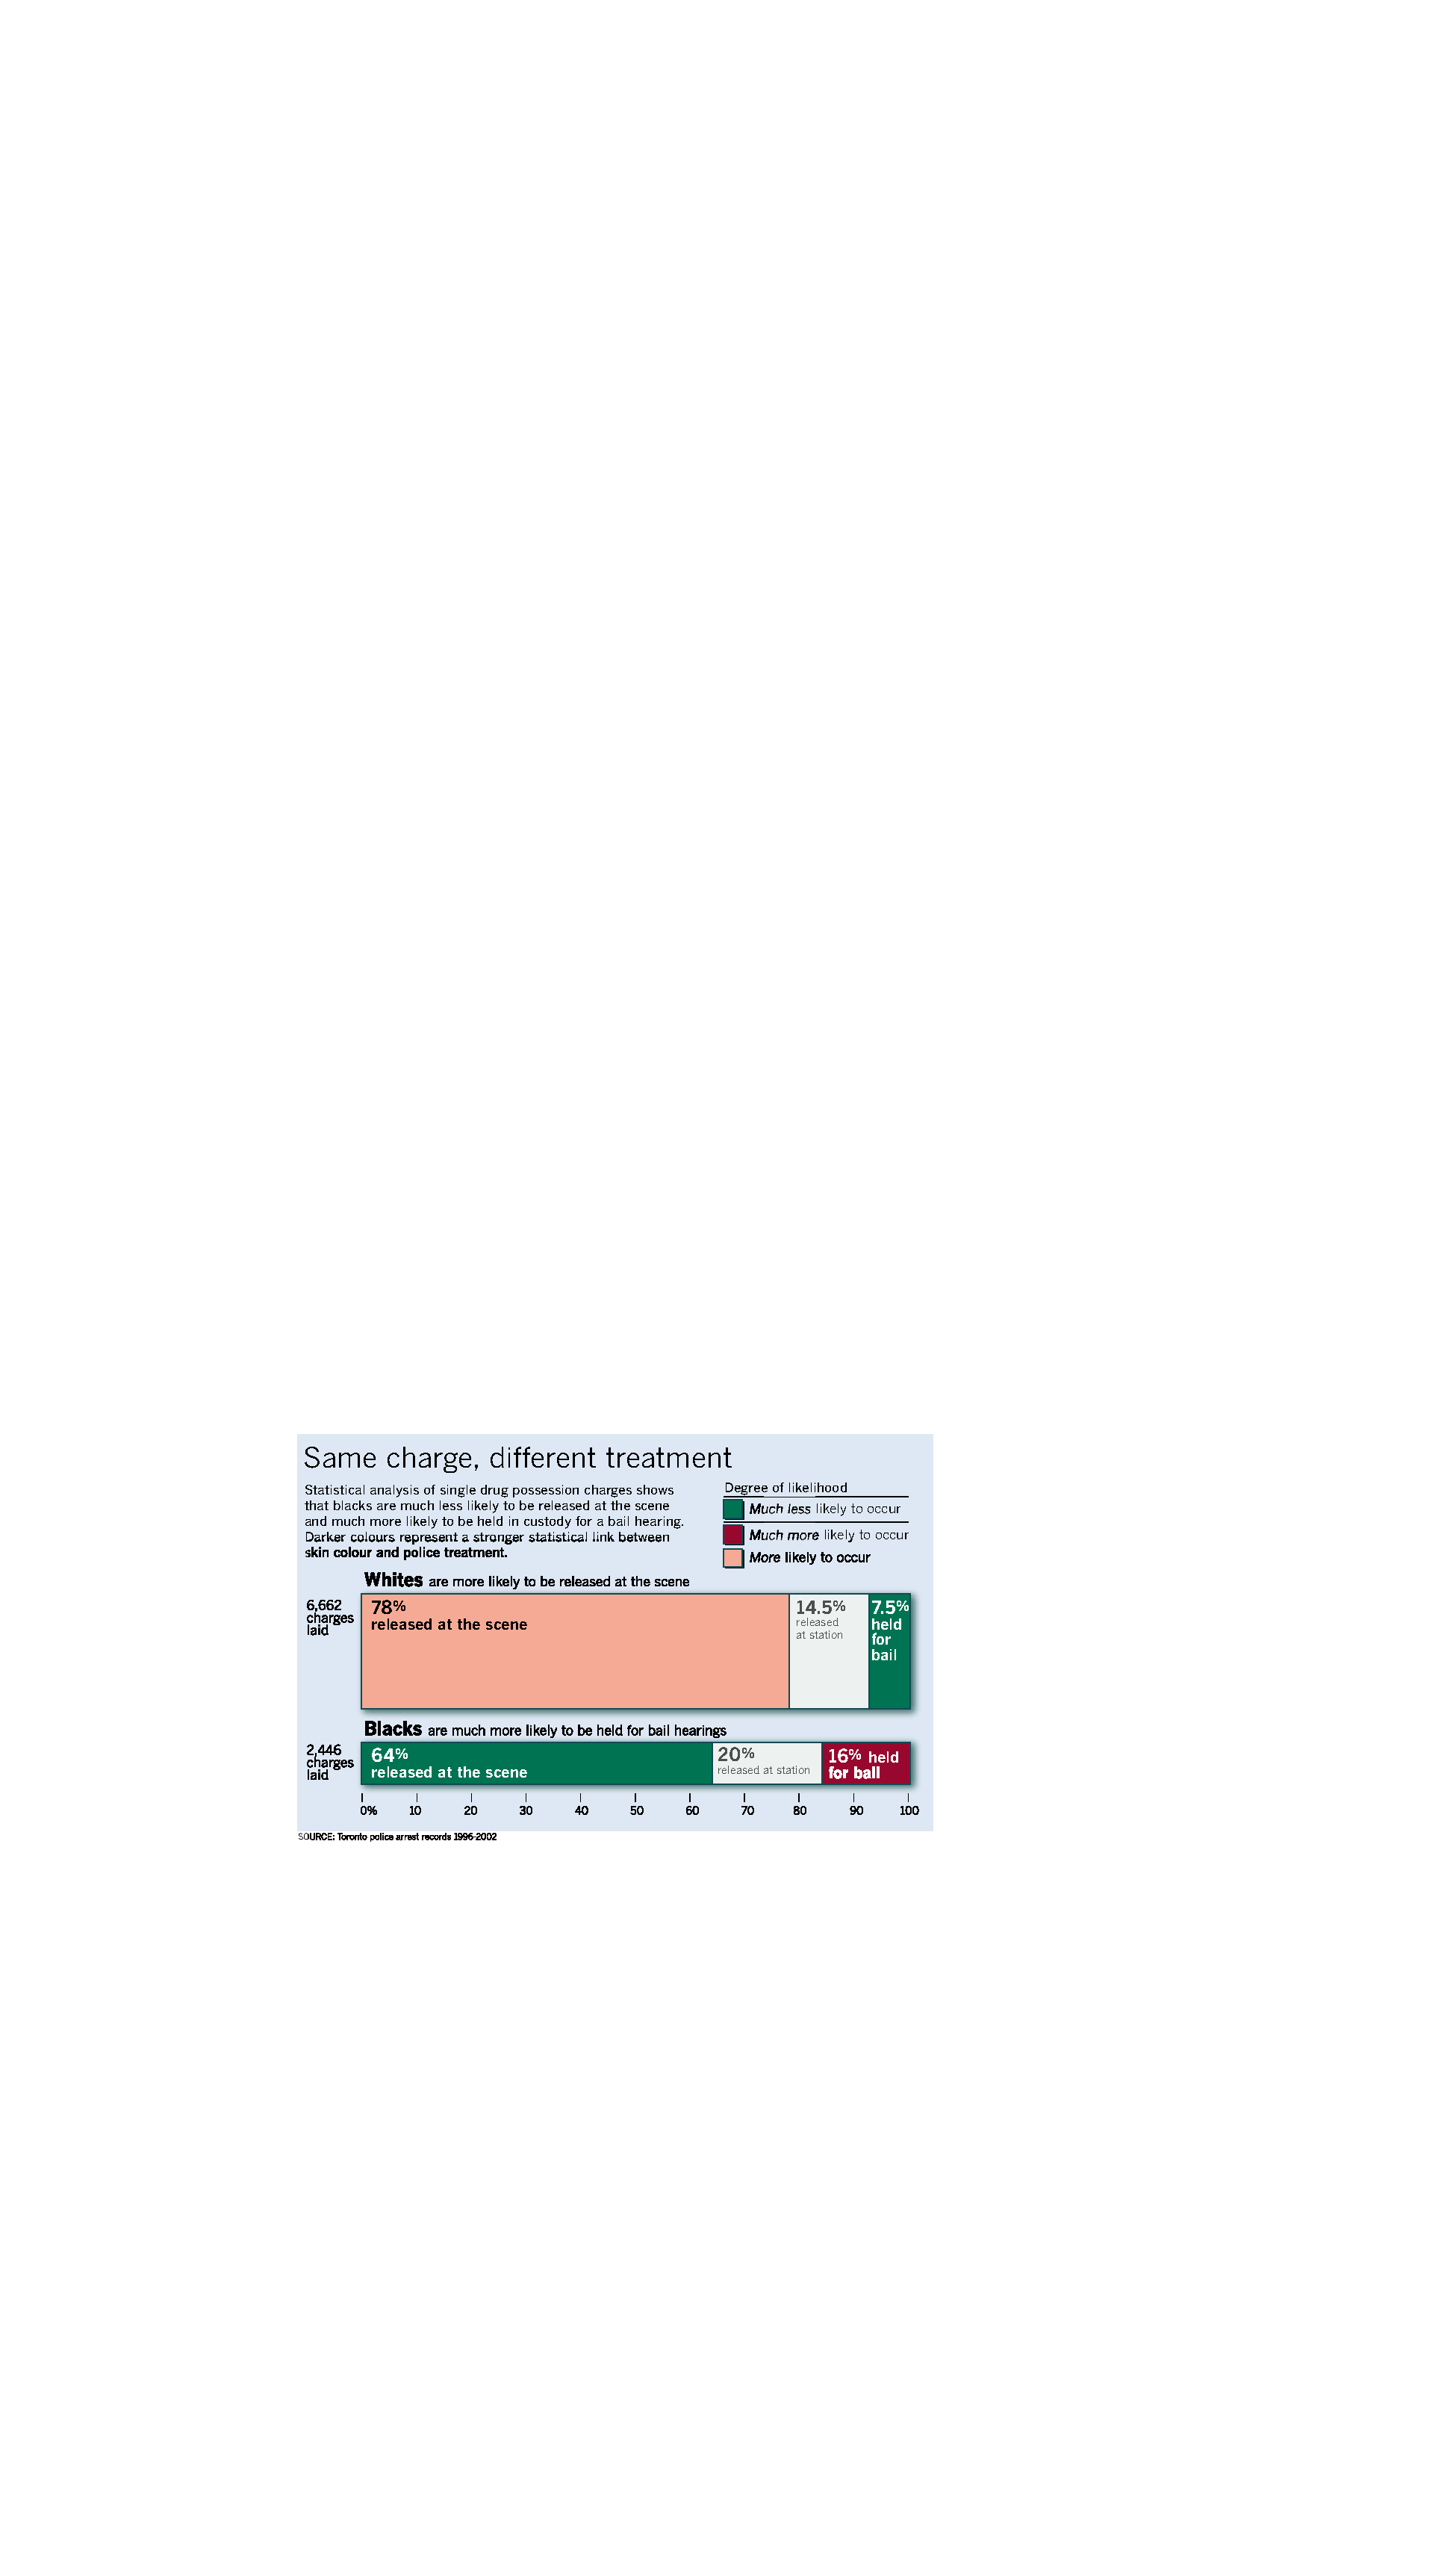
\includegraphics[width=.9\textwidth]{ch01/fig/TorontoStar-graphic-2002-12-11}
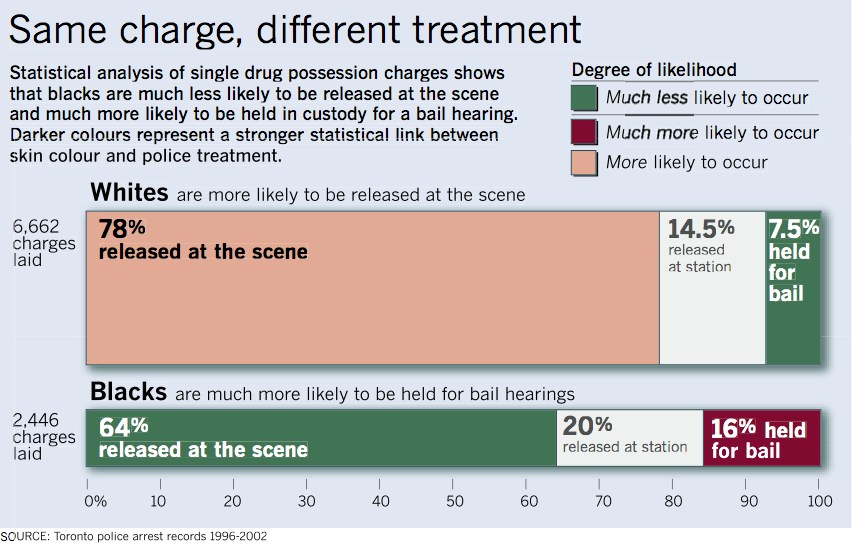
\includegraphics[width=.9\textwidth]{ch01/fig/TorStar/TorontoStar-graphic-2002-12-11-2}
\caption{Redesign of \figref{fig:arrests0-mosaic} as a presentation graphic. \emph{Source}: Graphics department, \emph{The Toronto Star}, December 11, 2002. Used by permission.}\label{fig:arrests0-star}
\end{figure}

Clear communication is not achieved without effort.  The revised graph required several iterations
and emails between the graphic designer and the statistical consultant (the first author of this book)
in the few hours available before the newspaper went to press.
The main question was, ``what are we trying to show here?'' Starting with the original
\figref{fig:arrests0-mosaic} mosaic, we asked ``what can we remove?'' and ``what can we add?''
to make the message clearer.

\end{Example}

\TODO{Complete this section.  Show a collection of analysis and presentation graphs for categorical data. It is probably better to wait until more chapters are written to provide examples here.}

\subsection{Categorical data require different graphical methods}\label{sec:intro-catdata}

We mentioned earlier, and will see in greater detail
in \chref{ch:logistic} and \chref{ch:loglin}
that statistical models for discrete
response data and for frequency
data are close analogs of the linear regression and ANOVA models
used for quantitative data.
These analogies suggest that the graphical methods
commonly used for quantitative data may be adapted directly to
categorical data.

Happily, it turns out that many of the analysis graphs and diagnostic
displays (e.g., effect plots,
influence plots, added variable and partial residual
plots, etc.)
that have become common adjuncts in the analysis of
quantitative data have been extended to generalized linear models
including logistic regression (\secref{sec:logist-infl})
and \loglin\ models (\secref{sec:glm-diag})
%\TODO{Add forward references to these sections.}

Unhappily, the familiar techniques for displaying raw data are
often disappointing when applied to categorical data.
The simple \scat, for example, widely used to show
the relation between
quantitative response and predictors, when applied to discrete
variables, gives a display of the category combinations,
with all identical values overplotted, and no representation of
their frequency.

Instead, frequencies of categorical variables are often best
represented graphically using \emph{areas} rather than as
position along a scale. \citet{Friendly:95} describes
conceptual and statistical models that give a rationale
for this graphic representation.
\figref{fig:arrests0-star} does this in the form of a
modified bar chart (mosaic plot), where the widths of the horizontal
bars show the proportions of whites and blacks in the data, and
the divisions of each group give the percents of each release type.
Consequently, the areas of each bar are proportional to the
frequency in the cells of this $2 \times 3$ table.

\begin{figure}
  \centering
  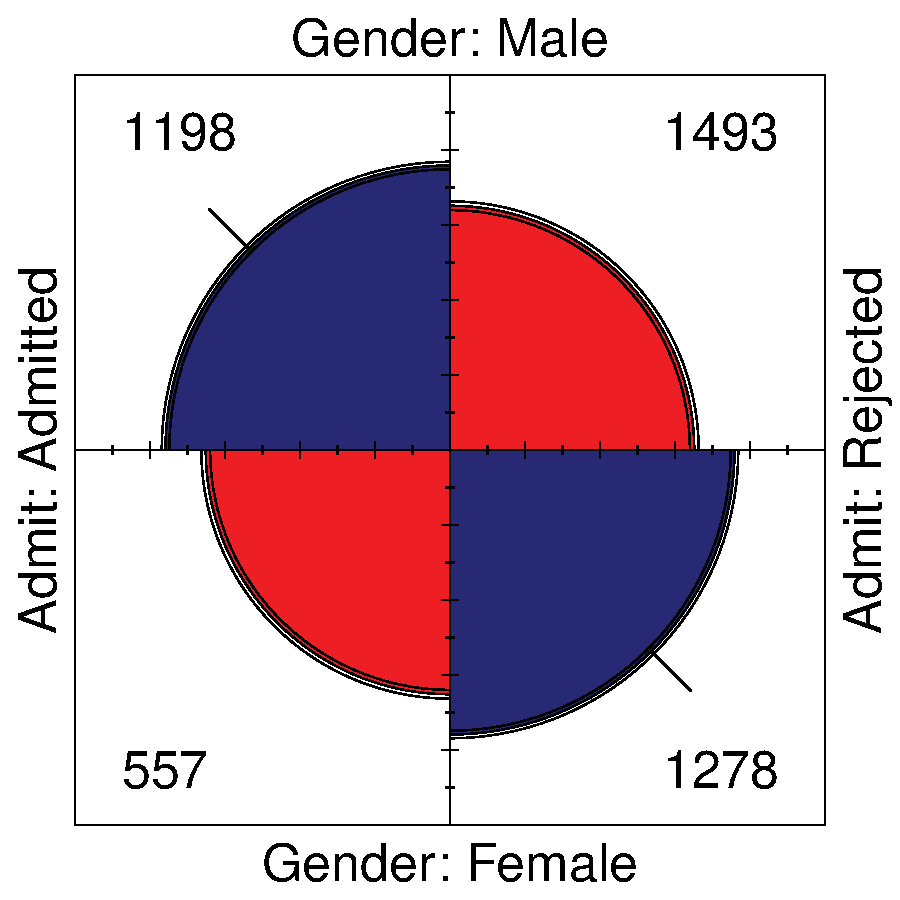
\includegraphics[width=0.49\textwidth]{ch01/fig/berk-fourfold3}
  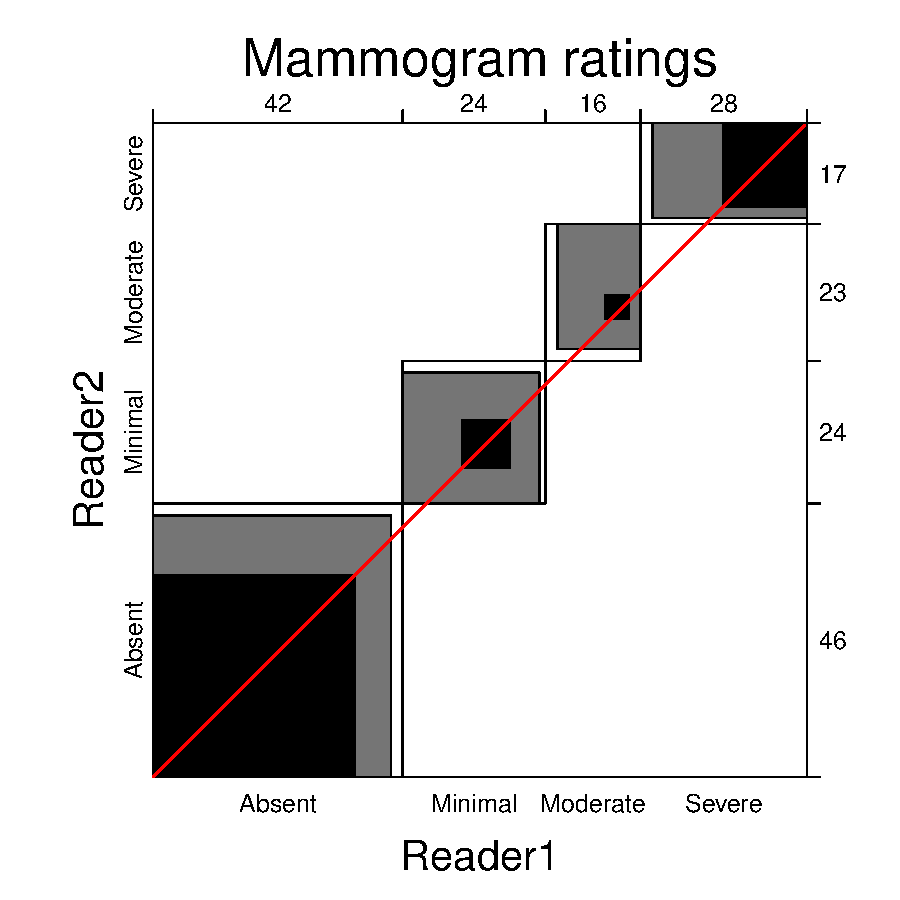
\includegraphics[width=0.49\textwidth]{ch01/fig/mammograms1}
  \caption{Frequencies of categorical variables shown as areas. Left: fourfold display of the relation between gender and admission in the Berkeley data; right: agreement plot for two raters assessing mammograms. }
  \label{fig:area-diagrams}
\end{figure}

As we describe later in this book, using the visual  attribute
\precept{area $\sim$ frequency}
also allows creating novel graphical displays of frequency data
for special circumstances.

\figref{fig:area-diagrams} shows two examples.
The left panel gives a \term{fourfold display} of the frequencies
of admission and gender in the Berkeley data shown in
\tabref{tab:berk220}.
What should be seen at a glance is that males are more often admitted
and females more often rejected (shaded blue); see \secref{sec:twoway-fourfold}
for details.

The right panel shows another specialized display, an \term{agreement chart}
designed to show the strength of agreement in a square table for two raters
(see \secref{sec:twoway-Bangdiwala}).  The example here (\exref{ex:mammograms})
concerns agreement of ratings of breast cancer from mammograms by two raters.
The dark squares along the diagonal show exact agreement; the lighter diagonal
rectangles allow 1-off agreement, and both are shown in relation to chance
agreement (diagonal enclosing rectangles).  What should be seen at a glance
is that exact agreement is moderately strong and extremely strong if you allow
the raters to differ by one rating category.


%\TODO{Complete this section.}

\subsection{Effect ordering and rendering for data display}\label{sec:effect-order}

In plots of quantitative variables, standard methods
(histograms, scatterplots) automatically position values along
ordered scales, facilitating comparison (``which is less/more?'')
and detection of patterns, trends and anomalies.
However, by its nature, categorical data involves discrete variables such as
education level, hair color, geographic region (state or province)
or preference for a political party.
With alphabetic labels for ordered
categories (e.g., education: Low, Medium, High), it is unfortunately all to
easy to end up with a nonsensical display with the categories
ordered High, Low, Medium.  Geographic regions (U.S. states) are often
ordered alphabetically by default as are the names of political parties
and other categorical variables.  This may be useful for lookup, but
for the purposes of comparison
and detection, this is almost always a bad idea.

Instead, \citet{FriendlyKwan:02:effect}, proposed the principle of
\term{effect-order sorting} for visual displays (tables as well as graphs):
% \begin{quote}
% \textbf{sort the data by the effects to be seen to facilitate comparison}
% \end{quote}
\precept{sort the data by the effects to be seen to facilitate comparison}
For quantitative data, this is often achieved by sorting the
data according to means or medians of row and column factors,
called \term{main-effect ordering}.
For categorical data, graphs and tables are often most effective
when the categories are arranged in an order reflecting their
association, called \term{association ordering}.

Another important principle concerns the
\term{rendering} of visual attributes of
elements in graphical displays
\citep{Friendly:02:corrgram}.  For example, categorical variables in plots (and tables)
can be distinguished by any one or more of color, size, shape, or font.
The examples below show the use of color to illustrate the precept:
% \begin{quote}
% \textbf{render the data by the effects to be seen to facilitate detection}
% \end{quote}
\precept{render the data by the effects to be seen to facilitate detection}

\begin{Example}[glass]{British social mobility}
\citet[p. 100]{Bishop-etal:75} analyzed data on the occupations of
3500 British fathers and their sons from a study by \citet{Glass:54},
with five occupational categories:
Professional, Managerial, Supervisory, Skilled manual and Unskilled manual.

One would expect, of course, a strong association between a son's
occupation and that of his father--- the apple doesn't
fall very far from the tree.
Mosaic plots (detailed in \chref{ch:mosaic})
provide a natural way to show such relationships.
\figref{fig:glass-mosaic} shows two such plots.
The left panel shows the result obtained when the table variables
\code{father} and \code{son} are read as factors, and therefore
ordered alphabetically by default.
It is difficult to see any overall pattern, except for the
large values in the diagonal cells (shaded blue) corresponding to equal
occupational status.

\begin{figure}
  \centering
  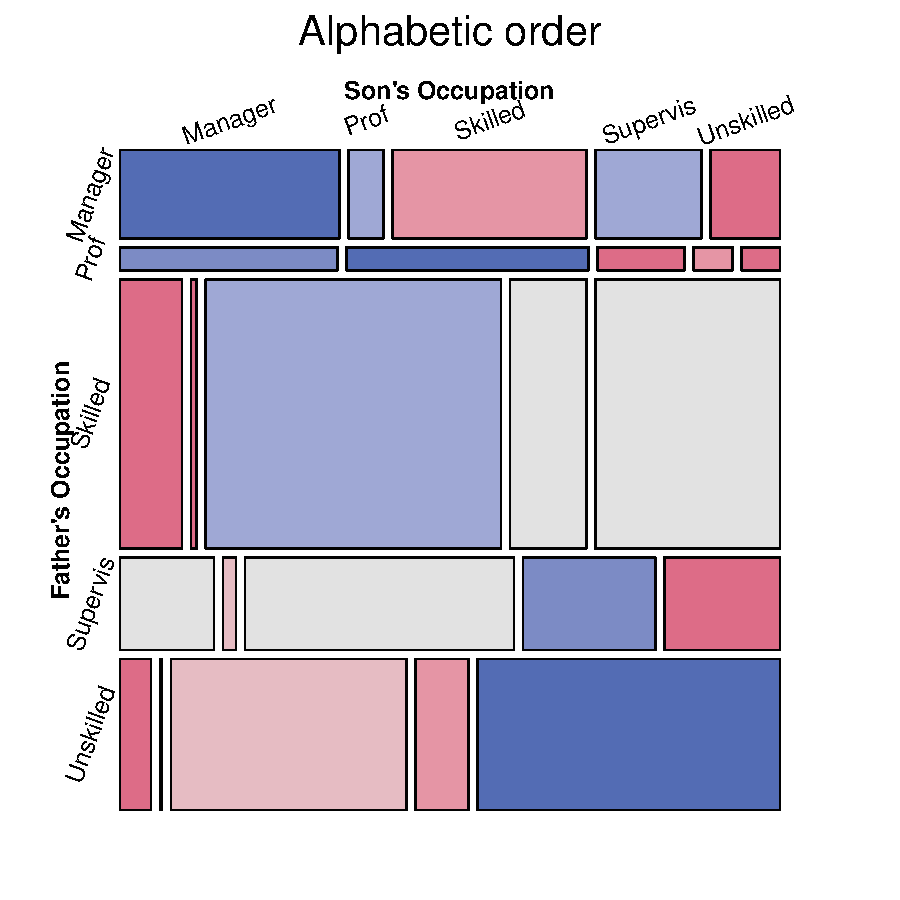
\includegraphics[width=0.49\textwidth]{ch01/fig/glass-mosaic1}
  \hfill
  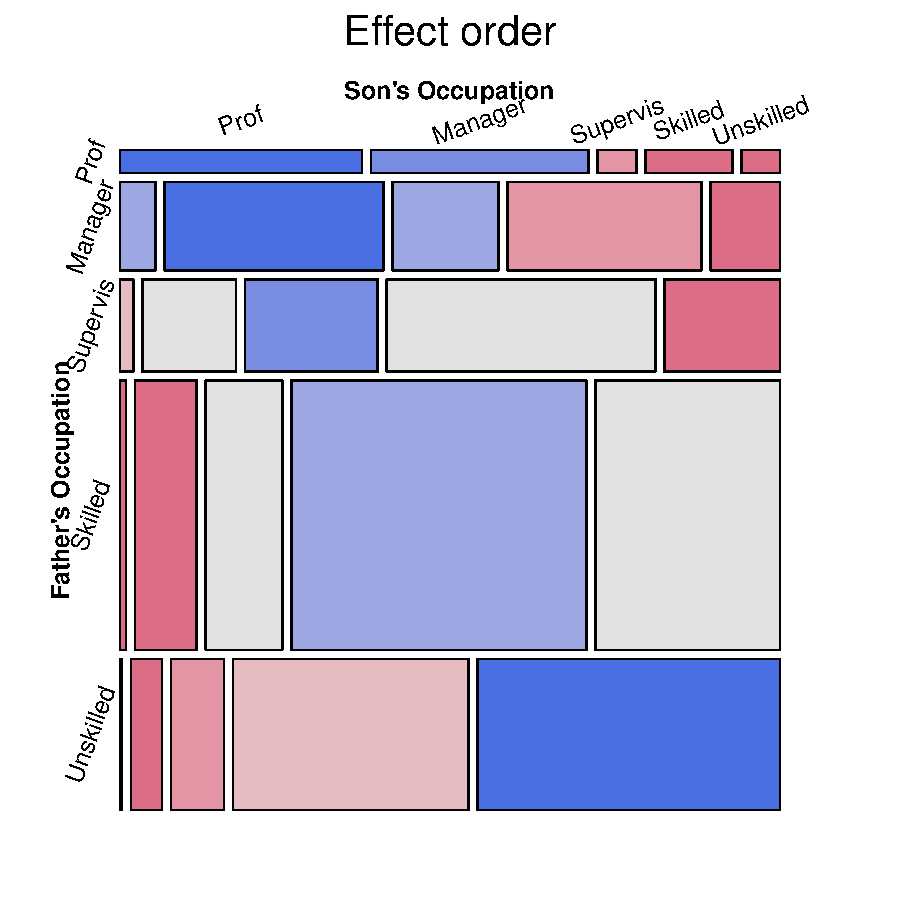
\includegraphics[width=0.49\textwidth]{ch01/fig/glass-mosaic2}
  \caption{Mosaic plots for Glass' mobility table of occupational status.
  In these displays the area of each tile is proportional to frequency
  and shading color shows the departure from independence, using
  blue for positive, red for negative association.
  Left: default alphabetic ordering of categories; right: occupational categories
  ordered by status.}
  \label{fig:glass-mosaic}
\end{figure}
In the right panel, the categories have been arranged in
decreasing order of occupational status to show the
association according to status.
Now you can see a global pattern of shading color, where the
tiles become increasingly red as one moves away from the main
diagonal, reflecting a greater difference between the occupation
of the father and son.
The interpretation here is that most sons remain in their
father's occupational class, but when they differ,
there is little mobility across large steps.

In this example, \code{father} and \code{son} are clearly ordinal
variables and should be treated as such in both graphs and statistical models.
Correspondence analysis (\chref{ch:corresp})
provides a natural way to depict association by assigning scores to
the categories to optimally represent their relationships.
\Loglin models provide special methods
for ordinal variables (\secref{sec:loglin-ordinal})
and square frequency tables (\secref{sec:loglin-square}).

\end{Example}

The ideas of effect ordering and rendering with
color shading to enhance perception can
also be used in tabular displays, as illustrated in the next example.

\begin{Example}[barley]{Barley data}
The classic \data{barley} dataset (in \pkg{lattice})
from \citet{Immer-etal:34}
gives a $10 \times 2 \times 6$ table of yields
of 10 varieties of barley in two years (1931, 1932)
planted at 6 different sites in Minnesota.
\citet{Cleveland:VisData} and many others have used this data to illustrate
graphical methods, and one
surprising finding not revealed in standard tabular displays
is that the data for one site (Morris) may have had
the values for 1931 and 1932 switched.%
\footnote{
This canonical story, like many others in statistics and graphics lore
turns out to be apocryphal on closer examination.
\cite{Wright:2013} recently took a closer look at the original data
and gives an expanded data set as \data{minnesota.barley.yield}
in the \Rpackage{agridat}.  With a wider range of years (1927--1936),
other local effects like weather had a greater impact than the
overall year effects seen in 1931--1932, and the results for the
Morris site no longer stand out as surprising.
}
This can easily be seen in a dotplot (not shown here)
of yield by variety, colored by year, and grouped by site.
The canonical graphical example can be produced
using \pkg{ggplot2} as follows:

\begin{knitrout}
\definecolor{shadecolor}{rgb}{1, 0.961, 0.933}\color{fgcolor}\begin{kframe}
\begin{alltt}
\hlkwd{data}\hlstd{(barley,} \hlkwc{package}\hlstd{=}\hlstr{"lattice"}\hlstd{)}
\hlkwd{library}\hlstd{(ggplot2)}
\hlkwd{ggplot}\hlstd{(}\hlkwc{data}\hlstd{=barley,} \hlkwd{aes}\hlstd{(}\hlkwc{x}\hlstd{=yield,} \hlkwc{y}\hlstd{=variety,} \hlkwc{color}\hlstd{=year))} \hlopt{+}
  \hlkwd{geom_point}\hlstd{()} \hlopt{+}
  \hlkwd{facet_wrap}\hlstd{(}\hlopt{~}\hlstd{site)}
\end{alltt}
\end{kframe}
\end{knitrout}

To focus attention on this suspicious effect in a tabular display,
you can calculate the \emph{yield difference}
$\Delta y_{ij} = y_{ij,1931} - y_{ij,1932}$ and arrange these
in a $10 \times 6$ table as shown below. \TODO{This is not correct. FIXME}

\begin{knitrout}
\definecolor{shadecolor}{rgb}{1, 0.961, 0.933}\color{fgcolor}\begin{kframe}
\begin{alltt}
\hlstd{yield} \hlkwb{<-} \hlkwd{array}\hlstd{(barley}\hlopt{$}\hlstd{yield,} \hlkwd{c}\hlstd{(}\hlnum{6}\hlstd{,} \hlnum{10}\hlstd{,} \hlnum{2}\hlstd{))}
\hlkwd{dimnames}\hlstd{(yield)} \hlkwb{<-} \hlkwd{list}\hlstd{(}
  \hlkwc{site} \hlstd{=} \hlkwd{levels}\hlstd{(barley}\hlopt{$}\hlstd{site),}
  \hlkwc{variety} \hlstd{=} \hlkwd{levels}\hlstd{(barley}\hlopt{$}\hlstd{variety),}
  \hlkwc{year} \hlstd{=} \hlkwd{levels}\hlstd{(barley}\hlopt{$}\hlstd{year))}
\hlstd{diff} \hlkwb{<-} \hlkwd{t}\hlstd{(yield[,,}\hlnum{2}\hlstd{]} \hlopt{-} \hlstd{yield[,,}\hlnum{1}\hlstd{])}
\end{alltt}
\end{kframe}
\end{knitrout}

\definecolor{blueA}{rgb}{0.85,0.85,1}
\definecolor{blueB}{rgb}{0.7 ,0.7 ,1}
\definecolor{redA}{rgb}{1,0.85,0.85} 
\definecolor{redB}{rgb}{1,0.7 ,0.7 } 
%%
%% Table barley2c written by md2tex 17AUG00 17:52
%%
\begin{table}[htb]
 \caption{Barley data, yield differences, 1931-1932, sorted by mean difference, and shaded by value}
 \label{tab:barley2c}
 \begin{center}
  \begin{tabular}{|l|rrrrrr|r|}
   \hline
 & \multicolumn{6}{c|}{\bfseries\large Site   } & \rule{0in}{2.5ex}\\
{\bfseries\large Variety} &  Morris &  Duluth & \brk{University\\Farm} & \brk{Grand\\Rapids} &  Waseca &  Crookston& {\bfseries\large\itshape Mean} \\
   \hline
\multirow{1}*{No. 475} & \cell{redB}{-22} &               6 &              -5 &               4 &               6 & \cell{blueB}{12} &             0.1 \\
\multirow{1}*{Wisconsin No. 38} & \cell{redB}{-18} &               2 &               1 & \cell{blueB}{14} &               1 & \cell{blueB}{14} &             2.4 \\
\multirow{1}*{Velvet} & \cell{redB}{-13} &               4 & \cell{blueB}{13} & \cell{redA}{-9} & \cell{blueB}{13} & \cell{blueA}{9} &             2.9 \\
\multirow{1}*{Peatland} & \cell{redB}{-13} &               1 &               5 & \cell{blueA}{8} & \cell{blueB}{13} & \cell{blueB}{16} &             4.8 \\
\multirow{1}*{Manchuria} & \cell{redA}{-7} & \cell{blueA}{6} &               0 & \cell{blueB}{11} & \cell{blueB}{15} & \cell{blueA}{7} &             5.5 \\
\multirow{1}*{Trebi} &              -3 &               3 & \cell{blueA}{7} & \cell{blueA}{9} & \cell{blueB}{15} &               5 &             6.1 \\
\multirow{1}*{Svansota} & \cell{redA}{-9} &               3 & \cell{blueA}{8} & \cell{blueB}{13} & \cell{blueA}{9} & \cell{blueB}{20} &             7.3 \\
\multirow{1}*{No. 462} & \cell{redB}{-17} &               6 & \cell{blueB}{11} &               5 & \cell{blueB}{21} & \cell{blueB}{18} &             7.4 \\
\multirow{1}*{Glabron} & \cell{redA}{-6} &               4 &               6 & \cell{blueB}{15} & \cell{blueB}{17} & \cell{blueB}{12} &             8.0 \\
\multirow{1}*{No. 457} & \cell{redB}{-15} & \cell{blueB}{11} & \cell{blueB}{17} & \cell{blueB}{13} & \cell{blueB}{16} & \cell{blueB}{11} &             8.8 \\
   \hline
\rule{0in}{2.5ex}{\bfseries\large\itshape Mean} &          -12.2 &             4.6 &             6.3 &             8.2 &            12.5 &            12.5 &             5.3 \\
   \hline
  \end{tabular}
 \end{center}
\end{table}


\tabref{tab:barley2c} shows these values in a table with the rows and columns
sorted by their means (main-effect ordering).  In addition, the table cells
have been colored according to the sign and magnitude of the year difference.
The shading scheme uses blue for large positive values and red for large
positive values, with a white background for intermediate values.
The shading intensity values were determined as
$| \Delta y_{ij} |> \{2, 3\} \times \widehat{\sigma} (\Delta y_{ij} )$.

Effect ordering and color rendering
have the result of revealing a new effect, shown as a regular progression
in the body of the table.
The negative values for Morris now immediately stand out.  In addition,
the largely positive other values show a lower-triangular pattern,
with the size of the yield difference increasing with both row and column means.
Against this background, one other cell, for Velvet grown at Grand Rapids stands out
with an anomalous negative value.

Although the use of color for graphs is now more common in some journals,
color and other rendering details in tables are still difficult.
The published version of \tabref{tab:barley2c} \citep[Table 3]{FriendlyKwan:02:effect}
was forced to use only font shape (normal, italics) to distinguish positive and
negative values.

\end{Example}

Finally, effect ordering is also usefully applied to the variables in multivariate data
sets, which by default, are often ordered in data displays according to their position
in a data frame or alphabetically.

\begin{Example}{Iris data}
The classic \data{iris} data set \citep{Anderson:35,Fisher:36}
gives the measurements in centimeters of the variables sepal length and width and petal length and width, respectively, for 50 flowers from each of 3 species of iris, \emph{Iris setosa}, \emph{versicolor}, and \emph{virginica}.
Such multivariate data are often displayed in \term{parallel coordinate plot}s, using a separate vertical axis for
each variable, scaled from its minimum to maximum.

The default plot, with variables shown in their data frame order is shown in the left panel of \figref{fig:iris-parallel},
and gives rise to the epithet \emph{spaghetti plot} for such displays because of the large number of line crossings.
This feature arises because one variable, sepal width, has negative relations in the species means with the other
variables. Simple rearrangement of the variables to put sepal width last (or first)
makes the relations among the species and the variables more apparent, as shown in the right panel of \figref{fig:iris-parallel}.  This plot has also been enhanced by using \term{alpha-blending} (partial transparency) of thicker
lines, so that the density of lines is more apparent.

\begin{knitrout}
\definecolor{shadecolor}{rgb}{1, 0.961, 0.933}\color{fgcolor}\begin{figure}[!htbp]


\centerline{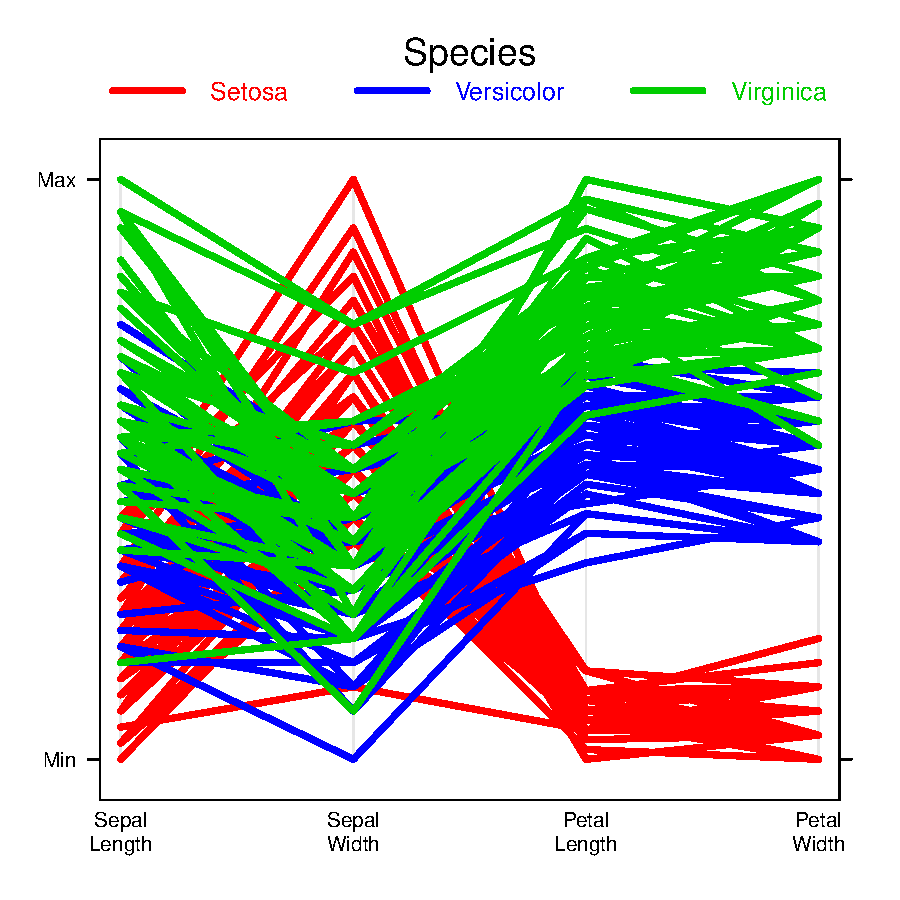
\includegraphics[width=.49\textwidth]{ch01/fig/iris-parallel-1} 
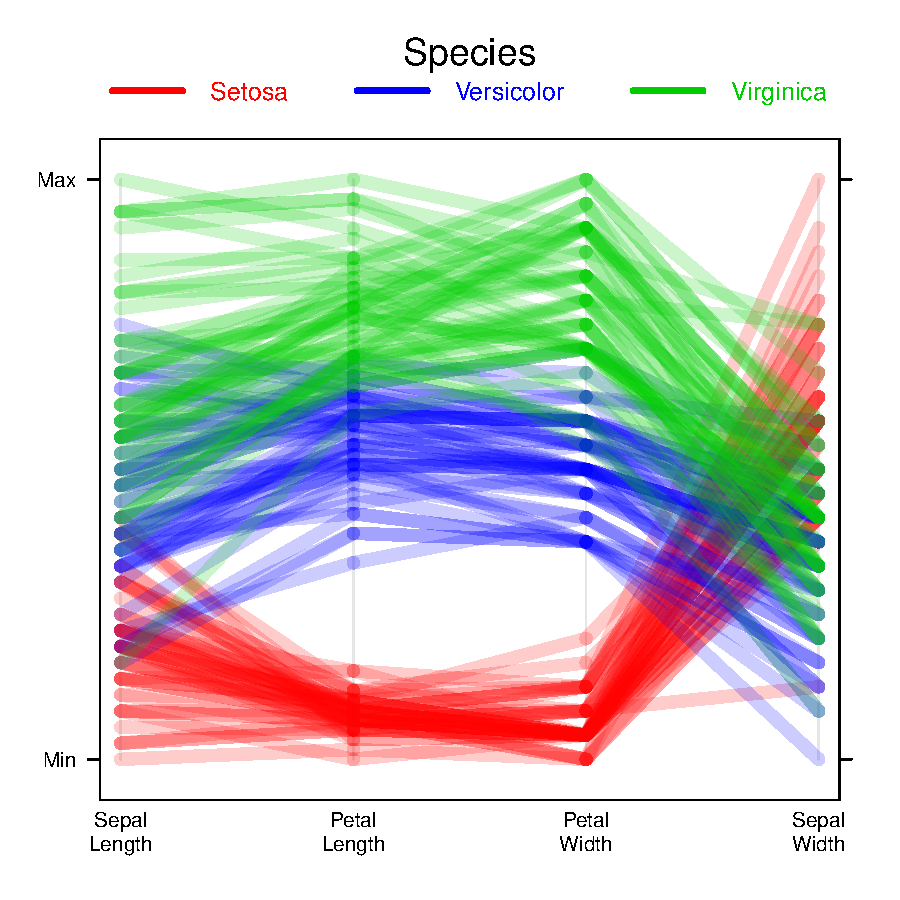
\includegraphics[width=.49\textwidth]{ch01/fig/iris-parallel-2} }

\caption[Parallel coordinates plots of the Iris data]{Parallel coordinates plots of the Iris data. Left: Default variable order; right: Variables ordered to make the pattern of correlations more coherent.\label{fig:iris-parallel}}
\end{figure}


\end{knitrout}
Parallel coordinate plots for categorical data are discussed in \secref{sec:parallel}.
A general method for reordering variables in multivariate data visualizations based on
cluster analysis was proposed by \citet{Hurley:2004}.


\end{Example}

\subsection{Interactive and dynamic graphics}\label{sec:intro-interactive}

%\subsection{Interactive and dynamic graphics}\label{sec:intro-interactive}

Graphics displayed in print form, such as this book, are necessarily static
and fixed at the time they are designed and rendered as an image.
Yet, recent developments in software, web technology and media
alternative to print have created the possibility to extend graphics
in far more useful and interesting ways, for both presentation
and analysis purposes.

Interactive graphics
\ix{interactive graphics}
\ix{graphics!interactive}
allow the viewer to directly manipulate the
statistical and visual components of graphical display.  These
range from
\begin{itemize*}
\item graphical controls (sliders, selection boxes and other widgets)
to control details of an analysis (e.g., a smoothing parameter) or graph
(colors and other graphic details), to
\item higher-level interaction including zooming in or out,
drilling down to a data subset,
linking multiple displays, selecting terms in a model and so forth.
\end{itemize*}
The important effect is that the analysis and/or display is immediately
re-computed and updated visually.

In addition, \term{dynamic graphics} use animation to show a series of
views, as frames in a movie.  Adding time as an additional
dimension allows far more possibilities, for example
showing a rotating view of a 3D graph or showing smooth transitions
or interpolations from one view to another.

There are now many packages in \R providing interactive and dynamic plots
(e.g., \pkg{rggobi}, \pkg{iplots})
as well as capabilities to incorporate these into interactive documents,
presentations and web pages (e.g., \pkg{rCharts}, \pkg{googleVis}).
The \Rpackage{animate} facilitates creating animated graphics  and movies in a
variety of formats.
The RStudio editor and development environment%
\footnote{\url{http://www.rstudio.com}}
provides its own
\Rpackage{manipulate}, as well as the \pkg{shiny} framework for
developing interactive \R web applications.

\begin{Example}[512paths]{512 paths to the White House}
Shortly before the 2012 U.S. presidential election (November 2, 2012)
the \emph{New York Times} published an interactive graphic%
\footnote{\url{http://www.nytimes.com/interactive/2012/11/02/us/politics/paths-to-the-white-house.html}},
designed by Mike Bostock And Shan Carter.%
\footnote{
see: \url{https://source.opennews.org/en-US/articles/nyts-512-paths-white-house/}
for a description of their design process.}
showing
the effect that a win for Barack Obama or Mitt Romney in the
nine most highly contested states would have on the chances
that either candidate would win the presidency.

\begin{figure}
\centering
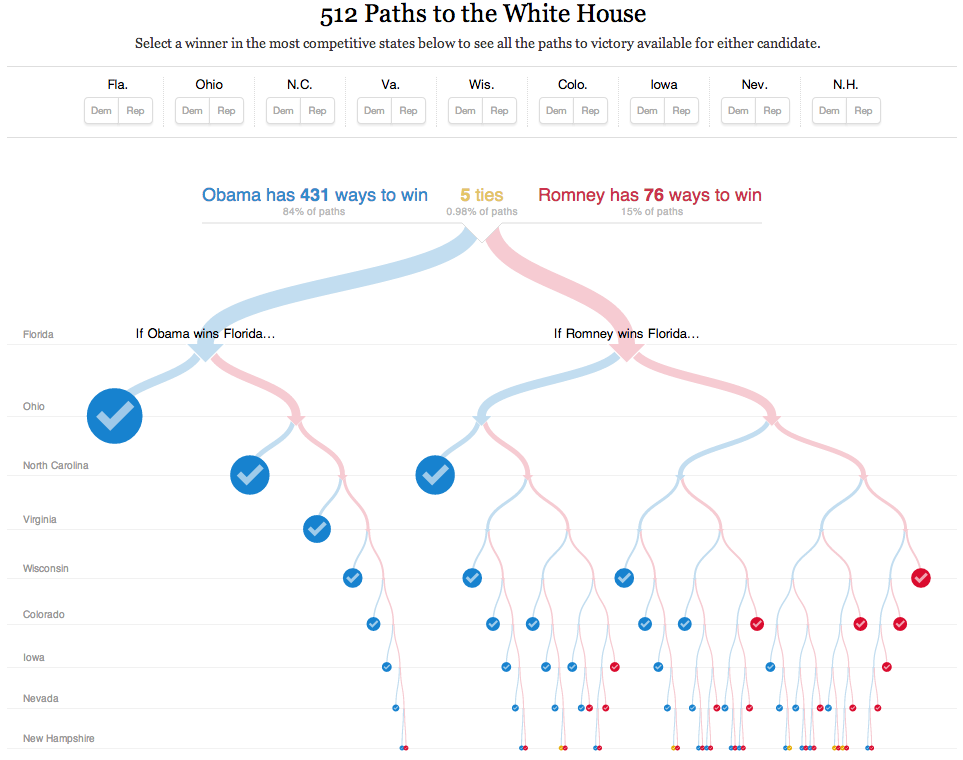
\includegraphics[width=0.7\textwidth]{ch01/fig/nyt_512paths.png}
\caption{512 paths to the White House.  This interactive graphic allows the viewer to
select a winner in any one or more of the nine most highly contested U.S. states
and highlights the number of paths leading to a win by Obama or Romney, sorted and
weighted
by the number of Electoral College votes.}
\label{fig:nyt_512paths}
\end{figure}

With these nine states most in play there are $2^9 = 512$ possible outcomes
but with different number of votes in the Electorial College.
In \figref{fig:nyt_512paths}, a win for Obama in Florida and Virginia was
selected, with wins for Romney in Ohio and North Carolina.
Most other selections also lead to a win by Obama, but those with
the most votes are made most visible at the top.
An \R version of this chart was created using the \Rpackage{rCharts}.%
\footnote{
\url{http://timelyportfolio.github.io/rCharts_512paths/}
}
The design of this graphic as a \term{binary tree} was chosen here, but
another possibility would be a \term{treemap} graphic
\citep{Shneiderman:92} or a mosaic plot.


\end{Example}




\section{Visualization = Graphing + Fitting + Graphing $\dots$}\label{sec:vis}
\epigraph{Look here, upon this picture, and on this.}{Shakespeare, Hamlet}

Statistical summaries, hypothesis tests, and the numerical parameters
derived in fitted models are designed to capture a particular feature of the
data.  A quick analysis of the data from \tabref{tab:berk220}, for example,
shows that
1198/2691 = 44.5\% of male applicants were admitted, compared to
557/1835 =30.4\% of female applicants.

Statistical tests
give a Pearson $\chi^2$ of 92.2
with 1 degree of freedom
for association between admission and gender ($p < 0.001$), and
various measures for the strength of association.
% <<UCBstats>>=
% UCB <- margin.table(UCBAdmissions, 1:2)
% assocstats(UCB)
% oddsratio(UCB, log=FALSE)
% @
%
Expressed in terms of the \term{odds ratio}, males were apparently
1.84 times as likely
to be admitted as females, with 99\% confidence bounds
1.56--2.17.
Each of these numbers expresses some part of the relationship between
gender and admission in the Berkeley data.
Numerical summaries such as these are each
designed to compress the information in the data, focusing on some particular
feature.
\TODO{Use this for a lab exercise in Ch 2.}

In contrast, the visualization approach to data analysis is designed
to
\begin{seriate}
\item expose information and structure in the data,
\item supplement the information available from numerical summaries, and
\item suggest more adequate models.
\end{seriate}
In general, the visualization approach seeks to serve the needs of
both summarization and exposure.

This approach recognizes that both data analysis and graphing are
\emph{iterative} processes.
You should not expect that any one model captures all features of the
data, any more than we should expect that a single graph shows all that
may be seen.  In most cases, your initial steps should include some
graphical display guided by understanding of the subject matter
of the data.
What you learn from a graph may then help suggest features of the data
to be incorporated into a fitted model.
Your desire to ensure that the fitted model is an adequate summary
may then lead to additional graphs.

The precept here is that
\precept{Visualization = Graphing + Fitting + Graphing $\dots$}
where the ellipsis indicates the often iterative nature of this process.
Even for descriptive purposes, an initial fit of salient features can be
removed from the data, giving residuals (departures from a model).
Displaying the residuals may then suggest additional features to account for.

Simple examples of this idea include detrending time series graphs to remove
overall and seasonal effects and plots of residuals from main-effect models
for ANOVA designs.  For categorical data, mosaic plots (\chref{ch:mosaic})
display the unaccounted-for association between variables by shading,
as in \figref{fig:glass-mosaic}.  Additional models and plots
considered in \secref{sec:loglin-square} can reveal additional structure
in square tables beyond the obvious effect that sons tend most often to
follow in their fathers' footsteps.

\begin{Example}[donner0a]{Donner party}
The graphs in \figref{fig:donner0} and \figref{fig:donner0-other}
suggest three different initial descriptions for survival in the
Donner party.  Yet they ignore all other influences, of which
gender and family structure might also be important.
A more complete understanding of this data can be achieved
by taking these effects into account, both in fitted models
and graphs.  See \exref{ex:donner1} for a continuation of this story.
\end{Example}

\begin{Example}[nasa]{Space shuttle disaster}

The space shuttle \emph{Challenger} mentioned in \exref{ex:nasa0}
exploded 73 seconds after take-off on
January 28, 1986.
Subsequent investigation presented to the presidential commission
headed by William Rogers
determined that the cause was failure of the O-ring
seals used to isolate the fuel supply from burning gases.
The story behind the \emph{Challenger} disaster is perhaps the most poignant
missed opportunity in the history of statistical graphics.
See \citet{Tufte:97} for a complete exposition.
It may be heartbreaking to find out that some important information
was there, but the graph maker missed it.

\begin{figure}[htb]
  \centering
  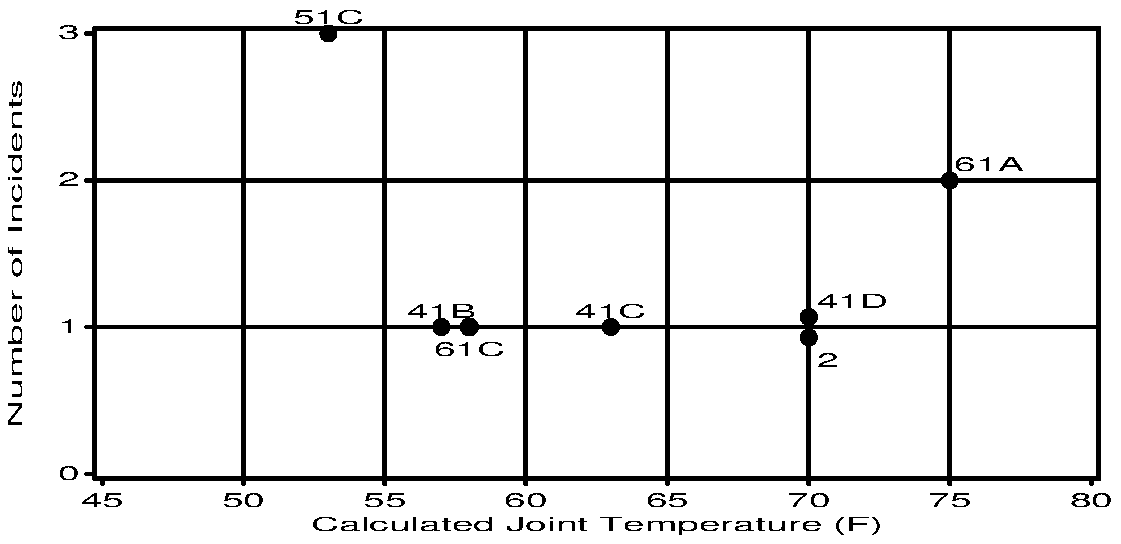
\includegraphics[width=\textwidth,clip]{ch01/fig/nasa0}
  \caption{NASA Space Shuttle pre-launch graph prepared by the engineers at Morton Thiokol}\label{fig:nasa0}
\end{figure}

Engineers from Morton Thiokol, manufacturers of the rocket motors,
had been worried about the effects of unseasonably cold weather
on the O-ring seals and recommended aborting the flight.
NASA staff analysed the data, tables and charts submitted by
the engineers and concluded that there was insufficient evidence
to cancel the flight.

The data relating O-ring failures to temperature were depicted as in
\figref{fig:nasa0}, our candidate for the most misleading graph in history.
There had been 23 previous launches of these rockets giving data on
the number of O-rings (out of 6) that were seen to have suffered
some damage or failure. However, the engineers omitted the observations
where no O-rings failed or showed signs of damage, believing that they were uninformative.

Examination of this graph seemed to indicate that there was no relation
between ambient temperature and failure.
Thus, the decision to launch
the \emph{Challenger} was made, in spite of the initial concerns
of the Morton Thiokol engineers.
Unfortunately, those observations had occurred when the launch temperature
was relatively warm (\degree{65-80}F.) and were indeed informative.
The coldest temperature at any previous launch was \degree{53};  when \emph{Challenger} was launched on January 28,
the temperature was a frigid \degree{31}.

These data have been analyzed extensively
\citep{Dalal-etal:89,Lavine:91}.
\citet{Tufte:97} gives a thorough and convincing
visual analysis of the evidence available prior to the launch.
We consider statistical analysis of these data in \chref{ch:logistic},
\exref{ex:nasa-temp}.

But, what if the engineers had simply made a better graph?
At the very least, that would entail
\begin{seriate}
\item drawing a smoothed curve to fit the points (to show the trend)
\item removing the background grid lines (which obscure the data).
\end{seriate}
\figref{fig:nasa}
shows a revised version of the same graph, highlighting the
the non-zero observations and adding a simple quadratic
curve to allow for a possible non-linear relationship.
For comparison, the excluded zero observations are also
shown in grey.
This plot, even showing only the non-zero points
should have caused any engineer to conclude that
either:
\begin{seriate}
\item the data were wrong, or
\item there were excessive risks
associated with both high and low temperatures.
\end{seriate}
But it is well-known
that brittleness of the rubber used in the O-rings is inversely
proportional to Temperature$^3$, so prudent interest might have focussed
on the first possibility.

\begin{figure}[htb]
  \centering
  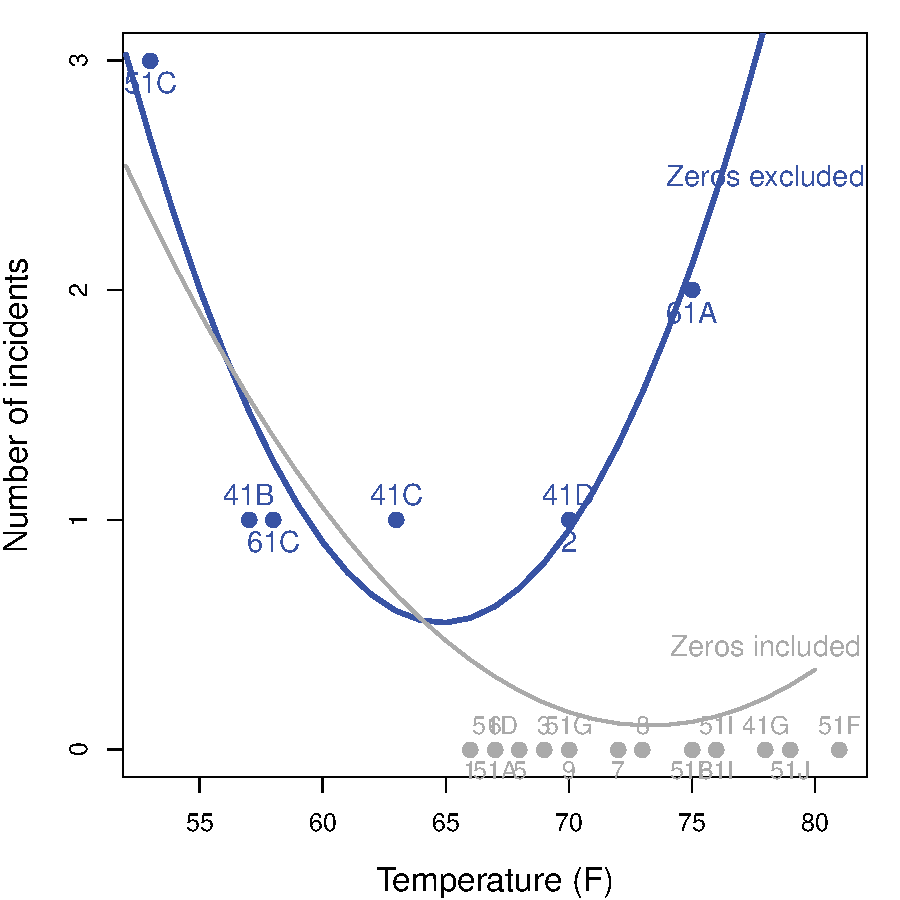
\includegraphics[width=.7\textwidth,clip]{ch01/fig/nasa}
  \caption{Re-drawn version of the NASA pre-launch graph, showing the locations of the excluded observations and with fitted quadratics for both sets of observations}\label{fig:nasa}
\end{figure}

%\TODO{Add coda: Feynman O-ring demonstration to the Rogers Commission}
A coda to this story shows the role of visual explanation in practice as well
\citep[p. 50--53]{Tufte:97}.
The Rogers Commission contracted the reknown theoretical physicist Richard Feynman
to contribute to their investigation.  He determined that the most probable
cause of the shuttle failure was the lack of resiliancy of the rubber O-rings
at low temperature. But how could he make this point convincingly?
At a televised public hearing, he took a piece of the O-ring material,
squeezed it in C-clamp and plunged it into a glass of ice water.
After a few minutes, he released the clamp, and the rubber did not spring
back to shape.  He mildly said,
``... there is no resilience in this particular material when it is at a
temperature of 32 degress. I believe this has some significance for our
problem'' \citep{Feynman:1988}.

\end{Example}

\subsection{The 80-20 rule}
The Italian economist Vilfredo Pareto observed in 1906 that 80\% of the land in Italy was
owned by 20\% of the population and this ratio also applied in other countries. 
It also applied to the yield of peas from peapods in his garden \citep{Pareto:1971}.
This idea became known as the
\term{Pareto principle} or the \term{80--20 rule}.
The particular 80/20 ratio is not as important as the more general idea of the
uneven distribution of results and causes in a variety of areas.

Common applications are the rules of thumb that: 
\begin{seriate}
  \item in business 80\% of sales come from 20\% of clients; 
  \item in criminology 80\% of crimes are said to be committed by 20\% of the population.
  \item In software development, it is said that 80\% of errors and 
  \item crashes can be eliminated by fixing the top 20\% most reported bugs
or that 80\% of errors reside in 20\% of the code.
\end{seriate}

The \term{Pareto chart} was designed to display the frequency distribution of
a variable with a histogram or bar chart together with a cumulative line graph
to highlight the most frequent category, and the \term{Pareto distribution}
gives a mathematical form to such distributions with a parameter $\alpha$
(the \emph{Pareto index})
reflecting the degree of inequality.

Applied to statistical graphics, the precept is that
\precept{20\% of your effort can generate
80\% of your desired result in producing a given plot.}
This is good news for exploratory
graphs you produce for yourself.  Very often, the default settings will give a reasonable
result, or you will see immediately something simple to add or change to make the plot
easier to understand.

The bad news is the corollary of this rule:
\precept{
80\% of your effort may be required to produce the remaining 20\% of a finished graph.
}
This is particularly important for presentation graphs, where several iterations
may be necessary to get it right (or right enough) for your communication purposes.
Some important details are:
\begin{description}

\item[graph title] A presentation graphic can be more effective when it announces
 the main point or conclusion in the graphic title, as in \figref{fig:arrests0-star}.

\item[axis and value labels] Axes should be labelled with meaningful variable descriptions
 (and perhaps the data units) rather than just plot defaults (e.g., ``Temperature (degrees F)''
 in \figref{fig:spaceshuttle0}, not \code{temp}).
 Axis values are often more of a challenge for categorical variables, where their text
 labels often overlap, requiring abbreviation, a smaller font or text rotation.

\item[grouping attributes] Meaningfully different subsets of the data should be
 rendered with distinct visual attributes such as color, shape, and line style,
 and sometimes with more than one.

 \item[legends and direct labels] Different data groups in a graphic display
 shown by color, shape, etc.  usually need at least a graphic legend defining
 the symbols and group labels. Sometimes you can do better by applying the
 labels directly to the graphical elements,%
 \footnote{
 For example, the \func{identify} function allows points in a plot to be labeled
 interactively with a mouse.  The \Rpackage{directlabels} provides a general
 method for a variety of plots.
 }
 as was done in \figref{fig:nasa}.

 \item[legibility] A common failure in presentation graphs in journals
 and lectures is the use of text fonts too small to be read easily.
 One rule of thumb is to hold the graph at arms length for a journal
 and put it on the floor for a lecture slide.  If you can't read the
 labels, the font is too small.

 \item [plot annotations] Beyond the basic graphic data display, additional
 annotations can add considerable information to interpret the context
 or uncertainty, as in the use of plot envelopes to show confidence bands
 or regions (see \figref{fig:donner0} and \figref{fig:donner0-other}).

 \item[aspect ratio] Line graphs (such as \figref{fig:arbuthnot1})
 are often easiest to understand when the ratio of
 height to width is such that line segments have an average slope
 near 1.0 \citep{Cleveland-etal:88:shape}.
 In \R, you can easily manipulate a graph window manually with a
 mouse to observe this effect and find an aspect ratio that looks
 right.

 Moreover, in graphs for biplots and \ca (\chref{ch:corresp}),
 interpretation involves distances between points and
 angles between line segments. This requires an aspect ratio
 that equates the units on the axes.  Careful software will
 do this for you,%
 \footnote{
 For example using the graphics parameter \code{asp=1},
 \func{eqsplot} in \pkg{MASS},
 or the equivalents in \pkg{lattice} (\code{aspect="iso"})
 and \pkg{ggplot2} (\code{coord\_equal}).
 }
 and you should resist the temptation to re-shape the plot.

\end{description}

Nearly all of the graphs in this book were produced using \R code in
scripts saved as files.  This has the advantages of reproducibility
and enhancement: just re-run the code, or tweak it to improve a graph.
If this is too hard, you can always use an external graphics editor
(Gimp, Inkscape, Adobe Illustrator, etc.) to make improvements manually.

\section{Chapter summary}
%\Section{Chapter summary}

\begin{itemize}

  \item Categorical data differs from quantitative data because the variables take on
  discrete values (ordered or unordered, character or numeric)
  rather than continuous numerical values. Consequently,
  such data often appear in aggregated form representing category frequencies or in tables.

  \item Data analysis methods for categorical data are comprised of those concerned mainly
  with testing particular hypotheses versus those that fit statistical models.
  Model building methods have the advantages of providing parameter estimates and
  model-predicted values, along with measures of uncertainty (standard errors).

  \item Graphical methods can serve different purposes for different goals
  (data analysis versus presentation), and these suggest different design
  principles that a graphic should respect to achieve a given communication goal.

  \item For categorical data, some graphic forms (bar charts, line graphs,
  scatterplots) used for quantitative data can be readily adapted to
  discrete variables.
  However, frequency data often requires novel graphics using area and other
  visual attributes.

  \item Graphics can be far more effective when categorical variables are ordered
  to facilitate comparison of the effects to be seen and rendered to facilitate
  detection of patterns, trends or anomalies.

  \item The visualization approach to data analysis often entails a sequence of
  intertwined steps  involving graphing and model fitting.

  \item Producing effective graphs for presentation is often hard work, requiring
  attention to details that support or detract from your communication goal.
\end{itemize}


\section{Further reading}\label{sec:ch01-reading}


\section{Lab exercises}\label{sec:ch01-exercises}
% These exercises have no code
%\section{Lab exercises}\label{sec:ch01-exercises}

\begin{Exercises}

 \exercise A web page, ``The top ten worst graphs, '' \url{http://www.biostat.wisc.edu/~kbroman/topten_worstgraphs/} by Karl Broman lists his picks for the worst graphs (and a table) that have appeared in the
 statistical and scientific literature.  Each entry links to graph(s) and a brief discussion of
 what is wrong and how it could be improved. 
 \begin{enumerate*}
   \item Examine a number of recent issues of a scientific or statistical journal in which you
   have some interest.  Find one or more examples of a graph or table that is a particularly
   bad use of display material to summarize and communicate research findings. Write a
   few sentences indicating how or why the display fails and how it could be improved.
   \item Do the same task for some popular magazine or newspaper that uses data displays
   to supplement the text for some story. Again, write a few sentences describing why the
   display is bad and how it could be improved.
 \end{enumerate*}
 
 \exercise As in the previous exercise, examine the recent literature in recent issues of some
 journal of interest to you.  Find one or more examples of a graph or table that you feel
 does a \emph{good} of summarizing and communicating research findings.
 \begin{enumerate*}
   \item Write a few sentences describing why you chose these displays.
   \item Now take the role of a tough journal reviewer.  Are there any features of the
   display that could be modified to make them more effective?
 \end{enumerate*}
 
 \exercise Infographics are another form of visual displays, quite different from the
 data graphics featured in this book, but often based on some data or analysis.
 Do a Google image search for the topic ``Global warming'' to see a rich
 collection.
 \begin{enumerate*}
   \item Find and study one or two that attempt some visual explanation of causes
   and/or effects of global warming.  Describe the main message in a sentence or
   two.
   \item What visual and graphic features are used in these to convey the message?
 \end{enumerate*}

 \exercise The Wikipedia web page \url{en.wikipedia.org/wiki/Portal:Global_warming}
   gives a few data-based graphics on the topic of global warming.  
   Read the text and study the graphs.  
   \begin{enumerate*}
	   \item Write a short figure title for each that would announce the conclusion
	   to be drawn in a presentation graphic.  
	   \item Write a figure caption for each that 
	   would explain what is shown and the important graphical details for a reader to
	   understand.
   \end{enumerate*}

\end{Exercises}


%\TODO{Cleanup local variables}







\chapter{Working with categorical data}\label{ch:working}
%\begin{center}
 \rule[-4pt]{0.5pt}{4pt}\hrulefill\rule[-4pt]{0.5pt}{4pt}\\
 \begin{minipage}[c]{.33\linewidth}
  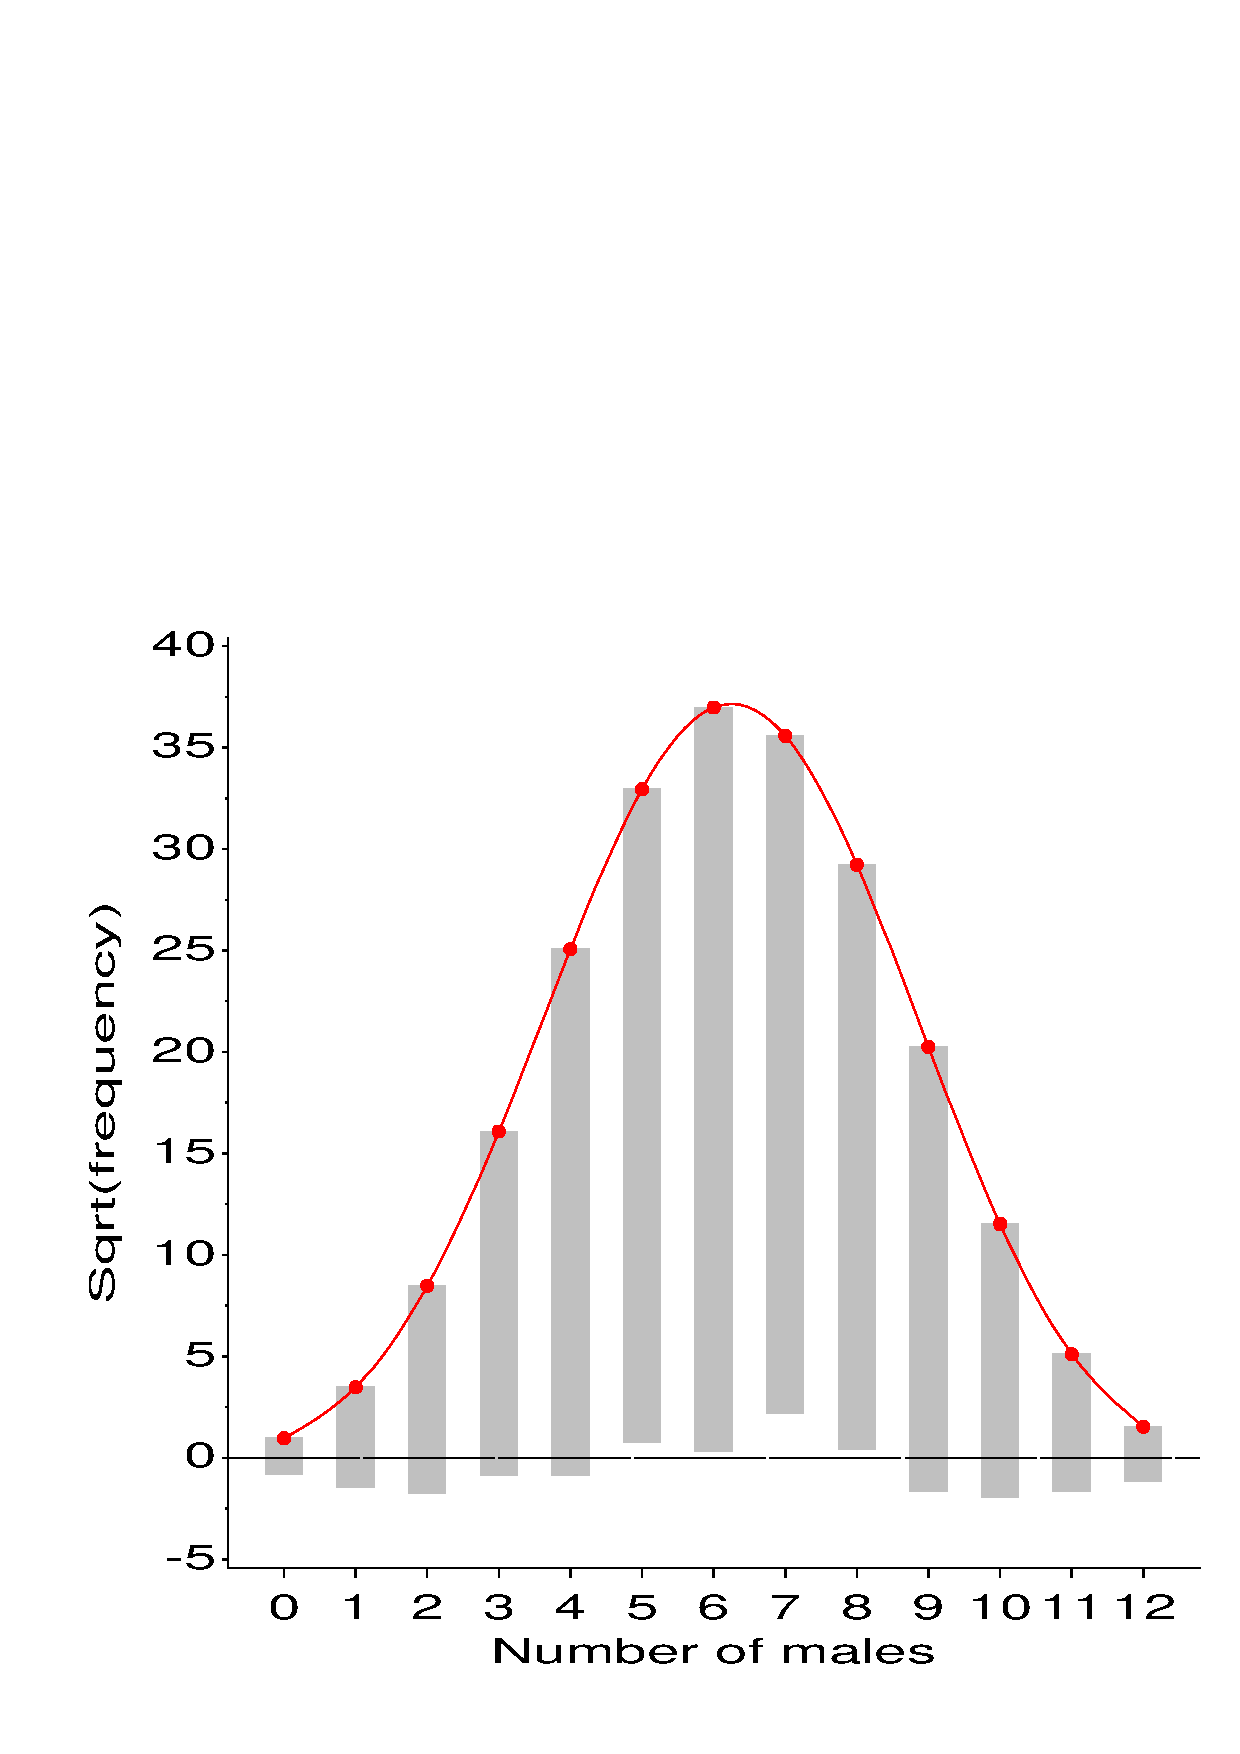
\includegraphics[width=1\linewidth]{saxony}\graphicsfile{ch2/fig/saxony.eps}{}
 \end{minipage}%
 \hfill
 \begin{minipage}[c]{.33\linewidth}
  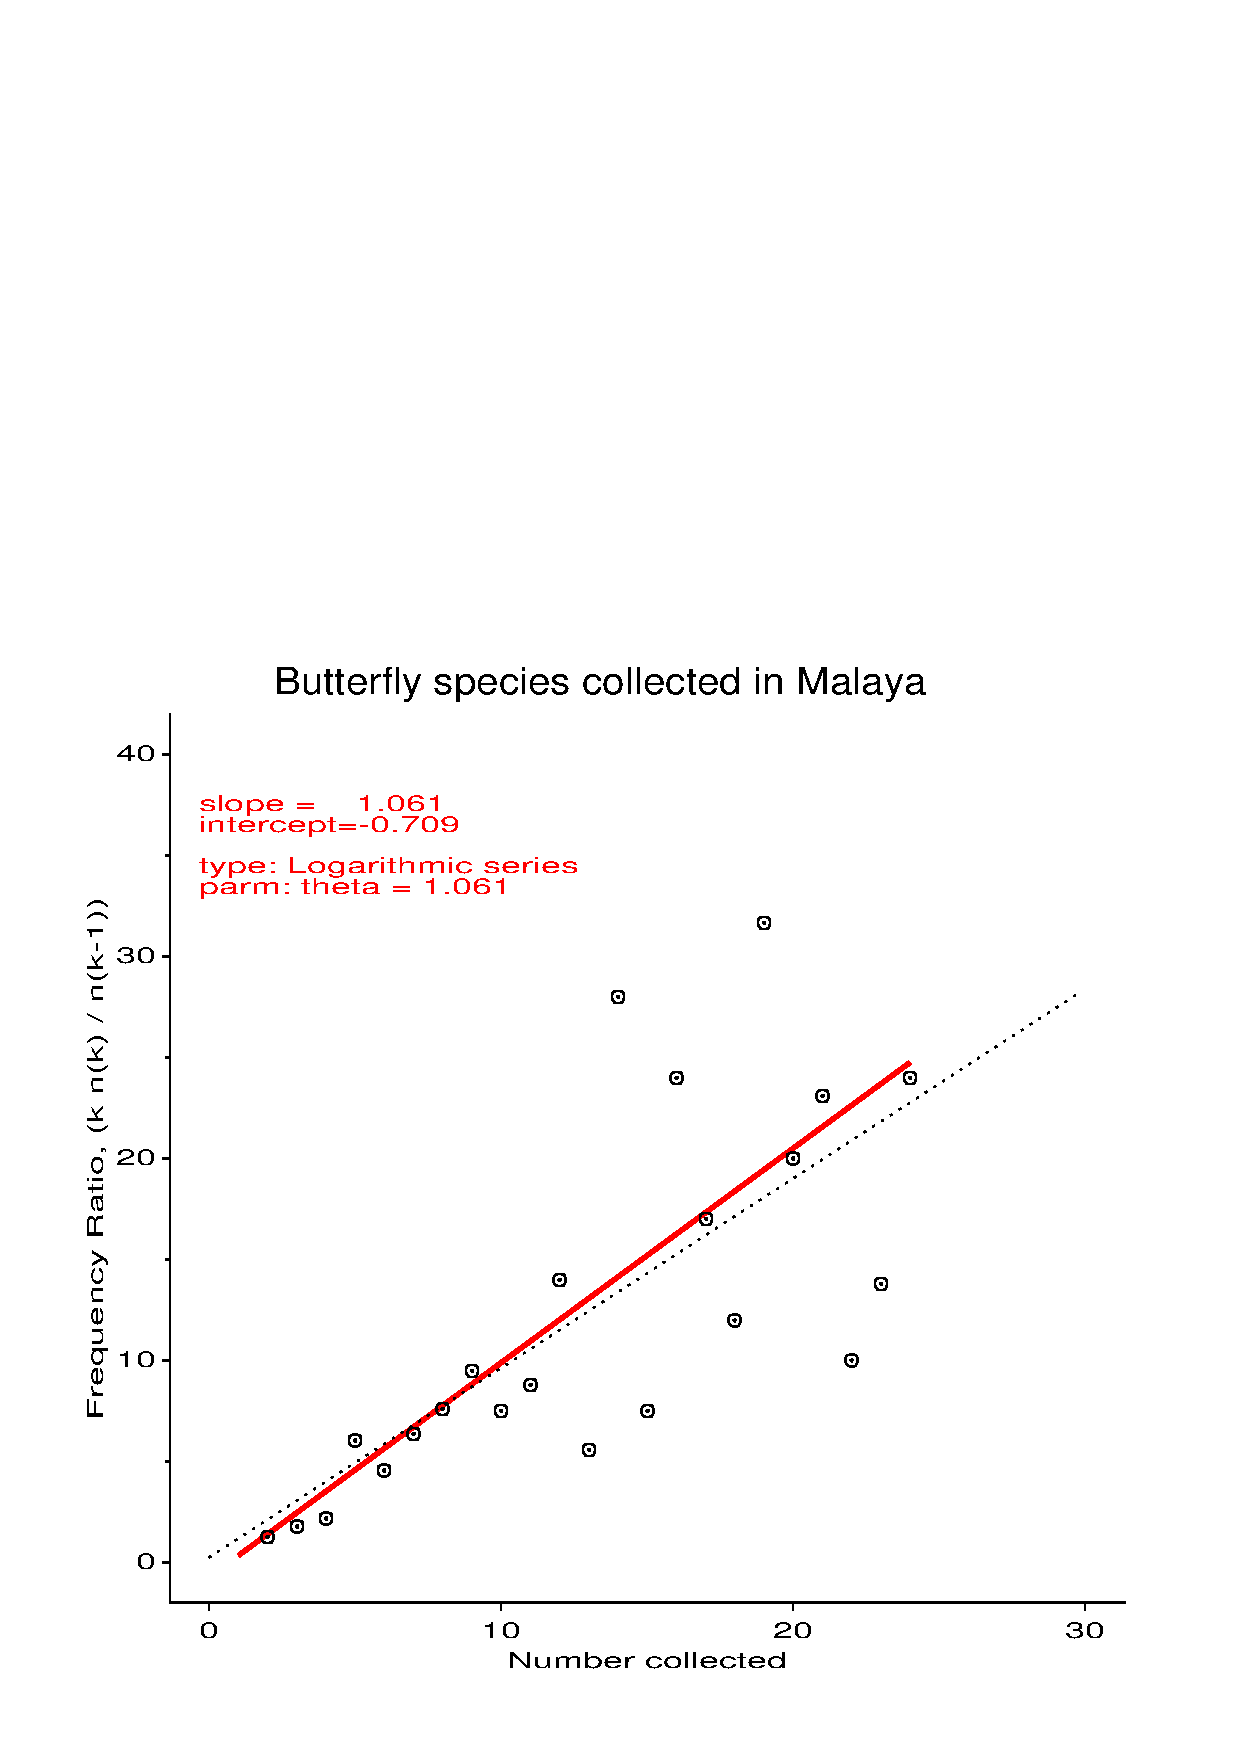
\includegraphics[width=1\linewidth]{orddemo3}\graphicsfile{ch2/fig/orddemo3.eps}{}
 \end{minipage}
 \hfill
 \begin{minipage}[c]{.33\linewidth}
  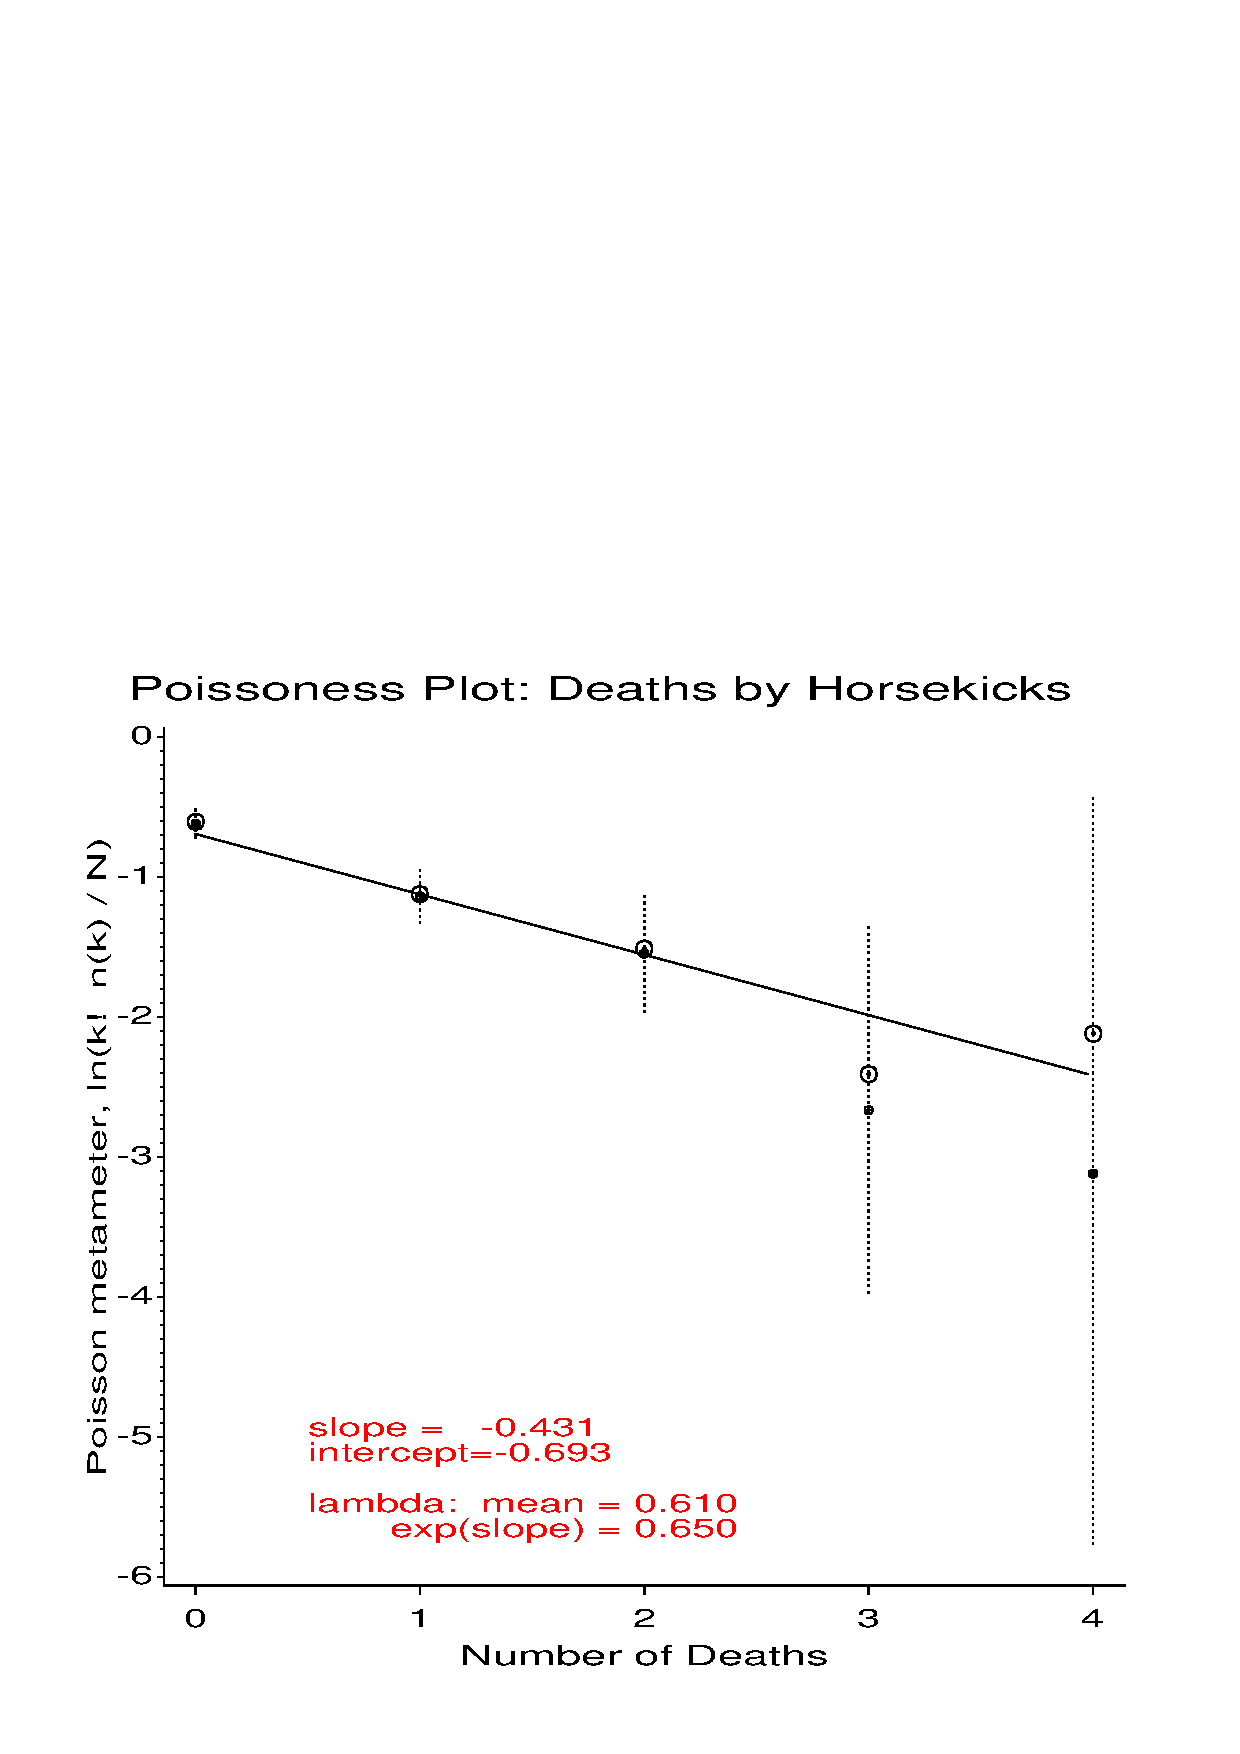
\includegraphics[width=1\linewidth]{poisdemo1}\graphicsfile{ch2/fig/poisdemo1.eps}{}
 \end{minipage}
\end{center}

   %% visual contents images

\chapterprelude{
Creating and manipulating categorical data sets requires
some skills and techniques in \R beyond those ordinarily used
for quantitative data. This chapter illustrates these for the
main formats for categorical data: case form, frequency form
and table form.
}

Categorical data can be represented as data sets
in various formats:
case form, frequency form, and table form.  This chapter
describes and illustrates the skills and techniques in \R
needed to input, create and manipulate \R data objects
to represent categorical data, and convert these from one
form to another for the purposes of statistical analysis
and visualization which are the subject of the remainder of the book.

As mentioned earlier, this book assumes that you have at least a
basic knowledge of the \R language and environment, including
interacting with the \R console (Rgui for Windows, R.app for Mac OS X)
or some other graphical user interface (e.g., R Studio),
loading and using \R functions in packages (e.g., \code{library(vcd)})
getting help for these from \R (e.g., \code{help(matrix)}), etc.
This chapter is therefore devoted
to covering those topics beyond such basic skills needed in the book.%
\footnote{
Some excellent introductory treatments of \R are:
\citet[\C 2]{FoxWeisberg:2011}, ...
Tom Short's \emph{R Reference Card}, \url{http://cran.us.r-project.org/doc/contrib/Short-refcard.pdf} is a handy 4-page summary of the main functions.
The web sites
Quick-R \url{http://www.statmethods.net/} and
Cookbook for R \url{http://www.cookbook-r.com/}
provide very helpful examples, organized by topics and tasks.
}


\section{Working with \R data: vectors, matrices, arrays and data frames}\label{sec:Rdata}

\R has a wide variety of data structures for storing, manipulating and
calculating with data.  Among these, vectors, matrices, arrays and
data frames are most important for the material in this book.

In \R, a \term{vector} is a collection of values, like numbers, character strings, logicals (\code{TRUE, FALSE})
or dates, and often correspond to a variable in some analysis.
Matrices are rectangular arrays like a traditional table, composed of vectors in their columns
or rows.
Arrays add additional dimensions, so that, for example, a 3-way table can be represented
as composed of rows, columns and layers.
An important consideration is that the values in vectors,
matrices and arrays must all be of the same \emph{mode}, e.g., numbers or character strings.
A \term{data frame} is a rectangular table, like a traditional data set in other
statistical environments, and composed of rows and columns like a matrix,
but allowing variables (columns) of different types. These data structures and the types of
data they can contain are illustrated in \figref{fig:datatypes}. A more general
data structure is a \emph{list}, a generic vector which can contain
any other types of objects.

\begin{figure}
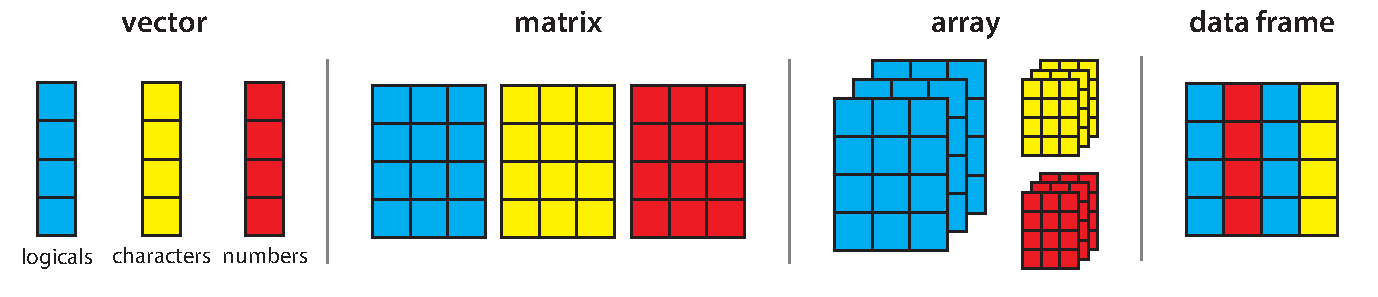
\includegraphics[width=\textwidth]{ch02/fig/datatypes2}
\caption[Principal data structures and data types in R]{Principal data structures and data types in \R. Colors
 represent different data types: numeric, character, logical. }
\label{fig:datatypes}
\end{figure}
\subsection{Vectors}
The simplest data structure in \R is a \term{vector}, a one-dimensional
collection of elements of the same type. An easy way to create a vector is with
the \func{c}, which combines its arguments.  The following examples create
and print vectors of length 4, containing numbers, character strings and
logical values respectively:

\begin{knitrout}
\definecolor{shadecolor}{rgb}{1, 0.961, 0.933}\color{fgcolor}\begin{kframe}
\begin{alltt}
\hlkwd{c}\hlstd{(}\hlnum{17}\hlstd{,} \hlnum{20}\hlstd{,} \hlnum{15}\hlstd{,} \hlnum{40}\hlstd{)}
\end{alltt}
\begin{verbatim}
## [1] 17 20 15 40
\end{verbatim}
\begin{alltt}
\hlkwd{c}\hlstd{(}\hlstr{"female"}\hlstd{,} \hlstr{"male"}\hlstd{,} \hlstr{"female"}\hlstd{,} \hlstr{"male"}\hlstd{)}
\end{alltt}
\begin{verbatim}
## [1] "female" "male"   "female" "male"
\end{verbatim}
\begin{alltt}
\hlkwd{c}\hlstd{(}\hlnum{TRUE}\hlstd{,} \hlnum{TRUE}\hlstd{,} \hlnum{FALSE}\hlstd{,} \hlnum{FALSE}\hlstd{)}
\end{alltt}
\begin{verbatim}
## [1]  TRUE  TRUE FALSE FALSE
\end{verbatim}
\end{kframe}
\end{knitrout}

To store these values in variables, \R uses the assignment operator (\code{<-})
or equals sign (\code{=}). This creates a variable named on the left-hand side.
An assignment doesn't print the result, but a bare expression does, so you can
assign and print by surrounding the assignment with \code{()}.

\begin{knitrout}
\definecolor{shadecolor}{rgb}{1, 0.961, 0.933}\color{fgcolor}\begin{kframe}
\begin{alltt}
\hlstd{count} \hlkwb{<-} \hlkwd{c}\hlstd{(}\hlnum{17}\hlstd{,} \hlnum{20}\hlstd{,} \hlnum{15}\hlstd{,} \hlnum{40}\hlstd{)}                       \hlcom{# assign}
\hlstd{count}                                            \hlcom{# print}
\end{alltt}
\begin{verbatim}
## [1] 17 20 15 40
\end{verbatim}
\begin{alltt}
\hlstd{(sex} \hlkwb{<-} \hlkwd{c}\hlstd{(}\hlstr{"female"}\hlstd{,} \hlstr{"male"}\hlstd{,} \hlstr{"female"}\hlstd{,} \hlstr{"male"}\hlstd{))}   \hlcom{# both}
\end{alltt}
\begin{verbatim}
## [1] "female" "male"   "female" "male"
\end{verbatim}
\begin{alltt}
\hlstd{(passed} \hlkwb{<-} \hlkwd{c}\hlstd{(}\hlnum{TRUE}\hlstd{,} \hlnum{TRUE}\hlstd{,} \hlnum{FALSE}\hlstd{,} \hlnum{FALSE}\hlstd{))}
\end{alltt}
\begin{verbatim}
## [1]  TRUE  TRUE FALSE FALSE
\end{verbatim}
\end{kframe}
\end{knitrout}

Other useful functions for creating vectors are:
\begin{itemize*}
  \item The \code{:} operator for generating consecutive integer sequences, e.g.,
  \code{1:10} gives the integers 1 to 10.  The \func{seq} function is more general, taking the forms
\code{seq(from, to)},
\code{seq(from, to, by= )}, and
\code{seq(from, to, length= )} where the optional argument \code{by} specifies the interval between adjacent values and \code{length} gives the desired length of the
result.

  \item The \func{rep} function generates repeated sequences, replicating
  its first argument (which may be a vector) a given number of \code{times},
  to a given \code{length} or \code{each} a given multiple.
\end{itemize*}

\begin{knitrout}
\definecolor{shadecolor}{rgb}{1, 0.961, 0.933}\color{fgcolor}\begin{kframe}
\begin{alltt}
\hlkwd{seq}\hlstd{(}\hlnum{10}\hlstd{,} \hlnum{100}\hlstd{,} \hlkwc{by}\hlstd{=}\hlnum{10}\hlstd{)}      \hlcom{# give interval}
\end{alltt}
\begin{verbatim}
##  [1]  10  20  30  40  50  60  70  80  90 100
\end{verbatim}
\begin{alltt}
\hlkwd{seq}\hlstd{(}\hlnum{0}\hlstd{,} \hlnum{1}\hlstd{,} \hlkwc{length}\hlstd{=}\hlnum{11}\hlstd{)}     \hlcom{# give length}
\end{alltt}
\begin{verbatim}
##  [1] 0.0 0.1 0.2 0.3 0.4 0.5 0.6 0.7 0.8 0.9 1.0
\end{verbatim}
\begin{alltt}
\hlstd{(sex} \hlkwb{<-} \hlkwd{rep}\hlstd{(}\hlkwd{c}\hlstd{(}\hlstr{"female"}\hlstd{,} \hlstr{"male"}\hlstd{),} \hlkwc{times}\hlstd{=}\hlnum{2}\hlstd{))}
\end{alltt}
\begin{verbatim}
## [1] "female" "male"   "female" "male"
\end{verbatim}
\begin{alltt}
\hlstd{(sex} \hlkwb{<-} \hlkwd{rep}\hlstd{(}\hlkwd{c}\hlstd{(}\hlstr{"female"}\hlstd{,} \hlstr{"male"}\hlstd{),} \hlkwc{length.out}\hlstd{=}\hlnum{4}\hlstd{))}  \hlcom{# same}
\end{alltt}
\begin{verbatim}
## [1] "female" "male"   "female" "male"
\end{verbatim}
\begin{alltt}
\hlstd{(passed} \hlkwb{<-} \hlkwd{rep}\hlstd{(}\hlkwd{c}\hlstd{(}\hlnum{TRUE}\hlstd{,} \hlnum{FALSE}\hlstd{),} \hlkwc{each}\hlstd{=}\hlnum{2}\hlstd{))}
\end{alltt}
\begin{verbatim}
## [1]  TRUE  TRUE FALSE FALSE
\end{verbatim}
\end{kframe}
\end{knitrout}

\subsection{Matrices}
A \term{matrix} is a two-dimensional array of elements of the same type composed
in a rectangular array of rows and columns. Matrices can be created by the function
\code{matrix(values, nrow, ncol)}, which takes the reshapes the elements in
the first argument (\code{values}) to a matrix with \code{nrow} rows and
\code{ncol} columns. By default, the elements are filled in columnwise, unless
the optional argument \code{byrow=TRUE} is given.

\begin{knitrout}
\definecolor{shadecolor}{rgb}{1, 0.961, 0.933}\color{fgcolor}\begin{kframe}
\begin{alltt}
\hlstd{(matA} \hlkwb{<-} \hlkwd{matrix}\hlstd{(}\hlnum{1}\hlopt{:}\hlnum{8}\hlstd{,} \hlkwc{nrow}\hlstd{=}\hlnum{2}\hlstd{,} \hlkwc{ncol}\hlstd{=}\hlnum{4}\hlstd{))}
\end{alltt}
\begin{verbatim}
##      [,1] [,2] [,3] [,4]
## [1,]    1    3    5    7
## [2,]    2    4    6    8
\end{verbatim}
\begin{alltt}
\hlstd{(matB} \hlkwb{<-} \hlkwd{matrix}\hlstd{(}\hlnum{1}\hlopt{:}\hlnum{8}\hlstd{,} \hlkwc{nrow}\hlstd{=}\hlnum{2}\hlstd{,} \hlkwc{ncol}\hlstd{=}\hlnum{4}\hlstd{,} \hlkwc{byrow}\hlstd{=}\hlnum{TRUE}\hlstd{))}
\end{alltt}
\begin{verbatim}
##      [,1] [,2] [,3] [,4]
## [1,]    1    2    3    4
## [2,]    5    6    7    8
\end{verbatim}
\begin{alltt}
\hlstd{(matC} \hlkwb{<-} \hlkwd{matrix}\hlstd{(}\hlnum{1}\hlopt{:}\hlnum{4}\hlstd{,} \hlkwc{nrow}\hlstd{=}\hlnum{2}\hlstd{,} \hlkwc{ncol}\hlstd{=}\hlnum{4}\hlstd{))}
\end{alltt}
\begin{verbatim}
##      [,1] [,2] [,3] [,4]
## [1,]    1    3    1    3
## [2,]    2    4    2    4
\end{verbatim}
\end{kframe}
\end{knitrout}
\noindent The last example illustrates that the values in the first argument are recycled
as necessary to fill the given number of rows and columns.

All matrices have a dimensions attribute, a vector of length two giving the number
of rows and columns, retrieved with the function \func{dim}. Labels for the rows and
columns can be assigned using \func{dimnames},%
\footnote{
The \code{dimnames} can also be specified as an optional argument to \func{matrix}.
}
which takes a list of two vectors for the
row names and column names respectively. To see the structure of a matrix
(or any other \R object) and its attributes, I frequently use the \func{str} function,
as shown in the example below.

\begin{knitrout}
\definecolor{shadecolor}{rgb}{1, 0.961, 0.933}\color{fgcolor}\begin{kframe}
\begin{alltt}
\hlkwd{dim}\hlstd{(matA)}
\end{alltt}
\begin{verbatim}
## [1] 2 4
\end{verbatim}
\begin{alltt}
\hlkwd{str}\hlstd{(matA)}
\end{alltt}
\begin{verbatim}
##  int [1:2, 1:4] 1 2 3 4 5 6 7 8
\end{verbatim}
\begin{alltt}
\hlkwd{dimnames}\hlstd{(matA)} \hlkwb{<-} \hlkwd{list}\hlstd{(}\hlkwd{c}\hlstd{(}\hlstr{"M"}\hlstd{,}\hlstr{"F"}\hlstd{), LETTERS[}\hlnum{1}\hlopt{:}\hlnum{4}\hlstd{])}
\hlstd{matA}
\end{alltt}
\begin{verbatim}
##   A B C D
## M 1 3 5 7
## F 2 4 6 8
\end{verbatim}
\begin{alltt}
\hlkwd{str}\hlstd{(matA)}
\end{alltt}
\begin{verbatim}
##  int [1:2, 1:4] 1 2 3 4 5 6 7 8
##  - attr(*, "dimnames")=List of 2
##   ..$ : chr [1:2] "M" "F"
##   ..$ : chr [1:4] "A" "B" "C" "D"
\end{verbatim}
\end{kframe}
\end{knitrout}
Additionally, names for the row and column \emph{variables} themselves can also be assigned in the
\code{dimnames} call by giving each dimension vector a name.
\begin{knitrout}
\definecolor{shadecolor}{rgb}{1, 0.961, 0.933}\color{fgcolor}\begin{kframe}
\begin{alltt}
\hlkwd{dimnames}\hlstd{(matA)} \hlkwb{<-} \hlkwd{list}\hlstd{(}\hlkwc{sex}\hlstd{=}\hlkwd{c}\hlstd{(}\hlstr{"M"}\hlstd{,}\hlstr{"F"}\hlstd{),} \hlkwc{group}\hlstd{=LETTERS[}\hlnum{1}\hlopt{:}\hlnum{4}\hlstd{])}
\hlstd{matA}
\end{alltt}
\begin{verbatim}
##    group
## sex A B C D
##   M 1 3 5 7
##   F 2 4 6 8
\end{verbatim}
\begin{alltt}
\hlkwd{str}\hlstd{(matA)}
\end{alltt}
\begin{verbatim}
##  int [1:2, 1:4] 1 2 3 4 5 6 7 8
##  - attr(*, "dimnames")=List of 2
##   ..$ sex  : chr [1:2] "M" "F"
##   ..$ group: chr [1:4] "A" "B" "C" "D"
\end{verbatim}
\end{kframe}
\end{knitrout}

Matrices can also be created or enlarged by ``binding'' vectors or matrices together
by rows or columns:
\begin{itemize*}
  \item \code{rbind(a, b, c)} creates a matrix with the vectors \code{a}, \code{b} and \code{c} as its rows, recycling the elements as necessary to the length of the longest one.
  \item \code{cbind(a, b, c)} creates a matrix with the vectors \code{a}, \code{b} and \code{c} as its columns.
  \item \code{rbind(mat, a, b, ...)} and \code{cbind(mat, a, b, ...)} add additional
  rows (columns) to a matrix \code{mat}, recycling or subsetting the elements in the
  vectors to conform with the size of the matrix.
\end{itemize*}

\begin{knitrout}
\definecolor{shadecolor}{rgb}{1, 0.961, 0.933}\color{fgcolor}\begin{kframe}
\begin{alltt}
\hlkwd{rbind}\hlstd{(matA,} \hlkwd{c}\hlstd{(}\hlnum{10}\hlstd{,}\hlnum{20}\hlstd{))}
\end{alltt}
\begin{verbatim}
##    A  B  C  D
## M  1  3  5  7
## F  2  4  6  8
##   10 20 10 20
\end{verbatim}
\begin{alltt}
\hlkwd{cbind}\hlstd{(matA,} \hlkwd{c}\hlstd{(}\hlnum{10}\hlstd{,}\hlnum{20}\hlstd{))}
\end{alltt}
\begin{verbatim}
##   A B C D   
## M 1 3 5 7 10
## F 2 4 6 8 20
\end{verbatim}
\end{kframe}
\end{knitrout}

\subsection{Arrays}
Higher-dimensional arrays are less frequently encountered in traditional data analysis,
but they are of great use for categorical data, where frequency tables of three or more
variables can be naturally represented as arrays, with one dimension for each
table variable.

The function \code{array(values, dim)} takes the elements in \code{values} and
reshapes these into an array whose dimensions are given in the vector \code{dim}.
The number of dimensions is the length of \code{dim}.  As with matrices, the
elements are filled in with the first dimension (rows) varying most rapidly,
then by the second dimension (columns) and so on for all further dimensions,
which can be considered as layers.
A matrix is just the special case of an array with two dimensions.

\begin{knitrout}
\definecolor{shadecolor}{rgb}{1, 0.961, 0.933}\color{fgcolor}\begin{kframe}
\begin{alltt}
\hlstd{(arrayA} \hlkwb{<-} \hlkwd{array}\hlstd{(}\hlnum{1}\hlopt{:}\hlnum{16}\hlstd{,} \hlkwc{dim}\hlstd{=}\hlkwd{c}\hlstd{(}\hlnum{2}\hlstd{,} \hlnum{4}\hlstd{,} \hlnum{2}\hlstd{)))}     \hlcom{# 2 rows, 4 columns, 2 layers}
\end{alltt}
\begin{verbatim}
## , , 1
## 
##      [,1] [,2] [,3] [,4]
## [1,]    1    3    5    7
## [2,]    2    4    6    8
## 
## , , 2
## 
##      [,1] [,2] [,3] [,4]
## [1,]    9   11   13   15
## [2,]   10   12   14   16
\end{verbatim}
\begin{alltt}
\hlkwd{str}\hlstd{(arrayA)}
\end{alltt}
\begin{verbatim}
##  int [1:2, 1:4, 1:2] 1 2 3 4 5 6 7 8 9 10 ...
\end{verbatim}
\begin{alltt}
\hlstd{(arrayB} \hlkwb{<-} \hlkwd{array}\hlstd{(}\hlnum{1}\hlopt{:}\hlnum{16}\hlstd{,} \hlkwc{dim}\hlstd{=}\hlkwd{c}\hlstd{(}\hlnum{2}\hlstd{,} \hlnum{8}\hlstd{)))}        \hlcom{# 2 rows, 8 columns}
\end{alltt}
\begin{verbatim}
##      [,1] [,2] [,3] [,4] [,5] [,6] [,7] [,8]
## [1,]    1    3    5    7    9   11   13   15
## [2,]    2    4    6    8   10   12   14   16
\end{verbatim}
\begin{alltt}
\hlkwd{str}\hlstd{(arrayB)}
\end{alltt}
\begin{verbatim}
##  int [1:2, 1:8] 1 2 3 4 5 6 7 8 9 10 ...
\end{verbatim}
\end{kframe}
\end{knitrout}
In the same way that we can assign labels to the rows, columns and variables
in matrices, we can assign these attributes to \code{dimnames(arrayA)}, or
include this information in a \code{dimnames=} argument to \func{array}.

\begin{knitrout}
\definecolor{shadecolor}{rgb}{1, 0.961, 0.933}\color{fgcolor}\begin{kframe}
\begin{alltt}
\hlkwd{dimnames}\hlstd{(arrayA)} \hlkwb{<-} \hlkwd{list}\hlstd{(}\hlkwc{sex}\hlstd{=}\hlkwd{c}\hlstd{(}\hlstr{"M"}\hlstd{,} \hlstr{"F"}\hlstd{),}
                         \hlkwc{group}\hlstd{=letters[}\hlnum{1}\hlopt{:}\hlnum{4}\hlstd{],}
                         \hlkwc{time}\hlstd{=}\hlkwd{c}\hlstd{(}\hlstr{"Pre"}\hlstd{,} \hlstr{"Post"}\hlstd{))}
\hlstd{arrayA}
\end{alltt}
\begin{verbatim}
## , , time = Pre
## 
##    group
## sex a b c d
##   M 1 3 5 7
##   F 2 4 6 8
## 
## , , time = Post
## 
##    group
## sex  a  b  c  d
##   M  9 11 13 15
##   F 10 12 14 16
\end{verbatim}
\begin{alltt}
\hlkwd{str}\hlstd{(arrayA)}
\end{alltt}
\begin{verbatim}
##  int [1:2, 1:4, 1:2] 1 2 3 4 5 6 7 8 9 10 ...
##  - attr(*, "dimnames")=List of 3
##   ..$ sex  : chr [1:2] "M" "F"
##   ..$ group: chr [1:4] "a" "b" "c" "d"
##   ..$ time : chr [1:2] "Pre" "Post"
\end{verbatim}
\end{kframe}
\end{knitrout}
Arrays in \R can contain any single type of elements--- numbers,
character strings, logicals.  \R also has a variety of functions
(e.g., \func{table}, \func{xtabs})
for creating and manipulating \class{table} objects, which are
specialized forms of matrices and arrays containing integer
frequencies in a contingency table. These are discussed in more
detail below (\secref{sec:table}).

\subsection{data frames}\label{sec:data-frames}
Data frames are the most commonly used form of data in \R and more
general than matrices in that they can contain columns of different types.
For statistical modeling, data frames play a special role, in that
many modeling functions are designed to take a data frame as a
\code{data=} argument, and then find the variables mentioned within
that data frame. Another distinguishing feature is that discrete variables
(columns) like character strings \code{("M", "F")} or integers \code{(1, 2, 3)}
in data frames can be represented as \term{factor}s, which simplifies
many statistical and graphical methods.

A data frame can be created using keyboard input
with the \func{data.frame} function, applied to a list of objects,
\code{data.frame(a, b, c, ...)}, each of which can be a vector, matrix or another
data frame, but typically all containing the same number of rows.
This works roughly like \func{cbind}, collecting the arguments as columns
in the result.

The following example generates \code{n=100} random observations on
three discrete factor variables, \code{A, B, sex}, and a numeric
variable, \code{age}.  As constructed, all of these are
statistically independent, since none depends on any of the others.
The function \func{sample}
is used here to generate \code{n} random samples from the
first argument allowing replacement (\code{rep=TRUE}).
Finally, all four variables are combined into the data frame
\code{mydata}.


\begin{knitrout}
\definecolor{shadecolor}{rgb}{1, 0.961, 0.933}\color{fgcolor}\begin{kframe}
\begin{alltt}
\hlkwd{set.seed}\hlstd{(}\hlnum{12345}\hlstd{)}   \hlcom{# reproducibility}
\hlstd{n}\hlkwb{=}\hlnum{100}
\hlstd{A} \hlkwb{<-} \hlkwd{factor}\hlstd{(}\hlkwd{sample}\hlstd{(}\hlkwd{c}\hlstd{(}\hlstr{"a1"}\hlstd{,}\hlstr{"a2"}\hlstd{), n,} \hlkwc{rep}\hlstd{=}\hlnum{TRUE}\hlstd{))}
\hlstd{B} \hlkwb{<-} \hlkwd{factor}\hlstd{(}\hlkwd{sample}\hlstd{(}\hlkwd{c}\hlstd{(}\hlstr{"b1"}\hlstd{,}\hlstr{"b2"}\hlstd{), n,} \hlkwc{rep}\hlstd{=}\hlnum{TRUE}\hlstd{))}
\hlstd{sex} \hlkwb{<-} \hlkwd{factor}\hlstd{(}\hlkwd{sample}\hlstd{(}\hlkwd{c}\hlstd{(}\hlstr{"M"}\hlstd{,} \hlstr{"F"}\hlstd{), n,} \hlkwc{rep}\hlstd{=}\hlnum{TRUE}\hlstd{))}
\hlstd{age} \hlkwb{<-} \hlkwd{round}\hlstd{(}\hlkwd{rnorm}\hlstd{(n,} \hlkwc{mean}\hlstd{=}\hlnum{30}\hlstd{,} \hlkwc{sd}\hlstd{=}\hlnum{5}\hlstd{))}
\hlstd{mydata} \hlkwb{<-} \hlkwd{data.frame}\hlstd{(A, B, sex, age)}
\hlkwd{head}\hlstd{(mydata,}\hlnum{5}\hlstd{)}
\end{alltt}
\begin{verbatim}
##    A  B sex age
## 1 a2 b1   F  22
## 2 a2 b2   F  33
## 3 a2 b2   M  31
## 4 a2 b2   F  26
## 5 a1 b2   F  29
\end{verbatim}
\begin{alltt}
\hlkwd{str}\hlstd{(mydata)}
\end{alltt}
\begin{verbatim}
## 'data.frame':	100 obs. of  4 variables:
##  $ A  : Factor w/ 2 levels "a1","a2": 2 2 2 2 1 1 1 2 2 2 ...
##  $ B  : Factor w/ 2 levels "b1","b2": 1 2 2 2 2 2 2 2 1 1 ...
##  $ sex: Factor w/ 2 levels "F","M": 1 1 2 1 1 1 2 2 1 1 ...
##  $ age: num  22 33 31 26 29 29 38 28 30 27 ...
\end{verbatim}
\end{kframe}
\end{knitrout}

For real data sets, it is usually most convenient to read these into \R
from external files, and this is easiest using plain text (ASCII) files
with one line per observation and fields separated by commas (or tabs),
and with a first header line giving the variable names-- called
\emph{comma-separated} or CSV format.
If your data is in the form of Excel, SAS, SPSS or other file format,
you can almost always export that data to CSV format first.%
\footnote{
The \Rpackage{foreign} contains specialized functions to \emph{directly} read
data stored by Minitab, SAS, SPSS, Stata, Systat and other software.
There are also a number of packages for reading (and writing)
Excel spreadsheets directly (\pkg{gdata}, \pkg{XLConnect}, \pkg{xlsx}).
The \R manual, \emph{R Data Import/Export} covers many other variations,
including data in relational data bases.
}

The function \func{read.table} has many options to control the details
of how the data are read and converted to variables in the data frame.
Among these some important options are:
\begin{description*}
  \item [\code{header}] indicates whether the first line contains
variable names. The default is \code{FALSE} unless the first line contains one fewer field
than the number of columns;
  \item[\code{sep}] (default: \code{""} meaning white space, i.e., one or more spaces, tabs or newlines) specifies the separator character between fields;
  \item[\code{stringsAsFactors}] (default: \code{TRUE}) determines whether character string variables should be converted to factors;
  \item[\code{na.strings}] (default: \code{"NA"}) one or more strings which are interpreted
  as missing data values (\code{NA});
\end{description*}
For delimited files, \func{read.csv} and \func{read.delim} are convenient wrappers
to \func{read.table}, with default values \code{sep=","} and \code{sep="\t"}
respectively, and
\code{header=TRUE}.

\begin{Example}[ch2-arth-csv]{Arthritis treatment}

The file \code{Arthritis.csv} contains data in CSV format
from \citet{KochEdwards:88}, representing
a double-blind clinical trial investigating a new treatment for rheumatoid arthritis with 84 patients. The first (``header'') line gives the variable names.  Some of the
lines in the file are shown below, with \code{...} representing omitted lines:
{\small
\renewcommand{\baselinestretch}{.85}
%<<arth-csv, eval=FALSE, results='asis'>>=
\begin{verbatim}
ID,Treatment,Sex,Age,Improved
57,Treated,Male,27,Some
46,Treated,Male,29,None
77,Treated,Male,30,None
17,Treated,Male,32,Marked
 ...
42,Placebo,Female,66,None
15,Placebo,Female,66,Some
71,Placebo,Female,68,Some
1,Placebo,Female,74,Marked
\end{verbatim}
%@
}
We read this into \R using \func{read.csv} as shown below, using all the
default options:
\begin{knitrout}\footnotesize
\definecolor{shadecolor}{rgb}{1, 0.961, 0.933}\color{fgcolor}\begin{kframe}
\begin{alltt}
\hlstd{Arthritis} \hlkwb{<-} \hlkwd{read.csv}\hlstd{(}\hlstr{"ch02/Arthritis.csv"}\hlstd{)}
\hlkwd{str}\hlstd{(Arthritis)}
\end{alltt}
\begin{verbatim}
## 'data.frame':	84 obs. of  5 variables:
##  $ ID       : int  57 46 77 17 36 23 75 39 33 55 ...
##  $ Treatment: Factor w/ 2 levels "Placebo","Treated": 2 2 2 2 2 2 2 2 2 2 ...
##  $ Sex      : Factor w/ 2 levels "Female","Male": 2 2 2 2 2 2 2 2 2 2 ...
##  $ Age      : int  27 29 30 32 46 58 59 59 63 63 ...
##  $ Improved : Factor w/ 3 levels "Marked","None",..: 3 2 2 1 1 1 2 1 2 2 ...
\end{verbatim}
\end{kframe}
\end{knitrout}
Note that the character variables \var{Treatment}, \var{Sex} and \var{Improved}
were converted to factors, and the levels of those variables were
ordered \emph{alphabetically}.  This often doesn't matter much for binary variables,
but here, the response variable, \var{Improved} has levels
that should be considered \emph{ordered},
as \code{"None", "Some", "Marked"}.  We can correct this here by
re-assigning \code{Arthritis$Improved} using \func{ordered}.
The topic of re-ordering variables and levels in categorical data is
considered in more detail in \secref{sec:ordered}.

\begin{knitrout}
\definecolor{shadecolor}{rgb}{1, 0.961, 0.933}\color{fgcolor}\begin{kframe}
\begin{alltt}
\hlkwd{levels}\hlstd{(Arthritis}\hlopt{$}\hlstd{Improved)}
\end{alltt}
\begin{verbatim}
## [1] "Marked" "None"   "Some"
\end{verbatim}
\begin{alltt}
\hlstd{Arthritis}\hlopt{$}\hlstd{Improved} \hlkwb{<-} \hlkwd{ordered}\hlstd{(Arthritis}\hlopt{$}\hlstd{Improved,}
                              \hlkwc{levels}\hlstd{=}\hlkwd{c}\hlstd{(}\hlstr{"None"}\hlstd{,} \hlstr{"Some"}\hlstd{,} \hlstr{"Marked"}\hlstd{))}
\end{alltt}
\end{kframe}
\end{knitrout}

\end{Example}

\section{Forms of categorical data: case form, frequency form and table form}\label{sec:forms}
As we saw in \chref{ch:intro}, categorical data can be represented as ordinary data sets
in case form, but the discrete nature of factors or stratifying variables allows the same
information to be represented more compactly in summarized form with a frequency
variable for each cell of factor combinations, or in tables.
Consequently, we sometimes
find data created or presented in one form (e.g., a spreadsheet data set, a two-way
table of frequencies) and want to input that into \R.  Once we have the data in \R,
it is often necessary to manipulate the data into some other form for the purposes
of statistical analysis, visualizing results and our own presentation.
It is useful to understand the three main forms of categorical data in \R and how
to work with them for our purposes.

\subsection{Case form}
Categorical data in case form are simply data frames, with one or more discrete
classifying variables or response variables, most conveniently represented as factors or ordered factors.  In case form, the data set can also contain numeric variables
(covariates or other response variables), that cannot be accommodated in other
forms.

As with any data frame, \code{X}, you can access or compute with its attributes using \code{nrow(X)} for the number of observations,
\code{ncol(X)} for the number of variables,
\code{names(X)} or \code{colnames(X)} for the variable names and
so forth.

\begin{Example}[ch2-arth]{Arthritis treatment}

The \data{Arthritis} data is available in case form in the \pkg{vcd} package.
There are two explanatory factors: \code{Treatment} and \code{Sex}. \code{Age}
is a numeric covariate, and \code{Improved} is the response--- an ordered factor,
with levels
%\code{paste(levels(Arthritis$Improved),collapse=' < ')}.
\code{"None" < "Some" < "Marked"}.
Excluding \code{Age}, we would have
a $2 \times 2 \times 3$ contingency table for \code{Treatment}, \code{Sex} and \code{Improved}.
\begin{knitrout}\footnotesize
\definecolor{shadecolor}{rgb}{1, 0.961, 0.933}\color{fgcolor}\begin{kframe}
\begin{alltt}
\hlkwd{data}\hlstd{(Arthritis,} \hlkwc{package}\hlstd{=}\hlstr{"vcd"}\hlstd{)}  \hlcom{# load the data}
\hlkwd{names}\hlstd{(Arthritis)}      \hlcom{# show the variables}
\end{alltt}
\begin{verbatim}
## [1] "ID"        "Treatment" "Sex"       "Age"       "Improved"
\end{verbatim}
\begin{alltt}
\hlkwd{str}\hlstd{(Arthritis)}        \hlcom{# show the structure}
\end{alltt}
\begin{verbatim}
## 'data.frame':	84 obs. of  5 variables:
##  $ ID       : int  57 46 77 17 36 23 75 39 33 55 ...
##  $ Treatment: Factor w/ 2 levels "Placebo","Treated": 2 2 2 2 2 2 2 2 2 2 ...
##  $ Sex      : Factor w/ 2 levels "Female","Male": 2 2 2 2 2 2 2 2 2 2 ...
##  $ Age      : int  27 29 30 32 46 58 59 59 63 63 ...
##  $ Improved : Ord.factor w/ 3 levels "None"<"Some"<..: 2 1 1 3 3 3 1 3 1 1 ...
\end{verbatim}
\begin{alltt}
\hlkwd{head}\hlstd{(Arthritis,}\hlnum{5}\hlstd{)}     \hlcom{# first 5 observations, same as Arthritis[1:5,]}
\end{alltt}
\begin{verbatim}
##   ID Treatment  Sex Age Improved
## 1 57   Treated Male  27     Some
## 2 46   Treated Male  29     None
## 3 77   Treated Male  30     None
## 4 17   Treated Male  32   Marked
## 5 36   Treated Male  46   Marked
\end{verbatim}
\end{kframe}
\end{knitrout}
\end{Example}

\subsection{Frequency form}
Data in frequency form is also a data frame, containing
one or more discrete factor variables and a frequency variable
(often called \code{Freq} or \code{count})
representing the number of basic observations in that cell.

This is an alternative representation of a table form data set considered
below.
In frequency form, the number of cells in the equivalent table
is \code{nrow{X}}, and the total number of observations
is the sum of the frequency variable, \code{sum(X$Freq)},
 \code{sum(X[,"Freq"])} or similar expression.

\begin{Example}[ch2-GSS]{General social survey}
For small frequency tables, it is often convenient to enter them in frequency form
using \func{expand.grid} for the factors and \func{c} to list the counts in a vector.
The example below, from \cite{Agresti:2002} gives results for the 1991 General Social Survey,
with respondents classified by sex and party identification.
As a table, the data look like this:
\begin{center}
\begin{tabular}{rrrr}
  \hline
    &     & party & \\
  \hline
sex & dem & indep & rep \\
  \hline
female & 279 & 73 & 225 \\
  male & 165 & 47 & 191 \\
   \hline
\end{tabular}
\end{center}


We use \func{expand.grid} to create a $6 \times 2$ matrix
containing the combinations of \code{sex} and \code{party}
with the levels for \code{sex} given first, so that this varies
most rapidly. Then,
input the frequencies in the table by columns from
left to right, and combine these two results with
\func{data.frame}.
\begin{knitrout}
\definecolor{shadecolor}{rgb}{1, 0.961, 0.933}\color{fgcolor}\begin{kframe}
\begin{alltt}
\hlcom{# Agresti (2002), table 3.11, p. 106}
\hlstd{GSS} \hlkwb{<-} \hlkwd{data.frame}\hlstd{(}
  \hlkwd{expand.grid}\hlstd{(}\hlkwc{sex}\hlstd{=}\hlkwd{c}\hlstd{(}\hlstr{"female"}\hlstd{,} \hlstr{"male"}\hlstd{),}
              \hlkwc{party}\hlstd{=}\hlkwd{c}\hlstd{(}\hlstr{"dem"}\hlstd{,} \hlstr{"indep"}\hlstd{,} \hlstr{"rep"}\hlstd{)),}
  \hlkwc{count}\hlstd{=}\hlkwd{c}\hlstd{(}\hlnum{279}\hlstd{,}\hlnum{165}\hlstd{,}\hlnum{73}\hlstd{,}\hlnum{47}\hlstd{,}\hlnum{225}\hlstd{,}\hlnum{191}\hlstd{))}
\hlstd{GSS}
\end{alltt}
\begin{verbatim}
##      sex party count
## 1 female   dem   279
## 2   male   dem   165
## 3 female indep    73
## 4   male indep    47
## 5 female   rep   225
## 6   male   rep   191
\end{verbatim}
\begin{alltt}
\hlkwd{names}\hlstd{(GSS)}
\end{alltt}
\begin{verbatim}
## [1] "sex"   "party" "count"
\end{verbatim}
\begin{alltt}
\hlkwd{str}\hlstd{(GSS)}
\end{alltt}
\begin{verbatim}
## 'data.frame':	6 obs. of  3 variables:
##  $ sex  : Factor w/ 2 levels "female","male": 1 2 1 2 1 2
##  $ party: Factor w/ 3 levels "dem","indep",..: 1 1 2 2 3 3
##  $ count: num  279 165 73 47 225 191
\end{verbatim}
\begin{alltt}
\hlkwd{sum}\hlstd{(GSS}\hlopt{$}\hlstd{count)}
\end{alltt}
\begin{verbatim}
## [1] 980
\end{verbatim}
\end{kframe}
\end{knitrout}
The last line above shows that there are 980
cases represented in the frequency table.
\end{Example}

\subsection{Table form}
Table form data is represented as a matrix, array or table object
whose elements are the frequencies in an $n$-way table.
The number of dimensions of the table is the length,
\code{length(dim(X))}, of its
\code{dim} (or \code{dimnames}) attribute, and the sizes of the
dimensions in the table are the elements of \code{dim(X)}.
The total number of observations represented is the sum of
all the frequencies, \code{sum(X)}.

\begin{Example}[ch2-hec]{Hair color and eye color}
A classic data set on frequencies of hair color, eye color and
sex is given in table form in \code{HairEyeColor} in the
\Rpackage{vcd}, reporting the frequencies of these
categories for \code{592} students in
a statistics course.
\begin{knitrout}
\definecolor{shadecolor}{rgb}{1, 0.961, 0.933}\color{fgcolor}\begin{kframe}
\begin{alltt}
\hlkwd{data}\hlstd{(HairEyeColor,} \hlkwc{package}\hlstd{=}\hlstr{"datasets"}\hlstd{)}    \hlcom{# load the data}
\hlkwd{str}\hlstd{(HairEyeColor)}                \hlcom{# show the structure}
\end{alltt}
\begin{verbatim}
##  table [1:4, 1:4, 1:2] 32 53 10 3 11 50 10 30 10 25 ...
##  - attr(*, "dimnames")=List of 3
##   ..$ Hair: chr [1:4] "Black" "Brown" "Red" "Blond"
##   ..$ Eye : chr [1:4] "Brown" "Blue" "Hazel" "Green"
##   ..$ Sex : chr [1:2] "Male" "Female"
\end{verbatim}
\begin{alltt}
\hlkwd{dim}\hlstd{(HairEyeColor)}                \hlcom{# table dimension sizes}
\end{alltt}
\begin{verbatim}
## [1] 4 4 2
\end{verbatim}
\begin{alltt}
\hlkwd{dimnames}\hlstd{(HairEyeColor)}           \hlcom{# variable and level names}
\end{alltt}
\begin{verbatim}
## $Hair
## [1] "Black" "Brown" "Red"   "Blond"
## 
## $Eye
## [1] "Brown" "Blue"  "Hazel" "Green"
## 
## $Sex
## [1] "Male"   "Female"
\end{verbatim}
\begin{alltt}
\hlkwd{sum}\hlstd{(HairEyeColor)}                \hlcom{# number of cases}
\end{alltt}
\begin{verbatim}
## [1] 592
\end{verbatim}
\end{kframe}
\end{knitrout}
Three-way (and higher-way) tables can be printed in a more convenient
form using \func{structable} and \func{ftable} as described below
in \secref{sec:structable}.
\end{Example}

Tables are often created from raw data in case form or frequency form using the
functions \func{table} and \func{xtabs} described in \secref{sec:table}.
For smallish frequency tables that are already in tabular form, you can enter
the frequencies in a matrix, and then assign \code{dimnames} and other attributes.

To illustrate, we create the GSS data as a table below, entering the
values in the table by rows (\code{byrow=TRUE}), as they appear in
printed form.

\begin{knitrout}
\definecolor{shadecolor}{rgb}{1, 0.961, 0.933}\color{fgcolor}\begin{kframe}
\begin{alltt}
\hlstd{GSS.tab} \hlkwb{<-} \hlkwd{matrix}\hlstd{(}\hlkwd{c}\hlstd{(}\hlnum{279}\hlstd{,} \hlnum{73}\hlstd{,} \hlnum{225}\hlstd{,}
                    \hlnum{165}\hlstd{,} \hlnum{47}\hlstd{,} \hlnum{191}\hlstd{),} \hlkwc{nrow}\hlstd{=}\hlnum{2}\hlstd{,} \hlkwc{ncol}\hlstd{=}\hlnum{3}\hlstd{,} \hlkwc{byrow}\hlstd{=}\hlnum{TRUE}\hlstd{)}
\hlkwd{dimnames}\hlstd{(GSS.tab)} \hlkwb{<-} \hlkwd{list}\hlstd{(}\hlkwc{sex}\hlstd{=}\hlkwd{c}\hlstd{(}\hlstr{"female"}\hlstd{,} \hlstr{"male"}\hlstd{),}
                          \hlkwc{party}\hlstd{=}\hlkwd{c}\hlstd{(}\hlstr{"dem"}\hlstd{,} \hlstr{"indep"}\hlstd{,} \hlstr{"rep"}\hlstd{))}
\hlstd{GSS.tab}
\end{alltt}
\begin{verbatim}
##         party
## sex      dem indep rep
##   female 279    73 225
##   male   165    47 191
\end{verbatim}
\end{kframe}
\end{knitrout}
\code{GSS.tab} is a matrix, not an object of \code{class("table")}, and some functions
are happier with tables than matrices.%
\footnote{
There are quite a few functions in \R with specialized methods for
\class{table} objects. For example, \code{plot(GSS.tab)} gives a mosaic
plot and \code{barchart(GSS.tab)} gives a divided bar chart.
}
You can coerce it to a table with \func{as.table},
\begin{knitrout}
\definecolor{shadecolor}{rgb}{1, 0.961, 0.933}\color{fgcolor}\begin{kframe}
\begin{alltt}
\hlstd{GSS.tab} \hlkwb{<-} \hlkwd{as.table}\hlstd{(GSS.tab)}
\hlkwd{str}\hlstd{(GSS.tab)}
\end{alltt}
\begin{verbatim}
##  table [1:2, 1:3] 279 165 73 47 225 191
##  - attr(*, "dimnames")=List of 2
##   ..$ sex  : chr [1:2] "female" "male"
##   ..$ party: chr [1:3] "dem" "indep" "rep"
\end{verbatim}
\end{kframe}
\end{knitrout}

\begin{Example}[jobsat1]{Job satisfaction}
Here is another similar example, entering data on job satisfaction
classified by \code{income} and level of \code{satisfaction}
from a $4 \times 4$ table given by \citet[Table 2.8, p. 57]{Agresti:2002}.
\begin{knitrout}
\definecolor{shadecolor}{rgb}{1, 0.961, 0.933}\color{fgcolor}\begin{kframe}
\begin{alltt}
\hlcom{## A 4 x 4 table  Agresti (2002, Table 2.8, p. 57) Job Satisfaction}
\hlstd{JobSat} \hlkwb{<-} \hlkwd{matrix}\hlstd{(}\hlkwd{c}\hlstd{(}\hlnum{1}\hlstd{,}\hlnum{2}\hlstd{,}\hlnum{1}\hlstd{,}\hlnum{0}\hlstd{,}
                   \hlnum{3}\hlstd{,}\hlnum{3}\hlstd{,}\hlnum{6}\hlstd{,}\hlnum{1}\hlstd{,}
                   \hlnum{10}\hlstd{,}\hlnum{10}\hlstd{,}\hlnum{14}\hlstd{,}\hlnum{9}\hlstd{,}
                   \hlnum{6}\hlstd{,}\hlnum{7}\hlstd{,}\hlnum{12}\hlstd{,}\hlnum{11}\hlstd{),} \hlnum{4}\hlstd{,} \hlnum{4}\hlstd{)}
\hlkwd{dimnames}\hlstd{(JobSat)} \hlkwb{=} \hlkwd{list}\hlstd{(}\hlkwc{income}\hlstd{=}\hlkwd{c}\hlstd{(}\hlstr{"< 15k"}\hlstd{,} \hlstr{"15-25k"}\hlstd{,} \hlstr{"25-40k"}\hlstd{,} \hlstr{"> 40k"}\hlstd{),}
                \hlkwc{satisfaction}\hlstd{=}\hlkwd{c}\hlstd{(}\hlstr{"VeryD"}\hlstd{,} \hlstr{"LittleD"}\hlstd{,} \hlstr{"ModerateS"}\hlstd{,} \hlstr{"VeryS"}\hlstd{))}
\hlstd{JobSat} \hlkwb{<-} \hlkwd{as.table}\hlstd{(JobSat)}
\hlstd{JobSat}
\end{alltt}
\begin{verbatim}
##         satisfaction
## income   VeryD LittleD ModerateS VeryS
##   < 15k      1       3        10     6
##   15-25k     2       3        10     7
##   25-40k     1       6        14    12
##   > 40k      0       1         9    11
\end{verbatim}
\end{kframe}
\end{knitrout}
\end{Example}

\section{Ordered factors and reordered tables}\label{sec:ordered}
As we saw above (\exref{ex:ch2-arth-csv}), factor variables in
data frames (case form or frequency form)
can be re-ordered and declared as ordered factors using \func{ordered}.
As well, the order of the factors themselves can be rearranged by
sorting the data frame using \func{sort}.

However, in table form, the values of the table factors are ordered by their position in the table.
Thus in the \data{JobSat} data, both \code{income} and \code{satisfaction} represent ordered
factors, and the \emph{positions} of the values in the rows and columns reflects their
ordered nature, but only implicitly.

Yet, for analysis or graphing, there are occasions when you need \emph{numeric} values for the levels
of ordered factors in a table, e.g., to treat a factor as a quantitative variable.
In such cases, you can simply re-assign the \code{dimnames} attribute of the table
variables.  For example, here, we assign numeric values to \code{income} as the middle of their
ranges, and treat \code{satisfaction} as equally spaced with integer scores.

\begin{knitrout}
\definecolor{shadecolor}{rgb}{1, 0.961, 0.933}\color{fgcolor}\begin{kframe}
\begin{alltt}
\hlkwd{dimnames}\hlstd{(JobSat)}\hlopt{$}\hlstd{income} \hlkwb{<-} \hlkwd{c}\hlstd{(}\hlnum{7.5}\hlstd{,}\hlnum{20}\hlstd{,}\hlnum{32.5}\hlstd{,}\hlnum{60}\hlstd{)}
\hlkwd{dimnames}\hlstd{(JobSat)}\hlopt{$}\hlstd{satisfaction} \hlkwb{<-} \hlnum{1}\hlopt{:}\hlnum{4}
\end{alltt}
\end{kframe}
\end{knitrout}

A related case is when you want to preserve the character labels of table dimensions,
but also allow them to be sorted in some particular order. A simple way to do this
is to prefix each label with an integer index using \func{paste}.

\begin{knitrout}
\definecolor{shadecolor}{rgb}{1, 0.961, 0.933}\color{fgcolor}\begin{kframe}
\begin{alltt}
\hlkwd{dimnames}\hlstd{(JobSat)}\hlopt{$}\hlstd{income} \hlkwb{<-} \hlkwd{paste}\hlstd{(}\hlnum{1}\hlopt{:}\hlnum{4}\hlstd{,} \hlkwd{dimnames}\hlstd{(JobSat)}\hlopt{$}\hlstd{income,} \hlkwc{sep}\hlstd{=}\hlstr{":"}\hlstd{)}
\hlkwd{dimnames}\hlstd{(JobSat)}\hlopt{$}\hlstd{satisfaction} \hlkwb{<-}
                           \hlkwd{paste}\hlstd{(}\hlnum{1}\hlopt{:}\hlnum{4}\hlstd{,} \hlkwd{dimnames}\hlstd{(JobSat)}\hlopt{$}\hlstd{satisfaction,} \hlkwc{sep}\hlstd{=}\hlstr{":"}\hlstd{)}
\end{alltt}
\end{kframe}
\end{knitrout}

A different situation arises with tables where you want to \emph{permute} the levels
of one or more variables to arrange them in a more convenient order without changing
their labels. For example, in the \data{HairEyeColor} table, hair color and eye color are ordered arbitrarily.
For visualizing the data using mosaic plots and other methods described later, it
turns out to be more useful to assure that both hair color and eye color are
ordered from dark to light.
Hair colors are actually ordered this way already:
\code{"Black", "Brown", "Red", "Blond"}.
But eye colors are ordered as \code{"Brown", "Blue", "Hazel", "Green"}.
It is easiest to re-order the
eye colors by indexing the columns (dimension 2) in this array to a new order,
\code{"Brown", "Hazel", "Green", "Blue"}, giving the
indices of the old levels in the new order (here: 1,3,4,2).
Again \func{str} is your friend, showing the structure of the result
to check that the result is what you want.

\begin{knitrout}
\definecolor{shadecolor}{rgb}{1, 0.961, 0.933}\color{fgcolor}\begin{kframe}
\begin{alltt}
\hlkwd{data}\hlstd{(HairEyeColor,} \hlkwc{package}\hlstd{=}\hlstr{"datasets"}\hlstd{)}
\hlstd{HEC} \hlkwb{<-} \hlstd{HairEyeColor[,} \hlkwd{c}\hlstd{(}\hlnum{1}\hlstd{,}\hlnum{3}\hlstd{,}\hlnum{4}\hlstd{,}\hlnum{2}\hlstd{), ]}
\hlkwd{str}\hlstd{(HEC)}
\end{alltt}
\begin{verbatim}
##  num [1:4, 1:4, 1:2] 32 53 10 3 10 25 7 5 3 15 ...
##  - attr(*, "dimnames")=List of 3
##   ..$ Hair: chr [1:4] "Black" "Brown" "Red" "Blond"
##   ..$ Eye : chr [1:4] "Brown" "Hazel" "Green" "Blue"
##   ..$ Sex : chr [1:2] "Male" "Female"
\end{verbatim}
\end{kframe}
\end{knitrout}
%This is also the order for both hair color and eye color shown in
%the result of a correspondence analysis (\figref{fig:ca-haireye}) below.

Finally, there are situations where, particularly for display purposes, you
want to re-order the \emph{dimensions} of an $n$-way table, and/or change the
labels for the variables or levels.
This is easy when the data are in table form: \func{aperm} permutes
the dimensions, and assigning to \code{names} and \code{dimnames}
changes variable names and level labels respectively.

\begin{knitrout}
\definecolor{shadecolor}{rgb}{1, 0.961, 0.933}\color{fgcolor}\begin{kframe}
\begin{alltt}
\hlkwd{str}\hlstd{(UCBAdmissions)}
\end{alltt}
\begin{verbatim}
##  table [1:2, 1:2, 1:6] 512 313 89 19 353 207 17 8 120 205 ...
##  - attr(*, "dimnames")=List of 3
##   ..$ Admit : chr [1:2] "Admitted" "Rejected"
##   ..$ Gender: chr [1:2] "Male" "Female"
##   ..$ Dept  : chr [1:6] "A" "B" "C" "D" ...
\end{verbatim}
\begin{alltt}
\hlstd{UCB} \hlkwb{<-} \hlkwd{aperm}\hlstd{(UCBAdmissions,} \hlkwd{c}\hlstd{(}\hlnum{2}\hlstd{,} \hlnum{1}\hlstd{,} \hlnum{3}\hlstd{))}
\hlkwd{dimnames}\hlstd{(UCB)[[}\hlnum{2}\hlstd{]]} \hlkwb{<-} \hlkwd{c}\hlstd{(}\hlstr{"Yes"}\hlstd{,} \hlstr{"No"}\hlstd{)}
\hlkwd{names}\hlstd{(}\hlkwd{dimnames}\hlstd{(UCB))} \hlkwb{<-} \hlkwd{c}\hlstd{(}\hlstr{"Sex"}\hlstd{,} \hlstr{"Admitted"}\hlstd{,} \hlstr{"Department"}\hlstd{)}
\hlkwd{str}\hlstd{(UCB)}
\end{alltt}
\begin{verbatim}
##  table [1:2, 1:2, 1:6] 512 89 313 19 353 17 207 8 120 202 ...
##  - attr(*, "dimnames")=List of 3
##   ..$ Sex       : chr [1:2] "Male" "Female"
##   ..$ Admitted  : chr [1:2] "Yes" "No"
##   ..$ Department: chr [1:6] "A" "B" "C" "D" ...
\end{verbatim}
\end{kframe}
\end{knitrout}


\section[Generating tables: table and xtabs]{Generating tables with \func{table} and \func{xtabs}}\label{sec:table}

With data in case form or frequency form,
you  can  generate frequency  tables from factor variables in data frames
using the  \func{table} function; for  tables  of
proportions,  use  the \func{prop.table} function,  and for marginal  frequencies
(summing over some variables) use \func{margin.table}.  The examples below
use the same case-form data frame \code{mydata} used earlier (\secref{sec:data-frames}).

\begin{knitrout}
\definecolor{shadecolor}{rgb}{1, 0.961, 0.933}\color{fgcolor}\begin{kframe}
\begin{alltt}
\hlkwd{set.seed}\hlstd{(}\hlnum{12345}\hlstd{)}   \hlcom{# reproducibility}
\hlstd{n}\hlkwb{=}\hlnum{100}
\hlstd{A} \hlkwb{<-} \hlkwd{factor}\hlstd{(}\hlkwd{sample}\hlstd{(}\hlkwd{c}\hlstd{(}\hlstr{"a1"}\hlstd{,}\hlstr{"a2"}\hlstd{), n,} \hlkwc{rep}\hlstd{=}\hlnum{TRUE}\hlstd{))}
\hlstd{B} \hlkwb{<-} \hlkwd{factor}\hlstd{(}\hlkwd{sample}\hlstd{(}\hlkwd{c}\hlstd{(}\hlstr{"b1"}\hlstd{,}\hlstr{"b2"}\hlstd{), n,} \hlkwc{rep}\hlstd{=}\hlnum{TRUE}\hlstd{))}
\hlstd{sex} \hlkwb{<-} \hlkwd{factor}\hlstd{(}\hlkwd{sample}\hlstd{(}\hlkwd{c}\hlstd{(}\hlstr{"M"}\hlstd{,} \hlstr{"F"}\hlstd{), n,} \hlkwc{rep}\hlstd{=}\hlnum{TRUE}\hlstd{))}
\hlstd{age} \hlkwb{<-} \hlkwd{round}\hlstd{(}\hlkwd{rnorm}\hlstd{(n,} \hlkwc{mean}\hlstd{=}\hlnum{30}\hlstd{,} \hlkwc{sd}\hlstd{=}\hlnum{5}\hlstd{))}
\hlstd{mydata} \hlkwb{<-} \hlkwd{data.frame}\hlstd{(A, B, sex, age)}
\end{alltt}
\end{kframe}
\end{knitrout}

\code{table(...)} takes a list of variables interpreted as factors,
\ixfunc{table}
or a data frame whose columns are so interpreted.
It does not take a \code{data=} argument, so either supply the
names of columns in the data frame, or select the variables using column indexes:
\begin{knitrout}
\definecolor{shadecolor}{rgb}{1, 0.961, 0.933}\color{fgcolor}\begin{kframe}
\begin{alltt}
\hlcom{# 2-Way Frequency Table}
\hlkwd{table}\hlstd{(mydata}\hlopt{$}\hlstd{A, mydata}\hlopt{$}\hlstd{B)}             \hlcom{# A will be rows, B will be columns}
\end{alltt}
\begin{verbatim}
##     
##      b1 b2
##   a1 18 30
##   a2 22 30
\end{verbatim}
\begin{alltt}
\hlstd{(mytab} \hlkwb{<-} \hlkwd{table}\hlstd{(mydata[,}\hlnum{1}\hlopt{:}\hlnum{2}\hlstd{]))}        \hlcom{# same}
\end{alltt}
\begin{verbatim}
##     B
## A    b1 b2
##   a1 18 30
##   a2 22 30
\end{verbatim}
\end{kframe}
\end{knitrout}

We can use \code{margin.table(X, margin)} to sum a table \code{X} for
the indices in \code{margin}, i.e., over the dimensions not included
in \code{margin}.
A related function is \code{addmargins(X, margin, FUN=sum)},
\ixfunc{margin.table}
\ixfunc{addmargins}
which extends the dimensions of a table or array with the marginal values calculated
by \code{FUN}.

\begin{knitrout}
\definecolor{shadecolor}{rgb}{1, 0.961, 0.933}\color{fgcolor}\begin{kframe}
\begin{alltt}
\hlkwd{margin.table}\hlstd{(mytab)}      \hlcom{# sum over A & B}
\end{alltt}
\begin{verbatim}
## [1] 100
\end{verbatim}
\begin{alltt}
\hlkwd{margin.table}\hlstd{(mytab,} \hlnum{1}\hlstd{)}   \hlcom{# A frequencies (summed over B)}
\end{alltt}
\begin{verbatim}
## A
## a1 a2 
## 48 52
\end{verbatim}
\begin{alltt}
\hlkwd{margin.table}\hlstd{(mytab,} \hlnum{2}\hlstd{)}   \hlcom{# B frequencies (summed over A)}
\end{alltt}
\begin{verbatim}
## B
## b1 b2 
## 40 60
\end{verbatim}
\begin{alltt}
\hlkwd{addmargins}\hlstd{(mytab)}        \hlcom{# show all marginal totals}
\end{alltt}
\begin{verbatim}
##      B
## A      b1  b2 Sum
##   a1   18  30  48
##   a2   22  30  52
##   Sum  40  60 100
\end{verbatim}
\end{kframe}
\end{knitrout}
The function \func{prop.table} expresses the table entries as a fraction of
a given marginal table.
\begin{knitrout}
\definecolor{shadecolor}{rgb}{1, 0.961, 0.933}\color{fgcolor}\begin{kframe}
\begin{alltt}
\hlkwd{prop.table}\hlstd{(mytab)}        \hlcom{# cell percentages}
\end{alltt}
\begin{verbatim}
##     B
## A      b1   b2
##   a1 0.18 0.30
##   a2 0.22 0.30
\end{verbatim}
\begin{alltt}
\hlkwd{prop.table}\hlstd{(mytab,} \hlnum{1}\hlstd{)}     \hlcom{# row percentages}
\end{alltt}
\begin{verbatim}
##     B
## A         b1      b2
##   a1 0.37500 0.62500
##   a2 0.42308 0.57692
\end{verbatim}
\begin{alltt}
\hlkwd{prop.table}\hlstd{(mytab,} \hlnum{2}\hlstd{)}     \hlcom{# column percentages}
\end{alltt}
\begin{verbatim}
##     B
## A      b1   b2
##   a1 0.45 0.50
##   a2 0.55 0.50
\end{verbatim}
\end{kframe}
\end{knitrout}

\func{table} can  also  generate  multidimensional  tables  based  on  3  or  more
categorical variables. In  this case, use  the \func{ftable}  or \func{structable}
function to print the
results more attractively as a ``flat'' (2-way) table.

\begin{knitrout}
\definecolor{shadecolor}{rgb}{1, 0.961, 0.933}\color{fgcolor}\begin{kframe}
\begin{alltt}
\hlcom{# 3-Way Frequency Table}
\hlstd{mytab} \hlkwb{<-} \hlkwd{table}\hlstd{(mydata[,}\hlkwd{c}\hlstd{(}\hlstr{"A"}\hlstd{,} \hlstr{"B"}\hlstd{,} \hlstr{"sex"}\hlstd{)])}
\hlkwd{ftable}\hlstd{(mytab)}
\end{alltt}
\begin{verbatim}
##       sex  F  M
## A  B           
## a1 b1      9  9
##    b2     15 15
## a2 b1     12 10
##    b2     19 11
\end{verbatim}
\end{kframe}
\end{knitrout}
\func{table}  ignores missing values by default, but has optional arguments
\code{useNA} and \code{exclude} that can be used to control this.
See \code{help(table)} for the details.

\subsection[xtabs()]{\func{xtabs}}\label{sec:xtabs}

The \func{xtabs} function allows you to create cross tabulations of data using formula style input.
This typically works with case-form or frequency-form data
supplied in a data frame or a matrix.
The result is a contingency table in array format, whose dimensions are determined by the terms on the right side of the formula.  As shown below, the \code{summary} method
for tables produces a simple $\chi^2$ test of independence of all factors.

\begin{knitrout}
\definecolor{shadecolor}{rgb}{1, 0.961, 0.933}\color{fgcolor}\begin{kframe}
\begin{alltt}
\hlcom{# 3-Way Frequency Table}
\hlstd{mytable} \hlkwb{<-} \hlkwd{xtabs}\hlstd{(}\hlopt{~}\hlstd{A}\hlopt{+}\hlstd{B}\hlopt{+}\hlstd{sex,} \hlkwc{data}\hlstd{=mydata)}
\hlkwd{ftable}\hlstd{(mytable)}    \hlcom{# print table}
\end{alltt}
\begin{verbatim}
##       sex  F  M
## A  B           
## a1 b1      9  9
##    b2     15 15
## a2 b1     12 10
##    b2     19 11
\end{verbatim}
\begin{alltt}
\hlkwd{summary}\hlstd{(mytable)}   \hlcom{# chi-square test of independence}
\end{alltt}
\begin{verbatim}
## Call: xtabs(formula = ~A + B + sex, data = mydata)
## Number of cases in table: 100 
## Number of factors: 3 
## Test for independence of all factors:
## 	Chisq = 1.54, df = 4, p-value = 0.82
\end{verbatim}
\end{kframe}
\end{knitrout}

When the data have already been tabulated in frequency form, include the
frequency variable (usually \code{count} or \code{Freq})
on the left side of the formula, as shown in the example below for the GSS data.

\begin{knitrout}
\definecolor{shadecolor}{rgb}{1, 0.961, 0.933}\color{fgcolor}\begin{kframe}
\begin{alltt}
\hlstd{(GSStab} \hlkwb{<-} \hlkwd{xtabs}\hlstd{(count} \hlopt{~} \hlstd{sex} \hlopt{+} \hlstd{party,} \hlkwc{data}\hlstd{=GSS))}
\end{alltt}
\begin{verbatim}
##         party
## sex      dem indep rep
##   female 279    73 225
##   male   165    47 191
\end{verbatim}
\begin{alltt}
\hlkwd{summary}\hlstd{(GSStab)}
\end{alltt}
\begin{verbatim}
## Call: xtabs(formula = count ~ sex + party, data = GSS)
## Number of cases in table: 980 
## Number of factors: 2 
## Test for independence of all factors:
## 	Chisq = 7, df = 2, p-value = 0.03
\end{verbatim}
\end{kframe}
\end{knitrout}
For \class{table} objects, the \code{plot} method produces basic mosaic plots
using the \func{mosaicplot} function. With the option \code{shade=TRUE}, the
cells are shaded according to the deviations (residuals) from an independence model.
Mosaic plot are discussed in detail in \chref{ch:mosaic}.

\begin{knitrout}
\definecolor{shadecolor}{rgb}{1, 0.961, 0.933}\color{fgcolor}\begin{kframe}
\begin{alltt}
\hlkwd{plot}\hlstd{(mytable)}
\hlkwd{plot}\hlstd{(GSStab,} \hlkwc{shade}\hlstd{=}\hlnum{TRUE}\hlstd{)}
\end{alltt}
\end{kframe}\begin{figure}[!htbp]


\centerline{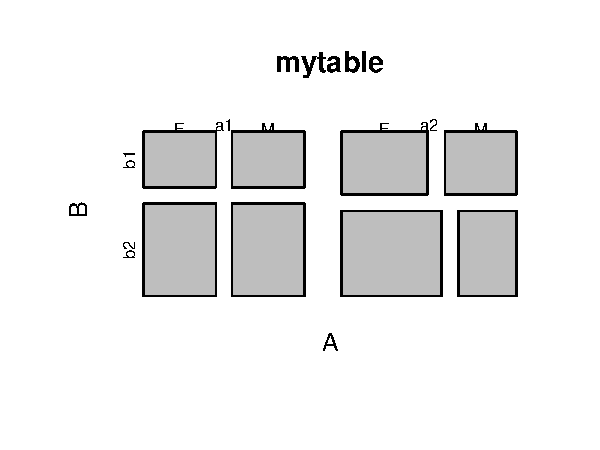
\includegraphics[width=.48\textwidth]{ch02/fig/plot-xtab-1} 
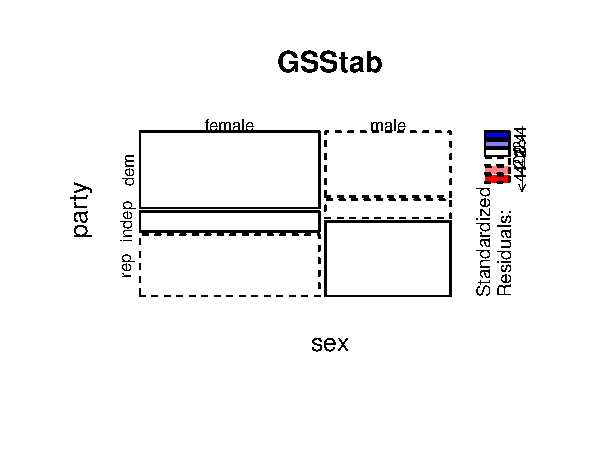
\includegraphics[width=.48\textwidth]{ch02/fig/plot-xtab-2} }

\caption[Mosaic plot of tables using the plot method for table objects]{Mosaic plot of tables using the plot method for table objects\label{fig:plot-xtab}}
\end{figure}


\end{knitrout}



\section[Printing tables: structable and ftable]{Printing tables with \func{structable} and \func{ftable}}\label{sec:structable}

For 3-way and larger tables, the functions
\func{ftable} (in the \pkg{stats} package) and
\func{structable} (in \pkg{vcd}) provide a convenient and flexible tabular display in a ``flat'' (2-way) format.

With \code{ftable(X, row.vars=, col.vars=)}, variables assigned to the rows and/or columns of the result
can be specified as the integer numbers or character names of the variables in
the array \code{X}. By default, the last variable is used for the columns.
The formula method, in the form \verb|ftable(colvars ~ rowvars, data)|
allows a formula, where the left and right hand side of formula specify the column and row variables respectively.

\begin{knitrout}
\definecolor{shadecolor}{rgb}{1, 0.961, 0.933}\color{fgcolor}\begin{kframe}
\begin{alltt}
 \hlkwd{ftable}\hlstd{(UCB)}                    \hlcom{# default}
\end{alltt}
\begin{verbatim}
##                 Department   A   B   C   D   E   F
## Sex    Admitted                                   
## Male   Yes                 512 353 120 138  53  22
##        No                  313 207 205 279 138 351
## Female Yes                  89  17 202 131  94  24
##        No                   19   8 391 244 299 317
\end{verbatim}
\begin{alltt}
\hlcom{#ftable(UCB, row.vars=1:2)      # same result}
 \hlkwd{ftable}\hlstd{(Admitted} \hlopt{+} \hlstd{Sex} \hlopt{~} \hlstd{Department,} \hlkwc{data}\hlstd{=UCB)}   \hlcom{# formula method}
\end{alltt}
\begin{verbatim}
##            Admitted  Yes          No       
##            Sex      Male Female Male Female
## Department                                 
## A                    512     89  313     19
## B                    353     17  207      8
## C                    120    202  205    391
## D                    138    131  279    244
## E                     53     94  138    299
## F                     22     24  351    317
\end{verbatim}
\end{kframe}
\end{knitrout}

The \func{structable} function is similar, but more general, and uses
recursive splits in the vertical or horizontal directions
(similar to the construction of mosaic displays).  It works with both
data frames and table objects.
\begin{knitrout}
\definecolor{shadecolor}{rgb}{1, 0.961, 0.933}\color{fgcolor}\begin{kframe}
\begin{alltt}
\hlkwd{structable}\hlstd{(HairEyeColor)}                   \hlcom{# show the table: default}
\end{alltt}
\begin{verbatim}
##              Eye Brown Blue Hazel Green
## Hair  Sex                              
## Black Male          32   11    10     3
##       Female        36    9     5     2
## Brown Male          53   50    25    15
##       Female        66   34    29    14
## Red   Male          10   10     7     7
##       Female        16    7     7     7
## Blond Male           3   30     5     8
##       Female         4   64     5     8
\end{verbatim}
\begin{alltt}
\hlkwd{structable}\hlstd{(Hair}\hlopt{+}\hlstd{Sex} \hlopt{~} \hlstd{Eye, HairEyeColor)}   \hlcom{# specify col ~ row variables}
\end{alltt}
\begin{verbatim}
##       Hair Black        Brown         Red        Blond       
##       Sex   Male Female  Male Female Male Female  Male Female
## Eye                                                          
## Brown         32     36    53     66   10     16     3      4
## Blue          11      9    50     34   10      7    30     64
## Hazel         10      5    25     29    7      7     5      5
## Green          3      2    15     14    7      7     8      8
\end{verbatim}
\end{kframe}
\end{knitrout}
It also returns an object of class \code{"structable"} for which there are a
variety of special methods.  For example, the transpose function \func{t}
interchanges rows and columns, so that \code{t(structable(HairEyeColor))}
produces the second result shown just above;
\class{structable} objects can be subset using the
\code{[} and \code{[[} operators, using either level indices or names.
There are also plot methods, so that \func{plot} and \func{mosaic}
produce mosaic plots.
\begin{knitrout}
\definecolor{shadecolor}{rgb}{1, 0.961, 0.933}\color{fgcolor}\begin{kframe}
\begin{alltt}
\hlstd{HSE} \hlkwb{<-} \hlkwd{structable}\hlstd{(Hair}\hlopt{+}\hlstd{Sex} \hlopt{~} \hlstd{Eye, HairEyeColor)}   \hlcom{# save structable object}
\hlstd{HSE[}\hlnum{1}\hlopt{:}\hlnum{2}\hlstd{,]}                                         \hlcom{# subset rows}
\end{alltt}
\begin{verbatim}
##       Hair Black        Brown         Red        Blond       
##       Sex   Male Female  Male Female Male Female  Male Female
## Eye                                                          
## Brown         32     36    53     66   10     16     3      4
## Blue          11      9    50     34   10      7    30     64
\end{verbatim}
\begin{alltt}
\hlkwd{mosaic}\hlstd{(HSE,} \hlkwc{shade}\hlstd{=}\hlnum{TRUE}\hlstd{,} \hlkwc{legend}\hlstd{=}\hlnum{FALSE}\hlstd{)}             \hlcom{# plot it}
\end{alltt}
\end{kframe}

\centerline{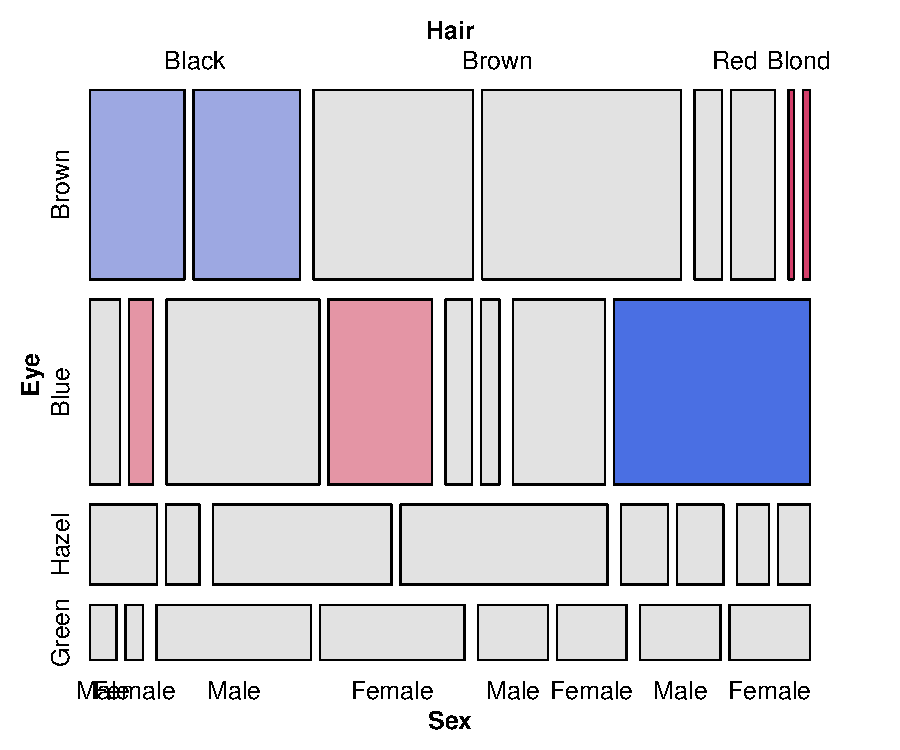
\includegraphics[width=.7\textwidth]{ch02/fig/structable1-1} }



\end{knitrout}

\subsection{Publishing tables to \LaTeX\ or HTML}
OK, you've read your data into \R, done some analysis, and now want to
include some tables in a \LaTeX document or in a web page in HTML format.
Formatting tables for these purposes is often tedious and error-prone.

There are a great many packages in \R that provide for nicely formatted,
publishable tables for a wide variety of purposes; indeed, most of the tables
in this book are generated using these tools.
See \citet{Leifeld:2013:JSS} for description of the \Rpackage{texreg}
and a comparison with some of the other packages.

Here, we simply illustrate the \Rpackage{xtable}, which, along with
capabilities for statistical model summaries, time-series data, and
so forth, has a \code{xtable.table} method for one-way and two-way
table objects.

The \data{HorseKicks} data is a small one-way frequency table
described in \exref{ex:horskick1} and containing the frequencies
of 0, 1, 2, 3, 4 deaths per corps-year by horse-kick among soldiers in 20 corps in
the Prussian army.
\begin{knitrout}
\definecolor{shadecolor}{rgb}{1, 0.961, 0.933}\color{fgcolor}\begin{kframe}
\begin{alltt}
\hlkwd{data}\hlstd{(HorseKicks,} \hlkwc{package}\hlstd{=}\hlstr{"vcd"}\hlstd{)}
\hlstd{HorseKicks}
\end{alltt}
\begin{verbatim}
## nDeaths
##   0   1   2   3   4 
## 109  65  22   3   1
\end{verbatim}
\end{kframe}
\end{knitrout}
By default, \func{xtable} formats this in \LaTeX as a vertical table,
and prints the \LaTeX\ markup to the \R console.  This output is shown
below (without the usual \code{\#\#} comment used to indicate \R output).
\begin{knitrout}
\definecolor{shadecolor}{rgb}{1, 0.961, 0.933}\color{fgcolor}\begin{kframe}
\begin{alltt}
\hlkwd{library}\hlstd{(xtable)}
\hlkwd{xtable}\hlstd{(HorseKicks)}
\end{alltt}
\begin{verbatim}
% latex table generated in R 3.1.1 by xtable 1.7-4 package
% Mon Nov 10 13:27:26 2014
\begin{table}[ht]
\centering
\begin{tabular}{rr}
  \hline
 & nDeaths \\ 
  \hline
0 & 109 \\ 
  1 &  65 \\ 
  2 &  22 \\ 
  3 &   3 \\ 
  4 &   1 \\ 
   \hline
\end{tabular}
\end{table}
\end{verbatim}
\end{kframe}
\end{knitrout}
When this is rendered in a \LaTeX\ document, the result of \func{xtable}
appears as shown in the table below.
\begin{kframe}
\begin{alltt}
\hlkwd{xtable}\hlstd{(HorseKicks)}
\end{alltt}
\end{kframe}% latex table generated in R 3.1.1 by xtable 1.7-4 package
% Mon Nov 10 13:27:26 2014
\begin{table}[ht]
\centering
\begin{tabular}{rr}
  \hline
 & nDeaths \\ 
  \hline
0 & 109 \\ 
  1 &  65 \\ 
  2 &  22 \\ 
  3 &   3 \\ 
  4 &   1 \\ 
   \hline
\end{tabular}
\end{table}


The table above isn't quite right, because the column label ``nDeaths''
belongs to the first column, and the second column should be labeled ``Freq''.
To correct that, we convert the \data{HorseKicks} table to a data frame
(see \secref{sec:convert} for details), add the appropriate \code{colnames},
and use the \code{xtable.print} method to supply some other options.
\begin{kframe}
\begin{alltt}
\hlstd{tab} \hlkwb{<-} \hlkwd{as.data.frame}\hlstd{(HorseKicks)}
\hlkwd{colnames}\hlstd{(tab)} \hlkwb{<-} \hlkwd{c}\hlstd{(}\hlstr{"nDeaths"}\hlstd{,} \hlstr{"Freq"}\hlstd{)}
\hlkwd{print}\hlstd{(}\hlkwd{xtable}\hlstd{(tab),} \hlkwc{include.rownames}\hlstd{=}\hlnum{FALSE}\hlstd{,} \hlkwc{include.colnames}\hlstd{=}\hlnum{TRUE}\hlstd{)}
\end{alltt}
\end{kframe}% latex table generated in R 3.1.1 by xtable 1.7-4 package
% Mon Nov 10 13:27:26 2014
\begin{table}[ht]
\centering
\begin{tabular}{lr}
  \hline
nDeaths & Freq \\ 
  \hline
0 & 109 \\ 
  1 &  65 \\ 
  2 &  22 \\ 
  3 &   3 \\ 
  4 &   1 \\ 
   \hline
\end{tabular}
\end{table}


Finally, in \chref{ch:discrete}, we display a number of similar one-way
frequency tables in a transposed form to save display space.
\tabref{tab:horsetab} is the finished version we show there.
The code below uses the following techniques:
(a) \func{addmargins} is used to show the sum of all the frequency values;
(b) \func{t} transposes the data frame to have 2 rows;
(c) \func{rownames} assigns the labels we want for the rows;
(d) using the \code{caption} argument provides a table caption, and a numbered
table in \LaTeX.
(d) column alignment (\code{"r"} or \code{"l"}) for the table columns
is computed as a character string used for the \code{align} argument.
\begin{kframe}
\begin{alltt}
\hlstd{horsetab} \hlkwb{<-} \hlkwd{t}\hlstd{(} \hlkwd{as.data.frame}\hlstd{(} \hlkwd{addmargins}\hlstd{( HorseKicks ) ) )}
\hlkwd{rownames}\hlstd{( horsetab )} \hlkwb{<-} \hlkwd{c}\hlstd{(} \hlstr{"Number of deaths"}\hlstd{,} \hlstr{"Frequency"} \hlstd{)}
\hlstd{horsetab} \hlkwb{<-} \hlkwd{xtable}\hlstd{( horsetab,} \hlkwc{digits} \hlstd{=} \hlnum{0}\hlstd{,}
     \hlkwc{caption} \hlstd{=} \hlstr{"von Bortkiewicz's data on deaths by horse kicks"}\hlstd{,}
     \hlkwc{align} \hlstd{=} \hlkwd{paste0}\hlstd{(}\hlstr{"l|"}\hlstd{,} \hlkwd{paste}\hlstd{(}\hlkwd{rep}\hlstd{(}\hlstr{"r"}\hlstd{,} \hlkwd{ncol}\hlstd{(horsetab)),} \hlkwc{collapse}\hlstd{=}\hlstr{""}\hlstd{))}
     \hlstd{)}
\hlkwd{print}\hlstd{(horsetab,} \hlkwc{include.colnames}\hlstd{=}\hlnum{FALSE}\hlstd{)}
\end{alltt}
\end{kframe}% latex table generated in R 3.1.1 by xtable 1.7-4 package
% Mon Nov 10 13:27:26 2014
\begin{table}[ht]
\centering
\begin{tabular}{l|rrrrrr}
  \hline
  \hline
Number of deaths & 0 & 1 & 2 & 3 & 4 & Sum \\ 
  Frequency & 109 &  65 &  22 &   3 &   1 & 200 \\ 
   \hline
\end{tabular}
\caption{von Bortkiewicz's data on deaths by horse kicks} 
\end{table}



\section[Collapsing over table factors]{Collapsing over table factors: \func{aggregate}, \func{margin.table} and \func{apply}}\label{sec:collapse}

It sometimes happens that we have a data set with more variables or factors than
we want to analyse, or else, having done some initial analyses, we decide that
certain factors are not important, and so should be excluded from graphic displays
by collapsing (summing) over them.  For example, mosaic plots and fourfold displays
are often simpler to construct from versions of the data collapsed over
the factors which are not shown in the plots.

The appropriate tools to use again depend on
the form in which the data are represented--- a case-form data frame, a
frequency-form data frame (\func{aggregate}), or a table-form array or
table object (\func{margin.table} or \func{apply}).

When the data are in frequency form, and we want to produce another
frequency data frame, \func{aggregate} is a handy tool, using
the argument \code{FUN=sum} to sum the frequency variable over the
factors \emph{not} mentioned in the formula.

\begin{Example}[dayton1]{Dayton survey}
The data frame \data{DaytonSurvey} in the \pkg{vcdExtra} package represents a
$2^5$ table giving the frequencies of reported use (``ever used?'') of
alcohol, cigarettes and marijuana in a sample of 2276 high school seniors,
also classified by sex and race.

\begin{knitrout}
\definecolor{shadecolor}{rgb}{1, 0.961, 0.933}\color{fgcolor}\begin{kframe}
\begin{alltt}
\hlkwd{data}\hlstd{(DaytonSurvey,} \hlkwc{package}\hlstd{=}\hlstr{"vcdExtra"}\hlstd{)}
\hlkwd{str}\hlstd{(DaytonSurvey)}
\end{alltt}
\begin{verbatim}
## 'data.frame':	32 obs. of  6 variables:
##  $ cigarette: Factor w/ 2 levels "Yes","No": 1 2 1 2 1 2 1 2 1 2 ...
##  $ alcohol  : Factor w/ 2 levels "Yes","No": 1 1 2 2 1 1 2 2 1 1 ...
##  $ marijuana: Factor w/ 2 levels "Yes","No": 1 1 1 1 2 2 2 2 1 1 ...
##  $ sex      : Factor w/ 2 levels "female","male": 1 1 1 1 1 1 1 1 2 2 ...
##  $ race     : Factor w/ 2 levels "white","other": 1 1 1 1 1 1 1 1 1 1 ...
##  $ Freq     : num  405 13 1 1 268 218 17 117 453 28 ...
\end{verbatim}
\begin{alltt}
\hlkwd{head}\hlstd{(DaytonSurvey)}
\end{alltt}
\begin{verbatim}
##   cigarette alcohol marijuana    sex  race Freq
## 1       Yes     Yes       Yes female white  405
## 2        No     Yes       Yes female white   13
## 3       Yes      No       Yes female white    1
## 4        No      No       Yes female white    1
## 5       Yes     Yes        No female white  268
## 6        No     Yes        No female white  218
\end{verbatim}
\end{kframe}
\end{knitrout}

To focus on the associations among the
substances, we want to collapse over sex and race. The right-hand side of the formula
used in the call to \func{aggregate} gives the factors to be retained in the
new frequency data frame, \code{Dayton.ACM.df}.  The left-hand side is
the frequency variable (\code{Freq}), and we aggregate using the \code{FUN=sum}.

\begin{knitrout}
\definecolor{shadecolor}{rgb}{1, 0.961, 0.933}\color{fgcolor}\begin{kframe}
\begin{alltt}
\hlcom{# data in frequency form: collapse over sex and race}
\hlstd{Dayton.ACM.df} \hlkwb{<-} \hlkwd{aggregate}\hlstd{(Freq} \hlopt{~} \hlstd{cigarette}\hlopt{+}\hlstd{alcohol}\hlopt{+}\hlstd{marijuana,}
                           \hlkwc{data}\hlstd{=DaytonSurvey,} \hlkwc{FUN}\hlstd{=sum)}
\hlstd{Dayton.ACM.df}
\end{alltt}
\begin{verbatim}
##   cigarette alcohol marijuana Freq
## 1       Yes     Yes       Yes  911
## 2        No     Yes       Yes   44
## 3       Yes      No       Yes    3
## 4        No      No       Yes    2
## 5       Yes     Yes        No  538
## 6        No     Yes        No  456
## 7       Yes      No        No   43
## 8        No      No        No  279
\end{verbatim}
\end{kframe}
\end{knitrout}
\end{Example}

When the data are in table form, and we want to produce another
table, \func{apply} with \code{FUN=sum} can be used in a similar way
to sum the table over dimensions not mentioned in the \code{MARGIN}
argument.  \func{margin.table} is just a wrapper for \func{apply}
using the \func{sum} function.


\begin{Example}[dayton2]{Dayton survey}
To illustrate, we first convert the \data{DaytonSurvey} to a 5-way
table using \func{xtabs}, giving \code{Dayton.tab}.

\begin{knitrout}
\definecolor{shadecolor}{rgb}{1, 0.961, 0.933}\color{fgcolor}\begin{kframe}
\begin{alltt}
\hlcom{# convert to table form}
\hlstd{Dayton.tab} \hlkwb{<-} \hlkwd{xtabs}\hlstd{(Freq}\hlopt{~}\hlstd{cigarette}\hlopt{+}\hlstd{alcohol}\hlopt{+}\hlstd{marijuana}\hlopt{+}\hlstd{sex}\hlopt{+}\hlstd{race,}
                    \hlkwc{data}\hlstd{=DaytonSurvey)}
\hlkwd{structable}\hlstd{(cigarette}\hlopt{+}\hlstd{alcohol}\hlopt{+}\hlstd{marijuana} \hlopt{~} \hlstd{sex}\hlopt{+}\hlstd{race,} \hlkwc{data}\hlstd{=Dayton.tab)}
\end{alltt}
\begin{verbatim}
##              cigarette Yes              No            
##              alcohol   Yes      No     Yes      No    
##              marijuana Yes  No Yes  No Yes  No Yes  No
## sex    race                                           
## female white           405 268   1  17  13 218   1 117
##        other            23  23   0   1   2  19   0  12
## male   white           453 228   1  17  28 201   1 133
##        other            30  19   1   8   1  18   0  17
\end{verbatim}
\end{kframe}
\end{knitrout}
Then, use \func{apply} on \code{Dayton.tab} to give the
3-way table \code{Dayton.ACM.tab} summed over sex and race.
The elements in this new table are the column sums for
\code{Dayton.tab} shown by \func{structable} just above.

\begin{knitrout}
\definecolor{shadecolor}{rgb}{1, 0.961, 0.933}\color{fgcolor}\begin{kframe}
\begin{alltt}
\hlcom{# collapse over sex and race}
\hlstd{Dayton.ACM.tab} \hlkwb{<-} \hlkwd{apply}\hlstd{(Dayton.tab,} \hlkwc{MARGIN}\hlstd{=}\hlnum{1}\hlopt{:}\hlnum{3}\hlstd{,} \hlkwc{FUN}\hlstd{=sum)}
\hlstd{Dayton.ACM.tab} \hlkwb{<-} \hlkwd{margin.table}\hlstd{(Dayton.tab,} \hlnum{1}\hlopt{:}\hlnum{3}\hlstd{)}   \hlcom{# same result}
\hlkwd{structable}\hlstd{(cigarette}\hlopt{+}\hlstd{alcohol} \hlopt{~} \hlstd{marijuana,} \hlkwc{data}\hlstd{=Dayton.ACM.tab)}
\end{alltt}
\begin{verbatim}
##           cigarette Yes      No    
##           alcohol   Yes  No Yes  No
## marijuana                          
## Yes                 911   3  44   2
## No                  538  43 456 279
\end{verbatim}
\end{kframe}
\end{knitrout}
\end{Example}

Many of these operations can be performed using the \verb|**ply()| functions
in the \pkg{plyr} package.
For example, with the data in a frequency form data frame, use \func{ddply}
to collapse over unmentioned factors, and \func{plyr::summarise}%
\footnote{
Ugh. This \pkg{plyr} function clashes with a function of the same name in \pkg{vcdExtra}.
In this book I will use the explicit double-colon notation to keep them
separate.
}
as the function to be applied to each piece.
\begin{knitrout}
\definecolor{shadecolor}{rgb}{1, 0.961, 0.933}\color{fgcolor}\begin{kframe}
\begin{alltt}
\hlstd{Dayton.ACM.df} \hlkwb{<-} \hlkwd{ddply}\hlstd{(DaytonSurvey,} \hlkwd{.}\hlstd{(cigarette, alcohol, marijuana),}
                       \hlstd{plyr}\hlopt{::}\hlstd{summarise,} \hlkwc{Freq}\hlstd{=}\hlkwd{sum}\hlstd{(Freq))}
\end{alltt}
\end{kframe}
\end{knitrout}

\subsection[Collapsing table levels]{Collapsing table levels: \func{collapse.table}}

A related problem arises when we have a table or array and for some purpose
we want to reduce the number of levels of some factors by summing subsets
of the frequencies.  For example, we may have initially coded Age in 10-year
intervals, and decide that, either for analysis or display purposes, we
want to reduce Age to 20-year intervals.  The \func{collapse.table} function
in \pkg{vcdExtra} was designed for this purpose.

\begin{Example}[collapse-cat]{Collapsing categories}
Create a 3-way table, and collapse Age from 10-year to 20-year intervals
and Education from three levels to two.
To illustrate, we first generate a $2 \times 6 \times 3$ table of random counts from a
Poisson distribution with mean of 100, with factors \var{sex}, \var{age}
and \var{education}.
\begin{knitrout}
\definecolor{shadecolor}{rgb}{1, 0.961, 0.933}\color{fgcolor}\begin{kframe}
\begin{alltt}
\hlcom{# create some sample data in frequency form}
\hlstd{sex} \hlkwb{<-} \hlkwd{c}\hlstd{(}\hlstr{"Male"}\hlstd{,} \hlstr{"Female"}\hlstd{)}
\hlstd{age} \hlkwb{<-} \hlkwd{c}\hlstd{(}\hlstr{"10-19"}\hlstd{,} \hlstr{"20-29"}\hlstd{,}  \hlstr{"30-39"}\hlstd{,} \hlstr{"40-49"}\hlstd{,} \hlstr{"50-59"}\hlstd{,} \hlstr{"60-69"}\hlstd{)}
\hlstd{education} \hlkwb{<-} \hlkwd{c}\hlstd{(}\hlstr{"low"}\hlstd{,} \hlstr{'med'}\hlstd{,} \hlstr{'high'}\hlstd{)}
\hlstd{dat} \hlkwb{<-} \hlkwd{expand.grid}\hlstd{(}\hlkwc{sex}\hlstd{=sex,} \hlkwc{age}\hlstd{=age,} \hlkwc{education}\hlstd{=education)}
\hlstd{counts} \hlkwb{<-} \hlkwd{rpois}\hlstd{(}\hlnum{36}\hlstd{,} \hlnum{100}\hlstd{)}   \hlcom{# random Poisson cell frequencies}
\hlstd{dat} \hlkwb{<-} \hlkwd{cbind}\hlstd{(dat, counts)}
\hlcom{# make it into a 3-way table}
\hlstd{tab1} \hlkwb{<-} \hlkwd{xtabs}\hlstd{(counts} \hlopt{~} \hlstd{sex} \hlopt{+} \hlstd{age} \hlopt{+} \hlstd{education,} \hlkwc{data}\hlstd{=dat)}
\hlkwd{structable}\hlstd{(tab1)}
\end{alltt}
\begin{verbatim}
##                  age 10-19 20-29 30-39 40-49 50-59 60-69
## sex    education                                        
## Male   low              91   110   106    95   107    98
##        med             108   104    97   100   107   112
##        high            104   104   106   101    92    95
## Female low             115   103    96    93   112    94
##        med              96    88    92   103    98    93
##        high             84    93   103    93    95   103
\end{verbatim}
\end{kframe}
\end{knitrout}
Now collapse \code{age} to 20-year intervals, and \code{education}
to 2 levels. In the arguments to \func{collapse.table}, levels of \code{age} and \code{education}
given the same label are summed in the resulting smaller table.
\begin{knitrout}
\definecolor{shadecolor}{rgb}{1, 0.961, 0.933}\color{fgcolor}\begin{kframe}
\begin{alltt}
\hlcom{# collapse age to 3 levels, education to 2 levels}
\hlstd{tab2} \hlkwb{<-} \hlkwd{collapse.table}\hlstd{(tab1,}
         \hlkwc{age}\hlstd{=}\hlkwd{c}\hlstd{(}\hlstr{"10-29"}\hlstd{,} \hlstr{"10-29"}\hlstd{,}  \hlstr{"30-49"}\hlstd{,} \hlstr{"30-49"}\hlstd{,} \hlstr{"50-69"}\hlstd{,} \hlstr{"50-69"}\hlstd{),}
         \hlkwc{education}\hlstd{=}\hlkwd{c}\hlstd{(}\hlstr{"<high"}\hlstd{,} \hlstr{"<high"}\hlstd{,} \hlstr{"high"}\hlstd{))}
\hlkwd{structable}\hlstd{(tab2)}
\end{alltt}
\begin{verbatim}
##                  age 10-29 30-49 50-69
## sex    education                      
## Male   <high           413   398   424
##        high            208   207   187
## Female <high           402   384   397
##        high            177   196   198
\end{verbatim}
\end{kframe}
\end{knitrout}
\end{Example}

\section{Converting among frequency tables and data frames}\label{sec:convert}

As we've seen, a given contingency table can be represented
equivalently in case form, frequency form and table form.
However, some \R functions were designed for one particular representation.
\tabref{tab:convert} shows some handy tools for converting from one form to another.

\begin{table}[htb]
 \caption{Tools for converting among different forms for categorical data}\label{tab:convert}
 \newsavebox{\adfxtabs}
 \savebox{\adfxtabs}{\begin{tabular}{ll} \code{Z <- xtabs(~A+B)} \\ \code{as.data.frame(Z)} \\ \end{tabular}}
 \begin{center}
   \begin{tabular}{l|lll}
  \hline
                 & \multicolumn{3}{c}{\textbf{To this}} \\
	\textbf{From this}      &     Case form         & Frequency form             &  Table form \\
	\hline
  Case form      &                        & \usebox{\adfxtabs}        &  \verb|table(A,B)|  \\
%	Case form      &                        & {\small\verb|as.data.frame(xtabs(~A+B))|}        &  \verb|table(A,B)|  \\
	Frequency form &  \verb|expand.dft(X)|  &                           & \verb|xtabs(count~A+B)|\\
	Table form     &  \verb|expand.dft(X)|  & \verb|as.data.frame(X)|   &       \\
	\hline
   \end{tabular}
 \end{center}
\end{table}

\subsection{Table form to frequency form}
A contingency table in table form (an object of class \class{table}) can be converted
to a data frame in frequency form with \func{as.data.frame}.%
\footnote{
Because \R is object-oriented, this is actually a short-hand for
the function \func{as.data.frame.table}.
}
The resulting
data frame contains columns
representing the classifying factors and the table entries (as a column named by
the \code{responseName} argument, defaulting to \code{Freq}.  The function
\func{as.data.frame} is the inverse of \func{xtabs}, which converts a data frame to a table.

\begin{Example}[GSS-convert]{General social survey}
Convert the \code{GSStab} in table form to a data.frame in frequency form.
By default, the frequency variable is named \code{Freq}, and the variables
\code{sex} and \code{party} are made factors.
\begin{knitrout}
\definecolor{shadecolor}{rgb}{1, 0.961, 0.933}\color{fgcolor}\begin{kframe}
\begin{alltt}
\hlkwd{as.data.frame}\hlstd{(GSStab)}
\end{alltt}
\begin{verbatim}
##      sex party Freq
## 1 female   dem  279
## 2   male   dem  165
## 3 female indep   73
## 4   male indep   47
## 5 female   rep  225
## 6   male   rep  191
\end{verbatim}
\end{kframe}
\end{knitrout}
\end{Example}

In addition, there are situations where numeric table variables are represented as
factors, but you need to
convert them to numerics for calculation purposes.

\begin{Example}[horse.df]{Death by horse kick}

For example, We might want to calculate the weighted mean of \code{nDeaths}
in the \data{HorseKicks} data.
Using \func{as.data.frame} won't work here, because the variable \code{nDeaths}
becomes a factor.

\begin{knitrout}
\definecolor{shadecolor}{rgb}{1, 0.961, 0.933}\color{fgcolor}\begin{kframe}
\begin{alltt}
\hlkwd{str}\hlstd{(}\hlkwd{as.data.frame}\hlstd{(HorseKicks))}
\end{alltt}
\begin{verbatim}
## 'data.frame':	5 obs. of  2 variables:
##  $ nDeaths: Factor w/ 5 levels "0","1","2","3",..: 1 2 3 4 5
##  $ Freq   : int  109 65 22 3 1
\end{verbatim}
\end{kframe}
\end{knitrout}
One solution is to use \func{data.frame} directly and \func{as.numeric}
to coerce the table names to numbers.
\begin{knitrout}
\definecolor{shadecolor}{rgb}{1, 0.961, 0.933}\color{fgcolor}\begin{kframe}
\begin{alltt}
\hlstd{horse.df} \hlkwb{<-} \hlkwd{data.frame}\hlstd{(}\hlkwc{nDeaths} \hlstd{=} \hlkwd{as.numeric}\hlstd{(}\hlkwd{names}\hlstd{(HorseKicks)),}
                       \hlkwc{Freq} \hlstd{=} \hlkwd{as.vector}\hlstd{(HorseKicks))}
\hlkwd{str}\hlstd{(horse.df)}
\end{alltt}
\begin{verbatim}
## 'data.frame':	5 obs. of  2 variables:
##  $ nDeaths: num  0 1 2 3 4
##  $ Freq   : int  109 65 22 3 1
\end{verbatim}
\begin{alltt}
\hlstd{horse.df}
\end{alltt}
\begin{verbatim}
##   nDeaths Freq
## 1       0  109
## 2       1   65
## 3       2   22
## 4       3    3
## 5       4    1
\end{verbatim}
\end{kframe}
\end{knitrout}
Then, \func{weighted.mean} works as we would like:
\begin{knitrout}
\definecolor{shadecolor}{rgb}{1, 0.961, 0.933}\color{fgcolor}\begin{kframe}
\begin{alltt}
\hlkwd{weighted.mean}\hlstd{(horse.df}\hlopt{$}\hlstd{nDeaths,} \hlkwc{weights}\hlstd{=horse.df}\hlopt{$}\hlstd{Freq)}
\end{alltt}
\begin{verbatim}
## [1] 2
\end{verbatim}
\end{kframe}
\end{knitrout}
\end{Example}

\subsection{Case form to table form}
Going the other way, we use \func{table} to convert from case form to table form.

\begin{Example}[Arth-convert]{Arthritis treatment}
Convert the \code{Arthritis} data in case form to a 3-way table of
\code{Treatment} $\times$ \code{Sex} $\times$ \code{Improved}.
We select the desired columns with their names, but could also use column
numbers, e.g., \code{table(Arthritis[,c(2,3,5)])}.
%Note the use of \func{with} to avoid having to use \code{Arthritis\$Treatment} etc. within %the call to \func{table}.%
\begin{knitrout}
\definecolor{shadecolor}{rgb}{1, 0.961, 0.933}\color{fgcolor}\begin{kframe}
\begin{alltt}
\hlstd{Art.tab} \hlkwb{<-} \hlkwd{table}\hlstd{(Arthritis[,}\hlkwd{c}\hlstd{(}\hlstr{"Treatment"}\hlstd{,} \hlstr{"Sex"}\hlstd{,} \hlstr{"Improved"}\hlstd{)])}
\hlkwd{str}\hlstd{(Art.tab)}
\end{alltt}
\begin{verbatim}
##  'table' int [1:2, 1:2, 1:3] 19 6 10 7 7 5 0 2 6 16 ...
##  - attr(*, "dimnames")=List of 3
##   ..$ Treatment: chr [1:2] "Placebo" "Treated"
##   ..$ Sex      : chr [1:2] "Female" "Male"
##   ..$ Improved : chr [1:3] "None" "Some" "Marked"
\end{verbatim}
\begin{alltt}
\hlkwd{ftable}\hlstd{(Art.tab)}
\end{alltt}
\begin{verbatim}
##                  Improved None Some Marked
## Treatment Sex                             
## Placebo   Female            19    7      6
##           Male              10    0      1
## Treated   Female             6    5     16
##           Male               7    2      5
\end{verbatim}
\end{kframe}
\end{knitrout}
\end{Example}

\subsection{Table form to case form}
There may also be times that you will need an equivalent case form data frame
with factors  representing the table variables
rather than the frequency  table.
For example, the \func{mca} function in package \pkg{MASS}
only operates on data in this format.
The function \func{expand.dft}%
\footnote{
The original code for this function was provided by Marc Schwarz on the R-Help
mailing list.
}
in \pkg{vcdExtra}
does this, converting a table into a case form.

\begin{Example}[Arth-convert2]{Arthritis treatment}
Convert the \data{Arthritis} data in table form (\code{Art.tab}) back to a \code{data.frame}
in case form, with factors
\code{Treatment}, \code{Sex} and \code{Improved}.
\begin{knitrout}\footnotesize
\definecolor{shadecolor}{rgb}{1, 0.961, 0.933}\color{fgcolor}\begin{kframe}
\begin{alltt}
\hlstd{Art.df} \hlkwb{<-} \hlkwd{expand.dft}\hlstd{(Art.tab)}
\hlkwd{str}\hlstd{(Art.df)}
\end{alltt}
\begin{verbatim}
## 'data.frame':	84 obs. of  3 variables:
##  $ Treatment: Factor w/ 2 levels "Placebo","Treated": 1 1 1 1 1 1 1 1 1 1 ...
##  $ Sex      : Factor w/ 2 levels "Female","Male": 1 1 1 1 1 1 1 1 1 1 ...
##  $ Improved : Factor w/ 3 levels "Marked","None",..: 2 2 2 2 2 2 2 2 2 2 ...
\end{verbatim}
\end{kframe}
\end{knitrout}
\end{Example}


\section{A complex example: TV viewing data}\label{sec:working-complex}

If you've followed so far, congratulations! You're ready for a more complicated example
that puts together a variety of the skills developed in this chapter:
\begin{seriate}
  \item reading raw data,
  \item creating tables,
  \item assigning level names to factors and
  \item collapsing levels or variables for use in analysis.
\end{seriate}

\ixeon{TV viewing data}
For illustration of these steps,
we use the dataset \code{tv.dat}, supplied with
the initial implementation of
mosaic displays in \R by Jay Emerson.
In turn, they were derived from an early, compelling example of mosaic displays
\citep{HartiganKleiner:84},
that illustrated the method with data on a large sample of TV viewers
whose behavior had been recorded for the Neilsen ratings.
This data set contains sample television audience data from Neilsen
Media Research for the week starting November 6, 1995.


The data file, \code{tv.dat} is stored in frequency form
as a file with 825 rows and 5 columns.  There is no header line
in the file, so when we use \func{read.table} below, the variables
will be named \code{V1} -- \code{V5}.  This data represents
 a 4-way table of size
$5 \times 11 \times 5 \times 3 = 825$ where the table variables
are \code{V1} -- \code{V4}, and the cell frequency is read
as \code{V5}.

%% should use \begin{description} ... here
\begin{flushleft}
The table variables are:\\
~~~\code{V1}-- values 1:5 correspond to the days Monday--Friday;\\
~~~\code{V2}-- values 1:11 correspond to the quarter hour times 8:00PM through 10:30PM;\\
~~~\code{V3}-- values 1:5 correspond to ABC, CBS, NBC, Fox, and non-network choices;\\
~~~\code{V4}-- values 1:3 correspond to transition states: turn the television Off, Switch channels,  or Persist in viewing the current channel.
\end{flushleft}

\subsection{Creating data frames and arrays}
The file \code{tv.dat} is stored in the \code{doc/extdata} directory
of \pkg{vcdExtra}; it can be read as follows:
\begin{knitrout}
\definecolor{shadecolor}{rgb}{1, 0.961, 0.933}\color{fgcolor}\begin{kframe}
\begin{alltt}
\hlstd{tv.data}\hlkwb{<-}\hlkwd{read.table}\hlstd{(}\hlkwd{system.file}\hlstd{(}\hlstr{"doc"}\hlstd{,}\hlstr{"extdata"}\hlstd{,}\hlstr{"tv.dat"}\hlstd{,}\hlkwc{package}\hlstd{=}\hlstr{"vcdExtra"}\hlstd{))}
\hlkwd{str}\hlstd{(tv.data)}
\end{alltt}
\begin{verbatim}
## 'data.frame':	825 obs. of  5 variables:
##  $ V1: int  1 2 3 4 5 1 2 3 4 5 ...
##  $ V2: int  1 1 1 1 1 2 2 2 2 2 ...
##  $ V3: int  1 1 1 1 1 1 1 1 1 1 ...
##  $ V4: int  1 1 1 1 1 1 1 1 1 1 ...
##  $ V5: int  6 18 6 2 11 6 29 25 17 29 ...
\end{verbatim}
\begin{alltt}
\hlkwd{head}\hlstd{(tv.data,}\hlnum{5}\hlstd{)}
\end{alltt}
\begin{verbatim}
##   V1 V2 V3 V4 V5
## 1  1  1  1  1  6
## 2  2  1  1  1 18
## 3  3  1  1  1  6
## 4  4  1  1  1  2
## 5  5  1  1  1 11
\end{verbatim}
\end{kframe}
\end{knitrout}
To read such data from a local file, just use \func{read.table} in this form:
\begin{knitrout}
\definecolor{shadecolor}{rgb}{1, 0.961, 0.933}\color{fgcolor}\begin{kframe}
\begin{alltt}
\hlstd{tv.data}\hlkwb{<-}\hlkwd{read.table}\hlstd{(}\hlstr{"C:/R/data/tv.dat"}\hlstd{)}
\end{alltt}
\end{kframe}
\end{knitrout}

We could use this data in frequency form for analysis by renaming the variables,
and converting the integer-coded factors \code{V1} -- \code{V4} to \R factors.
The lines below use the function \func{within} to avoid having to use
\verb|TV.dat$Day <- factor(TV.dat$Day)| etc., and only supplies labels for the
first variable.
\begin{knitrout}\footnotesize
\definecolor{shadecolor}{rgb}{1, 0.961, 0.933}\color{fgcolor}\begin{kframe}
\begin{alltt}
\hlstd{TV.df} \hlkwb{<-} \hlstd{tv.data}
\hlkwd{colnames}\hlstd{(TV.df)} \hlkwb{<-} \hlkwd{c}\hlstd{(}\hlstr{"Day"}\hlstd{,} \hlstr{"Time"}\hlstd{,} \hlstr{"Network"}\hlstd{,} \hlstr{"State"}\hlstd{,} \hlstr{"Freq"}\hlstd{)}
\hlstd{TV.df} \hlkwb{<-} \hlkwd{within}\hlstd{(TV.df, \{Day} \hlkwb{<-} \hlkwd{factor}\hlstd{(Day,}
                                      \hlkwc{labels}\hlstd{=}\hlkwd{c}\hlstd{(}\hlstr{"Mon"}\hlstd{,} \hlstr{"Tue"}\hlstd{,} \hlstr{"Wed"}\hlstd{,} \hlstr{"Thu"}\hlstd{,} \hlstr{"Fri"}\hlstd{))}
                        \hlstd{Time} \hlkwb{<-} \hlkwd{factor}\hlstd{(Time)}
                        \hlstd{Network} \hlkwb{<-} \hlkwd{factor}\hlstd{(Network)}
                        \hlstd{State} \hlkwb{<-} \hlkwd{factor}\hlstd{(State)\})}
\end{alltt}
\end{kframe}
\end{knitrout}

Alternatively, we could just reshape the frequency column
(\code{V5} or \code{tv.data[,5]}) into
a 4-way array.
In the lines below, we rely on the facts that the
(a) the table is complete--- there are no missing cells,
so \code{nrow(tv.data)}=825;
(b) the observations are ordered so that \code{V1} varies most rapidly and
\code{V4} most slowly.  From this, we can just extract the frequency column
and reshape it into an array using the \code{dim} argument.
The level names are assigned to \code{dimnames(TV)}
and the variable names to \code{names(dimnames(TV))}.
\begin{knitrout}
\definecolor{shadecolor}{rgb}{1, 0.961, 0.933}\color{fgcolor}\begin{kframe}
\begin{alltt}
\hlstd{TV} \hlkwb{<-} \hlkwd{array}\hlstd{(tv.data[,}\hlnum{5}\hlstd{],} \hlkwc{dim}\hlstd{=}\hlkwd{c}\hlstd{(}\hlnum{5}\hlstd{,}\hlnum{11}\hlstd{,}\hlnum{5}\hlstd{,}\hlnum{3}\hlstd{))}
\hlkwd{dimnames}\hlstd{(TV)} \hlkwb{<-} \hlkwd{list}\hlstd{(}\hlkwd{c}\hlstd{(}\hlstr{"Mon"}\hlstd{,}\hlstr{"Tue"}\hlstd{,}\hlstr{"Wed"}\hlstd{,}\hlstr{"Thu"}\hlstd{,}\hlstr{"Fri"}\hlstd{),}
                \hlkwd{c}\hlstd{(}\hlstr{"8:00"}\hlstd{,}\hlstr{"8:15"}\hlstd{,}\hlstr{"8:30"}\hlstd{,}\hlstr{"8:45"}\hlstd{,}\hlstr{"9:00"}\hlstd{,}\hlstr{"9:15"}\hlstd{,}\hlstr{"9:30"}\hlstd{,}
                  \hlstr{"9:45"}\hlstd{,}\hlstr{"10:00"}\hlstd{,}\hlstr{"10:15"}\hlstd{,}\hlstr{"10:30"}\hlstd{),}
                \hlkwd{c}\hlstd{(}\hlstr{"ABC"}\hlstd{,}\hlstr{"CBS"}\hlstd{,}\hlstr{"NBC"}\hlstd{,}\hlstr{"Fox"}\hlstd{,}\hlstr{"Other"}\hlstd{),}
                \hlkwd{c}\hlstd{(}\hlstr{"Off"}\hlstd{,}\hlstr{"Switch"}\hlstd{,}\hlstr{"Persist"}\hlstd{))}
\hlkwd{names}\hlstd{(}\hlkwd{dimnames}\hlstd{(TV))}\hlkwb{<-}\hlkwd{c}\hlstd{(}\hlstr{"Day"}\hlstd{,} \hlstr{"Time"}\hlstd{,} \hlstr{"Network"}\hlstd{,} \hlstr{"State"}\hlstd{)}
\end{alltt}
\end{kframe}
\end{knitrout}

More generally (even if there are missing cells), we can
use \func{xtabs} (or \func{plyr::daply})
to do the cross-tabulation, using \code{V5} as the
frequency variable.  Here's how to do this same operation with \func{xtabs}:
\begin{knitrout}
\definecolor{shadecolor}{rgb}{1, 0.961, 0.933}\color{fgcolor}\begin{kframe}
\begin{alltt}
\hlstd{TV} \hlkwb{<-} \hlkwd{xtabs}\hlstd{(V5} \hlopt{~} \hlstd{.,} \hlkwc{data}\hlstd{=tv.data)}
\hlkwd{dimnames}\hlstd{(TV)} \hlkwb{<-} \hlkwd{list}\hlstd{(}\hlkwc{Day}\hlstd{=}\hlkwd{c}\hlstd{(}\hlstr{"Mon"}\hlstd{,}\hlstr{"Tue"}\hlstd{,}\hlstr{"Wed"}\hlstd{,}\hlstr{"Thu"}\hlstd{,}\hlstr{"Fri"}\hlstd{),}
                \hlkwc{Time}\hlstd{=}\hlkwd{c}\hlstd{(}\hlstr{"8:00"}\hlstd{,}\hlstr{"8:15"}\hlstd{,}\hlstr{"8:30"}\hlstd{,}\hlstr{"8:45"}\hlstd{,}\hlstr{"9:00"}\hlstd{,}\hlstr{"9:15"}\hlstd{,}\hlstr{"9:30"}\hlstd{,}
                       \hlstr{"9:45"}\hlstd{,}\hlstr{"10:00"}\hlstd{,}\hlstr{"10:15"}\hlstd{,}\hlstr{"10:30"}\hlstd{),}
                \hlkwc{Network}\hlstd{=}\hlkwd{c}\hlstd{(}\hlstr{"ABC"}\hlstd{,}\hlstr{"CBS"}\hlstd{,}\hlstr{"NBC"}\hlstd{,}\hlstr{"Fox"}\hlstd{,}\hlstr{"Other"}\hlstd{),}
                \hlkwc{State}\hlstd{=}\hlkwd{c}\hlstd{(}\hlstr{"Off"}\hlstd{,}\hlstr{"Switch"}\hlstd{,}\hlstr{"Persist"}\hlstd{))}
\end{alltt}
\end{kframe}
\end{knitrout}
\noindent Note that in the lines above, the variable names are assigned directly
as the names of the elements in the \code{dimnames} list.

\subsection{Subsetting and collapsing}
For many purposes,
the 4-way table \code{TV}
is too large and awkward to work with. Among the networks,
Fox and Other occur infrequently, so we will remove them.
We can also cut it down to a 3-way table by considering only viewers who persist
with the current station.%
\footnote{This relies on the fact that indexing
an array drops dimensions of length 1 by default,
using the argument \code{drop=TRUE};
the result is coerced to the lowest possible dimension.
}

\begin{knitrout}\footnotesize
\definecolor{shadecolor}{rgb}{1, 0.961, 0.933}\color{fgcolor}\begin{kframe}
\begin{alltt}
\hlstd{TV} \hlkwb{<-} \hlstd{TV[,,}\hlnum{1}\hlopt{:}\hlnum{3}\hlstd{,]}     \hlcom{# keep only ABC, CBS, NBC}
\hlstd{TV} \hlkwb{<-} \hlstd{TV[,,,}\hlnum{3}\hlstd{]}       \hlcom{# keep only Persist -- now a 3 way table}
\hlkwd{structable}\hlstd{(TV)}
\end{alltt}
\begin{verbatim}
##             Time 8:00 8:15 8:30 8:45 9:00 9:15 9:30 9:45 10:00 10:15 10:30
## Day Network                                                               
## Mon ABC           146  151  156   83  325  350  386  340   352   280   278
##     CBS           337  293  304  233  311  251  241  164   252   265   272
##     NBC           263  219  236  140  226  235  239  246   279   263   283
## Tue ABC           244  181  231  205  385  283  345  192   329   351   364
##     CBS           173  180  184  109  218  235  256  250   274   263   261
##     NBC           315  254  280  241  370  214  195  111   188   190   210
## Wed ABC           233  161  194  156  339  264  279  140   237   228   203
##     CBS           158  126  207   59   98  103  122   86   109   105   110
##     NBC           134  146  166   66  194  230  264  143   274   289   306
## Thu ABC           174  183  197  181  187  198  211   86   110   122   117
##     CBS           196  185  195  104  106  116  116   47   102    84    84
##     NBC           515  463  472  477  590  473  446  349   649   705   747
## Fri ABC           294  281  305  239  278  246  245  138   246   232   233
##     CBS           130  144  154   81  129  153  136  126   138   136   152
##     NBC           195  220  248  160  172  164  169   85   183   198   204
\end{verbatim}
\end{kframe}
\end{knitrout}

Finally, for some purposes, we might also want to collapse the 11 times into a smaller number.
Here, we use \func{as.data.frame.table} to convert the table back to a data frame,
 \func{levels} to re-assign the values of \code{Time},
 and finally, \func{xtabs} to give a new, collapsed frequency table.

\begin{knitrout}
\definecolor{shadecolor}{rgb}{1, 0.961, 0.933}\color{fgcolor}\begin{kframe}
\begin{alltt}
\hlstd{TV.df} \hlkwb{<-} \hlkwd{as.data.frame.table}\hlstd{(TV)}
\hlkwd{levels}\hlstd{(TV.df}\hlopt{$}\hlstd{Time)} \hlkwb{<-} \hlkwd{c}\hlstd{(}\hlkwd{rep}\hlstd{(}\hlstr{"8:00-8:59"}\hlstd{,}\hlnum{4}\hlstd{),}
                        \hlkwd{rep}\hlstd{(}\hlstr{"9:00-9:59"}\hlstd{,}\hlnum{4}\hlstd{),} \hlkwd{rep}\hlstd{(}\hlstr{"10:00-10:44"}\hlstd{,}\hlnum{3}\hlstd{))}
\hlstd{TV2} \hlkwb{<-} \hlkwd{xtabs}\hlstd{(Freq} \hlopt{~} \hlstd{Day} \hlopt{+} \hlstd{Time} \hlopt{+} \hlstd{Network, TV.df)}
\hlkwd{structable}\hlstd{(Day} \hlopt{~} \hlstd{Time}\hlopt{+}\hlstd{Network,TV2)}
\end{alltt}
\begin{verbatim}
##                     Day  Mon  Tue  Wed  Thu  Fri
## Time        Network                             
## 8:00-8:59   ABC          536  861  744  735 1119
##             CBS         1167  646  550  680  509
##             NBC          858 1090  512 1927  823
## 9:00-9:59   ABC         1401 1205 1022  682  907
##             CBS          967  959  409  385  544
##             NBC          946  890  831 1858  590
## 10:00-10:44 ABC          910 1044  668  349  711
##             CBS          789  798  324  270  426
##             NBC          825  588  869 2101  585
\end{verbatim}
\end{kframe}
\end{knitrout}
Congratulations! If you followed the operations described above,
you are ready for the material described in the rest of the book.
If not, try working through some of exercises below.

As a final step and a prelude to what follows, we construct a mosaic
plot, below (\figref{fig:TV-mosaic}) that focuses on the associations
between the combinations of \code{Day} and \code{Time} and the
\code{Network} viewed.  In terms of a \loglin model, this is
represented by the model formula \verb|~Day:Time + Network|,
which asserts that \code{Network} is independent of the
\code{Day:Time} combinations.

\begin{knitrout}
\definecolor{shadecolor}{rgb}{1, 0.961, 0.933}\color{fgcolor}\begin{kframe}
\begin{alltt}
\hlkwd{dimnames}\hlstd{(TV2)}\hlopt{$}\hlstd{Time} \hlkwb{<-} \hlkwd{c}\hlstd{(}\hlstr{"8"}\hlstd{,} \hlstr{"9"}\hlstd{,} \hlstr{"10"}\hlstd{)}     \hlcom{# re-level for mosaic display}
\hlkwd{mosaic}\hlstd{(}\hlopt{~} \hlstd{Day} \hlopt{+} \hlstd{Network} \hlopt{+} \hlstd{Time,} \hlkwc{data}\hlstd{=TV2,} \hlkwc{expected}\hlstd{=}\hlopt{~}\hlstd{Day}\hlopt{:}\hlstd{Time} \hlopt{+} \hlstd{Network,}
         \hlkwc{legend}\hlstd{=}\hlnum{FALSE}\hlstd{,} \hlkwc{gp}\hlstd{=shading_Friendly)}
\end{alltt}
\end{kframe}\begin{figure}[!htb]


\centerline{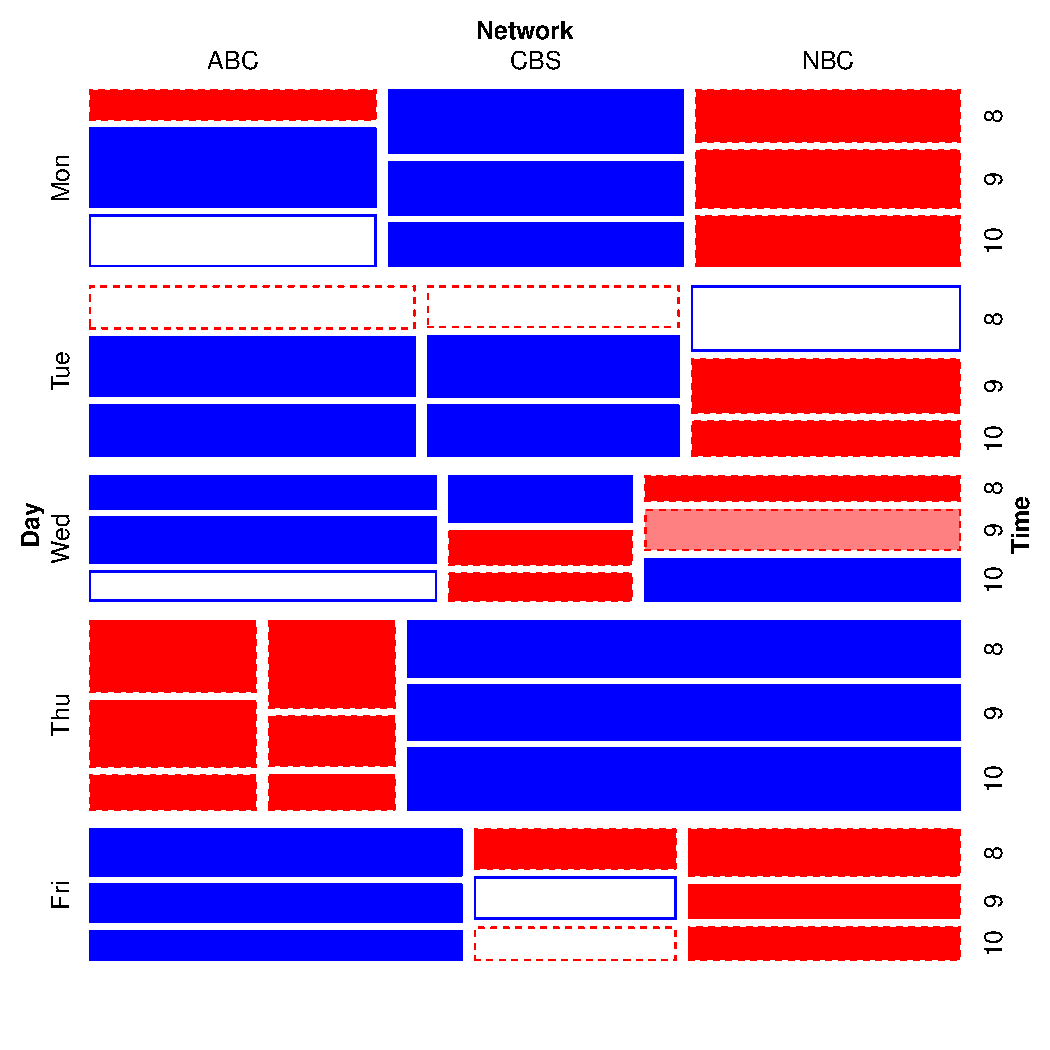
\includegraphics[width=.75\textwidth]{ch02/fig/TV-mosaic-1} }

\caption[Mosaic plot for the TV data]{Mosaic plot for the TV data showing model of joint independence, \texttt{Day:Time + Network}\label{fig:TV-mosaic}}
\end{figure}


\end{knitrout}
\noindent
The cells shaded in blue show positive associations (observed frequency $>$ expected) and red shows negative associations.  From this it is easy to read
how network choice varies with day and
time. For example, CBS dominates in all time slots on Monday;
ABC and NBC dominate on Tuesday, particularly in the later time slots;
Thursday is an NBC day, while on Friday, ABC gets the greatest share.
\ixeoff{TV viewing data}

\section{Further reading}\label{sec:ch02-reading}

If you're new to the \R language but keen to get started with linear modeling or logistic regression in the language, take a look at this \emph{Introduction to R},
\url{http://data.princeton.edu/R/introducingR.pdf},
by Germ\'an Rodr\'iguez.

\section{Lab exercises}\label{sec:ch02-exercises}

\begin{Exercises}

\exercise The packages \pkg{vcd} and \pkg{vcdExtra} contain many data sets with some
examples of analysis and graphical display.  The goal of this exercise is to
familiarize yourself with these resources.

You can get a brief summary of
these using the function \func{datasets}.  Use the following to get a list of
these with some characteristics and titles.
\begin{knitrout}\footnotesize
\definecolor{shadecolor}{rgb}{1, 0.961, 0.933}\color{fgcolor}\begin{kframe}
\begin{alltt}
\hlstd{ds} \hlkwb{<-} \hlkwd{datasets}\hlstd{(}\hlkwc{package}\hlstd{=}\hlkwd{c}\hlstd{(}\hlstr{"vcd"}\hlstd{,} \hlstr{"vcdExtra"}\hlstd{))}
\hlkwd{str}\hlstd{(ds)}
\end{alltt}
\begin{verbatim}
## 'data.frame':	70 obs. of  5 variables:
##  $ Package: chr  "vcd" "vcd" "vcd" "vcd" ...
##  $ Item   : chr  "Arthritis" "Baseball" "BrokenMarriage" "Bundesliga" ...
##  $ class  : chr  "data.frame" "data.frame" "data.frame" "data.frame" ...
##  $ dim    : chr  "84x5" "322x25" "20x4" "14018x7" ...
##  $ Title  : chr  "Arthritis Treatment Data" "Baseball Data" "Broken Marriage Data" "Ergebnisse der Fussball-Bundesliga" ...
\end{verbatim}
\end{kframe}
\end{knitrout}
  \begin{enumerate*}
    \item How many data sets are there altogether?  How many are there in each package?
    \item Make a tabular display of the frequencies by \code{Package} and \code{class}.
    \item Choose one or two data sets from this list, and examine their help files
    (e.g., \code{help(Arthritis)} or \code{?Arthritis}).  You can use, e.g.,
    \code{example(Arthritis)} to run the \R code for a given example.
  \end{enumerate*}

\exercise The data set \data{UCBADdmissions} is a 3-way table of frequencies
classified by \var{Admit}, \var{Gender} and \var{Dept}.
  \begin{enumerate*}
    \item Find the total number of cases contained in this table.
    \item For each department, find the total number of applicants.
    \item For each department, find the overall proportion of applicants who were admitted.
    \item Construct a tabular display of department (rows) and gender (columns), showing
    the proportion of applicants in each cell who were admitted.
  \end{enumerate*}

\exercise The data set \data{DanishWelfare} in \pkg{vcd}
gives a 4-way, $3 \times 4 \times 3 \times 5$
table as a data frame in
frequency form, containing the variable \var{Freq} and four factors,
\var{Alcohol},
\var{Income},
\var{Status} and
\var{Urban}.  The variable \var{Alcohol} can be considered as the
response variable, and the others as possible predictors.

  \begin{enumerate*}
    \item Find the total number of cases represented in this table.
    \item In this form, the variables \var{Alcohol} and \var{Income}
    should arguably be considered \emph{ordered} factors.  Change them
    to make them ordered.
    \item Convert this data frame to table form, \code{DanishWelfare.tab},
    a 4-way array containing the
    frequencies with appropriate variable names and level names.
    \item The variable \var{Urban} has 5 categories.  Find the total frequencies
    in each of these.  How would you collapse the table to have only
    two categories, \code{City}, \code{Non-city}?
    \item Use \func{structable} or \func{ftable} to produce a pleasing
    flattened display of the frequencies in the 4-way table.  Choose the
    variables used as row and column variables to make it easier to compare
    levels of \var{Alcohol} across the other factors.
  \end{enumerate*}

\exercise The data set \data{UKSoccer} in \pkg{vcd} gives the distributions of
number of goals scored by the 20 teams in the  1995/96 season of the
Premier League of the UK Football Association.
\begin{knitrout}
\definecolor{shadecolor}{rgb}{1, 0.961, 0.933}\color{fgcolor}\begin{kframe}
\begin{alltt}
\hlkwd{data}\hlstd{(UKSoccer,} \hlkwc{package}\hlstd{=}\hlstr{"vcd"}\hlstd{)}
\hlkwd{ftable}\hlstd{(UKSoccer)}
\end{alltt}
\begin{verbatim}
##      Away  0  1  2  3  4
## Home                    
## 0         27 29 10  8  2
## 1         59 53 14 12  4
## 2         28 32 14 12  4
## 3         19 14  7  4  1
## 4          7  8 10  2  0
\end{verbatim}
\end{kframe}
\end{knitrout}
This two-way table classifies all $20 \times 19 = 380$ games by the joint
outcome (Home, Away), the number of goals scored by the \code{Home} and
\code{Away} teams.
The value \code{4} in this table actually represents 4 or more goals.

  \begin{enumerate*}
    \item Verify that the total number of games represented in this table is 380.
    \item Find the marginal total of the number of goals scored by each of
    the home and away teams.
    \item Express each of the marginal totals as proportions.
    \item Comment on the distribution of the numbers of home-team and away-team
    goals.  Is there any evidence that home teams score more goals on average?

  \end{enumerate*}

\exercise The one-way frequency table, \data{Saxony} in \pkg{vcd} records the frequencies
of families with 0, 1, 2, $\dots$ 12 male children, among 6115 families with 12
children.  This data set is used extensively in \chref{ch:discrete}.
\begin{knitrout}
\definecolor{shadecolor}{rgb}{1, 0.961, 0.933}\color{fgcolor}\begin{kframe}
\begin{alltt}
\hlkwd{data}\hlstd{(Saxony,} \hlkwc{package}\hlstd{=}\hlstr{"vcd"}\hlstd{)}
\hlstd{Saxony}
\end{alltt}
\begin{verbatim}
## nMales
##    0    1    2    3    4    5    6    7    8    9   10   11   12 
##    3   24  104  286  670 1033 1343 1112  829  478  181   45    7
\end{verbatim}
\end{kframe}
\end{knitrout}
Another data set, \data{Geissler} in the \Rpackage{vcdExtra}, gives the complete
tabulation of all combinations of \code{boys} and \code{girls} in families with
a given total number of children \code{size}.  The task here is to create an
equivalent table, \code{Saxony12} from the \data{Geissler} data.
\begin{knitrout}
\definecolor{shadecolor}{rgb}{1, 0.961, 0.933}\color{fgcolor}\begin{kframe}
\begin{alltt}
\hlkwd{data}\hlstd{(Geissler,} \hlkwc{package}\hlstd{=}\hlstr{"vcdExtra"}\hlstd{)}
\hlkwd{str}\hlstd{(Geissler)}
\end{alltt}
\begin{verbatim}
## 'data.frame':	90 obs. of  4 variables:
##  $ boys : int  0 0 0 0 0 0 0 0 0 0 ...
##  $ girls: num  1 2 3 4 5 6 7 8 9 10 ...
##  $ size : num  1 2 3 4 5 6 7 8 9 10 ...
##  $ Freq : int  108719 42860 17395 7004 2839 1096 436 161 66 30 ...
\end{verbatim}
\end{kframe}
\end{knitrout}
  \begin{enumerate*}
    \item Use \func{subset} to create a data frame, \code{sax12} containing
    the \data{Geissler} observations in families with \code{size==12}.
    \item Select the columns for \code{boys} and \code{Freq}.
    \item Use \func{xtabs} with a formula, \verb|Freq ~ boys|, to create the
    one-way table.
    \item Do the same steps again, to create a one-way table, \code{Saxony11}
    containing similar frequencies for families of \code{size==11}.
  \end{enumerate*}

\exercise \emph{Interactive coding of table factors}:  Some statistical and graphical
\hard
methods for \ctabs are implemented only for two-way tables, but can be extended
to 3+ way tables by recoding the factors to interactive combinations along the
rows and/or columns, in a way similar to what \func{ftable} and \func{structable}
do for printed displays.

For the \data{UCBAdmissions} data, produce a two-way table object, \code{UCB.tab2}
that has the combinations of \var{Admit} and \var{Gender} as the rows, and
\var{Dept} as its columns, to look like the result below:
\begin{verbatim}
                 Dept
Admit:Gender        A   B   C   D   E   F
  Admitted:Female  89  17 202 131  94  24
  Admitted:Male   512 353 120 138  53  22
  Rejected:Female  19   8 391 244 299 317
  Rejected:Male   313 207 205 279 138 351
\end{verbatim}
\emph{Hint}: convert to a data frame, manipulate the factors, then convert back to
a table.

\exercise The data set \data{VisualAcuity} in \pkg{vcd} gives $4 \times 4 \times 2$
table as a frequency data frame.
\begin{knitrout}
\definecolor{shadecolor}{rgb}{1, 0.961, 0.933}\color{fgcolor}\begin{kframe}
\begin{alltt}
\hlkwd{data}\hlstd{(}\hlstr{"VisualAcuity"}\hlstd{,} \hlkwc{package}\hlstd{=}\hlstr{"vcd"}\hlstd{)}
\hlkwd{str}\hlstd{(VisualAcuity)}
\end{alltt}
\begin{verbatim}
## 'data.frame':	32 obs. of  4 variables:
##  $ Freq  : num  1520 234 117 36 266 ...
##  $ right : Factor w/ 4 levels "1","2","3","4": 1 2 3 4 1 2 3 4 1 2 ...
##  $ left  : Factor w/ 4 levels "1","2","3","4": 1 1 1 1 2 2 2 2 3 3 ...
##  $ gender: Factor w/ 2 levels "male","female": 2 2 2 2 2 2 2 2 2 2 ...
\end{verbatim}
\end{kframe}
\end{knitrout}
  \begin{enumerate*}
    \item From this, use \func{xtabs} to create two $4\times 4$ frequency tables, one for
each gender.
    \item Use \func{structable} to create a nicely organized tabular display.
    \item Use \func{xtable} to create a \LaTeX\ or HTML table.
  \end{enumerate*}

\end{Exercises}


%\TODO{Cleanup some local variables}





\chapter{Fitting and graphing discrete distributions}\label{ch:discrete}
%\begin{center}
 \rule[-4pt]{0.5pt}{4pt}\hrulefill\rule[-4pt]{0.5pt}{4pt}\\
 \begin{minipage}[c]{.33\linewidth}
  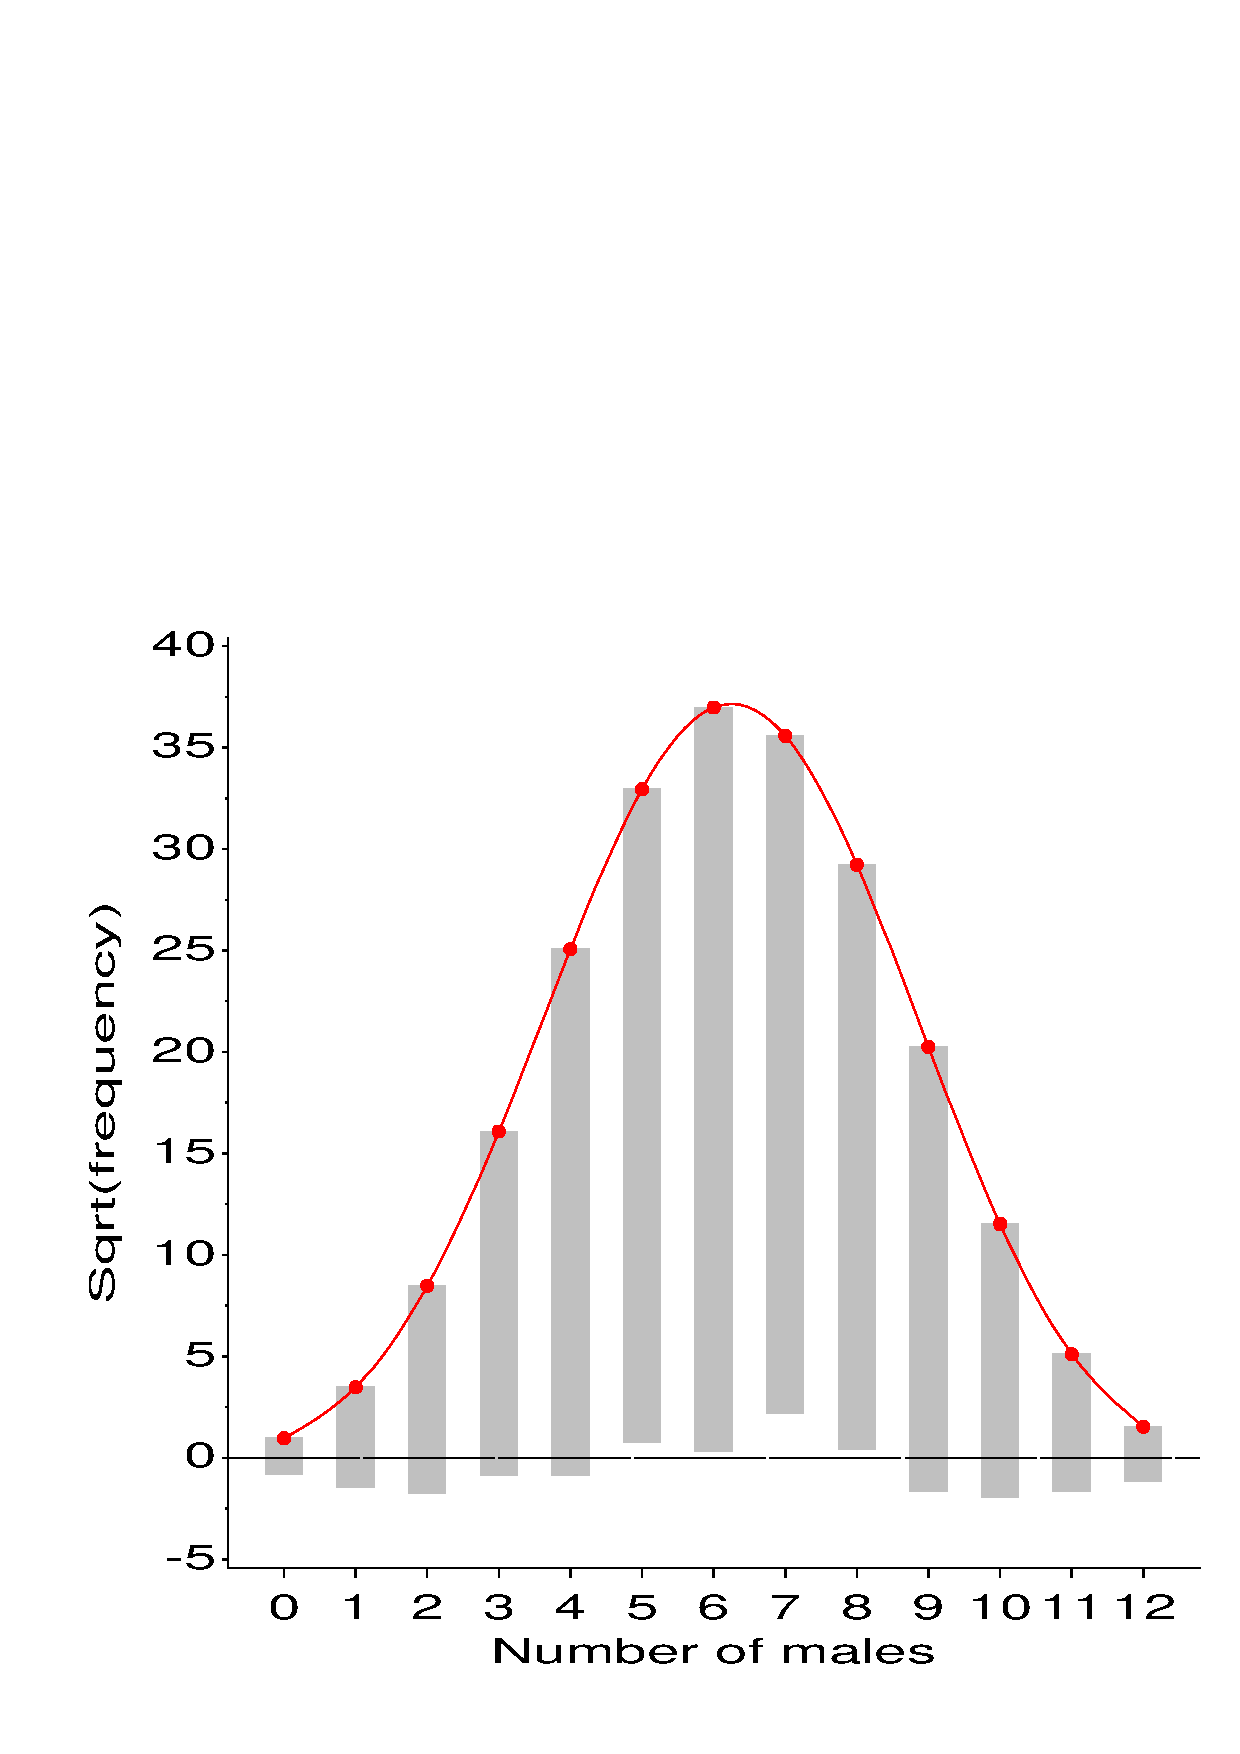
\includegraphics[width=1\linewidth]{saxony}\graphicsfile{ch2/fig/saxony.eps}{}
 \end{minipage}%
 \hfill
 \begin{minipage}[c]{.33\linewidth}
  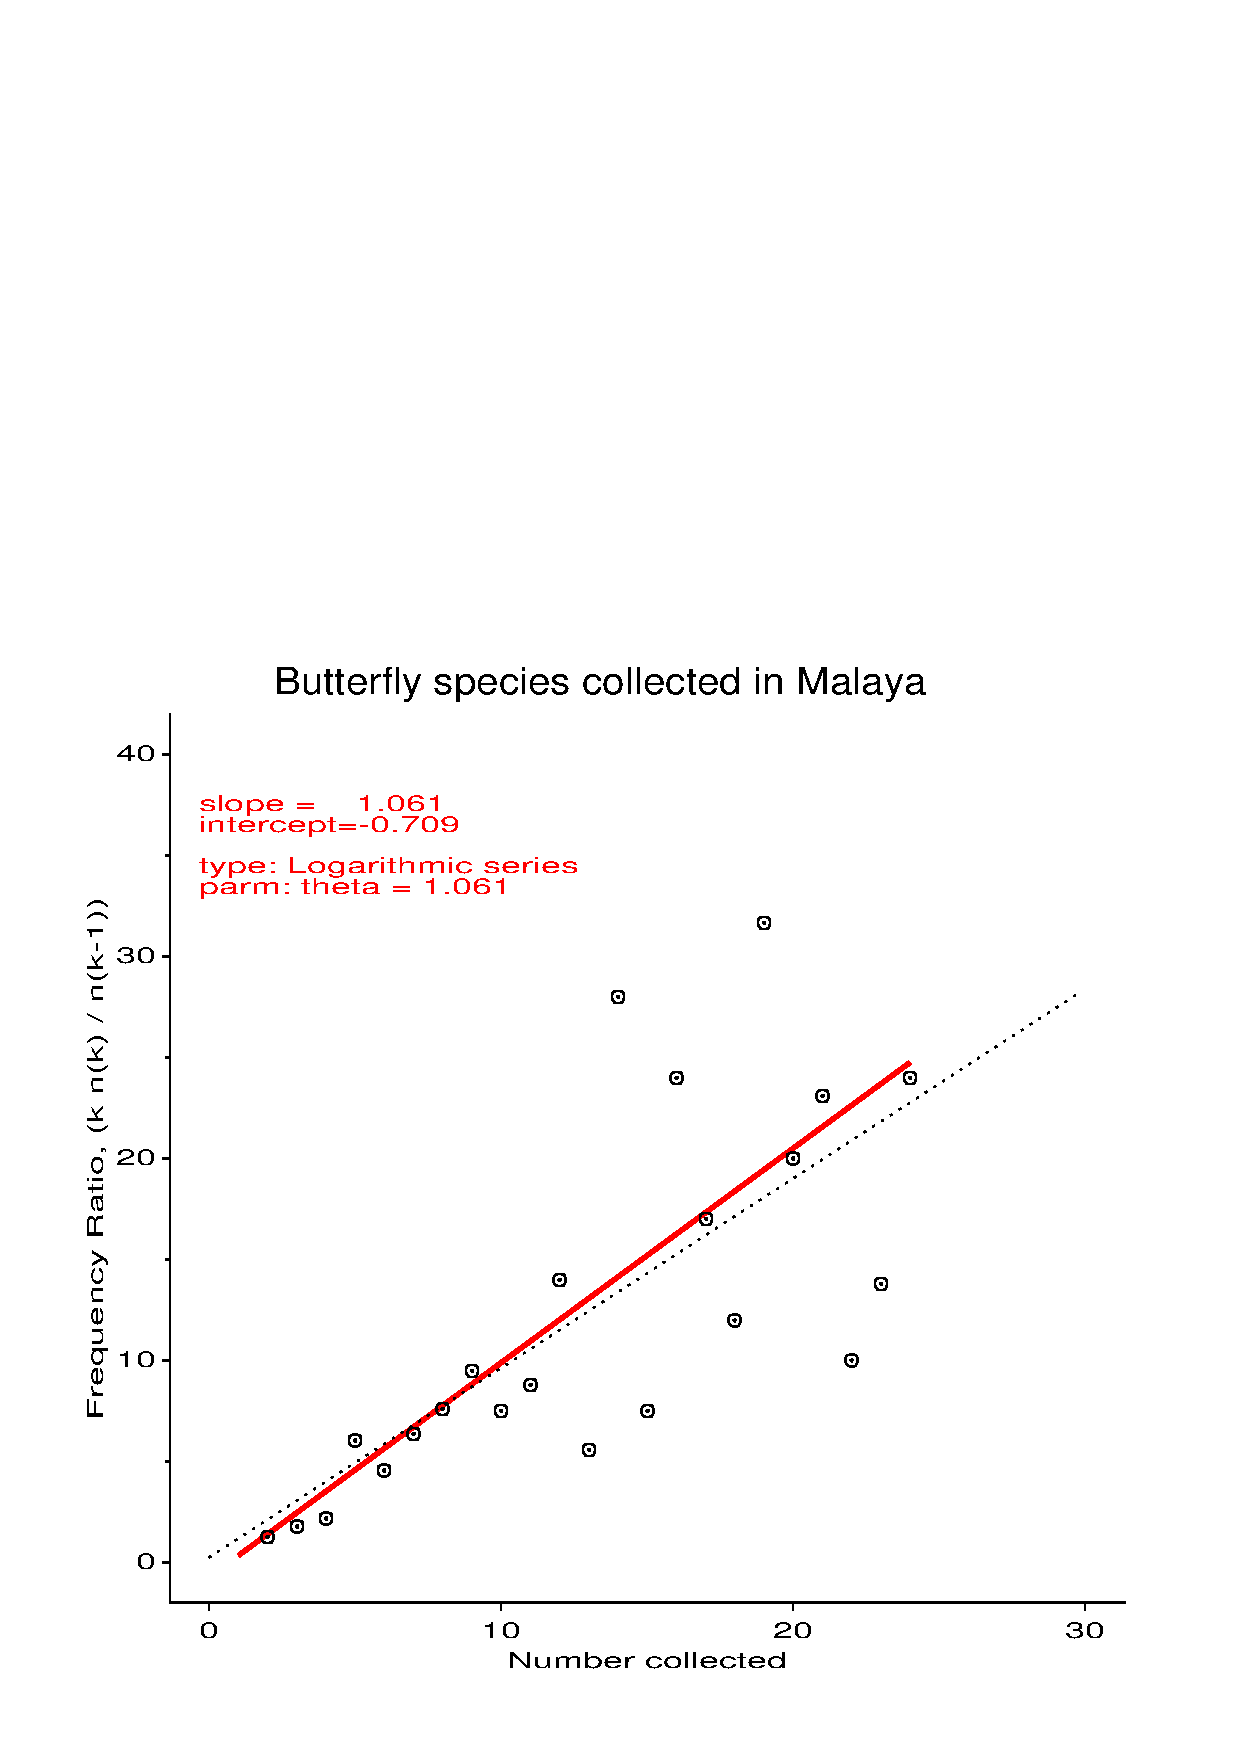
\includegraphics[width=1\linewidth]{orddemo3}\graphicsfile{ch2/fig/orddemo3.eps}{}
 \end{minipage}
 \hfill
 \begin{minipage}[c]{.33\linewidth}
  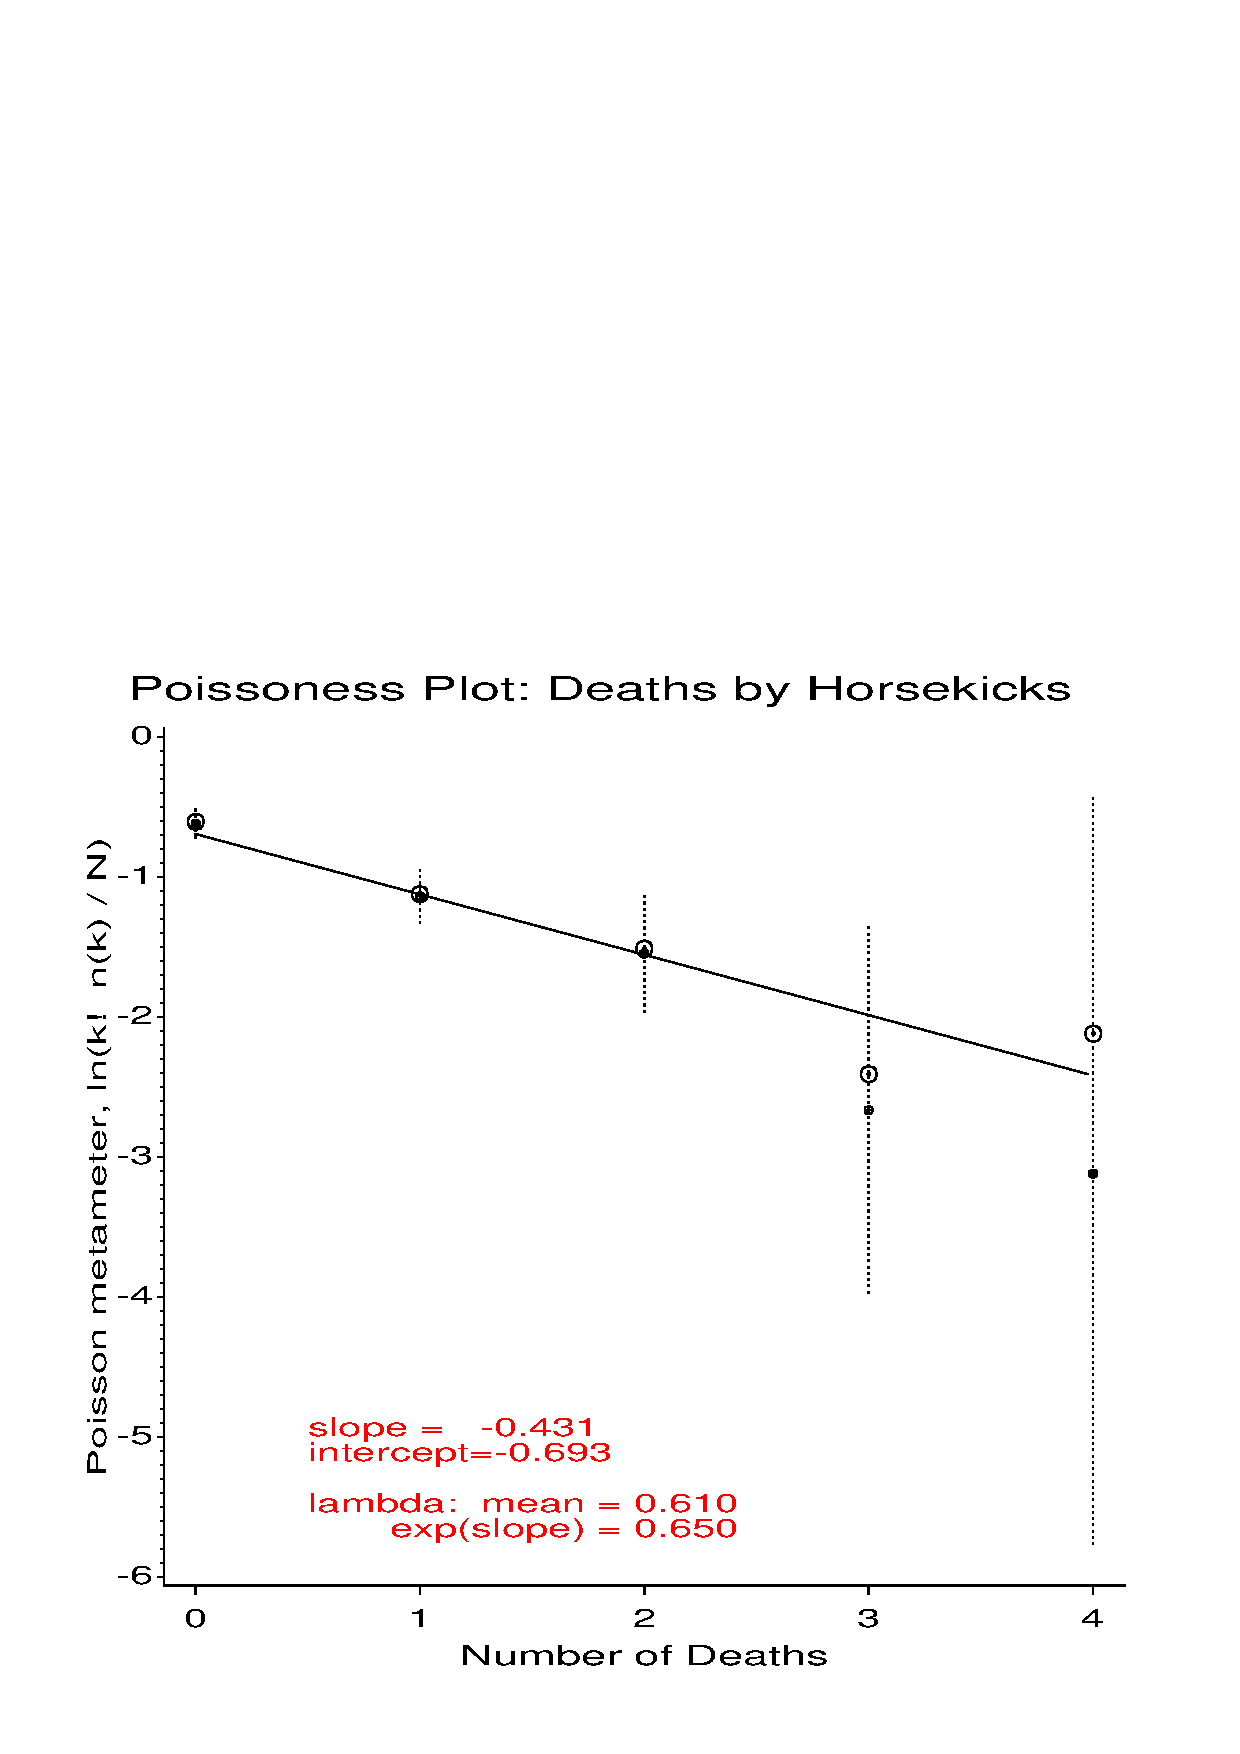
\includegraphics[width=1\linewidth]{poisdemo1}\graphicsfile{ch2/fig/poisdemo1.eps}{}
 \end{minipage}
\end{center}

   %% visual contents images

\chapterprelude{
Discrete data often follow various theoretical probability models.
Graphic displays are used to visualize goodness of fit,
to diagnose an appropriate model, and determine the impact of
individual observations on estimated parameters.
}
% \minitoc
% \clearpage

\epigraph{Not everything that counts can be counted, and not everything that
can be counted counts.}
{Albert Einstein}

Discrete frequency distributions often involve counts of occurrences of events,
such as accident fatalities, incidents of terrorism or suicide,
words in passages of text, or blood cells with some characteristic.
Often interest is focused on how closely such data follow a particular probability distribution,
such as the binomial, Poisson, or geometric distribution, which
provide the basis for generating mechanisms that might give rise to the
data.
Understanding and visualizing
such distributions
in the simplest case of an unstructured sample provides a building block for generalized
linear models (\chref{ch:glm}) where they serve as one component.  The also provide the basis for
a variety of recent extensions of regression models for count data (Chapter ?),
allowing excess counts of zeros (zero-inflated models), left- or right-
truncation often encountered in statistical practice.

This chapter describes the well-known discrete
frequency distributions: the binomial, Poisson, negative binomial,
geometric, and logarithmic series distributions in the simplest case of an unstructured sample.
The chapter begins with simple graphical displays (line graphs and bar charts) to view
the distributions of empirical data and theoretical frequencies from a specified
discrete distribution.

It then describes methods for fitting data to a distribution of a given form
and simple, effective
graphical methods than can be used to visualize goodness of fit,
to diagnose an appropriate model (e.g., does a given data set follow the
Poisson or negative binomial?) and determine the impact of
individual observations on estimated parameters.

\section{Introduction to discrete distributions}\label{sec:discrete-intro}
Discrete data analysis is concerned with the study of the tabulation of one or
more types of events, often categorized into mutually exclusive and exhaustive
categories.  \term{Binary events} having two outcome categories include
the toss of a coin (head/tails), sex of a child (male/female), survival of
a patient following surgery (lived/died), and so forth.  \term{Polytomous events}
have more outcome categories, which may be \emph{ordered}
(rating of impairment: low/medium/high, by a physician)
and possibly numerically-valued
(number of dots (pips), 1--6 on the toss of a die)
or \emph{unordered} (political party supported: Liberal, Conservative, Greens, Socialist).

In this chapter, we focus largely on one-way frequency tables for a single
numerically-valued variable.
Probability models for such data provide the opportunity to describe or explain
the \emph{structure} in such data, in that they entail some data generating
mechanism and provide the basis for testing scientific hypotheses, prediction of
future results.  If a given probability model does not fit the data, this can often
be a further opportunity to extend understanding of the data or the underlying
substantive theory or both.

The remainder of this section gives a few substantive examples of situations where the
well-known discrete frequency distributions (binomial, Poisson, negative binomial,
geometric, and logarithmic series) might reasonably apply, at least approximately.
The mathematical characteristics and properties of these theoretical
distributions are postponed to \secref{sec:discrete-distrib}.

In many cases, the data at hand pertain to two types of variables in a one-way
frequency table. There is a basic outcome variable, $k$, taking integer values,
$k = 0, 1, \dots$, and called a \term{count}.  For each value of $k$, we also have
a \term{frequency}, $n_k$ that the count $k$ was observed in some sample.
For example, in the study of children in families, the count variable
$k$ could be the total number of children or the number of male children;
the frequency variable, $n_k$, would then give the number of families with that
basic count $k$.

\subsection{Binomial data}\label{sec:binom-data}
Binomial type data arise as the discrete distribution of the number of
``success'' events in $n$ independent binary trials, each of which
yields a success (yes/no, head/tail, lives/dies, male/female) with a constant probability $p$.

Sometimes, as in \exref{ex:arbuthnot1}
below, the available data record only the number of successes
in $n$ trials, with separate such observations recorded over
time or space.  More commonly, as in \exref{ex:saxony1}
and \exref{ex:dice},
we have available data on the frequency $n_k$
of $k = 0, 1, 2, \dots n$ successes in the $n$ trials.


\begin{Example}[arbuthnot1]{Arbuthnot data}
Sex ratios--- births of male to female children have long been of interest
in population studies and demography. Indeed, in 1710, John Arbuthnot \citep{Arbuthnot:1710}
used data on the ratios of male to female christenings in London from 1629--1710 to carry out the first known significance test.
The data for these 82 years showed that in \emph{every} year there were more boys than girls.
He calculated that the under the assumption
that male and female births were equally likely, the probability of 82 years of
more males than females was vanishingly small,
 ($\Pr \approx 4.14 \times 10^{-25}$).
He used this to argue that a nearly constant birth ratio $> 1$ (or $\Pr(\mathrm{Male}) > 0.5$)
could be interpreted to show the guiding hand of a divine being.

Arbuthnot's data, along with some other related variables
are available in \data{Arbuthnot} in the \Rpackage{HistData}.
For now, we simply display a plot of the probability of a male birth over time.
The plot in \figref{fig:arbuthnot1} shows the proportion of males over years,
with horizontal lines at $\Pr(\mathrm{Male}) = 0.5$ and the mean,
$\Pr(\mathrm{Male}) = 0.517$.  Also shown is a (loess) smoothed curve, which suggests
that any deviation from a constant sex ratio is relatively small.
\begin{knitrout}
\definecolor{shadecolor}{rgb}{1, 0.961, 0.933}\color{fgcolor}\begin{kframe}
\begin{alltt}
\hlkwd{data}\hlstd{(Arbuthnot,} \hlkwc{package}\hlstd{=}\hlstr{"HistData"}\hlstd{)}
\hlkwd{with}\hlstd{(Arbuthnot, \{}
  \hlstd{prob} \hlkwb{=} \hlstd{Males}\hlopt{/}\hlstd{(Males}\hlopt{+}\hlstd{Females)}
  \hlkwd{plot}\hlstd{(Year, prob,} \hlkwc{type}\hlstd{=}\hlstr{'b'}\hlstd{,} \hlkwc{ylim}\hlstd{=}\hlkwd{c}\hlstd{(}\hlnum{0.5}\hlstd{,} \hlnum{0.54}\hlstd{),} \hlkwc{ylab}\hlstd{=}\hlstr{"Pr (Male)"}\hlstd{)}
  \hlkwd{abline}\hlstd{(}\hlkwc{h}\hlstd{=}\hlnum{0.5}\hlstd{,} \hlkwc{col}\hlstd{=}\hlstr{"red"}\hlstd{,} \hlkwc{lwd}\hlstd{=}\hlnum{2}\hlstd{)}
  \hlkwd{abline}\hlstd{(}\hlkwc{h}\hlstd{=}\hlkwd{mean}\hlstd{(prob),} \hlkwc{col}\hlstd{=}\hlstr{"blue"}\hlstd{)}
  \hlkwd{text}\hlstd{(}\hlkwc{x}\hlstd{=}\hlnum{1640}\hlstd{,} \hlkwc{y}\hlstd{=}\hlnum{0.5}\hlstd{,} \hlkwd{expression}\hlstd{(H[}\hlnum{0}\hlstd{]}\hlopt{:} \hlstr{"Pr(Male)=0.5"}\hlstd{),} \hlkwc{pos}\hlstd{=}\hlnum{3}\hlstd{,} \hlkwc{col}\hlstd{=}\hlstr{"red"}\hlstd{)}
  \hlstd{Arb.smooth} \hlkwb{<-} \hlkwd{loess.smooth}\hlstd{(Year,prob)}
  \hlkwd{lines}\hlstd{(Arb.smooth}\hlopt{$}\hlstd{x, Arb.smooth}\hlopt{$}\hlstd{y,} \hlkwc{col}\hlstd{=}\hlstr{"blue"}\hlstd{,} \hlkwc{lwd}\hlstd{=}\hlnum{2}\hlstd{)}
  \hlstd{\})}
\end{alltt}
\end{kframe}\begin{figure}[!htbp]


\centerline{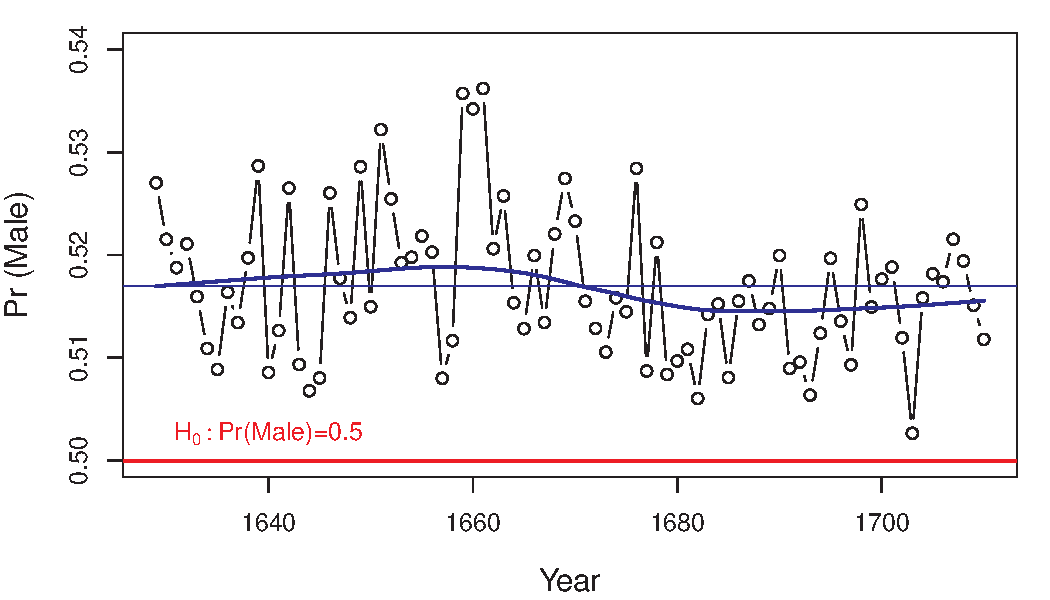
\includegraphics[width=.75\textwidth]{ch03/fig/arbuthnot1-1} }

\caption[Arbuthnot's data on male/female sex ratios]{Arbuthnot's data on male/female sex ratios in London, 1629--1710, together with a (loess) smoothed curve over time and the mean Pr(Male)\label{fig:arbuthnot1}}
\end{figure}


\end{knitrout}
We return to this data in a later chapter where we ask whether the variation around
the mean can be explained by any other considerations, or should just be considered
random variation (see \labref{lab:7.1})
\end{Example}

\begin{Example}[saxony1]{Families in Saxony}
A related example of sex ratio data that ought to follow a binomial distribution
comes from a classic study by A. Geissler \citeyearpar{Geissler:1889}.
Geissler listed the data on the distributions of boys and girls in families
in Saxony for the period 1876--1885. In total, over four million births were
recorded, and the sex distribution in the family was available because the parents had to state the sex of all their children on
the birth certificate.%

The complete data, classified by number of boys and number of girls
(each 0--12) appear in \citet[Table 1]{Edwards:1958}.%
\footnote{
\citet{Edwards:1958} notes that over these 10 years, many parents
will have had several children, and their family composition
is therefore recorded more than once.  However, in families with a given
number of children, each family can appear only once.
}
\citet[Table 6.2]{Lindsey:95} selected only the 6115 families with
12 children, and listed the frequencies by number of males.  The
data are shown in table form in \tabref{tab:saxtab} in the standard form
of a complete discrete distribution.  The basic outcome variable,
$k = 0, 1, \dots, 12$, is the number of male children in a family
and the frequency variable, $n_k$ is the number of families with that
number of boys.

% latex table generated in R 3.0.1 by xtable 1.7-1 package
% Tue Nov 26 14:56:02 2013
\begin{table}[ht]
\caption{Number of male children in 6115 Saxony families of size 12} \label{tab:saxtab}
\centering
\begin{tabular}{l|rrrrrrrrrrrrrr}
  \hline
Males ($k$) & 0 & 1 & 2 & 3 & 4 & 5 & 6 & 7 & 8 & 9 & 10 & 11 & 12 & Sum \\ 
  \hline
Families ($n_k$) & 3 & 24 & 104 & 286 & 670 & 1,033 & 1,343 & 1,112 & 829 & 478 & 181 & 45 & 7 & 6,115 \\ 
   \hline
\end{tabular}
\end{table}
 


\figref{fig:saxony-barplot} shows a bar plot of the frequencies in \tabref{tab:saxtab}.
It can be seen that the distribution is quite symmetric.  The questions of interest
here are:
(a) how close does the data follow a binomial distribution, with a constant
$\Pr(\mathrm{Male}) = p$?
(b) is there evidence to reject the hypothesis that $ p = 0.5$?

\begin{knitrout}
\definecolor{shadecolor}{rgb}{1, 0.961, 0.933}\color{fgcolor}\begin{kframe}
\begin{alltt}
\hlkwd{data}\hlstd{(Saxony,} \hlkwc{package}\hlstd{=}\hlstr{"vcd"}\hlstd{)}
\hlkwd{barplot}\hlstd{(Saxony,} \hlkwc{xlab}\hlstd{=}\hlstr{"Number of males"}\hlstd{,} \hlkwc{ylab}\hlstd{=}\hlstr{"Number of families"}\hlstd{,}
        \hlkwc{col}\hlstd{=}\hlstr{"lightblue"}\hlstd{,} \hlkwc{cex.lab}\hlstd{=}\hlnum{1.5}\hlstd{)}
\end{alltt}
\end{kframe}\begin{figure}[!htbp]


\centerline{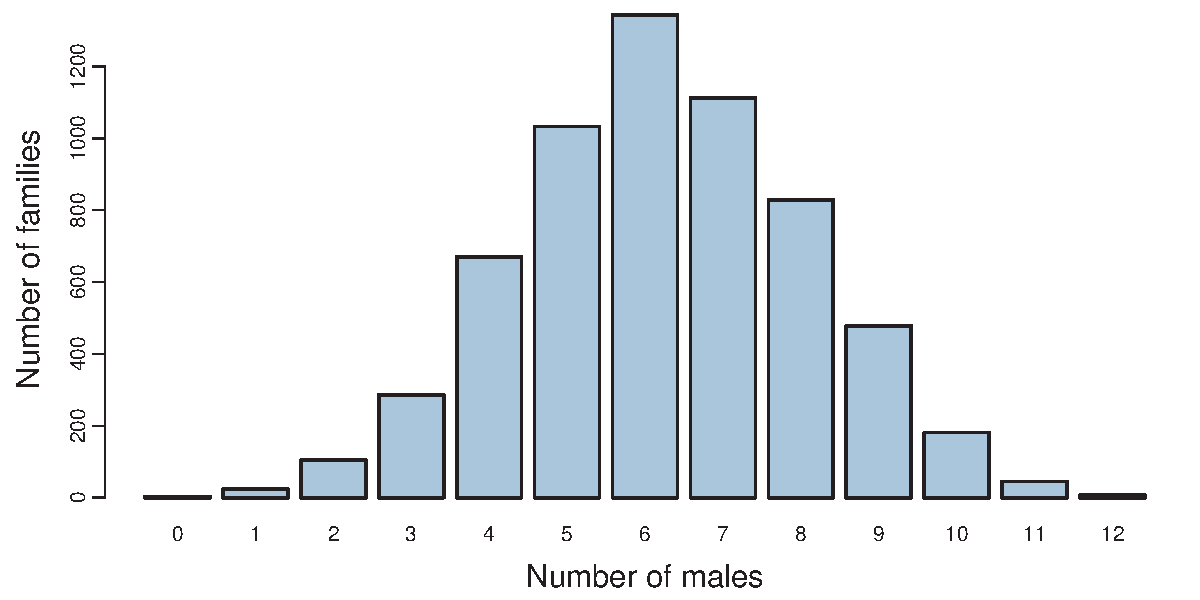
\includegraphics[width=.75\textwidth]{ch03/fig/saxony-barplot-1} }

\caption[Males in Saxony families of size 12]{Males in Saxony families of size 12\label{fig:saxony-barplot}}
\end{figure}


\end{knitrout}
\end{Example}

\begin{Example}[dice]{Weldon's dice}
Common examples of binomial distributions involve tossing coins
or dice, where some event outcome is considered a ``success''
and the number of successes ($k$) are tabulated
in a long series of trials to give the frequency ($n_k$)
of each basic count, $k$.

Perhaps the most industrious dice-tosser of all times,
W. F. Raphael Weldon, an English evolutionary biologist
and joint founding editor of \emph{Biometrika} (with Francis Galton and Karl Pearson)
tallied the results of throwing 12 dice 26,306 times.
For his purposes, he considered the outcome of 5 or 6 pips showing on each die
to be a success to be a success, and all other outcomes as failures.

Weldon reported his results in a letter to Francis Galton dated
February 2, 1894, in order
``to judge whether the differences between a series of group frequencies
and a theoretical law \dots were more than might be attributed
to the chance fluctuations of random sampling''
\citep{KempKemp:91}.
In his seminal paper,
\citet{Pearson:00} used Weldon's data to illustrate the \chisq{} goodness-of-fit test, as did
\citet[Table 5.1, p. 121]{KendallStuart:63}.

These data are
shown here as
\tabref{tab:dicetab},
in terms of the number of occurrences of a 5 or
6 in the throw of 12 dice.
If the dice were all identical and perfectly fair (balanced), one would
expect that $p = \Pr\{5 \textrm{ or } 6\} = \frac13$
and the distribution of the number of 5 or 6 would be binomial.

A peculiar feature of these data
as presented by Kendall and Stuart (not uncommon in discrete distributions)
is that the frequencies of 10--12 successes
are lumped together.%
\footnote{
The unlumped entries are, for (number of 5s or 6s: frequency) ---
(10: 14); (11: 4), (12:0),
given by \citet{Labby:2009}.
In this remarkable paper, Labby describes a mechanical device he constructed to
repeat Weldon's experiment physically and automate the counting of outcomes.
He created electronics to roll 12 dice in a physical box, and hooked that
up to a webcam to capture an image of each toss and used image processing
software to record the counts.
}
This grouping must be taken into account in fitting
the distribution.  This dataset is available as \data{WeldonDice} in the
\Rpackage{vcd}.  The distribution is plotted in \figref{fig:dice}.

% latex table generated in R 3.0.1 by xtable 1.7-1 package
% Thu Nov 28 15:27:53 2013
\begin{table}[ht]
\centering
\caption{Frequencies of 5s or 6s in throws of 12 dice} \label{tab:dicetab}
\begin{tabular}{l|rrrrrrrrrrrr}
   \hline
\# 5s or 6s ($k$) & 0 & 1 & 2 & 3 & 4 & 5 & 6 & 7 & 8 & 9 & 10+ & Sum \\ 
Frequency ($n_k$) &   185 &  1,149 &  3,265 &  5,475 &  6,114 &  5,194 &  3,067 &  1,331 &   403 &   105 &    18 & 26,306 \\ 
   \hline
\end{tabular}
\end{table}



%%% one figure
%\begin{figure}[htb]
%%  \SASfig{dice.eps}{scale=.65}{dice}{Weldon's dice data}
%  \centering
%  \includegraphics[scale=.65]{dice.eps}
%  \caption{Weldon's dice data}%
%  \label{fig:dice}
%\end{figure}

\begin{knitrout}
\definecolor{shadecolor}{rgb}{1, 0.961, 0.933}\color{fgcolor}\begin{kframe}
\begin{alltt}
\hlkwd{data}\hlstd{(WeldonDice,} \hlkwc{package}\hlstd{=}\hlstr{"vcd"}\hlstd{)}
\hlkwd{dimnames}\hlstd{(WeldonDice)}\hlopt{$}\hlstd{n56[}\hlnum{11}\hlstd{]} \hlkwb{<-} \hlstr{"10+"}
\hlkwd{barplot}\hlstd{(WeldonDice,} \hlkwc{xlab}\hlstd{=}\hlstr{"Number of 5s and 6s"}\hlstd{,} \hlkwc{ylab}\hlstd{=}\hlstr{"Frequency"}\hlstd{,}
        \hlkwc{col}\hlstd{=}\hlstr{"lightblue"}\hlstd{,} \hlkwc{cex.lab}\hlstd{=}\hlnum{1.5}\hlstd{)}
\end{alltt}
\end{kframe}\begin{figure}[!htbp]


\centerline{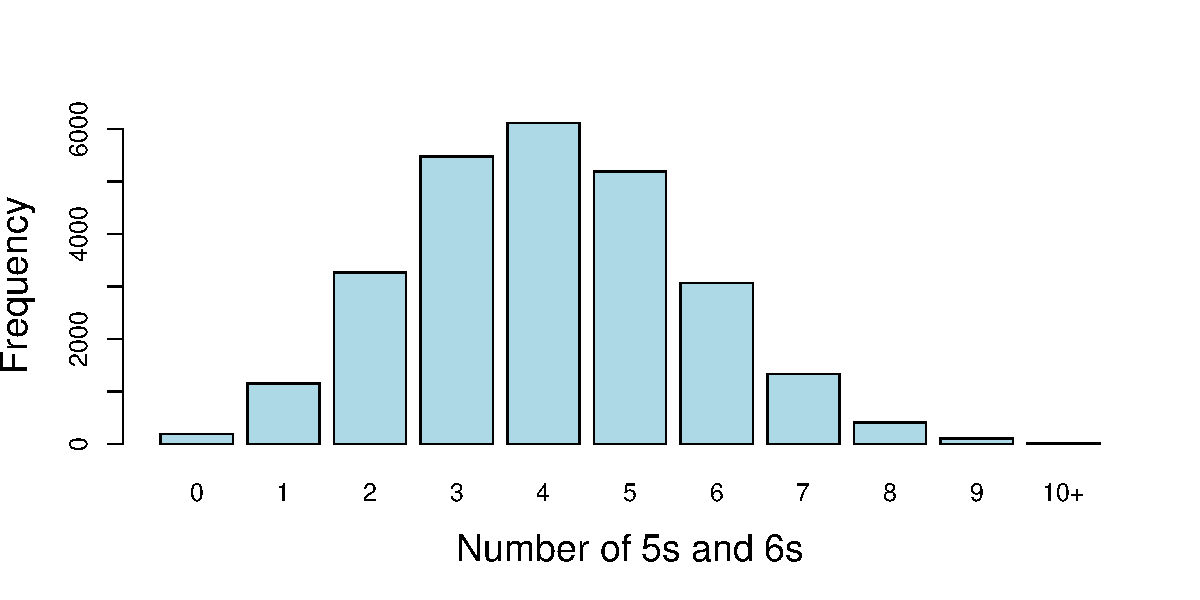
\includegraphics[width=.75\textwidth]{ch03/fig/dice-1} }

\caption[Weldon's dice data]{Weldon's dice data\label{fig:dice}}
\end{figure}


\end{knitrout}
\end{Example}

\subsection{Poisson data}\label{sec:pois-data}

Data of Poisson type arise when we observe the counts of events $k$ within a
fixed interval of time or space (length, area, volume) and tabulate their
frequencies, $n_k$.  For example, we may observe the number of radioactive
particles emitted by a source per second or number of births per hour,
or the number of tiger or whale sightings within some geographical regions.

In contrast to binomial data, where the counts are bounded below and above,
in Poisson data the counts $k$ are bounded below at 0, but can take integer
values with no fixed upper limit.
One defining characteristic for the Poisson distribution is for rare
events, which occur independently with a small and constant probability, $p$
in small intervals, and we count the number of such occurrences.

Several examples of data of this general type are given below.

\begin{Example}[horskick1]{Death by horse kick}
One of the oldest and best known examples of a Poisson distribution
is the data from
\citet{Bortkiewicz:98} on deaths of soldiers in the Prussian
army from kicks by horses and mules, shown in \tabref{tab:horsetab}.
Ladislaus von Bortkiewicz, an economist and statistician,
tabulated the number of soldiers in each of
14 army corps in the 20 years from 1875-1894
who died after being kicked by a horse
\citep[p. 18]{AndrewsHerzberg:85}.
\tabref{tab:horsetab} shows the data used by
\citet{Fisher:25} for 10 of these
army corps, summed over 20 years, giving 200
`corps-year' observations.  In 109 corps-years,
no deaths occurred; 65 corps-years had one death, etc.

The data set is available as \data{HorseKicks} in the \Rpackage{vcd}.
The distribution is plotted in \figref{fig:horsekicks}.
% latex table generated in R 3.0.1 by xtable 1.7-1 package
% Fri Nov 29 08:56:45 2013
\begin{table}[ht]
\centering
\caption{von Bortkiewicz's data on deaths by horse kicks} \label{tab:horsetab}
\begin{tabular}{l|rrrrr|r}
   \hline
Number of deaths ($k$) & 0 & 1 & 2 & 3 & 4 & Sum \\ 
  Frequency ($n_k$) & 109 &  65 &  22 &   3 &   1 & 200 \\ 
   \hline
\end{tabular}
\end{table}


\begin{knitrout}
\definecolor{shadecolor}{rgb}{1, 0.961, 0.933}\color{fgcolor}\begin{kframe}
\begin{alltt}
\hlkwd{data}\hlstd{(HorseKicks,} \hlkwc{package}\hlstd{=}\hlstr{"vcd"}\hlstd{)}
\hlkwd{barplot}\hlstd{(HorseKicks,} \hlkwc{xlab}\hlstd{=}\hlstr{"Number of deaths"}\hlstd{,} \hlkwc{ylab}\hlstd{=}\hlstr{"Frequency"}\hlstd{,}
        \hlkwc{col}\hlstd{=}\hlstr{"lightblue"}\hlstd{,} \hlkwc{cex.lab}\hlstd{=}\hlnum{1.5}\hlstd{)}
\end{alltt}
\end{kframe}\begin{figure}[!htbp]


\centerline{\includegraphics[width=.75\textwidth]{ch03/fig/horsekicks-1} }

\caption[HorseKicks data]{HorseKicks data\label{fig:horsekicks}}
\end{figure}


\end{knitrout}
\end{Example}

\begin{Example}[madison1]{Federalist papers}
In 1787--1788, Alexander Hamilton, John Jay, and James Madison
wrote a series of newspaper essays to persuade the voters of
New York State to ratify the U.S. Constitution.
The essays were titled \emph{The Federalist Papers}
and all were signed with the pseudonym ``Publius.''  Of the 77 papers published,
the author(s) of 65 are known, but \emph{both}
Hamilton and Madison later claimed sole authorship of the remaining 12.
\citet{MostellerWallace:63,MostellerWallace:84}
investigated the use of statistical methods to identify authors of
disputed works based on the frequency distributions of certain key
function words, and concluded that Madison had indeed authored the
12 disputed papers.%
\footnote{
It should be noted that this is a landmark work in the development and
application of statistical methods to the analysis of texts and
cases of disputed authorship. In addition to
\emph{may}, they considered many such marker words,
such as \emph{any}, \emph{by}, \emph{from}, \emph{upon}, and so forth.
Among these, the word \emph{upon} was the best discriminator between
the works known by Hamilton (3 per 1000 words) and Madison (1/6 per 1000 words).
In this work, they pioneered the use of Bayesian discriminant analysis,
and the use of cross-validation to assess the stability of estimates
and their conclusions.
}

\tabref{tab:fedtab} shows the distribution of the occurrence of one of
these ``marker'' words,
the
word \emph{may} in 262 blocks of text (each about 200 words long)
from issues of the \emph{Federalist Papers} and other essays known
to be written by James Madison.  Read the table as follows:
in 156 blocks, the word \emph{may}
did not occur; it occurred once in 63 blocks, etc.  The distribution
is plotted in \figref{fig:federalist}.

% latex table generated in R 3.0.1 by xtable 1.7-1 package
% Fri Nov 29 14:25:47 2013
\begin{table}[htb]
\centering
\caption{Number of occurrences of the word \emph{may} in texts written by James Madison\label{tab:fedtab}} 
\begin{tabular}{l|rrrrrrr|r}
   \hline
Occurrences of \emph{may} ($k$) & 0 & 1 & 2 & 3 & 4 & 5 & 6 & Sum \\ 
  Blocks of text ($n_k$)       & 156 &  63 &  29 &   8 &   4 &   1 &   1 & 262 \\ 
   \hline
\end{tabular}
\end{table}

\begin{knitrout}
\definecolor{shadecolor}{rgb}{1, 0.961, 0.933}\color{fgcolor}\begin{kframe}
\begin{alltt}
\hlkwd{data}\hlstd{(Federalist,} \hlkwc{package}\hlstd{=}\hlstr{"vcd"}\hlstd{)}
\hlkwd{barplot}\hlstd{(Federalist,}
        \hlkwc{xlab}\hlstd{=}\hlstr{"Occurrences of 'may'"}\hlstd{,} \hlkwc{ylab}\hlstd{=}\hlstr{"Number of blocks of text"}\hlstd{,}
        \hlkwc{col}\hlstd{=}\hlstr{"lightgreen"}\hlstd{,} \hlkwc{cex.lab}\hlstd{=}\hlnum{1.5}\hlstd{)}
\end{alltt}
\end{kframe}\begin{figure}[!htbp]


\centerline{\includegraphics[width=.75\textwidth]{ch03/fig/federalist-1} }

\caption[Mosteller and Wallace Federalist data]{Mosteller and Wallace Federalist data\label{fig:federalist}}
\end{figure}


\end{knitrout}
\end{Example}

\begin{Example}[cyclists1]{London cycling deaths}

\citet{AberdeinSpiegelhalter:2013} observed that from November 5--13, 2013,
six people were killed while cycling in London.  How unusual is this
number of deaths in less than a two-week period?
Was this a freak occurrence, or should Londoners petition for
cycling lanes and greater road safety?
To answer these question, they obtained data from the
UK Department of Transport \emph{Road Safety Data} from 2005--2012
and selected all accident fatalities of cyclists within the
cit of London.

It seems reasonable to assume that, in any short period of time, deaths of
people riding bicycles are independent events.  If, in addition,
the probability of such events is constant over this time span,
the Poisson distribution should describe the distribution of
$0, 1, 2, 3, \dots$ deaths. Then, an answer to the main question can be
given in terms of the probability of six (or more) deaths in
a comparable period of time.

Their data, comprising 208 counts of deaths in the fortnightly periods
from January 2005 to December 2012 are contained in the \Dset
\data{CyclingDeaths} in \pkg{vcdExtra}.  To work with the
distribution, we first convert this to a one-way table.

\begin{knitrout}
\definecolor{shadecolor}{rgb}{1, 0.961, 0.933}\color{fgcolor}\begin{kframe}
\begin{alltt}
\hlkwd{data}\hlstd{(}\hlstr{"CyclingDeaths"}\hlstd{,} \hlkwc{package}\hlstd{=}\hlstr{"vcdExtra"}\hlstd{)}
\hlstd{CyclingDeaths.tab} \hlkwb{<-} \hlkwd{table}\hlstd{(CyclingDeaths}\hlopt{$}\hlstd{deaths)}
\hlstd{CyclingDeaths.tab}
\end{alltt}
\begin{verbatim}
## 
##   0   1   2   3 
## 114  75  14   5
\end{verbatim}
\end{kframe}
\end{knitrout}
The maximum number of deaths was 3, which occurred in only 5 two-week periods.
The distribution is plotted in \figref{fig:cyclists2}.
\begin{knitrout}
\definecolor{shadecolor}{rgb}{1, 0.961, 0.933}\color{fgcolor}\begin{kframe}
\begin{alltt}
\hlkwd{barplot}\hlstd{(CyclingDeaths.tab,}
        \hlkwc{xlab}\hlstd{=}\hlstr{"Number of deaths"}\hlstd{,} \hlkwc{ylab}\hlstd{=}\hlstr{"Number of fortnights"}\hlstd{,}
        \hlkwc{col}\hlstd{=}\hlstr{"pink"}\hlstd{,} \hlkwc{cex.lab}\hlstd{=}\hlnum{1.5}\hlstd{)}
\end{alltt}
\end{kframe}\begin{figure}[!htbp]


\centerline{\includegraphics[width=.75\textwidth]{ch03/fig/cyclists2-1} }

\caption[Frequencies of number of cyclist deaths in two-week periods in London, 2005--2012]{Frequencies of number of cyclist deaths in two-week periods in London, 2005--2012\label{fig:cyclists2}}
\end{figure}


\end{knitrout}
We return to this data in \exref{ex:cyclists2} and answer the question of
how unusual six or more deaths would be in a Poisson distribution.

\end{Example}

\subsection{Type-token distributions}\label{sec:type-token}

There are a variety of other types of discrete data distributions.
One important class is \term{type-token} distributions, where
the basic count $k$ is the number of distinct types of some observed
event, $k = 1, 2, \dots$ and the frequency, $n_k$, is the number of
different instances observed.  For example, distinct words in a book,
words that subjects list as members of the semantic category ``fruit,''
musical notes that appear in a score, and species of animals caught
in traps can be considered as types, and the occurrences of
of those type comprise tokens.

This class differs from the Poisson type considered above
in that the frequency for value $k=0$ is \emph{unobserved}.  Thus, questions like
(a) How many words did Shakespeare know?
(b) How many words in the English language are members of the
``fruit'' category?
(c) How many wolves remain in Canada's Northwest territories?
depend on the unobserved count for $k=0$. They
cannot easily be answered without appeal to additional information
or statistical theory.


\begin{Example}[butterfly]{Butterfly species in Malaya}
In studies of the diversity of animal species, individuals are
collected and classified by species.
The distribution of the number of species (types) where $k = 1, 2, \dots$
individuals (tokens) were collected forms a kind of type-token distribution.
An early example of this kind of distribution was presented by
\citet{Fisher-etal:43}.
\tabref{tab:buttertab} lists the number of individuals of each of
501 species of butterfly collected in Malaya.
There were thus 118 species for which just a single instance was found,
74 species for which two individuals were found,
down to 3 species for which 24 individuals were collected.
Fisher et-al.\  note however that the distribution was truncated
at $k = 24$.
Type-token distributions are often J-shaped, with a long upper tail,
as we see in \figref{fig:butterfly}.
% latex table generated in R 3.0.1 by xtable 1.7-1 package
% Wed Nov 27 17:25:33 2013
%\begin{table}[ht]
%\centering
%\caption{Number of butterfly species $n_k$ for which $k$ individuals were collected} 
%\begin{tabular}{l|rrrrrrrrrrrrr rrrrrrrrrrrr}
%   \hline
%Individuals ($k$) & 1 & 2 & 3 & 4 & 5 & 6 & 7 & 8 & 9 & 10 & 11 & 12 
%                  & 13 & 14 & 15 & 16 & 17 & 18 & 19 & 20 & 21 & 22 & 23 & 24 & Sum \\ 
%   \hline
%Species ($n_k$) & 118 &  74 &  44 &  24 &  29 &  22 &  20 &  19 &  20 &  15 &  12 &  14 
%                &   6 &  12 &   6 &   9 &   9 &   6 &  10 &  10 &  11 &   5 &   3 &   3 & 501 \\ 
%  \end{tabular}
%\end{table}

%% hand edited to use two rows per line 
\begin{table}[ht]
\centering
\caption{Number of butterfly species $n_k$ for which $k$ individuals were collected} \label{tab:buttertab}
\begin{tabular}{l|rrrrrrrrrrrr|r}
   \hline
Individuals ($k$) & 1 & 2 & 3 & 4 & 5 & 6 & 7 & 8 & 9 & 10 & 11 & 12 \\
Species ($n_k$)   & 118 &  74 &  44 &  24 &  29 &  22 &  20 &  19 &  20 &  15 &  12 &  14 \\
   \hline \hline
Individuals ($k$) & 13 & 14 & 15 & 16 & 17 & 18 & 19 & 20 & 21 & 22 & 23 & 24 & Sum \\ 
Species ($n_k$)   &   6 &  12 &   6 &   9 &   9 &   6 &  10 &  10 &  11 &   5 &   3 &   3 & 501 \\ 
   \hline
  \end{tabular}
\end{table}

 


\begin{knitrout}
\definecolor{shadecolor}{rgb}{1, 0.961, 0.933}\color{fgcolor}\begin{kframe}
\begin{alltt}
\hlkwd{data}\hlstd{(Butterfly,} \hlkwc{package}\hlstd{=}\hlstr{"vcd"}\hlstd{)}
\hlkwd{barplot}\hlstd{(Butterfly,} \hlkwc{xlab}\hlstd{=}\hlstr{"Number of individuals"}\hlstd{,} \hlkwc{ylab}\hlstd{=}\hlstr{"Number of species"}\hlstd{,}
        \hlkwc{cex.lab}\hlstd{=}\hlnum{1.5}\hlstd{)}
\end{alltt}
\end{kframe}\begin{figure}[!htbp]


\centerline{\includegraphics[width=.9\textwidth]{ch03/fig/butterfly-1} }

\caption[Butterfly species in Malaya]{Butterfly species in Malaya\label{fig:butterfly}}
\end{figure}


\end{knitrout}

\end{Example}


\section{Characteristics of  discrete distributions}\label{sec:discrete-distrib}
This section briefly reviews the characteristics of some of the
important discrete distributions encountered in practice and illustrates their
use with \R.
An overview of these distributions is shown in \tabref{tab:distns}.
For more detailed information on these and other discrete distributions,
\citet{Johnson-etal:92} and \citet{WimmerAltman:1999:thesaurus}
present the most comprehensive treatments;
\citet[\C 2]{Zelterman:99} gives a compact summary.

\begin{table}[htbp]%
\caption{Discrete probability distributions\label{tab:distns}}%
\small
\centering
\begin{tabular}{lll}\hline
Discrete     & Probability  & parameter(s)  \\ 
Distribution & function, $p(k)$  
\\ \hline
%
Binomial & $\binom nk p^k(1-p)^{n-k}$ & \brk{$p$=Pr (success);\\ $n$=\# trials} \\[1ex] 
Poisson & $e^{-\lambda }\lambda ^k/k!$ & $\lambda$= mean  \\[1ex] 
Negative binomial & $\binom{n+k-1}kp^n(1-p)^k$ &  $p$, $n$  \\[1ex] 
Geometric & $p(1-p)^k$ &  $p$  \\[1ex]
Logarithmic series & $\theta ^k/[-k\log (1-\theta )]$ &  $\theta$ \\[1ex] \hline
\end{tabular}
\end{table}%



For each distribution, we describe properties and generating
mechanisms, and show how its parameters can be estimated
and how to plot the frequency distribution.  \R has a wealth of
functions for a wide variety of distributions.  For ease of reference,
their names and types for the distributions covered here are shown
in \tabref{tab:distfuns}. The naming scheme is simple and easy to
remember:  for each distribution, there are functions, with a prefix
letter, \code{d}, \code{p}, \code{q}, \code{r}, followed by the
name for that class of distribution:%
\footnote{The CRAN Task View on Probability Distributions,
\url{http://cran.r-project.org/web/views/Distributions.html},
provides a general overview and lists a wide variety of contributed
packages for specialized distributions, discrete and continuous.}
\begin{description*}
  \item[d] a density function,%
\footnote{
For discrete random variables this is usually called the probability mass function (pmf).
}
  $\Pr \{X = x\} \equiv p(x)$
for the probability that the variable $X$ takes the value $x$.
  \item[p] a cumulative probability function, or CDF,
  $F(x) = \sum_{X\le x} p(x)$.
  \item[q] a quantile function, the inverse of the CDF, $x = F^{-1} (p)$.
  The quantile  is defined as the smallest value $x$ such that $F(x) \ge p$.
  \item[r] a random number generating function for that distribution.
\end{description*}
In the \R console, \code{help(Distributions)} gives an overview listing of
the distribution functions available in the \Rpackage{stats}.

\begin{table}[htbp]%
\caption{\R functions for discrete probability distributions\label{tab:distfuns}}%
%\small
\centering
\begin{tabular}{l|llll}\hline
Discrete     & Density (pmf)    & Cumulative  & Quantile & Random \# \\ 
distribution & function         & (CDF)  & CDF$^{-1}$ & generator \\  
\hline
%
Binomial          & \func{dbinom} & \func{pbinom} & \func{qbinom}  & \func{rbinom}  \\[0.5ex] 
Poisson           & \func{dpois} & \func{ppois} & \func{qpois}  & \func{rpois}  \\[0.5ex] 
Negative binomial & \func{dnbinom} & \func{pnbinom} & \func{qnbinom}  & \func{rnbinom}  \\[0.5ex] 
Geometric         & \func{dgeom} & \func{pgeom} & \func{qgeom}  & \func{rgeom}  \\[0.5ex]
Logarithmic series& \func{dlogseries} & \func{plogseries} & \func{qlogseries}  & \func{rlogseries}  \\[0.5ex]
\hline
\end{tabular}
\end{table}%




\subsection{The binomial distribution}\label{sec:binomial}
\ix{binomial distribution|(}
The binomial distribution, $\Bin(n, p)$,
arises as the distribution of the
number of events of interest which occur in $n$ independent trials
when the probability of the event on any one trial is the constant
value $p = \Pr ( \textrm{event} )$.
For example, if 15\% of the population has red hair,
the number of red-heads in randomly sampled groups of $n=10$
might follow a binomial distribution, $\Bin(10, 0.15)$;
in Weldon's dice data (\exref{ex:dice}), the probability of
a 5 or 6 should be $\frac13$ on any one trial, and
the number of 5s or 6s in tosses of 12 dice would follow
$\Bin(12, \frac13)$.

Over $n$ independent trials, the number of events  $k$
may range from 0 to $n$; if $X$ is a random variable
with a binomial distribution, the probability that $X = k$ is given
by
\begin{equation}\label{eq:binom}
\Bin(n,p): \Pr \{ X = k \} \equiv p ( k )  =
{n \choose k} p^k (1-p)^{n-k}
  \quad\quad k = 0, 1, \dots, n
  \comma
\end{equation}
where ${n \choose k} = n! / k! (n - k)!$ is the number of ways
of choosing $k$ out of $n$.
The first three (central) moments of the binomial distribution are
as follows
(letting $q = 1 - p$),
\begin{eqnarray*}
\textrm{Mean}[X] & = & n p  \\
\textrm{Var}[X] &  = & n p q \\
\textrm{Skew}[X] & = & n p q (q - p)
\period
\end{eqnarray*}
It is easy to verify that
the binomial distribution has its maximum variance when $p = \frac12$.
It is symmetric (Skew[X]=0) when $p = \frac12$, and negatively (positively)
skewed when $p < \frac12$ ($p > \frac12$ ).

If we are given data in the form of a discrete (binomial) distribution
(and $n$ is known),
then the maximum likelihood estimator of $p$ can be obtained
as the weighted mean of the values $k$ with weights $n_k$,
\begin{equation*}% \label{eq:binp}
\hat{p} = \frac{\bar{x}}{n} =
  \frac{(\sum_{k} k \times n_k ) / \sum_k n_k}{n}
  \comma
\end{equation*}
and has sampling variance $Var(\hat{p}) = pq/n$.

\subsubsection{Calculation and visualization}
As indicated in \tabref{tab:distfuns} (but without listing the
parameters of these functions),
binomial probabilities
can be calculated with \code{dbinom(x, n, p)},
where \code{x} is a vector of the number of successes in \code{n}
trials and \code{p} is the probability of success on any one trial.
Cumulative probabilities, summed up to a vector of quantiles, \code{Q}
can be calculated with \code{pbinom(Q, n, p)},
and the quantiles (the smallest value $x$ such that $F(x) \ge P$)
with \code{qbinom(P, n, p)}.
To generate \code{N} random observations from a binomial distribution
with \code{n} trials and success probability \code{p}
use \code{rbinom(N, n, p)}.


For example, to find and plot the binomial probabilities corresponding
to Weldon's tosses of 12 dice, with $n=0, \dots 12$ and $p=\frac13$,
we could do the following
\begin{knitrout}
\definecolor{shadecolor}{rgb}{1, 0.961, 0.933}\color{fgcolor}\begin{kframe}
\begin{alltt}
\hlstd{x} \hlkwb{<-} \hlkwd{seq}\hlstd{(}\hlnum{0}\hlstd{,} \hlnum{12}\hlstd{)}
\hlkwd{plot}\hlstd{(}\hlkwc{x}\hlstd{=x,} \hlkwc{y}\hlstd{=}\hlkwd{dbinom}\hlstd{(x,}\hlnum{12}\hlstd{,}\hlnum{1}\hlopt{/}\hlnum{3}\hlstd{),} \hlkwc{type}\hlstd{=}\hlstr{"h"}\hlstd{,}
  \hlkwc{xlab}\hlstd{=}\hlstr{"Number of successes"}\hlstd{,} \hlkwc{ylab}\hlstd{=}\hlstr{"Probability"}\hlstd{,}
        \hlkwc{lwd}\hlstd{=}\hlnum{8}\hlstd{,} \hlkwc{lend}\hlstd{=}\hlstr{"square"}\hlstd{)}
\hlkwd{lines}\hlstd{(}\hlkwc{x}\hlstd{=x,} \hlkwc{y}\hlstd{=}\hlkwd{dbinom}\hlstd{(x,}\hlnum{12}\hlstd{,}\hlnum{1}\hlopt{/}\hlnum{3}\hlstd{))}
\end{alltt}
\end{kframe}\begin{figure}[!htbp]


\centerline{\includegraphics[width=.75\textwidth]{ch03/fig/dbinom1-1} }

\caption[Binomial distribution for n=0--12 trials and p=1/3]{Binomial distribution for n=0--12 trials and p=1/3\label{fig:dbinom1}}
\end{figure}


\end{knitrout}
Note that in the call to \func{plot}, \code{type="h"} draws histogram type
lines to the bottom of the vertical axis, and \code{lwd=8} makes them wide.
The call to \func{lines} shows another way to plot the data, as a probability
polygon. We illustrate other styles for plotting in \secref{sec:poisson},
\exref{ex:dpois-plot} below.

\begin{Example}[dice2]{Weldon's dice}
Going a bit further, we can compare Weldon's data with the
theoretical binomial distribution as shown below. Because the
\data{WeldonDice} data collapsed the frequencies for 10--12
successes as $10+$,
we do the same with the binomial probabilities.
The expected frequencies (\code{Exp}), if Weldon's dice tosses obeyed
the binomial distribution are calculated as $N \times p(k)$ for
$N=26306$ tosses.  The $\chisq$ test for goodness of fit
is described later in \secref{sec:discrete-fit}, but a glance
at the \code{Diff} column shows that these are all negative for
$k=0, \dots 4$ and positive thereafter.

\begin{knitrout}
\definecolor{shadecolor}{rgb}{1, 0.961, 0.933}\color{fgcolor}\begin{kframe}
\begin{alltt}
\hlstd{Weldon.df} \hlkwb{<-} \hlkwd{as.data.frame}\hlstd{(WeldonDice)}   \hlcom{# convert to data frame}

\hlstd{x} \hlkwb{<-} \hlkwd{seq}\hlstd{(}\hlnum{0}\hlstd{,} \hlnum{12}\hlstd{)}
\hlstd{Prob} \hlkwb{<-} \hlkwd{dbinom}\hlstd{(x,} \hlnum{12}\hlstd{,} \hlnum{1}\hlopt{/}\hlnum{3}\hlstd{)}               \hlcom{# binomial probabilities}
\hlstd{Prob} \hlkwb{<-} \hlkwd{c}\hlstd{(Prob[}\hlnum{1}\hlopt{:}\hlnum{10}\hlstd{],} \hlkwd{sum}\hlstd{(Prob[}\hlnum{11}\hlopt{:}\hlnum{13}\hlstd{]))}  \hlcom{# sum values for 10+}
\hlstd{Exp}\hlkwb{=} \hlkwd{round}\hlstd{(}\hlnum{26306}\hlopt{*}\hlstd{Prob)}                   \hlcom{# expected frequencies}
\hlstd{Diff} \hlkwb{=} \hlstd{Weldon.df[,}\hlstr{"Freq"}\hlstd{]} \hlopt{-} \hlstd{Exp}          \hlcom{# raw residuals}
\hlstd{Chisq} \hlkwb{=} \hlstd{Diff}\hlopt{^}\hlnum{2} \hlopt{/}\hlstd{Exp}
\hlkwd{data.frame}\hlstd{(Weldon.df,} \hlkwc{Prob}\hlstd{=}\hlkwd{round}\hlstd{(Prob,}\hlnum{5}\hlstd{), Exp, Diff, Chisq)}
\end{alltt}
\begin{verbatim}
##    n56 Freq    Prob  Exp Diff   Chisq
## 1    0  185 0.00771  203  -18 1.59606
## 2    1 1149 0.04624 1216  -67 3.69161
## 3    2 3265 0.12717 3345  -80 1.91330
## 4    3 5475 0.21195 5576 -101 1.82945
## 5    4 6114 0.23845 6273 -159 4.03013
## 6    5 5194 0.19076 5018  176 6.17298
## 7    6 3067 0.11127 2927  140 6.69628
## 8    7 1331 0.04769 1255   76 4.60239
## 9    8  403 0.01490  392   11 0.30867
## 10   9  105 0.00331   87   18 3.72414
## 11 10+   18 0.00054   14    4 1.14286
\end{verbatim}
\end{kframe}
\end{knitrout}
\end{Example}

Finally, we can use programming features in \R to calculate and plot
probabilities for binomial distributions over a range of
both \code{x} and \code{p} as follows, for the purposes of
graphing the distributions as one or both varies.
The following code uses \func{expand.grid} to create a data frame \code{XP}
containing all combinations of \code{x=0:12} and
\code{p=c(1/6, 1/3, 1/2, 2/3)}. These values are then supplied as
arguments to \func{dbinom}.  For the purpose of plotting,
the decimal value of \code{p} is declared as a factor.

\begin{knitrout}
\definecolor{shadecolor}{rgb}{1, 0.961, 0.933}\color{fgcolor}\begin{kframe}
\begin{alltt}
\hlstd{XP} \hlkwb{<-}\hlkwd{expand.grid}\hlstd{(}\hlkwc{x}\hlstd{=}\hlnum{0}\hlopt{:}\hlnum{12}\hlstd{,} \hlkwc{p}\hlstd{=}\hlkwd{c}\hlstd{(}\hlnum{1}\hlopt{/}\hlnum{6}\hlstd{,} \hlnum{1}\hlopt{/}\hlnum{3}\hlstd{,} \hlnum{1}\hlopt{/}\hlnum{2}\hlstd{,} \hlnum{2}\hlopt{/}\hlnum{3}\hlstd{))}
\hlstd{bin.df} \hlkwb{<-} \hlkwd{data.frame}\hlstd{(XP,} \hlkwc{prob}\hlstd{=}\hlkwd{dbinom}\hlstd{(XP[,}\hlstr{"x"}\hlstd{],} \hlnum{12}\hlstd{, XP[,}\hlstr{"p"}\hlstd{]))}
\hlstd{bin.df}\hlopt{$}\hlstd{p} \hlkwb{<-} \hlkwd{factor}\hlstd{(bin.df}\hlopt{$}\hlstd{p,} \hlkwc{labels}\hlstd{=}\hlkwd{c}\hlstd{(}\hlstr{"1/6"}\hlstd{,} \hlstr{"1/3"}\hlstd{,} \hlstr{"1/2"}\hlstd{,} \hlstr{"2/3"}\hlstd{))}
\hlkwd{str}\hlstd{(bin.df)}
\end{alltt}
\begin{verbatim}
## 'data.frame':	52 obs. of  3 variables:
##  $ x   : int  0 1 2 3 4 5 6 7 8 9 ...
##  $ p   : Factor w/ 4 levels "1/6","1/3","1/2",..: 1 1 1 1 1 1 1 1 1 1 ...
##  $ prob: num  0.1122 0.2692 0.2961 0.1974 0.0888 ...
\end{verbatim}
\end{kframe}
\end{knitrout}

This data can be plotted using \func{xyplot} in \pkg{lattice},
using the \code{groups} argument to make separate curves for each
value of \code{p}.  The following code generates \figref{fig:dbinom2-plot}.
\begin{knitrout}
\definecolor{shadecolor}{rgb}{1, 0.961, 0.933}\color{fgcolor}\begin{kframe}
\begin{alltt}
\hlkwd{library}\hlstd{(lattice)}
\hlstd{mycol} \hlkwb{<-} \hlkwd{palette}\hlstd{()[}\hlnum{2}\hlopt{:}\hlnum{5}\hlstd{]}
\hlkwd{xyplot}\hlstd{( prob} \hlopt{~} \hlstd{x,} \hlkwc{data}\hlstd{=bin.df,} \hlkwc{groups}\hlstd{=p,}
  \hlkwc{xlab}\hlstd{=}\hlkwd{list}\hlstd{(}\hlstr{'Number of successes'}\hlstd{,} \hlkwc{cex}\hlstd{=}\hlnum{1.25}\hlstd{),}
  \hlkwc{ylab}\hlstd{=}\hlkwd{list}\hlstd{(}\hlstr{'Probability'}\hlstd{,}  \hlkwc{cex}\hlstd{=}\hlnum{1.25}\hlstd{),}
  \hlkwc{type}\hlstd{=}\hlstr{'b'}\hlstd{,} \hlkwc{pch}\hlstd{=}\hlnum{15}\hlopt{:}\hlnum{17}\hlstd{,} \hlkwc{lwd}\hlstd{=}\hlnum{2}\hlstd{,} \hlkwc{cex}\hlstd{=}\hlnum{1.25}\hlstd{,} \hlkwc{col}\hlstd{=mycol,}
  \hlkwc{key} \hlstd{=} \hlkwd{list}\hlstd{(}
    \hlkwc{title} \hlstd{=} \hlstr{'Pr(success)'}\hlstd{,}
    \hlkwc{points} \hlstd{=} \hlkwd{list}\hlstd{(}\hlkwc{pch}\hlstd{=}\hlnum{15}\hlopt{:}\hlnum{17}\hlstd{,} \hlkwc{col}\hlstd{=mycol,} \hlkwc{cex}\hlstd{=}\hlnum{1.25}\hlstd{),}
    \hlkwc{lines} \hlstd{=} \hlkwd{list}\hlstd{(}\hlkwc{lwd}\hlstd{=}\hlnum{2}\hlstd{,} \hlkwc{col}\hlstd{=mycol),}
    \hlkwc{text} \hlstd{=} \hlkwd{list}\hlstd{(}\hlkwd{levels}\hlstd{(bin.df}\hlopt{$}\hlstd{p)),}
    \hlkwc{x}\hlstd{=}\hlnum{0.9}\hlstd{,} \hlkwc{y}\hlstd{=}\hlnum{0.98}\hlstd{,} \hlkwc{corner}\hlstd{=}\hlkwd{c}\hlstd{(}\hlkwc{x}\hlstd{=}\hlnum{1}\hlstd{,} \hlkwc{y}\hlstd{=}\hlnum{1}\hlstd{)}
    \hlstd{)}
  \hlstd{)}
\end{alltt}
\end{kframe}\begin{figure}[!htbp]


\centerline{\includegraphics[width=.75\textwidth]{ch03/fig/dbinom2-plot-1} }

\caption[Binomial distributions for n=0--12 trials and four values of p]{Binomial distributions for n=0--12 trials and four values of p\label{fig:dbinom2-plot}}
\end{figure}


\end{knitrout}

\ix{binomial distribution|)}  % end index on

\subsection{The Poisson distribution}\label{sec:poisson}
\ix{Poisson distribution|(}

The Poisson distribution gives the probability of an event occurring
$k = 0, 1, 2, \dots$ times over a large number of independent ``trials'',
when the probability, $p$, that the event occurs on any one
trial (in time or space) is small and constant.
Hence, the Poisson distribution is usually applied to the study of
rare events such as highway accidents at a particular location,
deaths from horse kicks, or defects in a well-controlled manufacturing
process.  Other applications include:
the number of customers contacting a call center per unit time;
the number of insurance claims per unit region or unit time;
number of particles emitted from a small radioactive sample.

For the \IX{Poisson distribution}, the probability function
is
\begin{equation}\label{eq:poisf}
\Pois(\lambda):\Pr \{ X = k \} \equiv p (k)=
  \frac{ e^{ - \lambda } \:  \lambda^k } { k ! }
  \quad\quad k = 0, 1, \dots
\end{equation}
where the rate parameter, $\lambda$ ($>0$) turns out to be the mean of the
distribution.
The first three (central) moments of the Poisson distribution are:
%in fact all equal to $\lambda$:
\begin{eqnarray*}
\textrm{Mean}[X] & = & \lambda \\
\textrm{Var}[X] &  = & \lambda \\
\textrm{Skew}[X] & = & \lambda^{- 1/2}
\end{eqnarray*}
%% Mathematica gives Skew = 1 / \sqrt(\lambda) ???

So, the mean and variance of the Poisson distribution are always
the same, which is sometimes used to identify a distribution
as Poisson.  For the binomial distribution, the mean ($Np$) is always
greater than the variance ($Npq$); for other distributions
(negative binomial and geometric) the mean is less than the
variance. The Poisson distribution is always positively skewed,
but skewness decreases as $\lambda$ increases.

The maximum likelihood estimator of the parameter \(\lambda\)
in \eqref{eq:poisf} is just
the mean of the distribution,
\begin{equation}
  \hat{\lambda}= \bar{x} = \frac{\sum_k k \,  n_k}{\sum_k  n_k} \label{eq:pois-lambda}
  \period
\end{equation}
Hence, the expected frequencies can be estimated by substituting the
sample mean into \eqref{eq:poisf} and multiplying by the total
sample size $N$.

There are many useful properties of the Poisson distribution.%
\footnote{
See: \url{http://en.wikipedia.org/wiki/Poisson_distribution}
}
Among these:
\begin{itemize*}
  \item Poisson variables have a nice reproductive property:
 if $X_1, X_2, \dots X_m$ are independent Poisson
variables with the same parameter $\lambda$, then their
sum, $\sum X_i$ is a Poisson variate with parameter $m \lambda$;
if the Poisson parameters differ, the sum is still Poisson with
parameter $\sum \lambda_i$.
  \item For two or more independent Poisson variables,
  $X_1 \sim \Pois(\lambda_1), X_2 \sim \Pois(\lambda_2), \dots$, with rate parameters
  $ \lambda_1, \lambda_2 \dots$, the distribution of
  any $X_i$ \emph{conditional on their sum}, $\sum_j X_j = k$ is
  binomial, $\Bin (k, p)$, where $p = \lambda_i / \sum_j \lambda_j$.
  \item As $\lambda$ increases, the Poisson distribution becomes increasingly
  symmetric, and approaches the normal distribution $N (\lambda, \lambda)$
  with mean and variance $\lambda$ as $\lambda \rightarrow \infty$.
  The approximation is quite good with $\lambda > 20$.
  \item If $X \sim \Pois(\lambda)$, then $\sqrt{X}$ converges much faster to
  a normal distribution $N (\lambda, \frac14)$, with mean $\sqrt\lambda$
  and constant variance $\frac14$.  Hence, the square root transformation is often recommended
  as a \emph{variance stabilizing} transformation for count data
  when classical methods (ANOVA, regression) assuming normality are employed.
\end{itemize*}


\begin{Example}[soccer]{UK Soccer scores}
\tabref{tab:soccer1}  gives the distributions of goals scored by
the 20 teams in the  1995/96 season of the
 Premier League of the UK Football Association
as presented originally by
\citet{Lee:97}, and now available as the two-way table \data{UKSoccer}
in the \Rpackage{vcd}.
\begin{table}[htb]
\caption{Goals scored by home and away teams in 380 games in the Premier
Football League, 1995/96 season}
\label{tab:soccer1}
\begin{center}
\vspace{.1in}
\begin{tabular}{r|rrrrr|r}
  \hline
Home      & \multicolumn{5}{c|}{Away Team Goals} \\
Team      &       0 &      1 &       2&       3&      4+&  Total \\
Goals     &  \multicolumn{5}{c|}{}   \\
  \hline
			0 &     27 &     29 &     10 &      8 &      2 &     76 \\
			1 &     59 &     53 &     14 &     12 &      4 &    142 \\
			2 &     28 &     32 &     14 &     12 &      4 &     90 \\
			3 &     19 &     14 &      7 &      4 &      1 &     45 \\
			4+&      7 &      8 &     10 &      2 &      0 &     27 \\
  \hline
Total      &  140   &    136 &     55 &     38 &     11 &    380 \\
  \hline
\end{tabular}
\end{center}
\end{table}
Over a season
each team plays each other team exactly once, so there are a total of
$20 \times 19 = 380$ games.
Because there may be an advantage for the home team,
the goals scored have been classified as ``home team'' goals
and ``away team'' goals in the table. Of interest for this example is whether
the number of goals scores by home teams and away teams follow
Poisson distributions, and how this relates to the distribution of the
total number of goals scored.

If we assume that in any small interval of time there is a small, constant
probability that the home team or the away team may score a goal,
the distributions of the goals scored by home teams
(the row totals in \tabref{tab:soccer1})
may be modeled as Pois($\lambda_H$) and the distribution of
the goals scored by away teams (the column totals)
may be modeled as Pois($\lambda_A$).

If the number of goals scored by the home and away teams are independent%
\footnote{This question
is examined visually in \chref{ch:mosaic} (\exref{ex:soccer2})
and \chref{ch:corresp} (\exref{ex:soccer3}), where we find that the answer
is ``basically, yes''.},
we would expect that the total number of goals scored in any
game would be distributed as Pois($\lambda_H + \lambda_A$).
These totals are shown in \tabref{tab:soccer2}.
\begin{table}[!hb]
\caption{Total goals scored in 380 games in the Premier
Football League, 1995/95 season}
\label{tab:soccer2}
\vspace{.1in}
\begin{center}
\begin{tabular}{l|rrrr rrrr}
\hline
Total goals      &  0  &  1  &  2  &  3  &  4  &  5  &  6  &  7  \\
\hline
Number of games  & 27  & 88  & 91  & 73  & 49  & 31  & 18  &  3  \\
  \hline
\end{tabular}
\end{center}
\end{table}


As preliminary check of the distributions for the home and away goals,
we can determine if the means and variances are reasonably close
to each other.
If so, then the total goals variable should also have a mean and variance
equal to the sum of those statistics for the home and away goals.

In the \R code below, we first convert the two-way frequency table
\data{UKSoccer} to a data frame in frequency form.
We use \func{within} to convert \var{Home} and \var{Away} to
numeric variables, and calculate \var{Total} as their sum.

\begin{knitrout}
\definecolor{shadecolor}{rgb}{1, 0.961, 0.933}\color{fgcolor}\begin{kframe}
\begin{alltt}
\hlkwd{data}\hlstd{(UKSoccer,} \hlkwc{package}\hlstd{=}\hlstr{"vcd"}\hlstd{)}

\hlstd{soccer.df} \hlkwb{<-} \hlkwd{as.data.frame}\hlstd{(UKSoccer,} \hlkwc{stringsAsFactors}\hlstd{=}\hlnum{FALSE}\hlstd{)}
\hlstd{soccer.df} \hlkwb{<-} \hlkwd{within}\hlstd{(soccer.df,}
  \hlstd{\{}
  \hlstd{Home} \hlkwb{<-} \hlkwd{as.numeric}\hlstd{(Home)}          \hlcom{# make numeric}
  \hlstd{Away} \hlkwb{<-} \hlkwd{as.numeric}\hlstd{(Away)}          \hlcom{# make numeric}
  \hlstd{Total} \hlkwb{<-} \hlstd{Home} \hlopt{+} \hlstd{Away}              \hlcom{# total goals}
  \hlstd{\})}
\hlkwd{str}\hlstd{(soccer.df)}
\end{alltt}
\begin{verbatim}
## 'data.frame':	25 obs. of  4 variables:
##  $ Home : num  0 1 2 3 4 0 1 2 3 4 ...
##  $ Away : num  0 0 0 0 0 1 1 1 1 1 ...
##  $ Freq : num  27 59 28 19 7 29 53 32 14 8 ...
##  $ Total: num  0 1 2 3 4 1 2 3 4 5 ...
\end{verbatim}
\end{kframe}
\end{knitrout}
To calculate the mean and variance of these variables, first expand
the data frame to 380 individual observations using \func{expand.dft}.
Then use \func{apply} over the rows to calculate the mean and variance
in each column.
\begin{knitrout}
\definecolor{shadecolor}{rgb}{1, 0.961, 0.933}\color{fgcolor}\begin{kframe}
\begin{alltt}
\hlstd{soccer.df} \hlkwb{<-} \hlkwd{expand.dft}\hlstd{(soccer.df)}   \hlcom{# expand to ungrouped form}
\hlkwd{apply}\hlstd{(soccer.df,} \hlnum{2}\hlstd{,} \hlkwc{FUN}\hlstd{=}\hlkwa{function}\hlstd{(}\hlkwc{x}\hlstd{)} \hlkwd{c}\hlstd{(}\hlkwc{mean}\hlstd{=}\hlkwd{mean}\hlstd{(x),} \hlkwc{var}\hlstd{=}\hlkwd{var}\hlstd{(x)))}
\end{alltt}
\begin{verbatim}
##        Home   Away  Total
## mean 1.4868 1.0632 2.5500
## var  1.3164 1.1728 2.6175
\end{verbatim}
\end{kframe}
\end{knitrout}

The means are all approximately equal to the corresponding variances.
More to the point, the variance of the \texttt{Total} score
is approximately equal to the sum of the individual variances.
Note also there does appear to be an advantage for the home team,
of nearly half a goal.

\end{Example}

\begin{Example}[cyclists2]{London cycling deaths}
A quick check of whether the numbers of deaths among London cyclists
follows the Poisson distribution
can be carried out by calculating the mean and variance.
The \term{index of dispersion}, the ratio of the variance to the mean,
is commonly used to quantify whether a set of observed frequencies
is more or less dispersed than a reference (Poisson) distribution.
\begin{knitrout}
\definecolor{shadecolor}{rgb}{1, 0.961, 0.933}\color{fgcolor}\begin{kframe}
\begin{alltt}
\hlstd{(mean} \hlkwb{<-} \hlkwd{mean}\hlstd{(CyclingDeaths}\hlopt{$}\hlstd{deaths))}
\end{alltt}
\begin{verbatim}
## [1] 0.56731
\end{verbatim}
\begin{alltt}
\hlstd{(var} \hlkwb{<-} \hlkwd{var}\hlstd{(CyclingDeaths}\hlopt{$}\hlstd{deaths))}
\end{alltt}
\begin{verbatim}
## [1] 0.52685
\end{verbatim}
\begin{alltt}
\hlstd{var}\hlopt{/}\hlstd{mean}
\end{alltt}
\begin{verbatim}
## [1] 0.92868
\end{verbatim}
\end{kframe}
\end{knitrout}
Thus, there was an average of
% round(mean(CyclingDeaths$deaths),2)
0.58 deaths per fortnight,
or a bit more than 1 per month, and no evidence for over- or under-
dispersion.

We can now answer the question of whether it was an extraordinary
event to observe six deaths in a two-week period, by calculating
the probability of more than 5 deaths using \func{ppois}.
\begin{knitrout}
\definecolor{shadecolor}{rgb}{1, 0.961, 0.933}\color{fgcolor}\begin{kframe}
\begin{alltt}
\hlnum{1} \hlopt{-} \hlkwd{ppois}\hlstd{(}\hlnum{5}\hlstd{, mean)}
\end{alltt}
\begin{verbatim}
## [1] 2.8543e-05
\end{verbatim}
\begin{alltt}
\hlkwd{ppois}\hlstd{(}\hlnum{5}\hlstd{, mean,} \hlkwc{lower.tail}\hlstd{=}\hlnum{FALSE}\hlstd{)}
\end{alltt}
\begin{verbatim}
## [1] 2.8543e-05
\end{verbatim}
\end{kframe}
\end{knitrout}
This probability is extremely small, so we conclude that the
occurrence of six deaths was a singular event.
The interpretation of this result might indicate an increased
risk to cycling in London, and might prompt further study of
road safety.
\end{Example}


\subsubsection{Calculation and visualization}
For the Poisson distribution, you can generate probabilities using
\code{dpois(x, lambda)} for the numbers of events in \code{x} with
rate parameter \code{lambda}. As we did earlier for the binomial
distribution, we can calculate these for a collection of values
of \code{lambda} by using \func{expand.grid} to create all combinations
of with the values of \code{x} we wish to plot.

\begin{Example}[dpois-plot]{Plotting styles for discrete distributions}
In this example, we illustrate some additional styles for plotting discrete
distributions, using both \pkg{lattice} \func{xyplot} and the
\Rpackage{ggplot2}.  The goal here is to visualize a collection of
Poisson distributions for varying values of $\lambda$.

We first create the 63 combinations of \code{x=0:20} for
three values of $\lambda$, \code{lambda=c(1, 4, 10)}, and use these
columns as arguments to \func{dpois}.  Again, \code{lambda} is
a numeric variable, but the plotting methods are easier if this
variable is converted to a factor.
\begin{knitrout}
\definecolor{shadecolor}{rgb}{1, 0.961, 0.933}\color{fgcolor}\begin{kframe}
\begin{alltt}
\hlstd{XL} \hlkwb{<-}\hlkwd{expand.grid}\hlstd{(}\hlkwc{x}\hlstd{=}\hlnum{0}\hlopt{:}\hlnum{20}\hlstd{,} \hlkwc{lambda}\hlstd{=}\hlkwd{c}\hlstd{(}\hlnum{1}\hlstd{,} \hlnum{4}\hlstd{,} \hlnum{10}\hlstd{))}
\hlstd{pois.df} \hlkwb{<-} \hlkwd{data.frame}\hlstd{(XL,} \hlkwc{prob}\hlstd{=}\hlkwd{dpois}\hlstd{(XL[,}\hlstr{"x"}\hlstd{], XL[,}\hlstr{"lambda"}\hlstd{]))}
\hlstd{pois.df}\hlopt{$}\hlstd{lambda} \hlkwb{=} \hlkwd{factor}\hlstd{(pois.df}\hlopt{$}\hlstd{lambda)}
\hlkwd{str}\hlstd{(pois.df)}
\end{alltt}
\begin{verbatim}
## 'data.frame':	63 obs. of  3 variables:
##  $ x     : int  0 1 2 3 4 5 6 7 8 9 ...
##  $ lambda: Factor w/ 3 levels "1","4","10": 1 1 1 1 1 1 1 1 1 1 ...
##  $ prob  : num  0.3679 0.3679 0.1839 0.0613 0.0153 ...
\end{verbatim}
\end{kframe}
\end{knitrout}

Discrete distributions are often plotted as bar charts or in histogram-like
form, as we did for the examples in \secref{sec:discrete-intro},
rather than the line-graph form used for the binomial distribution in
\figref{fig:dbinom2-plot}.  With \func{xyplot}, the plot style is controlled
by the \code{type} argument, and the code below uses \code{type=c("h", "p")}
to get \emph{both} histogram-like lines to the origin and points.
As well, the plot formula, \code{prob ~ x | lambda} instructs \func{xyplot}
to produce a multi-panel plot, conditioned on values of \code{lambda}.
These lines produce \figref{fig:dpois-xyplot1}.

\begin{knitrout}
\definecolor{shadecolor}{rgb}{1, 0.961, 0.933}\color{fgcolor}\begin{kframe}
\begin{alltt}
\hlkwd{xyplot}\hlstd{( prob} \hlopt{~} \hlstd{x} \hlopt{|} \hlstd{lambda,} \hlkwc{data}\hlstd{=pois.df,}
  \hlkwc{type}\hlstd{=}\hlkwd{c}\hlstd{(}\hlstr{"h"}\hlstd{,} \hlstr{"p"}\hlstd{),} \hlkwc{pch}\hlstd{=}\hlnum{16}\hlstd{,} \hlkwc{lwd}\hlstd{=}\hlnum{4}\hlstd{,} \hlkwc{cex}\hlstd{=}\hlnum{1.25}\hlstd{,} \hlkwc{layout}\hlstd{=}\hlkwd{c}\hlstd{(}\hlnum{3}\hlstd{,}\hlnum{1}\hlstd{),}
  \hlkwc{xlab}\hlstd{=}\hlkwd{list}\hlstd{(}\hlstr{"Number of events (k)"}\hlstd{,} \hlkwc{cex}\hlstd{=}\hlnum{1.25}\hlstd{),}
  \hlkwc{ylab}\hlstd{=}\hlkwd{list}\hlstd{(}\hlstr{"Probability"}\hlstd{,}  \hlkwc{cex}\hlstd{=}\hlnum{1.25}\hlstd{))}
\end{alltt}
\end{kframe}\begin{figure}[!htbp]


\centerline{\includegraphics[width=\textwidth]{ch03/fig/dpois-xyplot1-1} }

\caption[Poisson distributions for ]{Poisson distributions for $\lambda$ = 1, 4, 10, in a multi-panel display\label{fig:dpois-xyplot1}}
\end{figure}


\end{knitrout}

The line-graph plot style of \figref{fig:dbinom2-plot} has the advantage that
it is easier to compare the separate distributions in a single plot
(using the \code{groups} argument) than
across multiple panels (using a conditioning formula).
It has the disadvantages that (a) a proper legend is
difficult to construct with \pkg{lattice}, and (b) is difficult to read, because
you have to visually coordinate the curves in the plot with the values shown
in the legend.  \figref{fig:dpois-xyplot2} solves both problems using
the \Rpackage{directlabels}.
\begin{knitrout}
\definecolor{shadecolor}{rgb}{1, 0.961, 0.933}\color{fgcolor}\begin{kframe}
\begin{alltt}
\hlstd{mycol} \hlkwb{<-} \hlkwd{palette}\hlstd{()[}\hlnum{2}\hlopt{:}\hlnum{4}\hlstd{]}
\hlstd{plt} \hlkwb{<-} \hlkwd{xyplot}\hlstd{( prob} \hlopt{~} \hlstd{x,} \hlkwc{data}\hlstd{=pois.df,} \hlkwc{groups}\hlstd{=lambda,}
  \hlkwc{type}\hlstd{=}\hlstr{"b"}\hlstd{,} \hlkwc{pch}\hlstd{=}\hlnum{15}\hlopt{:}\hlnum{17}\hlstd{,} \hlkwc{lwd}\hlstd{=}\hlnum{2}\hlstd{,} \hlkwc{cex}\hlstd{=}\hlnum{1.25}\hlstd{,} \hlkwc{col}\hlstd{=mycol,}
  \hlkwc{xlab}\hlstd{=}\hlkwd{list}\hlstd{(}\hlstr{"Number of events (k)"}\hlstd{,} \hlkwc{cex}\hlstd{=}\hlnum{1.25}\hlstd{),}
        \hlkwc{ylab}\hlstd{=}\hlkwd{list}\hlstd{(}\hlstr{"Probability"}\hlstd{,}  \hlkwc{cex}\hlstd{=}\hlnum{1.25}\hlstd{))}

\hlkwd{library}\hlstd{(directlabels)}
\hlkwd{direct.label}\hlstd{(plt,} \hlkwd{list}\hlstd{(}\hlstr{"top.points"}\hlstd{,} \hlkwc{cex}\hlstd{=}\hlnum{1.5}\hlstd{,} \hlkwd{dl.trans}\hlstd{(}\hlkwc{y}\hlstd{=y}\hlopt{+}\hlnum{0.1}\hlstd{)))}
\end{alltt}
\end{kframe}\begin{figure}[!htbp]


\centerline{\includegraphics[width=.8\textwidth]{ch03/fig/dpois-xyplot2-1} }

\caption[Poisson distributions for ]{Poisson distributions for $\lambda$ = 1, 4, 10, using direct labels\label{fig:dpois-xyplot2}}
\end{figure}


\end{knitrout}
Note that the plot constructed by \func{xyplot} is saved as a
(\class{trellis}) object, \code{plt}.  The function
\func{direct.label}
massages this to add the labels directly to each curve.  In the
second argument above, \code{"top.points"} says to locate these
at the maximum value on each curve.

Finally, we illustrate the use of \pkg{ggplot2} to produce a single-panel,
multi-line plot of these distributions. The basic plot uses
\code{aes(x=x, y=prob, ...)} to produce a plot of \code{prob} vs. \code{x},
assigning color and shape attributes to the values of \code{lambda}.

\begin{knitrout}
\definecolor{shadecolor}{rgb}{1, 0.961, 0.933}\color{fgcolor}\begin{kframe}
\begin{alltt}
\hlkwd{library}\hlstd{(ggplot2)}
\hlstd{gplt} \hlkwb{<-} \hlkwd{ggplot}\hlstd{(pois.df,} \hlkwd{aes}\hlstd{(}\hlkwc{x}\hlstd{=x,} \hlkwc{y}\hlstd{=prob,} \hlkwc{colour}\hlstd{=lambda,} \hlkwc{shape}\hlstd{=lambda))} \hlopt{+}
  \hlkwd{geom_line}\hlstd{(}\hlkwc{size}\hlstd{=}\hlnum{1}\hlstd{)} \hlopt{+} \hlkwd{geom_point}\hlstd{(}\hlkwc{size}\hlstd{=}\hlnum{3}\hlstd{)} \hlopt{+}
        \hlkwd{xlab}\hlstd{(}\hlstr{"Number of events (k)"}\hlstd{)} \hlopt{+}
        \hlkwd{ylab}\hlstd{(}\hlstr{"Probability"}\hlstd{)}
\end{alltt}
\end{kframe}
\end{knitrout}
\pkg{ggplot2} allows most details of the plot to be modified using
\func{theme}.  Here we use this to move the legend inside the plot,
and enlarge the axis labels and titles.
\begin{knitrout}
\definecolor{shadecolor}{rgb}{1, 0.961, 0.933}\color{fgcolor}\begin{kframe}
\begin{alltt}
\hlstd{gplt} \hlopt{+} \hlkwd{theme}\hlstd{(}\hlkwc{legend.position}\hlstd{=}\hlkwd{c}\hlstd{(}\hlnum{0.8}\hlstd{,}\hlnum{0.8}\hlstd{))} \hlopt{+}  \hlcom{# manually move legend}
       \hlkwd{theme}\hlstd{(}\hlkwc{axis.text}\hlstd{=}\hlkwd{element_text}\hlstd{(}\hlkwc{size}\hlstd{=}\hlnum{12}\hlstd{),}
            \hlkwc{axis.title}\hlstd{=}\hlkwd{element_text}\hlstd{(}\hlkwc{size}\hlstd{=}\hlnum{14}\hlstd{,}\hlkwc{face}\hlstd{=}\hlstr{"bold"}\hlstd{))}
\end{alltt}
\end{kframe}\begin{figure}[!htbp]


\centerline{\includegraphics[width=.8\textwidth]{ch03/fig/dpois-ggplot2-1} }

\caption[Poisson distributions for ]{Poisson distributions for $\lambda$ = 1, 4, 10, using ggplot\label{fig:dpois-ggplot2}}
\end{figure}


\end{knitrout}

\end{Example}

\ix{Poisson distribution|)}

\subsection{The negative binomial distribution}\label{sec:negbin}
\ix{negative binomial distribution|(}

The negative binomial distribution is a type of waiting-time distribution,
but also arises in statistical applications as a generalization of the
Poisson distribution, allowing for \term{overdispersion} (variance > mean).
See \citet{Hilbe:2011:negbin} for a comprehensive treatment
of negative binomial statistical models with many applications in \R.

One form of
the negative binomial distribution
(also called the \term{Pascal distribution}) arises when a series of
independent Bernoulli
trials is observed with constant probability $p$ of some event,
and we ask how many non-events (failures), $k$, it takes to observe
$n$ successful events.  For example, in tossing one die repeatedly,
we may consider the outcome ``1'' as a ``success'' (with $p=\frac16$)
and ask about the probability of observing $k = 0, 1, 2, \dots$
failures before getting $n=3$ 1s.


The probability function with parameters $n$ (a positive integer, $0 < n < \infty$) and $p \, (0 < p < 1)$
gives the probability that $k$ non-events (failures) are observed before
the $n$-th event (success), and
can be written%
\footnote{
There are a variety of other parameterizations of the negative binomial distribution,
but all of these can be converted to the form shown here, which is relatively
standard, and consistent with \R. They differ in whether the parameter $n$
relates to the number of successes or the total number of trials, and
whether the stopping criterion is defined in terms of failures or successes.
See: \url{http://en.wikipedia.org/wiki/Negative_binomial_distribution}
for details on these variations.
}
\begin{equation}\label{eq:negbinf}
\NBin(n,p):   \Pr \{ X = k \} \equiv p(k)  =
  {n+k-1 \choose k} p^n (1-p)^k
  \quad\quad k = 0, 1, \dots , \infty
\end{equation}
This formulation makes clear that a given sequence of events involves
a total of $n+k$ trials of which there are $n$ successes,
with probability $p^n$, and $k$ are failures, with probability $(1-p)^k$.
The binomial coefficient, ${n+k-1 \choose k}$ gives the number of ways
to choose the $k$ successes from the remaining $n+k-1$ trials preceding
the last success.

The first three central moments of the negative binomial distribution are:
\begin{eqnarray*}
\textrm{Mean}[X] &=&nq / p  = \mu \\
\textrm{Var}[X] &=&nq / p^2 \\
\textrm{Skew}[X] &=&\frac{2-p}{\sqrt{nq}}
\comma
\end{eqnarray*}
where $q=1-p$. The variance of $X$ is therefore greater than the mean,
and the distribution is always positively skewed.

A more general form of the negative binomial distribution
(the \term{Polya distribution})
allows $n$ to take non-integer values and to be an unknown
parameter.
In this case, the combinatorial coefficient,
${n+k-1 \choose k}$ in \eqref{eq:negbinf} is calculated using
the gamma function, $\Gamma(\bullet)$,
a generalization of the factorial for non-integer values,
defined so that $\Gamma(x+1) = x!$ when $x$ is an integer.

Then the probability function \eqref{eq:negbinf} becomes
\begin{equation}\label{eq:negbinf2}
  \Pr \{ X = k \} \equiv p(k)  =
  \frac{\Gamma(n+k)}{\Gamma(n) \Gamma(k+1)}
   p^n (1-p)^k
  \quad\quad k = 0, 1, \dots , \infty
  \period
\end{equation}

\citet{GreenwoodYule:20}
developed the negative binomial distribution as a model for
accident proneness or susceptibility of individuals to
repeated attacks of disease.
They assumed that for any individual, $i$, the number of accidents
or disease occurrences has a Poisson distribution with parameter
$\lambda_i$.
If individuals vary in proneness, so that the $\lambda_i$ have
a gamma distribution, the resulting distribution is the
negative binomial.

In this form, the negative binomial distribution is frequently used
as an alternative to the Poisson distribution when the assumptions
of the Poisson (constant probability and independence) are not
satisfied, or when the variance of the distribution is greater
than the mean (overdispersion).
This gives rise to an alternative parameterization in terms of the
mean ($\mu$) of the distribution and its relation to the variance.
From the relation of the mean and variance to the parameters
$n, p$ given above,

\begin{eqnarray}
\textrm{Mean}[X] = \mu = \frac{n (1-p)}{p} & \implies & p = \frac{n}{n+\mu} \\
\textrm{Var}[X] = \frac{n (1-p)}{p^2} & \implies & \textrm{Var}[X] = \mu + \frac{\mu^2}{n}
\end{eqnarray}
This formulation allows the variance of the distribution to exceed the mean,
and in these terms, the ``size'' parameter $n$ is called the
\term{dispersion parameter}.%
\footnote{
Other terms are ``shape parameter,'' with reference to the mixing distribution
of Poissons with varying $\lambda$,
``heterogeneity parameter,'' or ``aggregation parameter.''
}
Increasing this parameter corresponds to less heterogeneity, variance closer
to the mean, and therefore greater applicability of the Poisson distribution.

\subsubsection{Calculation and visualization}

In \R, the density (pmf), distribution (CDF), quantile and random number functions
for the negative binomial distribution are a bit special, in that the parameterization
can be specified using either $(n, p)$ or $(n, \mu)$ forms,
where $\mu = n (1-p) /p$.
In our notation, probabilities can be calculated using \func{dnbinom}
using the call \code{dbinom(k, n, p)}
or the call \code{dbinom(k, n, mu=)}, as illustrated below:

\begin{knitrout}
\definecolor{shadecolor}{rgb}{1, 0.961, 0.933}\color{fgcolor}\begin{kframe}
\begin{alltt}
\hlstd{k} \hlkwb{=} \hlnum{2}
\hlstd{n} \hlkwb{=} \hlnum{2}\hlopt{:}\hlnum{4}
\hlstd{p} \hlkwb{=} \hlnum{.2}
\hlkwd{dnbinom}\hlstd{( k, n,  p)}
\end{alltt}
\begin{verbatim}
## [1] 0.07680 0.03072 0.01024
\end{verbatim}
\begin{alltt}
\hlstd{mu} \hlkwb{=} \hlstd{n}\hlopt{*}\hlstd{(}\hlnum{1}\hlopt{-}\hlstd{p)}\hlopt{/}\hlstd{p}
\hlstd{mu}
\end{alltt}
\begin{verbatim}
## [1]  8 12 16
\end{verbatim}
\begin{alltt}
\hlkwd{dnbinom}\hlstd{( k, n,} \hlkwc{mu}\hlstd{=mu)}
\end{alltt}
\begin{verbatim}
## [1] 0.07680 0.03072 0.01024
\end{verbatim}
\end{kframe}
\end{knitrout}
Thus, for the distribution with \code{k=2} failures and
 \code{n=2:4} successes with probability \code{p=0.2},
the values \code{n=2:4} correspond to means $\mu= 8, 12, 16$
as shown above.

As before, we can calculate these probabilities for a range
of the combinations of arguments using \func{expand.grid}.
In the example below,
we allow three values for each of \code{n} and \code{p}
and calculate all probabilities for all values of \code{k}
from 0 to 20. The result, \code{nbin.df} is like a 3-way,
$21 \times 3 \times 3$
array of \code{prob} values, but in data frame format.
\begin{knitrout}
\definecolor{shadecolor}{rgb}{1, 0.961, 0.933}\color{fgcolor}\begin{kframe}
\begin{alltt}
\hlstd{XN} \hlkwb{<-}\hlkwd{expand.grid}\hlstd{(}\hlkwc{k}\hlstd{=}\hlnum{0}\hlopt{:}\hlnum{20}\hlstd{,} \hlkwc{n}\hlstd{=}\hlkwd{c}\hlstd{(}\hlnum{2}\hlstd{,} \hlnum{4}\hlstd{,} \hlnum{6}\hlstd{),} \hlkwc{p}\hlstd{=}\hlkwd{c}\hlstd{(}\hlnum{0.2}\hlstd{,} \hlnum{0.3}\hlstd{,} \hlnum{0.4}\hlstd{))}
\hlstd{nbin.df} \hlkwb{<-} \hlkwd{data.frame}\hlstd{(XN,} \hlkwc{prob}\hlstd{=}\hlkwd{dnbinom}\hlstd{(XN[,}\hlstr{"k"}\hlstd{], XN[,}\hlstr{"n"}\hlstd{], XN[,}\hlstr{"p"}\hlstd{]))}
\hlstd{nbin.df}\hlopt{$}\hlstd{n} \hlkwb{=} \hlkwd{factor}\hlstd{(nbin.df}\hlopt{$}\hlstd{n)}
\hlstd{nbin.df}\hlopt{$}\hlstd{p} \hlkwb{=} \hlkwd{factor}\hlstd{(nbin.df}\hlopt{$}\hlstd{p)}
\hlkwd{str}\hlstd{(nbin.df)}
\end{alltt}
\begin{verbatim}
## 'data.frame':	189 obs. of  4 variables:
##  $ k   : int  0 1 2 3 4 5 6 7 8 9 ...
##  $ n   : Factor w/ 3 levels "2","4","6": 1 1 1 1 1 1 1 1 1 1 ...
##  $ p   : Factor w/ 3 levels "0.2","0.3","0.4": 1 1 1 1 1 1 1 1 1 1 ...
##  $ prob: num  0.04 0.064 0.0768 0.0819 0.0819 ...
\end{verbatim}
\end{kframe}
\end{knitrout}

With 9 combinations of the parameters, it is most convenient
to plot these in separate panels, in a $3 \times 3$ display.
The formula \code{prob ~ k | n + p} in the call to
\func{xyplot} constructs plots of
\code{prob} vs. \code{k} conditioned on the combinations of
\code{n} and \code{p}.
\begin{knitrout}
\definecolor{shadecolor}{rgb}{1, 0.961, 0.933}\color{fgcolor}\begin{kframe}
\begin{alltt}
\hlkwd{xyplot}\hlstd{( prob} \hlopt{~} \hlstd{k} \hlopt{|} \hlstd{n} \hlopt{+} \hlstd{p,} \hlkwc{data}\hlstd{=nbin.df,}
  \hlkwc{xlab}\hlstd{=}\hlkwd{list}\hlstd{(}\hlstr{'Number of failures (k)'}\hlstd{,} \hlkwc{cex}\hlstd{=}\hlnum{1.25}\hlstd{),}
  \hlkwc{ylab}\hlstd{=}\hlkwd{list}\hlstd{(}\hlstr{'Probability'}\hlstd{,}  \hlkwc{cex}\hlstd{=}\hlnum{1.25}\hlstd{),}
  \hlkwc{type}\hlstd{=}\hlkwd{c}\hlstd{(}\hlstr{'h'}\hlstd{,} \hlstr{'p'}\hlstd{),} \hlkwc{pch}\hlstd{=}\hlnum{16}\hlstd{,} \hlkwc{lwd}\hlstd{=}\hlnum{2}\hlstd{,}
  \hlkwc{strip} \hlstd{=} \hlkwd{strip.custom}\hlstd{(}\hlkwc{strip.names}\hlstd{=}\hlnum{TRUE}\hlstd{)}
        \hlstd{)}
\end{alltt}
\end{kframe}\begin{figure}[!htbp]


\centerline{\includegraphics[width=.85\textwidth]{ch03/fig/dnbin3-1} }

\caption[Negative binomial distributions for ]{Negative binomial distributions for $n = 2, 4, 6$ and $p=0.2, 0.3, 0.4$, using xyplot\label{fig:dnbin3}}
\end{figure}


\end{knitrout}
\TODO{Modify \figref{fig:dnbin3} to show the mean and standard deviation}

It can be readily seen that the mean increases from left to
right with \code{n}, and increases from top to bottom with
decreasing \code{p}.  For these distributions, we can also
calculate the theory-implied means, $\mu$, across the entire
distributions, $k = 0, 1, \dots \infty$, as shown below.

\begin{knitrout}
\definecolor{shadecolor}{rgb}{1, 0.961, 0.933}\color{fgcolor}\begin{kframe}
\begin{alltt}
\hlstd{NP} \hlkwb{<-} \hlkwd{expand.grid}\hlstd{(}\hlkwc{n}\hlstd{=}\hlkwd{c}\hlstd{(}\hlnum{2}\hlstd{,} \hlnum{4}\hlstd{,} \hlnum{6}\hlstd{),} \hlkwc{p}\hlstd{=}\hlkwd{c}\hlstd{(}\hlnum{0.2}\hlstd{,} \hlnum{0.3}\hlstd{,} \hlnum{0.4}\hlstd{))}
\hlstd{NP} \hlkwb{<-} \hlkwd{within}\hlstd{(NP, \{ mu} \hlkwb{=} \hlstd{n}\hlopt{*}\hlstd{(}\hlnum{1}\hlopt{-}\hlstd{p)}\hlopt{/}\hlstd{p \})}
\hlcom{# show as matrix}
\hlkwd{matrix}\hlstd{(NP}\hlopt{$}\hlstd{mu,} \hlnum{3}\hlstd{,} \hlnum{3}\hlstd{,} \hlkwc{dimnames}\hlstd{=}\hlkwd{list}\hlstd{(}\hlkwc{n}\hlstd{=}\hlkwd{c}\hlstd{(}\hlnum{2}\hlstd{,}\hlnum{4}\hlstd{,}\hlnum{6}\hlstd{),} \hlkwc{p}\hlstd{=(}\hlnum{2}\hlopt{:}\hlnum{4}\hlstd{)}\hlopt{/}\hlnum{10}\hlstd{))}
\end{alltt}
\begin{verbatim}
##    p
## n   0.2     0.3 0.4
##   2   8  4.6667   3
##   4  16  9.3333   6
##   6  24 14.0000   9
\end{verbatim}
\end{kframe}
\end{knitrout}



\ix{negative binomial distribution|)}

\subsection{The geometric distribution}\label{sec:geometric}
\ix{geometric distribution|(}
The special case of the negative binomial distribution when $n=1$
is a geometric distribution.
We observe a series of independent trials and count the number
of non-events (failures) preceding the first successful event.
The probability that there will be  $k$ failures before the first
success
is given by
\begin{equation}\label{eq:geomf}
\Geom(p):   \Pr \{ X = k \} \equiv p ( k )  =
   p (1-p)^k
  \quad\quad k = 0, 1, \dots
  \period
\end{equation}
For this distribution the central moments are:
\begin{eqnarray*}
\textrm{Mean}[X] & = & 1 / p\\
\textrm{Var}[X] &  = & (1-p) / p^2 \\
\textrm{Skew}[X] & = & (2-p) / \sqrt{1-p}
\end{eqnarray*}

Note that estimation of the parameter $p$ for the geometric distribution
can be handled as the special case of the negative binomial by fixing $n=1$,
so no special software is needed.
Going the other way, if $X_1, X_2, \dots X_n$ are independent geometrically
distributed as $\Geom(p)$, then their sum, $Y = \sum_j^n X_j$ is distributed
as $\NBin(p, n)$.

In \R, the standard set of functions for the geometric distribution are
available as
\code{dgeom(x, prob)},
\code{pgeom(q, prob)},
\code{qgeom(p, prob)} and
\code{rgeom(n, prob)} where \code{prob} represents $p$ here.
Visualization of the geometric distribution follows the pattern used earlier
for other discrete distributions.

\ix{geometric distribution|)}

\subsection{The logarithmic series distribution}
\ix{logarithmic series distribution|(}
The logarithmic series distribution is a long-tailed distribution
introduced by
\citet{Fisher-etal:43}
in connection with data on the abundance of individuals
classified by species of the type shown for the distribution of butterfly
species
in \tabref{tab:buttertab}.

The probability distribution function with parameter $p$ is given by
\begin{equation}\label{eq:logseriesf}
\textrm{LogSer}(p): \Pr \{ X = k \} \equiv p ( k )  =
\frac{p^k}{-(k\log (1-p ))} =
\alpha \, p^k / k
\quad\quad k = 1, 2, \dots, \infty
\comma
\end{equation}
where $\alpha = -1 / \log(1 - p)$
and $0 < p <1$.
For this distribution, the first two central moments are:
\begin{eqnarray*}
\textrm{Mean}[X] & = & \alpha \left(\frac{p}{1-p}\right)\\
\textrm{Var}[X] &  = & -p \frac{p + \log(1-p)}{(1-p)^2 \log^2(1-p)}\\
\end{eqnarray*}


Fisher derived the logarithmic series distribution by assuming that
for a given species the number of individuals trapped has a Poisson
distribution with parameter $\lambda = \gamma t$, where
$\gamma$ is a parameter of the species (susceptibility to entrapment)
and $t$ is a parameter of the trap.
If different species vary so that the parameter $\gamma$ has a gamma
distribution, then the number of representatives of each species trapped
will have a negative binomial distribution.
However, the observed distribution is necessarily truncated on the left,
because one cannot observe the number of species never caught (where $k=0$).
The logarithmic series distribution thus arises as a limiting form of the
zero-truncated negative binomial.

Maximum likelihood estimation of the parameter $p$ in the log-series
distribution is described by \citet{Bohning:1983}, extending a simpler
Newton's method approximation by \citet{Birch:63}.
The \Rpackage{vcdExtra} contains the
set of \R functions,
\code{dlogseries(x, prob)},
\code{plogseries(q, prob)},
\code{qlogseries(p, prob)} and
\code{rlogseries(n, prob)} where \code{prob} represents $p$ here.


\TODO{implement the log-series in \func{goodfit} and \func{distplot} so this distribution
can be used in later sections.}


\ix{logarithmic series distribution|)}

\subsection{Power series family}\label{sec:pwrseries}
\ix{power series distributions|(}

We mentioned earlier that the Poisson distribution was unique among all discrete (one parameter) distributions, in that it is the only one whose mean and variance are equal
\citep{Kosambi:49}.
The relation between mean and variance of discrete distributions also provides
the basis for integrating them into a general family.
All of the discrete distributions described in this section are in fact
special cases of a family of discrete distributions
called the power series distributions by
\citet{Noack:50}
and defined by
\begin{equation*}
p(k) = a(k) \theta^k / f(\theta)
\quad\quad k=0, 1, \dots \comma
\end{equation*}
with parameter $\theta > 0$,
where $a(k)$ is a coefficient function depending only on $k$
and $f ( \theta) = \sum_k a(k) \theta^k$ is called the series
function.  The definitions of these functions are shown in
\tabref{tab:pwrseries}.
\begin{table}[!tb] \centering%
\caption{The Power Series family of discrete distributions\label{tab:pwrseries}}%
\small
\begin{tabular}{lllll}\hline
Discrete & Probability  & Series  & Series  & Series \\ 
Distributiion & function, $p(k)$ & parameter, $\theta$ &
function, $f(\theta )$ & coefficient, $a(k)$ \\ \hline
%
Poisson & $e^{-\lambda }\lambda ^k/k!$ & $\theta = \lambda$ & $e^\theta $ & $1/k!$ \\[1ex] 
Binomial & $\binom nkp^k(1-p)^{n-k}$ & $\theta = p / (1-p) $ & $(1+\theta )^n$ & $\binom nk$ \\[1ex] 
Negative binomial & $\binom{n+k-1}kp^n(1-p)^k$ &  $\theta = (1-p) $ & $(1-\theta )^{-k}$ & $%
\binom{n+k-1}k$ \\[1ex] 
Geometric & $p(1-p)^k$ &  $\theta = (1-p)$ & $(1-\theta )^{-k}$ & $1$ \\[1ex]
Logarithmic series & $\theta ^k/[-k\log (1-\theta )]$ &  $\theta = \theta$ & $-\log (1-\theta )$
& $1/k$ \\[1ex] \hline
\end{tabular}
%TCIMACRO{\TeXButton{E}{\end{table}}}
%BeginExpansion
\end{table}%
%EndExpansion



These relations among the discrete distribution provide the basis for
graphical techniques for diagnosing the form of discrete data described
later in this chapter (\secref{sec:discrete-other}).
\ix{power series distributions|)}


\section{Fitting discrete distributions}\label{sec:discrete-fit}

In applications to discrete data such as the examples in
\secref{sec:discrete-intro}, interest is often focused on how closely such data follow a
particular distribution, such as the Poisson, binomial, or geometric
distribution.  A close fit provides for interpretation in terms
of the underlying mechanism for the distribution;  conversely, a
bad fit can suggest the possibility for improvement by relaxing
one or more of the assumptions. We examine more detailed and
nuanced methods for diagnosing and testing discrete distributions
in \secref{sec:discrete-ord} and \secref{sec:discrete-Poissonness}
below.

Fitting a discrete distribution involves three basic steps:
\begin{enumerate*}

\item Estimating the parameter(s) of the distribution from the
data, for example, $p$ for the binomial, $\lambda$ for the
Poisson, $n$ and $p$ for the negative binomial. Typically,
this is carried out by maximum likelihood methods, or a simpler
method of moments, which equates sample moments (mean, variance, skewness) to those of the theoretical distribution, and solves
for the parameter estimates.  These methods are illustrated in \secref{sec:fitdistr}.

\item  From this, we can calculate the fitted probabilities,
$\hat{p}_k$ that apply for the given distribution,
or equivalently, the model expected frequencies,
$N \hat{p}_k$, where $N$ is the total sample size.

\item Finally, we can calculate goodness-of-fit test
measuring the departure between the observed and
fitted frequencies.
\end{enumerate*}

Often goodness-of-fit is examined with a classical (Pearson)
\term{goodness-of-fit} (GOF) chi-square test,
%\glosstex{chi-square test}

\begin{equation}\label{eq:chi2}
  \chi^2 = \sum_{k=1}^K \:
  \frac{{ ( n_k - N \hat{p}_k ) }^2}
  { N \hat{p}_k }  \sim \chi^2_{( K-s-1 )}
  \comma
\end{equation}
where there are $K$ frequency classes,
$s$ parameters have been estimated from the data and
\(\hat{p}_k\) is the estimated probability of each basic count,
under the null hypothesis that the data follows the chosen distribution.

An alternative test statistic is the likelihood-ratio $G^2$
statistic,
\begin{equation}\label{eq:g2}
 G^2 = \sum_{k=1}^K \: n_k \log ( n_k / N \hat{p}_k )
 \comma
\end{equation}
when the $\hat{p}_k$ are estimated by maximum likelihood,
which also has an asymptotic $\chi^2_{(K - s - 1)}$ distribution.
``Asymptotic'' means that these are \emph{large sample tests},
meaning that the test statistic follows the $\chi^2$ distribution
increasingly well as $N \rightarrow \infty$.
A common rule of thumb is that all expected frequencies
should exceed one and that fewer than 20\% should be less than 5.

\begin{Example}[horsekick3]{Death by horse kick}
We illustrate the basic ideas of goodness-of fit tests
with the \data{HorseKick} data, where we expect a Poisson
distribution with parameter $\lambda$ = mean number of
deaths. As shown in \eqref{eq:pois-lambda}, this is calculated
as the frequency ($n_k$) weighted mean of the $k$ values,
here, number of deaths.

In \R, such one-way frequency distributions should be converted
to data frames with numeric variables. The calculation below
uses \func{weighted.mean} with the frequencies as weights,
and finds $\lambda = 0.61$ as the mean number of deaths per
corps-year.
\begin{knitrout}
\definecolor{shadecolor}{rgb}{1, 0.961, 0.933}\color{fgcolor}\begin{kframe}
\begin{alltt}
\hlcom{# goodness-of-fit test}
\hlstd{tab} \hlkwb{<-} \hlkwd{as.data.frame}\hlstd{(HorseKicks,} \hlkwc{stringsAsFactors}\hlstd{=}\hlnum{FALSE}\hlstd{)}
\hlkwd{colnames}\hlstd{(tab)} \hlkwb{<-} \hlkwd{c}\hlstd{(}\hlstr{"nDeaths"}\hlstd{,} \hlstr{"Freq"}\hlstd{)}
\hlkwd{str}\hlstd{(tab)}
\end{alltt}
\begin{verbatim}
## 'data.frame':	5 obs. of  2 variables:
##  $ nDeaths: chr  "0" "1" "2" "3" ...
##  $ Freq   : int  109 65 22 3 1
\end{verbatim}
\begin{alltt}
\hlstd{(lambda} \hlkwb{<-} \hlkwd{weighted.mean}\hlstd{(}\hlkwd{as.numeric}\hlstd{(tab}\hlopt{$}\hlstd{nDeaths),} \hlkwc{w}\hlstd{=tab}\hlopt{$}\hlstd{Freq))}
\end{alltt}
\begin{verbatim}
## [1] 0.61
\end{verbatim}
\end{kframe}
\end{knitrout}

From this, we can calculate the probabilities (\code{phat})
of \code{k=0:4}
deaths, and hence the expected (\code{exp}) frequencies in a
Poisson distribution.

\begin{knitrout}
\definecolor{shadecolor}{rgb}{1, 0.961, 0.933}\color{fgcolor}\begin{kframe}
\begin{alltt}
\hlstd{phat} \hlkwb{<-} \hlkwd{dpois}\hlstd{(}\hlnum{0}\hlopt{:}\hlnum{4}\hlstd{,} \hlkwc{lambda}\hlstd{=lambda)}
\hlstd{exp} \hlkwb{<-} \hlkwd{sum}\hlstd{(tab[,}\hlstr{"Freq"}\hlstd{])} \hlopt{*} \hlstd{phat}
\hlstd{chisq} \hlkwb{<-} \hlstd{(tab}\hlopt{$}\hlstd{Freq} \hlopt{-} \hlstd{exp)}\hlopt{^}\hlnum{2} \hlopt{/} \hlstd{exp}

\hlstd{GOF} \hlkwb{<-} \hlkwd{data.frame}\hlstd{(tab, phat, exp, chisq)}
\hlstd{GOF}
\end{alltt}
\begin{verbatim}
##   nDeaths Freq      phat       exp     chisq
## 1       0  109 0.5433509 108.67017 0.0010011
## 2       1   65 0.3314440  66.28881 0.0250573
## 3       2   22 0.1010904  20.21809 0.1570484
## 4       3    3 0.0205551   4.11101 0.3002534
## 5       4    1 0.0031346   0.62693 0.2220057
\end{verbatim}
\end{kframe}
\end{knitrout}
Finally, the Pearson $\chi^2$ is just the sum of the \code{chisq}
values and \func{pchisq} is used to calculate the
$p$-value of this test statistic.

\begin{knitrout}
\definecolor{shadecolor}{rgb}{1, 0.961, 0.933}\color{fgcolor}\begin{kframe}
\begin{alltt}
\hlkwd{sum}\hlstd{(chisq)}  \hlcom{# chi-square value}
\end{alltt}
\begin{verbatim}
## [1] 0.70537
\end{verbatim}
\begin{alltt}
\hlkwd{pchisq}\hlstd{(}\hlkwd{sum}\hlstd{(chisq),} \hlkwc{df}\hlstd{=}\hlkwd{nrow}\hlstd{(tab)}\hlopt{-}\hlnum{2}\hlstd{,} \hlkwc{lower.tail}\hlstd{=}\hlnum{FALSE}\hlstd{)}
\end{alltt}
\begin{verbatim}
## [1] 0.87194
\end{verbatim}
\end{kframe}
\end{knitrout}
The result, $\chi^2_3$ = 0.70537 shows an
extremely good fit of these data to the Poisson distribution,
perhaps exceptionally so.%
\footnote{
An exceptionally good fit occurs when the $p$-value for
the test $\chi^2$ statistic is so high, as to suggest that
that something unreasonable under random sampling might have
occurred.  The classic example of this is the
controversy over Gregor Mendel's experiments of cross-breeding
garden peas with various observed (phenotype) characteristics,
where R. A. Fisher \citeyear{Fisher:1936:Mendel} suggested that
observed frequencies of combinations like (smooth/wrinkled),
(green/yellow) in a 2$^{nd}$ generation were uncomfortably too
close to the $3:1$ ratio predicted by genetic theory.
}

\end{Example}

\subsection[R tools for discrete distributions]{\R tools for discrete distributions}\label{sec:fitdistr}
In \R, the function \func{fitdistr} in the \pkg{MASS}
is a basic work horse for fitting a variety of distributions
by maximum likelihood and other methods, giving parameter estimates
and standard errors.
Among discrete distributions, the binomial,
Poisson and geometric distributions have closed-form
maximum likelihood estimates; the negative binomial distribution,
(parameterized by ($n, \mu$) is estimated iteratively by direct
optimization.

These basic calculations are extended and enhanced for one-way
discrete distributions in the \pkg{vcd} function
\func{goodfit}, which
computes the fitted values of a discrete distribution (either Poisson, binomial or negative binomial) to the count data.
If the parameters are not specified they are estimated either by ML or Minimum Chi-squared. \func{print} and \func{summary} methods for
the \class{goodfit} objects give, respectively a table of
observed and fitted frequencies, and the Pearson and/or likelihood
ratio goodness-of-fit statistics. Plotting methods for visualizing
the discrepancies between observed and fitted frequencies are
described and illustrated in \secref{sec:fitplot}.

\begin{Example}[saxfit]{Families in Saxony}
This example uses \func{goodfit} to fit the binomial
to the distribution of the number of male children in families
of size 12 in Saxony.  Note that for the binomial, both $n$ and $p$
are considered as parameters, and by default $n$ is taken as the maximum count.
\begin{knitrout}
\definecolor{shadecolor}{rgb}{1, 0.961, 0.933}\color{fgcolor}\begin{kframe}
\begin{alltt}
\hlkwd{data}\hlstd{(Saxony,} \hlkwc{package}\hlstd{=}\hlstr{"vcd"}\hlstd{)}
\hlstd{Sax.fit} \hlkwb{<-} \hlkwd{goodfit}\hlstd{(Saxony,} \hlkwc{type}\hlstd{=}\hlstr{"binomial"}\hlstd{)}
\hlstd{Sax.fit}\hlopt{$}\hlstd{par}        \hlcom{# estimated parameters}
\end{alltt}
\begin{verbatim}
## $prob
## [1] 0.51922
## 
## $size
## [1] 12
\end{verbatim}
\end{kframe}
\end{knitrout}
So, we estimate the probability of a male in these families to be $p=0.519$,
a value that is quite close to the value found in Arbuthnot's data
($p=0.517$).

It is useful to know that \func{goodfit} returns a list structure of
named components which are used by method functions for class \class{goodfit}
objects. The \func{print.goodfit} method prints the table of
observed and fitted frequencies. \func{summary.goodfit} calculates and
prints the likelihood ratio $\chi^2$ GOF test when the ML estimation method is used.
\begin{knitrout}
\definecolor{shadecolor}{rgb}{1, 0.961, 0.933}\color{fgcolor}\begin{kframe}
\begin{alltt}
\hlkwd{names}\hlstd{(Sax.fit)}     \hlcom{# components of "goodfit" objects}
\end{alltt}
\begin{verbatim}
## [1] "observed" "count"    "fitted"   "type"     "method"  
## [6] "df"       "par"
\end{verbatim}
\begin{alltt}
\hlstd{Sax.fit}            \hlcom{# print method}
\end{alltt}
\begin{verbatim}
## 
## Observed and fitted values for binomial distribution
## with parameters estimated by `ML' 
## 
##  count observed     fitted
##      0        3    0.93284
##      1       24   12.08884
##      2      104   71.80317
##      3      286  258.47513
##      4      670  628.05501
##      5     1033 1085.21070
##      6     1343 1367.27936
##      7     1112 1265.63031
##      8      829  854.24665
##      9      478  410.01256
##     10      181  132.83570
##     11       45   26.08246
##     12        7    2.34727
\end{verbatim}
\begin{alltt}
\hlkwd{summary}\hlstd{(Sax.fit)}   \hlcom{# summary method}
\end{alltt}
\begin{verbatim}
## 
## 	 Goodness-of-fit test for binomial distribution
## 
##                     X^2 df   P(> X^2)
## Likelihood Ratio 97.007 11 6.9782e-16
\end{verbatim}
\end{kframe}
\end{knitrout}
Note that the GOF test gives a highly significant $p$-value, indicating
significant lack of fit to the binomial distribution.%
\footnote{
A handy rule-of-thumb is to think of the ratio of $\chi^2 / df$,
because, under the null hypothesis of acceptable fit, $\E (\chi^2 / df) = 1$,
so ratios exceeding $\approx 2.5$ are troubling.
Here, the ratio is $97 / 11 = 8.8$, so the lack of fit is substantial.
}
Some further analysis of this result is explored in examples below.
\end{Example}

\begin{Example}[dicefit]{Weldon's dice}
Weldon's dice data, explored in \exref{ex:dice}, are also expected to follow
a binomial distribution, here with $p=\frac13$.  However, as given in
the data set \data{WeldonDice}, the frequencies for counts 10--12 were
grouped as ``10+''.
In this case, it necessary to supply the correct
value of $n=12$ as the value of the \code{size} parameter in the call to \func{goodfit}.
\begin{knitrout}
\definecolor{shadecolor}{rgb}{1, 0.961, 0.933}\color{fgcolor}\begin{kframe}
\begin{alltt}
\hlkwd{data}\hlstd{(WeldonDice,} \hlkwc{package}\hlstd{=}\hlstr{"vcd"}\hlstd{)}
\hlstd{dice.fit} \hlkwb{<-} \hlkwd{goodfit}\hlstd{(WeldonDice,} \hlkwc{type}\hlstd{=}\hlstr{"binomial"}\hlstd{,} \hlkwc{par}\hlstd{=}\hlkwd{list}\hlstd{(}\hlkwc{size}\hlstd{=}\hlnum{12}\hlstd{))}
\hlkwd{unlist}\hlstd{(dice.fit}\hlopt{$}\hlstd{par)}
\end{alltt}
\begin{verbatim}
##     prob     size 
##  0.33769 12.00000
\end{verbatim}
\end{kframe}
\end{knitrout}
The probability of a success (a 5 or 6) is estimated as $p = 0.3377$,
not far from the theoretical value, $p=1/3$.

\TODO{Fix infelicity in vcd:::print.goodfit to provide control of number
of digits in the \code{fitted} column.
--  \code{print(dice.fit)} uses E notation.
}

\begin{knitrout}
\definecolor{shadecolor}{rgb}{1, 0.961, 0.933}\color{fgcolor}\begin{kframe}
\begin{alltt}
\hlkwd{summary}\hlstd{(dice.fit)}
\end{alltt}
\begin{verbatim}
## 
## 	 Goodness-of-fit test for binomial distribution
## 
##                     X^2 df P(> X^2)
## Likelihood Ratio 11.506  9   0.2426
\end{verbatim}
\end{kframe}
\end{knitrout}
Here, we find an acceptable fit for the binomial distribution.
\end{Example}

\begin{Example}[HKfit]{Death by horse kick}
This example reproduces the calculations done ``manually''
in \exref{ex:horsekick2} above. We fit the Poisson distribution to
the \data{HorseKicks} data by specifying \code{type="poisson"}
(actually, that is the default for \func{goodfit}).
\begin{knitrout}
\definecolor{shadecolor}{rgb}{1, 0.961, 0.933}\color{fgcolor}\begin{kframe}
\begin{alltt}
\hlkwd{data}\hlstd{(}\hlstr{"HorseKicks"}\hlstd{,} \hlkwc{package}\hlstd{=}\hlstr{"vcd"}\hlstd{)}
\hlstd{HK.fit} \hlkwb{<-} \hlkwd{goodfit}\hlstd{(HorseKicks,} \hlkwc{type}\hlstd{=}\hlstr{"poisson"}\hlstd{)}
\hlstd{HK.fit}\hlopt{$}\hlstd{par}
\end{alltt}
\begin{verbatim}
## $lambda
## [1] 0.61
\end{verbatim}
\begin{alltt}
\hlstd{HK.fit}
\end{alltt}
\begin{verbatim}
## 
## Observed and fitted values for poisson distribution
## with parameters estimated by `ML' 
## 
##  count observed    fitted
##      0      109 108.67017
##      1       65  66.28881
##      2       22  20.21809
##      3        3   4.11101
##      4        1   0.62693
\end{verbatim}
\end{kframe}
\end{knitrout}
The \code{summary} method uses the LR test by default, so the \verb|X^2|
value reported below differs slightly from the Pearson $\chi^2$ value shown
earlier.
\begin{knitrout}
\definecolor{shadecolor}{rgb}{1, 0.961, 0.933}\color{fgcolor}\begin{kframe}
\begin{alltt}
\hlkwd{summary}\hlstd{(HK.fit)}
\end{alltt}
\begin{verbatim}
## 
## 	 Goodness-of-fit test for poisson distribution
## 
##                      X^2 df P(> X^2)
## Likelihood Ratio 0.86822  3  0.83309
\end{verbatim}
\end{kframe}
\end{knitrout}
\end{Example}

\begin{Example}[Fedfit]{Federalist papers}
In \exref{ex:madison1} we examined the distribution of the marker word
``may'' in blocks of text in the \emph{Federalist Papers} written by
James Madison.  A naive hypothesis is that these occurrences might
follow a Poisson distribution, that is, as independent occurrences
with constant probability across the 262 blocks of text.
Using the same methods as above, we fit these data to the
Poisson distribution
\begin{knitrout}
\definecolor{shadecolor}{rgb}{1, 0.961, 0.933}\color{fgcolor}\begin{kframe}
\begin{alltt}
\hlkwd{data}\hlstd{(}\hlstr{"Federalist"}\hlstd{,} \hlkwc{package}\hlstd{=}\hlstr{"vcd"}\hlstd{)}
\hlstd{Fed.fit0} \hlkwb{<-} \hlkwd{goodfit}\hlstd{(Federalist,} \hlkwc{type}\hlstd{=}\hlstr{"poisson"}\hlstd{)}
\hlkwd{unlist}\hlstd{(Fed.fit0}\hlopt{$}\hlstd{par)}
\end{alltt}
\begin{verbatim}
##  lambda 
## 0.65649
\end{verbatim}
\begin{alltt}
\hlstd{Fed.fit0}
\end{alltt}
\begin{verbatim}
## 
## Observed and fitted values for poisson distribution
## with parameters estimated by `ML' 
## 
##  count observed     fitted
##      0      156 135.891389
##      1       63  89.211141
##      2       29  29.283046
##      3        8   6.407995
##      4        4   1.051694
##      5        1   0.138085
##      6        1   0.015109
\end{verbatim}
\end{kframe}
\end{knitrout}
The GOF test below shows a substantial lack of fit, rejecting the
assumptions of the Poisson model.
\begin{knitrout}
\definecolor{shadecolor}{rgb}{1, 0.961, 0.933}\color{fgcolor}\begin{kframe}
\begin{alltt}
\hlkwd{summary}\hlstd{(Fed.fit0)}
\end{alltt}
\begin{verbatim}
## 
## 	 Goodness-of-fit test for poisson distribution
## 
##                     X^2 df   P(> X^2)
## Likelihood Ratio 25.243  5 0.00012505
\end{verbatim}
\end{kframe}
\end{knitrout}
\citet{MostellerWallace:63} determined that the negative binomial distribution
provided a better fit to these data than the Poisson.  We can verify this as follows:
\begin{knitrout}
\definecolor{shadecolor}{rgb}{1, 0.961, 0.933}\color{fgcolor}\begin{kframe}
\begin{alltt}
\hlstd{Fed.fit1} \hlkwb{<-} \hlkwd{goodfit}\hlstd{(Federalist,} \hlkwc{type} \hlstd{=} \hlstr{"nbinomial"}\hlstd{)}
\hlkwd{unlist}\hlstd{(Fed.fit1}\hlopt{$}\hlstd{par)}
\end{alltt}
\begin{verbatim}
##    size    prob 
## 1.18633 0.64376
\end{verbatim}
\begin{alltt}
\hlkwd{summary}\hlstd{(Fed.fit1)}
\end{alltt}
\begin{verbatim}
## 
## 	 Goodness-of-fit test for nbinomial distribution
## 
##                    X^2 df P(> X^2)
## Likelihood Ratio 1.964  4  0.74238
\end{verbatim}
\end{kframe}
\end{knitrout}
Recall that the Poisson assumes that the probability of a word like \emph{may}
appearing in a block of text is small and constant and that for the Poisson,
$\E (x) = \V(x) =\lambda$.
One interpretation of the better fit of the negative binomial is that
the use of a given word occurs with Poisson frequencies, but Madison
varied its rate $\lambda_i$ from one block of text to another
according to a gamma distribution, allowing greater the variance to be
greater than the mean.

\end{Example}

\subsection{Plots of observed and fitted frequencies}\label{sec:fitplot}

In the examples of the last section, we saw cases where
the GOF tests showed close agreement between the observed and
model-fitted frequencies, and cases where they diverged significantly,
to cause rejection of a hypothesis that the data followed the
specified distribution.

What is missing from such numerical summaries is any appreciation
of the \emph{details} of this statistical comparison.
Plots of the observed and fitted frequencies can help to show
both the shape of the theoretical distribution we have fitted and the
pattern of any deviations between our data and theory.

In this section we illustrate some simple plotting tools for
these purposes, using the \func{plot.goodfit} method for
\class{goodfit} objects.%
\footnote{
Quantile-quantile (QQ) plots are a common alternative for
for the goal of comparing observed and expected values
under some distribution.  These plots are useful for
unstructured samples, but less so when we want to also
see the shape of a distribution, as is the case here.
}
The left panel of
\figref{fig:Fed0-plots1} shows the fit of the Poisson distribution to the Federalist papers data, using one common form of plot that is sometimes
used for this purpose.
In this plot, observed frequencies are shown by bars and fitted
frequencies are shown by points, connected by a smooth (spline)
curve.

Such a plot, however, is dominated by the largest frequencies,
making it hard to assess the deviations among the smaller frequencies.
To make the smaller frequencies more visible, \citet{Tukey:77}
suggest plotting the frequencies  on a square-root scale,
which he calls a \term{rootogram}. This plot is shown in the right
panel of \figref{fig:Fed0-plots1}.

\begin{knitrout}
\definecolor{shadecolor}{rgb}{1, 0.961, 0.933}\color{fgcolor}\begin{kframe}
\begin{alltt}
\hlkwd{plot}\hlstd{(Fed.fit0,} \hlkwc{scale}\hlstd{=}\hlstr{"raw"}\hlstd{,} \hlkwc{type}\hlstd{=}\hlstr{"standing"}\hlstd{)}
\hlkwd{plot}\hlstd{(Fed.fit0,} \hlkwc{type}\hlstd{=}\hlstr{"standing"}\hlstd{)}
\end{alltt}
\end{kframe}\begin{figure}[!htbp]


\centerline{\includegraphics[width=.48\textwidth]{ch03/fig/Fed0-plots1-1} 
\includegraphics[width=.48\textwidth]{ch03/fig/Fed0-plots1-2} }

\caption[Plots for the Federalist Papers data, fitting the Poisson model]{Plots for the Federalist Papers data, fitting the Poisson model. Each panel shows the observed frequencies as bars and the fitted frequencies as a smooth curve. Left: raw frequencies; right: plotted on a square root scale to emphasize smaller frequencies.\label{fig:Fed0-plots1}}
\end{figure}


\end{knitrout}
Additional improvements over the standard plot on the scale of raw
frequencies are shown in \figref{fig:Fed0-plots2}, both of which
use the square root scale.  The left panel
moves the rootogram bars so their tops
are at the expected frequencies (giving a \term{hanging rootogram}).
This has the advantage that we can more easily judge the pattern
of departures against the horizontal reference line at 0, than
against the curve.

\begin{knitrout}
\definecolor{shadecolor}{rgb}{1, 0.961, 0.933}\color{fgcolor}\begin{kframe}
\begin{alltt}
\hlkwd{plot}\hlstd{(Fed.fit0,} \hlkwc{type}\hlstd{=}\hlstr{"hanging"}\hlstd{)}
\hlkwd{plot}\hlstd{(Fed.fit0,} \hlkwc{type}\hlstd{=}\hlstr{"deviation"}\hlstd{)}
\end{alltt}
\end{kframe}\begin{figure}[!htbp]


\centerline{\includegraphics[width=.48\textwidth]{ch03/fig/Fed0-plots2-1} 
\includegraphics[width=.48\textwidth]{ch03/fig/Fed0-plots2-2} }

\caption[Plots for the Federalist Papers data, fitting the Poisson model]{Plots for the Federalist Papers data, fitting the Poisson model. Left: hanging rootogram; right: deviation rootogram.\label{fig:Fed0-plots2}}
\end{figure}


\end{knitrout}

A final variation is to emphasize the differences between the
observed and fitted frequencies by drawing the bars to show the
gaps between the 0 line and the (observed-expected) difference
(\figref{fig:Fed0-plots2}, right).

All of these plots are actually produced by the \func{rootogram} function
in \pkg{vcd}.  The default is \code{type="hanging"}, and there are many
options to control the plot details.

The plots in \figref{fig:Fed0-plots1} and \figref{fig:Fed0-plots2}
used the ill-fitting Poisson model on purpose to highlight how these
plots show the departure between the observed and fitted frequencies.
\figref{fig:Fed0-Fed1} compares this with the negative
binomial model, \code{Fed.fit1} which we saw has a much better, and acceptable
fit.
\begin{knitrout}
\definecolor{shadecolor}{rgb}{1, 0.961, 0.933}\color{fgcolor}\begin{kframe}
\begin{alltt}
\hlkwd{plot}\hlstd{(Fed.fit0,} \hlkwc{main}\hlstd{=}\hlstr{"Poisson"}\hlstd{)}
\hlkwd{plot}\hlstd{(Fed.fit1,} \hlkwc{main}\hlstd{=}\hlstr{"Negative binomial"}\hlstd{)}
\end{alltt}
\end{kframe}\begin{figure}[!htbp]


\centerline{\includegraphics[width=.48\textwidth]{ch03/fig/Fed0-Fed1-1} 
\includegraphics[width=.48\textwidth]{ch03/fig/Fed0-Fed1-2} }

\caption[Hanging rootograms for the Federalist Papers data, comparing the Poisson and negative binomial models]{Hanging rootograms for the Federalist Papers data, comparing the Poisson and negative binomial models.\label{fig:Fed0-Fed1}}
\end{figure}


\end{knitrout}
Comparing the two plots in \figref{fig:Fed0-Fed1}, we can see that the Poisson model underestimates the frequencies of 0 counts and the larger counts for 4-6 occurrences.
The deviations for the negative binomial are small and unsystematic.

Finally, \figref{fig:But-fit} shows hanging rootograms for two
atrociously bad models for the data on butterfly species in Malaya
considered in \exref{ex:butterfly}. As we will see in \secref{sec:discrete-ord},
this long-tailed distribution is better approximated by the logarithmic series
distribution, but this distribution is presently not handled by \func{goodfit}.
\begin{knitrout}
\definecolor{shadecolor}{rgb}{1, 0.961, 0.933}\color{fgcolor}\begin{kframe}
\begin{alltt}
\hlkwd{data}\hlstd{(Butterfly,} \hlkwc{package}\hlstd{=}\hlstr{"vcd"}\hlstd{)}
\hlstd{But.fit1} \hlkwb{<-} \hlkwd{goodfit}\hlstd{(Butterfly,} \hlkwc{type}\hlstd{=}\hlstr{"poisson"}\hlstd{)}
\hlstd{But.fit2} \hlkwb{<-} \hlkwd{goodfit}\hlstd{(Butterfly,} \hlkwc{type}\hlstd{=}\hlstr{"nbinomial"}\hlstd{)}
\hlkwd{plot}\hlstd{(But.fit1,} \hlkwc{main}\hlstd{=}\hlstr{"Poisson"}\hlstd{)}
\hlkwd{plot}\hlstd{(But.fit2,} \hlkwc{main}\hlstd{=}\hlstr{"Negative binomial"}\hlstd{)}
\end{alltt}
\end{kframe}\begin{figure}[!htbp]


\centerline{\includegraphics[width=.48\textwidth]{ch03/fig/But-fit-1} 
\includegraphics[width=.48\textwidth]{ch03/fig/But-fit-2} }

\caption[Hanging rootograms for the Butterfly data, comparing the Poisson and negative binomial models]{Hanging rootograms for the Butterfly data, comparing the Poisson and negative binomial models. The lack of fit for both is readily apparent.\label{fig:But-fit}}
\end{figure}


\end{knitrout}

\TODO{Old sections here described the general ideas behind maximum likelihood
estimation, and methods for fitting discrete distributions as loglinear models.
What should be included in this revision?}

\section{Diagnosing discrete distributions: Ord plots}\label{sec:discrete-ord}

\ix{Ord plot|(}
Ideally, the general form chosen for a discrete distribution should
be dictated by substantive knowledge of a plausible mechanism
for generating the data.
When such knowledge is lacking, however,
we may not know which distribution is most appropriate for
some particular set of data.
In these cases, the question is often turned around, so that we seek
a distribution that fits well, and then try to understand the mechanism
in terms of aspects of the underlying probability theory (independent trials,
rare events, waiting-time to an occurrence, and so forth).

Although it is possible to fit each of several possibilities,
the summary goodness-of-fit statistics can easily be influenced by
one or two disparate cells, or additional (ignored or unknown) factors.
One simple alternative is a plot suggested by
\citet{Ord:67} which may be used to diagnose
the form of the discrete distribution.

Ord showed that a linear
relationship of the form,
\begin{equation} \label{eq:ord}
  \frac{ k \,  p(k) } { p(k-1) }
\equiv \frac{ k \,  n_k } { n_{k-1} }
 = a  +  b \,  k \comma
\end{equation}
holds for each of the Poisson, binomial, negative binomial, and
logarithmic series distributions, and these distributions are
distinguished by the signs of the intercept,
$a$, and slope, $b$, as shown in
\tabref{tab:ordparm}.
\begin{table}[htb]
\caption[Diagnostic slope and intercept for four discrete distributions]{Diagnostic slope and
intercept for four discrete distributions.  The ratios $k n_k / n_{k-1}$ plotted
against $k$ should appear as a straight line, whose slope and intercept
determine the particular distribution.}
\label{tab:ordparm}
\begin{center}
%\vspace{1ex}
\begin{tabular}{|ccll|}\hline
Slope & Intercept & Distribution & Parameter \\
(b)   & (a)       & (parameter)  &  estimate \\ \hline
0     &  $+$      &  Poisson (\(\lambda\)) & \(\lambda = a\)    \\
$-$   &  $+$      &  Binomial (n, p)       & \(p = b / (b-1)\)  \\
$+$   &  $+$      &  Negative binomial (n,p)      & \(p = 1 - b\)      \\
$+$   &  $-$      &  Log.\ series (\(\theta\)) & \(\theta =  b\) \\
      &      &                     &   \(\theta = - a\) \\ \hline
\end{tabular}
\end{center}
\end{table}



The slope, \(b\),
in \eqref{eq:ord} is zero for the
Poisson, negative for the binomial, and positive for the negative
binomial and logarithmic series distributions; the latter two are
distinguished by their intercepts. In practical applications of this
idea, the details are important:  how to fit the line, and how to determine
if the pattern of signs are sufficient to reasonably provide a
diagnosis of the distribution type.

One difficulty in applying this technique is that the number of points
(distinct values of $k$)
in the Ord plot is often small, and the sampling variances of
\(k \,  n_k /  n_{k-1}\) can vary enormously.
A little reflection indicates that points where $n_k$ is small
should be given less weight in determining the slope of the
line (and hence determining the form of the distribution).
In applications it has been found that
using a weighted least squares fit of \(k \,
n_k /  n_{k-1}\) on \(k\), using weights of \(w_k = \sqrt { n_k -1
}\)
produces reasonably good
automatic diagnosis of the form of a
probability distribution. Moreover, to judge whether a coefficient is
positive or negative, a small tolerance is used;  if none of the distributions
can be classified, no parameters are estimated.  Caution is advised in
accepting the conclusion, because it is based on these simple heuristics.

In the \Rpackage{vcd} this method is implemented in the \func{Ord\_plot}
function. The essential ideas are illustrated using the
\data{Butterfly} data below, which produces \figref{fig:ordplot1}. Note that the
function returns (invisibly) the values of the intercept and slope in the
weighted LS regression.

\begin{knitrout}
\definecolor{shadecolor}{rgb}{1, 0.961, 0.933}\color{fgcolor}\begin{kframe}
\begin{alltt}
\hlstd{ord} \hlkwb{<-} \hlkwd{Ord_plot}\hlstd{(Butterfly,}
                \hlkwc{main} \hlstd{=} \hlstr{"Butterfly species collected in Malaya"}\hlstd{,}
                \hlkwc{gp}\hlstd{=}\hlkwd{gpar}\hlstd{(}\hlkwc{cex}\hlstd{=}\hlnum{1}\hlstd{),} \hlkwc{pch}\hlstd{=}\hlnum{16}\hlstd{)}
\hlstd{ord}
\end{alltt}
\begin{verbatim}
## Intercept     Slope 
##  -0.70896   1.06082
\end{verbatim}
\end{kframe}\begin{figure}[!htbp]


\centerline{\includegraphics[width=.5\textwidth]{ch03/fig/ordplot1-1} }

\caption[Ord plot for the Butterfly data]{Ord plot for the Butterfly data. The slope and intercept in the plot correctly diagnoses the log-series distribution.\label{fig:ordplot1}}
\end{figure}


\end{knitrout}
In this plot, the black line shows the usual OLS regression fit of
frequency, $n_k$ on number of occurrences, $k$;  the red line shows
the weighted least squares fit, using weights of $\sqrt{n_k-1}$.
In this case, the two lines are fairly close together, as regards
their intercepts and slopes.  The positive slope and negative intercept
diagnoses this as a log-series distribution.
\ix{logarithmic series distribution}

In other cases, the number of distinct points (values of $k$) is small,
and the sampling variances of the ratios $ k \, n_k / n_{k-1}$ can vary
enormously.  The following examples illustrate some other distributions
and some of the details of the heuristics.

\DONE{In \code{vcd\_1.3-2}, fixed \func{Ord\_plot} to provide control of \code{lwd}, \code{lty}, etc.}

\subsubsection{Ord plot examples}
\begin{Example}[horskick3]{Death by horse kick}
The results below show the calculations for
the horse kicks data, with the frequency ratio \({ k \,  n_k } /  { n_{k-1}
}\) labeled \texttt{y}.

\begin{knitrout}
\definecolor{shadecolor}{rgb}{1, 0.961, 0.933}\color{fgcolor}\begin{kframe}
\begin{alltt}
\hlkwd{data}\hlstd{(HorseKicks,} \hlkwc{package}\hlstd{=}\hlstr{"vcd"}\hlstd{)}
\hlstd{nk} \hlkwb{<-} \hlkwd{as.vector}\hlstd{(HorseKicks)}
\hlstd{k} \hlkwb{<-} \hlkwd{as.numeric}\hlstd{(}\hlkwd{names}\hlstd{(HorseKicks))}
\hlstd{nk1} \hlkwb{<-} \hlkwd{c}\hlstd{(}\hlnum{NA}\hlstd{, nk[}\hlopt{-}\hlkwd{length}\hlstd{(nk)])}
\hlstd{y} \hlkwb{<-} \hlstd{k} \hlopt{*} \hlstd{nk}\hlopt{/}\hlstd{nk1}
\hlstd{weight} \hlkwb{=} \hlkwd{sqrt}\hlstd{(}\hlkwd{pmax}\hlstd{(nk,} \hlnum{1}\hlstd{)} \hlopt{-} \hlnum{1}\hlstd{)}
\hlstd{(ord.df} \hlkwb{<-} \hlkwd{data.frame}\hlstd{(k, nk, nk1, y, weight))}
\end{alltt}
\begin{verbatim}
##   k  nk nk1       y  weight
## 1 0 109  NA      NA 10.3923
## 2 1  65 109 0.59633  8.0000
## 3 2  22  65 0.67692  4.5826
## 4 3   3  22 0.40909  1.4142
## 5 4   1   3 1.33333  0.0000
\end{verbatim}
\begin{alltt}
\hlkwd{coef}\hlstd{(}\hlkwd{lm}\hlstd{(y} \hlopt{~} \hlstd{k,} \hlkwc{weights}\hlstd{=weight,} \hlkwc{data}\hlstd{=ord.df))}
\end{alltt}
\begin{verbatim}
## (Intercept)           k 
##    0.656016   -0.034141
\end{verbatim}
\end{kframe}
\end{knitrout}

The weighted least squares line, with weights
\(w_k\), has a slope (-0.03) close to zero, indicating the Poisson
distribution.%
\footnote{
The heuristic adopted in \func{Ord\_plot} uses a tolerance of 0.1
to decide if a coefficient is negative, zero, or positive.
}
The estimate \(\lambda = a = .656\) compares
favorably with the MLE, $\lambda=0.610$ and the
value from the Poissonness plot, shown in the
following section.  The call to \func{Ord\_plot} below
produces \figref{fig:ordplot2}.
\ixd{death by horse kick}
\ix{Poisson distribution}

\begin{knitrout}
\definecolor{shadecolor}{rgb}{1, 0.961, 0.933}\color{fgcolor}\begin{kframe}
\begin{alltt}
\hlkwd{Ord_plot}\hlstd{(HorseKicks,}
         \hlkwc{main} \hlstd{=} \hlstr{"Death by horse kicks"}\hlstd{,} \hlkwc{gp}\hlstd{=}\hlkwd{gpar}\hlstd{(}\hlkwc{cex}\hlstd{=}\hlnum{1}\hlstd{),} \hlkwc{pch}\hlstd{=}\hlnum{16}\hlstd{)}
\end{alltt}
\end{kframe}\begin{figure}[!htbp]


\centerline{\includegraphics[width=.5\textwidth]{ch03/fig/ordplot2-1} }

\caption[Ord plot for the HorseKicks data]{Ord plot for the HorseKicks data. The plot correctly diagnoses the Poisson distribution.\label{fig:ordplot2}}
\end{figure}


\end{knitrout}
\end{Example}

\begin{Example}[madison3]{Federalist papers}
\figref{fig:ordplot3} (left) shows the Ord plot for the \data{Federalist} data.
The slope is positive, so either the
negative binomial or log series are possible, according to \tabref{tab:ordparm}.
The intercept is
essentially zero, which is ambiguous.  However, the logarithmic
series requires \(b \approx  - a\), so the negative binomial is a
better choice.  \citet{MostellerWallace:63,MostellerWallace:84} did in fact find a reasonably
good fit to this distribution. Note that there is one apparent outlier,
at $k=6$, whose effect on the OLS line is to increase the slope and decrease
the intercept.
\ix{logarithmic series distribution}
\ix{negative binomial distribution}
\ixd{Federalist papers}
\end{Example}

\begin{knitrout}
\definecolor{shadecolor}{rgb}{1, 0.961, 0.933}\color{fgcolor}\begin{kframe}
\begin{alltt}
\hlkwd{Ord_plot}\hlstd{(Federalist,} \hlkwc{main} \hlstd{=} \hlstr{"Instances of 'may' in Federalist papers"}\hlstd{,}
         \hlkwc{gp}\hlstd{=}\hlkwd{gpar}\hlstd{(}\hlkwc{cex}\hlstd{=}\hlnum{1}\hlstd{),} \hlkwc{pch}\hlstd{=}\hlnum{16}\hlstd{)}
\hlkwd{Ord_plot}\hlstd{(WomenQueue,} \hlkwc{main} \hlstd{=} \hlstr{"Women in queues of length 10"}\hlstd{,}
         \hlkwc{gp}\hlstd{=}\hlkwd{gpar}\hlstd{(}\hlkwc{cex}\hlstd{=}\hlnum{1}\hlstd{),} \hlkwc{pch}\hlstd{=}\hlnum{16}\hlstd{)}
\end{alltt}
\end{kframe}\begin{figure}[!htbp]


\centerline{\includegraphics[width=.48\textwidth]{ch03/fig/ordplot3-1} 
\includegraphics[width=.48\textwidth]{ch03/fig/ordplot3-2} }

\caption[Ord plots for the Federalist (left) and WomenQueue (right) data sets]{Ord plots for the Federalist (left) and WomenQueue (right) data sets.\label{fig:ordplot3}}
\end{figure}


\end{knitrout}

\begin{Example}[queues]{Women in queues}
\citet{JinkinsonSlater:81,HoaglinTukey:85}
give the frequency distribution of the number of females observed in 100
queues of length 10 in a London Underground station, recorded
in the data set \data{WomenQueue} in \pkg{vcd}.
\begin{knitrout}
\definecolor{shadecolor}{rgb}{1, 0.961, 0.933}\color{fgcolor}\begin{kframe}
\begin{alltt}
\hlkwd{data}\hlstd{(WomenQueue,} \hlkwc{package}\hlstd{=}\hlstr{"vcd"}\hlstd{)}
\hlstd{WomenQueue}
\end{alltt}
\begin{verbatim}
## nWomen
##  0  1  2  3  4  5  6  7  8  9 10 
##  1  3  4 23 25 19 18  5  1  1  0
\end{verbatim}
\end{kframe}
\end{knitrout}

If it is assumed that people line up independently, and that
men and women are equally likely to be found in a queue
(not necessarily reasonable assumptions),
then the number of women out of 10
would have a (symmetric) binomial distribution with parameters $n=10$ and
$p=\frac12$.
However, there is no real reason to expect that males and females are
equally likely to be found in queues in the London underground,
so we may be interested in estimating $p$ from the data
and determining if a binomial distribution fits.
\ix{binomial distribution}

\figref{fig:ordplot3} (right) shows the Ord plot for these data.
The negative slope and positive intercept clearly diagnose this distribution
as binomial.  The rough estimate of $\hat{p} = b/(1-b) = 0.53$ indicates that
women are slightly more prevalent than men in these data for the London
underground.
\end{Example}

\subsubsection{Limitations of Ord plots}
Using a single simple diagnostic plot to determine one of four common discrete
distributions is advantageous, but your enthusiasm should be
dampened by several weaknesses:

\begin{itemize*}
\item The Ord plot lacks resistance, since a single discrepant
       frequency affects the points $n_k / n_{k-1}$
       for both \(k\) and \(k  +  1\).

\item The sampling variance of \(k \,  n_k /  n_{k-1}\) fluctuates
       widely
       \citep{HoaglinTukey:85,JinkinsonSlater:81}.
       The use of weights \(w_k\) helps, but is purely a
       heuristic device. The \func{Ord\_plot} function explicitly shows both
       the OLS line and the WLS line, which provides some indication of the
       effect of the points on the estimation of slope and intercept.
\end{itemize*}


\ix{Ord plot|)}


\section{Poissonness plots and generalized distribution plots}\label{sec:discrete-Poissonness}

\ix{Poissonness plot|(}

The \term{Poissonness plot}
\citep{Hoaglin:80}
is a robust plot to sensitively determine how well a
one-way table of frequencies follows a \IX{Poisson distribution}.
It plots a quantity called a count metameter
against \(k\), designed
so that the result will be points along a
straight line when the data follow a \IX{Poisson distribution}.  When the
data deviate from a Poisson, the points will be curved.
\citet{HoaglinTukey:85}
develop similar plots for other discrete distributions,
including the binomial, negative binomial, and logarithmic series
distributions.  We first describe the features and construction
of these plots for the Poisson distribution and then (\secref{sec:discrete-other})
the extension to other distributions.


\ix{binomial distribution}
\ix{negative binomial distribution}

\subsection{Features of the Poissonness plot}
The Poissonness plot has the following desirable features:
\begin{itemize}
\item \boldital{Resistance}: a single discrepant value of \(n_k\)
       affects only the point at value \(k\).  (In the Ord plot
       it affects each of its neighbors.)
\item \boldital{Comparison standard}:  An approximate confidence
       interval can be found for each point, indicating its inherent
       variability and helping to judge whether each point is
       discrepant.
\item \boldital{Influence}:  Extensions of the method result in
       plots which show the effect of each point on the estimate of
       the main parameter of the distribution (\(\lambda\) in the
       Poisson).
\end{itemize}

\subsection{Plot construction}
Assume, for some fixed \(\lambda\), each observed frequency, \(n_k\)
equals the expected frequency, \(m_k = N p_k\).  Then, setting
\(n_k = N p_k  = N { e^{ - \lambda } \:  \lambda^k } /  { k ! }\),
and taking logs of both sides gives
\begin{equation*}
  \log ( n_k ) = \log \,  N - \lambda  +  k \,  \log \,  \lambda  -
  \log \,  k !
  \period
\end{equation*}
This can be rearranged to a linear equation in $k$,
\begin{equation} \label{eq:poispl}
  \phi \,  ( n_k ) \equiv \log \left(  \frac{ k ! \:  n_k } {N} \right)
 = - \lambda  +  ( \log \,  \lambda ) \,  k
 \period
\end{equation}
The left side of \eqref{eq:poispl} is called the \term{count metameter}, and
denoted \(\phi \,  ( n_k )\).  Hence,
plotting \(\phi ( n_k )\) against \(k\) should give a straight line of the form
\(\phi ( n_k )= a + b k\) with
\begin{itemize*}
\item slope = \(\log  \,  \lambda\)
\item intercept = \(- \lambda\)
\end{itemize*}
when the observed frequencies follow a Poisson distribution.
If the points in this plot are close enough to a straight line,
then an estimate of $\lambda$ may be obtained from the slope $b$ of the line,
$\hat{\lambda} = e^b$ should be reasonably close in value
to the MLE of $\lambda$, $\hat{\lambda} = \bar{x}$.
In this case, we might as well use the MLE as our estimate.

\subsubsection{Leveled plot}
If we have a preliminary estimate $\lambda_0$ of $\lambda$,
we can use this to give a new plot where the reference line
is horizontal, making comparison of the points with the line
easier.
In this leveled plot the vertical coordinate $\phi (n_k)$ is modified to
\begin{equation}\label{eq:pois-leveled}
 \phi ' (n_k) = \phi (n_k) + \lambda_0 - k \log \lambda_0
 \period
\end{equation}
When the data follow a Poisson distribution with parameter
$\lambda$, the modified plot will have
\begin{itemize*}
\item slope = \(\log  \lambda - \log  \lambda_0 = \log ( \lambda / \lambda_0 ) \)
\item intercept = \(\lambda_0 - \lambda\)
\end{itemize*}
In the ideal case, where our estimate of $\lambda_0$ is close to the true
$\lambda$, the line will be approximately
horizontal at $\phi(n_k) ' = 0$.
The modified plot is particularly useful in conjunction with the
confidence intervals for individual points described below.

\subsubsection{Confidence intervals}
The goal of the Poissonness plot is to determine whether the points
are ``sufficiently linear'' to conclude that the Poisson distribution
is adequate for the data. Confidence intervals for the points can help
you decide, and also show the relative precision of the points in these
plots.

For example, when one or two points deviate from an otherwise nearly linear
relation,
it is helpful to determine whether the discrepancy is consistent with
chance variation.
As well, we must recognize that classes with small frequencies $n_k$
are less precise than classes with large frequencies.

\citet{HoaglinTukey:85} develop approximate confidence intervals
for $\log (m_k)$ for each point in the Poissonness plot.
These are calculated as
\begin{equation}\label{eq:poisCI}
\phi \left( n_k^{*}\right) \pm h_k
\end{equation}
where the count metameter function is calculated using a modified frequency $%
n_k^{*}$, defined as
\begin{equation*}
n_k^{*}= \left\{
\begin{array}{ll}
n_k-.8n_k-.67 & n\geq 2 \\
1/e & n=1 \\
\textrm{undefined} & n=0
\end{array}
\right.
\end{equation*}
%
and $h_k$ is the half-width of the 95\% confidence interval,
\begin{equation*}
h_k=1.96\frac{\sqrt{1-\widehat{p}_k}}{[n_k-(.25\widehat{p}_k+.47)\sqrt{n_k}%
]^{1/2}}
\end{equation*}
and $\hat{p}_k = n_k / N$.


\subsection[The distplot function]{The \func{distplot} function}
Poissonness plots (and versions for other distributions)
are produced by the function \func{distplot} in \pkg{vcd}.
As with \func{Ord\_plot}, the first argument is
either a vector of counts, a one-way table of frequencies of counts or a data frame or matrix with frequencies in the first column and the corresponding counts in the second column. Nearly all of the examples in this chapter use one-way tables of counts.

The \code{type} argument specifies the type of distribution. For \code{type = "poisson"},
specifying a value for \code{lambda} $=\lambda_0$ gives the leveled version of the
plot.

\begin{Example}[horsekick4]{Death by horse kick}
The calculations for the Poissonness plot, including confidence
intervals, are shown below for the \data{HorseKicks} data.  The
call to \func{distplot}
produces the plot in the left panel of
\figref{fig:distplot1}.

\begin{knitrout}
\definecolor{shadecolor}{rgb}{1, 0.961, 0.933}\color{fgcolor}\begin{kframe}
\begin{alltt}
\hlkwd{data}\hlstd{(}\hlstr{"HorseKicks"}\hlstd{,} \hlkwc{package}\hlstd{=}\hlstr{"vcd"}\hlstd{)}
\hlstd{dp} \hlkwb{<-} \hlkwd{distplot}\hlstd{(HorseKicks,} \hlkwc{type} \hlstd{=} \hlstr{"poisson"}\hlstd{,}
  \hlkwc{xlab}\hlstd{=}\hlstr{"Number of deaths"}\hlstd{,} \hlkwc{main}\hlstd{=}\hlstr{"Poissonness plot: HorseKicks data"}\hlstd{)}
\hlkwd{print}\hlstd{(dp,} \hlkwc{digits}\hlstd{=}\hlnum{4}\hlstd{)}
\end{alltt}
\begin{verbatim}
##   Counts Freq Metameter CI.center CI.width CI.lower CI.upper
## 1      0  109    -0.607   -0.6131   0.1305  -0.7436  -0.4827
## 2      1   65    -1.124   -1.1343   0.2069  -1.3412  -0.9274
## 3      2   22    -1.514   -1.5451   0.4169  -1.9620  -1.1281
## 4      3    3    -2.408   -2.6607   1.3176  -3.9783  -1.3431
## 5      4    1    -2.120   -3.1203   2.6887  -5.8089  -0.4316
\end{verbatim}
\end{kframe}
\end{knitrout}
In this plot, the open circles show the calculated
observed values of the count \code{Metameter} = $\phi \,  ( n_k )$.
The smaller filled points show the centers of the confidence intervals,
\code{CI.center} = $\phi \left( n_k^{*}\right)$ (\eqref{eq:poisCI}),
and the dashed lines show the extent of the confidence intervals.

The fitted least squares line has a slope of -0.431, which would
indicate $\lambda = e^{-0.431} = 0.65$.  This compares well with the MLE,
$\lambda = \bar{x} = 0.61$.
\ixd{death by horse kick}

Using \code{lambda = 0.61} as below gives the leveled version shown in
the right panel of \figref{fig:distplot1}.
\begin{knitrout}
\definecolor{shadecolor}{rgb}{1, 0.961, 0.933}\color{fgcolor}\begin{kframe}
\begin{alltt}
\hlcom{# leveled version, specifying lambda}
\hlkwd{distplot}\hlstd{(HorseKicks,} \hlkwc{type} \hlstd{=} \hlstr{"poisson"}\hlstd{,} \hlkwc{lambda} \hlstd{=} \hlnum{0.61}\hlstd{,}
  \hlkwc{xlab}\hlstd{=}\hlstr{"Number of deaths"}\hlstd{,} \hlkwc{main}\hlstd{=}\hlstr{"Leveled Poissonness plot"}\hlstd{)}
\end{alltt}
\end{kframe}
\end{knitrout}

\begin{figure}[htbp]
\centerline{
\includegraphics[width=.48\textwidth]{ch03/fig/distplot1}
\includegraphics[width=.48\textwidth]{ch03/fig/distplot2}
}
\caption[Poissonness plots for the HorseKick data]{Poissonness plots for the HorseKick data. Left: standard plot; right: leveled plot.\label{fig:distplot1}}
\end{figure}
In both plots the fitted line is within the confidence intervals,
indicating the adequacy of the Poisson model for these data.
The widths of the intervals for $k > 2$ are graphic reminders that these observations
have decreasingly low precision where the counts $n_k$ are small.

\end{Example}

% \subsection{Leverage and influence}
% \TODO{This subsection should be omitted, unless we extend the calculation and plotting
% methods.}

\ix{Poissonness plot|)}

\subsection{Plots for other distributions}\label{sec:discrete-other}
As described in \secref{sec:pwrseries}, the binomial, Poisson, negative binomial,
geometric, and logseries distributions are all members of the
general  power series family of discrete distributions.
For this family, \citet{HoaglinTukey:85} develop similar plots
of a count metameter against $k$ which appear as a straight line
when a data distribution follows a given family member.

The distributions which can be analyzed in this way are shown in
\tabref{tab:distparms}, with the interpretation given to the
slope and intercept in each case.
For example, for the Binomial distribution, a ``binomialness''
plot is constructed by plotting $\log n_k^{*} / N \binom{n}{k}$
against $k$.  If the points in this plot approximate a straight
line, the slope is interpreted as $\log (p/(1-p))$, so the
binomial parameter $p$ may be estimated as $p = e^b/(1+e^b)$.
\begin{table}[htb]
\caption[Plot parameters for five discrete distributions]{Plot parameters for five discrete distributions. In each case the count metameter, $\phi
(n_k^{*})$ is plotted against $k$, yielding a straight line when the data
follow the given distribution.}
\label{tab:distparms}
 \begin{center}
\begin{tabular}{p{2.4cm}llll}
  \hline\\[.5ex]
  \tableheader
%              & Probability      & Count                      & Theoretical & Theoretical \\
%Distributiion & function, $p(k)$ & metameter, $\phi(n_k^{*})$ & Slope ($b$) & Intercept ($a$)\\[1ex]
  \multilineL{Distribution\\} & \multilineL{Probability\\function, $p(k)$} & \multilineL{Count)\\metameter, $\phi(n_k^{*})$} & \multilineL{Theoretical\\ slope ($b$)} &
  \multilineL{Theoretical\\ intercept ($a$)}
  \hline \\[.5ex]
Poisson          & $e^{-\lambda }\lambda ^k/k!$ & $\log (k!n_k^{*}/N)$ & $\log
(\lambda )$ & -$\lambda $ \\[.7ex]
%
Binomial          & $\binom nkp^k(1-p)^{n-k}$ & $\log \left( n_k^{*}/N\binom
nk\right) $ & $\log \left(\frac{p}{1-p}\right)$ & $n\log (1-p)$ \\[.7ex]
%
Negative binomial & $\binom{n+k-1}kp^n(1-p)^k$ & $\log \left( n_k^{*}/N%
\binom{n+k-1}k\right) $ & $\log (1-p)$ & $n\log (p)$ \\[.7ex]
%
Geometric         & $p(1-p)^k$ & $\log \left( n_k^{*}/N\right) $ & $\log (1-p)$ & $\log (p)$ \\[.7ex]
%
Log series        & $\theta ^k/[-k\log (1-\theta )]$ & $\log \left(
kn_k^{*}/N\right) $ & $\log (\theta )$ & $-\log \left( -\log (1-\theta)\right) $ \\[1ex]%
  \hline
  \multicolumn{5}{p{\textwidth}}{\emph{Source}: adapted from \citet{HoaglinTukey:85}, Table 9-15.} \\
\end{tabular}
 \end{center}
\end{table}



Unlike the Ord plot, a different plot is required for each distribution,
because the count metameter, \(\phi ( n_k )\), differs
from distribution to distribution.
Moreover, systematic deviation from a linear relationship does not
       indicate which distribution provides a better fit.
However, the attention to robustness, and the availability of confidence
intervals and influence diagnostics make this a highly useful tool
for visualizing discrete distributions.

\begin{Example}[saxony-distplot]{Families in Saxony}
Our analysis in \exref{ex:saxony1} and \exref{ex:saxfit} of
the Saxony data
showed that the distribution of male children had slightly heavier tails
than the binomial, meaning the observed distribution is overdispersed.
We can see this in the \func{goodfit} plot shown in \figref{fig:distplot3} (left),
and even more clearly in the distribution diagnostic
plot produced
by \func{distplot} in the right panel of \figref{fig:distplot3}.
For a binomial distribution, we call
this distribution plot a ``binomialness plot''.

\begin{knitrout}
\definecolor{shadecolor}{rgb}{1, 0.961, 0.933}\color{fgcolor}\begin{kframe}
\begin{alltt}
\hlkwd{data}\hlstd{(}\hlstr{"Saxony"}\hlstd{,} \hlkwc{package}\hlstd{=}\hlstr{"vcd"}\hlstd{)}
\hlkwd{plot}\hlstd{(}\hlkwd{goodfit}\hlstd{(Saxony,} \hlkwc{type}\hlstd{=}\hlstr{"binomial"}\hlstd{,} \hlkwc{par}\hlstd{=}\hlkwd{list}\hlstd{(}\hlkwc{size}\hlstd{=}\hlnum{12}\hlstd{)))}
\hlkwd{distplot}\hlstd{(Saxony,} \hlkwc{type} \hlstd{=} \hlstr{"binomial"}\hlstd{,} \hlkwc{size} \hlstd{=} \hlnum{12}\hlstd{,}
  \hlkwc{xlab}\hlstd{=}\hlstr{"Number of males"}\hlstd{)}
\end{alltt}
\end{kframe}\begin{figure}[!htbp]


\centerline{\includegraphics[width=.49\textwidth]{ch03/fig/distplot3-1} 
\includegraphics[width=.49\textwidth]{ch03/fig/distplot3-2} }

\caption{Diagnostic plots for males in Saxony families. Left: \func{goodfit} plot; right: \func{distplot} plot. Both plots show heavier tails than in a binomial distribution.\label{fig:distplot3}}
\end{figure}


\end{knitrout}
The weight of evidence is thus that, as simple as the binomial might be,
it is inadequate to fully explain the distribution of sex ratios in this
large sample of families of 12 children.
To understand this data better, it is necessary to question the assumptions
of the binomial (births of males are independent
Bernoulli trials with constant probability $p$)
as a model for this birth distribution and/or find a more
adequate model.%
\footnote{
On these questions, \citet{Edwards:1958} reviews
numerous other studies of these Geissler's data, and fits a so-called
\term{$\beta$-binomial} model proposed by \citet{Skellam:1948},
where $p$ varies among families according to a $\beta$ distribution.
He concludes that there
is evidence that $p$ varies between families of the same size.  One suggested
explanation is that family decisions to have a further child is influenced by
the balance of boys and girls among their earlier children.
}
\end{Example}


\begin{Example}[federalist-distplot]{Federalist papers}
In \exref{ex:Fedfit} we carried out GOF tests for the Poisson and
negative binomial models with the Federalist papers data;
\figref{fig:Fed0-Fed1} showed the corresponding rootogram plots.
\figref{fig:distplot5} compares these two using the diagnostic plots of
this section. Again the Poisson shows systematic departure from the
linear relation required in the Poissonness plot, while the
negative binomial model provides an acceptable fit to
these data.
\begin{knitrout}
\definecolor{shadecolor}{rgb}{1, 0.961, 0.933}\color{fgcolor}\begin{kframe}
\begin{alltt}
\hlkwd{distplot}\hlstd{(Federalist,} \hlkwc{type} \hlstd{=} \hlstr{"poisson"}\hlstd{,} \hlkwc{xlab}\hlstd{=}\hlstr{"Occurrences of 'may'"}\hlstd{)}
\hlkwd{distplot}\hlstd{(Federalist,} \hlkwc{type} \hlstd{=} \hlstr{"nbinomial"}\hlstd{,} \hlkwc{xlab}\hlstd{=}\hlstr{"Occurrences of 'may'"}\hlstd{)}
\end{alltt}
\end{kframe}\begin{figure}[!htbp]


\centerline{\includegraphics[width=.49\textwidth]{ch03/fig/distplot5-1} 
\includegraphics[width=.49\textwidth]{ch03/fig/distplot5-2} }

\caption[Diagnostic plots for the Federalist papers data]{Diagnostic plots for the Federalist papers data. Left: Poissonness plot; right: negative binomialness plot.\label{fig:distplot5}}
\end{figure}


\end{knitrout}
\end{Example}

\section{Fitting discrete distributions as generalized linear models}\label{sec:fitglm}

In \secref{sec:pwrseries}, we described how the common discrete distributions
are all members of the general power series family.  This provides the
basis for the generalized distribution plots described in \secref{sec:discrete-other}.
Another general family of distributions---the \term{exponential family}---%
includes most of the common continuous distributions:
the normal, gamma, exponential, and others,
and is the basis of the class of generalized linear models (GLMs) fit
by \func{glm}.

A clever approach by
\citet{LindseyMersch:92}, \citet[\S 6.1]{Lindsey:95} shows how various discrete
(and continuous)
distributions can be fit to frequency data using generalized linear models
for log frequency (which are equivalent to Poisson \loglin models).
The uniform, geometric, binomial, and the
Poisson distributions may all be fit easily in this way, but the idea extends
to some other distributions, such as the \term{double binomial} distribution,
that allows a separate parameter for overdispersion relative to the binomial.
A clear advantage is that this method gives estimated standard errors for the
distribution parameters as well as estimated confidence intervals
for fitted probabilities.

The essential idea is that, for frequency data, any distribution in the
exponential family may be represented by a linear model for the logarithm
of the cell frequency, with a Poisson distribution for errors,
otherwise known as a ``Poisson \loglin\ regression model''.
These have the form
\begin{equation*}
\log (N \pi_k) = \textrm{ offset } + \beta_0 + \vec{\beta}\trans \vec{S}(k)
 \comma
\end{equation*}
where $N$ is the total frequency, $\pi_k$ is the modeled probability
of count $k$,
$\vec{S}(k)$ is a vector of zero or more sufficient statistics for the
canonical parameters of the exponential family distribution,
and the offset term is a value which does not depend on the
parameters.

\tabref{tab:expfamily} shows the sufficient statistics and
offsets for several discrete distributions.
See \citet{LindseyMersch:92} for further details, and definitions
for the double-binomial distribution,%
\footnote{
In \R, the double binomial distribution is implemented in the
\Rpackage{rmutil}, providing the standard complement of
density function (\func{ddoublebinom}), CDF (\func{pdoublebinom}),
quantiles (\func{qdoublebinom})
and random generation (\func{rdoublebinom}).
}
and \citet[pp. 130--133]{Lindsey:95}
for his analysis of the \data{Saxony} data using this distribution.
\citet{LindseyAltham:1998} provide an analysis of the
complete Geissler data (see \data{Geissler}in \pkg{vcdExtra})
using several different models to
handle overdispersion.
\begin{table}[tb]
 \caption{Poisson \loglin\ representations for some discrete distributions}\label{tab:expfamily}
 \begin{center}
{\renewcommand{\arraystretch}{1.2}
 \begin{tabular}{lll}
  \hline
  \tableheader
  Distribution & Sufficient statistics & Offset \\
  \hline
  Geometric & $k$ \\
  Poisson & $k$ & $-\log(k!)$ \\
  Binomial & $k$ & $\log{\binom{n}{k}}$ \\
  Double binomial & $k, k \log(k) + (n-k) \log(n-k)$ & $\log{\binom{n}{k}}$ \\
  \hline
 \end{tabular}
}
 \end{center}
\end{table}


\begin{Example}[saxony2]{Families in Saxony}
The binomial distribution and the double binomial can both be fit to frequency data as a Poisson regression via \func{glm}
using $\log \binom{n}{k}$ as an offset.
First, we convert \data{Saxony} into a numeric data frame for use with \func{glm}.
\begin{knitrout}
\definecolor{shadecolor}{rgb}{1, 0.961, 0.933}\color{fgcolor}\begin{kframe}
\begin{alltt}
\hlkwd{data}\hlstd{(Saxony,} \hlkwc{package}\hlstd{=}\hlstr{"vcd"}\hlstd{)}
\hlstd{Males} \hlkwb{<-} \hlkwd{as.numeric}\hlstd{(}\hlkwd{names}\hlstd{(Saxony))}
\hlstd{Families} \hlkwb{<-} \hlkwd{as.vector}\hlstd{(Saxony)}
\hlstd{Sax.df} \hlkwb{<-} \hlkwd{data.frame}\hlstd{(Males, Families)}
\end{alltt}
\end{kframe}
\end{knitrout}
To calculate the offset  for \func{glm} in \R,
note that \code{choose(12,0:12)} returns the
binomial coefficients, and \code{lchoose(12,0:12)} returns their logs.
\begin{knitrout}
\definecolor{shadecolor}{rgb}{1, 0.961, 0.933}\color{fgcolor}\begin{kframe}
\begin{alltt}
\hlcom{# fit binomial (12, p) as a glm}
\hlstd{Sax.bin} \hlkwb{<-} \hlkwd{glm}\hlstd{(Families} \hlopt{~} \hlstd{Males,} \hlkwc{offset}\hlstd{=}\hlkwd{lchoose}\hlstd{(}\hlnum{12}\hlstd{,}\hlnum{0}\hlopt{:}\hlnum{12}\hlstd{),}
               \hlkwc{family}\hlstd{=poisson,} \hlkwc{data}\hlstd{=Sax.df)}

\hlcom{# brief model summaries}
\hlkwd{Summarise}\hlstd{(Sax.bin)}
\end{alltt}
\begin{verbatim}
## Likelihood summary table:
##         AIC BIC LR Chisq Df Pr(>Chisq)    
## Sax.bin 191 192       97 11      7e-16 ***
## ---
## Signif. codes:  0 '***' 0.001 '**' 0.01 '*' 0.05 '.' 0.1 ' ' 1
\end{verbatim}
\begin{alltt}
\hlkwd{coef}\hlstd{(Sax.bin)}
\end{alltt}
\begin{verbatim}
## (Intercept)       Males 
##   -0.069522    0.076898
\end{verbatim}
\end{kframe}
\end{knitrout}
As we have seen, this model fits badly.
The parameter estimate for \texttt{Males}, $\beta_1 = 0.0769$
is actually estimating the logit of $p$, $\log p / (1-p)$,
so the inverse transformation gives
$\hat{p} = \frac{\exp (\beta_1)}{1 + \exp (\beta_1)} = 0.5192$,
as we had before.


The double binomial model can be fitted as follows.
The term \code{YlogitY} calculates
$k \log(k) + (n-k) \log(n-k)$,
%$-k \log(\frac{k}{n-k})$,
the second sufficient statistic for the double binomial
(see \tabref{tab:expfamily})
fitted via \func{glm}.
%\DONE{Fixed \tabref{tab:expfamily} entry here}

\begin{knitrout}
\definecolor{shadecolor}{rgb}{1, 0.961, 0.933}\color{fgcolor}\begin{kframe}
\begin{alltt}
\hlcom{# double binomial, (12, p, psi)}
\hlstd{Sax.df}\hlopt{$}\hlstd{YlogitY} \hlkwb{<-}
  \hlstd{Males}      \hlopt{*} \hlkwd{log}\hlstd{(}\hlkwd{ifelse}\hlstd{(Males}\hlopt{==}\hlnum{0}\hlstd{,} \hlnum{1}\hlstd{, Males))} \hlopt{+}
        \hlstd{(}\hlnum{12}\hlopt{-}\hlstd{Males)} \hlopt{*} \hlkwd{log}\hlstd{(}\hlkwd{ifelse}\hlstd{(}\hlnum{12}\hlopt{-}\hlstd{Males}\hlopt{==}\hlnum{0}\hlstd{,} \hlnum{1}\hlstd{,} \hlnum{12}\hlopt{-}\hlstd{Males))}

\hlstd{Sax.dbin} \hlkwb{<-} \hlkwd{glm}\hlstd{(Families} \hlopt{~} \hlstd{Males} \hlopt{+} \hlstd{YlogitY,} \hlkwc{offset}\hlstd{=}\hlkwd{lchoose}\hlstd{(}\hlnum{12}\hlstd{,}\hlnum{0}\hlopt{:}\hlnum{12}\hlstd{),}
        \hlkwc{family}\hlstd{=poisson,} \hlkwc{data}\hlstd{=Sax.df)}
\hlkwd{coef}\hlstd{(Sax.dbin)}
\end{alltt}
\begin{verbatim}
## (Intercept)       Males     YlogitY 
##   -3.096918    0.065977    0.140205
\end{verbatim}
\begin{alltt}
\hlkwd{Summarise}\hlstd{(Sax.bin, Sax.dbin)}
\end{alltt}
\begin{verbatim}
## Likelihood summary table:
##          AIC BIC LR Chisq Df Pr(>Chisq)    
## Sax.bin  191 192     97.0 11      7e-16 ***
## Sax.dbin 109 111     13.1 10       0.22    
## ---
## Signif. codes:  0 '***' 0.001 '**' 0.01 '*' 0.05 '.' 0.1 ' ' 1
\end{verbatim}
\end{kframe}
\end{knitrout}
From the above, we can see that
the double binomial model \code{Sax.dbin} with one more parameter
is significantly better than the simple binomial
and represents an adequate fit to the data.  The table below
displays the fitted values and standardized residuals for both models.
\begin{knitrout}
\definecolor{shadecolor}{rgb}{1, 0.961, 0.933}\color{fgcolor}\begin{kframe}
\begin{alltt}
\hlstd{results} \hlkwb{<-} \hlkwd{data.frame}\hlstd{(Sax.df,}
          \hlkwc{fit.bin}\hlstd{=}\hlkwd{fitted}\hlstd{(Sax.bin),} \hlkwc{res.bin}\hlstd{=}\hlkwd{rstandard}\hlstd{(Sax.bin),}
          \hlkwc{fit.dbin}\hlstd{=}\hlkwd{fitted}\hlstd{(Sax.dbin),} \hlkwc{res.dbin}\hlstd{=}\hlkwd{rstandard}\hlstd{(Sax.dbin))}
\hlkwd{print}\hlstd{(results,} \hlkwc{digits}\hlstd{=}\hlnum{2}\hlstd{)}
\end{alltt}
\begin{verbatim}
##    Males Families YlogitY fit.bin res.bin fit.dbin res.dbin
## 1      0        3      30    0.93    1.70      3.0    0.026
## 2      1       24      26   12.09    3.05     23.4    0.136
## 3      2      104      24   71.80    3.71    104.3   -0.036
## 4      3      286      23  258.48    1.87    307.8   -1.492
## 5      4      670      22  628.06    1.94    652.9    0.778
## 6      5     1033      22 1085.21   -1.87   1038.5   -0.202
## 7      6     1343      22 1367.28   -0.75   1264.2    2.635
## 8      7     1112      22 1265.63   -5.09   1185.0   -2.550
## 9      8      829      22  854.25   -1.03    850.1   -0.846
## 10     9      478      23  410.01    3.75    457.2    1.144
## 11    10      181      24  132.84    4.23    176.8    0.371
## 12    11       45      26   26.08    3.42     45.2   -0.039
## 13    12        7      30    2.35    2.45      6.5    0.192
\end{verbatim}
\end{kframe}
\end{knitrout}
Finally, \figref{fig:sax-glm5} shows the rootogram for the double
binomial, which can be compared with that for the binomial model
shown in \figref{fig:distplot3}.  We can see that the fit is now
quite good, particularly in the tails, where the term \code{YlogitY}
gives additional weight.
\begin{knitrout}
\definecolor{shadecolor}{rgb}{1, 0.961, 0.933}\color{fgcolor}\begin{kframe}
\begin{alltt}
\hlkwd{with}\hlstd{(results, vcd}\hlopt{::}\hlkwd{rootogram}\hlstd{(Families, fit.dbin,}
                        \hlkwc{xlab}\hlstd{=}\hlstr{"Number of males"}\hlstd{))}
\end{alltt}
\end{kframe}\begin{figure}[!htbp]


\centerline{\includegraphics[width=.6\textwidth]{ch03/fig/sax-glm5-1} }

\caption[Rootogram for the double binomial model for the Saxony data]{Rootogram for the double binomial model for the Saxony data.\label{fig:sax-glm5}}
\end{figure}


\end{knitrout}


\TODO{Interpret the coefficient for YlogitY in terms of dispersion??}

\end{Example}

\subsection{Covariates, overdispersion and excess zeros}
All of the examples in this chapter are somewhat special, in that in each case the
data consist only of a one-way frequency distribution of a basic count variable.
In more general and realistic settings, there may also be one or more explanatory
variables or \term{covariate}s that influence the frequency distributions of the
counts.  For example, in the \data{Saxony} data, the number of boys in families
of size 12 was aggregated over the years 1876--1885, and it is possible that
any deviation from a binomial distribution could be due to variation over time
or unmeasured predictors (e.g., rural vs.\ urban, age of parents).

This is where the generalized linear model
approach introduced here (treated in detail in \chref{ch:glm}),
begins to shine--- because it
allows such covariates to be taken into account, and then questions regarding
the \emph{form} of the distribution pertain only to the variation of the
frequencies not fitted by the model.  The next example illustrates what
can go wrong when important predictors are omitted from the analysis.

\begin{Example}[phdpubs0]{Publications of PhD candidates}
\citet{Long:1990,Long:1997} gave data on the number of publications by 915 doctoral candidates in biochemistry
in the last three years of their PhD studies, contained in the
data set \data{PhdPubs} in \pkg{vcdExtra}.  The data set also includes information
on gender, marital status, number of young children, prestige of the doctoral department
and number of publications by the student's mentor.
The frequency distribution of number of publications by these students is shown below.

\begin{knitrout}
\definecolor{shadecolor}{rgb}{1, 0.961, 0.933}\color{fgcolor}\begin{kframe}
\begin{alltt}
\hlkwd{data}\hlstd{(}\hlstr{"PhdPubs"}\hlstd{,} \hlkwc{package}\hlstd{=}\hlstr{"vcdExtra"}\hlstd{)}
\hlkwd{table}\hlstd{(PhdPubs}\hlopt{$}\hlstd{articles)}
\end{alltt}
\begin{verbatim}
## 
##   0   1   2   3   4   5   6   7   8   9  10  11  12  16  19 
## 275 246 178  84  67  27  17  12   1   2   1   1   2   1   1
\end{verbatim}
\end{kframe}
\end{knitrout}
The naive approach, ignoring the potential predictors is just to try fitting various
probability models to this one-way distribution. Rootograms for the simpler
Poisson distribution and the negative binomial that allows for overdispersion are
shown in \figref{fig:phdpubs-rootogram}.

\begin{knitrout}
\definecolor{shadecolor}{rgb}{1, 0.961, 0.933}\color{fgcolor}\begin{kframe}
\begin{alltt}
\hlkwd{library}\hlstd{(vcd)}
\hlstd{vcd}\hlopt{::}\hlkwd{rootogram}\hlstd{(}\hlkwd{goodfit}\hlstd{(PhdPubs}\hlopt{$}\hlstd{articles),} \hlkwc{xlab}\hlstd{=}\hlstr{"Number of Articles"}\hlstd{,}
          \hlkwc{main}\hlstd{=}\hlstr{"Poisson"}\hlstd{)}
\hlstd{vcd}\hlopt{::}\hlkwd{rootogram}\hlstd{(}\hlkwd{goodfit}\hlstd{(PhdPubs}\hlopt{$}\hlstd{articles,} \hlkwc{type}\hlstd{=}\hlstr{"nbinomial"}\hlstd{),} \hlkwc{xlab}\hlstd{=}\hlstr{"Number of Articles"}\hlstd{,}
          \hlkwc{main}\hlstd{=}\hlstr{"Negative binomial"}\hlstd{)}
\end{alltt}
\end{kframe}\begin{figure}[!htbp]


\centerline{\includegraphics[width=.48\textwidth]{ch03/fig/phdpubs-rootogram-1} 
\includegraphics[width=.48\textwidth]{ch03/fig/phdpubs-rootogram-2} }

\caption[Hanging rootograms for publications by PhD candidates, comparing the Poisson and negative binomial models]{Hanging rootograms for publications by PhD candidates, comparing the Poisson and negative binomial models. The Poisson model clearly does not fit, while the negative binomial seems reasonable. Is this all there is to this story?\label{fig:phdpubs-rootogram}}
\end{figure}


\end{knitrout}
From these plots it is clear that the Poisson distribution doesn't fit well at all,
because there is a large excess of zero counts--- candidates with no publications,
and most of the counts of four or more publications are larger than the Poisson model
predicts.
The fit of the negative binomial model in the right panel of \figref{fig:phdpubs-rootogram}
looks much better, except that for eight or more publications, there is a
systematic tendency of overfitting for 8--10 and underfittting for the observed
counts of 12 or more. This lack of fit is confirmed by the formal test.
\begin{knitrout}
\definecolor{shadecolor}{rgb}{1, 0.961, 0.933}\color{fgcolor}\begin{kframe}
\begin{alltt}
\hlkwd{summary}\hlstd{(}\hlkwd{goodfit}\hlstd{(PhdPubs}\hlopt{$}\hlstd{articles,} \hlkwc{type}\hlstd{=}\hlstr{"nbinomial"}\hlstd{))}
\end{alltt}
\begin{verbatim}
## 
## 	 Goodness-of-fit test for nbinomial distribution
## 
##                     X^2 df  P(> X^2)
## Likelihood Ratio 31.098 12 0.0019033
\end{verbatim}
\end{kframe}
\end{knitrout}

The difficulty with this simple analysis is not only that it ignores the possible
predictors of publishing by these PhD candidates, but also, by doing so, it
prevents a better, more nuanced explanation of the phenomenon under study.
This example is re-visited in \chref{ch:glm},
\exref{ex:phdpubs1},
where we consider generalized linear models taking potential predictors into
account, as well as extended \emph{zero-inflated}
models allowing special consideration of zero counts.
\end{Example}

\section{Chapter summary}\label{sec:ch03-summary}

\begin{itemize}
\item Discrete distributions typically involve basic \emph{counts} of occurrences
of some event occurring with varying \emph{frequency}. The ideas and methods
for one-way tables described in this chapter are building blocks for analysis
of more complex data.

\item The most commonly used discrete distributions include the binomial,
Poisson, negative binomial, geometric, and logarithmic series distributions.
Happily, these are all members of a family called the
power series distributions.
Methods of fitting an observed data set to any of these distributions are
described, and implemented in the \func{goodfit}.

\item After fitting an observed distribution it is useful to plot the observed
and fitted frequencies.
Several ways of making these plots are described, and implemented in the
\func{rootogram} function.

\item A heuristic graphical method for identifying which discrete distribution is most
appropriate for a given set of data involves plotting ratios
$k n_k / n_{k-1}$ against $k$.
These plots are constructed by the function \func{Ord\_plot}.

\item A more robust plot for a Poisson distribution involves plotting
a count metameter, $\phi ( n_k ) $ against $k$, which
gives a straight line (whose slope estimates the Poisson parameter)
when the data follows a Poisson distribution.
This plot provides robust confidence intervals for individual points
and provides a means to assess the influence of individual points
on the Poisson parameter.
These plots are provided by the function \func{distplot}.

\item The ideas behind the Poissonness plot can be applied to the other
discrete distributions.
\end{itemize}


\section{Further reading}\label{sec:ch03-reading}

\section{Lab exercises}\label{sec:ch03-labs}

\begin{Exercises}
  \exercise The \data{Arbuthnot} data in \pkg{HistData} (\exref{ex:arbuthnot1}) also
   contains the variable
   \code{Ratio}, giving the ratio of male to female births.
	  \begin{enumerate*}
	    \item Make a plot of \code{Ratio} over \code{Year}, similar to \figref{fig:arbuthnot1}.
	    What features stand out?  Which plot do you prefer to display the tendency for
	    more male births?
	    \item Plot the total number of christenings, \code{Males + Females} or \code{Total}
	    (in 000s) over time.
	    What unusual features do you see?
	  \end{enumerate*}

  \exercise Use the graphical methods illustrated in \secref{sec:discrete-distrib}
  to plot a collection of geometric distributions for $p = 0.2, 0.4, 0.6, 0.8$,
  over a range of values of $k = 0, 1, \dots 10$.
  \begin{enumerate}
    \item With \func{xyplot}, try the different plot formats using points
    connected with lines, as in \figref{fig:dbinom2-plot}, or using points
    and lines down to the origin, as in the panels of \figref{fig:dpois-xyplot1}.
    \item Also with \func{xyplot}, produce one version of a multi-line plot
    in a single panel that you think shows well how these distributions change
    with the probability $p$ of success.
    \item Do the same in a multi-panel version, conditional on $p$.
  \end{enumerate}

  \exercise Use the data set \data{WomenQueue} to:
  \begin{enumerate*}
    \item produce plots analogous to those
  shown in \secref{sec:discrete-intro} (some sort of bar graph of frequencies)
    \item check for goodness-of-fit to the binomial distribution using the
    \func{goodfit} methods described in \secref{sec:fitplot}.
    \item
  \end{enumerate*}

  \exercise Continue \exref{ex:saxfit} on the distribution of male children in families
  in Saxony by fitting a binomial distribution, $\Bin(n=12, p=\frac12)$, specifying
  equal probability for boys and girls. [Hint:  you need to specify both \code{size} and
  \code{prob} values for \func{goodfit}.]
  \begin{enumerate*}
    \item Carry out the GOF test for this fixed binomial distribution.
    What is the ratio of $\chi^2 / df$? What do you conclude?
    \item Test the additional lack of fit for the model $\Bin(n=12, p=\frac12)$
    compared to the model $\Bin(n=12, p=\hat{p})$ where $\hat{p}$ is estimated
    from the data.
    \item Use the \func{plot.gootfit} method to visualize these two models.
  \end{enumerate*}

  \exercise For the \data{Federalist} data, the examples in \secref{sec:fitdistr} and
  \secref{sec:fitplot} showed the negative binomial to provide an acceptable fit.
  Compare this with the simpler special case of geometric distribution, corresponding
  to $n=1$.
  \begin{enumerate*}
    \item Use \func{goodfit} to fit the geometric distribution. [Hint: use \code{type="nbinomial"}, but specify \code{size=1} as a parameter.]
    \item Compare the negative binomial and the geometric models statistically,
    by a \LR test of the difference between these two models.
    \item Compare the negative binomial and the geometric models visually
    by hanging rootograms or other methods.
  \end{enumerate*}

  \exercise \citet[Table 2.4]{MostellerWallace:63} give the frequencies, $n_k$
  of counts $k = 0, 1, \dots$ of other selected marker words in 247 blocks
  of text known to have been written by Alexander Hamilton.  The data below
  show the occurrences of the word \emph{upon}, that Hamilton used much more than
  did James Madison.
\begin{knitrout}
\definecolor{shadecolor}{rgb}{1, 0.961, 0.933}\color{fgcolor}\begin{kframe}
\begin{alltt}
\hlstd{count} \hlkwb{<-} \hlnum{0}\hlopt{:}\hlnum{5}
\hlstd{Freq} \hlkwb{<-} \hlkwd{c}\hlstd{(}\hlnum{129}\hlstd{,} \hlnum{83}\hlstd{,} \hlnum{20}\hlstd{,} \hlnum{9}\hlstd{,} \hlnum{5}\hlstd{,} \hlnum{1}\hlstd{)}
\end{alltt}
\end{kframe}
\end{knitrout}
  \begin{enumerate*}
    \item Read these data into \R and construct a one-way table of frequencies of counts
    or a matrix or data frame with frequencies in the first column and the corresponding counts in the second column, suitable for use with \func{goodfit}.
    \item Fit and plot the Poisson model for these frequencies.
    \item Fit and plot the negative binomial model for these frequencies.
    \item What do you conclude?
  \end{enumerate*}

  \exercise The data frame \data{Geissler} in the \Rpackage{vcdExtra} contains the complete data from Geissler's \citeyearpar{Geissler:1889} tabulation of family sex composition in Saxony.  The table below gives the number of boys in families of size 11.

% latex table generated in R 3.0.1 by xtable 1.7-2 package
% Tue Dec 17 10:15:54 2013
%\begin{table}[ht]
%\centering
\begin{tabular}{rrrrrrrrrrrrr}
%  \hline
% & 1 & 2 & 3 & 4 & 5 & 6 & 7 & 8 & 9 & 10 & 11 & 12 \\
  \hline
boys &   0 &   1 &   2 &   3 &   4 &   5 &   6 &   7 &   8 &   9 &  10 &  11 \\
  Freq &   8 &  72 & 275 & 837 & 1540 & 2161 & 2310 & 1801 & 1077 & 492 &  93 &  24 \\
   \hline
\end{tabular}
%\end{table}
% the table is better

  \begin{enumerate*}
    \item Read these data into \R
    \item Following \exref{ex:saxfit}, use \func{goodfit} to fit the binomial model and plot the
    results.  Is there an indication that the binomial does not fit these data?
    \item Diagnose the form of the distribution using the methods described in \secref{sec:discrete-ord}.
    \item Try fitting the negative binomial distribution, and use \func{distplot} to diagnose
    whether the negative binomial is a reasonable fit.
  \end{enumerate*}

  \exercise The data frame \data{Bundesliga} gives a similar data set to that for UK soccer scores
  (\data{UKSoccer})
  examined in \exref{ex:soccer}, but over a wide range of years.  The following lines calculate
  a two-way table, \code{BL1995}, of home-team and away-team goals
  for the 306 games in the year 1995.
\begin{knitrout}
\definecolor{shadecolor}{rgb}{1, 0.961, 0.933}\color{fgcolor}\begin{kframe}
\begin{alltt}
\hlkwd{data}\hlstd{(}\hlstr{"Bundesliga"}\hlstd{,} \hlkwc{package}\hlstd{=}\hlstr{"vcd"}\hlstd{)}
\hlstd{BL1995} \hlkwb{<-} \hlkwd{xtabs}\hlstd{(}\hlopt{~}\hlstd{HomeGoals} \hlopt{+} \hlstd{AwayGoals,} \hlkwc{data}\hlstd{=Bundesliga,}
                \hlkwc{subset}\hlstd{= Year}\hlopt{==}\hlnum{1995}\hlstd{)}
\hlstd{BL1995}
\end{alltt}
\begin{verbatim}
##          AwayGoals
## HomeGoals  0  1  2  3  4  5  6
##         0 26 16 13  5  0  1  0
##         1 19 58 20  5  4  0  1
##         2 27 23 20  5  1  1  1
##         3 14 11 10  4  2  0  0
##         4  3  5  3  0  0  0  0
##         5  4  1  0  1  0  0  0
##         6  1  0  0  1  0  0  0
\end{verbatim}
\end{kframe}
\end{knitrout}
  \begin{enumerate*}
    \item As in \exref{ex:soccer}, find the one-way distributions of \code{HomeGoals},
    \code{AwayGoals} and \code{TotalGoals = HomeGoals + AwayGoals}.
    \item Use \func{goodfit} to fit and plot the Poisson distribution to each of these.  Does the
    Poisson seem to provide a reasonable fit?
    \item Use \func{distplot} to assess fit of the Poisson distribution.
    \item What circumstances of scoring goals in soccer might cause these distributions to
    deviate from Poisson distributions?
  \end{enumerate*}

  \item\hard
  Repeat the exercise above, this time using the data for all years in which there was
  the standard number (306) of games, that is for \code{Year>1965}, tabulated as shown below.
\begin{knitrout}
\definecolor{shadecolor}{rgb}{1, 0.961, 0.933}\color{fgcolor}\begin{kframe}
\begin{alltt}
\hlstd{BL} \hlkwb{<-} \hlkwd{xtabs}\hlstd{(}\hlopt{~}\hlstd{HomeGoals} \hlopt{+} \hlstd{AwayGoals,} \hlkwc{data}\hlstd{=Bundesliga,}
            \hlkwc{subset}\hlstd{= Year}\hlopt{>}\hlnum{1965}\hlstd{)}
\end{alltt}
\end{kframe}
\end{knitrout}



\exercise Using the data \data{CyclingDeaths} introduced in \exref{ex:cyclists1}
and the one-way frequency table \code{CyclingDeaths.tab = table(CyclingDeaths$deaths)},
  \begin{itemize*}
    \item Make a sensible plot of the number of deaths over time. For extra credit,
    add a smoothed curve (e.g., using \code{lines(lowess(...))}).
    \item Test the goodness of fit of the table \code{CyclingDeaths.tab} to
    a Poisson distribution statistically using \func{goodfit}.
    \item Continue this analysis using a \func{rootogram} and \func{distplot}.
    \item Write a one-paragraph summary of the results of these analyses and your
    conclusions.
  \end{itemize*}

\exercise\hard
  The one-way table, \data{Depends} in \pkg{vcdExtra} and shown below gives the frequency
  distribution of the number of dependencies declared in 4983 \R packages
  maintained on the CRAN distribution network on January 17, 2014. That is, there were 986
  packages that had no dependencies, 1347 packages that depended on one other package,
  up to 2 packages that depended on 14 other packages.

\TODO{Perhaps promote this table to an introductory
example, leaving analysis to this exercise.}
% latex table generated in R 3.0.1 by xtable 1.7-1 package
% Fri Jan 17 09:50:19 2014
\begin{table}[ht]
\centering
\begin{tabular}{rrrrrrrrrrrrrrrr}
  \hline
Depends & 0 & 1 & 2 & 3 & 4 & 5 & 6 & 7 & 8 & 9 & 10 & 11 & 12 & 13 & 14 \\
  \hline
\# Pkgs & 986 & 1347 & 993 & 685 & 375 & 298 & 155 &  65 &  32 &  19 &   9 &   4 &   9 &   4 &   2 \\
   \hline
\end{tabular}
\end{table}

    \begin{enumerate*}
      \item Make a histogram of this distribution.
      \item Use \func{Ord\_plot} to see if this method can diagnose the form of the distribution.
      \item Try to fit a reasonable distribution to describe dependencies among \R packages.
    \end{enumerate*}

\exercise \hard How many years does it take to get into the baseball Hall of Fame?
  The \Rpackage{Lahman} provides a complete record of historical baseball statistics from 1871 to
  the present.  One table, \data{HallOfFame}, records the history of players nominated to
  the Baseball Hall of Fame, and those eventually inducted.  The table below, calculated
  in \help{HallOfFame, package="Lahman"}, records the distribution of the number of years
  taken (from first nomination)
  for the 109 players in the Hall of Fame to be inducted (1936--present).
  Note that \code{years==0} does not, and cannot occur in this table, so the distribution
  is restricted to positive counts.  Such distributions are called \term{zero-truncated distribution}s.
  Such distributions are like the ordinary ones, but with the probability of zero being zero.
  Thus the other probabilities are scaled up (i.e., divided by $1-\Pr(Y=0)$) so they sum to 1.

% latex table generated in R 3.0.3 by xtable 1.7-3 package
% Sun Sep 14 12:03:39 2014
\begin{tabular}{rrrrrrrrrrrrrrrr}
  \hline
years    & 1 & 2 & 3 & 4 & 5 & 6 & 7 & 8 & 9 & 10 & 11 & 12 & 13 & 14 & 15 \\
%  \hline
inducted &  46 &  10 &   8 &   7 &   8 &   4 &   2 &   4 &   6 &   3 &   3 &   1 &   4 &   1 &   2 \\
   \hline
\end{tabular}

    \begin{enumerate*}
      \item For the Poisson distribution, show that the zero-truncated probability function can be expressed in the
      form
\begin{equation*}
\Pr \{ X = k \given k>0\} )=
  \frac{1}{1-e^{-\lambda}} \times
  \frac{ e^{ - \lambda } \:  \lambda^k } { k ! }
  \quad\quad k = 1, 2, \dots
\end{equation*}

      \item Show that the mean is $\lambda/(1-\exp(-\lambda))$.
      \item Enter these data into \R as a one-way table, and use \func{goodfit} to fit the standard
      Poisson distribution, as if you hadn't encountered the problem of zero truncation.
      \item
    \end{enumerate*}


\end{Exercises}

\begin{knitrout}\footnotesize
\definecolor{shadecolor}{rgb}{1, 0.961, 0.933}\color{fgcolor}\begin{kframe}
\begin{alltt}
\hlkwd{remove}\hlstd{(}\hlkwc{list}\hlstd{=}\hlkwd{objects}\hlstd{(}\hlkwc{pattern}\hlstd{=}\hlstr{"\textbackslash{}\textbackslash{}.tab|\textbackslash{}\textbackslash{}.df|\textbackslash{}\textbackslash{}.fit"}\hlstd{))}
\hlstd{.locals}\hlopt{$}\hlstd{ch03} \hlkwb{<-} \hlkwd{setdiff}\hlstd{(}\hlkwd{ls}\hlstd{(), .globals)}
\hlcom{#.locals$ch03}
\hlkwd{remove}\hlstd{(}\hlkwc{list}\hlstd{=.locals}\hlopt{$}\hlstd{ch03[}\hlkwd{sapply}\hlstd{(.locals}\hlopt{$}\hlstd{ch03,}\hlkwa{function}\hlstd{(}\hlkwc{n}\hlstd{)\{}\hlopt{!}\hlkwd{is.function}\hlstd{(}\hlkwd{get}\hlstd{(n))\})])}
\end{alltt}
\end{kframe}
\end{knitrout}



% template for a new chapter


\chapter{Two-way contingency tables}\label{ch:twoway}
%\begin{center}
 \rule[-4pt]{0.5pt}{4pt}\hrulefill\rule[-4pt]{0.5pt}{4pt}\\
 \begin{minipage}[c]{.33\linewidth}
  \includegraphics[width=1\linewidth]{saxony}\graphicsfile{ch2/fig/saxony.eps}{}
 \end{minipage}%
 \hfill
 \begin{minipage}[c]{.33\linewidth}
  \includegraphics[width=1\linewidth]{orddemo3}\graphicsfile{ch2/fig/orddemo3.eps}{}
 \end{minipage}
 \hfill
 \begin{minipage}[c]{.33\linewidth}
  \includegraphics[width=1\linewidth]{poisdemo1}\graphicsfile{ch2/fig/poisdemo1.eps}{}
 \end{minipage}
\end{center}

		% visual table of contents

\chapterprelude{
The analysis of two-way frequency tables concerns the association
between two variables.  A variety of specialized graphical
displays help to visualize the pattern of association,
using area of some region to represent the frequency in a cell.
Some of these methods are focused
on visualizing an odds ratio (for $2 \times 2$ tables), or the general
pattern of association, or the agreement between row and column
categories in square tables.}
% \minitoc
% \clearpage

\section{Introduction}\label{sec:twoway-intro}
\epigraph{Tables are like cobwebs, like the
sieve of Danaides; beautifully reticulated, orderly to look upon, but
which will hold no conclusion. Tables are abstractions, and the object a most
concrete one, so difficult to read the essence of.}{From \emph{Chartism} by Thomas Carlyle \citeyearpar{Carlyle:1840}, Chapter II, Statistics}

Most methods of statistical analysis are concerned with understanding
relationships or dependence among variables.
With categorical variables, these relationships are often
studied from data which has been
summarized by a \term{contingency table}
in table form or frequency form,
giving the frequencies of observations cross-classified
by two or more such variables. As Thomas Carlyle said, it is often difficult
to appreciate the message conveyed in numerical tables.

This chapter is concerned with simple graphical methods for understanding the association
between two categorical variables.
Some examples are also presented which involve a third, \term{stratifying variable},
where we wish to determine if the relationship between two primary
variables is the same or different for all levels of the
stratifying variable.
More general methods for fitting models and displaying associations for three-way
and larger tables are described in \chref{ch:mosaic}.

In \secref{sec:twoway-tests}, We describe briefly some numerical
and statistical
methods for testing whether an association
exists between two variables,  and measures
for quantifying the strength
of this association.
In \secref{sec:twoway-strat} we extend these ideas to situations where
the relation between two variables is of primary interest, but there
are one or more background variables to be controlled.

The main emphasis, however, is on graphical methods which help
to describe the \emph{pattern} of an association between variables.
\secref{sec:twoway-fourfold} presents the fourfold display,
designed to portray the odds ratio in $2 \times 2$ tables or a set
of $k$ such tables.
\boldital{Sieve diagrams}\ix{sieve diagrams}
(\secref{sec:twoway-sieve}) and \term{association plots}
(\secref{sec:twoway-assoc}) are more general methods for depicting
the pattern of associations an any two-way tables.
When the row and column variables represent the classifications
of different raters, specialized measures and visual displays
for \term{inter-rater agreement} (\secref{sec:twoway-agree}) are particularly
useful.
Another specialized display, a \term{trilinear plot} or \term{ternary plot},
described in \secref{sec:twoway-trilinear},
is designed
for three-column frequency tables or compositional data.
In order to make clear some of the distinctions which occur in
\ctab analysis, we begin with several examples.

\begin{Example}[berkeley1]{Berkeley admissions}
\tabref{tab:berk22} shows aggregate data on applicants to
graduate school at Berkeley for the six largest departments in 1973
classified by admission and gender
\citep{Bickel-etal:75}.
See \data{UCBAdmissions} for the complete data set.
For such data we might wish to study whether there is an association
between admission and gender.
Are male (or female) applicants more likely to be admitted?
The presence of an association might be considered as
evidence of sex bias in admission practices.

\tabref{tab:berk22} is an example of the simplest kind of \ctab,
a $2 \times 2$ classification of individuals according to two
dichotomous (binary) variables.
For such a table, the question of whether there is an association
between admission and gender is equivalent to asking if the
proportions of males and females who are admitted to graduate
school are the same, or whether the difference in proportions
admitted is zero.
\begin{table}[htb]
\caption{Admissions to Berkeley graduate programs}
\label{tab:berk22}
 \begin{center}
\begin{tabular}{lrr|rrr}
\hline
  & Admitted & Rejected & Total & \red{\% Admit} & \red{Odds(Admit)}\\
\hline
 Males & 1198 & 1493 & 2691  & \red{44.52} & \red{0.802}\\
 Females & 557 & 1278 & 1835 & \red{30.35} & \red{0.437}\\
\hline
 Total & 1755 & 2771 & 4526  & 38.78 & 0.633\\
\hline
\end{tabular}
\end{center}
\end{table}

\end{Example}

Although the methods for quantifying association in larger tables can be
used for $2 \times 2$ tables, there are specialized measures
(described in \secref{sec:twoway-tests}) and
graphical methods for these simpler tables.

As we mentioned in \secref{sec:exp-resp}
it is often useful to make a distinction between \term{response},
or outcome variables, on the one hand,
and possible \term{explanatory}
or predictor variables on the other.
In \tabref{tab:berk22}, it is natural to consider admission
as the outcome, and gender as the explanatory variable.
In other tables, no variable may be clearly identified as \emph{the}
outcome, or there may be several response variables, giving a
multivariate problem.

\begin{Example}[haireye1]{Hair color and eye color}
\tabref{tab:hairdat} shows data collected by
\citet{Snee:74}
on the relation between hair color and eye color among 592
students in a statistics course
(a two-way margin of \data{HairEyeColor}).  Neither hair color nor eye color
is considered a response in relation to the other;  our interest concerns
whether an association exists between them.
Hair color and eye color have both been classified
into four categories.  Although the categories used are among the most
common, they are not the only categories possible.%
\footnote{If students had been asked to write down their hair and eye
colors, it is likely that many more than four categories of each
would appear in a sample of nearly 600.}
Everyday observation suggests that there probably is an association
between hair color and eye color, and we will describe tests
and measures of associations for larger tables in
\secref{sec:twoway-overall}.
\begin{table}[htb]

\caption{Hair-color eye-color data}\label{tab:hairdat}
\begin{center}
\begin{tabular}{|lrrrr|r|}
\hline
        & \multicolumn{4}{c|}{Hair Color}        & \\
Eye     &         &         &         &         &       \\
Color   &  Black  &  Brown  &    Red  &  Blond  & Total \\[2ex] \hline
Green   &      5  &     29  &     14  &     16  &    64 \\
Hazel   &     15  &     54  &     14  &     10  &    93 \\
Blue    &     20  &     84  &     17  &     94  &   215 \\
Brown   &     68  &    119  &     26  &      7  &   220 \\[1ex] \hline
Total   &    108  &    286  &     71  &    127  &   592 \\ \hline
\end{tabular}
\end{center}
\end{table}


\end{Example}

If, as is suspected, hair color and eye color are associated,
we would like to understand \emph{how} they are associated.
The graphical methods described later in this chapter
and in \chref{ch:mosaic} help
reveal the pattern of associations present.


\begin{Example}[mental1]{Mental impairment and parents' SES}
\citet[p. 289]{Srole-etal:78} gave the data
in \tabref{tab:mental-tab} on the mental
health status of a sample of 1660 young New York residents in midtown Manhattan
classified by their parents' socioeconomic status (SES);
see \data{Mental} in the \Rpackage{vcdExtra}.
These data have also been analyzed by many authors, including
\citet[ \S 10.5.3]{Agresti:2013},
\citet{Goodman:79}, and
\citet[p. 375]{Haberman:79}.

There are five categories of SES and mental health is classified
in the four categories ``well'', ``mild symptom formation'',
``moderate symptom formation'', and ``impaired''.
It may be useful here to consider SES as explanatory
and ask whether and how it predicts mental health status as
a response.

% latex table generated in R 3.0.1 by xtable 1.7-1 package
% Fri Dec 20 17:19:39 2013
\begin{table}[!b]
\centering
\caption{Mental impairment and parents' SES} \label{tab:mental-tab}
\begin{tabular}{r|rrrr}
  \hline
    & \multicolumn{4}{c}{Mental impairment} \\
SES & Well & Mild & Moderate & Impaired \\ 
  \hline
  1 & 64 & 94 & 58 & 46 \\ 
  2 & 57 & 94 & 54 & 40 \\ 
  3 & 57 & 105 & 65 & 60 \\ 
  4 & 72 & 141 & 77 & 94 \\ 
  5 & 36 & 97 & 54 & 78 \\ 
  6 & 21 & 71 & 54 & 71 \\ 
   \hline
\end{tabular}
\end{table}

Although there may be an overall association between these two
variables, more powerful and focused tests are available
when we treat these variables as \emph{ordinal}, as we will see in
\secref{sec:ordinaltests}.
\end{Example}

\begin{Example}[arthrit1]{Arthritis treatment}
The data in \tabref{tab:arthrit} compares an active treatment for rheumatoid
arthritis to a placebo
\citep{KochEdwards:88}, used in examples in \chref{ch:working}
(\exref{ex:ch2-arth}).
The outcome reflects
whether individuals showed no improvement, some improvement, or
marked improvement.
Here, the outcome variable is an ordinal one, and it is probably
important to determine if the relation between treatment and outcome
is the same for males and females.
The data set is given in case form in \data{Arthritis}.
\begin{table}[tb]

\caption{Arthritis treatment data}\label{tab:arthrit}
\begin{center}
\begin{tabular}{ll|rrr|r}
\hline
     &  & \multicolumn{3}{c|}{Improvement}            &  \\
\hline
   Treatment&  Sex    &None    &Some    &Marked  &  Total \\[2ex]
\hline
   Active   &  Female &      6 &      5 &     16 &     27 \\
            &  Male   &      7 &      2 &      5 &     14 \\
\hline
   Placebo  &  Female &     19 &      7 &      6 &     32 \\
            &  Male   &     10 &      0 &      1 &     11 \\[1ex]
\hline
   Total    &         &     42 &     14 &     28 &     84 \\
\hline
\end{tabular}
\end{center}
\end{table}



This is, of course, a three-way table, with factors
Treatment, Sex, and Improvement.
If the relation between treatment and outcome is the same for
both genders, an analysis of the Treatment by Improvement
table (collapsed over sex) could be carried out.
Otherwise we could perform separate analyses for
men and women, or
treat the combinations of treatment and sex as four levels of
a ``population'' variable, giving a $4 \times 3$ two-way table.
These simplified approaches each ignore certain information
available in
an analysis of the full three-way table.
\end{Example}

\section{Tests of association for two-way tables}\label{sec:twoway-tests}

\subsection{Notation and terminology}\label{sec:twoway-notation}
To establish notation, let \(\mat{N}  =  \{  n_{ij}  \}\) be the
observed frequency table of variables \(A\) and \(B\) with \(r\) rows
and \(c\) columns, as shown in \tabref{tab:rbyc}.
In what follows, a subscript is replaced by a ``$+$''
when summed over the corresponding variable, so \(n_{i+}  =  \sum_j \,
n_{ij}\) gives the total frequency in row \(i\), \(n_{+j}  =  \sum_i \,
n_{ij}\) gives the total frequency in column \(j\), and \(n_{++}  =
\sum_i \sum_j \,  n_{ij}\) is the grand total; for convenience,
\(n_{++}\) is also symbolized by \(n\).
\begin{table}[htb]
\caption[The R by C contingency table]{The $R \times C$ contingency table}
\label{tab:rbyc}
\vspace{1ex}
\begin{center}
\begin{tabular}{l|llll|l}
\hline
Row      & \multicolumn{4}{c|}{Column category}      &          \\
Category &   1      &   2      & $\cdots$  &  $C$    & Total    \\
\hline
   1     & $n_{11}$ & $n_{12}$ & $\cdots$ & $n_{1C}$ & $n_{1+}$ \\
   2     & $n_{21}$ & $n_{22}$ & $\cdots$ & $n_{2C}$ & $n_{2+}$ \\
$\vdots$ & $\vdots$ & $\vdots$ & $\cdots$ & $\vdots$ & $\vdots$ \\
   $R$   & $n_{R1}$ & $n_{R2}$ & $\cdots$ & $n_{RC}$ & $n_{R+}$   \\  
\hline
Total    & $n_{+1}$ & $n_{+2}$ & $\cdots$ & $n_{+C}$ & $n_{++}$   \\
\hline
\end{tabular}
\end{center}
\end{table}

When each observation is randomly sampled from some population
and classified on two categorical variables, $A$ and $B$,
we refer to the \term{joint distribution} of these variables,
and let $\pi_{ij} = \Pr(A=i,\,B=j)$ denote the population
probability that
an observation is classified in row $i$, column $j$ (or cell $(ij)$)
in the table.
Corresponding to these population joint probabilities, the
cell proportions, $p_{ij} = n_{ij} / n$, give the sample joint
distribution.

The row totals $n_{i+}$ and column totals $n_{+j}$ are called
\term{marginal frequencies} for variables $A$ and $B$ respectively.
These describe the distribution of each variable \emph{ignoring} the other.
For the population probabilities, the \term{marginal distributions}
are defined analogously as the row and column totals of the
joint probabilities,
$\pi_{i+} = \sum_j \pi_{ij}$, and
$\pi_{+j} = \sum_i \pi_{ij}$.
The sample marginal proportions are, correspondingly,
$p_{i+} = \sum_j p_{ij} = n_{i+} / n$, and
$p_{+j} = \sum_i p_{ij} = n_{+j} / n$.

When one variable (the column variable, $B$, for example) is a response
variable, and the other ($A$) is an explanatory variable,
it is most often useful to examine the distribution of the response $B$
for \emph{each} level of $A$ separately.
These define the \term{conditional distributions} of $B$, given the
level of $A$, and are defined for the population as
$\pi_{j\given i} = \pi_{ij} / \pi_{i+}$.

These definitions are illustrated
for the Berkeley data (\tabref{tab:berk22}) below,
using the function \func{CrossTable}.
\begin{knitrout}
\definecolor{shadecolor}{rgb}{1, 0.961, 0.933}\color{fgcolor}\begin{kframe}
\begin{alltt}
\hlstd{Berkeley} \hlkwb{<-} \hlkwd{margin.table}\hlstd{(UCBAdmissions,} \hlnum{2}\hlopt{:}\hlnum{1}\hlstd{)}
\hlkwd{library}\hlstd{(gmodels)}
\hlkwd{CrossTable}\hlstd{(Berkeley,} \hlkwc{prop.chisq}\hlstd{=}\hlnum{FALSE}\hlstd{,} \hlkwc{prop.c}\hlstd{=}\hlnum{FALSE}\hlstd{,} \hlkwc{format}\hlstd{=}\hlstr{"SPSS"}\hlstd{)}
\end{alltt}
\begin{verbatim}
## 
##    Cell Contents
## |-------------------------|
## |                   Count |
## |             Row Percent |
## |           Total Percent |
## |-------------------------|
## 
## Total Observations in Table:  4526 
## 
##              | Admit 
##       Gender | Admitted  | Rejected  | Row Total | 
## -------------|-----------|-----------|-----------|
##         Male |     1198  |     1493  |     2691  | 
##              |   44.519% |   55.481% |   59.456% | 
##              |   26.469% |   32.987% |           | 
## -------------|-----------|-----------|-----------|
##       Female |      557  |     1278  |     1835  | 
##              |   30.354% |   69.646% |   40.544% | 
##              |   12.307% |   28.237% |           | 
## -------------|-----------|-----------|-----------|
## Column Total |     1755  |     2771  |     4526  | 
## -------------|-----------|-----------|-----------|
## 
## 
\end{verbatim}
\end{kframe}
\end{knitrout}
The output shows the joint frequencies, $n_{ij}$, and joint sample percentages,
$100 \times p_{ij}$, in the first row within each table cell.
The second row in each cell (``Row percent'')
gives the conditional percentage of admission or rejection,
$100 \times p_{j\given i}$ for males and females separately.
The row and column labelled ``Total'' give the
marginal frequencies, $n_{i+}$ and $n_{+j}$,
and marginal percentages, $p_{i+}$ and $p_{+j}$.


%\section{Stratified analysis}\label{sec:twoway-strat}

\subsection{2 by 2 tables}\label{sec:twoway-twobytwo}

The $2 \times 2$ \ctab of applicants to Berkeley graduate programs in \tabref{tab:berk22} may be regarded as an example of a
\term{cross-sectional study}.
The total of $n = 4,526$ applicants in 1973 has been classified by both
gender and admission status.
Here, we would probably consider the total $n$ to be fixed,
and the cell frequencies $n_{ij},  \: i=1,2; j=1,2$
would then represent a single
\term{multinomial sample} for the cross-classification by two
binary variables,
with probabilities cell $p_{ij},  \: i=1,2; j=1,2$
such that
\begin{equation*}
 p_{11} + p_{12} + p_{21} + p_{22} = 1
 \period
\end{equation*}
The basic null hypothesis of interest for a multinomial sample is that
of independence.  Are admission and gender independent of each other?

Alternatively, if we consider admission the response variable, and
gender an explanatory variable, we would treat the numbers of male
and female applicants as fixed
and consider the cell frequencies to represent two independent
\term{binomial samples} for a binary response.
In this case, the null hypothesis is described as that of homogeneity
of the response proportions across the levels of the explanatory variable.

\subsubsection{Odds and odds ratios}\label{sec:twoway-odds}
\ixon{odds ratio}
Measures of association are used to quantify the strength of association
between variables.  Among the many measures of association for
\ctabs, the \term{odds ratio} is particularly useful for
$2 \times 2$ tables, and is a fundamental parameter in several
graphical displays and models described later.
Other measures of strength of association for $2 \times 2$ tables
are described in \citet[\C 2]{Stokes-etal:00} and \citet[\S 2.2]{Agresti:96}.

For a binary response, where the probability of a ``success'' is $\pi$,
the \term{odds} of a success is defined as
\begin{equation*}
 \textrm{odds} = \frac{\pi}{1-\pi} \period
\end{equation*}
Hence, $\textrm{odds} = 1$ corresponds to $\pi = 0.5$, or success and
failure equally likely.   When success is more likely than failure
$\pi > 0.5$, and the $\textrm{odds} > 1$;  for instance, when $\pi = 0.75$,
$\textrm{odds} = .75/.25 =3$, so a success is three times as likely
as a failure.  When failure is more likely, $\pi < 0.5$, and the $\textrm{odds} < 1$;  for instance, when $\pi = 0.25$,
$\textrm{odds} = .25/.75 =\frac{1}{3}$.

The odds of success thus vary \emph{multiplicatively} around 1.  Taking logarithms
gives an equivalent measure which varies \emph{additively} around 0, called the
\term{log odds} or \term{logit}:
\begin{equation}\label{eq:logit}
 \logit (\pi) \equiv \log (\mbox{odds}) = \log \left( \frac{\pi}{1-\pi} \right)
 \period
\end{equation}
The logit is symmetric about $\pi = 0.5$, in that
$\logit (\pi) = - \logit (1-\pi)$.  The following lines calculate the odds
and log odds for a range of probabilities. As you will see in
\chref{ch:logistic}, the logit transformation of a probability is fundamental
in logistic regression.

\begin{knitrout}
\definecolor{shadecolor}{rgb}{1, 0.961, 0.933}\color{fgcolor}\begin{kframe}
\begin{alltt}
\hlstd{p} \hlkwb{<-} \hlkwd{c}\hlstd{(}\hlnum{0.05}\hlstd{,} \hlnum{.1}\hlstd{,} \hlnum{.25}\hlstd{,} \hlnum{.50}\hlstd{,} \hlnum{.75}\hlstd{,} \hlnum{.9}\hlstd{,} \hlnum{.95}\hlstd{)}
\hlstd{odds} \hlkwb{<-} \hlstd{p} \hlopt{/} \hlstd{(}\hlnum{1}\hlopt{-}\hlstd{p)}
\hlstd{logodds} \hlkwb{<-} \hlkwd{log}\hlstd{(odds)}
\hlkwd{data.frame}\hlstd{(p, odds, logodds)}
\end{alltt}
\begin{verbatim}
##      p      odds logodds
## 1 0.05  0.052632 -2.9444
## 2 0.10  0.111111 -2.1972
## 3 0.25  0.333333 -1.0986
## 4 0.50  1.000000  0.0000
## 5 0.75  3.000000  1.0986
## 6 0.90  9.000000  2.1972
## 7 0.95 19.000000  2.9444
\end{verbatim}
\end{kframe}
\end{knitrout}

A binary response for two groups gives a $2 \times 2$ table, with
Group as the row variable, say.  Let $\pi_1$ and $\pi_2$ be the
success probabilities for Group 1 and Group 2.  The \term{odds ratio}, $\theta$,
is just the ratio of the odds for the two groups:
\begin{equation*}%\label{eq:oddsratio}
 \mbox{odds ratio} \equiv \theta =
 \frac{\mbox{odds}_1} {\mbox{odds}_2} =
 \frac{\pi_1 / (1-\pi_1)} {\pi_2 / (1-\pi_2)}
 \period
\end{equation*}

Like the odds itself, the odds ratio is always non-negative, between
0 and $\infty$.  When $\theta = 1$, the distributions of success and
failure are the same for both groups (so $\pi_1 = \pi_2$);  there is
no association between row and column variables, or the response
is independent of group.
When $\theta > 1$, Group 1 has a greater success probability;
when $\theta < 1$, Group 2 has a greater success probability.

Similarly, the odds ratio may be transformed to a log scale, to give
a measure which is symmetric about 0.
The \term{log odds ratio}, symbolized by $\psi$, is just the difference
between the logits for Groups 1 and 2:
\begin{equation*}%\label{eq:logoddsratio}
 \mbox{log odds ratio} \equiv \psi
 = \log (\theta)
 = \log \left[ \frac{\pi_1 / (1-\pi_1)} {\pi_2 / (1-\pi_2)} \right]
 = \logit (\pi_1) - \logit(\pi_2)
 \period
\end{equation*}
Independence corresponds to $\psi =0$, and reversing the rows or columns
of the table merely changes the sign of $\psi$.

For sample data, the \term{sample odds ratio} is the ratio of the sample
odds for the two groups:
\begin{equation}\label{eq:soddsratio}
 \hat{\theta} =  \frac{p_1 / (1-p_1)} {p_2 / (1-p_2)} =
 \frac{ n_{11} / n_{12} }{ n_{21} / n_{22}} =
 \frac{ n_{11} n_{22} } {n_{12} n_{21}}
 \period
\end{equation}

\begin{comment}
We described the odds ratio for a sampling context of independent binomial
samples, but actually, the odds ratio is an appropriate measure of strength
of association for all the standard sampling schemes, because it treats
the variables symmetrically.  It does not matter whether the row or column
variable is the response, or whether both variables are treated as
responses.  Other measures of strength of association, not described here,
\emph{do} distinguish between explanatory and response variables.
\end{comment}

The sample estimate $\hat{\theta}$ in \eqref{eq:soddsratio} is the
maximum likelihood estimator of the true $\theta$.
The sampling distribution of $\hat{\theta}$ is asymptotically normal
as $n \rightarrow \infty$, but may be highly skewed in small to
moderate samples.

Consequently, inference for the odds ratio
is more conveniently carried out in terms of the log odds ratio,
whose sampling distribution is more closely normal, with mean
$\psi = \log (\theta)$, and asymptotic standard error (ASE)
\begin{equation}\label{eq:aselogtheta}
 \mbox{ASE }_{\log (\theta)} \equiv \hat{s} (\hat{\psi} ) =
 {\left\{
 \frac{1}{n_{11}} + \frac{1}{n_{12}} + \frac{1}{n_{21}} + \frac{1}{n_{22}}
 \right \} }^{1/2}
 =   {\left\{ \sum \sum n_{ij}^{-1} \right \} }^{1/2}
\end{equation}
A large-sample $100(1-\alpha)$\% confidence interval for $\log (\theta)$ may therefore
be calculated as
\begin{equation*}
\log (\theta) \pm z_{1-\alpha/2} \, \mbox{ASE }_{\log (\theta)}
= \hat{\psi} \pm z_{1-\alpha/2}  \, \hat{s} (\hat{\psi} )
\end{equation*}
where $z_{ 1 - \alpha  / 2 }$ is the cumulative normal quantile with
$1-\alpha/2$ in the lower tail.
Confidence intervals for $\theta$ itself are obtained by exponentiating
the end points of the interval for $\psi = \log (\theta)$,%
\footnote{
Note that $\hat{\theta}$ is 0 or $\infty$ if any $n_{ij}=0$.
\citet{Haldane:55} and \citet{GartZweiful:67} showed that improved
estimators of $\theta$ and $\psi = \log (\theta)$ are obtained by
replacing each $n_{ij}$ by $[n_{ij} + \frac{1}{2}]$ in \eqref{eq:soddsratio}
and \eqref{eq:aselogtheta}.
This adjustment is preferred in small samples, and required if any
zero cells occur.  In large samples, the effect of adding 0.5 to each
cell becomes negligible.
}
\begin{equation*}
\exp \left(\hat{\psi}  \pm z_{ 1 - \alpha  / 2 } \hat{s} (\hat{\psi} ) \right)
\period
\end{equation*}


\ixoff{odds ratio}

\subsection{Larger tables: Overall analysis}\label{sec:twoway-overall}

For two-way tables overall tests of association can be carried out
using \func{assocstats}.
If the data set has more than two factors (as in the
Arthritis Treatment data), the other factors will be
ignored (and collapsed) if not included when the table is constructed.
This simplified analysis may be misleading if
the excluded factors interact with the factors used in the
analysis.

\begin{Example}[arthrit2]{Arthritis treatment}
Since the main interest is in the relation between \var{Treatment} and
\var{Improved}, an overall analysis (which ignores \var{Sex}) can be carried out
by creating a two-way table with \func{xtabs}
as shown below.
\ixd{arthritis treatment}
\begin{knitrout}
\definecolor{shadecolor}{rgb}{1, 0.961, 0.933}\color{fgcolor}\begin{kframe}
\begin{alltt}
\hlkwd{data}\hlstd{(}\hlstr{"Arthritis"}\hlstd{,} \hlkwc{package}\hlstd{=}\hlstr{"vcd"}\hlstd{)}
\hlstd{Art.tab} \hlkwb{<-} \hlkwd{xtabs}\hlstd{(}\hlopt{~}\hlstd{Treatment} \hlopt{+} \hlstd{Improved,} \hlkwc{data}\hlstd{=Arthritis)}
\hlstd{Art.tab}
\end{alltt}
\begin{verbatim}
##          Improved
## Treatment None Some Marked
##   Placebo   29    7      7
##   Treated   13    7     21
\end{verbatim}
\begin{alltt}
\hlkwd{round}\hlstd{(}\hlnum{100}\hlopt{*}\hlkwd{prop.table}\hlstd{(Art.tab,} \hlkwc{margin}\hlstd{=}\hlnum{1}\hlstd{),} \hlnum{2}\hlstd{)}
\end{alltt}
\begin{verbatim}
##          Improved
## Treatment  None  Some Marked
##   Placebo 67.44 16.28  16.28
##   Treated 31.71 17.07  51.22
\end{verbatim}
\end{kframe}
\end{knitrout}
The row proportions show a clear difference in the outcome for the two groups:
For those given the placebo, 67\% reported no improvement;
in the treated group, 51\% reported marked improvement.  $\chi^2$ tests
and measures of association are provided by \func{assocstats} as shown below:
\begin{knitrout}
\definecolor{shadecolor}{rgb}{1, 0.961, 0.933}\color{fgcolor}\begin{kframe}
\begin{alltt}
\hlkwd{assocstats}\hlstd{(Art.tab)}
\end{alltt}
\begin{verbatim}
##                     X^2 df  P(> X^2)
## Likelihood Ratio 13.530  2 0.0011536
## Pearson          13.055  2 0.0014626
## 
## Phi-Coefficient   : 0.394 
## Contingency Coeff.: 0.367 
## Cramer's V        : 0.394
\end{verbatim}
\end{kframe}
\end{knitrout}
\end{Example}

\subsection{Tests for ordinal variables}\label{sec:ordinaltests}

For \(r \times  c\) tables, more sensitive tests
than the test for general association (independence)
are available if
either or both of the row and column variables are
ordinal. Generalized \term{Cochran-Mantel-Haenszel tests}
\citep{Landis-etal:1978}
which take the ordinal nature of a variable into
account are provided by the \func{CMHtest} in \pkg{vcdExtra}.
These tests are based on assigning numerical scores to
the table categories;  the default (table) scores treat the levels as
equally spaced.  They generally have higher power when the pattern of
association is determined by the order of an ordinal variable.

\begin{Example}[mental2]{Mental impairment and parents' SES}
We illustrate these tests using the data on mental impairment and SES
introduced in \exref{ex:mental1}, where both variables can be considered ordinal.
\begin{knitrout}
\definecolor{shadecolor}{rgb}{1, 0.961, 0.933}\color{fgcolor}\begin{kframe}
\begin{alltt}
\hlkwd{data}\hlstd{(Mental,} \hlkwc{package}\hlstd{=}\hlstr{"vcdExtra"}\hlstd{)}
\hlstd{mental.tab} \hlkwb{<-} \hlkwd{xtabs}\hlstd{(Freq} \hlopt{~} \hlstd{ses} \hlopt{+} \hlstd{mental,} \hlkwc{data}\hlstd{=Mental)}
\hlkwd{assocstats}\hlstd{(mental.tab)}    \hlcom{# standard chisq tests}
\end{alltt}
\begin{verbatim}
##                     X^2 df   P(> X^2)
## Likelihood Ratio 47.418 15 3.1554e-05
## Pearson          45.985 15 5.3458e-05
## 
## Phi-Coefficient   : 0.166 
## Contingency Coeff.: 0.164 
## Cramer's V        : 0.096
\end{verbatim}
\begin{alltt}
\hlkwd{CMHtest}\hlstd{(mental.tab)}       \hlcom{# CMH tests}
\end{alltt}
\begin{verbatim}
## Cochran-Mantel-Haenszel Statistics for ses by mental 
## 
##                  AltHypothesis Chisq Df     Prob
## cor        Nonzero correlation  37.2  1 1.09e-09
## cmeans  Col mean scores differ  40.3  5 1.30e-07
## rmeans  Row mean scores differ  40.7  3 7.70e-09
## general    General association  46.0 15 5.40e-05
\end{verbatim}
\end{kframe}
\end{knitrout}
In this data set, all four tests show a highly significant association.
However, the \code{cor} test for nonzero correlation uses only one
degree of freedom, whereas the test of general association requires
15 df.
\end{Example}

The four tests differ in the types of departure from
independence they are sensitive to:

\begin{description}
\item[General Association]  When the row and column
       variables are both nominal (unordered) the only alternative
       hypothesis of interest is that there is \emph{some} association
       between the row and column variables.  The CMH test statistic
       is similar to the (Pearson) Chi-Square and Likelihood Ratio
       Chi-Square in the result from \func{assocstats}; all have \((r - 1) (c -
       1)\) df.
\ix{Cochran-Mantel-Haenszel tests!general association}
\ix{likelihood ratio test}

\item[Row Mean Scores Differ]  If the column variable is
       ordinal, assigning scores to the column variable produces a
       mean for each row.  The association between row and column
       variables can be expressed as a test of whether these means
       differ over the rows of the table, with \(r - 1\) df.  This
       is analogous to the Kruskal-Wallis non-parametric test (ANOVA
       based on rank scores).
\ix{Kruskal-Wallis test}
\ix{Cochran-Mantel-Haenszel tests!row means differ}
\item[Column Mean Scores Differ]  Same as the above, assigning scores to
  the row variable.

\item[Nonzero Correlation] (Linear association)  When \emph{both} row and
       column variables are ordinal, we could assign scores to both
       variables and compute the correlation ($r$).  The CMH
       \(\chi^2\) is equal to \(( N - 1) r^2\), where $N$ is the total
       sample size.  The test is most sensitive to a pattern where
       the row mean score changes linearly over the rows.
\end{description}
\ix{Cochran-Mantel-Haenszel tests!linear association}

\subsection{Sample CMH Profiles}\label{sec:Sample}

Two contrived examples may make the differences among these tests
more apparent.  Visualizations of the patterns of association
reinforces the aspects to which the tests are most sensitive,
and introduces the sieve diagram described more fully in \secref{sec:twoway-sieve}.

\subsubsection{General Association}
\ix{Cochran-Mantel-Haenszel tests!general association|(}
The table below exhibits a
general association between variables $A$ and $B$, but no difference in
row means or linear association.  The row means are calculated by
assigning integer scores, $b_i = i$ to the column categories.
\figref{fig:cmhdemo}(left) shows
the pattern of association in this table graphically, as a sieve diagram
(described in \secref{sec:twoway-sieve}).

 \begin{center}
 \begin{tabular}{r|rrrrr|rr}
  \hline
   & b1 & b2 & b3 & b4 & b5 & Total & Mean \\ 
  \hline
  a1 & 0 & 15 & 25 & 15 & 0 & 55 & 3.0 \\ 
  a2 & 5 & 20 & 5 & 20 & 5 & 55 & 3.0 \\ 
  a3 & 20 & 5 & 5 & 5 & 20 & 55 & 3.0 \\ 
  \hline
  Total & 25 & 40 & 35 & 40 & 25 & 165 & 3.0\\ 
  Mean & 2.8 & 1.6 & 1.4 & 1.6 & 2.8 & 2.1\\
  \hline
 \end{tabular}
 \end{center}



This is reflected in the \func{CMHtest} output shown below.
\TODO{Something wrong here: does \func{CMHtest} get rows/cols
mixed up?  Would be nice to calculate col means also.}
\begin{knitrout}
\definecolor{shadecolor}{rgb}{1, 0.961, 0.933}\color{fgcolor}\begin{kframe}
\begin{alltt}
\hlkwd{CMHtest}\hlstd{(cmhdemo1)}
\end{alltt}
\begin{verbatim}
## Cochran-Mantel-Haenszel Statistics 
## 
##                  AltHypothesis Chisq Df     Prob
## cor        Nonzero correlation   0.0  1 1.00e+00
## cmeans  Col mean scores differ   0.0  2 1.00e+00
## rmeans  Row mean scores differ  72.2  4 7.78e-15
## general    General association  91.8  8 2.01e-16
\end{verbatim}
\end{kframe}
\end{knitrout}

The chi-square values for non-zero correlation and different
row mean scores are exactly zero because the row means are all equal.
Only the general association test shows that $A$ and $B$
are associated.

\begin{knitrout}
\definecolor{shadecolor}{rgb}{1, 0.961, 0.933}\color{fgcolor}\begin{kframe}
\begin{alltt}
\hlkwd{sieve}\hlstd{(cmhdemo1,} \hlkwc{shade}\hlstd{=}\hlnum{TRUE}\hlstd{,} \hlkwc{main}\hlstd{=}\hlstr{"General association"}\hlstd{,}
  \hlkwc{gp} \hlstd{=} \hlkwd{shading_sieve}\hlstd{(}\hlkwc{interpolate} \hlstd{=} \hlnum{0}\hlstd{,} \hlkwc{lty} \hlstd{=} \hlkwd{c}\hlstd{(}\hlstr{"solid"}\hlstd{,} \hlstr{"longdash"}\hlstd{)))}
\hlkwd{sieve}\hlstd{(cmhdemo2,} \hlkwc{shade}\hlstd{=}\hlnum{TRUE}\hlstd{,} \hlkwc{main}\hlstd{=}\hlstr{"Linear association"}\hlstd{,}
  \hlkwc{gp} \hlstd{=} \hlkwd{shading_sieve}\hlstd{(}\hlkwc{interpolate} \hlstd{=} \hlnum{0}\hlstd{,} \hlkwc{lty} \hlstd{=} \hlkwd{c}\hlstd{(}\hlstr{"solid"}\hlstd{,} \hlstr{"longdash"}\hlstd{)))}
\end{alltt}
\end{kframe}\begin{figure}[!htbp]


\centerline{\includegraphics[width=.49\textwidth]{ch04/fig/cmhdemo-1} 
\includegraphics[width=.49\textwidth]{ch04/fig/cmhdemo-2} }

\caption[Sieve diagrams for two patterns of association]{Sieve diagrams for two patterns of association: Left: General association; right: Linear association\label{fig:cmhdemo}}
\end{figure}


\end{knitrout}

\subsubsection{Linear Association}

\ix{Cochran-Mantel-Haenszel tests!linear association}
The table below contains a weak,
non-significant general association, but significant row mean
differences and linear associations.
The unstructured test of general association would therefore
lead to the conclusion that no association exists, while the
tests taking ordinal factors into account would conclude otherwise.
Note that the largest frequencies
shift towards lower levels of $B$ as the level of variable $A$ increases.
See \figref{fig:cmhdemo}(right) for a visual representation of this pattern.

 \begin{center}
 \begin{tabular}{r|rrrrr|rr}
  \hline
     & b1 & b2 & b3 & b4 & b5 & Total & Mean \\ 
  \hline
  a1 & 2 & 5 & 8 & 8 & 8 & 31 & 3.48 \\ 
  a2 & 2 & 8 & 8 & 8 & 5 & 31 & 3.19 \\ 
  a3 & 5 & 8 & 8 & 8 & 2 & 31 & 2.81 \\ 
  a4 & 8 & 8 & 8 & 5 & 2 & 31 & 2.52 \\ 
  \hline
  Total & 17 & 29 & 32 & 29 & 17 & 124 & 3.00 \\ 
  Mean & 3.1 & 2.7 & 2.5 & 2.3 & 1.9 & 2.5\\
  \hline
 \end{tabular}
 \end{center}


Note that the \(\chi^2\)-values for the row-means and non-zero
correlation tests from \func{CMHtest}
are very similar, but the correlation test is more
highly significant since it is based on just one degree of
freedom.
\begin{knitrout}
\definecolor{shadecolor}{rgb}{1, 0.961, 0.933}\color{fgcolor}\begin{kframe}
\begin{alltt}
\hlkwd{CMHtest}\hlstd{(cmhdemo2)}
\end{alltt}
\begin{verbatim}
## Cochran-Mantel-Haenszel Statistics 
## 
##                  AltHypothesis Chisq Df    Prob
## cor        Nonzero correlation  10.6  1 0.00111
## cmeans  Col mean scores differ  10.7  3 0.01361
## rmeans  Row mean scores differ  11.4  4 0.02241
## general    General association  13.4 12 0.34064
\end{verbatim}
\end{kframe}
\end{knitrout}
The difference in sensitivity and power among these tests
for categorical data is
analogous to the difference between general ANOVA tests and tests for
linear trend (contrasts)
in experimental designs with quantitative factors:
The more specific test has greater power, but is sensitive to
a narrower range of departures from the null hypothesis.
The more focused tests for ordinal factors are a better bet
when we believe that the association depends on the ordered
nature of the factor levels.

\section{Stratified analysis}\label{sec:twoway-strat}
An overall analysis ignores other variables (like sex), by
collapsing over them.  In the \data{Arthritis} data,
it is possible that the treatment is effective
only for one gender, or even that the treatment has opposite effects
for men and women.  If so, pooling over the ignored variable(s)
can be seriously misleading.
\ixd{arthritis treatment}

A \term{stratified analysis} controls for the effects of one or more background variables.
This is similar to the use of a blocking variable in an ANOVA
design.  Tests for association can be obtained by applying
a function (\func{assocstats}, \func{CMHtest}) over the levels
of the stratifying variables.

\begin{comment}
\begin{itemize}

\item controls for the effects of one or more background variables.
       This is similar to the use of a blocking variable in an ANOVA
       design.

\item is obtained by including more than two variables in the {\tt
       tables} statement.  List the stratification variables {\bf
       first}.  To examine the association between TREAT and IMPROVE,
       controlling for both SEX and AGE (if available):

\begin{equation*}
   \mbox{\texttt{tables }}
   \overbrace{\rule{0in}{1.5ex}\mbox{\texttt{ age * sex }}}^{\mbox{\scriptsize stratify by}}
   \mbox{\texttt{ * }}
   \overbrace{\rule{0in}{1.5ex}\mbox{\texttt{ treat }}}^{\mbox{\scriptsize explanatory}}
   \mbox{\texttt{ * }}
   \overbrace{\rule{0in}{1.5ex}\mbox{\texttt{ improve;}}}^{\mbox{\scriptsize response}}
\end{equation*}
\end{itemize}
\end{comment}

\begin{Example}[arthrit3]{Arthritis treatment}
The statements below request a stratified analysis of the arthritis
treatment data
with CMH tests,
controlling for sex.  Essentially, the analysis is carried out
separately for males and females.

The table \code{Art.tab2} is constructed as a three-way table,
with \var{sex} as the last dimension.
\begin{knitrout}
\definecolor{shadecolor}{rgb}{1, 0.961, 0.933}\color{fgcolor}\begin{kframe}
\begin{alltt}
\hlstd{Art.tab2} \hlkwb{<-} \hlkwd{xtabs}\hlstd{(}\hlopt{~}\hlstd{Treatment} \hlopt{+} \hlstd{Improved} \hlopt{+} \hlstd{Sex,} \hlkwc{data}\hlstd{=Arthritis)}
\hlstd{Art.tab2}
\end{alltt}
\begin{verbatim}
## , , Sex = Female
## 
##          Improved
## Treatment None Some Marked
##   Placebo   19    7      6
##   Treated    6    5     16
## 
## , , Sex = Male
## 
##          Improved
## Treatment None Some Marked
##   Placebo   10    0      1
##   Treated    7    2      5
\end{verbatim}
\end{kframe}
\end{knitrout}
\func{assocstats} only applies to two-way tables, so we use
\func{apply} to run it for each level of \var{Sex}.
\func{CMHtest} is designed for such stratified tables, and
uses all dimensions after the first two as strata.
\begin{knitrout}
\definecolor{shadecolor}{rgb}{1, 0.961, 0.933}\color{fgcolor}\begin{kframe}
\begin{alltt}
\hlkwd{apply}\hlstd{(Art.tab2,} \hlkwc{MARGIN}\hlstd{=}\hlnum{3}\hlstd{,} \hlkwc{FUN}\hlstd{=assocstats)}
\end{alltt}
\begin{verbatim}
## $Female
##                     X^2 df  P(> X^2)
## Likelihood Ratio 11.731  2 0.0028362
## Pearson          11.296  2 0.0035242
## 
## Phi-Coefficient   : 0.438 
## Contingency Coeff.: 0.401 
## Cramer's V        : 0.438 
## 
## $Male
##                     X^2 df P(> X^2)
## Likelihood Ratio 5.8549  2 0.053532
## Pearson          4.9067  2 0.086003
## 
## Phi-Coefficient   : 0.443 
## Contingency Coeff.: 0.405 
## Cramer's V        : 0.443
\end{verbatim}
\end{kframe}
\end{knitrout}
Note that even though the strength of association ($\phi$-coefficient)
is similar in the two groups, the $\chi^2$ tests show
significance for females, but not for males.
This is true even using the more powerful CMH tests below, treating
\var{Treatment} as ordinal.  The reason is that there were more than
twice as many females as males in this sample.
\begin{knitrout}
\definecolor{shadecolor}{rgb}{1, 0.961, 0.933}\color{fgcolor}\begin{kframe}
\begin{alltt}
\hlkwd{CMHtest}\hlstd{(Art.tab2)}
\end{alltt}
\begin{verbatim}
## $`Sex:Female`
## Cochran-Mantel-Haenszel Statistics for Treatment by Improved 
## 	in stratum Sex:Female 
## 
##                  AltHypothesis Chisq Df     Prob
## cor        Nonzero correlation  10.9  1 0.000944
## cmeans  Col mean scores differ  10.9  1 0.000944
## rmeans  Row mean scores differ  11.1  2 0.003878
## general    General association  11.1  2 0.003878
## 
## 
## $`Sex:Male`
## Cochran-Mantel-Haenszel Statistics for Treatment by Improved 
## 	in stratum Sex:Male 
## 
##                  AltHypothesis Chisq Df   Prob
## cor        Nonzero correlation  3.71  1 0.0540
## cmeans  Col mean scores differ  3.71  1 0.0540
## rmeans  Row mean scores differ  4.71  2 0.0949
## general    General association  4.71  2 0.0949
\end{verbatim}
\begin{alltt}
\hlkwd{apply}\hlstd{(Art.tab2,} \hlnum{3}\hlstd{, sum)}
\end{alltt}
\begin{verbatim}
## Female   Male 
##     59     25
\end{verbatim}
\end{kframe}
\end{knitrout}

\end{Example}

\subsection{Assessing homogeneity of association}\label{sec:twoway-homog}
In a stratified analysis
it is often  crucial to know if the association between the
primary table variables is the same over all strata.  For
\(2 \times  2 \times k\) tables this question reduces to whether the \IX{odds ratio} is
the same in all k strata. The \Rpackage{vcd} implements
Woolf's test \citep{Woolf:1995} in \verb|woolf_test()|
for this purpose.

For larger $n$-way tables,
this question is equivalent to testing whether the association
between the primary variables, $A$ and $B$, say, is the same for
all levels of the stratifying variables, $C$, $D$, $\dots$.

In the case of a 3-way table, this can be stated as the
\term{loglinear model} of no three-way association,
$\llmthree{AB}{AC}{BC}$.
This notation (described in \secref{sec:loglin-counts})
lists only the high-order association
terms in a linear model for log frequency.

\begin{Example}[berkeley1a]{Berkeley admissions}
Here we illustrate the use of Woolf's test for the \data{UCBAdmissions} data.
The test is significant, indicating that the odds ratios cannot be considered
equal across departments.  We will see why when we visualize the data
by department in the next section.
\begin{knitrout}
\definecolor{shadecolor}{rgb}{1, 0.961, 0.933}\color{fgcolor}\begin{kframe}
\begin{alltt}
\hlkwd{woolf_test}\hlstd{(UCBAdmissions)}
\end{alltt}
\begin{verbatim}
## 
## 	Woolf-test on Homogeneity of Odds Ratios (no 3-Way
## 	assoc.)
## 
## data:  UCBAdmissions
## X-squared = 17.902, df = 5, p-value = 0.003072
\end{verbatim}
\end{kframe}
\end{knitrout}

\end{Example}
\begin{Example}[arthrit4]{Arthritis treatment}
For the arthritis data, homogeneity means that there is no three-way
Treatment * Improved * Sex association.  That is, the association
between treatment and outcome (\texttt{improve})
is the same for both men and women.
This hypothesis can be stated
as the \loglin\ model,
\begin{equation}\label{eq:STO2}
 \texttt{[SexTreatment] [SexImproved] [TreatmentImproved]}
 \period
\end{equation}

Such tests can be carried out most conveniently using
\func{loglm} in the \Rpackage{MASS}.  The model formula
uses the standard \R notation \verb|()^2| to specify all
terms of order 2.
\begin{knitrout}
\definecolor{shadecolor}{rgb}{1, 0.961, 0.933}\color{fgcolor}\begin{kframe}
\begin{alltt}
\hlkwd{library}\hlstd{(MASS)}
\hlkwd{loglm}\hlstd{(}\hlopt{~} \hlstd{(Treatment} \hlopt{+} \hlstd{Improved} \hlopt{+} \hlstd{Sex)}\hlopt{^}\hlnum{2}\hlstd{,} \hlkwc{data}\hlstd{=Art.tab2)}
\end{alltt}
\begin{verbatim}
## Call:
## loglm(formula = ~(Treatment + Improved + Sex)^2, data = Art.tab2)
## 
## Statistics:
##                     X^2 df P(> X^2)
## Likelihood Ratio 1.7037  2  0.42663
## Pearson          1.1336  2  0.56735
\end{verbatim}
\end{kframe}
\end{knitrout}
Even though we found in the CMH analysis above that the
association between \var{Treatment} and \var{Improved}
was stronger for females than males, the analysis using
\func{loglm} is clearly non-significant, so we cannot
reject homogeneity of association.
\end{Example}


\section{Fourfold display for 2 x 2 tables}\label{sec:twoway-fourfold}

\ixon{fourfold display}
The \boldital{fourfold display} is a special case of a
\term{radial diagram} (or ``polar area chart'')
%developed by Florence Nightingale
%\citeyear{Nightingale:1857}
designed for the display of $2 \times 2$ (or $2 \times 2 \times k$)
tables
\citep{Fienberg:75,Friendly:94b,Friendly:94c}.
In this display the frequency
\(n_{ij}\) in each cell of a fourfold table is shown by a quarter
circle, whose radius is proportional to \(\sqrt { n_{ij} }\), so the
area is proportional to the cell count.
The fourfold display
is similar to a pie chart in using segments of
a circle to show frequencies.  It
differs from a pie chart in that it keeps the
angles of the segments constant and varies the radius,
whereas the pie chart varies the angles and keeps the radius constant.

The main purpose of this display is to depict the sample odds ratio,
\(\hat{\theta} = (n_{11} /  n_{12} )
\div  (n_{21} /  n_{22} )\).
An association between the variables
(\(\theta \neq 1\)) is shown by the tendency of diagonally opposite
cells in one direction to differ in size from those in the opposite
direction, and the display uses color or shading to show this
direction.  Confidence rings for the observed \(\theta\) allow a
visual test of the hypothesis of independence,
 \(H_0 :  \theta  =  1\).  They have
the property that (in a standardized display) the rings for adjacent quadrants overlap \emph{iff}
the observed counts are consistent with the null hypothesis.

\begin{Example}[berkeley2]{Berkeley admissions}
\figref{fig:berk-fourfold1}(left) shows the basic, unstandardized
fourfold display for the
Berkeley admissions data (\tabref{tab:berk22}).
Here, the area of each quadrant is proportional to the cell frequency,
shown numerically in each corner.
The odds ratio is proportional to the product of the areas
shaded dark, divided by the product of the areas shaded light.
The sample odds ratio, Odds (Admit\(|\)Male) / Odds(Admit\(|\)Female) is
1.84 (see \exref{ex:berkeley1a})
indicating that males were nearly twice as likely to be admitted.

\begin{knitrout}
\definecolor{shadecolor}{rgb}{1, 0.961, 0.933}\color{fgcolor}\begin{kframe}
\begin{alltt}
\hlkwd{fourfold}\hlstd{(Berkeley,} \hlkwc{std}\hlstd{=}\hlstr{"ind.max"}\hlstd{)}   \hlcom{# unstandardized}
\hlkwd{fourfold}\hlstd{(Berkeley,} \hlkwc{margin}\hlstd{=}\hlnum{1}\hlstd{)}        \hlcom{# equating gender}
\end{alltt}
\end{kframe}\begin{figure}[!htbp]


\centerline{\includegraphics[width=.49\textwidth]{ch04/fig/berk-fourfold1-1} 
\includegraphics[width=.49\textwidth]{ch04/fig/berk-fourfold1-2} }

\caption[Fourfold displays for the Berkeley admission data]{Fourfold displays for the Berkeley admission data. Left: unstandardized; right: equating the proportions of males and females\label{fig:berk-fourfold1}}
\end{figure}


\end{knitrout}

However, it is difficult to make these visual comparisons
because there are more men than women, and because the
proportions admitted and rejected are unequal.  In the unstandardized
display the confidence bands have no interpretation as a test
of \(H_0 :  \theta  =  1\).

\begin{table}[htb]
\caption{Admissions to Berkeley graduate programs, Frequencies and Row Percentages}
\label{tab:berkrow}
 \begin{center}
\begin{tabular}{lrr|rr}
\hline
  & \multicolumn{2}{c|}{Frequencies} &\multicolumn{2}{c}{Row Percents} \\
  & Admitted & Rejected & Admitted & Rejected  \\
\hline
 Males  & 1198 & 1493 &  44.52 & 55.48  \\
 Females & 557 & 1278 &  30.35 & 69.65  \\
\hline
\end{tabular}
\end{center}
\end{table}

The data in a $2 \times 2$ table can be standardized to make these
visual comparisons easier.
\tabref{tab:berkrow} shows the Berkeley data with the addition of
row percentages (which equate for the number of men and women applicants)
 indicating the proportion of each gender accepted
and rejected.
We see that 44.52\% of males were admitted, while only 30.35\% of
females were admitted.
Moreover, the row percentages have the same odds ratio as the
raw data: $44.52 \times 69.65 / 30.35 \times 55.48 = 1.84$.
\figref{fig:berk-fourfold1}(right) shows the fourfold display where
the area of each quarter circle is proportional to these row
percentages.

With this standardization, the confidence rings have the property
that the confidence rings for each upper quadrant will overlap
with those for the quadrant below it if the
odds ratio does not differ from 1.0.
(Details of the calculation of confidence rings are described
in the next section.)
No similar statement can be made about the
corresponding left and right quadrants, however, because
the overall rate of admission has not been standardized.

As a final step, we can standardize the data so that \emph{both} table margins
are equal, while preserving the odds ratio.
Each quarter circle is then drawn to have an area
proportional to this standardized cell frequency.  This makes it
easier to see the association between admission and sex without being
influenced by the overall admission rate or the differential tendency
of males and females to apply.  With this standardization, the four
quadrants will align (overlap) horizontally and vertically
when the odds ratio is 1, regardless of the
marginal frequencies.  The fully standardized display, which is
usually the most useful form, is shown in \figref{fig:berk-fourfold3}.

\begin{knitrout}
\definecolor{shadecolor}{rgb}{1, 0.961, 0.933}\color{fgcolor}\begin{kframe}
\begin{alltt}
\hlkwd{fourfold}\hlstd{(Berkeley)}  \hlcom{# standardize both margins}
\end{alltt}
\end{kframe}\begin{figure}[!htbp]


\centerline{\includegraphics[width=.6\textwidth]{ch04/fig/berk-fourfold3-1} }

\caption[Fourfold display for Berkeley admission data with margins for gender and admission equated]{Fourfold display for Berkeley admission data with margins for gender and admission equated. The area of each quadrant shows the standardized frequency in each cell.\label{fig:berk-fourfold3}}
\end{figure}


\end{knitrout}

\end{Example}

These displays also use color (blue) and diagonal tick marks
to show the direction of positive association. The visual interpretation
(also conveyed by area) is that males are more likely to be accepted,
females more likely to be rejected.

The quadrants in \figref{fig:berk-fourfold3} do not align and
the 95\% confidence rings around each quadrant do not overlap,
indicating that the odds ratio differs significantly from 1---putative
evidence of gender bias.  The very narrow
width of the confidence rings gives a visual indication of the
precision of the data---if we stopped here, we might feel quite confident of this conclusion.

\subsection{Confidence rings for odds ratio}
\ixon{fourfold dislplay!confidence rings}
Confidence rings for the fourfold display are computed from a
confidence interval for \(\theta\), whose endpoints can each be
mapped into a \(2 \times  2\) table.  Each such table is then drawn
in the same way as the data.

The interval for \(\theta\) is most easily found by considering the
distribution of \(\hat{\psi}  =  \log  \hat{\theta} \), whose standard
error may be estimated by \eqref{eq:aselogtheta}.  Then an approximate \(1  -  \alpha\) confidence
interval for \(\psi\) is given by
\begin{equation*}
 \hat{\psi} \,\pm\,  \hat{s} ( \hat{\psi} )  \:
z_{ 1 - \alpha  / 2 } =  \{ \hat{\psi}_l , \,  \hat{\psi}_u \}
 \comma
\end{equation*}
as described in \secref{sec:twoway-twobytwo}.
The
corresponding limits for the odds ratio \(\theta\) are
\(\{ \exp ( \hat{\psi}_l ) , \,  \exp ( \hat{\psi}_u ) \}\).  For the data
shown in \figref{fig:berk-fourfold3},
\(\hat{\psi}  =  \log \,  \hat{\theta} =  .6104\),
and \(\hat{s}  ( \hat{\psi} )  =  0.0639\), so the 95\%,
limits for \(\theta\) are \(\{ 1.624, \,  2.087 \}\),
as shown by the calculations below. The same result is returned by \func{confint} for an
\class{oddsratio} object.
\begin{knitrout}
\definecolor{shadecolor}{rgb}{1, 0.961, 0.933}\color{fgcolor}\begin{kframe}
\begin{alltt}
\hlkwd{summary}\hlstd{(}\hlkwd{oddsratio}\hlstd{(Berkeley))}
\end{alltt}
\begin{verbatim}
##      Log Odds Ratio Std. Error z value Pr(>|z|)    
## [1,]         0.6104     0.0639    9.55   <2e-16 ***
## ---
## Signif. codes:  0 '***' 0.001 '**' 0.01 '*' 0.05 '.' 0.1 ' ' 1
\end{verbatim}
\begin{alltt}
\hlkwd{exp}\hlstd{(}\hlnum{.6103} \hlopt{+} \hlkwd{c}\hlstd{(}\hlopt{-}\hlnum{1}\hlstd{,} \hlnum{1}\hlstd{)} \hlopt{*} \hlkwd{qnorm}\hlstd{(}\hlnum{.975}\hlstd{)} \hlopt{*} \hlnum{0.06398}\hlstd{)}
\end{alltt}
\begin{verbatim}
## [1] 1.6240 2.0869
\end{verbatim}
\begin{alltt}
\hlkwd{confint}\hlstd{(}\hlkwd{oddsratio}\hlstd{(Berkeley,} \hlkwc{log}\hlstd{=}\hlnum{FALSE}\hlstd{))}
\end{alltt}
\begin{verbatim}
##         lwr    upr
## [1,] 1.6244 2.0867
\end{verbatim}
\end{kframe}
\end{knitrout}

Now consider how to find a \(2 \times  2\) table whose frequencies
correspond to the odds ratios at the limits of the confidence
interval.  A table standardized to equal row and column margins can
be represented by the \(2 \times  2\) matrix with entries
\begin{equation*}
 \left[
  \begin{array}{cc}
   p & (1-p) \\
  (1-p) & p
  \end{array}
 \right]
 \comma
\end{equation*}
whose odds ratio is \(\theta  =  p^2 /  ( 1  -  p)^2\).
Solving for $p$ gives \(p  =  \sqrt \theta /  ( 1  +  \sqrt \theta )\).  The
corresponding frequencies can then be found by adjusting the
standardized table to have the same row and column margins as the
data. The results of these computations which generate the confidence
rings in \figref{fig:berk-fourfold3} are shown in \tabref{tab:berkodds}.
%\DONE{Re-calculate this table for $\alpha=0.05$}

\begin{table}[htb]
\caption{Odds ratios and equivalent tables for confidence rings.}\label{tab:berkodds}
 \begin{center}
\begin{tabular}{lr|rr|rr}
\hline
   &      Odds    & \multicolumn{2}{c|}{Standardized} & \multicolumn{2}{c}{Equivalent}  \\
   &      Ratio   & \multicolumn{2}{c|}{Table}   &  \multicolumn{2}{c}{Frequencies} \\
\hline
Lower &   1.562   &    0.555 & 0.445   &  1157.2 &  1533.8 \\
limit &           &    0.445 & 0.555   &   597.8 &  1237.2 \\[2ex]

Data  &   1.841   &    0.576 & 0.424   &  1198.0 &  1493.0 \\
      &           &    0.424 & 0.576   &   557.0 &  1278.0 \\[2ex]

Upper &   2.170   &    0.596 & 0.404   &  1237.8 &  1453.2 \\
limit &           &    0.404 & 0.596   &   517.2 &  1317.8 \\
\hline
\end{tabular}
\end{center}
\end{table}

\ixoff{fourfold dislplay!confidence rings}

% \subsection{\func{fourfold} details}
% \TODO{Is this necessary?}

\subsection{Stratified analysis for $2 \times 2 \times k$ tables}\label{sec:twoway-fourstrat}
In a \(2 \times  2 \times  k\)
table, the last dimension often corresponds to ``strata'' or
populations, and it is typically of interest to see if the
association between the first two variables is homogeneous across
strata.  For such tables, simply make one fourfold panel for each
stratum.  The standardization of marginal frequencies is designed to
allow easy visual comparison of the pattern of association
when the marginal frequencies vary across two
or more populations

The admissions data shown in
\figref{fig:berk-fourfold1} and \figref{fig:berk-fourfold3} were actually obtained
from six departments ---the six largest at Berkeley
\citep{Bickel-etal:75}.
To determine the source of the apparent sex
bias in favor of males, we make a new plot, \figref{fig:berk-fourfold4},
stratified by department.
\ixd{Berkeley admissions}

\begin{knitrout}
\definecolor{shadecolor}{rgb}{1, 0.961, 0.933}\color{fgcolor}\begin{kframe}
\begin{alltt}
\hlcom{# fourfold display}
\hlstd{UCB} \hlkwb{<-} \hlkwd{aperm}\hlstd{(UCBAdmissions,} \hlkwd{c}\hlstd{(}\hlnum{2}\hlstd{,} \hlnum{1}\hlstd{,} \hlnum{3}\hlstd{))}
\hlkwd{fourfold}\hlstd{(UCB,}\hlkwc{mfrow}\hlstd{=}\hlkwd{c}\hlstd{(}\hlnum{2}\hlstd{,}\hlnum{3}\hlstd{))}
\end{alltt}
\end{kframe}\begin{figure}[!htbp]


\centerline{\includegraphics[width=.95\textwidth,trim=80 50 80 50]{ch04/fig/berk-fourfold4-1} }

\caption[Fourfold displays for Berkeley admissions data, stratified by department]{Fourfold displays for Berkeley admissions data, stratified by department. The more intense shading for Dept. A indicates a significant association.\label{fig:berk-fourfold4}}
\end{figure}


\end{knitrout}
% \TODO{Figure out how to trim these grid figures. Here, I'm
% using \code{out.extra='trim= ...'}, but maybe pdfcrop is easier. }

Surprisingly, \figref{fig:berk-fourfold4} shows that, for five of the
six departments, the odds of admission is approximately the same for
both men and women applicants.  Department A appears to differs from
the others, with women approximately 2.86 (\(=  ( 313/19 )  /
(512/89)\)) times as likely to gain admission.  This appearance is
confirmed by the confidence rings, which in \figref{fig:berk-fourfold4}
are joint%
\footnote{
For multiple-strata plots, \func{fourfold} by default adjusts the
significance level for multiple testing, using Holm's
\citeyearpar{Holm:1979} method
provided by \func{p.adjust}.
}
95\% intervals for \(\theta_c ,  \,  c = 1, \dots ,
k\).

This result, which contradicts the display for the aggregate data in
\figref{fig:berk-fourfold1}, is a nice example of
\term{Simpson's paradox}%
\footnote{Simpson's paradox \citep{Simpson:51} occurs in a three-way
table, $[A, B, C]$, when the marginal association between two variables,
$A, B$ collapsing over $C$ differs in \emph{direction} from the partial
association $A, B | C= c_k$ at the separate levels of $C$.
Strictly speaking, Simpson's paradox would require that for all
departments separately the odds ratio $\theta_k < 1$
(which occurs for Departments A, B, D, and F in \figref{fig:berk-fourfold4})
while in the aggregate data $\theta > 1$.
},
and illustrates clearly why an overall analysis of a three- (or higher-)
way table can be misleading.
\ix{Simpson's paradox}
The resolution of this contradiction can be found in the large
differences in admission rates among departments.  Men and women
apply to different departments differentially, and in these data
women happen to apply in larger numbers to departments that have a low
acceptance rate.  The aggregate results are misleading because they
falsely assume men and women are equally likely to apply in each
field.\footnote{This explanation ignores the possibility of structural bias
against women, e.g.,\ lack of resources allocated to departments that
attract women applicants.}

\subsubsection{Visualization principles}
\TODO{Move this to Ch. 1}
An important principle in the display of large, complex data sets
is \term{controlled comparison}---we want to make comparisons
against a clear standard, with
other things held constant.
The fourfold display
differs from a pie chart in that it holds the
angles of the segments constant and varies the radius.
An important consequence is that we can quite easily compare a
series of fourfold displays for different strata, since corresponding
cells of the table are always in the same position.
As a result, an array of fourfold displays serve the goals of comparison and
detection better than an array of pie charts.

Moreover, it allows the observed frequencies to be standardized
by equating either the row or column totals, while preserving
the design goal for this display---the odds ratio.
In \figref{fig:berk-fourfold4}, for example,
the proportion of men and women, and the proportion
of accepted applicants were equated visually in each department.
This provides a clear standard which
also greatly facilitates controlled comparison.

Another principle is \term{visual impact}---we want the important
features
of the display to be easily distinguished from the less important
\citep{Tukey:93}.
\figref{fig:berk-fourfold4} distinguishes the one department for which
the odds ratio differs significantly from 1 by shading intensity,
even though the same information can be found by inspection of the
confidence rings.

\begin{Example}[wheeze1]{Breathlessness and wheeze in coal miners}
The various ways of standardizing a collection of $2 \times 2$ tables
allows visualizing relations with different factors
(row percentages, column percentages, strata totals) controlled.
However, different kinds of graphs can speak more eloquently to other questions by focusing more directly on the odds ratio.

\citet[Table 9.8]{Agresti:2002} cites data from
\citet{AshfordSowden:70} on the association between
two pulmonary conditions, breathlessness and wheeze, in a large sample of coal miners.
The miners are classified into age groups, and the question treated
by Agresti is whether the association between these two symptoms
is homogeneous over age.%
These data are available in the \data{CoalMiners} data in
\pkg{vcd}, a $2 \times 2 \times 9$ frequency table.
The first group, aged 20-24 has been omitted from these
analyses.
\begin{knitrout}
\definecolor{shadecolor}{rgb}{1, 0.961, 0.933}\color{fgcolor}\begin{kframe}
\begin{alltt}
\hlkwd{data}\hlstd{(}\hlstr{"CoalMiners"}\hlstd{,} \hlkwc{package}\hlstd{=}\hlstr{"vcd"}\hlstd{)}
\hlstd{CM} \hlkwb{<-} \hlstd{CoalMiners[,,}\hlnum{2}\hlopt{:}\hlnum{9}\hlstd{]}
\hlkwd{ftable}\hlstd{(CM,} \hlkwc{row.vars} \hlstd{=} \hlnum{3}\hlstd{)}
\end{alltt}
\begin{verbatim}
##       Breathlessness    B       NoB     
##       Wheeze            W  NoW    W  NoW
## Age                                     
## 25-29                  23    9  105 1654
## 30-34                  54   19  177 1863
## 35-39                 121   48  257 2357
## 40-44                 169   54  273 1778
## 45-49                 269   88  324 1712
## 50-54                 404  117  245 1324
## 55-59                 406  152  225  967
## 60-64                 372  106  132  526
\end{verbatim}
\end{kframe}
\end{knitrout}

The question of interest
can addressed by displaying the odds ratio
in the $2 \times 2$ tables with the margins of breathlessness
and wheeze equated (i.e., with the default \code{std='margins'} option),
which gives the graph shown in \figref{fig:coalminer1}.
Although the panels for all age groups show an overwhelmingly
positive association between these two symptoms, one can also
(by looking carefully)
see that the strength of this association declines with increasing
age.

\begin{knitrout}
\definecolor{shadecolor}{rgb}{1, 0.961, 0.933}\color{fgcolor}\begin{kframe}
\begin{alltt}
\hlkwd{fourfold}\hlstd{(CM,} \hlkwc{mfcol} \hlstd{=} \hlkwd{c}\hlstd{(}\hlnum{2}\hlstd{,}\hlnum{4}\hlstd{))}
\end{alltt}
\end{kframe}\begin{figure}[!htbp]


\centerline{\includegraphics[width=\textwidth,trim=120 80 120 80]{ch04/fig/coalminer1-1} }

\caption[Fourfold display for CoalMiners data, both margins equated]{Fourfold display for CoalMiners data, both margins equated\label{fig:coalminer1}}
\end{figure}


\end{knitrout}

However, note that the pattern of change over age is somewhat subtle
compared to the dominant positive association within each
panel.
When the goal is to display how the odds ratio varies with
a quantitative factor such as age, it is often better to simply
calculate and plot the odds ratio directly.
%, as shown in \figref{fig:pie2x2wh2}.

The \func{oddsratio} function in \pkg{vcd} calculates odds ratios
for $2 \times 2 (\times k)$ tables.  By default, it returns the
log odds.  Use the option \code{log=FALSE} to get the odds ratios
themselves.  It is easy to see that the (log) odds ratios decline
with age.
\begin{knitrout}
\definecolor{shadecolor}{rgb}{1, 0.961, 0.933}\color{fgcolor}\begin{kframe}
\begin{alltt}
\hlkwd{oddsratio}\hlstd{(CM)}
\end{alltt}
\begin{verbatim}
##  25-29  30-34  35-39  40-44  45-49  50-54  55-59  60-64 
## 3.6953 3.3983 3.1407 3.0147 2.7820 2.9264 2.4406 2.6380
\end{verbatim}
\begin{alltt}
\hlkwd{oddsratio}\hlstd{(CM,} \hlkwc{log}\hlstd{=}\hlnum{FALSE}\hlstd{)}
\end{alltt}
\begin{verbatim}
##  25-29  30-34  35-39  40-44  45-49  50-54  55-59  60-64 
## 40.256 29.914 23.119 20.383 16.152 18.660 11.480 13.985
\end{verbatim}
\end{kframe}
\end{knitrout}
When the analysis goal is to understand how the odds ratio varies
with a stratifying factor (which could be a quantitative variable),
it is often better to plot the odds ratio directly.

The lines below
use the \func{plot} method for \class{oddsratio} objects.
This produces a line graph of the log odds ratio against the
stratum variable, together with confidence interval error bars.
In addition, because age is a quantitative variable, we can
calculate, and display the fitted relation for a linear model
relating \code{lodds} to \code{age}.  Here, we try using a
quadratic model (\code{poly(age, 2)}) mainly to see if the
trend is nonlinear.
\begin{knitrout}
\definecolor{shadecolor}{rgb}{1, 0.961, 0.933}\color{fgcolor}\begin{kframe}
\begin{alltt}
\hlstd{lodds} \hlkwb{<-} \hlkwd{oddsratio}\hlstd{(CM)}
\hlkwd{plot}\hlstd{(lodds,} \hlkwc{lwd}\hlstd{=}\hlnum{2}\hlstd{,} \hlkwc{cex}\hlstd{=}\hlnum{1.25}\hlstd{,} \hlkwc{pch}\hlstd{=}\hlnum{16}\hlstd{,}
     \hlkwc{xlab} \hlstd{=} \hlstr{"Age Group"}\hlstd{,}
     \hlkwc{main} \hlstd{=} \hlstr{"Breathlessness and Wheeze in Coal Miners"}\hlstd{)}
\hlstd{age} \hlkwb{<-} \hlkwd{seq}\hlstd{(}\hlnum{25}\hlstd{,} \hlnum{60}\hlstd{,} \hlkwc{by} \hlstd{=} \hlnum{5}\hlstd{)}
\hlstd{mod} \hlkwb{<-} \hlkwd{lm}\hlstd{(lodds} \hlopt{~} \hlkwd{poly}\hlstd{(age,} \hlnum{2}\hlstd{))}
\hlkwd{lines}\hlstd{(}\hlkwd{fitted}\hlstd{(mod),} \hlkwc{col} \hlstd{=} \hlstr{"red"}\hlstd{,} \hlkwc{lwd}\hlstd{=}\hlnum{2}\hlstd{)}
\end{alltt}
\end{kframe}\begin{figure}[!htbp]


\centerline{\includegraphics[width=.6\textwidth]{ch04/fig/coalminer3-1} }

\caption[Log odds plot for the CoalMiners data]{Log odds plot for the CoalMiners data.  The smooth curve shows a quadratic fit to age.\label{fig:coalminer3}}
\end{figure}


\end{knitrout}
In \figref{fig:coalminer3}, it appears that the decline in the
log odds ratio levels off with increasing age.  One virtue of
fitting the model in this way is that we can test the additional contribution
of the quadratic term, which turns out to be insignificant.
\begin{knitrout}
\definecolor{shadecolor}{rgb}{1, 0.961, 0.933}\color{fgcolor}\begin{kframe}
\begin{alltt}
\hlkwd{summary}\hlstd{(mod)}
\end{alltt}
\begin{verbatim}
## 
## Call:
## lm(formula = lodds ~ poly(age, 2))
## 
## Residuals:
##   25-29   30-34   35-39   40-44   45-49   50-54   55-59   60-64 
##  0.0219 -0.0128 -0.0438  0.0213 -0.0558  0.2085 -0.1928  0.0534 
## 
## Coefficients:
##               Estimate Std. Error t value Pr(>|t|)    
## (Intercept)     3.0045     0.0473   63.46  1.8e-08 ***
## poly(age, 2)1  -1.0080     0.1339   -7.53  0.00066 ***
## poly(age, 2)2   0.2304     0.1339    1.72  0.14594    
## ---
## Signif. codes:  0 '***' 0.001 '**' 0.01 '*' 0.05 '.' 0.1 ' ' 1
## 
## Residual standard error: 0.134 on 5 degrees of freedom
## Multiple R-squared:  0.923,	Adjusted R-squared:  0.892 
## F-statistic: 29.8 on 2 and 5 DF,  p-value: 0.00167
\end{verbatim}
\end{kframe}
\end{knitrout}

\end{Example}
\ixoff{fourfold display}

\section{Sieve diagrams}\label{sec:twoway-sieve}

\ixon{sieve diagram}
%\epigraph{They consider me to have sharp and penetrating vision because I see them through the mesh of a sieve.}{Kahlil Gibran}
\epigraph{The wise ones fashioned speech with their thought, sifting it as grain is sifted through a sieve.}{Buddha}
For two- (and higher-) way \ctabs, the
design principles of
perception, detection, and comparison
(see \chref{ch:intro})
suggest that we should try to show the observed frequencies
in relation to what we would expect those frequencies to be
under a reasonable null model---for example, the
hypothesis that the row and column variables are unassociated.

To this end, several schemes for representing \ctabs\
graphically are
based on the fact that when the row and column variables are
independent, the estimated expected frequencies, \(m_{ij}\), are
products of the row and column totals (divided by the grand total).
\begin{equation*}
 m_{ij} = \frac{ n_{i+} n_{+j} } { n_{++} }
 \period
\end{equation*}
Then, each cell can be represented by a rectangle whose area shows
the observed cell frequency, \(n_{ij}\),  expected frequency, \(m_{ij}\),
or deviation (residual) from independence, \(n_{ij} - m_{ij}\).
Visual attributes (color, shading) of the rectangles can be used to
highlight the pattern of association.


For example, for any two-way table, the expected frequencies under independence
can be represented by rectangles whose widths are proportional to the
total frequency in each column, \(n_{+j}\), and whose heights are
proportional to the total frequency in each row, \(n_{i+}\); the area
of each rectangle is then proportional to \(m_{ij}\). \figref{fig:HE-sieve} (left)
shows the expected frequencies for the hair and eye color
data (\tabref{tab:hairdat}), calculated using
\func{independence\_table} in \pkg{vcd}.
\begin{knitrout}
\definecolor{shadecolor}{rgb}{1, 0.961, 0.933}\color{fgcolor}\begin{kframe}
\begin{alltt}
\hlstd{haireye} \hlkwb{<-} \hlkwd{margin.table}\hlstd{(HairEyeColor,} \hlnum{1}\hlopt{:}\hlnum{2}\hlstd{)}
\hlstd{expected} \hlkwb{=} \hlkwd{independence_table}\hlstd{(haireye)}
\hlkwd{round}\hlstd{(expected,} \hlnum{1}\hlstd{)}
\end{alltt}
\begin{verbatim}
##        Eye
## Hair    Brown  Blue Hazel Green
##   Black  40.1  39.2  17.0  11.7
##   Brown 106.3 103.9  44.9  30.9
##   Red    26.4  25.8  11.2   7.7
##   Blond  47.2  46.1  20.0  13.7
\end{verbatim}
\end{kframe}
\end{knitrout}



\begin{knitrout}
\definecolor{shadecolor}{rgb}{1, 0.961, 0.933}\color{fgcolor}\begin{figure}[!htbp]


\centerline{\includegraphics[width=.49\textwidth]{ch04/fig/HE-sieve-1} 
\includegraphics[width=.49\textwidth]{ch04/fig/HE-sieve-2} }

\caption[Sieve diagrams for Hair Eye color data]{Sieve diagrams for Hair Eye color data. Left: expected frequencies shown in cells as numbers and the number of boxes; right: observed frequencies shown in cells.\label{fig:HE-sieve}}
\end{figure}


\end{knitrout}

\figref{fig:HE-sieve} (left) simply represents the model---what the frequencies would
be if hair color and eye color were independent---not the data.
Note, however, that the rectangles are cross-ruled so that the number of
boxes in each (counting up the fractional bits) equals the expected
frequency with which the cell is labeled, and moreover, the
rulings are equally spaced in all cells.
Hence, cross-ruling the cells to show the observed frequency
would give a data display which implicitly compares observed
and expected frequencies as shown in \figref{fig:HE-sieve} (right).


Riedwyl and Sch\"{u}pbach
\citeyear{RiedwylSchupbach:83,RiedwylSchupbach:94}
proposed a
\term{sieve diagram}
(later called a \term{parquet diagram}) based on
this principle.  In this display the area of each rectangle is
always proportional to expected frequency
but observed frequency is shown by
the number of squares in each rectangle,
as in \figref{fig:HE-sieve} (right).

Hence, the difference
between observed and expected frequency appears as variations in the density of
shading.
Cells whose observed frequency $n_{ij}$ exceeds the expected $m_{ij}$
appear denser than average.
The pattern of positive and negative deviations from independence
can be more easily seen by
using color, say, red for negative deviations, and blue for positive.%
\footnote{
Positive residuals are also shown by solid lines, negative residuals by broken
lines, so that they may still be distinguished in monochrome versions.}

\begin{Example}[haireye2]{Hair color and eye color}
The sieve diagram for hair color and eye color
shown in
\figref{fig:HE-sieve} (right) can be interpreted as follows:
The pattern of color and shading shows the high frequency of
blue-eyed blonds and people with brown eyes and dark hair.
People with hazel eyes are also more likely to have red or brown hair,
and those with green eyes more likely to have red or blond hair,
than would be observed under independence.
\end{Example}

\begin{Example}[vision1]{Visual acuity}
In World War II, all workers in the U.K. Royal Ordnance factories
were given test of visual acuity (unaided distance vision)
of their left and right eyes
on a 1 (high) to 4 (low) scale.  The dataset \data{VisualAcuity}
in \pkg{vcd} gives the results for 10,719 workers
(3242 men, 7477 women) aged 30-39.

\figref{fig:VA-sieve2} shows the sieve diagram for data
from the larger sample of women
(\citet[Table 33.5]{KendallStuart:61},
\citet[p. 284]{Bishop-etal:75}).
The \data{VisualAcuity} data is a frequency data frame
and we first convert it to table form (\code{VA.tab}),
a $4 \times 4 \times 2$
table to re-label the variables and levels.
\DONE{Make this an exercise in Ch. 2}
\begin{knitrout}
\definecolor{shadecolor}{rgb}{1, 0.961, 0.933}\color{fgcolor}\begin{kframe}
\begin{alltt}
\hlcom{# re-assign names/dimnames}
\hlkwd{data}\hlstd{(}\hlstr{"VisualAcuity"}\hlstd{,} \hlkwc{package}\hlstd{=}\hlstr{"vcd"}\hlstd{)}
\hlstd{VA.tab} \hlkwb{<-} \hlkwd{xtabs}\hlstd{(Freq} \hlopt{~} \hlstd{right} \hlopt{+} \hlstd{left} \hlopt{+} \hlstd{gender,} \hlkwc{data}\hlstd{=VisualAcuity)}
\hlkwd{dimnames}\hlstd{(VA.tab)[}\hlnum{1}\hlopt{:}\hlnum{2}\hlstd{]} \hlkwb{<-} \hlkwd{list}\hlstd{(}\hlkwd{c}\hlstd{(}\hlstr{"high"}\hlstd{,} \hlnum{2}\hlstd{,} \hlnum{3}\hlstd{,} \hlstr{"low"}\hlstd{))}
\hlkwd{names}\hlstd{(}\hlkwd{dimnames}\hlstd{(VA.tab))[}\hlnum{1}\hlopt{:}\hlnum{2}\hlstd{]} \hlkwb{<-} \hlkwd{paste}\hlstd{(}\hlkwd{c}\hlstd{(}\hlstr{"Right"}\hlstd{,} \hlstr{"Left"}\hlstd{),} \hlstr{"eye grade"}\hlstd{)}
\hlcom{#str(VA.tab)}
\end{alltt}
\end{kframe}
\end{knitrout}
\begin{knitrout}
\definecolor{shadecolor}{rgb}{1, 0.961, 0.933}\color{fgcolor}\begin{kframe}
\begin{alltt}
\hlkwd{sieve}\hlstd{(VA.tab[,,}\hlstr{"female"}\hlstd{],} \hlkwc{shade}\hlstd{=}\hlnum{TRUE}\hlstd{)}
\end{alltt}
\end{kframe}\begin{figure}[!htbp]


\centerline{\includegraphics[width=.7\textwidth]{ch04/fig/VA-sieve2-1} }

\caption[Vision classification for 7477 women in Royal Ordnance factories]{Vision classification for 7477 women in Royal Ordnance factories. The high frequencies in the diagonal cells indicate the main association, but a subtler pattern also appears in the symmetric off-diagonal cells.\label{fig:VA-sieve2}}
\end{figure}


\end{knitrout}

The diagonal cells show the obvious:
people tend to have the same visual acuity in both eyes, and there is
strong lack of independence.  The off diagonal cells show a more subtle
pattern that suggests symmetry---the cells below the diagonal
are approximately equally dense as the corresponding cells above the diagonal.
Moreover, the relatively consistent pattern on the diagonals
$\pm 1, \pm 2, \dots$ away from the main diagonals suggests
that the association may be explained in terms of the \emph{difference}
in visual acuity between the two eyes.

These suggestions can be tested by fitting  intermediate models
between the null model of independence (which fits terribly)
and the saturated model (which fits perfectly),
as we shall see later in this book.
A model of \term{quasi-independence}, for example
(see \exref{ex:vision-glm} in \chref{ch:loglin})
ignores the diagonal cells and tests whether independence holds
for the remainder of the table.
The \term{symmetry} model for a square table allows association,
but constrains the expected frequencies above and below the
main diagonal to be equal.
Such models provide a
way of testing \emph{specific} explanatory models that relate to
substantive hypotheses and what we observe in our visualizations.
These and other models for square tables
are discussed further in \secref{sec:loglin-square}.
%\TODO{Add forward references to section(s) on models for square tables.}
\ixd{visual acuity}
\end{Example}

\subsection{Larger tables: The strucplot framework}\label{sec:twoway-sieve-larger}
The implementation of sieve diagrams in \pkg{vcd} is far more
general than illustrated in the examples above.  For one thing,
the \code{sieve} function has a formula method, which allows one to specify
the variables in the display as a model formula.
For example, for the \data{VisualAcuity} data, a plot of
the (marginal) frequencies for left and right eye grades
pooling over gender can be obtained with the call below
(this plot is not shown).

\begin{knitrout}
\definecolor{shadecolor}{rgb}{1, 0.961, 0.933}\color{fgcolor}\begin{kframe}
\begin{alltt}
\hlkwd{sieve}\hlstd{(Freq} \hlopt{~} \hlstd{right} \hlopt{+} \hlstd{left,}  \hlkwc{data} \hlstd{= VisualAcuity,} \hlkwc{shade}\hlstd{=}\hlnum{TRUE}\hlstd{)}
\end{alltt}
\end{kframe}
\end{knitrout}

More importantly, sieve diagrams are just one example of
the \term{strucplot framework}, a general system for
visualizing $n$-way frequency tables in a hierarchical
way.  We describe this framework in more detail in
\secref{sec:mosaic-strucplot} in context of mosaic
displays.  For now, we just illustrate the extension of
the formula method to provide for conditioning variables.
In the call below, the formula \verb#Freq ~ right + left | gender#
means to produce a separate block in the plot for the levels of
\var{gender}.%
\footnote{
An equivalent plot, but one labeled more nicely, as in \figref{fig:VA-sieve2}
can be produced from the \code{VA.tab} table using
\code{sieve(VA.tab, shade=TRUE, condvar='gender')}.
}

\begin{knitrout}
\definecolor{shadecolor}{rgb}{1, 0.961, 0.933}\color{fgcolor}\begin{kframe}
\begin{alltt}
\hlkwd{sieve}\hlstd{(Freq} \hlopt{~} \hlstd{right} \hlopt{+} \hlstd{left} \hlopt{|} \hlstd{gender,}  \hlkwc{data} \hlstd{= VisualAcuity,} \hlkwc{shade}\hlstd{=}\hlnum{TRUE}\hlstd{)}
\end{alltt}
\end{kframe}\begin{figure}[!htbp]


\centerline{\includegraphics[width=.7\textwidth]{ch04/fig/VA-sieve3-1} }

\caption[Sieve diagram for the three-way table of VisualAcuity, conditioned on gender]{Sieve diagram for the three-way table of VisualAcuity, conditioned on gender.\label{fig:VA-sieve3}}
\end{figure}


\end{knitrout}

In \figref{fig:VA-sieve3}, the relative sizes of the blocks for the conditioning
variable (\var{gender}) show the much larger number of women than men in
this data.  Within each block, color and density of the box rules shows the
association of left and right acuity, and it appears that the pattern
for men is similar to that observed for women.
The methods described in \secref{sec:twoway-homog} can be used to test
the hypothesis of homogeneity of association, and
\loglin models described in \chref{ch:loglin} provide
specific tests of hypotheses of \term{symmetry},
\term{quasi-independence} and other models for structured associations.

\begin{Example}[berkeley3]{Berkeley admissions}
This example illustrates some additional flexibility of sieve plots
with the strucplot framework, using the Berkeley admissions data.
The left panel of \figref{fig:berkeley-sieve} shows the sieve diagrams for
the relation between department and admission, conditioned by gender.
It can easily be seen that
\begin{seriate}
  \item overall, there were more male applicants than female;
  \item there is a moderately similar pattern of observed $>$ expected (blue)
  for males and females.
\end{seriate}
\begin{knitrout}
\definecolor{shadecolor}{rgb}{1, 0.961, 0.933}\color{fgcolor}\begin{kframe}
\begin{alltt}
\hlcom{# conditioned on gender}
\hlkwd{sieve}\hlstd{(UCBAdmissions,} \hlkwc{shade}\hlstd{=}\hlnum{TRUE}\hlstd{,} \hlkwc{condvar}\hlstd{=}\hlstr{'Gender'}\hlstd{)}
\hlcom{# three-way table, Department first, with cell labels}
\hlstd{UCB} \hlkwb{<-} \hlkwd{aperm}\hlstd{(UCBAdmissions,} \hlkwd{c}\hlstd{(}\hlnum{3}\hlstd{,}\hlnum{1}\hlstd{,}\hlnum{2}\hlstd{))}
\hlkwd{dimnames}\hlstd{(UCB)[[}\hlnum{3}\hlstd{]]} \hlkwb{<-} \hlkwd{c}\hlstd{(}\hlstr{"M"}\hlstd{,} \hlstr{"F"}\hlstd{)}   \hlcom{# abbreviate for display}
\hlkwd{sieve}\hlstd{(UCB,} \hlkwc{shade}\hlstd{=}\hlnum{TRUE}\hlstd{,} \hlkwc{pop}\hlstd{=}\hlnum{FALSE}\hlstd{)}
\hlkwd{labeling_cells}\hlstd{(}\hlkwc{text} \hlstd{= UCB,} \hlkwc{gp_text} \hlstd{=} \hlkwd{gpar}\hlstd{(}\hlkwc{fontface} \hlstd{=} \hlnum{2}\hlstd{))(UCB)}
\end{alltt}
\end{kframe}\begin{figure}[!htbp]


\centerline{\includegraphics[width=.49\textwidth]{ch04/fig/berkeley-sieve-1} 
\includegraphics[width=.49\textwidth]{ch04/fig/berkeley-sieve-2} }

\caption[Sieve diagrams for the three-way table of the Berkeley admissions data]{Sieve diagrams for the three-way table of the Berkeley admissions data. Left: Admit by Dept, conditioned on Gender; right: Dept re-ordered as the first splitting variable.\label{fig:berkeley-sieve}}
\end{figure}


\end{knitrout}
In the right panel of \figref{fig:berkeley-sieve}, the three-way table
was first permuted to make \var{Dept} the first splitting variable.
Each $2 \times 2$ table of \var{Admit} by \var{Gender} then appears,
giving a sieve diagram version of what we showed earlier in
fourfold displays (\figref{fig:berk-fourfold4}).
The function \verb|labeling_cells()| is
used here to write the cell frequency in each rectangle.

Finally, for tables of more than two dimensions, there is a variety of
different models for ``independence,'' and the strucplot framework
allows these to be specified with the \code{expected} argument,
either as an array of numbers conforming to the \code{data}
argument, or as a model formula for \func{loglm}.

For example, a sieve diagram may be used to determine if the association
between gender and department is the same across departments
by fitting the model \verb|~Admit*Gender + Dept|, which
says that \var{Dept} is independent of the combinations of \code{Admit}
and \code{Gender}.  This is done as shown below, giving the plot in
\figref{fig:berkeley-sieve2}.

\begin{knitrout}
\definecolor{shadecolor}{rgb}{1, 0.961, 0.933}\color{fgcolor}\begin{kframe}
\begin{alltt}
\hlstd{UCB2} \hlkwb{<-} \hlkwd{aperm}\hlstd{(UCBAdmissions,} \hlkwd{c}\hlstd{(}\hlnum{3}\hlstd{,}\hlnum{2}\hlstd{,}\hlnum{1}\hlstd{))}
\hlkwd{sieve}\hlstd{(UCB2,} \hlkwc{shade}\hlstd{=}\hlnum{TRUE}\hlstd{,} \hlkwc{expected}\hlstd{=}\hlopt{~}\hlstd{Admit}\hlopt{*}\hlstd{Gender} \hlopt{+} \hlstd{Dept,}
      \hlkwc{split_vertical}\hlstd{=}\hlkwd{c}\hlstd{(}\hlnum{FALSE}\hlstd{,}\hlnum{TRUE}\hlstd{,}\hlnum{TRUE}\hlstd{))}
\end{alltt}
\end{kframe}\begin{figure}[!htbp]


\centerline{\includegraphics[width=.6\textwidth]{ch04/fig/berkeley-sieve2-1} }

\caption[Sieve diagram for the Berkeley admissions data, fitting the model of joint independence, Admit*Gender + Dept]{Sieve diagram for the Berkeley admissions data, fitting the model of joint independence, Admit*Gender + Dept\label{fig:berkeley-sieve2}}
\end{figure}


\end{knitrout}
In terms of the \loglin models discussed in
\chref{ch:mosaic}, this is equivalent to fitting the model
of \term{joint independence}, $\llmtwo{AdmitGender}{Dept}$.
\figref{fig:berkeley-sieve2} shows the greater numbers of
male applicants in departments A and B
(whose overall rate of admission is high) and greater numbers of female
applicants in the remaining departments (where the admission rate is low).

\end{Example}
\ixoff{sieve diagram}

\section{Association plots}\label{sec:twoway-assoc}
In the \IX{sieve diagram} the foreground (rectangles) shows expected
frequencies; deviations from independence are shown by color and
density of shading.  The \term{association plot}
\citep{Cohen:80,Friendly:91}
puts deviations from independence in the foreground:  the area
of each box is made proportional to the
(observed $-$ expected) frequency.
%This graphical method is described in more detail in \SSSGref{10.2.1},
%which also lists the program used to produce the association plot.

For a two-way contingency table, the signed contribution to Pearson
\(\chi^2\) for cell \(i, \, j\) is
\begin{equation}\label{eq:Pearson-residual}
  d_{ij}  =
  \frac{ n_{ij} - m_{ij} } { \sqrt { m_{ij} } }
 = \mbox{ Pearson residual},
  \qquad
  \chi^2 = \sum_{ij} \:  ( d_{ij} )^2
\end{equation}

In the association plot, each cell is shown by a
rectangle, having:

\begin{itemize*}
\item (signed) height \(\sim d_{ij}\)

\item width = \(\sqrt { m_{ij}}\).
\end{itemize*}
so, the area of each cell is proportional to the raw residual,
%\glosstex{residuals}
\(n_{ij} - m_{ij}\).
The rectangles for each row in the table are positioned relative to a
baseline representing independence (\(d_{ij} = 0\)) shown by a dotted
line.  Cells with observed \(>\) expected frequency rise above the line
(and are colored blue); cells that contain less than the expected
frequency fall below it (and are shaded red).

\begin{knitrout}
\definecolor{shadecolor}{rgb}{1, 0.961, 0.933}\color{fgcolor}\begin{kframe}
\begin{alltt}
\hlstd{haireye} \hlkwb{<-} \hlkwd{margin.table}\hlstd{(HairEyeColor,} \hlnum{1}\hlopt{:}\hlnum{2}\hlstd{)}
\hlkwd{assoc}\hlstd{(haireye,} \hlkwc{shade}\hlstd{=}\hlnum{TRUE}\hlstd{)}
\end{alltt}
\end{kframe}\begin{figure}[!htbp]


\centerline{\includegraphics[width=.6\textwidth]{ch04/fig/HE-assoc-1} }

\caption[Association plot for the two-way table of hair color by eye color]{Association plot for the two-way table of hair color by eye color.\label{fig:HE-assoc}}
\end{figure}


\end{knitrout}
\figref{fig:HE-assoc} shows the association plot for the data on
hair color and eye color.
In constructing this plot, each rectangle is shaded according to
the value of the Pearson residual \eqref{eq:Pearson-residual},
using a simple scale shown in the legend, where residuals
$|d_{ij}| > 2$ are shaded blue or red depending on their sign
and residuals $|d_{ij}| > 4$
are shaded with a more saturated color.

One virtue of the association plot is that it is quite simple to
interpret in terms of the pattern of
positive and negative  $d_{ij}$ values.
\citet{Bertin:81} uses similar graphics to display large complex
\ctabs.  Like the sieve diagram, however, patterns of association
are most apparent when the rows and columns of the display are ordered
in a sensible way.

\begin{knitrout}
\definecolor{shadecolor}{rgb}{1, 0.961, 0.933}\color{fgcolor}\begin{kframe}
\begin{alltt}
\hlkwd{assoc}\hlstd{(HairEyeColor,} \hlkwc{shade}\hlstd{=}\hlnum{TRUE}\hlstd{)}
\end{alltt}
\end{kframe}\begin{figure}[!htbp]


\centerline{\includegraphics[width=.6\textwidth]{ch04/fig/HE-assoc2-1} }

\caption[Association plot for the three-way table of hair color by eye color by sex]{Association plot for the three-way table of hair color by eye color by sex.\label{fig:HE-assoc2}}
\end{figure}


\end{knitrout}
We note here that the association plot also belongs to the
strucplot framework and thus extends to higher-way tables.
For example, the full \data{HairEyeColor} table is
also classified by \var{Sex}.
The plot for the three-way table
is shown in \figref{fig:HE-assoc2}.
\TODO{Perhaps combine these two figures into two panels, side by side.}
In this plot the third table
variable (\var{Sex} here) is shown nested within the first two,
allowing easy comparison of the profiles of hair and eye color
for males and females.


\section{Observer agreement}\label{sec:twoway-agree}

When the row and column variables represent different
observers rating the same subjects or objects, interest is focused on
\term{observer agreement} rather than mere association.
In this case, measures and tests
of agreement provide a method of assessing the
reliability of a subjective classification or assessment procedure.

For example, two (or more) clinical psychologists might classify
patients on a scale with categories
\begin{seriate}
\item normal,
\item mildly impaired,
\item severely impaired.
\end{seriate}
Or, ethologists might classify the behavior
of animals in categories of cooperation, dominance and so forth,
or paleologists might classify pottery fragments according to
categories of antiquity or cultural groups. As these examples
suggest, the rating categories are often ordered, but not always.

For two raters, a
contingency table can be
formed classifying all the subjects/objects rated
according to the rating categories used by the two
observers.
In most cases, the same categories are used by both raters,
so the \ctab is square, and the entries in the diagonal cells
are the cases where the raters agree.

In this section we describe some measures of the strength
of agreement and then a method for visualizing the pattern of
agreement.  But first, the following examples show some
typical agreement data.

\begin{Example}[sexisfun1]{Sex is fun}
The \data{SexualFun} table in \pkg{vcd}
%\tabref{tab:sexisfun}
(\citet[Table 2.10]{Agresti:90}, from \citet{Hout-etal:87})
 summarizes the responses of 91
married couples to a questionnaire item:
%\begin{quote}
``Sex is fun for me and my partner:
\begin{seriate}
  \item Never or occasionally,
  \item fairly often,
  \item very often,
  \item almost always.
\end{seriate}
%\end{quote}
''
\begin{knitrout}
\definecolor{shadecolor}{rgb}{1, 0.961, 0.933}\color{fgcolor}\begin{kframe}
\begin{alltt}
\hlkwd{data}\hlstd{(}\hlstr{"SexualFun"}\hlstd{,} \hlkwc{package}\hlstd{=}\hlstr{"vcd"}\hlstd{)}
\hlstd{SexualFun}
\end{alltt}
\begin{verbatim}
##               Wife
## Husband        Never Fun Fairly Often Very Often Always fun
##   Never Fun            7            7          2          3
##   Fairly Often         2            8          3          7
##   Very Often           1            5          4          9
##   Always fun           2            8          9         14
\end{verbatim}
\end{kframe}
\end{knitrout}

In each row the diagonal entry is not always the largest, though it
appears that the partners tend to agree more often when either responds
``almost always''.
%\begin{table}[htb]
\caption[Ratings of a questionnaire item, ``Sex is fun'', by husbands and wives]{Ratings of a questionnaire item, ``Sex is fun'', by husbands and wives. Source: \citet[Table 2.10]{Agresti:90}, from Hout \etal.}\label{tab:sexisfun}
\begin{center}
 \begin{tabular}{l|rrrr|r}
  \hline
            & \multicolumn{4}{c|}{Wife's Rating} & \\
  Husband's & Never & Fairly & Very & Almost &  \\ 
  Rating & fun & often & Often & always & Total \\ 
  \hline
  Never fun     & 7 & 7 & 2 & 3 & 19 \\ 
  Fairly often  & 2 & 8 & 3 & 7 & 20 \\ 
  Very often    & 1 & 5 & 4 & 9 & 19 \\ 
  Almost always & 2 & 8 & 9 & 14 & 33 \\ 
  \hline
  Total & 12 & 28 & 18 & 33 & 91 \\ 
  \hline
 \end{tabular}
\end{center}
\end{table}

\end{Example}

\begin{Example}[MS1]{Diagnosis of MS patients}
\citet{LandisKoch:77} gave data on the diagnostic classification
of multiple sclerosis (MS) patients by two neurologists,
one from Winnipeg and one from New Orleans.
There were two samples of patients, 149 from Winnipeg and
69 from New Orleans, and each neurologist classified
all patients
into one of four diagnostic categories:
\begin{seriate}
\item Certain MS,
\item Probable MS,
\item Possible MS,
\item Doubtful, unlikely, or definitely not MS
\end{seriate}

These data are available in \data{MSPatients},
a $4 \times 4 \times 2$ table, as shown below.
It is convenient to show the data in separate slices for the Winnipeg
and New Orleans patients:
\begin{knitrout}
\definecolor{shadecolor}{rgb}{1, 0.961, 0.933}\color{fgcolor}\begin{kframe}
\begin{alltt}
\hlstd{MSPatients[,,}\hlstr{"Winnipeg"}\hlstd{]}
\end{alltt}
\begin{verbatim}
##                        Winnipeg Neurologist
## New Orleans Neurologist Certain Probable Possible Doubtful
##                Certain       38        5        0        1
##                Probable      33       11        3        0
##                Possible      10       14        5        6
##                Doubtful       3        7        3       10
\end{verbatim}
\begin{alltt}
\hlstd{MSPatients[,,}\hlstr{"New Orleans"}\hlstd{]}
\end{alltt}
\begin{verbatim}
##                        Winnipeg Neurologist
## New Orleans Neurologist Certain Probable Possible Doubtful
##                Certain        5        3        0        0
##                Probable       3       11        4        0
##                Possible       2       13        3        4
##                Doubtful       1        2        4       14
\end{verbatim}
\begin{alltt}
\hlkwd{apply}\hlstd{(MSPatients,} \hlnum{3}\hlstd{, sum)}      \hlcom{# show sample sizes}
\end{alltt}
\begin{verbatim}
##    Winnipeg New Orleans 
##         149          69
\end{verbatim}
\end{kframe}
\end{knitrout}
In this example, note that the distribution of degree of severity of
MS may differ between the two patient samples.  As well, for a
given sample, the two neurologists may be more or less strict about
the boundaries between the rating categories.

%The data from the 69 patients in the New Orleans sample are shown in
%\tabref{tab:msdiag}.
%There appears to be highest agreement in the Doubtful category, followed by
%the Probable category.
%\begin{table}[htb]
\caption{Ratings of 69 patients by two neurologists}\label{tab:msdiag}
\begin{center}
 \begin{tabular}{l|rrrr|r}
  \hline
  New Orleans & \multicolumn{4}{c|}{Winnipeg Neurologist} & \\
  Neurologist & Certain & Probable & Possible & Doubtful & Total \\ 
  \hline
  Certain  MS & 5 & 3 & 0 & 0 & 8 \\ 
  Probable MS & 3 & 11 & 4 & 0 & 18 \\ 
  Possible MS & 2 & 13 & 3 & 4 & 22 \\ 
  Doubtful MS & 1 & 2 & 4 & 14 & 21 \\ 
  \hline
  Total       & 11 & 29 & 11 & 18 & 69 \\ 
  \hline
 \end{tabular}
\end{center}
\end{table}


\end{Example}

\subsection{Measuring agreement}\label{sec:agreemeas}
In assessing the strength of \emph{agreement} we usually have a more
stringent criterion than in measuring the strength of \emph{association},
because observers ratings can be strongly associated without strong agreement.
For example, one rater could use a more stringent criterion and thus consistently rate subjects one category lower (on an ordinal scale) then another rater.

More generally, measures of agreement must take account of the
marginal frequencies with which two raters use the categories.
If observers tend to use the categories
with different frequency, this will affect measures of
agreement.
\ix{marginal homogeneity}

Here we describe some simple indices that summarize agreement with a
single score (and associated standard errors or confidence intervals).
\citet{vonEyeMun:2006} treat this topic from the perspective of
\loglin models.

\subsubsection{Intraclass correlation}
\ix{intraclass correlation}
\ix{agreement!intraclass correlation}
An analysis of variance framework leads to the {\bf intraclass correlation}
as a measure of inter-rater reliability, particularly when there are
more than two raters.
This approach is not covered here, but various applications are described
by \citet{ShroutFleiss:79}, and implemented in \R in \func{ICC}
in the \Rpackage{psych}.

\subsubsection{Cohen's Kappa}
\ix{agreement!Cohen's $\kappa$}
\ix{Cohen's $\kappa$|(}

Cohen's kappa (\(\kappa\))
\citep{Cohen:60,Cohen:68} is a commonly used measure of agreement that
compares the observed agreement to agreement expected by chance if the two observer's
ratings were independent.
If $p_{ij}$ is the probability that a randomly selected subject is
rated in category $i$ by the first observer and in category $j$ by
the other, then the observed agreement is the sum of the diagonal
entries,  \(P_o  = \sum_i p_{ii}\).  If the ratings were independent,
this probability of agreement (by chance) would be \(P_c = \sum_i p_{i+} \,  p_{+i}\).
Cohen's $\kappa$ is then the ratio of the difference between actual
agreement and chance agreement, $P_o - P_c$, to the maximum value
this difference could obtain:

\begin{equation}\label{eq:kappa}
  \kappa =  \frac{ P_o - P_c } { 1 - P_c }
  \period
\end{equation}

When agreement is perfect, \(\kappa = 1\);  when agreement is no
better than would be obtained from statistically independent ratings,
$\kappa = 0$.
$\kappa$ could conceivably be negative, but this rarely occurs in practice.
The minimum possible value depends on the marginal totals.

For large samples ($n_{++}$), $\kappa$ has an approximate normal
distribution when $H_0 : \kappa = 0$ is true
and its standard error \citep{Fleiss:73,Fleiss-etal:69} is given by
\begin{equation*}
 \hat{\sigma}(\kappa) =  \frac{ P_c + P_c^2 - \sum_i p_{i+} p_{+i} (p_{i+} + p_{+i}) } { n_{++} (1 - P_c)^2 }
 \period
\end{equation*}
Hence, it is common to conduct a test of $H_0 : \kappa = 0$ by
referring $z = \kappa / \hat{\sigma}(\kappa)$
to a unit normal distribution.
The hypothesis of agreement no better than chance is rarely of much
interest, however.  It is preferable to estimate and report a
confidence interval for $\kappa$.

\subsubsection{Weighted Kappa}
The original (unweighted) \(\kappa\) only counts strict agreement (the same
category is assigned by both observers).  A weighted version of
\(\kappa\)
\citep{Cohen:68} may be used when one wishes to allow for \emph{partial} agreement.
For example, exact agreements might be given full weight,
one-category difference given weight 1/2.  This typically makes sense
only when the categories are \emph{ordered}, as in severity of
diagnosis.

Weighted \(\kappa\) uses weights, $0 \le w_{ij} \le 1$ for each cell in the
table, with $w_{ii} =1$ for the diagonal cells.
In this case $P_o$ and $P_c$ are defined as weighted sums
\begin{eqnarray*}
P_o  & = & \sum_i \sum_j w_{ij} p_{ij} \\
P_c  & = & \sum_i \sum_j w_{ij} p_{i+} p_{+j}\\
\end{eqnarray*}
and these weighted sums are used in \eqref{eq:kappa}.

For an $r \times r$ table, two commonly-used pattern of weights are those based on
equal spacing of weights
\citep{CicchettiAllison:71}
for a near-match,
%$w_{ij} = 1 - \frac{|i-j|}{r-1}$
and
\emph{Fleiss-Cohen weights}
\citep{FleissCohen:73}, based on an inverse-square
spacing,
% $w_{ij} = 1 - \frac{|i-j|^2}{(r-1)^2}$.
\begin{eqnarray*}
w_{ij} = & 1 - \frac{|i-j|}{r-1} & \quad\quad\mbox{equal spacing} \\
w_{ij} = & 1 - \frac{|i-j|^2}{(r-1)^2} & \quad\quad\mbox{Fleiss-Cohen}
\end{eqnarray*}
The Fleiss-Cohen weights attach greater importance
to near disagreements, as you can see below for a $4 \times 4$ table.
These weights also provide a measure equivalent to the intraclass
correlation.

\begin{verbatim}
       Integer Spacing                Inverse Square Spacing
   Cicchetti Allison weights           Fleiss-Cohen weights
 ----------------------------       ---------------------------
   1     2/3     1/3       0          1     8/9     5/9      0
 2/3       1     2/3     1/3        8/9       1     8/9    5/9
 1/3     2/3       1     2/3        5/9     8/9       1    8/9
   0     1/3     2/3       1          0     5/9     8/9      1
\end{verbatim}

\subsubsection{Computing Kappa}

The function \func{Kappa} in \pkg{vcd} calculates unweighted and weighted
Kappa.  The \code{weights} argument can be used to specify the weighting
scheme as either \code{"Equal-Spacing"} or \code{"Fleiss-Cohen"}.
The function returns a \class{Kappa} object, for which there
is a \func{confint.Kappa} method, providing confidence intervals.
The \func{summary.Kappa} method also prints the weights.

The lines below illustrate \code{Kappa} for the \data{SexualFun} data.
\begin{knitrout}
\definecolor{shadecolor}{rgb}{1, 0.961, 0.933}\color{fgcolor}\begin{kframe}
\begin{alltt}
\hlkwd{Kappa}\hlstd{(SexualFun)}
\end{alltt}
\begin{verbatim}
##            value    ASE    z
## Unweighted 0.129 0.0686 1.89
## Weighted   0.237 0.0783 3.03
\end{verbatim}
\begin{alltt}
\hlkwd{confint}\hlstd{(}\hlkwd{Kappa}\hlstd{(SexualFun))}
\end{alltt}
\begin{verbatim}
##             
## Kappa               lwr     upr
##   Unweighted -0.0051204 0.26378
##   Weighted    0.0838834 0.39088
\end{verbatim}
\end{kframe}
\end{knitrout}

%\TODO{BUG: The result for weighted Kappa doesn't match that in Output 3.1 in vcd, and
%spoils the point about weighted kappa being more sensitive to near agreement.}
% Fixed by D.M.

\subsection[Observer Agreement Chart]{Observer Agreement Chart}
\label{sec:twoway-Bangdiwala}
\ixon{agreement!observer agreement chart}
\ixon{observer agreement chart}
The observer agreement chart proposed by Bangdiwala
\citeyearpar{Bangdiwala:1985,Bangdiwala:87} provides a simple
graphic representation of the strength of agreement in a contingency
table, and alternative measures of strength of agreement with an intuitive
interpretation. More importantly, it shows the \emph{pattern} of disagreement
when agreement is less than perfect.

The agreement chart is constructed as an \(n \times  n\) square,
where $n = n_{++}$ is the total sample size.  Black squares, each of size
\(n_{ii} \times  n_{ii}\), show observed agreement.  These are positioned
within $k$ larger rectangles, each of size \(n_{i+} \times  n_{+i}\)
as shown in the left panel of
\figref{fig:sexfun-agree}.  The
large rectangle shows the maximum possible agreement, given the
marginal totals.  Thus, a visual impression of the strength of
agreement is given by
\begin{equation}\label{eq:bangb}
  B  =
  \frac{ \mbox{area of dark squares}}
  { \mbox{area of rectangles}}  =
  \frac{ \sum_i^k \,  n_{ii}^2 }
  { \sum_i^k \,  n_{i+} \,  n_{+i} }
\end{equation}
When there is perfect agreement, the $k$ rectangles determined by the
marginal totals are all squares, completely filled by the shaded squares
reflecting the diagonal $n_{ii}$ entries, and $B = 1$.
\begin{knitrout}
\definecolor{shadecolor}{rgb}{1, 0.961, 0.933}\color{fgcolor}\begin{kframe}
\begin{alltt}
\hlkwd{agreementplot}\hlstd{(SexualFun,} \hlkwc{main}\hlstd{=}\hlstr{"Unweighted"}\hlstd{,} \hlkwc{weights}\hlstd{=}\hlnum{1}\hlstd{)}
\hlkwd{agreementplot}\hlstd{(SexualFun,} \hlkwc{main}\hlstd{=}\hlstr{"Unweighted"}\hlstd{)}
\end{alltt}
\end{kframe}\begin{figure}[!htbp]


\centerline{\includegraphics[width=.48\textwidth]{ch04/fig/sexfun-agree-1} 
\includegraphics[width=.48\textwidth]{ch04/fig/sexfun-agree-2} }

\caption[Agreement charts for husbands' and wives' sexual fun]{Agreement charts for husbands' and wives' sexual fun. Left: unweighted chart, showing only exact agreement; right: weighted chart, using weight $w_1 = 8/9$ for a one-step disagreement.\label{fig:sexfun-agree}}
\end{figure}


\end{knitrout}
%\TODO{These figures are cut off on the margins for some reason. Correct this.}

\subsubsection{Partial agreement}
\ix{agreement!partial}
 Partial agreement is allowed by
including a weighted contribution from off-diagonal cells, $b$
steps from the main diagonal.  For a given cell frequency,
$n_{ij}$, a pattern of weights, $w_1, w_2, \dots,  w_b$ is applied
to the cell frequencies
as shown schematically below:
\begin{equation*}
 \left.
 \begin{array}{ccccc}
   &  & n_{i-b,i} &  & \\
        &  & \vdots    &  & \\
        n_{i, i-b} & \cdots & n_{i, i} & \cdots & n_{i, i+b} \\
        &  & \vdots    &  & \\
   &  & n_{i-b,i} &  &
 \end{array}
  \right.
  \qquad \Leftarrow \quad
 \left.
 \begin{array}{ccccc}
   &  & w_b &  & \\
   &  & \vdots &  & \\
 w_b & \cdots & 1 & \cdots & w_b \\
   &  & \vdots &  & \\
   &  & w_b &  & \\
 \end{array}
  \right.
\end{equation*}

These weights are incorporated in the agreement chart
(right panel of \figref{fig:sexfun-agree}) by successively lighter
shaded rectangles whose size is proportional to the sum of the cell
frequencies, denoted \(A_{bi}\), shown above.  \(A_{1i}\)
allows 1-step disagreements, using weights 1 and $w_1$;
\(A_{2i}\) includes 2-step disagreements,
etc.  From this, one can define a weighted measure of agreement, $B^w$,
analogous to weighted \(\kappa\):
\begin{equation*}
  B^w  =
  \frac{ \mbox{weighted sum of areas of agreement}}
  { \mbox{area of rectangles} }  =
  1 - \frac{ \sum_i^k \,
  [ n_{i+} n_{+i} - n_{ii}^2  -
  \sum_{b=1}^q \,  w_b  A_{bi} ] }
  { \sum_i^k \,  n_{i+} \,  n_{+i} }
\end{equation*}
where \(w_b\) is the weight for \(A_{bi}\), the shaded area $b$ steps
away from the main diagonal, and $q$ is the furthest level of partial
disagreement to be considered.

The function \func{agreementplot} actually calculates both $B$ and $B^w$
and returns them invisibly as the result of the call.
The results, $B = 0.146$, and $B^w = 0.498$, indicate a stronger
degree of agreement when 1-step disagreements are included.
\begin{knitrout}
\definecolor{shadecolor}{rgb}{1, 0.961, 0.933}\color{fgcolor}\begin{kframe}
\begin{alltt}
\hlstd{B} \hlkwb{<-}\hlkwd{agreementplot}\hlstd{(SexualFun)}
\hlkwd{unlist}\hlstd{(B)[}\hlnum{1}\hlopt{:}\hlnum{2}\hlstd{]}
\end{alltt}
\begin{verbatim}
##          Bangdiwala Bangdiwala_Weighted 
##             0.14646             0.49817
\end{verbatim}
\end{kframe}
\end{knitrout}

\begin{Example}[mammograms]{Mammogram ratings}
The \data{Mammograms} data in \pkg{vcdExtra} gives a $4 \times 4$ table
of (probably contrived) ratings of 110 mammograms by two raters from
\citet{KundelPolansky:2003}, used to illustrate the calculation
and interpretation of agreement measures in this context.%
\footnote{
In practice, of course, rater agreement on severity of diagnosis from
radiology images varies with many factors.  See \citet{AntonioCrespi:2010}
for a meta-analytic study concerning agreement in breast cancer diagnosis.
}

\begin{knitrout}
\definecolor{shadecolor}{rgb}{1, 0.961, 0.933}\color{fgcolor}\begin{kframe}
\begin{alltt}
\hlkwd{data}\hlstd{(}\hlstr{"Mammograms"}\hlstd{,} \hlkwc{package}\hlstd{=}\hlstr{"vcdExtra"}\hlstd{)}
\hlstd{B} \hlkwb{<-} \hlkwd{agreementplot}\hlstd{(Mammograms,} \hlkwc{main}\hlstd{=}\hlstr{"Mammogram ratings"}\hlstd{)}
\end{alltt}
\end{kframe}\begin{figure}[!htbp]


\centerline{\includegraphics[width=.6\textwidth]{ch04/fig/mammograms1-1} }

\caption[Agreement plot for the Mammograms data]{Agreement plot for the Mammograms data.\label{fig:mammograms1}}
\end{figure}


\end{knitrout}
The agreement plot in \figref{fig:mammograms1} shows substantial agreement
among the two raters, particularly when one-step disagreements are taken into
account.  Careful study of this graph shows that the two raters more often
agree exactly for the extreme categories of ``Absent'' and ``Severe.''
The amounts of unweighted and weighted
agreement are shown numerically in the $B$ and $B^w$
statistics.

\begin{knitrout}
\definecolor{shadecolor}{rgb}{1, 0.961, 0.933}\color{fgcolor}\begin{kframe}
\begin{alltt}
\hlkwd{unlist}\hlstd{(B)[}\hlnum{1}\hlopt{:}\hlnum{2}\hlstd{]}
\end{alltt}
\begin{verbatim}
##          Bangdiwala Bangdiwala_Weighted 
##             0.42721             0.83665
\end{verbatim}
\end{kframe}
\end{knitrout}


\end{Example}
\subsection{Observer bias in agreement}\label{sec:twoway-observer}

With an ordered scale, it may happen that one observer consistently
tends to classify the objects into higher or lower categories than
the other, perhaps due to using stricter thresholds for the
boundaries between adjacent categories.
This bias produces differences in the marginal totals,
\(n_{i+}\), and \(n_{+i}\) and decreases the maximum possible agreement.
While special tests exist for
\term{marginal homogeneity}, the observer agreement chart shows this
directly by the relation of the dark squares to the diagonal line:
When the marginal totals are the same, the squares fall along the
diagonal.
The measures of agreement, $\kappa$ and $B$, cannot determine
whether lack of agreement is due to such bias, but the agreement chart can
detect this.
%\ix{marginal homogeneity}

\begin{Example}[MS2]{Diagnosis of MS patients}

Agreement charts for both patient samples in the \data{MSPatients} data
are shown in \figref{fig:MS-agree}. The \func{agreementplot} function
only handles two-way tables, so we do these separately by indexing
on the last dimension (\var{Patients}).

\begin{knitrout}
\definecolor{shadecolor}{rgb}{1, 0.961, 0.933}\color{fgcolor}\begin{kframe}
\begin{alltt}
\hlkwd{agreementplot}\hlstd{(MSPatients[,,}\hlstr{"Winnipeg"}\hlstd{],} \hlkwc{main}\hlstd{=}\hlstr{"Winnipeg patients"}\hlstd{)}
\hlkwd{agreementplot}\hlstd{(MSPatients[,,}\hlstr{"New Orleans"}\hlstd{],} \hlkwc{main}\hlstd{=}\hlstr{"New Orleans patients"}\hlstd{)}
\end{alltt}
\end{kframe}\begin{figure}[!htbp]


\centerline{\includegraphics[width=0.49\textwidth]{ch04/fig/MS-agree-1} 
\includegraphics[width=0.49\textwidth]{ch04/fig/MS-agree-2} }

\caption[Weighted agreement charts for both patient samples in the MSPatients data]{Weighted agreement charts for both patient samples in the MSPatients data. Departure of the middle rectangles from the diagonal indicates lack of marginal homogeneity.\label{fig:MS-agree}}
\end{figure}


\end{knitrout}

It can be seen that, for
both groups of patients, the rectangles for the
two intermediate categories lie largely below the diagonal line
(representing equality).  This
indicates that the Winnipeg neurologist tends to classify patients
into more severe diagnostic categories.
The departure from the diagonal is greater for the Winnipeg patients,
for whom the Winnipeg neurologist uses the two most severe diagnostic
categories very often, as can also be seen from the marginal totals
printed in the plot margins.

Nevertheless there is a reasonable amount of agreement if one-step
disagreements are allowed, as can be seen in figref{fig:MS-agree}
and quantified in the $B^w$ statistics below.
The agreement charts also serve to explain why the $B$ measures for
exact agreement are so much lower.
\begin{knitrout}
\definecolor{shadecolor}{rgb}{1, 0.961, 0.933}\color{fgcolor}\begin{kframe}
\begin{alltt}
\hlstd{agr1} \hlkwb{<-} \hlkwd{agreementplot}\hlstd{(MSPatients[,,}\hlstr{"Winnipeg"}\hlstd{])}
\hlstd{agr2} \hlkwb{<-} \hlkwd{agreementplot}\hlstd{(MSPatients[,,}\hlstr{"New Orleans"}\hlstd{])}
\hlkwd{rbind}\hlstd{(}\hlkwc{Winnipeg}\hlstd{=}\hlkwd{unlist}\hlstd{(agr1),} \hlkwc{NewOrleans}\hlstd{=}\hlkwd{unlist}\hlstd{(agr2))[,}\hlnum{1}\hlopt{:}\hlnum{2}\hlstd{]}
\end{alltt}
\begin{verbatim}
##            Bangdiwala Bangdiwala_Weighted
## Winnipeg      0.27210             0.73808
## NewOrleans    0.28537             0.82231
\end{verbatim}
\end{kframe}
\end{knitrout}

\ixd{multiple sclerosis diagnosis}


\begin{comment}
\begin{figure}[htb]
\centering
\includegraphics[width=.49\textwidth,clip]{ch04/fig/MSagree1}
\includegraphics[width=.49\textwidth,clip]{ch04/fig/MSagree2}
\caption{Weighted agreement charts for both patient samples in the MSPatients data. Departure of the middle rectangles from the diagonal indicates lack of marginal homogeneity.}\label{fig:MSagree}
\end{figure}
\end{comment}

\end{Example}

\section{Trilinear plots}\label{sec:twoway-trilinear}

The \term{trilinear plot}
(also called a \emph{ternary diagram} or \emph{trinomial plot})
is a specialized display for a 3-column \ctab or for
three variables whose relative proportions are to be displayed.
Individuals may be assigned to one of three diagnostic categories,
for example, or a chemical process may yield three constituents
in varying proportions, or we may look at the division of votes
among three parties in a parliamentary election.
This display is useful, therefore, for both frequencies
and proportions.

Trilinear plots are featured prominently in \citet{Aitchison:86},
who describes statistical models for this type of
\term{compositional data}.  \citet{Upton:76,Upton:94}
uses them in detailed analyses of spatial and temporal changes in
British general elections.
\citet{Wainer:96} reviews a variety of other uses of trilinear
plots and applies them to aid in understanding the distributions
of students achievement in the
National Assessment of Educational Progress,
making some aesthetic improvements to the traditional form of these
plots along the way.

A trilinear plot displays each observation as a point inside
an equilateral triangle whose coordinate corresponds to the
relative proportions in each column.
The three vertices represent the three extremes when 100\%
occurs in one of the three columns; a point in the exact
center corresponds to equal proportions of $\frac13$ in
all three columns.  For instance, \figref{fig:tripdemo2}
shows three points whose compositions of three variables,
A, B, and C are given in the data frame \code{DATA} below.

\begin{knitrout}
\definecolor{shadecolor}{rgb}{1, 0.961, 0.933}\color{fgcolor}\begin{kframe}
\begin{alltt}
\hlkwd{library}\hlstd{(ggtern)}
\hlstd{DATA} \hlkwb{<-} \hlkwd{data.frame}\hlstd{(}
  \hlkwc{A} \hlstd{=} \hlkwd{c}\hlstd{(}\hlnum{40}\hlstd{,} \hlnum{20}\hlstd{,} \hlnum{10}\hlstd{),}
  \hlkwc{B} \hlstd{=} \hlkwd{c}\hlstd{(}\hlnum{30}\hlstd{,} \hlnum{60}\hlstd{,} \hlnum{10}\hlstd{),}
  \hlkwc{C} \hlstd{=} \hlkwd{c}\hlstd{(}\hlnum{30}\hlstd{,} \hlnum{20}\hlstd{,} \hlnum{80}\hlstd{),}
  \hlkwc{id} \hlstd{=} \hlkwd{c}\hlstd{(}\hlstr{"1"}\hlstd{,} \hlstr{"2"}\hlstd{,} \hlstr{"3"}\hlstd{))}
\hlkwd{ggtern}\hlstd{(}\hlkwc{data} \hlstd{= DATA,}
       \hlkwc{mapping} \hlstd{=} \hlkwd{aes}\hlstd{(}\hlkwc{x}\hlstd{=C,} \hlkwc{y}\hlstd{=A,} \hlkwc{z}\hlstd{=B,}
                     \hlkwc{label}\hlstd{=id,} \hlkwc{colour}\hlstd{=id))} \hlopt{+}
    \hlkwd{geom_point}\hlstd{(}\hlkwd{aes}\hlstd{(}\hlkwc{size}\hlstd{=}\hlnum{2}\hlstd{))} \hlopt{+}
    \hlkwd{geom_text}\hlstd{(}\hlkwc{vjust}\hlstd{=}\hlopt{-}\hlnum{.5}\hlstd{,} \hlkwc{size}\hlstd{=}\hlnum{8}\hlstd{)} \hlopt{+}
    \hlkwd{theme_tern_rgbw}\hlstd{()} \hlopt{+}
    \hlkwd{theme}\hlstd{(}\hlkwc{plot.margin}\hlstd{=}\hlkwd{unit}\hlstd{(}\hlkwd{c}\hlstd{(}\hlnum{0}\hlstd{,}\hlnum{0}\hlstd{,}\hlnum{0}\hlstd{,}\hlnum{0}\hlstd{),}\hlstr{"mm"}\hlstd{))} \hlopt{+}
    \hlkwd{guides}\hlstd{(}\hlkwc{size} \hlstd{=} \hlstr{"none"}\hlstd{)}
\end{alltt}
\end{kframe}\begin{figure}[!htbp]


\centerline{\includegraphics[width=.6\textwidth,trim=20 20 20 20,clip]{ch04/fig/tripdemo2-1} }

\caption[A trilinear plot showing three points, for variables A, B, C]{A trilinear plot showing three points, for variables A, B, C.\label{fig:tripdemo2}}
\end{figure}


\end{knitrout}
Note that each apex corresponds to 100\% of the labeled
variable, and the percentage of this variable decrease
linearly along a line to the midpoint of the opposite
baseline.
The grid lines in the figure show the percentage value along
each axis.

The construction of trilinear plots is described in detail
in \url{http://en.wikipedia.org/wiki/Ternary_plot}.
Briefly, let $P(a, b, c)$ represent the three components  normalized so
that $a + b + c = 1.0$.
If the apex corresponding to Point A in \figref{fig:tripdemo2}
is given $(x, y)$ coordinates of $(x_A, y_A) = (0, 0)$,
and those at apex B are $(x_B, y_B) = (100, 0)$,
then the coordinates of apex C are $(x_C, y_C) = (50, 50\sqrt{3})$.
The cartesian coordinates $(x_P, y_P)$  of point $P$ are then calculated as
\begin{eqnarray*}
y_P & = & c \: y_C \\
x_P & = & y_P \left( \frac{y_C - y_B}{x_C - x_B} \right)
+ \frac{\sqrt{3}}{2} y_C (1 - a) \\
\end{eqnarray*}

In \R, trilinear plots are implemented in the
\func{triplot} function in the \Rpackage{TeachingDemos},
and also in the \Rpackage{ggtern}, an extension of
the \pkg{ggplot2} framework.  The latter is much more
flexible, because it inherits all of the capabilities
of \pkg{ggplot2} for plot annotations, faceting, and layers.
In essence,
the function \func{ggtern} is just a wrapper for
\code{ggplot(...)} which adds a change in the coordinate
system from cartesian (x, y) coordinates to the
ternary coordinate system with \verb|coord_tern()|.

For example, the following code%
\footnote{
This example was taken from the ggtern web site,
\url{http://ggtern.com/2013/12/12/patched-density-functions-2/}.
}
creates a data frame
\code{DATA} containing 100 uniformly distributed
random points.  It uses \verb|stat_density2d()|
to draw contours of the densities of the points in the
trilinear space.
\begin{knitrout}
\definecolor{shadecolor}{rgb}{1, 0.961, 0.933}\color{fgcolor}\begin{kframe}
\begin{alltt}
\hlkwd{set.seed}\hlstd{(}\hlnum{1}\hlstd{)}
\hlstd{DATA} \hlkwb{<-} \hlkwd{data.frame}\hlstd{(}\hlkwc{x} \hlstd{=} \hlkwd{runif}\hlstd{(}\hlnum{100}\hlstd{),}
                   \hlkwc{y} \hlstd{=} \hlkwd{runif}\hlstd{(}\hlnum{100}\hlstd{),}
                   \hlkwc{z} \hlstd{=} \hlkwd{runif}\hlstd{(}\hlnum{100}\hlstd{))}
\hlstd{plot} \hlkwb{<-} \hlkwd{ggtern}\hlstd{(}\hlkwc{data} \hlstd{= DATA,}
               \hlkwd{aes}\hlstd{(x, y, z))}
\hlstd{plot} \hlopt{+} \hlkwd{stat_density2d}\hlstd{(}\hlkwc{method} \hlstd{=} \hlstr{"lm"}\hlstd{,} \hlkwc{fullrange} \hlstd{= T,}
                      \hlkwc{n} \hlstd{=} \hlnum{200}\hlstd{,} \hlkwc{geom} \hlstd{=} \hlstr{"polygon"}\hlstd{,}
                      \hlkwd{aes}\hlstd{(}\hlkwc{fill} \hlstd{= ..level..,}
                          \hlkwc{alpha} \hlstd{= ..level..))} \hlopt{+}
    \hlkwd{geom_point}\hlstd{()} \hlopt{+}
    \hlkwd{theme_tern_rgbw}\hlstd{()} \hlopt{+}
    \hlkwd{labs}\hlstd{(}\hlkwc{title} \hlstd{=} \hlstr{"Uniform data with density contours"}\hlstd{)}    \hlopt{+}
    \hlkwd{scale_fill_gradient}\hlstd{(}\hlkwc{low} \hlstd{=} \hlstr{"blue"}\hlstd{,}\hlkwc{high} \hlstd{=} \hlstr{"red"}\hlstd{)}  \hlopt{+}
    \hlkwd{guides}\hlstd{(}\hlkwc{color} \hlstd{=} \hlstr{"none"}\hlstd{,} \hlkwc{fill} \hlstd{=} \hlstr{"none"}\hlstd{,} \hlkwc{alpha} \hlstd{=} \hlstr{"none"}\hlstd{)}
\end{alltt}
\end{kframe}\begin{figure}[!htbp]


\centerline{\includegraphics[width=.6\textwidth,trim=20 20 20 20,clip]{ch04/fig/ggterm-demo-1} }

\caption[A trilinear plot with density contours]{A trilinear plot with density contours\label{fig:ggterm-demo}}
\end{figure}


\end{knitrout}

\begin{Example}[lifeboat1]{Lifeboats on the \emph{Titanic}}
We examine the question of who survived and why in the sinking of the \emph{RMS Titanic} in \secref{sec:mosaic-threeway} (\exref{ex:titanic}),
where we analyze a four-way table, \data{Titanic},
of the 2201 people on board (1316 passengers and 885 crew),
classified by Class, Sex, Age, and Survival.
A related \Dset, \data{Lifeboats} in \pkg{vcd} tabulates
the survivors according to the life boats on which they were loaded.
This data sheds some additional light on the issue of survival and
provides a nice illustration of trilinear plots.

A bit of background: after the disaster, the British Board of Trade launched several
inquiries, the most comprehensive of which resulted in the
\emph{Report on the Loss of the ``Titanic'' (S.S.)}
by Lord Mersey
\citep{Mersey:1912}.
\footnote{
%Section 4 of this document contains a detailed account of the saving
%and rescue of the passengers and crew who survived.
The \emph{Titanic} was outfitted with 20 boats, half on each of the
port and starboard sides,
 of which 14 were large
lifeboats with a capacity of 65, two were emergency boats designed for
40 persons, and the remaining four were collapsible boats capable of holding
47, a total capacity of 1178 (considered adequate at that time).
Two of the collapsible boats, lashed to the roof of the officers
quarters, were ineffectively launched and utilized as rafts after the ship sunk.
The report lists the time of launch and composition of the remaining 18 boats according to male passengers, women and children, and ``men of crew'',
as reported by witnesses.
}
The  data frame \data{Lifeboats}  in \pkg{vcd}
contains the data listed on p. 38 of that report.%
\footnote{The ``data'' lists a total of 854 in 18 boats, although only
712 were in fact saved.  Mersey notes ``it is obvious that these figures
are quite unreliable''.
%Allowing for 60 people rescued from the water,
%only 652 could have left in the boats \citep[p. 39]{Mersey:1912}.
%We present an alternative \Dset, \pname{LIFEBOA2}, in \datref{dat:lifeboat},
%based on more conservative and historically accurate information.
}

Of interest here is the composition of the boats by the three categories,
men, women and children and crew,
and according to the launching of the boats from the port or starboard
side. This can be shown in a trilinear display
using the following statements.
The plot, shown in
\figref{fig:lifeboats1}, has most of the points near the top,
corresponding to a high percentage of women and children.
We create a variable, \var{id}, used to label those boats
with more than 10\% male passengers.  In the \code{ggplot2}
framework, plot aesthetics, such as color and shape can be
mapped to variables in the data set, and here we map these
both to \code{side} of the boat.
\begin{knitrout}
\definecolor{shadecolor}{rgb}{1, 0.961, 0.933}\color{fgcolor}\begin{kframe}
\begin{alltt}
\hlkwd{data}\hlstd{(}\hlstr{"Lifeboats"}\hlstd{,} \hlkwc{package}\hlstd{=}\hlstr{"vcd"}\hlstd{)}
\hlcom{# label boats with more than 10% men}
\hlstd{Lifeboats}\hlopt{$}\hlstd{id} \hlkwb{<-} \hlkwd{ifelse}\hlstd{(Lifeboats}\hlopt{$}\hlstd{men}\hlopt{/}\hlstd{Lifeboats}\hlopt{$}\hlstd{total} \hlopt{>} \hlnum{.1}\hlstd{,}
                       \hlkwd{as.character}\hlstd{(Lifeboats}\hlopt{$}\hlstd{boat),} \hlstr{""}\hlstd{)}
\hlkwd{ggtern}\hlstd{(}\hlkwc{data} \hlstd{= Lifeboats,}
       \hlkwc{mapping} \hlstd{=} \hlkwd{aes}\hlstd{(}\hlkwc{x} \hlstd{= women,} \hlkwc{y} \hlstd{= men,} \hlkwc{z} \hlstd{= crew,}
                     \hlkwc{colour}\hlstd{=side,} \hlkwc{shape}\hlstd{=side,} \hlkwc{label}\hlstd{=id))} \hlopt{+}
     \hlkwd{theme_tern_rgbw}\hlstd{()} \hlopt{+}
     \hlkwd{theme}\hlstd{(}\hlkwc{plot.margin}\hlstd{=}\hlkwd{unit}\hlstd{(}\hlkwd{c}\hlstd{(}\hlnum{0}\hlstd{,}\hlnum{0}\hlstd{,}\hlnum{0}\hlstd{,}\hlnum{0}\hlstd{),}\hlstr{"mm"}\hlstd{))} \hlopt{+}
     \hlkwd{geom_point}\hlstd{(}\hlkwd{aes}\hlstd{(}\hlkwc{size}\hlstd{=}\hlnum{2}\hlstd{))} \hlopt{+}
     \hlkwd{labs}\hlstd{(}\hlkwc{title} \hlstd{=} \hlstr{"Lifeboats on the Titanic"}\hlstd{)} \hlopt{+}
     \hlkwd{labs}\hlstd{(}\hlkwc{T}\hlstd{=}\hlstr{"Women and children"}\hlstd{)} \hlopt{+}
     \hlkwd{guides}\hlstd{(}\hlkwc{size} \hlstd{=} \hlstr{"none"}\hlstd{)} \hlopt{+}
     \hlkwd{geom_smooth}\hlstd{(}\hlkwc{method}\hlstd{=}\hlstr{"lm"}\hlstd{,} \hlkwc{size}\hlstd{=}\hlnum{1.5}\hlstd{,} \hlkwd{aes}\hlstd{(}\hlkwc{fill}\hlstd{=side))} \hlopt{+}
     \hlkwd{geom_text}\hlstd{(}\hlkwc{vjust}\hlstd{=}\hlnum{1}\hlstd{,} \hlkwc{color}\hlstd{=}\hlstr{"black"}\hlstd{)}
\end{alltt}
\end{kframe}\begin{figure}[!htbp]


\centerline{\includegraphics[width=.7\textwidth,clip]{ch04/fig/lifeboats1-1} }

\caption[Lifeboats on the Titanic]{Lifeboats on the \emph{Titanic}, showing the composition of each boat.  Boats with more than 10\% male passengers are labeled.\label{fig:lifeboats1}}
\end{figure}


\end{knitrout}
The resulting plot in \figref{fig:lifeboats1}, makes it immediately apparent
that many of the boats launched from the port side differ substantially
from the remaining boats, whose passengers were almost entirely women
and children.  Boat 1 had only 20\% (2 out of 10) women and children, while the percentage for boat 3 was only 50\% (25 out of 50). We highlight the difference in
composition of the boats launched from the two sides by adding a linear regression
smooth for the relation \verb|men ~ women|.

The trilinear plot scales the numbers for each observation to sum
to 1.0,
so differences in the total number of people on each boat
cannot be seen in \figref{fig:lifeboats1}.
The
\code{total} number reported loaded is plotted against
\code{launch}                                                                                                                                                                                                                                                                                                                                                                                                                                                                                                                                                                                                                                                                                                                                                                                                                                                                                                                                                                                                                                                                                                                                                                                                                                                                                                                                                                                                                                                                                                                                                                                                                                                                                                                                                                                                                                                                                                                                                                                                                                                                                                                                                                                                                                                                                                                                                                                                                                                                                                                                                                                                                                                                                                                                                                                                                                                                                                                                                                                                                                                                                                                                                                                                                                                                                                                                                                                                                                                                                                                                                                                                                                                                                                                                                                                                                                                                                                                                                                                                                                                                                                                                                                                                                                                                                                                                                                                                                                                                                                                                                                                                                                                                                                                                                                                                                                                                                                                                                                                                                                                                                                                                                                                                                                                                                                                                                                                                                                                                                                                                                                                                                                                                                                                                                                                                                                                                                                                                                                                                                                                                                                                                                                                                                                                                                                                                                                                                                                                                                                                                                                                                                                                                                                                                                                                                                                                                                                                                                                                                                                                                                                                                                                                                                                                                                                                                                                                                                                                                                                                                                                                                                                                                                                                                                                                time in \figref{fig:lifeboats2},
with a separate regression line and loess smooth
fit to the data for the port and starboard
sides.

\begin{knitrout}
\definecolor{shadecolor}{rgb}{1, 0.961, 0.933}\color{fgcolor}\begin{kframe}
\begin{alltt}
\hlkwd{ggplot}\hlstd{(}\hlkwc{data} \hlstd{= Lifeboats,}
       \hlkwd{aes}\hlstd{(}\hlkwc{x}\hlstd{=launch,} \hlkwc{y}\hlstd{=total,} \hlkwc{colour}\hlstd{=side,}  \hlkwc{label}\hlstd{=boat))} \hlopt{+}
     \hlkwd{geom_smooth}\hlstd{(}\hlkwc{method}\hlstd{=}\hlstr{"lm"}\hlstd{,} \hlkwd{aes}\hlstd{(}\hlkwc{fill}\hlstd{=side),} \hlkwc{size}\hlstd{=}\hlnum{1.5}\hlstd{)} \hlopt{+}
     \hlkwd{geom_smooth}\hlstd{(}\hlkwc{method}\hlstd{=}\hlstr{"loess"}\hlstd{,} \hlkwd{aes}\hlstd{(}\hlkwc{fill}\hlstd{=side),} \hlkwc{se}\hlstd{=}\hlnum{FALSE}\hlstd{,} \hlkwc{size}\hlstd{=}\hlnum{1.2}\hlstd{)} \hlopt{+}
     \hlkwd{geom_point}\hlstd{()} \hlopt{+} \hlkwd{ylim}\hlstd{(}\hlkwd{c}\hlstd{(}\hlnum{0}\hlstd{,}\hlnum{100}\hlstd{))} \hlopt{+}
     \hlkwd{geom_text}\hlstd{(}\hlkwc{vjust}\hlstd{=}\hlopt{-}\hlnum{.5}\hlstd{,} \hlkwc{color}\hlstd{=}\hlstr{"black"}\hlstd{)} \hlopt{+}
     \hlkwd{labs}\hlstd{(}\hlkwc{y}\hlstd{=}\hlstr{"Total loaded"}\hlstd{,} \hlkwc{x}\hlstd{=}\hlstr{"Launch time"}\hlstd{)}
\end{alltt}
\end{kframe}\begin{figure}[!htbp]


\centerline{\includegraphics[width=.8\textwidth]{ch04/fig/lifeboats2-1} }

\caption[Number of people loaded on lifeboats on the Titanic vs]{Number of people loaded on lifeboats on the Titanic vs. time of launch, by side of boat. The plot annotations show the linear regression and loess smooth.\label{fig:lifeboats2}}
\end{figure}


\end{knitrout}
From the linear regression lines in \figref{fig:lifeboats2},
it seems that the rescue effort began in panic on the port side,
with relatively small numbers loaded, and (from \figref{fig:lifeboats1}),
small proportions of women and children.
But the loading regime on that side improved steadily over time.
The procedures began more efficiently on the starboard side
but the numbers loaded increased only slightly.
The smoothed loess curves indicate that over time, for each side,
there was still a large variability from boat to boat.

\end{Example}


\section{Chapter summary}\label{sec:twoway-summary}

\begin{itemize}
  \item A \ctab gives the frequencies of observations
  cross-classified by two or more categorical variables.
%  Different types of variables may be distinguished, such as
%  response, explanatory and stratifying variables.
  With such data we are typically interested in testing whether
  associations exist, quantifying the strength of association,
  and understanding the nature of the association among these
  variables.

  \item For $2 \times 2$ tables, association is
   easily summarized in terms of the odds ratio or its logarithm.
   This measure can be extended to stratified $2 \times 2 \times k$
   tables, where we can also assess whether the odds ratios are
   equal across strata or how they vary.

  \item For $r \times c$ tables, measures and
  tests of general association between two categorical variables are
  most typically carried out using the Pearson's chi-square or
  \LR tests provided by \func{assocstats}.
  Stratified tests controlling for one or more background variables, and
  tests for ordinal categories are provided by the
  Cochran-Mantel-Haenszel tests given by \func{CMHtest}.

  \item For $2 \times 2$ tables, the fourfold display provides a
  visualization of the association between variables in terms of
  the odds ratio.  Confidence rings provide a visual test of
  whether the odds ratio differs significantly from 1. Stratified
  plots for $2 \times 2 \times k$ tables are also provided by \func{fourfold}.

  \item Sieve diagrams and association plots provide other useful displays of the pattern of association in $r \times c$ tables.  These also extend to higher-way tables
  as part of the strucplot framework.

  \item When the row and column variables represent different
  observers rating the same subjects, interest is focused on
  agreement rather than mere association.  Cohen's $\kappa$ is one
  measure of strength of agreement.  The observer agreement chart
  provides a visual display of how the observers agree and
  disagree.

  \item Another specialized display, the trilinear plot is useful
  for three-column frequency tables or compositional data.
\end{itemize}


\section{Further reading}\label{sec:twoway-reading}

\section{Lab exercises}\label{sec:twoway-lab}

%\section{Lab exercises}\label{sec:twoway-lab}

\begin{Exercises}

  \exercise The data set \code{fat}, created below, gives a $2 \times 2$ table recording the level of
  cholesterol in diet and the presence of symptoms of heart disease for a sample of
  23 people.

\begin{knitrout}
\definecolor{shadecolor}{rgb}{1, 0.961, 0.933}\color{fgcolor}\begin{kframe}
\begin{alltt}
\hlstd{fat} \hlkwb{<-} \hlkwd{matrix}\hlstd{(} \hlkwd{c}\hlstd{(}\hlnum{6}\hlstd{,} \hlnum{4}\hlstd{,} \hlnum{2}\hlstd{,} \hlnum{11}\hlstd{),} \hlnum{2}\hlstd{,} \hlnum{2}\hlstd{)}
\hlkwd{dimnames}\hlstd{(fat)} \hlkwb{<-} \hlkwd{list}\hlstd{(}\hlkwc{diet}\hlstd{=}\hlkwd{c}\hlstd{(}\hlstr{"LoChol"}\hlstd{,} \hlstr{"HiChol"}\hlstd{),}
                      \hlkwc{disease}\hlstd{=}\hlkwd{c}\hlstd{(}\hlstr{"No"}\hlstd{,} \hlstr{"Yes"}\hlstd{))}
\end{alltt}
\end{kframe}
\end{knitrout}

  \begin{enumerate*}
    \item Use \code{chisq.test(fat)} to test for association between diet and disease.
    Is there any indication that this test may not be appropriate here?
    \item Use a fourfold display to test this association visually.  Experiment with
    the different options for standardizing the margins, using the \code{margin}
    argument to \func{fourfold}. What evidence is shown in different displays regarding
    whether the odds ratio differs significantly from 1?
    \item \code{oddsratio(fat, log=FALSE)} will give you a numerical answer.  How does
    this compare to your visual impression from fourfold displays?
    \item With such a small sample, Fisher's exact test may be more reliable for statistical
    inference.  Use \code{fisher.test(fat)}, and compare these results to what you have
    observed before.
    \item Write a one-paragraph summary of your findings and conclusions for this data set.
  \end{enumerate*}

  \exercise The data set \data{Abortion} in \pkg{vcdExtra} gives a $2 \times 2 \times 2$
  table of opinions regarding abortion in relation to sex and status of the
  respondent. This table has the following structure:
\begin{knitrout}
\definecolor{shadecolor}{rgb}{1, 0.961, 0.933}\color{fgcolor}\begin{kframe}
\begin{alltt}
\hlkwd{data}\hlstd{(}\hlstr{"Abortion"}\hlstd{,} \hlkwc{package}\hlstd{=}\hlstr{"vcdExtra"}\hlstd{)}
\hlkwd{str}\hlstd{(Abortion)}
\end{alltt}
\begin{verbatim}
##  table [1:2, 1:2, 1:2] 171 152 138 167 79 148 112 133
##  - attr(*, "dimnames")=List of 3
##   ..$ Sex             : chr [1:2] "Female" "Male"
##   ..$ Status          : chr [1:2] "Lo" "Hi"
##   ..$ Support_Abortion: chr [1:2] "Yes" "No"
\end{verbatim}
\end{kframe}
\end{knitrout}
  \begin{enumerate*}
    \item Taking support for abortion as the outcome variable, produce fourfold displays
    showing the association with sex, stratified by status.
    \item Do the same for the association of support for abortion with status, stratified
    by sex.
    \item For each of the problems above, use \func{oddsratio} to calculate the numerical
    values of the odds ratio, as stratified in the question.
  \end{enumerate*}

  \exercise The \data{JobSat} table on income and job satisfaction
  created in \exref{ex:jobsat1} is contained in the
  \Rpackage{vcdExtra}.
  \begin{enumerate*}
    \item Carry out a standard $\chi^2$ test for association between income and job satisfaction.
    Is there any indication that this test might not be appropriate?
      Repeat this test using \code{simulate.p.value = TRUE} to obtain a Monte Carlo
      test that does not depend on large sample size.  Does this change your
      conclusion?
    \item Both variables are ordinal, so CMH tests may be more powerful here.
    Carry out that analysis.  What do you conclude?
  \end{enumerate*}

  \exercise The \data{Hospital} data in \pkg{vcd} gives a $3 \times 3$ table
  relating the length of stay (in years) of 132 long-term schizophrenic patients in two London mental hospitals with the frequency of visits
  by family and friends.
    \begin{enumerate*}
      \item Carry out a  $\chi^2$ test for association between the two
      variables.
      \item Use \func{assocstats} to compute association statistics.
      How would you describe the strength of association here?
      \item Produce an association plot for these data, with
      visit frequency as the vertical variable.  Describe the
      pattern of the relation you see here.
      \item Both variables can be considered ordinal, so
      \func{CMHtest} may be useful here.  Carry out that
      analysis.  Do any of the tests lead to different conclusions?
    \end{enumerate*}

  \exercise The two-way table \data{Mammograms} in \pkg{vcdExtra} gives ratings
  on the severity of diagnosis of 110 mammograms by two raters.
    \begin{enumerate*}
      \item Assess the strength of agreement between the raters using Cohen's
      $\kappa$, both unweighted and weighted.
      \item Use \func{agreementplot} for a graphical display of agreement here.
%      \item
    \end{enumerate*}

  \exercise \citet{AgrestiWinner:1997} gave the data in \tabref{tab:siskel-ebert} on the
  ratings of 160 movies by the reviewers Gene Siskel and Roger Ebert for the period
  from April 1995 through September 1996. The rating categories were Con (``thumbs down''),
  Mixed and Pro (``thumbs up'').
\begin{table}[!htb]
\centering
\caption{Movie ratings by Siskel \& Ebert, April 1995--September 1996. \emph{Source}: \citet{AgrestiWinner:1997}}\label{tab:siskel-ebert}
\begin{tabular}{rr|lll|l}
        &       &  \multicolumn{3}{|c|}{Ebert} \\
        &       & Con & Mixed & Pro & Total \\ \hline
        & Con   &  24 &   8   &  13 &  45   \\
 Siskel & Mixed &   8 &  13   &  11 &  32   \\
        & Pro   &  10 &   9   &  64 &  83   \\ \hline
        & Total &  42 &  30   &  88 & 160   \\
\end{tabular}
\end{table}
    \begin{enumerate*}
      \item Assess the strength of agreement between the raters using Cohen's
      $\kappa$, both unweighted and weighted.
      \item Use \func{agreementplot} for a graphical display of agreement here.
      \item Assess the hypothesis that the ratings are \emph{symmetric} around the
      main diagonal.
      \emph{Hint}:  Symmetry for a square table $\mat{T}$ means that $t_{ij} = t_{ji}$
      for $i \ne j$.  The expected frequencies under the hypothesis of symmetry
      are the average of the off-diagonal cells,
      $\mat{E} = (\mat{T} + \mat{T}\trans) / 2$.
    \end{enumerate*}

  \exercise For the \data{VisualAcuity} data set:
    \begin{enumerate*}
      \item Use the code shown in the text to create the table form, \code{VA.tab}.
      \item Perform the CMH tests for this table.
      \item Use \func{loglm} method described in \secref{sec:twoway-homog} to
      test whether the association between left and right eye acuity can be
      considered the same for men and women.
    \end{enumerate*}

  \exercise The graph in \figref{fig:lifeboats2} may be misleading, in that it doesn't
  take account of the differing capacities of the 18 life boats on the
  \emph{Titanic}, given in the variable \var{cap} in the \data{Lifeboats} data.
    \begin{enumerate*}
      \item Calculate a new variable, \code{pctloaded} as the percentage
      loaded relative to the boat capacity.
      \item Produce a plot similar to \figref{fig:lifeboats2}, showing the
      changes over time in this measure.
    \end{enumerate*}

\end{Exercises}
\begin{knitrout}\footnotesize
\definecolor{shadecolor}{rgb}{1, 0.961, 0.933}\color{fgcolor}\begin{kframe}
\begin{alltt}
\hlkwd{detach}\hlstd{(package}\hlopt{:}\hlstd{ggtern)}
\hlstd{.locals}\hlopt{$}\hlstd{ch04} \hlkwb{<-} \hlkwd{setdiff}\hlstd{(}\hlkwd{ls}\hlstd{(), .globals)}
\hlkwd{remove}\hlstd{(}\hlkwc{list}\hlstd{=.locals}\hlopt{$}\hlstd{ch04[}\hlkwd{sapply}\hlstd{(.locals}\hlopt{$}\hlstd{ch04,}\hlkwa{function}\hlstd{(}\hlkwc{n}\hlstd{)\{}\hlopt{!}\hlkwd{is.function}\hlstd{(}\hlkwd{get}\hlstd{(n))\})])}
\end{alltt}
\end{kframe}
\end{knitrout}



% template for a new chapter


\chapter{Mosaic displays for n-way tables}\label{ch:mosaic}
%\begin{center}
 \rule[-4pt]{0.5pt}{4pt}\hrulefill\rule[-4pt]{0.5pt}{4pt}\\
 \begin{minipage}[c]{.33\linewidth}
  \includegraphics[width=1\linewidth]{saxony}\graphicsfile{ch2/fig/saxony.eps}{}
 \end{minipage}%
 \hfill
 \begin{minipage}[c]{.33\linewidth}
  \includegraphics[width=1\linewidth]{orddemo3}\graphicsfile{ch2/fig/orddemo3.eps}{}
 \end{minipage}
 \hfill
 \begin{minipage}[c]{.33\linewidth}
  \includegraphics[width=1\linewidth]{poisdemo1}\graphicsfile{ch2/fig/poisdemo1.eps}{}
 \end{minipage}
\end{center}

		% visual table of contents

\chapterprelude{
Mosaic displays help to visualize the pattern of associations
among variables in two-way and larger tables.  Extensions of
this technique can reveal partial associations, marginal associations,
and shed light on the structure of \loglin\ models themselves.
}
% \minitoc
% \clearpage

\section{Introduction}\label{sec:mosaic-intro}
% \epigraph{Little boxes, on the hillside, little boxes made of ticky-tacky;\\
% Little boxes, little boxes, little boxes all the same.\\
% There's a green one and a pink one and a blue one and a yellow one;\\
% Little boxes, little boxes, and they all look just the same.}%
% {Written and composed by Malvina Renolds, recorded by Pete Seeger}

%\begin{comment}
\epigraph{%
Little boxes on the hillside,
little boxes made of ticky tacky, \\
Little boxes on the hillside,
little boxes all the same. \\
There's a green one and a pink one,
and a blue one and a yellow one, \\
And they're all made out of ticky tacky,
and they all look just the same.
}
{Words and music by Malvina Reynolds, \copyright Schroder Music Company 1962, 1990; recorded by Pete Seeger}
%\end{comment}

In \chref{ch:twoway}, we described a variety of graphical techniques
for visualizing the pattern of association in simple \ctabs.
These methods are somewhat specialized for particular
sizes and shapes of tables:
$2 \times 2$ tables (fourfold display),
$r \times c$ tables (sieve diagram),
square tables (agreement charts),
$r \times 3$ tables (trilinear plots), and so forth.

This chapter describes the
\term{mosaic display} and related graphical methods
for \nway frequency tables, designed to show
various aspects of high-dimensional contingency tables in a hierarchical way.
These methods portray the
frequencies in an \nway
\ctab  by a collection of rectangular ``tiles''
whose size (area) is proportional to the cell frequency.
In this respect, the mosaic display is similar to the sieve diagram (\secref{sec:twoway-sieve}).
However, mosaic plots and related methods described here:
\begin{itemize}
\item generalize more readily to \nway tables.  One can usefully examine
3-way, 4-way and even larger tables, subject to the limitations
of resolution in any graph;
\item are intimately connected to \loglin models, generalized linear models
and generalized nonlinear models for frequency data.
\item provide a method for fitting a series of sequential \loglin
models to the various marginal totals of an \nway table; and
\item can be used to illustrate the relations among variables which
are fitted by various \loglin models.
\end{itemize}


\section{Two-way tables}\label{sec:mosaic-twoway}

The mosaic display
\citep{Friendly:92b,Friendly:94a,Friendly:97,HartiganKleiner:81,HartiganKleiner:84}
is like a grouped barchart,
where the heights (or widths) of the bars show the relative frequencies of one
variable, and widths (heights) of the sections in each bar show the
conditional frequencies of the second variable, given the first.
This gives an area-proportional visualization of the frequencies
composed of tiles corresponding to the cells created by successive
vertical and horizontal splits of rectangle, representing the total
frequency in the table.
%as shown in \figref{fig:mosaic31}.
% Additional variables can be displayed by dividing
The construction of the mosaic display, and what it reveals,
are most easily understood for two-way tables.

\begin{Example}[haireye2a]{Hair color and eye color}
Consider the data shown earlier in  \tabref{tab:hairdat},
showing the relation between hair color and eye color among students
in a statistics course.  The basic mosaic display for this $4 \times 4$
table is shown in \figref{fig:haireye-mos1}.

% Don't want to show the code for labeling_cells() here
\begin{knitrout}
\definecolor{shadecolor}{rgb}{1, 0.961, 0.933}\color{fgcolor}\begin{figure}[!htbp]


\centerline{\includegraphics[width=.6\textwidth]{ch05/fig/haireye-mos1-1} }

\caption[Basic mosaic display for hair color and eye color data]{Basic mosaic display for hair color and eye color data.  The area of each rectangle is proportional to the observed frequency in that cell, shown as numbers.\label{fig:haireye-mos1}}
\end{figure}


\end{knitrout}

\begin{knitrout}
\definecolor{shadecolor}{rgb}{1, 0.961, 0.933}\color{fgcolor}\begin{kframe}
\begin{alltt}
\hlkwd{data}\hlstd{(HairEyeColor,} \hlkwc{package}\hlstd{=}\hlstr{"datasets"}\hlstd{)}
\hlstd{haireye} \hlkwb{<-} \hlkwd{margin.table}\hlstd{(HairEyeColor,} \hlnum{1}\hlopt{:}\hlnum{2}\hlstd{)}
\hlkwd{mosaic}\hlstd{(haireye)}
\end{alltt}
\end{kframe}
\end{knitrout}

For such a two-way table, the mosaic in \figref{fig:haireye-mos1} is constructed
by first dividing a unit square in proportion to the marginal
totals of one variable, say, Hair color.

For these data, the marginal frequencies and proportions of Hair color are calculated below:
\begin{knitrout}
\definecolor{shadecolor}{rgb}{1, 0.961, 0.933}\color{fgcolor}\begin{kframe}
\begin{alltt}
\hlstd{(hair} \hlkwb{<-} \hlkwd{margin.table}\hlstd{(haireye,}\hlnum{1}\hlstd{))}
\end{alltt}
\begin{verbatim}
## Hair
## Black Brown   Red Blond 
##   108   286    71   127
\end{verbatim}
\begin{alltt}
\hlkwd{prop.table}\hlstd{(hair)}
\end{alltt}
\begin{verbatim}
## Hair
##   Black   Brown     Red   Blond 
## 0.18243 0.48311 0.11993 0.21453
\end{verbatim}
\end{kframe}
\end{knitrout}

% Construct the figures first, then explain the details in separate chunks
% try using out.height rather than out.width='.49\\textwidth'
\begin{knitrout}
\definecolor{shadecolor}{rgb}{1, 0.961, 0.933}\color{fgcolor}\begin{figure}[!htbp]


\centerline{\includegraphics[width=.49\textwidth]{ch05/fig/haireye-mos4-1} 
\includegraphics[width=.49\textwidth]{ch05/fig/haireye-mos4-2} }

\caption[First step in constructing a mosaic display]{First step in constructing a mosaic display. Left: splitting the unit square according to frequencies of hair color; right: shading the tiles according to residuals from a model of equal marginal probabilities.\label{fig:haireye-mos4}}
\end{figure}


\end{knitrout}
% \begin{figure}[htb]
%   \centering
%   \includegraphics[width=.4\textwidth]{ch05/fig/haireye-mos41}
%   \includegraphics[width=.59\textwidth]{ch05/fig/haireye-mos42}
%   \caption{First step in constructing a mosaic display. Left: splitting the unit square according to frequencies of hair color; right: shading the tiles according to residuals from a model of equal marginal probabilities.}
%   \label{fig:haireye-mos4}
% \end{figure}
% \TODO{Resize these figures so they are both of the same height. Maybe have to
% manually do the figure environment here or use pdfcrop, or legend=FALSE
% }

These frequencies can be shown as the mosaic for the first variable (hair color),
with the unit square split according to the marginal proportions
as in \figref{fig:haireye-mos4} (left).
The rectangular tiles are then shaded to show the residuals (deviations)
from a particular model as shown in the right panel of \figref{fig:haireye-mos4}.
The details of the calculations for shading are:

\begin{itemize}
\item The one-way table of marginal totals can be fit to a model, in this
case, the (implausible) model that all hair colors are equally probable.  This model
has expected frequencies $m_i = 592/4 = 148$:
\begin{knitrout}
\definecolor{shadecolor}{rgb}{1, 0.961, 0.933}\color{fgcolor}\begin{kframe}
\begin{alltt}
\hlstd{expected} \hlkwb{<-} \hlkwd{rep}\hlstd{(}\hlkwd{sum}\hlstd{(hair)}\hlopt{/}\hlnum{4}\hlstd{,} \hlnum{4}\hlstd{)}
\hlkwd{names}\hlstd{(expected)} \hlkwb{<-} \hlkwd{names}\hlstd{(hair)}
\hlstd{expected}
\end{alltt}
\begin{verbatim}
## Black Brown   Red Blond 
##   148   148   148   148
\end{verbatim}
\end{kframe}
\end{knitrout}
\item The Pearson residuals from this model, $r_i = ( n_i - m_i ) / \sqrt{m_i}$, are:
\begin{knitrout}
\definecolor{shadecolor}{rgb}{1, 0.961, 0.933}\color{fgcolor}\begin{kframe}
\begin{alltt}
\hlstd{(residuals} \hlkwb{<-} \hlstd{(hair} \hlopt{-} \hlstd{expected)} \hlopt{/} \hlkwd{sqrt}\hlstd{(expected))}
\end{alltt}
\begin{verbatim}
## Hair
##   Black   Brown     Red   Blond 
## -3.2880 11.3435 -6.3294 -1.7262
\end{verbatim}
\end{kframe}
\end{knitrout}
and these values are shown by color and shading as shown in the legend.
The high positive value for Brown hair indicates that people
with brown hair are much more frequent in this sample than
the equiprobability model would predict; the large negative residual
for Red hair shows that red heads are much less common.  Further details
of the schemes for shading are described below, but essentially we use
increasing intensities of blue (red) for positive (negative) residuals.
\end{itemize}

In the next step, the rectangle for each Hair color is subdivided in proportion
to the \emph{relative} (conditional) frequencies of the second variable---
Eye color, giving the following conditional row proportions:

\begin{knitrout}
\definecolor{shadecolor}{rgb}{1, 0.961, 0.933}\color{fgcolor}\begin{kframe}
\begin{alltt}
\hlkwd{round}\hlstd{(}\hlkwd{addmargins}\hlstd{(}\hlkwd{prop.table}\hlstd{(haireye,} \hlnum{1}\hlstd{),} \hlnum{2}\hlstd{),} \hlnum{3}\hlstd{)}
\end{alltt}
\begin{verbatim}
##        Eye
## Hair    Brown  Blue Hazel Green   Sum
##   Black 0.630 0.185 0.139 0.046 1.000
##   Brown 0.416 0.294 0.189 0.101 1.000
##   Red   0.366 0.239 0.197 0.197 1.000
##   Blond 0.055 0.740 0.079 0.126 1.000
\end{verbatim}
\end{kframe}
\end{knitrout}
The proportions in each row determine the heights of the tiles in the second mosaic display in \figref{fig:haireye-mos8}.

\begin{knitrout}
\definecolor{shadecolor}{rgb}{1, 0.961, 0.933}\color{fgcolor}\begin{kframe}
\begin{alltt}
 \hlkwd{mosaic}\hlstd{(haireye,} \hlkwc{shade}\hlstd{=}\hlnum{TRUE}\hlstd{,} \hlkwc{suppress}\hlstd{=}\hlnum{0}\hlstd{,}
        \hlkwc{labeling}\hlstd{=labeling_residuals,} \hlkwc{gp_text}\hlstd{=}\hlkwd{gpar}\hlstd{(}\hlkwc{fontface}\hlstd{=}\hlnum{2}\hlstd{))}
\end{alltt}
\end{kframe}\begin{figure}[!htbp]


\centerline{\includegraphics[width=.6\textwidth]{ch05/fig/haireye-mos8-1} }

\caption[Second step in constructing the mosaic display]{Second step in constructing the mosaic display.  Each rectangle for hair color is subdivided in proportion to the relative frequencies of eye color, and the tiles are shaded in relation to residuals from the model of independence.\label{fig:haireye-mos8}}
\end{figure}


\end{knitrout}
\begin{itemize}
\item Again, the cells are shaded in relation to standardized Pearson
residuals, \(r_{ij} = (n_{ij} - m_{ij}) / \sqrt { m_{ij} }\),
from a model.  For a two-way table, the model is that Hair color and
Eye color are independent in the population from which this sample
was drawn.  These residuals are calculated as shown below using
\func{loglm} to fit the independence model and \func{residuals}.
\begin{knitrout}
\definecolor{shadecolor}{rgb}{1, 0.961, 0.933}\color{fgcolor}\begin{kframe}
\begin{alltt}
\hlstd{HE.mod} \hlkwb{<-} \hlkwd{loglm}\hlstd{(}\hlopt{~} \hlstd{Hair} \hlopt{+} \hlstd{Eye,} \hlkwc{data}\hlstd{=haireye)}
\hlkwd{round}\hlstd{(resids} \hlkwb{<-} \hlkwd{residuals}\hlstd{(HE.mod,} \hlkwc{type}\hlstd{=}\hlstr{"pearson"}\hlstd{),} \hlnum{2}\hlstd{)}
\end{alltt}
\begin{verbatim}
## Re-fitting to get frequencies and fitted values
##        Eye
## Hair    Brown  Blue Hazel Green
##   Black  4.40 -3.07 -0.48 -1.95
##   Brown  1.23 -1.95  1.35 -0.35
##   Red   -0.07 -1.73  0.85  2.28
##   Blond -5.85  7.05 -2.23  0.61
\end{verbatim}
\end{kframe}
\end{knitrout}
\item Thus, in \figref{fig:haireye-mos8},
the two tiles shaded deep blue correspond to the two
cells, (Black, Brown) and (Blond, Blue), whose residuals are
greater than $+4$, indicating much greater frequency in those
cells than would be found if Hair color and Eye color were
independent.
The tile shaded deep red, (Blond, Brown),
corresponds to the largest negative residual = $-5.85$, indicating this combination
is extremely rare under the hypothesis of independence.
\item The overall Pearson \chisq{} statistic for the independence model
is just the
sum of squares of the residuals, with degrees of freedom $(r-1) \times (c-1)$.
\begin{knitrout}
\definecolor{shadecolor}{rgb}{1, 0.961, 0.933}\color{fgcolor}\begin{kframe}
\begin{alltt}
\hlstd{(chisq} \hlkwb{<-} \hlkwd{sum}\hlstd{(resids}\hlopt{^}\hlnum{2}\hlstd{))}
\end{alltt}
\begin{verbatim}
## [1] 138.29
\end{verbatim}
\begin{alltt}
\hlstd{(df} \hlkwb{<-} \hlkwd{prod}\hlstd{(}\hlkwd{dim}\hlstd{(haireye)}\hlopt{-}\hlnum{1}\hlstd{))}
\end{alltt}
\begin{verbatim}
## [1] 9
\end{verbatim}
\begin{alltt}
\hlkwd{chisq.test}\hlstd{(haireye)}
\end{alltt}
\begin{verbatim}
## 
## 	Pearson's Chi-squared test
## 
## data:  haireye
## X-squared = 138.29, df = 9, p-value < 2.2e-16
\end{verbatim}
\end{kframe}
\end{knitrout}
\end{itemize}
\end{Example}

\subsubsection{Shading levels}

A variety of schemes for shading the tiles are available in the
strucplot framework (\secref{sec:mosaic-strucplot}),
but the simplest (and default) shading patterns for the tiles are based on
the sign and magnitude of the
standardized Pearson residuals, using shades of blue for positive residuals
and red for negative residuals, and two threshold values for their magnitudes,
$|r_{ij}| > 2$ and $|r_{ij}| > 4$.

Because the standardized residuals are approximately unit-normal $N(0,1)$
values,  this corresponds to highlighting cells whose
residuals are \emph{individually} significant at approximately
the .05 and .0001 level, respectively.
Other shading schemes described later provide tests of significance,
but the main purpose  of highlighting cells is to draw attention to the \emph{pattern}
of departures of the data from the assumed model of independence.

\subsubsection{Interpretation and reordering}

To interpret the association between Hair color and Eye color,
consider the pattern of positive (blue) and negative (red)
tiles in the mosaic display.
We interpret positive values as showing cells whose observed frequency
is substantially greater than would be found under independence;
negative values indicate cells which occur less often than
under independence.

The interpretation can often be enhanced by reordering the rows or columns
of the two-way table so that the residuals have an \emph{opposite
corner} pattern of signs.  This usually helps us interpret any systematic
patterns of association in terms of the ordering of the row and column
categories.

In this example, a more direct interpretation can be achieved by
reordering the Eye colors as shown in
\figref{fig:haireye-mos9}.
Note that in this rearrangement
both hair colors and eye colors are ordered from dark to light,
suggesting an overall interpretation of the association
between Hair color and Eye color.

\begin{knitrout}
\definecolor{shadecolor}{rgb}{1, 0.961, 0.933}\color{fgcolor}\begin{kframe}
\begin{alltt}
\hlcom{# re-order Eye colors from dark to light}
\hlstd{haireye2} \hlkwb{<-} \hlstd{haireye[,} \hlkwd{c}\hlstd{(}\hlstr{"Brown"}\hlstd{,} \hlstr{"Hazel"}\hlstd{,} \hlstr{"Green"}\hlstd{,} \hlstr{"Blue"}\hlstd{)]}
\hlkwd{mosaic}\hlstd{(haireye2,} \hlkwc{shade}\hlstd{=}\hlnum{TRUE}\hlstd{)}
\end{alltt}
\end{kframe}\begin{figure}[!htbp]


\centerline{\includegraphics[width=.6\textwidth]{ch05/fig/haireye-mos9-1} }

\caption[Two-way mosaic for Hair color and Eye color, reordered]{Two-way mosaic for Hair color and Eye color, reordered. The Eye colors were reordered from dark to light, enhancing the interpretation.\label{fig:haireye-mos9}}
\end{figure}


\end{knitrout}

In general, the levels of a factor in mosaic displays
are often best reordered by
arranging them according to their scores on the first (largest)
\emph{correspondence analysis} dimension \citep{Friendly:94a};
see \chref{ch:corresp} for details.
\citet{FriendlyKwan:02:effect} use this as one example of
\term{effect ordering} for data displays, illustrated in \chref{ch:intro}.

Thus, the mosaic in \figref{fig:haireye-mos9} shows that the association between Hair and Eye color
is essentially that:
\begin{itemize*}
\item people with dark hair tend to have dark eyes,
\item those with light hair tend to have light eyes
\item people with red hair and hazel eyes do not quite fit this pattern
\end{itemize*}
\ixe{Hair color and eye color}

\section{The strucplot framework}\label{sec:mosaic-strucplot}
Mosaic displays have much in common with sieve plots and association plots
described in \chref{ch:twoway} and with related graphical methods
such as \term{doubledecker plots} described later in this chapter.
The main idea is to visualize a \ctab of frequencies by ``tiles'' corresponding
to the table cells arranged in rectangular form.
For \mway tables with more than two factors,
the variables are nested into rows and columns using recursive
conditional splits, given the table margins. The result is a
``flat'' representation that can be visualized in
ways similar to a two-dimensional representation of a table.
The \func{structable} function described in \secref{sec:structable} gives the tabular
version of a strucplot.  The description below follows \citet{MeyerZeileisHornik:2006}, also
included as a vignette,
(accessible from \R as \code{vignette("strucplot", pkg="vcd")}), in \pkg{vcd}.

Rather than implementing each of these methods separately, the
\term{strucplot framework} in the \Rpackage{vcd} provides a
general class of methods of which these are all instances.
This framework defines a class of conditional displays which allows
for granular control of graphical appearance aspects, including:

\begin{itemize*}
\item the content of the tiles, e.g., observed or expected frequencies
\item the split direction for each dimension, horizontal or vertical
\item the graphical parameters of the tiles' content, e.g., color or other visual attributes
\item the spacing between the tiles
\item the labeling of the tiles
\end{itemize*}

\begin{figure}
\includegraphics[width=.8\textwidth]{ch05/fig/struc}
\caption{Components of the strucplot framework. High level functions use those at lower levels to provide a general system for tile-based plots of frequency tables.}
\label{fig:struc}
\end{figure}

The strucplot framework is highly modularized: \figref{fig:struc}
shows the hierarchical relationship between the various components.
For the most part, you will use directly the convenience and related
functions at the top of the diagram, but it is more convenient to
describe the framework from the bottom up.

\begin{table}[!htb]
{\small
  \begin{tabular}{|l|l|l|}
    \hline
\tableheader
    \textbf{Group} & \textbf{Grapcon generator} & \textbf{Description}\\\hline
    strucplot & \func{struc\_assoc} & core function for association plots\\
    core      & \func{struc\_mosaic} & core function for mosaic plots
    (also used for tile plots)\\
              & \func{struc\_sieve} & core function for sieve plots\\
              \hline\hline
     labeling & \func{labeling\_border} & border labels\\
              & \func{labeling\_cboxed} & centered labels with
              boxes, all labels clipped,\\
              && and on top and left border\\
              & \func{labeling\_cells} & cell labels\\
              & \func{labeling\_conditional} & border labels
                                                  for conditioning variables\\
              && and cell labels for conditioned variables\\
              & \func{labeling\_doubledecker} & draws labels for
              doubledecker plot\\
              & \func{labeling\_lboxed} & left-aligned labels with boxes\\
              & \func{labeling\_left} & left-aligned border labels\\
              & \func{labeling\_left2} & left-aligned border
              labels, all labels on top and left border\\
              & \func{labeling\_list} & draws a list of labels
              under the plot\\
              & \func{labeling\_residuals} & show residuals in cells\\
              & \func{labeling\_value} & show values (observed, expected) in cells\\
              \hline\hline
     shading  & \func{shading\_binary} & visualizes the sign of the  residuals\\
              & \func{shading\_Friendly} & implements Friendly
              shading (based on HSV colors)\\
              & \func{shading\_hcl} & shading based on HCL colors\\
              & \func{shading\_hsv} & shading based on HSV colors\\
              & \func{shading\_max} & shading visualizing the
              maximum test statistic\\ && (based on HCL colors)\\
              & \func{shading\_sieve} & implements Friendly
              shading customized for sieve plots\\ && (based on HCL colors)\\
              \hline\hline
     spacing  & \func{spacing\_conditional} & increasing spacing
              for conditioning variables,\\&& equal spacing for
              conditioned variables\\
              & \func{spacing\_dimequal} & equal spacing for each dimension\\
              & \func{spacing\_equal} & equal spacing for all dimensions\\
              & \func{spacing\_highlighting} & increasing spacing,
              last dimension set to zero\\
              & \func{spacing\_increase} & increasing spacing\\\hline\hline
     legend   & \func{legend\_fixed} & creates a fixed number of
              bins (similar to \func{mosaicplot})\\
              & \func{legend\_resbased} & suitable for an
              arbitrary number of bins\\&& (also for continuous shadings)\\\hline

  \end{tabular}
  \caption{Available graphical appearance control (grapcon) generators in the strucplot framework}
  \label{tab:grapcons}
}
\end{table}


\begin{enumerate}

\item On the lowest level, there are several groups of workhorse and
parameter functions that directly or indirectly influence the final
appearance of the plot (see Table \ref{tab:grapcons} for an overview).
These are examples of
\emph{\underline{gr}aphical \underline{ap}pearance \underline{con}trol} functions
(called \term{grapcon functions}).
They are created by generating functions
(\emph{grapcon generators}), allowing
flexible parameterization and extensibility (Figure~\ref{fig:struc}
only shows the generators). The generator names
follow the naming convention \code{\textit{group\_foo}()},
where \code{\textit{group}} reflects the group the
generators belong to (strucplot core, labeling,
legend, shading, or spacing).
  \begin{itemize*}
  \item The workhorse functions (created by
  \code{struc\_\textit{foo}()}) are
  \code{labeling\_\textit{foo}()}, and \code{legend\_\textit{foo}()}.
  These functions
  directly produce graphical output (i.e., ``add ink to the canvas''),
  for labels and legends respectively.
  \item The parameter functions
  (created by \code{spacing\_\textit{foo}()} and \code{shading\_\textit{foo}()}) compute
  graphical parameters used by the others. The grapcon functions returned by
  \code{struc\_\textit{foo}()} implement the core functionality,
  creating the tiles and their
  content.
  \end{itemize*}

\item On the second level of the framework, a suitable combination
of the low-level grapcon functions (or, alternatively, corresponding generating functions)
is passed as ``hyperparameters'' to \func{strucplot}.
This central function
sets up the graphical layout using grid viewports,
%(see Figure~\ref{fig:layout}),
and coordinates the specified core, labeling, shading, and spacing functions to produce
the plot.

\item On the third level, \pkg{vcd} provides
several convenience functions such as \func{mosaic},
\func{sieve}, \func{assoc}, and \func{doubledecker} which
interface to \func{strucplot} through sensible parameter defaults
and support for model formulae.

\item Finally, on the fourth
level, there are ``related'' \pkg{vcd} functions (such as \func{cotabplot}
and the \func{pairs} methods for table objects)
arranging collections of plots of the strucplot
framework into more complex displays (e.g., by means of panel functions).
\end{enumerate}

\subsection{Shading schemes}\label{sec:mosaic-shading}


Unlike other graphics functions in base \R, the strucplot framework
allows almost full control over the graphical parameters of all plot elements. In
particular, in association plots, mosaic plots, and sieve plots,
you can modify the graphical appearance of each tile individually.

Built on top of this functionality, the
framework supplies a set of shading functions choosing colors
appropriate for the visualization of \loglin models.
The tiles' graphical parameters are set using the \code{gp} argument
of the functions of the strucplot framework. This argument basically expects an object
of class \class{gpar} whose components are arrays of the same shape
(length and dimensionality) as the data table.
%(see Section \ref{sec:gp}).

For added generality, however, you can also
supply a \code{grapcon} function that computes such an object given a vector of
residuals, or, alternatively, a \emph{generating function} that takes
certain arguments and returns such a grapcon function
(see \tabref{tab:grapcons}).
\pkg{vcd} provides several shading functions, including
support for both HSV and HCL colors, and the
visualization of significance tests.
%(see Section \ref{sec:overview}).
\TODO{This points to the need for a section, probably in \chref{ch:intro}, on color spaces
and color schemes for categorical data graphics.}

\subsubsection{Specifying graphical parameters for strucplot displays}
Strucplot displays in \pkg{vcd} are built using the \pkg{grid} graphics package.
There are many graphical parameters that can be set using \code{gp = gpar(...)}
in a call to a high-level strucplot function.  Among these, the following are
often most useful to control the drawing components:
\begin{proglist}
  \item[\code{col}]   Color for lines and borders.
  \item[\code{fill}] 	Color for filling rectangles, polygons, ...
  \item[\code{alpha}] 	Alpha channel for transparency of fill color.
  \item[\code{lty}] 	Line type for lines and borders.
  \item[\code{lwd}] 	Line width for lines and borders.
\end{proglist}
In addition, a number of parameters control the display of text labels in these displays:
\begin{proglist}
  \item[\code{fontsize}]   The size of text (in points)
  \item[\code{cex}] 	Multiplier applied to fontsize
  \item[\code{fontfamily}] 	The font family
  \item[\code{fontface}] 	The font face (\textbf{bold}, \textit{italic}, ...)
\end{proglist}
See \help{gpar} for a complete list and further details.

We illustrate this capability below using the Hair color and Eye color data
as reordered in \figref{fig:haireye-mos9}.  The following example produces
a \term{Marimekko chart}, or a ``poor-man's mosaic display''
as shown in the left panel of \figref{fig:HE-fill}.
This is
essentially a divided bar chart where the eye colors
within each horizontal bar for the hair color group are all given the same
color.  In the example,
the matrix \code{fill\_colors} is constructed to conform to the
\code{haireye2} table, using color values that approximate the eye colors.

\begin{knitrout}
\definecolor{shadecolor}{rgb}{1, 0.961, 0.933}\color{fgcolor}\begin{kframe}
\begin{alltt}
\hlcom{# color by hair color}
\hlstd{fill_colors} \hlkwb{<-} \hlkwd{c}\hlstd{(}\hlstr{"brown4"}\hlstd{,} \hlstr{"#acba72"}\hlstd{,} \hlstr{"green"}\hlstd{,} \hlstr{"lightblue"}\hlstd{)}
\hlstd{(fill_colors} \hlkwb{<-} \hlkwd{t}\hlstd{(}\hlkwd{matrix}\hlstd{(}\hlkwd{rep}\hlstd{(fill_colors,} \hlnum{4}\hlstd{),} \hlkwc{ncol}\hlstd{=}\hlnum{4}\hlstd{)))}
\end{alltt}
\begin{verbatim}
##      [,1]     [,2]      [,3]    [,4]       
## [1,] "brown4" "#acba72" "green" "lightblue"
## [2,] "brown4" "#acba72" "green" "lightblue"
## [3,] "brown4" "#acba72" "green" "lightblue"
## [4,] "brown4" "#acba72" "green" "lightblue"
\end{verbatim}
\begin{alltt}
\hlkwd{mosaic}\hlstd{(haireye2,} \hlkwc{gp}\hlstd{=}\hlkwd{gpar}\hlstd{(}\hlkwc{fill}\hlstd{=fill_colors,} \hlkwc{col}\hlstd{=}\hlnum{0}\hlstd{))}
\end{alltt}
\end{kframe}
\end{knitrout}
\noindent Note that because the hair colors and eye colors are both ordered,
this shows the decreasing prevalence of light hair color amongst those with brown eyes
and the increasing prevalence of light hare with blue eyes.

Alternatively, for some purposes,%
\footnote{
For example, this would be appropriate for a square table, showing agreement between
row and column categories, as in \secref{sec:twoway-agree}.
}
we might like to use color to highlight the pattern
of diagonal cells, and the off-diagonals 1, 2, 3 steps removed.
The \R function \func{toeplitz} returns such a patterned matrix, and we can use this
to calculate the \code{fill\_colors} by indexing the \func{palette} function.  The code below produces the right panel in
\figref{fig:HE-fill}.
\begin{knitrout}
\definecolor{shadecolor}{rgb}{1, 0.961, 0.933}\color{fgcolor}\begin{kframe}
\begin{alltt}
\hlcom{# toeplitz designs}
\hlkwd{toeplitz}\hlstd{(}\hlnum{1}\hlopt{:}\hlnum{4}\hlstd{)}
\end{alltt}
\begin{verbatim}
##      [,1] [,2] [,3] [,4]
## [1,]    1    2    3    4
## [2,]    2    1    2    3
## [3,]    3    2    1    2
## [4,]    4    3    2    1
\end{verbatim}
\begin{alltt}
\hlstd{fill_colors} \hlkwb{<-} \hlkwd{palette}\hlstd{()[}\hlnum{1}\hlopt{+}\hlkwd{toeplitz}\hlstd{(}\hlnum{1}\hlopt{:}\hlnum{4}\hlstd{)]}
\hlkwd{mosaic}\hlstd{(haireye2,} \hlkwc{gp}\hlstd{=}\hlkwd{gpar}\hlstd{(}\hlkwc{fill}\hlstd{=fill_colors,} \hlkwc{col}\hlstd{=}\hlnum{0}\hlstd{))}
\end{alltt}
\end{kframe}
\end{knitrout}

\begin{figure}
\centering
\includegraphics[width=.49\textwidth]{ch05/fig/HE-fill1}
\includegraphics[width=.49\textwidth]{ch05/fig/HE-fill2}
\caption{Mosaic displays for the \texttt{haireye2} data, using custom colors to fill the tiles. Left: Marimekko chart, using colors to reflect the eye colors; right: Toeplitz-based colors, reflecting the diagonal strips in a square table.}\label{fig:HE-fill}
\end{figure}

More simply, to shade a mosaic according to the levels of one variable (typically a response variable),
you can use the \code{highlighting} arguments of \func{mosaic}.
The first call below gives a result similar to the left panel of \figref{fig:HE-fill}.
Alternatively, using the formula method for \func{mosaic}, specify the response
variable as the left-hand side.

\begin{knitrout}
\definecolor{shadecolor}{rgb}{1, 0.961, 0.933}\color{fgcolor}\begin{kframe}
\begin{alltt}
\hlkwd{mosaic}\hlstd{(haireye2,} \hlkwc{highlighting}\hlstd{=}\hlstr{"Eye"}\hlstd{,} \hlkwc{highlighting_fill}\hlstd{=fill_colors)}
\hlkwd{mosaic}\hlstd{(Eye} \hlopt{~} \hlstd{Hair,} \hlkwc{data}\hlstd{=}\hlkwd{as.table}\hlstd{(haireye2))}
\end{alltt}
\end{kframe}
\end{knitrout}


\subsubsection{Residual-based shading}
The important idea that differentiates mosaic and other strucplot displays from the
``poor-man's,'' Marimekko versions (\figref{fig:HE-fill})
often shown in other software is that rather than
just using shading color to \emph{identify} the cells, we can use these attributes to
show something more--- \emph{residuals} from some model, whose pattern helps to explain
the association between the table variables.

As described above, the strucplot framework includes a variety of \code{shading\_} functions,
and these can be customized with optional arguments.
\citet{Zeileis-etal:2007} describe a general approach to residual-based shadings for area-proportional
visualizations, used in the development of the strucplot framework in \pkg{vcd}.

\begin{Example}[interp]{Interpolation options}
One simple thing to do is to modify the \code{interpolate} option passed to the
default \code{shading\_hcl} function, as shown in \figref{fig:HE-interp}.
\begin{knitrout}
\definecolor{shadecolor}{rgb}{1, 0.961, 0.933}\color{fgcolor}\begin{kframe}
\begin{alltt}
\hlcom{# more shading levels}
\hlkwd{mosaic}\hlstd{(haireye2,} \hlkwc{shade}\hlstd{=}\hlnum{TRUE}\hlstd{,} \hlkwc{gp_args}\hlstd{=}\hlkwd{list}\hlstd{(}\hlkwc{interpolate}\hlstd{=}\hlnum{1}\hlopt{:}\hlnum{4}\hlstd{))}

\hlcom{# continuous shading}
\hlstd{interp} \hlkwb{<-} \hlkwa{function}\hlstd{(}\hlkwc{x}\hlstd{)} \hlkwd{pmin}\hlstd{(x}\hlopt{/}\hlnum{6}\hlstd{,} \hlnum{1}\hlstd{)}
\hlkwd{mosaic}\hlstd{(haireye2,} \hlkwc{shade}\hlstd{=}\hlnum{TRUE}\hlstd{,} \hlkwc{gp_args}\hlstd{=}\hlkwd{list}\hlstd{(}\hlkwc{interpolate}\hlstd{=interp))}
\end{alltt}
\end{kframe}\begin{figure}[!htbp]


\centerline{\includegraphics[width=.49\textwidth]{ch05/fig/HE-interp-1} 
\includegraphics[width=.49\textwidth]{ch05/fig/HE-interp-2} }

\caption[Interpolation options for shading levels in mosaic displays]{Interpolation options for shading levels in mosaic displays. Left: four shading levels; right: continuous shading.\label{fig:HE-interp}}
\end{figure}


\end{knitrout}
For the left panel of \figref{fig:HE-interp}, a numeric vector is passed as \code{interpolate=1:4}, defining the
boundaries of a step function mapping the absolute values of residuals to
saturation levels in the HCL color scheme.
For the right panel, a user-defined function, \func{interp}, is created which maps
the absolute residuals to saturation values in a continuous way (up to a maximum of 6).

Note that these two interpolation schemes produce quite similar results, differing
mainly in the shading level of residuals within $\pm 1$ and in the legend.
In practice, the default discrete interpolation, using cutoffs of $\pm 2, \pm 4$
usually works quite well.
\end{Example}

\begin{Example}[shading]{Shading functions}
Alternatively, the names of shading functions can be passed as the \code{gp} argument,
as shown below, producing \figref{fig:HE-shading}.   Two shading function are illustrated
here:
\begin{itemize*}
  \item The left panel of \figref{fig:HE-shading} uses the classical \citet{Friendly:94a}
  shading scheme, \code{shading\_Friendly} with HSV colors of blue and red and
  default cutoffs for absolute residuals, $\pm 2, \pm 4$,
  corresponding to \code{interpolate = c(2, 4)}.  In this shading scheme,
  all tiles use an outline color (\code{col}) corresponding to the sign of the residual.
  As well, the border line type (\code{lty}) distinguishes positive and negative residuals,
  which is useful if a mosaic plot is printed in black and white.

\item The right panel uses the \func{shading\_max} function, based on the ideas of
   \citet{Zeileis-etal:2007} on residual-based shadings for area-proportional
   visualizations.
   Instead of using the cut-offs 2 and 4, it employs the critical values, $M_\alpha$,
   for the maximum
   absolute Pearson residual statistic,
%   $M = \max_{i, j} | r_{ij} |$,
\begin{equation*} \label{eq:MaxAbs}
M \quad = \quad \max_{i, j} |r_{ij}| \comma
\end{equation*}
by default at $\alpha =$ 0.10 and 0.01.%
\footnote{
These default significance levels were chosen because this
leads to displays where fully colored cells are clearly significant ($p < 0.01$),
cells without color are clearly non-significant ($p > 0.1$), and
cells in between can be considered to be weakly significant ($0.01 \le p \le 0.1$).
}
   Only those residuals with $| r_{ij} | >  M_\alpha$ are colored in the plot,
   using two levels for Value (``lightness'') in HSV color space.
   Consequently, all
   color in the plot signals a significant departure from independence
   at 90\% or 99\% significance level, respectively.%
\footnote{
This computation uses the \pkg{vcd} function \func{coindep\_test}
to calculate generalized tests of (conditional) independence
by simulation from the marginal distribution of the input table under (conditional) independence.
In these examples using \code{shading\_max}, the function \func{set.seed} is used to
initialize the random number generators to a given state for reproducibility.
}
\end{itemize*}

\begin{knitrout}
\definecolor{shadecolor}{rgb}{1, 0.961, 0.933}\color{fgcolor}\begin{kframe}
\begin{alltt}
\hlkwd{mosaic}\hlstd{(haireye2,} \hlkwc{gp}\hlstd{=shading_Friendly,} \hlkwc{legend}\hlstd{=legend_fixed)}
\hlkwd{set.seed}\hlstd{(}\hlnum{1234}\hlstd{)}
\hlkwd{mosaic}\hlstd{(haireye2,} \hlkwc{gp}\hlstd{=shading_max)}
\end{alltt}
\end{kframe}\begin{figure}[!htbp]


\centerline{\includegraphics[width=.49\textwidth]{ch05/fig/HE-shading-1} 
\includegraphics[width=.49\textwidth]{ch05/fig/HE-shading-2} }

\caption{Shading functions for mosaic displays. Left: \code{shading\_Friendly} using fixed cutoffs and the ``Friendly'' color scheme; right: \code{shading\_max}, using a permutation-based test to determine significance of residuals.\label{fig:HE-shading}}
\end{figure}


\end{knitrout}
In this example, the difference between these two shading schemes is largely cosmetic, in that
the pattern of association is similar in the two panels of \figref{fig:HE-shading}, and the
interpretation would be the same.  This is not always the case, as we will see in the
next example.
\end{Example}

\begin{Example}[arth-mosaic]{Arthritis treatment}

This example uses the \data{Arthritis} data, illustrated earlier (\exref{?}),
on the relation between treatment and outcome for rheumatoid arthritis.
To confine this example to a two-way table, we use only the (larger) female
patient group.
\begin{knitrout}
\definecolor{shadecolor}{rgb}{1, 0.961, 0.933}\color{fgcolor}\begin{kframe}
\begin{alltt}
\hlstd{art} \hlkwb{<-} \hlkwd{xtabs}\hlstd{(}\hlopt{~} \hlstd{Treatment} \hlopt{+} \hlstd{Improved,} \hlkwc{data} \hlstd{= Arthritis,}
             \hlkwc{subset} \hlstd{= Sex} \hlopt{==} \hlstr{"Female"}\hlstd{)}
\hlkwd{names}\hlstd{(}\hlkwd{dimnames}\hlstd{(art))[}\hlnum{2}\hlstd{]} \hlkwb{<-} \hlstr{"Improvement"}
\end{alltt}
\end{kframe}
\end{knitrout}
The calls to \func{mosaic} below compare \code{shading\_Friendly} and \code{shading\_max},
giving the plots shown in \figref{fig:arth-mosaic}.

\begin{knitrout}
\definecolor{shadecolor}{rgb}{1, 0.961, 0.933}\color{fgcolor}\begin{kframe}
\begin{alltt}
\hlkwd{mosaic}\hlstd{(art,} \hlkwc{gp}\hlstd{=shading_Friendly,} \hlkwc{margin} \hlstd{=} \hlkwd{c}\hlstd{(}\hlkwc{right} \hlstd{=} \hlnum{1}\hlstd{),}
       \hlkwc{labeling}\hlstd{=labeling_residuals,} \hlkwc{suppress}\hlstd{=}\hlnum{0}\hlstd{,} \hlkwc{digits}\hlstd{=}\hlnum{2}\hlstd{)}
\hlkwd{set.seed}\hlstd{(}\hlnum{1234}\hlstd{)}
\hlkwd{mosaic}\hlstd{(art,} \hlkwc{gp}\hlstd{=shading_max,} \hlkwc{margin} \hlstd{=} \hlkwd{c}\hlstd{(}\hlkwc{right} \hlstd{=} \hlnum{1}\hlstd{))}
\end{alltt}
\end{kframe}\begin{figure}[!htbp]


\centerline{\includegraphics[width=.49\textwidth]{ch05/fig/arth-mosaic-1} 
\includegraphics[width=.49\textwidth]{ch05/fig/arth-mosaic-2} }

\caption{Mosaic plots for the female patients in the \code{Arthritis} data. Left: Fixed shading levels via \code{shading\_Friendly}; right: shading levels determined by significant maximum residuals via \code{shading\_max}.\label{fig:arth-mosaic}}
\end{figure}


\end{knitrout}
This data set is somewhat paradoxical, in that the standard \func{chisq.test} for
association with these data gives a highly significant result,
$\chi^2 (2) = 11.3, p = 0.0035$, while the shading pattern using
\code{shading\_Friendly} in the left panel of \figref{fig:arth-mosaic}
shows all residuals within $\pm 2$, and thus unshaded.

On the other hand, the \code{shading\_max} shading in the right panel of \figref{fig:arth-mosaic}
shows that significant deviations from independence occur in the four corner cells, corresponding
to more of the treated group showing marked improvement, and more of the placebo group showing
no improvement.

Some details behind the \code{shading\_max} method are shown below.  The Pearson residuals
for this table are calculated as:
\begin{knitrout}
\definecolor{shadecolor}{rgb}{1, 0.961, 0.933}\color{fgcolor}\begin{kframe}
\begin{alltt}
\hlkwd{residuals}\hlstd{(}\hlkwd{loglm}\hlstd{(}\hlopt{~}\hlstd{Improvement} \hlopt{+} \hlstd{Treatment,} \hlkwc{data}\hlstd{=art),} \hlkwc{type}\hlstd{=}\hlstr{"pearson"}\hlstd{)}
\end{alltt}
\begin{verbatim}
## Re-fitting to get frequencies and fitted values
##          Improvement
## Treatment    None     Some  Marked
##   Placebo  1.4775  0.19267 -1.7173
##   Treated -1.6085 -0.20975  1.8696
\end{verbatim}
\end{kframe}
\end{knitrout}
The \func{shading\_max} function then calls \code{coindep\_test(art)} to generate
$n=1000$ random tables with the same margins, and computes the maximum residual statistic
for each.  This gives a non-parametric $p$-value for the test of independence,
$p =0.011$
% art_max$p.value
shown in the legend.
\begin{knitrout}
\definecolor{shadecolor}{rgb}{1, 0.961, 0.933}\color{fgcolor}\begin{kframe}
\begin{alltt}
\hlkwd{set.seed}\hlstd{(}\hlnum{1243}\hlstd{)}
\hlstd{art_max} \hlkwb{<-} \hlkwd{coindep_test}\hlstd{(art)}
\hlstd{art_max}
\end{alltt}
\begin{verbatim}
## 
## 	Permutation test for conditional independence
## 
## data:  art
## f(x) = 1.8696, p-value = 0.011
\end{verbatim}
\end{kframe}
\end{knitrout}
Finally, the 0.90 and 0.99 quantiles of the simulation distribution are used as
shading levels, passed as the value of the \code{interpolate} argument.
\begin{knitrout}
\definecolor{shadecolor}{rgb}{1, 0.961, 0.933}\color{fgcolor}\begin{kframe}
\begin{alltt}
\hlstd{art_max}\hlopt{$}\hlkwd{qdist}\hlstd{(}\hlkwd{c}\hlstd{(}\hlnum{0.90}\hlstd{,} \hlnum{0.99}\hlstd{))}
\end{alltt}
\begin{verbatim}
##    90%    99% 
## 1.2393 1.9167
\end{verbatim}
\end{kframe}
\end{knitrout}
\end{Example}

The converse situation can also arise in practice. An overall test for association
using Pearson's $\chi^2$ may not be significant, but the maximum residual test
may highlight one or more cells worthy of greater attention, as illustrated in
the following example.


\begin{Example}[soccer2]{UK Soccer scores}
In \exref{ex:soccer}, we examined the distribution of goals scored
by the home team and the away team in 380 games in the 1995/96 season
by the 20 teams in the UK Football Association, Premier League.
The analysis there focused on the distribution of the total goals
scored, under the assumption that the number of goals scored by
the home team and the away team were independent.

Here, the rows and columns of the table \data{UKSoccer} are both ordered,
so it is convenient and compact to carry out all the CMH tests taking
ordinality into account.
\begin{knitrout}
\definecolor{shadecolor}{rgb}{1, 0.961, 0.933}\color{fgcolor}\begin{kframe}
\begin{alltt}
\hlkwd{data}\hlstd{(}\hlstr{"UKSoccer"}\hlstd{,} \hlkwc{package}\hlstd{=}\hlstr{"vcd"}\hlstd{)}
\hlkwd{CMHtest}\hlstd{(UKSoccer)}
\end{alltt}
\begin{verbatim}
## Cochran-Mantel-Haenszel Statistics for Home by Away 
## 
##                  AltHypothesis Chisq Df  Prob
## cor        Nonzero correlation  1.01  1 0.315
## cmeans  Col mean scores differ  5.63  4 0.229
## rmeans  Row mean scores differ  7.42  4 0.115
## general    General association 18.65 16 0.287
\end{verbatim}
\end{kframe}
\end{knitrout}
All of these are non-significant, so that might well be the end of the story,
as far as independence of goals in home and away games is concerned. Yet, one
residual, $r_{42} = 3.08$ stands out, corresponding to 4 or more goals by
the home team and only 2 goals by the away team, which accounts for nearly
half of the $\chi^2 (16) = 18.7$ for general association.

\begin{knitrout}
\definecolor{shadecolor}{rgb}{1, 0.961, 0.933}\color{fgcolor}\begin{kframe}
\begin{alltt}
\hlkwd{set.seed}\hlstd{(}\hlnum{1234}\hlstd{)}
\hlkwd{mosaic}\hlstd{(UKSoccer,} \hlkwc{gp}\hlstd{=shading_max,} \hlkwc{labeling}\hlstd{=labeling_residuals,} \hlkwc{digits}\hlstd{=}\hlnum{2}\hlstd{)}
\end{alltt}
\end{kframe}\begin{figure}[!htbp]


\centerline{\includegraphics[width=.6\textwidth]{ch05/fig/UKsoccer-mosaic-1} }

\caption[Mosaic display for UK soccer scores, highlighting one cell that stands out for further attention]{Mosaic display for UK soccer scores, highlighting one cell that stands out for further attention\label{fig:UKsoccer-mosaic}}
\end{figure}


\end{knitrout}
This occurrence may or may not turn out to have some explanation, but at least
the mosaic plot draws it to our attention.
%\TODO{Complete this example}
\end{Example}



\section{Three-way and larger tables}\label{sec:mosaic-threeway}


The mosaic displays and other graphical methods within the strucplot framework
extend quite naturally to three-way and higher-way tables.
The essential idea is that for the variables in a \mway table in a given order,
each successive variable is used to subdivide the tile(s) in proportion to
the relative (conditional) frequencies of that variable, given all previous
variables.  This process continues recursively until all table variables
have been included.

For simplicity, we continue with the running example of Hair color and Eye color.
Imagine that each
cell of the two-way table for Hair and Eye color is further
classified by one or more additional variables---sex and level of
education, for example.  Then each rectangle can be subdivided
horizontally to show the proportion of males and females in that
cell, and each of those horizontal portions can be subdivided
vertically to show the proportions of people at each educational
level in the hair-eye-sex group.

\begin{Example}[HEC1]{Hair color, eye color and sex}
\figref{fig:HEC-mos1} shows the mosaic for the three-way table, with Hair and Eye color
groups divided according to the proportions of Males and Females.
As explained in the next section (\secref{sec:mosaic-fitting})
there are different models for
``independence'' we could display.  Here, we show residuals for
the model of joint independence, \LLM{HairEye,Sex}, which
asserts that the combinations of Hair color and Eye color are
independent of Sex.  This model, and the corresponding mosaic
plot does \emph{not} show the (overall) association between Hair color
and Eye color we explored in earlier examples (see \figref{fig:haireye-mos8}).  It merely shows how where the Hair color--Eye color
combinations might differ by Sex.

In the call to \func{mosaic} below, the model of joint independence
is specified as the argument \verb|expected = ~ Hair*Eye + Sex|.
The strucplot labeling function \code{labeling\_residuals}
is used to display the residuals in the highlighted cells.
\begin{knitrout}
\definecolor{shadecolor}{rgb}{1, 0.961, 0.933}\color{fgcolor}\begin{kframe}
\begin{alltt}
\hlstd{HEC} \hlkwb{<-} \hlstd{HairEyeColor[,} \hlkwd{c}\hlstd{(}\hlstr{"Brown"}\hlstd{,} \hlstr{"Hazel"}\hlstd{,} \hlstr{"Green"}\hlstd{,} \hlstr{"Blue"}\hlstd{),]}
\hlkwd{mosaic}\hlstd{(HEC,} \hlkwc{expected} \hlstd{=} \hlopt{~} \hlstd{Hair}\hlopt{*}\hlstd{Eye} \hlopt{+} \hlstd{Sex,}
       \hlkwc{labeling}\hlstd{=labeling_residuals,} \hlkwc{digits}\hlstd{=}\hlnum{2}\hlstd{)}
\end{alltt}
\end{kframe}\begin{figure}[!htb]


\centerline{\includegraphics[width=.7\textwidth]{ch05/fig/HEC-mos1-1} }

\caption[Three-way mosaic for Hair color, Eye color and Sex]{Three-way mosaic for Hair color, Eye color and Sex. Residuals from the model of joint independence, [HE][S] are shown by shading.\label{fig:HEC-mos1}}
\end{figure}


\end{knitrout}
In \figref{fig:HEC-mos1} it is easy to
see that there is no systematic association between sex
and the combinations of Hair and Eye color---except among
blue-eyed blonds, where there are an overabundance of females.

The model of joint independence has a non-significant Pearson
$\chi^2 (15) = 19.567, p=0.189$. Yet, the two largest residuals
highlighted in the plot account for nearly half
($-2.15^2 + 2.03^2 = 8.74$) of the lack of fit, and so are worthy
of attention here.  An easy (probably facile) interpretation is
that among the blue-eyed blonds, some of the females benefited from
hair products.
\end{Example}

\subsection{Fitting models}\label{sec:mosaic-fitting}
When three or more variables are
represented in a table, we can fit several different models of types of
``independence'' and display the residuals from each model.  We treat
these models as null or \term{baseline models}, which may not fit the data
particularly well.  The deviations of observed frequencies from
expected ones, displayed by shading, will often suggest terms to be added
to an explanatory model that achieves a better fit.

For a three-way table, with variables $A$, $B$ and $C$, some of the hypothesized models which can be fit are
described below and summarized in \tabref{tab:hyp3way}.
Here we use $[\bullet]$ notation to list the \term{high-order terms} in
a hierarchical \loglin model; these correspond to the margins
of the table which are fitted exactly, and which translate
directly into \R formulas used in \func{loglm} and
\code{mosaic(..., expected=)}.
\TODO{Tweak the association diagrams here to use smaller circles, allowing longer connecting lines.}

The notation \LLM{AB,AC},
for example, is shorthand for the model \verb|loglm(~ A*B + A*C)| that implies
\begin{equation} \label{eq:AB-AC}
  \log \,  m_{ijk}  =
  \mu  +  \lambda_i^A
  +  \lambda_j^B
  +  \lambda_k^C
  +  \lambda_{ij}^{AB}
  +  \lambda_{ik}^{AC}
  \comma
\end{equation}
(as described in \secref{sec:loglin-counts}) and reproduces the
$\{AB\}$ and $\{AC\}$ marginal subtables.%
\footnote{
The notation here uses curly braces, $\{\bullet\}$ to indicate a marginal
subtable summed over all other variables.
}
That is, the calculated
expected frequencies in these margins are always equal to the
corresponding observed frequencies,
$m_{ij+} = n_{ij+}$ and
$m_{i+k} = n_{i+k}$.

\begin{comment}
\newcommand{\tridot}[1]{%
	\begin{pspicture}(-.01, -.01)(1.1,1.1)%
	\psset{xunit=.85cm,yunit=.85cm}%
	\color{black}%
	\rput(0,0){\circlenode{A}{\textsf{A}}}%
	\rput(1.0,0){\circlenode{B}{\textsf{B}}}%
	\rput(.5,.866){\circlenode{C}{\textsf{C}}}%
	#1%
	\end{pspicture}%
	\rule{0in}{1.2cm}
%	}
}
\end{comment}

\newcommand{\tridot}[1]{%
\begin{tikzpicture}[x=0.9cm, y=0.9cm]
  \node(A)[draw, circle, fill=yellow!30,scale=0.9] at (0,0) {\textbf{\textsf{A}}};
  \node(B)[draw, circle, fill=yellow!30,scale=0.9] at (1,0) {\textbf{\textsf{B}}};
  \node(C)[draw, circle, fill=yellow!30,scale=0.9] at (.5,.866) {\textbf{\textsf{C}}};
  #1%
%  \path (A) edge (B);
%  \path (B) edge (C);
%  \draw (0,0) circle 
\end{tikzpicture}
}


\begin{table}[htb]
\caption[Hypotheses for a three-way table]{Fitted margins, model symbols and interpretations for some hypotheses for a three-way table.}\label{tab:hyp3way}
\begin{center}
  \begin{tabular}{|clllc|} \hline
  \tableheader
  Hypothesis & \multilineC{Fitted\\margins} & \multilineC{Model\\symbol} & \multilineC{Independence\\interpretation} & \multilineC{Association\\graph} \\
%             & Fitted  & Model &  Independence  & Association  \\
%  Hypothesis & margins & symbol & Interpretation & graph \\
   \hline 
  $H_1$ & $n_{i++}, n_{+j+}, n_{++k}$ & [A][B][C] & $A \perp B \perp C $ & 
  \tridot{} \\[3ex] 
  $H_2$ & $n_{ij+}, n_{++k}$ & [AB][C] & $(A , B )\perp C $ & 
  \tridot{\path (A) edge (B);} \\[3ex]
%
  $H_3$ & $n_{i+k}, n_{+jk}$ & [AC][BC] & $A \perp B \: |\: C$ & 
  \tridot{\path (A) edge (C); \path (B) edge (C);} \\[3ex]
  $H_4$ & $n_{ij+}, n_{i+k}, n_{+jk}$ & [AB][AC][BC] & \texttt{NA} & 
  \tridot{\path (A) edge (B); \path (B) edge (C); \path (A) edge (C);} \\[3ex]
%
  \hline
  \end{tabular}
 \end{center}
\end{table}


In this table, $A \perp B$ is
read, ``$A$ is independent of $B$.'' The independence interpretation
of the model \eqref{eq:AB-AC} is $B \perp C \given A$,
which can be read as ``$B$ is independent of $C$, given (conditional on) $A$.''
\tabref{tab:hyp3way} also
depicts the relations among variables as an
\term{association graph}, where associated variables are connected by an edge
and variables that are asserted to be independent are unconnected.
In mosaic-like displays,
other associations present in the data will appear in the pattern of
residuals.

For a three-way table, there are four general classes of independence models
illustrated in \tabref{tab:hyp3way}, as described below.%
\footnote{For $H_2$ and $H_3$, permutation of the variables A, B, and C gives
other members of each class.}
Not included here
is the \term{saturated model}, \LLM{ABC}, which fits the observed data
exactly.

\begin{description}
\item[$H_1$: Complete independence.]  The model of complete (mutual) independence, symbolized $A \perp B \perp C$, with model formula \verb|~ A + B + C|,
       asserts that all joint probabilities are products of the
       one-way marginal probabilities:
\begin{equation*}
 \pi_{ijk} = \pi_{i++} \: \pi_{+j+} \: \pi_{++k}
 \comma
\end{equation*}
for all \(i , j , k\) in a
       three-way table.  This corresponds to the log-linear model
       \LLM{A,B,C}.  Fitting this model puts all higher
       terms, and hence all association among the variables, into the
       residuals.

\item[$H_2$: Joint independence.]  Another possibility is to fit the model in
       which variable \(C\) is jointly independent of variables \(A\)
       and \(B\), (\{$A , B \} \perp C $), with model formula \verb|~ A*B + C|,
       where
\begin{equation*}
 \pi_{ijk}  =  \pi_{ij+} \:  \pi_{++k} \period
\end{equation*}
This corresponds to the \loglin model \LLM{AB,C}.
Residuals from this model show the extent to which
variable \(C\) is related to the combinations of variables
\(A\) and \(B\) but they do not show any association between
\(A\) and \(B\), since that association is fitted exactly.
For this model, variable $C$ is also independent of $A$ and
$B$ in the marginal $\{AC\}$ table (collapsing over $B$) and
in the marginal $\{BC\}$.

\item[$H_3$: Conditional independence.] Two variables, say $A$ and $B$ are conditionally independent
given the third ($C$) if $A$ and $B$ are independent when we
control for $C$, symbolized as $A \perp B \given C$, and model formula \verb|~ A*C + B*C|.
This means that conditional probabilities, $\pi_{ij|k}$ obey
\begin{equation*}
 \pi_{ij|k}  =  \pi_{i+|k} \:  \pi_{+j|k} \comma
\end{equation*}
where
$\pi_{ij|k} = \pi_{ijk} / \pi_{ij+}$,
$\pi_{i+|k} = \pi_{i+k} / \pi_{i++}$, and
$\pi_{+j|k} = \pi_{+jk} / \pi_{+j+}$.
The corresponding \loglin{} models is denoted \LLM{AC,BC}.
When this model is fit, the mosaic display shows the conditional
associations between variables $A$ and $B$, controlling for $C$,
but does not show the associations between $A$ and $C$, or
$B$ and $C$.

\item[$H_4$: No three-way interaction.]  For this model, no pair is
marginally or
conditionally independent, so there is \emph{no} independence interpretation.
Nor is there a closed-form expression for the cell probabilities.
However, the association between any two
variables is the same at each level of the third variable.
The corresponding \loglin model formula is \LLM{AB,AC,BC},
indicating that all two-way margins are fit exactly and so
only the three-way association is
shown in the mosaic residuals.
\end{description}

\TODO{Add a textbox or text describing the general scheme for translating
among \loglin shorthand, \R model formulas and independence interpretations.}

\begin{Example}[HEC2]{Hair color, eye color and sex}
We continue with the analysis of the \data{HairEyeColor} data from
\exref{ex:HEC1}.  \figref{fig:HEC-mos1} showed the fit of the
joint-independence model [HairEye][Sex], testing whether
the joint distribution of hair color and eye color is
associated with sex.

Any other model fit to this table will have the same size tiles in the mosaic
since the areas depend on the observed frequencies;  the residuals,
and hence the shading of the tiles will differ.  \figref{fig:HEC-mos2}
shows mosaics for two other models. Shading in the left panel shows
residuals from the model of mutual independence, [Hair][Eye][Sex], and so
includes all sources of association among these three variables.
The right panel shows the
conditional independence model, [HairSex][EyeSex]
testing whether, given sex, hair color and eye color are independent.
Note that the pattern of residuals here is
similar to that in the two-way display,
\figref{fig:haireye-mos9}, that collapsed over sex.

\begin{knitrout}
\definecolor{shadecolor}{rgb}{1, 0.961, 0.933}\color{fgcolor}\begin{kframe}
\begin{alltt}
\hlstd{abbrev} \hlkwb{<-} \hlkwd{list}\hlstd{(}\hlkwc{abbreviate}\hlstd{=}\hlkwd{c}\hlstd{(}\hlnum{FALSE}\hlstd{,} \hlnum{FALSE}\hlstd{,} \hlnum{1}\hlstd{))}
\hlkwd{mosaic}\hlstd{(HEC,} \hlkwc{expected} \hlstd{=} \hlopt{~} \hlstd{Hair} \hlopt{+} \hlstd{Eye} \hlopt{+} \hlstd{Sex,} \hlkwc{labeling_args}\hlstd{=abbrev,}
  \hlkwc{main}\hlstd{=}\hlstr{"Model: ~Hair + Eye + Sex"}\hlstd{)}
\hlkwd{mosaic}\hlstd{(HEC,} \hlkwc{expected} \hlstd{=} \hlopt{~} \hlstd{Hair}\hlopt{*}\hlstd{Sex} \hlopt{+} \hlstd{Eye}\hlopt{*}\hlstd{Sex,} \hlkwc{labeling_args}\hlstd{=abbrev,}
        \hlkwc{main}\hlstd{=}\hlstr{"Model: ~Hair*Sex + Eye*Sex"}\hlstd{)}
\end{alltt}
\end{kframe}\begin{figure}[!htbp]


\centerline{\includegraphics[width=.49\textwidth]{ch05/fig/HEC-mos2-1} 
\includegraphics[width=.49\textwidth]{ch05/fig/HEC-mos2-2} }

\caption[Mosaic displays for other models fit to the data on Hair Color, Eye color and Sex]{Mosaic displays for other models fit to the data on Hair Color, Eye color and Sex.  Left: Mutual independence model; right: Conditional independence of Hair color and Eye color given Sex.\label{fig:HEC-mos2}}
\end{figure}


\end{knitrout}
\noindent Compared with \figref{fig:HEC-mos1} for the joint independence model, [HairEye][Sex],
it is easy to see that both of these models fit very poorly.

We consider \loglin models in more detail in \chref{ch:loglin}, but for now
note that these models are fit using \func{loglm} in the \Rpackage{MASS},
with the model formula given in the \argument{expected}.  The details of these
models can be seen by fitting these models explicitly, and the fit of
several models can be summarized compactly using \func{Summarise}
in \pkg{vcdExtra}.

\begin{knitrout}
\definecolor{shadecolor}{rgb}{1, 0.961, 0.933}\color{fgcolor}\begin{kframe}
\begin{alltt}
\hlkwd{library}\hlstd{(MASS)}
\hlstd{mod1} \hlkwb{<-} \hlkwd{loglm}\hlstd{(}\hlopt{~} \hlstd{Hair} \hlopt{+} \hlstd{Eye} \hlopt{+} \hlstd{Sex,} \hlkwc{data}\hlstd{=HEC)}     \hlcom{# mutual independence}
\hlstd{mod2} \hlkwb{<-} \hlkwd{loglm}\hlstd{(}\hlopt{~} \hlstd{Hair}\hlopt{*}\hlstd{Sex} \hlopt{+} \hlstd{Eye}\hlopt{*}\hlstd{Sex,} \hlkwc{data}\hlstd{=HEC)}   \hlcom{# conditional independence}
\hlstd{mod3} \hlkwb{<-} \hlkwd{loglm}\hlstd{(}\hlopt{~} \hlstd{Hair}\hlopt{*}\hlstd{Eye} \hlopt{+} \hlstd{Sex,} \hlkwc{data}\hlstd{=HEC)}       \hlcom{# joint independence}
\hlkwd{Summarise}\hlstd{(mod1, mod2, mod3)}
\end{alltt}
\begin{verbatim}
## Likelihood summary table:
##      AIC BIC LR Chisq Df Pr(>Chisq)    
## mod1 321 333    166.3 24     <2e-16 ***
## mod2 324 344    156.7 18     <2e-16 ***
## mod3 193 218     19.9 15       0.18    
## ---
## Signif. codes:  0 '***' 0.001 '**' 0.01 '*' 0.05 '.' 0.1 ' ' 1
\end{verbatim}
\end{kframe}
\end{knitrout}
Alternatively, you can get the Pearson and likelihood ratio (LR) tests
for a given model using \func{anova},
or compare a set of models using LR tests on the \emph{difference} in
LR $\chi^2$ from one model to the next, when a list of models is supplied
to \func{anova}.
\begin{knitrout}
\definecolor{shadecolor}{rgb}{1, 0.961, 0.933}\color{fgcolor}\begin{kframe}
\begin{alltt}
\hlkwd{anova}\hlstd{(mod1)}
\end{alltt}
\begin{verbatim}
## Call:
## loglm(formula = ~Hair + Eye + Sex, data = HEC)
## 
## Statistics:
##                     X^2 df P(> X^2)
## Likelihood Ratio 166.30 24        0
## Pearson          164.92 24        0
\end{verbatim}
\begin{alltt}
\hlkwd{anova}\hlstd{(mod1, mod2, mod3,} \hlkwc{test}\hlstd{=}\hlstr{"chisq"}\hlstd{)}
\end{alltt}
\begin{verbatim}
## LR tests for hierarchical log-linear models
## 
## Model 1:
##  ~Hair + Eye + Sex 
## Model 2:
##  ~Hair * Sex + Eye * Sex 
## Model 3:
##  ~Hair * Eye + Sex 
## 
##           Deviance df Delta(Dev) Delta(df) P(> Delta(Dev)
## Model 1    166.300 24                                    
## Model 2    156.678 18     9.6222         6        0.14149
## Model 3     19.857 15   136.8213         3        0.00000
## Saturated    0.000  0    19.8566        15        0.17750
\end{verbatim}
\end{kframe}
\end{knitrout}

\end{Example}

\subsection{Sequential plots and models}\label{sec:mosaic-seq}

As described in \secref{sec:mosaic-twoway},
we can think of the mosaic display for an \nway table as being constructed in stages,
with the variables listed in a given order, and the unit tile decomposed recursively
as each variable is entered in turn.  This process turns out to have the useful property
that it provides an additive (hierarchical) decomposition of the total association in a table,
in a way analogous to sequential fitting with Type I sum of squares in regression models.

Typically, we just view the mosaic and fit models to the full \nway table, but it is
useful to understand the connection with models for the marginal subtables,
defined by summing over all variables not yet entered.
For example for a three-way table with variables,
$A,B,C$, the marginal subtables $\{A\}$ and $\{AB\}$
are calculated
in the process of constructing the three-way mosaic.
The $\{A\}$ marginal table can be fit to a model where the categories
of variable A are equiprobable as shown in \figref{fig:haireye-mos4}
(or some other discrete distribution);
the independence model can be fit to the $\{AB\}$ subtable as in \figref{fig:haireye-mos4}
and so forth.

This connection can be seen in the following formula that decomposes the
joint cell probability in an \nway table with variables $v_1, v_2, \dots v_n$
as a sequential product of conditional
probabilities,

\begin{equation}\label{eq:seqprod}
p_{ijk\ell \cdots} = \underbrace{\overbrace{p_i \times p_{j|i}}^{\{v_1 v_2\}} \times \: p_{k|ij}}_{\{v_1 v_2 v_3\}}
       \times \: p_{\ell|ijk} \times\cdots \times p_{n|ijk\cdots}
\end{equation}
In \eqref{eq:seqprod}, the first term corresponds to the one-way mosaic for $v_1$,
the first two terms to the mosaic for $v_1$ and $v_2$,
the first three terms to the mosaic for $v_1$, $v_2$ and $v_2$, and so forth.

It can be shown \citep{Friendly:94a} that this sequential product of probabilities
corresponds to a set of sequential models of \emph{joint independence},
whose likelihood ratio $G^2$ statistics provide an additive decomposition of
the total association, $G^2_{[v_1] [v_2] \dots [v_n]}$
for the mutual independence model in the full table:

\begin{equation}\label{eq:seqgsq}
G^2_{[v_1] [v_2] \dots [v_n]} =
G^2_{[v_1] [v_2]} +
G^2_{[v_1 v_2] [v_3]} +
G^2_{[v_1 v_2 v_3] [v_4]} + \cdots+
G^2_{[v_1 \dots v_{n-1}] [v_n]}
\end{equation}

For example, for the hair-eye data, the mosaic displays for the
\llmterm{Hair} \llmterm{Eye} marginal table (\figref{fig:haireye-mos9})
and the \llmterm{HairEye} \llmterm{Sex}
table (\figref{fig:HEC-mos1}) can be
viewed as representing the partition of $\GSQ$ shown as a table below:
\begin{center}
\begin{tabular}{llrr}
Model    &  Model symbol               &    df    &  \(G^2\)  \\ \hline
Marginal & \llmterm{Hair} \llmterm{Eye}        &     9    & 146.44 \\
Joint    & \llmterm{Hair, Eye} \llmterm{Sex}   &    15    &  19.86 \\ \hline
Mutual   & \llmterm{Hair} \llmterm{Eye} \llmterm{Sex}  &    24    & 166.30
\end{tabular}
\end{center}




The decomposition in this table reflecting \eqref{eq:seqgsq}
is shown as a visual equation in \figref{fig:HEC-seq}. You can see from the shading how
the two sequential submodels contribute to overall association in the model of mutual
independence.
\begin{figure}[htb]
\begin{minipage}[c]{.3\textwidth}
%  \centering Total
  \includegraphics[width=1\linewidth,clip]{ch05/fig/HEC-seq1}
  \\ \centering [Hair] [Eye] [Sex]
  \\ \centering $G^2_{(24)} = 166.30$
 \end{minipage}%
 \hfill {\Huge =} \hfill
 \begin{minipage}[c]{.3\textwidth}
%  \centering Marginal
  \includegraphics[width=1\linewidth,clip]{ch05/fig/HEC-seq2}
  \\ \centering [Hair] [Eye]
  \\ \centering $G^2_{(9)} = 146.44$
 \end{minipage}
 \hfill {\Huge +} \hfill
 \begin{minipage}[c]{.3\textwidth}
%  \centering Joint
  \includegraphics[width=1\linewidth,clip]{ch05/fig/HEC-seq3}
  \\ \centering [Hair Eye] [Sex]
  \\ \centering $G^2_{(15)} = 19.86$
 \end{minipage}
 \caption{Visual representation of the decomposition of the $\GSQ$ for mutual independence (total)
 as the sum of marginal and joint independence.}
 \label{fig:HEC-seq}
\end{figure}

Although sequential models of joint independence have the nice additive property illustrated
above, other classes of sequential models are possible, and sometimes of substantive interest.
The main types of these models are illustrated in \tabref{tab:seqmodels} for 3-, 4-, and 5-
way tables, with variables A, B, ... E.  In all cases, the natural model for the one-way
margin is the equiprobability model, and that for the two-way margin is \LLM{A,B}.

\begin{table}[htb]
\caption[Sequential models]{Classes of sequential models for \nway tables}\label{tab:seqmodels}
\begin{center}
\begin{tabular}{llll} 
\hline
\tableheader
\textbf{\code{function}} & \textbf{3-way} & \textbf{4-way} & \textbf{5-way} \\ 
\hline
\code{mutual} &  [A]  [B]  [C]  &
             [A]  [B]  [C]  [D]  &
             [A]  [B]  [C]  [D]  [E] \\ 
\code{joint}  &  [AB]  [C]  &
             [ABC]  [D]  &
             [ABCE]  [E]  \\ 
\code{joint (with=1)} & 
             [A]  [BC]  &
             [A]  [BCD]  &
             [A]  [BCDE]  \\ 
\code{conditional}  & 
             [AC]  [BC]  & 
             [AD]  [BD]  [CD]  &
             [AE]  [BE]  [CE]  [DE] \\ 
\code{conditional (with=1)}  & 
             [AB]  [AC]  & 
             [AB]  [AC]  [AD]  &
             [AB]  [AC]  [AD]  [AE] \\ 
\code{markov (order=1)}  &  
             [AB]  [BC]  &
             [AB]  [BC]  [CD]  &
             [AB]  [BC]  [CD]  [DE] \\ 
\code{markov (order=2)}  & 
             [A]  [B]  [C]  &
             [ABC]  [BCD]  &
             [ABC]  [BCD]  [CDE]  \\
\code{saturated}  &
             [ABC] & [ABCD] & [ABCDE] \\
\hline
\end{tabular}
\end{center}
\end{table}

The \Rpackage{vcdExtra} provides a collection of convenience functions that generate
the \loglin model formulae symbolically, as indicated in the \textbf{function} column.
The functions \func{mutual}, \func{joint}, \func{conditional}, \func{markov}
and so forth simply
generate a list of terms suitable for a model formula for \func{loglin}.
See \help{loglin-utilities} for further details.

Wrapper functions \func{loglin2string} and \func{loglin2formula}
convert these to character strings or model formulae respectively,
for use with \func{loglm} and \func{mosaic}-related functions in
\pkg{vcdExtra}.  Some examples are shown below.

\begin{knitrout}
\definecolor{shadecolor}{rgb}{1, 0.961, 0.933}\color{fgcolor}\begin{kframe}
\begin{alltt}
\hlkwa{for}\hlstd{(nf} \hlkwa{in} \hlnum{2}\hlopt{:}\hlnum{5}\hlstd{) \{}
  \hlkwd{print}\hlstd{(}\hlkwd{loglin2string}\hlstd{(}\hlkwd{joint}\hlstd{(nf,} \hlkwc{factors}\hlstd{=LETTERS[}\hlnum{1}\hlopt{:}\hlnum{5}\hlstd{])))}
\hlstd{\}}
\end{alltt}
\begin{verbatim}
## [1] "[A] [B]"
## [1] "[A,B] [C]"
## [1] "[A,B,C] [D]"
## [1] "[A,B,C,D] [E]"
\end{verbatim}
\begin{alltt}
\hlkwa{for}\hlstd{(nf} \hlkwa{in} \hlnum{2}\hlopt{:}\hlnum{5}\hlstd{) \{}
  \hlkwd{print}\hlstd{(}\hlkwd{loglin2string}\hlstd{(}\hlkwd{conditional}\hlstd{(nf,} \hlkwc{factors}\hlstd{=LETTERS[}\hlnum{1}\hlopt{:}\hlnum{5}\hlstd{]),} \hlkwc{sep}\hlstd{=}\hlstr{""}\hlstd{))}
\hlstd{\}}
\end{alltt}
\begin{verbatim}
## [1] "[A] [B]"
## [1] "[AC] [BC]"
## [1] "[AD] [BD] [CD]"
## [1] "[AE] [BE] [CE] [DE]"
\end{verbatim}
\begin{alltt}
\hlkwa{for}\hlstd{(nf} \hlkwa{in} \hlnum{2}\hlopt{:}\hlnum{5}\hlstd{) \{}
  \hlkwd{print}\hlstd{(}\hlkwd{loglin2formula}\hlstd{(}\hlkwd{conditional}\hlstd{(nf,} \hlkwc{factors}\hlstd{=LETTERS[}\hlnum{1}\hlopt{:}\hlnum{5}\hlstd{])))}
\hlstd{\}}
\end{alltt}
\begin{verbatim}
## ~A + B
## ~A:C + B:C
## ~A:D + B:D + C:D
## ~A:E + B:E + C:E + D:E
\end{verbatim}
\end{kframe}
\end{knitrout}
Applied to data, these functions take a \argument{table}, and deliver
the string or formula representation of a type of model for that table:
\begin{knitrout}
\definecolor{shadecolor}{rgb}{1, 0.961, 0.933}\color{fgcolor}\begin{kframe}
\begin{alltt}
\hlkwd{loglin2formula}\hlstd{(}\hlkwd{joint}\hlstd{(}\hlnum{3}\hlstd{,} \hlkwc{table}\hlstd{=HEC))}
\end{alltt}
\begin{verbatim}
## ~Hair:Eye + Sex
\end{verbatim}
\begin{alltt}
\hlkwd{loglin2string}\hlstd{(}\hlkwd{joint}\hlstd{(}\hlnum{3}\hlstd{,} \hlkwc{table}\hlstd{=HEC))}
\end{alltt}
\begin{verbatim}
## [1] "[Hair,Eye] [Sex]"
\end{verbatim}
\end{kframe}
\end{knitrout}
Their main use, however, is within higher-level functions,
such as \func{seq\_loglm}, which fit the collection of sequential models
of a given type.
\begin{knitrout}
\definecolor{shadecolor}{rgb}{1, 0.961, 0.933}\color{fgcolor}\begin{kframe}
\begin{alltt}
\hlstd{HEC.mods} \hlkwb{<-} \hlkwd{seq_loglm}\hlstd{(HEC,} \hlkwc{type}\hlstd{=}\hlstr{"joint"}\hlstd{)}
\hlkwd{Summarise}\hlstd{(HEC.mods)}
\end{alltt}
\begin{verbatim}
## Likelihood summary table:
##         AIC BIC LR Chisq Df Pr(>Chisq)    
## model.1 194 194    165.6  3     <2e-16 ***
## model.2 241 246    146.4  9     <2e-16 ***
## model.3 193 218     19.9 15       0.18    
## ---
## Signif. codes:  0 '***' 0.001 '**' 0.01 '*' 0.05 '.' 0.1 ' ' 1
\end{verbatim}
\end{kframe}
\end{knitrout}

In this section we have described a variety of models which can be fit
to higher-way tables, some relations among those models, and the aspects
of lack-of-fit which are revealed in the mosaic displays.
The following examples illustrate the process of model fitting,
using the mosaic as an interpretive guide to the nature of associations
among the variables.
In general, we start with a minimal baseline model.%
%
\footnote{When one variable, $R$
is a response, this normally is the model of joint independence,
\([E_1 E_2 \dots] \, [R]\), where \(E_1, E_2, \dots\) are the explanatory
variables.  Better-fitting models will often include associations
of the form \([E_i \, R]\), \([E_i \, E_j \, R] \dots \).
}
The pattern of residuals in the mosaic will suggest associations to be added
to an adequate explanatory model.
As the model achieves better fit to the data, the degree of shading
decreases, so we may think of the process of model fitting as
``cleaning the mosaic.''

\subsection{Causal models}\label{sec:causal}

The sequence of models of joint independence has another
interpretation when the ordering of the variables is based on a set
of ordered hypotheses involving causal relationships among
variables
(\citet{Goodman:73}, \citet[\S 7.2]{Fienberg:80}).  Suppose, for example,
that the causal ordering of four variables is \(A \rightarrow B
\rightarrow C \rightarrow D\), where the arrow means ``is antecedent
to.''  Goodman suggests that the conditional joint probabilities of
$B$, $C$, and $D$ given $A$ can be characterized by a set of
recursive logit models which treat
\begin{seriate}
\item $B$ as a response to $A$,
\item $C$
as a response to $A$ and $B$ jointly,
\item and $D$ as a response to $A$,
$B$ and $C$.
\end{seriate}
These are equivalent to the \loglin models which
we fit as the sequential baseline models of joint independence,
namely \LLM{A,B}, \LLM{AB,C}, and \LLM{ABC,D}.  The combination of these
models with the marginal probabilities of A gives a characterization
of the joint probabilities of all four variables, as in \eqref{eq:seqprod}.
In application, residuals from each submodel show the associations that
remain unexplained.

\begin{Example}[marital1]{Marital status and pre- and extramarital sex}

A study of divorce patterns in relation to premarital and extramarital sex
by \citet{ThornesCollard:79} reported
the \(2^4\) table shown below, and included in \pkg{vcd} as
\data{PreSex}.
%in  \tabref{tab:maridat}.

\begin{knitrout}
\definecolor{shadecolor}{rgb}{1, 0.961, 0.933}\color{fgcolor}\begin{kframe}
\begin{alltt}
\hlkwd{data}\hlstd{(}\hlstr{"PreSex"}\hlstd{,} \hlkwc{package}\hlstd{=}\hlstr{"vcd"}\hlstd{)}
\hlkwd{structable}\hlstd{(Gender}\hlopt{+}\hlstd{PremaritalSex}\hlopt{+}\hlstd{ExtramaritalSex} \hlopt{~} \hlstd{MaritalStatus, PreSex)}
\end{alltt}
\begin{verbatim}
##               Gender          Women             Men            
##               PremaritalSex     Yes      No     Yes      No    
##               ExtramaritalSex   Yes  No Yes  No Yes  No Yes  No
## MaritalStatus                                                  
## Divorced                         17  54  36 214  28  60  17  68
## Married                           4  25   4 322  11  42   4 130
\end{verbatim}
\end{kframe}
\end{knitrout}

These data were analysed by \citet[\S 6.1.7]{Agresti:2013}
and by \citet{Friendly:94a,Friendly:00:VCD}, from which this account draws.
A sample of
about 500 people who had petitioned for divorce, and a similar number
of married people were asked two questions regarding their pre- and
extramarital sexual experience:  (1) ``Before you married your
(former) husband/wife, had you ever made love with anyone else?,''
(2) ``During your (former) marriage (did you) have you had any
affairs or brief sexual encounters with another man/woman?''
The
table variables are thus gender ($G$), reported premarital ($P$)
and extramarital ($E$) sex, and current marital status ($M$).

In this analysis we consider the variables in the order $G$, $P$,
$E$, and $M$, and first reorder the table variables for
convenience.
\begin{knitrout}
\definecolor{shadecolor}{rgb}{1, 0.961, 0.933}\color{fgcolor}\begin{kframe}
\begin{alltt}
\hlstd{PreSex} \hlkwb{<-} \hlkwd{aperm}\hlstd{(PreSex,} \hlnum{4}\hlopt{:}\hlnum{1}\hlstd{)}   \hlcom{# order variables G, P, E, M}
\end{alltt}
\end{kframe}
\end{knitrout}


That is, the first stage  treats $P$ as a
response to $G$ and examines the [Gender][Pre] mosaic to assess
whether gender has an effect on premarital sex.  The second stage
treats $E$ as a response to $G$ and $P$ jointly;  the
mosaic for [Gender, Pre] [Extra] shows whether extramarital sex
is related to either gender or premarital sex.  These are shown
in \figref{fig:presex2}.

\begin{knitrout}
\definecolor{shadecolor}{rgb}{1, 0.961, 0.933}\color{fgcolor}\begin{kframe}
\begin{alltt}
\hlcom{# (Gender Pre)}
\hlkwd{mosaic}\hlstd{(}\hlkwd{margin.table}\hlstd{(PreSex,} \hlnum{1}\hlopt{:}\hlnum{2}\hlstd{),} \hlkwc{shade}\hlstd{=}\hlnum{TRUE}\hlstd{,}
                \hlkwc{main} \hlstd{=} \hlstr{"Gender and Premarital Sex"}\hlstd{)}

\hlcom{## (Gender Pre)(Extra)}
\hlkwd{mosaic}\hlstd{(}\hlkwd{margin.table}\hlstd{(PreSex,} \hlnum{1}\hlopt{:}\hlnum{3}\hlstd{),}
       \hlkwc{expected} \hlstd{=} \hlopt{~}\hlstd{Gender} \hlopt{*} \hlstd{PremaritalSex} \hlopt{+} \hlstd{ExtramaritalSex ,}
       \hlkwc{main} \hlstd{=} \hlstr{"Gender*Pre + ExtramaritalSex"}\hlstd{)}
\end{alltt}
\end{kframe}\begin{figure}[!htbp]


\centerline{\includegraphics[width=.49\textwidth]{ch05/fig/presex2-1} 
\includegraphics[width=.49\textwidth]{ch05/fig/presex2-2} }

\caption[Mosaic displays for the first two marginal tables in the PreSex data]{Mosaic displays for the first two marginal tables in the PreSex data. Left: Gender and premarital sex; right: fitting the model of joint independence with extramarital sex, [GP][E]\label{fig:presex2}}
\end{figure}


\end{knitrout}

Finally, the mosaic
for [Gender, Pre, Extra] [Marital] is examined for evidence of the
dependence of marital status on the three previous variables jointly.
As noted above, these models are equivalent to the
recursive logit models whose path diagram is \(G \rightarrow P
\rightarrow E \rightarrow M\).%
\footnote{ \citet[Figure 6.1]{Agresti:2013} considers a slightly more complex,
but more realistic model in which premarital sex affects both the propensity
to have extramarital sex and subsequent marital status.}
The \(G^2\) values for these models
shown below provide a decomposition of the
\(G^2\) for the model of complete independence fit to the full table.

\begin{center}
 \begin{tabular}{rrr}
 \hline
  Model        & df & \(G^2\) \\
 \hline
  \llmtwo{G}{P}    & 1  & 75.259 \\
  \llmtwo{GP}{E}   & 3  & 48.929 \\
  \llmtwo{GPE}{M}  & 7  & 107.956 \\
 \hline
  \llmfour{G}{P}{E}{M} & 11 & 232.142 \\
 \hline
 \end{tabular}
\end{center}

The [Gender] [Pre] mosaic in the left panel of \figref{fig:presex2}
shows that men are much more likely to report
premarital sex than are women; the sample odds ratio is 3.7.  We
also see that women are about twice as prevalent as men in this
sample.  The mosaic for the model of joint independence,
[Gender Pre] [Extra] in the right panel of \figref{fig:presex2}
shows that extramarital sex
depends on gender and premarital sex jointly.
From the pattern
of residuals in \figref{fig:presex2} we see that men and
women who have reported premarital sex are far more likely to report
extramarital sex than those who have not.
In this three-way marginal table,
the conditional odds ratio of extramarital
sex given premarital sex is nearly the same for both genders
(3.61 for men and 3.56 for women).  Thus, extramarital sex
depends on premarital sex, but not on gender.

\begin{knitrout}
\definecolor{shadecolor}{rgb}{1, 0.961, 0.933}\color{fgcolor}\begin{kframe}
\begin{alltt}
\hlkwd{oddsratio}\hlstd{(}\hlkwd{margin.table}\hlstd{(PreSex,} \hlnum{1}\hlopt{:}\hlnum{3}\hlstd{),} \hlkwc{stratum}\hlstd{=}\hlnum{1}\hlstd{,} \hlkwc{log}\hlstd{=}\hlnum{FALSE}\hlstd{)}
\end{alltt}
\begin{verbatim}
## Women   Men 
## 3.562 3.605
\end{verbatim}
\end{kframe}
\end{knitrout}



\begin{knitrout}
\definecolor{shadecolor}{rgb}{1, 0.961, 0.933}\color{fgcolor}\begin{kframe}
\begin{alltt}
\hlcom{## (Gender Pre Extra)(Marital)}
\hlkwd{mosaic}\hlstd{(PreSex,}
       \hlkwc{expected} \hlstd{=} \hlopt{~}\hlstd{Gender}\hlopt{*}\hlstd{PremaritalSex}\hlopt{*}\hlstd{ExtramaritalSex}
                  \hlopt{+} \hlstd{MaritalStatus,}
       \hlkwc{main} \hlstd{=} \hlstr{"Gender*Pre*Extra + MaritalStatus"}\hlstd{)}
\hlcom{## (GPE)(PEM)}
\hlkwd{mosaic}\hlstd{(PreSex,}
       \hlkwc{expected} \hlstd{=} \hlopt{~} \hlstd{Gender} \hlopt{*} \hlstd{PremaritalSex} \hlopt{*} \hlstd{ExtramaritalSex}
                  \hlopt{+} \hlstd{MaritalStatus} \hlopt{*} \hlstd{PremaritalSex} \hlopt{*} \hlstd{ExtramaritalSex,}
       \hlkwc{main} \hlstd{=} \hlstr{"G*P*E + P*E*M"}\hlstd{)}
\end{alltt}
\end{kframe}\begin{figure}[!htbp]


\centerline{\includegraphics[width=.49\textwidth]{ch05/fig/presex3-1} 
\includegraphics[width=.49\textwidth]{ch05/fig/presex3-2} }

\caption[Four-way mosaics for the PreSex data]{Four-way mosaics for the PreSex data. The left panel fits the model [GPE][M]. The pattern of residuals suggests other associations with marital status. The right panel fits the model [GPE][PEM]\label{fig:presex3}}
\end{figure}


\end{knitrout}

\end{Example}

\TODO{Complete this section with other examples: Titanic }

\subsection{Partial association}\label{sec:mospart}

In a three-way (or larger) table it may be that two variables, say $A$ and $B$, are
associated at some levels of the third variable, $C$, but not at other
levels of $C$. More generally, we may wish to explore whether and how the
association among two (or more) variables in a contingency table varies over
the levels of the remaining variables. The term \term{partial association} refers
to the association among some variables within the levels of the other
variables.

Partial association represents a useful ``divide and conquer'' statistical strategy:
it allows you to refine the question you want to answer for complex relations
by breaking it down to smaller, easier questions.%
\footnote{
This is an analog, for categorical data, of the ANOVA strategy for ``probing interactions''
by testing \term{simple effects} at the levels of one or more of the
factors involved in a two- or higher-way interaction.
}
It is a statistically
happy fact that an answer to the larger, more complex question
can be expressed as an algebraic sum of the answers to the smaller questions,
just as was the case with sequential models of joint independence.

For concreteness, consider the case where you want to understand the
relationship between \emph{attitude} toward corporal punishment of children
by parents or teachers (Never, Moderate use OK) and \emph{memory}
that the respondent had experiences corporal punishment as a child (Yes, No).
But you also have measured other variables on the respondents, including their
level of \emph{education} and \emph{age} category.  In this case, the
question of association among all the table variables may be complex,
but we can answer a highly relevant, specialized question
precisely,
``is there an association between attitude and memory,
\emph{controlling for education and age}?''
The answer to this question can be thought of as the sum of the
answers to the simpler question of association between attitude and memory
across the education, age categories.

A simpler version of this idea is considered first below (\exref{ex:employ}):
among workers who were laid off
due to either the closure of a plant or business vs.
replacement by another worker,
the (conditional)
relationship of employment status (new job vs. still unemployed)
and duration of unemployment can be studied as a sum of the
associations between these focal variables over the separate tables
for cause of layoff.

To make this idea precise, consider for example the model of conditional independence, $A\perp B\given C$
for a three-way table. This model asserts that $A$ and $B$ are independent
within \textit{each} level of $C$. Denote the hypothesis that $A$ and $B$
are independent at level $C(k)$ by $A\perp B\given C(k), k=1, \dots K$. Then one can show
\citep{Andersen:91} that

\begin{equation}\label{eq:partial1}
G_{A\perp B\given C}^2=\sum_k^K G_{A\perp B\given C(k)}^2
\end{equation}
That is, the overall likelihood ratio \GSQ for the conditional independence model
with $(I-1)(J-1)K$ \df{} is the
sum of the values for the ordinary association between $A$ and $B$ over the levels of
$C$ (each with $(I-1)(J-1)$ \df{}). The same additive relationship holds for the
Pearson $\chi^2$ statistics: $\chi^2_{A\perp B\given C}=\sum_k^K \chi^2_{A\perp B\given C(k)}$.

Thus,
\begin{seriate}
\item the overall \GSQ (\chisq) may be decomposed into portions attributable
to the $AB$ association in the layers of $C$, and
\item the collection of mosaic displays for the dependence of $A$ and $B$
for each of the levels of $C$ provides a natural visualization of this
decomposition.  These provide an analog, for categorical data, of the conditioning plot, or
\term{coplot}, that
\citet{Cleveland:VisData} has shown to be an effective display for
quantitative data.
\end{seriate}
See \citet{Friendly:99b} for further details.

Mosaic and other displays in the strucplot framework
for partial association can be produced in several different ways.
One way is to use a model formula in the call to \func{mosaic}
which lists the conditioning variables after the \code{"|"}
(given) symbol,
as in
\linebreak \url{~ Memory + Attitude | Age + Education}.
Another way is to use \func{cotabplot}. This takes the same
kind of conditioning model formula, but presents each panel for
the conditioning variables in a separate frame within a
 trellis-like grid.%
 \footnote{
 Depending on your perspective, this has the advantage of adjusting
 for the total frequency in each conditional panel, or
 the disadvantage of ignoring these differences.
 }

\begin{Example}[employ]{Employment status data}
Data from a 1974 Danish study of 1314 employees who had been laid off
are given in the data table \data{Employment} in \pkg{vcd}
(from \citet[Table 5.12]{Andersen:91}).
The workers are classified by:
\begin{seriate}
\item their employment status, on January 1, 1975 (\code{"NewJob"} or still \code{"Unemployed}),
\item the length of their employment at the time of layoff,
\item the cause of their layoff (\code{"Closure"}, etc. or \code{"Replaced"}).
\end{seriate}

\begin{knitrout}\footnotesize
\definecolor{shadecolor}{rgb}{1, 0.961, 0.933}\color{fgcolor}\begin{kframe}
\begin{alltt}
\hlkwd{data}\hlstd{(}\hlstr{"Employment"}\hlstd{,} \hlkwc{package} \hlstd{=} \hlstr{"vcd"}\hlstd{)}
\hlkwd{structable}\hlstd{(Employment)}
\end{alltt}
\begin{verbatim}
##                              EmploymentLength <1Mo 1-3Mo 3-12Mo 1-2Yr 2-5Yr >5Yr
## EmploymentStatus LayoffCause                                                    
## NewJob           Closure                         8    35     70    62    56   38
##                  Replaced                       40    85    181    85   118   56
## Unemployed       Closure                        10    42     86    80    67   35
##                  Replaced                       24    42     41    16    27   10
\end{verbatim}
\end{kframe}
\end{knitrout}

In this example, it is natural to regard \code{EmploymentStatus} (variable $A$)
as the response variable,
and \code{EmploymentLength} ($B$) and \code{LayoffCause} ($C$) as predictors.
In this case, the minimal baseline model is the joint independence model,
\([A] \,  [BC] \), which asserts that  employment status is independent of both
length and cause.
This model fits quite poorly, as shown in the output from \func{loglm} below.
\begin{knitrout}
\definecolor{shadecolor}{rgb}{1, 0.961, 0.933}\color{fgcolor}\begin{kframe}
\begin{alltt}
\hlkwd{loglm}\hlstd{(}\hlopt{~} \hlstd{EmploymentStatus} \hlopt{+} \hlstd{EmploymentLength}\hlopt{*}\hlstd{LayoffCause,} \hlkwc{data}\hlstd{=Employment)}
\end{alltt}
\begin{verbatim}
## Call:
## loglm(formula = ~EmploymentStatus + EmploymentLength * LayoffCause, 
##     data = Employment)
## 
## Statistics:
##                     X^2 df P(> X^2)
## Likelihood Ratio 172.28 11        0
## Pearson          165.70 11        0
\end{verbatim}
\end{kframe}
\end{knitrout}

The residuals, shown in \figref{fig:employ-mos1},
indicate an opposite pattern for the two categories of \code{LayoffCause}:
those who were laid off as a result of a closure
are more likely to be unemployed, regardless of length of time
they were employed.
Workers who were replaced, however, apparently are more likely
to be employed, particularly if they were employed for 3 months or more.

\begin{knitrout}
\definecolor{shadecolor}{rgb}{1, 0.961, 0.933}\color{fgcolor}\begin{kframe}
\begin{alltt}
\hlcom{# baseline model [A][BC]}
\hlkwd{mosaic}\hlstd{(Employment,} \hlkwc{shade}\hlstd{=}\hlnum{TRUE}\hlstd{,}
       \hlkwc{expected} \hlstd{=} \hlopt{~} \hlstd{EmploymentStatus} \hlopt{+} \hlstd{EmploymentLength}\hlopt{*}\hlstd{LayoffCause,}
       \hlkwc{main} \hlstd{=} \hlstr{"EmploymentStatus + Length * Cause"}\hlstd{)}
\end{alltt}
\end{kframe}\begin{figure}[!htbp]


\centerline{\includegraphics[width=.6\textwidth]{ch05/fig/employ-mos1-1} }

\caption[Mosaic display for the employment status data, fitting the baseline model of joint independence]{Mosaic display for the employment status data, fitting the baseline model of joint independence.\label{fig:employ-mos1}}
\end{figure}


\end{knitrout}

Beyond this baseline model, it is substantively more meaningful to consider the
conditional independence model, \(A \perp B \given C\),
(or \LLM{AC,BC} in shorthand notation), which asserts that
employment status is independent of length of employment, given the cause of layoff.
We fit this model as shown below:
\begin{knitrout}
\definecolor{shadecolor}{rgb}{1, 0.961, 0.933}\color{fgcolor}\begin{kframe}
\begin{alltt}
\hlkwd{loglm}\hlstd{(}\hlopt{~} \hlstd{EmploymentStatus}\hlopt{*}\hlstd{LayoffCause} \hlopt{+} \hlstd{EmploymentLength}\hlopt{*}\hlstd{LayoffCause,}
      \hlkwc{data}\hlstd{=Employment)}
\end{alltt}
\begin{verbatim}
## Call:
## loglm(formula = ~EmploymentStatus * LayoffCause + EmploymentLength * 
##     LayoffCause, data = Employment)
## 
## Statistics:
##                     X^2 df  P(> X^2)
## Likelihood Ratio 24.630 10 0.0060927
## Pearson          26.072 10 0.0036445
\end{verbatim}
\end{kframe}
\end{knitrout}
This model fits far better (\(G^2 (10) = 24.63\)),
but the lack of fit is still significant.
The residuals, shown in \figref{fig:employ-mos2}, still
suggest that the pattern of association between employment and length
is different for replaced workers and those laid off due to closure of their workplace.

\begin{knitrout}
\definecolor{shadecolor}{rgb}{1, 0.961, 0.933}\color{fgcolor}\begin{kframe}
\begin{alltt}
\hlkwd{mosaic}\hlstd{(Employment,} \hlkwc{shade}\hlstd{=}\hlnum{TRUE}\hlstd{,} \hlkwc{gp_args}\hlstd{=}\hlkwd{list}\hlstd{(}\hlkwc{interpolate}\hlstd{=}\hlnum{1}\hlopt{:}\hlnum{4}\hlstd{),}
       \hlkwc{expected} \hlstd{=} \hlopt{~} \hlstd{EmploymentStatus}\hlopt{*}\hlstd{LayoffCause} \hlopt{+} \hlstd{EmploymentLength}\hlopt{*}\hlstd{LayoffCause,}
       \hlkwc{main} \hlstd{=} \hlstr{"EmploymentStatus * Cause + Length * Cause"}\hlstd{)}
\end{alltt}
\end{kframe}\begin{figure}[!htbp]


\centerline{\includegraphics[width=.6\textwidth]{ch05/fig/employ-mos2-1} }

\caption[Mosaic display for the employment status data, fitting the model of conditional independence]{Mosaic display for the employment status data, fitting the model of conditional independence, [AC][BC].\label{fig:employ-mos2}}
\end{figure}


\end{knitrout}

To explain this result better, we can fit separate models for the \emph{partial}
relationship between \code{EmploymentStatus} and \code{EmploymentLength}
for the two levels of \code{LayoffCause}. In \R, with the \data{Employment} data
as in table form, this is easily done using \func{apply} over the
\code{LayoffCause} margin, giving a list containing the two \func{loglm} models.

\begin{knitrout}
\definecolor{shadecolor}{rgb}{1, 0.961, 0.933}\color{fgcolor}\begin{kframe}
\begin{alltt}
\hlstd{mods.list} \hlkwb{<-} \hlkwd{apply}\hlstd{(Employment,} \hlstr{"LayoffCause"}\hlstd{,}
                   \hlkwa{function}\hlstd{(}\hlkwc{x}\hlstd{)} \hlkwd{loglm}\hlstd{(}\hlopt{~}\hlstd{EmploymentStatus} \hlopt{+} \hlstd{EmploymentLength,} \hlkwc{data}\hlstd{=x))}
\hlstd{mods.list}
\end{alltt}
\begin{verbatim}
## $Closure
## Call:
## loglm(formula = ~EmploymentStatus + EmploymentLength, data = x)
## 
## Statistics:
##                     X^2 df P(> X^2)
## Likelihood Ratio 1.4786  5  0.91553
## Pearson          1.4835  5  0.91497
## 
## $Replaced
## Call:
## loglm(formula = ~EmploymentStatus + EmploymentLength, data = x)
## 
## Statistics:
##                     X^2 df   P(> X^2)
## Likelihood Ratio 23.151  5 0.00031578
## Pearson          24.589  5 0.00016727
\end{verbatim}
\end{kframe}
\end{knitrout}
Extracting the model fit statistics for these partial models and adding the
fit statistics for the overall model of conditional independence, \LLM{AC,BC}
gives the table below, illustrating the additive property of \GSQ, (\eqref{eq:partial1})
and \chisq.
\medskip
\begin{center}
\begin{tabular}{lrrr}
 \hline
 Model   &                 df   &  \GSQ   & \chisq \\
 \hline
 $A \perp B \given C_1$  &  5   &   1.49  &  1.48 \\
 $A \perp B \given C_2$  &  5   &  23.15  & 24.59 \\
 \hline
 $A \perp B \given C$    &  10  &  24.63  & 26.07 \\
\end{tabular}
\end{center}

One simple way to visualize these results is to call \func{mosaic}  separately
for each of the layers corresponding to \code{LayoffCause}.  The result is shown
in \figref{fig:employ-mos3}.

\begin{knitrout}
\definecolor{shadecolor}{rgb}{1, 0.961, 0.933}\color{fgcolor}\begin{kframe}
\begin{alltt}
\hlkwd{mosaic}\hlstd{(Employment[,,}\hlstr{"Closure"}\hlstd{],} \hlkwc{shade}\hlstd{=}\hlnum{TRUE}\hlstd{,} \hlkwc{gp_args}\hlstd{=}\hlkwd{list}\hlstd{(}\hlkwc{interpolate}\hlstd{=}\hlnum{1}\hlopt{:}\hlnum{4}\hlstd{),}
       \hlkwc{margin} \hlstd{=} \hlkwd{c}\hlstd{(}\hlkwc{right} \hlstd{=} \hlnum{1}\hlstd{),} \hlkwc{main} \hlstd{=} \hlstr{"Layoff: Closure"}\hlstd{)}
\hlkwd{mosaic}\hlstd{(Employment[,,}\hlstr{"Replaced"}\hlstd{],} \hlkwc{shade}\hlstd{=}\hlnum{TRUE}\hlstd{,} \hlkwc{gp_args}\hlstd{=}\hlkwd{list}\hlstd{(}\hlkwc{interpolate}\hlstd{=}\hlnum{1}\hlopt{:}\hlnum{4}\hlstd{),}
       \hlkwc{margin} \hlstd{=} \hlkwd{c}\hlstd{(}\hlkwc{right} \hlstd{=} \hlnum{1}\hlstd{),} \hlkwc{main} \hlstd{=} \hlstr{"Layoff: Replaced"}\hlstd{)}
\end{alltt}
\end{kframe}\begin{figure}[!htbp]


\centerline{\includegraphics[width=.49\textwidth]{ch05/fig/employ-mos3-1} 
\includegraphics[width=.49\textwidth]{ch05/fig/employ-mos3-2} }

\caption[Mosaic displays for the employment status data, with separate panels for cause of layoff]{Mosaic displays for the employment status data, with separate panels for cause of layoff.\label{fig:employ-mos3}}
\end{figure}


\end{knitrout}
The simple summary from this example is that for workers laid off due to closure of
their company, length of previous employment is unrelated to whether or not they
are re-employed.  However, for workers who were replaced,
there is a systematic pattern:
those who had been employed for three months or less
are likely to remain unemployed, while those
with longer job tenure are somewhat more likely to have found a new job.
\end{Example}

The statistical methods and \R techniques described above for three-way tables
extend naturally to higher-way tables, as can be seen in the next example.

\begin{Example}[punish]{Corporal punishment data}
Here we use the \data{Punishment} data from \pkg{vcd}
which contains the results of
a study by the Gallup Institute in Denmark in 1979 about the attitude of a random sample of 1,456 persons towards corporal punishment of children \citep[pp. 207-208]{Andersen:91}.
As shown below, this data set is a frequency data frame representing a
$2 \times 2 \times 3 \times 3$ table, with table variables
\begin{seriate}
 \item \code{attitude} toward use of corporal punishment (approve of ``moderate'' use or ``no'' approval)
 \item \code{memory} of whether the respondent had experienced corporal punishment as a child (yes/no);
 \item \code{education} level of respondent (elementary, secondary, high);
 \item \code{age} category of respondent.
\end{seriate}
\begin{knitrout}\footnotesize
\definecolor{shadecolor}{rgb}{1, 0.961, 0.933}\color{fgcolor}\begin{kframe}
\begin{alltt}
\hlkwd{data}\hlstd{(}\hlstr{"Punishment"}\hlstd{,} \hlkwc{package} \hlstd{=} \hlstr{"vcd"}\hlstd{)}
\hlkwd{str}\hlstd{(Punishment)}
\end{alltt}
\begin{verbatim}
## 'data.frame':	36 obs. of  5 variables:
##  $ Freq     : num  1 3 20 2 8 4 2 6 1 26 ...
##  $ attitude : Factor w/ 2 levels "no","moderate": 1 1 1 1 1 1 1 1 1 1 ...
##  $ memory   : Factor w/ 2 levels "yes","no": 1 1 1 1 1 1 1 1 1 2 ...
##  $ education: Factor w/ 3 levels "elementary","secondary",..: 1 1 1 2 2 2 3 3 3 1 ...
##  $ age      : Factor w/ 3 levels "15-24","25-39",..: 1 2 3 1 2 3 1 2 3 1 ...
\end{verbatim}
\end{kframe}
\end{knitrout}
Of main interest here is the association between attitude toward corporal punishment as an adult ($A$)
and memory of corporal punishment as a child ($B$),
controlling for age ($C$) and education ($D$); that is, the model $A \perp B \given (C,D)$,
or \LLM{ACD,BCD} in shorthand notation.

As noted above, this conditional independence
hypothesis can be decomposed into the $3 \times 3$ partial tests of
$A \perp B \given (C_k,D_\ell)$.

These tests and the associated graphics are somewhat easier to carry out with the data
in table form (\code{pun}) constructed below.  While we're at it, we recode the
variable names and factor levels for nicer graphical displays.
\begin{knitrout}
\definecolor{shadecolor}{rgb}{1, 0.961, 0.933}\color{fgcolor}\begin{kframe}
\begin{alltt}
\hlstd{pun} \hlkwb{<-} \hlkwd{xtabs}\hlstd{(Freq} \hlopt{~} \hlstd{memory} \hlopt{+} \hlstd{attitude} \hlopt{+} \hlstd{age} \hlopt{+} \hlstd{education,} \hlkwc{data} \hlstd{= Punishment)}
\hlkwd{dimnames}\hlstd{(pun)} \hlkwb{<-} \hlkwd{list}\hlstd{(}
  \hlkwc{Memory} \hlstd{=} \hlkwd{c}\hlstd{(}\hlstr{"yes"}\hlstd{,} \hlstr{"no"}\hlstd{),}
  \hlkwc{Attitude} \hlstd{=} \hlkwd{c}\hlstd{(}\hlstr{"no"}\hlstd{,} \hlstr{"moderate"}\hlstd{),}
  \hlkwc{Age} \hlstd{=} \hlkwd{c}\hlstd{(}\hlstr{"15-24"}\hlstd{,} \hlstr{"25-39"}\hlstd{,} \hlstr{"40+"}\hlstd{),}
  \hlkwc{Education} \hlstd{=} \hlkwd{c}\hlstd{(}\hlstr{"Elementary"}\hlstd{,} \hlstr{"Secondary"}\hlstd{,} \hlstr{"High"}\hlstd{))}
\end{alltt}
\end{kframe}
\end{knitrout}

Then, the overall test of conditional independence can be carried using \func{loglm} out as
\begin{knitrout}
\definecolor{shadecolor}{rgb}{1, 0.961, 0.933}\color{fgcolor}\begin{kframe}
\begin{alltt}
\hlstd{(mod.cond} \hlkwb{<-} \hlkwd{loglm}\hlstd{(}\hlopt{~} \hlstd{Memory}\hlopt{*}\hlstd{Age}\hlopt{*}\hlstd{Education} \hlopt{+} \hlstd{Attitude}\hlopt{*}\hlstd{Age}\hlopt{*}\hlstd{Education,}
                   \hlkwc{data} \hlstd{= pun))}
\end{alltt}
\begin{verbatim}
## Call:
## loglm(formula = ~Memory * Age * Education + Attitude * Age * 
##     Education, data = pun)
## 
## Statistics:
##                     X^2 df   P(> X^2)
## Likelihood Ratio 39.679  9 8.6851e-06
## Pearson          34.604  9 6.9964e-05
\end{verbatim}
\end{kframe}
\end{knitrout}
Alternatively, \func{coindep\_test} in \pkg{vcd}
provides tests of conditional independence of two variables in a contingency table by simulation from the marginal permutation
distribution of the input table.  The version reporting a Pearson \chisq
statistic is given by
\begin{knitrout}
\definecolor{shadecolor}{rgb}{1, 0.961, 0.933}\color{fgcolor}\begin{kframe}
\begin{alltt}
\hlkwd{set.seed}\hlstd{(}\hlnum{1071}\hlstd{)}
\hlkwd{coindep_test}\hlstd{(pun,} \hlkwc{margin}\hlstd{=}\hlkwd{c}\hlstd{(}\hlstr{"Age"}\hlstd{,} \hlstr{"Education"}\hlstd{),}
             \hlkwc{indepfun} \hlstd{=} \hlkwa{function}\hlstd{(}\hlkwc{x}\hlstd{)} \hlkwd{sum}\hlstd{(x}\hlopt{^}\hlnum{2}\hlstd{),} \hlkwc{aggfun}\hlstd{=sum)}
\end{alltt}
\begin{verbatim}
## 
## 	Permutation test for conditional independence
## 
## data:  pun
## f(x) = 34.604, p-value < 2.2e-16
\end{verbatim}
\end{kframe}
\end{knitrout}
These tests all show substantial association between attitude and memory of corporal
punishment.  How can we understand and explain this?

As in \exref{ex:employ}, we can partition the overall \GSQ or \chisq
to show the contributions to this association
from the combinations of age and education.  The call to \func{apply} below
returns a $3 \times 3$ matrix, each of whose elements is the list of results
returned by \func{loglm}.  The Pearson \chisq statistics for each subtable
can be extracted using \func{sapply} as shown below.

\begin{knitrout}
\definecolor{shadecolor}{rgb}{1, 0.961, 0.933}\color{fgcolor}\begin{kframe}
\begin{alltt}
\hlstd{mods.list} \hlkwb{<-} \hlkwd{apply}\hlstd{(pun,} \hlkwd{c}\hlstd{(}\hlstr{"Age"}\hlstd{,} \hlstr{"Education"}\hlstd{),}
                   \hlkwa{function}\hlstd{(}\hlkwc{x}\hlstd{)} \hlkwd{loglm}\hlstd{(}\hlopt{~}\hlstd{Memory} \hlopt{+} \hlstd{Attitude,} \hlkwc{data}\hlstd{=x))}
\hlstd{XSQ} \hlkwb{<-} \hlkwd{matrix}\hlstd{(} \hlkwd{sapply}\hlstd{(mods.list,} \hlkwa{function}\hlstd{(}\hlkwc{x}\hlstd{)x}\hlopt{$}\hlstd{pearson),} \hlnum{3}\hlstd{,} \hlnum{3}\hlstd{)}
\hlkwd{dimnames}\hlstd{(XSQ)} \hlkwb{<-} \hlkwd{dimnames}\hlstd{(mods.list)}
\hlkwd{addmargins}\hlstd{(XSQ)}
\end{alltt}
\begin{verbatim}
##        Education
## Age     Elementary Secondary     High     Sum
##   15-24     3.5907  0.078782 0.091429  3.7609
##   25-39     8.5844  0.934669 0.480000  9.9990
##   40+      11.6256  6.094854 3.123714 20.8442
##   Sum      23.8006  7.108305 3.695143 34.6041
\end{verbatim}
\end{kframe}
\end{knitrout}
One visual analog of this table of \chisq statistics is a \func{cotabplot} of the
(conditional) association of attitude and memory over the age and education cells,
shown in \figref{fig:punish-cond1}.  \func{cotabplot} is very general, allowing
a variety of functions of the residuals to be used for shading
\citep{Zeileis-etal:2007}.
Here we use
the (Pearson) sum of squares statistic, $\sum_{k, \ell} \chisq_{k,\ell}$.
\begin{knitrout}
\definecolor{shadecolor}{rgb}{1, 0.961, 0.933}\color{fgcolor}\begin{kframe}
\begin{alltt}
\hlkwd{set.seed}\hlstd{(}\hlnum{1071}\hlstd{)}
\hlstd{pun_cotab} \hlkwb{<-} \hlkwd{cotab_coindep}\hlstd{(pun,} \hlkwc{condvars} \hlstd{=} \hlnum{3}\hlopt{:}\hlnum{4}\hlstd{,} \hlkwc{type} \hlstd{=} \hlstr{"mosaic"}\hlstd{,}
  \hlkwc{varnames} \hlstd{=} \hlnum{FALSE}\hlstd{,} \hlkwc{margins} \hlstd{=} \hlkwd{c}\hlstd{(}\hlnum{2}\hlstd{,} \hlnum{1}\hlstd{,} \hlnum{1}\hlstd{,} \hlnum{2}\hlstd{),}
  \hlkwc{test} \hlstd{=} \hlstr{"sumchisq"}\hlstd{,} \hlkwc{interpolate} \hlstd{=} \hlnum{1}\hlopt{:}\hlnum{2}\hlstd{)}
\hlkwd{cotabplot}\hlstd{(}\hlopt{~} \hlstd{Memory} \hlopt{+} \hlstd{Attitude} \hlopt{|} \hlstd{Age} \hlopt{+} \hlstd{Education,} \hlkwc{data} \hlstd{=}
            \hlstd{pun,} \hlkwc{panel} \hlstd{= pun_cotab)}
\end{alltt}
\end{kframe}\begin{figure}[!htb]


\centerline{\includegraphics[width=.95\textwidth]{ch05/fig/punish-cond1-1} }

\caption[Conditional mosaic plot of the Punishment data for the model of conditional independence of attitude and memory, given age and education]{Conditional mosaic plot of the Punishment data for the model of conditional independence of attitude and memory, given age and education. Shading of tiles is based on the sum of squares statistic.\label{fig:punish-cond1}}
\end{figure}


\end{knitrout}

Alternatively, the pattern of conditional association can be shown somewhat more directly
in a conditional mosaic plot (\figref{fig:punish-cond2}), using the same model formula to condition on
age and education. This simply organizes the display to split on the conditioning
variables first, with larger spacings.
\begin{knitrout}
\definecolor{shadecolor}{rgb}{1, 0.961, 0.933}\color{fgcolor}\begin{kframe}
\begin{alltt}
\hlkwd{mosaic}\hlstd{(}\hlopt{~} \hlstd{Memory} \hlopt{+} \hlstd{Attitude} \hlopt{|} \hlstd{Age} \hlopt{+} \hlstd{Education,} \hlkwc{data} \hlstd{= pun,}
       \hlkwc{shade}\hlstd{=}\hlnum{TRUE}\hlstd{,} \hlkwc{gp_args}\hlstd{=}\hlkwd{list}\hlstd{(}\hlkwc{interpolate}\hlstd{=}\hlnum{1}\hlopt{:}\hlnum{4}\hlstd{))}
\end{alltt}
\end{kframe}\begin{figure}[!htb]


\centerline{\includegraphics[width=.8\textwidth]{ch05/fig/punish-cond2-1} }

\caption[Conditional mosaic plot of the Punishment data for the model of conditional independence of attitude and memory, given age and education]{Conditional mosaic plot of the Punishment data for the model of conditional independence of attitude and memory, given age and education. This plot explicitly shows the total frequencies in the cells of age and education by the areas of the main blocks for these variables.\label{fig:punish-cond2}}
\end{figure}


\end{knitrout}
Both \figref{fig:punish-cond1} and \figref{fig:punish-cond2} reveal that the
association between attitude and memory becomes stronger with increasing age
among those with the lowest education (first column).
Among those in the highest age group (bottom row), the strength of association \emph{decreases}
with increasing education.  These two displays differ in that in the
\func{cotabplot} of \figref{fig:punish-cond1} the marginal frequencies of
age and education are not shown, whereas in the \func{mosaic} of \figref{fig:punish-cond2}
they determine the relative sizes of the tiles for the combinations of age and education.

The divide-and-conquer strategy of partial association using statistical tests and
visual displays now provides a simple, coherent explanation for this table:
memory of experienced violence as a child tends to engender a more favorable
attitude toward corporal punishment as an adult, but this association varies
directly with both age and education.
\end{Example}


\section{Mosaic matrices for categorical data}\label{sec:mosmat}

One reason for the wide usefulness of graphs of quantitative data
has been the
development of effective, general techniques for dealing with high-dimensional \Dsets.
The \term{scatterplot matrix}
%(\SSSGref{8.3.2})
shows all pairwise (marginal) views of a set of variables
in a coherent display, whose design goal is to show the interdependence
among the collection of variables as a whole.
It combines multiple views of the data
into a single display which allows detection of patterns which could
not readily be discerned from a series of separate graphs.
In effect, a multivariate \Dset in $p$ dimensions (variables) is shown as
a collection of $p (p-1)$ two-dimensional \scats, each of which is
the projection of the cloud of points on two of the variable axes.
These ideas can be readily extended to categorical data.

A \mway \ctab of $p$ categorical variables,
$A, B, C,\dots$, contains the interdependence among the collection
of variables as a whole.  The saturated \loglin model, $[A B C\dots]$
fits this interdependence perfectly, but is often too complex to describe
or understand.

By summing the table over all variables except two,
$A$ and $B$, say, we obtain a two-variable (marginal) table, showing the
bivariate relationship between $A$ and $B$, which is also a projection
of the $p$-variable relation into the space of two (categorical) variables.
If we do this for all $p (p-1)$ unordered pairs of categorical variables
and display each two-variable table as a mosaic,  we have a categorical
analog of the \scatmat, called a
\term{mosaic matrix}.
Like the \scatmat, the mosaic matrix can accommodate any number of
variables in principle, but in practice is limited by the resolution
of our display to three or four variables.

In \R, the main implementation of this idea is in the generic function
\func{pairs}.  The \Rpackage{vcd} extends this to
mosaic matrices with methods
for \class{table} and \class{structable} objects.
The \Rpackage{gpairs} provides a \term{generalized pairs plot},
with appropriate graphics for a mixture of quantitative and categorical
variables.

\begin{Example}[bartlett]{Bartlett data on plum root cuttings}
The simplest example of what you can see in a mosaic matrix is
provided by the $2 \times 2 \times 2$ table
used by \citet{Bartlett:35}
to illustrate a method for testing for no three-way interaction in a contingency table
(hypothesis $H_4$ in \tabref{tab:hyp3way}).

The data set \data{Bartlett} in \pkg{vcdExtra}
gives the result of an agricultural experiment to
investigate the survival of plum root cuttings (\var{Alive})
in relation to two factors: \var{Time} of planting and the \var{Length} of the cutting.
In this experiment, 240 cuttings were planted for each of the $2 \times 2$ combinations of these factors, and their survival (Alive, Dead) was later recorded.

\begin{knitrout}
\definecolor{shadecolor}{rgb}{1, 0.961, 0.933}\color{fgcolor}\begin{kframe}
\begin{alltt}
\hlkwd{pairs}\hlstd{(Bartlett,} \hlkwc{gp}\hlstd{=shading_Friendly)}
\end{alltt}
\end{kframe}\begin{figure}[!htb]


\centerline{\includegraphics[width=.8\textwidth]{ch05/fig/bartlett-pairs-1} }

\caption[Mosaic pairs plot for the Bartlett data]{Mosaic pairs plot for the Bartlett data. Each panel shows the bivariate marginal relation between the row and column variables.\label{fig:bartlett-pairs}}
\end{figure}


\end{knitrout}
The mosaic matrix for these data, showing all twoway marginal relations, is shown
in \figref{fig:bartlett-pairs}.
It can immediately be seen that \var{Time} and \var{Length} are independent
by the design of the experiment; we use \code{gp=shading\_Friendly} here to emphasize
this.

The top row and left column show the relation of survival to each of time of planting
and cutting length.  It is easily seen that greater survival is associated with
cuttings taken now (vs. spring) and those cut long (vs. short),
and the degree of association is stronger for planting time than for cutting length.
\end{Example}

\begin{Example}[marital2]{Marital status and pre- and extramarital sex}
In \exref{ex:marital1} we examined a series of models relating marital
status to reported premarital and extramarital sexual activity and gender in the
\data{PreSex} data.
\figref{fig:marital-pairs} shows the mosaic matrix for these data.
The diagonal panels show the labels for the category levels as well as
the one-way marginal totals.

\begin{knitrout}
\definecolor{shadecolor}{rgb}{1, 0.961, 0.933}\color{fgcolor}\begin{kframe}
\begin{alltt}
\hlkwd{data}\hlstd{(}\hlstr{"PreSex"}\hlstd{,} \hlkwc{package}\hlstd{=}\hlstr{"vcd"}\hlstd{)}
\hlkwd{pairs}\hlstd{(PreSex,} \hlkwc{gp}\hlstd{=shading_Friendly,} \hlkwc{gp_args}\hlstd{=}\hlkwd{list}\hlstd{(}\hlkwc{interpolate}\hlstd{=}\hlnum{1}\hlopt{:}\hlnum{4}\hlstd{),} \hlkwc{space}\hlstd{=}\hlnum{0.25}\hlstd{)}
\end{alltt}
\end{kframe}\begin{figure}[!htb]


\centerline{\includegraphics[width=.8\textwidth]{ch05/fig/marital-pairs-1} }

\caption[Mosaic pairs plot for the PreSex data]{Mosaic pairs plot for the PreSex data. Each panel shows the bivariate marginal relation between the row and column variables.\label{fig:marital-pairs}}
\end{figure}


\end{knitrout}
If we view gender, premarital sex and extramarital sex as explanatory,
and marital status (Divorced vs.\  still Married) as the response,
then the mosaics in row 1 (and in column 1)%
%
\footnote{Rows and columns in a mosaic matrix are identified
as in a table or numerical matrix, with row 1, column 1 in the upper left corner.}
%
shows how marital status
depends on each predictor marginally.
The remaining panels show the relations within the set of explanatory
variables.

Thus, we see in row 1, column 4, that marital status is independent
of gender (all residuals equal zero, here), by design of the data
collection.  In the (1, 3) panel, we see that reported premarital sex
is more often followed by divorce, while non-report is more prevalent
among those still married.  The (1, 2) panel shows a similar,
but stronger relation between extramarital sex and marriage stability.  These
effects pertain to the associations of P and E with marital status (M)---%
the terms [PM] and [EM] in the \loglin model.  We saw earlier that
an interaction of P and E (the term [PEM]) is required to fully account for these data.  This effect is not displayed in \figref{fig:marital-pairs}.

Among the background variables (the \loglin term [GPE]), the (2, 3) panel shows a strong relation
between premarital sex and subsequent extramarital sex, while
the (2, 4) and (3, 4) panels show that men are far more likely to report
premarital sex than women in this sample, and also more likely to
report extramarital sex.

Even though the mosaic matrix shows only pairwise, bivariate associations,
it provides an integrated view of all of these together in a single display.

\end{Example}

\begin{Example}[berkeley4]{Berkeley admissions}
In \chref{ch:twoway} we examined the
relations among the variables Admit, Gender and Department in the Berkeley
admissions data (\exref{ex:berkeley1}, \exref{ex:berkeley2}, \exref{ex:berkeley3})
using fourfold displays
(\figref{fig:berk-fourfold3} and \figref{fig:berk-fourfold4})
and sieve diagrams (\figref{fig:berkeley-sieve}).
These displays showed either a marginal relation (e.g., Admit, Gender)
or the full three-way table.

In contrast, \figref{fig:berk-pairs1} shows all pairwise marginal
relations among these variables, produced using \func{pairs}.  Some additional
arguments are used to control the details of labels for the diagonal and off-diagonal panels.
\begin{knitrout}
\definecolor{shadecolor}{rgb}{1, 0.961, 0.933}\color{fgcolor}\begin{kframe}
\begin{alltt}
\hlstd{largs} \hlkwb{<-} \hlkwd{list}\hlstd{(}\hlkwc{labeling} \hlstd{=} \hlkwd{labeling_border}\hlstd{(}\hlkwc{varnames} \hlstd{=} \hlnum{FALSE}\hlstd{,}
              \hlkwc{labels} \hlstd{=} \hlkwd{c}\hlstd{(T, T, F, T),} \hlkwc{alternate_labels} \hlstd{=} \hlnum{FALSE}\hlstd{))}
\hlstd{dargs} \hlkwb{<-} \hlkwd{list}\hlstd{(}\hlkwc{gp_varnames} \hlstd{=} \hlkwd{gpar}\hlstd{(}\hlkwc{fontsize} \hlstd{=} \hlnum{20}\hlstd{),} \hlkwc{offset_varnames} \hlstd{=} \hlopt{-}\hlnum{1}\hlstd{,}
              \hlkwc{labeling} \hlstd{=} \hlkwd{labeling_border}\hlstd{(}\hlkwc{alternate_labels} \hlstd{=} \hlnum{FALSE}\hlstd{))}
\hlkwd{pairs}\hlstd{(UCBAdmissions,} \hlkwc{shade} \hlstd{=} \hlnum{TRUE}\hlstd{,} \hlkwc{space} \hlstd{=} \hlnum{0.25}\hlstd{,}
      \hlkwc{diag_panel_args} \hlstd{= dargs,}
      \hlkwc{upper_panel_args} \hlstd{= largs,} \hlkwc{lower_panel_args} \hlstd{= largs)}
\end{alltt}
\end{kframe}\begin{figure}[!htb]


\centerline{\includegraphics[width=.8\textwidth]{ch05/fig/berk-pairs1-1} }

\caption[Mosaic matrix of the UCBAdmissions data showing bivariate marginal relations]{Mosaic matrix of the UCBAdmissions data showing bivariate marginal relations\label{fig:berk-pairs1}}
\end{figure}


\end{knitrout}
The panel in row 2, column 1
shows that Admission and Gender are
strongly associated marginally, as we saw in \figref{fig:berk-fourfold3},
and overall, males are more often admitted.
The diagonally-opposite panel (row 1, column 2) shows the
same relation, splitting first by gender.%
\footnote{Note that this is different than just the transpose or interchange
of horizontal and vertical dimensions as in a \scatmat,
because the mosaic display splits the total frequency first by the horizontal
variable and then (conditionally) by the vertical variable.
The areas of all corresponding tiles are the same in each diagonally
opposite pair, however, as are the
residuals shown by color and shading.}

The panels in the third column (and third row)
provide the explanation for the paradoxical
result (see \figref{fig:berk-fourfold4}) that, within all but department A,
the likelihood of admission is equal for men and women,
yet, overall, there appears to be a bias in favor of admitting men
(see \figref{fig:fourfold3}).
The (1,3) and (3, 1) panels show
the marginal relation between Admission and Department, that is,
how admission rate varies across departments.
Departments A and B have the greatest
overall admission rate, departments E and F the least.
The (2, 3) and (3,2)
panels show how men and women apply differentially to
the various departments.
It can be seen that
men apply in much greater numbers to
departments A and B, with higher admission rates,
while women apply in greater numbers to
the departments C--F, with the lowest overall rate of admission.

\end{Example}

\subsection{Generalized mosaic matrices and pairs plots}\label{sec:condmat}

We need not show only the marginal relation between
each pair of variables in a mosaic matrix.
\citep{Friendly:99:EMD} describes the extension of this idea
to conditional, partial, and other views of a \ctab.

In \func{pairs.table}, different \term{panel functions} can be used
to specify what is displayed in the upper, lower and diagonal
panels.  For the off-diagonal panels, a \code{type} argument
can be used to plot mosaics showing various kinds of independence
relations:
\begin{description*}
  \item[\code{type="pairwise"}] Shows bivariate marginal relations, collapsed over all other variables.
  \item[\code{type="total"}] Shows mosaic plots for mutual independence.
  \item[\code{type="conditional"}] Shows mosaic plots for conditional independence given all other variables.
  \item[\code{type="joint"}] Shows mosaic plots for joint independence of all pairs of variables from the others.
\end{description*}

\begin{Example}[berkeley4b]{Berkeley admissions}
\figref{fig:berk-pairs2} shows the generalized mosaic matrix for the \data{UCBAdmissions}
data, using 3-way mosaics for all the off-diagonal cells.
The observed frequencies, of course, are the same in all these cells.
However, in the lower panels, the tiles are shaded according to models of
joint independence, while in the upper panels, they are shaded according to
models of mutual independence.
\begin{knitrout}
\definecolor{shadecolor}{rgb}{1, 0.961, 0.933}\color{fgcolor}\begin{kframe}
\begin{alltt}
\hlkwd{pairs}\hlstd{(UCBAdmissions,}
      \hlkwc{lower_panel} \hlstd{=} \hlkwd{pairs_mosaic}\hlstd{(}\hlkwc{type} \hlstd{=} \hlstr{"joint"}\hlstd{,} \hlkwc{shade}\hlstd{=}\hlnum{TRUE}\hlstd{),}
      \hlkwc{upper_panel} \hlstd{=} \hlkwd{pairs_mosaic}\hlstd{(}\hlkwc{type} \hlstd{=} \hlstr{"total"}\hlstd{,} \hlkwc{shade}\hlstd{=}\hlnum{TRUE}\hlstd{),}
      \hlkwc{space}\hlstd{=}\hlnum{0.2}\hlstd{)}
\end{alltt}
\end{kframe}\begin{figure}[!htb]


\centerline{\includegraphics[width=.8\textwidth]{ch05/fig/berk-pairs2-1} }

\caption[Generalized mosaic matrix of the UCBAdmissions data]{Generalized mosaic matrix of the UCBAdmissions data. The above-diagonal plots fit models of joint independence; below-diagonal plots fit models of mutual independence.\label{fig:berk-pairs2}}
\end{figure}


\end{knitrout}
\TODO{Replace this with a figure using \code{type = "conditional"}, once we can get this to work.}

In this example, it is more useful to fit and display the models of conditional independence
for each pair of row, column variables given the remaining one, as shown in \figref{fig:berk-pairs3}.
\begin{knitrout}
\definecolor{shadecolor}{rgb}{1, 0.961, 0.933}\color{fgcolor}\begin{kframe}
\begin{alltt}
\hlkwd{pairs}\hlstd{(UCBAdmissions,}
      \hlkwc{lower_panel} \hlstd{=} \hlkwd{pairs_mosaic}\hlstd{(}\hlkwc{type} \hlstd{=} \hlstr{"conditional"}\hlstd{,} \hlkwc{shade}\hlstd{=}\hlnum{TRUE}\hlstd{),}
      \hlkwc{upper_panel} \hlstd{=} \hlkwd{pairs_mosaic}\hlstd{(}\hlkwc{type} \hlstd{=} \hlstr{"conditional"}\hlstd{,} \hlkwc{shade}\hlstd{=}\hlnum{TRUE}\hlstd{),}
      \hlkwc{space}\hlstd{=}\hlnum{0.2}\hlstd{)}
\end{alltt}
\end{kframe}\begin{figure}[!htb]


\centerline{\includegraphics[width=.8\textwidth]{ch05/fig/berk-pairs3-1} }

\caption[Generalized mosaic matrix of the UCBAdmissions data]{Generalized mosaic matrix of the UCBAdmissions data. The above-diagonal plots fit models of joint independence; below-diagonal plots fit models of mutual independence.\label{fig:berk-pairs3}}
\end{figure}


\end{knitrout}
Thus, the shading in the (1,2) and (2,1) panels show the fit of the model
[Admit, Dept] [Gender, Dept],
which asserts that Admission and Gender are independent, given (controlling
for) Department.  Except for Department A, this model fits quite well,
again indicating lack of gender bias.
The (1,3) and (3,1) panels show the relation between admission and department
controlling for gender, highlighting the differential admission rates
across departments.
\TODO{This isn't quite right!}

\end{Example}

Beyond this, the framework of pairs plots can be further generalized to \emph{mixtures}
of quantitative and categorical variables, as first described in \citet{Friendly:03:apa}
and then in a wider context by \citet{Emerson-etal:2013,Friendly:2013:genpairs}.
The essential idea is to consider the combination of two variables, each of which can
be either categorical (\textbf{C}) or quantitative (\textbf{Q}), and various ways to \emph{render} that
combination in a graphical display:

\begin{description*}
  \item[\textbf{CC}:] mosaic display, sieve diagram, doubledecker plot, faceted or divided bar chart;
  \item[\textbf{CQ}:] side-by-side boxplots, stripplots, faceted histograms, aligned density plots;
  \item[\textbf{QQ}:] scatterplot, corrgram, data ellipses, etc.
\end{description*}
In \R some of these possibilities are provided in the \Rpackage{gpairs} (using \pkg{grid} graphics
and the \pkg{vcd} strucplot framework), and the \Rpackage{GGally}
(an extension to \pkg{ggplot2}).


\begin{Example}[arthritis-gpairs]{Arthritis treatment}
We illustrate these ideas with the \data{Arthritis} data using the
\Rpackage{gpairs} in \figref{fig:arth-gpairs}.
In this data, the variables \var{Treatment}, \var{Sex} and \var{Improved} are
categorical, and \var{Age} is quantitative.
The call to \func{gpairs} below reorders the variables to put the response variable
\var{Improved} in row 1, column 1. Various options can be passed to \func{mosaic}
using the \code{mosaic.pars} argument.
\begin{knitrout}
\definecolor{shadecolor}{rgb}{1, 0.961, 0.933}\color{fgcolor}\begin{kframe}
\begin{alltt}
\hlkwd{library}\hlstd{(gpairs)}
\hlkwd{data}\hlstd{(}\hlstr{"Arthritis"}\hlstd{,} \hlkwc{package}\hlstd{=}\hlstr{"vcd"}\hlstd{)}
\hlkwd{gpairs}\hlstd{(Arthritis[,}\hlkwd{c}\hlstd{(}\hlnum{5}\hlstd{,}\hlnum{2}\hlstd{,}\hlnum{3}\hlstd{,}\hlnum{4}\hlstd{)],}
       \hlkwc{diag.pars}\hlstd{=}\hlkwd{list}\hlstd{(}\hlkwc{fontsize} \hlstd{=} \hlnum{20}\hlstd{),}
       \hlkwc{mosaic.pars}\hlstd{=}\hlkwd{list}\hlstd{(}\hlkwc{gp}\hlstd{=shading_Friendly,}
                        \hlkwc{gp_args}\hlstd{=}\hlkwd{list}\hlstd{(}\hlkwc{interpolate}\hlstd{=}\hlnum{1}\hlopt{:}\hlnum{4}\hlstd{)))}
\end{alltt}
\end{kframe}\begin{figure}[!htb]


\centerline{\includegraphics[width=.9\textwidth]{ch05/fig/arth-gpairs-1} }

\caption[Generalized pairs plot of the Arthritis data]{Generalized pairs plot of the Arthritis data. Combinations of categorical and quantitative variables can be rendered in various ways.\label{fig:arth-gpairs}}
\end{figure}


\end{knitrout}
% \DONE{\code{shade=TRUE} didn't have any effect here because the default \code{interpolate=}
% option can't be overridden.  Fixed this; now incorporated into \pkg{gpairs}, v 1.2.
% }
% <<arth-gpairs1, h=8, w=8, out.width='.9\\textwidth'>>=
% source("functions/gpairs.R")
% gpairs(Arthritis[,c(5,2,3,4)],
%        diag.pars=list(fontsize = 20),
%        mosaic.pars=list(gp=shading_Friendly,
%                         gp_args=list(interpolate=1:4)))
% @


\func{gpairs} provides a variety of options for the \textbf{CQ} and \textbf{QQ}
combinations, as well as the diagonal cells,
but only the defaults are used here.  The bottom row, corresponding to \var{Age}
uses boxplots to show the distributions of age for each of the categorical variables.
The last column shows these same variables as stripplots (or ``barcodes''),
which show all the individual observations.  In the (1,4) and (4,1) panels, it can
be seen that younger patients are more likely to report no improvement.
The other panels in the first row (and column) show that improvement is more
likely in the treated condition and greater among women than men.
\end{Example}

\section{3D mosaics}\label{sec:3D}

Mosaic-like displays use the idea of recursive partitioning of a unit square to
portray the frequencies in an \nway table by the area of rectangular tiles
with $(x, y)$ coordinates.
The same idea extends naturally to a 3D graphic.  This starts with a unit cube,
which is successively subdivided into 3D cuboids along $(x, y, z)$ dimensions,
and the frequency in a table cell is then represented by volume.

As in the 2D versions, each cuboid can be shaded to represent some other
feature of the data, typically the residual from some model of independence.
In principle, the display can accommodate more than 3 variables by
using a sequence of split directions along the $(x, y, z)$ axes.

One difficulty in implementing this method is that, short of using a 3D printer,
the canvas for a 3D plot on a screen or printer is still projected
on a two-dimensional surface, and graphical elements (volumes, lines, text)
toward the front of the view will obscure those in the back.
In \R, a major advance in 3D graphics is available in the \Rpackage{rgl},
that mitigates these problems by:
\begin{seriate}
 \item providing an interactive graphic window that can be zoomed and rotated
 manually with the mouse;
 \item allowing dynamic graphics under program control, for example to animate
 a plot or make a movie;
 \item providing control of the details of 3D rendering, including transparency
 of shapes, surface shading, lighting and perspective.
\end{seriate}

The \Rpackage{vcdExtra} implements 3D mosaics using \pkg{rgl} graphics.
\func{mosaic3d} provides methods for \class{loglm}
as well as \class{table} (or \class{structable}) objects.
At the time of writing, only some features of 2D mosaics are available.

\begin{Example}[bartlett-3d]{Bartlett data on plum root cuttings}
In \exref{ex:bartlett} we showed the mosaic matrix for the
\data{Bartlett}, fitting the model of mutual independence
to show all associations among the table variables,
\code{Alive}, \code{Time} of planting and \code{Length} of cutting.
\figref{fig:mos3d-bartlett} shows the 3D version, produced using
\func{mosaic3d}:
\begin{knitrout}
\definecolor{shadecolor}{rgb}{1, 0.961, 0.933}\color{fgcolor}\begin{kframe}
\begin{alltt}
\hlkwd{mosaic3d}\hlstd{(Bartlett)}
\end{alltt}
\end{kframe}
\end{knitrout}

\begin{figure}[!htb]
 \centering
 \includegraphics[width=0.6\textwidth]{ch05/fig/mos3d-bartlett.png}
 \caption{3D mosaic plot of the Bartlett data, according to the model of mutual independence}\label{fig:mos3d-bartlett}
\end{figure}

In the view of this figure, it can be seen that cuttings are more likely to be alive
when planted Now and when cut Long. These relations can more easily be
appreciated by rotating the 3D display.
\end{Example}


\section{Parallel coordinate plots for categorical data}\label{sec:parallel}

%\section{Parallel coordinate plots for categorical data}\label{sec:parallel}

Beyond pairwise plots, parallel coordinate plots 
\citep{Inselberg:1985,Inselberg:1989,Wegman:1990}
provide another means to
extend visualization methods beyond 2/3D. With the cartesian coordinate
system, we run out of axes in 3D.  Parallel coordinates overcome this
limitation by plotting multiple axes in parallel.
The geometry of parallel coordinates is the dual of cartesian
geometry in standard plots: points in cartesian space appear as lines
in parallel coordinates and vice versa.
We first illustrate this visual framework for quantitative data, and
then describe extensions to categorical data.

%=== example: Iris data
\begin{Example}[iris1]{Iris data}
The classic \data{iris} data set \citep{Anderson:35,Fisher:36}
gives the measurements in centimeters of the variables sepal length and width and petal length and width, respectively, for 50 flowers from each of 3 species of iris, \emph{Iris setosa}, \emph{versicolor}, and \emph{virginica}. 

Standard parallel coordinate plots are easily constructed in \R using
\func{parallelplot} from the \Rpackage{lattice}.
\begin{knitrout}
\definecolor{shadecolor}{rgb}{1, 0.961, 0.933}\color{fgcolor}\begin{kframe}
\begin{alltt}
\hlkwd{library}\hlstd{(lattice)}
\hlkwd{data}\hlstd{(}\hlstr{"iris"}\hlstd{,} \hlkwc{package}\hlstd{=}\hlstr{"datasets"}\hlstd{)}
\hlstd{vnames} \hlkwb{<-} \hlkwd{gsub}\hlstd{(}\hlstr{"\textbackslash{}\textbackslash{}."}\hlstd{,} \hlstr{"\textbackslash{}\textbackslash{}\textbackslash{}n"}\hlstd{,} \hlkwd{names}\hlstd{(iris))}
\hlstd{key} \hlkwb{=} \hlkwd{list}\hlstd{(}
         \hlkwc{columns} \hlstd{=} \hlnum{3}\hlstd{,}
         \hlkwc{lines} \hlstd{=} \hlkwd{list}\hlstd{(}\hlkwc{col}\hlstd{=}\hlkwd{c}\hlstd{(}\hlstr{"red"}\hlstd{,} \hlstr{"blue"}\hlstd{,} \hlstr{"green3"}\hlstd{),} \hlkwc{lwd}\hlstd{=}\hlnum{4}\hlstd{),}
         \hlkwc{col}\hlstd{=}\hlkwd{c}\hlstd{(}\hlstr{"red"}\hlstd{,} \hlstr{"blue"}\hlstd{,} \hlstr{"green3"}\hlstd{),}
         \hlkwc{text} \hlstd{=} \hlkwd{list}\hlstd{(}\hlkwd{c}\hlstd{(}\hlstr{"Setosa"}\hlstd{,} \hlstr{"Versicolor"}\hlstd{,} \hlstr{"Virginica"}\hlstd{)))}

\hlkwd{parallelplot}\hlstd{(}\hlopt{~}\hlstd{iris[}\hlnum{1}\hlopt{:}\hlnum{4}\hlstd{], iris,} \hlkwc{groups} \hlstd{= Species,}
  \hlkwc{varnames} \hlstd{= vnames[}\hlnum{1}\hlopt{:}\hlnum{4}\hlstd{],} \hlkwc{key}\hlstd{=key,}
  \hlkwc{horizontal.axis} \hlstd{=} \hlnum{FALSE}\hlstd{,} \hlkwc{lwd}\hlstd{=}\hlnum{2}\hlstd{,}
  \hlkwc{col}\hlstd{=}\hlkwd{c}\hlstd{(}\hlstr{"red"}\hlstd{,} \hlstr{"blue"}\hlstd{,} \hlstr{"green3"}\hlstd{))}
\end{alltt}
\end{kframe}\begin{figure}[!htbp]


\centerline{\includegraphics[width=.6\textwidth]{ch05/fig/iris1-1} }

\caption[Parallel coordinates plot of the Iris data]{Parallel coordinates plot of the Iris data\label{fig:iris1}}
\end{figure}


\end{knitrout}
\figref{fig:iris1} shows the typical parallel coordinate plot for quantitative
variables, where each variable axis represents the range of the corresponding variable,
and observation values for the iris flowers are connected by lines.
It can readily be seen that the flowers within each species vary systematically
on the four variables, with the \emph{setosa} flowers smaller on all except
sepal width.  Moreover, the patterns of the cases are positively correlated
on all except sepal width, which is negatively related to the other three variables.

The transition to such plots for categorical data can be illustrated as shown in
\figref{fig:iris2}.  In the left panel, we have tried to show the \emph{density}
of a discrete variable \emph{visually}, by 
(a) making the connecting lines thicker, but coloring them using transparent
colors, so that more data ``ink'' corresponds to increasing frequency.
(b) showing the categorical variable \code{Species} itself.

\begin{knitrout}
\definecolor{shadecolor}{rgb}{1, 0.961, 0.933}\color{fgcolor}\begin{kframe}
\begin{alltt}
\hlcom{# alpha-blending, and showing species}
\hlkwd{parallelplot}\hlstd{(}\hlopt{~}\hlstd{iris[}\hlnum{1}\hlopt{:}\hlnum{5}\hlstd{],} \hlkwc{data}\hlstd{=iris,} \hlkwc{groups} \hlstd{= Species,}
  \hlkwc{varnames} \hlstd{= vnames,} \hlkwc{key} \hlstd{= key,}
  \hlkwc{horizontal.axis} \hlstd{=} \hlnum{FALSE}\hlstd{,} \hlkwc{lwd}\hlstd{=}\hlnum{8}\hlstd{,}
  \hlkwc{col}\hlstd{=}\hlkwd{c}\hlstd{(}\hlkwd{rgb}\hlstd{(}\hlnum{1}\hlstd{,}\hlnum{0}\hlstd{,}\hlnum{0}\hlstd{,}\hlnum{.2}\hlstd{),} \hlkwd{rgb}\hlstd{(}\hlnum{0}\hlstd{,}\hlnum{0}\hlstd{,}\hlnum{1}\hlstd{,}\hlnum{.2}\hlstd{),} \hlkwd{rgb}\hlstd{(}\hlnum{0}\hlstd{,}\hlnum{1}\hlstd{,}\hlnum{0}\hlstd{,}\hlnum{.2}\hlstd{) )}
  \hlstd{)}
\end{alltt}
\end{kframe}
\end{knitrout}
Alternatively, we can \func{cut} the quantitative variables into (ordered)
categorical variables as shown in \figref{fig:iris2} (right panel).
However, although \func{parallelplot} does handle discrete variables,
the resulting plot is relatively uninformative.
\begin{knitrout}
\definecolor{shadecolor}{rgb}{1, 0.961, 0.933}\color{fgcolor}\begin{kframe}
\begin{alltt}
\hlcom{# make ordered factors}
\hlstd{iris2} \hlkwb{<-} \hlkwd{within}\hlstd{(iris, \{}
   \hlstd{sepalL} \hlkwb{<-} \hlkwd{cut}\hlstd{(Sepal.Length,} \hlnum{3}\hlstd{)}
   \hlstd{sepalW} \hlkwb{<-} \hlkwd{cut}\hlstd{(Sepal.Width,} \hlnum{3}\hlstd{)}
   \hlstd{petalL} \hlkwb{<-} \hlkwd{cut}\hlstd{(Petal.Length,} \hlnum{3}\hlstd{)}
   \hlstd{petalW} \hlkwb{<-} \hlkwd{cut}\hlstd{(Petal.Width,} \hlnum{3}\hlstd{)}
   \hlstd{\})}
\hlkwd{parallelplot}\hlstd{(}\hlopt{~}\hlstd{iris2[}\hlnum{6}\hlopt{:}\hlnum{9}\hlstd{],} \hlkwc{data}\hlstd{=iris2,} \hlkwc{groups} \hlstd{= Species,}
  \hlkwc{varnames} \hlstd{= vnames[}\hlnum{1}\hlopt{:}\hlnum{4}\hlstd{],}
  \hlkwc{horizontal.axis} \hlstd{=} \hlnum{FALSE}\hlstd{,} \hlkwc{lwd}\hlstd{=}\hlnum{8}\hlstd{,} \hlkwc{key}\hlstd{=key,}
  \hlkwc{col}\hlstd{=}\hlkwd{c}\hlstd{(}\hlkwd{rgb}\hlstd{(}\hlnum{1}\hlstd{,}\hlnum{0}\hlstd{,}\hlnum{0}\hlstd{,}\hlnum{.2}\hlstd{),} \hlkwd{rgb}\hlstd{(}\hlnum{0}\hlstd{,}\hlnum{0}\hlstd{,}\hlnum{1}\hlstd{,}\hlnum{.2}\hlstd{),} \hlkwd{rgb}\hlstd{(}\hlnum{0}\hlstd{,}\hlnum{1}\hlstd{,}\hlnum{0}\hlstd{,}\hlnum{.2}\hlstd{) )}
  \hlstd{)}
\end{alltt}
\end{kframe}
\end{knitrout}

\begin{figure}
\centering
\includegraphics[width=.49\textwidth]{ch05/fig/iris2a}
\includegraphics[width=.49\textwidth]{ch05/fig/iris2b}
\caption{Discretized versions of parallel coordinate plots.
Left: frequency shown by intensity of shading, along with a categorical variable;
right: A less useful parallel coordinate plot for all categorical variables.}
\label{fig:iris2}
\end{figure}
Note that, just as in the mosaic display, parallel coordinate plots
are influenced by the order of the variable axes, because only
adjacent pairs of variables are connected by lines.  You can see this yourself
by reordering the \data{iris} variables to place sepal width last (or first),
as in this call.  The result (another example of effect ordering for data displays)
\ix{effect ordering}
was shown in \figref{fig:iris-parallel}, 
and is a more coherent
display than \figref{fig:iris1}.
\begin{knitrout}
\definecolor{shadecolor}{rgb}{1, 0.961, 0.933}\color{fgcolor}\begin{kframe}
\begin{alltt}
\hlcom{# effect of order of variables}
\hlkwd{parallelplot}\hlstd{(}\hlopt{~}\hlstd{iris[}\hlkwd{c}\hlstd{(}\hlnum{1}\hlstd{,}\hlnum{3}\hlstd{,}\hlnum{4}\hlstd{,}\hlnum{2}\hlstd{)],} \hlkwc{data}\hlstd{=iris,} \hlkwc{groups} \hlstd{= Species,}
  \hlkwc{varnames} \hlstd{= vnames[}\hlkwd{c}\hlstd{(}\hlnum{1}\hlstd{,}\hlnum{3}\hlstd{,}\hlnum{4}\hlstd{,}\hlnum{2}\hlstd{)],} \hlkwc{key}\hlstd{=key,}
  \hlkwc{horizontal.axis} \hlstd{=} \hlnum{FALSE}\hlstd{,} \hlkwc{lwd}\hlstd{=}\hlnum{8}\hlstd{,}
  \hlkwc{col}\hlstd{=}\hlkwd{c}\hlstd{(}\hlkwd{rgb}\hlstd{(}\hlnum{1}\hlstd{,}\hlnum{0}\hlstd{,}\hlnum{0}\hlstd{,}\hlnum{.2}\hlstd{),} \hlkwd{rgb}\hlstd{(}\hlnum{0}\hlstd{,}\hlnum{0}\hlstd{,}\hlnum{1}\hlstd{,}\hlnum{.2}\hlstd{),} \hlkwd{rgb}\hlstd{(}\hlnum{0}\hlstd{,}\hlnum{205}\hlopt{/}\hlnum{255}\hlstd{,}\hlnum{0}\hlstd{,}\hlnum{.2}\hlstd{) )}
  \hlstd{)}
\end{alltt}
\end{kframe}
\end{knitrout}
%\TODO{Use this as an example of effect ordering in \chref{ch:intro}.}

\end{Example}

\subsection{Parallel set plots: Hammock plots and common angle plots}

The right panel of \figref{fig:iris2} is unsuccessful in showing the
relations among the four categorical iris measures because the individual
observations are shown; their discrete nature results on much overplotting,
obscuring the visual interpretation of frequency, and making unusual
points (outliers) more dominant.  A simple way to circumvent this is to a
use \term{parallel sets} \citep{Kosara-etal:2006} representation, that
shows data \emph{frequencies} instead of the individual data points. The
method is based on the same axis layout of parallel coordinates,
but with boxes representing the categories and parallelograms
between the axes showing the relations between categories.

In implementations, the sizes of the boxes typically represent the frequencies of
the categories, and the total length of each axis is subdivided according to
their relative frequencies. We illustrate these methods below using the \Rpackage{ggparallel}, which provides two other varieties: 
\term{hammock plots} \citep{Schonlau:2003} and
\term{common angle plots} \citep{HofmannVendettuoli:2013}.
These have better perceptual properties, as we describe below.

\begin{Example}[titanic-par1]{Titanic data}
In this example, we use the \data{Titanic}, converted to a frequency data frame.
In the call to \func{ggparallel}, we use the \code{Freq} variable to weight
the categories.  \code{order=0} says to keep the order of the factor levels 
unchanged (rather than sorting them by frequency); \code{method="parset"} gives the 
basic parallel sets version.

%%% The chunk below now gives an error due to some other conflicting package. The figure has
%%% been frozen via ggsave(), and the chunk changed to eval=FALSE
%<<titanic-par1, h=6, w=6, out.width='.6\\textwidth', cap='Parallel sets plot of the Titanic data'>>=
\begin{knitrout}
\definecolor{shadecolor}{rgb}{1, 0.961, 0.933}\color{fgcolor}\begin{kframe}
\begin{alltt}
\hlkwd{library}\hlstd{(RColorBrewer)}
\hlkwd{library}\hlstd{(ggparallel)}
\hlstd{titanic} \hlkwb{<-} \hlkwd{as.data.frame}\hlstd{(Titanic)}
\hlstd{vars} \hlkwb{<-} \hlkwd{names}\hlstd{(titanic)[}\hlkwd{c}\hlstd{(}\hlnum{1}\hlstd{,} \hlnum{4}\hlstd{,} \hlnum{2}\hlstd{)]}
\hlkwd{ggparallel}\hlstd{(vars, titanic,} \hlkwc{order}\hlstd{=}\hlnum{0}\hlstd{,} \hlkwc{weight}\hlstd{=}\hlstr{"Freq"}\hlstd{,} \hlkwc{method}\hlstd{=}\hlstr{"parset"}\hlstd{)} \hlopt{+}
  \hlkwd{scale_fill_brewer}\hlstd{(}\hlkwc{palette}\hlstd{=}\hlstr{"Paired"}\hlstd{,} \hlkwc{guide}\hlstd{=}\hlstr{"none"}\hlstd{)} \hlopt{+}
  \hlkwd{scale_colour_brewer}\hlstd{(}\hlkwc{palette}\hlstd{=}\hlstr{"Paired"}\hlstd{,} \hlkwc{guide}\hlstd{=}\hlstr{"none"}\hlstd{)}
\end{alltt}
\end{kframe}
\end{knitrout}

\begin{figure}[htb]
  \centering
  \includegraphics[width=.6\textwidth]{ch05/fig/titanic-par1}
  \caption{Parallel sets plot of the Titanic data.  This graphic aims to show the frequencies of categorical variables
  in a parallel coordinates format.}
  \label{fig:titanic-par1}
\end{figure}

In this example, we positioned the variable \code{Survived} between
\code{Class} and \code{Sex} to focus attention on the relation of each
of these with survival.  The bands between the 
first two axes show, for each class, the number who lived and the number who
died.
Yet, it is hard to accurately compare the relative frequencies of the
various bands, because a perceptual illusion called the \term{line width illusion}
makes the less slanted bands appear wider than more slanted bands that represent
equal frequencies.%
\footnote{
You can see this for yourself with the following task: From \figref{fig:titanic-par1},
write down the \emph{order} of the classes according to the number who survived.
Don't be too cocky: in one experimental study \citep{HofmannVendettuoli:2013},
only 6\% of respondents could do so correctly.
You can find the correct answer by running \code{sort(margin.table(Titanic[,,,"Yes"], 1 ), dec=TRUE)}.
}
The main reason for this is that
there is a strong visual bias toward evaluating
the width of lines \emph{orthogonal} to their slopes as opposed to vertically,
which is the representation of frequency in this plot.

\end{Example}

One solution to this problem is the \term{hammock plot}
\citep{Schonlau:2003}, which adjusts the width of the line
by a factor ($\sin \theta$) to make the 
\emph{perceived} orthogonal line
proportional in width  to the number of observations it represents.
This works, but may overcorrect, because it assumes that everyone
is governed 100\% by the line width illusion. 

In contrast, the \term{common angle plot} \citep{HofmannVendettuoli:2013}
tries to draw all lines in a plot with the same angle.
To achieve this, instead of drawing straight lines between variables, it
uses ribbons composed of connected line segments where at least one
line segment is drawn with the same angle.

\begin{Example}[titanic-par2]{Titanic data}
With \func{ggparallel}, hammock plots are obtained using \code{method="hammock"}
and common angle plots using \code{method="angle"} (the default).
\figref{fig:titanic-par2} (left) shows a hammock plot designed to explore relations
of \code{Sex} and \code{Survived} with \code{Class}, by plotting \code{Class}
twice, on outside axes. The analogous common angle plot is shown in the right panel.

The labels for variables and factor levels are easier to read when the 
parallel axes are horizontal rather than vertical;  in the \code{ggplot2}
framework, this is done with \func{coord\_flip}.

%%% The chunk below now gives an error due to some other conflicting package. The figure has
%%% been frozen via ggsave(), and the chunk changed to eval=FALSE
%<<titanic-par2, h=6, w=6, out.width='.6\\textwidth', cap='Hammock plot of the Titanic data'>>=
\begin{knitrout}
\definecolor{shadecolor}{rgb}{1, 0.961, 0.933}\color{fgcolor}\begin{kframe}
\begin{alltt}
\hlcom{# define colors for factor levels}
\hlstd{cols} \hlkwb{<-} \hlkwd{c}\hlstd{(}\hlkwd{brewer.pal}\hlstd{(}\hlkwc{name}\hlstd{=}\hlstr{"Blues"}\hlstd{,} \hlnum{6}\hlstd{)[}\hlopt{-}\hlkwd{c}\hlstd{(}\hlnum{1}\hlstd{,}\hlnum{2}\hlstd{)],}
          \hlkwd{rev}\hlstd{(}\hlkwd{brewer.pal}\hlstd{(}\hlkwc{name}\hlstd{=}\hlstr{"Reds"}\hlstd{,} \hlnum{3}\hlstd{)[}\hlopt{-}\hlnum{1}\hlstd{]),}
          \hlkwd{rev}\hlstd{(}\hlkwd{brewer.pal}\hlstd{(}\hlkwc{name}\hlstd{=}\hlstr{"Greens"}\hlstd{,}\hlnum{3}\hlstd{)[}\hlopt{-}\hlnum{1}\hlstd{]))}
\hlcom{# hammock plot }
\hlstd{vars} \hlkwb{<-} \hlkwd{names}\hlstd{(titanic)[}\hlkwd{c}\hlstd{(}\hlnum{1}\hlstd{,} \hlnum{4}\hlstd{,} \hlnum{2}\hlstd{,} \hlnum{1}\hlstd{)]}
\hlkwd{ggparallel}\hlstd{(vars,} \hlkwc{data}\hlstd{=titanic,} \hlkwc{weight}\hlstd{=}\hlstr{"Freq"}\hlstd{,} \hlkwc{method}\hlstd{=}\hlstr{"hammock"}\hlstd{,}
          \hlkwc{order}\hlstd{=}\hlkwd{c}\hlstd{(}\hlnum{0}\hlstd{,}\hlnum{1}\hlstd{,}\hlnum{1}\hlstd{,}\hlnum{0}\hlstd{),} \hlkwc{ratio}\hlstd{=}\hlnum{.25}\hlstd{,} \hlkwc{text.angle}\hlstd{=}\hlnum{0}\hlstd{)} \hlopt{+}
  \hlkwd{scale_fill_manual}\hlstd{(}\hlkwc{values}\hlstd{=cols,} \hlkwc{guide}\hlstd{=}\hlstr{"none"}\hlstd{)} \hlopt{+}
  \hlkwd{scale_colour_manual}\hlstd{(}\hlkwc{values}\hlstd{=cols,} \hlkwc{guide}\hlstd{=}\hlstr{"none"}\hlstd{)} \hlopt{+} \hlkwd{coord_flip}\hlstd{()}
\end{alltt}
\end{kframe}
\end{knitrout}
%<<titanic-par3,  h=6, w=6, out.width='.6\\textwidth', cap='Common angle plot of the Titanic data'>>=
\begin{knitrout}
\definecolor{shadecolor}{rgb}{1, 0.961, 0.933}\color{fgcolor}\begin{kframe}
\begin{alltt}
\hlcom{# angle plot}
\hlkwd{ggparallel}\hlstd{(vars,} \hlkwc{data}\hlstd{=titanic,} \hlkwc{weight}\hlstd{=}\hlstr{"Freq"}\hlstd{,} \hlkwc{method}\hlstd{=}\hlstr{"angle"}\hlstd{,}
           \hlkwc{order}\hlstd{=}\hlkwd{c}\hlstd{(}\hlnum{0}\hlstd{,}\hlnum{1}\hlstd{,}\hlnum{1}\hlstd{,}\hlnum{0}\hlstd{),} \hlkwc{text.angle}\hlstd{=}\hlnum{0}\hlstd{)} \hlopt{+}
  \hlkwd{scale_fill_manual}\hlstd{(}\hlkwc{values}\hlstd{=cols,} \hlkwc{guide}\hlstd{=}\hlstr{"none"}\hlstd{)} \hlopt{+}
  \hlkwd{scale_colour_manual}\hlstd{(}\hlkwc{values}\hlstd{=cols,} \hlkwc{guide}\hlstd{=}\hlstr{"none"}\hlstd{)} \hlopt{+} \hlkwd{coord_flip}\hlstd{()}
\end{alltt}
\end{kframe}
\end{knitrout}
\begin{figure}[htb]
  \centering
  \includegraphics[width=.49\textwidth]{ch05/fig/titanic-par2}
  \includegraphics[width=.49\textwidth]{ch05/fig/titanic-par3}
  \caption{Hammock plot and common angle plot of the Titanic data, with coordinate axes flipped.  The hammock plot (left) tries to adjust the width of lines by a factor designed counter the line width illusion. The common angle plot (right) uses ribbons, where at least one segment has the same angle.}
  \label{fig:titanic-par2}
\end{figure}




\end{Example}


\section{Visualizing the structure of \loglin models}\label{sec:mosaic-struc}
For quantitative response data, it is easy to visualize a fitted model---
for linear regression, this is just a plot of the fitted line;
for multiple regression or non-linear regression with two predictors,
this is a plot of the fitted response surface.  For a categorical
response variable, an analog of such plots is provided by
effect plots, described later in this book.
\ix{effect plot}

For \ctab data,
mosaic displays can be used in a similar manner to illuminate the relations among
variables in a \ctab represented in various \loglin{} models,
a point described by \citet{TheusLauer:99}.
In fact,
each of the model types depicted in \tabref{tab:hyp3way} has
a characteristic shape and structure in a mosaic display. This,
in turn, leads to a clearer understanding of the structure which appears
in real data when a given model fits, the relations among the models,
and the use of mosaic displays.  The essential idea is a simple
extension of what we do for more traditional models:
show the \emph{expected} (fitted) frequencies under a given model
rather than observed frequencies in a mosaic-like display.

To illustrate, we use some artificial data on the relations among
age, sex and symptoms of some disease shown in the $2 \times 2 \times 2$ table
\code{struc} below.
\begin{knitrout}
\definecolor{shadecolor}{rgb}{1, 0.961, 0.933}\color{fgcolor}\begin{kframe}
\begin{alltt}
\hlstd{struc} \hlkwb{<-} \hlkwd{array}\hlstd{(}\hlkwd{c}\hlstd{(}\hlnum{6}\hlstd{,} \hlnum{10}\hlstd{,} \hlnum{312}\hlstd{,} \hlnum{44}\hlstd{,}
                 \hlnum{37}\hlstd{,} \hlnum{31}\hlstd{,} \hlnum{192}\hlstd{,} \hlnum{76}\hlstd{),}
 \hlkwc{dim} \hlstd{=} \hlkwd{c}\hlstd{(}\hlnum{2}\hlstd{,}\hlnum{2}\hlstd{,}\hlnum{2}\hlstd{),}
 \hlkwc{dimnames} \hlstd{=} \hlkwd{list}\hlstd{(}\hlkwc{Age}\hlstd{=}\hlkwd{c}\hlstd{(}\hlstr{"Young"}\hlstd{,} \hlstr{"Old"}\hlstd{),}
                 \hlkwc{Sex}\hlstd{=}\hlkwd{c}\hlstd{(}\hlstr{"F"}\hlstd{,} \hlstr{"M"}\hlstd{),}
                 \hlkwc{Disease}\hlstd{=}\hlkwd{c}\hlstd{(}\hlstr{"No"}\hlstd{,} \hlstr{"Yes"}\hlstd{))}
 \hlstd{)}
\hlstd{struc} \hlkwb{<-} \hlkwd{as.table}\hlstd{(struc)}
\hlkwd{structable}\hlstd{(Sex}\hlopt{+}\hlstd{Age} \hlopt{~} \hlstd{Disease, struc)}
\end{alltt}
\begin{verbatim}
##         Sex     F         M    
##         Age Young Old Young Old
## Disease                        
## No              6  10   312  44
## Yes            37  31   192  76
\end{verbatim}
\end{kframe}
\end{knitrout}

First, note that there are substantial associations in this table, as shown in
\figref{fig:struc-mos1}, fitting the (default) mutual independence model.
\begin{knitrout}
\definecolor{shadecolor}{rgb}{1, 0.961, 0.933}\color{fgcolor}\begin{kframe}
\begin{alltt}
\hlkwd{mosaic}\hlstd{(struc,} \hlkwc{shade}\hlstd{=}\hlnum{TRUE}\hlstd{)}
\end{alltt}
\end{kframe}\begin{figure}[!htbp]


\centerline{\includegraphics[width=.6\textwidth]{ch05/fig/struc-mos1-1} }

\caption[Mosaic display for the data on age, sex and disease]{Mosaic display for the data on age, sex and disease. Observed frequencies are shown in the plot, and residuals reflect departure from the model of mutual independence.\label{fig:struc-mos1}}
\end{figure}


\end{knitrout}
The first split by \code{Age} shows strong partial
associations between \code{Sex} and \code{Disease} for both young and old.
However the residuals have an opposite pattern for young and old, suggesting
a more complex relationship among these variables.

In this section we are asking a different question: what would mosaic displays look
like if the data were in accord with simpler models?  One way to do this is simply
to use the expected frequencies to construct the tiles, as in sieve diagrams.
The result, in \figref{fig:struc-mos2}, shows that the tiles for sex and disease
align for each of the age groups, but it is harder to see the relations among all
three variables in this plot.

\begin{knitrout}
\definecolor{shadecolor}{rgb}{1, 0.961, 0.933}\color{fgcolor}\begin{kframe}
\begin{alltt}
\hlkwd{mosaic}\hlstd{(struc,} \hlkwc{type}\hlstd{=}\hlstr{"expected"}\hlstd{)}
\end{alltt}
\end{kframe}\begin{figure}[!htbp]


\centerline{\includegraphics[width=.6\textwidth]{ch05/fig/struc-mos2-1} }

\caption[Mosaic display for the data on age, sex and disease, using expected frequencies under mutual independence]{Mosaic display for the data on age, sex and disease, using expected frequencies under mutual independence. Left: \label{fig:struc-mos2}}
\end{figure}


\end{knitrout}
We can visualize the model-implied relations among all variables together more easily
using mosaic matrices.

\subsection{Mutual independence}
For example, to show the structure of a table which exactly fits the model of
mutual independence, $H_1$, use the \func{loglm} to find the
fitted values, \code{fit}, as shown below.  The
function \func{fitted} extracts these from the \class{loglm} object.

\begin{knitrout}
\definecolor{shadecolor}{rgb}{1, 0.961, 0.933}\color{fgcolor}\begin{kframe}
\begin{alltt}
\hlstd{mutual} \hlkwb{<-} \hlkwd{loglm}\hlstd{(}\hlopt{~}\hlstd{Age}\hlopt{+}\hlstd{Sex}\hlopt{+}\hlstd{Disease,} \hlkwc{data}\hlstd{=struc,} \hlkwc{fitted}\hlstd{=}\hlnum{TRUE}\hlstd{)}
\hlstd{fit} \hlkwb{<-} \hlkwd{as.table}\hlstd{(}\hlkwd{fitted}\hlstd{(mutual))}
\hlkwd{structable}\hlstd{(Sex}\hlopt{+}\hlstd{Age} \hlopt{~} \hlstd{Disease, fit)}
\end{alltt}
\begin{verbatim}
##         Sex        F                 M         
##         Age    Young      Old    Young      Old
## Disease                                        
## No           34.0991  10.0365 253.3077  74.5567
## Yes          30.7992   9.0652 228.7940  67.3416
\end{verbatim}
\end{kframe}
\end{knitrout}
These fitted frequencies then have the same one-way margins as the
data in \data{struc}, but have no two-way or higher associations.
Then, \func{pairs} for this table, using \code{type="total"}
shows the three-way mosaic for each pair of variables, giving
the result in \figref{fig:struc-mos2}.  We use \code{gp=shading\_Friendly}
to explicitly indicate the zero residuals in the display.


\begin{knitrout}
\definecolor{shadecolor}{rgb}{1, 0.961, 0.933}\color{fgcolor}\begin{kframe}
\begin{alltt}
\hlkwd{pairs}\hlstd{(fit,} \hlkwc{gp}\hlstd{=shading_Friendly,} \hlkwc{type}\hlstd{=}\hlstr{"total"}\hlstd{)}
\end{alltt}
\end{kframe}\begin{figure}[!htb]


\centerline{\includegraphics[width=.8\textwidth]{ch05/fig/struc-mos3-1} }

\caption[Mosaic matrix for fitted values under mutual independence]{Mosaic matrix for fitted values under mutual independence.  In all panels the joint frequencies conform to the one-way margins.\label{fig:struc-mos3}}
\end{figure}


\end{knitrout}
In this figure the same data are shown in all the off-diagonal panels
and the mutual independence model was fitted in each case, but with the
table variables permuted.  All residuals are exactly zero in all cells,
by construction.
We see that in each view, the four large
tiles, corresponding to the first two variables align, indicating
that these two variable are marginally independent.
For example, in the (1,2) panel, age and sex are independent, collapsed
over disease.

Moreover, comparing the top half to the bottom half
in any panel we see that the divisions by the third variable
are the same for both levels of the second variable.
In the (1, 2) panel, for example, age and disease are independent
for both males and females.
This means that age and sex are conditionally independent
given disease ($\mathrm{age} \perp \mathrm{sex} \given \mathrm{disease}$).

Because this holds in all six panels, we see that mutual independence
implies that \emph{all pairs} of variables are conditionally
independent, given the remaining one,  ($X \perp Y \given Z$) for all
permutations of variables.  A similar argument can be used to
show that joint independence also holds, i.e., ($(X,Y) \perp Z$) for all
permutations of variables.

Alternatively, you can also visualize these relationships interactively
in a 3D mosaic using \func{mosaic3d}
that allows you to rotate the mosaic to see all views.  In \figref{fig:struct-mos3d1},
all of the 3D tiles are unshaded and you can see that the 3D unit cube has been
sliced according to the marginal frequencies.

\begin{knitrout}
\definecolor{shadecolor}{rgb}{1, 0.961, 0.933}\color{fgcolor}\begin{kframe}
\begin{alltt}
\hlkwd{mosaic3d}\hlstd{(fit)}
\end{alltt}
\end{kframe}
\end{knitrout}

\begin{figure}[!htb]
 \centering
 \includegraphics[width=0.6\textwidth]{ch05/fig/struct-mos3d1.png}
 \caption{3D mosaic plot of frequencies according to the model of mutual independence}\label{fig:struct-mos3d1}
\end{figure}


\subsection{Joint independence}
The model of joint independence, $H_2: \: (A, B) \perp C$, or
equivalently, the \loglin model $[A B][C]$
may be visualized similarly
by a mosaic matrix
in which the data are replaced by fitted values under this model.
We illustrate this for the model [Age Sex][Disease],
calculating the fitted values in a similar way as before.

\begin{knitrout}
\definecolor{shadecolor}{rgb}{1, 0.961, 0.933}\color{fgcolor}\begin{kframe}
\begin{alltt}
\hlstd{joint} \hlkwb{<-} \hlkwd{loglm}\hlstd{(}\hlopt{~}\hlstd{Age}\hlopt{*}\hlstd{Sex} \hlopt{+} \hlstd{Disease,} \hlkwc{data}\hlstd{=struc,} \hlkwc{fitted}\hlstd{=}\hlnum{TRUE}\hlstd{)}
\hlstd{fit} \hlkwb{<-} \hlkwd{as.table}\hlstd{(}\hlkwd{fitted}\hlstd{(joint))}
\hlkwd{structable}\hlstd{(Sex}\hlopt{+}\hlstd{Age} \hlopt{~} \hlstd{Disease, fit)}
\end{alltt}
\begin{verbatim}
##         Sex       F               M        
##         Age   Young     Old   Young     Old
## Disease                                    
## No           22.593  21.542 264.814  63.051
## Yes          20.407  19.458 239.186  56.949
\end{verbatim}
\end{kframe}
\end{knitrout}

The \func{pairs.table} plot, now using simpler pairwise plots (\code{type="pairwise"}),
is shown in \figref{fig:struc-mos4}.
\begin{knitrout}
\definecolor{shadecolor}{rgb}{1, 0.961, 0.933}\color{fgcolor}\begin{kframe}
\begin{alltt}
\hlkwd{pairs}\hlstd{(fit,} \hlkwc{gp}\hlstd{=shading_Friendly)}
\end{alltt}
\end{kframe}\begin{figure}[!htb]


\centerline{\includegraphics[width=.8\textwidth]{ch05/fig/struc-mos4-1} }

\caption[Mosaic matrix for fitted values under joint independence]{Mosaic matrix for fitted values under joint independence.\label{fig:struc-mos4}}
\end{figure}


\end{knitrout}
This shows, in row 3 and column 3, the anticipated independence of both age and sex with
disease, collapsing over the remaining variable.
The (1,2) and (2,1) panels show that age and sex are still associated
when disease is ignored.

\section{Chapter summary}\label{sec:mosaic-summary}
%\section{Chapter summary}
\begin{itemize}
\item The mosaic display depicts the frequencies in a \ctab{} by a collection of rectangular ``tiles''
whose area is proportional to the cell frequency.
The residual from a specified model is portrayed by shading the tile
to show the sign and magnitude of the deviation from the model.

\item For two-way tables, the tiles for the second variable align
at each level of the first variable when the two variables are independent
(see \figref{fig:UKsoccer-mosaic}).

\item The perception and understanding of \emph{patterns of association}
(deviations from independence) are enhanced by reordering the
rows or columns to give the shading of the residuals a more
coherent pattern.  An opposite-corner pattern ``explains''
the association in terms of the ordering of the factor levels.

\item For three-way and larger tables, a variety of models can be fit
and visualized.
Starting with a minimal baseline model, the pattern of residuals
will often suggest additional terms which must be added to
``clean the mosaic.''

\item It is often useful to examine the \emph{sequential} mosaic
displays for the marginal subtables with the variables in a given order.
Sequential models of joint independence provide a breakdown of the
total association in the full table, and are particularly
appropriate when the last variable is a response.

\item Partial association, which refers to the associations among
a subset of variables, within the levels of other variables,
may be easily studied by constructing separate mosaics for the subset
variables for the levels of the other, ``given'' variables.
These displays provide a breakdown of a model of conditional association
for the whole table, and serve as an analog of coplots for quantitative
data.

\item Mosaic matrices, consisting of all pairwise plots of an $n$-way
table, provide a way to visualize all marginal, joint, or conditional 
relations simultaneously.  Parallel set plots provide another method
to visualize \nway tables.

\item The structural relations among model terms in various \loglin
models themselves can also be visualized by mosaic matrices
showing the expected, rather than observed, frequencies under different
models.
\end{itemize}



\section{Further reading}\label{sec:mosaic-reading}

\section{Lab exercises}\label{sec:mosaic-lab}


\begin{Exercises}

\exercise The data set \data{criminal} in the package \pkg{logmult} gives the
$4 \times 5$ table below of the
number of men aged 15-19 charged with a criminal case for whom charges were dropped
in Denmark from 1955--1958.
\begin{knitrout}
\definecolor{shadecolor}{rgb}{1, 0.961, 0.933}\color{fgcolor}\begin{kframe}
\begin{alltt}
\hlkwd{data}\hlstd{(}\hlstr{"criminal"}\hlstd{,} \hlkwc{package}\hlstd{=}\hlstr{"logmult"}\hlstd{)}
\hlstd{criminal}
\end{alltt}
\begin{verbatim}
##       Age
## Year    15  16  17  18  19
##   1955 141 285 320 441 427
##   1956 144 292 342 441 396
##   1957 196 380 424 462 427
##   1958 212 424 399 442 430
\end{verbatim}
\end{kframe}
\end{knitrout}
  \begin{enumerate*}
    \item Use \func{loglm} to test whether there is an association between \var{Year}
    and \var{Age}.  Is there evidence that dropping of charges in relation to
    age changed over the years recorded here?
    \item Use \func{mosaic} with the option \code{shade=TRUE} to display the
    pattern of signs and magnitudes of the residuals.  Compare this with the
    result of \func{mosaic} using ``Friendly shading,'' from
    the option \code{gp=shading\_Friendly}.  Describe verbally what you see
    in each regarding the pattern of association in this table.
  \end{enumerate*}

\exercise The \Rpackage{Lahman} contains comprehensive data on baseball statistics for Major League Baseball from 1871 through 2012.  
For all players, the \data{Master} table records the handedness of players, in terms of
throwing (L, R) and batting (B, L, R), where B indicates ``both.''
The table below was generated using the following code:
\begin{knitrout}
\definecolor{shadecolor}{rgb}{1, 0.961, 0.933}\color{fgcolor}\begin{kframe}
\begin{alltt}
\hlkwd{library}\hlstd{(Lahman)}
\hlkwd{data}\hlstd{(}\hlstr{"Master"}\hlstd{,} \hlkwc{package}\hlstd{=}\hlstr{"Lahman"}\hlstd{)}
\hlstd{basehands} \hlkwb{<-} \hlkwd{with}\hlstd{(Master,} \hlkwd{table}\hlstd{(throws, bats))}
\end{alltt}
\end{kframe}
\end{knitrout}


% latex table generated in R 3.0.1 by xtable 1.7-1 package
% Thu Feb 27 12:56:12 2014
\begin{table}[ht]
\centering
\begin{tabular}{rrrr}
  \hline
       & \multicolumn{3}{c}{Bats} \\
Throws & B & L & R \\ 
  \hline
  L & 177 & 2640 & 527 \\ 
  R & 924 & 1962 & 10442 \\ 
   \hline
\end{tabular}
\end{table}
  \begin{itemize*}
    \item Use the code above, or else enter these data into a frequency table in \R.
    \item Construct mosaic displays showing the relation of batting and throwing handedness, split first by batting and by throwing.
    \item From these displays, what can be said about players who throw with their left
    or right hands in terms of their batting handedness? 
  \end{itemize*}

\exercise\hard
A related analysis concerns differences in throwing handedness among baseball players
according to the fielding position they play.  The following code calculates a
such a frequency table.

\begin{knitrout}
\definecolor{shadecolor}{rgb}{1, 0.961, 0.933}\color{fgcolor}\begin{kframe}
\begin{alltt}
\hlkwd{library}\hlstd{(Lahman)}
\hlstd{MasterFielding} \hlkwb{<-} \hlkwd{data.frame}\hlstd{(}\hlkwd{merge}\hlstd{(Master, Fielding,} \hlkwc{by}\hlstd{=}\hlstr{"playerID"}\hlstd{))}
\hlstd{throwPOS} \hlkwb{<-} \hlkwd{with}\hlstd{(MasterFielding,} \hlkwd{table}\hlstd{(POS, throws))}
\end{alltt}
\end{kframe}
\end{knitrout}
  \begin{enumerate*}
    \item Make a mosaic display of throwing hand vs. fielding position.
    \item Calculate the percentage of players throwing left-handed by position.
    Make a sensible graph of this data.
    \item Re-do the mosaic display with the positions sorted by percentage of left-handers.
    \item Is there anything you can say about positions that have very few left-handed
    players?
  \end{enumerate*}


\exercise For the \data{Bartlett} data described in \exref{ex:bartlett}, fit the model of no three-way
association, $H_4$ in \tabref{tab:hyp3way}. 
  \begin{enumerate*}
  \item Summarize the goodness of fit for this model, and compare to simpler models that
  omit one or more of the two-way terms.
  \item Use a mosaic-like display to show the lack of fit for this model.
  \end{enumerate*}

\exercise Red core disease, caused by a fungus, is not something you want if you are a strawberry.
The data set \data{jansen.strawberry} from the \Rpackage{agridat} gives a frequency data
frame of counts of damage from this fungus from a field experiment reported by
\cite{Jansen:1990}. See the help file for details.  The following lines create a
a $3 \times 4 \times 3$ table of crossings of 3 male parents with 4 (different)
female parents, recording the number of plants in four blocks of 9 or 10 plants
each showing red core disease in three ordered categories, C1, C2 or C3.
\begin{knitrout}
\definecolor{shadecolor}{rgb}{1, 0.961, 0.933}\color{fgcolor}\begin{kframe}
\begin{alltt}
\hlkwd{data}\hlstd{(}\hlstr{"jansen.strawberry"}\hlstd{,} \hlkwc{package}\hlstd{=}\hlstr{"agridat"}\hlstd{)}

\hlstd{dat} \hlkwb{<-} \hlstd{jansen.strawberry}
\hlstd{dat} \hlkwb{<-} \hlkwd{transform}\hlstd{(dat,} \hlkwc{category}\hlstd{=}\hlkwd{ordered}\hlstd{(category,} \hlkwc{levels}\hlstd{=}\hlkwd{c}\hlstd{(}\hlstr{'C1'}\hlstd{,}\hlstr{'C2'}\hlstd{,}\hlstr{'C3'}\hlstd{)))}
\hlkwd{levels}\hlstd{(dat}\hlopt{$}\hlstd{male)} \hlkwb{<-} \hlkwd{paste0}\hlstd{(}\hlstr{"M"}\hlstd{,} \hlnum{1}\hlopt{:}\hlnum{3}\hlstd{)}
\hlkwd{levels}\hlstd{(dat}\hlopt{$}\hlstd{female)} \hlkwb{<-} \hlkwd{paste0}\hlstd{(}\hlstr{"F"}\hlstd{,} \hlnum{1}\hlopt{:}\hlnum{4}\hlstd{)}

\hlstd{jansen.tab} \hlkwb{<-} \hlkwd{xtabs}\hlstd{(count}\hlopt{~}\hlstd{male} \hlopt{+} \hlstd{female} \hlopt{+} \hlstd{category,} \hlkwc{data}\hlstd{=dat)}
\hlkwd{names}\hlstd{(}\hlkwd{dimnames}\hlstd{(jansen.tab))} \hlkwb{<-} \hlkwd{c}\hlstd{(}\hlstr{"Male parent"}\hlstd{,} \hlstr{"Female parent"}\hlstd{,}
                                 \hlstr{"Disease category"}\hlstd{)}
\hlkwd{ftable}\hlstd{(jansen.tab)}
\end{alltt}
\end{kframe}
\end{knitrout}
  \begin{enumerate*}
    \item Use \code{pairs(jansen.tab, shade=TRUE)} to display the pairwise associations
    among the three variables.  Describe how disease category appears to vary with male
    and female parent? Why is there no apparent association between male and female parent?
    \item As illustrated in \figref{fig:HE-fill}, use mosaic to prepare a 3-way mosaic
    plot with the tiles colored in increasing shades of some color according to
    disease category.  Describe the pattern of category C3 in relation to male and
    female parent.  (Hint: the \code{highlighting} arguments are useful here.)
    \item With \code{category} as the response variable, the minimal model for
    association is $\LLM{MF,C}$, or \verb|~ 1*2 + 3|.
    Fit this model using \func{loglm} and display the residuals from this model
    with \func{mosaic}. Describe the pattern of lack of fit of this model.
  \end{enumerate*}

  \exercise The data set \data{caith} in \pkg{MASS} gives another
  classic $4 \times 5$ table 
  tabulating hair color and eye color, this for  
  people in Caithness, Scotland, originally from
  \citet{Fisher:1940}.  The data is stored as a data frame of cell frequencies, whose rows are eye colors
  and whose columns are hair colors.
\begin{knitrout}
\definecolor{shadecolor}{rgb}{1, 0.961, 0.933}\color{fgcolor}\begin{kframe}
\begin{alltt}
\hlkwd{data}\hlstd{(}\hlstr{"caith"}\hlstd{,} \hlkwc{package}\hlstd{=}\hlstr{"MASS"}\hlstd{)}
\hlstd{caith}
\end{alltt}
\begin{verbatim}
##        fair red medium dark black
## blue    326  38    241  110     3
## light   688 116    584  188     4
## medium  343  84    909  412    26
## dark     98  48    403  681    85
\end{verbatim}
\end{kframe}
\end{knitrout}

  \begin{enumerate*}
    \item The \func{loglm} and \func{mosaic} functions don't understand data in this format, 
    so use \code{Caith <- as.matrix(caith)} 
    to convert to array form.  Examine the result, and use \code{names(dimnames(Caith))<-c()} to
    assign appropriate names to the row and column dimensions.
    \item Fit the model of independence to the resulting matrix using \func{loglm}.
    \item Calculate and display the residuals for this model.
    \item Create a mosaic display for this data.
  \end{enumerate*}
  
%\TODO{Add exercise using \code{vcd::HairEyePlace}}

  \exercise The \data{HairEyePlace} data in \pkg{vcdExtra}, gives similar data on hair color and eye color, for both
  Caithness and Aberdeen as a $4 \times 5 \times 2$ table.
  \begin{enumerate*}
    \item Prepare separate mosaic displays, one for each of Caithness and Aberdeen.  Comment on any difference in
    the pattern of residuals.
    \item Construct condition mosaic plots, using the formula \verb/~Hair+Eye | Place/ and both \func{mosaic} and
    \func{cotabplot}. It is probably more useful here to suppress the legend in these plots.  Comment on the
    difference in what is shown in the two displays.
  \end{enumerate*}
  

  \exercise\label{lab:mosaic-accident} \citet[p. 30--31]{Bertin:83} used a 4-way table of frequencies of traffic accident victims in France in 1958
  to illustrate his scheme for classifying data sets by numerous variables, each of which could have various types
  and could be assigned to various visual attributes. His data are contained in \data{Accident} in \pkg{vcdExtra},
  a frequency data frame representing his $5 \times 2 \times 4 \times 2$ table of the variables
  \var{age}, \var{result} (died or injured), \var{mode} of transportation and \var{gender}.
\begin{knitrout}
\definecolor{shadecolor}{rgb}{1, 0.961, 0.933}\color{fgcolor}\begin{kframe}
\begin{alltt}
\hlkwd{data}\hlstd{(}\hlstr{"Accident"}\hlstd{,} \hlkwc{package}\hlstd{=}\hlstr{"vcdExtra"}\hlstd{)}
\hlkwd{str}\hlstd{(Accident)}
\end{alltt}
\begin{verbatim}
## 'data.frame':	80 obs. of  5 variables:
##  $ age   : Ord.factor w/ 5 levels "0-9"<"10-19"<..: 5 5 5 5 5 5 5 5 5 5 ...
##  $ result: Factor w/ 2 levels "Died","Injured": 1 1 1 1 1 1 1 1 2 2 ...
##  $ mode  : Factor w/ 4 levels "4-Wheeled","Bicycle",..: 4 4 2 2 3 3 1 1 4 4 ...
##  $ gender: Factor w/ 2 levels "Female","Male": 2 1 2 1 2 1 2 1 2 1 ...
##  $ Freq  : int  704 378 396 56 742 78 513 253 5206 5449 ...
\end{verbatim}
\end{kframe}
\end{knitrout}
    \begin{enumerate*}
      \item Use \func{loglm} to fit the model of mutual independence, \verb|Freq ~ age+mode+gender+result| to
      this data.
      \item Use \func{mosaic} to produce an interpretable mosaic plot of the associations among all variables under the
      model of mutual independence.  Try different orders of the variables in the mosaic.  (\emph{Hint}: the 
      \code{abbreviate} component of the 
      \code{labeling\_args} argument to \func{mosaic} will be useful to avoid some overlap of the category labels.)
      \item Treat \var{result} (\code{"Died"} vs. \code{"Injured"}) as the response variable, and fit the model
      \verb|Freq ~ age*mode*gender + result| that asserts independence of \var{result} from all others jointly.
      \item Construct a mosaic display for the residual associations in this model.  Which combinations of the
      predictor factors are more likely to result in death?
    \end{enumerate*}

\end{Exercises}

\begin{knitrout}\footnotesize
\definecolor{shadecolor}{rgb}{1, 0.961, 0.933}\color{fgcolor}\begin{kframe}
\begin{alltt}
\hlcom{#detach(package:ggtern)}
\hlstd{.locals}\hlopt{$}\hlstd{ch05} \hlkwb{<-} \hlkwd{setdiff}\hlstd{(}\hlkwd{ls}\hlstd{(), .globals)}
\hlcom{#.locals$ch05}
\hlkwd{remove}\hlstd{(}\hlkwc{list}\hlstd{=.locals}\hlopt{$}\hlstd{ch05[}\hlkwd{sapply}\hlstd{(.locals}\hlopt{$}\hlstd{ch05,}\hlkwa{function}\hlstd{(}\hlkwc{n}\hlstd{)\{}\hlopt{!}\hlkwd{is.function}\hlstd{(}\hlkwd{get}\hlstd{(n))\})])}
\end{alltt}
\end{kframe}
\end{knitrout}



% template for a new chapter


\chapter{Correspondence analysis}\label{ch:corresp}
%\begin{center}
 \rule[-4pt]{0.5pt}{4pt}\hrulefill\rule[-4pt]{0.5pt}{4pt}\\
 \begin{minipage}[c]{.33\linewidth}
  \includegraphics[width=1\linewidth]{saxony}\graphicsfile{ch2/fig/saxony.eps}{}
 \end{minipage}%
 \hfill
 \begin{minipage}[c]{.33\linewidth}
  \includegraphics[width=1\linewidth]{orddemo3}\graphicsfile{ch2/fig/orddemo3.eps}{}
 \end{minipage}
 \hfill
 \begin{minipage}[c]{.33\linewidth}
  \includegraphics[width=1\linewidth]{poisdemo1}\graphicsfile{ch2/fig/poisdemo1.eps}{}
 \end{minipage}
\end{center}

		% visual table of contents

\chapterprelude{
Correspondence analysis provides visualizations of associations in a two-way \ctab
in a small number of dimensions.
Multiple correspondence analysis extends this technique to \nway\
tables.  Other graphical methods, including mosaic matrices and biplots
provide complementary views of \loglin models for two-way and \nway
\ctabs.
}
% \minitoc
% \clearpage


\section{Introduction}

\epigraph{Whenever a large sample of
chaotic elements
is taken in hand and marshalled in the order of their magnitude, an
unsuspected and most beautiful form of regularity proves to have been
latent all along.}
{Sir Francis Galton (1822--1911)}

Correspondence analysis (CA) is an exploratory technique which displays
the row and column categories in a two-way contingency table as points
in a graph, so that the positions of the points represent the
associations in the table.
Mathematically, correspondence analysis is related to the \term{biplot},
to \term{canonical correlation},
and to \term{principal component analysis}.
%See \citet{Greenacre:2007} for an accessible introduction
%and \citep{Beh:2004} for a comprehensive review.
%(see \SSSGref{8,7, 9.4, 10.3}).

This technique finds
scores for the row and column categories on a small number of
dimensions which account for the greatest proportion of the
\(\chi^2\) for association between the row and column categories,
just as principal components account for maximum variance
of quantitative variables.  But CA does more---
the scores provide a quantification of the categories,
and have the property that they maximize the correlation
between the row and column variables.   For
graphical display two or three dimensions are typically used to give
a reduced rank approximation to the data.

Correspondence analysis has a very large, multi-national literature and
was rediscovered several times in different fields and different countries.
The method, in slightly different forms, is also
discussed under the names
\term{dual scaling}, \term{optimal scaling},
\term{reciprocal averaging},
\term{homogeneity analysis},
and \term{canonical analysis of
categorical data}.

See \citet{Greenacre:84} and \citet{Greenacre:2007}
for an accessible introduction to CA methodology,
or \citet{Gifi:81,Lebart-etal:84}
for a detailed treatment of the method and its applications
from the Dutch and 
French perspectives.
\citet{GreenacreHastie:87} provide an excellent discussion of
the geometric interpretation,
while \citet{HeijdenLeeuw:85} and \citet{Heijden-etal:89}
develop some of the relations between correspondence analysis
and log-linear methods for three-way and larger tables.
Correspondence analysis is usually carried out in an exploratory,
graphical way.
\citet{Goodman:81,Goodman:85,Goodman:86} has developed related inferential models, the $RC$ model and
the canonical correlation model, with close links to CA.

One simple development of CA is as follows:
For a two-way table the scores for the row categories, namely
\(\mat{X} = \{x_{im}\}\), and column categories, \(\mat{Y} = \{y_{jm}\}\), on dimension \(m = 1,
\dots , \,  M\) are derived from a (generalized) \term{singular value decomposition} of
(Pearson) residuals from independence, expressed as \(d_{ij} /  \sqrt n\), to
account for the largest proportion of the \(\chi^2\) in a small
number of dimensions.  This decomposition may be expressed as
\ix{singular value decomposition}
%
\begin{equation} \label{eq:cadij}
  \frac{d_{ij}}{\sqrt{n}} =
  \frac{n_{ij} - m_{ij}} {\sqrt {n \,  m_{ij}}} =
  \mat{X} \, \mat{D}_\lambda \, \mat{Y}\trans =
  \sum_{m=1}^M  \lambda_m \,  x_{im} \,  y_{jm}
  \comma
\end{equation}
where $m_{ij}$ is the expected frequency and
where $\mat{D}_\lambda$ is a diagonal matrix with elements
\(\lambda_1 \geq \lambda_2 \geq \cdots \geq \lambda_M\), and \(M
=  \min ( I-1 , \,  J-1 )\).  In \(M\) dimensions, the decomposition
\eqref{eq:cadij} is exact.
For example, an \(I \times 3\) table can be depicted exactly
in two dimensions when $I \ge 3$.  The useful result for visualization
purposes is that
a rank-\(d\) approximation in \(d\) dimensions is
obtained from the first \(d\) terms on the right side of \eqref{eq:cadij}.
The proportion of the Pearson \(\chi^2\) accounted for by this approximation is
\begin{equation*}
 n \,  \sum_m^d { \,  \lambda_m^2 } \big/  \chi^2
 \period
\end{equation*}
The quantity $\chi^2 /n = \sum_i \sum_j d_{ij}^2  / n$ is called
the total \term{inertia} and is identical to the measure of
association known as Pearson's mean-square contingency, the
square of the $\phi$ coefficient.
\ix{$\phi$ coefficient}
\ix{phi coefficient@phi ($\phi$) coefficient}
\ix{mean-square contingency coefficient}

Thus, correspondence analysis is designed to show how the data
deviate from expectation when the row and column variables are
independent, as in the sieve diagram,
association plot and mosaic display.  However,
the sieve, association and mosaic plots depict every \emph{cell} in
the table, and for large tables it may be difficult to see patterns.
Correspondence analysis shows only row and column \emph{categories}
as points in
the two (or three) dimensions which account for the greatest
proportion of deviation from independence.
The pattern of the associations can then be inferred from the positions of the
row and column points.

\section{Simple correspondence analysis}\label{sec:ca-simple}
\ixon{correspondence analysis!two-way tables}

\subsection{Notation and terminology}\label{sec:ca-notation}
Because \CA\ grew up in so many homes, the notation, formulae
and terms used to describe the method vary considerably.
The notation used here generally follows \citet{Greenacre:84,Greenacre:97,Greenacre:2007}.

The descriptions here employ the following matrix and vector definitions:
\begin{itemize}
\item $\mat{N} = \{ n_{ij} \}$ is the $I \times J$ contingency table
with row and column totals $n_{i+}$ and $n_{+j}$, respectively.
The grand total $n_{++}$ is also denoted by $n$ for simplicity.
\item $\mat{P} = \{ p_{ij} \} = \mat{N}/n$ is the matrix of joint cell
probabilities,  called the \term{correspondence matrix}.
\item $\vec{r} = \sum_j p_{ij} = \mat{P} \vec{1}$ is the row margin of $\mat{P}$;
$\vec{c} = \sum_i p_{ij} = \mat{P}\trans \vec{1}$ is the column margin.
$\vec{r}$ and $\vec{c}$ are called the \emph{row masses} and \emph{column masses}.
\item $\mat{D}_r$ and $\mat{D}_c$ are diagonal matrices with $\vec{r}$
and $\vec{c}$ on their diagonals, used as weights.
\item $\mat{R} = \mat{D}_r^{-1} \mat{P} = \{ n_{ij} / n_{+j} \}$ is the matrix of
row conditional probabilities, called \emph{row profiles}.
Similarly, $\mat{C} = \mat{D}_c^{-1} \mat{P}\trans = \{ n_{ij} / n_{i+} \}$ is the matrix of
column conditional probabilities or \emph{column profiles}.
\end{itemize}

Two types of coordinates, $\mat{X}$, $\mat{Y}$ for the row and column categories are defined,
based on the generalized singular value decomposition of $\mat{P}$,
\ix{singular value decomposition}
\begin{equation*}%\label{eq:ca-svd}
\mat{P} = \mat{A} \mat{D}_{\lambda} \mat{B}\trans
\end{equation*}
where $\mat{D}_{\lambda}$ is the diagonal matrix of singular values
\(\lambda_1 \geq \lambda_2 \geq \cdots \geq \lambda_M\),
$\mat{A}$ is the $I \times M$ matrix of left singular vectors,
normalized so that
\( \mat{A} \mat{D}_r^{-1} \mat{A}\trans = \mat{I} \), and
$\mat{B}$ is the $J \times M$ matrix of right singular vectors,
normalized so that
\( \mat{B} \mat{D}_c^{-1} \mat{B}\trans = \mat{I} \).
Thus the columns of $\mat{A}$ and $\mat{B}$ are orthogonal in the weighted metrics
defined by the row and column margins, $\mat{D}_r^{-1}$ and $\mat{D}_c^{-1}$,
respectively.
\begin{description}
\ix{correspondence analysis!principal coordinates}
\ix{principal coordinates}
\item[principal coordinates:]  The coordinates of the row ($\mat{F}$) and column ($\mat{G}$) profiles
with respect to their own principal axes are defined so that the inertia along
each axis is the corresponding singular value, $\lambda_i$,
\begin{eqnarray}
%
\mat{F} & = & \mat{D}_r^{-1} \mat{A} \mat{D}_{\lambda} \quad\mbox{so that} \quad \mat{F}\trans \mat{D}_r \mat{F} = \mat{D}_{\lambda} \label{eq:pcoord1} \\
\mat{G} & = & \mat{D}_c^{-1} \mat{B} \mat{D}_{\lambda} \quad\mbox{so that} \quad \mat{G}\trans \mat{D}_c \mat{G} = \mat{D}_{\lambda} \label{eq:pcoord2}
\end{eqnarray}
The joint plot in principal coordinates, $\mat{F}$ and $\mat{G}$, is called the
\term{symmetric map} because both row and column profiles are overlaid in the same coordinate system.

\ix{correspondence analysis!standard coordinates}
\ix{standard coordinates}
\item[standard coordinates:] The standard coordinates ($\mat{\Phi}, \mat{\Gamma}$) are a rescaling of the principal
coordinates to unit inertia along each axis,
\begin{eqnarray}
%\label{}
\mat{\Phi} & = & \mat{D}_r^{-1} \mat{A}  \quad\mbox{so that} \quad \mat{\Phi}\trans \mat{D}_r \mat{\Phi} = \mat{I} \label{eq:scoord1} \\
\mat{\Gamma} & = & \mat{D}_c^{-1} \mat{B} \quad\mbox{so that} \quad \mat{\Gamma}\trans \mat{D}_c \mat{\Gamma} = \mat{I} \label{eq:scoord2}
\end{eqnarray}
These differ from the principal coordinates in \eqref{eq:pcoord1}
and \eqref{eq:pcoord2} simply by the absence of the scaling factors,
$\mat{D}_{\lambda}$. An \term{asymmetric map} shows one set of points (say, the rows) in principal coordinates
and the other set in standard coordinates.
\end{description}
Thus, the weighted average of the squared principal coordinates
for the rows or columns on a principal axis equals the squared
singular value, $\lambda$ for that axis,
whereas the weighted average of the squared standard coordinates
equals 1.
The relative positions of the row or column points along any axis
is the same under either scaling,
but the distances between points differ, because the axes are
weighted differentially in the two scalings.
% The symmetric map in principal coordinates tends to be most widely used in practice
% because the row and column points are equally spread over the plotting region.

\subsection{Geometric and statistical properties}\label{sec:ca-properties}
\ixon{correspondence analysis!properties}
We summarize here some geometric and statistical properties of the
\CA\ solutions which are useful in interpretation.

\begin{description}
\item[nested solutions:] Because they use successive terms of the SVD
  \eqref{eq:cadij}, \ca solutions are \emph{nested}, meaning that the first
  two dimensions of a three-dimensional solution will be identical
  to the two-dimensional solution.

\item[centroids at the origin:] In both principal coordinates and standard
coordinates the points representing the row and column profiles have their
centroids (weighted averages) at the origin.
Thus, in CA plots, the origin represents the (weighted) average
row profile and column profile.

\item[reciprocal averages:]
CA assigns scores to the row and column categories such that
the column scores are proportional to the weighted averages of the row
scores, and vice-versa.

\item[chi-square distances:]  In principal coordinates, the row coordinates
may be shown equal to the row profiles $\mat{D}_r^{-1} \mat{P}$, rescaled inversely by the square-root of the column masses, $\mat{D}_c^{-1/2}$.
Distances between two row profiles, $\mat{R}_i$ and $\mat{R}_{i^\prime}$
is most sensibly defined as $\chi^2$ distances, where the squared
difference $[\mat{R}_{ij} -\mat{R}_{i^\prime j}]^2$ is inversely weighted
by the column frequency, to account for the different relative
frequency of the column categories.
The rescaling by $\mat{D}_c^{-1/2}$ transforms this weighted $\chi^2$
metric into ordinary Euclidean distance.
The same is true of the column principal coordinates.

\item[interpretation of distances:]
In principal coordinates,
the distance between two row points may be interpreted as described
above, and so may the distance between two column points.
The distance between a row and column point, however, does not have
a clear distance interpretation.

\item[residuals from independence:]
The distance between a row and column point do have a rough
interpretation in terms of residuals or the difference between
observed and expected frequencies, $n_{ij} - m_{ij}$.
Two row (or column) points deviate from the origin (the average
profile) when their profile frequencies have similar values.
A row point appears in a similar direction away from the origin as
a column point when  $n_{ij} - m_{ij} >
0$, and in an opposite different direction from that column point when the residual is negative.
\end{description}

Because of these differences in interpretations of distances, there
are different possibilities for graphical display.
A joint display of principal coordinates for the rows and standard
coordinates for the columns (or vice-versa), sometimes called
an \term{asymmetric map} is suggested by
\ix{correspondence analysis!asymmetric map}
\citet{GreenacreHastie:87} and by \citet{Greenacre:89} as the plot
with the most coherent geometric interpretation
(for the points in principal coordinates) and is sometimes
used in the French literature.

\ix{correspondence analysis!symmetric map}
Another common joint display is the \term{symmetric map} of the principal
coordinates in the same plot.  This is the default
in the \Rpackage{ca} described below.
In the authors' opinion, this produces better graphical displays, because
both sets of coordinates are scaled with the same weights for each axis.
Symmetric plots are used exclusively in this book, but that should
not imply that these plots are universally preferred.
Another popular choice is to avoid the possibility of misinterpretation
by making separate plots of the row and column coordinates.
%The different scalings, and the valid distance interpretations for each
%are described in detail in the Algorithms section of
%\STUGref{19}{The CORRESP Procedure}.
\ixoff{correspondence analysis!properties}

\subsection{\R software for correspondence analysis}\label{sec:ca-R}

\CA methods for computation and plotting are available in a number of
\R packages including:
\begin{description*}
  \item \pkg{MASS}: \func{corresp}; the plot method calls \func{biplot} for a 2 factor solution, using a 
  a symmetric biplot factorization that scales the row and column points by the square roots of the
  the singular values.  
  There is also a \func{mca} function for
  multiple correspondence analysis.

  \item \pkg{ca}: \func{ca}; provides 2D plots via the \func{plot.ca} method and
  interactive (\pkg{rgl}) 3D plots via \func{plot3d.ca}.  This package is the most
  comprehensive in terms of plotting options for various coordinate types,
  plotting supplementary points.
  It also provides \func{mjca} for multiple and joint \ca of higher-way tables.
  
  \item \pkg{FactoMineR}: \func{CA}; provides a wide variety of measures for the
  quality of the CA representation and many options for graphical display
%  \item \pkg{ade4}: \func{dudi.coa}
\end{description*}
These methods also differ in terms of the types of input they accept.  For
example, \code{MASS::corresp} handles matrices, data frames and
\class{xtabs} objects, but not \class{table} objects.
\code{ca::ca} handles two-way tables and matrices, but requires other
formats to be converted to these forms.
In the following,
we largely use the \Rpackage{ca}.

\begin{Example}[haireye3]{Hair color and eye color}

The script below uses the two-way table \code{haireye} from the
\data{HairEyeColor} data, collapsed over \var{Sex}.
In this table, \var{Hair} colors form the rows, and \var{Eye} colors
form the columns.  By default, \func{ca} produces a 2-dimensional
solution.  In this example, the complete, exact solution would
have $M = \min((I-1), (J-1)) = 3$ dimensions, and you could obtain this
using the argument \code{nd=3} in the call to \func{ca}.

\begin{knitrout}
\definecolor{shadecolor}{rgb}{1, 0.961, 0.933}\color{fgcolor}\begin{kframe}
\begin{alltt}
\hlstd{haireye} \hlkwb{<-} \hlkwd{margin.table}\hlstd{(HairEyeColor,} \hlnum{1}\hlopt{:}\hlnum{2}\hlstd{)}
\hlkwd{library}\hlstd{(ca)}
\hlstd{(haireye.ca} \hlkwb{<-} \hlkwd{ca}\hlstd{(haireye))}
\end{alltt}
\begin{verbatim}
## 
##  Principal inertias (eigenvalues):
##            1        2        3       
## Value      0.208773 0.022227 0.002598
## Percentage 89.37%   9.52%    1.11%   
## 
## 
##  Rows:
##            Black    Brown     Red  Blond
## Mass     0.18243  0.48311  0.1199 0.2145
## ChiDist  0.55119  0.15946  0.3548 0.8384
## Inertia  0.05543  0.01228  0.0151 0.1508
## Dim. 1  -1.10428 -0.32446 -0.2835 1.8282
## Dim. 2   1.44092 -0.21911 -2.1440 0.4667
## 
## 
##  Columns:
##            Brown   Blue    Hazel    Green
## Mass     0.37162 0.3632  0.15710  0.10811
## ChiDist  0.50049 0.5537  0.28865  0.38573
## Inertia  0.09309 0.1113  0.01309  0.01608
## Dim. 1  -1.07713 1.1981 -0.46529  0.35401
## Dim. 2   0.59242 0.5564 -1.12278 -2.27412
\end{verbatim}
\end{kframe}
\end{knitrout}
In the printed output, the table labeled ``Principal inertias (eigenvalues)''
indicates that nearly 99\% of the
Pearson
\(\chi^2\) for association is accounted for by two dimensions, with
most of that attributed to the first dimension.

The \code{summary} method for \class{ca} objects gives a more nicely formatted
display, showing a \term{scree plot} of the eigenvalues, a portion of
which is shown below.
%\DONE{Make this output look consistent with the rest of the text. Perhaps need
%a knitr chunk hook to print a subset of output.}

\begin{knitrout}
\definecolor{shadecolor}{rgb}{1, 0.961, 0.933}\color{fgcolor}\begin{kframe}
\begin{alltt}
\hlkwd{summary}\hlstd{(haireye.ca)}
\end{alltt}
\begin{verbatim}
## 
## Principal inertias (eigenvalues):
## 
##  dim    value      %   cum%   scree plot               
##  1      0.208773  89.4  89.4  *************************
##  2      0.022227   9.5  98.9  **                       
##  3      0.002598   1.1 100.0                           
##         -------- -----                                 
##  Total: 0.233598 100.0                                 
...
\end{verbatim}
\end{kframe}
\end{knitrout}


The result returned by \func{ca} can be plotted using the \func{plot.ca} method.
However, it is useful to understand that \func{ca} returns the CA solution
in terms of \emph{standard coordinates}, $\Phi$ (\code{rowcoord})
and $\Gamma$ (\code{colcoord}). We illustrate \eqref{eq:scoord1}
and \eqref{eq:scoord2} using the components of the \class{ca} object
\code{haireye.ca}.

\begin{knitrout}
\definecolor{shadecolor}{rgb}{1, 0.961, 0.933}\color{fgcolor}\begin{kframe}
\begin{alltt}
\hlcom{# standard coordinates Phi (Eqn 6.4) and Gamma (Eqn 6.5)}
\hlstd{(Phi} \hlkwb{<-} \hlstd{haireye.ca}\hlopt{$}\hlstd{rowcoord)}
\end{alltt}
\begin{verbatim}
##           Dim1     Dim2     Dim3
## Black -1.10428  1.44092 -1.08895
## Brown -0.32446 -0.21911  0.95742
## Red   -0.28347 -2.14401 -1.63122
## Blond  1.82823  0.46671 -0.31809
\end{verbatim}
\begin{alltt}
\hlstd{(Gamma} \hlkwb{<-} \hlstd{haireye.ca}\hlopt{$}\hlstd{colcoord)}
\end{alltt}
\begin{verbatim}
##           Dim1     Dim2      Dim3
## Brown -1.07713  0.59242 -0.423960
## Blue   1.19806  0.55642  0.092387
## Hazel -0.46529 -1.12278  1.971918
## Green  0.35401 -2.27412 -1.718443
\end{verbatim}
\begin{alltt}
\hlcom{# demonstrate orthogonality of std coordinates}
\hlstd{Dr} \hlkwb{<-} \hlkwd{diag}\hlstd{(haireye.ca}\hlopt{$}\hlstd{rowmass)}
\hlkwd{zapsmall}\hlstd{(}\hlkwd{t}\hlstd{(Phi)} \hlopt \hlstd{Dr} \hlopt \hlstd{Phi)}
\end{alltt}
\begin{verbatim}
##      Dim1 Dim2 Dim3
## Dim1    1    0    0
## Dim2    0    1    0
## Dim3    0    0    1
\end{verbatim}
\begin{alltt}
\hlstd{Dc} \hlkwb{<-} \hlkwd{diag}\hlstd{(haireye.ca}\hlopt{$}\hlstd{colmass)}
\hlkwd{zapsmall}\hlstd{(}\hlkwd{t}\hlstd{(Gamma)} \hlopt \hlstd{Dc} \hlopt \hlstd{Gamma)}
\end{alltt}
\begin{verbatim}
##      Dim1 Dim2 Dim3
## Dim1    1    0    0
## Dim2    0    1    0
## Dim3    0    0    1
\end{verbatim}
\end{kframe}
\end{knitrout}

These standard coordinates are transformed internally within
the plot function according to the \code{map} argument, which defaults to
\code{map="symmetric"}, giving principal coordinates.  The following call
to \func{plot.ca} produces \figref{fig:ca-haireye-plot}.

\begin{knitrout}
\definecolor{shadecolor}{rgb}{1, 0.961, 0.933}\color{fgcolor}\begin{kframe}
\begin{alltt}
\hlstd{op} \hlkwb{<-} \hlkwd{par}\hlstd{(}\hlkwc{cex}\hlstd{=}\hlnum{1.4}\hlstd{,} \hlkwc{mar}\hlstd{=}\hlkwd{c}\hlstd{(}\hlnum{5}\hlstd{,}\hlnum{4}\hlstd{,}\hlnum{2}\hlstd{,}\hlnum{2}\hlstd{)}\hlopt{+}\hlnum{.1}\hlstd{)}
\hlstd{res} \hlkwb{<-} \hlkwd{plot}\hlstd{(haireye.ca)}
\hlkwd{par}\hlstd{(op)}
\end{alltt}
\end{kframe}\begin{figure}[!htbp]


\centerline{\includegraphics[width=.7\textwidth]{ch06/fig/ca-haireye-plot-1} }

\caption[Correspondence analysis solution for the Hair color and Eye color data]{Correspondence analysis solution for the Hair color and Eye color data\label{fig:ca-haireye-plot}}
\end{figure}


\end{knitrout}
For use in further customizing such plots (as we will see in the next example),
the function \func{plot.ca}
returns (invisibly)%
\footnote{
This uses features incorporated in the \Rpackage{ca}, version 0.54+.
}
the coordinates for the row and column points actually plotted,
which we saved above as \code{res}:
\begin{knitrout}
\definecolor{shadecolor}{rgb}{1, 0.961, 0.933}\color{fgcolor}\begin{kframe}
\begin{alltt}
\hlstd{res}
\end{alltt}
\begin{verbatim}
## $rows
##           Dim1      Dim2
## Black -0.50456  0.214820
## Brown -0.14825 -0.032666
## Red   -0.12952 -0.319642
## Blond  0.83535  0.069579
## 
## $cols
##           Dim1      Dim2
## Brown -0.49216  0.088322
## Blue   0.54741  0.082954
## Hazel -0.21260 -0.167391
## Green  0.16175 -0.339040
\end{verbatim}
\end{kframe}
\end{knitrout}

It is important to understand that in CA plots (and related biplots, \secref{sec:biplot}),
the interpretation of distances between points (and angles between vectors)
is meaningful.  In order to achieve this, the axes in such plots must be \emph{equated},
meaning that the two axes are scaled so that the number of data units per inch
are the same for both the horizontal and vertical axes, or an \term{aspect ratio} = 1.%
\footnote{
In base \R graphics, this is achieved with the \func{plot} option \code{asp=1}.
}
\ix{axes!equating}

The interpretation of the CA plot in \figref{fig:ca-haireye-plot} is then as follows:
\begin{itemize*}
 \item Dimension 1, accounting for nearly 90\% of the association between
 hair and eye color corresponds to dark (left) vs. light (right) on both variables.
 \item Dimension 2 largely contrasts red hair and green eyes with the remaining categories, accounting for an additional 9.5\% of the Pearson $\chi^2$.
 \item With equated axes, and a symmetric map, the distances between row points and
 column points are meaningful.  Along Dimension 1, the eye colors could be considered
 roughly equally spaced, but for the hair colors, Blond is quite different in terms
 of its frequency profile.
\end{itemize*}
\end{Example}

\begin{Example}[mental3]{Mental impairment and parents' SES}
In \exref{ex:mental1} we introduced the data set \data{Mental},
relating mental health status to parents' SES.
%\TODO{Want a sieve diagram or mosaic plot in \chref{ch:mosaic} for comparison here.}
As in \exref{ex:mental2}, we convert this to a two-way table, \code{mental.tab}
to conduct a \ca.

\begin{knitrout}
\definecolor{shadecolor}{rgb}{1, 0.961, 0.933}\color{fgcolor}\begin{kframe}
\begin{alltt}
\hlkwd{data}\hlstd{(}\hlstr{"Mental"}\hlstd{,} \hlkwc{package}\hlstd{=}\hlstr{"vcdExtra"}\hlstd{)}
\hlstd{mental.tab} \hlkwb{<-} \hlkwd{xtabs}\hlstd{(Freq} \hlopt{~} \hlstd{ses} \hlopt{+} \hlstd{mental,} \hlkwc{data}\hlstd{=Mental)}
\end{alltt}
\end{kframe}
\end{knitrout}
We calculate the CA solution, and save the result in \code{mental.ca}:
\begin{knitrout}
\definecolor{shadecolor}{rgb}{1, 0.961, 0.933}\color{fgcolor}\begin{kframe}
\begin{alltt}
\hlstd{mental.ca} \hlkwb{<-} \hlkwd{ca}\hlstd{(mental.tab)}
\hlkwd{summary}\hlstd{(mental.ca)}
\end{alltt}
\begin{verbatim}
## 
## Principal inertias (eigenvalues):
## 
##  dim    value      %   cum%   scree plot               
##  1      0.026025  93.9  93.9  *************************
##  2      0.001379   5.0  98.9  *                        
##  3      0.000298   1.1 100.0                           
##         -------- -----                                 
##  Total: 0.027702 100.0                                 
...
\end{verbatim}
\end{kframe}
\end{knitrout}
The scree plot produced by \code{summary(mental.ca)}
shows that the association between mental health
and parents' SES is almost entirely 1-dimensional, with 94\% of
the \chisq\ ( 45.98, with 15 df) accounted for by Dimension 1.

We then plot the solution as shown below, giving \figref{fig:ca-mental-plot}.
For this example, it is useful to connect the row points and the column points
by lines, to emphasize the pattern of these ordered variables.
\begin{knitrout}
\definecolor{shadecolor}{rgb}{1, 0.961, 0.933}\color{fgcolor}\begin{kframe}
\begin{alltt}
\hlstd{op} \hlkwb{<-} \hlkwd{par}\hlstd{(}\hlkwc{cex}\hlstd{=}\hlnum{1.3}\hlstd{,} \hlkwc{mar}\hlstd{=}\hlkwd{c}\hlstd{(}\hlnum{5}\hlstd{,}\hlnum{4}\hlstd{,}\hlnum{1}\hlstd{,}\hlnum{1}\hlstd{)}\hlopt{+}\hlnum{.1}\hlstd{)}
\hlstd{res} \hlkwb{<-} \hlkwd{plot}\hlstd{(mental.ca,}  \hlkwc{ylim}\hlstd{=}\hlkwd{c}\hlstd{(}\hlopt{-}\hlnum{.2}\hlstd{,} \hlnum{.2}\hlstd{),}
            \hlkwc{xlab}\hlstd{=}\hlstr{"Dimension 1 (93.9%)"}\hlstd{,} \hlkwc{ylab}\hlstd{=}\hlstr{"Dimension 2 (0.5%)"}\hlstd{)}
\hlkwd{lines}\hlstd{(res}\hlopt{$}\hlstd{rows,} \hlkwc{col}\hlstd{=}\hlstr{"blue"}\hlstd{,} \hlkwc{lty}\hlstd{=}\hlnum{3}\hlstd{)}
\hlkwd{lines}\hlstd{(res}\hlopt{$}\hlstd{cols,} \hlkwc{col}\hlstd{=}\hlstr{"red"}\hlstd{,} \hlkwc{lty}\hlstd{=}\hlnum{4}\hlstd{)}
\hlkwd{par}\hlstd{(op)}
\end{alltt}
\end{kframe}\begin{figure}[!htbp]


\centerline{\includegraphics[width=.9\textwidth]{ch06/fig/ca-mental-plot-1} }

\caption[Correspondence analysis solution for the Mental health data]{Correspondence analysis solution for the Mental health data\label{fig:ca-mental-plot}}
\end{figure}


\end{knitrout}

The plot of the CA scores in \figref{fig:ca-mental-plot} shows that
diagnostic mental health categories are well-aligned with Dimension 1.  The
mental health scores are approximately equally spaced, except that
the two intermediate categories are a bit closer on this dimension than
the extremes.  The
SES categories are also aligned with Dimension 1, and approximately
equally spaced, with the exception of the highest two SES categories,
whose profiles are extremely similar, suggesting that
these two categories could be collapsed.

Because both row and column categories have the same pattern on
Dimension 1, we may interpret the plot as showing that the profiles
of both variables are ordered, and their relation can be explained
as a positive association between high parents' SES and higher mental
health status of children. A mosaic display of these data
(\labref{lab:6.5}) would show a characteristic opposite corner pattern of association.

From a modeling perspective,  we might ask how strong is the evidence
for the spacing of categories noted above.  For example, we might
ask whether assigning integer scores to the levels of SES and mental
impairment provides a simpler, but satisfactory account of their association.
Questions of this type can be explored in connection with \loglin models in
\chref{ch:loglin}.
%(see \exref{ex:mental2}).

\end{Example}

\begin{Example}[victims2]{Repeat victimization}

The data set \data{RepVict} in the \Rpackage{vcd} gives a $8 \times 8$ table
(from \citet[Table 2-8]{Fienberg:80})
on repeat victimization for various crimes among respondents to a
U.S. National Crime Survey.
%\exref{ex:victims} presented mosaic displays for the data on repeat victimization, \data{RepVict}.
A special feature of this data set is that
row and column categories reflect the \emph{same} crimes, so
substantial association is expected.
Here we examine \ca results in a bit more detail
and also illustrate how to customize the
displays created by \code{plot(ca(...))}.

\begin{knitrout}
\definecolor{shadecolor}{rgb}{1, 0.961, 0.933}\color{fgcolor}\begin{kframe}
\begin{alltt}
\hlkwd{data}\hlstd{(}\hlstr{"RepVict"}\hlstd{,} \hlkwc{package}\hlstd{=}\hlstr{"vcd"}\hlstd{)}
\hlstd{victim.ca} \hlkwb{<-} \hlkwd{ca}\hlstd{(RepVict)}
\hlkwd{summary}\hlstd{(victim.ca)}
\end{alltt}
\begin{verbatim}
## 
## Principal inertias (eigenvalues):
## 
##  dim    value      %   cum%   scree plot               
##  1      0.065456  33.8  33.8  *************************
##  2      0.059270  30.6  64.5  **********************   
##  3      0.029592  15.3  79.8  **********               
##  4      0.016564   8.6  88.3  *****                    
##  5      0.011140   5.8  94.1  ***                      
##  6      0.007587   3.9  98.0  **                       
##  7      0.003866   2.0 100.0                           
##         -------- -----                                 
##  Total: 0.193474 100.0                                 
...
\end{verbatim}
\end{kframe}
\end{knitrout}
The results above show that, for this $8 \times 8$ table, 7 dimensions
are required for an exact solution, of which the first two account for
64.5\% of the Pearson $\chi^2$.
The lines below illustrate that the Pearson $\chi^2$ is $n$ times the
sum of the squared singular values,
$n \sum \lambda_i^2$.

\begin{knitrout}
\definecolor{shadecolor}{rgb}{1, 0.961, 0.933}\color{fgcolor}\begin{kframe}
\begin{alltt}
\hlkwd{chisq.test}\hlstd{(RepVict)}
\end{alltt}
\begin{verbatim}
## 
## 	Pearson's Chi-squared test
## 
## data:  RepVict
## X-squared = 11131, df = 49, p-value < 2.2e-16
\end{verbatim}
\begin{alltt}
\hlstd{(chisq} \hlkwb{<-} \hlkwd{sum}\hlstd{(RepVict)} \hlopt{*} \hlkwd{sum}\hlstd{(victim.ca}\hlopt{$}\hlstd{sv}\hlopt{^}\hlnum{2}\hlstd{))}
\end{alltt}
\begin{verbatim}
## [1] 11131
\end{verbatim}
\end{kframe}
\end{knitrout}

The default plot produced by \code{plot.ca(victim.ca)}
plots both points and labels for the row and column categories.
However, what we want to emphasize here is the relation between
the \emph{same} crimes on the first and second occurrence.

To do this, we  label each crime just once (using \code{labels=c(2,0)})
and connect the two points for each crime by a line,
using \func{segments}, as shown in \figref{fig:ca-victims-plot}.
The addition of a \func{legend} makes the plot more easily readable.

\begin{knitrout}
\definecolor{shadecolor}{rgb}{1, 0.961, 0.933}\color{fgcolor}\begin{kframe}
\begin{alltt}
\hlstd{op} \hlkwb{<-} \hlkwd{par}\hlstd{(}\hlkwc{cex}\hlstd{=}\hlnum{1.3}\hlstd{,} \hlkwc{mar}\hlstd{=}\hlkwd{c}\hlstd{(}\hlnum{4}\hlstd{,}\hlnum{4}\hlstd{,}\hlnum{1}\hlstd{,}\hlnum{1}\hlstd{)}\hlopt{+}\hlnum{.1}\hlstd{)}
\hlstd{res} \hlkwb{<-} \hlkwd{plot}\hlstd{(victim.ca,} \hlkwc{labels}\hlstd{=}\hlkwd{c}\hlstd{(}\hlnum{2}\hlstd{,}\hlnum{0}\hlstd{))}
\hlkwd{segments}\hlstd{(res}\hlopt{$}\hlstd{rows[,}\hlnum{1}\hlstd{], res}\hlopt{$}\hlstd{rows[,}\hlnum{2}\hlstd{], res}\hlopt{$}\hlstd{cols[,}\hlnum{1}\hlstd{], res}\hlopt{$}\hlstd{cols[,}\hlnum{2}\hlstd{])}
\hlkwd{legend}\hlstd{(}\hlstr{"topleft"}\hlstd{,} \hlkwc{legend}\hlstd{=}\hlkwd{c}\hlstd{(}\hlstr{"First"}\hlstd{,} \hlstr{"Second"}\hlstd{),} \hlkwc{title}\hlstd{=}\hlstr{"Occurrence"}\hlstd{,}
       \hlkwc{col}\hlstd{=}\hlkwd{c}\hlstd{(}\hlstr{"blue"}\hlstd{,} \hlstr{"red"}\hlstd{),} \hlkwc{pch}\hlstd{=}\hlnum{16}\hlopt{:}\hlnum{17}\hlstd{,} \hlkwc{bg}\hlstd{=}\hlstr{"gray90"}\hlstd{)}
\hlkwd{par}\hlstd{(op)}
\end{alltt}
\end{kframe}\begin{figure}[!htb]


\centerline{\includegraphics[width=.65\textwidth]{ch06/fig/ca-victims-plot-1} }

\caption[2D CA solution for the repeat victimization data]{2D CA solution for the repeat victimization data. Lines connect the category points for first and second occurrence to highlight these relations.\label{fig:ca-victims-plot}}
\end{figure}


\end{knitrout}

In \figref{fig:ca-victims-plot} it may be seen that most of the points are
extremely close for the first and second occurrence of a crime,  indicating
that the row profile for a crime is very similar to its corresponding column
profile, with Rape and Pick Pocket as exceptions.

In fact, if the table was symmetric, the row and column points in \figref{fig:ca-victims-plot} would be identcal,
as can be easily demonstrated by analyzing a symmetric version.
\begin{knitrout}
\definecolor{shadecolor}{rgb}{1, 0.961, 0.933}\color{fgcolor}\begin{kframe}
\begin{alltt}
\hlstd{RVsym} \hlkwb{<-} \hlstd{(RepVict} \hlopt{+} \hlkwd{t}\hlstd{(RepVict))}\hlopt{/}\hlnum{2}
\hlstd{RVsym.ca} \hlkwb{<-} \hlkwd{ca}\hlstd{(RVsym)}
\hlstd{res} \hlkwb{<-} \hlkwd{plot}\hlstd{(RVsym.ca)}
\hlkwd{all.equal}\hlstd{(res}\hlopt{$}\hlstd{rows, res}\hlopt{$}\hlstd{cols)}
\end{alltt}
\begin{verbatim}
## [1] TRUE
\end{verbatim}
\end{kframe}
\end{knitrout}


The first dimension appears to contrast crimes against the person (right) with
crimes against property (left), and it may be that the second dimension
represents degree of violence associated with each crime.
The latter interpretation is consistent with the movement of Rape towards
a higher position and Pickpocket towards a lower one on this dimension.

\end{Example}

\ixoff{correspondence analysis!two-way tables}

\subsection{Corespondence analysis and mosaic displays}
For a two-way table, CA and mosaic displays give complementary views of the 
pattern of association between the row and column variables, but both
are based on the (Pearson) residuals from independence. 
CA shows the row and column categories as points in a 2D (or 3D) space
accounting for the largest proportion of the Pearson $\chisq$, while
mosaics show the association by the pattern of shading in the mosaic tiles.
It is useful to compare them directly to see how associations can be
interpreted from these graphs.

\begin{Example}[TV2]{TV viewing data}
The data on television viewership from \citet{HartiganKleiner:84} was used
as an example of manipulating complex categorical data in \secref{sec:working-complex}
and shown as a three-way mosaic plot in \figref{fig:TV-mosaic}.
From that figure, the main association concerned how viewership across
days of the week varied by TV network, so we first collapse the \data{TV} data
to a $5 \times 3$ two-way table.
\begin{knitrout}
\definecolor{shadecolor}{rgb}{1, 0.961, 0.933}\color{fgcolor}\begin{kframe}
\begin{alltt}
\hlkwd{data}\hlstd{(}\hlstr{"TV"}\hlstd{,} \hlkwc{package}\hlstd{=}\hlstr{"vcdExtra"}\hlstd{)}
\hlstd{TV2} \hlkwb{<-} \hlkwd{margin.table}\hlstd{(TV,} \hlkwd{c}\hlstd{(}\hlnum{1}\hlstd{,}\hlnum{3}\hlstd{))}
\hlstd{TV2}
\end{alltt}
\begin{verbatim}
##            Network
## Day          ABC  CBS  NBC
##   Monday    2847 2923 2629
##   Tuesday   3110 2403 2568
##   Wednesday 2434 1283 2212
##   Thursday  1766 1335 5886
##   Friday    2737 1479 1998
\end{verbatim}
\end{kframe}
\end{knitrout}
In this case, the 2D CA solution is exact, meaning that two dimensions account for 
100\% of the association.
\begin{knitrout}
\definecolor{shadecolor}{rgb}{1, 0.961, 0.933}\color{fgcolor}\begin{kframe}
\begin{alltt}
\hlstd{TV.ca} \hlkwb{<-} \hlkwd{ca}\hlstd{(TV2)}
\hlstd{TV.ca}
\end{alltt}
\begin{verbatim}
## 
##  Principal inertias (eigenvalues):
##            1        2       
## Value      0.081934 0.010513
## Percentage 88.63%   11.37%  
...
\end{verbatim}
\end{kframe}
\end{knitrout}
The plot of this solution is shown in the left panel of \figref{fig:TV-mosaic-ca},
using lines from the origin to the category points for the networks.
\begin{knitrout}
\definecolor{shadecolor}{rgb}{1, 0.961, 0.933}\color{fgcolor}\begin{kframe}
\begin{alltt}
\hlstd{res} \hlkwb{<-} \hlkwd{plot}\hlstd{(TV.ca)}
\hlkwd{segments}\hlstd{(}\hlnum{0}\hlstd{,} \hlnum{0}\hlstd{, res}\hlopt{$}\hlstd{cols[,}\hlnum{1}\hlstd{], res}\hlopt{$}\hlstd{cols[,}\hlnum{2}\hlstd{],} \hlkwc{col}\hlstd{=}\hlstr{"red"}\hlstd{,} \hlkwc{lwd}\hlstd{=}\hlnum{2}\hlstd{)}
\end{alltt}
\end{kframe}
\end{knitrout}

\begin{figure}[!htb]
  \centering
  \includegraphics[width=.49\textwidth]{ch06/fig/TV2-ca}
  \includegraphics[width=.49\textwidth]{ch06/fig/TV2-mosaic}
  \caption{CA plot and mosaic display for the TV viewing data. The days of the week in the mosaic plot were permuted according to their order in the CA solution.}
  \label{fig:TV-mosaic-ca}
\end{figure}
An analogous mosaic display, informed by the CA solution, is
shown in the right panel of \figref{fig:TV-mosaic-ca}.
Here, the days of the week are reordered according to their positions
on the first CA dimension, another example of \IX{effect ordering}.
%uses \code{labeling=labeling\_residuals} to label all residuals in the cells.
\begin{knitrout}
\definecolor{shadecolor}{rgb}{1, 0.961, 0.933}\color{fgcolor}\begin{kframe}
\begin{alltt}
\hlstd{days.order} \hlkwb{<-} \hlkwd{order}\hlstd{(TV.ca}\hlopt{$}\hlstd{rowcoord[,}\hlnum{1}\hlstd{])}
\hlkwd{mosaic}\hlstd{(}\hlkwd{t}\hlstd{(TV2[days.order,]),} \hlkwc{shade}\hlstd{=}\hlnum{TRUE}\hlstd{,} \hlkwc{legend}\hlstd{=}\hlnum{FALSE}\hlstd{,}
       \hlkwc{labeling}\hlstd{=labeling_residuals,} \hlkwc{suppress}\hlstd{=}\hlnum{0}\hlstd{)}
\end{alltt}
\end{kframe}
\end{knitrout}
In the CA plot, you can see that the dominant dimension separates viewing on Thursday,
with the largest share of viewers watching NBC, from the other weekdays.  
In the mosaic plot, Thursday stands out as the only day with a higher than expected
frequency for NBC, and this is the largest residual in the entire table.
The second dimension in the CA plot separates CBS, with its' greatest proportion of
viewers on Monday, from ABC, with greater viewership on Wednesday and Friday.

\citet[Fig. 2]{Emerson:1998} gives a table listing the shows in each half-hour time
slot.  Could the overall popularity of NBC on Thursday be due to \emph{Friends} or \emph{Seinfeld}?
An answer to this and similar questions requires analysis of the three-way table
(\labref{lab:TV3}) and model-based methods for polytomous outcome variables
described in \secref{sec:genlogit}.


\end{Example}

\section{Properties of category scores}\label{sec:ca-scores}

This section illustrates several properties of the \ca
scores through calculation and visualization.

\TODO{This section requires a lot of custom programming. Maybe useful,
but for now, I'm leaving this until later, or just delete this section.}

\subsection{Optimal category scores}\label{sec:ca-optimal-scores}

\subsection{Simultaneous linear regressions}\label{sec:ca-linreg}


\section{Multi-way tables: Stacking and other tricks}\label{sec:ca-multiway}

A three- or higher-way table can be analyzed by correspondence
analysis in several ways.
\ixon{correspondence analysis!stacking}
Multiple correspondence analysis (MCA), described in \secref{sec:mca},
is an extension of simple
\ca which analyzes simultaneously all possible two-way tables
contained within a \mway table.
Another approach, described here, is called
\term{stacking} or \term{interactive coding}. This is a bit of a trick,
to force a \mway table into a two-way table for a standard \ca,
but is a useful one.
\ix{interactive coding}
\ix{correspondence analysis!interactive coding}

\begin{figure}
\centering
\includegraphics[width=.6\textwidth]{ch06/fig/stacking}
\caption{Stacking approach for a three-way table. Two of the table variables are combined interactively to form the rows of a two-way table.}\label{fig:stacking}
\end{figure}

A
three-way table, of size \(I \times  J \times  K\) can be sliced into
\(I\) two-way tables, each \(J \times  K\).  If the slices are
concatenated vertically, the result is one two-way table, of size \((
I \times  J ) \times  K\), as illustrated in \figref{fig:stacking}.
In effect, the first two variables are
treated as a single composite variable with \(IJ\) levels, which represents the main
effects and interaction between the original variables that were
combined.
\Citet{HeijdenLeeuw:85}
discuss this use of
correspondence analysis for multi-way tables and show how \emph{each} way of
slicing and stacking a contingency table corresponds to the analysis
of a specified \loglin model.
Like the mosaic display, this provides another way to visualize the relations
in a \loglin model.

In particular, for the three-way table with variables $A, B, C$
that is reshaped as a table of
size \(( I \times  J ) \times  K\), the \ca
solution analyzes residuals from the log-linear model
%[AB] [C].
$\LLM{AB,C}$.
That
is, for such a table, the \(I \times  J\) rows represent the joint
combinations of variables A and B.  The expected frequencies under
independence for this table are
\begin{equation}\label{eq:mij-k}
  m_{[ij]k}
%  = \frac{ n_{[ij]+} \,  n_{[++]k} }{n}
  = \frac{ n_{ij+} \,  n_{++k} }{n}
\end{equation}
which are the ML estimates of expected frequencies for the log-linear
model $\LLM{AB, C}$.
The \(\chi^2\) that is decomposed by \ca is the Pearson
\(\chi^2\) for this log-linear model.  When the table is stacked as
\(I \times  ( J \times  K )\) or \(J \times  ( I \times  K )\),
correspondence analysis decomposes the residuals from the log-linear
models $\LLM{A,BC}$ and $\LLM{B,AC}$, respectively, as shown in
\tabref{tab:stacking}.
In this approach, only the associations in separate $[ \, ]$ terms are analysed
and displayed in the \ca maps.
\Citet{HeijdenLeeuw:85}
show how a generalized form of correspondence analysis
can be interpreted as decomposing the difference between two specific
\loglin models, so their approach is more general than is illustrated
here.

\begin{table}[htb]
  \centering
  \caption{Each way of stacking a three-way table corresponds to a loglinear model}\label{tab:stacking}
  \vspace{1ex}
  \begin{tabular}{ll}
   \hline
   \tableheader
   Stacking structure & Loglinear model \\ [.5ex]
   \hline
   \(( I \times  J ) \times  K\) & $\LLM{AB,C}$ \\
   \(I \times  ( J \times  K )\) & $\LLM{A,BC}$ \\
   \(J \times  ( I \times  K )\) & $\LLM{B,AC}$ \\
   \hline
  \end{tabular}
\end{table}

\subsection{Interactive coding in \R}\label{sec:ca-interactiveR}
In the general case of an \nway table, the stacking approach
is similar to that used by \func{ftable} and \func{structable} in \pkg{vcd}
as described in \secref{sec:structable} to flatten \mway tables to a two-way,
printable form, where some variables are assigned to the rows and the
others to the columns. 
Both \func{ftable} and \func{structable} have \func{as.matrix}
methods%
\footnote{This requires at least \R version 3.1.0 or \pkg{vcd} 1.3-2 or later.}
that convert their result into a matrix suitable as input to \func{ca}.

With data in the form of a frequency data frame, you can easily
create interactive coding using \func{interaction} or simply use
\func{paste} to join the levels of stacked variables together.

To illustrate, create a 4-way table of random Poisson counts (with constant mean, $\lambda=15$)
of types of Pet, classified
by Age, Color and Sex.
\begin{knitrout}
\definecolor{shadecolor}{rgb}{1, 0.961, 0.933}\color{fgcolor}\begin{kframe}
\begin{alltt}
\hlkwd{set.seed}\hlstd{(}\hlnum{1234}\hlstd{)}
\hlstd{dim} \hlkwb{<-} \hlkwd{c}\hlstd{(}\hlnum{3}\hlstd{,} \hlnum{2}\hlstd{,} \hlnum{2}\hlstd{,} \hlnum{2}\hlstd{)}
\hlstd{tab} \hlkwb{<-} \hlkwd{array}\hlstd{(}\hlkwd{rpois}\hlstd{(}\hlkwd{prod}\hlstd{(dim),} \hlnum{15}\hlstd{),} \hlkwc{dim}\hlstd{=dim)}
\hlkwd{dimnames}\hlstd{(tab)} \hlkwb{<-} \hlkwd{list}\hlstd{(}\hlkwc{Pet}\hlstd{=}\hlkwd{c}\hlstd{(}\hlstr{"dog"}\hlstd{,}\hlstr{"cat"}\hlstd{,}\hlstr{"bird"}\hlstd{),}
                      \hlkwc{Age}\hlstd{=}\hlkwd{c}\hlstd{(}\hlstr{"young"}\hlstd{,}\hlstr{"old"}\hlstd{),}
                      \hlkwc{Color}\hlstd{=}\hlkwd{c}\hlstd{(}\hlstr{"black"}\hlstd{,} \hlstr{"white"}\hlstd{),}
                      \hlkwc{Sex}\hlstd{=}\hlkwd{c}\hlstd{(}\hlstr{"male"}\hlstd{,} \hlstr{"female"}\hlstd{))}
\end{alltt}
\end{kframe}
\end{knitrout}
You can use \func{ftable} to print this, with a formula that assigns \code{Pet} and \code{Age}
to the columns and \code{Color} and \code{Sex} to the rows.
\begin{knitrout}
\definecolor{shadecolor}{rgb}{1, 0.961, 0.933}\color{fgcolor}\begin{kframe}
\begin{alltt}
\hlkwd{ftable}\hlstd{(Pet} \hlopt{+} \hlstd{Age} \hlopt{~} \hlstd{Color} \hlopt{+} \hlstd{Sex, tab)}
\end{alltt}
\begin{verbatim}
##              Pet   dog       cat      bird    
##              Age young old young old young old
## Color Sex                                     
## black male          10  12    16  16    16  12
##       female         8  12    13  15    11  13
## white male          18  11    12  18    13  20
##       female        13  13    16  15    12  15
\end{verbatim}
\end{kframe}
\end{knitrout}
Then, \func{as.matrix} creates a matrix with the levels of the stacked variables combined with some separator character.
Using \code{ca(pet.mat)} would then calculate the CA solution for the stacked table, analyzing only the associations
in the \loglin model $\LLM{PetAge,ColorSex}$.%
\footnote{The result would not be at all interesting here. Why?}
\begin{knitrout}\footnotesize
\definecolor{shadecolor}{rgb}{1, 0.961, 0.933}\color{fgcolor}\begin{kframe}
\begin{alltt}
\hlstd{(pet.mat} \hlkwb{<-} \hlkwd{as.matrix}\hlstd{(}\hlkwd{ftable}\hlstd{(Pet} \hlopt{+} \hlstd{Age} \hlopt{~} \hlstd{Color} \hlopt{+} \hlstd{Sex, tab),} \hlkwc{sep}\hlstd{=}\hlstr{'.'}\hlstd{))}
\end{alltt}
\begin{verbatim}
##               Pet.Age
## Color.Sex      dog.young dog.old cat.young cat.old bird.young bird.old
##   black.male          10      12        16      16         16       12
##   black.female         8      12        13      15         11       13
##   white.male          18      11        12      18         13       20
##   white.female        13      13        16      15         12       15
\end{verbatim}
\end{kframe}
\end{knitrout}
With data in a frequency data frame, a
similar result (as a frequency table), can be obtained using \func{interaction} as shown below. The result of
\func{xtabs} looks the same as \code{pet.mat}.
\begin{knitrout}
\definecolor{shadecolor}{rgb}{1, 0.961, 0.933}\color{fgcolor}\begin{kframe}
\begin{alltt}
\hlstd{tab.df} \hlkwb{<-} \hlkwd{as.data.frame}\hlstd{(}\hlkwd{as.table}\hlstd{(tab))}
\hlstd{tab.df} \hlkwb{<-} \hlkwd{within}\hlstd{(tab.df,}
  \hlstd{\{Pet.Age} \hlkwb{=} \hlkwd{interaction}\hlstd{(Pet,Age)}
  \hlstd{Color.Sex} \hlkwb{=} \hlkwd{interaction}\hlstd{(Color,Sex)}
  \hlstd{\})}
\hlkwd{xtabs}\hlstd{(Freq} \hlopt{~} \hlstd{Color.Sex} \hlopt{+} \hlstd{Pet.Age,} \hlkwc{data}\hlstd{=tab.df)}
\end{alltt}
\end{kframe}
\end{knitrout}

% However, those functions do not create a suitable
% matrix or table that can be used as input to \func{ca}.
% \DONE{The rest here depends on writing general functions for this: \func{as.matrix.ftable}
% (now in \pkg{stats}) and \func{as.matrix.structable} (now in vcd).
% }

\begin{Example}[suicide1]{Suicide rates in Germany}

To illustrate the use of correspondence analysis for the analysis for
three-way tables, we use data on suicide rates in West Germany
classified by sex, age, and method of suicide used.  The data, from
\citet[Table 1]{Heuer:79}
have been discussed by
\citet{Friendly:91,Friendly:94a,HeijdenLeeuw:85}
and others.

The original \(2
\times  17 \times  9\) table contains 17 age groups from 10 to 90 in
5-year steps and 9 categories of suicide method, contained in the
frequency data frame \data{Suicide} in \pkg{vcd}, with
table variables \var{sex}, \var{age} and \var{method}.
To avoid extremely
small cell counts and cluttered displays,
this example uses a reduced table in which age
groups are combined in the variable \var{age.group}, a factor
with 15 year intervals except for the last
interval, which includes ages 70--90;
the methods ``toxic gas'' and
``cooking gas'' were collapsed (in the variable \var{method2})
% and methods ``knife'' and ``other'' were deleted,
giving the \(2 \times  5 \times  8\) table shown
%in \tabref{tab:suidat}.
in the output below.
These changes do not affect the general
nature of the data or conclusions drawn from them.

In this example, we decided to stack the combinations of
age and sex, giving an analysis of the \loglin model
$\LLM{AgeSex, Method}$, to show how the age-sex categories
relate to method of suicide.

In the case of a frequency data frame, it is quite simple to
join two or more factors to form the rows of a new two-way table.
Here we use \func{paste} to form a new, composite
factor, called \code{age\_sex} here, abbreviating \code{sex} for display purposes.

\begin{knitrout}
\definecolor{shadecolor}{rgb}{1, 0.961, 0.933}\color{fgcolor}\begin{kframe}
\begin{alltt}
\hlkwd{data}\hlstd{(}\hlstr{"Suicide"}\hlstd{,} \hlkwc{package}\hlstd{=}\hlstr{"vcd"}\hlstd{)}
\hlcom{# interactive coding of sex and age.group}
\hlstd{Suicide} \hlkwb{<-} \hlkwd{within}\hlstd{(Suicide, \{}
  \hlstd{age_sex} \hlkwb{<-} \hlkwd{paste}\hlstd{(age.group,} \hlkwd{toupper}\hlstd{(}\hlkwd{substr}\hlstd{(sex,}\hlnum{1}\hlstd{,}\hlnum{1}\hlstd{)))}
  \hlstd{\})}
\end{alltt}
\end{kframe}
\end{knitrout}
Then, use \func{xtabs} to construct the two-way table \code{suicide.tab}:
\begin{knitrout}
\definecolor{shadecolor}{rgb}{1, 0.961, 0.933}\color{fgcolor}\begin{kframe}
\begin{alltt}
\hlstd{suicide.tab} \hlkwb{<-} \hlkwd{xtabs}\hlstd{(Freq} \hlopt{~} \hlstd{age_sex} \hlopt{+} \hlstd{method2,} \hlkwc{data}\hlstd{=Suicide)}
\hlstd{suicide.tab}
\end{alltt}
\begin{verbatim}
##          method2
## age_sex   poison  gas hang drown  gun knife jump other
##   10-20 F    921   40  212    30   25    11  131   100
##   10-20 M   1160  335 1524    67  512    47  189   464
##   25-35 F   1672  113  575   139   64    41  276   263
##   25-35 M   2823  883 2751   213  852   139  366   775
##   40-50 F   2224   91 1481   354   52    80  327   305
##   40-50 M   2465  625 3936   247  875   183  244   534
##   55-65 F   2283   45 2014   679   29   103  388   296
##   55-65 M   1531  201 3581   207  477   154  273   294
##   70-90 F   1548   29 1355   501    3    74  383   106
##   70-90 M    938   45 2948   212  229   105  268   147
\end{verbatim}
\end{kframe}
\end{knitrout}
The results of the \ca of this table are shown below:
\begin{knitrout}
\definecolor{shadecolor}{rgb}{1, 0.961, 0.933}\color{fgcolor}\begin{kframe}
\begin{alltt}
\hlstd{suicide.ca} \hlkwb{<-} \hlkwd{ca}\hlstd{(suicide.tab)}
\hlkwd{summary}\hlstd{(suicide.ca)}
\end{alltt}
\begin{verbatim}
## 
## Principal inertias (eigenvalues):
## 
##  dim    value      %   cum%   scree plot               
##  1      0.096151  57.2  57.2  *************************
##  2      0.059692  35.5  92.6  ****************         
##  3      0.008183   4.9  97.5  **                       
##  4      0.002158   1.3  98.8  *                        
##  5      0.001399   0.8  99.6                           
##  6      0.000557   0.3 100.0                           
##  7      6.7e-050   0.0 100.0                           
##         -------- -----                                 
##  Total: 0.168207 100.0                                 
...
\end{verbatim}
\end{kframe}
\end{knitrout}
It can be seen that 92.6\% of the $\chi^2$ for this model is accounted for in
the first two dimensions.  Plotting these gives the display shown in
\figref{fig:ca-suicide-plot}.

\begin{knitrout}
\definecolor{shadecolor}{rgb}{1, 0.961, 0.933}\color{fgcolor}\begin{kframe}
\begin{alltt}
\hlkwd{plot}\hlstd{(suicide.ca)}
\end{alltt}
\end{kframe}\begin{figure}[!htbp]


\centerline{\includegraphics[width=.7\textwidth]{ch06/fig/ca-suicide-plot-1} }

\caption[2D CA solution for the stacked AgeSex, Method table of the suicide data]{2D CA solution for the stacked [AgeSex][Method] table of the suicide data\label{fig:ca-suicide-plot}}
\end{figure}


\end{knitrout}

Dimension 1 in the plot separates males (right) and females (left),
indicating a large difference between suicide profiles of males and
females with respect to methods of suicide.
The second dimension is mostly ordered by age with younger
groups at the top and older groups at the bottom.  Note also that the
positions of the age groups are roughly parallel for the two
sexes.
Such a pattern indicates that sex and age do not interact in this analysis.

The relation between the age--sex groups and methods
of suicide can be approximately interpreted in terms of similar distance and
direction from the origin, which represents the marginal row and
column profiles.  Young males are more likely to commit suicide by
gas or a gun, older males by hanging, while young females are more
likely to ingest some toxic agent and older females by jumping or
drowning.
\end{Example}

\begin{Example}[suicide2]{Suicide rates in Germany: mosaic plot}
For comparison, it is useful to see how to construct a mosaic display
showing the same associations for the \loglin model $\LLM{AS,M}$
as in the \ca plot.  To do this, we first construct the
three-way table, \code{suicide.tab3},
\begin{knitrout}
\definecolor{shadecolor}{rgb}{1, 0.961, 0.933}\color{fgcolor}\begin{kframe}
\begin{alltt}
\hlstd{suicide.tab3} \hlkwb{<-} \hlkwd{xtabs}\hlstd{(Freq} \hlopt{~} \hlstd{sex} \hlopt{+} \hlstd{age.group} \hlopt{+} \hlstd{method2,} \hlkwc{data}\hlstd{=Suicide)}
\end{alltt}
\end{kframe}
\end{knitrout}
As discussed in \chref{ch:mosaic}, mosaic plots are sensitive both to
the order of variables used in successive splits, and to the order of
levels within variables and are most effective when these orders
are chosen to reflect the some meaningful ordering.

In the present example, \code{method2} is an unordered table factor,
but \figref{fig:ca-suicide-plot} shows that the methods of
suicide vary systematically with both sex and age, corresponding
to dimensions 1 and 2 respectively.  Here we choose to reorder the
table according to the coordinates on Dimension 1. We also delete
the low-frequency \code{"other"} category to simplify the display.
\begin{knitrout}
\definecolor{shadecolor}{rgb}{1, 0.961, 0.933}\color{fgcolor}\begin{kframe}
\begin{alltt}
\hlcom{# methods, ordered as in the table}
\hlstd{suicide.ca}\hlopt{$}\hlstd{colnames}
\end{alltt}
\begin{verbatim}
## [1] "poison" "gas"    "hang"   "drown"  "gun"    "knife" 
## [7] "jump"   "other"
\end{verbatim}
\begin{alltt}
\hlcom{# order of methods on CA scores for Dim 1}
\hlstd{suicide.ca}\hlopt{$}\hlstd{colnames[}\hlkwd{order}\hlstd{(suicide.ca}\hlopt{$}\hlstd{colcoord[,}\hlnum{1}\hlstd{])]}
\end{alltt}
\begin{verbatim}
## [1] "drown"  "jump"   "poison" "knife"  "other"  "hang"  
## [7] "gas"    "gun"
\end{verbatim}
\begin{alltt}
\hlcom{# reorder methods by CA scores on Dim 1}
\hlstd{suicide.tab3} \hlkwb{<-} \hlstd{suicide.tab3[, ,} \hlkwd{order}\hlstd{(suicide.ca}\hlopt{$}\hlstd{colcoord[,}\hlnum{1}\hlstd{])]}
\hlcom{# delete "other"}
\hlstd{suicide.tab3} \hlkwb{<-} \hlstd{suicide.tab3[,,} \hlopt{-}\hlnum{5}\hlstd{]}
\hlkwd{ftable}\hlstd{(suicide.tab3)}
\end{alltt}
\begin{verbatim}
##                  method2 drown jump poison knife hang  gas  gun
## sex    age.group                                               
## male   10-20                67  189   1160    47 1524  335  512
##        25-35               213  366   2823   139 2751  883  852
##        40-50               247  244   2465   183 3936  625  875
##        55-65               207  273   1531   154 3581  201  477
##        70-90               212  268    938   105 2948   45  229
## female 10-20                30  131    921    11  212   40   25
##        25-35               139  276   1672    41  575  113   64
##        40-50               354  327   2224    80 1481   91   52
##        55-65               679  388   2283   103 2014   45   29
##        70-90               501  383   1548    74 1355   29    3
\end{verbatim}
\end{kframe}
\end{knitrout}

To construct the mosaic display for the same model analysed by \ca, we use the
argument \verb|expected=~age.group*sex + method2| to supply the model formula.
For this large table, it is useful to tweak the labels for the \code{method2}
variable to reduce overplotting; the \code{labeling\_args} argument provides
many options for customizing \code{strucplot} displays.
\begin{knitrout}
\definecolor{shadecolor}{rgb}{1, 0.961, 0.933}\color{fgcolor}\begin{kframe}
\begin{alltt}
\hlkwd{mosaic}\hlstd{(suicide.tab3,} \hlkwc{shade}\hlstd{=}\hlnum{TRUE}\hlstd{,} \hlkwc{legend}\hlstd{=}\hlnum{FALSE}\hlstd{,}
       \hlkwc{expected}\hlstd{=}\hlopt{~}\hlstd{age.group}\hlopt{*}\hlstd{sex} \hlopt{+} \hlstd{method2,}
       \hlkwc{labeling_args}\hlstd{=}\hlkwd{list}\hlstd{(}\hlkwc{abbreviate_labs}\hlstd{=}\hlkwd{c}\hlstd{(}\hlnum{FALSE}\hlstd{,} \hlnum{FALSE}\hlstd{,} \hlnum{5}\hlstd{)),}
                          \hlkwc{rot_labels} \hlstd{=} \hlkwd{c}\hlstd{(}\hlnum{0}\hlstd{,} \hlnum{0}\hlstd{,} \hlnum{0}\hlstd{,} \hlnum{90}\hlstd{))}
\end{alltt}
\end{kframe}\begin{figure}[!htb]


\centerline{\includegraphics[width=.7\textwidth]{ch06/fig/ca-suicide-mosaic-1} }

\caption[Mosaic display showing deviations from the model AgeSex Method for the suicide data]{Mosaic display showing deviations from the model [AgeSex][Method] for the suicide data\label{fig:ca-suicide-mosaic}}
\end{figure}


\end{knitrout}
This figure (\figref{fig:ca-suicide-mosaic})
again shows the prevalence of \code{gun} and
\code{gas} among younger males and decreasing with age, whereas use of \code{hang}
increases with age.
For females, these three methods are used less
frequently, whereas \code{poison}, \code{jump}, and \code{drown} occur more often.
You can also see that for females the excess prevalence of these high frequency
methods varies somewhat
less with age than it does for males.

\end{Example}
\ixoff{correspondence analysis!stacking}

\subsection{Marginal tables and supplementary variables}\label{ca:marginal}

\ix{correspondence analysis!supplementary variables}
An \nway\ table in frequency form or case form is automatically collapsed
over factors which are not listed in the
call to \func{xtabs} when creating the table input for \func{ca}.
The analysis gives a \term{marginal model} for the categorical variables which
\emph{are} listed.

The positions of the categories of the omitted variables
may nevertheless be recovered, by treating them as \term{supplementary variables},
given as additional rows or columns in the two-way table.
A supplementary variable is ignored in finding the CA solution,
but its categories are then projected into that space.
This is another useful trick to extend traditional CA to higher-way tables.

To illustrate, the code below list only the \code{age}
and \code{method2} variables, and hence produces an analysis
collapsed over \code{sex}.
This ignores not only the effect of sex itself,
but also all associations of age and method with sex,
which are substantial. We don't show the \func{ca} result
or the plot yet.

\begin{knitrout}
\definecolor{shadecolor}{rgb}{1, 0.961, 0.933}\color{fgcolor}\begin{kframe}
\begin{alltt}
\hlcom{# two way, ignoring sex}
\hlstd{suicide.tab2} \hlkwb{<-} \hlkwd{xtabs}\hlstd{(Freq} \hlopt{~} \hlstd{age.group} \hlopt{+} \hlstd{method2,} \hlkwc{data}\hlstd{=Suicide)}
\hlstd{suicide.tab2}
\end{alltt}
\begin{verbatim}
##          method2
## age.group poison  gas hang drown  gun knife jump other
##     10-20   2081  375 1736    97  537    58  320   564
##     25-35   4495  996 3326   352  916   180  642  1038
##     40-50   4689  716 5417   601  927   263  571   839
##     55-65   3814  246 5595   886  506   257  661   590
##     70-90   2486   74 4303   713  232   179  651   253
\end{verbatim}
\begin{alltt}
\hlstd{suicide.ca2} \hlkwb{<-} \hlkwd{ca}\hlstd{(suicide.tab2)}
\end{alltt}
\end{kframe}
\end{knitrout}

To treat the levels of \code{sex} as supplementary points, we calculate
the two-way table of sex and method, and append this to the
\code{suicide.tab2} as additional rows:

\begin{knitrout}
\definecolor{shadecolor}{rgb}{1, 0.961, 0.933}\color{fgcolor}\begin{kframe}
\begin{alltt}
\hlcom{# relation of sex and method}
\hlstd{suicide.sup} \hlkwb{<-} \hlkwd{xtabs}\hlstd{(Freq} \hlopt{~} \hlstd{sex} \hlopt{+} \hlstd{method2,} \hlkwc{data}\hlstd{=Suicide)}
\hlstd{suicide.tab2s} \hlkwb{<-} \hlkwd{rbind}\hlstd{(suicide.tab2, suicide.sup)}
\end{alltt}
\end{kframe}
\end{knitrout}
In the call to \func{ca}, we then indicate these last two rows
as supplementary:
\begin{knitrout}
\definecolor{shadecolor}{rgb}{1, 0.961, 0.933}\color{fgcolor}\begin{kframe}
\begin{alltt}
\hlstd{suicide.ca2s} \hlkwb{<-} \hlkwd{ca}\hlstd{(suicide.tab2s,} \hlkwc{suprow}\hlstd{=}\hlnum{6}\hlopt{:}\hlnum{7}\hlstd{)}
\hlkwd{summary}\hlstd{(suicide.ca2s)}
\end{alltt}
\begin{verbatim}
## 
## Principal inertias (eigenvalues):
## 
##  dim    value      %   cum%   scree plot               
##  1      0.060429  93.9  93.9  *************************
##  2      0.002090   3.2  97.1  *                        
##  3      0.001479   2.3  99.4                           
##  4      0.000356   0.6 100.0                           
##         -------- -----                                 
##  Total: 0.064354 100.0                                 
## 
...
\end{verbatim}
\end{kframe}
\end{knitrout}
This CA analysis has the same total Pearson chi-square,
$\chi^2 (28) = 3422.5$ as the result of \code{chisq.test(suicide.tab2)}.
However, the scree plot display above shows that the association between age and method
is essentially one-dimensional,
but note also that dimension 1 (``age-method'') in this analysis has nearly the same inertia (0.0604)
as the second dimension (0.0596) in the analysis of the stacked table.
We plot the CA results as shown below
(see \figref{fig:ca-suicide-sup}), and
add a line connecting the supplementary points for sex.
\begin{knitrout}
\definecolor{shadecolor}{rgb}{1, 0.961, 0.933}\color{fgcolor}\begin{kframe}
\begin{alltt}
\hlstd{op} \hlkwb{<-} \hlkwd{par}\hlstd{(}\hlkwc{cex}\hlstd{=}\hlnum{1.3}\hlstd{,} \hlkwc{mar}\hlstd{=}\hlkwd{c}\hlstd{(}\hlnum{4}\hlstd{,}\hlnum{4}\hlstd{,}\hlnum{1}\hlstd{,}\hlnum{1}\hlstd{)}\hlopt{+}\hlnum{.1}\hlstd{)}
\hlstd{res} \hlkwb{<-} \hlkwd{plot}\hlstd{(suicide.ca2s,} \hlkwc{pch}\hlstd{=}\hlkwd{c}\hlstd{(}\hlnum{16}\hlstd{,} \hlnum{15}\hlstd{,} \hlnum{17}\hlstd{,} \hlnum{24}\hlstd{))}
\hlkwd{lines}\hlstd{(res}\hlopt{$}\hlstd{rows[}\hlnum{6}\hlopt{:}\hlnum{7}\hlstd{,])}
\hlkwd{par}\hlstd{(op)}
\end{alltt}
\end{kframe}\begin{figure}[!htbp]


\centerline{\includegraphics[width=.9\textwidth]{ch06/fig/ca-suicide-sup-1} }

\caption[2D CA solution for the Age Method marginal table]{2D CA solution for the [Age] [Method] marginal table. Category points for Sex are shown as supplementary points\label{fig:ca-suicide-sup}}
\end{figure}


\end{knitrout}
Comparing this graph with \figref{fig:ca-suicide-plot},
you can see that ignoring sex has collapsed the differences between
males and females which were the dominant feature of the analysis
including sex.  The dominant feature in \figref{fig:ca-suicide-sup}
is the Dimension 1 ordering of both age and method.
However, as in \figref{fig:ca-suicide-plot}, the supplementary points for sex
point toward the methods that are more prevalent for females
and males.


\section{Multiple correspondence analysis}\label{sec:mca}

Multiple \ca (MCA) is designed to display the relationships of the categories
of two or more discrete variables, but it is best used for \mway tables
where the extensions of classical CA described in \secref{sec:ca-multiway}
do not suffice.
Again, this is motivated by the desire to provide
an \emph{optimal scaling} of categorical variables, giving scores for the
discrete variables in an \nway table with desirable properties and which
can be plotted to visualize the relations among the category points.

%There are several complementary ways of defining MCA as an optimal scaling of categorical data.
The most typical development of MCA
starts by defining indicator (``dummy'') variables
for each category and reexpresses the \nway \ctab in the form
of a cases by variables indicator matrix, $\mat{Z}$.
Simple \ca for a two-way table can, in fact, be derived as the
canonical correlation analysis of the indicator matrix.

Unfortunately, the generalization to more than two variables follows
a somewhat different path, so that simple CA does not turn out to be
precisely a special case of MCA in some respects, particularly in the
decomposition of an interpretable \chisq over the dimensions in
the visual representation.

Nevertheless, MCA does provide a useful graphic portrayal of the
\emph{bivariate} relations among any number of categorical variables,
and has close relations to the mosaic matrix (\secref{sec:mosmat}).
If its limitations are understood, it is helpful in
understanding large, multivariate categorical data sets,
in a similar way to the use of scatterplot matrices
and dimension-reduction techniques
(e.g., \IX{principal component analysis}) for quantitative data.

\ix{scatterplot matrix}
\ix{mosaic matrix}

%\TODO{I've run into a wall here. The \pkg{ca} functions
%\func{mjca} and \func{plot.mjca} are too limited for the
%plots I want to do here.
%}

\subsection{Bivariate MCA}\label{sec:mca-bi}
\ixon{multiple correspondence analysis!bivariate}

For the hair color, eye color data, the \IX{indicator matrix} $\mat{Z}$
has 592 rows and $4+4=8$ columns.  The columns refer to the eight
categories of hair color and eye color and the rows to the
592 students in Snee's \citeyear{Snee:74} sample.

For simplicity, we show the calculation of the indicator matrix
below in frequency form, using \func{outer} to compute the
dummy (0/1) variables
for the levels of hair color (\code{h1}--\code{h4})
and eye color (\code{e1}--\code{e4}).

\begin{knitrout}
\definecolor{shadecolor}{rgb}{1, 0.961, 0.933}\color{fgcolor}\begin{kframe}
\begin{alltt}
\hlstd{haireye} \hlkwb{<-} \hlkwd{margin.table}\hlstd{(HairEyeColor,} \hlnum{1}\hlopt{:}\hlnum{2}\hlstd{)}

\hlstd{haireye.df} \hlkwb{<-} \hlkwd{as.data.frame}\hlstd{(haireye)}
\hlstd{dummy.hair} \hlkwb{<-}  \hlnum{0}\hlopt{+}\hlkwd{outer}\hlstd{(haireye.df}\hlopt{$}\hlstd{Hair,} \hlkwd{levels}\hlstd{(haireye.df}\hlopt{$}\hlstd{Hair), `==`)}
\hlkwd{colnames}\hlstd{(dummy.hair)}  \hlkwb{<-} \hlkwd{paste0}\hlstd{(}\hlstr{'h'}\hlstd{,} \hlnum{1}\hlopt{:}\hlnum{4}\hlstd{)}
\hlstd{dummy.eye} \hlkwb{<-}  \hlnum{0}\hlopt{+}\hlkwd{outer}\hlstd{(haireye.df}\hlopt{$}\hlstd{Eye,} \hlkwd{levels}\hlstd{(haireye.df}\hlopt{$}\hlstd{Eye), `==`)}
\hlkwd{colnames}\hlstd{(dummy.eye)}  \hlkwb{<-} \hlkwd{paste0}\hlstd{(}\hlstr{'e'}\hlstd{,} \hlnum{1}\hlopt{:}\hlnum{4}\hlstd{)}

\hlstd{haireye.df} \hlkwb{<-} \hlkwd{data.frame}\hlstd{(haireye.df, dummy.hair, dummy.eye)}
\hlstd{haireye.df}
\end{alltt}
\begin{verbatim}
##     Hair   Eye Freq h1 h2 h3 h4 e1 e2 e3 e4
## 1  Black Brown   68  1  0  0  0  1  0  0  0
## 2  Brown Brown  119  0  1  0  0  1  0  0  0
## 3    Red Brown   26  0  0  1  0  1  0  0  0
## 4  Blond Brown    7  0  0  0  1  1  0  0  0
## 5  Black  Blue   20  1  0  0  0  0  1  0  0
## 6  Brown  Blue   84  0  1  0  0  0  1  0  0
## 7    Red  Blue   17  0  0  1  0  0  1  0  0
## 8  Blond  Blue   94  0  0  0  1  0  1  0  0
## 9  Black Hazel   15  1  0  0  0  0  0  1  0
## 10 Brown Hazel   54  0  1  0  0  0  0  1  0
## 11   Red Hazel   14  0  0  1  0  0  0  1  0
## 12 Blond Hazel   10  0  0  0  1  0  0  1  0
## 13 Black Green    5  1  0  0  0  0  0  0  1
## 14 Brown Green   29  0  1  0  0  0  0  0  1
## 15   Red Green   14  0  0  1  0  0  0  0  1
## 16 Blond Green   16  0  0  0  1  0  0  0  1
\end{verbatim}
\end{kframe}
\end{knitrout}
Thus, the first row in \code{haireye.df} represents the 68 individuals
having black hair (\code{h1=1}) and brown eyes (\code{e1=1}).
The indicator matrix $\mat{Z}$ is then computed by replicating the
rows in \code{haireye.df} according to the \code{Freq} value,
using the function \code{expand.dft}.  The result has 592 rows
and 8 columns.

\begin{knitrout}
\definecolor{shadecolor}{rgb}{1, 0.961, 0.933}\color{fgcolor}\begin{kframe}
\begin{alltt}
\hlstd{Z} \hlkwb{<-} \hlkwd{expand.dft}\hlstd{(haireye.df)[,}\hlopt{-}\hlstd{(}\hlnum{1}\hlopt{:}\hlnum{2}\hlstd{)]}
\hlstd{vnames} \hlkwb{<-} \hlkwd{c}\hlstd{(}\hlkwd{levels}\hlstd{(haireye.df}\hlopt{$}\hlstd{Hair),} \hlkwd{levels}\hlstd{(haireye.df}\hlopt{$}\hlstd{Eye))}
\hlkwd{colnames}\hlstd{(Z)} \hlkwb{<-} \hlstd{vnames}
\hlkwd{dim}\hlstd{(Z)}
\end{alltt}
\begin{verbatim}
## [1] 592   8
\end{verbatim}
\end{kframe}
\end{knitrout}
Note that if the indicator matrix is partitioned as
$\mat{Z} = [ \mat{Z}_1 , \mat{Z}_2 ]$, corresponding to the two sets of
categories, then the contingency table is given by
$\mat{N} = \mat{Z}_1 \trans \mat{Z}_2$.
\begin{knitrout}
\definecolor{shadecolor}{rgb}{1, 0.961, 0.933}\color{fgcolor}\begin{kframe}
\begin{alltt}
\hlstd{(N} \hlkwb{<-} \hlkwd{t}\hlstd{(}\hlkwd{as.matrix}\hlstd{(Z[,}\hlnum{1}\hlopt{:}\hlnum{4}\hlstd{]))} \hlopt \hlkwd{as.matrix}\hlstd{(Z[,}\hlnum{5}\hlopt{:}\hlnum{8}\hlstd{]))}
\end{alltt}
\begin{verbatim}
##       Brown Blue Hazel Green
## Black    68   20    15     5
## Brown   119   84    54    29
## Red      26   17    14    14
## Blond     7   94    10    16
\end{verbatim}
\end{kframe}
\end{knitrout}
With this setup, MCA can be described as the application of the simple \ca
algorithm to the indicator matrix $\mat{Z}$.
This analysis would yield scores for the rows of $\mat{Z}$ (the cases),
usually not of direct interest
and for the columns (the categories of both variables).
As in simple CA, each row point is the weighted average of the scores
for the column categories, and each column point is the weighted average
of the scores for the row observations.%
\footnote{Note that, in principle, this use of an indicator matrix could be
extended to three (or more) variables.  That extension is more easily
described using an equivalent form, the \term{Burt matrix}, described
in \secref{sec:mca-burt}.
}

Consequently, the point for any category is the centroid of all the
observations with a response in that category, and
all observations with the same response pattern coincide.
As well, the origin reflects the weighted average of the categories for
\emph{each} variable.  As a result, category points with low marginal
frequencies will be located further away from the origin,
while categories with high marginal frequencies will be closer to the
origin.
For a binary variable, the two category points will appear on a line
through the origin, with distances inversely proportional to their
marginal frequencies.

\begin{Example}[haireye4]{Hair color and eye color}
For expository purposes,
we illustrate the analysis of the indicator matrix below for the hair color,
eye color data using \func{ca}, rather than the function \func{mjca}
which is designed for a more general approach to MCA.

\begin{knitrout}
\definecolor{shadecolor}{rgb}{1, 0.961, 0.933}\color{fgcolor}\begin{kframe}
\begin{alltt}
\hlstd{Z.ca} \hlkwb{<-} \hlkwd{ca}\hlstd{(Z)}
\hlstd{res} \hlkwb{<-} \hlkwd{plot}\hlstd{(Z.ca,} \hlkwc{what}\hlstd{=}\hlkwd{c}\hlstd{(}\hlstr{"none"}\hlstd{,} \hlstr{"all"}\hlstd{))}
\end{alltt}
\end{kframe}
\end{knitrout}
In the call to \code{plot.ca}, the argument \code{what}
is used to suppress the display of the row points for the cases.
The plot shown in \figref{fig:mca-haireye1} is an enhanced
version of this basic plot.

\begin{knitrout}
\definecolor{shadecolor}{rgb}{1, 0.961, 0.933}\color{fgcolor}\begin{kframe}
\begin{verbatim}
##       Dim1     Dim2 factor levels
## 1 -0.94250  1.09220   Hair  Black
## 2 -0.27693 -0.16608   Hair  Brown
## 3 -0.24194 -1.62513   Hair    Red
## 4  1.56039  0.35376   Hair  Blond
## 5 -0.91933  0.44905    Eye  Brown
## 6  1.02254  0.42176    Eye   Blue
## 7 -0.39712 -0.85105    Eye  Hazel
## 8  0.30215 -1.72375    Eye  Green
\end{verbatim}
\end{kframe}\begin{figure}[!htbp]


\centerline{\includegraphics[width=.8\textwidth]{ch06/fig/mca-haireye1-1} }

\caption[Correspondence analysis of the indicator matrix Z for the hair color, eye color data]{Correspondence analysis of the indicator matrix Z for the hair color, eye color data. The category points are joined separately by lines for the hair color and eye color categories.\label{fig:mca-haireye1}}
\end{figure}


\end{knitrout}

Comparing \figref{fig:mca-haireye1}
with \figref{fig:ca-haireye-plot}, we see that the general pattern of
the hair color and eye color categories is the same in the analysis of
the contingency table (\figref{fig:ca-haireye-plot}) and the analysis of the
indicator matrix (\figref{fig:mca-haireye1}), except that the axes are scaled
differently---the display has been stretched along the second (vertical)
dimension.
The interpretation is the same: Dimension 1 reflects a dark--light ordering
of both hair and eye colors, and Dimension 2 reflects something that largely
distinguishes red hair and green eyes from the other categories.

Indeed, it can be shown \citep{Greenacre:84,Greenacre:2007}
that the two displays are identical, except for changes in scales along
the axes.
There is no difference at all between the displays in standard coordinates.
\citet[pp. 130--134]{Greenacre:84} describes the precise relations
between the geometries of the two analyses.

\end{Example}
\ixoff{multiple correspondence analysis!bivariate}

Aside from the largely cosmetic difference in relative scaling of the axes,
a major difference between analysis of the \ctab\ and analysis of the
indicator matrix is in the decomposition of principal inertia and corresponding
$\chisq$ contributions
for the dimensions. The plot axes in \figref{fig:mca-haireye1}
indicate 24.3\% and 19.2\% for the contributions of the two dimensions,
whereas \figref{fig:ca-haireye-plot} shows 89.4\% and 9.5\%.
This difference is the basis for the more general development of MCA methods
and is reflected in the \func{mcja} function illustrated later in this chapter.
But first, we describe a second approach to extending simple CA to the
multivariate case based on the \term{Burt matrix}.

\subsection{The Burt matrix}\label{sec:mca-burt}
\ixon{Burt matrix}

The same solution for the category points as in the
analysis of the indicator matrix may be obtained more simply
from the so-called \term{Burt matrix} \citep{Burt:50},
\begin{equation*}%\label{eq:burt2}
 \mat{B} = \mat{Z}\trans \mat{Z}
 =
 \left[
 \begin{array}{ll}
 \mat{N}_{1} & \mat{N} \\
 \mat{N}\trans & \mat{N}_{2} \\
 \end{array}
 \right]
 \comma
\end{equation*}
where $\mat{N}_{1}$ and $\mat{N}_{2}$ are diagonal matrices containing
the marginal frequencies of the two variables (the column sums of
$\mat{Z}_1$ and $\mat{Z}_2$).  In this representation, the contingency
table of the two variables, $\mat{N}$ appears in the off-diagonal block,
$\mat{N}$ in this equation. This calculation is shown below.

\begin{knitrout}
\definecolor{shadecolor}{rgb}{1, 0.961, 0.933}\color{fgcolor}\begin{kframe}
\begin{alltt}
\hlstd{Burt} \hlkwb{<-} \hlkwd{t}\hlstd{(}\hlkwd{as.matrix}\hlstd{(Z))} \hlopt \hlkwd{as.matrix}\hlstd{(Z)}
\hlkwd{rownames}\hlstd{(Burt)} \hlkwb{<-} \hlkwd{colnames}\hlstd{(Burt)} \hlkwb{<-} \hlstd{vnames}
\hlstd{Burt}
\end{alltt}
\begin{verbatim}
##       Black Brown Red Blond Brown Blue Hazel Green
## Black   108     0   0     0    68   20    15     5
## Brown     0   286   0     0   119   84    54    29
## Red       0     0  71     0    26   17    14    14
## Blond     0     0   0   127     7   94    10    16
## Brown    68   119  26     7   220    0     0     0
## Blue     20    84  17    94     0  215     0     0
## Hazel    15    54  14    10     0    0    93     0
## Green     5    29  14    16     0    0     0    64
\end{verbatim}
\end{kframe}
\end{knitrout}

The standard coordinates from an analysis of the Burt matrix
$\mat{B}$ are identical to those of $\mat{Z}$.
(However, the singular values of $\mat{B}$ are the squares of those of $\mat{Z}$.)
Then, the following code,
using \code{Burt} produces the same display of the category points for
hair color and eye color as shown for the indicator matrix \code{Z} in \figref{fig:mca-haireye1}.

\begin{knitrout}
\definecolor{shadecolor}{rgb}{1, 0.961, 0.933}\color{fgcolor}\begin{kframe}
\begin{alltt}
\hlstd{Burt.ca} \hlkwb{<-} \hlkwd{ca}\hlstd{(Burt)}
\hlkwd{plot}\hlstd{(Burt.ca)}
\end{alltt}
\end{kframe}
\end{knitrout}

\ixoff{Burt matrix}

\subsection{Multivariate MCA}\label{sec:mca-multi}
The coding of categorical variables in an indicator matrix
and the relationship to the Burt matrix
provides
a direct and natural way to extend this analysis to more than two variables.
If there are $Q$ categorical variables, and variable $q$ has $J_q$
categories, then the $Q$-way \ctab, of size
$J = \prod_{q=1}^Q J_q = J_1 \times J_2 \times \cdots \times J_Q$,
with a total of $n = n_{++\cdots}$ observations
may be represented by the partitioned $(n \times J)$ indicator matrix
$[ \mat{Z}_1 \, \mat{Z}_2  \, \dots \, \mat{Z}_Q ]$.


Then the Burt matrix is the symmetric partitioned matrix
\begin{equation}\label{eq:burt}
 \mat{B} = \mat{Z}\trans \mat{Z}
 =
 \left[
 \begin{array}{llll}
 \mat{N}_{1} & \mat{N}_{[12]} & \cdots & \mat{N}_{[1Q]}\\
 \mat{N}_{[21]} & \mat{N}_{2} & \cdots & \mat{N}_{[2Q]}\\
 \vdots        & \vdots         & \ddots  & \vdots       \\
 \mat{N}_{[Q1]} & \mat{N}_{[Q2]} & \cdots & \mat{N}_{Q}\\
 \end{array}
 \right]
 \comma
\end{equation}
where again the diagonal blocks $\mat{N}_{i}$ contain the one-way
marginal frequencies. The off-diagonal blocks $\mat{N}_{[ij]}$
contain the bivariate marginal contingency tables for each pair
$(i,j)$ of variables.

Classical MCA (see, e.g., \cite{Greenacre:84,GowerHand:96})
can then be defined as a singular value decomposition of the matrix $\mat{B}$ which produces scores for the
categories of \emph{all} variables so that the greatest proportion of the
bivariate, pairwise associations in all off-diagonal blocks is accounted for in
a small number of dimensions.

In this respect, MCA resembles multivariate methods for quantitative
data based on the joint bivariate correlation or covariance matrix
($\mat{\Sigma}$)
and there is some justification to regard the Burt matrix as the
categorical analog of $\mat{\Sigma}$.%
\footnote{For multivariate normal data, however, the mean vector and
covariance matrix are sufficient statistics, so all higher-way relations
are captured in the covariance matrix.  This is not true of the Burt
matrix.
Moreover, the covariance matrix is typically expressed in terms of mean-centered
variables, while the Burt matrix involves the marginal frequencies.  A more accurate
statement is that the uncentered covariance matrix is analogous to the Burt matrix.}

There is a close connection between this analysis and the bivariate mosaic
matrix (\secref{sec:mosmat}):
The mosaic matrix displays the residuals from independence for each
pair of variables, and thus provides a visual representation of the Burt matrix.
The one-way margins shown (by default) in the diagonal cells
reflect the diagonal matrices $\mat{N}_{i}$ in \eqref{eq:burt}.
The total amount of shading in all the individual mosaics
portrays the total pairwise associations decomposed by MCA.
See \citet{Friendly:99b} for further details.

For  interpretation of MCA plots, we note the following relations
\citep[\S 5.2]{Greenacre:84}:%
\footnote{This book, now out of print, is available for free download at \url{http://www.carme-n.org/}}
\begin{itemize*}
\item The inertia contributed by a given variable increases with the
number of response categories.
\item The centroid of the categories for each discrete variable
is at the origin of the display.
\item For a particular variable,
the inertia contributed by a given category increases as the marginal
frequency in that category \emph{decreases}.
Low frequency points therefore appear further from the origin.
\item The category points for a binary variable lie on a line
through the origin.  The distance of each point to the origin is
inversely related to the marginal frequency.
\end{itemize*}

\begin{Example}[marital3]{Marital status and pre- and extramarital sex}
The data on the relation between marital status and reported
premarital and extramarital sex was explored earlier using mosaic
displays in \exref{ex:marital1} and \exref{ex:marital2}.

Using the \Rpackage{ca}, an MCA analysis of the \data{PreSex} data is carried out
using \func{mjca}.
This function requires a data frame in \emph{case form}
containing the factor variables, so we first convert the 4-way
\data{PreSex} table to a frequency data frame, and then expand it
to case for using \func{expand.dft}.
\begin{knitrout}
\definecolor{shadecolor}{rgb}{1, 0.961, 0.933}\color{fgcolor}\begin{kframe}
\begin{alltt}
\hlkwd{data}\hlstd{(}\hlstr{"PreSex"}\hlstd{,} \hlkwc{package}\hlstd{=}\hlstr{"vcd"}\hlstd{)}
\hlstd{PreSex} \hlkwb{<-} \hlkwd{aperm}\hlstd{(PreSex,} \hlnum{4}\hlopt{:}\hlnum{1}\hlstd{)}   \hlcom{# order variables G, P, E, M}
\hlstd{presex.df} \hlkwb{<-} \hlkwd{expand.dft}\hlstd{(}\hlkwd{as.data.frame}\hlstd{(PreSex))}
\end{alltt}
\end{kframe}
\end{knitrout}

This example analyzes the Burt matrix calculated from the \code{presex.df}
data, specified as \code{lambda="Burt"}
\begin{knitrout}
\definecolor{shadecolor}{rgb}{1, 0.961, 0.933}\color{fgcolor}\begin{kframe}
\begin{alltt}
\hlstd{presex.mca} \hlkwb{<-} \hlkwd{mjca}\hlstd{(presex.df,} \hlkwc{lambda}\hlstd{=}\hlstr{"Burt"}\hlstd{,} \hlkwc{ps}\hlstd{=}\hlstr{':'}\hlstd{)}
\hlkwd{summary}\hlstd{(presex.mca)}
\end{alltt}
\begin{verbatim}
## 
## Principal inertias (eigenvalues):
## 
##  dim    value      %   cum%   scree plot               
##  1      0.149930  53.6  53.6  *************************
##  2      0.067201  24.0  77.6  ********                 
##  3      0.035396  12.6  90.2  **                       
##  4      0.027365   9.8 100.0                           
##         -------- -----                                 
##  Total: 0.279892 100.0
\end{verbatim}
\end{kframe}
\end{knitrout}
The output from \func{summary} seems to show that 77.6\% of the total inertia
is accounted for in two dimensions. A basic, default plot of the MCA solution
is provided by the \func{plot} method for \class{mjca} objects.
\begin{knitrout}
\definecolor{shadecolor}{rgb}{1, 0.961, 0.933}\color{fgcolor}\begin{kframe}
\begin{alltt}
\hlkwd{plot}\hlstd{(presex.mca)}
\end{alltt}
\end{kframe}
\end{knitrout}
This plotting method is not very flexible in terms of control of graphical parameters
or the ability to add additional annotations (labels, lines, legend) to ease
interpretation.  Instead, we use the plot method to create an empty plot
(with no points or labels), and return the calculated plot coordinates (\code{res})
for the categories. A bit of processing of the coordinates provides the customized
display shown in \figref{fig:presex-mca-plot}.

\begin{knitrout}
\definecolor{shadecolor}{rgb}{1, 0.961, 0.933}\color{fgcolor}\begin{kframe}
\begin{alltt}
\hlcom{# plot, but don't use point labels or points}
\hlstd{res} \hlkwb{<-} \hlkwd{plot}\hlstd{(presex.mca,} \hlkwc{labels}\hlstd{=}\hlnum{0}\hlstd{,} \hlkwc{pch}\hlstd{=}\hlstr{'.'}\hlstd{,} \hlkwc{cex.lab}\hlstd{=}\hlnum{1.2}\hlstd{)}

\hlcom{# extract factor names and levels}
\hlstd{coords} \hlkwb{<-} \hlkwd{data.frame}\hlstd{(res}\hlopt{$}\hlstd{cols, presex.mca}\hlopt{$}\hlstd{factors)}
\hlstd{cols} \hlkwb{<-} \hlkwd{c}\hlstd{(}\hlstr{"blue"}\hlstd{,} \hlstr{"red"}\hlstd{,} \hlstr{"brown"}\hlstd{,} \hlstr{"black"}\hlstd{)}
\hlstd{nlev} \hlkwb{<-} \hlstd{presex.mca}\hlopt{$}\hlstd{levels.n}

\hlkwd{points}\hlstd{(coords[,}\hlnum{1}\hlopt{:}\hlnum{2}\hlstd{],} \hlkwc{pch}\hlstd{=}\hlkwd{rep}\hlstd{(}\hlnum{16}\hlopt{:}\hlnum{19}\hlstd{, nlev),} \hlkwc{col}\hlstd{=}\hlkwd{rep}\hlstd{(cols, nlev),} \hlkwc{cex}\hlstd{=}\hlnum{1.2}\hlstd{)}
\hlkwd{text}\hlstd{(coords[,}\hlnum{1}\hlopt{:}\hlnum{2}\hlstd{],} \hlkwc{label}\hlstd{=coords}\hlopt{$}\hlstd{level,} \hlkwc{col}\hlstd{=}\hlkwd{rep}\hlstd{(cols, nlev),} \hlkwc{pos}\hlstd{=}\hlnum{3}\hlstd{,}
     \hlkwc{cex}\hlstd{=}\hlnum{1.2}\hlstd{,} \hlkwc{xpd}\hlstd{=}\hlnum{TRUE}\hlstd{)}
\hlkwd{lines}\hlstd{(Dim2} \hlopt{~} \hlstd{Dim1,} \hlkwc{data}\hlstd{=coords,} \hlkwc{subset}\hlstd{=factor}\hlopt{==}\hlstr{"Gender"}\hlstd{,}
      \hlkwc{lty}\hlstd{=}\hlnum{1}\hlstd{,} \hlkwc{lwd}\hlstd{=}\hlnum{2}\hlstd{,} \hlkwc{col}\hlstd{=}\hlstr{"blue"}\hlstd{)}
\hlkwd{lines}\hlstd{(Dim2} \hlopt{~} \hlstd{Dim1,} \hlkwc{data}\hlstd{=coords,} \hlkwc{subset}\hlstd{=factor}\hlopt{==}\hlstr{"PremaritalSex"}\hlstd{,}
      \hlkwc{lty}\hlstd{=}\hlnum{1}\hlstd{,} \hlkwc{lwd}\hlstd{=}\hlnum{2}\hlstd{,} \hlkwc{col}\hlstd{=}\hlstr{"red"}\hlstd{)}
\hlkwd{lines}\hlstd{(Dim2} \hlopt{~} \hlstd{Dim1,} \hlkwc{data}\hlstd{=coords,} \hlkwc{subset}\hlstd{=factor}\hlopt{==}\hlstr{"ExtramaritalSex"}\hlstd{,}
      \hlkwc{lty}\hlstd{=}\hlnum{1}\hlstd{,} \hlkwc{lwd}\hlstd{=}\hlnum{2}\hlstd{,} \hlkwc{col}\hlstd{=}\hlstr{"brown"}\hlstd{)}
\hlkwd{lines}\hlstd{(Dim2} \hlopt{~} \hlstd{Dim1,} \hlkwc{data}\hlstd{=coords,} \hlkwc{subset}\hlstd{=factor}\hlopt{==}\hlstr{"MaritalStatus"}\hlstd{,}
      \hlkwc{lty}\hlstd{=}\hlnum{1}\hlstd{,} \hlkwc{lwd}\hlstd{=}\hlnum{3}\hlstd{,} \hlkwc{col}\hlstd{=}\hlstr{"black"}\hlstd{)}

\hlkwd{legend}\hlstd{(}\hlstr{"bottomright"}\hlstd{,} \hlkwc{legend}\hlstd{=}\hlkwd{c}\hlstd{(}\hlstr{"Gender"}\hlstd{,} \hlstr{"PreSex"}\hlstd{,} \hlstr{"ExtraSex"}\hlstd{,} \hlstr{"Marital"}\hlstd{),}
  \hlkwc{title}\hlstd{=}\hlstr{"Factor"}\hlstd{,} \hlkwc{title.col}\hlstd{=}\hlstr{"black"}\hlstd{,}
  \hlkwc{col}\hlstd{=cols,} \hlkwc{text.col}\hlstd{=cols,} \hlkwc{pch}\hlstd{=}\hlnum{16}\hlopt{:}\hlnum{19}\hlstd{,}
  \hlkwc{bg}\hlstd{=}\hlstr{"gray95"}\hlstd{,} \hlkwc{cex}\hlstd{=}\hlnum{1.2}\hlstd{)}
\end{alltt}
\end{kframe}\begin{figure}[!htb]


\centerline{\includegraphics[width=.8\textwidth,trim=0 10 20 80]{ch06/fig/presex-mca-plot-1} }

\caption[MCA plot of the Burt matrix for the PreSex data]{MCA plot of the Burt matrix for the PreSex data. The category points are joined separately by lines for the factor variables.\label{fig:presex-mca-plot}}
\end{figure}


\end{knitrout}
As indicated above, the category points for each factor appear on
lines through the origin, with distances inversely proportional to their
marginal frequencies. For example, the categories for No premarital and extramarital
sex are much larger than the corresponding Yes categories, so the former are
positioned closer to the origin.  In contrast, the categories of gender and
marital status are more nearly equal marginally.

Another aspect of interpretation of \figref{fig:presex-mca-plot} concerns the alignment
of the lines for different factors.
The positions of the category points on Dimension 1 suggest that Women
are less likely to have had pre-marital and extra-marital sex
and that still being married is associated with the absence of pre- and extra-marital sex.
As well, the lines for gender and marital status are nearly at right
angles, suggesting that these variables are unassociated.
This interpretation is more or less correct, but it is only approximate in this
MCA scaling of the coordinate axes.  An alternative scaling, based on a
\term{biplot} representation is described in \secref{sec:biplot}.

If you compare the MCA result in \figref{fig:presex-mca-plot} with the
mosaic matrix in \figref{fig:marital-pairs}, you will see that they
are both showing the bivariate pairwise associations among these variables,
but in different ways. The mosaic plots show the details of marginal
and joint frequencies together with residuals from independence for
each $2 \times 2$ marginal subtable.  The MCA plot using the Burt matrix
summarizes each category point in terms of a 2D representation of
contributions to total inertia (association).
\end{Example}

\subsubsection{Inertia decomposition}

The transition from simple CA to MCA is straight-forward in terms of
the category scores derived from the indicator matrix $\mat{Z}$ or
the Burt matrix, $\mat{B}$.  It is less so in terms of the
calculation of total inertia,
and therefore in the chi-square values and corresponding percentages
of association accounted for in some number of dimensions.

In simple CA, the total inertia is $\chisq /n$, and it therefore
makes sense to talk of percentage of association accounted for
by each dimension.
But in MCA of the indicator matrix
the total inertia, $\sum \lambda$,
is simply $(J - Q)/Q$, because the inertia
of each subtable, $\mat{Z}_i$ is equal to its dimensionality,
$J_i - 1$, and the total inertia of an indicator matrix is
the average of the inertias of its subtables.
Consequently, the average inertia per dimension is $1/Q$,
and it is common to interpret only those dimensions that
exceed this average (analogous to the use of 1 as a threshold for
eigenvalues in principal components analysis).

To more adequately reflect the percentage of association in MCA, 
\citet{Greenacre:90} (see also \citet[\C 19]{Greenacre:2007} for details), revising an earlier proposal by
\citet{Benzecri:77}, 
suggested the calculation of
\term{adjusted inertia}, which ignores the contributions of
the diagonal blocks in the Burt matrix,
\begin{equation}\label{eq:benzecri}
(\lambda_i^{\star})^2 =
{\left[ \frac{Q}{Q-1} ( \lambda_i^Z - \frac{1}{Q} ) \right]}^2
\end{equation}
as the principal inertia due to the dimensions with $(\lambda^Z)^2 > 1/Q$.
This idea is referred to as \term{joint correspondence analysis}, and
expresses the contribution of each dimension as
$ (\lambda_i^{\star})^2 / \sum (\lambda_i^{\star})^2$,
with the summation over only dimensions with $(\lambda^Z)^2 > 1/Q$.


\begin{Example}[titanic2]{Survival on the \emph{Titanic}}

An MCA analysis of the \data{Titanic} data is carried out
using \func{mjca}
as shown below.  As in \exref{ex:marital3},
this needs to be converted to a data frame in case form.

\begin{knitrout}
\definecolor{shadecolor}{rgb}{1, 0.961, 0.933}\color{fgcolor}\begin{kframe}
\begin{alltt}
\hlstd{titanic.df} \hlkwb{<-} \hlkwd{expand.dft}\hlstd{(}\hlkwd{as.data.frame}\hlstd{(Titanic))}
\hlstd{titanic.mca} \hlkwb{<-} \hlkwd{mjca}\hlstd{(titanic.df)}
\end{alltt}
\end{kframe}
\end{knitrout}
\func{mjca} allows different scaling methods for the contributions to inertia
of the different dimensions.  The default, used here, is the adjusted inertias
as in \eqref{eq:benzecri}
\begin{knitrout}
\definecolor{shadecolor}{rgb}{1, 0.961, 0.933}\color{fgcolor}\begin{kframe}
\begin{alltt}
\hlkwd{summary}\hlstd{(titanic.mca)}
\end{alltt}
\begin{verbatim}
## 
## Principal inertias (eigenvalues):
## 
##  dim    value      %   cum%   scree plot               
##  1      0.067655  76.8  76.8  *************************
##  2      0.005386   6.1  82.9  **                       
##  3      00000000   0.0  82.9                           
##         -------- -----                                 
##  Total: 0.088118
\end{verbatim}
\end{kframe}
\end{knitrout}

Using similar code to that used in \exref{ex:marital3},
\figref{fig:titanic-mca-plot} shows an enhanced version of the default plot that connects
the category points for each factor by lines using the result returned by
the \func{plot} function.


\begin{knitrout}
\definecolor{shadecolor}{rgb}{1, 0.961, 0.933}\color{fgcolor}\begin{figure}[!htb]


\centerline{\includegraphics[width=.8\textwidth]{ch06/fig/titanic-mca-plot-1} }

\caption[MCA plot of the Titanic data]{MCA plot of the Titanic data. The category points are joined separately by lines for the factor variables.\label{fig:titanic-mca-plot}}
\end{figure}


\end{knitrout}

In this plot, the points for each factor have the property that the sum of coordinates
on each dimension, weighted inversely by the marginal proportions, equals
zero. Thus
high frequency categories (e.g., Adult and Male) are close to the origin.

The first dimension is perfectly aligned with gender, and also
strongly aligned with Survival.  The second dimension pertains mainly to
Class and Age effects.  Considering those points which differ from the
origin most similarly (in distance and direction) to the point for Survived,
gives the interpretation that survival was associated with being female
or upper class or (to a lesser degree) being a child.


\end{Example}

% \section{Extended MCA: Showing interactions in $2^Q$ tables}\label{sec:ca-mcainter}
% \TODO{Probably skip this section}

\section{Biplots for contingency tables}\label{sec:biplot}

\ixon{biplot}
Like \ca, the \term{biplot}
\citep{BraduGabriel:78,Gabriel:71,Gabriel:80,Gabriel:81,Gower-etal:2011}
is a visualization method
which uses the SVD to display a matrix in a low-dimensional
(usually 2-dimensional) space.
They differ in the relationships in the data that are portrayed,
however:
\begin{itemize}
  \item In \ca the (weighted, \chisq) \emph{distances} between row points and
  distances between column points are designed to reflect \emph{differences} between the row profiles
  and column profiles.

  \item In the biplot, on the other hand,
  row and column points are represented by \emph{vectors} from the origin
  such that the projection
  (inner product) of the vector $\vec{a}_i$ for row $i$
  on $\vec{b}_j$ for column $j$ approximates the data element
  $y_{ij}$,
\begin{equation}\label{eq:biplot1}
 \mat{Y} \approx \mat{A} \mat{B}\trans \Longleftrightarrow
 y_{ij} \approx \vec{a}_i \trans \vec{b}_j
 \period
\end{equation}
\end{itemize}
Geometrically, \eqref{eq:biplot1} may be described as approximating the data value $y_{ij}$
by the projection of the end point of vector $\vec{a}_i$
on $\vec{b}_j$ (and vice-versa), as shown in \figref{fig:Scalarproduct}.

\begin{figure}[!htb]
 \centering
 \includegraphics[width=0.5\textwidth]{ch06/fig/Scalarproduct}
 \caption[The scalar product of vectors of two points from the origin]{The scalar product of vectors of two points from the origin is the
 length of the projection of one vector on the other.}\label{fig:Scalarproduct}
\end{figure}

\subsection{CA bilinear biplots}
As in CA, there are a number of different representations of coordinates for row and column
points for a \ctab
within a biplot framework.  One set of
connections between CA and the biplot can be
be seen through the \emph{reconstitution formula}, giving the decomposition of the
correspondence matrix $\mat{P} = \mat{N} / n$ in terms of the standard coordinates
$\mat{\Phi}$ and $\mat{\Gamma}$ defined in \eqref{eq:scoord1} and \eqref{eq:scoord2}
as:

\begin{equation}\label{eq:reconstitution1}
  p_{ij} = r_i c_j \left(1 + \sum_{m=1}^M \sqrt{\lambda_m} \phi_{im} \gamma_{jm} \right)
\end{equation}
or, in matrix terms,
\begin{equation}\label{eq:reconstitution2}
  \mat{P} = \mat{D}_r (\vec{1} \vec{1}\trans + \mat{\Phi} \mat{D}_\lambda^{1/2} \Gamma\trans) \mat{D}_c
\end{equation}
The CA solution approximates this by a sum over $d \ll M  $ dimensions, or by using only
the first $d$ (usually 2) columns of $\mat{\Phi}$ and $\mat{\Gamma}$.

\eqref{eq:reconstitution1} can be re-written in biplot scalar form as
\begin{equation}\label{eq:rowprincipal}
  \left( \frac{p_{ij}} {r_i c_j} \right) - 1
  \approx
  \sum_{m=1}^d (\sqrt{\lambda_m} \phi_{im})  \gamma_{jm}
=  \sum_{m=1}^d f_{im} \gamma_{jm}
\end{equation}
where $f_{im} = (\sqrt{\lambda_m} \phi_{im})$ gives the principal coordinates of the row
points.  The left-hand side of \eqref{eq:rowprincipal} contains the
\term{contingency ratios}, $p_{ij} /{r_i c_j}$ of the observed cell
probabilities to their expected values under independence.
This shows that an \term{asymmetric CA plot} of row principal coordinates $\mat{F}$
and the column standard coordinates $\mat{\Gamma}$ is a biplot that approximates
the deviations of the contingency ratios from their values under independence.

In the \Rpackage{ca}, this plot is obtained by specifying \code{map="rowprincipal"} in the call to
\func{plot}, or \code{map="colprincipal"} to plot the column points in principal coordinates.
It is typical in such biplots to display one set of coordinates as points
and the other as vectors from the origin, as controlled by the \code{arrows} argument,
so that one can interpret the data values represented as approximated by
the projections of the points on the vectors.

Two other types asymmetric ``maps'' are also defined with different scalings
that turn out to have better visual properties in terms of representing the relations
between the row and column categories, particularly when the strength of association
(inertia) in the data is low.
\begin{itemize*}
  \item The option \code{map="rowgab"} (or \code{map="colgab"}) gives a biplot form proposed by
  \citet{GabrielOdoroff:1990} with the rows (columns) shown in principal coordinates and the
  columns (rows) in standard coordinates multiplied by the mass $c_j$ ($r_i$) of the corresponding
  point.
  \item The \emph{contribution biplot} for CA \citep{Greenacre:2013}, with the option
  \code{map="rowgreen"} (or \code{map="colgreen"}) provides a reconstruction of the standardized
  residuals from independence, using the points in standard coordinates multiplied by the square
  root of the corresponding masses.  This has the nice visual property of showing more directly
  the contributions of the vectors to the low-dimensional solution.
  %\TODO{Check this description!}
\end{itemize*}


%\DONE{Need an example here}
\begin{Example}[suicide3]{Suicide rates in Germany: biplot}
To illustrate the biplot representation, we continue with the
data on suicide rates in Germany from \exref{ex:suicide1}
using the stacked table \code{suicide.tab} comprised of
the age--sex combinations as rows and methods of suicide as columns.

\begin{knitrout}
\definecolor{shadecolor}{rgb}{1, 0.961, 0.933}\color{fgcolor}\begin{kframe}
\begin{alltt}
\hlstd{suicide.tab} \hlkwb{<-} \hlkwd{xtabs}\hlstd{(Freq} \hlopt{~} \hlstd{age_sex} \hlopt{+} \hlstd{method2,} \hlkwc{data}\hlstd{=Suicide)}
\hlstd{suicide.ca} \hlkwb{<-} \hlkwd{ca}\hlstd{(suicide.tab)}
\end{alltt}
\end{kframe}
\end{knitrout}
Using this result, \code{suicide.ca},
in the call to \func{plot} below, we use \code{map="colgreen"} and vectors
represent the methods of suicide, as shown in \figref{fig:ca-suicide-biplot}.
\begin{knitrout}
\definecolor{shadecolor}{rgb}{1, 0.961, 0.933}\color{fgcolor}\begin{kframe}
\begin{alltt}
\hlkwd{plot}\hlstd{(suicide.ca,} \hlkwc{map}\hlstd{=}\hlstr{"colgreen"}\hlstd{,} \hlkwc{arrows}\hlstd{=}\hlkwd{c}\hlstd{(}\hlnum{FALSE}\hlstd{,} \hlnum{TRUE}\hlstd{))}
\end{alltt}
\end{kframe}\begin{figure}[!htb]


\centerline{\includegraphics[width=.8\textwidth]{ch06/fig/ca-suicide-biplot-1} }

\caption[CA biplot of the suicide data using the contribution biplot scaling]{CA biplot of the suicide data using the contribution biplot scaling. Associations between the age-sex categories and the suicide methods can be read as the projections of the points on the vectors. The lengths of the vectors for the suicide categories reflect their contributions to this representation in a 2D plot. \label{fig:ca-suicide-biplot}}
\end{figure}


\end{knitrout}
The interpretation of the row points for the age--sex categories is similar to what we saw
earlier in \figref{fig:ca-suicide-plot}.  But now, the vectors for the suicide categories
reflect the contributions of those methods to the representation of association.
Thus, the methods \code{drown}, \code{gun} and \code{gas} have large contributions, while
\code{knife}, \code{hang}, and \code{poison} are relatively small.
Moreover, the projections of the points for the age--sex combinations on the method
vectors reflect the standardized residuals from independence.

The most comprehensive modern treatment of biplot methodology is the book
\emph{Understanding Biplots} \citep{Gower-etal:2011}.
Together with the book, they provide an \R package, \pkg{UBbipl},
that is capable of producing an astounding variety of high-quality plots.
Unfortunately, that package is only available on their publisher's web site%
\footnote{
\url{http://www.wiley.com/legacy/wileychi/gower/material.html}
}
and you need the book to be able to use it because all the documentation is in the book.
Nevertheless, we illustrate the use of the \func{cabipl} function to produce the
version of the CA biplot shown in \figref{fig:cabipl-suicide}.
\begin{knitrout}
\definecolor{shadecolor}{rgb}{1, 0.961, 0.933}\color{fgcolor}\begin{kframe}
\begin{alltt}
\hlkwd{library}\hlstd{(UBbipl)}
\hlkwd{cabipl}\hlstd{(}\hlkwd{as.matrix}\hlstd{(suicide.tab),}
    \hlkwc{axis.col} \hlstd{=} \hlkwd{gray}\hlstd{(}\hlnum{.4}\hlstd{),} \hlkwc{ax.name.size}\hlstd{=}\hlnum{1}\hlstd{,}
    \hlkwc{ca.variant} \hlstd{=} \hlstr{"PearsonResA"}\hlstd{,}
    \hlkwc{markers} \hlstd{=} \hlnum{FALSE}\hlstd{,}
    \hlkwc{row.points.size} \hlstd{=} \hlnum{1.5}\hlstd{,}
    \hlkwc{row.points.col} \hlstd{=} \hlkwd{rep}\hlstd{(}\hlkwd{c}\hlstd{(}\hlstr{"red"}\hlstd{,} \hlstr{"blue"}\hlstd{),} \hlnum{4}\hlstd{),}
    \hlkwc{plot.col.points} \hlstd{=} \hlnum{FALSE}\hlstd{,}
    \hlkwc{marker.col} \hlstd{=} \hlstr{"black"}\hlstd{,} \hlkwc{marker.size}\hlstd{=}\hlnum{0.8}\hlstd{,}
    \hlkwc{offset} \hlstd{=} \hlkwd{c}\hlstd{(}\hlnum{2}\hlstd{,} \hlnum{2}\hlstd{,} \hlnum{0.5}\hlstd{,} \hlnum{0.5}\hlstd{),}
    \hlkwc{offset.m} \hlstd{=} \hlkwd{rep}\hlstd{(}\hlopt{-}\hlnum{0.2}\hlstd{,} \hlnum{14}\hlstd{),}
    \hlkwc{output}\hlstd{=}\hlkwa{NULL}\hlstd{)}
\end{alltt}
\end{kframe}
\end{knitrout}
\begin{figure}[!htb]
\centering
\includegraphics[width=.8\textwidth]{ch06/fig/cabipl-suicide}
\caption{CA biplot of the suicide data, showing calibrated axes for the suicide methods.}
\label{fig:cabipl-suicide}
\end{figure}
This plot uses \code{ca.variant = "PearsonResA"} to specify that the biplot is to
approximate the standardized Pearson residuals by the inner product of each row
point on the vector for the column point for the suicide methods, as
also in \figref{fig:ca-suicide-biplot}.  However, \figref{fig:cabipl-suicide}
represents the methods calibrated axis lines, designed to be read as scales
for the projections of the row points (age--sex) on the methods.
The \Rpackage{UBbipl} has a huge number of options for controlling the details
of the biplot display.  See \citep[Ch. 2]{Gower-etal:2011} for all the details.


\end{Example}

\subsection{Biadditive biplots}
A different use of biplots for \ctabs stems from the close analogy between
additive relations for a quantitative response when there is no interaction
between factors, and the multiplicative relations for a \ctab when there is
no association.

For quantitative data \citet{BraduGabriel:78} show how the biplot can be used
to diagnose additive relations among rows and columns. For example, when
a two-way table is well-described by a two-factor ANOVA model with no
interaction,
\begin{equation*}%\label{eq:twoway}
y_{ij} = \mu + \alpha_i + \beta_j + \epsilon_{ij}
\iff \mat{Y} \approx \vec{a} \vec{1}\trans + \vec{1} \vec{b}\trans
\end{equation*}
then, the row points, $\vec{a}_i$, and the column points, $\vec{b}_j$,
will fall on two straight lines at right angles to each other in the
biplot.
For a contingency table, the multiplicative relations among
frequencies under independence become additive relations
in terms of log frequency,
and \citet{Gabriel-etal:97} illustrate how biplots of log frequency
can be used to explore associations in two-way and three-way tables.

That is, For a two-way table, independence, $ A \perp B$,
implies that ratios of frequencies should be proportional for any
two rows, $i, i^{\prime}$ and any two columns, $j, j^{\prime}$.
%\begin{equation*}
%A \perp B \iff \frac{n_{ij}}{n_{i^{\prime} j}} = \frac{n_{ij^{\prime}}}{n_{i^{\prime} j^{\prime}}}
%\end{equation*}
Equivalently, this means that
the \IX{log odds ratio} for all such sets of four cells should
be zero:
\begin{equation*}
A \perp B \iff \log \theta_{i i^{\prime}, j j^{\prime}} = \log \left( \frac{n_{ij} n_{i^{\prime} j^{\prime}}} {n_{i^{\prime} j}  n_{ij^{\prime}}} \right) = 0
\end{equation*}
Now, if the log frequencies have been
centered by subtracting the grand mean,
\citet{Gabriel-etal:97} show that $\log \theta_{i i^{\prime}, j j^{\prime}}$
is approximated in the biplot (of $\log(n_{ij}) - \overline{ \log(n_{ij}) }$)
\begin{equation*}
\log \theta_{i i^{\prime}, j j^{\prime}} \approx
\vec{a}_i \trans \vec{b}_j - \vec{a}_{i^{\prime}} \trans \vec{b}_j -
\vec{a}_i \trans \vec{b}_{j^{\prime}} + \vec{a}_i \trans \vec{b}_{j^{\prime}}
= ( \vec{a}_i - \vec{a}_{i^{\prime}} )\trans ( \vec{b}_i - \vec{b}_{i^{\prime}} )
\end{equation*}

\begin{figure}[htb]
  \centering
  \includegraphics[width=.8\textwidth]{ch06/fig/bidemo}
  \caption[Independence implies orthogonal vector differences in a biplot of log frequency]{Independence implies orthogonal vector differences in a biplot of log frequency.  The line joining $\vec{a}_1$ to $\vec{a}_2$ represents
 $(\vec{a}_1 - \vec{a}_2)$.  This line is perpendicular to the line
 $(\vec{b}_1 - \vec{b}_2)$ under independence.}  \label{fig:bidemo}
\end{figure}

Therefore, this biplot criterion for independence in a two-way table
is whether
\(  ( \vec{a}_i - \vec{a}_{i^{\prime}} )\trans ( \vec{b}_i - \vec{b}_{i^{\prime}} ) \approx 0\) for all pairs of rows, $i, i^{\prime}$,
and all pairs of columns, $j, j^{\prime}$.
But \( ( \vec{a}_i - \vec{a}_{i^{\prime}} ) \) is the vector connecting
$\vec{a}_i$ to $\vec{a}_{i^{\prime}}$ and
 \( ( \vec{b}_j - \vec{b}_{j^{\prime}} ) \) is the vector connecting
$\vec{b}_j$ to $\vec{b}_{j^{\prime}}$, as shown in \figref{fig:bidemo},
and the inner product of any two vectors equals zero \emph{iff} they
are orthogonal.
Hence, this criterion implies that all
lines connecting pairs of row points are orthogonal to lines connecting
pairs of column points, as illustrated in \figref{fig:bidemo}.

\begin{Example}[soccer3]{UK Soccer scores}
We examined the data on UK Soccer scores in \exref{ex:soccer2}
and saw that the number of goals scored by the home and away teams
were largely independent (see \figref{fig:UKsoccer-mosaic}).
This \Dset provides a good test of the ability of the biplot
to diagnose independence.

\begin{knitrout}
\definecolor{shadecolor}{rgb}{1, 0.961, 0.933}\color{fgcolor}\begin{kframe}
\begin{alltt}
\hlkwd{data}\hlstd{(}\hlstr{"UKSoccer"}\hlstd{,} \hlkwc{package}\hlstd{=}\hlstr{"vcd"}\hlstd{)}
\hlkwd{dimnames}\hlstd{(UKSoccer)} \hlkwb{<-} \hlkwd{list}\hlstd{(}\hlkwc{Home}\hlstd{=}\hlkwd{paste0}\hlstd{(}\hlstr{"H"}\hlstd{,} \hlnum{0}\hlopt{:}\hlnum{4}\hlstd{),}
                           \hlkwc{Away}\hlstd{=}\hlkwd{paste0}\hlstd{(}\hlstr{"A"}\hlstd{,} \hlnum{0}\hlopt{:}\hlnum{4}\hlstd{))}
\end{alltt}
\end{kframe}
\end{knitrout}
Basic biplots in \R are provided by \func{biplot} that works mainly with
the result calculated by \func{prcomp} or \func{princomp}.
Here, we use \func{prcomp} on the log frequencies in the
\data{UKSoccer} table, adding 1, because there is one cell
with zero frequency.

\begin{knitrout}
\definecolor{shadecolor}{rgb}{1, 0.961, 0.933}\color{fgcolor}\begin{kframe}
\begin{alltt}
\hlstd{soccer.pca} \hlkwb{<-} \hlkwd{prcomp}\hlstd{(}\hlkwd{log}\hlstd{(UKSoccer}\hlopt{+}\hlnum{1}\hlstd{),} \hlkwc{center}\hlstd{=}\hlnum{TRUE}\hlstd{,} \hlkwc{scale.}\hlstd{=}\hlnum{FALSE}\hlstd{)}
\end{alltt}
\end{kframe}
\end{knitrout}
The result is plotted using a customized plot based on \func{biplot}
as shown in \figref{fig:biplot-soccer-plot}.
%%% Tricky here, showing the code for the figure in separate chunks, but compiling the figure
%%% in this chunk.

\begin{knitrout}
\definecolor{shadecolor}{rgb}{1, 0.961, 0.933}\color{fgcolor}\begin{kframe}
\begin{alltt}
\hlkwd{biplot}\hlstd{(soccer.pca,} \hlkwc{scale}\hlstd{=}\hlnum{0}\hlstd{,} \hlkwc{var.axes}\hlstd{=}\hlnum{FALSE}\hlstd{,}
  \hlkwc{col}\hlstd{=}\hlkwd{c}\hlstd{(}\hlstr{"blue"}\hlstd{,} \hlstr{"red"}\hlstd{),} \hlkwc{cex}\hlstd{=}\hlnum{1.2}\hlstd{,} \hlkwc{cex.lab}\hlstd{=}\hlnum{1.2}\hlstd{,}
  \hlkwc{xlab}\hlstd{=}\hlstr{"Dimension 1"}\hlstd{,} \hlkwc{ylab}\hlstd{=}\hlstr{"Dimension 2"}\hlstd{)}
\end{alltt}
\end{kframe}\begin{figure}[!htb]


\centerline{\includegraphics[width=.7\textwidth]{ch06/fig/biplot-soccer-plot-1} }

\caption[Biplot for the biadditive representation of independence for the UK Soccer scores]{Biplot for the biadditive representation of independence for the UK Soccer scores. The row and column categories are independent in this plot when they appear as points on approximately orthogonal lines.\label{fig:biplot-soccer-plot}}
\end{figure}


\end{knitrout}
To supplement this plot and illustrate the orthogonality of row and column category points
under independence, we added horizontal and vertical lines as calculated below,
using the results returned by \func{prcomp}.  The initial version of this plot
showed that two points, A2 and H2 did not align with the others, so these were
excluded from the calculations.
\begin{knitrout}
\definecolor{shadecolor}{rgb}{1, 0.961, 0.933}\color{fgcolor}\begin{kframe}
\begin{alltt}
\hlcom{# get the row and column scores}
\hlstd{rscores} \hlkwb{<-} \hlstd{soccer.pca}\hlopt{$}\hlstd{x[,}\hlnum{1}\hlopt{:}\hlnum{2}\hlstd{]}
\hlstd{cscores} \hlkwb{<-} \hlstd{soccer.pca}\hlopt{$}\hlstd{rotation[,}\hlnum{1}\hlopt{:}\hlnum{2}\hlstd{]}
\hlcom{# means, excluding A2 and H2}
\hlstd{rmean} \hlkwb{<-} \hlkwd{colMeans}\hlstd{(rscores[}\hlopt{-}\hlnum{3}\hlstd{,])[}\hlnum{2}\hlstd{]}
\hlstd{cmean} \hlkwb{<-} \hlkwd{colMeans}\hlstd{(cscores[}\hlopt{-}\hlnum{3}\hlstd{,])[}\hlnum{1}\hlstd{]}

\hlkwd{abline}\hlstd{(}\hlkwc{h}\hlstd{=rmean,} \hlkwc{col}\hlstd{=}\hlstr{"blue"}\hlstd{,} \hlkwc{lwd}\hlstd{=}\hlnum{2}\hlstd{)}
\hlkwd{abline}\hlstd{(}\hlkwc{v}\hlstd{=cmean,} \hlkwc{col}\hlstd{=}\hlstr{"red"}\hlstd{,} \hlkwc{lwd}\hlstd{=}\hlnum{2}\hlstd{)}
\hlkwd{abline}\hlstd{(}\hlkwc{h}\hlstd{=}\hlnum{0}\hlstd{,} \hlkwc{lty}\hlstd{=}\hlnum{3}\hlstd{,} \hlkwc{col}\hlstd{=}\hlstr{"gray"}\hlstd{)}
\hlkwd{abline}\hlstd{(}\hlkwc{v}\hlstd{=}\hlnum{0}\hlstd{,} \hlkwc{lty}\hlstd{=}\hlnum{3}\hlstd{,} \hlkwc{col}\hlstd{=}\hlstr{"gray"}\hlstd{)}
\end{alltt}
\end{kframe}
\end{knitrout}

You can see that all the A points (except for A2) and all the H points (except for H2) lie along straight lines, and these lines are indeed at right angles,
signifying independence.
The fact that these straight lines are parallel to the coordinate axes is
incidental, and unrelated to the independence interpretation.

\end{Example}

\ixoff{biplot}

\section{Chapter summary}\label{sec:ca-summary}
%\section{Chapter summary}
\begin{itemize}
\item Correspondence analysis is an exploratory technique, designed to
show the row and column categories in a two- (or three-) dimensional
space.  These graphical displays, and various extensions, provide
ways to interpret the patterns of association and visually explore 
the adequacy of certain \loglin models.

\item The scores assigned to the categories of each variable are optimal
in several equivalent ways.
Among other properties,
they maximize the (canonical) correlations between the quantified
variables (weighted by cell frequencies), and make the regressions
of each variable on the other most nearly linear, for each CA dimension.

\item Multi-way tables may be analyzed in several ways.
In the ``stacking'' approach, two or more variables may be combined
interactively in the rows and/or columns of an \nway table.
Simple CA of the restructured table reveals associations between
the row and column categories of the restructured table,
but hides associations between the variables combined interactively.
Each way of stacking corresponds to a particular \loglin model
for the full table.

\item Multiple \ca is a generalization of CA to two or more variables
based on representing the data as an indicator matrix, or the Burt matrix.
The usual MCA provides an analysis of the joint, bivariate relations
between all pairs of variables.

% \item An extended form of MCA provides a means to display higher-order
% associations among multiple categorical variables.
% For $2^Q$ tables composed of $Q$ binary variables, this analysis yields
% simple geometric relations that may be interpreted in terms of odds ratios.
% \TODO{Delete this if \secref{sec:ca-mcainter} is not included.}

\item The biplot is a related technique for visualizing the elements of
a data array by points or vectors in a joint display of their row and
column categories. A standard CA biplot represents the contributions to
lack of independence as the projection of the points for rows
(or columns) on vectors for the other categories.

\item Another application of the biplot to \ctab data is described, based on analysis
of log frequency.
This analysis also serves to diagnose patterns of independence and
partial independence in two-way and larger tables.
\end{itemize}


\section{Further reading}\label{sec:ca-reading}

\section{Lab exercises}\label{sec:ca-lab}

\begin{Exercises}

  \exercise The \data{JobSat} data in \pkg{vcdExtra} gives a $4 \times 4$ table recording job satisfaction
  in relation to income.
  \begin{enumerate*}
    \item  Carry out a simple \ca on this table.  How much of the inertia is accounted for by a
    one-dimensional solution?  How much by a two-dimensional solution?
    \item Plot the 2D CA solution.  To what extent can you consider the association between
    job satisfaction and income ``explained'' by the ordinal nature of these variables?
  \end{enumerate*}
  
  \exercise Refer to Exercise 1 in \chref{ch:mosaic}.  Carry out a simple \ca on the
  $4 \times 5$ table \data{criminal} from the \Rpackage{logmult}.
  \begin{enumerate*}
    \item What percentages of the Pearson \chisq for association are explained
    by the various dimensions?
    \item Plot the 2D \ca solution. Describe the pattern of association between
    year and age.
  \end{enumerate*}
  
  \exercise The data set \data{caith} in \pkg{MASS} gives a classic table 
  tabulating hair color and eye color 
  of people in Caithness, Scotland, originally from
  \citet{Fisher:1940}.
  \begin{enumerate*}
    \item Carry out a simple \ca on this table.  How many dimensions
    seem necessary to account for most of the association in the table?
    \item Plot the 2D solution. The interpretation of the first dimension
    should be obvious; is there any interpretation for the second dimension?
  \end{enumerate*}
  
  \exercise The same data, plus a similar table for Aberdeen, are given as a
  three-way table as \data{HairEyePlace} in \pkg{vcdExtra}.
  \begin{enumerate*}
    \item Carry out similar \ca analysis to the last exercise 
    for the data from Aberdeen.  
    Comment on any differences in the
    placement of the category points.
    \item Analyze the three-way table, stacked to code hair color and
    place interactively, i.e., for the \loglin model $\LLM{Hair Place, Eye}$.
    What does this show?
  \end{enumerate*}
  
  \exercise For the mental health data analyzed in \exref{ex:mental3}, construct a shaded sieve diagram
  and mosaic plot. Compare these with the \ca plot shown in \figref{fig:ca-mental-plot}.  What features of
  the data and the association between SES and mental health status are shown in each?
  
  \exercise Simulated data is often useful to help understand the connections between data, analysis
  methods and associated graphic displays.
  \secref{sec:ca-interactiveR} illustrated interactive coding in \R, using a simulated 4-way table
  of counts of pets, classified by age, color and sex, but with no associations because the counts had
  a constant Poisson mean, $\lambda=15$. 
  \begin{enumerate*}
    \item Re-do this example, but in the call to \func{rpois}, specify
    a non-negative vector of Poisson means to create some associations among the table factors.
    \item Use CA methods to determine if and how the structure you created in the data appears in
    the results.
  \end{enumerate*}
  
  \exercise\label{lab:TV3} The \data{TV} data was analyzed using CA in \exref{ex:TV2}, ignoring the variable
  \var{Time}.  Carry out analyses of the 3-way table, reducing the number of levels of \var{Time}
  to three hourly intervals as shown below.
\begin{knitrout}
\definecolor{shadecolor}{rgb}{1, 0.961, 0.933}\color{fgcolor}\begin{kframe}
\begin{alltt}
\hlkwd{data}\hlstd{(}\hlstr{"TV"}\hlstd{,} \hlkwc{package}\hlstd{=}\hlstr{"vcdExtra"}\hlstd{)}
\hlcom{# reduce number of levels of Time}
\hlstd{TV.df} \hlkwb{<-} \hlkwd{as.data.frame.table}\hlstd{(TV)}
\hlkwd{levels}\hlstd{(TV.df}\hlopt{$}\hlstd{Time)} \hlkwb{<-} \hlkwd{rep}\hlstd{(}\hlkwd{c}\hlstd{(}\hlstr{"8"}\hlstd{,} \hlstr{"9"}\hlstd{,} \hlstr{"10"}\hlstd{),} \hlkwd{c}\hlstd{(}\hlnum{4}\hlstd{,} \hlnum{4}\hlstd{,} \hlnum{3}\hlstd{))}
\hlstd{TV3} \hlkwb{<-} \hlkwd{xtabs}\hlstd{(Freq} \hlopt{~} \hlstd{Day} \hlopt{+} \hlstd{Time} \hlopt{+} \hlstd{Network, TV.df)}
\hlkwd{structable}\hlstd{(Day} \hlopt{~} \hlstd{Network} \hlopt{+} \hlstd{Time, TV3)}
\end{alltt}
\begin{verbatim}
##              Day Monday Tuesday Wednesday Thursday Friday
## Network Time                                             
## ABC     8           536     861       744      735   1119
##         9          1401    1205      1022      682    907
##         10          910    1044       668      349    711
## CBS     8          1167     646       550      680    509
##         9           967     959       409      385    544
##         10          789     798       324      270    426
## NBC     8           858    1090       512     1927    823
##         9           946     890       831     1858    590
##         10          825     588       869     2101    585
\end{verbatim}
\end{kframe}
\end{knitrout}
  \begin{enumerate*}
    \item Use the stacking approach (\secref{sec:ca-multiway}) to perform a CA of the table with
    \var{Network} and \var{Time} coded interactively. You can create this using the \func{as.matrix}
    method for a \class{structable} object.
\begin{knitrout}
\definecolor{shadecolor}{rgb}{1, 0.961, 0.933}\color{fgcolor}\begin{kframe}
\begin{alltt}
\hlstd{TV3S} \hlkwb{<-} \hlkwd{as.matrix}\hlstd{(}\hlkwd{structable}\hlstd{(Day} \hlopt{~} \hlstd{Network} \hlopt{+} \hlstd{Time, TV3),} \hlkwc{sep}\hlstd{=}\hlstr{":"}\hlstd{)}
\end{alltt}
\end{kframe}
\end{knitrout}
    \item What \loglin model is analyzed by this approach?
    \item Plot the 2D solution.  Compare this to the CA plot of the two-way table in \figref{fig:TV-mosaic-ca}.
    \item Carry out an MCA analysis using \func{mjca} of the three-way table \code{TV3}.  Plot the 2D solution,
    and compare this with both the CA plot and the solution for the stacked three-way table.  
  \end{enumerate*}

  
\end{Exercises}


%\TODO{Cleanup local variables}
\begin{knitrout}\footnotesize
\definecolor{shadecolor}{rgb}{1, 0.961, 0.933}\color{fgcolor}\begin{kframe}
\begin{alltt}
\hlcom{#remove(list=objects(pattern="\textbackslash{}\textbackslash{}.tab|\textbackslash{}\textbackslash{}.df|\textbackslash{}\textbackslash{}.fit"))}
\hlstd{.locals}\hlopt{$}\hlstd{ch06} \hlkwb{<-} \hlkwd{setdiff}\hlstd{(}\hlkwd{ls}\hlstd{(), .globals)}
\hlcom{#.locals$ch06}
\hlkwd{remove}\hlstd{(}\hlkwc{list}\hlstd{=.locals}\hlopt{$}\hlstd{ch06[}\hlkwd{sapply}\hlstd{(.locals}\hlopt{$}\hlstd{ch06,}\hlkwa{function}\hlstd{(}\hlkwc{n}\hlstd{)\{}\hlopt{!}\hlkwd{is.function}\hlstd{(}\hlkwd{get}\hlstd{(n))\})])}
\end{alltt}
\end{kframe}
\end{knitrout}



% template for a new chapter


\chapter{Logistic Regression Models}\label{ch:logistic}
%\begin{center}
 \rule[-4pt]{0.5pt}{4pt}\hrulefill\rule[-4pt]{0.5pt}{4pt}\\
 \begin{minipage}[c]{.33\linewidth}
  \includegraphics[width=1\linewidth]{saxony}\graphicsfile{ch2/fig/saxony.eps}{}
 \end{minipage}%
 \hfill
 \begin{minipage}[c]{.33\linewidth}
  \includegraphics[width=1\linewidth]{orddemo3}\graphicsfile{ch2/fig/orddemo3.eps}{}
 \end{minipage}
 \hfill
 \begin{minipage}[c]{.33\linewidth}
  \includegraphics[width=1\linewidth]{poisdemo1}\graphicsfile{ch2/fig/poisdemo1.eps}{}
 \end{minipage}
\end{center}

		% visual table of contents

\chapterprelude{
This chapter introduces the modeling framework for categorical data in the simple
situation where we have a categorical response variable, often binary, and one or
more explanatory variables. A fitted model provides both statistical
inference and prediction, accompanied by measures of uncertainty.
Data visualization methods for discrete response data must often rely
on smoothing techniques, including both direct, non-parametric smoothing
and the implicit smoothing that results from a fitted parametric model.
Diagnostic plots help us to detect influential observations which may distort
our results.
}

% \minitoc
% \clearpage

\section{Introduction}\label{sec:logist-intro}

\epigraph{All models are wrong, but some are useful}{George E. P. Box, \citep[p. 424]{BoxDraper:1987}}
%Reference: Box & Draper (1987), Empirical model-building and response surfaces, Wiley, p. 424.

\chrange{ch:twoway}{ch:corresp}
have been concerned primarily with simple,
exploratory methods for studying the relations among categorical
variables and with testing hypotheses about their associations
through non-parametric tests and with overall goodness-of-fit
statistics.

This chapter begins our study of model-based methods for the analysis
of discrete data.  These models differ from those we have examined
earlier primarily in that they consider \emph{explicitly} an
assumed probability distribution for the observations, and make
clear distinctions between the systematic component, which is
explained by the model, and the random component, which is not.
More importantly, the model-based approach allows a compact summary
of categorical data in terms of a (hopefully) small number of
parameters accompanied by measures of uncertainty (standard errors),
and the ability to estimate predicted values over the range of
explanatory variables.

This model-fitting approach has several advantages:
\begin{seriate}
\item Inferences for the model parameters include both hypothesis tests
and confidence intervals.
\item The former help us to assess which
explanatory variables affect the outcome;  the size of the estimated
parameters and the widths of their confidence intervals help us to
assess the strength and importance of these effects.
\item There are a variety of methods for model selection, designed
to help determine a favorable trade-off between goodness-of-fit
and parsimony.
\item Finally, the predicted values obtained from the model effectively
smooth the discrete responses, allow predictions for unobserved
values of the explanatory variables, and
provide important means to interpret the fitted relationship graphically.
\end{seriate}

\begin{figure}
 \centering
 \includegraphics[width=\textwidth]{ch07/fig/goverview-R1}
 \caption{Overview of fitting and graphing for model-based methods in \R.
 }\label{fig:goverview}
\end{figure}

\figref{fig:goverview} provides a visual overview of the steps for fitting and
graphing with model-based methods in \R.
\begin{seriate}
  \item A modeling function such as
\func{glm} is applied to an input data frame.  The result is a \term{model object}
containing all the information from the fitting process.
  \item As is standard
in \R, \func{print} and \func{summary} methods give, respectively, basic and
detailed printed output.
  \item Many modeling functions have \func{plot} methods
that produce different types of summary and diagnostic plots.
  \item For visualizing
the fitted model, most model methods provide a \func{predict} method that can
be used to plot the fitted values from the model over the ranges of the
predictors.  Such plots can be customized by the addition of points
(showing the observations), lines, confidence bands, and so forth.
\end{seriate}

In this chapter we consider models for a \term{binary response},
such as ``success'' or ``failure'',
or the number of ``successes'' in a fixed number of ``trials'',
where we might reasonably assume a binomial distribution for the
random component.  These methods extend readily to
a \term{polytomous response} with more than two outcome categories,
such as improvement in therapy, with categories ``none,'' ``some''
and ``marked.''

These models can be seen as simple extensions of familiar ANOVA and
regression models for quantitative data.  They are also
important special cases of a more general approach, the
\term{generalized linear model} that subsumes a wide variety
of families of techniques within a single, unified framework.
However, rather than starting at the top with the fully
general version, this chapter details the important special
cases of models for discrete outcomes, beginning with binary responses.

This chapter proceeds as follows: in \secref{sec:logist-model}
we introduce the simple logistic regression model for a binary response
and a single quantitative predictor.  This model extends directly
to models for grouped, binomial data (\secref{sec:logist-grouped})
and to models with any number of regressors (\secref{sec:logist-mult}),
which can be quantitative, discrete factors and more general forms.
For interpreting and understanding the results of a fitted model,
we emphasize plotting predicted probabilities and predicted log odds
in various ways, for which effect plots (\secref{sec:logist-effplots})
are particularly useful for complex models.
Individual observations sometimes exert great influence on a fitted model.
Some measures of influence and diagnostic plots are illustrated in
\secref{sec:logist-infl}.
In \secref{sec:logist-poly}, we develop several approaches to
modelling a multi-category (polytomous) response.
%\TODO{Complete this chapter overview.}

\section{The logistic regression model}\label{sec:logist-model}

The logistic regression model
describes the relationship between a discrete outcome variable,
the ``response'', and a set of explanatory variables.
The response variable is often \term{dichotomous}, although
extensions to the model permit multi-category,
\term{polytomous} outcomes, discussed in
\secref{sec:logist-poly}.
The explanatory variables may be continuous or (with factor variables)
discrete.

For a binary response, $Y$, and a continuous explanatory variable, $X$,
we may be interested in modeling the probability of a successful
outcome, which we denote $\pi(x) \equiv \Pr(Y=1 \given X=x)$.
That is, at a given value $X = x$, you can imagine that there is a
binomial distribution of the responses, $\Bin( \pi(x), n_x )$.

The simplest naive model, called the \term{linear probability model},
supposes that this probability, $\pi (x)$ varies
linearly with the value of $x$,
\begin{equation}\label{eq:logit0}
E ( Y \given x) = \pi(x) =
\alpha + \beta x \comma
\end{equation}
where the notation $E ( Y \given x)$ indicates that the probability $\pi (x)$
represents the population
conditional average of the 1s and 0s for all observations with a fixed value of $x$.
For binary observations, this is simply the proportion of 1s.

\figref{fig:arthritis-age} illustrates the basic setup for modeling a binary outcome
using the \data{Arthritis} data, and described more fully in
\exref{ex:arthrit6}--\exref{ex:arthrit8}.
The 0/1 observations are shown as (jittered) points.
The predicted values under the linear probability model \eqref{eq:logit0} are shown
as the black line.  As you can see, this model cannot be right, because it predicts
a probability less than 0 for small values of Age, and would also predict
probabilities greater than 1 for larger values of Age.

\begin{figure}[!htb]
\centering
\includegraphics[width=0.7\textwidth]{ch07/fig/arthritis-age}
\caption{Arthritis treatment data, for the relationship of the binary response ``Better'' to Age. The blue curve and shaded confidence band show a fitted logistic regression to the observations shown as jittered points. The black line shows a simple linear regression and the red curve shows a non-parametric (loess) smoothed curve.}
\label{fig:arthritis-age}
\end{figure}

The linear probability model is also wrong because it assumes that the distribution
of residuals, $Y_i - \hat{\pi} (x_i)$ is normal, with mean 0 and constant variance.
However, because $Y$ is dichotomous, the residuals are also dichotomous, and have
variance $\pi (x_i) (1 - \pi (x_i))$, which is maximal for $\pi = 0.5$ and decreases
as $\pi$ goes toward 0 or 1.

One way around the difficulty of needing to constrain the predicted values to
the interval [0, 1]
is to re-specify the model so that a
\emph{transformation} of $\pi$ has a linear relation to $x$, and that transformation
keeps $\hat{\pi}$ between 0 and 1 for all $x$. This idea, of modeling a
transformation of the response that has desired statistical properties is one of
the fundamental ones that led to the development of \term{generalized linear model}s,
which we treat more fully later in \chref{ch:glm}.
%\TODO{Add chref/secref here.}

A particularly convenient choice of the transformation
gives the \term{linear logistic regression model}
(or \term{linear logit model}%
\footnote{
Some writers use the term \emph{logit model} to refer to those using only
categorical predictors; we use the terms logistic regression and
logit regression interchangeably.
}
)
which posits a linear relation between
the \term{log odds} (or \term{logit}) of this probability and $x$,
\begin{equation}\label{eq:logit1}
\logit[ \pi(x) ] \equiv
\log \left( \frac{\pi(x) }{1-\pi(x) } \right) =
\alpha + \beta x \period
\end{equation}
When $\beta > 0$, $\pi (x)$ and the log odds increase as $X$ increases;
when $\beta < 0$ they decrease with $X$.

This model can also be expressed as a model for the probabilities $\pi (x)$
in terms of the \emph{inverse} of the logit transformation used in \eqref{eq:logit1},
\begin{equation}\label{eq:logit1a}
\pi (x) =
\mbox{logit}^{-1}[ \pi(x) ] =
\frac{1}{1 + \exp [- (\alpha + \beta x) ]}
\end{equation}
This transformation uses the cumulative distribution function of
the logistic distribution, $\Lambda (p) = \frac{1}{1+exp(-p)}$,
giving rise to the term \emph{logistic regression}.%
\footnote{
Any other cumulative probability transformation serves the purpose of
constraining the probabilities to the interval [0, 1].
The cumulative normal transformation $\pi (x) = \Phi (\alpha + \beta x)$
gives the \term{linear probit regression} model.
We don't treat probit models here because:
\begin{seriate}
 \item The logistic and probit models give results so similar that it is
 hard to distinguish them in practice;
 \item The logistic model is simpler to interpret as a linear model for
 the log odds or multiplicative model for the odds.
\end{seriate}
}

From \eqref{eq:logit1} we see that the odds of a success response
can be expressed as
%
\begin{equation}\label{eq:logit2}
\mbox{odds}(Y=1) \equiv \frac{\pi(x) }{1-\pi(x) }  =
\exp (\alpha + \beta x) = e^{\alpha} ( e^{\beta} )^x \comma
\end{equation}
%
which is a multiplicative model for the odds.
So, under the logistic model,
\begin{itemize*}
\item $\beta$ is the change in the log odds associated with a unit
increase in $x$.
The odds are multiplied by $e^{\beta}$ for each unit increase in $x$.
\item $\alpha$ is log odds at $x=0$; $e^{\alpha}$ is the odds of
a favorable response at this $x$-value
(which may not have a reasonable interpretation if $X=0$ is far from
the range of the data).
\end{itemize*}

It is easy to explore the relationships among probabilities, odds and
log odds using \R as we show below, using the function \func{fractions}
in \pkg{MASS} to print the odds corresponding to probability \code{p}
as a fraction.
\begin{knitrout}
\definecolor{shadecolor}{rgb}{1, 0.961, 0.933}\color{fgcolor}\begin{kframe}
\begin{alltt}
\hlkwd{library}\hlstd{(MASS)}
\hlstd{p} \hlkwb{<-} \hlkwd{c}\hlstd{(}\hlnum{.05}\hlstd{,} \hlnum{.10}\hlstd{,} \hlnum{.25}\hlstd{,} \hlnum{.50}\hlstd{,} \hlnum{.75}\hlstd{,} \hlnum{.90}\hlstd{,} \hlnum{.95}\hlstd{)}
\hlkwd{data.frame}\hlstd{(p,}
           \hlkwc{odds}\hlstd{=}\hlkwd{as.character}\hlstd{(}\hlkwd{fractions}\hlstd{(p}\hlopt{/}\hlstd{(}\hlnum{1}\hlopt{-}\hlstd{p))),}
           \hlkwc{logit}\hlstd{=}\hlkwd{log}\hlstd{(p}\hlopt{/}\hlstd{(}\hlnum{1}\hlopt{-}\hlstd{p)))}
\end{alltt}
\begin{verbatim}
##      p odds   logit
## 1 0.05 1/19 -2.9444
## 2 0.10  1/9 -2.1972
## 3 0.25  1/3 -1.0986
## 4 0.50    1  0.0000
## 5 0.75    3  1.0986
## 6 0.90    9  2.1972
## 7 0.95   19  2.9444
\end{verbatim}
\end{kframe}
\end{knitrout}
Thus, a probability of $\pi = 0.25$ represents an odds of 1 to 3, or 1/3,
while a probability of $\pi = 0.75$ represents an odds of 3 to 1, or 3.
The logits are symmetric around 0, so $\logit (.25) = - \logit (.75)$.

Another simple way to interpret the parameter $\beta$ in the logistic regression
model is to consider the relationship between the probability $\pi(x)$ and $x$.
From \eqref{eq:logit1a} it can be shown that the fitted curve
(the blue line in \figref{fig:arthritis-age}) has slope equal to
$\beta\pi (1-\pi)$.  This has a maximum value of $\beta / 4$ when $\pi = \frac12$,
so taking $\beta / 4$ gives a quick estimate of the maximum effect of $x$
on the probability scale.

In \figref{fig:arthritis-age} and other plots later in this chapter we try to show
the binary responses (as jittered points or a rug plot) to help you appreciate how the fitted
logistic curve arises from their distribution across the range a predictor.
For didactic purposes this can be seen more readily by plotting the conditional distributions
of $x \given y=\{0,1\}$ as a histogram, boxplot or density plot.
The function \func{logi.hist.plot} in the \Rpackage{probio} is a nice implementation of
this idea \citep{Rot:2005}.  The call below produces \figref{fig:arth-logi-hist},
and it is easy to see how increasing age produces a greater probability of a Better
response.


\begin{knitrout}\footnotesize
\definecolor{shadecolor}{rgb}{1, 0.961, 0.933}\color{fgcolor}\begin{kframe}
\begin{alltt}
\hlkwd{with}\hlstd{(Arthritis,}
     \hlkwd{logi.hist.plot}\hlstd{(Age, Better,} \hlkwc{type}\hlstd{=}\hlstr{"hist"}\hlstd{,} \hlkwc{counts}\hlstd{=}\hlnum{TRUE}\hlstd{,}
                    \hlkwc{ylabel}\hlstd{=}\hlstr{"Probability (Better)"}\hlstd{,} \hlkwc{xlab}\hlstd{=}\hlstr{"Age"}\hlstd{,}
                    \hlkwc{col.cur}\hlstd{=}\hlstr{"blue"}\hlstd{,} \hlkwc{col.hist}\hlstd{=}\hlstr{"lightblue"}\hlstd{,} \hlkwc{col.box}\hlstd{=}\hlstr{"lightblue"}\hlstd{)}
  \hlstd{)}
\end{alltt}
\end{kframe}\begin{figure}[!htbp]


\centerline{\includegraphics[width=.6\textwidth]{ch07/fig/arth-logi-hist-1} }

\caption[Plot of the Arthritis treatment data, showing the conditional distributions of the 0/1 observations of the Better response by histograms and boxplots]{Plot of the Arthritis treatment data, showing the conditional distributions of the 0/1 observations of the Better response by histograms and boxplots.\label{fig:arth-logi-hist}}
\end{figure}


\end{knitrout}


\subsection{Fitting a logistic regression model}\label{sec:logist-fitting}

Logistic regression models are the special case of generalized linear models
fit in \R using \func{glm} for a binary response using \code{family=binomial}.
We first illustrate how simple models can be fit and interpreted.

\begin{Example}[arthrit6]{Arthritis treatment}
\ixe{Arthritis treatment!logistic regression}

In \chref{ch:twoway} we examined the data
on treatment for rheumatoid arthritis in relation to
two categorical predictors, sex of patient and treatment.
In addition, the \data{Arthritis} data
gives the age of each patient in this study,
and we focus here on the relationship between \var{Age} and the
outcome, \var{Improved}.
This response variable has three categories (none, some, or marked
improvement), but
for now we consider whether the patient showed any
improvement at all, defining the event \code{Better} to be some or
marked improvement.

\begin{knitrout}
\definecolor{shadecolor}{rgb}{1, 0.961, 0.933}\color{fgcolor}\begin{kframe}
\begin{alltt}
\hlkwd{data}\hlstd{(}\hlstr{"Arthritis"}\hlstd{,} \hlkwc{package}\hlstd{=}\hlstr{"vcd"}\hlstd{)}
\hlstd{Arthritis}\hlopt{$}\hlstd{Better} \hlkwb{<-} \hlkwd{as.numeric}\hlstd{(Arthritis}\hlopt{$}\hlstd{Improved} \hlopt{>} \hlstr{"None"}\hlstd{)}
\end{alltt}
\end{kframe}
\end{knitrout}
The logistic regression model is fit using \func{glm} as shown below, specifying
\code{family=binomial} for a binary response.
\begin{knitrout}
\definecolor{shadecolor}{rgb}{1, 0.961, 0.933}\color{fgcolor}\begin{kframe}
\begin{alltt}
\hlstd{arth.logistic} \hlkwb{<-} \hlkwd{glm}\hlstd{(Better} \hlopt{~} \hlstd{Age,} \hlkwc{data}\hlstd{=Arthritis,} \hlkwc{family}\hlstd{=binomial)}
\end{alltt}
\end{kframe}
\end{knitrout}
As usual for \R modeling functions, the \func{print} method for \class{glm} objects gives
brief printed output, while the \func{summary} method is more verbose, and includes
standard errors and hypothesis tests for the model coefficients.
% To save some space, we define a
% utility function, \func{print\_coef} to extract and print only the table of model coefficients:
To save some space, it is convenient to use the generic function \func{coeftest} from the
\Rpackage{lmtest}.
%\TODO{Delete \code{print\_coef} once all uses have been expunged.}
% <<print_coef, echo=FALSE>>=
% print_coef <- function(model)
%   printCoefmat(summary(model)$coefficients)
% @
Then, we can use this instead of the more detailed \func{summary}:
\begin{knitrout}
\definecolor{shadecolor}{rgb}{1, 0.961, 0.933}\color{fgcolor}\begin{kframe}
\begin{alltt}
\hlkwd{library}\hlstd{(lmtest)}
\hlkwd{coeftest}\hlstd{(arth.logistic)}
\end{alltt}
\begin{verbatim}
## 
## z test of coefficients:
## 
##             Estimate Std. Error z value Pr(>|z|)  
## (Intercept)  -2.6421     1.0732   -2.46    0.014 *
## Age           0.0492     0.0194    2.54    0.011 *
## ---
## Signif. codes:  0 '***' 0.001 '**' 0.01 '*' 0.05 '.' 0.1 ' ' 1
\end{verbatim}
\end{kframe}
\end{knitrout}


In the output above, the parameter estimates
are $\alpha = -2.642$, and $\beta = 0.0492$.  So, the estimated odds of
a better response are multiplied by $e^{\beta} = \exp(0.0492) = 1.05$
for each one year increase in age.  Equivalently, you can think of this
as a 5\% increase per year (using $100 (e^{\beta} -1)$ to convert).
Over 10 years, the odds are multiplied by $\exp(10 \times 0.0492) = 1.64$,
a 64\% increase, a substantial effect in the range for these data.
You can do these calculations in \R using the \func{coef} method for the \class{glm} object.
\begin{knitrout}
\definecolor{shadecolor}{rgb}{1, 0.961, 0.933}\color{fgcolor}\begin{kframe}
\begin{alltt}
\hlkwd{exp}\hlstd{(}\hlkwd{coef}\hlstd{(arth.logistic))}
\end{alltt}
\begin{verbatim}
## (Intercept)         Age 
##    0.071214    1.050482
\end{verbatim}
\begin{alltt}
\hlkwd{exp}\hlstd{(}\hlnum{10}\hlopt{*}\hlkwd{coef}\hlstd{(arth.logistic)[}\hlnum{2}\hlstd{])}
\end{alltt}
\begin{verbatim}
##    Age 
## 1.6364
\end{verbatim}
\end{kframe}
\end{knitrout}

For comparison with the logistic model, we could fit the linear probability model
\eqref{eq:logit0} using either \func{lm} or \func{glm} with the default
\code{family=gaussian} argument.
\begin{knitrout}
\definecolor{shadecolor}{rgb}{1, 0.961, 0.933}\color{fgcolor}\begin{kframe}
\begin{alltt}
\hlstd{arth.lm} \hlkwb{<-} \hlkwd{glm}\hlstd{(Better} \hlopt{~} \hlstd{Age,} \hlkwc{data}\hlstd{=Arthritis)}
\hlkwd{coef}\hlstd{(arth.lm)}
\end{alltt}
\begin{verbatim}
## (Intercept)         Age 
##   -0.107170    0.011379
\end{verbatim}
\end{kframe}
\end{knitrout}
The coefficient for age can be interpreted to indicate that the probability of a better
response increases by 0.011 for each one year increase in age.  You can compare this
with the $\beta / 4$ rule of thumb, that gives 0.0492/4 = 0.0123.
Even though the linear probability model is inappropriate theoretically, you can
see in \figref{fig:arthritis-age} (the black line)
that it gives similar predicted probabilities to those of the logistic
model between age 25--75, where most of the data points are located.


\end{Example}

\subsection{Model tests for simple logistic regression}\label{sec:logist-tests}

There are two main types of hypothesis tests one might want to perform for a
logistic regression model. We postpone general discussion of this
topic until \secref{sec:logist-mult}, but introduce the main ideas here
using the analysis of the \data{Arthritis} data.
\begin{itemize}
  \item The most basic test answers the
question ``How much better is the fitted model, $\logit(\pi) = \alpha + \beta x$
than the null model $\logit(\pi) = \alpha$ that includes only the
regression intercept?'' One answer to this question is given by the
(Wald) test of the coefficient for age testing the hypothesis $H_0: \beta = 0$
that appeared in the output from
\code{summary(arth.logistic)} shown above.
The more direct test compares the deviance of the fitted model to the deviance
of the null model, and can be obtained using the \func{anova} function:

% <<>>=
% # vs. null model
% arth.logistic.null <- glm(Better ~ 1, data=Arthritis, family=binomial)
% anova(arth.logistic.null, arth.logistic, test="Chisq")
% @

\begin{knitrout}
\definecolor{shadecolor}{rgb}{1, 0.961, 0.933}\color{fgcolor}\begin{kframe}
\begin{alltt}
\hlkwd{anova}\hlstd{(arth.logistic,} \hlkwc{test}\hlstd{=}\hlstr{"Chisq"}\hlstd{)}
\end{alltt}
\begin{verbatim}
## Analysis of Deviance Table
## 
## Model: binomial, link: logit
## 
## Response: Better
## 
## Terms added sequentially (first to last)
## 
## 
##      Df Deviance Resid. Df Resid. Dev Pr(>Chi)   
## NULL                    83        116            
## Age   1     7.29        82        109    0.007 **
## ---
## Signif. codes:  0 '***' 0.001 '**' 0.01 '*' 0.05 '.' 0.1 ' ' 1
\end{verbatim}
\end{kframe}
\end{knitrout}

  \item A second question is ``How bad is this model, compared to a model
  (the \term{saturated model}) that fits the data perfectly?''  This is a test
  of the size of the residual deviance, that is given by the function
  \func{Summarise} in \pkg{vcdExtra}.
\begin{knitrout}
\definecolor{shadecolor}{rgb}{1, 0.961, 0.933}\color{fgcolor}\begin{kframe}
\begin{alltt}
\hlkwd{Summarise}\hlstd{(arth.logistic)}
\end{alltt}
\begin{verbatim}
## Likelihood summary table:
##               AIC BIC LR Chisq Df Pr(>Chisq)  
## arth.logistic 113 118      109 82      0.024 *
## ---
## Signif. codes:  0 '***' 0.001 '**' 0.01 '*' 0.05 '.' 0.1 ' ' 1
\end{verbatim}
\end{kframe}
\end{knitrout}

The summary of these tests is that linear logistic model \eqref{eq:logit1}
fits significantly better than the null model, but that model also shows
significant lack of fit.
\end{itemize}



\subsection{Plotting a binary response}\label{sec:logist-plotting}

It is often difficult to understand how a binary response can give rise to
a smooth, continuous relation between the predicted response, usually
the probability of an event, and a continuous explanatory variable.
Beyond this, plots of the data together with fitted models
help you to interpret what these models imply.

We illustrate two approaches below using the \data{Arthritis} data
shown in \figref{fig:arthritis-age}, first using \R base graphics, and
then with the \Rpackage{ggplot2} that makes such graphs somewhat easier to do.

That plot, which was designed for didactic purposes, has the following features:
\begin{itemize*}
  \item It shows the \emph{data}, that is, the 0/1 observations of the \code{Better}
  response in relation to age. To do this effectively and avoid over-plotting, the
  binary responses are jittered.
  \item It plots the predicted (fitted) logistic regression relationship on the scale
  of probability, together with a 95\% confidence band.
  \item It also plots the predicted probabilities from the linear probability model.
  \item A smoothed, non-parametric regression curve for the binary observations
  is also added to the plot to give some indication of possible non-linearity in
  the relationship of Better to age.
\end{itemize*}

\begin{Example}[arthrit7]{Arthritis treatment: Plotting logistic regression with base graphics}
%\ixe{Arthritis treatment!plotting logistic regression}
Here we explain
how plots similar to \figref{fig:arthritis-age} can be constructed
using \R base graphics. We describe the steps needed to calculate predicted values and confidence
bands and how to add these to a basic plot.  These ideas are the basis for the higher-level
and more convenient plotting methods illustrated later in this chapter.
The steps detailed below give the plot shown in \figref{fig:arthritis-age2}.

% show the plot here, but not the code
\begin{knitrout}
\definecolor{shadecolor}{rgb}{1, 0.961, 0.933}\color{fgcolor}\begin{figure}[!htbp]


\centerline{\includegraphics[width=.6\textwidth]{ch07/fig/arthritis-age2-1} }

\caption[A version of plot of the Arthritis treatment data produced with R base graphics]{A version of plot of the Arthritis treatment data (\figref{fig:arthritis-age}) produced with \R base graphics, showing logistic, linear regression and lowess fits.\label{fig:arthritis-age2}}
\end{figure}


\end{knitrout}
First, we set up the basic plot of the jittered values
of \code{Better} vs.\ \code{Age}, setting \code{xlim} to a larger range than
that in the data, only to emphasize where the logistic and linear probability models diverge.

\begin{knitrout}
\definecolor{shadecolor}{rgb}{1, 0.961, 0.933}\color{fgcolor}\begin{kframe}
\begin{alltt}
\hlkwd{plot}\hlstd{(}\hlkwd{jitter}\hlstd{(Better,} \hlnum{.1}\hlstd{)} \hlopt{~} \hlstd{Age,} \hlkwc{data}\hlstd{=Arthritis,}
     \hlkwc{xlim} \hlstd{=} \hlkwd{c}\hlstd{(}\hlnum{15}\hlstd{,}\hlnum{85}\hlstd{),} \hlkwc{pch}\hlstd{=}\hlnum{16}\hlstd{,}
     \hlkwc{ylab}\hlstd{=}\hlstr{"Probability (Better)"}\hlstd{)}
\end{alltt}
\end{kframe}
\end{knitrout}
The fitted logistic curve can be obtained using the \func{predict} method for the
\class{glm} object \code{arth.logistic}.  For this example, we wanted to
get fitted values for the range of Age from 15--85, which is specified
in the \code{newdata} argument.%
\footnote{
Omitting the \code{newdata} argument would give predicted values using the
linear predictors in the data used for the fitted model.
Some care needs to be taken if the predictor(s) contain missing values.
}
The argument \code{type="response"}
gives fitted values of the probabilities. (The default, \code{type="link"} would
give predicted logits.)  Standard errors of the fitted values are not calculated
by default, so we set \code{se.fit=TRUE}.
\begin{knitrout}
\definecolor{shadecolor}{rgb}{1, 0.961, 0.933}\color{fgcolor}\begin{kframe}
\begin{alltt}
\hlstd{xvalues} \hlkwb{<-} \hlkwd{seq}\hlstd{(}\hlnum{15}\hlstd{,} \hlnum{85}\hlstd{,} \hlnum{5}\hlstd{)}
\hlstd{pred.logistic} \hlkwb{<-} \hlkwd{predict}\hlstd{(arth.logistic,}
                         \hlkwc{newdata}\hlstd{=}\hlkwd{data.frame}\hlstd{(}\hlkwc{Age}\hlstd{=xvalues),}
                         \hlkwc{type}\hlstd{=}\hlstr{"response"}\hlstd{,} \hlkwc{se.fit}\hlstd{=}\hlnum{TRUE}\hlstd{)}
\end{alltt}
\end{kframe}
\end{knitrout}
When \code{se.fit=TRUE},
the \func{predict} function returns its result in a list, with components \code{fit}
for the fitted values and \code{se.fit} for the standard errors.
From these, we can calculate 95\% pointwise prediction intervals
using the standard normal approximation.
\begin{knitrout}
\definecolor{shadecolor}{rgb}{1, 0.961, 0.933}\color{fgcolor}\begin{kframe}
\begin{alltt}
\hlstd{upper} \hlkwb{<-} \hlstd{pred.logistic}\hlopt{$}\hlstd{fit} \hlopt{+} \hlnum{1.96} \hlopt{*} \hlstd{pred.logistic}\hlopt{$}\hlstd{se.fit}
\hlstd{lower} \hlkwb{<-} \hlstd{pred.logistic}\hlopt{$}\hlstd{fit} \hlopt{-} \hlnum{1.96} \hlopt{*} \hlstd{pred.logistic}\hlopt{$}\hlstd{se.fit}
\end{alltt}
\end{kframe}
\end{knitrout}
We can then plot the confidence band using \func{polygon} and the fitted logistic curve
using \code{lines}.  A graphics trick is used here to use a transparent color for
the confidence band using \code{rgb(r, g, b, alpha)}, where \code{alpha} is the
transparency value.
\begin{knitrout}
\definecolor{shadecolor}{rgb}{1, 0.961, 0.933}\color{fgcolor}\begin{kframe}
\begin{alltt}
\hlkwd{polygon}\hlstd{(}\hlkwd{c}\hlstd{(xvalues,} \hlkwd{rev}\hlstd{(xvalues)),}
        \hlkwd{c}\hlstd{(upper,} \hlkwd{rev}\hlstd{(lower)),}
        \hlkwc{col}\hlstd{=}\hlkwd{rgb}\hlstd{(}\hlnum{0}\hlstd{,} \hlnum{0}\hlstd{,} \hlnum{1}\hlstd{,} \hlnum{.2}\hlstd{),} \hlkwc{border}\hlstd{=}\hlnum{NA}\hlstd{)}
\hlkwd{lines}\hlstd{(xvalues, pred.logistic}\hlopt{$}\hlstd{fit,} \hlkwc{lwd}\hlstd{=}\hlnum{4} \hlstd{,} \hlkwc{col}\hlstd{=}\hlstr{"blue"}\hlstd{)}
\end{alltt}
\end{kframe}
\end{knitrout}
This method, using \func{predict} for calculations and \func{polygon} and \func{lines}
for plotting can be used to display the predicted relationships and confidence bands
under other models.  Here, we simply used \func{abline} to plot the fitted line
for the linear probability model \code{arth.lm} and \func{lowess} to calculate
a smoothed, non-parametric curve.

\begin{knitrout}
\definecolor{shadecolor}{rgb}{1, 0.961, 0.933}\color{fgcolor}\begin{kframe}
\begin{alltt}
\hlkwd{abline}\hlstd{(arth.lm,} \hlkwc{lwd}\hlstd{=}\hlnum{2}\hlstd{)}
\hlkwd{lines}\hlstd{(}\hlkwd{lowess}\hlstd{(Arthritis}\hlopt{$}\hlstd{Age, Arthritis}\hlopt{$}\hlstd{Better,} \hlkwc{f}\hlstd{=}\hlnum{.9}\hlstd{),} \hlkwc{col}\hlstd{=}\hlstr{"red"}\hlstd{,} \hlkwc{lwd}\hlstd{=}\hlnum{2}\hlstd{)}
\end{alltt}
\end{kframe}
\end{knitrout}
\end{Example}

\begin{Example}[arthrit8]{Arthritis treatment: Plotting logistic regression with ggplot2}
%\ixe{Arthritis treatment!plotting logistic regression}

Model-based plots such as \figref{fig:arthritis-age} are relatively
more straight-forward to produce using \pkg{ggplot2}.
The basic steps here are to:
\begin{itemize*}
  \item set up the plot frame with \func{ggplot} using Age and Better as $(x, y)$ coordinates;
  \item use \func{geom\_point} to plot the observations,
  whose positions are jittered with \func{position\_jitter};
  \item use \func{stat\_smooth} with \code{method = "glm"} and \code{family = binomial}
  to plot the predicted probability curve and confidence band. By default, \func{stat\_smooth}
  calculates and plots 95\% confidence bands on the response (probability) scale.
\end{itemize*}

\begin{knitrout}
\definecolor{shadecolor}{rgb}{1, 0.961, 0.933}\color{fgcolor}\begin{kframe}
\begin{alltt}
\hlkwd{library}\hlstd{(ggplot2)}
\hlcom{# basic logistic regression plot}
\hlstd{gg} \hlkwb{<-} \hlkwd{ggplot}\hlstd{(Arthritis,} \hlkwd{aes}\hlstd{(}\hlkwc{x}\hlstd{=Age,} \hlkwc{y}\hlstd{=Better))} \hlopt{+}
  \hlkwd{xlim}\hlstd{(}\hlnum{5}\hlstd{,} \hlnum{95}\hlstd{)} \hlopt{+} \hlkwd{theme_bw}\hlstd{()} \hlopt{+}
  \hlkwd{geom_point}\hlstd{(}\hlkwc{position} \hlstd{=} \hlkwd{position_jitter}\hlstd{(}\hlkwc{height} \hlstd{=} \hlnum{0.02}\hlstd{,} \hlkwc{width} \hlstd{=} \hlnum{0}\hlstd{))} \hlopt{+}
  \hlkwd{stat_smooth}\hlstd{(}\hlkwc{method} \hlstd{=} \hlstr{"glm"}\hlstd{,} \hlkwc{family} \hlstd{= binomial,} \hlkwc{alpha} \hlstd{=} \hlnum{0.1}\hlstd{,} \hlkwc{fill}\hlstd{=}\hlstr{"blue"}\hlstd{,}
              \hlkwc{size}\hlstd{=}\hlnum{2.5}\hlstd{,} \hlkwc{fullrange}\hlstd{=}\hlnum{TRUE}\hlstd{)}
\end{alltt}
\end{kframe}
\end{knitrout}
Finally, we can add other smoothers to the plot, literally by using \code{+}
to add these to the \class{ggplot} object.
\begin{knitrout}
\definecolor{shadecolor}{rgb}{1, 0.961, 0.933}\color{fgcolor}\begin{kframe}
\begin{alltt}
\hlcom{# add linear model and loess smoothers}
\hlstd{gg} \hlkwb{<-} \hlstd{gg} \hlopt{+} \hlkwd{stat_smooth}\hlstd{(}\hlkwc{method} \hlstd{=} \hlstr{"lm"}\hlstd{,} \hlkwc{se}\hlstd{=}\hlnum{FALSE}\hlstd{,}
                       \hlkwc{size}\hlstd{=}\hlnum{1.2}\hlstd{,} \hlkwc{color}\hlstd{=}\hlstr{"black"}\hlstd{,} \hlkwc{fullrange}\hlstd{=}\hlnum{TRUE}\hlstd{)}
\hlstd{gg} \hlkwb{<-} \hlstd{gg} \hlopt{+} \hlkwd{stat_smooth}\hlstd{(}\hlkwc{method} \hlstd{=} \hlstr{"loess"}\hlstd{,} \hlkwc{se}\hlstd{=}\hlnum{FALSE}\hlstd{,}
                       \hlkwc{span}\hlstd{=}\hlnum{0.95}\hlstd{,} \hlkwc{colour}\hlstd{=}\hlstr{"red"}\hlstd{,} \hlkwc{size}\hlstd{=}\hlnum{1.2}\hlstd{)}
\hlstd{gg}  \hlcom{# show the plot}
\end{alltt}
\end{kframe}
\end{knitrout}

\end{Example}

\subsection{Grouped binomial data}\label{sec:logist-grouped}
A related case occurs with grouped data, where rather than binary observations,
$y_i \in \{0, 1\}$ in case form,
the data is given in what is called
\term{events/trials form} that
records the number of successes, $y_i$ that
occurred in $n_i$ trials associated with each setting of the explanatory
variable(s) $x_i$.%
\footnote{
Alternatively, the data may record the number of
successes, $y_i$, and number of failures, $n_i - y_i$.
}
Case form, with binary observations is the special case where $n_i=1$.

Data in events/trials form often arises from \ctab data with a
binary response. For example in the \data{UCBAdmissions} data,
the response variable \var{Admit} with levels \code{"Admitted"},
\code{"Rejected"} could be treated in this way using
the number of applicants as the number of trials.

As before, we can consider $y_i/n_i$ to estimate the probability of success, $\pi_i$
and the distribution of $Y$ to be binomial, $\Bin(\pi_i, n_i)$ at each $x_i$.

In practical applications, there are two main differences between the
cases of ungrouped, case form data and grouped, event/trials form.

\begin{itemize}

 \item In fitting models using \func{glm}, the model formula, \verb|response ~ terms|,
 can be given
 using a \code{response} consisting of a
 two-column matrix, whose columns contain the numbers of successes $y_i$
 and failures $n_i - y_i$.
 Alternatively, the \code{response} can be given as the proportion of successes,
 $y_i / n_i$, but then it is necessary to specify the number of trials as a
 \code{weight}.

 \item In plotting the fitted model on the scale of probability, you usually
 have to explicitly plot the fraction of successes, $y_i/n_i$.

\end{itemize}


\begin{Example}[nasa-temp]{Space shuttle disaster}

In \exref{ex:nasa0} and \exref{ex:nasa} we described the background
behind the post-mortem examination of the evidence relating
to the disastrous launch of the space shuttle \emph{Challenger} on January 28, 1986.
Here we consider a simple, but proper analysis of the data
available at the time of launch.  We also use this example to illustrate
some details of the fitting and plotting of grouped binomial data.
As well, we describe some of the possibilities for dealing with
missing data.

The data set \data{SpaceShuttle} in \pkg{vcd} contains
data on the failures of the O-rings in 24 NASA launches
preceding the launch of \emph{Challenger},
as given by \citet{Dalal-etal:89} and \citet{Tufte:97}
also analysed by \citet{Lavine:91}.

Each launch used two booster rockets with a total of
six O-rings, and the data set records as \var{nFailures}
the number of these that were considered damaged after the rockets
were recovered at sea.  In one launch (flight \# 4),
the rocket was lost at sea, so the relevant response variables
are missing.

In this example, we focus on the variable \var{nFailures}
as a binomial with $n_i = 6$ trials. The missing data for
flight 4 can be handled in several ways in the call to
\func{glm}

\begin{knitrout}
\definecolor{shadecolor}{rgb}{1, 0.961, 0.933}\color{fgcolor}\begin{kframe}
\begin{alltt}
\hlkwd{data}\hlstd{(}\hlstr{"SpaceShuttle"}\hlstd{,} \hlkwc{package}\hlstd{=}\hlstr{"vcd"}\hlstd{)}
\hlstd{shuttle.mod} \hlkwb{<-} \hlkwd{glm}\hlstd{(}\hlkwd{cbind}\hlstd{(nFailures,} \hlnum{6} \hlopt{-} \hlstd{nFailures)} \hlopt{~} \hlstd{Temperature,}
          \hlkwc{data} \hlstd{= SpaceShuttle,} \hlkwc{na.action} \hlstd{= na.exclude,}
          \hlkwc{family} \hlstd{= binomial)}
\end{alltt}
\end{kframe}
\end{knitrout}
Alternatively, we can add an explicit \code{trials} variable,
represent the response as the proportion \code{nFailures/trials},
and use \code{weight = trials} to indicate the total number of
observations.
\begin{knitrout}
\definecolor{shadecolor}{rgb}{1, 0.961, 0.933}\color{fgcolor}\begin{kframe}
\begin{alltt}
\hlstd{SpaceShuttle}\hlopt{$}\hlstd{trials} \hlkwb{<-} \hlnum{6}
\hlstd{shuttle.modw} \hlkwb{<-} \hlkwd{glm}\hlstd{(nFailures}\hlopt{/}\hlstd{trials} \hlopt{~} \hlstd{Temperature,} \hlkwc{weight} \hlstd{= trials,}
          \hlkwc{data} \hlstd{= SpaceShuttle,} \hlkwc{na.action} \hlstd{= na.exclude,}
          \hlkwc{family} \hlstd{= binomial)}
\end{alltt}
\end{kframe}
\end{knitrout}
These two approaches give identical results for all practical purposes:
\begin{knitrout}
\definecolor{shadecolor}{rgb}{1, 0.961, 0.933}\color{fgcolor}\begin{kframe}
\begin{alltt}
\hlkwd{all.equal}\hlstd{(}\hlkwd{coef}\hlstd{(shuttle.mod),} \hlkwd{coef}\hlstd{(shuttle.modw))}
\end{alltt}
\begin{verbatim}
## [1] TRUE
\end{verbatim}
\end{kframe}
\end{knitrout}
As before, we can test whether temperature significantly improves prediction
of failure probability using \func{anova}:
\begin{knitrout}
\definecolor{shadecolor}{rgb}{1, 0.961, 0.933}\color{fgcolor}\begin{kframe}
\begin{alltt}
\hlcom{# testing, vs. null model}
\hlkwd{anova}\hlstd{(shuttle.mod,} \hlkwc{test}\hlstd{=}\hlstr{"Chisq"}\hlstd{)}
\end{alltt}
\begin{verbatim}
## Analysis of Deviance Table
## 
## Model: binomial, link: logit
## 
## Response: cbind(nFailures, 6 - nFailures)
## 
## Terms added sequentially (first to last)
## 
## 
##             Df Deviance Resid. Df Resid. Dev Pr(>Chi)  
## NULL                           22       24.2           
## Temperature  1     6.14        21       18.1    0.013 *
## ---
## Signif. codes:  0 '***' 0.001 '**' 0.01 '*' 0.05 '.' 0.1 ' ' 1
\end{verbatim}
\end{kframe}
\end{knitrout}

The code below gives a \pkg{ggplot2} version in \figref{fig:nasa-temp-ggplot}
of the plot we showed earlier in \exref{ex:nasa0} (\figref{fig:spaceshuttle0}).
The relevant details here are:
\begin{itemize*}
  \item We specify \code{y = nFailures / trials} to calculate the failure probabilities.
  \item Points are jittered in the call to \func{geom\_point} to prevent overplotting.
  \item In the call to \func{geom\_smooth}, we need to use \code{weight = trials},
  just as in the call to \func{glm} above.
  \item \code{fullrange = TRUE} makes the fitted regression curve and
  confidence band extend across the entire plot
\end{itemize*}
%% Running this gives an error under RStudio, but not in the R console
\begin{knitrout}
\definecolor{shadecolor}{rgb}{1, 0.961, 0.933}\color{fgcolor}\begin{kframe}
\begin{alltt}
\hlkwd{library}\hlstd{(ggplot2)}
\hlkwd{ggplot}\hlstd{(SpaceShuttle,} \hlkwd{aes}\hlstd{(}\hlkwc{x} \hlstd{= Temperature,} \hlkwc{y} \hlstd{= nFailures} \hlopt{/} \hlstd{trials))} \hlopt{+}
  \hlkwd{xlim}\hlstd{(}\hlnum{30}\hlstd{,} \hlnum{81}\hlstd{)} \hlopt{+} \hlkwd{theme_bw}\hlstd{()} \hlopt{+}
  \hlkwd{xlab}\hlstd{(}\hlstr{"Temperature (F)"}\hlstd{)} \hlopt{+}
  \hlkwd{ylab}\hlstd{(}\hlstr{"O-Ring Failure Probability"}\hlstd{)} \hlopt{+}
  \hlkwd{geom_point}\hlstd{(}\hlkwc{position}\hlstd{=}\hlkwd{position_jitter}\hlstd{(}\hlkwc{width}\hlstd{=}\hlnum{0}\hlstd{,} \hlkwc{height}\hlstd{=}\hlnum{0.01}\hlstd{),}
             \hlkwd{aes}\hlstd{(}\hlkwc{size} \hlstd{=} \hlnum{2}\hlstd{))} \hlopt{+}
  \hlkwd{theme}\hlstd{(}\hlkwc{legend.position}\hlstd{=}\hlstr{"none"}\hlstd{)} \hlopt{+}
  \hlkwd{geom_smooth}\hlstd{(}\hlkwc{method} \hlstd{=} \hlstr{"glm"}\hlstd{,} \hlkwc{family} \hlstd{= binomial,} \hlkwc{fill}\hlstd{=}\hlstr{"blue"}\hlstd{,}
              \hlkwd{aes}\hlstd{(}\hlkwc{weight} \hlstd{= trials),} \hlkwc{fullrange} \hlstd{=} \hlnum{TRUE}\hlstd{,} \hlkwc{alpha}\hlstd{=}\hlnum{0.2}\hlstd{,} \hlkwc{size}\hlstd{=}\hlnum{2}\hlstd{)}
\end{alltt}
\end{kframe}
\end{knitrout}

\begin{figure}
\centering
\includegraphics[width=.7\textwidth]{ch07/fig/nasa-temp-ggplot}
\caption{Space shuttle data, with fitted logistic regression model}
\label{fig:nasa-temp-ggplot}
\end{figure}

\end{Example}

%\section{Models for quantitative predictors}\label{sec:logist-quant}

%\section{Logit models for qualitative predictors}\label{sec:logist-qual}

\section{Multiple logistic regression models}\label{sec:logist-mult}

As is the case in classical regression, generalizing the simple logistic
regression to an arbitrary number of explanatory variables is quite straightforward.
We let $\vec{x}_{i} = ( x_{i1}, x_{i2}, \dots , x_{ip})$ denote the vector
of $p$ explanatory variables for case or cluster $i$. Then the general logistic
regression model can be expressed as
\begin{eqnarray}
  \logit ( \pi_{i}) \equiv \log \frac{\pi_i}{1-\pi_i}
   &=& \alpha + \vec{x}_{i}\trans \,  \vec{\beta} \\ \label{eq:logistm1}
   &=& \alpha + \beta_1 x_{i1} + \beta_2 x_{i2} + \cdots + \beta_p x_{ip} \period
   \nonumber
\end{eqnarray}
Equivalently, we can represent this model in terms of probabilities as the
logistic transformation of the \term{linear predictor},
$\eta_i =  \alpha + \vec{x}_{i}\trans \,  \vec{\beta} $,
\begin{eqnarray}
   \pi_{i} = \Lambda (\eta_i)
   &=& \Lambda (\alpha + \vec{x}_{i}\trans \,  \vec{\beta} ) \\ \label{eq:logistm2}
   &=& \frac{1}{1+ \exp(\alpha + \beta_1 x_{i1} + \beta_2 x_{i2} + \cdots + \beta_p x_{ip})} \period
   \nonumber
\end{eqnarray}

The $x$s can include any of the following sorts of regressors,
as in the general linear model:
\begin{itemize*}
\item \textbf{quantitative} variables (e.g., age, income)
\item \textbf{polynomial} powers of quantitative variables (e.g., age, age$^2$, age$^3$)
\item \textbf{transformations} of quantitative variables (e.g., log salary)
\item factors, represented as \textbf{dummy} variables for qualitative predictors (e.g.,
$P_1, P_2, P_3$ for four political party affiliations)
\item \textbf{interaction} terms (e.g., sex $\times$ age, or age $\times$ income)
\end{itemize*}

\begin{Example}[arthrit-mult]{Arthritis treatment}
We continue with the analysis of the \data{Arthritis} data,
fitting a model containing the main effects of \var{Age}, \var{Sex} and \var{Treatment},
with \var{Better} as the response. This model has the form
\begin{equation*}
  \logit ( \pi_{i}) = \alpha + \beta_1 x_{i1} + \beta_2 x_{i2} + \beta_2 x_{i2}
\end{equation*}
where $x_1$ is \var{Age} and $x_2$ and $x_3$ are the factors
representing \var{Sex} and \var{Treatment}, respectively.
Using the default (0/1) dummy coding that \R uses (``treatment'' contrasts against the lowest
factor level),%
\footnote{
For factor variables with the default treatment contrasts, you can change the
reference level using \func{relevel}.  In this example, you could make
male the baseline category using
\code{Arthritis\$Sex <- relevel(Arthritis\$Sex, ref = "Male")}.
}
they are defined as:
\begin{equation*}
 x_2 = \left\{
    \begin{array}{ll}
    0  & \mbox{ if Female} \\
    1  & \mbox{ if Male}
    \end{array}
    \right.
 \qquad\qquad
 x_3 = \left\{
    \begin{array}{ll}
    0  & \mbox{ if Placebo} \\
    1  & \mbox{ if Treatment}
    \end{array}
    \right.
\end{equation*}
In this model,
\begin{itemize}
\item $\alpha$ doesn't have a sensible interpretation here, but formally it would be
the log odds of improvement for a person at age $x_1=0$ in
the baseline or reference group
with $x_2=0$ and $x_3=0$---females receiving the placebo.  To make the intercept
interpretable, we will fit the model centering age near the mean,
by using $x_1 - 50$ as the first regressor.

\item \(\beta_1\) is the increment in log odds of improvement for each one-year
increase in age.
\item \(\beta_2\) is the increment in log odds for male
as compared to female.
Therefore, \(e^{ \beta_2 }\) gives the odds of improvement
for males relative to females.

\item \(\beta_3\) is the increment in log odds for being in the
treated group.  \(e^{ \beta_2 }\) gives the odds of
improvement for the active treatment group relative to
placebo.
\end{itemize}

We fit the model as follows.  In \func{glm} model formulas, ``\code{-}'' has a special meaning, so we use
the identity function, \code{I(Age-50)} to center age.
\begin{knitrout}
\definecolor{shadecolor}{rgb}{1, 0.961, 0.933}\color{fgcolor}\begin{kframe}
\begin{alltt}
\hlstd{arth.logistic2} \hlkwb{<-} \hlkwd{glm}\hlstd{(Better} \hlopt{~} \hlkwd{I}\hlstd{(Age}\hlopt{-}\hlnum{50}\hlstd{)} \hlopt{+} \hlstd{Sex} \hlopt{+} \hlstd{Treatment,}
                      \hlkwc{data}\hlstd{=Arthritis,}
                      \hlkwc{family}\hlstd{=binomial)}
\end{alltt}
\end{kframe}
\end{knitrout}


The parameters defined here are \emph{incremental effects}.  The
intercept corresponds to a baseline group (50 year-old females given the placebo);
the other parameters are incremental effects for the other groups
compared to the baseline group.
Thus, when \(\alpha\), \(\beta _1\), \(\beta _2\) and \(\beta _3\)  have
been estimated, the fitted logits and predicted odds at \code{Age==50} are:

\begin{center}
\vspace{1ex}
{\renewcommand{\arraystretch}{1.2}
\begin{tabular}{|ll|cc|}
\hline
Sex  &  Treatment & Logit & Odds Improved  \\[.5ex] \hline

Female  & Placebo  & \(\alpha \) & \(e^{\alpha}\) \\
Female   & Treated  & \(\alpha + \beta_2 \) & \(e^{\alpha + \beta_2 }\) \\
Male & Placebo & \(\alpha + \beta_1 \) & \(e^{\alpha + \beta_1 }\) \\
Male & Treated & \(\alpha + \beta_1 + \beta_2\) & \(e^{\alpha + \beta_1 + \beta_2}\)  \\  \hline
\end{tabular}
}
\end{center}

We first focus on the interpretation of the coefficients estimated for this model
shown below.
\begin{knitrout}
\definecolor{shadecolor}{rgb}{1, 0.961, 0.933}\color{fgcolor}\begin{kframe}
\begin{alltt}
\hlkwd{coeftest}\hlstd{(arth.logistic2)}
\end{alltt}
\begin{verbatim}
## 
## z test of coefficients:
## 
##                  Estimate Std. Error z value Pr(>|z|)   
## (Intercept)       -0.5781     0.3674   -1.57    0.116   
## I(Age - 50)        0.0487     0.0207    2.36    0.018 * 
## SexMale           -1.4878     0.5948   -2.50    0.012 * 
## TreatmentTreated   1.7598     0.5365    3.28    0.001 **
## ---
## Signif. codes:  0 '***' 0.001 '**' 0.01 '*' 0.05 '.' 0.1 ' ' 1
\end{verbatim}
\end{kframe}
\end{knitrout}
To interpret these in terms of odds ratios and also find confidence intervals,
just use \func{exp} and \func{confint}.
\begin{knitrout}
\definecolor{shadecolor}{rgb}{1, 0.961, 0.933}\color{fgcolor}\begin{kframe}
\begin{alltt}
\hlkwd{exp}\hlstd{(}\hlkwd{cbind}\hlstd{(}\hlkwc{OddsRatio}\hlstd{=}\hlkwd{coef}\hlstd{(arth.logistic2),}
          \hlkwd{confint}\hlstd{(arth.logistic2)))}
\end{alltt}
\begin{verbatim}
##                  OddsRatio   2.5 %  97.5 %
## (Intercept)         0.5609 0.26475  1.1323
## I(Age - 50)         1.0500 1.01000  1.0963
## SexMale             0.2259 0.06524  0.6891
## TreatmentTreated    5.8113 2.11870 17.7266
\end{verbatim}
\end{kframe}
\end{knitrout}
Here,
\begin{itemize*}
  \item $\alpha = -0.578$: At age 50, females given the placebo have an odds of improvement
  of  $\exp{-0.578} = 0.56$.
  \item $\beta_1 = 0.0487$: Each year of age multiplies the odds of improvement by
  $\exp(0.0487) = 1.05$, or a 5\% increase.
  \item $\beta_2 = -1.49$: Males are only $\exp(-1.49) = 0.26$ times as likely to show
  improvement relative to females.  Equivalently, you could say that females are
  $\exp(1.49) = 4.437$ times more likely than males to improve.
  \item $\beta_3 = 1.76$: People given the active treatment are $\exp(1.76) = 5.8$
  times more likely to show improvement.
\end{itemize*}

As you can see, the interpretation of coefficients in multiple logistic models
is straightforward, though a bit cumbersome.  This becomes more difficult in
larger models, particularly when there are interactions.  In these cases,
you can understand (and explain) a fitted model more easily through plots of
predicted values, either on the scale of response probability or on the logit
scale of the linear predictor.  We describe these methods in
\secref{sec:logist-condplots}--\secref{sec:logist-effplots} below.


\end{Example}

\subsection{Conditional plots}\label{sec:logist-condplots}
The simplest kind of plots display the data together with a representation
of the fitted relationship (predicted values, confidence bands)
separately for subsets of the data defined by one or more of the predictors.
Such plots can show the predicted values for the response variable on the ordinate
against one chosen predictor on the abscissa, and can use multiple curves
and multiple panels to represent other predictors.

However, these plots are \term{conditional plots}, meaning that the data
shown in each panel and used in each fitted curve are limited to the subset
of the observations defined by the curve and panel variables.  As well,
predictors that are not shown in a given plot are effectively ignored
(or marginalized), as was the case in \figref{fig:arthritis-age}
that showed only the effect of age in the \data{Arthritis} data.

\begin{Example}[arth-cond]{Arthritis treatment: conditional plots}

For the \data{Arthritis} data, a basic conditional plot of \var{Better} vs.\ \var{Age},
showing the observations as jittered points (with \func{geom\_point})
and the fitted logistic curves (with \func{stat\_smooth} using \code{method="glm"})
can be produced with \pkg{ggplot2} as shown below, giving \figref{fig:arth-cond1}.
\begin{knitrout}
\definecolor{shadecolor}{rgb}{1, 0.961, 0.933}\color{fgcolor}\begin{kframe}
\begin{alltt}
\hlkwd{library}\hlstd{(ggplot2)}
\hlstd{gg} \hlkwb{<-} \hlkwd{ggplot}\hlstd{(Arthritis,} \hlkwd{aes}\hlstd{(Age, Better,} \hlkwc{color}\hlstd{=Treatment))} \hlopt{+}
  \hlkwd{xlim}\hlstd{(}\hlnum{5}\hlstd{,} \hlnum{95}\hlstd{)} \hlopt{+} \hlkwd{theme_bw}\hlstd{()} \hlopt{+}
  \hlkwd{geom_point}\hlstd{(}\hlkwc{position} \hlstd{=} \hlkwd{position_jitter}\hlstd{(}\hlkwc{height} \hlstd{=} \hlnum{0.02}\hlstd{,} \hlkwc{width} \hlstd{=} \hlnum{0}\hlstd{))} \hlopt{+}
  \hlkwd{stat_smooth}\hlstd{(}\hlkwc{method} \hlstd{=} \hlstr{"glm"}\hlstd{,} \hlkwc{family} \hlstd{= binomial,} \hlkwc{alpha} \hlstd{=} \hlnum{0.2}\hlstd{,}
              \hlkwd{aes}\hlstd{(}\hlkwc{fill}\hlstd{=Treatment),} \hlkwc{size}\hlstd{=}\hlnum{2.5}\hlstd{,} \hlkwc{fullrange}\hlstd{=}\hlnum{TRUE}\hlstd{)}
\hlstd{gg}   \hlcom{# show the plot}
\end{alltt}
\end{kframe}\begin{figure}[!htbp]


\centerline{\includegraphics[width=.6\textwidth]{ch07/fig/arth-cond1-1} }

\caption[Conditional plot of Arthritis data showing separate points and fitted curves stratified by Treatment]{Conditional plot of Arthritis data showing separate points and fitted curves stratified by Treatment. A separate fitted curve is shown for the two treatment conditions, ignoring Sex.\label{fig:arth-cond1}}
\end{figure}


\end{knitrout}
\noindent In this call to \func{ggplot},
specifying \code{color=Treatment} gives different point and line colors, but also
automatically stratifies the fitted curves using the levels of this variable.

With such a plot, it is easy to add further stratifying variables in the data
using \term{facets} to produce separate panels (functions \func{facet\_wrap} or \func{facet\_grid}, with
different options to control the details).  The following line further stratifies
by \var{Sex}, producing \figref{fig:arth-cond2}.

\begin{knitrout}
\definecolor{shadecolor}{rgb}{1, 0.961, 0.933}\color{fgcolor}\begin{kframe}
\begin{alltt}
\hlstd{gg} \hlopt{+} \hlkwd{facet_wrap}\hlstd{(}\hlopt{~} \hlstd{Sex)}
\end{alltt}
\end{kframe}\begin{figure}[!htbp]


\centerline{\includegraphics[width=.8\textwidth,clip]{ch07/fig/arth-cond2-1} }

\caption[Conditional plot of Arthritis data, stratified by Treatment and Sex]{Conditional plot of Arthritis data, stratified by Treatment and Sex. The unusual patterns in the panel for Males signals a problem with this data.\label{fig:arth-cond2}}
\end{figure}


\end{knitrout}
\noindent However, you can see from this plot how this method breaks down when the sample size is small in some of the groups defined by  the stratifying factors. The panel for males shows a
paradoxical negative relation with age for the treated group and a step function for the
placebo group.  The explanation for this is shown in the two-way frequency table
of the sex and treatment combinations:
\begin{knitrout}
\definecolor{shadecolor}{rgb}{1, 0.961, 0.933}\color{fgcolor}\begin{kframe}
\begin{alltt}
\hlkwd{addmargins}\hlstd{(}\hlkwd{xtabs}\hlstd{(}\hlopt{~}\hlstd{Sex} \hlopt{+} \hlstd{Treatment,} \hlkwc{data}\hlstd{=Arthritis),} \hlnum{2}\hlstd{)}
\end{alltt}
\begin{verbatim}
##         Treatment
## Sex      Placebo Treated Sum
##   Female      32      27  59
##   Male        11      14  25
\end{verbatim}
\end{kframe}
\end{knitrout}
Less than 1/3 of the sample were males, and of these only 11 were in the placebo group.
\func{glm} cannot estimate the fitted relationship against \var{Age} here--- the slope
coefficient is infinite, and the fitted probabilities are all either 0 or 1.%
\footnote{
This is called \term{complete separation},  and occurs whenever the responses have no
overlap on the predictor variable(s) used in fitting the logistic regression model.
}

\end{Example}


\subsection{Full-model plots}\label{sec:logist-fullplots}
For a model with two or more explanatory variables, \emph{full-model plots}
display the fitted response surface for all predictors together, rather than
stratified by conditioning variables.
Such plots show the predicted values for the response variable on the ordinate
against one chosen predictor on the abscissa, and can use multiple curves
and multiple panels to represent other predictors.

A simple \R trick%
\footnote{Thanks to Dennis Murphy for suggesting this method.}
makes this method far easier and more general than the naive plotting method
used in \exref{ex:arthrit7}.  The trick is simply to combine the columns in the
original data frame with the result of the \func{predict} method for the fitted model
and plot the calculated \code{fit} value, together with confidence bands
(if you use \code{se.fit=TRUE}).

\begin{Example}[arth-full]{Arthritis treatment: full-model plots}
\begin{knitrout}
\definecolor{shadecolor}{rgb}{1, 0.961, 0.933}\color{fgcolor}\begin{kframe}
\begin{alltt}
\hlstd{arth.fit2} \hlkwb{<-} \hlkwd{cbind}\hlstd{(Arthritis,}
                  \hlkwd{predict}\hlstd{(arth.logistic2,} \hlkwc{se.fit} \hlstd{=} \hlnum{TRUE}\hlstd{))}
\end{alltt}
\end{kframe}
\end{knitrout}
The fitted values here are on the logit scale, which means that it takes one more
trick to show the data points on the plot.  We simply define a new variable,
\code{obs} with convenient logit values corresponding the \code{Better} values
of 0 and 1.
\begin{knitrout}
\definecolor{shadecolor}{rgb}{1, 0.961, 0.933}\color{fgcolor}\begin{kframe}
\begin{alltt}
\hlstd{arth.fit2}\hlopt{$}\hlstd{obs} \hlkwb{<-} \hlkwd{c}\hlstd{(}\hlopt{-}\hlnum{4}\hlstd{,} \hlnum{4}\hlstd{)[}\hlnum{1}\hlopt{+}\hlstd{arth.fit2}\hlopt{$}\hlstd{Better]}
\end{alltt}
\end{kframe}
\end{knitrout}

We can then plot the fitted logit against \var{Age} using \code{x=Age, y=fit}
from the data frame containing the fitted values.  The call to \func{ggplot}
below produces \figref{fig:arth-full1}.  Here, we used \code{color=Treatment}
to produce separate points, lines and confidence bands colored by \var{Treatment}.
Confidence bands in the plot are constructed using \func{geom\_ribbon}.
\begin{knitrout}
\definecolor{shadecolor}{rgb}{1, 0.961, 0.933}\color{fgcolor}\begin{kframe}
\begin{alltt}
\hlkwd{ggplot}\hlstd{(arth.fit2,} \hlkwd{aes}\hlstd{(}\hlkwc{x}\hlstd{=Age,} \hlkwc{y}\hlstd{=fit,} \hlkwc{color}\hlstd{=Treatment))} \hlopt{+}
  \hlkwd{geom_line}\hlstd{(}\hlkwc{size} \hlstd{=} \hlnum{2}\hlstd{)} \hlopt{+} \hlkwd{theme_bw}\hlstd{()} \hlopt{+}
  \hlkwd{geom_ribbon}\hlstd{(}\hlkwd{aes}\hlstd{(}\hlkwc{ymin} \hlstd{= fit} \hlopt{-} \hlnum{1.96} \hlopt{*} \hlstd{se.fit,}
                  \hlkwc{ymax} \hlstd{= fit} \hlopt{+} \hlnum{1.96} \hlopt{*} \hlstd{se.fit,}
                  \hlkwc{fill} \hlstd{= Treatment),} \hlkwc{alpha} \hlstd{=} \hlnum{0.2}\hlstd{,}
              \hlkwc{color} \hlstd{=} \hlstr{"transparent"}\hlstd{)} \hlopt{+}
  \hlkwd{labs}\hlstd{(}\hlkwc{x} \hlstd{=} \hlstr{"Age"}\hlstd{,} \hlkwc{y} \hlstd{=} \hlstr{"Log odds (Better)"}\hlstd{)} \hlopt{+}
  \hlkwd{geom_point}\hlstd{(}\hlkwd{aes}\hlstd{(}\hlkwc{y}\hlstd{=obs),}
             \hlkwc{position}\hlstd{=}\hlkwd{position_jitter}\hlstd{(}\hlkwc{height}\hlstd{=}\hlnum{0.25}\hlstd{,} \hlkwc{width}\hlstd{=}\hlnum{0}\hlstd{))} \hlopt{+}
  \hlkwd{facet_wrap}\hlstd{(}\hlopt{~} \hlstd{Sex)}
\end{alltt}
\end{kframe}\begin{figure}[!htbp]


\centerline{\includegraphics[width=.8\textwidth,clip]{ch07/fig/arth-full1-1} }

\caption[Full-model plot of Arthritis data, showing fitted logits by Treatment and Sex]{Full-model plot of Arthritis data, showing fitted logits by Treatment and Sex.\label{fig:arth-full1}}
\end{figure}


\end{knitrout}
This plot method has several nice features:
\begin{itemize*}
  \item Plotting on the logit scale shows the additive, linear effects of all predictors.
  \item It provides a visual representation of the information contained in the table of
  coefficients.  Note, however, that the choice to display \var{Treatment} within each
  panel makes it easier to judge the size of this effect, compared to the effect of
  \var{Sex} which must be judged across the panels.
  \item It shows the data as points, and the fitted lines and confidence bands are restricted
  to the range of the data in each.  You can easily see the reason for the unusual
  pattern in the conditional plot for Males shown in \figref{fig:arth-cond2}.
  \item It generalizes directly to any fitted model, because the same plotting code can
  be used once the model predicted values have been calculated.
  \item Additional predictors, either factors or quantitative variables can easily be
  accommodated by including them in the \func{facet\_wrap} call.  For example, if the
  patients were also categorized by education and this had been included in the model,
  \verb|facet_wrap(~ Sex + Education)| would produce separate panels for the combinations
  of these two variables.
\end{itemize*}

While plots on the logit scale have a simpler form, many people find it easier to think
about such relationships in terms of probabilities, as we have done in earlier plots
in this chapter.  You can do the same for full-model plots with a simple extension
of this method.  All you need to do is to transform the \code{fit} and
end points of the confidence band back to the scale of probabilities.
The  function \func{plogis} does this for the logistic
distribution.

\begin{knitrout}
\definecolor{shadecolor}{rgb}{1, 0.961, 0.933}\color{fgcolor}\begin{kframe}
\begin{alltt}
\hlstd{arth.fit2} \hlkwb{<-} \hlkwd{within}\hlstd{(arth.fit2, \{}
             \hlstd{prob}  \hlkwb{<-} \hlkwd{plogis}\hlstd{(fit)}
             \hlstd{lower} \hlkwb{<-} \hlkwd{plogis}\hlstd{(fit} \hlopt{-} \hlnum{1.96} \hlopt{*} \hlstd{se.fit)}
             \hlstd{upper} \hlkwb{<-} \hlkwd{plogis}\hlstd{(fit} \hlopt{+} \hlnum{1.96} \hlopt{*} \hlstd{se.fit)}
             \hlstd{\})}
\end{alltt}
\end{kframe}
\end{knitrout}
The plot step is then similar to what we used above (but with \code{prob}, \code{lower} and \code{upper}), producing \figref{fig:arth-full2}.
\begin{knitrout}
\definecolor{shadecolor}{rgb}{1, 0.961, 0.933}\color{fgcolor}\begin{kframe}
\begin{alltt}
\hlkwd{ggplot}\hlstd{( arth.fit2,} \hlkwd{aes}\hlstd{(}\hlkwc{x}\hlstd{=Age,} \hlkwc{y}\hlstd{=prob,} \hlkwc{color}\hlstd{=Treatment))} \hlopt{+}
  \hlkwd{geom_line}\hlstd{(}\hlkwc{size} \hlstd{=} \hlnum{2}\hlstd{)} \hlopt{+} \hlkwd{theme_bw}\hlstd{()} \hlopt{+}
  \hlkwd{geom_ribbon}\hlstd{(}\hlkwd{aes}\hlstd{(}\hlkwc{ymin} \hlstd{= lower,}
                  \hlkwc{ymax} \hlstd{= upper,}
                  \hlkwc{fill} \hlstd{= Treatment),} \hlkwc{alpha} \hlstd{=} \hlnum{0.2}\hlstd{,}
              \hlkwc{color} \hlstd{=} \hlstr{"transparent"}\hlstd{)} \hlopt{+}
  \hlkwd{labs}\hlstd{(}\hlkwc{x} \hlstd{=} \hlstr{"Age"}\hlstd{,} \hlkwc{y} \hlstd{=} \hlstr{"Probability (Better)"}\hlstd{)} \hlopt{+}
  \hlkwd{geom_point}\hlstd{(}\hlkwd{aes}\hlstd{(}\hlkwc{y}\hlstd{=Better),}
             \hlkwc{position}\hlstd{=}\hlkwd{position_jitter}\hlstd{(}\hlkwc{height}\hlstd{=}\hlnum{0.02}\hlstd{,} \hlkwc{width}\hlstd{=}\hlnum{0}\hlstd{))} \hlopt{+}
  \hlkwd{facet_wrap}\hlstd{(}\hlopt{~} \hlstd{Sex)}
\end{alltt}
\end{kframe}\begin{figure}[!htbp]


\centerline{\includegraphics[width=.8\textwidth,clip]{ch07/fig/arth-full2-1} }

\caption[Full-model plot of Arthritis data, showing fitted probabilities by Treatment and Sex]{Full-model plot of Arthritis data, showing fitted probabilities by Treatment and Sex.\label{fig:arth-full2}}
\end{figure}


\end{knitrout}

\end{Example}

\subsection{Effect plots}\label{sec:logist-effplots}
For more than two variables, full-model plots of the fitted response surface can
be cumbersome, particularly when the model contains interactions or when the main
substantive interest is focused on a given main effect or interaction, controlling
for all other explanatory variables.
The method of \term{effect displays} (tables and graphs), developed by
John Fox \citeyearpar{Fox:87,Fox:03:effects} and implemented in the \Rpackage{effects},
is a useful solution to these problems.

The idea of effect plots is quite simple but very general:%
\footnote{
Less general expression of these ideas include the use of \term{adjusted means}
in analysis of covariance, and \term{least squares means}
or \term{population marginal means} \citep{Searle-etal:80}
in analysis of variance; for example, see the \Rpackage{lsmeans} for classical linear models.
}
consider a particular
subset of predictors (\emph{focal predictors}) we wish to visualize in a given
linear model or generalized linear model.  The essence is to calculate fitted
values (and standard errors) for the model terms involving these variables
and all low-order relatives (e.g., main effects that are marginal to an interaction),
as these variables are allowed to vary over their range.  All other variables
are ``controlled'' by being fixed at typical values. For example a quantitative
covariate could be fixed at its mean or median; a factor could be fixed at
equal proportions of its levels or its proportions in the data.
The result, when plotted, shows all effects of the focal predictors and their
low-order relatives, but with all other variables not included controlled or
adjusted for.

More formally, assume we have fit a model with a linear predictor
$\eta_i =  \alpha + \vec{x}_{i}\trans \,  \vec{\beta} $
(on the logit scale, for logistic regression).
Letting $\beta_0 = \alpha$ and $\vec{x}_0 = \vec{1}$, we can rewrite this
in matrix form as $\vec{\eta} = \mat{X} \vec{\beta}$ where $\mat{X}$ is
the model matrix constructed by the modeling function, such as \func{glm}.
Fitting the model gives the estimated coefficients $\vec{b}$ and
its estimated covariance matrix $\widehat{\mat{\V}} (\vec{b})$.

The \func{Effect} function constructs an analogous \emph{score model matrix},
$\mat{X}^*$, where the focal variables have been varied over their range,
and all other variables represented as constant, typical values.
Using this as input (the \code{newdata} argument)
to the \func{predict} function then gives the
fitted values $\vec{\eta}^* = \mat{X}^* \vec{b}$.
Standard errors used for confidence intervals are calculated by
\func{predict} (when \code{se.fit=TRUE}) as the square roots of
$\diag (\mat{X}^* \widehat{\mat{\V} (\vec{b})} \mat{X}^{*\mathsf{T}} )$.
Note that these ideas work not only for \func{glm} models, but potentially for
any modeling function that has a \func{predict} and \func{vcov} method.%
\footnote{
For example, the \Rpackage{effects} presently provides methods for models fit by
\func{lm} (including multivariate linear response models), \func{glm},
\func{gls}, multinomial (\func{multinom} in the \Rpackage{nnet})
and proportional odds models (\func{polr} in \pkg{MASS}),
polytomous latent class models (\Rpackage{poLCA}), as well as
a variety of multi-level and mixed-effects linear models fit with
\func{lmer} from the \Rpackage{lme4}, or with \func{lme} from the \Rpackage{nlme}.
}

These results are calculated on the scale of the linear predictor $\vec{\eta}$
(logits, for logistic regression) when the \code{type} argument to
\func{predict} is \code{type="link"} or on the response scale
(probabilities, here) when \code{type="response"}.  The latter makes use
of the inverse transformation, \eqref{eq:logistm1}.

There are two main calculation functions in the \Rpackage{effects}:

\begin{itemize}
\item \func{Effect} takes a character vector of the names of a subset of focal predictors
and constructs the score matrix $\mat{X}^*$ by varying these over their ranges,
while holding all other predictors constant at ``typical'' values.
There are many options that control these calculations. For example,
\code{xlevels} can be used to specify the values of the focal predictors;
\code{typical} or \code{given.values} respectively can be used to specify either a
function (\code{mean}, \code{median}) or a list of specific typical values
used for the variables that are controlled.
The result is an object of class \class{eff}, for which there are \func{print},
\func{summary} and (most importantly) \func{plot} methods.  See \help{Effect}
for a complete description.

\item \func{allEffects} takes a model object, and calculates the effects for each
high-order term in the model (including their low-order) relatives.  Similar
optional arguments control the details of the computation.
The result is an object of class \class{efflist}.
\end{itemize}

In addition, the plotting methods for \class{eff} and \class{efflist} objects offer
numerous options to control the plot details, only a few of which are used in the
examples below. For logistic regression models, they also solve the problem of
the trade-off between plots on the logit scale, that have a simple representation
in terms of additive effects, and plots on the probability scale that are
usually simpler to understand.  By default, the fitted model effects are
plotted on the logit scale, but the response $y$ axis is labeled with
the corresponding probability values.

\begin{Example}[arthrit-eff]{Arthritis treatment}
Here we illustrate the use of the \Rpackage{effects} with the simple main effects
model which was fit in \exref{ex:arthrit-mult}.  \func{allEffects} is used to
calculate the predicted probabilities of the \var{Better} response for
\var{Age} and the two factors, \var{Sex} and \var{Treatment}.
\begin{knitrout}
\definecolor{shadecolor}{rgb}{1, 0.961, 0.933}\color{fgcolor}\begin{kframe}
\begin{alltt}
\hlkwd{library}\hlstd{(effects)}
\hlstd{arth.eff2} \hlkwb{<-} \hlkwd{allEffects}\hlstd{(arth.logistic2)}
\hlkwd{names}\hlstd{(arth.eff2)}
\end{alltt}
\begin{verbatim}
## [1] "I(Age-50)" "Sex"       "Treatment"
\end{verbatim}
\end{kframe}
\end{knitrout}
The result, \code{arth.eff2} is a list containing the fitted values (response probabilities, by default)
for each of the model terms. No \code{xlevels} argument was specified, so by default
the function calculated the effects for \var{Age} at a reasonable selection of equally-spaced
values:
\begin{knitrout}
\definecolor{shadecolor}{rgb}{1, 0.961, 0.933}\color{fgcolor}\begin{kframe}
\begin{alltt}
\hlstd{arth.eff2[[}\hlnum{1}\hlstd{]]}
\end{alltt}
\begin{verbatim}
## 
##  Age effect
## Age
##      30      40      50      60      70 
## 0.24289 0.34311 0.45959 0.58066 0.69274
\end{verbatim}
\end{kframe}
\end{knitrout}
The default plot method for the \class{efflist} object produces one plot for each high-order
term, which are just the main effect in this model.  The call below produces
\figref{fig:arth-effplot1}.
\begin{knitrout}
\definecolor{shadecolor}{rgb}{1, 0.961, 0.933}\color{fgcolor}\begin{kframe}
\begin{alltt}
\hlkwd{plot}\hlstd{(arth.eff2,} \hlkwc{rows}\hlstd{=}\hlnum{1}\hlstd{,} \hlkwc{cols}\hlstd{=}\hlnum{3}\hlstd{)}
\end{alltt}
\end{kframe}\begin{figure}[!htbp]


\centerline{\includegraphics[width=\textwidth]{ch07/fig/arth-effplot1-1} }

\caption[Plot of all effects in the main effects model for the Arthritis data]{Plot of all effects in the main effects model for the Arthritis data\label{fig:arth-effplot1}}
\end{figure}


\end{knitrout}

You can also produce full-model plots quite easily by using all predictors in the model
in a call to \func{Effect}.
\begin{knitrout}
\definecolor{shadecolor}{rgb}{1, 0.961, 0.933}\color{fgcolor}\begin{kframe}
\begin{alltt}
\hlstd{arth.full} \hlkwb{<-} \hlkwd{Effect}\hlstd{(}\hlkwd{c}\hlstd{(}\hlstr{"Age"}\hlstd{,} \hlstr{"Treatment"}\hlstd{,} \hlstr{"Sex"}\hlstd{), arth.logistic2)}
\end{alltt}
\end{kframe}
\end{knitrout}
Then plotting the result, with some options, gives the plot shown in \figref{fig:arth-effplot2}.
\begin{knitrout}
\definecolor{shadecolor}{rgb}{1, 0.961, 0.933}\color{fgcolor}\begin{kframe}
\begin{alltt}
\hlkwd{plot}\hlstd{(arth.full,} \hlkwc{multiline}\hlstd{=}\hlnum{TRUE}\hlstd{,} \hlkwc{ci.style}\hlstd{=}\hlstr{"bands"}\hlstd{,}
     \hlkwc{colors} \hlstd{=} \hlkwd{c}\hlstd{(}\hlstr{"red"}\hlstd{,} \hlstr{"blue"}\hlstd{),} \hlkwc{lwd}\hlstd{=}\hlnum{3}\hlstd{,}
     \hlkwc{key.args}\hlstd{=}\hlkwd{list}\hlstd{(}\hlkwc{x}\hlstd{=}\hlnum{.52}\hlstd{,} \hlkwc{y}\hlstd{=}\hlnum{.92}\hlstd{),} \hlkwc{grid}\hlstd{=}\hlnum{TRUE}\hlstd{)}
\end{alltt}
\end{kframe}\begin{figure}[!htbp]


\centerline{\includegraphics[width=.8\textwidth]{ch07/fig/arth-effplot2-1} }

\caption[Full-model plot of the effects of all predictors in the main effects model for the Arthritis data, plotted on the logit scale]{Full-model plot of the effects of all predictors in the main effects model for the Arthritis data, plotted on the logit scale.\label{fig:arth-effplot2}}
\end{figure}


\end{knitrout}
Alternatively, we can plot these results directly on the scale of probabilities, as
shown in \figref{fig:arth-effplot3}.
\begin{knitrout}
\definecolor{shadecolor}{rgb}{1, 0.961, 0.933}\color{fgcolor}\begin{kframe}
\begin{alltt}
\hlkwd{plot}\hlstd{(arth.full,} \hlkwc{multiline}\hlstd{=}\hlnum{TRUE}\hlstd{,} \hlkwc{ci.style}\hlstd{=}\hlstr{"bands"}\hlstd{,} \hlkwc{rescale.axis}\hlstd{=}\hlnum{FALSE}\hlstd{,}
     \hlkwc{colors} \hlstd{=} \hlkwd{c}\hlstd{(}\hlstr{"red"}\hlstd{,} \hlstr{"blue"}\hlstd{),} \hlkwc{lwd}\hlstd{=}\hlnum{3}\hlstd{,}
     \hlkwc{key.args}\hlstd{=}\hlkwd{list}\hlstd{(}\hlkwc{x}\hlstd{=}\hlnum{.52}\hlstd{,} \hlkwc{y}\hlstd{=}\hlnum{.92}\hlstd{),} \hlkwc{grid}\hlstd{=}\hlnum{TRUE}\hlstd{)}
\end{alltt}
\end{kframe}\begin{figure}[!htbp]


\centerline{\includegraphics[width=.8\textwidth]{ch07/fig/arth-effplot3-1} }

\caption[Full-model plot of the effects of all predictors in the main effects model for the Arthritis data, plotted on the probability scale]{Full-model plot of the effects of all predictors in the main effects model for the Arthritis data, plotted on the probability scale.\label{fig:arth-effplot3}}
\end{figure}


\end{knitrout}

\end{Example}

\section{Case studies}

The examples below take up some issues of data analysis, model building and visualization
in the context of multiple logistic regression models.  We focus on the combination of
exploratory plots to see the data, modeling steps and graphs to interpret a given model.


\begin{Example}[donner1]{Donner Party}

In \chref{ch:intro}, \exref{ex:donner0}, we described the background behind the
sad story of the Donner Party, perhaps
the most famous tragedy in the history of the westward settlement in the United States. In brief, the party was stranded on the eastern side of the
Sierra Nevada mountains by heavy snow in late October, 1846, and by
the time the last survivor was rescued in April, 1847, nearly half
of the members had died from famine and exposure to extreme cold.
\figref{fig:donner0} showed that survival decreased strongly with age.

Here we consider a more detailed analysis of these data, which are contained in the
data set \data{Donner} in \pkg{vcdExtra}.  This data set lists 90 people in
the Donner Party by name, together with age, sex, survived (0/1) and the date of
death for those who died.%
\footnote{
Most historical sources count the number in the Donner Party at 87 or 89.
An exact accounting of the members of the Donner Party is difficult, because:
\begin{seriate}
 \item several people joined the party in mid-route, at Fort Bridger and in the
Wasatch Mountains;
 \item several rode ahead to search for supplies and one (Charles Stanton)
 brought two more with him (Luis and Salvador);
 \item five people died before reaching the Sierra Nevada mountains.
\end{seriate}
It incorporates updated information from Kristin Johnson's
listing, \url{http://user.xmission.com/~octa/DonnerParty/Roster.htm}.
}

\begin{knitrout}
\definecolor{shadecolor}{rgb}{1, 0.961, 0.933}\color{fgcolor}\begin{kframe}
\begin{alltt}
\hlkwd{data}\hlstd{(}\hlstr{"Donner"}\hlstd{,} \hlkwc{package}\hlstd{=}\hlstr{"vcdExtra"}\hlstd{)}   \hlcom{# load the data}
\hlkwd{library}\hlstd{(car)}                         \hlcom{# for some() and Anova()}
\hlkwd{some}\hlstd{(Donner,} \hlnum{8}\hlstd{)}
\end{alltt}
\begin{verbatim}
##                       family age    sex survived      death
## Breen, Peter           Breen   3   Male        1       <NA>
## Donner, Jacob         Donner  65   Male        0 1846-12-21
## Foster, Jeremiah   MurFosPik   1   Male        0 1847-03-13
## Graves, Nancy         Graves   9 Female        1       <NA>
## McCutchen, Harriet McCutchen   1 Female        0 1847-02-02
## Reed, James             Reed  46   Male        1       <NA>
## Reinhardt, Joseph      Other  30   Male        0 1846-12-21
## Wolfinger, Doris    FosdWolf  20 Female        1       <NA>
\end{verbatim}
\end{kframe}
\end{knitrout}

The main purpose of this example is to try to understand, through graphs and models, how survival
was related to age and sex. However, first, we do some data preparation and exploration.
The response variable, \var{survived} is a 0/1 integer, and it is more convenient for some purposes to
make it a factor.
\begin{knitrout}
\definecolor{shadecolor}{rgb}{1, 0.961, 0.933}\color{fgcolor}\begin{kframe}
\begin{alltt}
\hlstd{Donner}\hlopt{$}\hlstd{survived} \hlkwb{<-} \hlkwd{factor}\hlstd{(Donner}\hlopt{$}\hlstd{survived,} \hlkwc{labels}\hlstd{=}\hlkwd{c}\hlstd{(}\hlstr{"no"}\hlstd{,} \hlstr{"yes"}\hlstd{))}
\end{alltt}
\end{kframe}
\end{knitrout}

Some historical accounts \citep{Grayson:1990} link survival in the Donner Party to
kinship or family groups, so we take a quick look at this factor here.
The variable \var{family}
reflects a recoding of the last names of individuals to reduce the number of factor levels.
The main families in the Donner party were: Donner, Graves, Breen and Reed.
The families of Murphy, Foster and Pike are grouped as \code{"MurFosPik"},
those of Fosdick and Wolfinger are coded as \code{"FosdWolf"}, and all others as
\code{"Other"}.

\begin{knitrout}
\definecolor{shadecolor}{rgb}{1, 0.961, 0.933}\color{fgcolor}\begin{kframe}
\begin{alltt}
\hlkwd{xtabs}\hlstd{(}\hlopt{~}\hlstd{family,} \hlkwc{data}\hlstd{=Donner)}
\end{alltt}
\begin{verbatim}
## family
##     Breen    Donner      Eddy  FosdWolf    Graves  Keseberg 
##         9        14         4         4        10         4 
## McCutchen MurFosPik     Other      Reed 
##         3        12        23         7
\end{verbatim}
\end{kframe}
\end{knitrout}
For the present purposes, we reduce these 10 family groups further, collapsing some of
the small families into \code{"Other"},
and reordering the levels.  Assigning new values to the \func{levels} of a factor
is a convenient trick for recoding factor variables.
\begin{knitrout}
\definecolor{shadecolor}{rgb}{1, 0.961, 0.933}\color{fgcolor}\begin{kframe}
\begin{alltt}
\hlcom{# collapse small families into "Other"}
\hlstd{fam} \hlkwb{<-} \hlstd{Donner}\hlopt{$}\hlstd{family}
\hlkwd{levels}\hlstd{(fam)[}\hlkwd{c}\hlstd{(}\hlnum{3}\hlstd{,}\hlnum{4}\hlstd{,}\hlnum{6}\hlstd{,}\hlnum{7}\hlstd{,}\hlnum{9}\hlstd{)]} \hlkwb{<-} \hlstr{"Other"}

\hlcom{# reorder, putting Other last}
\hlstd{fam} \hlkwb{=} \hlkwd{factor}\hlstd{(fam,}\hlkwd{levels}\hlstd{(fam)[}\hlkwd{c}\hlstd{(}\hlnum{1}\hlstd{,} \hlnum{2}\hlstd{,} \hlnum{4}\hlopt{:}\hlnum{6}\hlstd{,} \hlnum{3}\hlstd{)])}
\hlstd{Donner}\hlopt{$}\hlstd{family} \hlkwb{<-} \hlstd{fam}
\hlkwd{xtabs}\hlstd{(}\hlopt{~}\hlstd{family,} \hlkwc{data}\hlstd{=Donner)}
\end{alltt}
\begin{verbatim}
## family
##     Breen    Donner    Graves MurFosPik      Reed     Other 
##         9        14        10        12         7        38
\end{verbatim}
\end{kframe}
\end{knitrout}
\func{xtabs} then shows the counts of survival by these family groups:
\begin{knitrout}
\definecolor{shadecolor}{rgb}{1, 0.961, 0.933}\color{fgcolor}\begin{kframe}
\begin{alltt}
\hlkwd{xtabs}\hlstd{(}\hlopt{~}\hlstd{survived}\hlopt{+}\hlstd{family,} \hlkwc{data}\hlstd{=Donner)}
\end{alltt}
\begin{verbatim}
##         family
## survived Breen Donner Graves MurFosPik Reed Other
##      no      0      7      3         6    1    25
##      yes     9      7      7         6    6    13
\end{verbatim}
\end{kframe}
\end{knitrout}
Plotting this distribution of  survival by family with a formula gives a \term{spineplot}, a
special case of the mosaic plot, or a generalization of a stacked bar plot,
shown in \figref{fig:donner1-spineplot}.
The widths of the bars are proportional to family size, and the shading highlights in light blue
the proportion who survived in each family.
\begin{knitrout}
\definecolor{shadecolor}{rgb}{1, 0.961, 0.933}\color{fgcolor}\begin{kframe}
\begin{alltt}
\hlkwd{plot}\hlstd{(survived} \hlopt{~} \hlstd{family,} \hlkwc{data}\hlstd{=Donner,} \hlkwc{col}\hlstd{=}\hlkwd{c}\hlstd{(}\hlstr{"pink"}\hlstd{,} \hlstr{"lightblue"}\hlstd{))}
\end{alltt}
\end{kframe}\begin{figure}[!htbp]


\centerline{\includegraphics[width=.8\textwidth]{ch07/fig/donner1-spineplot-1} }

\caption[Spineplot of survival in the Donner Party by family]{Spineplot of survival in the Donner Party by family.\label{fig:donner1-spineplot}}
\end{figure}


\end{knitrout}

% Another exploratory, smoothing plot for discrete response data
% is the \term{conditional density plot},
% showing how the conditional distribution of a categorical variable $Y$ changes over a numerical variable $x$. \func{cdplot} computes and plots $\Pr(Y \given x) against $x$.

% the conditional densities of x given the levels of y weighted by the marginal distribution of y. The densities are derived cumulatively over the levels of y.
%
% This visualization technique is similar to spinograms (see spineplot) and plots P(y | x) against x. The conditional probabilities are not derived by discretization (as in the spinogram), but using a smoothing approach via density.
%
% Note, that the estimates of the conditional densities are more reliable for high-density regions of x. Conversely, the are less reliable in regions with only few x observations.

A generalized pairs plot (\secref{sec:condmat}), shown in \figref{fig:donner1-gpairs} gives a visual
overview of the data.  The diagonal panels here show the marginal distributions of the variables
as bar plots, and highlight the skewed distribution of age and the greater number of males
than females in the party.  The boxplots and barcode plots for survived and age show
that those who survived were generally younger than those who perished.
\begin{knitrout}
\definecolor{shadecolor}{rgb}{1, 0.961, 0.933}\color{fgcolor}\begin{kframe}
\begin{alltt}
\hlkwd{library}\hlstd{(gpairs)}
\hlkwd{library}\hlstd{(vcd)}
\hlkwd{gpairs}\hlstd{(Donner[,}\hlkwd{c}\hlstd{(}\hlnum{4}\hlstd{,}\hlnum{2}\hlstd{,}\hlnum{3}\hlstd{,}\hlnum{1}\hlstd{)],}
  \hlkwc{diag.pars}\hlstd{=}\hlkwd{list}\hlstd{(}\hlkwc{fontsize}\hlstd{=}\hlnum{20}\hlstd{,} \hlkwc{hist.color}\hlstd{=}\hlstr{"gray"}\hlstd{),}
        \hlkwc{mosaic.pars}\hlstd{=}\hlkwd{list}\hlstd{(}\hlkwc{gp}\hlstd{=shading_Friendly),} \hlkwc{outer.rot}\hlstd{=}\hlkwd{c}\hlstd{(}\hlnum{45}\hlstd{,}\hlnum{45}\hlstd{)}
        \hlstd{)}
\end{alltt}
\end{kframe}\begin{figure}[!htbp]


\centerline{\includegraphics[width=.7\textwidth]{ch07/fig/donner1-gpairs-1} }

\caption[Generalized pairs plot for the Donner data]{Generalized pairs plot for the Donner data\label{fig:donner1-gpairs}}
\end{figure}


\end{knitrout}


From an exploratory perspective,
we now proceed to examine the relationship of survival to age and sex, beginning with the
kind of conditional plots we illustrated earlier (in \exref{ex:arth-cond}).
\figref{fig:donner1-cond1} shows a plot of \var{survived}, converted back to
a 0/1 variable as required by \func{ggplot}, together with the binary responses
as points and the fitted logistic regressions separately for males and females.

\begin{knitrout}
\definecolor{shadecolor}{rgb}{1, 0.961, 0.933}\color{fgcolor}\begin{kframe}
\begin{alltt}
\hlkwd{ggplot}\hlstd{(Donner,} \hlkwd{aes}\hlstd{(age,} \hlkwd{as.numeric}\hlstd{(survived}\hlopt{==}\hlstr{"yes"}\hlstd{),} \hlkwc{color} \hlstd{= sex))} \hlopt{+}
  \hlkwd{theme_bw}\hlstd{()} \hlopt{+} \hlkwd{ylab}\hlstd{(}\hlstr{"Survived"}\hlstd{)} \hlopt{+}
  \hlkwd{geom_point}\hlstd{(}\hlkwc{position} \hlstd{=} \hlkwd{position_jitter}\hlstd{(}\hlkwc{height} \hlstd{=} \hlnum{0.02}\hlstd{,} \hlkwc{width} \hlstd{=} \hlnum{0}\hlstd{))} \hlopt{+}
  \hlkwd{stat_smooth}\hlstd{(}\hlkwc{method} \hlstd{=} \hlstr{"glm"}\hlstd{,} \hlkwc{family} \hlstd{= binomial,} \hlkwc{formula} \hlstd{= y} \hlopt{~} \hlstd{x,}
              \hlkwc{alpha} \hlstd{=} \hlnum{0.2}\hlstd{,} \hlkwc{size}\hlstd{=}\hlnum{2}\hlstd{,} \hlkwd{aes}\hlstd{(}\hlkwc{fill} \hlstd{= sex))}
\end{alltt}
\end{kframe}\begin{figure}[!htbp]


\centerline{\includegraphics[width=.7\textwidth]{ch07/fig/donner1-cond1-1} }

\caption[Conditional plot of the Donner data, showing the relationship of survival to age and sex]{Conditional plot of the Donner data, showing the relationship of survival to age and sex. The smoothed curves and confidence bands show the result of fitting separate linear logistic regressions on age for males and females.\label{fig:donner1-cond1}}
\end{figure}


\end{knitrout}
It is easy to see that survival among women was greater that for men,
perhaps narrowing the gap among the older people, but the data gets thin
towards the upper range of age.

The curves plotted in \figref{fig:donner1-cond1} assume a linear relationship between
the log odds of survival and age (expressed as \verb|formula = y ~ x| in the call to
\func{stat\_smooth}).  One simple way to check whether the relationship between
survival and age is non-linear is to re-do this plot, but now allow a quadratic
relationship with age, using \verb|formula = y ~ poly(x,2)|. The result is shown
in the left panel of \figref{fig:donner1-cond3}.

% <<donner1-cond2, h=4, w=6, out.width='.7\\textwidth', cap='Conditional plot of the Donner data, showing the relationship of survival to age and sex. The smoothed curves and confidence bands now show the result of fitting separate quadratic logistic regressions on age for males and females.'>>=
% ggplot(Donner, aes(age, as.numeric(survived=="yes"), color = sex)) +
%   theme_bw() + ylab("Survived") +
%   geom_point(position = position_jitter(height = 0.02, width = 0)) +
%   stat_smooth(method = "glm", family = binomial, formula = y ~ poly(x,2),
%               alpha = 0.2, size=2, aes(fill = sex))
%
% @
\begin{knitrout}
\definecolor{shadecolor}{rgb}{1, 0.961, 0.933}\color{fgcolor}\begin{kframe}
\begin{alltt}
\hlstd{gg} \hlkwb{<-} \hlkwd{ggplot}\hlstd{(Donner,} \hlkwd{aes}\hlstd{(age,} \hlkwd{as.numeric}\hlstd{(survived}\hlopt{==}\hlstr{"yes"}\hlstd{),} \hlkwc{color} \hlstd{= sex))} \hlopt{+}
  \hlkwd{theme_bw}\hlstd{()} \hlopt{+} \hlkwd{ylab}\hlstd{(}\hlstr{"Survived"}\hlstd{)} \hlopt{+}
  \hlkwd{geom_point}\hlstd{(}\hlkwc{position} \hlstd{=} \hlkwd{position_jitter}\hlstd{(}\hlkwc{height} \hlstd{=} \hlnum{0.02}\hlstd{,} \hlkwc{width} \hlstd{=} \hlnum{0}\hlstd{))}

\hlstd{gg} \hlopt{+} \hlkwd{stat_smooth}\hlstd{(}\hlkwc{method} \hlstd{=} \hlstr{"glm"}\hlstd{,} \hlkwc{family} \hlstd{= binomial,} \hlkwc{formula} \hlstd{= y} \hlopt{~} \hlkwd{poly}\hlstd{(x,}\hlnum{2}\hlstd{),}
                 \hlkwc{alpha} \hlstd{=} \hlnum{0.2}\hlstd{,} \hlkwc{size}\hlstd{=}\hlnum{2}\hlstd{,} \hlkwd{aes}\hlstd{(}\hlkwc{fill} \hlstd{= sex))}

\hlstd{gg} \hlopt{+} \hlkwd{stat_smooth}\hlstd{(}\hlkwc{method} \hlstd{=} \hlstr{"loess"}\hlstd{,} \hlkwc{span}\hlstd{=}\hlnum{0.9}\hlstd{,} \hlkwc{alpha} \hlstd{=} \hlnum{0.2}\hlstd{,} \hlkwc{size}\hlstd{=}\hlnum{2}\hlstd{,}
                 \hlkwd{aes}\hlstd{(}\hlkwc{fill} \hlstd{= sex))} \hlopt{+} \hlkwd{coord_cartesian}\hlstd{(}\hlkwc{ylim}\hlstd{=}\hlkwd{c}\hlstd{(}\hlopt{-}\hlnum{.05}\hlstd{,}\hlnum{1.05}\hlstd{))}
\end{alltt}
\end{kframe}\begin{figure}[!htbp]


\centerline{\includegraphics[width=.5\textwidth]{ch07/fig/donner1-cond3-1} 
\includegraphics[width=.5\textwidth]{ch07/fig/donner1-cond3-2} }

\caption[Conditionals plot of the Donner data, showing the relationship of survival to age and sex]{Conditionals plot of the Donner data, showing the relationship of survival to age and sex. Left: The smoothed curves and confidence bands show the result of fitting separate quadratic logistic regressions on age for males and females. Right: Separate loess smooths are fit to the data for males and females\label{fig:donner1-cond3}}
\end{figure}


\end{knitrout}
This plot is quite surprising.  It suggests quite different regimes relating to survival
for men and women.  Among men, survival probability decreases steadily with age, at
least after age 20.  For women, those in the age range 10--35 were very likely to have
lived, while those over 40 were almost all predicted to perish.

Another simple technique is to fit a non-parametric loess smooth, as shown in the
right panel of \figref{fig:donner1-cond3}.  The curve for females is similar
to that of the quadratic fit in the left panel, but the curve for males
suggests that survival also has a peak around the teenage years.
One lesson to be drawn from these graphs is that a linear logistic regression,
such as shown in \figref{fig:donner1-cond3} may tell only part of the story,
and, for a binary response it is not easy to discern whether the true
relationship is linear.  If it really is, all these graphs would look much
more similar.  As well, we usually obtain a more realistic smoothing of
the data using full-model plots or effect plots.


The suggestions from these exploratory graphs can be used to define and test some models
for survival in the Donner Party.  The substantive questions of interest are:
\begin{itemize}
  \item Is relationship the same for men and women?  This is, is it necessary to allow for an interaction of age with sex, or separate fitted curves for men and women?
  \item Is the relationship between survival and age well-represented in a linear logistic regression model?
\end{itemize}

The first question is the easiest to deal with:  we can simply fit a model allowing an
interaction of age (or some function of age) and sex,
\begin{verbatim}
survived ~ age * sex
survived ~ f(age) * sex
\end{verbatim}
and compare the goodness of fit with the analogous additive, main-effects models.

From a modeling perspective, there is a wide variety of approaches for testing for non-linear
relationships. We only scratch the surface here, and only for a single quantitative predictor,
$x$, such as age in this example.
One simple approach, illustrated in \figref{fig:donner1-cond3} is to allow a quadratic
(or higher-power, e.g., cubic) function to describe the relationship between the log odds
and $x$,

\begin{eqnarray*}
 \logit (\pi_i) & = & \alpha + \beta_1 x_i + \beta_2 x_i^2 \\
 \logit (\pi_i) & = & \alpha + \beta_1 x_i + \beta_2 x_i^2  + \beta_3 x_i^3 \\
 \dots
\end{eqnarray*}
In \R, these model terms can be fit using \code{poly(x, 2)}, \code{poly(x, 3)} $\dots$,
which generate orthogonal polynomials for the powers of $x$.
A simple way to test for non-linearity is a likelihood ratio test comparing the
more complex model to the linear one.  This method is often sufficient for a hypothesis
test, and, if the relationship truly is linear, the fitted logits and probabilities
will not differ greatly from what they would be under a linear model.
A difficulty with this approach is that polynomial models are often unrealistic,
particularly for data that approach an asymptote.

Another  simple approach is to use a \term{regression spline},
that fits the relationship with $x$ in terms of a set of piecewise
polynomials, usually cubic, joined at a collection of points, called \emph{knots}
so that the overall fitted relationship is smooth and continuous.
See \citet[\S 17.2]{Fox:2008} for a cogent, brief description of these methods.

One particularly convenient method is a \term{natural spline}, implemented
in the \Rpackage{splines} in the \func{ns} function. This method constrains the
fitted cubic spline to be linear at lower and upper limits of $x$,
and, for $k$ knots, fits $\textrm{df} = k+1$ parameters not counting the intercept.
The $k$ knots can be conveniently chosen as $k$ cutpoints in the percentiles
of the distribution of $x$.  For example, with $k=1$, the knot would be placed
at the median, or 50th percentile; with $k=3$, the knots would be placed at the
quartiles of the distribution of $x$; $k=0$ corresponds to no knots, i.e.,
a simple linear regression.

In the \func{ns} function, you can specify the locations of knots or the number of knots
with the \code{knots} argument, but it is conceptually simpler to specify the
number of degrees of freedom used in the spline fit. Thus,
\code{ns(x, 2)} and \code{poly(x, 2)} both specify a term in \code{x} of the same
complexity, the former a natural spline with $k=1$ knot and the later
a quadratic function in \code{x}.

We illustrate these ideas in the remainder of this example, fitting a
$2 \times 2$ collection of models to the \data{Donner} data
corresponding to:
\begin{seriate}
 \item whether or not age and sex effects are additive;
 \item whether the effect is linear on the logit scale or non-linear (quadratic, here).
\end{seriate}
A brief summary of each model is given using the \func{Anova} in
the \Rpackage{car}, providing Type II tests of each effect.
As usual, \func{summary} would give more detailed output, including
tests for individual coefficients.
First, we fit the linear models, without and with an interaction term:
\begin{knitrout}
\definecolor{shadecolor}{rgb}{1, 0.961, 0.933}\color{fgcolor}\begin{kframe}
\begin{alltt}
\hlstd{donner.mod1} \hlkwb{<-} \hlkwd{glm}\hlstd{(survived} \hlopt{~} \hlstd{age} \hlopt{+} \hlstd{sex,}
                   \hlkwc{data}\hlstd{=Donner,} \hlkwc{family}\hlstd{=binomial)}
\hlkwd{Anova}\hlstd{(donner.mod1)}
\end{alltt}
\begin{verbatim}
## Analysis of Deviance Table (Type II tests)
## 
## Response: survived
##     LR Chisq Df Pr(>Chisq)   
## age     5.52  1     0.0188 * 
## sex     6.73  1     0.0095 **
## ---
## Signif. codes:  0 '***' 0.001 '**' 0.01 '*' 0.05 '.' 0.1 ' ' 1
\end{verbatim}
\begin{alltt}
\hlstd{donner.mod2} \hlkwb{<-} \hlkwd{glm}\hlstd{(survived} \hlopt{~} \hlstd{age} \hlopt{*} \hlstd{sex,}
                   \hlkwc{data}\hlstd{=Donner,} \hlkwc{family}\hlstd{=binomial)}
\hlkwd{Anova}\hlstd{(donner.mod2)}
\end{alltt}
\begin{verbatim}
## Analysis of Deviance Table (Type II tests)
## 
## Response: survived
##         LR Chisq Df Pr(>Chisq)   
## age         5.52  1     0.0188 * 
## sex         6.73  1     0.0095 **
## age:sex     0.40  1     0.5269   
## ---
## Signif. codes:  0 '***' 0.001 '**' 0.01 '*' 0.05 '.' 0.1 ' ' 1
\end{verbatim}
\end{kframe}
\end{knitrout}
\noindent The main effects of \var{age} and \var{sex} are both significant here,
but the interaction term, \code{age:sex} is not in model \code{donner.mod2}.


Next, we fit non-linear models, representing the linear and non-linear
trends in age by \code{poly(age,2)}.  Alternatively, we could use
the term \code{ns(age,2)} or higher-degree polynomials or
natural splines with more knots, but we don't do this here.
\begin{knitrout}
\definecolor{shadecolor}{rgb}{1, 0.961, 0.933}\color{fgcolor}\begin{kframe}
\begin{alltt}
\hlstd{donner.mod3} \hlkwb{<-} \hlkwd{glm}\hlstd{(survived} \hlopt{~} \hlkwd{poly}\hlstd{(age,}\hlnum{2}\hlstd{)} \hlopt{+} \hlstd{sex,}
                   \hlkwc{data}\hlstd{=Donner,} \hlkwc{family}\hlstd{=binomial)}
\hlkwd{Anova}\hlstd{(donner.mod3)}
\end{alltt}
\begin{verbatim}
## Analysis of Deviance Table (Type II tests)
## 
## Response: survived
##              LR Chisq Df Pr(>Chisq)   
## poly(age, 2)     9.91  2     0.0070 **
## sex              8.09  1     0.0044 **
## ---
## Signif. codes:  0 '***' 0.001 '**' 0.01 '*' 0.05 '.' 0.1 ' ' 1
\end{verbatim}
\begin{alltt}
\hlstd{donner.mod4} \hlkwb{<-} \hlkwd{glm}\hlstd{(survived} \hlopt{~} \hlkwd{poly}\hlstd{(age,}\hlnum{2}\hlstd{)} \hlopt{*} \hlstd{sex,}
                   \hlkwc{data}\hlstd{=Donner,} \hlkwc{family}\hlstd{=binomial)}
\hlkwd{Anova}\hlstd{(donner.mod4)}
\end{alltt}
\begin{verbatim}
## Analysis of Deviance Table (Type II tests)
## 
## Response: survived
##                  LR Chisq Df Pr(>Chisq)   
## poly(age, 2)         9.91  2     0.0070 **
## sex                  8.09  1     0.0044 **
## poly(age, 2):sex     8.93  2     0.0115 * 
## ---
## Signif. codes:  0 '***' 0.001 '**' 0.01 '*' 0.05 '.' 0.1 ' ' 1
\end{verbatim}
\end{kframe}
\end{knitrout}
\noindent Now, in model \code{donner.mod4},  the interaction term
\code{poly(age, 2):sex} is significant, indicating that the
fitted quadratics for males and females differ in ``shape,''
meaning either their linear (slope) or quadratic (curvature)
components.

These four models address the questions posed earlier. A compact
summary of these models, giving the likelihood ratio tests
of goodness of fit, together with AIC and BIC statistics are
shown below, using the \func{Summarise} method in \pkg{vcdExtra}
for a list of \class{glm} models.
\TODO{Summarise gives the wrong pvalues}
\begin{knitrout}
\definecolor{shadecolor}{rgb}{1, 0.961, 0.933}\color{fgcolor}\begin{kframe}
\begin{alltt}
\hlkwd{library}\hlstd{(vcdExtra)}
\hlkwd{Summarise}\hlstd{(donner.mod1, donner.mod2, donner.mod3, donner.mod4)}
\end{alltt}
\begin{verbatim}
## Likelihood summary table:
##             AIC BIC LR Chisq Df Pr(>Chisq)  
## donner.mod1 117 125    111.1 87      0.042 *
## donner.mod2 119 129    110.7 86      0.038 *
## donner.mod3 115 125    106.7 86      0.064 .
## donner.mod4 110 125     97.8 84      0.144  
## ---
## Signif. codes:  0 '***' 0.001 '**' 0.01 '*' 0.05 '.' 0.1 ' ' 1
\end{verbatim}
\end{kframe}
\end{knitrout}

By AIC and BIC, \code{donner.mod4} is best, and it is also the
only model with a non-significant LR $\chisq$ (residual deviance). Because these
models comprise a $2 \times 2$ set of hypotheses, it is easier to
compare models by extracting the LR statistics and arranging these
in a table, together with the their row and column differences.
The entries in the table below are calculated as follows.
%\TODO{Perhaps this should be a real table, showing also the df differences in rows and columns.}
\begin{knitrout}
\definecolor{shadecolor}{rgb}{1, 0.961, 0.933}\color{fgcolor}\begin{kframe}
\begin{alltt}
\hlstd{mods} \hlkwb{<-} \hlkwd{list}\hlstd{(donner.mod1, donner.mod2, donner.mod3, donner.mod4)}
\hlstd{LR} \hlkwb{<-} \hlkwd{sapply}\hlstd{(mods,} \hlkwa{function}\hlstd{(}\hlkwc{x}\hlstd{) x}\hlopt{$}\hlstd{deviance)}
\hlstd{LR} \hlkwb{<-} \hlkwd{matrix}\hlstd{(LR,} \hlnum{2}\hlstd{,} \hlnum{2}\hlstd{)}
\hlkwd{rownames}\hlstd{(LR)} \hlkwb{<-} \hlkwd{c}\hlstd{(}\hlstr{"additive"}\hlstd{,} \hlstr{"non-add"}\hlstd{)}
\hlkwd{colnames}\hlstd{(LR)} \hlkwb{<-} \hlkwd{c}\hlstd{(}\hlstr{"linear"}\hlstd{,} \hlstr{"non-lin"}\hlstd{)}
\hlstd{LR} \hlkwb{<-} \hlkwd{cbind}\hlstd{(LR,} \hlkwc{diff}\hlstd{= LR[,}\hlnum{1}\hlstd{]}\hlopt{-}\hlstd{LR[,}\hlnum{2}\hlstd{])}
\hlstd{LR} \hlkwb{<-} \hlkwd{rbind}\hlstd{(LR,} \hlkwc{diff}\hlstd{=} \hlkwd{c}\hlstd{(LR[}\hlnum{1}\hlstd{,}\hlnum{1}\hlopt{:}\hlnum{2}\hlstd{]}\hlopt{-}\hlstd{LR[}\hlnum{2}\hlstd{,}\hlnum{1}\hlopt{:}\hlnum{2}\hlstd{],}\hlnum{NA}\hlstd{))}
\end{alltt}
\end{kframe}
\end{knitrout}

% latex table generated in R 3.0.3 by xtable 1.7-4 package
% Fri Oct 24 08:48:42 2014
%\begin{table}[ht]
\begin{center}
\begin{tabular}{l|rrrr}
  \hline
                  & linear & non-linear & $\Delta\chi^2$ & $p$-value \\ 
  \hline
additive          & 111.128 & 106.731 & 4.396 & 0.036 \\ 
non-additive      & 110.727 & 97.799 & 12.928 & 0.000 \\ 
  $\Delta\chi^2$  & 0.400   & 8.932 &  &  \\ 
  $p$-value       & 0.527   & 0.003 &  &  \\ 
   \hline
\end{tabular}
\end{center}
%\end{table}


Thus, the answer to our questions seems to be that:
\begin{seriate}
 \item there is evidence that the relationship of survival to age differs
 for men and women in the Donner Party;
 \item these relationships are not well-described by a linear logistic
 regression.
\end{seriate}

For simplicity, we used a quadratic effect, \code{poly(age,2)}, to test for
non-linearity here.  An alternative test of the same complexity
could use a regression spline, \code{ns(age,2)}, also with 2 degrees of
freedom for the main effect and interaction, or allow more knots.
To illustrate, we fit two natural spline modes models with 2 and 4 df,
and compare these with the quadratic model (\code{donner.mod4}),
all of which include the interaction of age and sex.

\begin{knitrout}
\definecolor{shadecolor}{rgb}{1, 0.961, 0.933}\color{fgcolor}\begin{kframe}
\begin{alltt}
\hlkwd{library}\hlstd{(splines)}
\hlstd{donner.mod5} \hlkwb{<-} \hlkwd{glm}\hlstd{(survived} \hlopt{~} \hlkwd{ns}\hlstd{(age,}\hlnum{2}\hlstd{)} \hlopt{*} \hlstd{sex,} \hlkwc{data}\hlstd{=Donner,}
                   \hlkwc{family}\hlstd{=binomial)}
\hlkwd{Anova}\hlstd{(donner.mod5)}
\end{alltt}
\begin{verbatim}
## Analysis of Deviance Table (Type II tests)
## 
## Response: survived
##                LR Chisq Df Pr(>Chisq)   
## ns(age, 2)         9.28  2     0.0097 **
## sex                7.98  1     0.0047 **
## ns(age, 2):sex     8.71  2     0.0129 * 
## ---
## Signif. codes:  0 '***' 0.001 '**' 0.01 '*' 0.05 '.' 0.1 ' ' 1
\end{verbatim}
\begin{alltt}
\hlstd{donner.mod6} \hlkwb{<-} \hlkwd{glm}\hlstd{(survived} \hlopt{~} \hlkwd{ns}\hlstd{(age,}\hlnum{4}\hlstd{)} \hlopt{*} \hlstd{sex,} \hlkwc{data}\hlstd{=Donner,}
                   \hlkwc{family}\hlstd{=binomial)}
\hlkwd{Anova}\hlstd{(donner.mod6)}
\end{alltt}
\begin{verbatim}
## Analysis of Deviance Table (Type II tests)
## 
## Response: survived
##                LR Chisq Df Pr(>Chisq)    
## ns(age, 4)        22.05  4     0.0002 ***
## sex               10.49  1     0.0012 ** 
## ns(age, 4):sex     8.54  4     0.0737 .  
## ---
## Signif. codes:  0 '***' 0.001 '**' 0.01 '*' 0.05 '.' 0.1 ' ' 1
\end{verbatim}
\begin{alltt}
\hlkwd{Summarise}\hlstd{(donner.mod4, donner.mod5, donner.mod6)}
\end{alltt}
\begin{verbatim}
## Likelihood summary table:
##             AIC BIC LR Chisq Df Pr(>Chisq)
## donner.mod4 110 125     97.8 84       0.14
## donner.mod5 111 126     98.7 84       0.13
## donner.mod6 106 131     86.1 80       0.30
\end{verbatim}
\end{kframe}
\end{knitrout}
With four more parameters, \code{donner.mod6} fits better and has
a smaller AIC.

We conclude this example with an effect plot for the spline model
\code{donner.mod6} shown in \figref{fig:donner-effect}.
The complexity of the fitted relationships for men and women
is intermediate between the two conditional plots shown in
\figref{fig:donner1-cond3}.  (However, note that the fitted effects are
plotted on the logit scale in \figref{fig:donner-effect} and labeled
with the corresponding probabilities, whereas the conditional plots
are plotted directly on the probability scale.)


\begin{knitrout}
\definecolor{shadecolor}{rgb}{1, 0.961, 0.933}\color{fgcolor}\begin{kframe}
\begin{alltt}
\hlkwd{library}\hlstd{(effects)}
\hlstd{donner.eff6} \hlkwb{<-} \hlkwd{allEffects}\hlstd{(donner.mod6,} \hlkwc{xlevels}\hlstd{=}\hlkwd{list}\hlstd{(}\hlkwc{age}\hlstd{=}\hlkwd{seq}\hlstd{(}\hlnum{0}\hlstd{,}\hlnum{50}\hlstd{,}\hlnum{5}\hlstd{)))}
\hlkwd{plot}\hlstd{(donner.eff6,} \hlkwc{ticks}\hlstd{=}\hlkwd{list}\hlstd{(}\hlkwc{at}\hlstd{=}\hlkwd{c}\hlstd{(}\hlnum{0.001}\hlstd{,} \hlnum{0.01}\hlstd{,} \hlnum{0.05}\hlstd{,} \hlnum{0.1}\hlstd{,} \hlnum{0.25}\hlstd{,}
                                  \hlnum{0.5}\hlstd{,} \hlnum{0.75}\hlstd{,} \hlnum{0.9}\hlstd{,} \hlnum{0.95}\hlstd{,} \hlnum{0.99}\hlstd{,} \hlnum{0.999}\hlstd{)))}
\end{alltt}
\end{kframe}\begin{figure}[!htbp]


\centerline{\includegraphics[width=.8\textwidth]{ch07/fig/donner-effect-1} }

\caption[Effect plot for the Donner data]{Effect plot for the Donner data\label{fig:donner-effect}}
\end{figure}


\end{knitrout}
This plot confirms that for women in the Donner Party, survival was greatest for
those aged 10-30.  Survival among men was overall much less and there is a
hint of greater survival for men aged 10-15.

Of course, this statistical analysis does not provide explanations for these
effects, and it ignores the personal details of the Donner Party members and
the individual causes and circumstances of death, which are generally well-documented in the historical record \citep{Johnson:1996}.  See \url{http://user.xmission.com/~octa/DonnerParty/} for a comprehensive collection of historical sources.

\citet{Grayson:1990} attributes the greater survival of women of intermediate age to
demographic arguments that women are overall better able to withstand conditions
of famine and extreme cold, and high age-specific mortality rates among the
youngest and oldest members of human societies.  He also concludes
(without much analysis) that members with larger social and kinship networks
would be more likely to survive.
\end{Example}

\begin{Example}[arrests]{Racial profiling: Arrests for marijuana possession}

In the summer of 2002, the \emph{Toronto Star} newspaper launched an investigation
on the topic of possible racial profiling by the Toronto police service.
Through freedom of information requests, they obtained a data base of over
600,000 arrest records on all potential charges in the period from
1996--2002, the largest data bases on crime arrests and disposition
ever assembled in Canada. An initial presentation of this study was given in \exref{ex:arrests0}.

In order to examine the issue of racial profiling (different treatment as a function of race)
they excluded all charges such as assault,
robbery, speeding and driving under the influence, where the police have
no discretion regarding the laying of a charge. They focused instead on
a subset of arrests, where the police had various options.

Among these, for people arrested for a single charge of
simple possession of a small amount of marijuana, police have the
option of releasing the arrestee, with a summons (``Form 9'') to appear in court
(similar to a parking ticket), or else the person could be given
harsher treatment--brought to a police station or held in jail
for a bail hearing (``Show cause'').  The main question for the \emph{Toronto Star}
was whether the subject's skin color had any influence on the
likelihood that the person would be released with a summons.%
\footnote{
Another discretionary charge they investigated was police stops for non-moving violations
under the Ontario \emph{Highway Traffic Act}, such as being pulled over
for a faulty muffler or having an expired license plate renewal sticker.
A disproportionate rate of charges against blacks is sometimes referred to
as ``driving while black'' (DWB). This investigation found that the number of blacks
so charged, but particularly young black males, far out-weighed their representation
in the population.
}

Their results, published in a week-long series of articles in December 2002,
concluded that there was strong evidence that black and white subjects were
treated differently. For example, the analysis showed that blacks were
1.5 times more likely than whites to be given harsher treatment than release
with a summons; if the subject was taken to the police station, a black was
1.6 times more likely to be held in jail for a bail hearing. An important
part of the analysis and the public debate that ensued was to show that
other variables that might account for these differences had been controlled
or adjusted for.%
\footnote{
The Toronto Police Service launched a class-action libel
law suit against the \emph{Toronto Star} and the first author of this
book, who served as their statistical consultant, claiming damages of
\$5,000 for every serving police officer in the city, a total of over
20 million dollars.  The suit was thrown out of court, and the Toronto
police took efforts to enhance training programs to combat the perception of racial profiling.
}

The data set \data{Arrests} in the \Rpackage{effects} gives a simplified version
of the \emph{Star} database, containing
records for 5226 cases of arrest on the charge of simple
possession of marijuana analyzed by the newspaper.
The response variable here is \var{released} (Yes/No)
and the main
predictor of interest is skin color of the person arrested, \var{colour}
(Black/White).%
\footnote{
The original data set also contained the categories Brown and Other,
but these appeared with small frequencies.
}
A random subset of the data set is shown below.

\begin{knitrout}
\definecolor{shadecolor}{rgb}{1, 0.961, 0.933}\color{fgcolor}\begin{kframe}
\begin{alltt}
\hlkwd{library}\hlstd{(effects)}
\hlkwd{data}\hlstd{(}\hlstr{"Arrests"}\hlstd{,} \hlkwc{package}\hlstd{=}\hlstr{"effects"}\hlstd{)}
\hlstd{Arrests[}\hlkwd{sample}\hlstd{(}\hlkwd{nrow}\hlstd{(Arrests),} \hlnum{6}\hlstd{),]}
\end{alltt}
\begin{verbatim}
##      released colour year age  sex employed citizen checks
## 3768      Yes  Black 2000  23 Male       No     Yes      4
## 4576      Yes  Black 2001  17 Male      Yes     Yes      0
## 3976       No  White 2002  20 Male       No     Yes      3
## 4629      Yes  White 2000  18 Male      Yes     Yes      1
## 2384       No  Black 2000  19 Male      Yes     Yes      3
## 869       Yes  White 2001  15 Male      Yes     Yes      1
\end{verbatim}
\end{kframe}
\end{knitrout}
Other available predictors, to be used as control variables included
the \var{year} of the arrest, \var{age} and \var{sex} of the person, and binary indicators
of whether the person was \var{employed} and a \var{citizen} of Canada.
In addition, when someone is stopped by police, his/her name is checked in six police
data bases that record previous arrests, convictions, whether on parole, etc.
The variable \var{checks} records the number, 0--6, in which the person's name
appeared.

A variety of logistic models were fit to these data including all possible main effects
and some two-way interactions. To allow for possible non-linear effects of \var{year},
this variable was treated as a factor rather than as a (linear) numeric variable,
but the effects of \var{age} and \var{checks} were reasonably linear on the logit scale.
A reasonable model included the interactions of \var{colour} with both \var{year} and
\var{age}, as fit below:

\begin{knitrout}
\definecolor{shadecolor}{rgb}{1, 0.961, 0.933}\color{fgcolor}\begin{kframe}
\begin{alltt}
\hlstd{Arrests}\hlopt{$}\hlstd{year} \hlkwb{<-} \hlkwd{as.factor}\hlstd{(Arrests}\hlopt{$}\hlstd{year)}
\hlstd{arrests.mod} \hlkwb{<-} \hlkwd{glm}\hlstd{(released} \hlopt{~} \hlstd{employed} \hlopt{+} \hlstd{citizen} \hlopt{+} \hlstd{checks}
                   \hlopt{+} \hlstd{colour}\hlopt{*}\hlstd{year} \hlopt{+} \hlstd{colour}\hlopt{*}\hlstd{age,}
                   \hlkwc{family}\hlstd{=binomial,} \hlkwc{data}\hlstd{=Arrests)}
\end{alltt}
\end{kframe}
\end{knitrout}
For such models, significance tests for the model terms are best carried out
using the \func{Anova} function in the \Rpackage{car} that uses Type II tests ...
\begin{knitrout}
\definecolor{shadecolor}{rgb}{1, 0.961, 0.933}\color{fgcolor}\begin{kframe}
\begin{alltt}
\hlkwd{library}\hlstd{(car)}
\hlkwd{Anova}\hlstd{(arrests.mod)}
\end{alltt}
\begin{verbatim}
## Analysis of Deviance Table (Type II tests)
## 
## Response: released
##             LR Chisq Df Pr(>Chisq)    
## employed        72.7  1    < 2e-16 ***
## citizen         25.8  1    3.8e-07 ***
## checks         205.2  1    < 2e-16 ***
## colour          19.6  1    9.7e-06 ***
## year             6.1  5    0.29785    
## age              0.5  1    0.49827    
## colour:year     21.7  5    0.00059 ***
## colour:age      13.9  1    0.00019 ***
## ---
## Signif. codes:  0 '***' 0.001 '**' 0.01 '*' 0.05 '.' 0.1 ' ' 1
\end{verbatim}
\end{kframe}
\end{knitrout}
The difficulty in interpreting these results from tables of coefficients can be seen
in the output below:
\begin{knitrout}\footnotesize
\definecolor{shadecolor}{rgb}{1, 0.961, 0.933}\color{fgcolor}\begin{kframe}
\begin{alltt}
\hlkwd{coeftest}\hlstd{(arrests.mod)}
\end{alltt}
\begin{verbatim}
## 
## z test of coefficients:
## 
##                      Estimate Std. Error z value Pr(>|z|)    
## (Intercept)           0.34443    0.31007    1.11  0.26665    
## employedYes           0.73506    0.08477    8.67  < 2e-16 ***
## citizenYes            0.58598    0.11377    5.15  2.6e-07 ***
## checks               -0.36664    0.02603  -14.08  < 2e-16 ***
## colourWhite           1.21252    0.34978    3.47  0.00053 ***
## year1998             -0.43118    0.26036   -1.66  0.09770 .  
## year1999             -0.09443    0.26154   -0.36  0.71805    
## year2000             -0.01090    0.25921   -0.04  0.96647    
## year2001              0.24306    0.26302    0.92  0.35541    
## year2002              0.21295    0.35328    0.60  0.54664    
## age                   0.02873    0.00862    3.33  0.00086 ***
## colourWhite:year1998  0.65196    0.31349    2.08  0.03756 *  
## colourWhite:year1999  0.15595    0.30704    0.51  0.61152    
## colourWhite:year2000  0.29575    0.30620    0.97  0.33411    
## colourWhite:year2001 -0.38054    0.30405   -1.25  0.21073    
## colourWhite:year2002 -0.61732    0.41926   -1.47  0.14091    
## colourWhite:age      -0.03737    0.01020   -3.66  0.00025 ***
## ---
## Signif. codes:  0 '***' 0.001 '**' 0.01 '*' 0.05 '.' 0.1 ' ' 1
\end{verbatim}
\end{kframe}
\end{knitrout}
By direct calculation (e.g., using \code{exp(coef(arrests.mod))}) you can find that
the odds of a quick release was $\exp({0.735})= 2.08$ times greater for someone employed,
$\exp({0.586})= 1.80$ times more likely for a Canadian citizen and
$\exp({1.21})= 3.36$ times more likely for a white than a black person.
It is much more difficult to interpret the interaction terms.

The primary question for the newspaper concerned the overall difference between the
the treatment of blacks and whites-- the main effect of \code{colour}.
We plot this as shown below, giving the plot shown in \figref{fig:arrests-eff1}.
This supports the claim by the \emph{Star} because the 95\% confidence limits for
blacks and whites do not overlap, and all other relevant predictors that could
account for this effect have been controlled or adjusted for.

\begin{knitrout}
\definecolor{shadecolor}{rgb}{1, 0.961, 0.933}\color{fgcolor}\begin{kframe}
\begin{alltt}
\hlkwd{plot}\hlstd{(}\hlkwd{Effect}\hlstd{(}\hlstr{"colour"}\hlstd{, arrests.mod),}
     \hlkwc{lwd}\hlstd{=}\hlnum{3}\hlstd{,} \hlkwc{ci.style}\hlstd{=}\hlstr{"bands"}\hlstd{,} \hlkwc{main}\hlstd{=}\hlstr{""}\hlstd{,}
     \hlkwc{xlab} \hlstd{=} \hlkwd{list}\hlstd{(}\hlstr{"Skin color of arrestee"}\hlstd{,} \hlkwc{cex}\hlstd{=}\hlnum{1.25}\hlstd{),}
     \hlkwc{ylab} \hlstd{=} \hlkwd{list}\hlstd{(}\hlstr{"Probability(released)"}\hlstd{,} \hlkwc{cex}\hlstd{=}\hlnum{1.25}\hlstd{)}
  \hlstd{)}
\end{alltt}
\end{kframe}\begin{figure}[!htbp]


\centerline{\includegraphics[width=.6\textwidth]{ch07/fig/arrests-eff1-1} }

\caption[Effect plot for the main effect of skin color in the Arrests data]{Effect plot for the main effect of skin color in the Arrests data.\label{fig:arrests-eff1}}
\end{figure}


\end{knitrout}

Of course, one should be very wary of interpreting main effects when there are
important interactions, and the story turned out to be far more nuanced than
was reported in the newspaper.  In particular, the interactions of color with
with age and year provided a more complete account.  Effect plots for these
interactions are shown in \figref{fig:arrests-eff2}.

\begin{knitrout}
\definecolor{shadecolor}{rgb}{1, 0.961, 0.933}\color{fgcolor}\begin{kframe}
\begin{alltt}
\hlcom{# colour x age interaction}
\hlkwd{plot}\hlstd{(}\hlkwd{Effect}\hlstd{(}\hlkwd{c}\hlstd{(}\hlstr{"colour"}\hlstd{,}\hlstr{"age"}\hlstd{), arrests.mod),}
     \hlkwc{lwd}\hlstd{=}\hlnum{3}\hlstd{,} \hlkwc{multiline}\hlstd{=}\hlnum{TRUE}\hlstd{,}
     \hlkwc{xlab}\hlstd{=}\hlkwd{list}\hlstd{(}\hlstr{"Age"}\hlstd{,} \hlkwc{cex}\hlstd{=}\hlnum{1.25}\hlstd{),}
     \hlkwc{ylab}\hlstd{=}\hlkwd{list}\hlstd{(}\hlstr{"Probability(released)"}\hlstd{,} \hlkwc{cex}\hlstd{=}\hlnum{1.25}\hlstd{),}
     \hlkwc{key.args}\hlstd{=}\hlkwd{list}\hlstd{(}\hlkwc{x}\hlstd{=}\hlnum{.05}\hlstd{,} \hlkwc{y}\hlstd{=}\hlnum{.99}\hlstd{,} \hlkwc{cex}\hlstd{=}\hlnum{1.2}\hlstd{)}
     \hlstd{)}
\hlcom{# colour x year interaction}
\hlkwd{plot}\hlstd{(}\hlkwd{Effect}\hlstd{(}\hlkwd{c}\hlstd{(}\hlstr{"colour"}\hlstd{,}\hlstr{"year"}\hlstd{), arrests.mod),}
     \hlkwc{lwd}\hlstd{=}\hlnum{3}\hlstd{,} \hlkwc{multiline}\hlstd{=}\hlnum{TRUE}\hlstd{,}
     \hlkwc{xlab}\hlstd{=}\hlkwd{list}\hlstd{(}\hlstr{"Year"}\hlstd{,} \hlkwc{cex}\hlstd{=}\hlnum{1.25}\hlstd{),}
     \hlkwc{ylab}\hlstd{=}\hlkwd{list}\hlstd{(}\hlstr{"Probability(released)"}\hlstd{,} \hlkwc{cex}\hlstd{=}\hlnum{1.25}\hlstd{),}
     \hlkwc{key.args}\hlstd{=}\hlkwd{list}\hlstd{(}\hlkwc{x}\hlstd{=}\hlnum{.7}\hlstd{,} \hlkwc{y}\hlstd{=}\hlnum{.99}\hlstd{,} \hlkwc{cex}\hlstd{=}\hlnum{1.2}\hlstd{)}
     \hlstd{)}
\end{alltt}
\end{kframe}\begin{figure}[!htbp]


\centerline{\includegraphics[width=.49\textwidth]{ch07/fig/arrests-eff2-1} 
\includegraphics[width=.49\textwidth]{ch07/fig/arrests-eff2-2} }

\caption[Effect plots for the interactions of color with age (left) and year (right) in the Arrests data]{Effect plots for the interactions of color with age (left) and year (right) in the Arrests data.\label{fig:arrests-eff2}}
\end{figure}


\end{knitrout}
From the left panel in \figref{fig:arrests-eff2}, it is immediately apparent that
the effect of age was in opposite directions for blacks and whites:
Young blacks were indeed treated more severely than young whites; however
for older people, blacks were treated less harshly than whites,
controlling for all other predictors.

The right panel of \figref{fig:arrests-eff2} shows the changes over time in
the treatment of blacks and whites.  It can be seen that up to the year 2000
there was strong evidence for differential treatment on these charges,
again controlling for other predictors.  There was also evidence to support
the claim by the police that in the year 2001 they began training of officers
to reduce racial effects in treatment.

Finally, the \Rpackage{effects} provides a convenience function, \func{allEffects}, that
calculates the effects for all high-order terms in a given model. The \func{plot} method
for the \class{efflist} object can be used to plot individual terms selectively from
a graphic menu, or plot all terms together in one comprehensive display using
\code{ask=FALSE}.

\begin{knitrout}
\definecolor{shadecolor}{rgb}{1, 0.961, 0.933}\color{fgcolor}\begin{kframe}
\begin{alltt}
\hlstd{arrests.effects} \hlkwb{<-} \hlkwd{allEffects}\hlstd{(arrests.mod,}
                              \hlkwc{xlevels}\hlstd{=}\hlkwd{list}\hlstd{(}\hlkwc{age}\hlstd{=}\hlkwd{seq}\hlstd{(}\hlnum{15}\hlstd{,}\hlnum{45}\hlstd{,}\hlnum{5}\hlstd{)))}
\hlkwd{plot}\hlstd{(arrests.effects,}
     \hlkwc{ylab}\hlstd{=}\hlstr{"Probability(released)"}\hlstd{,} \hlkwc{ci.style}\hlstd{=}\hlstr{"bands"}\hlstd{,} \hlkwc{ask}\hlstd{=}\hlnum{FALSE}\hlstd{)}
\end{alltt}
\end{kframe}\begin{figure}[!htbp]


\centerline{\includegraphics[width=\textwidth]{ch07/fig/arrests-all-1} }

\caption[Effect plot for all high-order terms in the model for the Arrests data]{Effect plot for all high-order terms in the model for the Arrests data\label{fig:arrests-all}}
\end{figure}


\end{knitrout}

The result, shown in \figref{fig:arrests-all} is a relatively compact and understandable
summary of the \code{arrests.mod} model:
\begin{seriate}
  \item people were more likely to be released if they were employed and citizens.
  \item each additional police check decreased the likelihood of release with a summons.
  \item the effect of skin color varied with age and year of arrest, in ways that
  tell a far more nuanced story than reported in the newspaper.
\end{seriate}

Finally, another feature of this plot bears mention:  by default, the scales for each
effect plot are determined separately for each effect, to maximize use of the plot region.
However, you have to read the $Y$ scale values to judge the relative sizes of these effects.
An alternative plot, using the \emph{same} scale in each subplot%
\footnote{
With the \Rpackage{effects}, you can set the \code{ylim} argument to equate the
vertical range for all plots.  For this plot, \code{ylim = c(0.5, 1)} would work.
}
would show the relative sizes of these effects.

\end{Example}

\subsection{More complex models: Model selection and visualization}\label{sec:complex}

Models with more predictors or more complex terms (interactions, non-linear terms)
present additional challenges for model fitting, summarization,
and visualization and interpretation.
A very complicated model, with many terms and interactions may fit the data at hand
quite well. However, because goodness-of-fit is optimized in the sample,
terms that appear significant are less likely to be important in a future sample,
and we need to worry about inflation of Type I error rates that accompany
multiple significance tests.  As well, it becomes increasingly difficult to
visualize and understand a fitted model as the model becomes increasingly complex.

On the other hand, a very simple model may omit important predictors, interactions, or
non-linear relationships with the response and give an illusion of a comfortable
interpretation.

\TODO{Complete this brief introduction to model selection and define AIC/BIC,}


\begin{Example}[icu1]{Death in the ICU}

In this example we examine briefly some aspects of logistic regression
related to model selection and graphical display with a large collection
of potential predictors, including both
quantitative and discrete variables.
We use data from a classic study by
\citet{Lemeshow-etal:88} of patients admitted to an intensive care unit at
Baystate Medical Center in Springfield,
Massachusetts.  The major goal of this study was to develop a
model to predict the probability of survival (until hospital
discharge) of these patients and to study the risk factors associated with
ICU mortality.
The data, contained in the data set \data{ICU} in \pkg{vcdExtra},
gives the results for a sample of 200 patients
that was presented in \citet{HosmerLemeshowSturdivant:2013}
(and earlier editions).

The \data{ICU} contains 22 variables of which the first, \var{died}
is a factor.  Among the predictors, two variables (\var{race}, \var{coma})
were represented initially as 3-level factors, but then recoded to
binary variables (\var{white}, \var{uncons}).
\begin{knitrout}
\definecolor{shadecolor}{rgb}{1, 0.961, 0.933}\color{fgcolor}\begin{kframe}
\begin{alltt}
\hlkwd{data}\hlstd{(}\hlstr{"ICU"}\hlstd{,} \hlkwc{package}\hlstd{=}\hlstr{"vcdExtra"}\hlstd{)}
\hlkwd{names}\hlstd{(ICU)}
\end{alltt}
\begin{verbatim}
##  [1] "died"     "age"      "sex"      "race"     "service" 
##  [6] "cancer"   "renal"    "infect"   "cpr"      "systolic"
## [11] "hrtrate"  "previcu"  "admit"    "fracture" "po2"     
## [16] "ph"       "pco"      "bic"      "creatin"  "coma"    
## [21] "white"    "uncons"
\end{verbatim}
\begin{alltt}
\hlstd{ICU} \hlkwb{<-} \hlstd{ICU[,}\hlopt{-}\hlkwd{c}\hlstd{(}\hlnum{4}\hlstd{,} \hlnum{20}\hlstd{)]}  \hlcom{# remove redundant race, coma}
\end{alltt}
\end{kframe}
\end{knitrout}
Removing the 3-level versions leaves 19 predictors, of which three
(age, heart rate, systolic blood pressure) are quantitative
and the remainder are either binary  (service, cancer) or had
previously been dichotomized (\code{ph<7.25}).

As an initial step, and a basis for comparison, we fit the full model
containing all 19 predictors.
\begin{knitrout}
\definecolor{shadecolor}{rgb}{1, 0.961, 0.933}\color{fgcolor}\begin{kframe}
\begin{alltt}
\hlstd{icu.full} \hlkwb{<-} \hlkwd{glm}\hlstd{(died} \hlopt{~} \hlstd{.,} \hlkwc{data}\hlstd{=ICU,} \hlkwc{family}\hlstd{=binomial)}
\hlkwd{summary}\hlstd{(icu.full)}
\end{alltt}
\begin{verbatim}
## 
## Call:
## glm(formula = died ~ ., family = binomial, data = ICU)
## 
## Deviance Residuals: 
##     Min       1Q   Median       3Q      Max  
## -1.8040  -0.5606  -0.2044  -0.0863   2.9773  
## 
## Coefficients:
##                 Estimate Std. Error z value Pr(>|z|)    
## (Intercept)     -6.72670    2.38551   -2.82   0.0048 ** 
## age              0.05639    0.01862    3.03   0.0025 ** 
## sexMale          0.63973    0.53139    1.20   0.2286    
## serviceSurgical -0.67352    0.60190   -1.12   0.2631    
## cancerYes        3.10705    1.04585    2.97   0.0030 ** 
## renalYes        -0.03571    0.80165   -0.04   0.9645    
## infectYes       -0.20493    0.55319   -0.37   0.7110    
## cprYes           1.05348    1.00661    1.05   0.2953    
## systolic        -0.01547    0.00850   -1.82   0.0686 .  
## hrtrate         -0.00277    0.00961   -0.29   0.7732    
## previcuYes       1.13194    0.67145    1.69   0.0918 .  
## admitEmergency   3.07958    1.08158    2.85   0.0044 ** 
## fractureYes      1.41140    1.02971    1.37   0.1705    
## po2<=60          0.07382    0.85704    0.09   0.9314    
## ph<7.25          2.35408    1.20880    1.95   0.0515 .  
## pco>45          -3.01844    1.25345   -2.41   0.0160 *  
## bic<18          -0.70928    0.90978   -0.78   0.4356    
## creatin>2        0.29514    1.11693    0.26   0.7916    
## whiteNon-white   0.56573    0.92683    0.61   0.5416    
## unconsYes        5.23229    1.22630    4.27    2e-05 ***
## ---
## Signif. codes:  0 '***' 0.001 '**' 0.01 '*' 0.05 '.' 0.1 ' ' 1
## 
## (Dispersion parameter for binomial family taken to be 1)
## 
##     Null deviance: 200.16  on 199  degrees of freedom
## Residual deviance: 120.78  on 180  degrees of freedom
## AIC: 160.8
## 
## Number of Fisher Scoring iterations: 6
\end{verbatim}
\end{kframe}
\end{knitrout}
\noindent You can see that a few predictors are individually significant, but many are not.

However, it is useful to carry out a simultaneous
global test of $H_0 : \vec{\beta}=0$ that \emph{all} regression coefficients
are zero.  If this test is not significant, it makes little sense to use
selection methods to choose individually significant predictors.
For convenience, we define a
simple function, \func{LRtest}, to calculate the likelihood ratio test
from the model components.
\begin{knitrout}
\definecolor{shadecolor}{rgb}{1, 0.961, 0.933}\color{fgcolor}\begin{kframe}
\begin{alltt}
\hlstd{LRtest} \hlkwb{<-} \hlkwa{function}\hlstd{(}\hlkwc{model}\hlstd{)}
  \hlkwd{c}\hlstd{(}\hlkwc{LRchisq}\hlstd{=(model}\hlopt{$}\hlstd{null.deviance} \hlopt{-} \hlstd{model}\hlopt{$}\hlstd{deviance),}
    \hlkwc{df}\hlstd{=(model}\hlopt{$}\hlstd{df.null} \hlopt{-} \hlstd{model}\hlopt{$}\hlstd{df.residual))}

\hlstd{(LR} \hlkwb{<-} \hlkwd{LRtest}\hlstd{(icu.full))}
\end{alltt}
\begin{verbatim}
## LRchisq      df 
##  79.383  19.000
\end{verbatim}
\begin{alltt}
\hlstd{(pvalue}\hlkwb{=}\hlnum{1}\hlopt{-}\hlkwd{pchisq}\hlstd{(LR[}\hlnum{1}\hlstd{],LR[}\hlnum{2}\hlstd{]))}
\end{alltt}
\begin{verbatim}
##    LRchisq 
## 2.3754e-09
\end{verbatim}
\end{kframe}
\end{knitrout}

At this point, it is tempting to examine the output from \code{summary(icu.full)}
shown above and eliminate those predictors which fail significance at some
specified level such as the conventional $\alpha=0.05.$
This is generally a bad idea for many reasons.%
\footnote{
It ignores the facts of
\begin{seriate}
\item an arbitrary cutoff value for significance,
\item the strong likelihood that chance features of the data or outliers influence the result,
\item problems of collinearity, etc.
\end{seriate}
See \citet[\S 4.3]{Harrell:2001} for a useful discussion
of these issues.
}

A marginally better approach is to remove non-significant variables
whose coefficients have signs that don't make sense
from the substance of the problem.
For example,
in the full model, both \code{renal} (history of chronic renal failure)
and \code{infect} (infection probable at ICU admission)
have negative signs, meaning that their presence \emph{decreases} the odds of
death.  We remove those variables using \func{update};  as expected they make
little difference.

\begin{knitrout}\footnotesize
\definecolor{shadecolor}{rgb}{1, 0.961, 0.933}\color{fgcolor}\begin{kframe}
\begin{alltt}
\hlstd{icu.full1} \hlkwb{<-} \hlkwd{update}\hlstd{(icu.full, .} \hlopt{~} \hlstd{.} \hlopt{-} \hlstd{renal} \hlopt{-} \hlstd{fracture)}
\hlkwd{anova}\hlstd{(icu.full1, icu.full,} \hlkwc{test}\hlstd{=}\hlstr{"Chisq"}\hlstd{)}
\end{alltt}
\begin{verbatim}
## Analysis of Deviance Table
## 
## Model 1: died ~ age + sex + service + cancer + infect + cpr + systolic + 
##     hrtrate + previcu + admit + po2 + ph + pco + bic + creatin + 
##     white + uncons
## Model 2: died ~ age + sex + service + cancer + renal + infect + cpr + 
##     systolic + hrtrate + previcu + admit + fracture + po2 + ph + 
##     pco + bic + creatin + white + uncons
##   Resid. Df Resid. Dev Df Deviance Pr(>Chi)
## 1       182        122                     
## 2       180        121  2      1.7     0.43
\end{verbatim}
\end{kframe}
\end{knitrout}

Before proceeding to consider model selection, it is useful to get a better
visual overview of the current model than is available from a table
of coefficients and significance tests.
Some very useful \func{print}, \func{summary} and \func{plot}
methods are available in the \Rpackage{rsm}.
Unfortunately, these require that the logistic model is
fitted with \func{lrm} in that package rather than with \func{glm}.
We pause here to refit the same model as \code{icu.full1} in order to
show a plot of odds ratios for the terms in this model.

\begin{knitrout}
\definecolor{shadecolor}{rgb}{1, 0.961, 0.933}\color{fgcolor}\begin{kframe}
\begin{alltt}
\hlkwd{library}\hlstd{(rms)}
\hlstd{dd} \hlkwb{<-} \hlkwd{datadist}\hlstd{(ICU[,}\hlopt{-}\hlnum{1}\hlstd{])}
\hlkwd{options}\hlstd{(}\hlkwc{datadist}\hlstd{=}\hlstr{"dd"}\hlstd{)}
\hlstd{icu.lrm1} \hlkwb{<-} \hlkwd{lrm}\hlstd{(died} \hlopt{~} \hlstd{.,} \hlkwc{data}\hlstd{=ICU)}
\hlstd{icu.lrm1} \hlkwb{<-} \hlkwd{update}\hlstd{(icu.lrm1, .} \hlopt{~} \hlstd{.} \hlopt{-} \hlstd{renal} \hlopt{-} \hlstd{fracture)}
\end{alltt}
\end{kframe}
\end{knitrout}
The \func{summary} method for \class{rms} objects produces a much more detailed
descriptive summary of a fitted model, and the \func{plot} method for that summary object
gives a sensible plot of the odds ratios for the model terms together with confidence
intervals, at levels (0.9, 0.95, 0.99) by default.  The following lines produce
\figref{fig:icu1-odds-ratios}.

% This plot done manually & cropped
% <<icu1-odds-ratios, h=8, w=6, out.width='.7\\textwidth', cap='Odds ratios for the terms in the model for the ICU data. Each line shows the odds ratio for a term, together with lines for 90, 95 and 99\\% confidence intervals in progressively darker shades.'>>=
% sum.lrm1 <- summary(icu.lrm1)
% plot(sum.lrm1, log=TRUE, main="Odds ratio for 'died'", cex=1.25,
%      col = rgb(0.1, 0.1, 0.8, alpha = c(0.3, 0.5, 0.8)))
% @
\begin{knitrout}
\definecolor{shadecolor}{rgb}{1, 0.961, 0.933}\color{fgcolor}\begin{kframe}
\begin{alltt}
\hlstd{sum.lrm1} \hlkwb{<-} \hlkwd{summary}\hlstd{(icu.lrm1)}
\hlkwd{plot}\hlstd{(sum.lrm1,} \hlkwc{log}\hlstd{=}\hlnum{TRUE}\hlstd{,} \hlkwc{main}\hlstd{=}\hlstr{"Odds ratio for 'died'"}\hlstd{,} \hlkwc{cex}\hlstd{=}\hlnum{1.25}\hlstd{,}
     \hlkwc{col} \hlstd{=} \hlkwd{rgb}\hlstd{(}\hlnum{0.1}\hlstd{,} \hlnum{0.1}\hlstd{,} \hlnum{0.8}\hlstd{,} \hlkwc{alpha} \hlstd{=} \hlkwd{c}\hlstd{(}\hlnum{0.3}\hlstd{,} \hlnum{0.5}\hlstd{,} \hlnum{0.8}\hlstd{)))}
\end{alltt}
\end{kframe}
\end{knitrout}


\begin{figure}[!htb]
 \centering
 \includegraphics[width=.7\textwidth]{ch07/fig/icu-odds-ratios-cropped}
 \caption{Odds ratios for the terms in the model for the ICU data. Each line shows the odds ratio for a term, together with lines for 90, 95 and 99\% confidence intervals in progressively darker shades.}
 \label{fig:icu1-odds-ratios}
\end{figure}

In this plot, continuous variables are shown at the top, followed by the discrete predictors.
In each line, the range or levels of the predictors are given in the form $a:b$, such that
the value $a$ corresponds to the numerator of the odds ratio plotted.
Confidence intervals that don't overlap the vertical line for odds ratio = 1 are
significant, but this graph shows those at several confidence levels, allowing you to
decide what is ``significant'' visually.  As well, the widths of those intervals
convey the precision of these estimates.

Among several stepwise selection methods in \R for \class{glm} models,
\func{stepAIC} in the \Rpackage{MASS} implements a reasonable collection
of methods for forward, backward and stepwise selection using penalized
AIC-like criteria that balance goodness of fit against parsimony.
The method takes an argument, \code{scope}, which is a list of
two model formulae; \code{upper} defines the largest (most complex)
model to consider and \code{lower} defines the smallest (simplest)
model, e.g., \verb|lower = ~ 1| is the intercept-only model.

By default, the function produces verbose printed output showing the details
of each step, but we suppress that here to save space.  It returns the final
model as its result, along with an \code{anova} component that summarises the
deviance and AIC from each step.
\begin{knitrout}
\definecolor{shadecolor}{rgb}{1, 0.961, 0.933}\color{fgcolor}\begin{kframe}
\begin{alltt}
\hlkwd{library}\hlstd{(MASS)}
\hlstd{icu.step1} \hlkwb{<-} \hlkwd{stepAIC}\hlstd{(icu.full1,} \hlkwc{trace} \hlstd{=} \hlnum{FALSE}\hlstd{)}
\hlstd{icu.step1}\hlopt{$}\hlstd{anova}
\end{alltt}
\begin{verbatim}
## Stepwise Model Path 
## Analysis of Deviance Table
## 
## Initial Model:
## died ~ age + sex + service + cancer + infect + cpr + systolic + 
##     hrtrate + previcu + admit + po2 + ph + pco + bic + creatin + 
##     white + uncons
## 
## Final Model:
## died ~ age + cancer + systolic + admit + ph + pco + uncons
## 
## 
##         Step Df Deviance Resid. Df Resid. Dev    AIC
## 1                              182     122.48 158.48
## 2      - po2  1 0.062446       183     122.54 156.54
## 3  - creatin  1 0.059080       184     122.60 154.60
## 4  - hrtrate  1 0.072371       185     122.67 152.67
## 5   - infect  1 0.122772       186     122.79 150.79
## 6    - white  1 0.334999       187     123.13 149.13
## 7  - service  1 0.671313       188     123.80 147.80
## 8      - bic  1 0.377521       189     124.18 146.18
## 9      - cpr  1 1.148260       190     125.33 145.33
## 10     - sex  1 1.543523       191     126.87 144.87
## 11 - previcu  1 1.569976       192     128.44 144.44
\end{verbatim}
\end{kframe}
\end{knitrout}

Alternatively, we can use the BIC criterion, by specifying \code{k}=$\log(n)$,
which generally will select a smaller model when the sample size is reasonably
large.
\begin{knitrout}
\definecolor{shadecolor}{rgb}{1, 0.961, 0.933}\color{fgcolor}\begin{kframe}
\begin{alltt}
\hlstd{icu.step2} \hlkwb{<-} \hlkwd{stepAIC}\hlstd{(icu.full,} \hlkwc{trace} \hlstd{=} \hlnum{FALSE}\hlstd{,} \hlkwc{k}\hlstd{=}\hlkwd{log}\hlstd{(}\hlnum{200}\hlstd{))}
\hlstd{icu.step2}\hlopt{$}\hlstd{anova}
\end{alltt}
\begin{verbatim}
## Stepwise Model Path 
## Analysis of Deviance Table
## 
## Initial Model:
## died ~ age + sex + service + cancer + renal + infect + cpr + 
##     systolic + hrtrate + previcu + admit + fracture + po2 + ph + 
##     pco + bic + creatin + white + uncons
## 
## Final Model:
## died ~ age + cancer + admit + uncons
## 
## 
##          Step Df  Deviance Resid. Df Resid. Dev    AIC
## 1                                180     120.78 226.74
## 2     - renal  1 0.0019881       181     120.78 221.45
## 3       - po2  1 0.0067968       182     120.79 216.16
## 4   - creatin  1 0.0621463       183     120.85 210.92
## 5   - hrtrate  1 0.0658870       184     120.92 205.69
## 6    - infect  1 0.2033221       185     121.12 200.59
## 7     - white  1 0.3673180       186     121.49 195.66
## 8       - bic  1 0.6002993       187     122.09 190.96
## 9   - service  1 0.7676303       188     122.85 186.43
## 10 - fracture  1 1.3245086       189     124.18 182.46
## 11      - cpr  1 1.1482598       190     125.33 178.31
## 12      - sex  1 1.5435228       191     126.87 174.55
## 13  - previcu  1 1.5699762       192     128.44 170.83
## 14       - ph  1 4.4412370       193     132.88 169.97
## 15      - pco  1 2.7302934       194     135.61 167.40
## 16 - systolic  1 3.5231028       195     139.13 165.63
\end{verbatim}
\end{kframe}
\end{knitrout}
This model differs from model \code{icu.step1} selected using AIC in the last
three steps, that also removed \var{ph}, \var{pco} and \var{systolic}.
\begin{knitrout}
\definecolor{shadecolor}{rgb}{1, 0.961, 0.933}\color{fgcolor}\begin{kframe}
\begin{alltt}
\hlkwd{coeftest}\hlstd{(icu.step2)}
\end{alltt}
\begin{verbatim}
## 
## z test of coefficients:
## 
##                Estimate Std. Error z value Pr(>|z|)    
## (Intercept)     -6.8698     1.3188   -5.21  1.9e-07 ***
## age              0.0372     0.0128    2.91  0.00360 ** 
## cancerYes        2.0971     0.8385    2.50  0.01238 *  
## admitEmergency   3.1022     0.9186    3.38  0.00073 ***
## unconsYes        3.7055     0.8765    4.23  2.4e-05 ***
## ---
## Signif. codes:  0 '***' 0.001 '**' 0.01 '*' 0.05 '.' 0.1 ' ' 1
\end{verbatim}
\end{kframe}
\end{knitrout}
These two models are nested, so we can compare them directly using a likelihood ratio
test from \func{anova}.
\begin{knitrout}
\definecolor{shadecolor}{rgb}{1, 0.961, 0.933}\color{fgcolor}\begin{kframe}
\begin{alltt}
\hlkwd{anova}\hlstd{(icu.step2, icu.step1,} \hlkwc{test}\hlstd{=}\hlstr{"Chisq"}\hlstd{)}
\end{alltt}
\begin{verbatim}
## Analysis of Deviance Table
## 
## Model 1: died ~ age + cancer + admit + uncons
## Model 2: died ~ age + cancer + systolic + admit + ph + pco + uncons
##   Resid. Df Resid. Dev Df Deviance Pr(>Chi)  
## 1       195        139                       
## 2       192        128  3     10.7    0.013 *
## ---
## Signif. codes:  0 '***' 0.001 '**' 0.01 '*' 0.05 '.' 0.1 ' ' 1
\end{verbatim}
\end{kframe}
\end{knitrout}
The larger model is significantly better by this test, but the smaller model is
simpler to interpret. We retain these both as ``candidate models'' to be explored furth,
but for ease in this example, we do so using the smaller model, \code{icu.step2}.

Another important step is to check for non-linearity of quantitative predictors such
as \var{age} and interactions among the predictors.  This is easy to do using
\func{update} and \func{anova} as shown below.  First, allow a non-linear term
in \var{age}, and all two-way interactions of the binary predictors.
\begin{knitrout}
\definecolor{shadecolor}{rgb}{1, 0.961, 0.933}\color{fgcolor}\begin{kframe}
\begin{alltt}
\hlstd{icu.glm3} \hlkwb{<-} \hlkwd{update}\hlstd{(icu.step2, .} \hlopt{~} \hlstd{.} \hlopt{-}\hlstd{age} \hlopt{+} \hlkwd{ns}\hlstd{(age,}\hlnum{3}\hlstd{)} \hlopt{+} \hlstd{(cancer}\hlopt{+}\hlstd{admit}\hlopt{+}\hlstd{uncons)}\hlopt{^}\hlnum{2}\hlstd{)}
\hlkwd{anova}\hlstd{(icu.step2, icu.glm3,} \hlkwc{test}\hlstd{=}\hlstr{"Chisq"}\hlstd{)}
\end{alltt}
\begin{verbatim}
## Analysis of Deviance Table
## 
## Model 1: died ~ age + cancer + admit + uncons
## Model 2: died ~ cancer + admit + uncons + ns(age, 3) + cancer:admit + 
##     cancer:uncons + admit:uncons
##   Resid. Df Resid. Dev Df Deviance Pr(>Chi)
## 1       195        139                     
## 2       191        135  4     3.73     0.44
\end{verbatim}
\end{kframe}
\end{knitrout}
Next, we can check for interactions with \var{age}:
\begin{knitrout}
\definecolor{shadecolor}{rgb}{1, 0.961, 0.933}\color{fgcolor}\begin{kframe}
\begin{alltt}
\hlstd{icu.glm4} \hlkwb{<-} \hlkwd{update}\hlstd{(icu.step2, .} \hlopt{~} \hlstd{.} \hlopt{+} \hlstd{age}\hlopt{*}\hlstd{(cancer}\hlopt{+}\hlstd{admit}\hlopt{+}\hlstd{uncons))}
\hlkwd{anova}\hlstd{(icu.step2, icu.glm4,} \hlkwc{test}\hlstd{=}\hlstr{"Chisq"}\hlstd{)}
\end{alltt}
\begin{verbatim}
## Analysis of Deviance Table
## 
## Model 1: died ~ age + cancer + admit + uncons
## Model 2: died ~ age + cancer + admit + uncons + age:cancer + age:admit + 
##     age:uncons
##   Resid. Df Resid. Dev Df Deviance Pr(>Chi)
## 1       195        139                     
## 2       192        134  3     5.37     0.15
\end{verbatim}
\end{kframe}
\end{knitrout}
\noindent None of these additional terms have much effect.

So, we will tentatively adopt the simple main effects model, \code{icu.step2},
and consider how to visualize in interpret this result.
One interesting display is a \term{nomogram} that shows how values on the various
predictors translate into a predicted value of the log odds, and the relative
strengths of their effects on this prediction.  This kind of plot is shown in
\figref{fig:icu-nomogram}, produced using \func{nomogram} in the \Rpackage{rms}
as follows.  It only works with models fit using \func{lrm}, so we have to
refit this model.

\begin{knitrout}
\definecolor{shadecolor}{rgb}{1, 0.961, 0.933}\color{fgcolor}\begin{kframe}
\begin{alltt}
\hlstd{icu.lrm2} \hlkwb{<-} \hlkwd{lrm}\hlstd{(died} \hlopt{~} \hlstd{age} \hlopt{+} \hlstd{cancer}  \hlopt{+} \hlstd{admit} \hlopt{+} \hlstd{uncons,} \hlkwc{data}\hlstd{=ICU)}
\hlkwd{plot}\hlstd{(}\hlkwd{nomogram}\hlstd{(icu.lrm2),} \hlkwc{cex.var}\hlstd{=}\hlnum{1.2}\hlstd{,} \hlkwc{lplabel}\hlstd{=}\hlstr{"Log odds death"}\hlstd{)}
\end{alltt}
\end{kframe}
\end{knitrout}


\begin{figure}[!htb]
 \centering
 \includegraphics[width=.7\textwidth]{ch07/fig/icu-nomogram}
 \caption{Nomogram for predicted values in the simple main effects model for the ICU data.  Each predictor is scaled in relation to its effect on the outcome in terms of ``points'', 0--100.  Adding the points for a given case gives total points that have a direct translation to log odds.  The marked points show the prediction for someone of age 60, admitted to the emergency ward and unconscious. }
 \label{fig:icu-nomogram}
\end{figure}

In this nomogram, each predictor is scaled according to the size of its effect on a common scale
of 0--100 ``points.''  A representative observation is shown by the marked points,
corresponding to a person of age 60, without cancer, who was admitted to emergency
and was unconscious at that time.  Adding the points associated with each variable
value gives the result shown on the scale of total points.
For this observation, the result is $50 + 0 + 84 +100 = 234$, for which the
scale of log odds at the bottom gives a predicted logit of 2.2, or a predicted
probability of death of $1/(1+\exp({-2.2}))= 0.90$.

This leaves us with the problem of how to visualize the fitted model compactly
and comprehensively.   Full-model plots and effect plots, as we have used them,
are somewhat unwieldy with four or more predictors if we want to view all
effects simultaneously because it is more difficult to make comparisons
across multiple panels (particularly if the vertical scales differ).

One way to reduce the visual complexity of such graphs is to combine some predictors
that would otherwise be shown in separate panels into a recoding that can be
shown as multiple curves for their combinations in fewer panels.  In general,
this can be done by combining some predictors interactively; for example
with sex and education as factors, their combinations, \code{M:Hi}, \code{M:Lo},
etc. could be used to define a new variable, \code{group} used as the curves
in one plot, rather than separate panels.

In this case, because age is continuous, it makes sense to plot fitted values
against age.  With \code{cancer},  \code{admit} and  \code{uncons} as binary
factors associated with risk of death, it is also sensible to combine them
all into a single variable, \code{risks}, indicating which one or more
risk factors are present for each case.  We first convert each variable
to an abbreviation for the risk, if present, or \code{""}, and paste
these together.

\begin{knitrout}\footnotesize
\definecolor{shadecolor}{rgb}{1, 0.961, 0.933}\color{fgcolor}\begin{kframe}
\begin{alltt}
\hlcom{# combine categorical risk factors to a single string}
\hlstd{risks} \hlkwb{<-} \hlstd{ICU[,} \hlkwd{c}\hlstd{(}\hlstr{"cancer"}\hlstd{,} \hlstr{"admit"}\hlstd{,} \hlstr{"uncons"}\hlstd{)]}
\hlstd{risks[,}\hlnum{1}\hlstd{]} \hlkwb{<-} \hlkwd{ifelse}\hlstd{(risks[,}\hlnum{1}\hlstd{]}\hlopt{==}\hlstr{"Yes"}\hlstd{,} \hlstr{"Cancer"}\hlstd{,} \hlstr{""}\hlstd{)}
\hlstd{risks[,}\hlnum{2}\hlstd{]} \hlkwb{<-} \hlkwd{ifelse}\hlstd{(risks[,}\hlnum{2}\hlstd{]}\hlopt{==}\hlstr{"Emergency"}\hlstd{,} \hlstr{"Emerg"}\hlstd{,} \hlstr{""}\hlstd{)}
\hlstd{risks[,}\hlnum{3}\hlstd{]} \hlkwb{<-} \hlkwd{ifelse}\hlstd{(risks[,}\hlnum{3}\hlstd{]}\hlopt{==}\hlstr{"Yes"}\hlstd{,} \hlstr{"Uncons"}\hlstd{,} \hlstr{""}\hlstd{)}
\hlstd{risks} \hlkwb{<-} \hlkwd{apply}\hlstd{(risks,} \hlnum{1}\hlstd{, paste,} \hlkwc{collapse}\hlstd{=}\hlstr{""}\hlstd{)}
\hlstd{risks[risks}\hlopt{==}\hlstr{""}\hlstd{]} \hlkwb{<-} \hlstr{"(none)"}
\end{alltt}
\end{kframe}
\end{knitrout}
\begin{knitrout}\footnotesize
\definecolor{shadecolor}{rgb}{1, 0.961, 0.933}\color{fgcolor}\begin{kframe}
\begin{alltt}
\hlkwd{table}\hlstd{(risks)}
\end{alltt}
\begin{verbatim}
## risks
##      (none)      Cancer CancerEmerg       Emerg EmergUncons 
##          37          15           5         128          14 
##      Uncons 
##           1
\end{verbatim}
\end{kframe}
\end{knitrout}
The frequency counts of the risk combinations show that admission to the
emergency ward alone was most frequent, and only one patient had
unconsciousness as the only risk.

As done before, we can then get the fitted logit values for the chosen model,
and combine these with the data and the \code{risks} variable.

\begin{knitrout}
\definecolor{shadecolor}{rgb}{1, 0.961, 0.933}\color{fgcolor}\begin{kframe}
\begin{alltt}
\hlstd{icu.glm2} \hlkwb{<-} \hlkwd{glm}\hlstd{(died} \hlopt{~} \hlstd{age} \hlopt{+} \hlstd{cancer}  \hlopt{+} \hlstd{admit} \hlopt{+} \hlstd{uncons,}
                \hlkwc{data}\hlstd{=ICU,} \hlkwc{family}\hlstd{=binomial)}
\hlstd{icu.fit} \hlkwb{<-} \hlkwd{cbind}\hlstd{(ICU,} \hlkwd{predict}\hlstd{(icu.glm2,} \hlkwc{se}\hlstd{=}\hlnum{TRUE}\hlstd{), risks)}
\end{alltt}
\end{kframe}
\end{knitrout}

In the plot step below, we use \func{geom\_ribbon} to plot a one standard
error confidence band around the fitted logits. \code{color=risks}
gives separate curves for each level of the risks factor.

\begin{knitrout}
\definecolor{shadecolor}{rgb}{1, 0.961, 0.933}\color{fgcolor}\begin{kframe}
\begin{alltt}
\hlstd{gg} \hlkwb{<-} \hlkwd{ggplot}\hlstd{( icu.fit,} \hlkwd{aes}\hlstd{(}\hlkwc{x}\hlstd{=age,} \hlkwc{y}\hlstd{=fit,} \hlkwc{color}\hlstd{=risks))} \hlopt{+}
  \hlkwd{geom_line}\hlstd{(}\hlkwc{size} \hlstd{=} \hlnum{1.2}\hlstd{)} \hlopt{+} \hlkwd{theme_bw}\hlstd{()} \hlopt{+}
  \hlkwd{geom_ribbon}\hlstd{(}\hlkwd{aes}\hlstd{(}\hlkwc{ymin} \hlstd{= fit} \hlopt{-} \hlstd{se.fit,}
                  \hlkwc{ymax} \hlstd{= fit} \hlopt{+} \hlstd{se.fit,}
                  \hlkwc{fill} \hlstd{= risks),}
              \hlkwc{alpha} \hlstd{=} \hlnum{0.2}\hlstd{,}
              \hlkwc{color} \hlstd{=} \hlstr{"transparent"}\hlstd{)} \hlopt{+}
  \hlkwd{theme_bw}\hlstd{()} \hlopt{+}
  \hlkwd{labs}\hlstd{(}\hlkwc{x} \hlstd{=} \hlstr{"Age"}\hlstd{,} \hlkwc{y} \hlstd{=} \hlstr{"Log odds (died)"}\hlstd{)} \hlopt{+}
  \hlkwd{geom_point}\hlstd{(}\hlkwc{size}\hlstd{=}\hlnum{2}\hlstd{)}
\end{alltt}
\end{kframe}
\end{knitrout}
By default, \func{ggplot} uses a legend to display the labels for the curve
variable, but the graph is more readable using \pkg{directlabels},
giving the plot shown in \figref{fig:icu1-fit-plot}.
\begin{knitrout}
\definecolor{shadecolor}{rgb}{1, 0.961, 0.933}\color{fgcolor}\begin{kframe}
\begin{alltt}
\hlkwd{library}\hlstd{(directlabels)}
\hlkwd{direct.label}\hlstd{(gg}\hlopt{+}\hlkwd{xlim}\hlstd{(}\hlnum{10}\hlstd{,}\hlnum{100}\hlstd{), last.points)}
\end{alltt}
\end{kframe}\begin{figure}[!htbp]


\centerline{\includegraphics[width=.75\textwidth]{ch07/fig/icu1-fit-plot-1} }

\caption[Fitted log odds of death in the ICU data]{Fitted log odds of death in the ICU data. Each line shows the relationship with age, for patients having various combinations of risk factors.\label{fig:icu1-fit-plot}}
\end{figure}


\end{knitrout}
From this graph, it is apparent that the log odds of mortality increases with
age in all cases. Relative to the line labeled \code{(none)},
mortality is higher when any of these risk factors are present, particularly
when the patient is admitted to Emergency; it is highest when the
patient is also unconscious at admission.  The vertical gaps between lines
that share a common risk (e.g., \code{Cancer}, \code{CancerEmerg})
indicate the additional increment from one more risk.
Finally, the plotted points show the number and age distribution of
these various combinations.

Before concluding that this model provides an adequate description of the
data, we should examine whether any individual cases are unduly influencing
the predicted results, and more importantly, the choice of variables in
the model.  We examine this question in \secref{sec:logist-infl}
where we return to these data (\exref{ex:icu2}).

% The \Rpackage{rms} and its helper, \pkg{Hmisc} mask or modify functions in other packages, so it is best to detach them here.  \TODO{Maybe just do it and not say this.}


\end{Example}


\section{Influence and diagnostic plots}\label{sec:logist-infl}

In ordinary least squares (OLS) regression, measures of \term{influence}
(leverage, Cook's D, DFBETAs, etc.) and associated plots
help you to determine whether
individual cases (or cells in grouped data)
have undue impact on the fitted regression model and
the coefficients of individual predictors.
Analogs of most of these
measures have been suggested for logistic regression
and generalized linear models.
\citet{Pregibon:81} provided the theoretical basis for these methods,
exploiting the relationship between logistic models and
weighted least squares.  Some
additional problems occur in practical applications to
logistic regression because the response
is discrete, and because the leave-one-out diagnostics are more
difficult to compute, but the ideas are essentially the same.


\subsection{Residuals and leverage}\label{sec:logist-resids}
\ixon{logistic regression!residuals}
As in ordinary least squares regression, the influence (actual impact)
of an observation in logistic models depends multiplicatively
on its residual (disagreement between $y_i$ and $\hat{y}_i$)
and its leverage (how unusual $\vec{x}_i$ is in the space of the
explanatory variables).
A conceptual formula is
\begin{equation*}
  \mathrm{Influence} = \mathrm{Leverage} \times \mathrm{Residual}
\end{equation*}
This multiplicative definition implies that a case is influential to
the extent that it is both poorly fit \emph{and} has unusual values of
the predictors.

\subsubsection{Residuals}
In logistic regression, the simple raw residual is just $e_i \equiv y_i - \hat{p}_i$,
where
%$ \hat{p}_i = \exp( \vec{x}_i\trans \vec{b} ) / [1 + \exp( \vec{x}_i\trans \vec{b} )]$.
$ \hat{p}_i = 1 / [1 + \exp(- \vec{x}_i\trans \vec{b} )]$.

The  Pearson and deviance residuals are more useful for identifying
poorly fitted observations, and are components of overall goodness-of-fit
statistics.
The (raw) \term{Pearson residual} is defined as
\begin{equation}\label{eq:reschi}
r_i \equiv \frac{e_i}{\sqrt{ \widehat{p}_i  (1-\widehat{p}_i)}}
\end{equation}
and the Pearson chi-square is therefore $\chisq = \sum r_i^2$.
The \term{deviance residual} is
\begin{equation}\label{eq:resdev}
g_i \equiv \pm { -2 [ y_i \log \widehat{p}_i  + (1-y_i) \log (1-\widehat{p}_i) ] }^{1/2}
\end{equation}
where the sign of $g_i$ is the same as that of $e_i$.
Likewise, the sum of squares of the deviance residuals gives
the overall deviance,
$G^2 = -2 \log \mathcal{L}(\vec{b}) = \sum g_i^2$.

When $y_i$ is a binomial count based on $n_i$ trials (grouped data),
the Pearson residuals \eqref{eq:reschi} then become
\begin{equation*}%\label{eq:reschi2}
r_i \equiv \frac{y_i -n_i \widehat{p}_i}{\sqrt{n_i  \widehat{p}_i  (1-\widehat{p}_i)}}
\end{equation*}
with similar modifications made to \eqref{eq:resdev}.

In \R, \func{residuals} is the generic function for obtaining (raw) residuals from
a model fitted with \func{glm} (or \func{lm}). However \term{standardized residuals},
\ix{residuals!standardized}
given by \func{rstandard}, and
 \term{studentized residuals},
\ix{residuals!studentized}
provided by \func{rstudent} are often more useful
because they rescale the residuals to have unit variance.
They use, respectively, an overall estimate, $\hat{\sigma}^2$ of error variance, and the
leave-one-out estimate, $\hat{\sigma}_{(-i)}^2$, omitting the $i$th observation;
the studentized version is usually to be preferred in model diagnostics because
it also accounts for the impact of the observation on residual variance.

\ixoff{logistic regression!residuals}

\subsubsection{Leverage}
\ixon{logistic regression!leverage}
Leverage measures the \emph{potential} impact of an individual case
on the results, which is directly proportional to how far an
individual case is from the centroid in the space of the
predictors.  Leverage is defined as the diagonal elements,
\(h_{ii}\), of the ``Hat'' matrix, \(\mat{H}\),
\begin{equation*}%\label{eq:}
\mat{H} = {\mat{X}}^\star
{( {\mat{X}^\star}\trans {\mat{X}}^\star )}^{-1} {\mat{X}^\star}\trans
\end{equation*}
where \({\mat{X}} ^\star = {\mat{V}}^{1/2} \mat{X}\), and \(\mat{V}  =
\diag [ \hat{\vec{p}} ( 1 - \hat{\vec{p}})] \).  As in OLS,
leverage values are between 0 and 1, and a leverage value,
\(h_{ii}  > \{2 \mbox{ or } 3 \} k /  n\) is considered ``large''; here, \(k=p+1\) is the
number of coefficients including the intercept and \(n\) is the number of cases.
In OLS, however, the hat values depend only on the $X$s, whereas
in logistic regression, they also depend on the dependent
variable values and the fitted probabilities (through $\mat{V}$).
As a result, an observation may be extremely unusual on the predictors,
yet not have a large hat value, if the fitted probability is near 0 or 1.
The function \func{hatvalues} calculates these values for a fitted
\class{glm} model object.
\ixoff{logistic regression!leverage}


\subsection{Influence diagnostics}\label{sec:logist-infldiag}

\ixon{logistic regression!influence diagnostics}
Influence measures assess the effect that deleting an
observation has on the regression parameters, fitted values, or the
goodness-of-fit statistics.  In OLS, these measures
can be computed exactly from a single regression.
In logistic regression, the exact effect of deletion
requires refitting the model with each observation deleted in turn,
%(because the estimating equations \eqref{eq:like4} are nonlinear),
a time-intensive computation.
Consequently, \citet{Pregibon:81} showed how analogous deletion
diagnostics may be approximated by performing one additional step
of the iterative procedure.  Most modern implementations of these
methods for generalized linear models follow \citet{Williams:87}.

The simplest measure of influence of observation $i$ is the standardized change in the coefficient for each variable due to omitting that observation,
termed \term{DFBETA}s.  From the relation \citep[p. 716]{Pregibon:81}
\begin{equation*}%\label{eq:dfbetas}
 \vec{b} -  \vec{b}_{(-i)} = (\mat{X}\trans \mat{V} \mat{X})^{-1} \vec{x}_i (y_i - \widehat{p}_i) / (1 - h_{ii})
 \comma
\end{equation*}
the estimated standardized change in the coefficient for variable $j$ is
\begin{equation}\label{eq:dfbeta}
 \mbox{DFBETA}{ij} \equiv \frac{b_{(-i)j} -  b_j } {\hat{\sigma} (b_j)}
 \comma
\end{equation}
where $\hat{\sigma} (b_j)$ is the estimated standard error of $b_j$.
With $k$ regressors, there are $k+1$ sets of DFBETAs, which makes their examination burdensome.
Graphical displays ease this burden, as do various summary measures
considered below.

The most widely used summary of the
overall influence of observation $i$ on the estimated regression
coefficients is \term{Cook's distance}, which measures
the average squared distance between $\vec{b}$ for all the data and
$\vec{b}_{(-i)}$ estimated without observation $i$.
It is defined as
\begin{equation*}%\label{eq:cookd1}
C_i \equiv ( \vec{b} - \vec{b}_{(-i)} )\trans \:
    \mat{X}\trans \mat{V} \mat{X} \:
     ( \vec{b} - \vec{b}_{(-i)} ) / k \hat{\sigma}^2
    \period
\end{equation*}
However, \citet{Pregibon:81} showed that $C_i$ could be calculated
simply as
\begin{equation}\label{eq:cookd2}
 C_i = \frac{r_i^2 h_{ii}} {k (1-h_{ii} )^2}
 \comma
\end{equation}
where $r_i = y_i - \hat{p}_i / \sqrt{v_{ii} (1-h_{ii})}$ is the
$i$th standardized Pearson residual and $v_{ii}$ is the
$i$th diagonal element of $\mat{V}$.
Rules of thumb for noticeably ``large'' values of Cook's $D$
are only rough indicators, and designed so that only
``noteworthy'' observations are nominated as unusually influential.
One common cutoff for an observation to be treated as influential
is $C_i > 1$. Others refer the values of $C_i$ to a
$\chisq_k$ or $F_{k, n-k}$ distribution.

Another commonly used summary statistic of overall influence is
the \term{DFFITS} statistic, a standardized measure of the difference
between the predicted value $\hat{y}_i$ using all the data
and the predicted value $\hat{y}_{(-i)}$ calculated omitting
the $i$th observation.
\begin{equation*}
\mbox{DFFITS}_i = \frac{\hat{y}_i - \hat{y}_{(-i)}} {\hat{\sigma}_{(-i)} \sqrt{h_{ii}}}
\comma
\end{equation*}
where $\hat{\sigma}_{(-i)}$ is the estimated standard error with the $i$th observation
deleted.  For computation, DFFITS can be expressed in terms of the standardized
Pearson residual and leverage as
\begin{equation}\label{eq:dffits}
\mbox{DFFITS}_i = r_i  \sqrt{ \frac{h_{ii}} {(1-h_{ii})} \frac{v_{ii}} {v_{(-ii)}} }
\period
\end{equation}
From \eqref{eq:cookd2} and \eqref{eq:dffits} it can be shown that Cook's distance is
nearly the square of DFFITS divided by $k$,
\begin{equation}\label{eq:cook-dffits}
C_i = \frac{v_{(-ii)}^2}{v_{ii}^2} \frac{\mbox{DFFITS}_i^2}{k}
\period
\end{equation}
Noteworthy values of DFFITS are often nominated by the rule-of-thumb
$\mbox{DFFITS}_i > 2 \mbox{ or } 3 \sqrt{k / n-k}$.

In \R, these influence measures are calculated for a fitted \class{glm}
model using \func{cooks.distance} and \func{dffits}.
The \func{dfbeta} function calculates and returns the matrix of
all standardized changes in the model coefficients (\eqref{eq:dfbeta})
due to omitting each observation in turn.%
\footnote{
\TODO{Not quite true:  \func{dfbeta} doesn't have a \class{glm} method.  Either omit
this or write a \func{dfbeta.glm} method that gives the same results as \func{influence.measures}.}
}
A convenience
function, \func{influence.measures} gives a tabular display showing
the $\mbox{DFBETA}_{ij}$ for each model variable, DFFITS, Cook's distances and the diagonal elements of the hat matrix.
Cases which are influential with respect to any of these measures are marked with an asterisk.%
\footnote{
See \help{influence.measures} for the description of all of these functions for residuals,
leverage and influence diagnostics in generalized linear models.
}

Beyond printed output of these numerical summaries, plots of these measures can shed light
on potential problems due to influential or other noteworthy cases. By highlighting them,
such plots provide the opportunity to determine if and how any of these affect your
conclusions, or to take some corrective action.

A basic collection of diagnostic plots is provided by the \func{plot} method for a
\class{glm} model object. The \Rpackage{car} contains a variety of other functions
for model diagnostic plots.  We illustrate some of these in the examples below.

\ixoff{logistic regression!influence diagnostics}

% \begin{Example}[donner2]{Donner Party}
% \end{Example}

\begin{Example}[donner2]{Donner Party}
This example re-visits the data on the Donner Party examined in \exref{ex:donner1}.
For illustrative purposes, we consider the influence measures and diagnostic plots
for one specific model, the model \code{donner.mod3}, that included a 
quadratic effect of age and a main effect of sex, but no interaction.

The simplest overview of the adequacy of a fitted model is provided by the
\func{plot} method for a \class{glm} (or \class{lm}) object.
This function can produce up to six different plots that can be plotted individually
or selected (using the argument \code{which}) and composed into a single overview
figure using \code{par(mfrow=c(rows,cols))} as shown below. 

It is useful to see the entire collection because, by default, only four
are plotted (\code{which= c(1:3,5)}) and this selection 
(sometimes called the \term{regression quartet} of diagnostic plots)
is tuned more to classical
linear models for quantitative data.  Important feature of these plots are that
\begin{seriate}
 \item plot annotations are added to each showing trends or expected behaviour
 under the assumptions of a fitted model;
 \item noteworthy observations are labeled individually.
\end{seriate}

\begin{knitrout}
\definecolor{shadecolor}{rgb}{1, 0.961, 0.933}\color{fgcolor}\begin{kframe}
\begin{alltt}
\hlstd{caption} \hlkwb{=} \hlkwd{list}\hlstd{(}\hlstr{"(1) Residuals vs Fitted"}\hlstd{,}
               \hlstr{"(2) Normal Q-Q"}\hlstd{,}
               \hlstr{"(3) Scale-Location"}\hlstd{,}
               \hlstr{"(4) Cook's distance"}\hlstd{,}
               \hlstr{"(5) Residuals vs Leverage"}\hlstd{,}
               \hlkwd{expression}\hlstd{(}\hlstr{"(6) Cook's dist vs Leverage  "}
                          \hlopt{*} \hlstd{h[ii]} \hlopt{/} \hlstd{(}\hlnum{1} \hlopt{-} \hlstd{h[ii])))}
\hlstd{op} \hlkwb{<-} \hlkwd{par}\hlstd{(}\hlkwc{mfrow}\hlstd{=}\hlkwd{c}\hlstd{(}\hlnum{3}\hlstd{,}\hlnum{2}\hlstd{),} \hlkwc{mar}\hlstd{=}\hlkwd{c}\hlstd{(}\hlnum{4}\hlstd{,}\hlnum{4}\hlstd{,}\hlnum{2}\hlstd{,}\hlnum{1}\hlstd{)}\hlopt{+}\hlnum{.1}\hlstd{,} \hlkwc{cex.lab}\hlstd{=}\hlnum{1.2}\hlstd{,} \hlkwc{cex}\hlstd{=}\hlnum{1}\hlstd{)}
\hlkwd{plot}\hlstd{(donner.mod3,} \hlkwc{which}\hlstd{=}\hlnum{1}\hlopt{:}\hlnum{6}\hlstd{,} \hlkwc{caption}\hlstd{=caption)}
\hlkwd{par}\hlstd{(op)}
\end{alltt}
\end{kframe}\begin{figure}[!htbp]


\centerline{\includegraphics[width=.9\textwidth]{ch07/fig/donner2-plot-1} }

\caption[Diagnostic plots for a glm object, using the fitted model donner.mod3 for the Donner Party data.]{Diagnostic plots for a glm object, using the fitted model \code{donner.mod3} for the Donner Party data. Each plot shows some additional annotations or smoothed curves and labels observations considered noteworthy in terms of influence.\label{fig:donner2-plot}}
\end{figure}


\end{knitrout}
The six plots, corresponding to the values of \code{which}, shown in \figref{fig:donner2-plot} for the \code{donner.mod3} model are:
\begin{enumerate*}
\item a plot of residuals against fitted values.  In a classical linear model, this plot
should appear unstructured (random around the zero line), but for logistic regression
there will always be two sequences of points, corresponding to the 0/1 observations.
\item a normal Q-Q plot of ordered residuals vs.\ the corresponding quantiles of the gaussian distribution. In a classical linear model, all points should follow the dotted reference line,
but this will rarely hold for logistic regression models.
\item a Scale-Location plot of $\sqrt{|\mbox{residuals}|}$ against fitted values,
with a loess smoothed curve showing the trend for variance of the residual to
change with the predicted value.  This is useful to detect non-constant residual
variance in classical models, but in logistic regression, you will almost always
see a U-shaped pattern corresponding to the fact that the variance around the
fitted value is a function of $\sqrt{\hat{p}_i (1-\hat{p}_i)} $.
\item an index plot of Cook's distances versus observation numbers, with the largest \code{id.n} values labeled. 
\item a plot of residuals against leverages, showing contours of Cook's distances.  
Among all of these plots, this is probably the most useful for assessment of
influence in both classical and generalized linear models.  The function
\func{influencePlot} in \pkg{car} provides a better version of this plot,
using the size of a bubble symbol to also show Cook's distance directly.
\item a plot of Cook's distances against leverage/(1-leverage).
In this plot contours of standardized residuals that are equal in magnitude are lines through the origin,
and labeled with their absolute values. Consequently, more influential observations appear toward the top.
\end{enumerate*}
In all these plots, three observations are labeled as noteworthy, by one criterion or another
with a default number given by \code{id.n=3}. Plotting just the residual-leverage graph
(\code{which=5}) with some additional annotations to show the conventional cutoff values
gives \figref{fig:donner2-plot5}.

\begin{knitrout}
\definecolor{shadecolor}{rgb}{1, 0.961, 0.933}\color{fgcolor}\begin{kframe}
\begin{alltt}
\hlstd{op} \hlkwb{<-} \hlkwd{par}\hlstd{(}\hlkwc{mar}\hlstd{=}\hlkwd{c}\hlstd{(}\hlnum{5}\hlstd{,}\hlnum{4}\hlstd{,}\hlnum{4}\hlstd{,}\hlnum{2}\hlstd{)}\hlopt{+}\hlnum{.1}\hlstd{)}
\hlkwd{plot}\hlstd{(donner.mod3,} \hlkwc{which}\hlstd{=}\hlnum{5}\hlstd{,} \hlkwc{cex.id}\hlstd{=}\hlnum{1}\hlstd{,} \hlkwc{cook.levels}\hlstd{=}\hlkwd{c}\hlstd{(}\hlnum{0.25}\hlstd{,} \hlnum{0.5}\hlstd{),} \hlkwc{id.n}\hlstd{=}\hlnum{3}\hlstd{)}
\hlkwd{abline}\hlstd{(}\hlkwc{h}\hlstd{=}\hlkwd{c}\hlstd{(}\hlopt{-}\hlnum{2}\hlstd{,} \hlnum{2}\hlstd{),} \hlkwc{col}\hlstd{=}\hlstr{"gray"}\hlstd{)}
\hlstd{k} \hlkwb{<-} \hlkwd{length}\hlstd{(}\hlkwd{coef}\hlstd{(donner.mod3))}
\hlstd{n} \hlkwb{<-} \hlkwd{nrow}\hlstd{(Donner)}
\hlkwd{abline}\hlstd{(}\hlkwc{v}\hlstd{=}\hlkwd{c}\hlstd{(}\hlnum{2}\hlstd{,} \hlnum{3}\hlstd{)}\hlopt{*}\hlstd{k}\hlopt{/}\hlstd{n,} \hlkwc{col}\hlstd{=}\hlstr{"gray"}\hlstd{)}
\hlkwd{text}\hlstd{(}\hlkwc{x}\hlstd{=}\hlkwd{c}\hlstd{(}\hlnum{2}\hlstd{,} \hlnum{3}\hlstd{)}\hlopt{*}\hlstd{k}\hlopt{/}\hlstd{n,} \hlkwc{y}\hlstd{=}\hlopt{-}\hlnum{2.3}\hlstd{,} \hlkwd{c}\hlstd{(}\hlstr{"2k/n"}\hlstd{,} \hlstr{"3k/n"}\hlstd{))}
\hlkwd{par}\hlstd{(op)}
\end{alltt}
\end{kframe}\begin{figure}[!htbp]


\centerline{\includegraphics[width=.6\textwidth]{ch07/fig/donner2-plot5-1} }

\caption[Residual vs]{Residual vs. Leverage plot for the Donner data model. Horizontal and vertical reference lines show typical cutoff values for noteworthy residuals and leverage.\label{fig:donner2-plot5}}
\end{figure}


\end{knitrout}

Details of all the diagnostic measures for a given model including the DFBETAs for
individual coefficients can be obtained using \code{influence.measures}.
This can be useful for custom plots not provided elsewhere (see \exref{ex:icu2}).
\begin{knitrout}
\definecolor{shadecolor}{rgb}{1, 0.961, 0.933}\color{fgcolor}\begin{kframe}
\begin{alltt}
\hlstd{infl} \hlkwb{<-} \hlkwd{influence.measures}\hlstd{(donner.mod3)}
\hlkwd{names}\hlstd{(infl)}
\end{alltt}
\begin{verbatim}
## [1] "infmat" "is.inf" "call"
\end{verbatim}
\end{kframe}
\end{knitrout}
The \func{summary} method for the \class{infl} object prints those
observations considered noteworthy on one or more of these statistics, as indicated
by a \code{"*"} next to the value.  
\begin{knitrout}\footnotesize
\definecolor{shadecolor}{rgb}{1, 0.961, 0.933}\color{fgcolor}\begin{kframe}
\begin{alltt}
\hlkwd{summary}\hlstd{(infl)}
\end{alltt}
\begin{verbatim}
## Potentially influential observations of
## 	 glm(formula = survived ~ poly(age, 2) + sex, family = binomial,      data = Donner) :
## 
##                      dfb.1_ dfb.p(,2)1 dfb.p(,2)2 dfb.sxMl dffit   cov.r   cook.d hat    
## Breen, Patrick        0.08   0.65       0.56       0.23     0.69_*  0.93    0.32   0.09  
## Donner, Elizabeth    -0.26  -0.34      -0.22       0.12    -0.40    1.15_*  0.03   0.14_*
## Graves, Elizabeth C. -0.24  -0.37      -0.26       0.10    -0.42    1.20_*  0.03   0.16_*
\end{verbatim}
\end{kframe}
\end{knitrout}


The function \func{influencePlot} in the \Rpackage{car} gives a similar plot, but uses the size (area)
of the plotting symbol to also show the value of Cook's D as shown in \figref{fig:donner2-inflplot}.  
Like other diagnostic plots
in \pkg{car}, it is considerably more general than illustrated here, because
it allows for different \code{id.method}s to label noteworthy points, including
\code{id.method="identify"} for interactive point identification by clicking with
the mouse. The \code{id.n} argument works differently than with \func{plot}, 
because it selects the most extreme \code{id.n} observations on \emph{each} of
the studentized residual, hat value and Cook's D, and labels all of these.

\begin{knitrout}
\definecolor{shadecolor}{rgb}{1, 0.961, 0.933}\color{fgcolor}\begin{kframe}
\begin{alltt}
\hlkwd{library}\hlstd{(car)}
\hlstd{res} \hlkwb{<-} \hlkwd{influencePlot}\hlstd{(donner.mod3,} \hlkwc{id.col}\hlstd{=}\hlstr{"blue"}\hlstd{,} \hlkwc{scale}\hlstd{=}\hlnum{8}\hlstd{,} \hlkwc{id.n}\hlstd{=}\hlnum{2}\hlstd{)}
\hlkwd{text}\hlstd{(}\hlkwc{x}\hlstd{=}\hlkwd{c}\hlstd{(}\hlnum{2}\hlstd{,} \hlnum{3}\hlstd{)}\hlopt{*}\hlstd{k}\hlopt{/}\hlstd{n,} \hlkwc{y}\hlstd{=}\hlopt{-}\hlnum{1.8}\hlstd{,} \hlkwd{c}\hlstd{(}\hlstr{"2k/n"}\hlstd{,} \hlstr{"3k/n"}\hlstd{))}
\end{alltt}
\end{kframe}\begin{figure}[!htbp]


\centerline{\includegraphics[width=.6\textwidth]{ch07/fig/donner2-inflplot-1} }

\caption[Influence plot (residual vs]{Influence plot (residual vs. leverage) for the Donner data model, showing Cook's D as the size of the bubble symbol. Horizontal and vertical reference lines show typical cutoff values for noteworthy residuals and leverage.\label{fig:donner2-inflplot}}
\end{figure}


\end{knitrout}

Conveniently, \func{influencePlot} returns a data frame containing the influence statistics for the
points identified in the plot (\code{res} in the call above).  We can combine this with the
data values to help learn why these points are considered influential.
\begin{knitrout}
\definecolor{shadecolor}{rgb}{1, 0.961, 0.933}\color{fgcolor}\begin{kframe}
\begin{alltt}
\hlcom{# show data together with diagnostics for influential cases}
\hlstd{idx} \hlkwb{<-} \hlkwd{which}\hlstd{(}\hlkwd{rownames}\hlstd{(Donner)} \hlopt \hlkwd{rownames}\hlstd{(res))}
\hlkwd{cbind}\hlstd{(Donner[idx,}\hlnum{2}\hlopt{:}\hlnum{4}\hlstd{], res)}
\end{alltt}
\begin{verbatim}
##                      age    sex survived StudRes     Hat  CookD
## Breen, Patrick        51   Male      yes   2.501 0.09148 0.5688
## Donner, Elizabeth     45 Female       no  -1.114 0.13541 0.1846
## Graves, Elizabeth C.  47 Female       no  -1.019 0.16322 0.1849
## Reed, James           46   Male      yes   2.098 0.08162 0.3790
\end{verbatim}
\end{kframe}
\end{knitrout}
We can see that Patrick Breen and James Reed%
\footnote{
Breen and Reed, both born in Ireland, were the leaders of their family groups.
Among others, both kept detailed diaries of their experiences, from which most
of the historical record derives.  Reed was also the leader of two relief parties
sent out to find rescue or supplies over the high Sierra mountains, so it is all the
more remarkable that he survived.
}
are unusual because they were
both older men who survived, and have large positive residuals; Breen is the most influential
by Cook's D, but this value is not excessively large. The two women were among the older
women who died.  They are selected here because they have the largest hat values,
meaning they are unusual in terms of the distribution of age and sex, but they are not
particularly influential in terms of Cook's D.

A related graphical display is the collection of index plots provided by
\func{influenceIndexPlot} in \pkg{car}, which plots various influence diagnostics
against the observation numbers in the data.  The \code{id.n} argument here
works to label that number of the most extreme observations \emph{individually} for
each measure plotted.  The following call produces \figref{fig:donner2-indexinfl}.
\begin{knitrout}
\definecolor{shadecolor}{rgb}{1, 0.961, 0.933}\color{fgcolor}\begin{kframe}
\begin{alltt}
\hlkwd{influenceIndexPlot}\hlstd{(donner.mod3,} \hlkwc{vars}\hlstd{=}\hlkwd{c}\hlstd{(}\hlstr{"Cook"}\hlstd{,} \hlstr{"Studentized"}\hlstd{,} \hlstr{"hat"}\hlstd{),}
                   \hlkwc{id.n}\hlstd{=}\hlnum{4}\hlstd{)}
\end{alltt}
\end{kframe}\begin{figure}[!htbp]


\centerline{\includegraphics[width=.8\textwidth]{ch07/fig/donner2-indexinfl-1} }

\caption[Index plots of influence measures for the Donner data model]{Index plots of influence measures for the Donner data model. The four most extreme observations on each measure are labeled.\label{fig:donner2-indexinfl}}
\end{figure}


\end{knitrout}
In our opinion, \emph{separate} index plots are often less useful than combined plots such as
the leverage-influence plot that shows residuals, leverage and Cook's D together.
However, the \pkg{car} version in \figref{fig:donner2-indexinfl}
does that too, and allows us to consider how unusual the labeled observations are both individually and in combination.

\end{Example}
% \begin{Example}[icu2]{Death in the ICU}
% \end{Example}

\begin{Example}[icu2]{Death in the ICU}
In \exref{ex:icu1} we examined several models to account for death in the 
\data{ICU} data set. We continue this analysis here, with a focus on
the simple main effects model, \code{icu.glm2}, for which the fitted
logits were shown in \figref{fig:icu1-fit-plot}.
For ease of reference, we restate that model here:
\begin{knitrout}
\definecolor{shadecolor}{rgb}{1, 0.961, 0.933}\color{fgcolor}\begin{kframe}
\begin{alltt}
\hlstd{icu.glm2} \hlkwb{<-} \hlkwd{glm}\hlstd{(died} \hlopt{~} \hlstd{age} \hlopt{+} \hlstd{cancer}  \hlopt{+} \hlstd{admit} \hlopt{+} \hlstd{uncons,}
                \hlkwc{data}\hlstd{=ICU ,} \hlkwc{family}\hlstd{=binomial)}
\end{alltt}
\end{kframe}
\end{knitrout}

The plot of residual vs.\  leverage for this model is shown in \figref{fig:icu2-inflplot}.
\begin{knitrout}
\definecolor{shadecolor}{rgb}{1, 0.961, 0.933}\color{fgcolor}\begin{kframe}
\begin{alltt}
\hlkwd{library}\hlstd{(car)}
\hlstd{res} \hlkwb{<-} \hlkwd{influencePlot}\hlstd{(icu.glm2,} \hlkwc{id.col}\hlstd{=}\hlstr{"red"}\hlstd{,} \hlkwc{scale}\hlstd{=}\hlnum{8}\hlstd{,} \hlkwc{id.cex}\hlstd{=}\hlnum{1.5}\hlstd{,} \hlkwc{id.n}\hlstd{=}\hlnum{3}\hlstd{)}
\end{alltt}
\end{kframe}\begin{figure}[!htbp]


\centerline{\includegraphics[width=.7\textwidth]{ch07/fig/icu2-inflplot-1} }

\caption[Influence plot for the main effects model for the ICU data]{Influence plot for the main effects model for the ICU data\label{fig:icu2-inflplot}}
\end{figure}


\end{knitrout}

Details for the cases identified in the figure are shown below, again using
\code{rownames(res)} to select the relevant observations from the \data{ICU}
data.

\begin{knitrout}
\definecolor{shadecolor}{rgb}{1, 0.961, 0.933}\color{fgcolor}\begin{kframe}
\begin{alltt}
\hlstd{idx} \hlkwb{<-} \hlkwd{which}\hlstd{(}\hlkwd{rownames}\hlstd{(ICU)} \hlopt \hlkwd{rownames}\hlstd{(res))}
\hlkwd{cbind}\hlstd{(ICU[idx,}\hlkwd{c}\hlstd{(}\hlstr{"died"}\hlstd{,} \hlstr{"age"}\hlstd{,} \hlstr{"cancer"}\hlstd{,} \hlstr{"admit"}\hlstd{,} \hlstr{"uncons"}\hlstd{)], res)}
\end{alltt}
\begin{verbatim}
##     died age cancer     admit uncons StudRes     Hat  CookD
## 84    No  59     No Emergency    Yes  -2.258 0.06781 0.3626
## 371   No  46    Yes Emergency     No  -1.277 0.16408 0.2210
## 766   No  31    Yes Emergency     No  -1.028 0.17062 0.1719
## 881   No  89     No Emergency    Yes  -2.718 0.03081 0.4106
## 127  Yes  19     No Emergency     No   2.565 0.01679 0.2724
## 208  Yes  70     No  Elective    Yes   1.662 0.29537 0.4568
## 380  Yes  20     No Emergency     No   2.548 0.01672 0.2668
\end{verbatim}
\end{kframe}
\end{knitrout}
None of the cases are particularly influential on the model coefficients overall:
the largest Cook's D is only 0.45 for case 208.
This observation also has 
the largest hat value. It is unusual on the predictors
in this sample: a 70 year old man without cancer, admitted on an elective
basis, who nonetheless died. However, this case is also highly unusual 
in having been unconscious on admission for an elective procedure, and
signals that there might have been a coding error or other anomaly
for this observation.

Another noteworthy observation identified here is 
case 881, an 89 year old male, admitted unconscious
as an emergency; this case is poorly predicted because he survived.
Similarly, two other cases (127, 380) with large studentized residuals
are poorly predicted because they died, although they were
young, did not have cancer, and conscious at admission.
However, these cases have relatively small Cook's D values.
From this evidence we might conclude that, case 208 bears further scrutiny,
but none of these cases greatly affects the model, 
its coefficients, or interpretation.

For comparison with \figref{fig:icu2-inflplot}, the related index plot of
these measures is shown in \figref{fig:icu2-infl-index}.

\begin{knitrout}
\definecolor{shadecolor}{rgb}{1, 0.961, 0.933}\color{fgcolor}\begin{kframe}
\begin{alltt}
\hlkwd{influenceIndexPlot}\hlstd{(icu.glm2,} \hlkwc{vars}\hlstd{=}\hlkwd{c}\hlstd{(}\hlstr{"Cook"}\hlstd{,} \hlstr{"Studentized"}\hlstd{,} \hlstr{"hat"}\hlstd{),} \hlkwc{id.n}\hlstd{=}\hlnum{4}\hlstd{)}
\end{alltt}
\end{kframe}\begin{figure}[!htbp]


\centerline{\includegraphics[width=.8\textwidth]{ch07/fig/icu2-infl-index-1} }

\caption[Index plots of influence measures for the ICU data model]{Index plots of influence measures for the ICU data model. The four most extreme observations on each measure are labeled.\label{fig:icu2-infl-index}}
\end{figure}


\end{knitrout}

Cook's D and DFFITS are \emph{overall} measures of the total influence that cases have
on the regression coefficients and fitted values respectively.
It might be that some cases have a large impact on some individual regression coefficients,
but don't appear particularly unusual in these aggregate measures.

One way to study this is to make plots of the DFBETA$_{ij}$ statistics.
Such plots are not available (as far as we know) in \R packages, but it is not hard
to construct them from the result returned by \func{influence.measures}.
To do this, we select the appropriate columns from the \code{infmat} component returned by that
function.
\begin{knitrout}
\definecolor{shadecolor}{rgb}{1, 0.961, 0.933}\color{fgcolor}\begin{kframe}
\begin{alltt}
\hlstd{infl} \hlkwb{<-} \hlkwd{influence.measures}\hlstd{(icu.glm2)}
\hlstd{dfbetas} \hlkwb{<-} \hlkwd{data.frame}\hlstd{(infl}\hlopt{$}\hlstd{infmat[,}\hlnum{2}\hlopt{:}\hlnum{5}\hlstd{])}
\hlkwd{colnames}\hlstd{(dfbetas)} \hlkwb{<-} \hlkwd{c}\hlstd{(}\hlstr{"dfb.age"}\hlstd{,} \hlstr{"dfb.cancer"}\hlstd{,} \hlstr{"dfb.admit"}\hlstd{,} \hlstr{"dfb.uncons"}\hlstd{)}
\hlkwd{head}\hlstd{(dfbetas)}
\end{alltt}
\begin{verbatim}
##      dfb.age dfb.cancer dfb.admit dfb.uncons
## 8   0.047340   0.013418  0.004067   0.009254
## 12  0.018988   0.018412 -0.004174   0.018106
## 14 -0.001051   0.014882  0.026278   0.005555
## 28  0.031562   0.018424 -0.001511   0.016640
## 32 -0.164084   0.003788 -0.036505   0.023488
## 38 -0.021525   0.016539 -0.011937   0.020803
\end{verbatim}
\end{kframe}
\end{knitrout}

To illustrate this idea, plotting an individual column of \code{dfbetas} using \code{type = "h"}
gives an index plot against the observation number. This is shown in \figref{fig:icu2-dbage}
for the impact on the coefficient for age.
The lines and points are colored
blue or red according to whether the patient lived or died.
Observations for which the $|\mbox{DFBETA}_{\mbox{age}}| > 0.2$ (an arbitrary value)
are labeled.  
\begin{knitrout}
\definecolor{shadecolor}{rgb}{1, 0.961, 0.933}\color{fgcolor}\begin{kframe}
\begin{alltt}
\hlstd{cols}\hlkwb{=}\hlkwd{ifelse} \hlstd{(ICU}\hlopt{$}\hlstd{died}\hlopt{==}\hlstr{"Yes"}\hlstd{,} \hlstr{"red"}\hlstd{,} \hlstr{"blue"}\hlstd{)}
\hlstd{op} \hlkwb{<-} \hlkwd{par}\hlstd{(}\hlkwc{mar}\hlstd{=}\hlkwd{c}\hlstd{(}\hlnum{5}\hlstd{,}\hlnum{5}\hlstd{,}\hlnum{1}\hlstd{,}\hlnum{1}\hlstd{)}\hlopt{+}\hlnum{.1}\hlstd{)}
\hlkwd{plot}\hlstd{(dfbetas[,}\hlnum{1}\hlstd{],} \hlkwc{type} \hlstd{=} \hlstr{"h"}\hlstd{,} \hlkwc{col}\hlstd{=cols,}
     \hlkwc{xlab}\hlstd{=}\hlstr{"Observation index"}\hlstd{,}
     \hlkwc{ylab}\hlstd{=}\hlkwd{expression}\hlstd{(Delta} \hlopt{*} \hlstd{beta[Age]),}
     \hlkwc{cex.lab}\hlstd{=}\hlnum{1.3}\hlstd{)}
\hlkwd{points}\hlstd{(dfbetas[,}\hlnum{1}\hlstd{],} \hlkwc{col}\hlstd{=cols)}
\hlcom{# label some points}
\hlstd{big} \hlkwb{<-} \hlkwd{abs}\hlstd{(dfbetas[,}\hlnum{1}\hlstd{])} \hlopt{>} \hlnum{.25}
\hlstd{idx} \hlkwb{<-} \hlnum{1}\hlopt{:}\hlkwd{nrow}\hlstd{(dfbetas)}
\hlkwd{text}\hlstd{(idx[big], dfbetas[big,}\hlnum{1}\hlstd{],} \hlkwc{label}\hlstd{=}\hlkwd{rownames}\hlstd{(dfbetas)[big],}
     \hlkwc{cex}\hlstd{=}\hlnum{0.9}\hlstd{,} \hlkwc{pos}\hlstd{=}\hlkwd{ifelse}\hlstd{(dfbetas[big,}\hlnum{1}\hlstd{]}\hlopt{>}\hlnum{0}\hlstd{,} \hlnum{3}\hlstd{,} \hlnum{1}\hlstd{),}
     \hlkwc{xpd}\hlstd{=}\hlnum{TRUE}\hlstd{)}
\hlkwd{abline}\hlstd{(}\hlkwc{h}\hlstd{=}\hlkwd{c}\hlstd{(}\hlopt{-}\hlnum{.25}\hlstd{,} \hlnum{0}\hlstd{,} \hlnum{.25}\hlstd{),} \hlkwc{col}\hlstd{=}\hlstr{"gray"}\hlstd{)}
\hlkwd{par}\hlstd{(op)}
\end{alltt}
\end{kframe}\begin{figure}[!htbp]


\centerline{\includegraphics[width=.8\textwidth]{ch07/fig/icu2-dbage-1} }

\caption[Index plot for DFBETA (Age) in the ICU data model]{Index plot for DFBETA (Age) in the ICU data model. The observations are colored blue or red according to whether the patient lived or died.\label{fig:icu2-dbage}}
\end{figure}


\end{knitrout}
None of the labeled points here are a cause for concern, since the standardized DFBETAs
are all relatively small.  However, the plot shows that patients who died have generally
larger impacts on this coefficient.

An alternative to individual index plots is a scatterplot matrix, that shows the pairwise
changes in the regression coefficients for the various predictors.  Here we use
\func{scatterplotMatrix} from \pkg{car} that offers features for additional plot
annotations, including identifying the most unusual points in each pairwise plot.
In each off-diagonal panel, a 95\% data ellipse and linear regression line helps to
show the marginal relationship between the two measures and highlight why the
labeled points are atypical in each plot.%
\footnote{
This plot uses the \code{id.method="mahal"} method
to label the most extreme observations
according to the Mahalanobis distance of each point from the centroid in the plot.
}

\begin{knitrout}
\definecolor{shadecolor}{rgb}{1, 0.961, 0.933}\color{fgcolor}\begin{kframe}
\begin{alltt}
\hlkwd{scatterplotMatrix}\hlstd{(dfbetas,} \hlkwc{smooth}\hlstd{=}\hlnum{FALSE}\hlstd{,} \hlkwc{id.n}\hlstd{=}\hlnum{2}\hlstd{,}
  \hlkwc{ellipse}\hlstd{=}\hlnum{TRUE}\hlstd{,} \hlkwc{levels}\hlstd{=}\hlnum{0.95}\hlstd{,} \hlkwc{robust}\hlstd{=}\hlnum{FALSE}\hlstd{,}
  \hlkwc{diagonal}\hlstd{=}\hlstr{"histogram"}\hlstd{,}
  \hlkwc{groups}\hlstd{=ICU}\hlopt{$}\hlstd{died,} \hlkwc{col}\hlstd{=}\hlkwd{c}\hlstd{(}\hlstr{"blue"}\hlstd{,} \hlstr{"red"}\hlstd{))}
\end{alltt}
\end{kframe}\begin{figure}[!htbp]


\centerline{\includegraphics[width=.85\textwidth]{ch07/fig/icu2-dbscatmat-1} }

\caption[Scatterplot matrix for DFBETAs from the model for the ICU data]{Scatterplot matrix for DFBETAs from the model for the ICU data. Those who lived or died are shown with blue circles and red triangles, respectively. The diagonal panels show histograms of each variable.\label{fig:icu2-dbscatmat}}
\end{figure}


\end{knitrout}


\end{Example}

\subsection{Other diagnostic plots}\label{sec:logist-partial}

The graphical methods described in this section are relatively
straight-forward indicators of the adequacy of a particular model,
with a specified set of predictors, each expressed in a given way.
More sophisticated methods have also been proposed, which focus on the need to include a particular predictor and whether its relationship is linear.
These include the \term{component-plus-residual plot}, the
\term{added-variable plot}, and the
\term{constructed variable plot},
which are all analogous to techniques developed in OLS.

\subsubsection{Component-plus-residual plots}\label{sec:component-plus-residual}
The \term{component-plus-residual plot}
(also called a \term{partial residual plot})
proposed originally by
\citet{LarsenMcCleary:72} is designed to
show whether a given quantitative predictor, $\vec{x}_j$, included linearly in the model,
actually shows a nonlinear relation, requiring transformation.
The essential idea is to move the linear term for $\vec{x}_j$ back into
the residual, by calculating the \emph{partial residuals},
\begin{equation*}
\vec{r}_j^{\star} = \vec{r} + \beta_j \vec{x}_j
\end{equation*}
Then, a plot of $\vec{r}_j^{\star}$ against $\vec{x}_j$ will have the same slope,
$\beta_j$, as the full model including it among other predictors.
However, any non-linear trend will be shown in the pattern of the points,
usually aided by a smoothed non-parametric curve.

As adapted to logistic regression by \citet{Landwehr-etal:84},
the partial residual for variable $\vec{x}_j$ is defined as
\begin{equation*}%\label{eq:partres}
\vec{r}_j^{\star} = \mat{V}^{-1} \vec{r} + \beta_j \vec{x}_j
% = \frac{\vec{y} - \vec{p}}{ \vec{p} (1 - \vec{p})} \period
\end{equation*}
The partial residual plot is then a plot of $\vec{r}_j^{\star}$ against
$\vec{x}_j$, possibly with the addition of a smoothed lowess curve
\citep{Fowlkes:87} and
a linear regression line to aid interpretation. The linear regression
of the partial residuals on $\vec{x}_j$
has the same slope, $\beta_j$, as in the full model.

If $\vec{x}_j$ affects the binary response linearly, the plot should be approximately linear with a slope approximately equal to $\beta_j$.
A nonlinear plot suggests that $x_j$ needs to be transformed, and
the shape of the relation gives a rough guide to the required
transformation.
For example, a parabolic shape would suggest a term in $\vec{x}_j^2$.
These plots complement the conditional data plots described earlier
(\secref{sec:logist-condplots}), and are most useful when there several quantitative predictors,
so that it is more convenient and sensible to examine their relationships individually.

The \Rpackage{car} implements these plots in the \func{crPlots}
and \func{crPlot} functions. They also work for models with
factor predictors (using parallel boxplots for the factor levels) but not for those with interaction terms.


\begin{Example}[donner3]{Donner Party}

In \exref{ex:donner2}, we fit several models for the Donner Party
data, and we recall two here to illustrate component-plus-residual
plots.  Both assert additive effects of age and sex, but the model
\code{donner.mod3} allows a quadratic effect of age.

\begin{knitrout}
\definecolor{shadecolor}{rgb}{1, 0.961, 0.933}\color{fgcolor}\begin{kframe}
\begin{alltt}
\hlstd{donner.mod1} \hlkwb{<-} \hlkwd{glm}\hlstd{(survived} \hlopt{~} \hlstd{age} \hlopt{+} \hlstd{sex,} \hlkwc{data}\hlstd{=Donner,} \hlkwc{family}\hlstd{=binomial)}
\hlstd{donner.mod3} \hlkwb{<-} \hlkwd{glm}\hlstd{(survived} \hlopt{~} \hlkwd{poly}\hlstd{(age,}\hlnum{2}\hlstd{)} \hlopt{+} \hlstd{sex,} \hlkwc{data}\hlstd{=Donner,} \hlkwc{family}\hlstd{=binomial)}
\end{alltt}
\end{kframe}
\end{knitrout}
Had we not made exploratory plots earlier (\exref{ex:donner2}), and naively
fit only the linear model in age, \code{donner.mod1}, we could use \func{crPlots} to
check for a non-linear relationship of survival with age as follows, giving \figref{fig:donner-cr1}.

\begin{knitrout}
\definecolor{shadecolor}{rgb}{1, 0.961, 0.933}\color{fgcolor}\begin{kframe}
\begin{alltt}
\hlkwd{crPlots}\hlstd{(donner.mod1,} \hlopt{~}\hlstd{age,} \hlkwc{id.n}\hlstd{=}\hlnum{2}\hlstd{)}
\end{alltt}
\end{kframe}\begin{figure}[!htbp]


\centerline{\includegraphics[width=.6\textwidth]{ch07/fig/donner-cr1-1} }

\caption[Component-plus-residual plot for the simple additive linear model]{Component-plus-residual plot for the simple additive linear model, \code{donner.mod1}. The dashed red line shows the slope of age in the full model; the smoothed green curve shows a loess fit with span = 0.5.\label{fig:donner-cr1}}
\end{figure}


\end{knitrout}
The smoothed loess curve in this plot closely resembles the trend we saw in the conditional
plot for age by sex (\figref{fig:donner1-cond3}), suggesting the need to include a non-linear
term for age.  The points identified in this plot, by default, are those with either the most extreme
$x$ values (giving them high leverage) or the largest absolute Pearson residuals
in the full model. The four structured bands of points in the plot correspond to the combinations
of sex and survival.

For comparison, you can see the result of allowing for a non-linear relationship in
age in a partial residual plot for the model \code{donner.mod.3} that includes the
effect \code{poly(age, 2)} for age. Note that the syntax of the \func{crPlots} function
requires that you specify a \emph{term} in the model, rather than just a predictor variable.
\begin{knitrout}
\definecolor{shadecolor}{rgb}{1, 0.961, 0.933}\color{fgcolor}\begin{kframe}
\begin{alltt}
\hlkwd{crPlots}\hlstd{(donner.mod3,} \hlopt{~}\hlkwd{poly}\hlstd{(age,}\hlnum{2}\hlstd{),} \hlkwc{id.n}\hlstd{=}\hlnum{2}\hlstd{)}
\end{alltt}
\end{kframe}\begin{figure}[!htbp]


\centerline{\includegraphics[width=.6\textwidth]{ch07/fig/donner-cr2-1} }

\caption[Component-plus-residual plot for the non-linear additive  model]{Component-plus-residual plot for the non-linear additive  model, \code{donner.mod3}\label{fig:donner-cr2}}
\end{figure}


\end{knitrout}
Except possibly at the extreme right, this plot (\figref{fig:donner-cr2}) shows no indication of a non-linear relationship.

\end{Example}

\subsubsection{Added-variable plots}
Added-variable plots \citep{CookWeisberg:99,WangP:85}
(also called \term{partial-regression plot}s)
are another important tool for diagnosing problems in logistic
regression and other linear or generalized linear models.
These are essentially plots, for each $\vec{x}_i$, of an adjusted
response,
$\vec{y}_i^\star = \vec{y} \given \mbox{others}_i$,
against an adjusted predictor,
$\vec{x}_i^\star = \vec{x}_i \given \mbox{others}_i$,
where $\mbox{others}_i = \mat{X} \notin \vec{x}_i \equiv \mat{X}^{(-i)}$
indicates all other predictors excluding $\vec{x}_i$.
As such, they show the \emph{conditional} relationship between the response
and the predictor $\vec{x}_i$, controlling for, or adjusting for, all other
predictors.
Here, $\vec{y}_i^\star$ and $\vec{x}_i^\star$  represent respectively
the residuals from
the regressions of $\vec{y}$ and $\vec{x}_i$ on all the other $x$s
excluding $\vec{x}_i$.

It might seem from this description that each added-variable plot requires
two additional auxiliary logistic regressions to calculate the residuals
$\vec{y}_i^\star$ and $\vec{x}_i^\star$.
However, \citet{WangP:85}
showed that the added-variable plot may be constructed by following the logistic
regression for the model $\vec{y} \sim \mat{X}^{(-i)}$
with one weighted least squares regression of $\vec{x}_i$ on
$\mat{X}^{(-i)}$ to find the residual part, $\vec{x}_i^{\star}$,  of $\vec{x}$ not predicted
by the other regressors.

Let $\vec{r}$ be the vector of Pearson residuals from the initial logistic
fit of $\vec{y}$ on the variables in $\mat{X}^{(-i)}$,
and let $\mat{H}$ and $\mat{V} = \diag [ \hat{\vec{p}} ( 1 - \hat{\vec{p}})]$
be the hat matrix and $\mat{V}$ matrix from this analysis.
Then, the added-variable plot is a \scat\ of
the residuals $\vec{r}$ against the $\vec{x}_i$-residuals,
\begin{equation*}%\label{eq:addvar}
 \vec{x}_i^{\star} = ( \mat{I} - \mat{H} ) \mat{V}^{1/2} \vec{x} \period
\end{equation*}
% The $\vec{x}_i$-residuals are easily calculated as
% $z_i^{\star} = ( z_i - \hat{z}_i ) \sqrt{v_{ii}}$,
% where $\hat{z}_i$ is the fitted value of $z_i$
% in a weighted least squares regression of $\vec{z}$ on $\mat{X}$
% using the $v_{ii}$ as weights.


There are several important uses of added-variable plots:

First, \emph{marginal} plots of the response variable $\vec{y}$ against the predictor variables
$\vec{x}_i$ can conceal or misrepresent the relationships in a model including several
predictors together due to correlations or associations among the predictors.   This problem is compounded by the fact that graphical methods for discrete responses (boxplots, mosaic plots)
cannot easily show influential observations or non-linear relationships.  Added-variable
plots solve this problem by plotting the residuals,
$\vec{y}_i^\star = \vec{y} \given \mbox{others}_i$, which are less discrete than the
marginal responses in $\vec{y}$.

Second, the numerical measures and graphical methods for detecting influential observations described
earlier in this section are based on the idea of \emph{single-case deletion}, comparing
coefficients or fitted values for the full data, with those that result from deleting each
case in turn.
Yet, it is well-known \citep{Lawrance:1995}, that sets of two (or more) observations can
have \term{joint influence}, that greatly exceeds their individual influential.
Similarly, the influence of one discrepant point can be offset by another influential point
in an opposite direction, a phenomenon called \term{masking}. The main
cases of joint influence are illustrated in \figref{fig:joint}.
Added-variable plots, showing the partial regression for one predictor controlling all others
can make such cases visually apparent.

\begin{figure}[!htb]
  \includegraphics[width=\textwidth]{ch07/fig/joint}
  \caption{Jointly influential points in regression models. In each panel, the thick black line
  shows the regression of $y$ on $x$ using all the data points.  The solid purple line shows
  the regression deleting \emph{both} the red and blue points and the broken and dotted lines
  show the regression retaining only the point in its color in addition to the constant gray points.
  (a) Two points whose joint influence enhance each other; (b) two points where the influence of one
  is masked by that of the other; (c) two points whose combined influence greatly exceeds the effect of either one individually.}
  \label{fig:joint}
\end{figure}

Finally, given a tentative model using predictors $\vec{x}$, the added-variable plot for
another regressor, $z$ can provide a useful visual assessment of its additional contribution.
An overall test could be based on the difference in $G^2$ for
the enlarged model $\logit(\vec{p}) = \mat{X} \vec{\beta} + \gamma \vec{z}$,
compared to the reduced model
$\logit(\vec{p}) = \mat{X} \vec{\beta}$.
But the added-variable plot shows whether the evidence for including
$z$ is spread throughout the sample or confined to a small subset
of observations.
The regressor $z$ may be a new explanatory variable, or a higher-order term for
variable(s) already in the model.

The \Rpackage{car} implements these plots with the function \func{avPlot}
for a single term and \func{avPlots} for all terms in a linear or generalized
linear model, as shown in the example(s) below.
See \url{http://www.datavis.ca/gallery/animation/duncanAV/} for an animated graphic
showing the transition between a marginal plot of the relationship of $\vec{y}$ to $\vec{x}$
and the added-variable plot of $\vec{y}^\star$ to $\vec{x}^\star$ for the case of
multiple linear regression with a quantitative response.

\begin{Example}[donner4]{Donner Party}
The simple additive model \code{donner.mod1} for the Donner Party data can be used to illustrate
some features of added-variable plots.  In the call to \func{avPlots} below, we use
color  the plotting symbol to distinguish those who survived vs.\ died,
shape to distinguish men from women.

\begin{knitrout}
\definecolor{shadecolor}{rgb}{1, 0.961, 0.933}\color{fgcolor}\begin{kframe}
\begin{alltt}
\hlstd{col} \hlkwb{<-} \hlkwd{ifelse}\hlstd{(Donner}\hlopt{$}\hlstd{survived}\hlopt{==}\hlstr{"yes"}\hlstd{,} \hlstr{"blue"}\hlstd{,} \hlstr{"red"}\hlstd{)}
\hlstd{pch} \hlkwb{<-} \hlkwd{ifelse}\hlstd{(Donner}\hlopt{$}\hlstd{sex}\hlopt{==}\hlstr{"Male"}\hlstd{,} \hlnum{16}\hlstd{,} \hlnum{17}\hlstd{)}
\hlkwd{avPlots}\hlstd{(donner.mod1,} \hlkwc{id.n}\hlstd{=}\hlnum{2}\hlstd{,} \hlkwc{col}\hlstd{=col,} \hlkwc{pch}\hlstd{=pch,} \hlkwc{col.lines}\hlstd{=}\hlstr{"darkgreen"}\hlstd{)}
\end{alltt}
\end{kframe}
\end{knitrout}

\begin{knitrout}
\definecolor{shadecolor}{rgb}{1, 0.961, 0.933}\color{fgcolor}\begin{figure}[!htbp]


\centerline{\includegraphics[width=.5\textwidth]{ch07/fig/donner4-avp-1} 
\includegraphics[width=.5\textwidth]{ch07/fig/donner4-avp-2} }

\caption[Added-variable plots for age (left) and sex (right) in the Donner Party main effects model]{Added-variable plots for age (left) and sex (right) in the Donner Party main effects model. Those who survived are shown in blue; those who died in red. Men are plotted with filled circles; women with filled triangles. \label{fig:donner4-avp}}
\end{figure}


\end{knitrout}

These plots have the following properties:
\begin{enumerate}

\item The slope in the simple regression of $\vec{y}_i^\star$ on $\vec{x}_i^\star$
is the same as the partial coefficient $\beta_i$ in the full multiple regression model including
both predictors here (or all predictors in general).

\item The residuals from this regression line are the same as the residuals in the full model.

\item Because the response, \var{survived}, is binary, the vertical axis
$\vec{y}_{\mathrm{age}}^\star$ in the left panel for \var{age} is the part of the logit for
survival that cannot be predicted from \var{sex}.  Similarly, the vertical axis in the
right panel is the part of survival that cannot be predicted from \var{age}.
This property allows the clusters of points corresponding to discrete variables to be
seen more readily, particularly if they are distinguished by visual attributes such
as color and shape, as in \figref{fig:donner4-avp}.

\end{enumerate}


\end{Example}

\begin{Example}[icu3]{Death in the ICU}

We illustrate some of the uses of added-variable plots using the main effects model,
\code{icu.glm2}, predicting death in the ICU from the variables
\var{age}, \var{cancer}, \var{admit} and \var{uncons}.

To see why marginal plots of the discrete response against each predictor are often
unrevealing for the purpose of model assessment,
consider the collection of plots in \figref{fig:icu3-marginal}
showing the default plots (spineplots) for the factor response, \var{died}
against each predictor. These show the marginal distribution of each predictor
by the widths of the bars, and highlight the proportion who died by color.
Such plots are useful for some purposes, but not for assessing the adequacy of
the fitted model.

\begin{knitrout}
\definecolor{shadecolor}{rgb}{1, 0.961, 0.933}\color{fgcolor}\begin{kframe}
\begin{alltt}
\hlstd{op} \hlkwb{<-} \hlkwd{par}\hlstd{(}\hlkwc{mfrow}\hlstd{=}\hlkwd{c}\hlstd{(}\hlnum{2}\hlstd{,}\hlnum{2}\hlstd{),} \hlkwc{mar}\hlstd{=}\hlkwd{c}\hlstd{(}\hlnum{4}\hlstd{,}\hlnum{4}\hlstd{,}\hlnum{1}\hlstd{,}\hlnum{2.5}\hlstd{)}\hlopt{+}\hlnum{.1}\hlstd{,} \hlkwc{cex.lab}\hlstd{=}\hlnum{1.4}\hlstd{)}
\hlkwd{plot}\hlstd{(died} \hlopt{~} \hlstd{age,} \hlkwc{data}\hlstd{=ICU,} \hlkwc{col}\hlstd{=}\hlkwd{c}\hlstd{(}\hlstr{"lightblue"}\hlstd{,} \hlstr{"red"}\hlstd{))}
\hlkwd{plot}\hlstd{(died} \hlopt{~} \hlstd{cancer,} \hlkwc{data}\hlstd{=ICU,} \hlkwc{col}\hlstd{=}\hlkwd{c}\hlstd{(}\hlstr{"lightblue"}\hlstd{,} \hlstr{"red"}\hlstd{))}
\hlkwd{plot}\hlstd{(died} \hlopt{~} \hlstd{admit,} \hlkwc{data}\hlstd{=ICU,} \hlkwc{col}\hlstd{=}\hlkwd{c}\hlstd{(}\hlstr{"lightblue"}\hlstd{,} \hlstr{"red"}\hlstd{))}
\hlkwd{plot}\hlstd{(died} \hlopt{~} \hlstd{uncons,} \hlkwc{data}\hlstd{=ICU,} \hlkwc{col}\hlstd{=}\hlkwd{c}\hlstd{(}\hlstr{"lightblue"}\hlstd{,} \hlstr{"red"}\hlstd{))}
\hlkwd{par}\hlstd{(op)}
\end{alltt}
\end{kframe}\begin{figure}[!htbp]


\centerline{\includegraphics[width=.8\textwidth]{ch07/fig/icu3-marginal-1} }

\caption[Marginal plots of the response died against each of the predictors in the model icu.glm2 for the ICU data]{Marginal plots of the response \code{died} against each of the predictors in the model \code{icu.glm2} for the \data{ICU} data\label{fig:icu3-marginal}}
\end{figure}


\end{knitrout}

% An alternative, pairwise display of the bivariate marginal relations among \emph{all} variables
% would also show the associations among the predictors in the model.
% \figref{fig:icu3-gpairs} shows a \func{gpairs} display...
% \TODO{Delete this figure and leave it for an exercise.}

% <<icu3-gpairs, h=6, w=6, out.width='.8\\textwidth', cap='All pairwise bivariate plots of the ICU variables'>>=
% library(gpairs)
% gpairs(ICU[,c("died", "age", "cancer", "admit", "uncons")],
%   diag.pars=list(fontsize=16, hist.color="lightgray"),
%   mosaic.pars=list(gp=shading_Friendly, gp_args=list(interpolate=1:4)))
% @

The added-variable plot for this model is shown in \figref{fig:icu3-avp1}.
In each plot, the solid red line shows the partial slope, $\beta_j$ for the
focal predictor, controlling for all others.
\begin{knitrout}
\definecolor{shadecolor}{rgb}{1, 0.961, 0.933}\color{fgcolor}\begin{kframe}
\begin{alltt}
\hlstd{pch} \hlkwb{<-} \hlkwd{ifelse}\hlstd{(ICU}\hlopt{$}\hlstd{died}\hlopt{==}\hlstr{"No"}\hlstd{,} \hlnum{1}\hlstd{,} \hlnum{2}\hlstd{)}
\hlkwd{avPlots}\hlstd{(icu.glm2,} \hlkwc{id.n}\hlstd{=}\hlnum{2}\hlstd{,} \hlkwc{pch}\hlstd{=pch,} \hlkwc{cex.lab}\hlstd{=}\hlnum{1.3}\hlstd{)}
\end{alltt}
\end{kframe}\begin{figure}[!htb]


\centerline{\includegraphics[width=.8\textwidth]{ch07/fig/icu3-avp1-1} }

\caption[Added-variable plots for the predictors in the model for the ICU data.]{Added-variable plots for the predictors in the model for the ICU data. Those who died and survived are shown by triangles ($\triangle$) and circles (\small{$\bigcirc$}) respectively.\label{fig:icu3-avp1}}
\end{figure}


\end{knitrout}
The labeled points in each panel use the default \code{id.method} for
\func{avPlots}, selecting those with either large absolute model residuals or
extreme $\vec{x}_i^\star$ residuals, given all other predictors.
Cases 127 and 881, identified earlier as influential stand out in all these
plots.

Next, we illustrate the use of added-variable plots for checking the
effect of influential observations on the decision to include
an additional predictor in some given model.
In the analysis of the \data{ICU} data using model selection methods,
the variable \var{systolic} (systolic blood pressure at admission)
was nominated by several different procedures.  Here we take a closer look
at the evidence for inclusion of this variable in a predictive model.
We fit a new model adding \var{systolic} to the others and test
the improvement with a likelihood ratio test:
\begin{knitrout}
\definecolor{shadecolor}{rgb}{1, 0.961, 0.933}\color{fgcolor}\begin{kframe}
\begin{alltt}
\hlstd{icu.glm2a} \hlkwb{<-} \hlkwd{glm}\hlstd{(died} \hlopt{~} \hlstd{age} \hlopt{+} \hlstd{cancer}  \hlopt{+} \hlstd{admit} \hlopt{+} \hlstd{uncons} \hlopt{+} \hlstd{systolic,}
                 \hlkwc{data}\hlstd{=ICU,} \hlkwc{family}\hlstd{=binomial)}
\hlkwd{anova}\hlstd{(icu.glm2, icu.glm2a,} \hlkwc{test}\hlstd{=}\hlstr{"Chisq"}\hlstd{)}
\end{alltt}
\begin{verbatim}
## Analysis of Deviance Table
## 
## Model 1: died ~ age + cancer + admit + uncons
## Model 2: died ~ age + cancer + admit + uncons + systolic
##   Resid. Df Resid. Dev Df Deviance Pr(>Chi)  
## 1       195        139                       
## 2       194        136  1     3.52    0.061 .
## ---
## Signif. codes:  0 '***' 0.001 '**' 0.01 '*' 0.05 '.' 0.1 ' ' 1
\end{verbatim}
\end{kframe}
\end{knitrout}
So, the addition of systolic blood pressure is nearly significant at the conventional $\alpha=0.05$
level.  The added-variable plot for this variable in \figref{fig:icu3-avp2}
shows the strength of evidence for its contribution, above and beyond the other variables
in the model, as well as the partial leverage and influence of individual points.
\begin{knitrout}
\definecolor{shadecolor}{rgb}{1, 0.961, 0.933}\color{fgcolor}\begin{kframe}
\begin{alltt}
\hlkwd{avPlot}\hlstd{(icu.glm2a,} \hlstr{"systolic"}\hlstd{,} \hlkwc{id.n}\hlstd{=}\hlnum{3}\hlstd{,} \hlkwc{pch}\hlstd{=pch)}
\end{alltt}
\end{kframe}\begin{figure}[!htbp]


\centerline{\includegraphics[width=.6\textwidth]{ch07/fig/icu3-avp2-1} }

\caption[added-variable plot for the effect of adding systolic blood pressure to the main effects model for the ICU data]{added-variable plot for the effect of adding systolic blood pressure to the main effects model for the ICU data.\label{fig:icu3-avp2}}
\end{figure}


\end{knitrout}
In this plot, cases 331 and 921 have high partial leverage, but they are not influential.
Case 84, however, has high leverage and a large residual, so is possibly influential on the
evidence for inclusion of \var{systolic} in the model.
Note also that the partial regression line in this plot nicely separates nearly all the patients who died
from those who survived.

\end{Example}
\TODO{This chapter is quite long.  Could start a new chapter here, but that would require re-numbering file names,
or introduce Ch07a.}

\section{Polytomous response models}\label{sec:logist-poly}

Polytomous response data arise when the outcome variable, $Y$,
takes on $m > 2$ discrete values.  For example,
\begin{seriate}
 \item patients may record that their improvement after treatment is ``none,''
``some'' or ``marked;''
 \item high school students may choose a general, vocational or
academic program;
 \item women's labor force participation may be recorded in a survey
 as not working outside the home, working part-time, or working full-time;
 \item Canadian voters may express a preference for
the Conservative, Liberal, NDP, Green party.
\end{seriate}
These response categories may be considered ordered or simply
nominal.

In this situation, there are several different
ways to model the response probabilities.  Let \(\pi_{ij} \equiv
\pi_j \,  ( \vec{x}_i )\) be the probability of response $j$ for case
or group $i$, given the predictors $\vec{x}_i$.
Because \(\sum_j \,  \pi_{ij} = 1\), only \(m - 1\) of
these probabilities are independent.  The essential idea here is to
construct a model for the polytomous (or multinomial)
response composed of $m-1$
logit comparisons among the response categories in a similar way
to how factors are treated in the predictor variables.

The simplest approach uses
the
\term{proportional odds model}, described in \secref{sec:ordinal}.
This model applies only when the response is ordinal
(as in improvement after therapy)
\emph{and} an additional assumption
(the proportional odds assumption) holds.
This model can be fit using \func{polr} in the \Rpackage{MASS},
\func{lrm} in the \Rpackage{rms}, and \func{vglm} in \pkg{VGAM}.

However, if the
response is purely nominal (e.g., vote Conservative, Liberal, NDP, Green),
or if the proportional odds assumption is untenable, another particularly
simple strategy is to fit separate models to a set of \(m - 1\)
\term{nested dichotomies} derived from the polytomous response
(described in \secref{sec:nested}).
This method allows you to resolve the differences
among the $m$ response categories into independent statistical questions
(similar to orthogonal contrasts in ANOVA).
For example, for women's labor force participation, it might be
substantively interesting to contrast not working vs.\  (part-time and full-time)
and then part-time vs.\ full-time for women who are working.
You fit such nested
dichotomies by running the $m-1$ binary logit models and combining the
statistical results.

The most general approach is the \term{generalized logit model},
also called the \term{multinomial logit model}.
This model fits \emph{simultaneously} the $m-1$ simple logit models against
a baseline or reference category, for example, the last category, $m$.
With a 3-category response, there are two generalized logits,
$L_{i1} = \log({\pi_{i1}/\pi_{i3}})$ and
$L_{i2} = \log({\pi_{i2}/\pi_{i3}})$, contrasting response categories 1 and
2 against category 3.
In this approach, it doesn't matter which response category is chosen
as the baseline, because all pairwise comparisons can be recovered
from whatever is estimated.  This model is conveniently fitted using
\func{multinom} in \pkg{nnet}.

\subsection[Ordinal response]{Ordinal Response: Proportional Odds Model}%
\label{sec:ordinal}

%\subsection[Ordinal response]{Ordinal Response: Proportional Odds Model}%
%\label{sec:ordinal}
\ixon{proportional odds model}

For an ordered response $Y$, with categories $j = 1, 2, \dots m$, the ordinal nature
of the response can be taken into account by forming logits based on
the $m-1$ adjacent category cutpoints between successive categories.
That is, if the cumulative probabilities are
\begin{equation*}
\Pr (Y \le j \given \vec{x}) = \pi_1 (\vec{x}) + \pi_2 (\vec{x}) + \cdots \pi_j (\vec{x}) \comma
\end{equation*}
then the \term{cumulative logit} for category $j$ is  defined as
\begin{equation}\label{eq:cumlogit}
L_j \equiv \logit [\Pr (Y \le j \given \vec{x})] =
\log \frac {\Pr (Y \le j \given \vec{x})}{\Pr (Y > j \given \vec{x})} =
\log \frac {\Pr (Y \le j \given \vec{x})}{1 - \Pr (Y \le j \given \vec{x})}
\end{equation}
for $j = 1, 2, \dots m-1$.

In our running example of responses to arthritis treatment, the actual
response variable is \var{Improved}, with ordered levels
\code{"None" < "Some" < "Marked"}.  In this case, the cumulative logits
would be defined as
\begin{equation*}
  L_1
 = \log  \frac{ \pi_{1} (\vec{x}) } { \pi_{2} (\vec{x}) +  \pi_{3} (\vec{x})}
 = \mbox{logit ( None vs. [Some or Marked] )}
  \]
  \[
  L_2
 = \log  \frac{  \pi_{1} (\vec{x})   +  \pi_{2} (\vec{x})  } { \pi_{3} (\vec{x}) }
 = \mbox{logit ( [None or Some] vs. Marked)} \comma
\end{equation*}
where $\vec{x}$ represents the predictors (sex, treatment and age).

The \term{proportional odds model} (PO) \citep{Mccullagh:1980} proposes a simple
and parsimonious account of these effects, where the predictors in $\vec(x)$
are constrained to have the same slopes for all cumulative logits,

\begin{equation}\label{eq:propodds}
  L_j = \alpha_j + \vec{x}\trans \vec{\beta} \quad\quad j=1, \dots , m-1 \period
\end{equation}
That is, the effect of the predictor $x_i$ is the same, $\beta_i$, for all
cumulative logits. The cumulative logits differ only in their intercepts.
In this formulation, the $\{ \alpha_j \}$ increase with $j$, because
$\Pr (Y \le j \given \vec{x})$ increases with $j$ for fixed $\vec{x}$.%
\footnote{
Some authors and some software describe the PO model in terms of
$\logit [\Pr (Y > j \given \vec{x})]$, so the signs and order of the
intercepts, $\alpha_j$ are reversed.
}
\figref{fig:podds} portrays the PO model for a single quantitative predictor
$x$ with $m=4$ response categories.

\begin{figure}
 \centering
 \includegraphics[width=.49\textwidth]{ch07/fig/podds2}
 \includegraphics[width=.49\textwidth]{ch07/fig/podds1}
 \caption{Proportional odds model for an ordinal response.  The model assumes equal slopes for the cumulative response logits. Left: logit scale; right: probability scale.}
 \label{fig:podds}
\end{figure}

The name ``proportional odds'' stems from the fact that under \eqref{eq:propodds},
for fixed $\vec{x}$, the cumulative log odds (logits) for categories $j$ and $j\prime$
are constant, $(\alpha_j - \alpha_{j\prime})$, so the odds, $\exp (\alpha_j - \alpha_{j\prime})$
have a constant ratio, or are proportional.
Similarly,
the ratio of the cumulative odds of making a response $Y \le j$ at values of the
predictors $\vec{x} = \vec{x}_1$ are $\exp( (\vec{x}_1 - \vec{x}_2)\trans \vec{\beta} )$
times the odds of this response at $\vec{x} = \vec{x}_2$, so the log cumulative odds
ratio is proportional to the difference between $\vec{x}_1$ and $\vec{x}_2$.

\subsubsection{Latent variable interpretation}
For a binary response, an alternative motivation for logistic regression
regards the relation of the observed $Y$ as arising from a continuous, unobserved,
(latent) response variable, $\xi$ representing the propensity for a
``success'' (1) rather than ``failure'' (0).
The latent response is assumed to be linearly related to the predictors $\vec{x}$
according to
\begin{equation}\label{eq:latent}
 \xi_i = \alpha + \vec{x}_i \trans \beta + \epsilon_i
        = \alpha + \beta_1 x_{i1} + \cdots + \beta_p x_{ip} + \epsilon_i
\end{equation}
However, we can only observe $Y_i =1$ when $\xi_i$ passes some threshold,
that with some convenient scaling can be taken as
$\xi_i > 0 \implies Y_i=1$.%
\footnote{
The latent variable derivation of logistic regression (and the related probit model)
was fundamental in the history of statistical methods for discrete response outcomes.
An early example was Thurstone's \citeyearpar{Thurstone:27}
\emph{Law of comparative judgment} designed to account for psychological preference
by assuming an underlying latent continuum of ``hedonic values.''
Similarly, the probit model arose from does-response studies in toxicology \citep{Bliss:1934,Finney:1947}
where the number killed by some chemical agent was related to its' type, dose or concentration.
The idea of a latent variable was also at the heart of the
development of \IX{factor analysis} \TODO{citation?}
and \IX{latent class analysis} \citep{Lazarsfeld:1950,Lazarsfeld:1954}
was developed to treat the problem of classifying individuals into discrete latent
classes from fallible measurements.
See \citet{Bollen:2002} for a useful overview of latent variable models in the social sciences.
%\TODO{Fill in other historical references: psychophysics, toxicology, political science, ...}
}

The latent variable motivation extends directly to an ordinal response under the PO model.
We now assume that there is a set of $m-1$ thresholds,
$\alpha_1 < \alpha_2 < \cdots < \alpha_{m-1}$ for the latent variable
$\xi_i$ in \eqref{eq:latent} and we observe
\begin{equation*}
  Y_i = j \quad \mbox{if} \quad \alpha_{j-1} < \xi_i \le \alpha_j \comma
\end{equation*}
with appropriate modifications to the inequalities at the end points.

%\TODO{Add a schematic graph here: Fig 14.10 from Fox:2008, which he adapted from Agresti:1990, Fig 9.2}

\begin{figure}
 \centering
 \includegraphics[width=.9\textwidth]{ch07/fig/latent}
 \caption{Latent variable representation of the proportional odds model for $m=4$ response categories and a single quantitative predictor, $x$.
 \emph{Source}: Adapted from \citet[Fig 14.10]{Fox:2008}, using code provided by John Fox.}
 \label{fig:latent}
\end{figure}

This is illustrated in \figref{fig:latent} for a response with $m=4$
ordered categories and a single quantitative predictor, $x$.  The observable
response $Y$ categories are shown on the right vertical axis, and the
corresponding latent continuous variable $\xi$ on the left axis
together with the thresholds $\alpha_1, \alpha_2, \alpha_3$.
The (conditional) logistic distribution of $\xi$ is shown at two values
of $x$, and the shaded areas under the curve give the conditional probabilities
$\Pr (Y=4 \given x_i)$ for the two values $x_1$ and $x_2$.


\subsubsection{Fitting the proportional odds model}

As mentioned earlier, there are a number of different \R packages that
provide facilities for fitting the PO model. These have somewhat different
capabilities for reporting results, testing hypotheses and plotting,
so we generally use \func{polr} in the \Rpackage{MASS}, except where
other packages offer greater convenience.

Unless the response variable has numeric values, it is important to ensure
that it has been defined as an \emph{ordered} factor (using \func{ordered}).
In the \data{Arthritis} data, the response, \var{Improved} was setup this
way, as we can check by printing some of the values.%
\footnote{
As an unordered factor, the levels would be treated as ordered alphabetically, i.e.,
\code{Marked}, \code{None}, \code{Some}.
}
\begin{knitrout}
\definecolor{shadecolor}{rgb}{1, 0.961, 0.933}\color{fgcolor}\begin{kframe}
\begin{alltt}
\hlkwd{head}\hlstd{(Arthritis}\hlopt{$}\hlstd{Improved,} \hlnum{8}\hlstd{)}
\end{alltt}
\begin{verbatim}
## [1] Some   None   None   Marked Marked Marked None   Marked
## Levels: None < Some < Marked
\end{verbatim}
\end{kframe}
\end{knitrout}

We fit the main effects model for the ordinal response using \func{polr} as shown below.
We also specify \code{Hess=TRUE} to have the function return the observed information
matrix (called the Hessian), that is used in other operations to calculate standard errors.
\begin{knitrout}
\definecolor{shadecolor}{rgb}{1, 0.961, 0.933}\color{fgcolor}\begin{kframe}
\begin{alltt}
\hlstd{arth.polr} \hlkwb{<-} \hlkwd{polr}\hlstd{(Improved} \hlopt{~} \hlstd{Sex} \hlopt{+} \hlstd{Treatment} \hlopt{+} \hlstd{Age,}
                  \hlkwc{data}\hlstd{=Arthritis,} \hlkwc{Hess}\hlstd{=}\hlnum{TRUE}\hlstd{)}
\hlkwd{summary}\hlstd{(arth.polr)}
\end{alltt}
\begin{verbatim}
## Call:
## polr(formula = Improved ~ Sex + Treatment + Age, data = Arthritis, 
##     Hess = TRUE)
## 
## Coefficients:
##                    Value Std. Error t value
## SexMale          -1.2517     0.5464   -2.29
## TreatmentTreated  1.7453     0.4759    3.67
## Age               0.0382     0.0184    2.07
## 
## Intercepts:
##             Value  Std. Error t value
## None|Some    2.532  1.057      2.395 
## Some|Marked  3.431  1.091      3.144 
## 
## Residual Deviance: 145.46 
## AIC: 155.46
\end{verbatim}
\end{kframe}
\end{knitrout}
The output from the \func{summary} method, shown above, gives the estimated
coefficients ($\vec{\beta}$) and intercepts ($\alpha_j$) labeled by the
cutpoint on the ordinal response. It provides standard errors and $t$-values
($\beta_i / SE(\beta_i)$), but no significance tests or $p$-values.
%This is probably just as well, because

\begin{knitrout}
\definecolor{shadecolor}{rgb}{1, 0.961, 0.933}\color{fgcolor}\begin{kframe}
\begin{alltt}
\hlkwd{library}\hlstd{(car)}
\hlkwd{Anova}\hlstd{(arth.polr)}
\end{alltt}
\begin{verbatim}
## Analysis of Deviance Table (Type II tests)
## 
## Response: Improved
##           LR Chisq Df Pr(>Chisq)    
## Sex           5.69  1    0.01708 *  
## Treatment    14.71  1    0.00013 ***
## Age           4.57  1    0.03251 *  
## ---
## Signif. codes:  0 '***' 0.001 '**' 0.01 '*' 0.05 '.' 0.1 ' ' 1
\end{verbatim}
\end{kframe}
\end{knitrout}

\subsubsection{Testing the proportional odds assumption}
The simplicity of the PO model is achieved only when the proportional odds model holds
for a given data set.  In essence, a test of this assumption involves a contrast between
the PO model and a generalized logit NPO model that allows different effects (slopes)
of the predictors across the response categories:
\begin{eqnarray}
  \mathrm{PO}: \quad
    L_j &=& \alpha_j + \vec{x}\trans \vec{\beta} \quad\quad j=1, \dots , m-1 \label{eq:po} \\
  \mathrm{NPO}: \quad
    L_j &=& \alpha_j + \vec{x}\trans \vec{\beta}_j \quad\quad j=1, \dots , m-1 \label{eq:npo}
\end{eqnarray}

The most general test involves fitting both models and testing the difference in the
residual deviance by a likelihood ratio test
% \footnote{
% At one time, 20-25 years ago, fitting logistic regression models for ordinal responses
% was computationally expensive and inconvenient in software, so fitting two models
% doubled the burden.
% }
or using some other measure (such as AIC) for model comparison.
The PO model (\eqref{eq:po}) has $(m-1) + p$ parameters, while the NPO model
(\eqref{eq:npo}) has $(m-1) (1+p) = m(1+p)$ parameters, which may be difficult to
fit if this is large relative to the number of observations.
An intermediate model, the \term{partial proportional odds model}
\citep{PetersonHarrell:90} allows one subset of predictors, $\vec{x}_{po}$,
to satisfy the proportional odds assumption (equal slopes), while the
remaining predictors $\vec{x}_{npo}$ have slopes varying with the response level:

\begin{equation}\label{eq:ppo}
   \mathrm{PPO}: \quad
  L_j = \alpha_j + \vec{x}_{po}\trans \vec{\beta} + \vec{x}_{npo}\trans \vec{\beta}_j \quad\quad j=1, \dots , m-1 \period
\end{equation}

In \R, the PO and NPO models can be readily contrasted by fitting them both using
\func{vglm} in the \Rpackage{VGAM}.  This defines the \code{cumulative}
family of models and allows a \code{parallel} option.
With \code{parallel=TRUE}, this is equivalent to the \func{polr} model,
except that the signs of the coefficients are reversed.

\begin{knitrout}
\definecolor{shadecolor}{rgb}{1, 0.961, 0.933}\color{fgcolor}\begin{kframe}
\begin{alltt}
\hlkwd{library}\hlstd{(VGAM)}
\hlstd{arth.po} \hlkwb{<-} \hlkwd{vglm}\hlstd{(Improved} \hlopt{~} \hlstd{Sex} \hlopt{+} \hlstd{Treatment} \hlopt{+} \hlstd{Age,} \hlkwc{data}\hlstd{=Arthritis,}
                \hlkwc{family} \hlstd{=} \hlkwd{cumulative}\hlstd{(}\hlkwc{parallel}\hlstd{=}\hlnum{TRUE}\hlstd{))}
\hlstd{arth.po}
\end{alltt}
\begin{verbatim}
## Call:
## vglm(formula = Improved ~ Sex + Treatment + Age, family = cumulative(parallel = TRUE), 
##     data = Arthritis)
## 
## Coefficients:
##    (Intercept):1    (Intercept):2          SexMale 
##         2.531990         3.430988         1.251671 
## TreatmentTreated              Age 
##        -1.745304        -0.038163 
## 
## Degrees of Freedom: 168 Total; 163 Residual
## Residual deviance: 145.46 
## Log-likelihood: -72.729
\end{verbatim}
\end{kframe}
\end{knitrout}

The more general NPO model can be fit using \code{parallel=FALSE}.
\begin{knitrout}
\definecolor{shadecolor}{rgb}{1, 0.961, 0.933}\color{fgcolor}\begin{kframe}
\begin{alltt}
\hlstd{arth.npo} \hlkwb{<-} \hlkwd{vglm}\hlstd{(Improved} \hlopt{~} \hlstd{Sex} \hlopt{+} \hlstd{Treatment} \hlopt{+} \hlstd{Age,} \hlkwc{data}\hlstd{=Arthritis,}
                 \hlkwc{family} \hlstd{=} \hlkwd{cumulative}\hlstd{(}\hlkwc{parallel}\hlstd{=}\hlnum{FALSE}\hlstd{))}
\hlstd{arth.npo}
\end{alltt}
\begin{verbatim}
## Call:
## vglm(formula = Improved ~ Sex + Treatment + Age, family = cumulative(parallel = FALSE), 
##     data = Arthritis)
## 
## Coefficients:
##      (Intercept):1      (Intercept):2          SexMale:1 
##           2.618539           3.431175           1.509827 
##          SexMale:2 TreatmentTreated:1 TreatmentTreated:2 
##           0.866434          -1.836929          -1.704011 
##              Age:1              Age:2 
##          -0.040866          -0.037294 
## 
## Degrees of Freedom: 168 Total; 160 Residual
## Residual deviance: 143.57 
## Log-likelihood: -71.787
\end{verbatim}
\end{kframe}
\end{knitrout}
The \Rpackage{VGAM} defines a \func{coef} method that can print the coefficients
in a more readable matrix form giving the category cutpoints:
\begin{knitrout}
\definecolor{shadecolor}{rgb}{1, 0.961, 0.933}\color{fgcolor}\begin{kframe}
\begin{alltt}
\hlkwd{coef}\hlstd{(arth.po,} \hlkwc{matrix}\hlstd{=}\hlnum{TRUE}\hlstd{)}
\end{alltt}
\begin{verbatim}
##                  logit(P[Y<=1]) logit(P[Y<=2])
## (Intercept)            2.531990       3.430988
## SexMale                1.251671       1.251671
## TreatmentTreated      -1.745304      -1.745304
## Age                   -0.038163      -0.038163
\end{verbatim}
\begin{alltt}
\hlkwd{coef}\hlstd{(arth.npo,} \hlkwc{matrix}\hlstd{=}\hlnum{TRUE}\hlstd{)}
\end{alltt}
\begin{verbatim}
##                  logit(P[Y<=1]) logit(P[Y<=2])
## (Intercept)            2.618539       3.431175
## SexMale                1.509827       0.866434
## TreatmentTreated      -1.836929      -1.704011
## Age                   -0.040866      -0.037294
\end{verbatim}
\end{kframe}
\end{knitrout}


In most cases, nested models can be tested using an \func{anova} method,
but the \Rpackage{VGAM} has not implemented this for \class{vglm} objects.
Instead, it provides an analogous function, \func{lrtest}:
\begin{knitrout}
\definecolor{shadecolor}{rgb}{1, 0.961, 0.933}\color{fgcolor}\begin{kframe}
\begin{alltt}
\hlstd{VGAM}\hlopt{::}\hlkwd{lrtest}\hlstd{(arth.npo, arth.po)}
\end{alltt}
\begin{verbatim}
## Likelihood ratio test
## 
## Model 1: Improved ~ Sex + Treatment + Age
## Model 2: Improved ~ Sex + Treatment + Age
##   #Df LogLik Df Chisq Pr(>Chisq)
## 1 160  -71.8                    
## 2 163  -72.7  3  1.88        0.6
\end{verbatim}
\end{kframe}
\end{knitrout}

The LR test can be also calculated as ``manually'' shown below using the difference
in residual deviance for the two models.
\begin{knitrout}
\definecolor{shadecolor}{rgb}{1, 0.961, 0.933}\color{fgcolor}\begin{kframe}
\begin{alltt}
\hlstd{tab} \hlkwb{<-} \hlkwd{cbind}\hlstd{(}
  \hlkwc{Deviance} \hlstd{=} \hlkwd{c}\hlstd{(}\hlkwd{deviance}\hlstd{(arth.npo),} \hlkwd{deviance}\hlstd{(arth.po)),}
        \hlkwc{df} \hlstd{=} \hlkwd{c}\hlstd{(}\hlkwd{df.residual}\hlstd{(arth.npo),} \hlkwd{df.residual}\hlstd{(arth.po))}
        \hlstd{)}
\hlstd{tab} \hlkwb{<-} \hlkwd{rbind}\hlstd{(tab,} \hlkwd{diff}\hlstd{(tab))}
\hlkwd{rownames}\hlstd{(tab)} \hlkwb{<-} \hlkwd{c}\hlstd{(}\hlstr{"GenLogit"}\hlstd{,} \hlstr{"PropOdds"}\hlstd{,} \hlstr{"LR test"}\hlstd{)}
\hlstd{tab} \hlkwb{<-} \hlkwd{cbind}\hlstd{(tab,} \hlkwc{pvalue}\hlstd{=}\hlnum{1}\hlopt{-}\hlkwd{pchisq}\hlstd{(tab[,}\hlnum{1}\hlstd{], tab[,}\hlnum{2}\hlstd{]))}
\hlstd{tab}
\end{alltt}
\begin{verbatim}
##          Deviance  df  pvalue
## GenLogit 143.5741 160 0.81966
## PropOdds 145.4579 163 0.83435
## LR test    1.8838   3 0.59686
\end{verbatim}
\end{kframe}
\end{knitrout}

The \func{vglm} can also fit partial proportional odds models, by specifying a
formula giving the terms for which the PO assumption should be taken as \code{TRUE}
or \code{FALSE}.  Here we illustrate this using \verb|parallel=FALSE ~ Sex|, to fit
separate slopes for males and females, but parallel lines for the other predictors.
The same model would be fit using \verb|parallel=TRUE ~ Treatment + Age|.
\begin{knitrout}
\definecolor{shadecolor}{rgb}{1, 0.961, 0.933}\color{fgcolor}\begin{kframe}
\begin{alltt}
\hlstd{arth.ppo} \hlkwb{<-} \hlkwd{vglm}\hlstd{(Improved} \hlopt{~} \hlstd{Sex} \hlopt{+} \hlstd{Treatment} \hlopt{+} \hlstd{Age,} \hlkwc{data}\hlstd{=Arthritis,}
  \hlkwc{family} \hlstd{=} \hlkwd{cumulative}\hlstd{(}\hlkwc{parallel}\hlstd{=}\hlnum{FALSE} \hlopt{~} \hlstd{Sex))}
\hlkwd{coef}\hlstd{(arth.ppo,} \hlkwc{matrix}\hlstd{=}\hlnum{TRUE}\hlstd{)}
\end{alltt}
\begin{verbatim}
##                  logit(P[Y<=1]) logit(P[Y<=2])
## (Intercept)            2.542452       3.615561
## SexMale                1.483336       0.867362
## TreatmentTreated      -1.775742      -1.775742
## Age                   -0.039622      -0.039622
\end{verbatim}
\end{kframe}
\end{knitrout}

\subsubsection{Graphical assessment of proportional odds}

There are several graphical methods for visual assessment of the proportional odds
assumption.  These are all \emph{marginal} methods, in that they treat the predictors
one at a time.  However, that provides one means to determine if a partial
proportional odds model might be more appropriate.
Harrell's \citeyear[Ch. 13-14]{Harrell:2001} \emph{Regression Modeling Strategies}
and the corresponding \Rpackage{rms} provide an authoritative treatment
and methods in \R.

One simple idea is to plot the conditional mean or expected value $E (X \given Y)$
of a given predictor, $X$, at each level of
the ordered response $Y$. If the response behaves ordinally in relation to $X$,
these means should be strictly increasing or decreasing with $Y$.
For comparison, one can also plot the estimated conditional means
$\widehat{E} (X \given Y = j)$ under the fitted PO model $X$ as the only predictor.
If the PO assumption holds for this $X$, the model-mean curve should be close to the
data mean curve.


\begin{knitrout}
\definecolor{shadecolor}{rgb}{1, 0.961, 0.933}\color{fgcolor}\begin{kframe}
\begin{alltt}
\hlkwd{library}\hlstd{(rms)}
\hlstd{arth.po2} \hlkwb{<-} \hlkwd{lrm}\hlstd{(Improved} \hlopt{~} \hlstd{Sex} \hlopt{+} \hlstd{Treatment} \hlopt{+} \hlstd{Age,} \hlkwc{data}\hlstd{=Arthritis)}
\hlstd{arth.po2}
\end{alltt}
\begin{verbatim}
## 
## Logistic Regression Model
## 
## lrm(formula = Improved ~ Sex + Treatment + Age, data = Arthritis)
## 
##                       Model Likelihood     Discrimination    Rank Discrim.    
##                          Ratio Test            Indexes          Indexes       
## Obs            84    LR chi2      24.46    R2       0.291    C       0.750    
##  None          42    d.f.             3    g        1.335    Dxy     0.500    
##  Some          14    Pr(> chi2) <0.0001    gr       3.801    gamma   0.503    
##  Marked        28                          gp       0.280    tau-a   0.309    
## max |deriv| 1e-07                          Brier    0.187                     
## 
##                   Coef    S.E.   Wald Z Pr(>|Z|)
## y>=Some           -2.5320 1.0570 -2.40  0.0166  
## y>=Marked         -3.4310 1.0911 -3.14  0.0017  
## Sex=Male          -1.2517 0.5464 -2.29  0.0220  
## Treatment=Treated  1.7453 0.4759  3.67  0.0002  
## Age                0.0382 0.0184  2.07  0.0382
\end{verbatim}
\end{kframe}
\end{knitrout}

The plot of conditional $X$ means is produced using the \func{plot.xmean.ordinaly} as shown
below.  It produces one marginal panel for each predictor in the model.
For categorical predictors, it plots only the overall most frequent category.
The resulting plot is shown in \figref{fig:arth-rmsplot}.
\begin{knitrout}
\definecolor{shadecolor}{rgb}{1, 0.961, 0.933}\color{fgcolor}\begin{kframe}
\begin{alltt}
\hlstd{op} \hlkwb{<-} \hlkwd{par}\hlstd{(}\hlkwc{mfrow}\hlstd{=}\hlkwd{c}\hlstd{(}\hlnum{1}\hlstd{,}\hlnum{3}\hlstd{))}
\hlkwd{plot.xmean.ordinaly}\hlstd{(Improved} \hlopt{~} \hlstd{Sex} \hlopt{+} \hlstd{Treatment} \hlopt{+} \hlstd{Age,} \hlkwc{data}\hlstd{=Arthritis,}
                    \hlkwc{lwd}\hlstd{=}\hlnum{2}\hlstd{,} \hlkwc{pch}\hlstd{=}\hlnum{16}\hlstd{,} \hlkwc{subn}\hlstd{=}\hlnum{FALSE}\hlstd{)}
\hlkwd{par}\hlstd{(op)}
\end{alltt}
\end{kframe}\begin{figure}[!htbp]


\centerline{\includegraphics[width=\textwidth]{ch07/fig/arth-rmsplot-1} }

\caption[Visual assessment ordinality and the proportional odds assumption for predictors in the Arthritis data]{Visual assessment ordinality and the proportional odds assumption for predictors in the Arthritis data. Solid lines connect the stratified means of X given Y. Dashed lines show the estimated expected value of X given Y=j if the proportional odds model holds for X.\label{fig:arth-rmsplot}}
\end{figure}


\end{knitrout}
In \figref{fig:arth-rmsplot}, there is some evidence that the effect of \var{Sex} is
non-monotonic and the means differ from their model-implied values under the
PO assumption.  The effect of \var{Treatment} looks good by this method, and
the effect of \var{Age} hints that the upper two categories may not be
well-distinguished as an ordinal response.

Of course, this example has only a modest total sample size, and this method
only examines the marginal effects of the predictors.  Nevertheless, it is
a useful supplement to the statistical methods described earlier.


\subsection{Visualizing results for the proportional odds model}\label{sec:vis-propodds}
Results from the PO model (and other models for polytomous responses)
can be graphed using the same ideas and methods shown
earlier for a binary or binomial response.  In particular,
full-model plots (described earlier in \secref{sec:logist-fullplots}) and effect plots
(\secref{sec:logist-effplots}) are still very helpful.

But now there is the additional complication that the response variable has $m > 2$
levels and so needs to be represented by $m-1$ curves or panels
in addition to those related to the predictor variables.

\subsubsection{Full-model plots}\label{sec:po-fullplots}
For full-model plots, we continue the idea of appending the fitted response probabilities
(or logits) to the data frame and plotting these in relation to the predictors.
The \func{predict} method returns the highest probability category label by default
(with \code{type="class"}),
so to get the fitted probabilities you have to ask for \code{type="probs"}, as shown below.

\begin{knitrout}
\definecolor{shadecolor}{rgb}{1, 0.961, 0.933}\color{fgcolor}\begin{kframe}
\begin{alltt}
\hlstd{arth.fitp} \hlkwb{<-} \hlkwd{cbind}\hlstd{(Arthritis,}
                  \hlkwd{predict}\hlstd{(arth.polr,} \hlkwc{type}\hlstd{=}\hlstr{"probs"}\hlstd{))}
\hlkwd{head}\hlstd{(arth.fitp)}
\end{alltt}
\begin{verbatim}
##   ID Treatment  Sex Age Improved Better    None    Some  Marked
## 1 57   Treated Male  27     Some      1 0.73262 0.13806 0.12932
## 2 46   Treated Male  29     None      0 0.71740 0.14443 0.13816
## 3 77   Treated Male  30     None      0 0.70960 0.14763 0.14277
## 4 17   Treated Male  32   Marked      1 0.69363 0.15400 0.15237
## 5 36   Treated Male  46   Marked      1 0.57025 0.19504 0.23471
## 6 23   Treated Male  58   Marked      1 0.45634 0.21713 0.32653
\end{verbatim}
\end{kframe}
\end{knitrout}
For plotting, it is most convenient to reshape these from wide to long format
using \func{melt} in the \Rpackage{reshape2}.  The response category is named
\code{Level}.

\begin{knitrout}
\definecolor{shadecolor}{rgb}{1, 0.961, 0.933}\color{fgcolor}\begin{kframe}
\begin{alltt}
\hlkwd{library}\hlstd{(reshape2)}
\hlstd{plotdat} \hlkwb{<-} \hlkwd{melt}\hlstd{(arth.fitp,}
                \hlkwc{id.vars} \hlstd{=} \hlkwd{c}\hlstd{(}\hlstr{"Sex"}\hlstd{,} \hlstr{"Treatment"}\hlstd{,} \hlstr{"Age"}\hlstd{,} \hlstr{"Improved"}\hlstd{),}
                \hlkwc{measure.vars}\hlstd{=}\hlkwd{c}\hlstd{(}\hlstr{"None"}\hlstd{,} \hlstr{"Some"}\hlstd{,} \hlstr{"Marked"}\hlstd{),}
                \hlkwc{variable.name} \hlstd{=} \hlstr{"Level"}\hlstd{,}
                \hlkwc{value.name} \hlstd{=} \hlstr{"Probability"}\hlstd{)}
\hlcom{## view first few rows}
\hlkwd{head}\hlstd{(plotdat)}
\end{alltt}
\begin{verbatim}
##    Sex Treatment Age Improved Level Probability
## 1 Male   Treated  27     Some  None     0.73262
## 2 Male   Treated  29     None  None     0.71740
## 3 Male   Treated  30     None  None     0.70960
## 4 Male   Treated  32   Marked  None     0.69363
## 5 Male   Treated  46   Marked  None     0.57025
## 6 Male   Treated  58   Marked  None     0.45634
\end{verbatim}
\end{kframe}
\end{knitrout}
We can now plot \var{Probability} against \var{Age}, using \var{Level} to assign
different colors to the lines for the response categories.  \func{facet\_grid}
is used to split the plot into separate panels by \var{Sex} and \var{Treatment}.
In this example, the \Rpackage{directlabels} is also used replace the default
legend created by \func{ggplot} with category labels on the curves themselves,
which is easier to read.
\begin{knitrout}
\definecolor{shadecolor}{rgb}{1, 0.961, 0.933}\color{fgcolor}\begin{kframe}
\begin{alltt}
\hlkwd{library}\hlstd{(ggplot2)}
\hlkwd{library}\hlstd{(directlabels)}
\hlstd{gg} \hlkwb{<-} \hlkwd{ggplot}\hlstd{(plotdat,} \hlkwd{aes}\hlstd{(}\hlkwc{x} \hlstd{= Age,} \hlkwc{y} \hlstd{= Probability,} \hlkwc{colour} \hlstd{= Level))} \hlopt{+}
    \hlkwd{geom_line}\hlstd{(}\hlkwc{size}\hlstd{=}\hlnum{2.5}\hlstd{)} \hlopt{+} \hlkwd{theme_bw}\hlstd{()} \hlopt{+} \hlkwd{xlim}\hlstd{(}\hlnum{10}\hlstd{,}\hlnum{80}\hlstd{)} \hlopt{+}
    \hlkwd{geom_point}\hlstd{(}\hlkwc{color}\hlstd{=}\hlstr{"black"}\hlstd{,} \hlkwc{size}\hlstd{=}\hlnum{1.5}\hlstd{)} \hlopt{+}
    \hlkwd{facet_grid}\hlstd{(Sex} \hlopt{~} \hlstd{Treatment,}
               \hlkwc{labeller} \hlstd{=} \hlkwa{function}\hlstd{(}\hlkwc{x}\hlstd{,} \hlkwc{y}\hlstd{)} \hlkwd{sprintf}\hlstd{(}\hlstr{"%s = %s"}\hlstd{, x, y)}
               \hlstd{)}
\hlkwd{direct.label}\hlstd{(gg)}
\end{alltt}
\end{kframe}\begin{figure}[!htbp]


\centerline{\includegraphics[width=.8\textwidth]{ch07/fig/arth-polr1-1} }

\caption[Predicted probabilities for the proportional odds model fit to the Arthritis data]{Predicted probabilities for the proportional odds model fit to the Arthritis data\label{fig:arth-polr1}}
\end{figure}


\end{knitrout}
Although we now have three response curves in each panel, this plot is relatively easy to understand:
\begin{seriate}
  \item In each panel, the probability of no improvement decreases with age, while that for marked improvement increases.
  \item It is easy to compare the placebo and treated groups in each row, showing that
  no improvement decreases, while marked improvement increases with the active treatment.
  (On the other hand, this layout makes it harder to compare panels vertically for males
  and females in each condition.)
  \item The points show where the observations are located in each panel; so, we can see that
  the data is quite thin for males given the placebo.%
\footnote{
One way to improve (pun intended)
this graph would be to show the points on the lines only for the actual
level of \var{Improve} for each observation.
}
\end{seriate}

\subsubsection{Effect plots}\label{sec:po-effplots}

For PO models fit using \func{polr}, the \Rpackage{effects} provides two different
styles for plotting a given effect.  By default, curves are plotted
in separate panels for the different response levels of a given effect, together with
confidence bands for predicted probabilities.  This form provides confidence bands
and rug plots for the observations, but the default vertical arrangement of the panels
makes it harder to compare the trends for the different response levels.
The alternative \emph{stacked} format shows the changes in response level more directly, but
doesn't provide confidence bands.

\figref{fig:arth-po-eff1} shows these two styles for the main effect of \var{Age}
in the proportional odds model, \code{arth.polr} fit earlier.
\begin{knitrout}
\definecolor{shadecolor}{rgb}{1, 0.961, 0.933}\color{fgcolor}\begin{kframe}
\begin{alltt}
\hlkwd{plot}\hlstd{(}\hlkwd{Effect}\hlstd{(}\hlstr{"Age"}\hlstd{, arth.polr))}
\hlkwd{plot}\hlstd{(}\hlkwd{Effect}\hlstd{(}\hlstr{"Age"}\hlstd{, arth.polr),} \hlkwc{style}\hlstd{=}\hlstr{'stacked'}\hlstd{,}
     \hlkwc{key.args}\hlstd{=}\hlkwd{list}\hlstd{(}\hlkwc{x}\hlstd{=}\hlnum{.55}\hlstd{,} \hlkwc{y}\hlstd{=}\hlnum{.9}\hlstd{))}
\end{alltt}
\end{kframe}\begin{figure}[!htbp]


\centerline{\includegraphics[width=.49\textwidth]{ch07/fig/arth-po-eff1-1} 
\includegraphics[width=.49\textwidth]{ch07/fig/arth-po-eff1-2} }

\caption[Effect plots for the effect of Age in the proportional odds model for the Arthritis data]{Effect plots for the effect of Age in the proportional odds model for the Arthritis data.  Left: responses shown in separate panels. Right: responses shown in stacked format\label{fig:arth-po-eff1}}
\end{figure}


\end{knitrout}

Even though this model includes only main effects, you can still plot the higher-order effects
for more focal predictors in a coherent display.  \figref{fig:arth-po-eff2} shows
the predicted probabilities for all three predictors together. Again, visual comparison is easier
horizontally for placebo versus treated groups, but you can also see that the prevalence of
marked improvement is greater for females than for males.
\begin{knitrout}
\definecolor{shadecolor}{rgb}{1, 0.961, 0.933}\color{fgcolor}\begin{kframe}
\begin{alltt}
\hlkwd{plot}\hlstd{(}\hlkwd{Effect}\hlstd{(}\hlkwd{c}\hlstd{(}\hlstr{"Treatment"}\hlstd{,} \hlstr{"Sex"}\hlstd{,} \hlstr{"Age"}\hlstd{), arth.polr),}
     \hlkwc{style}\hlstd{=}\hlstr{"stacked"}\hlstd{,} \hlkwc{key.arg}\hlstd{=}\hlkwd{list}\hlstd{(}\hlkwc{x}\hlstd{=}\hlnum{.8}\hlstd{,} \hlkwc{y}\hlstd{=}\hlnum{.9}\hlstd{))}
\end{alltt}
\end{kframe}\begin{figure}[!htbp]


\centerline{\includegraphics[width=.9\textwidth]{ch07/fig/arth-po-eff2-1} }

\caption[Effect plot for the effects of Treatment, Sex and Age in the Arthritis data]{Effect plot for the effects of Treatment, Sex and Age in the Arthritis data.\label{fig:arth-po-eff2}}
\end{figure}


\end{knitrout}

Finally, the latent variable interpretation of the PO model provides for simpler plots on the
logit scale.  \figref{fig:arth-po-eff3} shows this plot for the effects of
\var{Treatment} and \var{Age} (collapsed over \var{Sex})
produced with the argument
\code{latent=TRUE} to \func{Effect}.  In this plot, there is a single line in each panel
for the effect (slope) of \var{Age} on the log odds.  The dashed horizontal lines
give the thresholds between the adjacent response categories corresponding to the
intercepts.
\begin{knitrout}
\definecolor{shadecolor}{rgb}{1, 0.961, 0.933}\color{fgcolor}\begin{kframe}
\begin{alltt}
\hlkwd{plot}\hlstd{(}\hlkwd{Effect}\hlstd{(}\hlkwd{c}\hlstd{(}\hlstr{"Treatment"}\hlstd{,} \hlstr{"Age"}\hlstd{), arth.polr,} \hlkwc{latent}\hlstd{=}\hlnum{TRUE}\hlstd{),} \hlkwc{lwd}\hlstd{=}\hlnum{3}\hlstd{)}
\end{alltt}
\end{kframe}\begin{figure}[!htbp]


\centerline{\includegraphics[width=.9\textwidth]{ch07/fig/arth-po-eff3-1} }

\caption[Latent variable effect plot for the effects of Treatment and Age in the Arthritis data]{Latent variable effect plot for the effects of Treatment and Age in the Arthritis data.\label{fig:arth-po-eff3}}
\end{figure}


\end{knitrout}

\ixoff{proportional odds model}


\subsection{Nested dichotomies}\label{sec:nested}
\ixon{nested dichotomies}

The method of \term{nested dichotomies}
provides another simple way to analyse a polytomous response in the
framework of logistic regression (or other generalized linear models).
This method does not require an ordinal response or special
software. Instead, it uses the familiar binary logistic model
and fits $m-1$ separate models for each of a hierarchically nested set
of comparisons among the response categories.

Taken together, this set of models for the dichotomies comprises a
complete model for the polytomous response.  As well, these models
are statistically independent, so test statistics such
as $G^2$ or Wald tests can be added to give overall tests for the
full polytomy.

For example, the response categories
$Y$ = \{1,2,3,4\} could be divided first as \{1,2\} vs. \{3,4\}, as shown in the
left side of \figref{fig:nested2}.  Then these two
dichotomies could be divided as \{1\} vs. \{2\}, and \{3\} vs. \{4\}.
Alternatively, these response categories could be divided as shown in the
right side of \figref{fig:nested2}: first, \{1\} vs.
\{2,3,4\}, then \{2\} vs \{3,4\}, and finally \{3\} vs. \{4\}.
\begin{figure}[htb]
  \centering
  \includegraphics[width=.8\textwidth]{ch07/fig/nested2}
  \caption[Nested dichotomies]{Nested dichotomies.  The boxes show two different ways a four-category response can be represented as three nested dichotomies. Adapted from \citet{Fox:2008}.}\label{fig:nested2}
\end{figure}

Such models make the most sense when there are substantive reasons for considering
the response categories in terms of such dichotomies. Two examples are shown in \figref{fig:nested1}.
\begin{itemize*}
 \item For the \data{Arthritis} data, it is sensible to consider one dichotomy (``better''),
with logit $L_1$,
between the categories of \code{"None"} compared to \code{"Some"} or \code{"Marked"}.
A second dichotomy, with logit $L_2$,
would then distinguish between the some and marked response categories.
 \item For a second case where patients are classified into $m=4$
 psychiatric diagnostic categories, the first dichotomy, with logit $L_1$
 distinguishes those considered normal from all others given a clinical
 diagnosis.  Two other dichotomies are defined to further divide the
 non-normal categories.
\end{itemize*}

\begin{figure}[htb]
  \centering
  \includegraphics[width=.8\textwidth]{ch07/fig/nested1c}
  \caption[Nested dichotomies]{Examples of nested dichotomies and the corresponding logits}\label{fig:nested1}
\end{figure}

Then, consider the separate logit models for these $m-1$ dichotomies, with different
intercepts $\alpha_j$ and slopes $\vec{\beta}_j$ for each dichotomy,
\begin{eqnarray*}
  L_1 & = & \alpha_1 + \vec{x} \trans \vec{\beta}_1 \\
  L_2 & = & \alpha_2 + \vec{x} \trans \vec{\beta}_2 \\
  \vdots & = & \vdots \\
  L_{m-1} & = & \alpha_{m-1} + \vec{x} \trans \vec{\beta}_{m-1} \\
\end{eqnarray*}

\begin{Example}[wlfpart1]{Women's labor force participation}
The data set \data{Womenlf} in the \Rpackage{car}
gives the result of a 1977 Canadian survey.
It contains data for 263 married women of age 21--30 who indicated their
working status (outside the home)
as not working, working part time or working
full time, together with their husband's income and
a binary indicator of whether they had one or more
young children in their
household.  (Another variable, region of Canada, had no effects in
these analyses, and is not examined here.) This example follows
\citet[\S 5.8]{FoxWeisberg:2011}.

\begin{knitrout}
\definecolor{shadecolor}{rgb}{1, 0.961, 0.933}\color{fgcolor}\begin{kframe}
\begin{alltt}
\hlkwd{library}\hlstd{(car)}   \hlcom{# for data and Anova()}
\hlkwd{data}\hlstd{(}\hlstr{"Womenlf"}\hlstd{,} \hlkwc{package}\hlstd{=}\hlstr{"car"}\hlstd{)}
\hlkwd{some}\hlstd{(Womenlf)}
\end{alltt}
\begin{verbatim}
##       partic hincome children   region
## 6   not.work       7  present  Ontario
## 25  not.work      23  present  Ontario
## 36  not.work      19   absent  Ontario
## 83  fulltime      17  present  Ontario
## 138 not.work      13  present  Ontario
## 166 not.work       9  present Atlantic
## 168 fulltime      13   absent  Ontario
## 173 not.work       7  present  Ontario
## 229 parttime      23  present   Quebec
## 233 fulltime      15   absent   Quebec
\end{verbatim}
\end{kframe}
\end{knitrout}

In this example, it makes sense to consider a first dichotomy
(\code{working})
between women who are not working, vs.\ those who are
(full time or part time).
A second dichotomy (\code{fulltime}) contrasts
full time work vs.\ part time work, among those women who are
working at least part time.
These two binary variables are created in the data frame
using the \func{recode} function from the \Rpackage{car}.
\begin{knitrout}
\definecolor{shadecolor}{rgb}{1, 0.961, 0.933}\color{fgcolor}\begin{kframe}
\begin{alltt}
\hlcom{# create dichotomies}
\hlstd{Womenlf} \hlkwb{<-} \hlkwd{within}\hlstd{(Womenlf,\{}
  \hlstd{working} \hlkwb{<-}  \hlkwd{recode}\hlstd{(partic,} \hlstr{" 'not.work' = 'no'; else = 'yes' "}\hlstd{)}
  \hlstd{fulltime} \hlkwb{<-} \hlkwd{recode}\hlstd{(partic,}
    \hlstr{" 'fulltime' = 'yes'; 'parttime' = 'no'; 'not.work' = NA"}\hlstd{)\})}
\hlkwd{some}\hlstd{(Womenlf)}
\end{alltt}
\begin{verbatim}
##       partic hincome children   region fulltime working
## 1   not.work      15  present  Ontario     <NA>      no
## 10  not.work      23  present  Ontario     <NA>      no
## 11  not.work      23  present  Ontario     <NA>      no
## 24  fulltime      11   absent  Ontario      yes     yes
## 67  not.work      15  present  Ontario     <NA>      no
## 98  fulltime      15   absent  Ontario      yes     yes
## 122 not.work      23  present Atlantic     <NA>      no
## 167 not.work      15  present  Ontario     <NA>      no
## 208 fulltime      11   absent   Quebec      yes     yes
## 241 not.work      13  present   Quebec     <NA>      no
\end{verbatim}
\end{kframe}
\end{knitrout}
The tables below show how
the response \code{partic} relates to the recoded binary
variables, \code{working} and \code{fulltime}.
Note that the \code{fulltime} variable is recoded to \code{NA}
for women who are not working.
\begin{knitrout}
\definecolor{shadecolor}{rgb}{1, 0.961, 0.933}\color{fgcolor}\begin{kframe}
\begin{alltt}
\hlkwd{with}\hlstd{(Womenlf,} \hlkwd{table}\hlstd{(partic, working))}
\end{alltt}
\begin{verbatim}
##           working
## partic      no yes
##   fulltime   0  66
##   not.work 155   0
##   parttime   0  42
\end{verbatim}
\begin{alltt}
\hlkwd{with}\hlstd{(Womenlf,} \hlkwd{table}\hlstd{(partic, fulltime,} \hlkwc{useNA}\hlstd{=}\hlstr{"ifany"}\hlstd{))}
\end{alltt}
\begin{verbatim}
##           fulltime
## partic      no yes <NA>
##   fulltime   0  66    0
##   not.work   0   0  155
##   parttime  42   0    0
\end{verbatim}
\end{kframe}
\end{knitrout}

We proceed to fit two separate binary logistic regression models
for the derived dichotomous variables.
For the \code{working} dichotomy, we get the following results:
\begin{knitrout}
\definecolor{shadecolor}{rgb}{1, 0.961, 0.933}\color{fgcolor}\begin{kframe}
\begin{alltt}
\hlstd{mod.working} \hlkwb{<-} \hlkwd{glm}\hlstd{(working} \hlopt{~} \hlstd{hincome} \hlopt{+} \hlstd{children,} \hlkwc{family}\hlstd{=binomial,}
                   \hlkwc{data}\hlstd{=Womenlf)}
\hlkwd{summary}\hlstd{(mod.working)}
\end{alltt}
\begin{verbatim}
## 
## Call:
## glm(formula = working ~ hincome + children, family = binomial, 
##     data = Womenlf)
## 
## Deviance Residuals: 
##    Min      1Q  Median      3Q     Max  
## -1.677  -0.865  -0.777   0.929   1.997  
## 
## Coefficients:
##                 Estimate Std. Error z value Pr(>|z|)    
## (Intercept)       1.3358     0.3838    3.48   0.0005 ***
## hincome          -0.0423     0.0198   -2.14   0.0324 *  
## childrenpresent  -1.5756     0.2923   -5.39    7e-08 ***
## ---
## Signif. codes:  0 '***' 0.001 '**' 0.01 '*' 0.05 '.' 0.1 ' ' 1
## 
## (Dispersion parameter for binomial family taken to be 1)
## 
##     Null deviance: 356.15  on 262  degrees of freedom
## Residual deviance: 319.73  on 260  degrees of freedom
## AIC: 325.7
## 
## Number of Fisher Scoring iterations: 4
\end{verbatim}
\end{kframe}
\end{knitrout}
And, similarly for the \code{fulltime} dichotomy:
\begin{knitrout}
\definecolor{shadecolor}{rgb}{1, 0.961, 0.933}\color{fgcolor}\begin{kframe}
\begin{alltt}
\hlstd{mod.fulltime} \hlkwb{<-} \hlkwd{glm}\hlstd{(fulltime} \hlopt{~} \hlstd{hincome} \hlopt{+} \hlstd{children,} \hlkwc{family}\hlstd{=binomial,}
                    \hlkwc{data}\hlstd{=Womenlf)}
\hlkwd{summary}\hlstd{(mod.fulltime)}
\end{alltt}
\begin{verbatim}
## 
## Call:
## glm(formula = fulltime ~ hincome + children, family = binomial, 
##     data = Womenlf)
## 
## Deviance Residuals: 
##    Min      1Q  Median      3Q     Max  
## -2.405  -0.868   0.395   0.621   1.764  
## 
## Coefficients:
##                 Estimate Std. Error z value Pr(>|z|)    
## (Intercept)       3.4778     0.7671    4.53  5.8e-06 ***
## hincome          -0.1073     0.0392   -2.74   0.0061 ** 
## childrenpresent  -2.6515     0.5411   -4.90  9.6e-07 ***
## ---
## Signif. codes:  0 '***' 0.001 '**' 0.01 '*' 0.05 '.' 0.1 ' ' 1
## 
## (Dispersion parameter for binomial family taken to be 1)
## 
##     Null deviance: 144.34  on 107  degrees of freedom
## Residual deviance: 104.49  on 105  degrees of freedom
##   (155 observations deleted due to missingness)
## AIC: 110.5
## 
## Number of Fisher Scoring iterations: 5
\end{verbatim}
\end{kframe}
\end{knitrout}

Although these were fit separately, we can view this as a
combined model for the three-level response, with the following coefficients:
\begin{knitrout}
\definecolor{shadecolor}{rgb}{1, 0.961, 0.933}\color{fgcolor}\begin{kframe}
\begin{alltt}
\hlkwd{cbind}\hlstd{(}\hlkwc{working}\hlstd{=}\hlkwd{coef}\hlstd{(mod.working),} \hlkwc{fulltime}\hlstd{=}\hlkwd{coef}\hlstd{(mod.fulltime))}
\end{alltt}
\begin{verbatim}
##                   working fulltime
## (Intercept)      1.335830  3.47777
## hincome         -0.042308 -0.10727
## childrenpresent -1.575648 -2.65146
\end{verbatim}
\end{kframe}
\end{knitrout}
Writing these out as equations for the logits, we have:
\begin{eqnarray}
 L_1 = \log \frac{\Pr (\mathrm{working})}{\Pr (\mathrm{not working})} &=&
    1.336 - 0.042 \: \mathrm{hincome} - 1.576 \: \mathrm{children} \label{eq:wlf-logits} \\
 L_2 = \log \frac{\Pr (\mathrm{fulltime})}{\Pr (\mathrm{parttime})} &=&
    3.478 - 0.1072 \: \mathrm{hincome} - 2.652 \: \mathrm{children}
\end{eqnarray}
For both dichotomies, increasing income of the husband and the
presence of young children decrease the log odds of a greater
level of work.  However, for those women who are working
the effects of husband's income and
and children are greater on the choice between full time
and part time work than they are for all women
on the choice between working and not working.

As we mentioned above, the use of nested dichotomies implies that
the models fit to the separate dichotomies are statistically
independent.  Thus, we can additively combine $\chisq$ statistics
and degrees of freedom to give overall tests for the polytomous
response.

For example, here we define a function,
\func{LRtest} to calculate the likelihood ratio
test of the hypothesis $H_0 : \vec{\beta}=\vec{0}$ for all predictors
simultaneously.
We then use this
to display these tests for each sub-model, as well as the
combined model based on the sums of the test statistic
and degrees of freedom.

\begin{knitrout}
\definecolor{shadecolor}{rgb}{1, 0.961, 0.933}\color{fgcolor}\begin{kframe}
\begin{alltt}
\hlstd{LRtest} \hlkwb{<-} \hlkwa{function}\hlstd{(}\hlkwc{model}\hlstd{)}
  \hlkwd{c}\hlstd{(}\hlkwc{LRchisq}\hlstd{=(model}\hlopt{$}\hlstd{null.deviance} \hlopt{-} \hlstd{model}\hlopt{$}\hlstd{deviance),}
          \hlkwc{df}\hlstd{=(model}\hlopt{$}\hlstd{df.null} \hlopt{-} \hlstd{model}\hlopt{$}\hlstd{df.residual))}
\hlstd{tab} \hlkwb{<-} \hlkwd{rbind}\hlstd{(}\hlkwc{working}\hlstd{=}\hlkwd{LRtest}\hlstd{(mod.working),}
             \hlkwc{fulltime}\hlstd{=}\hlkwd{LRtest}\hlstd{(mod.fulltime))}
\hlstd{tab} \hlkwb{<-} \hlkwd{rbind}\hlstd{(tab,} \hlkwc{All} \hlstd{=} \hlkwd{colSums}\hlstd{(tab))}
\hlstd{tab} \hlkwb{<-} \hlkwd{cbind}\hlstd{(tab,} \hlkwc{pvalue} \hlstd{=} \hlnum{1}\hlopt{-} \hlkwd{pchisq}\hlstd{(tab[,}\hlnum{1}\hlstd{], tab[,}\hlnum{2}\hlstd{]))}
\hlstd{tab}
\end{alltt}
\begin{verbatim}
##          LRchisq df     pvalue
## working   36.418  2 1.2355e-08
## fulltime  39.847  2 2.2252e-09
## All       76.265  4 1.1102e-15
\end{verbatim}
\end{kframe}
\end{knitrout}

Similarly, you can carry out tests of individual predictors,
$H_0 : \vec{\beta}_i=\vec{0}$ for the polytomy by adding the separate
$\chisq$s from \func{Anova}.

\begin{knitrout}
\definecolor{shadecolor}{rgb}{1, 0.961, 0.933}\color{fgcolor}\begin{kframe}
\begin{alltt}
\hlkwd{Anova}\hlstd{(mod.working)}
\end{alltt}
\begin{verbatim}
## Analysis of Deviance Table (Type II tests)
## 
## Response: working
##          LR Chisq Df Pr(>Chisq)    
## hincome   4.82637  1   0.028028 *  
## children 31.32288  1 2.1849e-08 ***
## ---
## Signif. codes:  0 '***' 0.001 '**' 0.01 '*' 0.05 '.' 0.1 ' ' 1
\end{verbatim}
\begin{alltt}
\hlkwd{Anova}\hlstd{(mod.fulltime)}
\end{alltt}
\begin{verbatim}
## Analysis of Deviance Table (Type II tests)
## 
## Response: fulltime
##          LR Chisq Df Pr(>Chisq)    
## hincome    8.9813  1  0.0027275 ** 
## children  32.1363  1 1.4373e-08 ***
## ---
## Signif. codes:  0 '***' 0.001 '**' 0.01 '*' 0.05 '.' 0.1 ' ' 1
\end{verbatim}
\end{kframe}
\end{knitrout}
\noindent For example, the test for husband's income gives
$\chisq = 4.826 + 8.981 = 13.807$ with 2 df.


As before, you can plot the fitted values from such models, either
on the logit scale (for the separate logit equations) or in
terms of probabilities for the various responses.
The general idea is the same:  obtain the fitted values
from \func{predict} using data frame containing the values
of the predictors. However, now we have to combine these
for each of the sub-models.

We calculate these values below, on both the logit scale
and the response scale of probabilities. The \code{newdata}
argument to \func{predict} is constructed as the combinations
of values for \code{hincome} and \code{children}.%
\footnote{
Alternatively, using the predictor values in the \data{Womenlf} data
would give the fitted values for the cases in the data,
and allow a more data-centric plot as shown in \figref{fig:arth-polr1}.
}
\begin{knitrout}\footnotesize
\definecolor{shadecolor}{rgb}{1, 0.961, 0.933}\color{fgcolor}\begin{kframe}
\begin{alltt}
\hlstd{predictors} \hlkwb{<-} \hlkwd{expand.grid}\hlstd{(}\hlkwc{hincome}\hlstd{=}\hlnum{1}\hlopt{:}\hlnum{50}\hlstd{,}
                          \hlkwc{children}\hlstd{=}\hlkwd{c}\hlstd{(}\hlstr{'absent'}\hlstd{,} \hlstr{'present'}\hlstd{))}
\hlstd{fit} \hlkwb{<-} \hlkwd{data.frame}\hlstd{(predictors,}
    \hlkwc{p.working} \hlstd{=} \hlkwd{predict}\hlstd{(mod.working, predictors,} \hlkwc{type}\hlstd{=}\hlstr{'response'}\hlstd{),}
    \hlkwc{p.fulltime} \hlstd{=} \hlkwd{predict}\hlstd{(mod.fulltime, predictors,} \hlkwc{type}\hlstd{=}\hlstr{'response'}\hlstd{),}
    \hlkwc{l.working} \hlstd{=} \hlkwd{predict}\hlstd{(mod.working, predictors,} \hlkwc{type}\hlstd{=}\hlstr{'link'}\hlstd{),}
    \hlkwc{l.fulltime} \hlstd{=} \hlkwd{predict}\hlstd{(mod.fulltime, predictors,} \hlkwc{type}\hlstd{=}\hlstr{'link'}\hlstd{)}
\hlstd{)}
\hlkwd{print}\hlstd{(}\hlkwd{some}\hlstd{(fit,} \hlnum{5}\hlstd{),} \hlkwc{digits}\hlstd{=}\hlnum{3}\hlstd{)}
\end{alltt}
\begin{verbatim}
##    hincome children p.working p.fulltime l.working l.fulltime
## 12      12   absent     0.696      0.899     0.828      2.191
## 17      17   absent     0.649      0.839     0.617      1.654
## 40      40   absent     0.412      0.307    -0.357     -0.813
## 65      15  present     0.294      0.314    -0.874     -0.783
## 94      44  present     0.109      0.020    -2.101     -3.893
\end{verbatim}
\end{kframe}
\end{knitrout}
One wrinkle here is that the probabilities for working full time
and part time are conditional on working. We calculate the
unconditional probabilities as shown below
and choose to display the probability of
\emph{not} working as the complement of working.
\begin{knitrout}
\definecolor{shadecolor}{rgb}{1, 0.961, 0.933}\color{fgcolor}\begin{kframe}
\begin{alltt}
\hlstd{fit} \hlkwb{<-} \hlkwd{within}\hlstd{(fit, \{}
  \hlstd{full} \hlkwb{<-} \hlstd{p.working} \hlopt{*} \hlstd{p.fulltime}
  \hlstd{part} \hlkwb{<-} \hlstd{p.working} \hlopt{*} \hlstd{(}\hlnum{1} \hlopt{-} \hlstd{p.fulltime)}
  \hlstd{not}  \hlkwb{<-} \hlnum{1} \hlopt{-} \hlstd{p.working}
  \hlstd{\})}
\end{alltt}
\end{kframe}
\end{knitrout}

Plotting these fitted values using \pkg{ggplot2} would require
reshaping the \code{fit} data frame from wide to long format.
Instead, we use \R base graphics to produce plots of the
probabilities and log odds.  This method doesn't automatically
give plots in separate panels, so a \code{for}-loop is used
to generate panels for the levels of \var{children}.
We set up an empty plot frame (\code{type="n"}) for each panel
and then use \func{lines} to plot the fitted probabilities.
Using \code{par(mfrow=c(1,2))} places these plots in two
side-by-side panels in a single display.
The lines below give the plot shown in \figref{fig:wlf-fitted-prob}.

\begin{knitrout}
\definecolor{shadecolor}{rgb}{1, 0.961, 0.933}\color{fgcolor}\begin{kframe}
\begin{alltt}
\hlstd{op} \hlkwb{<-} \hlkwd{par}\hlstd{(}\hlkwc{mfrow}\hlstd{=}\hlkwd{c}\hlstd{(}\hlnum{1}\hlstd{,}\hlnum{2}\hlstd{),} \hlkwc{mar}\hlstd{=}\hlkwd{c}\hlstd{(}\hlnum{5}\hlstd{,}\hlnum{4}\hlstd{,}\hlnum{4}\hlstd{,}\hlnum{1}\hlstd{)}\hlopt{+}\hlnum{.1}\hlstd{)}
\hlstd{Hinc} \hlkwb{<-} \hlnum{1}\hlopt{:}\hlkwd{max}\hlstd{(fit}\hlopt{$}\hlstd{hincome)}
\hlkwa{for} \hlstd{( kids} \hlkwa{in} \hlkwd{c}\hlstd{(}\hlstr{"absent"}\hlstd{,} \hlstr{"present"}\hlstd{) ) \{}
  \hlstd{dat} \hlkwb{<-} \hlkwd{subset}\hlstd{(fit, children}\hlopt{==}\hlstd{kids)}
  \hlkwd{plot}\hlstd{(} \hlkwd{range}\hlstd{(Hinc),} \hlkwd{c}\hlstd{(}\hlnum{0}\hlstd{,}\hlnum{1}\hlstd{),} \hlkwc{type}\hlstd{=}\hlstr{"n"}\hlstd{,} \hlkwc{cex.lab}\hlstd{=}\hlnum{1.25}\hlstd{,}
        \hlkwc{xlab}\hlstd{=}\hlstr{"Husband's Income"}\hlstd{,} \hlkwc{ylab}\hlstd{=}\hlstr{'Fitted Probability'}\hlstd{,}
        \hlkwc{main} \hlstd{=} \hlkwd{paste}\hlstd{(}\hlstr{"Children"}\hlstd{, kids))}
  \hlkwd{lines}\hlstd{(Hinc, dat}\hlopt{$}\hlstd{not,}  \hlkwc{lwd}\hlstd{=}\hlnum{3}\hlstd{,} \hlkwc{col}\hlstd{=}\hlstr{"black"}\hlstd{,} \hlkwc{lty}\hlstd{=}\hlnum{1}\hlstd{)}
  \hlkwd{lines}\hlstd{(Hinc, dat}\hlopt{$}\hlstd{part,} \hlkwc{lwd}\hlstd{=}\hlnum{3}\hlstd{,} \hlkwc{col}\hlstd{=}\hlstr{"blue"}\hlstd{,}  \hlkwc{lty}\hlstd{=}\hlnum{2}\hlstd{)}
  \hlkwd{lines}\hlstd{(Hinc, dat}\hlopt{$}\hlstd{full,} \hlkwc{lwd}\hlstd{=}\hlnum{3}\hlstd{,} \hlkwc{col}\hlstd{=}\hlstr{"red"}\hlstd{,}   \hlkwc{lty}\hlstd{=}\hlnum{3}\hlstd{)}
  \hlkwa{if} \hlstd{(kids}\hlopt{==}\hlstr{"absent"}\hlstd{) \{}
    \hlkwd{legend}\hlstd{(}\hlstr{"topright"}\hlstd{,} \hlkwc{lty}\hlstd{=}\hlnum{1}\hlopt{:}\hlnum{3}\hlstd{,} \hlkwc{lwd}\hlstd{=}\hlnum{3}\hlstd{,} \hlkwc{col}\hlstd{=}\hlkwd{c}\hlstd{(}\hlstr{"black"}\hlstd{,} \hlstr{"blue"}\hlstd{,} \hlstr{"red"}\hlstd{),}
           \hlkwc{legend}\hlstd{=}\hlkwd{c}\hlstd{(}\hlstr{'not working'}\hlstd{,} \hlstr{'part-time'}\hlstd{,} \hlstr{'full-time'}\hlstd{))}
    \hlstd{\}}
\hlstd{\}}
\hlkwd{par}\hlstd{(op)}
\end{alltt}
\end{kframe}\begin{figure}[!htbp]


\centerline{\includegraphics[width=.9\textwidth]{ch07/fig/wlf-fitted-prob-1} }

\caption[Fitted probabilities from the models for nested dichotomies fit to the data on women's labor force participation]{Fitted probabilities from the models for nested dichotomies fit to the data on women's labor force participation.\label{fig:wlf-fitted-prob}}
\end{figure}


\end{knitrout}
We can see how that the decision not to work outside the home
increases strongly with husband's income, and is higher when
there are children present. As well, among working women,
the decision to work full time as opposed to part time decreases
strongly with husband's income, and is less likely with young children.

Similarly, we plot the fitted logits for the two dichotomies
in \code{l.working} and \code{l.fulltime} as shown below,
giving \figref{fig:wlf-fitted-logit}.

\begin{knitrout}
\definecolor{shadecolor}{rgb}{1, 0.961, 0.933}\color{fgcolor}\begin{kframe}
\begin{alltt}
\hlstd{op} \hlkwb{<-} \hlkwd{par}\hlstd{(}\hlkwc{mfrow}\hlstd{=}\hlkwd{c}\hlstd{(}\hlnum{1}\hlstd{,}\hlnum{2}\hlstd{),} \hlkwc{mar}\hlstd{=}\hlkwd{c}\hlstd{(}\hlnum{5}\hlstd{,}\hlnum{4}\hlstd{,}\hlnum{1}\hlstd{,}\hlnum{1}\hlstd{)}\hlopt{+}\hlnum{.1}\hlstd{)}
\hlkwa{for} \hlstd{( kids} \hlkwa{in} \hlkwd{c}\hlstd{(}\hlstr{"absent"}\hlstd{,} \hlstr{"present"}\hlstd{) ) \{}
  \hlstd{dat} \hlkwb{<-} \hlkwd{subset}\hlstd{(fit, children}\hlopt{==}\hlstd{kids)}
  \hlkwd{plot}\hlstd{(} \hlkwd{range}\hlstd{(Hinc),} \hlkwd{c}\hlstd{(}\hlopt{-}\hlnum{4}\hlstd{,}\hlnum{5}\hlstd{),} \hlkwc{type}\hlstd{=}\hlstr{"n"}\hlstd{,} \hlkwc{cex.lab}\hlstd{=}\hlnum{1.25}\hlstd{,}
        \hlkwc{xlab}\hlstd{=}\hlstr{"Husband's Income"}\hlstd{,} \hlkwc{ylab}\hlstd{=}\hlstr{'Fitted log odds'}\hlstd{)}
  \hlkwd{lines}\hlstd{(Hinc, dat}\hlopt{$}\hlstd{l.working,}  \hlkwc{lwd}\hlstd{=}\hlnum{3}\hlstd{,} \hlkwc{col}\hlstd{=}\hlstr{"black"}\hlstd{,} \hlkwc{lty}\hlstd{=}\hlnum{1}\hlstd{)}
  \hlkwd{lines}\hlstd{(Hinc, dat}\hlopt{$}\hlstd{l.fulltime,} \hlkwc{lwd}\hlstd{=}\hlnum{3}\hlstd{,} \hlkwc{col}\hlstd{=}\hlstr{"blue"}\hlstd{,}  \hlkwc{lty}\hlstd{=}\hlnum{2}\hlstd{)}
  \hlkwd{text}\hlstd{(}\hlnum{25}\hlstd{,} \hlnum{4.5}\hlstd{,} \hlkwd{paste}\hlstd{(}\hlstr{"Children"}\hlstd{, kids),} \hlkwc{cex}\hlstd{=}\hlnum{1.4}\hlstd{)}
  \hlkwa{if} \hlstd{(kids}\hlopt{==}\hlstr{"absent"}\hlstd{) \{}
    \hlkwd{legend}\hlstd{(}\hlstr{"bottomleft"}\hlstd{,} \hlkwc{lty}\hlstd{=}\hlnum{1}\hlopt{:}\hlnum{3}\hlstd{,} \hlkwc{lwd}\hlstd{=}\hlnum{3}\hlstd{,} \hlkwc{col}\hlstd{=}\hlkwd{c}\hlstd{(}\hlstr{"black"}\hlstd{,} \hlstr{"blue"}\hlstd{),}
           \hlkwc{legend}\hlstd{=}\hlkwd{c}\hlstd{(}\hlstr{'working'}\hlstd{,} \hlstr{'full-time'}\hlstd{))}
    \hlstd{\}}
\hlstd{\}}
\hlkwd{par}\hlstd{(op)}
\end{alltt}
\end{kframe}\begin{figure}[!htbp]


\centerline{\includegraphics[width=.9\textwidth]{ch07/fig/wlf-fitted-logit-1} }

\caption[Fitted log odds from the models for nested dichotomies fit to the data on women's labor force participation]{Fitted log odds from the models for nested dichotomies fit to the data on women's labor force participation.\label{fig:wlf-fitted-logit}}
\end{figure}


\end{knitrout}
This is essentially a
graph of the fitted equations for $L_1$ and $L_2$ shown in
\eqref{eq:wlf-logits}.  It shows how the choice of full time
work as opposed to part time depends more strongly on husband's
income among women who are working than does the choice of
working at all among all women.  It also illustrates why the
proportional odds assumption would not be reasonable for this
data: that would require equal slopes for the two lines within
each panel.

\ixoff{nested dichotomies}

\end{Example}

\subsection{Generalized logit model}\label{sec:genlogit}

The generalized logit (or multinomial logit)
approach
models the probabilities of the $m$ response categories directly as a set of \(m - 1\) logits.  These compare
each of the first \(m - 1\) categories to the last category, which serves
as the baseline.%
\footnote{
When the response is a factor, any category can be selected as the
baseline level using \func{relevel}.
}
The logits for any other pair of categories can be retrieved
from the \(m - 1\) fitted ones.

When there are $p$ predictors, \(x_1, x_2, \dots , x_p\),
which may be quantitative or categorical, the generalized logit
model expresses the logits as
\begin{eqnarray}\label{eq:glogit1}
  L_{jm}  \equiv
    \log \frac{\pi_{ij}}{\pi_{im}} & = & \beta_{0j}  +
  \beta _{1j} \,  x_{i1}  +
  \beta _{2j} \,  x_{i2}  + \cdots +
  \beta _{kj} \,  x_{ip} \quad
   j=1, \dots , m-1 \nonumber \\
  & = & {\vec{x}_i} \trans \vec{\beta}_j
\end{eqnarray}
Thus, there is one set of fitted coefficients, $\vec{\beta}_j$ for each
response category except the last.
Each coefficient, $\beta_{hj}$, gives the effect,
for a unit change in the predictor $x_h$,
on the log odds
that an observation had a response in
category $Y=j$, as opposed to category $Y=m$.

The probabilities themselves can be expressed as

\begin{eqnarray*}
 \pi_{ij} & = &
 \frac{ \exp ( {\vec{x}_i} \trans \vec{\beta}_j ) }
      {1 + \sum_{\ell=1}^{m-1} \exp ( {\vec{x}_i} \trans \vec{\beta}_j ) }
      \quad\quad j=1, 2, \dots m-1
 \\
 \pi_{im} & = & 1 - \sum_{i=1}^{m-1} \pi_{ij} \quad\quad\mbox{for } Y=m
\end{eqnarray*}

Parameters in the $m-1$ equations \eqref{eq:glogit1} can be used to determine the
probabilities or the predicted log odds for any pair of response categories
by subtraction.
For instance, for an arbitrary pair of categories, $a$ and $b$,
and two predictors, $x_1$ and $x_2$,
\begin{eqnarray*}%\label{eq:glogitab}
  L_{ab} & = & \log \frac{\pi_{ia}/\pi_{im}}{\pi_{ib}/\pi_{im}} \\
         & = & \log \frac{\pi_{ia}}{\pi_{im}} - \log \frac{\pi_{ib}}{\pi_{im}} \\
         & = & (\beta_{0a}-\beta_{0b}) + (\beta_{1a}-\beta_{1b}) x_{i1}
            + (\beta_{2a}-\beta_{2b}) x_{i2}
\end{eqnarray*}
For example, the coefficient for $x_{i1}$ in $ L_{ab}$
is just $(\beta_{1a}-\beta_{1b})$.
Similarly, the predicted logit for any pair of categories
can be calculated as
\begin{equation*}
 \hat{L}_{ab} = \hat{L}_{am} - \hat{L}_{bm}
 \period
\end{equation*}

The generalized logit model can be fit most conveniently
in \R using the
function \func{multinom} in the \Rpackage{nnet} and the
\Rpackage{effects} has a set of methods for \class{multinom}
models.  These models can also be fit using \pkg{VGAM}
and the \Rpackage{mlogit}.

\begin{Example}[wlfpart2]{Women's labor force participation}
To illustrate this method, we fit the generalized logit model to the
women's labor force participation data as explained
below. The response, \code{partic} is a character
factor, and, by default
\func{multinom} treats these in alphabetical order
and uses the \emph{first} level as the baseline category.

\begin{knitrout}
\definecolor{shadecolor}{rgb}{1, 0.961, 0.933}\color{fgcolor}\begin{kframe}
\begin{alltt}
\hlkwd{levels}\hlstd{(Womenlf}\hlopt{$}\hlstd{partic)}
\end{alltt}
\begin{verbatim}
## [1] "fulltime" "not.work" "parttime"
\end{verbatim}
\end{kframe}
\end{knitrout}
Although the multinomial model does not depend on the baseline
category, it makes interpretation easier to choose \code{"not.work"}
as the reference level, which we do with \func{relevel}.%
\footnote{
Alternatively, we could declare \code{partic} an \emph{ordered}
factor, using  \func{ordered}.
}

\begin{knitrout}
\definecolor{shadecolor}{rgb}{1, 0.961, 0.933}\color{fgcolor}\begin{kframe}
\begin{alltt}
\hlcom{# choose not working as baseline category}
\hlstd{Womenlf}\hlopt{$}\hlstd{partic} \hlkwb{<-} \hlkwd{relevel}\hlstd{(Womenlf}\hlopt{$}\hlstd{partic,} \hlkwc{ref}\hlstd{=}\hlstr{"not.work"}\hlstd{)}
\end{alltt}
\end{kframe}
\end{knitrout}

We fit the main effects model for husband's income and children as follows.
As we did with \func{polr} (\secref{sec:ordinal}),
specifying \code{Hess=TRUE} saves the Hessian and facilitates calculation of
standard errors and hypothesis tests.
\begin{knitrout}
\definecolor{shadecolor}{rgb}{1, 0.961, 0.933}\color{fgcolor}\begin{kframe}
\begin{alltt}
\hlkwd{library}\hlstd{(nnet)}
\hlstd{wlf.multinom} \hlkwb{<-} \hlkwd{multinom}\hlstd{(partic} \hlopt{~} \hlstd{hincome} \hlopt{+} \hlstd{children,}
                         \hlkwc{data}\hlstd{=Womenlf,} \hlkwc{Hess}\hlstd{=}\hlnum{TRUE}\hlstd{)}
\end{alltt}
\begin{verbatim}
## # weights:  12 (6 variable)
## initial  value 288.935032 
## iter  10 value 211.454772
## final  value 211.440963 
## converged
\end{verbatim}
\end{kframe}
\end{knitrout}
The \func{summary} method for \class{multinom} objects doesn't calculate test statistics
for the estimated coefficients by default.  The option \code{Wald=TRUE} produces
Wald $z$-test statistics, calculated as $z = \beta / SE (\beta)$.
\begin{knitrout}
\definecolor{shadecolor}{rgb}{1, 0.961, 0.933}\color{fgcolor}\begin{kframe}
\begin{alltt}
\hlkwd{summary}\hlstd{(wlf.multinom,} \hlkwc{Wald}\hlstd{=}\hlnum{TRUE}\hlstd{)}
\end{alltt}
\begin{verbatim}
## Call:
## multinom(formula = partic ~ hincome + children, data = Womenlf, 
##     Hess = TRUE)
## 
## Coefficients:
##          (Intercept)    hincome childrenpresent
## fulltime      1.9828 -0.0972321       -2.558605
## parttime     -1.4323  0.0068938        0.021456
## 
## Std. Errors:
##          (Intercept)  hincome childrenpresent
## fulltime     0.48418 0.028096         0.36220
## parttime     0.59246 0.023455         0.46904
## 
## Value/SE (Wald statistics):
##          (Intercept)  hincome childrenpresent
## fulltime      4.0953 -3.46071       -7.064070
## parttime     -2.4176  0.29392        0.045744
## 
## Residual Deviance: 422.88 
## AIC: 434.88
\end{verbatim}
\end{kframe}
\end{knitrout}
\noindent Notice that the coefficients, their standard errors and the Wald test $z$ values are
printed in separate tables.  The first line in each table pertains to the logit
comparing full time work with the not working reference level; the second line
compares part time work against not working.

For those who like $p$-values for significance tests, you can calculate these from the
results returned by the \func{summary} method in the \code{Wald.ratios} component,
using the standard normal asymptotic approximation:
\begin{knitrout}
\definecolor{shadecolor}{rgb}{1, 0.961, 0.933}\color{fgcolor}\begin{kframe}
\begin{alltt}
\hlstd{stats} \hlkwb{<-} \hlkwd{summary}\hlstd{(wlf.multinom,} \hlkwc{Wald}\hlstd{=}\hlnum{TRUE}\hlstd{)}
\hlstd{z} \hlkwb{<-} \hlstd{stats}\hlopt{$}\hlstd{Wald.ratios}
\hlstd{p} \hlkwb{<-} \hlnum{2} \hlopt{*} \hlstd{(}\hlnum{1} \hlopt{-} \hlkwd{pnorm}\hlstd{(}\hlkwd{abs}\hlstd{(z)))}
\hlkwd{zapsmall}\hlstd{(p)}
\end{alltt}
\begin{verbatim}
##          (Intercept) hincome childrenpresent
## fulltime     0.00004 0.00054         0.00000
## parttime     0.01562 0.76882         0.96351
\end{verbatim}
\end{kframe}
\end{knitrout}
The interpretation of these tests is that both husband's income and presence of
children have highly significant effects on the comparison of working full time
as opposed to not working, while neither of these predictors are significant
for the comparison of working part time vs.\  not working.

So far, we have assumed that the effects of husband's income and presence of young children
are additive on the log odds scale.  We can test this assumption by allowing an
interaction of those effects and testing it for significance.
\begin{knitrout}
\definecolor{shadecolor}{rgb}{1, 0.961, 0.933}\color{fgcolor}\begin{kframe}
\begin{alltt}
\hlstd{wlf.multinom2} \hlkwb{<-} \hlkwd{multinom}\hlstd{(partic} \hlopt{~} \hlstd{hincome} \hlopt{*} \hlstd{children,}
                         \hlkwc{data}\hlstd{=Womenlf,} \hlkwc{Hess}\hlstd{=}\hlnum{TRUE}\hlstd{)}
\end{alltt}
\begin{verbatim}
## # weights:  15 (8 variable)
## initial  value 288.935032 
## iter  10 value 210.797079
## final  value 210.714841 
## converged
\end{verbatim}
\begin{alltt}
\hlkwd{Anova}\hlstd{(wlf.multinom2)}
\end{alltt}
\begin{verbatim}
## Analysis of Deviance Table (Type II tests)
## 
## Response: partic
##                  LR Chisq Df Pr(>Chisq)    
## hincome              15.2  2    0.00051 ***
## children             63.6  2    1.6e-14 ***
## hincome:children      1.5  2    0.48378    
## ---
## Signif. codes:  0 '***' 0.001 '**' 0.01 '*' 0.05 '.' 0.1 ' ' 1
\end{verbatim}
\end{kframe}
\end{knitrout}
\noindent The test for the interaction term, \code{hincome:children} is not significant,
so we can abandon this model.

Full model plots of the fitted values can be plotted as shown earlier in
\exref{ex:wlfpart1}: obtain the fitted values over a grid of the
predictors and plot these.

\begin{knitrout}
\definecolor{shadecolor}{rgb}{1, 0.961, 0.933}\color{fgcolor}\begin{kframe}
\begin{alltt}
\hlstd{predictors} \hlkwb{<-} \hlkwd{expand.grid}\hlstd{(}\hlkwc{hincome}\hlstd{=}\hlnum{1}\hlopt{:}\hlnum{50}\hlstd{,}
                          \hlkwc{children}\hlstd{=}\hlkwd{c}\hlstd{(}\hlstr{'absent'}\hlstd{,} \hlstr{'present'}\hlstd{))}
\hlstd{fit} \hlkwb{<-} \hlkwd{data.frame}\hlstd{(predictors,}
                  \hlkwd{predict}\hlstd{(wlf.multinom, predictors,} \hlkwc{type}\hlstd{=}\hlstr{'probs'}\hlstd{)}
                  \hlstd{)}
\end{alltt}
\end{kframe}
\end{knitrout}
Plotting these fitted values gives the plot shown in \figref{fig:wlf-multi-prob}.
\begin{knitrout}
\definecolor{shadecolor}{rgb}{1, 0.961, 0.933}\color{fgcolor}\begin{kframe}
\begin{alltt}
\hlstd{op} \hlkwb{<-} \hlkwd{par}\hlstd{(}\hlkwc{mfrow}\hlstd{=}\hlkwd{c}\hlstd{(}\hlnum{1}\hlstd{,}\hlnum{2}\hlstd{),} \hlkwc{mar}\hlstd{=}\hlkwd{c}\hlstd{(}\hlnum{5}\hlstd{,}\hlnum{4}\hlstd{,}\hlnum{4}\hlstd{,}\hlnum{1}\hlstd{)}\hlopt{+}\hlnum{.1}\hlstd{)}
\hlstd{Hinc} \hlkwb{<-} \hlnum{1}\hlopt{:}\hlkwd{max}\hlstd{(fit}\hlopt{$}\hlstd{hincome)}
\hlkwa{for} \hlstd{( kids} \hlkwa{in} \hlkwd{c}\hlstd{(}\hlstr{"absent"}\hlstd{,} \hlstr{"present"}\hlstd{) ) \{}
  \hlstd{dat} \hlkwb{<-} \hlkwd{subset}\hlstd{(fit, children}\hlopt{==}\hlstd{kids)}
        \hlkwd{plot}\hlstd{(} \hlkwd{range}\hlstd{(Hinc),} \hlkwd{c}\hlstd{(}\hlnum{0}\hlstd{,}\hlnum{1}\hlstd{),} \hlkwc{type}\hlstd{=}\hlstr{"n"}\hlstd{,} \hlkwc{cex.lab}\hlstd{=}\hlnum{1.25}\hlstd{,}
                \hlkwc{xlab}\hlstd{=}\hlstr{"Husband's Income"}\hlstd{,} \hlkwc{ylab}\hlstd{=}\hlstr{'Fitted Probability'}\hlstd{,}
                \hlkwc{main} \hlstd{=} \hlkwd{paste}\hlstd{(}\hlstr{"Children"}\hlstd{, kids))}
        \hlkwd{lines}\hlstd{(Hinc, dat}\hlopt{$}\hlstd{not.work,} \hlkwc{lwd}\hlstd{=}\hlnum{3}\hlstd{,} \hlkwc{col}\hlstd{=}\hlstr{"black"}\hlstd{,} \hlkwc{lty}\hlstd{=}\hlnum{1}\hlstd{)}
        \hlkwd{lines}\hlstd{(Hinc, dat}\hlopt{$}\hlstd{parttime,} \hlkwc{lwd}\hlstd{=}\hlnum{3}\hlstd{,} \hlkwc{col}\hlstd{=}\hlstr{"blue"}\hlstd{,}  \hlkwc{lty}\hlstd{=}\hlnum{2}\hlstd{)}
        \hlkwd{lines}\hlstd{(Hinc, dat}\hlopt{$}\hlstd{fulltime,} \hlkwc{lwd}\hlstd{=}\hlnum{3}\hlstd{,} \hlkwc{col}\hlstd{=}\hlstr{"red"}\hlstd{,}   \hlkwc{lty}\hlstd{=}\hlnum{3}\hlstd{)}
  \hlkwa{if} \hlstd{(kids}\hlopt{==}\hlstr{"absent"}\hlstd{) \{}
  \hlkwd{legend}\hlstd{(}\hlstr{"topright"}\hlstd{,} \hlkwc{lty}\hlstd{=}\hlnum{1}\hlopt{:}\hlnum{3}\hlstd{,} \hlkwc{lwd}\hlstd{=}\hlnum{3}\hlstd{,} \hlkwc{col}\hlstd{=}\hlkwd{c}\hlstd{(}\hlstr{"black"}\hlstd{,} \hlstr{"blue"}\hlstd{,} \hlstr{"red"}\hlstd{),}
    \hlkwc{legend}\hlstd{=}\hlkwd{c}\hlstd{(}\hlstr{'not working'}\hlstd{,} \hlstr{'part-time'}\hlstd{,} \hlstr{'full-time'}\hlstd{))}
    \hlstd{\}}
\hlstd{\}}
\hlkwd{par}\hlstd{(op)}
\end{alltt}
\end{kframe}\begin{figure}[!htbp]


\centerline{\includegraphics[width=.9\textwidth]{ch07/fig/wlf-multi-prob-1} }

\caption[Fitted probabilities from the generalized logit model fit to the data on women's labor force participation]{Fitted probabilities from the generalized logit model fit to the data on women's labor force participation.\label{fig:wlf-multi-prob}}
\end{figure}


\end{knitrout}
The results shown in this plot are roughly similar to those obtained from the nested dichotomy models,
graphed in \figref{fig:wlf-fitted-prob}. However,
the predicted probabilities of not working under the generalized logit model rise more steeply
with husband's income for women with no children and level off sooner for women with
young children.

The \Rpackage{effects} has special methods for \class{multinom} models.
It treats the response levels in the order given by \func{levels}, so before plotting
we use \func{ordered} to arrange levels in their natural order.  The
\func{update} method provides a simple way to get a new fitted model;
in the call, the model formula \verb|. ~ .| means to fit the same model as before,
i.e., \verb|partic ~ hincome + children|.
\begin{knitrout}
\definecolor{shadecolor}{rgb}{1, 0.961, 0.933}\color{fgcolor}\begin{kframe}
\begin{alltt}
\hlkwd{levels}\hlstd{(Womenlf}\hlopt{$}\hlstd{partic)}
\end{alltt}
\begin{verbatim}
## [1] "not.work" "fulltime" "parttime"
\end{verbatim}
\begin{alltt}
\hlstd{Womenlf}\hlopt{$}\hlstd{partic} \hlkwb{<-} \hlkwd{ordered}\hlstd{(Womenlf}\hlopt{$}\hlstd{partic,}
                          \hlkwc{levels}\hlstd{=}\hlkwd{c}\hlstd{(}\hlstr{'not.work'}\hlstd{,} \hlstr{'parttime'}\hlstd{,} \hlstr{'fulltime'}\hlstd{))}
\hlstd{wlf.multinom} \hlkwb{<-} \hlkwd{update}\hlstd{(wlf.multinom, .} \hlopt{~} \hlstd{.)}
\end{alltt}
\begin{verbatim}
## # weights:  12 (6 variable)
## initial  value 288.935032 
## iter  10 value 211.454772
## final  value 211.440963 
## converged
\end{verbatim}
\end{kframe}
\end{knitrout}

As illustrated earlier, you can use \code{plot(allEffects(model), ...)} to plot
all the high-order terms in the model, either with separate curves for each response level
(\code{style="lines"}) or as cumulative filled polygons (\code{style="stacked"}).
Here, we simply plot the effects for the combinations of husband's income and
children in stacked style, giving a plot (\figref{fig:wlf-multi-effect})
that is analogous to the full-model plot shown in \figref{fig:wlf-multi-prob}.
\begin{knitrout}
\definecolor{shadecolor}{rgb}{1, 0.961, 0.933}\color{fgcolor}\begin{kframe}
\begin{alltt}
\hlkwd{plot}\hlstd{(}\hlkwd{Effect}\hlstd{(}\hlkwd{c}\hlstd{(}\hlstr{"hincome"}\hlstd{,} \hlstr{"children"}\hlstd{), wlf.multinom),}
     \hlkwc{style}\hlstd{=}\hlstr{"stacked"}\hlstd{,} \hlkwc{key.args}\hlstd{=}\hlkwd{list}\hlstd{(}\hlkwc{x}\hlstd{=}\hlnum{.05}\hlstd{,} \hlkwc{y}\hlstd{=}\hlnum{.9}\hlstd{))}
\end{alltt}
\end{kframe}\begin{figure}[!htbp]


\centerline{\includegraphics[width=.8\textwidth]{ch07/fig/wlf-multi-effect-1} }

\caption[Effect plot for the probabilities of not working and working part time and full time from the generalized logit model fit to the women's labor force data]{Effect plot for the probabilities of not working and working part time and full time from the generalized logit model fit to the women's labor force data.\label{fig:wlf-multi-effect}}
\end{figure}


\end{knitrout}

\end{Example}

%\section{The Bradley-Terry-Luce Model for Paired Comparisons}\label{sec:logist-btl}
%\TODO{Move this elsewhere}

%\section{Power and sample size for logistic regression} \label{sec:logistic-power}
%\TODO{Delete this section, or move it elsewhere}

\section{Chapter summary}\label{sec:ch07-summary}

\begin{itemize}
\item Model-based methods for categorical data provide confidence intervals
for parameters and predicted values for observed and unobserved values
of the explanatory variables.  Graphical displays of predicted values
help us to interprete the fitted relations by smoothing a discrete response.

\item The logistic regression model (\secref{sec:logist-model})
describes the relationship between 
a categorical response variable, usually dichotomous,
and a set of one or more quantitative or discrete explanatory variables
(\secref{sec:logist-mult})
It is conceptually
convenient to specify this model as a linear model predicting
the log odds (or logit) of the probability of a success 
from the explanatory variables.

\item The relationship between a discrete response and a quantitative predictor
may be explored graphically by plotting the binary observations 
against the predictor with some smoothed curve(s), either parametric
or non-parametric, possibly stratified by
other predictors.


\item For both quantitative and discrete predictors, the results of
a logistic regression are most easily interpreted from full-model plots of
the fitted values against the predictors,
either on the scale of predicted probabilities or log odds
(\secref{sec:fullplots}).
In these plots, confidence intervals provide a visual indication
of the precision of the predicted results.

\item When there are multiple predictors and/or higher-order 
interaction terms,
effect plots (\secref{sec:effplots}) 
provide an important 
method for constructing simplified displays, focusing on the 
higher-order terms in a given model.

\item Influence diagnostics (\secref{sec:logist-infl})
assess the impact of individual cases or
groups on the fitted model, predicted values, and the coefficients of individual predictors.
Among other displays, plots of residuals against leverage showing Cook's D are
often most useful. 

\item Other diagnostic plots (\secref{sec:logist-partial})
include component-plus-residual plots,
that are useful for detecting non-linear relationships for a quantitative predictor,
and added-variable plots, that show the partial relations of the response to a
given predictor, controlling or adjusting for all other predictors.

\item Polytomous responses may be handled in several ways as extensions of binary
logistic regression (\secref{sec:logist-poly}):
\begin{seriate}
 \item The \emph{proportional odds model} (\secref{sec:ordinal}) is simple and convenient, but its validity
depends
on an assumption of equal slopes for adjacent-category logits.
 \item \emph{Nested dichotomies} (\secref{sec:nested}) among the response categories give a set of models
which may be regarded as a single, combined model for the polytomous
response.
 \item \emph{Generalized logit models} (\secref{sec:genlogit})
 may be used to construct models comparing
any pair of categories.
\end{seriate}

%\item The basic logistic regression model may be applied in a wide
%variety of related situations.  We illustrate its use in fitting
%and graphing a model for paired comparisons.
%
%\item Power analysis is an important adjunct to any statistical hypothesis
%test, but depends on being able to specify a minimal effect size of
%substantitive interest.
%For the cases of a single binary predictor and a quantitative predictor
%(possibly along with others), we describe the calculation of power or
%required sample size, along with macro programs to provide tabular and
%graphical displays.

\end{itemize}


\section{Further reading}\label{sec:ch07-reading}

\section{Lab exercises}\label{sec:ch07-exercises}

\begin{Exercises}

 \exercise Arbuthnot's data on the sex ratio of births in London was examined
 in \exref{ex:arbuthnot1}.  Use a binomial logistic regression model to
 assess whether the proportion of male births varied with the variables
 \code{Year}, \code{Plague} and \code{Mortality} in the \data{Arbuthnot}
 data set.  Produce effect plots for the terms in this model. What do you
 conclude?

 \exercise For the Donner Party data in \data{Donner},
 examine Grayson's \citeyear{Grayson:1990} claim that survival in the
 Donner Party was also mediated by the size of the family unit.
 This takes some care, because the \var{family} variable in the
 \data{Donner} data is a simplified grouping based on the person's name
 and known alliances among families from the historical record.
 Use the following code to compute a \code{family.size variable}
 from each individual's last name:

\begin{knitrout}
\definecolor{shadecolor}{rgb}{1, 0.961, 0.933}\color{fgcolor}\begin{kframe}
\begin{alltt}
\hlkwd{data}\hlstd{(}\hlstr{"Donner"}\hlstd{,} \hlkwc{package}\hlstd{=}\hlstr{"vcdExtra"}\hlstd{)}
\hlstd{Donner}\hlopt{$}\hlstd{survived} \hlkwb{<-} \hlkwd{factor}\hlstd{(Donner}\hlopt{$}\hlstd{survived,} \hlkwc{labels}\hlstd{=}\hlkwd{c}\hlstd{(}\hlstr{"no"}\hlstd{,} \hlstr{"yes"}\hlstd{))}
\hlcom{# use last name for family}
\hlstd{lame} \hlkwb{<-} \hlkwd{strsplit}\hlstd{(}\hlkwd{rownames}\hlstd{(Donner),} \hlstr{","}\hlstd{)}
\hlstd{lame} \hlkwb{<-} \hlkwd{sapply}\hlstd{(lame,} \hlkwa{function}\hlstd{(}\hlkwc{x}\hlstd{) x[[}\hlnum{1}\hlstd{]])}
\hlstd{Donner}\hlopt{$}\hlstd{family.size} \hlkwb{<-} \hlkwd{as.vector}\hlstd{(}\hlkwd{table}\hlstd{(lname)[lname])}
\end{alltt}
\end{kframe}
\end{knitrout}

  \begin{enumerate*}
    \item Choose one of the models (\code{donner.mod4}, \code{donner.mod6})
    from \exref{ex:donner1} that include the interaction of age and sex
    and non-linear terms in age.  Fit a new model that adds a main effect
    of \code{family.size}.  What do you conclude about Grayson's claim?
    \item Produce an effect plot for this model.
    \item Continue, by examining whether the effect of family size
    can be taken as linear, or whether a non-linear term should be
    added.
  \end{enumerate*}

\exercise Use component+residual plots (\secref{sec:logist-partial}) to examine the additive model for the \data{ICU} data
given by
\begin{knitrout}
\definecolor{shadecolor}{rgb}{1, 0.961, 0.933}\color{fgcolor}\begin{kframe}
\begin{alltt}
\hlstd{icu.glm2} \hlkwb{<-} \hlkwd{glm}\hlstd{(died} \hlopt{~} \hlstd{age} \hlopt{+} \hlstd{cancer}  \hlopt{+} \hlstd{admit} \hlopt{+} \hlstd{uncons,}
                \hlkwc{data}\hlstd{=ICU,} \hlkwc{family}\hlstd{=binomial)}
\end{alltt}
\end{kframe}
\end{knitrout}
  \begin{enumerate*} 
    \item What do you conclude about the linearity of the 
    (partial) relationship between age and death in this model?
    \item An alternative strategy is to allow some non-linear relation for
    age in the model using a quadratic (or cubic) term like \code{poly(age, 2)} 
    (or \code{poly(age, 3)}) in the
    model formula. Do these models provide evidence for a non-linear effect of age
    on death in the ICU?
  \end{enumerate*}
  

\exercise Explore the use of other marginal and conditional plots to display the relationships
among the variables predicting death in the ICU in the model \code{icu.glm2}.
For example, you might begin with a marginal \func{gpairs} plot showing all bivariate
marginal relations, something like this:
\begin{knitrout}
\definecolor{shadecolor}{rgb}{1, 0.961, 0.933}\color{fgcolor}\begin{kframe}
\begin{alltt}
\hlkwd{library}\hlstd{(gpairs)}
\hlkwd{gpairs}\hlstd{(ICU[,}\hlkwd{c}\hlstd{(}\hlstr{"died"}\hlstd{,} \hlstr{"age"}\hlstd{,} \hlstr{"cancer"}\hlstd{,} \hlstr{"admit"}\hlstd{,} \hlstr{"uncons"}\hlstd{)],}
  \hlkwc{diag.pars}\hlstd{=}\hlkwd{list}\hlstd{(}\hlkwc{fontsize}\hlstd{=}\hlnum{16}\hlstd{,} \hlkwc{hist.color}\hlstd{=}\hlstr{"lightgray"}\hlstd{),}
  \hlkwc{mosaic.pars}\hlstd{=}\hlkwd{list}\hlstd{(}\hlkwc{gp}\hlstd{=shading_Friendly,}
                   \hlkwc{gp_args}\hlstd{=}\hlkwd{list}\hlstd{(}\hlkwc{interpolate}\hlstd{=}\hlnum{1}\hlopt{:}\hlnum{4}\hlstd{)))}
\end{alltt}
\end{kframe}
\end{knitrout}


\exercise For the women's labor force participation data (\data{Womenlf})
  the response variable, \code{partic}, can be treated as ordinal by
  using
\begin{knitrout}
\definecolor{shadecolor}{rgb}{1, 0.961, 0.933}\color{fgcolor}\begin{kframe}
\begin{alltt}
\hlstd{Womenlf}\hlopt{$}\hlstd{partic} \hlkwb{<-} \hlkwd{ordered}\hlstd{(Womenlf}\hlopt{$}\hlstd{partic,}
                          \hlkwc{levels}\hlstd{=}\hlkwd{c}\hlstd{(}\hlstr{'not.work'}\hlstd{,} \hlstr{'parttime'}\hlstd{,} \hlstr{'fulltime'}\hlstd{))}
\end{alltt}
\end{kframe}
\end{knitrout}
  Use the methods in \secref{sec:ordinal} to test whether the proportional
  odds model holds for these data.

\exercise The data set \data{housing} in the \Rpackage{MASS} gives a $3 \times 3 \times 4 \times 2$
table in frequency form relating
\begin{seriate}
 \item satisfaction (\code{Sat}) of residents with their housing (High, Medium, Low),
 \item perceived degree of influence (\code{Infl}) they have on the management of the property (High, Medium, Low),
 \item \code{Type} of rental (Tower, Atrium, Apartment, Terrace), and
 \item contact (\code{Cont}) residents have with other residents (Low, High).
\end{seriate}
Consider satisfaction as the ordinal response variable.

  \begin{enumerate*}
%     \item Use \func{glm} the baseline \loglin model, \verb|Freq ~ Infl*Type*Cont + Sat|

    \item Fit the proportional odds model with additive (main) effects of housing type,
    influence in management and contact with neighbors to this data.
    (Hint: Using \func{polr}, with the data in frequency form, you need to use the
    \code{weights} argument to supply the \code{Freq} variable.)
    \item Investigate whether any of the two-factor interactions among \code{Infl},
    \code{Type} and \code{Cont} add substantially to goodness of fit of this model.
    (Hint: use \func{stepAIC}, with the scope formula \verb|~ .^2| and \code{direction="forward"}.)
    \item For your chosen model from the previous step, use the methods of
    \secref{sec:vis-propodds} to plot the probabilities of the categories of
    satisfaction.
    \item Write a brief summary these analyses, interpreting \emph{how} satisfaction
    with housing depends on the predictor variables.
  \end{enumerate*}

\exercise The data \data{TV} on television viewing was analyzed using \ca in \exref{ex:TV2}, ignoring the variable
  \var{Time} and extended in \labref{lab:TV3}.  Treating \var{Network} as a three-level response variable,
  fit a generalized logit model (\secref{sec:genlogit}) to  explain the variation in viewing in relation to \var{Day} and \var{Time}.
  The \data{TV} data is a three-way table, so you will need to convert it to a frequency data frame first.
\begin{knitrout}
\definecolor{shadecolor}{rgb}{1, 0.961, 0.933}\color{fgcolor}\begin{kframe}
\begin{alltt}
\hlkwd{data}\hlstd{(}\hlstr{"TV"}\hlstd{,} \hlkwc{package}\hlstd{=}\hlstr{"vcdExtra"}\hlstd{)}
\hlstd{TV.df} \hlkwb{<-} \hlkwd{as.data.frame.table}\hlstd{(TV)}
\end{alltt}
\end{kframe}
\end{knitrout}
  \begin{enumerate*}
    \item Fit the main-effects model, \verb|Network ~ Day + Time| with \func{multinom}.  Note that you will have to
    supply the \code{weights} argument because each row of \code{TV.df} represents the number of viewers in the
    \var{Freq} variable.
    \item Prepare an effects plot for the fitted probabilities in this model.
    \item Interpret these results in comparison to the \ca analysis in \exref{ex:TV2}.
  \end{enumerate*}

\exercise Refer to \labref{lab:mosaic-accident} for a description of the \data{Accident} data.  The interest here
is to model the probability that an accident resulted in death rather than injury from the predictors
\var{age}, \var{mode} and \var{gender}.  With \func{glm}, and the data in the form of a frequency table,
you can use the argument \code{weight=Freq} to take cell frequency into account.
  \begin{enumerate*}
    \item Fit the main effects model, \verb|result=="Died" ~ age + mode + gender|.  Use \pkg{car}::\func{Anova}
    to assess the model terms.
    \item Fit the model that allows all two-way interactions.  Use \func{anova} to test whether this model is
    significantly better than the main effects model.
    \item Fit the model that also allows the three-way interaction of all factors.  Does this offer any improvement
    over the two-way model?
    \item Interpret the results of the analysis using effect plots for the two-way model, separately for each of
    the model terms. Describe verbally the nature of the \code{age*gender} effect. 
    Which mode of transportation leads to greatest risk of death?
  \end{enumerate*}


\end{Exercises}

\begin{knitrout}\footnotesize
\definecolor{shadecolor}{rgb}{1, 0.961, 0.933}\color{fgcolor}\begin{kframe}
\begin{alltt}
\hlstd{.locals}\hlopt{$}\hlstd{ch07} \hlkwb{<-} \hlkwd{setdiff}\hlstd{(}\hlkwd{ls}\hlstd{(), .globals)}
\hlcom{#.locals$ch07}
\hlkwd{remove}\hlstd{(}\hlkwc{list}\hlstd{=.locals}\hlopt{$}\hlstd{ch07[}\hlkwd{sapply}\hlstd{(.locals}\hlopt{$}\hlstd{ch07,}\hlkwa{function}\hlstd{(}\hlkwc{n}\hlstd{)\{}\hlopt{!}\hlkwd{is.function}\hlstd{(}\hlkwd{get}\hlstd{(n))\})])}
\hlkwd{detach}\hlstd{(package}\hlopt{:}\hlstd{gpairs)}
\hlkwd{detach}\hlstd{(package}\hlopt{:}\hlstd{rms)}
\hlkwd{detach}\hlstd{(package}\hlopt{:}\hlstd{VGAM)}
\hlstd{.pkgs}\hlopt{$}\hlstd{ch07} \hlkwb{<-} \hlkwd{setdiff}\hlstd{(}\hlkwd{.packages}\hlstd{(), .pkgs}\hlopt{$}\hlstd{ch07)}
\hlstd{.pkgs}\hlopt{$}\hlstd{ch07}
\end{alltt}
\begin{verbatim}
##  [1] "Hmisc"        "heplots"      "rsm"          "mgcv"        
##  [5] "nlme"         "countreg"     "AER"          "sandwich"    
##  [9] "nnet"         "reshape2"     "stats4"       "proto"       
## [13] "SparseM"      "Formula"      "survival"     "car"         
## [17] "effects"      "colorspace"   "lmtest"       "zoo"         
## [21] "Lahman"       "MASS"         "gmodels"      "directlabels"
## [25] "quadprog"     "xtable"       "vcdExtra"     "gnm"         
## [29] "lattice"      "splines"      "ggplot2"      "ca"          
## [33] "vcd"          "grid"
\end{verbatim}
\end{kframe}
\end{knitrout}
% <<pkglist7, child='inputs/package-list.Rnw'>>=
% @





\chapter{Loglinear and Logit Models for Contingency Tables}\label{ch:loglin}
%\begin{center}
 \rule[-4pt]{0.5pt}{4pt}\hrulefill\rule[-4pt]{0.5pt}{4pt}\\
 \begin{minipage}[c]{.33\linewidth}
  \includegraphics[width=1\linewidth]{saxony}\graphicsfile{ch2/fig/saxony.eps}{}
 \end{minipage}%
 \hfill
 \begin{minipage}[c]{.33\linewidth}
  \includegraphics[width=1\linewidth]{orddemo3}\graphicsfile{ch2/fig/orddemo3.eps}{}
 \end{minipage}
 \hfill
 \begin{minipage}[c]{.33\linewidth}
  \includegraphics[width=1\linewidth]{poisdemo1}\graphicsfile{ch2/fig/poisdemo1.eps}{}
 \end{minipage}
\end{center}

   %% visual contents images

\chapterprelude{
Loglinear models comprise another special case of generalized linear models
designed for \ctabs of frequencies.  They
are most easily interpreted through
visualizations, including mosaic displays and plots of associated
logit models.  
Special cases arise for ordered categorial variables and square tables
that allow more parsimonious models for associations.
% As with logistic regression, diagnostic plots
% and influence plots help to assure that the fitted model is
% an adequate summary of associations among variables.
}
% \minitoc
% \clearpage

\section{Introduction}\label{sec:loglin-intro}

\epigraph{Tables are like cobwebs, like the
sieve of Danaides; beautifully reticulated, orderly to look upon, but
which will hold no conclusion. Tables are abstractions, and the object a most
concrete one, so difficult to read the essence of.}{From \emph{Chartism} by Thomas Carlyle (1840), Chapter II, Statistics}

The chapter continues the modeling framework begun in \chref{ch:logistic},
and takes up the case of \loglin models for contingency tables of frequencies,
when all variables are discrete, another special case of
generalized linear models.
These models provide a comprehensive scheme to describe and
understand the associations among two or more categorical variables.
Whereas logistic regression models focus on the prediction of one response factor,
\loglin models treat all variables symmetrically, and attempt to
model all important associations among them.

In this sense,
\loglin models are analogous to a correlation analysis of continuous
variables, where the goal is to determine the patterns of dependence
and independence among a set of variables.  
When one variable is a response and the others are explanatory,
certain \loglin models are equivalent to logistic models for that
response.
Such models are also particularly useful
when there are two or more response variables, a case that would require
a multivariate version of the generalized linear model, for which
the current theory and implementations are thin at best.

\chref{ch:mosaic} and \chref{ch:corresp} introduced some basic aspects of
\loglin\ models in connection with mosaic displays and correspondence analysis.
\ix{correspondence analysis}
\ix{mosaic display}
In this chapter, the focus is on fitting and interpreting
\loglin\ models.
The usual analyses, with \func{loglm} and
\func{glm}
present the results in terms of tables of parameter
estimates.  Particularly for larger tables, it becomes difficult
to understand the nature of these associations from tables
of parameter estimates.  Instead, we emphasize plots of observed
and predicted frequencies,
probabilities or log odds (when there are one or more response
variables), as well as mosaic and other displays for interpreting a given
model.
% and residual and influence plots for model diagnostics.
We also illustrate how mosaic displays and \ca plots may be used
in a complementary way to the usual numerical summaries, to provide
additional insights into the data.

\secref{sec:loglin-counts} gives a brief overview of \loglin\
models in relation to the more familiar ANOVA and regression models
for quantitative data.
Methods and software for fitting these models are discussed in
\secref{sec:loglin-fitting}.
When one variable is a response, logit models for that response provide
a simpler, but equivalent means for interpreting and graphing
results of \loglin\ models, as we describe in \secref{sec:loglin-logit}.
Another class of simplified models (\secref{sec:loglin-ordinal})
occurs when one or more of the explanatory variables are ordinal,
and discrete levels might be replaced by numerical values.
Models for square tables (\secref{sec:loglin-square}), with the same row and column categories
comprise another special case giving simpler descriptions than the saturated model of
general association. These important special cases are extended to three-way and
higher-dimensional tables in \secref{sec:loglin-3wayord}.
Finally, \secref{sec:loglin-multiv} describes some methods for dealing with situations
where there are several response variables, and it is useful to understand both
the marginal relations of the responses with the predictors as well as how their
association varies with the predictors
%\TODO{Complete Chapter overview of sections}

\section{Loglinear models for frequencies}\label{sec:loglin-counts}

\Loglin\ models have been developed from two formally distinct,
but related perspectives.  The first is a discrete analog of familiar
ANOVA models
for quantitative data, where the multiplicative relations among joint and marginal probabilities are transformed into an additive one by transforming
the counts to logarithms.
The second is an analog of regression models, where the log of the
cell frequency is modeled as a linear function of discrete predictors,
with a random component often taken as the Poisson distribution
and called \term{Poisson regression}; this approach is treated in more detail as
generalized linear models for count data in \chref{ch:glm}.

\subsection{Loglinear models as ANOVA models for frequencies}
For two discrete variables, $A$ and $B$, suppose we have a multinomial sample of $n_{ij}$ observations in each cell $i,j$ of an $I \times J$
\ctab.   To ease notation, we replace a subscript by $+$ to represent
summation over that dimension, so that $n_{i+} = \Sigma_j n_{ij}$,
$n_{+j} = \Sigma_i n_{ij}$, and $n_{++} = \Sigma_{ij} n_{ij}$.

Let $\pi_{ij}$ be the joint probabilities in the table, and let
$m_{ij} = n_{++} \pi_{ij}$ be the expected cell frequencies under
any model.
Conditional on the observed total count, $n_{++}$,
each count has a Poisson distribution, with mean $m_{ij}$.
Any \loglin\ model may be expressed as a linear model for the $\log m_{ij}$.
For
example, the hypothesis of independence means that the expected
frequencies, \(m_{ij}\), obey
\begin{equation*}%\label{eq:indep}
  m_{ij} = \frac{ m_{i+} \:  m_{+j} } {m_{++}}
  \period
\end{equation*}

This multiplicative model can be transformed to an additive (linear)
model by taking logarithms of both sides:
\begin{equation*}
  \log ( m_{ij} ) = \log ( m_{i+} )  +  \log ( m_{+j} )
 - \log ( m_{++} )
 \comma
\end{equation*}
which is usually expressed in an equivalent form in terms of model
parameters,
\begin{equation} \label{eq:lmain}
\log ( m_{ij} ) = \mu  +  \lambda_i^A +  \lambda_j^B
\end{equation}
where \(\mu\) is a function of the total sample size, \(\lambda_i^A\)
is the ``main effect'' for variable A,
\(\lambda_i^A = \log \pi_{i+} - \sum_k(\log \pi_{k+}) / I \),
 and \(\lambda_j^B\) is the
``main effect'' for variable B,
\(\lambda_j^B = \log \pi_{+j} - \sum_k(\log \pi_{+k}) / J \).
Model \eqref{eq:lmain} is called the \term{loglinear independence model}
for a two-way table.

In this model, there
are $1 + I + J$ parameters,  but only $(I-1)+(J-1)$ are separately
estimable. Hence,
the typical ANOVA sum-to-zero
restrictions
are usually applied to the parameters:
\begin{equation*}
\sum_i^I \:
\lambda_i^A  = \sum_j^J \:  \lambda_j^B = 0 \period
\end{equation*}
These ``main effects'' in
\loglin models pertain to differences among the marginal
probabilities of a variable (which are usually not of direct interest).

Other restrictions to make the parameters identifiable are also used.
Setting the first values,
$\lambda_1^A$ and $\lambda_1^B$
to zero (the default in \func{glm}), defines
$\lambda_i^A = \log \pi_{i+} - \log \pi_{1+}$, and
$\lambda_j^B = \log \pi_{+j} - \log \pi_{+1}$,
as deviations from the first, reference category,
but these parameterizations are otherwise identical.
For modeling functions in \R (\func{lm}, \func{glm}, etc.)
the reference category parameterization is obtained using
\func{contr.treatment}, while the sum-to-zero constraints
are obtained with \func{contr.sum}.

Model \eqref{eq:lmain} asserts that the row and column variables
are independent.
For a two-way table, a model that allows an arbitrary
association between the variables is the \term{saturated model},
including an additional term, $\lambda_{ij}^{AB}$:
\begin{equation}\label{eq:lsat}
\log ( m_{ij} ) = \mu  +  \lambda_i^A
+  \lambda_j^B  +  \lambda_{ij}^{AB} \comma
\end{equation}
where again, restrictions must be imposed for estimation:
\begin{equation}\label{eq:lrestrict}
\sum_i^I \,  \lambda_i^A  = 0, \quad
\sum_j^J \,  \lambda_j^B = 0, \quad
\sum_i^I \,  \lambda_{ij}^{AB} =
\sum_j^J \,  \lambda_{ij}^{AB} = 0  \period
\end{equation}
There are thus $I-1$ linearly independent $\lambda_i^A$ row parameters,
$J-1$ linearly independent $\lambda_j^B$ column parameters,
and $(I-1)(J-1)$ linearly independent $\lambda_{ij}^{AB}$ association  parameters.
This model is called the \emph{saturated model} because the number of
parameters in $\mu$, $\lambda_i^A$, $\lambda_j^B$, and $\lambda_{ij}^{AB}$
is equal to the number of frequencies in the two-way table,
\begin{equation*}
  \cwe{1}{\mu} + \cwe{I-1}{\lambda_i^A} + \cwe{J-1}{\lambda_j^B} + \cwe{(I-1)(J-1)}{\lambda_{ij}^{AB}}
  = \cwe{I J}{n_{ij}}
\end{equation*}
The association parameters $\lambda_{ij}^{AB}$ express the departures from independence,
so large absolute values pertain to cells that differ from the independence model.

Except for the difference in notation, model \eqref{eq:lsat} is formally the same
as a two-factor ANOVA model with an interaction, typically expressed as
$  E ( y_{ij} ) = \mu  +  \alpha_i  +  \beta_j +(\alpha  \beta)_{ij}
$.
Hence, associations between variables in \loglin models are
analogous to interactions in ANOVA models.
The use of superscripted symbols,
$\lambda_i^A, \lambda_j^B , \lambda_{ij}^{AB}$ rather than separate
Greek letters is a convention in \loglin models, and useful mainly
for \mway\ tables.

Models such as \eqref{eq:lmain} and \eqref{eq:lsat} are
examples of \term{hierarchical models}.
This means that the model must contain all lower-order terms contained
within any high-order term in the model.
Thus, the saturated model, \eqref{eq:lsat} contains $\lambda_{ij}^{AB}$,
and therefore \emph{must} contain $\lambda_i^A $ and $\lambda_j^B$.
As a result, hierarchical models may be identified by the shorthand
notation which lists only the high-order terms: model \eqref{eq:lsat}
is denoted $[A B]$, while model \eqref{eq:lmain} is $[A] [B]$.

\subsection{\Loglin\ models for three-way tables}\label{sec:loglin-3way}
\Loglin models for three-way \ctabs
were described briefly in \secref{sec:mosaic-fitting}.
Each type of model allows associations among different sets of variables
and each has a different independence interpretation, as illustrated in
\tabref{tab:hyp3way}.

For a three-way table, the saturated model, denoted $[ABC]$ is
\begin{equation} \label{eq:lsat3}
  \log \,  m_{ijk}  =
  \mu  +  \lambda_i^A
  +  \lambda_j^B
  +  \lambda_k^C
  +  \lambda_{ij}^{AB}
  +  \lambda_{ik}^{AC}
  +  \lambda_{jk}^{BC}
  +  \lambda_{ijk}^{ABC}
  \period
\end{equation}
This model allows all variables to be associated; \eqref{eq:lsat3} fits the data perfectly because
the number of independent parameters equals the number of table cells.
Two-way terms, such as $\lambda_{ij}^{AB}$ pertain to the
\emph{conditional association} between pairs of factors,
controlling for the remaining variable.
The presence of the three-way term, $\lambda_{ijk}^{ABC}$,
means that the partial association (conditional odds ratio) between any pair
varies over the levels of the third variable.

Omitting the three-way term in Model \eqref{eq:lsat3} gives the model
$[AB] [AC] [BC]$,
\begin{equation} \label{eq:lno3way}
  \log \,  m_{ijk}  =
  \mu  +  \lambda_i^A
  +  \lambda_j^B
  +  \lambda_k^C
  +  \lambda_{ij}^{AB}
  +  \lambda_{ik}^{AC}
  +  \lambda_{jk}^{BC}
  \comma
\end{equation}
in which all pairs are conditionally dependent given the remaining one.
For any pair,
the conditional odds ratios are the \emph{same} at all levels of the remaining
variable, so this model is often called the \term{homogeneous association model}.

The interpretation of terms in this model may be illustrated
using the Berkeley admissions data (\exref{ex:berkeley2} and \exref{ex:berkeley3}), for which the factors are Admit,
 Gender, and Department, in a $2 \times 2 \times 6$ table.
In the homogeneous association model,
\begin{equation}\label{eq:berk1}
  \log \,  m_{ijk}  =
  \mu  +  \lambda_i^A
  +  \lambda_j^D
  +  \lambda_k^G
  +  \lambda_{ij}^{AD}
  +  \lambda_{ik}^{AG}
  +  \lambda_{jk}^{DG}
  \comma
\end{equation}
the $\lambda$-parameters have the following interpretations:
\begin{itemize}
\item The main effects, $\lambda_i^A , \lambda_j^D$ and $\lambda_k^G$
   pertain to differences in the one-way marginal probabilities.
    Thus $\lambda_j^D$ relates to differences in the total number of applicants
    to these departments, while $\lambda_k^G$ relates to the differences
    in the overall numbers of men and women applicants.
\item $\lambda_{ij}^{AD}$ describes the conditional association between
   admission and department, that is  different admission rates across
   departments (controlling for gender).
\item $\lambda_{ik}^{AG}$ relates to the conditional association between
   admission and gender, controlling for department.
    This term, if significant, might be interpreted as indicating
   gender-bias in admissions.
\item $\lambda_{jk}^{DG}$, the association between
 department and gender, indicates whether males and females apply
 differentially across departments.
\end{itemize}

As we discussed earlier (\secref{sec:mosaic-threeway}), \loglin models
for three-way (and larger) tables often have an interpretation in terms
of various types of independence relations illustrated in \tabref{tab:hyp3way}.
The model \eqref{eq:lno3way} has no such interpretation, however the smaller
model $\LLM{AC, BC}$ can be interpreted as asserting that $A$ and $B$ are
(conditionally) independent controlling for $C$;  this independence interpretation
is symbolized as $A \perp B \given C$.
Similarly, the model $\LLM{AB, C}$ asserts that $A$ and $B$ are jointly
independent of $C$: $(A, B) \perp C$, while the model $\LLM{A, B, C}$
is the model of mutual (complete) independence, $A \perp B \perp C$.


\subsection{Loglinear models as GLMs for frequencies}\label{sec:loglin-glms}
In the GLM approach, a \loglin model may be cast in the form of a regression
model for $\log \vec{m}$, where the table cells are reshaped to a
column vector.
One advantage is that models for tables of any size and structure
may be expressed in a compact form.

For a contingency table of variables $A, B, C,\cdots $, with $N=I\times
J\times K\times \cdots $ cells, let $\vec{n}$ denote a column vector of
the observed counts arranged in standard order, and let $\vec{m}$ denote
a similar vector of the expected frequencies under some model. Then \emph{any}
\loglin model may be expressed
in the form
\begin{equation*}
 \log \vec{m} = \mat{X}\vec{\beta}
 \comma
\end{equation*}
where $\mat{X}$ is a known design or \term{model matrix} and $\vec{\beta}$ is a
column vector containing the unknown $\lambda $ parameters.

For example, for
a $2\times 2$ table, the saturated model \eqref{eq:lsat} with the usual zero-sum constraints \eqref{eq:lrestrict}
can be represented as
\begin{equation*}
\log \left(
\begin{array}{c}
 m_{11} \\
 m_{12} \\
 m_{21} \\
 m_{22}
\end{array}
\right) =\left[
\begin{array}{rrrr}
1 & 1 & 1 & 1 \\
1 & 1 & -1 & -1 \\
1 & -1 & 1 & -1 \\
1 & -1 & -1 & 1
\end{array}
\right] \left(
\begin{array}{c}
\mu  \\
\lambda _1^A \\
\lambda _1^B \\
\lambda _{11}^{AB}
\end{array}
\right)
\end{equation*}
Note that only the linearly independent parameters are represented here.
$\lambda_2^A = - \lambda_1^A$, because $\lambda_1^A + \lambda_2^A =0$, and
$\lambda_2^B = - \lambda_1^B$, because $\lambda_1^B + \lambda_2^B =0$,
and so forth.

An additional substantial advantage of the GLM formulation is that it makes it easier
to express models with ordinal or quantitative variables.
\func{glm}, with a model formula of the form
\verb|Freq ~ .| involving factors $A, B, \dots$ and quantitative variables
$x_1, x_2, \dots$,
constructs the model matrix $\mat{X}$ from the terms given in the formula.
A factor with $K$ levels gives rise to $K-1$ columns
for its main effect and sets of $K-1$ columns in each interaction effect.
A quantitative predictor, say $x_1$ (with a linear effect)
creates a single column with its values
and interactions with other terms are calculated at the products
of the columns for the main effects.

The parameterization for factors is controlled by
the contrasts assigned to a given factor (if any), or by the general
\code{contrasts} option, that gives the contrast functions used
for unordered and ordered factors:
\begin{knitrout}
\definecolor{shadecolor}{rgb}{1, 0.961, 0.933}\color{fgcolor}\begin{kframe}
\begin{alltt}
\hlkwd{options}\hlstd{(}\hlstr{"contrasts"}\hlstd{)}
\end{alltt}
\begin{verbatim}
## $contrasts
##         unordered           ordered 
## "contr.treatment"      "contr.poly"
\end{verbatim}
\end{kframe}
\end{knitrout}
\noindent This says that, by default, unordered factors use
the baseline (first) reference-level parameterization, while
ordered factors are given a parameterization based on orthogonal
polynomials, allowing linear, quadratic, ... effects, assuming
integer-spacing of the factor levels.



\section{Fitting and testing \loglin models} \label{sec:loglin-fitting}

For a given table, possible \loglin models range from the
baseline model of mutual independence, $\LLM{A, B, C, \dots}$
to the saturated model, $\LLM{A B C \dots}$ that fits the
observed frequencies perfectly, but offers no simpler description or
interpretation than the data itself.

Fitting a \loglin model
is usually a process of deciding which association terms are large enough
(``significantly different from zero'') to warrant inclusion
in a model to explain the observed frequencies.
Terms which are excluded from the model go
into the residual or error term, which reflects the overall
badness-of-fit of the model.  The usual goal of \loglin modeling
is to find a small model (few association terms) which nonetheless achieves a
reasonable fit (small residuals).

\subsection{Model fitting functions} \label{sec:loglin-functions}
In \R, the most basic function for fitting \loglin models is
\func{loglin} in the \Rpackage{stats}.
This uses the classical iterative proportional fitting (IPF) algorithm
described in \citet{Haberman:1972} and \citet[\S 3.4]{Fienberg:80}.
It is designed to work with the frequency data in table form,
and a model specified in terms of the (high-order) table margins
to be fitted. For example, the model \eqref{eq:lno3way}
of homogenous association for a three-way table is specified
as
\begin{knitrout}
\definecolor{shadecolor}{rgb}{1, 0.961, 0.933}\color{fgcolor}\begin{kframe}
\begin{alltt}
\hlkwd{loglin}\hlstd{(mytable,} \hlkwc{margin}\hlstd{=}\hlkwd{list}\hlstd{(}\hlkwd{c}\hlstd{(}\hlnum{1}\hlstd{,} \hlnum{2}\hlstd{),} \hlkwd{c}\hlstd{(}\hlnum{1}\hlstd{,} \hlnum{3}\hlstd{),} \hlkwd{c}\hlstd{(}\hlnum{2}\hlstd{,} \hlnum{3}\hlstd{)))}
\end{alltt}
\end{kframe}
\end{knitrout}

The function \func{loglm} in \pkg{MASS} provides a more convenient
front-end to \func{loglin}
to allow \loglin models to be specified using a model formula.
With table variables \code{A}, \code{B} and \code{C}, the same model can be
fit using \func{loglm} as
\begin{knitrout}
\definecolor{shadecolor}{rgb}{1, 0.961, 0.933}\color{fgcolor}\begin{kframe}
\begin{alltt}
\hlkwd{loglm}\hlstd{(}\hlopt{~} \hlstd{(A} \hlopt{+} \hlstd{B} \hlopt{+} \hlstd{C)}\hlopt{^}\hlnum{2}\hlstd{,} \hlkwc{data}\hlstd{=mytable)}
\end{alltt}
\end{kframe}
\end{knitrout}
When the data is a frequency data frame with frequencies in \code{Freq},
for example, the result of \code{mydf <- as.data.frame(mytable)},
you can also use a two-sided formula:
\begin{knitrout}
\definecolor{shadecolor}{rgb}{1, 0.961, 0.933}\color{fgcolor}\begin{kframe}
\begin{alltt}
\hlkwd{loglm}\hlstd{(Freq} \hlopt{~} \hlstd{(A} \hlopt{+} \hlstd{B} \hlopt{+} \hlstd{C)}\hlopt{^}\hlnum{2}\hlstd{,} \hlkwc{data}\hlstd{=mydf)}
\end{alltt}
\end{kframe}
\end{knitrout}

As implied in \secref{sec:loglin-glms}, \loglin models can also be fit
using \func{glm}, using \code{family=poisson} which constructs the
model for \code{log(Freq)}.  The same model is fit with \func{glm}
as:
\begin{knitrout}
\definecolor{shadecolor}{rgb}{1, 0.961, 0.933}\color{fgcolor}\begin{kframe}
\begin{alltt}
\hlkwd{glm}\hlstd{(Freq} \hlopt{~} \hlstd{(A} \hlopt{+} \hlstd{B} \hlopt{+} \hlstd{C)}\hlopt{^}\hlnum{2}\hlstd{,} \hlkwc{data}\hlstd{=mydf,} \hlkwc{family}\hlstd{=poisson)}
\end{alltt}
\end{kframe}
\end{knitrout}
While all of these fit equivalent models, the details of the printed output,
model objects, and available methods differ, as indicated in some of the examples
that follow.

It should be noted that both the \func{loglin}/\func{loglm} methods based
on iterative proportional fitting, and the \func{glm} approach using
the Poisson model for log frequency give maximum likelihood estimates,
$\widehat{\vec{m}}$, of the expected frequencies, as long as all
observed frequencies $\vec{n}$ are \emph{all} positive.
Some special considerations when there cells with
zero frequencies are described in \secref{sec:loglin-zeros}.


\subsection{Goodness-of-fit tests} \label{sec:loglin-goodfit}

For an \nway table, global goodness-of-fit tests for a \loglin model
attempt to answer the question ``How well does the model reproduce
the observed frequencies?'' That is, how close are the fitted frequencies
estimated under the model to those of the saturated model or the data?

To avoid multiple subscripts for an \nway table,
let $\vec{n} = n_1, n_2, \ldots , n_N$ denote
the observed frequencies in a table with $N$ cells, and
corresponding fitted frequencies
$\widehat{\vec{m}} = \widehat{m}_1, \widehat{m}_2, \ldots , \widehat{m}_N$
according to a particular \loglin model.
The standard goodness-of-fit statistics are sums over the cells
of measures of the difference between the $\vec{n}$ and $\widehat{\vec{m}}$.

The most commonly used are the familiar Pearson chi-square,
\begin{equation}\label{eq:pchi}
X^2 = \sum_i^N \frac{( n_i - \widehat{m}_i )^2}{\widehat{m}_i}
\comma
\end{equation}
and the \LR\ \GSQ\ or \term{deviance} statistic,
\begin{equation}\label{eq:pgsq}
\GSQ =  2 \sum_i^N n_i \, \log \left( \frac{n_i} {\widehat{m}_i} \right)
\period
\end{equation}
Both of these statistics have asymptotic \chisq
distributions (as $\Sigma \vec{n} \to \infty$), reasonably well-approximated
when all expected frequencies are large.%
\footnote{
% A wider class of test statistics including \chisq\
% and \GSQ\ as special cases is
% described by \citet{CressieRead:84} and \citet{ReadCressie:88}.
Except in bizarre or borderline
cases, these tests provide the same conclusions when
expected frequencies are at least moderate (all $\widehat{\vec{m}} > 5$).
However, \GSQ approaches the theoretical chi-squared distribution
more slowly than does \chisq, and the approximation may be poor
when the average cell frequency is less than 5.
}
The (residual) degrees of freedom are the number of cells ($N$) minus the
number of estimated parameters.
The \LR test can also be expressed as twice the difference
in log-likelihoods under saturated and fitted models,
\begin{equation*}%\label{eq:lrt}
% \GSQ =  -2 \log \left[ \frac{\mathcal{L}(\widehat{\vec{m}}; \vec{n})}
%                             {\mathcal{L}(\vec{n}; \vec{n})}  \right]
%      =  -2 [ \log \mathcal{L}(\widehat{\vec{m}}; \vec{n})
%            - \log \mathcal{L}(\vec{n}; \vec{n}) ]
\GSQ =  2 \log \left[ \frac{\mathcal{L}(\vec{n}; \vec{n})}  {\mathcal{L}(\widehat{\vec{m}}; \vec{n})}
               \right]
     =  2 [ 
           \log \mathcal{L}(\vec{n}; \vec{n}) 
         - \log \mathcal{L}(\widehat{\vec{m}}; \vec{n})
          ]
\comma
\end{equation*}
where 
% $\mathcal{L}(\widehat{\vec{m}}; \vec{n})$ is the maximized likelihood
% for the fitted model and 
% $\mathcal{L}(\vec{n}; \vec{n})$ is the corresponding
% likelihood for the saturated model.
% 
$\mathcal{L}(\vec{n}; \vec{n})$ is the
likelihood for the saturated model and
$\mathcal{L}(\widehat{\vec{m}}; \vec{n})$ is the corresponding maximized likelihood
for the fitted model.


In practice such global tests are less useful for comparing competing models.
You may  find that several different models have an acceptable fit
or, sadly, that none do (usually because you are ``blessed'' with a
large sample size).
It is then helpful to compare competing models \emph{directly},
and two strategies are particularly useful in these cases.

First, the \LR\ \GSQ\ statistic has the property
in that one can compare two
\term{nested models} by their difference in \GSQ statistics,
which has a \chisq distribution on the difference in degrees of
freedom.
Two models, $M_1$ and $M_2$, are nested when one, say, $M_2$, is
a special case of the other.  That is, model $M_2$ (with $\nu_2$ residual df)
contains a subset of
the parameters of $M_1$ (with $\nu_1$ residual df),
the remaining ones being effectively set to zero.
Model $M_2$ is therefore more restrictive and cannot fit the data better
than the more general model $M_1$, i.e., $\GSQ (M_2) \ge \GSQ (M_2)$.
The least restrictive of all models, with $\GSQ = 0$ and $\nu=0$ df is
the saturated model for which $\widehat{\vec{m}} = \vec{n}$.

Assuming that the less restrictive model $M_1$ fits, the difference in
\GSQ,
\begin{eqnarray}
\Delta \GSQ \equiv \GSQ ( M_2 \given M_1 )
& = & \GSQ ( M_2 ) - \GSQ ( M_1 ) \label{eq:gsqnest1} \\
& = & 2 \sum_i n_i \, \log ( \widehat{m}_{i1} / \widehat{m}_{i2} ) \label{eq:gsqnest2}
\end{eqnarray}
has a chi-squared distribution with df = $\nu_2 - \nu_1$.
The last equality \eqref{eq:gsqnest2} follows from substituting in \eqref{eq:pgsq}.

Rearranging terms in \eqref{eq:gsqnest1}, we see that we can partition
the $\GSQ ( M_2 )$ into two terms,
\begin{equation*}
\GSQ ( M_2 ) = \GSQ ( M_1 ) + \GSQ ( M_2 \given M_1 )
\period
\end{equation*}
The first term measures the difference between the data and the more
general model $M_1$.  If this model fits, the second term measures the
additional lack of fit imposed by the more restrictive model.
In addition to providing a more focused test, $\GSQ ( M_2 \given M_1 )$
also follows the chi-squared distribution more closely when some
$\{ m_i \}$ are small
\citep[\S 10.6.3]{Agresti:2013}.

Alternatively, a second strategy uses other measures that combine
goodness-of-fit with model parsimony and may also be used to compare
non-nested models.  The statistics described below are all cast in
the form of badness-of-fit relative to degrees of freedom, so that
smaller values reflect ``better'' models.

The simplest idea \citep{Goodman:71}
is to use $\GSQ / df$
(or $\chisq / df$), which has an asymptotic expected value of 1 for a good-fitting
model.  This type of measure is not routinely reported by \R software, but is
easy to calculate from output.

The \term{Akaike Information Criterion} (AIC) statistic
\ix{AIC}
\citep{Akaike:73} is a very general criterion for model selection
with maximum likelihood estimation, based on the idea of maximizing
the information provided by a fitted model.  AIC is defined generally
as
\begin{equation*}
\mbox{AIC} = -2 \log \mathcal{L} + 2 k
\end{equation*}
where $\log \mathcal{L}$ is the maximized log likelihood and $k$ is
the number of parameters estimated in the model.
Better models correspond to \emph{smaller} AIC.  For \loglin models,
minimizing AIC is equivalent to minimizing
\begin{equation*}
\mbox{AIC}^{\star} = \GSQ - 2 \, \nu \comma
\end{equation*}
where $\nu$ is the residual df,
but the values of AIC and AIC$^\star$ differ by an arbitrary constant.
This form is easier to calculate by hand
from the output of any modeling function if AIC is not reported,
or an \func{AIC} method is not available.

A third statistic of this type is the \term{Bayesian Information Criterion}
(BIC) due to \citet{Schwartz:78} and \citet{Raftery:1986},
\ix{BIC}
\begin{equation*}
\mbox{BIC} = \GSQ - \log (n) \, \nu \comma
\end{equation*}
where $n$ is the total sample size.  Both AIC and BIC penalize the fit
statistic for increasing number of parameters.
BIC also penalizes the fit directly with (log) sample size, and so expresses
a preference for less complex models than AIC as the sample size increases.

\subsection{Residuals for \loglin models}\label{sec:loglin-residuals}

Test statistics such as \GSQ can determine whether a model has significant
lack of fit, and model comparison tests using $\Delta \GSQ = \GSQ (M_2 \given M_1)$
can assess whether the extra term(s) in model $M_1$ significantly improves the model
fit.  Beyond these tests, the pattern of residuals for individual cells
offers important clues regarding the nature of lack of fit and can help suggests
associations that could be accounted for better.

As with logistic regression models (\secref{sec:logist-resids}),
several types of residuals are available for
\loglin models. For cell $i$ in the vector form of the \ctab, the
\term{raw residual} is simply the difference between the observed and fitted
frequencies, $e_i = n_i - \widehat{m}_i$.

The \term{Pearson residual} is the square root of the contribution of the cell
to the Pearson \chisq,
\begin{equation}\label{eq:reschi2}
r_i = \frac{n_i - \widehat{m}_i}{\sqrt{\widehat{m}_i}}
\end{equation}
Similarly, the \term{deviance residual} can be defined as
\begin{equation}\label{eq:resdev2}
g_i = \sign({n_i - \widehat{m}_i}) \sqrt{2 n_i \log (n_i / \widehat{m}_i) - 2 (n_i - \widehat{m}_i) }
\end{equation}

Both of these attempt to standardize the distribution of the residuals to a standard normal,
$N (0,1)$ form.  However, as pointed out by \citet{Haberman:73}, the asymptotic variance
of these is less than one (with average value $df/N$)
but, worse--- the variance decreases with $\widehat{m}_i$.
That is, residuals for cells with small expected frequencies have larger sampling variance,
as might be expected.

Consequently, Haberman suggested dividing the Pearson residual by its estimated standard
error, giving what are often called \term{adjusted residual}s.
When \loglin models are fit using the GLM approach, the adjustment
may be calculated using the leverage (``hat value''), $h_i$ to give
appropriately standardized residuals,
\begin{eqnarray*}
r_i^\star & = & r_i / \sqrt{1 - h_i} \\
g_i^\star & = & g_i / \sqrt{1 - h_i}
\end{eqnarray*}
These standardized versions are generally preferable, particularly for visualizing
model lack of fit using mosaic displays.
The reason for preferring adjusted residuals is illustrated in
\figref{fig:stres-plot}, a plot of the factors, $\sqrt{1 - h_i}$,
determining the standard errors of the residuals against the
fitted values, $\widehat{m_i}$, in the model for the
\data{UCBAdmissions} data described in \exref{ex:berkeley6} below.
The values shown in this plot are calculated as:

\begin{knitrout}
\definecolor{shadecolor}{rgb}{1, 0.961, 0.933}\color{fgcolor}\begin{kframe}
\begin{alltt}
\hlstd{berkeley} \hlkwb{<-} \hlkwd{as.data.frame}\hlstd{(UCBAdmissions)}
\hlstd{berk.glm1} \hlkwb{<-} \hlkwd{glm}\hlstd{(Freq} \hlopt{~} \hlstd{Dept} \hlopt{*} \hlstd{(Gender}\hlopt{+}\hlstd{Admit),} \hlkwc{data}\hlstd{=berkeley,} \hlkwc{family}\hlstd{=}\hlstr{"poisson"}\hlstd{)}
\hlstd{fit} \hlkwb{<-} \hlkwd{fitted}\hlstd{(berk.glm1)}
\hlstd{hat} \hlkwb{<-} \hlkwd{hatvalues}\hlstd{(berk.glm1)}
\hlstd{stderr} \hlkwb{<-} \hlkwd{sqrt}\hlstd{(}\hlnum{1}\hlopt{-}\hlstd{hat)}
\end{alltt}
\end{kframe}
\end{knitrout}
\begin{knitrout}
\definecolor{shadecolor}{rgb}{1, 0.961, 0.933}\color{fgcolor}\begin{figure}[!htbp]


\centerline{\includegraphics[width=.7\textwidth]{ch08/fig/stres-plot-1} }

\caption[Standard errors of residuals, ]{Standard errors of residuals, $\sqrt{1-h_i}$ decrease with expected frequencies. This plot shows why ordinary Pearson and deviance residuals may be misleading.  The symbol size in the plot is proportional to leverage, $h_i$. Labels abbreviate Department, Gender and Admit, colored by Admit.\label{fig:stres-plot}}
\end{figure}


\end{knitrout}


In \R, raw, Pearson and deviance residuals may be obtained using
\code{residuals(model, type=)}, where \code{type} is one of
\code{"raw"}, \code{"pearson"} and \code{"deviance"}.
Standardized (adjusted) residuals can be calculated using
\code{rstandard(model, type=)}, for \code{type="pearson"} and \code{type="deviance"}
versions.



\subsection[Using loglm()]{Using \func{loglm}}\label{loglin-loglin}
Here we illustrate the basics of fitting \loglin models using
\func{loglm}.  As indicated in \secref{sec:loglin-functions},
the model to be fitted is specified by a model formula
involving the table variables.
The \Rpackage{MASS} provides a \func{coef} method for \class{loglm} objects
that extracts the estimated parameters and a \func{residuals} method that
calculates various types of residuals according to a \code{type}
argument, one of \code{"deviance", "pearson", "response"}.
\pkg{vcd} and \pkg{vcdExtra} provide a variety of plotting methods,
including \func{assoc}, \func{sieve}, \func{mosaic} and \func{mosaic3d}
for \class{loglm} objects.


\begin{Example}[berkeley5]{Berkeley admissions}
The \data{UCBAdmissions}
on admissions to the six largest graduate departments
at U.C. Berkeley
was examined using graphical methods
in \chref{ch:twoway} (\exref{ex:berkeley3})
and in \chref{ch:mosaic} (\exref{ex:berkeley4}).
We can fit and compare several \loglin models
as shown below.

The model of mutual independence, $\LLM{A, D, G}$,
is not substantively reasonable here,
because the association of \var{Dept} and \var{Gender}
should be taken into account to control for these
variables,
but we show it here to illustrate the form of the printed output, giving
the Pearson \chisq and \LR \GSQ tests of goodness of fit,
as well as some optional arguments for saving additional
components in the result.
\begin{knitrout}
\definecolor{shadecolor}{rgb}{1, 0.961, 0.933}\color{fgcolor}\begin{kframe}
\begin{alltt}
\hlkwd{data}\hlstd{(}\hlstr{"UCBAdmissions"}\hlstd{)}
\hlkwd{library}\hlstd{(MASS)}
\hlstd{berk.loglm0} \hlkwb{<-} \hlkwd{loglm}\hlstd{(}\hlopt{~} \hlstd{Dept} \hlopt{+} \hlstd{Gender} \hlopt{+} \hlstd{Admit,} \hlkwc{data}\hlstd{=UCBAdmissions,}
                     \hlkwc{param}\hlstd{=}\hlnum{TRUE}\hlstd{,} \hlkwc{fitted}\hlstd{=}\hlnum{TRUE}\hlstd{)}
\hlstd{berk.loglm0}
\end{alltt}
\begin{verbatim}
## Call:
## loglm(formula = ~Dept + Gender + Admit, data = UCBAdmissions, 
##     param = TRUE, fitted = TRUE)
## 
## Statistics:
##                     X^2 df P(> X^2)
## Likelihood Ratio 2097.7 16        0
## Pearson          2000.3 16        0
\end{verbatim}
\end{kframe}
\end{knitrout}
The argument \code{param=TRUE} stores the estimated parameters
in the \loglin model and \code{fitted=TRUE} stores the
fitted frequencies $\widehat{m}_{ijk}$.
The fitted frequencies
can be extracted from the model object using \func{fitted}.
\begin{knitrout}
\definecolor{shadecolor}{rgb}{1, 0.961, 0.933}\color{fgcolor}\begin{kframe}
\begin{alltt}
\hlkwd{structable}\hlstd{(Dept} \hlopt{~} \hlstd{Admit}\hlopt{+}\hlstd{Gender,} \hlkwd{fitted}\hlstd{(berk.loglm0))}
\end{alltt}
\begin{verbatim}
##                 Dept      A      B      C      D      E      F
## Admit    Gender                                               
## Admitted Male        215.10 134.87 211.64 182.59 134.64 164.61
##          Female      146.68  91.97 144.32 124.51  91.81 112.25
## Rejected Male        339.63 212.95 334.17 288.30 212.59 259.91
##          Female      231.59 145.21 227.87 196.59 144.96 177.23
\end{verbatim}
\end{kframe}
\end{knitrout}

Similarly, you can extract the estimated parameters with \code{coef(berk.loglm0)},
and the Pearson residuals with \code{residuals(berk.loglm0, type="pearson")}.

Next, consider the
model of conditional independence of gender and admission given department,
$\LLM{AD, GD}$ that allows associations of admission with department and
gender with department.
\begin{knitrout}
\definecolor{shadecolor}{rgb}{1, 0.961, 0.933}\color{fgcolor}\begin{kframe}
\begin{alltt}
\hlcom{# conditional independence in UCB admissions data}
\hlstd{berk.loglm1} \hlkwb{<-} \hlkwd{loglm}\hlstd{(}\hlopt{~} \hlstd{Dept} \hlopt{*} \hlstd{(Gender} \hlopt{+} \hlstd{Admit),} \hlkwc{data}\hlstd{=UCBAdmissions)}
\hlstd{berk.loglm1}
\end{alltt}
\begin{verbatim}
## Call:
## loglm(formula = ~Dept * (Gender + Admit), data = UCBAdmissions)
## 
## Statistics:
##                     X^2 df  P(> X^2)
## Likelihood Ratio 21.736  6 0.0013520
## Pearson          19.938  6 0.0028402
\end{verbatim}
\end{kframe}
\end{knitrout}
Finally for this example, the model of homogeneous association,
$\LLM{AD, AG, GD}$ can be fit as follows.%
\footnote{It is useful to note here
that the added term $[AG]$ allows a general association of admission
with gender (controlling for department). A significance test for this term,
or for model \code{berk.loglm2} against \code{berk.loglm1}
is a proper test for the assertion of gender bias in admissions.
}
\begin{knitrout}
\definecolor{shadecolor}{rgb}{1, 0.961, 0.933}\color{fgcolor}\begin{kframe}
\begin{alltt}
\hlstd{berk.loglm2} \hlkwb{<-}\hlkwd{loglm}\hlstd{(}\hlopt{~}\hlstd{(Admit} \hlopt{+} \hlstd{Dept} \hlopt{+} \hlstd{Gender)}\hlopt{^}\hlnum{2}\hlstd{,} \hlkwc{data}\hlstd{=UCBAdmissions)}
\hlstd{berk.loglm2}
\end{alltt}
\begin{verbatim}
## Call:
## loglm(formula = ~(Admit + Dept + Gender)^2, data = UCBAdmissions)
## 
## Statistics:
##                     X^2 df  P(> X^2)
## Likelihood Ratio 20.204  5 0.0011441
## Pearson          18.823  5 0.0020740
\end{verbatim}
\end{kframe}
\end{knitrout}

Neither of these models fits particularly well, as judged by the goodness-of-fit
Pearson \chisq and \LR \GSQ test against the saturated model.
The \func{anova} method for a nested collection of \class{loglm} models
gives a series of \LR tests of the difference, $\Delta \GSQ$
between each sequential pair of models according to \eqref{eq:gsqnest1}.

\begin{knitrout}
\definecolor{shadecolor}{rgb}{1, 0.961, 0.933}\color{fgcolor}\begin{kframe}
\begin{alltt}
\hlkwd{anova}\hlstd{(berk.loglm0, berk.loglm1, berk.loglm2,} \hlkwc{test}\hlstd{=}\hlstr{"Chisq"}\hlstd{)}
\end{alltt}
\begin{verbatim}
## LR tests for hierarchical log-linear models
## 
## Model 1:
##  ~Dept + Gender + Admit 
## Model 2:
##  ~Dept * (Gender + Admit) 
## Model 3:
##  ~(Admit + Dept + Gender)^2 
## 
##           Deviance df Delta(Dev) Delta(df) P(> Delta(Dev)
## Model 1   2097.671 16                                    
## Model 2     21.736  6  2075.9357        10        0.00000
## Model 3     20.204  5     1.5312         1        0.21593
## Saturated    0.000  0    20.2043         5        0.00114
\end{verbatim}
\end{kframe}
\end{knitrout}
The conclusion from these results is that
the model \code{berk.loglm1}
is not much worse than model \code{berk.loglm2}, but there is still significant
lack-of-fit.  The next example, using \func{glm}, shows how to visualize the
lack of fit and account for it.

\end{Example}

\subsection[Using glm()]{Using \func{glm}}\label{sec:loglin-glm}
\Loglin models fit with \func{glm} require the data in a data frame
in frequency form, for example as produced by \func{as.data.frame} from
a table.
The model formula expresses the model for the frequency variable, and
uses \code{family=poisson} to specify the error distribution.
More general distributions for frequency data are discussed in
\chref{ch:glm}.

\begin{Example}[berkeley6]{Berkeley admissions}

For the $2 \times 2 \times 6$ \data{UCBAdmissions} table,
first transform this to a frequency data frame:
\begin{knitrout}
\definecolor{shadecolor}{rgb}{1, 0.961, 0.933}\color{fgcolor}\begin{kframe}
\begin{alltt}
\hlstd{berkeley} \hlkwb{<-} \hlkwd{as.data.frame}\hlstd{(UCBAdmissions)}
\hlkwd{head}\hlstd{(berkeley)}
\end{alltt}
\begin{verbatim}
##      Admit Gender Dept Freq
## 1 Admitted   Male    A  512
## 2 Rejected   Male    A  313
## 3 Admitted Female    A   89
## 4 Rejected Female    A   19
## 5 Admitted   Male    B  353
## 6 Rejected   Male    B  207
\end{verbatim}
\end{kframe}
\end{knitrout}

Then, the model of conditional independence
corresponding to \code{berk.loglm1} can be fit using \func{glm}
as shown below.
\begin{knitrout}
\definecolor{shadecolor}{rgb}{1, 0.961, 0.933}\color{fgcolor}\begin{kframe}
\begin{alltt}
\hlstd{berk.glm1} \hlkwb{<-} \hlkwd{glm}\hlstd{(Freq} \hlopt{~} \hlstd{Dept} \hlopt{*} \hlstd{(Gender}\hlopt{+}\hlstd{Admit),}
                 \hlkwc{data}\hlstd{=berkeley,} \hlkwc{family}\hlstd{=}\hlstr{"poisson"}\hlstd{)}
\end{alltt}
\end{kframe}
\end{knitrout}
Similarly, the all two-way model of homogeneous association is fit using
\begin{knitrout}
\definecolor{shadecolor}{rgb}{1, 0.961, 0.933}\color{fgcolor}\begin{kframe}
\begin{alltt}
\hlstd{berk.glm2} \hlkwb{<-} \hlkwd{glm}\hlstd{(Freq} \hlopt{~} \hlstd{(Dept} \hlopt{+} \hlstd{Gender} \hlopt{+} \hlstd{Admit)}\hlopt{^}\hlnum{2}\hlstd{,}
                 \hlkwc{data}\hlstd{=berkeley,} \hlkwc{family}\hlstd{=}\hlstr{"poisson"}\hlstd{)}
\end{alltt}
\end{kframe}
\end{knitrout}
These models are equivalent to those fit using \func{loglm} in \exref{ex:berkeley5}.
We get the same residual \GSQ as before, and the \LR test of $\Delta \GSQ$ given
by \func{anova} gives the same result, that the model \code{berk.glm2}
offers no significant improvement over model \code{berk.glm1}.

\begin{knitrout}
\definecolor{shadecolor}{rgb}{1, 0.961, 0.933}\color{fgcolor}\begin{kframe}
\begin{alltt}
\hlkwd{anova}\hlstd{(berk.glm1, berk.glm2,} \hlkwc{test}\hlstd{=}\hlstr{"Chisq"}\hlstd{)}
\end{alltt}
\begin{verbatim}
## Analysis of Deviance Table
## 
## Model 1: Freq ~ Dept * (Gender + Admit)
## Model 2: Freq ~ (Dept + Gender + Admit)^2
##   Resid. Df Resid. Dev Df Deviance Pr(>Chi)
## 1         6       21.7                     
## 2         5       20.2  1     1.53     0.22
\end{verbatim}
\end{kframe}
\end{knitrout}

Among other advantages of using \func{glm} as opposed to \func{loglm} is that
an \func{anova} method is available for \emph{individual} \class{glm} models, giving
significance tests of the contributions of each \emph{term} in the model,
as opposed to the tests for individual coefficients provided by \func{summary}.%
\footnote{
Unfortunately, in the historical development of \R, the \func{anova} methods for
linear and generalized linear
models provide only \emph{sequential} (``Type I'') tests that are computationally easy,
but useful only under special circumstances.  The \Rpackage{car} provides
an analogous \func{Anova} method that gives more generally useful
\emph{partial} (``Type II'') tests
for the additional contribution of each term beyond the others,
taking marginal relations into account.
}
\begin{knitrout}
\definecolor{shadecolor}{rgb}{1, 0.961, 0.933}\color{fgcolor}\begin{kframe}
\begin{alltt}
\hlkwd{anova}\hlstd{(berk.glm1,} \hlkwc{test}\hlstd{=}\hlstr{"Chisq"}\hlstd{)}
\end{alltt}
\begin{verbatim}
## Analysis of Deviance Table
## 
## Model: poisson, link: log
## 
## Response: Freq
## 
## Terms added sequentially (first to last)
## 
## 
##             Df Deviance Resid. Df Resid. Dev Pr(>Chi)    
## NULL                           23       2650             
## Dept         5      160        18       2491   <2e-16 ***
## Gender       1      163        17       2328   <2e-16 ***
## Admit        1      230        16       2098   <2e-16 ***
## Dept:Gender  5     1221        11        877   <2e-16 ***
## Dept:Admit   5      855         6         22   <2e-16 ***
## ---
## Signif. codes:  0 '***' 0.001 '**' 0.01 '*' 0.05 '.' 0.1 ' ' 1
\end{verbatim}
\end{kframe}
\end{knitrout}

We proceed to consider what is wrong with these models and how they can be improved.
A mosaic display can help diagnose the reason(s) for lack of fit of these models.
We focus here on the model $\LLM{AD, GD}$ that allows an association between
gender and department (i.e., men and women apply at different rates to departments).

The \func{mosaic} method for \class{glm} objects in \pkg{vcdExtra}
provides a \code{residuals\_type} argument, allowing \code{residuals\_type="rstandard"}
for standardized residuals.  The \code{formula} argument here
pertains to the order of the variables in the mosaic, not a model formula.
\begin{knitrout}
\definecolor{shadecolor}{rgb}{1, 0.961, 0.933}\color{fgcolor}\begin{kframe}
\begin{alltt}
\hlkwd{library}\hlstd{(vcdExtra)}
\hlkwd{mosaic}\hlstd{(berk.glm1,} \hlkwc{shade}\hlstd{=}\hlnum{TRUE}\hlstd{,} \hlkwc{formula}\hlstd{=}\hlopt{~}\hlstd{Admit}\hlopt{+}\hlstd{Dept}\hlopt{+}\hlstd{Gender,}
       \hlkwc{residuals_type}\hlstd{=}\hlstr{"rstandard"}\hlstd{,} \hlkwc{labeling}\hlstd{=labeling_residuals,}
       \hlkwc{main}\hlstd{=}\hlstr{"Model: [AdmitDept][GenderDept]"}\hlstd{)}
\end{alltt}
\end{kframe}\begin{figure}[!htb]


\centerline{\includegraphics[width=.7\textwidth]{ch08/fig/berk-glm1-mosaic-1} }

\caption[Mosaic display for the model AD GD, showing standardized residuals]{Mosaic display for the model [AD][GD], showing standardized residuals for the cell contributions to \GSQ\label{fig:berk-glm1-mosaic}}
\end{figure}


\end{knitrout}
The mosaic display, shown in \figref{fig:berk-glm1-mosaic}, indicates that this model fits well
(residuals are small) except in Department A.
This suggests a model which allows an association between Admission and Gender in Department
A only,
\begin{equation}\label{eq:berk2}
  \log \,  m_{ijk}  =
  \mu
  +  \lambda_i^A
  +  \lambda_j^D
  +  \lambda_k^G
  +  \lambda_{ij}^{AD}
  +  \lambda_{jk}^{DG}
  +  I(j=1) \lambda_{ik}^{AG} \comma
\end{equation}
where the indicator function
$I(j=1) $ equals 1 for Department A ($j=1$) and is zero otherwise.
This model asserts that Admission and Gender are conditionally independent,
given Department, except in Department A.  It has one more parameter than
the conditional independence model, $[AD] [GD]$, and forces perfect fit
in the four cells for Department A.

Model \eqref{eq:berk2} may be fit with \func{glm} by constructing a variable
equal to the interaction of \var{gender} and \var{admit}
with a dummy variable having the value 1 for Department A and 0 for other departments.
\begin{knitrout}
\definecolor{shadecolor}{rgb}{1, 0.961, 0.933}\color{fgcolor}\begin{kframe}
\begin{alltt}
\hlstd{berkeley} \hlkwb{<-} \hlkwd{within}\hlstd{(berkeley,}
                   \hlstd{dept1AG} \hlkwb{<-} \hlstd{(Dept}\hlopt{==}\hlstr{'A'}\hlstd{)}\hlopt{*}\hlstd{(Gender}\hlopt{==}\hlstr{'Female'}\hlstd{)}\hlopt{*}\hlstd{(Admit}\hlopt{==}\hlstr{'Admitted'}\hlstd{))}
\hlkwd{head}\hlstd{(berkeley)}
\end{alltt}
\begin{verbatim}
##      Admit Gender Dept Freq dept1AG
## 1 Admitted   Male    A  512       0
## 2 Rejected   Male    A  313       0
## 3 Admitted Female    A   89       1
## 4 Rejected Female    A   19       0
## 5 Admitted   Male    B  353       0
## 6 Rejected   Male    B  207       0
\end{verbatim}
\end{kframe}
\end{knitrout}
Fitting this model with the extra term \code{dept1AG} gives \code{berk.glm3}
\begin{knitrout}\footnotesize
\definecolor{shadecolor}{rgb}{1, 0.961, 0.933}\color{fgcolor}\begin{kframe}
\begin{alltt}
\hlstd{berk.glm3} \hlkwb{<-} \hlkwd{glm}\hlstd{(Freq} \hlopt{~} \hlstd{Dept} \hlopt{*} \hlstd{(Gender}\hlopt{+}\hlstd{Admit)} \hlopt{+} \hlstd{dept1AG,}
                 \hlkwc{data}\hlstd{=berkeley,} \hlkwc{family}\hlstd{=}\hlstr{"poisson"}\hlstd{)}
\end{alltt}
\end{kframe}
\end{knitrout}
This model does indeed fit well, and represents a substantial improvement
over model \code{berk.glm1}:
\begin{knitrout}
\definecolor{shadecolor}{rgb}{1, 0.961, 0.933}\color{fgcolor}\begin{kframe}
\begin{alltt}
\hlstd{vcdExtra}\hlopt{::}\hlkwd{Summarise}\hlstd{(berk.glm3)}
\end{alltt}
\begin{verbatim}
## Likelihood summary table:
##           AIC BIC LR Chisq Df Pr(>Chisq)
## berk.glm3 200 222     2.68  5       0.75
\end{verbatim}
\begin{alltt}
\hlkwd{anova}\hlstd{(berk.glm1, berk.glm3,} \hlkwc{test}\hlstd{=}\hlstr{"Chisq"}\hlstd{)}
\end{alltt}
\begin{verbatim}
## Analysis of Deviance Table
## 
## Model 1: Freq ~ Dept * (Gender + Admit)
## Model 2: Freq ~ Dept * (Gender + Admit) + dept1AG
##   Resid. Df Resid. Dev Df Deviance Pr(>Chi)    
## 1         6      21.74                         
## 2         5       2.68  1     19.1  1.3e-05 ***
## ---
## Signif. codes:  0 '***' 0.001 '**' 0.01 '*' 0.05 '.' 0.1 ' ' 1
\end{verbatim}
\end{kframe}
\end{knitrout}
The parameter estimate for the \code{dept1AG} term,
$\widehat{\lambda}_{ik}^{AG} = 1.052$ may be interpreted as
the log odds ratio of admission for females as compared to males in Dept. A.
The odds ratio is $\exp(1.052) = 2.86$, the same as the value calculated from the
raw data (see \secref{sec:twoway-fourstrat}).
\begin{knitrout}
\definecolor{shadecolor}{rgb}{1, 0.961, 0.933}\color{fgcolor}\begin{kframe}
\begin{alltt}
\hlkwd{coef}\hlstd{(berk.glm3)[[}\hlstr{"dept1AG"}\hlstd{]]}
\end{alltt}
\begin{verbatim}
## [1] 1.0521
\end{verbatim}
\begin{alltt}
\hlkwd{exp}\hlstd{(}\hlkwd{coef}\hlstd{(berk.glm3)[[}\hlstr{"dept1AG"}\hlstd{]])}
\end{alltt}
\begin{verbatim}
## [1] 2.8636
\end{verbatim}
\end{kframe}
\end{knitrout}
Finally, \figref{fig:berk-glm3-mosaic} shows the mosaic for this revised model.
The absence of shading indicates a well-fitting model.
\begin{knitrout}
\definecolor{shadecolor}{rgb}{1, 0.961, 0.933}\color{fgcolor}\begin{kframe}
\begin{alltt}
\hlkwd{mosaic}\hlstd{(berk.glm3,} \hlkwc{shade}\hlstd{=}\hlnum{TRUE}\hlstd{,} \hlkwc{formula}\hlstd{=}\hlopt{~}\hlstd{Admit}\hlopt{+}\hlstd{Dept}\hlopt{+}\hlstd{Gender,}
       \hlkwc{residuals_type}\hlstd{=}\hlstr{"rstandard"}\hlstd{,} \hlkwc{labeling}\hlstd{=labeling_residuals,}
       \hlkwc{main}\hlstd{=}\hlstr{"Model: [DeptGender][DeptAdmit] + DeptA*[GA]"}\hlstd{)}
\end{alltt}
\end{kframe}\begin{figure}[!htb]


\centerline{\includegraphics[width=.7\textwidth]{ch08/fig/berk-glm3-mosaic-1} }

\caption[Mosaic display for the model berk.glm3]{Mosaic display for the model \code{berk.glm3}, allowing an association of gender and admission in Department A. This model now fits the data well.\label{fig:berk-glm3-mosaic}}
\end{figure}


\end{knitrout}

\end{Example}


%\section{Two-way tables}\label{sec:loglin-twoway}
\section{Equivalent logit models}\label{sec:loglin-logit}

Because \loglin models are  formulated as models for the
log (expected) frequency, they make no distinction between
response and explanatory variables.
In effect, they treat all variables as responses
and describe their associations.

Logit (logistic regression) models, on the other hand,
describe how the log odds for one variable depends on other,
explanatory variables.
There is a close connection between the two:
When there is a response variable, each logit model for that response
is equivalent to a \loglin model.

This relationship often provides a simpler way to formulate and test
the model, and to plot and interpret the fitted results.
Even when there is no response variable, the logit representation
for one variable helps to interpret a \loglin model in terms of
odds ratios.
The price paid for this simplicity is that associations among the
explanatory variables are not expressed in the model.

Consider, for example, the model of homogeneous association, $\LLM{AB,AC,BC}$,
\eqref{eq:lno3way} for a three-way table, and let variable $C$
be a binary response.  Under this model, the logit for variable $C$
is
\begin{eqnarray*}
  L_{ij}  =
  \log \left(  \frac{\pi_{ij|1}}{\pi_{ij|2}} \right) & = &
  \log \left(  \frac{m_{ij1}}{m_{ij2}} \right) \\
    &  = &
  \log (m_{ij1}) - \log (m_{ij2})
  \period
\end{eqnarray*}
Substituting from \eqref{eq:lno3way}, all terms which do not
involve variable $C$ cancel, and we are left with
\begin{eqnarray} \label{eq:logitab1}
  L_{ij}  =
  \log ( m_{ij1} /  m_{ij2} )  & = &
  ( \lambda_1^C - \lambda_2^C )  +
  ( \lambda_{i1}^{AC} - \lambda_{i2}^{AC} )  +
  ( \lambda_{j1}^{BC} - \lambda_{j2}^{BC} )  \nonumber \\
  &  = &
  2 \lambda_1^C   +   2 \lambda_{i1}^{AC} +   2 \lambda_{j1}^{BC} \comma
\end{eqnarray}
because all \(\lambda\) terms sum  to zero.  We are interested in how these
logits depend on $A$ and $B$, so we can simplify the notation by
replacing the $\lambda$ parameters
with more familiar ones,
 \(\alpha  = 2
\lambda_1^C\), \(\beta _i^A = 2 \lambda_{i1}^{AC}\), etc., which express this relation more directly,
\begin{equation}\label{eq:logitab2}
  L_{ij}  =
  \alpha   +  \beta _i^A +  \beta _j^B
  \period
\end{equation}
In the logit model \eqref{eq:logitab2}, the response, $C$, is affected
by both $A$ and $B$, which have additive effects on the log odds of response
category $C_1$ compared to $C_2$.
The terms $\beta _i^A$ and  $\beta _j^B$
correspond directly to $[AC]$ and $[BC]$ in the \loglin\ model \eqref{eq:lno3way}. The association among the explanatory variables,
$[AB]$ is assumed in the logit model, but this model provides no explicit
representation of that association.  The logit model \eqref{eq:logitab1}
is equivalent to the \loglin\ model $[AB] [AC] [BC]$ in goodness-of-fit
and fitted values, and parameters in the two models correspond directly.

\begin{table}[!htb]
 \caption{Equivalent loglinear and logit models for a three-way table, with $C$ as
  a binary response variable}\label{tab:loglin-logit}
\centering
\begin{tabular}{lll}
\hline
Loglinear model  & Logit model           & Logit formula  \\
\hline
$\LLM{AB,C}$     & $\alpha$              & \verb| C ~ 1 | \\
$\LLM{AB,AC}$    & $\alpha + \beta_i^A$  & \verb| C ~ A | \\
$\LLM{AB,BC}$    & $\alpha + \beta_j^B$  & \verb| C ~ B | \\
$\LLM{AB,AC,BC}$ & $\alpha + \beta_i^A + \beta_j^B$  & \verb| C ~ A + B | \\
$\LLM{ABC}$      & $\alpha + \beta_i^A + \beta_j^B + \beta_{ij}^{AB}$  & \verb| C ~ A * B | \\
\hline
\end{tabular}
\end{table}
\tabref{tab:loglin-logit} shows the equivalent relationships between all
\loglin and logit models for a three-way table when variable $C$ is a binary
response.  Each model necessarily includes the $\llmterm{AB}$ association
involving the predictor variables. The most basic model, $\LLM{AB,C}$,
is the intercept-only model, asserting constant odds for variable $C$.
The saturated \loglin model $\LLM{ABC}$, allows an interaction in the
effects of $A$ and $B$ on $C$, meaning that the $AC$ association or
odds ratio varies with $B$.

More generally, when there is a binary response variable, say $R$, and
one or more explanatory variables, $A, B, C, \dots$, any logit model
for $R$ has an equivalent \loglin form.
Every term in the logit model, such as $\beta_{ik}^{AC}$, corresponds to
an association of those factors with $R$, that is, $[ACR]$ in the
equivalent \loglin\ model.

The equivalent \loglin model must also include all
associations among the explanatory factors, the term $[A B C \dots]$.
Conversely, any \loglin model which includes all associations among
the explanatory variables has an equivalent logit form.
When the response factor has more than two categories, models for
generalized logits (\secref{sec:genlogit}) also
have an equivalent \loglin form.

\begin{Example}[berkeley7]{Berkeley admissions}
The homogeneous association model, $[AD] [AG] [DG]$
did not fit the \data{UCBadmissions} data very well,
and we saw that the term $[AG]$ was unnecessary.
Nevertheless, it is instructive to consider the equivalent logit model.
We illustrate the features of the logit model which lead to the same
conclusions and simplified interpretation from graphical displays.

Because Admission
is a binary response variable, model \eqref{eq:berk1} is equivalent
to the logit model,
\begin{equation}\label{eq:berk3}
  L_{ij} =
  \log \left(
  \frac{m_{ \mbox{\scriptsize{Admit}} (ij) }} {m_{ \mbox{\scriptsize{Reject}} (ij) }}
  \right)
  =
  \alpha   +  \beta _i^{\mbox{\scriptsize Dept}}
  +  \beta _j^{\mbox{\scriptsize Gender}}
  \period
\end{equation}
That is, the logit model \eqref{eq:berk3} asserts that department and
gender have additive effects on the log odds of admission.
A significance test for the term $\beta _j^{\mbox{\scriptsize Gender}}$
here is equivalent to the test
of the $[AG]$ term for gender bias in the \loglin model.
The observed log odds of admission here can be calculated as:
\begin{knitrout}
\definecolor{shadecolor}{rgb}{1, 0.961, 0.933}\color{fgcolor}\begin{kframe}
\begin{alltt}
\hlstd{(obs} \hlkwb{<-} \hlkwd{log}\hlstd{(UCBAdmissions[}\hlnum{1}\hlstd{,,]} \hlopt{/} \hlstd{UCBAdmissions[}\hlnum{2}\hlstd{,,]))}
\end{alltt}
\begin{verbatim}
##         Dept
## Gender        A      B       C      D      E      F
##   Male   0.4921 0.5337 -0.5355 -0.704 -0.957 -2.770
##   Female 1.5442 0.7538 -0.6604 -0.622 -1.157 -2.581
\end{verbatim}
\end{kframe}
\end{knitrout}


With the data in the form of the frequency data frame \code{berkeley}
we used in \exref{ex:berkeley6}, the logit model \eqref{eq:berk3}
can be fit using \func{glm} as shown below.  In the model formula,
the binary response is \code{Admit=="Admitted"}. The \code{weights}
argument gives the frequency, \code{Freq} in each table cell.%
\footnote{Using weights gives the same fitted values, but not the same LR tests
for model fit.}

\begin{knitrout}
\definecolor{shadecolor}{rgb}{1, 0.961, 0.933}\color{fgcolor}\begin{kframe}
\begin{alltt}
\hlstd{berk.logit2} \hlkwb{<-} \hlkwd{glm}\hlstd{(Admit}\hlopt{==}\hlstr{"Admitted"} \hlopt{~} \hlstd{Dept} \hlopt{+} \hlstd{Gender,}
                   \hlkwc{data}\hlstd{=berkeley,} \hlkwc{weights}\hlstd{=Freq,} \hlkwc{family}\hlstd{=}\hlstr{"binomial"}\hlstd{)}
\hlkwd{summary}\hlstd{(berk.logit2)}
\end{alltt}
\begin{verbatim}
## 
## Call:
## glm(formula = Admit == "Admitted" ~ Dept + Gender, family = "binomial", 
##     data = berkeley, weights = Freq)
## 
## Deviance Residuals: 
##     Min       1Q   Median       3Q      Max  
## -25.342  -13.058   -0.163   16.017   21.320  
## 
## Coefficients:
##              Estimate Std. Error z value Pr(>|z|)    
## (Intercept)    0.5821     0.0690    8.44   <2e-16 ***
## DeptB         -0.0434     0.1098   -0.40     0.69    
## DeptC         -1.2626     0.1066  -11.84   <2e-16 ***
## DeptD         -1.2946     0.1058  -12.23   <2e-16 ***
## DeptE         -1.7393     0.1261  -13.79   <2e-16 ***
## DeptF         -3.3065     0.1700  -19.45   <2e-16 ***
## GenderFemale   0.0999     0.0808    1.24     0.22    
## ---
## Signif. codes:  0 '***' 0.001 '**' 0.01 '*' 0.05 '.' 0.1 ' ' 1
## 
## (Dispersion parameter for binomial family taken to be 1)
## 
##     Null deviance: 6044.3  on 23  degrees of freedom
## Residual deviance: 5187.5  on 17  degrees of freedom
## AIC: 5201
## 
## Number of Fisher Scoring iterations: 6
\end{verbatim}
\end{kframe}
\end{knitrout}

As in logistic regression models, parameter estimates may be interpreted
as increments in the log odds, or $\exp(\beta)$ may be interpreted
as the multiple of the odds associated with the explanatory categories.
Because \func{glm} uses a baseline category parameterization (by default)
the coefficients of the first category of \code{Dept} and
\code{Gender} are set to zero.
You can see from the \func{summary} output
that the coefficients for the departments decline steadily
from A--F.%
\footnote{
In fact, the departments were labeled A--F in decreasing order of
rate of admission.
}
The coefficient $\beta _F^{\mbox{\scriptsize Gender}} = 0.0999$
for females indicates that, overall, women were $\exp({0.0999}) = 1.105$
times as likely as male applicants to be admitted to graduate school
at U.C. Berkeley, a 10\% advantage.

Similarly, the logit model equivalent of the \loglin model \eqref{eq:berk2}
\code{berk.glm3}
containing the extra 1 df term for an effect of gender in Department A is
\begin{equation}\label{eq:berk4}
  L_{ij} =
  \alpha   +  \beta _i^{\mbox{\scriptsize Dept}}
  +  I(j=1) \beta^{\mbox{\scriptsize Gender}}
  \period
\end{equation}
This model can be fit as follows:
\begin{knitrout}
\definecolor{shadecolor}{rgb}{1, 0.961, 0.933}\color{fgcolor}\begin{kframe}
\begin{alltt}
\hlstd{berkeley} \hlkwb{<-} \hlkwd{within}\hlstd{(berkeley,}
                   \hlstd{dept1AG} \hlkwb{<-} \hlstd{(Dept}\hlopt{==}\hlstr{'A'}\hlstd{)}\hlopt{*}\hlstd{(Gender}\hlopt{==}\hlstr{'Female'}\hlstd{))}
\hlstd{berk.logit3} \hlkwb{<-} \hlkwd{glm}\hlstd{(Admit}\hlopt{==}\hlstr{"Admitted"} \hlopt{~} \hlstd{Dept} \hlopt{+} \hlstd{Gender} \hlopt{+} \hlstd{dept1AG,}
                   \hlkwc{data}\hlstd{=berkeley,} \hlkwc{weights}\hlstd{=Freq,} \hlkwc{family}\hlstd{=}\hlstr{"binomial"}\hlstd{)}
\end{alltt}
\end{kframe}
\end{knitrout}
In contrast to the tests for individual coefficients, the \func{Anova}
method in the \Rpackage{car} gives \LR tests of the terms in a model.
As mentioned earlier, this provides \emph{partial}
(``Type II'') tests for the additional contribution of each term beyond
all others.
%\TODO{Fix: Too few digits are shown here for LR chisq}
\begin{knitrout}
\definecolor{shadecolor}{rgb}{1, 0.961, 0.933}\color{fgcolor}\begin{kframe}
\begin{alltt}
\hlkwd{library}\hlstd{(car)}
\hlkwd{Anova}\hlstd{(berk.logit2)}
\end{alltt}
\begin{verbatim}
## Analysis of Deviance Table (Type II tests)
## 
## Response: Admit == "Admitted"
##        LR Chisq Df Pr(>Chisq)    
## Dept      763.4  5     <2e-16 ***
## Gender      1.5  1      0.216    
## ---
## Signif. codes:  0 '***' 0.001 '**' 0.01 '*' 0.05 '.' 0.1 ' ' 1
\end{verbatim}
\begin{alltt}
\hlkwd{Anova}\hlstd{(berk.logit3)}
\end{alltt}
\begin{verbatim}
## Analysis of Deviance Table (Type II tests)
## 
## Response: Admit == "Admitted"
##         LR Chisq Df Pr(>Chisq)    
## Dept       646.7  5    < 2e-16 ***
## Gender       0.1  1      0.724    
## dept1AG     17.6  1   2.66e-05 ***
## ---
## Signif. codes:  0 '***' 0.001 '**' 0.01 '*' 0.05 '.' 0.1 ' ' 1
\end{verbatim}
\end{kframe}
\end{knitrout}


\subsubsection*{Plotting logit models}
Logit models are easier to interpret than the corresponding \loglin
models because there are fewer parameters,
and because these parameters pertain to the odds of a response category
rather than to cell frequency.
Nevertheless, interpretation is often easier still from a graph than from the
parameter values.

The simple interpretation of these logit models can be seen by plotting the
logits for a given model.
To do that, it is necessary to construct a data frame
containing the observed (\code{obs}) and fitted (\code{fit}) for the
combinations of gender and department.
\begin{knitrout}
\definecolor{shadecolor}{rgb}{1, 0.961, 0.933}\color{fgcolor}\begin{kframe}
\begin{alltt}
\hlstd{pred2} \hlkwb{<-} \hlkwd{cbind}\hlstd{(berkeley[,}\hlnum{1}\hlopt{:}\hlnum{3}\hlstd{],} \hlkwc{fit}\hlstd{=}\hlkwd{predict}\hlstd{(berk.logit2))}
\hlstd{pred2} \hlkwb{<-} \hlkwd{cbind}\hlstd{(}\hlkwd{subset}\hlstd{(pred2, Admit}\hlopt{==}\hlstr{"Admitted"}\hlstd{),} \hlkwc{obs}\hlstd{=}\hlkwd{as.vector}\hlstd{(obs))}
\hlkwd{head}\hlstd{(pred2)}
\end{alltt}
\begin{verbatim}
##       Admit Gender Dept      fit      obs
## 1  Admitted   Male    A  0.58205  0.49212
## 3  Admitted Female    A  0.68192  1.54420
## 5  Admitted   Male    B  0.53865  0.53375
## 7  Admitted Female    B  0.63852  0.75377
## 9  Admitted   Male    C -0.68055 -0.53552
## 11 Admitted Female    C -0.58068 -0.66044
\end{verbatim}
\end{kframe}
\end{knitrout}

In this form, these results can be plotted as a line plot of the
fitted logits vs.\ department, with separate curves for males
and females, and adding points to show the observed values.
Here, we use \pkg{ggplot2} as shown below, with
the \func{aes} arguments \code{group=Gender, color=Gender}.
This produces the left panel in \figref{fig:berk-logit}.
The same steps for the model \code{berk.logit3}
gives the right panel in this figure.
The observed logits, of course, are the same in both plots.

\begin{knitrout}
\definecolor{shadecolor}{rgb}{1, 0.961, 0.933}\color{fgcolor}\begin{kframe}
\begin{alltt}
\hlkwd{library}\hlstd{(ggplot2)}
\hlkwd{ggplot}\hlstd{(pred2,} \hlkwd{aes}\hlstd{(}\hlkwc{x}\hlstd{=Dept,} \hlkwc{y}\hlstd{=fit,} \hlkwc{group}\hlstd{=Gender,} \hlkwc{color}\hlstd{=Gender))} \hlopt{+}
  \hlkwd{geom_line}\hlstd{(}\hlkwc{size}\hlstd{=}\hlnum{1.2}\hlstd{)} \hlopt{+}
  \hlkwd{geom_point}\hlstd{(}\hlkwd{aes}\hlstd{(}\hlkwc{x}\hlstd{=Dept,} \hlkwc{y}\hlstd{=obs,} \hlkwc{group}\hlstd{=Gender,} \hlkwc{color}\hlstd{=Gender),} \hlkwc{size}\hlstd{=}\hlnum{4}\hlstd{)} \hlopt{+}
  \hlkwd{ylab}\hlstd{(}\hlstr{"Log odds (Admitted)"}\hlstd{)} \hlopt{+} \hlkwd{theme_bw}\hlstd{()} \hlopt{+}
  \hlkwd{theme}\hlstd{(}\hlkwc{legend.position}\hlstd{=}\hlkwd{c}\hlstd{(}\hlnum{.8}\hlstd{,} \hlnum{.9}\hlstd{),}
        \hlkwc{legend.title}\hlstd{=}\hlkwd{element_text}\hlstd{(}\hlkwc{size}\hlstd{=}\hlnum{14}\hlstd{),}
        \hlkwc{legend.text}\hlstd{=}\hlkwd{element_text}\hlstd{(}\hlkwc{size}\hlstd{=}\hlnum{14}\hlstd{))}
\end{alltt}
\end{kframe}
\end{knitrout}


\begin{figure}[!htb]
\centering
\includegraphics[width=0.49\textwidth]{ch08/fig/berk-logit2}
\includegraphics[width=0.49\textwidth]{ch08/fig/berk-logit3}
\caption{Observed (points) and fitted (lines) log odds of admissions in the logit models for
the \data{UCBAdmissions} data. Left: the logit model \eqref{eq:berk3} corresponding to the
\loglin model [AD] [AG] [DG]. Right: the logit model \eqref{eq:berk4}, allowing only a 1 df
term for Department A.}
\label{fig:berk-logit}
\end{figure}

The effects seen in our earlier analyses (Examples~\ref{ex:berkeley4},
\ref{ex:berkeley4b} and \ref{ex:berkeley6})
may all be observed in these plots.
In the left panel of \figref{fig:berk-logit},
corresponding to the \loglin model $\LLM{AD, AG, DG}$,
the effect of gender,  $\beta _j^{\mbox{\scriptsize Gender}}$,
in the equivalent logit model
is shown by the constant separation
between the two curves.
From the plot we see that this effect is very small (and nonsignificant).
In the right panel, corresponding to the logit model \eqref{eq:berk4},
there is no effect of gender on admission, except in department A, where the
extra parameter allows perfect fit.


\end{Example}

\section{Zero frequencies}\label{sec:loglin-zeros}

Cells with frequencies of zero create problems for \loglin and logit
models.  For \loglin models, most of the derivations of
expected
frequencies by maximum likelihood
and other quantities that depend on these (e.g., \GSQ tests)
assume that all $n_{ijk\cdots} > 0$.
In analogous
logit models, the observed log odds (e.g., for a three-way table),
$\log ( n_{ij1} / n_{ij2} )$, will be undefined if either frequency is
zero.

Zero frequencies may occur in \ctabs for two different reasons:
\begin{itemize}
\item \term{structural zeros} (also called \emph{fixed zeros}) will occur when it is impossible to observe
values for some combinations of the variables.
For these cases we should have $\widehat{m}_i$ = 0 wherever $n_i=0$.
For example, suppose we have three different methods of contacting
people at risk for some obscure genetically inherited disease:
newspaper advertisement, telephone campaign, and radio appeal.
If each person contacted in any way is classified dichotomously
by the three methods of contact, there can never be a non-zero
frequency in the `No-No-No' cell.%
\footnote{Yet, if we fit an unsaturated model, expected frequencies
may be estimated for all cells, and provide a means to estimate
the total number at risk in the population.
See \citet[Section 5.4]{Lindsey:95}.}
Similarly, in a tabulation of seniors by
gender and health concerns, there
can never be males citing menopause or females citing prostate cancer.
Square tables, such as wins and losses for sporting teams often have
structural zeros in the main diagonal.

\item \term{sampling zeros} (also called \emph{random zeros})
occur when the total size of the sample is not large enough in relation to the probabilities in each of the cells to assure that someone will be observed
in every cell. Here, it is permissible to have $\widehat{m}_i$ > 0 when $n_i=0$.
This problem increases with the number of table variables.
For example, in a European survey of religious affiliation, gender and occupation,
we may not happen to observe any female Muslim vineyard-workers in France, although such individuals surely exist in the population.
Even when zero frequencies do not occur, tables with many cells relative to
the total frequency tend to produce small expected frequencies in at
least some cells, which tends to make  the \GSQ statistics for model fit
and \LR statistics for individual terms unreliable.
\end{itemize}

Following \citet{Birch:1963}, \citet{Haberman:74} and many others \citep[e.g.,][]{Bishop-etal:75}
identified conditions under which the maximum likelihood estimate for
a given \loglin model does not exist, meaning that the algorithms used in
\func{loglin} and \func{glm} do not converge to a solution.
The problem depends on the number and locations of the zero cells, but not on the
size of the frequencies in the remaining cells.
\citet{FienbergAlessandro:2007} give a historical overview of the problem
and current approaches and \citet[\S 10.6]{Agresti:2013} gives a compact
summary.

In \R, the mechanism to handle structural zeros in the IPF approach of
\func{loglin} and \func{loglm} is to supply the argument \code{start},
giving a table conforming to the data, containing values of 0 in
the locations of the zero cells, and non-zero elsewhere.%
\footnote{
If structural zeros are present, the calculation of degrees of freedom may not be correct. \func{loglm} deducts one degree of freedom for each structural zero, but cannot make allowance for
patterns of zeros based on the fitted margins that lead to
gains in degrees of freedom due to smaller dimension in the parameter space.
\func{loglin} makes no such correction.
}
In the \func{glm} approach, the argument \code{subset=Freq > 0} can be
used to remove the cells with zero frequencies from the data,
or else, zero frequencies can be set to \code{NA}.
This usually  provides the correct degrees of freedom, however some estimated
coefficients may be infinite.

For a complete table, the residual degrees of freedom are determined as
\begin{equation*}
df = \mbox{\# of cells} - \mbox{\# of fitted parameters}
\end{equation*}
For tables with structural zeros, an analogous general formula is
\begin{equation}\label{eq:dfzeros}
df = (\mbox{\# cells} - \mbox{\# of parameters})
   - (\mbox{\# zero cells} - \mbox{\# of NA parameters})
\end{equation}
where NA parameters refers to parameters that cannot be estimated
due to zero marginal totals in the model formula.


In contrast, sampling zeros are often handled by some modification of the
data frequencies to ensure all non-zero cells.
Some suggestions are:
\begin{itemize*}
\item Add a small positive quantity (0.5 is often recommended) to \emph{every}
cell in the \ctab \citep{Goodman:70}, as is often done in calculating
empirical log odds (\exref{ex:toxaemia}); this simple approach over-smooths the
data for unsaturated models, and should be deprecated, although widely
used in practice.

\item Replace sampling zeros by some small number, typically
$10^{-10}$ or smaller \citep{Agresti:90}.
\item Add a small quantity, like 0.1, to \emph{all} zero cells, sampling or structural
\citep{EversNamboodiri:77}.
\end{itemize*}
In complex, sparse tables, a sensitivity analysis, comparing different approaches can help determine if the substantive conclusions vary with the approach to zero cells.

\begin{Example}[health]{Health concerns of teenagers}
\citet[Table 8-3]{Fienberg:80} presented a classic example of structural
zeros in the analysis of the $4 \times 2 \times 2$
table shown in \tabref{tab:health}.  The data come from a survey of
health concerns among teenagers, originally from \citet{Brunswick:1971}.
Among the health concerns, the two zero entries for menstrual problems
among males are clearly structural zeros and there therefore one
structural zero in the concern by gender marginal table.
As usual, we abbreviate the table variables concern, age, gender
by their initial letters, C, A, G below.

%\documentclass{standalone}
%\usepackage{float}
%\begin{document}
% latex table generated in R 3.0.1 by xtable 1.7-3 package
% Sun May 25 09:42:32 2014
\begin{table}[htb]
\centering
\caption{Results from a survey of teenagers, regarding their health concerns. Two cells with structural zeros are highlighted.  \emph{Source:}
  \citet[Table 8-3]{Fienberg:80} }
\label{tab:health}
\begin{tabular}{l|rrrrr}
%  \hline
% & 1 & 2 & 3 & 4 & 5 & 6 \\
  \hline
 Health     &  Gender:  &  \multicolumn{2}{c}{Male}  & \multicolumn{2}{c}{Female}  \\
 Concerns   &  Age:     &  12-15  &  16-17  &  12-15  &  16-17  \\
  \hline
  sex, reproduction  &          &       4 &       2 &       9 &       7 \\
  menstrual problems &          & \textbf{0} & \textbf{0} &       4 &       8 \\
  how healthy I am   &          &      42 &       7 &      19 &      10 \\
  nothing            &          &      57 &      20 &      71 &      21 \\
   \hline
\end{tabular}
\end{table}
%\end{document}


The \data{Health} data is created as a frequency data frame as follows.
\begin{knitrout}
\definecolor{shadecolor}{rgb}{1, 0.961, 0.933}\color{fgcolor}\begin{kframe}
\begin{alltt}
\hlstd{Health} \hlkwb{<-} \hlkwd{expand.grid}\hlstd{(}\hlkwc{concerns} \hlstd{=} \hlkwd{c}\hlstd{(}\hlstr{"sex"}\hlstd{,} \hlstr{"menstrual"}\hlstd{,}
                                   \hlstr{"healthy"}\hlstd{,} \hlstr{"nothing"}\hlstd{),}
                      \hlkwc{age}      \hlstd{=} \hlkwd{c}\hlstd{(}\hlstr{"12-15"}\hlstd{,} \hlstr{"16-17"}\hlstd{),}
                      \hlkwc{gender}   \hlstd{=} \hlkwd{c}\hlstd{(}\hlstr{"M"}\hlstd{,} \hlstr{"F"}\hlstd{))}
\hlstd{Health}\hlopt{$}\hlstd{Freq} \hlkwb{<-} \hlkwd{c}\hlstd{(}\hlnum{4}\hlstd{,} \hlnum{0}\hlstd{,} \hlnum{42}\hlstd{,} \hlnum{57}\hlstd{,} \hlnum{2}\hlstd{,} \hlnum{0}\hlstd{,} \hlnum{7}\hlstd{,} \hlnum{20}\hlstd{,}
                 \hlnum{9}\hlstd{,} \hlnum{4}\hlstd{,} \hlnum{19}\hlstd{,} \hlnum{71}\hlstd{,} \hlnum{7}\hlstd{,} \hlnum{8}\hlstd{,} \hlnum{10}\hlstd{,} \hlnum{21}\hlstd{)}
\end{alltt}
\end{kframe}
\end{knitrout}
In this form, we first use \func{glm} to fit two small models,
neither of which involves the $\{C G\}$ margin.
Model \code{health.glm0} is the model of mutual independence, $\LLM{C,A,G}$.
Model \code{health.glm1} is the model of joint independence, $\LLM{C,AG}$,
allowing an association between age and gender, but neither with concern.
As noted above, the argument \code{subset=(Freq>0)} is used to
eliminate the structural zero cells.

\begin{knitrout}
\definecolor{shadecolor}{rgb}{1, 0.961, 0.933}\color{fgcolor}\begin{kframe}
\begin{alltt}
\hlstd{health.glm0} \hlkwb{<-}\hlkwd{glm}\hlstd{(Freq} \hlopt{~}  \hlstd{concerns} \hlopt{+} \hlstd{age} \hlopt{+} \hlstd{gender,} \hlkwc{data}\hlstd{=Health,}
                  \hlkwc{subset}\hlstd{=(Freq}\hlopt{>}\hlnum{0}\hlstd{),} \hlkwc{family}\hlstd{=poisson)}
\hlstd{health.glm1} \hlkwb{<-}\hlkwd{glm}\hlstd{(Freq} \hlopt{~}  \hlstd{concerns} \hlopt{+} \hlstd{age} \hlopt{*} \hlstd{gender,} \hlkwc{data}\hlstd{=Health,}
                  \hlkwc{subset}\hlstd{=(Freq}\hlopt{>}\hlnum{0}\hlstd{),} \hlkwc{family}\hlstd{=poisson)}
\end{alltt}
\end{kframe}
\end{knitrout}
Neither of these fits the data well.  To conserve space, we show only the
results of the \GSQ tests for model fit.
\begin{knitrout}
\definecolor{shadecolor}{rgb}{1, 0.961, 0.933}\color{fgcolor}\begin{kframe}
\begin{alltt}
\hlstd{vcdExtra}\hlopt{::}\hlkwd{Summarise}\hlstd{(health.glm0, health.glm1)}
\end{alltt}
\begin{verbatim}
## Likelihood summary table:
##               AIC BIC LR Chisq Df Pr(>Chisq)    
## health.glm0 100.7 105     27.7  8    0.00053 ***
## health.glm1  99.9 104     24.9  7    0.00080 ***
## ---
## Signif. codes:  0 '***' 0.001 '**' 0.01 '*' 0.05 '.' 0.1 ' ' 1
\end{verbatim}
\end{kframe}
\end{knitrout}
To see why, \figref{fig:health-mosaic} shows the mosaic display for model
\code{health.glm1}, $\LLM{C, AG}$.  Note that \func{mosaic}
takes care to make cells of zero frequency more visible by
marking them with a small ``o'', as these have an area of zero.

\begin{knitrout}
\definecolor{shadecolor}{rgb}{1, 0.961, 0.933}\color{fgcolor}\begin{kframe}
\begin{alltt}
\hlkwd{mosaic}\hlstd{(health.glm1,} \hlopt{~}\hlstd{concerns}\hlopt{+}\hlstd{age}\hlopt{+}\hlstd{gender,} \hlkwc{residuals_type}\hlstd{=}\hlstr{"rstandard"}\hlstd{)}
\end{alltt}
\end{kframe}\begin{figure}[!htbp]


\centerline{\includegraphics[width=.6\textwidth]{ch08/fig/health-mosaic-1} }

\caption[Mosaic display for the Health data, model health.glm1]{Mosaic display for the Health data, model \code{health.glm1}\label{fig:health-mosaic}}
\end{figure}


\end{knitrout}
This suggests that there are important associations at least between concern and gender
($[CG]$) and between concern and age ($[CA]$).
These are incorporated into the next model:
\begin{knitrout}
\definecolor{shadecolor}{rgb}{1, 0.961, 0.933}\color{fgcolor}\begin{kframe}
\begin{alltt}
\hlstd{health.glm2} \hlkwb{<-}\hlkwd{glm}\hlstd{(Freq} \hlopt{~}  \hlstd{concerns}\hlopt{*}\hlstd{gender} \hlopt{+} \hlstd{concerns}\hlopt{*}\hlstd{age,} \hlkwc{data}\hlstd{=Health,}
                  \hlkwc{subset}\hlstd{=(Freq}\hlopt{>}\hlnum{0}\hlstd{),} \hlkwc{family}\hlstd{=poisson)}
\hlstd{vcdExtra}\hlopt{::}\hlkwd{Summarise}\hlstd{(health.glm2)}
\end{alltt}
\begin{verbatim}
## Likelihood summary table:
##              AIC  BIC LR Chisq Df Pr(>Chisq)
## health.glm2 87.7 94.7     4.66  3        0.2
\end{verbatim}
\end{kframe}
\end{knitrout}
The degrees of freedom are correct here.  \eqref{eq:dfzeros},
with 2 zero cells and 1 NA parameter due to the zero in the $\{CG\}$ margin
gives $df = (16-12) - (2-1) = 3$.  The loss of one estimable parameter
can be seen in the output from \code{summary}.
\begin{knitrout}\footnotesize
\definecolor{shadecolor}{rgb}{1, 0.961, 0.933}\color{fgcolor}\begin{kframe}
\begin{alltt}
\hlkwd{summary}\hlstd{(health.glm2)}
\end{alltt}
\begin{verbatim}
## 
## Call:
## glm(formula = Freq ~ concerns * gender + concerns * age, family = poisson, 
##     data = Health, subset = (Freq > 0))
## 
## Deviance Residuals: 
##      1       3       4       5       7       8       9      10      11      12  
##  0.236   0.585  -0.173  -0.300  -1.202   0.302  -0.149   0.000  -0.795   0.158  
##     13      14      15      16  
##  0.176   0.000   1.348  -0.282  
## 
## Coefficients: (1 not defined because of singularities)
##                            Estimate Std. Error z value Pr(>|z|)    
## (Intercept)                   1.266      0.445    2.84   0.0045 ** 
## concernsmenstrual            -0.860      0.586   -1.47   0.1425    
## concernshealthy               2.380      0.471    5.05  4.4e-07 ***
## concernsnothing               2.800      0.462    6.07  1.3e-09 ***
## genderF                       0.981      0.479    2.05   0.0405 *  
## age16-17                     -0.368      0.434   -0.85   0.3964    
## concernsmenstrual:genderF        NA         NA      NA       NA    
## concernshealthy:genderF      -1.505      0.533   -2.82   0.0047 ** 
## concernsnothing:genderF      -0.803      0.503   -1.60   0.1105    
## concernsmenstrual:age16-17    1.061      0.750    1.41   0.1574    
## concernshealthy:age16-17     -0.910      0.513   -1.77   0.0761 .  
## concernsnothing:age16-17     -0.771      0.469   -1.64   0.1005    
## ---
## Signif. codes:  0 '***' 0.001 '**' 0.01 '*' 0.05 '.' 0.1 ' ' 1
## 
## (Dispersion parameter for poisson family taken to be 1)
## 
##     Null deviance: 252.4670  on 13  degrees of freedom
## Residual deviance:   4.6611  on  3  degrees of freedom
## AIC: 87.66
## 
## Number of Fisher Scoring iterations: 4
\end{verbatim}
\end{kframe}
\end{knitrout}

In contrast, \func{loglm} reports the degrees of freedom incorrectly for
models containing zeros in any fitted margin.
For use with \func{loglm},  we convert it to a $4 \times 2 \times$ table.
\begin{knitrout}
\definecolor{shadecolor}{rgb}{1, 0.961, 0.933}\color{fgcolor}\begin{kframe}
\begin{alltt}
\hlstd{health.tab} \hlkwb{<-} \hlkwd{xtabs}\hlstd{(Freq} \hlopt{~} \hlstd{concerns} \hlopt{+} \hlstd{age} \hlopt{+} \hlstd{gender,} \hlkwc{data} \hlstd{= Health)}
\end{alltt}
\end{kframe}
\end{knitrout}
The same three models are fitted with \func{loglm} as shown below.
The locations of the positive frequencies are marked in the
array \code{nonzeros} and supplied as the value of the
\code{start} argument. 
%\TODO{Check whether this will work with Summarise()}
\begin{knitrout}
\definecolor{shadecolor}{rgb}{1, 0.961, 0.933}\color{fgcolor}\begin{kframe}
\begin{alltt}
\hlstd{nonzeros} \hlkwb{<-} \hlkwd{ifelse}\hlstd{(health.tab}\hlopt{>}\hlnum{0}\hlstd{,} \hlnum{1}\hlstd{,} \hlnum{0}\hlstd{)}
\hlstd{health.loglm0} \hlkwb{<-} \hlkwd{loglm}\hlstd{(}\hlopt{~} \hlstd{concerns} \hlopt{+} \hlstd{age} \hlopt{+} \hlstd{gender,}
              \hlkwc{data} \hlstd{= health.tab,} \hlkwc{start} \hlstd{= nonzeros)}
\hlstd{health.loglm1} \hlkwb{<-} \hlkwd{loglm}\hlstd{(}\hlopt{~} \hlstd{concerns} \hlopt{+} \hlstd{age} \hlopt{*} \hlstd{gender,}
              \hlkwc{data} \hlstd{= health.tab,} \hlkwc{start} \hlstd{= nonzeros)}
\hlcom{# df is wrong}
\hlstd{health.loglm2} \hlkwb{<-} \hlkwd{loglm}\hlstd{(}\hlopt{~} \hlstd{concerns}\hlopt{*}\hlstd{gender} \hlopt{+} \hlstd{concerns}\hlopt{*}\hlstd{age,}
              \hlkwc{data} \hlstd{= health.tab,} \hlkwc{start} \hlstd{= nonzeros)}
\hlkwd{Summarise}\hlstd{(health.loglm0, health.loglm1, health.loglm2)}
\end{alltt}
\begin{verbatim}
## Likelihood summary table:
##                 AIC BIC LR Chisq Df Pr(>Chisq)    
## health.loglm0 104.7 111    27.74  8    0.00053 ***
## health.loglm1 103.9 111    24.89  7    0.00080 ***
## health.loglm2  93.7 104     4.66  2    0.09724 .  
## ---
## Signif. codes:  0 '***' 0.001 '**' 0.01 '*' 0.05 '.' 0.1 ' ' 1
\end{verbatim}
\end{kframe}
\end{knitrout}
% \TODO{Test bug fix with Summarise()}
% <<health-loglm2-test>>=
% Summarise(health.loglm0, health.loglm1, health.loglm2)
% @

The results agree with those of \func{glm}, except for the degrees of freedom
for the last model.

\end{Example}



\section{Models for ordinal variables}\label{sec:loglin-ordinal}

%\section{Models for ordinal variables}\label{sec:loglin-ordinal}
Standard \loglin models treat all classification variables as
nominal, unordered factors. In these models,
all statistical tests are identical
and parameter estimates are equivalent
if the categories of any of the table variable are reordered.
Yet we have seen that the ordering of categories often provides
important information about the nature of associations
and we showed (\secref{sec:ordinaltests}) that non-parametric
tests which take into account the ordered nature of a factor
are more powerful.

Correspondence analysis plots (\chref{ch:corresp}) make it easy
to see the relationships between ordinal variables, because
the method assigns quantitative scores to the table variables
which maximally account for their association.
As we saw for the hair-eye color data (\figref{fig:ca-haireye-plot})
and the mental impairment data (\figref{fig:ca-mental-plot}),
an association can be interpreted in terms of ordered categories
when the points for two factors are ordered similarly, usually
along the first CA dimension.

Similarly, in a mosaic display, an ordered associative effect is seen when
the residuals have an opposite-corner pattern of positive and negative
signs and magnitudes (e.g., for the hair-eye color data,
\figref{fig:haireye-mos9}%
%or the Titanic data, \figref{fig:mostitanic1}
).
In these cases \loglin and logit models which use the ordered nature of the factors
offer several advantages.

\begin{itemize}
\item Because they are more focused, tests which use the ordinal
structure of the table variables are more powerful when the association
varies systematically with the ordered values of a factor.

\item Because they consume fewer degrees of freedom,
we can fit unsaturated models where the corresponding model for
nominal factors would be saturated.
In a two-way table, for example, a variety of models for ordinal
factors may be proposed which are intermediate between the independence
model and the saturated model.

\item Parameter estimates from these models are fewer in number, are
easier to interpret, and quantify the nature of effects better
than corresponding quantities in models for nominal factors.
Estimating fewer parameters typically gives smaller standard errors.
%as we saw in \exref{ex:reagan}.
\end{itemize}
These advantages are analogous to the use of tests for trends or
polynomial contrasts in ANOVA models.
More importantly, in some research areas in the social sciences
(where categorical data is commonplace), models for
ordinal variables have proved crucial in theory construction
and debates, giving more precise tests of hypotheses than
available from less focused or descriptive methods
\citep{Agresti:84}.

\subsection{Loglinear models for ordinal variables}\label{sec:loglin-ordlog}
For a two-way table, when either the row variable or the column variable,
or both, are ordinal, one simplification comes from assigning ordered
scores, $\vec{a}=\{a_i\}, a_1 \le a_2 \le \cdots a_I$, and/or
$\vec{b}=\{b_j\}, b_1 \le b_2 \le \cdots b_J$
to the categories
so that the ordinal relations are necessarily included in the model.
Typically, equally spaced scores are used, for example, integer
scores, $\{a_i\}=i$, or the zero-sum equivalent, $\{a_i\}=i-(I+1)/2$
(e.g., $\{a_i\}= \{-1, 0, 1\}$ for $I=3$).

Using such scores gives simple interpretations of the
association parameters in terms of \emph{local odds ratios}
for adjacent $2 \times 2$ subtables,
\begin{equation}\label{eq:loddsratios}
 \theta_{ij} =
 \frac{ m_{ij} \: m_{i+1, j+1} } { m_{i,j+1} \: m_{i+1, j} }
 \comma
\end{equation}
which is the odds ratio for pairs of adjacent rows and adjacent columns.


When both variables are assigned scores, this gives the \term{linear-by-linear model}
($L \times L$)
\begin{equation}\label{eq:linlin}
\log ( m_{ij} ) = \mu  +  \lambda_i^A
+  \lambda_j^B  +  \gamma \: a_i b_j \period
\end{equation}
Because the scores $\vec{a}$ and $\vec{b}$
are fixed, this model has only one extra parameter, $\gamma$, compared to the
independence model, which is the special case, $\gamma=0$.  In contrast,
the saturated model, allowing general association $\lambda_{ij}^{AB}$
uses $(I-1)(J-1)$ additional parameters.

The terms  $\gamma a_i b_j $ in \eqref{eq:linlin}
describe a pattern of association
where deviations from independence increase linearly with $a_i$
and $b_j$ in opposite directions towards the opposite corners of
the table, as we have often observed in mosaic displays.

In the linear-by-linear association model, the local log odds ratios
are
\begin{equation*}
\log (\theta_{ij}) =
 \gamma (a_{i+1} - a_i) (b_{j+1} - b_j)
 \comma
\end{equation*}
which reduces to
\begin{equation*}
\log (\theta_{ij}) =
 \gamma
\end{equation*}
for integer-spaced scores, so $\gamma$ is the common local log odds ratio.
As a result, the linear-by-linear model is sometimes called the
\term{uniform association model} \citep{Goodman:79}.
\ix{uniform association model}
\ix{linear-by-linear model}
\ix{log odds ratio!local}

Generalizations of the linear-by-linear model result when only one
variable is assigned scores.
In the \term{row effects model} (R),
the row variable, $A$, is treated as nominal, while
the column variable, $B$, is assigned ordered scores $\{b_j\}$.
The \loglin model is then
\begin{equation}\label{eq:roweff}
 \log ( m_{ij} ) = \mu  +  \lambda_i^A
  +  \lambda_j^B  +  \alpha_i b_j
 \comma
\end{equation}
where the $\alpha_i$ parameters are the \emph{row effects}.
An additional constraint,
$\sum_i \alpha_i =0$ or $\alpha_1 =0$
is imposed, so that model \eqref{eq:roweff}
has only $(I-1)$ more parameters than the independence model.
The linear-by-linear model is the special case where the row effects
are equally spaced, and the independence model is the special case
where all $\alpha_i = 0$.

The row-effects model \eqref{eq:roweff} also has a simple odds ratio interpretation.
The local log odds ratio for adjacent pairs of rows and columns is
\begin{equation*}
\log (\theta_{ij}) =
  \alpha_{i+1} - \alpha_i
  \comma
\end{equation*}
which is constant for all pairs of adjacent columns.  Plots of the
local log odds ratio against $i$ would appear as a set of parallel
curves.

In the analogous \term{column effects model} (C), $(J-1)$ linearly independent
column effect
parameters $\beta_j$ are estimated for the column variable, while fixed
scores $\{a_i\}$ are assigned to the row variable. It is also possible to
fit a \term{row plus column effects model} (R+C), that assigns specified
scores to both the rows and column variables.

Nesting relationships among these models and others described in
\secref{sec:RCmodels}
are shown in \figref{fig:assoc-models}.
Any set of models connected by a path can be directly compared with
\LR tests of the form $\GSQ (M_2 | M_1)$.

\begin{figure}
  \centering
  \includegraphics[width=\textwidth]{ch08/fig/assoc-models}
  \caption{Nesting relationships among some association models for an $I \times J$ table
  specifying the association parameters, $\lambda{ij}^{AB}$.
  Model \textbf{0} is the independence model.
  Formulas near the boxes give the number of identifiable association parameters.
  Arrows point from one nested model to another that is a more general version.}
  \label{fig:assoc-models}
\end{figure}

In \R, the $L \times L$, row effects and column effects models can
all be fit using \func{glm} simply by replacing the appropriate
table factor variable(s) with their \func{as.numeric}
equivalents.

\begin{Example}[mental4]{Mental impairment and parents' SES}
The \data{Mental} data on the mental health status of young
New York residents in relation to their parents'
socioeconomic status was
examined in \exref{ex:mental2} using CMH tests for ordinal
association and in \exref{ex:mental3} using \ca.
\figref{fig:ca-mental-plot} showed that nearly all of the association in the
table was accounted for by a single dimension along which both factors
were ordered, consistent with the view that mental health increased
in relation to parents' SES.

Because these models provide their interpretations in terms of local odds
ratios, \eqref{eq:loddsratios},
it is helpful to see these values for the observed data,
corresponding to the saturated model.  The values
$\log(\theta_{ij})$ are calculated by
\func{loddsratio} in \pkg{vcdExtra}, with the data in table form.
\begin{knitrout}
\definecolor{shadecolor}{rgb}{1, 0.961, 0.933}\color{fgcolor}\begin{kframe}
\begin{alltt}
\hlstd{(mental.tab} \hlkwb{<-} \hlkwd{xtabs}\hlstd{(Freq} \hlopt{~} \hlstd{mental}\hlopt{+}\hlstd{ses,} \hlkwc{data}\hlstd{=Mental))}
\end{alltt}
\begin{verbatim}
##           ses
## mental       1   2   3   4   5   6
##   Well      64  57  57  72  36  21
##   Mild      94  94 105 141  97  71
##   Moderate  58  54  65  77  54  54
##   Impaired  46  40  60  94  78  71
\end{verbatim}
\begin{alltt}
\hlkwd{loddsratio}\hlstd{(mental.tab)}
\end{alltt}
\begin{verbatim}
## log odds ratios for mental and ses 
## 
##                    ses
## mental                  1:2    2:3     3:4    4:5    5:6
##   Well:Mild          0.1158 0.1107  0.0612 0.3191  0.227
##   Mild:Moderate     -0.0715 0.0747 -0.1254 0.0192  0.312
##   Moderate:Impaired -0.0683 0.2201  0.2795 0.1682 -0.094
\end{verbatim}
\end{kframe}
\end{knitrout}

\begin{figure}[!htb]
\centering
\includegraphics[width=.75\textwidth]{ch08/fig/mental-lorplot}
\caption{Shaded-square plot of the local odds ratios in the \data{Mental} data.}
\label{fig:mental-lorplot}
\end{figure}

A simple plot of these values, using area- and color-proportional shaded squares is shown in
\figref{fig:mental-lorplot}. This plot is drawn using the \Rpackage{corrplot}.
It is easy to see that most of the local odds ratios are mildly positive.
\begin{knitrout}
\definecolor{shadecolor}{rgb}{1, 0.961, 0.933}\color{fgcolor}\begin{kframe}
\begin{alltt}
\hlstd{M} \hlkwb{<-} \hlkwd{as.matrix}\hlstd{(}\hlkwd{loddsratio}\hlstd{(mental.tab))}
\hlkwd{library}\hlstd{(corrplot)}
\hlkwd{corrplot}\hlstd{(M,} \hlkwc{method}\hlstd{=}\hlstr{"square"}\hlstd{,} \hlkwc{is.corr}\hlstd{=}\hlnum{FALSE}\hlstd{,}
         \hlkwc{tl.col}\hlstd{=}\hlstr{"black"}\hlstd{,} \hlkwc{tl.srt}\hlstd{=}\hlnum{0}\hlstd{,} \hlkwc{tl.offset}\hlstd{=}\hlnum{1}\hlstd{)}
\end{alltt}
\end{kframe}
\end{knitrout}


For comparison with the $L \times L$ model fitted below, the mean
local log odds ratio is 0.103.
\begin{knitrout}
\definecolor{shadecolor}{rgb}{1, 0.961, 0.933}\color{fgcolor}\begin{kframe}
\begin{alltt}
\hlkwd{mean}\hlstd{(}\hlkwd{loddsratio}\hlstd{(mental.tab)}\hlopt{$}\hlstd{coefficients)}
\end{alltt}
\begin{verbatim}
## [1] 0.10323
\end{verbatim}
\end{kframe}
\end{knitrout}


As a baseline, we first fit the independence model
(testing $H_0: \log(\theta_{ij})=0$)
with \func{glm}.
As expected, this model fits quite badly,
with $\GSQ\ (15) = 47.418$.

\begin{knitrout}
\definecolor{shadecolor}{rgb}{1, 0.961, 0.933}\color{fgcolor}\begin{kframe}
\begin{alltt}
\hlstd{indep} \hlkwb{<-} \hlkwd{glm}\hlstd{(Freq} \hlopt{~} \hlstd{mental} \hlopt{+} \hlstd{ses,}
                \hlkwc{family} \hlstd{= poisson,} \hlkwc{data} \hlstd{= Mental)}
\hlstd{vcdExtra}\hlopt{::}\hlkwd{Summarise}\hlstd{(indep)}
\end{alltt}
\begin{verbatim}
## Likelihood summary table:
##       AIC BIC LR Chisq Df Pr(>Chisq)    
## indep 210 220     47.4 15    3.2e-05 ***
## ---
## Signif. codes:  0 '***' 0.001 '**' 0.01 '*' 0.05 '.' 0.1 ' ' 1
\end{verbatim}
\end{kframe}
\end{knitrout}
The mosaic display of standardized residuals from this model is shown
in \figref{fig:mental-indep}.  The argument \code{labeling=labeling\_residuals}
is used to show the numerical values in the cells with absolute values greater
than \code{suppress=1}.
\begin{knitrout}
\definecolor{shadecolor}{rgb}{1, 0.961, 0.933}\color{fgcolor}\begin{kframe}
\begin{alltt}
\hlstd{long.labels} \hlkwb{<-} \hlkwd{list}\hlstd{(}\hlkwc{set_varnames} \hlstd{=} \hlkwd{c}\hlstd{(}\hlkwc{mental}\hlstd{=}\hlstr{"Mental Health Status"}\hlstd{,}
                                     \hlkwc{ses}\hlstd{=}\hlstr{"Parent SES"}\hlstd{))}
\hlkwd{mosaic}\hlstd{(indep,}
       \hlkwc{gp}\hlstd{=shading_Friendly,}
       \hlkwc{residuals_type}\hlstd{=}\hlstr{"rstandard"}\hlstd{,}
       \hlkwc{labeling_args} \hlstd{= long.labels,}
       \hlkwc{labeling}\hlstd{=labeling_residuals,} \hlkwc{suppress}\hlstd{=}\hlnum{1}\hlstd{,}
       \hlkwc{main}\hlstd{=}\hlstr{"Mental health data: Independence"}\hlstd{)}
\end{alltt}
\end{kframe}\begin{figure}[!htbp]


\centerline{\includegraphics[width=.7\textwidth]{ch08/fig/mental-indep-1} }

\caption[Mosaic display of the independence model for the mental health data]{Mosaic display of the independence model for the mental health data.\label{fig:mental-indep}}
\end{figure}


\end{knitrout}
This figure shows the classic opposite-corner pattern of the signs and magnitudes of
the residuals that would
arise if the association between mental health and SES
was could be explained by the ordinal relation of these factors
using one of the $L \times L$, $R$ or $C$ models.

To fit such ordinal models, you can use \func{as.numeric} on a factor variable
to assign integer scores, or assign other values if integer spacing is not
appropriate.

\begin{knitrout}
\definecolor{shadecolor}{rgb}{1, 0.961, 0.933}\color{fgcolor}\begin{kframe}
\begin{alltt}
\hlstd{Cscore} \hlkwb{<-} \hlkwd{as.numeric}\hlstd{(Mental}\hlopt{$}\hlstd{ses)}
\hlstd{Rscore} \hlkwb{<-} \hlkwd{as.numeric}\hlstd{(Mental}\hlopt{$}\hlstd{mental)}
\end{alltt}
\end{kframe}
\end{knitrout}
Then, the $L \times L$, $R$ and $C$ models can be fit as follows, where
beyond the main effects of \code{mental} and \code{ses}, their association
is represented as the interaction of the numeric score(s) or factor(s),
as appropriate in each case.
\begin{knitrout}
\definecolor{shadecolor}{rgb}{1, 0.961, 0.933}\color{fgcolor}\begin{kframe}
\begin{alltt}
\hlstd{linlin} \hlkwb{<-} \hlkwd{glm}\hlstd{(Freq} \hlopt{~} \hlstd{mental} \hlopt{+} \hlstd{ses} \hlopt{+} \hlstd{Rscore}\hlopt{:}\hlstd{Cscore,}
              \hlkwc{family} \hlstd{= poisson,} \hlkwc{data} \hlstd{= Mental)}
\hlstd{roweff} \hlkwb{<-} \hlkwd{glm}\hlstd{(Freq} \hlopt{~} \hlstd{mental} \hlopt{+} \hlstd{ses} \hlopt{+} \hlstd{mental}\hlopt{:}\hlstd{Cscore,}
              \hlkwc{family} \hlstd{= poisson,} \hlkwc{data} \hlstd{= Mental)}
\hlstd{coleff} \hlkwb{<-} \hlkwd{glm}\hlstd{(Freq} \hlopt{~} \hlstd{mental} \hlopt{+} \hlstd{ses} \hlopt{+} \hlstd{Rscore}\hlopt{:}\hlstd{ses,}
              \hlkwc{family} \hlstd{= poisson,} \hlkwc{data} \hlstd{= Mental)}
\end{alltt}
\end{kframe}
\end{knitrout}

Goodness-of-fit tests for these models are shown below. They show that all of the
$L \times L$, $R$ and $C$ models are acceptable in terms of the \LR \GSQ.
The $L \times L$ model, with only one more parameter than the independence model
is judged the best by both AIC and BIC.
\begin{knitrout}
\definecolor{shadecolor}{rgb}{1, 0.961, 0.933}\color{fgcolor}\begin{kframe}
\begin{alltt}
\hlstd{vcdExtra}\hlopt{::}\hlkwd{Summarise}\hlstd{(indep, linlin, roweff, coleff)}
\end{alltt}
\begin{verbatim}
## Likelihood summary table:
##          AIC   BIC LR Chisq Df Pr(>Chisq)    
## indep  209.6 220.2    47.42 15   3.16e-05 ***
## linlin 174.1 185.8     9.90 14      0.770    
## roweff 174.4 188.6     6.28 12      0.901    
## coleff 179.0 195.5     6.83 10      0.741    
## ---
## Signif. codes:  0 '***' 0.001 '**' 0.01 '*' 0.05 '.' 0.1 ' ' 1
\end{verbatim}
\end{kframe}
\end{knitrout}

In cases where such overall tests are unclear, you can carry out tests of
nested sets of models using \func{anova}, giving tests of $\Delta \GSQ$.

\begin{knitrout}
\definecolor{shadecolor}{rgb}{1, 0.961, 0.933}\color{fgcolor}\begin{kframe}
\begin{alltt}
\hlkwd{anova}\hlstd{(indep, linlin, roweff,} \hlkwc{test}\hlstd{=}\hlstr{"Chisq"}\hlstd{)}
\end{alltt}
\begin{verbatim}
## Analysis of Deviance Table
## 
## Model 1: Freq ~ mental + ses
## Model 2: Freq ~ mental + ses + Rscore:Cscore
## Model 3: Freq ~ mental + ses + mental:Cscore
##   Resid. Df Resid. Dev Df Deviance Pr(>Chi)    
## 1        15       47.4                         
## 2        14        9.9  1     37.5    9e-10 ***
## 3        12        6.3  2      3.6     0.16    
## ---
## Signif. codes:  0 '***' 0.001 '**' 0.01 '*' 0.05 '.' 0.1 ' ' 1
\end{verbatim}
\begin{alltt}
\hlkwd{anova}\hlstd{(indep, linlin, coleff,} \hlkwc{test}\hlstd{=}\hlstr{"Chisq"}\hlstd{)}
\end{alltt}
\begin{verbatim}
## Analysis of Deviance Table
## 
## Model 1: Freq ~ mental + ses
## Model 2: Freq ~ mental + ses + Rscore:Cscore
## Model 3: Freq ~ mental + ses + Rscore:ses
##   Resid. Df Resid. Dev Df Deviance Pr(>Chi)    
## 1        15       47.4                         
## 2        14        9.9  1     37.5    9e-10 ***
## 3        10        6.8  4      3.1     0.55    
## ---
## Signif. codes:  0 '***' 0.001 '**' 0.01 '*' 0.05 '.' 0.1 ' ' 1
\end{verbatim}
\end{kframe}
\end{knitrout}

Under the $L \times L$ model, the estimate of the coefficient of
\code{Rscore:Cscore} is $\hat{\gamma} = 0.0907$ (s.e.=0.015) with unit-spaced scores,
as shown below.
\begin{knitrout}
\definecolor{shadecolor}{rgb}{1, 0.961, 0.933}\color{fgcolor}\begin{kframe}
\begin{alltt}
\hlcom{# interpret linlin association parameter}
\hlkwd{coef}\hlstd{(linlin)[[}\hlstr{"Rscore:Cscore"}\hlstd{]]}
\end{alltt}
\begin{verbatim}
## [1] 0.090687
\end{verbatim}
\begin{alltt}
\hlkwd{exp}\hlstd{(}\hlkwd{coef}\hlstd{(linlin)[[}\hlstr{"Rscore:Cscore"}\hlstd{]])}
\end{alltt}
\begin{verbatim}
## [1] 1.0949
\end{verbatim}
\end{kframe}
\end{knitrout}
\noindent This corresponds to a local odds ratio, $\hat{\theta}_{ij} = \exp (0.0907) = 1.095$.
This single number describes the association succinctly:
each step down the socioeconomic scale increases the odds of being classified
one step poorer in mental health by 9.5\%.

\end{Example}

\subsection{Log-multiplicative (RC) models}\label{sec:RCmodels}

The association models described above
are all more parsimonious and easier to interpret
than the saturated model.  However, they depend on assigning fixed
and possibly arbitrary scores to the variable categories.
A generalization of the $L \times L$ model that treats \emph{both}
row and column scores as parameters is the \term{row-and-column effects model} (RC(1))
suggested by \citet{Goodman:79},
\begin{equation}\label{eq:RC1}
\log ( m_{ij} ) = \mu  +  \lambda_i^A
+  \lambda_j^B  +  \gamma \: \alpha_i \beta_j \comma
\end{equation}
where $\gamma$, $\vec{\alpha}$ and $\vec{\beta}$ comprise
additional parameters to be estimated beyond the independence model.%
\footnote{
In contrast to the R, C and R+C models, RC models do not
assume that the categories are appropriately ordered
because the category scores are estimated from the data.
}
This model has a close connection with correspondence analysis
\citep{Goodman:85}, where the estimated scores
$\vec{\alpha}$ and $\vec{\beta}$ are analogous to \ca scores
on a first dimension.%
\footnote{
However, when estimated by maximum likelihood, the RC(1) model allows
\LR tests of parameters
and model fit, AIC and BIC statistics, and methods for estimating
standard errors of the parameters.
Such model-based methods are not available for \ca.
}
$\gamma$, called the \emph{intrinsic association coefficient}
is analogous to the same parameter in the $L \times L$ model.

For identifiability and interpretation
it is necessary to impose some normalization constraints on the
$\vec{\alpha}$ and $\vec{\beta}$.
An \emph{unweighted, unit standardized} solution forces
$\sum_i \alpha_i = \sum_j \beta_j =0$ and
$\sum_i \alpha_i^2 = \sum_j \beta_j^2 =1$.
Alternatively, and more akin to \ca solutions, the \emph{marginally weighted} solution
uses the marginal probabilities $\pi_{i+}$ of the row variable and $\pi_{+j}$
of the columns as weights.
\begin{eqnarray}
\sum_i \alpha_i \pi_{i+} & = & \sum_j \beta_j \pi_{+j} = 0 \label{eq:RC-constraints} \\
\sum_i \alpha_i^2 \pi_{i+} & = & \sum_j \beta_j^2 \pi_{+j} = 1 \nonumber
\end{eqnarray}


\citet{Goodman:86} generalized this to multiple bilinear terms
of the form $\gamma_k \: \alpha_{ik} \beta_{jk}$, with $M$ terms (the RC(M) model)
and showed that
\emph{all} associations in the saturated model could be expressed exactly as
\begin{equation}\label{eq:RCm}
\lambda_{ij}^{AB} =
 \sum_{k=1}^M  \gamma_k \: \alpha_{ik} \beta_{jk} \quad\quad M=\min{(I-1,\,  J-1)}
 \period
\end{equation}
In practice, models with fewer terms usually suffice.
For example, an RC(2) model with two multiplicative terms is analogous to
a two-dimensional \ca solution.
In addition to the normalization constraints for the RC(1) model,
parameters in an RC(M) model must satisfy the additional constraints
that the  (possibly weighted) scores for distinct dimensions are
orthogonal (uncorrelated), similar to \ca solutions.



The RC model is \emph{not} a \loglin model
because it contains a multiplicative term in the parameters.
This model and a wide variety of
other nonlinear models for categorical data
can be fit using \func{gnm} in the \Rpackage{gnm}.
This provides the basic machinery for extending \func{glm} models
to nonlinear terms, quite generally.
The function \func{rc} in the
\Rpackage{logmult} uses \func{gnm} for fitting, and
offers greater convenience in normalizing the
category scores, calculating standard errors and plotting.

\begin{Example}[mental5]{Mental impairment and parents' SES}

The \Rpackage{gnm} provides a number of functions that can be used in model formulas
for nonlinear association terms.  Among these, \func{Mult} expresses a multiplicative
association in terms of two (or more) factors. The RC(1) model for factors \code{A, B}
uses \code{Mult(A,B)} for the association term in \eqref{eq:RC1}.
Multiple multiplicative RC terms, as in \eqref{eq:RCm} can be expressed
using \code{instances(Mult(A,B), m)}.

To illustrate, we fit the RC(1) and RC(2) models to the \data{Mental} data using
\func{gnm}.  In this table, both factors are ordered, but we don't want to use
the default polynomial contrasts, so we set their contrast attributes
to \code{treatment}.

\begin{knitrout}
\definecolor{shadecolor}{rgb}{1, 0.961, 0.933}\color{fgcolor}\begin{kframe}
\begin{alltt}
\hlkwd{library}\hlstd{(gnm)}
\hlstd{Mental}\hlopt{$}\hlstd{mental} \hlkwb{<-} \hlkwd{C}\hlstd{(Mental}\hlopt{$}\hlstd{mental, treatment)}
\hlstd{Mental}\hlopt{$}\hlstd{ses} \hlkwb{<-} \hlkwd{C}\hlstd{(Mental}\hlopt{$}\hlstd{ses, treatment)}
\hlstd{RC1} \hlkwb{<-} \hlkwd{gnm}\hlstd{(Freq} \hlopt{~} \hlstd{mental} \hlopt{+} \hlstd{ses} \hlopt{+} \hlkwd{Mult}\hlstd{(mental, ses),}
           \hlkwc{family} \hlstd{= poisson,} \hlkwc{data} \hlstd{= Mental,} \hlkwc{verbose}\hlstd{=}\hlnum{FALSE}\hlstd{)}
\hlstd{RC2} \hlkwb{<-} \hlkwd{gnm}\hlstd{(Freq} \hlopt{~} \hlstd{mental} \hlopt{+} \hlstd{ses} \hlopt{+} \hlkwd{instances}\hlstd{(}\hlkwd{Mult}\hlstd{(mental, ses),}\hlnum{2}\hlstd{),}
           \hlkwc{family} \hlstd{= poisson,} \hlkwc{data} \hlstd{= Mental,} \hlkwc{verbose}\hlstd{=}\hlnum{FALSE}\hlstd{)}
\end{alltt}
\end{kframe}
\end{knitrout}

For comparison with the \loglin association models fit in \exref{ex:mental4}
we show the \GSQ goodness of fit tests for all these models.
The ordinal \loglin models and the RC models all fit well, with the
$L \times L$ model preferred on the basis of parsimony by AIC and BIC.
\begin{knitrout}
\definecolor{shadecolor}{rgb}{1, 0.961, 0.933}\color{fgcolor}\begin{kframe}
\begin{alltt}
\hlstd{vcdExtra}\hlopt{::}\hlkwd{Summarise}\hlstd{(indep, linlin, roweff, coleff, RC1, RC2)}
\end{alltt}
\begin{verbatim}
## Likelihood summary table:
##          AIC   BIC LR Chisq Df Pr(>Chisq)    
## indep  209.6 220.2    47.42 15   3.16e-05 ***
## linlin 174.1 185.8     9.90 14      0.770    
## roweff 174.4 188.6     6.28 12      0.901    
## coleff 179.0 195.5     6.83 10      0.741    
## RC1    179.7 198.6     3.57  8      0.894    
## RC2    186.7 211.4     0.52  3      0.914    
## ---
## Signif. codes:  0 '***' 0.001 '**' 0.01 '*' 0.05 '.' 0.1 ' ' 1
\end{verbatim}
\end{kframe}
\end{knitrout}
The substantive difference between the $L \times L$ model and the RC(1)
model is whether the categories of mental health status and SES can be
interpreted as equally spaced along some latent continua, versus the
alternative that category spacing is unequal.
We can test this directly using the \LR test, $\GSQ(L \times L \given RC(1))$
Similarly, model \code{RC1} is nested within model \code{RC2},
so $\GSQ(RC(1) \given RC(2))$ gives a direct test of the need for a second
dimension.
\begin{knitrout}
\definecolor{shadecolor}{rgb}{1, 0.961, 0.933}\color{fgcolor}\begin{kframe}
\begin{alltt}
\hlkwd{anova}\hlstd{(linlin, RC1, RC2,} \hlkwc{test}\hlstd{=}\hlstr{"Chisq"}\hlstd{)}
\end{alltt}
\begin{verbatim}
## Analysis of Deviance Table
## 
## Model 1: Freq ~ mental + ses + Rscore:Cscore
## Model 2: Freq ~ mental + ses + Mult(mental, ses)
## Model 3: Freq ~ mental + ses + Mult(mental, ses, inst = 1) + Mult(mental, 
##     ses, inst = 2)
##   Resid. Df Resid. Dev Df Deviance Pr(>Chi)
## 1        14       9.90                     
## 2         8       3.57  6     6.32     0.39
## 3         3       0.52  5     3.05     0.69
\end{verbatim}
\end{kframe}
\end{knitrout}
We see that estimated scores for the categories in the model \code{RC1}
do not provide a significantly better fit, and there is even less evidence
for a second dimension of category parameters in the \code{RC2} model.

Nevertheless, for cases where RC models \emph{do} provide some advantage, it
is useful to know how to visualize the estimated category parameters.
The key to this is the function \func{getContrasts}
which
computes contrasts or scaled contrasts for a set of (non-eliminated) parameters from a
\class{gnm} model,
together with standard errors for the estimated contrasts following the methods
of
\citet{Firth:2003,FirthMenezes:2004}. The details are explained in
\help{getContrasts} and in \code{vignette("gnmOverview")} that comes with
the \Rpackage{gnm}.

The coefficients in the marginally-weighted solution \eqref{eq:RC-constraints}
can be obtained as follows.
\begin{knitrout}
\definecolor{shadecolor}{rgb}{1, 0.961, 0.933}\color{fgcolor}\begin{kframe}
\begin{alltt}
\hlstd{rowProbs} \hlkwb{<-} \hlkwd{with}\hlstd{(Mental,} \hlkwd{tapply}\hlstd{(Freq, mental, sum)} \hlopt{/} \hlkwd{sum}\hlstd{(Freq))}
\hlstd{colProbs} \hlkwb{<-} \hlkwd{with}\hlstd{(Mental,} \hlkwd{tapply}\hlstd{(Freq, ses, sum)} \hlopt{/} \hlkwd{sum}\hlstd{(Freq))}
\hlstd{mu} \hlkwb{<-} \hlkwd{getContrasts}\hlstd{(RC1,} \hlkwd{pickCoef}\hlstd{(RC1,} \hlstr{"[.]mental"}\hlstd{),}
                   \hlkwc{ref} \hlstd{= rowProbs,} \hlkwc{scaleWeights} \hlstd{= rowProbs)}
\hlstd{nu} \hlkwb{<-} \hlkwd{getContrasts}\hlstd{(RC1,} \hlkwd{pickCoef}\hlstd{(RC1,} \hlstr{"[.]ses"}\hlstd{),}
                   \hlkwc{ref} \hlstd{= colProbs,} \hlkwc{scaleWeights} \hlstd{= colProbs)}
\end{alltt}
\end{kframe}
\end{knitrout}
In our notation, the coefficients $\vec{\alpha}$ and $\vec{\beta}$ can be
extracted as the \code{qvframe} component of the \class{qv} object
returned by \func{getContrasts}.
\begin{knitrout}
\definecolor{shadecolor}{rgb}{1, 0.961, 0.933}\color{fgcolor}\begin{kframe}
\begin{alltt}
\hlstd{(alpha} \hlkwb{<-} \hlstd{mu}\hlopt{$}\hlstd{qvframe)}
\end{alltt}
\begin{verbatim}
##                             Estimate Std. Error
## Mult(., ses).mentalWell      1.67378    0.19043
## Mult(., ses).mentalMild      0.14009    0.20018
## Mult(., ses).mentalModerate -0.13669    0.27948
## Mult(., ses).mentalImpaired -1.41055    0.17418
\end{verbatim}
\begin{alltt}
\hlstd{(beta}  \hlkwb{<-} \hlstd{nu}\hlopt{$}\hlstd{qvframe)}
\end{alltt}
\begin{verbatim}
##                       Estimate Std. Error
## Mult(mental, .).ses1  1.111361    0.29921
## Mult(mental, .).ses2  1.120459    0.31422
## Mult(mental, .).ses3  0.370752    0.31915
## Mult(mental, .).ses4 -0.027006    0.27328
## Mult(mental, .).ses5 -1.009480    0.31470
## Mult(mental, .).ses6 -1.816647    0.28095
\end{verbatim}
\end{kframe}
\end{knitrout}

For plotting this RC(1) solution for the scaled category scores
together with their estimated standard errors,
a \func{dotchart}, shown in \figref{fig:mental-RC1}
provides a reasonable visualization.

\begin{figure}[!htb]
\centering
\includegraphics[width=.8\textwidth]{ch08/fig/mental-RC1}
\caption{Dotchart of the scaled category scores for the RC(1) model fit
the mental health data.  Error bars show $\pm 1$ standard error.}
\label{fig:mental-RC1}
\end{figure}

To create this plot, first combine the row and column scores
in a data frame, and add columns \code{lower, upper}
corresponding to $\pm 1$ standard error (or some other multiple).

\begin{knitrout}
\definecolor{shadecolor}{rgb}{1, 0.961, 0.933}\color{fgcolor}\begin{kframe}
\begin{alltt}
\hlstd{scores} \hlkwb{<-} \hlkwd{rbind}\hlstd{(alpha, beta)}
\hlstd{scores} \hlkwb{<-} \hlkwd{cbind}\hlstd{(scores,}
                \hlkwc{factor}\hlstd{=}\hlkwd{c}\hlstd{(}\hlkwd{rep}\hlstd{(}\hlstr{"mental"}\hlstd{,} \hlnum{4}\hlstd{),} \hlkwd{rep}\hlstd{(}\hlstr{"ses"}\hlstd{,} \hlnum{6}\hlstd{)) )}
\hlkwd{rownames}\hlstd{(scores)} \hlkwb{<-} \hlkwd{c}\hlstd{(}\hlkwd{levels}\hlstd{(Mental}\hlopt{$}\hlstd{mental),} \hlkwd{levels}\hlstd{(Mental}\hlopt{$}\hlstd{ses))}
\hlstd{scores}\hlopt{$}\hlstd{lower} \hlkwb{<-} \hlstd{scores[,}\hlnum{1}\hlstd{]}\hlopt{-}\hlstd{scores[,}\hlnum{2}\hlstd{]}
\hlstd{scores}\hlopt{$}\hlstd{upper} \hlkwb{<-} \hlstd{scores[,}\hlnum{1}\hlstd{]}\hlopt{+}\hlstd{scores[,}\hlnum{2}\hlstd{]}
\hlstd{scores}
\end{alltt}
\begin{verbatim}
##          Estimate Std. Error factor   lower  upper
## Well        1.674      0.190 mental  1.4834  1.864
## Mild        0.140      0.200 mental -0.0601  0.340
## Moderate   -0.137      0.279 mental -0.4162  0.143
## Impaired   -1.411      0.174 mental -1.5847 -1.236
## 1           1.111      0.299    ses  0.8121  1.411
## 2           1.120      0.314    ses  0.8062  1.435
## 3           0.371      0.319    ses  0.0516  0.690
## 4          -0.027      0.273    ses -0.3003  0.246
## 5          -1.009      0.315    ses -1.3242 -0.695
## 6          -1.817      0.281    ses -2.0976 -1.536
\end{verbatim}
\end{kframe}
\end{knitrout}
The dotchart shown in \figref{fig:mental-RC1} is then a plot of
\code{Estimate}, grouped by \code{factor}, with arrows
showing the range of \code{lower} to \code{upper} for each
parameter.
\begin{knitrout}
\definecolor{shadecolor}{rgb}{1, 0.961, 0.933}\color{fgcolor}\begin{kframe}
\begin{alltt}
\hlkwd{with}\hlstd{(scores, \{}
  \hlkwd{dotchart}\hlstd{(Estimate,} \hlkwc{groups}\hlstd{=factor,} \hlkwc{labels}\hlstd{=}\hlkwd{rownames}\hlstd{(scores),}
           \hlkwc{cex}\hlstd{=}\hlnum{1.2}\hlstd{,} \hlkwc{pch}\hlstd{=}\hlnum{16}\hlstd{,} \hlkwc{xlab}\hlstd{=}\hlstr{"RC1 Score"}\hlstd{,}
           \hlkwc{xlim}\hlstd{=}\hlkwd{c}\hlstd{(}\hlkwd{min}\hlstd{(lower),} \hlkwd{max}\hlstd{(upper)))}
  \hlkwd{arrows}\hlstd{(lower,} \hlkwd{c}\hlstd{(}\hlnum{8}\hlopt{+}\hlstd{(}\hlnum{1}\hlopt{:}\hlnum{4}\hlstd{),} \hlnum{1}\hlopt{:}\hlnum{6}\hlstd{), upper,} \hlkwd{c}\hlstd{(}\hlnum{8}\hlopt{+}\hlstd{(}\hlnum{1}\hlopt{:}\hlnum{4}\hlstd{),} \hlnum{1}\hlopt{:}\hlnum{6}\hlstd{),}
         \hlkwc{col}\hlstd{=}\hlstr{"red"}\hlstd{,} \hlkwc{angle}\hlstd{=}\hlnum{90}\hlstd{,} \hlkwc{length}\hlstd{=}\hlnum{.05}\hlstd{,} \hlkwc{code}\hlstd{=}\hlnum{3}\hlstd{,} \hlkwc{lwd}\hlstd{=}\hlnum{2}\hlstd{)}
  \hlstd{\})}
\end{alltt}
\end{kframe}
\end{knitrout}
In this plot, the main substantive difference from the $L \times L$
model is in the spacing of the lowest two categories of \code{ses}
and the middle two categories of \code{mental} which are not
seen to differ in the RC1 model.

The coefficients in the  \code{RC2} model can also be plotted (in a 2D plot)
by extracting the coefficients from the \class{gnm} object and
reshaping them to 2-column matrices.  The function \func{pickCoef}
is handy here to get the indices of a subset of parameters by
matching a pattern in their names. \TODO{Maybe delete some of this, in favor of
using \pkg{logmult}.}

\begin{knitrout}
\definecolor{shadecolor}{rgb}{1, 0.961, 0.933}\color{fgcolor}\begin{kframe}
\begin{alltt}
\hlstd{alpha} \hlkwb{<-} \hlkwd{coef}\hlstd{(RC2)[}\hlkwd{pickCoef}\hlstd{(RC2,} \hlstr{"[.]mental"}\hlstd{)]}
\hlstd{alpha} \hlkwb{<-} \hlkwd{matrix}\hlstd{(alpha,} \hlkwc{ncol}\hlstd{=}\hlnum{2}\hlstd{)}
\hlkwd{rownames}\hlstd{(alpha)} \hlkwb{<-} \hlkwd{levels}\hlstd{(Mental}\hlopt{$}\hlstd{mental)}
\hlkwd{colnames}\hlstd{(alpha)} \hlkwb{<-} \hlkwd{c}\hlstd{(}\hlstr{"Dim1"}\hlstd{,} \hlstr{"Dim2"}\hlstd{)}
\hlstd{alpha}
\end{alltt}
\begin{verbatim}
##               Dim1       Dim2
## Well      0.402881  0.5894343
## Mild     -0.064351  0.1811739
## Moderate  0.302641 -0.3053344
## Impaired -0.786251  0.0079087
\end{verbatim}
\begin{alltt}
\hlstd{beta} \hlkwb{<-} \hlkwd{coef}\hlstd{(RC2)[}\hlkwd{pickCoef}\hlstd{(RC2,} \hlstr{"[.]ses"}\hlstd{)]}
\hlstd{beta} \hlkwb{<-} \hlkwd{matrix}\hlstd{(beta,} \hlkwc{ncol}\hlstd{=}\hlnum{2}\hlstd{)}
\hlkwd{rownames}\hlstd{(beta)} \hlkwb{<-} \hlkwd{levels}\hlstd{(Mental}\hlopt{$}\hlstd{ses)}
\hlkwd{colnames}\hlstd{(beta)} \hlkwb{<-} \hlkwd{c}\hlstd{(}\hlstr{"Dim1"}\hlstd{,} \hlstr{"Dim2"}\hlstd{)}
\hlstd{beta}
\end{alltt}
\begin{verbatim}
##       Dim1      Dim2
## 1  0.34333  0.270062
## 2  0.36747  0.240103
## 3  0.12906  0.042341
## 4 -0.10056  0.138049
## 5 -0.35257 -0.188469
## 6 -0.44252 -0.810078
\end{verbatim}
\end{kframe}
\end{knitrout}

The simple, unweighted scaling to mean 0, variance 1 can be obtained with \func{scale}:
\begin{knitrout}
\definecolor{shadecolor}{rgb}{1, 0.961, 0.933}\color{fgcolor}\begin{kframe}
\begin{alltt}
\hlstd{alpha} \hlkwb{<-} \hlkwd{scale}\hlstd{(alpha)}
\hlstd{beta} \hlkwb{<-} \hlkwd{scale}\hlstd{(beta)}
\end{alltt}
\end{kframe}
\end{knitrout}
\noindent Alternatively, the marginal-weighted scaling of \eqref{eq:RC-constraints}
is obtained by centering at the weighted mean and dividing by the weighted
sum of squares.  We use this scaling here.
\begin{knitrout}
\definecolor{shadecolor}{rgb}{1, 0.961, 0.933}\color{fgcolor}\begin{kframe}
\begin{alltt}
\hlstd{alpha} \hlkwb{<-} \hlkwd{apply}\hlstd{(alpha,} \hlnum{2}\hlstd{,} \hlkwa{function}\hlstd{(}\hlkwc{x}\hlstd{) x} \hlopt{-} \hlkwd{sum}\hlstd{(x}\hlopt{*}\hlstd{rowProbs))}
\hlstd{alpha} \hlkwb{<-} \hlkwd{apply}\hlstd{(alpha,} \hlnum{2}\hlstd{,} \hlkwa{function}\hlstd{(}\hlkwc{x}\hlstd{) x}\hlopt{/}\hlkwd{sqrt}\hlstd{(}\hlkwd{sum}\hlstd{(x}\hlopt{^}\hlnum{2} \hlopt{*} \hlstd{rowProbs)))}
\hlstd{beta} \hlkwb{<-} \hlkwd{apply}\hlstd{(beta,} \hlnum{2}\hlstd{,} \hlkwa{function}\hlstd{(}\hlkwc{x}\hlstd{) x} \hlopt{-} \hlkwd{sum}\hlstd{(x}\hlopt{*}\hlstd{colProbs))}
\hlstd{beta} \hlkwb{<-} \hlkwd{apply}\hlstd{(beta,} \hlnum{2}\hlstd{,} \hlkwa{function}\hlstd{(}\hlkwc{x}\hlstd{) x}\hlopt{/}\hlkwd{sqrt}\hlstd{(}\hlkwd{sum}\hlstd{(x}\hlopt{^}\hlnum{2} \hlopt{*} \hlstd{colProbs)))}
\end{alltt}
\end{kframe}
\end{knitrout}
To plot these category scores, first combine them into a single data frame,
\begin{knitrout}
\definecolor{shadecolor}{rgb}{1, 0.961, 0.933}\color{fgcolor}\begin{kframe}
\begin{alltt}
\hlstd{scores} \hlkwb{<-} \hlkwd{data.frame}\hlstd{(}\hlkwd{rbind}\hlstd{(alpha,beta))}
\hlstd{scores}\hlopt{$}\hlstd{factor} \hlkwb{<-} \hlkwd{c}\hlstd{(}\hlkwd{rep}\hlstd{(}\hlstr{"mental"}\hlstd{,} \hlnum{4}\hlstd{),} \hlkwd{rep}\hlstd{(}\hlstr{"ses"}\hlstd{,} \hlnum{6}\hlstd{))}
\hlstd{scores}\hlopt{$}\hlstd{probs} \hlkwb{<-} \hlkwd{c}\hlstd{(rowProbs, colProbs)}
\hlstd{scores}
\end{alltt}
\begin{verbatim}
##              Dim1   Dim2 factor probs
## Well      1.07293  1.650 mental 0.185
## Mild      0.00623  0.245 mental 0.363
## Moderate  0.84408 -1.430 mental 0.218
## Impaired -1.64188 -0.351 mental 0.234
## 1         1.17216  0.848    ses 0.158
## 2         1.25302  0.760    ses 0.148
## 3         0.45452  0.179    ses 0.173
## 4        -0.31449  0.460    ses 0.231
## 5        -1.15851 -0.499    ses 0.160
## 6        -1.45978 -2.325    ses 0.131
\end{verbatim}
\end{kframe}
\end{knitrout}
\begin{figure}[!htb]
\centering
\includegraphics[width=.7\textwidth]{ch08/fig/mental-RC2}
\caption{Scaled category scores for the RC(2) model fit
the mental health data.}
\label{fig:mental-RC2}
\end{figure}

Then, we use \func{xyplot} to plot the scores on \code{Dim2} against \code{Dim1},
with separate lines and colors for the two factors.  The resulting plot is
shown in \figref{fig:mental-RC2}.
\begin{knitrout}
\definecolor{shadecolor}{rgb}{1, 0.961, 0.933}\color{fgcolor}\begin{kframe}
\begin{alltt}
\hlkwd{library}\hlstd{(lattice)}
\hlkwd{xyplot}\hlstd{(Dim2} \hlopt{~} \hlstd{Dim1,} \hlkwc{groups}\hlstd{=factor,} \hlkwc{data}\hlstd{=scores,} \hlkwc{type}\hlstd{=}\hlstr{"b"}\hlstd{,}
       \hlkwc{cex}\hlstd{=}\hlnum{1.3}\hlstd{,} \hlkwc{pch}\hlstd{=}\hlnum{16}\hlstd{,} \hlkwc{lwd}\hlstd{=}\hlnum{2}\hlstd{,} \hlkwc{aspect}\hlstd{=}\hlstr{"iso"}\hlstd{,}
       \hlkwc{panel}\hlstd{=}\hlkwa{function}\hlstd{(}\hlkwc{x}\hlstd{,} \hlkwc{y}\hlstd{,} \hlkwc{...}\hlstd{) \{}
          \hlkwd{panel.xyplot}\hlstd{(x, y, ...)}
          \hlkwd{panel.text}\hlstd{(}\hlkwc{x}\hlstd{=x,} \hlkwc{y}\hlstd{=y,} \hlkwc{labels}\hlstd{=}\hlkwd{rownames}\hlstd{(scores),} \hlkwc{pos}\hlstd{=}\hlnum{1}\hlstd{,} \hlkwc{cex}\hlstd{=}\hlnum{1.2}\hlstd{)}
          \hlkwd{panel.abline}\hlstd{(}\hlkwc{h}\hlstd{=}\hlnum{0}\hlstd{,} \hlkwc{col}\hlstd{=}\hlstr{"gray"}\hlstd{)}
          \hlkwd{panel.abline}\hlstd{(}\hlkwc{v}\hlstd{=}\hlnum{0}\hlstd{,} \hlkwc{col}\hlstd{=}\hlstr{"gray"}\hlstd{)}
          \hlstd{\}}
  \hlstd{)}
\end{alltt}
\end{kframe}
\end{knitrout}
The patterns of the row and column category scores here are quite similar to the
2D \ca solution shown in \figref{fig:ca-mental-plot}.  The main difference is in the
relative scaling of the axes.  In \figref{fig:mental-RC2}, the variances of the
two dimensions are equated; in the \ca plot, the axes are scaled in relation to
their contributions to Pearson \chisq, allowing an interpretation of distance between
points in terms of \chisq-distance.

\end{Example}

\subsubsection[Using logmult]{Using \pkg{logmult}}

From the previous example, you can see that it takes a fair bit of work to extract the
coefficients from \class{gnm} objects and carry out the scaling necessary for informative
plots.  Much of this effort is now performed by the \Rpackage{logmult} with several
convenience functions that do the heavy lifting.

\begin{description}
  \item[\func{rc}] fits the class of RC(M) models, allowing an argument \code{nd} to
  specify the number of dimensions, and also providing for
  standard errors
  estimated using jackknife and bootstrap methods \citep{MilanWhittaker:1995},
  which are computationally intensive.  For square tables, a \code{symmetric}
  argument constrains the row and column scores to be equal, and a
  \code{diagonal} option fits parameters for each diagonal cell,
  providing for models of quasi-independence and quasi-symmetry (see \secref{sec:loglin-square}).

  It returns an object of class \class{rc} with the components of the
  \class{gnm} object. An \code{assoc} component is also returned, containing
  the normalized association parameters for the categories.
  \item[\func{rcL}] fits extensions of RC models to tables with multiple layers,
  called RC(M)-L models by \cite{Wong:2010}.
%   \item[\func{assoc }] performs the steps to identify the
%   log-multiplicative association scores from over-parameterized \class{gnm} models.%
%   \footnote{
%   This conflicts with \func{assoc} for association plots in the
%   \Rpackage{vcd}, so we use this here as \code{logmult::assoc}.
%   }
  \item[\func{plot.rc}] is a plot method for visualizing scores for RC(M) models
  in two selected dimensions. Among other options, it can plot confidence
  ellipses for the category scores, using the estimated covariance matrix
  (assuming a normal distribution of the category scores). The plot method
  returns (invisibly) the coordinates of the scores as plotted, facilitating
  additional plot annotation.
\end{description}


\begin{Example}[mental6]{Mental impairment and parents' SES}
Here we use \func{rc} to estimate the RC(1) and RC(2) models for the
\data{Mental} data.  In contrast to \func{gnm}, which has a
formula interface for a \code{data} argument,
\func{rc} requires the input in the form of a two-way table,
given here as \code{mental.tab}.
\begin{knitrout}
\definecolor{shadecolor}{rgb}{1, 0.961, 0.933}\color{fgcolor}\begin{kframe}
\begin{alltt}
\hlkwd{library}\hlstd{(logmult)}
\hlstd{rc1} \hlkwb{<-} \hlkwd{rc}\hlstd{(mental.tab,} \hlkwc{verbose}\hlstd{=}\hlnum{FALSE}\hlstd{,} \hlkwc{weighting}\hlstd{=}\hlstr{"marginal"}\hlstd{,}
          \hlkwc{se}\hlstd{=}\hlstr{"jackknife"}\hlstd{)}
\hlstd{rc2} \hlkwb{<-} \hlkwd{rc}\hlstd{(mental.tab,} \hlkwc{verbose}\hlstd{=}\hlnum{FALSE}\hlstd{,} \hlkwc{weighting}\hlstd{=}\hlstr{"marginal"}\hlstd{,} \hlkwc{nd}\hlstd{=}\hlnum{2}\hlstd{,}
          \hlkwc{se}\hlstd{=}\hlstr{"jackknife"}\hlstd{)}
\end{alltt}
\end{kframe}
\end{knitrout}
\noindent The option \code{weighting="marginal"} gives the marginally-weighted solution
and \code{se="jackknife"} estimates the covariance matrix using the
leave-one-out jackknife.%
\footnote{
\citet{BeckerClogg:1989} recommend using unweighted solutions, \code{weighting="none"}
(they call them ``uniformly weighted'')
to preserve independence of inferences about association and marginal effects
and estimates of the intrinsic association parameters, $\gamma_k$.
That choice makes very little difference in the plots for this example,
but the $\gamma_k$ parameters are affected considerably.
}

A plot of the scaled category scores similar to \figref{fig:mental-RC2},
with 1 standard error confidence ellipses
(making them comparable to the 1D solution shown in \figref{fig:mental-RC1})
but no connecting lines
can then be easily produced with
the \func{plot} method for \class{rc} objects.
\begin{knitrout}
\definecolor{shadecolor}{rgb}{1, 0.961, 0.933}\color{fgcolor}\begin{kframe}
\begin{alltt}
\hlstd{coords}  \hlkwb{<-} \hlkwd{plot}\hlstd{(rc2,} \hlkwc{conf.ellipses}\hlstd{=}\hlnum{0.68}\hlstd{,} \hlkwc{cex}\hlstd{=}\hlnum{1.5}\hlstd{,} \hlkwc{rev.axes}\hlstd{=}\hlkwd{c}\hlstd{(}\hlnum{TRUE}\hlstd{,} \hlnum{FALSE}\hlstd{))}
\end{alltt}
\end{kframe}
\end{knitrout}
\noindent The orientation of the axes is arbitrary in RC(M) models, so the horizontal
axis is reversed here to conform with \figref{fig:mental-RC2}.

This produces (in \figref{fig:mental-logmult-rc2}) a
symmetric \IX{biplot} in which the scaled
coordinates of points for rows ($\alpha_{ik}$) and columns ($\beta_{jk}$)
on both axes are the product of normalized scores and the square root of the intrinsic association coefficient ($\gamma_k$) corresponding to each dimension.

\begin{figure}[!htb]
\centering
\includegraphics[width=.7\textwidth]{ch08/fig/mental-logmult-rc2}
\caption{Scaled category scores for the RC(2) model fit
and plotted using the \Rpackage{logmult}.  The 68\%
confidence ellipses correspond to bivariate
$\pm 1$  confidence
intervals for the category parameters.}
\label{fig:mental-logmult-rc2}
\end{figure}

Such plots can be customized using the category coordinates (\code{coords})
returned by the \func{plot} method.
As in other biplots, joining the row and column points
by lines (sorted by the first dimension) makes it easier to see their
relationships across the two dimensions.  The following code
draws the lines shown in \figref{fig:mental-logmult-rc2}.
\begin{knitrout}
\definecolor{shadecolor}{rgb}{1, 0.961, 0.933}\color{fgcolor}\begin{kframe}
\begin{alltt}
\hlstd{scores} \hlkwb{<-} \hlkwd{rbind}\hlstd{(coords}\hlopt{$}\hlstd{row, coords}\hlopt{$}\hlstd{col)}
\hlkwd{lines}\hlstd{(scores[}\hlnum{1}\hlopt{:}\hlnum{4}\hlstd{,],} \hlkwc{col}\hlstd{=}\hlstr{"blue"}\hlstd{,} \hlkwc{lwd}\hlstd{=}\hlnum{2}\hlstd{)}
\hlkwd{lines}\hlstd{(scores[}\hlopt{-}\hlstd{(}\hlnum{1}\hlopt{:}\hlnum{4}\hlstd{),],} \hlkwc{col}\hlstd{=}\hlstr{"red"}\hlstd{,} \hlkwc{lwd}\hlstd{=}\hlnum{2}\hlstd{)}
\end{alltt}
\end{kframe}
\end{knitrout}

We saw earlier that there was not strong evidence supporting the need for a
second RC dimension to describe the relationship between mental health and SES.
This is apparent in the sizes of the confidence ellipses, which overlap much more along
Dimension 2 than Dimension 1.
\end{Example}

 
\section{Square tables}\label{sec:loglin-square}

%\section{Square tables}\label{sec:loglin-square}

Square tables, where the row and column variables have the same categories
comprise an important special case for \loglin models that can account
for associations more parsimoniously than the saturated model.
Some examples are the data on visual acuity in \exref{ex:vision1},
categorical ratings of therapy clients by two observers,
and mobility tables, tracking the occupational categories
between generations in the same families or migration
tables, giving movement of people between regions.
The latter topics has been important in sociological and geographic
research
and has spurred the development of a wide range of specialized
\loglin models for this purpose.

\subsection{Quasi-independence, symmetry, quasi-symmetry and topological models}\label{sec:sq-quasi}

In many square tables, such as the \data{Vision} data, independence is
not a credible hypothesis because the diagonal cells, representing
equal values of the row and column variables tend to be very large
and often contribute most of the lack of fit.
A substantively more interesting hypothesis is whether the table
exhibits independence, ignoring the diagonal cells. This
leads to what is called the \term{quasi-independence model},
that specifies independence only in the off-diagonal cells.

For a two-way table, quasi-independence can be expressed as
\begin{equation*}
 \pi_{ij} = \pi_{i+} \pi_{+j} \quad\quad \mbox{for } i\ne j
\end{equation*}
or in \loglin form as
\begin{equation*}
 \log m_{ij} = \mu + \lambda_i^A + \lambda_j^B + \delta_i I(i=j)
 \period
\end{equation*}
This model effectively adds one parameter, $\delta_i$, for each main diagonal cell
which fits those frequencies perfectly.


Another hypothesis of substantive interest for square tables,
particularly those concerning occupational and geographical
mobility is that the joint distribution of row and column
variables is symmetric, that is,
$\pi_{ij} = \pi_{ji}$ for all $i \ne j$.
For example, this \term{symmetry model} (S)
asserts that sons are as likely to
move from their father's occupation $i$ to another, $j$,
as the reverse.
This form of symmetry is quite strong, because it also implies
\term{marginal homogeneity} (MH),
that the marginal probabilities of the row and column variables
are equal,
$\pi_{i+} = \sum_j \pi_{ij} = \sum_j \pi_{ji} = \pi_{+i}$
for all $i$.

To separate marginal homogeneity from symmetry of the association terms
per se, the model of \term{quasi-symmetry} (QS)
uses the standard
main-effect terms in the \loglin model,
\begin{equation}\label{eq:quasi-symm}
 \log m_{ij} = \mu + \lambda_i^A + \lambda_j^B + \lambda_{ij}
 \comma
\end{equation}
where $\lambda_{ij} = \lambda_{ji}$.  It can be shown \citep{caus:1966} that
\begin{eqnarray*}
\mbox{symmetry} & = & \mbox{quasi-symmetry} + \mbox{marginal homogeneity} \\
      \GSQ (S)  & = & \GSQ (QS) + \GSQ (MH)
\end{eqnarray*}
where $\GSQ (MH)$ is defined by the \LR test of the difference between the
S and QS models,
\begin{equation}\label{eq:mh}
\GSQ (MH) \equiv \GSQ (S \given QS) =  \GSQ (S) - \GSQ (QS) \period
\end{equation}

The \Rpackage{gnm} provides several model building convenience functions that
facilitate fitting these and related models:
\begin{itemize*}
 \item \code{Diag(row, col, ...)} constructs a diagonals association
 factor for two (or more)
 factors with integer levels where the original factors are equal, and \code{"."} otherwise.
 \item \code{Symm(row, col, ...)} constructs an association
 factor giving equal levels to
 sets of symmetric cells.  The QS model is specified using \code{Diag() + Symm()}.
 \item \code{Topo(row, col, ..., spec)} creates an association factor for two or more
 factors, as specified by an array of levels, which may be arbitrarily structured.
 Both \func{Diag} and \func{Symm} factors are special cases of \func{Topo}.
\end{itemize*}

The factor levels representing these association effects for a $4 \times 4$ table
are shown below by their unique values in each array.
\begin{equation*}
% latex table generated in R 3.0.1 by xtable 1.7-3 package
% Mon Jun 02 11:13:33 2014
\small
\mbox{Diag}_{4 \times 4} =
\left[
\begin{array}{rrrr}
  1 & . & . & . \\ 
  . & 2 & . & . \\ 
  . & . & 3 & . \\ 
  . & . & . & 4  
\end{array}
\right]
\quad
%
\mbox{Symm}_{4 \times 4} =
\left[
\begin{array}{rrrr}
  11 & 12 & 13 & 14 \\ 
  12 & 22 & 23 & 24 \\ 
  13 & 23 & 33 & 34 \\ 
  14 & 24 & 34 & 44  
\end{array}
\right]
\quad
%
\mbox{Topo}_{4 \times 4} =
\left[
\begin{array}{rrrr}
  2 & 3 & 4 & 4 \\ 
  3 & 3 & 4 & 4 \\ 
  4 & 4 & 5 & 5 \\ 
  4 & 4 & 5 & 1 
\end{array}
\right]
\end{equation*}



\begin{Example}[vision-glm]{Visual acuity}
\exref{ex:vision1} presented the data on tests of visual acuity in the left and right eyes
of a large sample of women working in the Royal Ordnance factories in World War II.
A sieve diagram (\figref{fig:VA-sieve2}) showed that, as expected, most women had the
same acuity in both eyes, but the off-diagonal cells had a pattern suggesting some form
of symmetry.

The data set \data{VisualAcuity} contains data for both men and women in frequency form
and for this example we subset this to include only the $4 \times 4$ table for women.
\begin{knitrout}
\definecolor{shadecolor}{rgb}{1, 0.961, 0.933}\color{fgcolor}\begin{kframe}
\begin{alltt}
\hlkwd{data}\hlstd{(}\hlstr{"VisualAcuity"}\hlstd{,} \hlkwc{package}\hlstd{=}\hlstr{"vcd"}\hlstd{)}
\hlstd{women} \hlkwb{<-} \hlkwd{subset}\hlstd{(VisualAcuity, gender}\hlopt{==}\hlstr{"female"}\hlstd{,} \hlkwc{select}\hlstd{=}\hlopt{-}\hlstd{gender)}
\end{alltt}
\end{kframe}
\end{knitrout}
The four basic models of independence, quasi-independence, symmetry and quasi-symmetry
for square tables are fit as shown below.  We use \func{update} to highlight
the relations among these models in two pairs.
\begin{knitrout}
\definecolor{shadecolor}{rgb}{1, 0.961, 0.933}\color{fgcolor}\begin{kframe}
\begin{alltt}
\hlcom{#library(vcdExtra)}
\hlstd{indep} \hlkwb{<-} \hlkwd{glm}\hlstd{(Freq} \hlopt{~} \hlstd{right} \hlopt{+} \hlstd{left,}  \hlkwc{data} \hlstd{= women,} \hlkwc{family} \hlstd{= poisson)}
\hlstd{quasi} \hlkwb{<-} \hlkwd{update}\hlstd{(indep, .} \hlopt{~} \hlstd{.} \hlopt{+} \hlkwd{Diag}\hlstd{(right, left))}

\hlstd{symm} \hlkwb{<-} \hlkwd{glm}\hlstd{(Freq} \hlopt{~} \hlkwd{Symm}\hlstd{(right, left),} \hlkwc{data} \hlstd{= women,} \hlkwc{family} \hlstd{= poisson)}
\hlstd{qsymm} \hlkwb{<-} \hlkwd{update}\hlstd{(symm, .} \hlopt{~} \hlstd{right} \hlopt{+} \hlstd{left} \hlopt{+} \hlstd{.)}
\end{alltt}
\end{kframe}
\end{knitrout}
The brief summary of goodness of fit of these models below shows that
the QS model fits reasonably well, but none of the others do by
\LR tests or AIC or BIC.
\begin{knitrout}
\definecolor{shadecolor}{rgb}{1, 0.961, 0.933}\color{fgcolor}\begin{kframe}
\begin{alltt}
\hlstd{vcdExtra}\hlopt{::}\hlkwd{Summarise}\hlstd{(indep, quasi, symm, qsymm)}
\end{alltt}
\begin{verbatim}
## Likelihood summary table:
##        AIC  BIC LR Chisq Df Pr(>Chisq)    
## indep 6803 6808     6672  9     <2e-16 ***
## quasi  338  347      199  5     <2e-16 ***
## symm   157  164       19  6     0.0038 ** 
## qsymm  151  161        7  3     0.0638 .  
## ---
## Signif. codes:  0 '***' 0.001 '**' 0.01 '*' 0.05 '.' 0.1 ' ' 1
\end{verbatim}
\end{kframe}
\end{knitrout}
Beyond just saying that the QS model fits best, the reasons \emph{why} it does
can be seen in mosaic displays.  \figref{fig:vision-mosaics} compares the
mosaics for the models of quasi-independence
(accounting only for the diagonal cells)
and quasi-symmetry (also accounting for symmetry).  It can be seen in the left
panel that the non-diagonal associations are largely symmetric, and also that
when they differ, visual acuity in the two eyes are most likely to differ by
only one eye grade.

\begin{knitrout}
\definecolor{shadecolor}{rgb}{1, 0.961, 0.933}\color{fgcolor}\begin{kframe}
\begin{alltt}
\hlstd{labs} \hlkwb{<-} \hlkwd{c}\hlstd{(}\hlstr{"High"}\hlstd{,} \hlstr{"2"}\hlstd{,} \hlstr{"3"}\hlstd{,} \hlstr{"Low"}\hlstd{)}
\hlstd{largs} \hlkwb{<-} \hlkwd{list}\hlstd{(}\hlkwc{set_varnames} \hlstd{=} \hlkwd{c}\hlstd{(}\hlkwc{right}\hlstd{=}\hlstr{"Right eye grade"}\hlstd{,}
                               \hlkwc{left}\hlstd{=}\hlstr{"Left eye grade"}\hlstd{),}
              \hlkwc{set_labels}\hlstd{=}\hlkwd{list}\hlstd{(}\hlkwc{right}\hlstd{=labs,} \hlkwc{left}\hlstd{=labs))}
\hlkwd{mosaic}\hlstd{(quasi,} \hlopt{~}\hlstd{right} \hlopt{+} \hlstd{left,} \hlkwc{residuals_type}\hlstd{=}\hlstr{"rstandard"}\hlstd{,}
       \hlkwc{gp}\hlstd{=shading_Friendly,}
       \hlkwc{labeling_args}\hlstd{=largs,}
       \hlkwc{main}\hlstd{=}\hlstr{"Quasi-Independence (women)"}\hlstd{)}
\hlkwd{mosaic}\hlstd{(qsymm,} \hlopt{~}\hlstd{right} \hlopt{+} \hlstd{left,} \hlkwc{residuals_type}\hlstd{=}\hlstr{"rstandard"}\hlstd{,}
       \hlkwc{gp}\hlstd{=shading_Friendly,}
       \hlkwc{labeling_args}\hlstd{=largs,}
       \hlkwc{main}\hlstd{=}\hlstr{"Quasi-Symmetry (women)"}\hlstd{)}
\end{alltt}
\end{kframe}\begin{figure}[!htbp]


\centerline{\includegraphics[width=.49\textwidth]{ch08/fig/vision-mosaics-1} 
\includegraphics[width=.49\textwidth]{ch08/fig/vision-mosaics-2} }

\caption[Mosaic displays comparing the models of quasi-independence and quasi-symmetry for visual acuity in women]{Mosaic displays comparing the models of quasi-independence and quasi-symmetry for visual acuity in women.\label{fig:vision-mosaics}}
\end{figure}


\end{knitrout}

Finally, as usual, \func{anova} can be used to carry out specific tests of nested models.
For example, the test of marginal homogeneity \eqref{eq:mh} compares
models S and QS and shows here that the marginal probabilities for the left and
right eyes differ.
\begin{knitrout}
\definecolor{shadecolor}{rgb}{1, 0.961, 0.933}\color{fgcolor}\begin{kframe}
\begin{alltt}
\hlkwd{anova}\hlstd{(symm, qsymm,} \hlkwc{test}\hlstd{=}\hlstr{"Chisq"}\hlstd{)}
\end{alltt}
\begin{verbatim}
## Analysis of Deviance Table
## 
## Model 1: Freq ~ Symm(right, left)
## Model 2: Freq ~ right + left + Symm(right, left)
##   Resid. Df Resid. Dev Df Deviance Pr(>Chi)   
## 1         6      19.25                        
## 2         3       7.27  3       12   0.0075 **
## ---
## Signif. codes:  0 '***' 0.001 '**' 0.01 '*' 0.05 '.' 0.1 ' ' 1
\end{verbatim}
\end{kframe}
\end{knitrout}


\end{Example}

\begin{Example}[hauser1]{Hauser's occupational mobility table}
The data \data{Hauser79} in \pkg{vcdExtra}, from \citet{Hauser:79},
gives a $5 \times 5$ table in frequency form
cross-classifying 19,912 individuals in the United States
by father's occupation and son's first occupation.
The occupational categories are represented by abbreviations,
of Upper Non-Manual (\code{UpNM}), Lower Non-Manual (\code{LoNM}), Upper Manual (\code{UpM}),
Lower Manual (\code{LoM})
and Farm.  These data were also analysed by \citet{PowersXie:2008}.

\begin{knitrout}
\definecolor{shadecolor}{rgb}{1, 0.961, 0.933}\color{fgcolor}\begin{kframe}
\begin{alltt}
\hlkwd{data}\hlstd{(}\hlstr{"Hauser79"}\hlstd{,} \hlkwc{package}\hlstd{=}\hlstr{"vcdExtra"}\hlstd{)}
\hlkwd{structable}\hlstd{(}\hlopt{~}\hlstd{Father}\hlopt{+}\hlstd{Son,} \hlkwc{data}\hlstd{=Hauser79)}
\end{alltt}
\begin{verbatim}
##        Son UpNM LoNM  UpM  LoM Farm
## Father                             
## UpNM       1414  521  302  643   40
## LoNM        724  524  254  703   48
## UpM         798  648  856 1676  108
## LoM         756  914  771 3325  237
## Farm        409  357  441 1611 1832
\end{verbatim}
\end{kframe}
\end{knitrout}

Before fitting any models, it is useful to calculate and plot the observed
local log odds ratios, as we did in \exref{ex:mental4} to see the
patterns in the data that need to be accounted for.  These are calculated
using \func{loddsratio}.
\begin{knitrout}
\definecolor{shadecolor}{rgb}{1, 0.961, 0.933}\color{fgcolor}\begin{kframe}
\begin{alltt}
\hlstd{hauser.tab} \hlkwb{<-} \hlkwd{xtabs}\hlstd{(Freq} \hlopt{~} \hlstd{Father}\hlopt{+}\hlstd{Son,} \hlkwc{data}\hlstd{=Hauser79)}
\hlstd{(lor.hauser} \hlkwb{<-} \hlkwd{loddsratio}\hlstd{(hauser.tab))}
\end{alltt}
\begin{verbatim}
## log odds ratios for Father and Son 
## 
##            Son
## Father      UpNM:LoNM LoNM:UpM  UpM:LoM  LoM:Farm
##   UpNM:LoNM   0.67513 -0.17883  0.26230  0.093109
##   LoNM:UpM    0.11508  1.00254 -0.34613 -0.057878
##   UpM:LoM     0.39801 -0.44852  0.78964  0.100869
##   LoM:Farm   -0.32577  0.38145 -0.16597  2.769718
\end{verbatim}
\end{kframe}
\end{knitrout}
This $4 \times 4$ table is graphed using \func{matplot}, giving \figref{fig:hauser-lor-plot}.
\begin{knitrout}
\definecolor{shadecolor}{rgb}{1, 0.961, 0.933}\color{fgcolor}\begin{kframe}
\begin{alltt}
\hlkwd{matplot}\hlstd{(}\hlkwd{as.matrix}\hlstd{(lor.hauser),} \hlkwc{type}\hlstd{=}\hlstr{'b'}\hlstd{,} \hlkwc{lwd}\hlstd{=}\hlnum{2}\hlstd{,}
        \hlkwc{ylab}\hlstd{=}\hlstr{'Local log odds ratio'}\hlstd{,}
        \hlkwc{xlab}\hlstd{=}\hlstr{"Son's status comparisons"}\hlstd{,}
        \hlkwc{xaxt}\hlstd{=}\hlstr{'n'}\hlstd{,} \hlkwc{cex.lab}\hlstd{=}\hlnum{1.2}\hlstd{,}
        \hlkwc{xlim}\hlstd{=}\hlkwd{c}\hlstd{(}\hlnum{1}\hlstd{,}\hlnum{4.5}\hlstd{),} \hlkwc{ylim}\hlstd{=}\hlkwd{c}\hlstd{(}\hlopt{-}\hlnum{.5}\hlstd{,}\hlnum{3}\hlstd{)}
        \hlstd{)}
\hlkwd{abline}\hlstd{(}\hlkwc{h}\hlstd{=}\hlnum{0}\hlstd{,} \hlkwc{col}\hlstd{=}\hlstr{'gray'}\hlstd{)}                  \hlcom{# independence}
\hlkwd{abline}\hlstd{(}\hlkwc{h}\hlstd{=}\hlkwd{mean}\hlstd{(lor.hauser}\hlopt{$}\hlstd{coefficients))}  \hlcom{# mean}
\hlkwd{axis}\hlstd{(}\hlkwc{side}\hlstd{=}\hlnum{1}\hlstd{,} \hlkwc{at}\hlstd{=}\hlnum{1}\hlopt{:}\hlnum{4}\hlstd{,} \hlkwc{labels}\hlstd{=}\hlkwd{colnames}\hlstd{(lor.hauser))}
\hlkwd{text}\hlstd{(}\hlnum{4}\hlstd{,} \hlkwd{as.matrix}\hlstd{(lor.hauser)[}\hlnum{4}\hlstd{,],} \hlkwd{rownames}\hlstd{(lor.hauser),}
     \hlkwc{pos}\hlstd{=}\hlnum{4}\hlstd{,} \hlkwc{col}\hlstd{=}\hlnum{1}\hlopt{:}\hlnum{4}\hlstd{,} \hlkwc{xpd}\hlstd{=}\hlnum{TRUE}\hlstd{,} \hlkwc{cex}\hlstd{=}\hlnum{1.2}\hlstd{)}
\hlkwd{text}\hlstd{(}\hlnum{4}\hlstd{,} \hlnum{3}\hlstd{,} \hlstr{"Father's status"}\hlstd{,} \hlkwc{cex}\hlstd{=}\hlnum{1.2}\hlstd{)}
\end{alltt}
\end{kframe}\begin{figure}[!htbp]


\centerline{\includegraphics[width=.75\textwidth]{ch08/fig/hauser-lor-plot-1} }

\caption[Plot of observed local log odds ratios in the Hauser79 data]{Plot of observed local log odds ratios in the Hauser79 data. The gray horizontal line at zero shows local independence; the black horizontal line shows the mean.\label{fig:hauser-lor-plot}}
\end{figure}


\end{knitrout}
Amonst the features here, you can see that there is a tendency for the odds ratio
contrasting fathers in the non-manual categories (\code{UpNM:LoNM}) to decline
with the adjacent comparisons of their sons' occupations.  As well, the
$2 \times 2$ table for fathers and sons in the \code{LoM:Farm} stands out
as deserving some attention.  These observed features will be smoothed
by fitting models, as described below.  For additional interpretation, you
can always construct similar plots of the log odds ratios using the
\func{fitted} values from any of the models described below.

We begin by fitting the independence model and the quasi-independence model,
where the diagonal parameters in the latter are specified as
\code{Diag(Father,Son)}.
As expected, given the large frequencies in the diagonal cells,
the quasi-independence model is a considerable improvement, but the fit
is still very poor.
\begin{knitrout}
\definecolor{shadecolor}{rgb}{1, 0.961, 0.933}\color{fgcolor}\begin{kframe}
\begin{alltt}
\hlstd{hauser.indep} \hlkwb{<-} \hlkwd{gnm}\hlstd{(Freq} \hlopt{~} \hlstd{Father} \hlopt{+} \hlstd{Son,} \hlkwc{data}\hlstd{=Hauser79,} \hlkwc{family}\hlstd{=poisson)}
\hlstd{hauser.quasi} \hlkwb{<-}  \hlkwd{update}\hlstd{(hauser.indep,} \hlopt{~} \hlstd{.} \hlopt{+} \hlkwd{Diag}\hlstd{(Father,Son))}
\hlstd{vcdExtra}\hlopt{::}\hlkwd{Summarise}\hlstd{(hauser.indep, hauser.quasi)}
\end{alltt}
\begin{verbatim}
## Likelihood summary table:
##               AIC  BIC LR Chisq Df Pr(>Chisq)    
## hauser.indep 6391 6402     6170 16     <2e-16 ***
## hauser.quasi  914  931      683 11     <2e-16 ***
## ---
## Signif. codes:  0 '***' 0.001 '**' 0.01 '*' 0.05 '.' 0.1 ' ' 1
\end{verbatim}
\end{kframe}
\end{knitrout}
The pattern of associations can be seen in the mosaic displays for
both models, shown in \figref{fig:hauser-mosaic1}.
\begin{knitrout}
\definecolor{shadecolor}{rgb}{1, 0.961, 0.933}\color{fgcolor}\begin{kframe}
\begin{alltt}
\hlkwd{mosaic}\hlstd{(hauser.indep,} \hlopt{~}\hlstd{Father}\hlopt{+}\hlstd{Son,} \hlkwc{main}\hlstd{=}\hlstr{"Independence model"}\hlstd{,}
       \hlkwc{gp}\hlstd{=shading_Friendly)}
\hlkwd{mosaic}\hlstd{(hauser.quasi,} \hlopt{~}\hlstd{Father}\hlopt{+}\hlstd{Son,} \hlkwc{main}\hlstd{=}\hlstr{"Quasi-independence model"}\hlstd{,}
       \hlkwc{gp}\hlstd{=shading_Friendly)}
\end{alltt}
\end{kframe}\begin{figure}[!htbp]


\centerline{\includegraphics[width=.49\textwidth]{ch08/fig/hauser-mosaic1-1} 
\includegraphics[width=.49\textwidth]{ch08/fig/hauser-mosaic1-2} }

\caption[Mosaic displays for the Hauser79 data]{Mosaic displays for the Hauser79 data. Left: independence model; right:quasi-independence model.\label{fig:hauser-mosaic1}}
\end{figure}


\end{knitrout}

The mosaic for quasi-independence shows an approximately symmetric
pattern of residuals, so we proceed to add \code{Symm(Father,Son)}
to the model to specify quasi-symmetry.
\begin{knitrout}
\definecolor{shadecolor}{rgb}{1, 0.961, 0.933}\color{fgcolor}\begin{kframe}
\begin{alltt}
\hlstd{hauser.qsymm} \hlkwb{<-}  \hlkwd{update}\hlstd{(hauser.indep,}
                        \hlopt{~} \hlstd{.} \hlopt{+} \hlkwd{Diag}\hlstd{(Father,Son)} \hlopt{+} \hlkwd{Symm}\hlstd{(Father,Son))}
\hlstd{vcdExtra}\hlopt{::}\hlkwd{Summarise}\hlstd{(hauser.qsymm)}
\end{alltt}
\begin{verbatim}
## Likelihood summary table:
##              AIC BIC LR Chisq Df Pr(>Chisq)    
## hauser.qsymm 268 291     27.4  6    0.00012 ***
## ---
## Signif. codes:  0 '***' 0.001 '**' 0.01 '*' 0.05 '.' 0.1 ' ' 1
\end{verbatim}
\end{kframe}
\end{knitrout}
This model represents a huge improvement in goodness of fit.
With such a large sample size, it might be considered an acceptable
fit. The remaining lack of fit is shown in the
mosaic for this model, \figref{fig:hauser-mosaic2}.
\begin{knitrout}
\definecolor{shadecolor}{rgb}{1, 0.961, 0.933}\color{fgcolor}\begin{kframe}
\begin{alltt}
\hlkwd{mosaic}\hlstd{(hauser.qsymm,} \hlopt{~}\hlstd{Father}\hlopt{+}\hlstd{Son,} \hlkwc{main}\hlstd{=}\hlstr{"Quasi-symmetry model"}\hlstd{,}
       \hlkwc{gp}\hlstd{=shading_Friendly,} \hlkwc{residuals_type}\hlstd{=}\hlstr{"rstandard"}\hlstd{)}
\end{alltt}
\end{kframe}\begin{figure}[!htbp]


\centerline{\includegraphics[width=.6\textwidth]{ch08/fig/hauser-mosaic2-1} }

\caption[Mosaic display  for the model of quasi-symmetry fit to the Hauser79 data]{Mosaic display  for the model of quasi-symmetry fit to the Hauser79 data.\label{fig:hauser-mosaic2}}
\end{figure}


\end{knitrout}
The cells with the largest lack of symmetry (using standardized residuals)
are those for the
upper and lower non-manual occupations, where the son of
an upper manual worker is less likely to move to lower non-manual
work than the reverse.

For cases like this involving structured associations in square tables,
\citet{Hauser:79} developed the more general idea of grouping
the row and column categories into levels of an association factor
based on similar values of residuals or local odds ratios observed from
the independence model.  Such models are called \term{topological model}s
or \term{levels model}s, which are implemented in the \func{Topo}.

To illustrate, Hauser suggested the following matrix of levels
to account for the pattern of associations seen in \figref{fig:hauser-mosaic1}.
The coding here takes the diagonal cell for the Farm category as the reference
cell. Four other parameters are assigned by the numbers 2--5 to account for lack
of independence.
\begin{knitrout}
\definecolor{shadecolor}{rgb}{1, 0.961, 0.933}\color{fgcolor}\begin{kframe}
\begin{alltt}
\hlstd{levels} \hlkwb{<-} \hlkwd{matrix}\hlstd{(}\hlkwd{c}\hlstd{(}
  \hlnum{2}\hlstd{,}  \hlnum{4}\hlstd{,}  \hlnum{5}\hlstd{,}  \hlnum{5}\hlstd{,}  \hlnum{5}\hlstd{,}
  \hlnum{3}\hlstd{,}  \hlnum{4}\hlstd{,}  \hlnum{5}\hlstd{,}  \hlnum{5}\hlstd{,}  \hlnum{5}\hlstd{,}
  \hlnum{5}\hlstd{,}  \hlnum{5}\hlstd{,}  \hlnum{5}\hlstd{,}  \hlnum{5}\hlstd{,}  \hlnum{5}\hlstd{,}
  \hlnum{5}\hlstd{,}  \hlnum{5}\hlstd{,}  \hlnum{5}\hlstd{,}  \hlnum{4}\hlstd{,}  \hlnum{4}\hlstd{,}
  \hlnum{5}\hlstd{,}  \hlnum{5}\hlstd{,}  \hlnum{5}\hlstd{,}  \hlnum{4}\hlstd{,}  \hlnum{1}
  \hlstd{),} \hlnum{5}\hlstd{,} \hlnum{5}\hlstd{,} \hlkwc{byrow}\hlstd{=}\hlnum{TRUE}\hlstd{)}
\end{alltt}
\end{kframe}
\end{knitrout}
This models is fit using \func{Topo} as shown below. It also provides a huge
improvement over the independence model, with 4 additional parameters.
\begin{knitrout}
\definecolor{shadecolor}{rgb}{1, 0.961, 0.933}\color{fgcolor}\begin{kframe}
\begin{alltt}
\hlstd{hauser.topo} \hlkwb{<-} \hlkwd{update}\hlstd{(hauser.indep,} \hlopt{~} \hlstd{.} \hlopt{+} \hlkwd{Topo}\hlstd{(Father, Son,} \hlkwc{spec}\hlstd{=levels))}
\hlstd{vcdExtra}\hlopt{::}\hlkwd{Summarise}\hlstd{(hauser.topo)}
\end{alltt}
\begin{verbatim}
## Likelihood summary table:
##             AIC BIC LR Chisq Df Pr(>Chisq)    
## hauser.topo 295 311     66.6 12    1.4e-09 ***
## ---
## Signif. codes:  0 '***' 0.001 '**' 0.01 '*' 0.05 '.' 0.1 ' ' 1
\end{verbatim}
\end{kframe}
\end{knitrout}
As with other models fit using \func{gnm}, you can extract the coefficients
for particular terms using \func{pickCoef}.
\begin{knitrout}
\definecolor{shadecolor}{rgb}{1, 0.961, 0.933}\color{fgcolor}\begin{kframe}
\begin{alltt}
\hlkwd{as.vector}\hlstd{((}\hlkwd{coef}\hlstd{(hauser.topo)[}\hlkwd{pickCoef}\hlstd{(hauser.topo,} \hlstr{"Topo"}\hlstd{)]))}
\end{alltt}
\begin{verbatim}
## [1] -1.8128 -2.4973 -2.8035 -3.4026
\end{verbatim}
\end{kframe}
\end{knitrout}

The models fit in this example are summarized below.
Note that AIC prefers the quasi-symmetry model, \code{hauser.quasi},
while, because of the large sample size, BIC prefers the topological model,
\code{hauser.topo}.
\begin{knitrout}
\definecolor{shadecolor}{rgb}{1, 0.961, 0.933}\color{fgcolor}\begin{kframe}
\begin{alltt}
\hlstd{vcdExtra}\hlopt{::}\hlkwd{Summarise}\hlstd{(hauser.indep, hauser.quasi, hauser.qsymm, hauser.topo)}
\end{alltt}
\begin{verbatim}
## Likelihood summary table:
##               AIC  BIC LR Chisq Df Pr(>Chisq)    
## hauser.indep 6391 6402     6170 16    < 2e-16 ***
## hauser.quasi  914  931      683 11    < 2e-16 ***
## hauser.qsymm  268  291       27  6    0.00012 ***
## hauser.topo   295  311       67 12    1.4e-09 ***
## ---
## Signif. codes:  0 '***' 0.001 '**' 0.01 '*' 0.05 '.' 0.1 ' ' 1
\end{verbatim}
\end{kframe}
\end{knitrout}


\end{Example}

\subsection{Ordinal square tables}\label{sec:sq-ordinal}
The theory presented in \secref{sec:sq-quasi} treats the row and column variables
as nominal.  In many instances, such as \exref{ex:hauser1},
the variable categories are also ordered, yet these models do not exploit
their ordinal nature.
In such cases, the models such as uniform association ($L \times L$),
row effects, RC and others discussed in \secref{sec:loglin-ordinal}
can be combined with terms for quasi-independence and symmetry of
the remaining associations.

% For example, using ordered, assigned scores
% $\vec{\alpha} = \{ \alpha_i \}$ such that $\alpha_1 \le \alpha_2 \le \cdots \alpha_I$
% for both row and column variables,
% the \term{ordinal quasi-symmetry} model is
% \begin{equation}\label{eq:oquasi-symm}
%  \log m_{ij} = \lambda_i^A + \lambda_j^B + \gamma \alpha_j \lambda_{ij}
%  \comma
% \end{equation}
% where $\lambda_{ij} = \lambda_{ji}$ for $i \ne j$.

For example, the $L \times L$ model \eqref{eq:linlin} of uniform association
applies directly to square tables, and, for square tables, can also be
amended to include a diagonals term, \func{Diag}, giving a model
of \emph{quasi-uniform association}.  In this model, all adjacent
$2 \times 2$ sub-tables not involving diagonal cells have a common
local odds ratio.

A related model is the \term{crossings model} \citep{Goodman:1972}.
This hypothesizes that there are different difficulty parameters
for crossing from one category to the next, and that the associations
between categories decreases with their separation.
In the crossings model for an $I \times I$ table, there
are $I-1$ crossings parameters, $\nu_1, \nu_2, \dots, \nu_{I-1}$.
The association parameters, $\lambda_{ij}^{AB}$ have the form
of the product of the intervening $\nu$ parameters,
% \begin{eqnarray*}
% \lambda_{ij}^{AB} & = & \prod_{k=j}^{k=i-1} \nu_k \quad \mbox{for } i>j \\
%                   & = & \prod_{k=i}^{k=j-1} \nu_k \quad \mbox{for } i<j
% \end{eqnarray*}
\begin{equation*}
\lambda_{ij}^{AB} = \left\{
\begin{array}{r@{\quad : \quad}l}
 \displaystyle \prod_{k=j}^{k=i-1} \nu_k & i>j \\
 \displaystyle \prod_{k=i}^{k=j-1} \nu_k & i<j
\end{array}
\right.
\end{equation*}
This model can also be cast in \emph{quasi} form, by addition of a
\code{Diag} term to fit the main diagonal cells.
See \citet[\S 4.4.7]{PowersXie:2008} for further details of this model.
The \func{Crossings} function in \pkg{vcdExtra} implements such crossings terms.



\begin{Example}[hauser2]{Hauser's occupational mobility table}

Without much comment or detail, for reference
we first fit some of the ordinal models
to the \data{Hauser79} data: Uniform association ($L \times L$), row effects,
and the RC(1) model.

\begin{knitrout}
\definecolor{shadecolor}{rgb}{1, 0.961, 0.933}\color{fgcolor}\begin{kframe}
\begin{alltt}
\hlstd{Fscore} \hlkwb{<-} \hlkwd{as.numeric}\hlstd{(Hauser79}\hlopt{$}\hlstd{Father)}   \hlcom{# numeric scores}
\hlstd{Sscore} \hlkwb{<-} \hlkwd{as.numeric}\hlstd{(Hauser79}\hlopt{$}\hlstd{Son)}      \hlcom{# numeric scores}

\hlcom{# uniform association}
\hlstd{hauser.UA} \hlkwb{<-} \hlkwd{update}\hlstd{(hauser.indep,} \hlopt{~} \hlstd{.} \hlopt{+} \hlstd{Fscore}\hlopt{*}\hlstd{Sscore)}
\hlcom{# row effects model}
\hlstd{hauser.roweff} \hlkwb{<-} \hlkwd{update}\hlstd{(hauser.indep,} \hlopt{~} \hlstd{.} \hlopt{+} \hlstd{Father}\hlopt{*}\hlstd{Sscore)}
\hlcom{# RC model}
\hlstd{hauser.RC} \hlkwb{<-} \hlkwd{update}\hlstd{(hauser.indep,} \hlopt{~} \hlstd{.} \hlopt{+} \hlkwd{Mult}\hlstd{(Father, Son),} \hlkwc{verbose}\hlstd{=}\hlnum{FALSE}\hlstd{)}
\end{alltt}
\end{kframe}
\end{knitrout}
All of these fit very poorly, yet they are all substantial improvements over
the independence model.
\begin{knitrout}
\definecolor{shadecolor}{rgb}{1, 0.961, 0.933}\color{fgcolor}\begin{kframe}
\begin{alltt}
\hlstd{vcdExtra}\hlopt{::}\hlkwd{Summarise}\hlstd{(hauser.indep, hauser.UA, hauser.roweff, hauser.RC)}
\end{alltt}
\begin{verbatim}
## Likelihood summary table:
##                AIC  BIC LR Chisq Df Pr(>Chisq)    
## hauser.indep  6391 6402     6170 16     <2e-16 ***
## hauser.UA     2503 2516     2281 15     <2e-16 ***
## hauser.roweff 2309 2325     2080 12     <2e-16 ***
## hauser.RC      920  940      685  9     <2e-16 ***
## ---
## Signif. codes:  0 '***' 0.001 '**' 0.01 '*' 0.05 '.' 0.1 ' ' 1
\end{verbatim}
\end{kframe}
\end{knitrout}

The $L \times L$ model, \code{hauser.UA} might be improved by ignoring the
diagonals, and, indeed it is.
\begin{knitrout}
\definecolor{shadecolor}{rgb}{1, 0.961, 0.933}\color{fgcolor}\begin{kframe}
\begin{alltt}
\hlstd{hauser.UAdiag} \hlkwb{<-} \hlkwd{update}\hlstd{(hauser.UA,} \hlopt{~} \hlstd{.} \hlopt{+} \hlkwd{Diag}\hlstd{(Father,Son))}
\hlkwd{anova}\hlstd{(hauser.UA, hauser.UAdiag,} \hlkwc{test}\hlstd{=}\hlstr{"Chisq"}\hlstd{)}
\end{alltt}
\begin{verbatim}
## Analysis of Deviance Table
## 
## Model 1: Freq ~ Father + Son + Fscore + Sscore + Fscore:Sscore
## Model 2: Freq ~ Father + Son + Fscore + Sscore + Fscore:Sscore + Diag(Father, 
##     Son)
##   Resid. Df Resid. Dev Df Deviance Pr(>Chi)    
## 1        15       2281                         
## 2        10         73  5     2208   <2e-16 ***
## ---
## Signif. codes:  0 '***' 0.001 '**' 0.01 '*' 0.05 '.' 0.1 ' ' 1
\end{verbatim}
\end{kframe}
\end{knitrout}
In this model, the estimated common local log odds ratio---
the coefficient for the linear-by-linear term
\code{Fscore:Sscore} is
\begin{knitrout}
\definecolor{shadecolor}{rgb}{1, 0.961, 0.933}\color{fgcolor}\begin{kframe}
\begin{alltt}
\hlkwd{coef}\hlstd{(hauser.UAdiag)[[}\hlstr{"Fscore:Sscore"}\hlstd{]]}
\end{alltt}
\begin{verbatim}
## [1] 0.1584
\end{verbatim}
\end{kframe}
\end{knitrout}
\noindent For comparisons not involving the diagonal cells,
each step down the scale of occupational categories for the father
multiplies the odds that the son will also be in one lower
category by $\exp (0.158) = 1.172$, an increase of 17\%.

The crossings model, with and without the diagonal cells can be fit as follows:
\begin{knitrout}
\definecolor{shadecolor}{rgb}{1, 0.961, 0.933}\color{fgcolor}\begin{kframe}
\begin{alltt}
\hlstd{hauser.CR} \hlkwb{<-} \hlkwd{update}\hlstd{(hauser.indep,} \hlopt{~} \hlstd{.} \hlopt{+} \hlkwd{Crossings}\hlstd{(Father,Son))}
\hlstd{hauser.CRdiag} \hlkwb{<-} \hlkwd{update}\hlstd{(hauser.CR,} \hlopt{~} \hlstd{.} \hlopt{+} \hlkwd{Diag}\hlstd{(Father,Son))}
\hlstd{vcdExtra}\hlopt{::}\hlkwd{Summarise}\hlstd{(hauser.CR, hauser.CRdiag)}
\end{alltt}
\begin{verbatim}
## Likelihood summary table:
##               AIC BIC LR Chisq Df Pr(>Chisq)    
## hauser.CR     319 334     89.9 12    5.1e-14 ***
## hauser.CRdiag 299 318     64.2  9    2.0e-10 ***
## ---
## Signif. codes:  0 '***' 0.001 '**' 0.01 '*' 0.05 '.' 0.1 ' ' 1
\end{verbatim}
\end{kframe}
\end{knitrout}
The quasi-crossings model \code{hauser.CRdiag} has a reasonable \GSQ fit statistic,
and its interpretation and lack of fit is worth exploring further.
The crossings coefficients $\vec{\nu}$ can be extracted as follows.
\begin{knitrout}
\definecolor{shadecolor}{rgb}{1, 0.961, 0.933}\color{fgcolor}\begin{kframe}
\begin{alltt}
\hlstd{nu} \hlkwb{<-} \hlkwd{coef}\hlstd{(hauser.CRdiag)[}\hlkwd{pickCoef}\hlstd{(hauser.CRdiag,} \hlstr{"Crossings"}\hlstd{)]}
\hlkwd{names}\hlstd{(nu)} \hlkwb{<-} \hlkwd{gsub}\hlstd{(}\hlstr{"Crossings(Father, Son)C"}\hlstd{,} \hlstr{"nu"}\hlstd{,} \hlkwd{names}\hlstd{(nu),} \hlkwc{fixed}\hlstd{=}\hlnum{TRUE}\hlstd{)}
\hlstd{nu}
\end{alltt}
\begin{verbatim}
##      nu1      nu2      nu3      nu4 
## -0.42275 -0.38768 -0.27500 -1.40244
\end{verbatim}
\end{kframe}
\end{knitrout}
\noindent They indicate the steps between adjacent categories
in terms of the barriers for a son moving to a lower
occupational category.  The numerically largest gap separates
the lower non-manual category from farming.

In contrast to the \code{UAdiag} model, the quasi-crossing model with
diagonal terms implies that all $2 \times 2$ off-diagonal sub-tables
are independent, i.e., the local odds ratios are all equal to 1.0.
The reasons for lack of fit of this model can be seen in the
corresponding mosaic display, shown in \figref{fig:hauser-mosaic3}

\begin{knitrout}
\definecolor{shadecolor}{rgb}{1, 0.961, 0.933}\color{fgcolor}\begin{kframe}
\begin{alltt}
\hlkwd{mosaic}\hlstd{(hauser.CRdiag,} \hlopt{~}\hlstd{Father}\hlopt{+}\hlstd{Son,}
       \hlkwc{gp}\hlstd{=shading_Friendly,} \hlkwc{residuals_type}\hlstd{=}\hlstr{"rstandard"}\hlstd{,}
       \hlkwc{main}\hlstd{=}\hlstr{"Crossings() + Diag()"}\hlstd{)}
\end{alltt}
\end{kframe}\begin{figure}[!htbp]


\centerline{\includegraphics[width=.6\textwidth]{ch08/fig/hauser-mosaic3-1} }

\caption[Mosaic display  for the quasi-crossings model fit to the Hauser79 data]{Mosaic display  for the quasi-crossings model fit to the Hauser79 data.\label{fig:hauser-mosaic3}}
\end{figure}


\end{knitrout}
\noindent It can be seen that lack of fit for this model is largely concentrated in
the lower triangle, where the father's occupation is lower than that of his son.

In this example and the last, we have fit quite a few different models to the
\citet{Hauser:79} data.  In presentations, articles and books it is common to
summarize such a collection in a table, sorted by \GSQ, degrees of freedom,
AIC or BIC, to show their ordering along some metric.
For instance, here we collect all the models fit in \exref{ex:hauser1} and this
example in a \func{glmlist} and sort in decreasing order of BIC
to show model fit by this measure. 
%\DONE{FIXME: won't work with Summarise()}
% <<hauser-sumry>>=
% modlist <- glmlist(hauser.indep, hauser.roweff, hauser.UA, hauser.UAdiag,
%                    hauser.quasi, hauser.qsymm,  hauser.topo,
%                    hauser.RC, hauser.CR, hauser.CRdiag)
% vcdExtra::summarise(modlist, sortby="AIC")
% @

\begin{knitrout}
\definecolor{shadecolor}{rgb}{1, 0.961, 0.933}\color{fgcolor}\begin{kframe}
\begin{alltt}
\hlstd{modlist} \hlkwb{<-} \hlkwd{glmlist}\hlstd{(hauser.indep, hauser.roweff, hauser.UA, hauser.UAdiag,}
                   \hlstd{hauser.quasi, hauser.qsymm,  hauser.topo,}
                   \hlstd{hauser.RC, hauser.CR, hauser.CRdiag)}
\hlkwd{Summarise}\hlstd{(modlist,} \hlkwc{sortby}\hlstd{=}\hlstr{"BIC"}\hlstd{)}
\end{alltt}
\begin{verbatim}
## Likelihood summary table:
##                AIC  BIC LR Chisq Df Pr(>Chisq)    
## hauser.indep  6391 6402     6170 16    < 2e-16 ***
## hauser.UA     2503 2516     2281 15    < 2e-16 ***
## hauser.roweff 2309 2325     2080 12    < 2e-16 ***
## hauser.RC      920  940      685  9    < 2e-16 ***
## hauser.quasi   914  931      683 11    < 2e-16 ***
## hauser.CR      319  334       90 12    5.1e-14 ***
## hauser.UAdiag  306  324       73 10    1.2e-11 ***
## hauser.CRdiag  299  318       64  9    2.0e-10 ***
## hauser.topo    295  311       67 12    1.4e-09 ***
## hauser.qsymm   268  291       27  6    0.00012 ***
## ---
## Signif. codes:  0 '***' 0.001 '**' 0.01 '*' 0.05 '.' 0.1 ' ' 1
\end{verbatim}
\end{kframe}
\end{knitrout}

When there are more than just a few models,
a more useful display is a \term{model comparison plot}
of measures like $\GSQ/df$, AIC or BIC against
degrees of freedom.  For example, \figref{fig:hauser-sumry-plot}
plots \code{BIC} against \code{Df} from the result of \func{Summarise}.
Because interest is focused on the smallest values of BIC
and these values span a large range,
BIC is shown on the log scale using \code{log="y"}.

\begin{knitrout}
\definecolor{shadecolor}{rgb}{1, 0.961, 0.933}\color{fgcolor}\begin{kframe}
\begin{alltt}
\hlstd{sumry} \hlkwb{<-} \hlkwd{Summarise}\hlstd{(modlist)}
\hlstd{mods} \hlkwb{<-} \hlkwd{substring}\hlstd{(}\hlkwd{rownames}\hlstd{(sumry),}\hlnum{8}\hlstd{)}
\hlkwd{with}\hlstd{(sumry, \{}
  \hlkwd{plot}\hlstd{(Df, BIC,} \hlkwc{cex}\hlstd{=}\hlnum{1.3}\hlstd{,} \hlkwc{pch}\hlstd{=}\hlnum{19}\hlstd{,}
       \hlkwc{xlab}\hlstd{=}\hlstr{'Degrees of freedom'}\hlstd{,} \hlkwc{ylab}\hlstd{=}\hlstr{'BIC (log scale)'}\hlstd{,}
       \hlkwc{log}\hlstd{=}\hlstr{"y"}\hlstd{,} \hlkwc{cex.lab}\hlstd{=}\hlnum{1.2}\hlstd{)}
  \hlstd{pos} \hlkwb{<-} \hlkwd{ifelse}\hlstd{(mods}\hlopt{==}\hlstr{"UAdiag"}\hlstd{,} \hlnum{1}\hlstd{,} \hlnum{3}\hlstd{)}
  \hlkwd{text}\hlstd{(Df, BIC}\hlopt{+}\hlnum{55}\hlstd{, mods,} \hlkwc{pos}\hlstd{=pos,} \hlkwc{col}\hlstd{=}\hlstr{'red'}\hlstd{,} \hlkwc{xpd}\hlstd{=}\hlnum{TRUE}\hlstd{, ,} \hlkwc{cex}\hlstd{=}\hlnum{1.2}\hlstd{)}
  \hlstd{\})}
\end{alltt}
\end{kframe}\begin{figure}[!htbp]


\centerline{\includegraphics[width=.7\textwidth]{ch08/fig/hauser-sumry-plot-1} }

\caption[Model comparison plot for the models fit to the Hauser79 data]{Model comparison plot for the models fit to the Hauser79 data\label{fig:hauser-sumry-plot}}
\end{figure}


\end{knitrout}
Compared with the sorted tabular display shown above, such a plot sorts the models \emph{both}
by a measure of fit and by model complexity (degrees of freedom).
\figref{fig:hauser-sumry-plot} shows that the quasi-symmetry model is best by BIC,
but also shows that the next four best models by this measure are quite similar
in terms of BIC.  Similar plots for AIC and $\GSQ/df$ show that the model of
quasi-symmetry is favored by these measures.

\end{Example}

\section{Three-way and higher-dimensional tables}\label{sec:loglin-3wayord}

The models and methods for ordinal factors and square tables described in
\secref{sec:loglin-ordinal} and \secref{sec:loglin-square} extend readily
to multidimensional tables with these properties for some of the factors.
In three-way tables, these models provide a more parsimonious account
than the saturated model, $\LLM{ABC}$, and also allow simpler models
than the general model of homogeneous association, $\LLM{AB,AC,BC}$ using
scores for ordinal factors or terms for symmetry and diagonal factors
in square layers.

For example, consider the case where all three factors are ordinal and
the model of homogeneous association $\LLM{AB,AC,BC}$ fits poorly.
In this case we can generalize the model of uniform association by
assigning scores $\vec{a}$, $\vec{b}$ and $\vec{c}$
and model the three-way association,
$\lambda_{ijk}^{ABC}$ as
\begin{equation*}
\lambda_{ijk}^{ABC} = \gamma a_i b_j c_k
\end{equation*}
with only one more parameter. This gives the model of
\term{uniform interaction} (or \emph {homogeneous uniform association})
\begin{equation} \label{eq:uni-inter}
  \log  (m_{ijk})  =
  \mu  +  \lambda_i^A
  +  \lambda_j^B
  +  \lambda_k^C
  +  \lambda_{ij}^{AB}
  +  \lambda_{ik}^{AC}
  +  \lambda_{jk}^{BC}
  +  \gamma a_i b_j c_k
  \period
\end{equation}
This model posits that (with equally spaced scores) all local odds ratios
$\theta_{ijk}$ in adjacent rows, columns and layers are constant,
\begin{equation*}
\log (\theta_{ijk}) = \gamma  \quad\quad \forall \quad i, j, k
\end{equation*}
The homogeneous association model is the special case of $\log \theta_{ijk} = \gamma = 0$.

A less restricted model of \term{heterogeneous uniform association}
retains the linear-by-linear form of association for
factors $A$ and $B$, but allows the strength of this association to vary over
layers, $C$, representing
$\lambda_{ijk}^{ABC}$ as
\begin{equation*}
\lambda_{ijk}^{ABC} = (\gamma + \gamma_k) a_i b_j
\end{equation*}
with the constraint $\sum_k \gamma_k =0$.  This model is equivalent to fitting
separate models of uniform association at each level $k$ of factor $C$
and gives estimates of the conditional local log odds ratios,
$\log \theta_{ij(k)} = \gamma + \gamma_k$.

Following the development in \secref{sec:loglin-ordinal} there is a large
class of other models for ordinal factors (see \figref{fig:assoc-models}),
where not all factors are assigned scores.
For three-way tables, these can be represented in homogeneous form
when the two-way association of $A$ and $B$ is the same for all levels
of $C$, or in a heterogeneous form, when it varies over $C$.

Similarly, the models for square tables described in \secref{sec:loglin-square}
extend to three-way tables with several layers (strata), allowing both homogeneous and
heterogeneous terms for diagonals and symmetry
describing the $AB$ association over levels of $C$.

\begin{Example}[vision-glm2]{Visual acuity}
We continue the analysis of the \data{VisualAcuity} data,
but now consider the three-way, $4 \times 4\times 2$
table comprising both men and women.  The main questions
here are whether the pattern of quasi-symmetry observed in the
analysis for women also pertains to men and whether there
is heterogeneity of the association between right, left acuity
across gender.

A useful first step for $n$-dimensional tables is to consider
the models composed of all 1-way, 2-way, $\dots n$-way terms
as a quick overview.  The function \func{Kway} in \Rpackage{vcdExtra}
does this automatically, returning a \class{glmlist} object
containing the fitted models.%
\footnote{
For completeness, this also fits the 0-way model, corresponding to
$\log m_{ijk\dots} = \mu$, or the model formula \code{Freq} $\sim$ \code{1}.
}

\begin{knitrout}
\definecolor{shadecolor}{rgb}{1, 0.961, 0.933}\color{fgcolor}\begin{kframe}
\begin{alltt}
\hlstd{vis.kway} \hlkwb{<-}\hlkwd{Kway}\hlstd{(Freq} \hlopt{~} \hlstd{right} \hlopt{+} \hlstd{left} \hlopt{+} \hlstd{gender,} \hlkwc{data}\hlstd{=VisualAcuity)}
\hlstd{vcdExtra}\hlopt{::}\hlkwd{Summarise}\hlstd{(vis.kway)}
\end{alltt}
\begin{verbatim}
## Likelihood summary table:
##          AIC   BIC LR Chisq Df Pr(>Chisq)    
## kway.0 13857 13858    13631 31    < 2e-16 ***
## kway.1  9925  9937     9686 24    < 2e-16 ***
## kway.2   298   332       28  9    0.00079 ***
## kway.3   287   334        0  0    < 2e-16 ***
## ---
## Signif. codes:  0 '***' 0.001 '**' 0.01 '*' 0.05 '.' 0.1 ' ' 1
\end{verbatim}
\end{kframe}
\end{knitrout}
This shows that the model of homogeneous association \code{kway.2}
($\LLM{RL, RG, LG}$) does not fit well, but it doesn't account
for diagonal agreement or symmetry to simplify the associations.

As a basis for comparison, we first fit the simple models of
quasi-independence and quasi-symmetry that do not involve \var{gender},
asserting the same pattern of diagonal and off-diagonal cells for males
and females.
\begin{knitrout}
\definecolor{shadecolor}{rgb}{1, 0.961, 0.933}\color{fgcolor}\begin{kframe}
\begin{alltt}
\hlstd{vis.indep} \hlkwb{<-} \hlkwd{glm}\hlstd{(Freq} \hlopt{~} \hlstd{right} \hlopt{+} \hlstd{left} \hlopt{+} \hlstd{gender,}  \hlkwc{data} \hlstd{= VisualAcuity,}
                 \hlkwc{family}\hlstd{=poisson)}
\hlstd{vis.quasi} \hlkwb{<-} \hlkwd{update}\hlstd{(vis.indep, .} \hlopt{~} \hlstd{.} \hlopt{+} \hlkwd{Diag}\hlstd{(right, left))}
\hlstd{vis.qsymm} \hlkwb{<-} \hlkwd{update}\hlstd{(vis.indep, .} \hlopt{~} \hlstd{.} \hlopt{+} \hlkwd{Diag}\hlstd{(right, left)} \hlopt{+} \hlkwd{Symm}\hlstd{(right, left))}

\hlkwd{Summarise}\hlstd{(vis.indep, vis.quasi, vis.qsymm)}
\end{alltt}
\begin{verbatim}
## Likelihood summary table:
##            AIC  BIC LR Chisq Df Pr(>Chisq)    
## vis.indep 9925 9937     9686 24     <2e-16 ***
## vis.quasi  696  714      449 20     <2e-16 ***
## vis.qsymm  435  456      184 18     <2e-16 ***
## ---
## Signif. codes:  0 '***' 0.001 '**' 0.01 '*' 0.05 '.' 0.1 ' ' 1
\end{verbatim}
\end{kframe}
\end{knitrout}
The model of homogeneous quasi-symmetry fits quite badly, even worse than the all two-way
association model.  We can see why in the mosaic for this model, shown in \figref{fig:vision2-qsymm}.
\begin{knitrout}
\definecolor{shadecolor}{rgb}{1, 0.961, 0.933}\color{fgcolor}\begin{kframe}
\begin{alltt}
\hlkwd{mosaic}\hlstd{(vis.qsymm,} \hlopt{~} \hlstd{gender} \hlopt{+} \hlstd{right} \hlopt{+} \hlstd{left,} \hlkwc{condvars}\hlstd{=}\hlstr{"gender"}\hlstd{,}
       \hlkwc{residuals_type}\hlstd{=}\hlstr{"rstandard"}\hlstd{,} \hlkwc{gp}\hlstd{=shading_Friendly,}
       \hlkwc{labeling_args}\hlstd{=largs,}
       \hlkwc{main}\hlstd{=}\hlstr{"Homogeneous quasi-symmetry"}\hlstd{)}
\end{alltt}
\end{kframe}\begin{figure}[!htbp]


\centerline{\includegraphics[width=.7\textwidth]{ch08/fig/vision2-qsymm-1} }

\caption[Mosaic display for the model of homogeneous quasi-symmetry fit to the VisualAcuity data]{Mosaic display for the model of homogeneous quasi-symmetry fit to the VisualAcuity data.\label{fig:vision2-qsymm}}
\end{figure}


\end{knitrout}
It can be seen in \figref{fig:vision2-qsymm} that the pattern of residuals for men and women are nearly completely opposite
in the upper and lower portions of the plot: men have positive residuals in the same
\code{right}, \code{left} cells where women have negative residuals, and vice-versa.
In particular, the diagonal cells of both tables have large absolute residuals, because
the term \code{Diag(right, left)} fits a common set of diagonals for both men and women.

We can correct for this by allowing separate diagonal and symmetry terms, given
as interactions of \code{gender} with \func{Diag} and \func{Symm}.

\begin{knitrout}
\definecolor{shadecolor}{rgb}{1, 0.961, 0.933}\color{fgcolor}\begin{kframe}
\begin{alltt}
\hlstd{vis.hetdiag} \hlkwb{<-} \hlkwd{update}\hlstd{(vis.indep, .} \hlopt{~} \hlstd{.} \hlopt{+} \hlstd{gender}\hlopt{*}\hlkwd{Diag}\hlstd{(right, left)} \hlopt{+}
                      \hlkwd{Symm}\hlstd{(right, left))}
\hlstd{vis.hetqsymm} \hlkwb{<-} \hlkwd{update}\hlstd{(vis.indep, .} \hlopt{~} \hlstd{.} \hlopt{+} \hlstd{gender}\hlopt{*}\hlkwd{Diag}\hlstd{(right, left)} \hlopt{+}
                       \hlstd{gender}\hlopt{*}\hlkwd{Symm}\hlstd{(right, left))}
\hlcom{#vis.hetmodels <- glmlist(vis.qsymm, vis.hetdiag, vis.hetqsymm)}
\hlkwd{Summarise}\hlstd{(vis.qsymm, vis.hetdiag, vis.hetqsymm)}
\end{alltt}
\begin{verbatim}
## Likelihood summary table:
##              AIC BIC LR Chisq Df Pr(>Chisq)    
## vis.qsymm    435 456    183.7 18    < 2e-16 ***
## vis.hetdiag  312 338     52.3 14    2.5e-06 ***
## vis.hetqsymm 287 321     17.7  9      0.038 *  
## ---
## Signif. codes:  0 '***' 0.001 '**' 0.01 '*' 0.05 '.' 0.1 ' ' 1
\end{verbatim}
\end{kframe}
\end{knitrout}
\noindent Note that the model \code{vis.hetqsymm} fits better than the model \code{vis.hetdiag}
in absolute terms and by AIC, but the latter, with fewer parameters, fits better by BIC.
The mosaic for the model \code{vis.hetqsymm} is shown in \figref{fig:vision2-hetqsymm}.
\begin{knitrout}
\definecolor{shadecolor}{rgb}{1, 0.961, 0.933}\color{fgcolor}\begin{kframe}
\begin{alltt}
\hlkwd{mosaic}\hlstd{(vis.hetqsymm,} \hlopt{~} \hlstd{gender} \hlopt{+} \hlstd{right} \hlopt{+} \hlstd{left,} \hlkwc{condvars}\hlstd{=}\hlstr{"gender"}\hlstd{,}
       \hlkwc{residuals_type}\hlstd{=}\hlstr{"rstandard"}\hlstd{,} \hlkwc{gp}\hlstd{=shading_Friendly,}
       \hlkwc{labeling_args}\hlstd{=largs,}
       \hlkwc{main}\hlstd{=}\hlstr{"Heterogeneous quasi-symmetry"}\hlstd{)}
\end{alltt}
\end{kframe}\begin{figure}[!htbp]


\centerline{\includegraphics[width=.7\textwidth]{ch08/fig/vision2-hetqsymm-1} }

\caption[Mosaic display for the model of heterogeneous quasi-symmetry fit to the VisualAcuity data]{Mosaic display for the model of heterogeneous quasi-symmetry fit to the VisualAcuity data.\label{fig:vision2-hetqsymm}}
\end{figure}


\end{knitrout}
As in the two-way case, this model now fits the diagonal cells in each table exactly,
effectively ignoring this part of the association between right and left eye
acuity. All remaining residuals are relatively small in magnitude, except for the
two opposite off-diagonal cells \code{(Low, High)} and \code{(High, Low)} in the
table for women.

The substantive interpretation of this example is that
visual acuity is largely the same (diagonal cells)
in the right and left eyes of both men and women.  Ignoring the diagonal cells,
when visual acuity differs, both men and women exhibit approximately symmetric
associations.  However, deviations from symmetry (\figref{fig:vision2-qsymm})
are such that men are slightly more likely to have a lower grade in the right eye,
while women are slightly more likely to have a higher grade in the right eye.


%\TODO{Complete this example with models and plots}

\end{Example}

%\section{An extended example}\label{sec:loglin-vietnam}

%\section{Influence and diagnostic plots for \loglin\ models}\label{sec:loglin-infl}

\section{Multivariate responses}\label{sec:loglin-multiv}


%\section{Multivariate responses}\label{sec:loglin-multiv}

In many studies, there may be \emph{several} categorical responses observed
along with one or more explanatory variables.
In a clinical trial, for example, the efficacy of a drug might be the
primary response, but the occurrence of side-effects might give rise to
additional response variables of substantive interest.
Or, in a study of occupational health, the occurrence of two or more
distinct symptoms might be treated as response variables.

If there are \emph{no} explanatory variables, then the problem is simply to
understand the joint distribution of the response categories,
and the \loglin models and graphical displays described earlier
are sufficient.
Otherwise,
in these cases we usually wish to understand how the various responses
are affected by the explanatory variables.
Moreover, it may also be important to understand how the association
between the categorical responses depends on the explanatory variables.
That is, we would like to study how \emph{both} the marginal distributions
of the responses, and their joint distribution depends on the
predictors.  In the occupational health example, the goal might be
to understand both how the prevalence of several symptoms varies with
one or more predictors, and how the association
(loosely, ``correlation'') among those symptoms varies with those predictors.

Although the general \loglin model is often used in these situations,
there are special reparameterizations that
may be used to separate the \emph{marginal} dependence of each response
on the explanatory variables from the relationship of the
\emph{association} among the responses on the explanatory variables.

Let us say that categorical responses, $Y_1$, $Y_2, \dots$ have been
observed, together with possible explanatory variables,
$X_1$, $X_2, \dots$,
and let $\pi_{ij\cdots}$ be the joint probability of all the responses
and explanatory variables;
we also use
$\vec{x}$ to refer to the values of $X_1$, $X_2, \dots$.

Note that the minimal model of independence of all responses from each other
and from the explanatory variables is the \loglin model
$[Y_1] [Y_2] \cdots [X_1 X_2 \cdots]$
(i.e., all associations among the $X_i$ must be included).
A no-effect model, in which the responses do not depend on the
explanatory variables, but may be associated among themselves is
$[Y_1 Y_2 \cdots] [X_1 X_2 \cdots]$.  However,  these models do not separate
the individual
(marginal) effects of $X_1, X_2 \dots$ on each $Y_i$ from their associative effects
on the joint relationships among the $Y_i$.

There are three useful general approaches which \emph{do} separate these effects:
\begin{enumerate}
\item Model the marginal dependence of each response, $Y_i$ separately on $X_1$, $X_2, \dots$,
and, in addition, model the interdependence among the responses,
$Y_1, Y_2, \dots$.%
\footnote{
For quantitative responses, this is roughly analogous to fitting
univariate response models for each $Y_i$, followed by something like
a principal component analysis of the relationships among the $Y_i$.
But in this case, the multivariate linear model,
$\mat{Y} = \mat{X} \mat{B} + \mat{E}$ provides a general solution.
}
\item Model the joint dependence of all responses on $X_1$, $X_2, \dots$,
but parameterized so that marginal and associative effects are delineated.
\item Construct simultaneous models, estimated together, for the
marginal and joint dependence of the responses on the explanatory variables.
\end{enumerate}

The first approach is the simplest, an informative starting place,
and is satisfactory in the (often unlikely) case that the responses
are not associated, or if the associations among responses do not vary much
over the explanatory variables (i.e., no terms like $[Y_1 Y_2 X_j]$ are
required).  In the clinical trial example, we would construct separate
\loglin or logit models for efficacy of the drug, and for occurrence
of side-effects, and supplement these analyses with mosaic or other
displays showing the relations between efficacy and side-effects
and a model for their joint association. If those who improve
with the drug also show more serious side effects, the worth of the
treatment would be questioned.
A limitation of this method is that it does not provide an overall
model comprising these effects.

In the second approach, the joint probabilities,  $\pi_{ij\cdots}$,
are recast to give separate information regarding the
dependence of the univariate marginal probabilities
$\pi_{i\bullet}, \pi_{\bullet j}, \dots$,
on the explanatory variables
and the dependence of the intra-response associations on
the explanatory variables.
The \Rpackage{VGAM} provides several versions of this approach
with the function \func{vglm} (for \emph{vector generalized linear model}).

The third approach, developed, for example,  by \citet{LangAgresti:94},
is the most general, and provides a scheme to represent
a model $\mathcal{J}(\bullet)$ for the joint distributions of the
$X$, $Y$ variables together with a model $\mathcal{M}(\bullet)$
for their first-order marginal distributions.
The joint models are typically \loglin models, ranging from the
mutual independence model,
$\mathcal{J}(I) = \LLM{Y_1, Y_2, \cdots, X_1, X_2, \cdots}$
to the saturated model,
$\mathcal{J}(S) = \LLM{Y_1 Y_2 \cdots X_1 X_2 \cdots}$,
while the marginal
models are logit models for the response variables.
The combined model, denoted $\mathcal{J}(\bullet) \cap \mathcal{M}(\bullet)$,
is estimated simultaneously by maximum likelihood.
This approach is implemented in \R in the \Rpackage{hmmm}
(hierarchical multinomial marginal models).  However, model specification
in this implementation is complicated, and it will not be considered further
here.

\subsection{Bivariate, binary response models}

We focus here on two related models reflecting the second approach,
as discussed by \citet[Section 6.5]{McCullaghNelder:89}.
We consider here only the case of two binary responses,
though the general approach can be applied to $R>2$ responses
$Y_1, Y_2, \dots , Y_R$, and these may be polytomous or ordinal.

Let $\vec{x}$
refer to the values of all the explanatory variables and let $\pi _{ij}\left(
\vec{x}\right) $ be the joint probabilities in cell $Y_1=i,\,Y_2=j$.
The essential idea of the
\term{bivariate logistic model} arises from a linear transformation of the
cell probabilities $\vec{\pi}$ to interpretable functions of the marginal
probabilities (logits) and their association (odds ratio),
a mapping of $\vec{\pi} \to \vec{\eta}$,
\begin{eqnarray}
\eta_1    & = & \logit (\pi_{1\bullet })                    \nonumber  \\
\eta_2    & = & \logit (\pi_{\bullet 1})                    \label{eq:blogits}  \\
\eta_{12} & = & \frac{\pi_{11} \, \pi_{22}}{\pi_{12} \, \pi_{21}} \nonumber
\end{eqnarray}
The predictors in $\vec{x}$ are then taken into account by considering models
that relate $\vec{\pi}$ to $\vec{x}$ through $\vec{\eta}$,
\begin{eqnarray}
\eta_1    & = & \vec{x}_1 \trans \vec{\beta}_1     \nonumber  \\
\eta_2    & = & \vec{x}_2 \trans \vec{\beta}_2      \label{eq:blogits2} \\
\eta_{12} & = & \vec{x}_{12} \trans \vec{\beta}_{12} \nonumber
\end{eqnarray}
where $\vec{x}_1$, $\vec{x}_2$ and $\vec{x}_{12}$ are subsets of the predictors
in $\vec{x}$ for each sub-model, and $\vec{\beta}_1$, $\vec{\beta}_1$ and
$\vec{\beta}_{12}$ are the corresponding parameters to be estimated.


\citet{McCullaghNelder:89} arrive at this joint bivariate model in two steps.
First, transform the cell probabilities $\vec{\pi}$
to a vector of probabilities $\vec{\gamma}$ which also includes the
univariate margins, given by
\begin{equation}\label{eq:gamma1}
\vec{\gamma} = \mat{L} \vec{\pi}
\end{equation}
where $\mat{L}$ is a matrix of 0s and 1s of the form of a factorial
design matrix. In the $2\times 2$ case,
\begin{equation}\label{eq:gamma2}
\vec{\gamma =}\left(
\begin{array}{c}
\pi _{1\bullet } \\
\pi _{2\bullet } \\
\pi _{\bullet 1} \\
\pi _{\bullet 2} \\
\pi _{11} \\
\pi _{12} \\
\pi _{21} \\
\pi _{22}
\end{array}
\right) =\left[
\begin{array}{cccc}
1 & 1 & 0 & 0 \\
0 & 0 & 1 & 1 \\
1 & 0 & 1 & 0 \\
0 & 1 & 0 & 1 \\
1 & 0 & 0 & 0 \\
0 & 1 & 0 & 0 \\
0 & 0 & 1 & 0 \\
0 & 0 & 0 & 1
\end{array}
\right] \left(
\begin{array}{c}
\pi _{11} \\
\pi _{12} \\
\pi _{21} \\
\pi _{22}
\end{array}
\right) \period
\end{equation}

There are of course only three linearly independent probabilities, because
$\sum \sum \pi _{ij}=1$. In the second step,
the bivariate logistic model is formulated in terms
of factorial contrasts on the elements of $\vec{\gamma }$ which express
separate models for the two logits and the log odds. The model is expressed
as
\begin{equation}\label{eq:eta1}
 \vec{\eta }=\mat{C}\log \vec{\gamma} =\mat{C} \log \mat{L} \vec{\pi}
 \comma
\end{equation}
where $\mat{C}$ is a matrix of contrasts. In the $2\times 2$ case, the
usual contrasts may be defined by
\begin{equation}\label{eq:eta2}
\vec{\eta }=\left(
\begin{array}{c}
\eta _1 \\
\eta _2 \\
\eta _{12}
\end{array}
\right) =\left(
\begin{array}{c}
\mathrm{logit}\;\pi _{1\bullet } \\
\mathrm{logit}\;\pi _{\bullet 1} \\
\theta_{12}
\end{array}
\right) =\left[
\begin{array}{rrrrrrrr}
1 & -1 & 0 & 0 & 0 & 0 & 0 & 0 \\
0 &  0 & 1 & -1 & 0 & 0 & 0 & 0 \\
0 &  0 & 0 & 0 & 1 & -1 & -1 & 1
\end{array}
\right] \left(
\begin{array}{c}
\pi _{1\bullet } \\
\pi _{2\bullet } \\
\pi _{\bullet 1} \\
\pi _{\bullet 2} \\
\pi _{11} \\
\pi _{12} \\
\pi _{21} \\
\pi _{22}
\end{array}
\right)
\end{equation}
Thus,
we are modeling the marginal odds of each response, together
with the log odds ratio $\theta_{12}$ simultaneously.

Specific models are then formulated for the dependence of $\eta _1 (\vec{x})
, \eta _2 (\vec{x}) $ and $\eta _{12}(\vec{x}) $
on some or all of the explanatory variables. For example, with one quantitative
explanatory variable, $x$, the model
\begin{equation}\label{eq:bilogit1}
\left(
\begin{array}{c}
\eta _1 \\
\eta _2 \\
\eta _{12}
\end{array}
\right) =\left(
\begin{array}{c}
\alpha _1+\beta _1 x \\
\alpha _2+\beta _2 x \\
\theta
\end{array}
\right)
\end{equation}
asserts that the log odds of each response changes linearly with $x$, while
the odds ratio between the responses remains constant. In the general form
given by \cite{McCullaghNelder:89} the submodels in \eqref{eq:bilogit1} may
each depend on the explanatory variables in different ways.
For example, the logits could both depend quadratically on $x$,
while an intercept-only model could be posited for the log odds ratio.

The second model is the \term{bivariate loglinear model},
the special case obtained by taking
$\mat{L}=\mat{I}$ in \eqref{eq:gamma1} and \eqref{eq:eta1}
so that $\vec{\gamma} = \vec{\pi}$.
Then a \loglin\ model of the form
\begin{equation*}
\vec{\eta } ( \vec{x} ) = \mat{C} \log \vec{\pi}
\end{equation*}
expresses contrasts among log probabilities as linear functions of
the explanatory variables.  For the $2 \times 2$ case, we take the
contrasts $\mat{C}$ as shown below
\begin{equation}\label{eq:eta3}
 \vec{\eta }=\left(
 \begin{array}{c}
  l_1 \\
  l_2 \\
  \eta _{12}
 \end{array}
 \right) =\left[
 \begin{array}{rrrr}
  1 & 1 & -1 & -1 \\
  1 & -1 & 1 & -1 \\
  1 & -1 & 1 & -1
 \end{array}
\right] \left(
 \begin{array}{c}
  \log \,\pi_{11} \\
  \log \,\pi_{12} \\
  \log \,\pi_{21} \\
  \log \,\pi_{22}
 \end{array}
\right)
\end{equation}
and models for the dependence of
$l_1( \vec{x})$ , $l_2(\vec{x}) $ and $\eta _{12}(\vec{x})$
are expressed in the same way as in \eqref{eq:bilogit1}.
The estimates of the odds ratio, $\eta_{12}$ are the same under both
models.  The marginal functions are parameterized differently, however,
but lead to similar predicted probabilities.

In \R, bivariate logistic models of the form \eqref{eq:blogits} and
\eqref{eq:blogits2} can be fit using \func{vglm} with
the \func{binom2.or} family in the \Rpackage{VGAM}.%
\footnote{
This package also provides for bivariate and trivariate loglinear models
with \func{loglinb2} and \code{loglinb2}.
}
The fitting and graphing of these models is illustrated in the
next example.


\begin{Example}[coalminers]{Breathlessness and wheeze in coal miners}
In \exref{ex:wheeze1} we examined the association between the occurrence
of two pulmonary conditions, breathlessness and wheeze,
among coal miners classified by age \citep{AshfordSowden:70}.
\figref{fig:coalminer1} showed fourfold displays focused on the odds ratio
for the co-occurrence of these symptoms,
and \figref{fig:coalminer3} plotted these odds ratios against age directly.
Here, we consider models which examine the changes in prevalence of
the two symptoms over age, together with the changes in their association.

\subsubsection*{Plotting bivariate response data}
As a starting point and overview of what is necessary for
bivariate response models,
we calculate the empirical log odds for breathlessness and for
wheeze, and the log odds ratio for their association
in each $2 \times 2$ table.
The log odds ratios are the same values plotted in \figref{fig:coalminer3}
(but the youngest age group was not included in the earlier analysis).

The \data{CoalMiners} data is $2 \times 2 \times 9$ table.  For convenience
in this analysis (and for use with \pkg{VGAM})
we convert it to a $4 \times 9$ data frame, and
relabel the columns to use the combinations of
\code{("B", "b")} and \code{("W", "w")} to represent the conditions
of breathlessness and wheeze, where the upper case letter indicates
presence of the condition.  A variable \var{age} is also created,
using the midpoints of the age categories.
\begin{knitrout}
\definecolor{shadecolor}{rgb}{1, 0.961, 0.933}\color{fgcolor}\begin{kframe}
\begin{alltt}
\hlkwd{data}\hlstd{(}\hlstr{"CoalMiners"}\hlstd{,} \hlkwc{package}\hlstd{=}\hlstr{"vcd"}\hlstd{)}
\hlstd{coalminers} \hlkwb{<-} \hlkwd{data.frame}\hlstd{(}\hlkwd{t}\hlstd{(}\hlkwd{matrix}\hlstd{(}\hlkwd{aperm}\hlstd{(CoalMiners,} \hlkwd{c}\hlstd{(}\hlnum{2}\hlstd{,}\hlnum{1}\hlstd{,}\hlnum{3}\hlstd{)),}
                                  \hlnum{4}\hlstd{,} \hlnum{9}\hlstd{)))}
\hlkwd{colnames}\hlstd{(coalminers)} \hlkwb{<-} \hlkwd{c}\hlstd{(}\hlstr{"BW"}\hlstd{,} \hlstr{"Bw"}\hlstd{,} \hlstr{"bW"}\hlstd{,} \hlstr{"bw"}\hlstd{)}
\hlstd{coalminers}\hlopt{$}\hlstd{age} \hlkwb{<-} \hlkwd{c}\hlstd{(}\hlnum{22}\hlstd{,} \hlnum{27}\hlstd{,} \hlnum{32}\hlstd{,} \hlnum{37}\hlstd{,} \hlnum{42}\hlstd{,} \hlnum{47}\hlstd{,} \hlnum{52}\hlstd{,} \hlnum{57}\hlstd{,} \hlnum{62}\hlstd{)}
\hlstd{coalminers}
\end{alltt}
\begin{verbatim}
##    BW  Bw  bW   bw age
## 1   9   7  95 1841  22
## 2  23   9 105 1654  27
## 3  54  19 177 1863  32
## 4 121  48 257 2357  37
## 5 169  54 273 1778  42
## 6 269  88 324 1712  47
## 7 404 117 245 1324  52
## 8 406 152 225  967  57
## 9 372 106 132  526  62
\end{verbatim}
\end{kframe}
\end{knitrout}

With the data in this form,
a simple function \func{blogits} in \pkg{vcdExtra}
calculates the
logits and log odds ratios corresponding to \eqref{eq:blogits}.
The \code{add} argument accommodates cases where there are
very small, or 0 frequencies in some cells, and it is common
to add a small constant, such as 0.5 to each cell in calculating
\term{empirical logits}.
% <<blogits>>=
% # calculate bivariate logits and OR
% blogits <- function(Y, add=0) {
%   Y <- Y + add
%   L <- matrix(0, nrow(Y), 3)
%   L[,1] <- log( (Y[,1] + Y[,2]) / (Y[,3] + Y[,4]) )
%   L[,2] <- log( (Y[,1] + Y[,3]) / (Y[,2] + Y[,4]) )
%   L[,3] <- log( (Y[,1] * Y[,4]) / ((Y[,2] * Y[,3])) )
%   colnames(L) <- c("logit1", "logit2", "logOR")
%   L
% }
% @
This function is  used to calculate the empirical logits and log odds as follows:
\begin{knitrout}
\definecolor{shadecolor}{rgb}{1, 0.961, 0.933}\color{fgcolor}\begin{kframe}
\begin{alltt}
\hlstd{logitsCM} \hlkwb{<-} \hlstd{vcdExtra}\hlopt{::}\hlkwd{blogits}\hlstd{(coalminers[,}\hlnum{1}\hlopt{:}\hlnum{4}\hlstd{],} \hlkwc{add}\hlstd{=}\hlnum{0.5}\hlstd{)}
\hlkwd{colnames}\hlstd{(logitsCM)[}\hlnum{1}\hlopt{:}\hlnum{2}\hlstd{]} \hlkwb{<-} \hlkwd{c}\hlstd{(}\hlstr{"logitB"}\hlstd{,} \hlstr{"logitW"}\hlstd{)}
\hlstd{logitsCM}
\end{alltt}
\begin{verbatim}
##         logitB   logitW  logOR
##  [1,] -4.73568 -2.86844 3.1956
##  [2,] -3.97656 -2.55717 3.6583
##  [3,] -3.31713 -2.09388 3.3790
##  [4,] -2.73322 -1.84818 3.1327
##  [5,] -2.21492 -1.42014 3.0069
##  [6,] -1.73870 -1.10922 2.7770
##  [7,] -1.10116 -0.79681 2.9217
##  [8,] -0.75808 -0.57219 2.4368
##  [9,] -0.31902 -0.22591 2.6318
\end{verbatim}
\end{kframe}
\end{knitrout}

We plot these as shown below, using \func{matplot}, which is convenient for plotting
multiple columns against a given horizontal variable, \code{age} here.%
\footnote{
It is actually a small graphical misdemeanor to plot logits and odds ratios on the same
vertical axis because they are not strictly commensurable.
We plead guilty with the explanation that this graph shows what we want to see here
and does not distort the data.
}
For ease of interpretation of the log odds, we also use right vertical axis showing the
equivalent probabilities for breathlessness and wheeze.
\begin{knitrout}
\definecolor{shadecolor}{rgb}{1, 0.961, 0.933}\color{fgcolor}\begin{kframe}
\begin{alltt}
\hlstd{col} \hlkwb{<-} \hlkwd{c}\hlstd{(}\hlstr{"blue"}\hlstd{,} \hlstr{"red"}\hlstd{,} \hlstr{"black"}\hlstd{)}
\hlstd{pch} \hlkwb{<-} \hlkwd{c}\hlstd{(}\hlnum{15}\hlstd{,} \hlnum{17}\hlstd{,} \hlnum{16}\hlstd{)}
\hlstd{age} \hlkwb{<-} \hlstd{coalminers}\hlopt{$}\hlstd{age}

\hlstd{op} \hlkwb{<-} \hlkwd{par}\hlstd{(}\hlkwc{mar}\hlstd{=}\hlkwd{c}\hlstd{(}\hlnum{4}\hlstd{,} \hlnum{4}\hlstd{,} \hlnum{1}\hlstd{,} \hlnum{4}\hlstd{)}\hlopt{+}\hlnum{.2}\hlstd{)}
\hlkwd{matplot}\hlstd{(age, logitsCM,} \hlkwc{type}\hlstd{=}\hlstr{"p"}\hlstd{,}
  \hlkwc{col}\hlstd{=col,} \hlkwc{pch}\hlstd{=pch,} \hlkwc{cex}\hlstd{=}\hlnum{1.2}\hlstd{,} \hlkwc{cex.lab}\hlstd{=}\hlnum{1.25}\hlstd{,}
  \hlkwc{xlab}\hlstd{=}\hlstr{"Age"}\hlstd{,} \hlkwc{ylab}\hlstd{=}\hlstr{"Log Odds or Odds Ratio"}\hlstd{)}
\hlkwd{abline}\hlstd{(}\hlkwd{lm}\hlstd{(logitsCM[,}\hlnum{1}\hlstd{]} \hlopt{~} \hlstd{age),} \hlkwc{col}\hlstd{=col[}\hlnum{1}\hlstd{],} \hlkwc{lwd}\hlstd{=}\hlnum{2}\hlstd{)}
\hlkwd{abline}\hlstd{(}\hlkwd{lm}\hlstd{(logitsCM[,}\hlnum{2}\hlstd{]} \hlopt{~} \hlstd{age),} \hlkwc{col}\hlstd{=col[}\hlnum{2}\hlstd{],} \hlkwc{lwd}\hlstd{=}\hlnum{2}\hlstd{)}
\hlkwd{abline}\hlstd{(}\hlkwd{lm}\hlstd{(logitsCM[,}\hlnum{3}\hlstd{]} \hlopt{~} \hlstd{age),} \hlkwc{col}\hlstd{=col[}\hlnum{3}\hlstd{],} \hlkwc{lwd}\hlstd{=}\hlnum{2}\hlstd{)}

\hlcom{# right probability axis}
\hlstd{probs} \hlkwb{<-} \hlkwd{c}\hlstd{(}\hlnum{.01}\hlstd{,} \hlnum{.05}\hlstd{,} \hlnum{.10}\hlstd{,} \hlnum{.25}\hlstd{,} \hlnum{.5}\hlstd{)}
\hlkwd{axis}\hlstd{(}\hlnum{4}\hlstd{,} \hlkwc{at}\hlstd{=}\hlkwd{qlogis}\hlstd{(probs),} \hlkwc{labels}\hlstd{=probs)}
\hlkwd{mtext}\hlstd{(}\hlstr{"Probability"}\hlstd{,} \hlkwc{side}\hlstd{=}\hlnum{4}\hlstd{,} \hlkwc{cex}\hlstd{=}\hlnum{1.2}\hlstd{,} \hlkwc{at}\hlstd{=}\hlopt{-}\hlnum{2}\hlstd{,} \hlkwc{line}\hlstd{=}\hlnum{2.5}\hlstd{)}
\hlcom{# curve labels}
\hlkwd{text}\hlstd{(age[}\hlnum{2}\hlstd{], logitsCM[}\hlnum{2}\hlstd{,}\hlnum{1}\hlstd{]}\hlopt{+}\hlnum{.5}\hlstd{,} \hlstr{"Breathlessness"}\hlstd{,} \hlkwc{col}\hlstd{=col[}\hlnum{1}\hlstd{],} \hlkwc{pos}\hlstd{=}\hlkwa{NULL}\hlstd{,} \hlkwc{cex}\hlstd{=}\hlnum{1.2}\hlstd{)}
\hlkwd{text}\hlstd{(age[}\hlnum{2}\hlstd{], logitsCM[}\hlnum{2}\hlstd{,}\hlnum{2}\hlstd{]}\hlopt{+}\hlnum{.5}\hlstd{,} \hlstr{"Wheeze"}\hlstd{,} \hlkwc{col}\hlstd{=col[}\hlnum{2}\hlstd{],} \hlkwc{pos}\hlstd{=}\hlkwa{NULL}\hlstd{,} \hlkwc{cex}\hlstd{=}\hlnum{1.2}\hlstd{)}
\hlkwd{text}\hlstd{(age[}\hlnum{2}\hlstd{], logitsCM[}\hlnum{2}\hlstd{,}\hlnum{3}\hlstd{]}\hlopt{-}\hlnum{.5}\hlstd{,} \hlstr{"log OR\textbackslash{}n(B|W)/(B|w)"}\hlstd{,} \hlkwc{col}\hlstd{=col[}\hlnum{3}\hlstd{],} \hlkwc{pos}\hlstd{=}\hlnum{1}\hlstd{,} \hlkwc{cex}\hlstd{=}\hlnum{1.2}\hlstd{)}
\hlkwd{par}\hlstd{(op)}
\end{alltt}
\end{kframe}\begin{figure}[!htb]


\centerline{\includegraphics[width=.8\textwidth]{ch08/fig/cm-blogits-1} }

\caption[Empirical logits and log odds ratio for breathlessness and wheeze in the CoalMiners data]{Empirical logits and log odds ratio for breathlessness and wheeze in the CoalMiners data. The lines show separate linear regressions for each function. The right vertical axis shows equivalent probabilities for the logits.\label{fig:cm-blogits}}
\end{figure}


\end{knitrout}
In \figref{fig:cm-blogits}
we see that both symptoms, while quite rare among young miners, increase
steadily with age (or years working in the mine).
By age 60, the probability is nearly 0.5 of having either condition.
There is a hint of curvilinearity, particularly in the logit for
breathlessness.
The decline in the odds ratio with age may reflect selection, as miners
who had retired for health or other reasons were excluded from the
study.

\subsubsection*{Fitting \code{glm} models}
Next, we illustrate what can easily be achieved using the standard \func{glm}
approach for \loglin models and why the bivariate models we described
are more useful in this situation.  \func{glm} requires a data frame as
input, so first reshape \data{CoalMiners} to a frequency data frame.
For convenience, we simplify the variable names to \code{B} and \code{W}.

\begin{knitrout}
\definecolor{shadecolor}{rgb}{1, 0.961, 0.933}\color{fgcolor}\begin{kframe}
\begin{alltt}
\hlstd{CM} \hlkwb{<-} \hlkwd{as.data.frame}\hlstd{(CoalMiners)}
\hlkwd{colnames}\hlstd{(CM)[}\hlnum{1}\hlopt{:}\hlnum{2}\hlstd{]} \hlkwb{<-} \hlkwd{c}\hlstd{(}\hlstr{"B"}\hlstd{,} \hlstr{"W"}\hlstd{)}
\hlkwd{str}\hlstd{(CM)}
\end{alltt}
\begin{verbatim}
## 'data.frame':	36 obs. of  4 variables:
##  $ B   : Factor w/ 2 levels "B","NoB": 1 2 1 2 1 2 1 2 1 2 ...
##  $ W   : Factor w/ 2 levels "W","NoW": 1 1 2 2 1 1 2 2 1 1 ...
##  $ Age : Factor w/ 9 levels "20-24","25-29",..: 1 1 1 1 2 2 2 2 3 3 ...
##  $ Freq: num  9 95 7 1841 23 ...
\end{verbatim}
\end{kframe}
\end{knitrout}

As a point of comparison, we fit the mutual independence model, \LLM{B,W,Age}
and the baseline model for associated responses, \LLM{BW,Age}
which asserts that the association between \code{B} and {W} is
independent of \code{Age}.
\begin{knitrout}
\definecolor{shadecolor}{rgb}{1, 0.961, 0.933}\color{fgcolor}\begin{kframe}
\begin{alltt}
\hlstd{cm.glm0} \hlkwb{<-} \hlkwd{glm}\hlstd{(Freq} \hlopt{~} \hlstd{B} \hlopt{+} \hlstd{W} \hlopt{+} \hlstd{Age,} \hlkwc{data}\hlstd{=CM,} \hlkwc{family}\hlstd{=poisson)}
\hlstd{cm.glm1} \hlkwb{<-} \hlkwd{glm}\hlstd{(Freq} \hlopt{~} \hlstd{B} \hlopt{*} \hlstd{W} \hlopt{+} \hlstd{Age,} \hlkwc{data}\hlstd{=CM,} \hlkwc{family}\hlstd{=poisson)}
\hlstd{vcdExtra}\hlopt{::}\hlkwd{Summarise}\hlstd{(cm.glm0, cm.glm1)}
\end{alltt}
\begin{verbatim}
## Likelihood summary table:
##          AIC  BIC LR Chisq Df Pr(>Chisq)    
## cm.glm0 7217 7234     6939 25     <2e-16 ***
## cm.glm1 2981 3000     2702 24     <2e-16 ***
## ---
## Signif. codes:  0 '***' 0.001 '**' 0.01 '*' 0.05 '.' 0.1 ' ' 1
\end{verbatim}
\end{kframe}
\end{knitrout}

The baseline model \code{cm.glm1}
fits very badly.  We can see the pattern of the residual association in
a mosaic display for this model shown in \figref{fig:cm-mosaic1}.
The formula argument here specifies the order of the variables in the mosaic.
\begin{knitrout}
\definecolor{shadecolor}{rgb}{1, 0.961, 0.933}\color{fgcolor}\begin{kframe}
\begin{alltt}
\hlstd{vnames} \hlkwb{<-} \hlkwd{list}\hlstd{(}\hlkwc{set_varnames} \hlstd{=} \hlkwd{c}\hlstd{(}\hlkwc{B}\hlstd{=}\hlstr{"Breathlessness"}\hlstd{,} \hlkwc{W}\hlstd{=}\hlstr{"Wheeze"}\hlstd{))}
\hlstd{lnames} \hlkwb{<-} \hlkwd{list}\hlstd{(}\hlkwc{B}\hlstd{=}\hlkwd{c}\hlstd{(}\hlstr{"B"}\hlstd{,} \hlstr{"b"}\hlstd{),} \hlkwc{W} \hlstd{=} \hlkwd{c}\hlstd{(}\hlstr{"W"}\hlstd{,} \hlstr{"w"}\hlstd{))}
\hlkwd{mosaic}\hlstd{(cm.glm1,} \hlopt{~} \hlstd{Age} \hlopt{+} \hlstd{B} \hlopt{+} \hlstd{W,}
       \hlkwc{labeling_args}\hlstd{=vnames,} \hlkwc{set_labels}\hlstd{=lnames)}
\end{alltt}
\end{kframe}\begin{figure}[!htbp]


\centerline{\includegraphics[width=.7\textwidth]{ch08/fig/cm-mosaic1-1} }

\caption[Mosaic display for the baseline model, BW Age, fit to the CoalMiners data]{Mosaic display for the baseline model, [BW][Age], fit to the CoalMiners data\label{fig:cm-mosaic1}}
\end{figure}


\end{knitrout}
\noindent As structured here, it is easy to see the increase in the prevalence of
breathlessness and wheeze with age and the changing pattern of their association
with age.

From \figref{fig:cm-blogits} and \figref{fig:cm-mosaic1},
it is apparent that both breathlessness and wheeze increase with age,
so we can model this by adding terms \LLM{B Age, W Age} to the baseline model.
This is the no-three-way interaction model, which could also be specified
as \verb|Freq ~ (B + W + Age)^2|.
\begin{knitrout}
\definecolor{shadecolor}{rgb}{1, 0.961, 0.933}\color{fgcolor}\begin{kframe}
\begin{alltt}
\hlstd{cm.glm2} \hlkwb{<-} \hlkwd{glm}\hlstd{(Freq} \hlopt{~} \hlstd{B} \hlopt{*} \hlstd{W} \hlopt{+} \hlstd{(B} \hlopt{+} \hlstd{W)} \hlopt{*} \hlstd{Age,} \hlkwc{data}\hlstd{=CM,} \hlkwc{family}\hlstd{=poisson)}
\hlstd{vcdExtra}\hlopt{::}\hlkwd{Summarise}\hlstd{(cm.glm1, cm.glm2)}
\end{alltt}
\begin{verbatim}
## Likelihood summary table:
##          AIC  BIC LR Chisq Df Pr(>Chisq)    
## cm.glm1 2981 3000     2702 24     <2e-16 ***
## cm.glm2  338  383       27  8      8e-04 ***
## ---
## Signif. codes:  0 '***' 0.001 '**' 0.01 '*' 0.05 '.' 0.1 ' ' 1
\end{verbatim}
\end{kframe}
\end{knitrout}
The improvement in fit is substantial, and all terms are highly significant,
yet, the residual $G^2 (8)$ indicates there is still lack of fit.
\begin{knitrout}
\definecolor{shadecolor}{rgb}{1, 0.961, 0.933}\color{fgcolor}\begin{kframe}
\begin{alltt}
\hlkwd{library}\hlstd{(car)}
\hlkwd{Anova}\hlstd{(cm.glm2)}
\end{alltt}
\begin{verbatim}
## Analysis of Deviance Table (Type II tests)
## 
## Response: Freq
##       LR Chisq Df Pr(>Chisq)    
## B        11026  1     <2e-16 ***
## W         7038  1     <2e-16 ***
## Age        887  8     <2e-16 ***
## B:W       3025  1     <2e-16 ***
## B:Age     1130  8     <2e-16 ***
## W:Age      333  8     <2e-16 ***
## ---
## Signif. codes:  0 '***' 0.001 '**' 0.01 '*' 0.05 '.' 0.1 ' ' 1
\end{verbatim}
\end{kframe}
\end{knitrout}

One way to improve the model using the \func{glm} framework
is to make use of \var{Age} as a quantitative
variable and add a term to allow the odds ratio for the [BW] association
to vary linearly with age.  Here, we construct the variable \var{age}
using the midpoints of the Age intervals.
\begin{knitrout}
\definecolor{shadecolor}{rgb}{1, 0.961, 0.933}\color{fgcolor}\begin{kframe}
\begin{alltt}
\hlstd{CM}\hlopt{$}\hlstd{age} \hlkwb{<-} \hlkwd{rep}\hlstd{(}\hlkwd{seq}\hlstd{(}\hlnum{22}\hlstd{,} \hlnum{62}\hlstd{,} \hlnum{5}\hlstd{),} \hlkwc{each}\hlstd{=}\hlnum{4}\hlstd{)}
\end{alltt}
\end{kframe}
\end{knitrout}
In the \func{glm} approach, the odds ratio cannot be modeled directly, but we
can use the following trick: For each $2 \times 2$ subtable, the odds ratio
can be parameterized in terms of the frequency in any one cell, say,
$n_{11k}$, given that the marginal total $n_{++k}$ is included in the model.
We do this by adding a new interaction variable, \var{ageOR} having the value
of \var{age} for the $(1, 1, k)$ cells and 0 otherwise.
\begin{knitrout}
\definecolor{shadecolor}{rgb}{1, 0.961, 0.933}\color{fgcolor}\begin{kframe}
\begin{alltt}
\hlstd{CM}\hlopt{$}\hlstd{ageOR} \hlkwb{<-} \hlstd{(CM}\hlopt{$}\hlstd{B}\hlopt{==}\hlstr{"B"}\hlstd{)} \hlopt{*} \hlstd{(CM}\hlopt{$}\hlstd{W}\hlopt{==}\hlstr{"W"}\hlstd{)} \hlopt{*} \hlstd{CM}\hlopt{$}\hlstd{age}
\hlstd{cm.glm3} \hlkwb{<-} \hlkwd{update}\hlstd{(cm.glm2, .} \hlopt{~} \hlstd{.} \hlopt{+} \hlstd{ageOR)}
\hlstd{vcdExtra}\hlopt{::}\hlkwd{Summarise}\hlstd{(cm.glm0, cm.glm1, cm.glm2, cm.glm3)}
\end{alltt}
\begin{verbatim}
## Likelihood summary table:
##          AIC  BIC LR Chisq Df Pr(>Chisq)    
## cm.glm0 7217 7234     6939 25     <2e-16 ***
## cm.glm1 2981 3000     2702 24     <2e-16 ***
## cm.glm2  338  383       27  8     0.0008 ***
## cm.glm3  320  366        7  7     0.4498    
## ---
## Signif. codes:  0 '***' 0.001 '**' 0.01 '*' 0.05 '.' 0.1 ' ' 1
\end{verbatim}
\end{kframe}
\end{knitrout}
\noindent The model \code{cm.glm3}, with one more parameter, now fits reasonably
well, having residual $G^2 (7) = 6.80$.
The likelihood ratio test of
model \code{cm.glm3} against \code{cm.glm2}, which assumes equal odds
ratios over age, can be regarded as a test of the hypothesis of
homogeneity of odds ratios, against the alternative that the [BW] association
changes linearly with age.  
The \func{glm} models fit in this example are summarized above.
As usual, \func{anova} can be used to compare competing nested models.
\begin{knitrout}
\definecolor{shadecolor}{rgb}{1, 0.961, 0.933}\color{fgcolor}\begin{kframe}
\begin{alltt}
\hlkwd{anova}\hlstd{(cm.glm2, cm.glm3,} \hlkwc{test}\hlstd{=}\hlstr{"Chisq"}\hlstd{)}
\end{alltt}
\begin{verbatim}
## Analysis of Deviance Table
## 
## Model 1: Freq ~ B * W + (B + W) * Age
## Model 2: Freq ~ B + W + Age + ageOR + B:W + B:Age + W:Age
##   Resid. Df Resid. Dev Df Deviance Pr(>Chi)    
## 1         8       26.7                         
## 2         7        6.8  1     19.9  8.2e-06 ***
## ---
## Signif. codes:  0 '***' 0.001 '**' 0.01 '*' 0.05 '.' 0.1 ' ' 1
\end{verbatim}
\end{kframe}
\end{knitrout}

This analysis, while useful, also shows the limitations of the \func{glm} approach:
\begin{seriate}
  \item It doesn't easily allow us to represent and test the substantively interesting
  hypotheses regarding \emph{how} the prevalence of the binary responses, \code{B} and
  \code{W} vary with \code{Age}, such as seen in \figref{fig:cm-blogits}.
  \item It doesn't represent the odds ratio for the \LLM{BW} association directly,
  but only through the coding trick we used here.  Thus, it is difficult to interpret
  the coefficient for \code{ageOR} = -0.02613 in a substantively
  meaningful way, except that is shows that the odds ratio is decreasing.%
\footnote{
Actually, the interpretability of the coefficient for the log odds ratio can be
enhanced here by centering age, and representing its units in steps of 5 years,
as we do below.
}
\end{seriate}

\subsubsection*{Fitting \code{vglm} models}
The \func{vglm} function in the \Rpackage{VGAM} provides a very general implementation of these
and other models for discrete multivariate responses. The family function,
\func{binom2.or} for binary logistic models allows some or all of the logits or
odds ratio submodels to be constrained to be intercept-only (e.g., as in \eqref{eq:bilogit1})
and the two marginal distributions can be constrained to be equal.

Quantitative predictors (such as age, here), can be modeled linearly or
nonlinearly, using \func{poly} for a parametric fit, or smooth regression splines,
as provided by the functions \func{ns}, \func{bs} and others in model formulas.
In this illustration, we fit bivariate linear and quadratic models in age.

\func{vglm} takes its input data in the wide form we called \code{coalminers} at the beginning
of this example.  We could use the 9-level factor, \var{Age} as we did with \func{glm},
but we plan to use \var{age} as a numeric variable in all three submodels.  The coefficients
in these models will be more easily interpreted if we center age and express it
as \code{agec} in units of five years, as shown below.

\begin{knitrout}
\definecolor{shadecolor}{rgb}{1, 0.961, 0.933}\color{fgcolor}\begin{kframe}
\begin{alltt}
\hlstd{coalminers} \hlkwb{<-} \hlkwd{transform}\hlstd{(coalminers,} \hlkwc{agec}\hlstd{=(age}\hlopt{-}\hlnum{42}\hlstd{)}\hlopt{/}\hlnum{5}\hlstd{)}
\hlstd{coalminers}\hlopt{$}\hlstd{Age} \hlkwb{<-} \hlkwd{dimnames}\hlstd{(CoalMiners)[[}\hlnum{3}\hlstd{]]}
\hlstd{coalminers}
\end{alltt}
\begin{verbatim}
##    BW  Bw  bW   bw age agec   Age
## 1   9   7  95 1841  22   -4 20-24
## 2  23   9 105 1654  27   -3 25-29
## 3  54  19 177 1863  32   -2 30-34
## 4 121  48 257 2357  37   -1 35-39
## 5 169  54 273 1778  42    0 40-44
## 6 269  88 324 1712  47    1 45-49
## 7 404 117 245 1324  52    2 50-54
## 8 406 152 225  967  57    3 55-59
## 9 372 106 132  526  62    4 60-64
\end{verbatim}
\end{kframe}
\end{knitrout}
\func{vglm} takes the $2 \times 2$ response frequencies as a 4-column matrix on the right
hand side of the model formula.  However, denoting the responses of
failure and success by 0 and 1 respectively,
it takes these in the order $y_{00}, y_{01}, y_{10}, y_{11}$.
We specify the order below so that the logits are calculated for the
occurrence of breathlessness or wheeze, rather than their absence.
\begin{knitrout}
\definecolor{shadecolor}{rgb}{1, 0.961, 0.933}\color{fgcolor}\begin{kframe}
\begin{alltt}
\hlkwd{library}\hlstd{(VGAM)}
\hlcom{#                      00  01  10  11}
\hlstd{cm.vglm1} \hlkwb{<-} \hlkwd{vglm}\hlstd{(}\hlkwd{cbind}\hlstd{(bw, bW, Bw, BW)} \hlopt{~} \hlstd{agec,}
                 \hlkwd{binom2.or}\hlstd{(}\hlkwc{zero}\hlstd{=}\hlkwa{NULL}\hlstd{),} \hlkwc{data}\hlstd{=coalminers)}
\hlstd{cm.vglm1}
\end{alltt}
\begin{verbatim}
## Call:
## vglm(formula = cbind(bw, bW, Bw, BW) ~ agec, family = binom2.or(zero = NULL), 
##     data = coalminers)
## 
## Coefficients:
## (Intercept):1 (Intercept):2 (Intercept):3        agec:1 
##      -2.26247      -1.48776       3.02191       0.51451 
##        agec:2        agec:3 
##       0.32545      -0.13136 
## 
## Degrees of Freedom: 27 Total; 21 Residual
## Residual deviance: 30.394 
## Log-likelihood: -100.53
\end{verbatim}
\end{kframe}
\end{knitrout}
\noindent In this call, the argument \code{zero=NULL} indicates that none of the
linear predictors, $\eta_1, \eta_2, \eta_{12}$ are modeled as constants.%
\footnote{
The default, \code{zero=3} gives the model shown in \eqref{eq:bilogit1},
with the odds ratio constant.
}

At this writing, there is no \func{anova} method for the \class{vgam} objects
produced by \func{vglm}, but we can test the residual deviance of the model
(against the saturated model) as follows, showing that this model has
an acceptable fit.
\begin{knitrout}
\definecolor{shadecolor}{rgb}{1, 0.961, 0.933}\color{fgcolor}\begin{kframe}
\begin{alltt}
\hlstd{(G2} \hlkwb{<-} \hlkwd{deviance}\hlstd{(cm.vglm1))}
\end{alltt}
\begin{verbatim}
## [1] 30.394
\end{verbatim}
\begin{alltt}
\hlcom{# test residual deviance}
\hlnum{1}\hlopt{-}\hlkwd{pchisq}\hlstd{(}\hlkwd{deviance}\hlstd{(cm.vglm1), cm.vglm1}\hlopt{@}\hlkwc{df.residual}\hlstd{)}
\end{alltt}
\begin{verbatim}
## [1] 0.084355
\end{verbatim}
\end{kframe}
\end{knitrout}


The estimated coefficients in this model are usefully shown as below, using the
argument \code{matrix=TRUE} in \func{coef}.
Using \func{exp}
on the result gives values of odds that can be easily interpreted:
\begin{knitrout}
\definecolor{shadecolor}{rgb}{1, 0.961, 0.933}\color{fgcolor}\begin{kframe}
\begin{alltt}
\hlkwd{coef}\hlstd{(cm.vglm1,} \hlkwc{matrix}\hlstd{=}\hlnum{TRUE}\hlstd{)}
\end{alltt}
\begin{verbatim}
##             logit(mu1) logit(mu2) loge(oratio)
## (Intercept)   -2.26247   -1.48776      3.02191
## agec           0.51451    0.32545     -0.13136
\end{verbatim}
\begin{alltt}
\hlkwd{exp}\hlstd{(}\hlkwd{coef}\hlstd{(cm.vglm1,} \hlkwc{matrix}\hlstd{=}\hlnum{TRUE}\hlstd{))}
\end{alltt}
\begin{verbatim}
##             logit(mu1) logit(mu2) loge(oratio)
## (Intercept)    0.10409    0.22588      20.5304
## agec           1.67282    1.38465       0.8769
\end{verbatim}
\end{kframe}
\end{knitrout}
Thus, the odds of a miner showing breathlessness are multiplied by 1.67, a 67\% increase,
for each 5 years increase in age;  similarly, the odds of wheeze are multiplied by 1.38,
a 38\% increase. The odds ratio for the association between the two symptoms are multiplied
by 0.88, a 12\% decrease over each 5 year interval.


The \Rpackage{VGAM} has no special plot methods for \class{vglm} objects, but
it is not hard to construct these using the methods we showed earlier in this example.
First, we can obtain the fitted probabilities for the 4 response combinations using
\func{fitted} and the corresponding observed probabilities using \func{depvar}.
\begin{knitrout}
\definecolor{shadecolor}{rgb}{1, 0.961, 0.933}\color{fgcolor}\begin{kframe}
\begin{alltt}
\hlstd{age} \hlkwb{<-} \hlstd{coalminers}\hlopt{$}\hlstd{age}
\hlstd{P} \hlkwb{<-} \hlkwd{fitted}\hlstd{(cm.vglm1)}
\hlkwd{colnames}\hlstd{(P)} \hlkwb{<-} \hlkwd{c}\hlstd{(}\hlstr{"bw"}\hlstd{,} \hlstr{"bW"}\hlstd{,} \hlstr{"Bw"}\hlstd{,} \hlstr{"BW"}\hlstd{)}
\hlkwd{head}\hlstd{(P)}
\end{alltt}
\begin{verbatim}
##        bw       bW        Bw        BW
## 1 0.93747 0.049409 0.0046356 0.0084831
## 2 0.91461 0.063636 0.0069757 0.0147776
## 3 0.88411 0.080029 0.0104965 0.0253679
## 4 0.84394 0.097484 0.0158138 0.0427671
## 5 0.79188 0.113839 0.0238598 0.0704196
## 6 0.72578 0.125910 0.0359684 0.1123366
\end{verbatim}
\begin{alltt}
\hlstd{Y} \hlkwb{<-} \hlkwd{depvar}\hlstd{(cm.vglm1)}
\end{alltt}
\end{kframe}
\end{knitrout}
\begin{figure}
\centering
\includegraphics[width=.49\textwidth]{ch08/fig/cm-vglm1-prob}
\includegraphics[width=.49\textwidth]{ch08/fig/cm-vglm1-logit}
\caption{Observed and fitted values for the combinations of breathlessness and wheeze in the binary logistic regression model \code{cm.vglm1}. Left: probabilities; right: on the log odds scale.}
\label{fig:cm-vglm1}
\end{figure}

In the left panel of \figref{fig:cm-vglm1}, we plot the fitted probabilities in the matrix
\code{P} using \func{matplot} and the observed probabilities in \code{Y} using \func{matpoints}.

\begin{knitrout}
\definecolor{shadecolor}{rgb}{1, 0.961, 0.933}\color{fgcolor}\begin{kframe}
\begin{alltt}
\hlstd{col} \hlkwb{<-} \hlkwd{c}\hlstd{(}\hlstr{"red"}\hlstd{,} \hlstr{"blue"}\hlstd{,} \hlstr{"red"}\hlstd{,} \hlstr{"blue"}\hlstd{)}
\hlstd{pch} \hlkwb{<-} \hlkwd{c}\hlstd{(}\hlnum{1}\hlstd{,}\hlnum{2}\hlstd{,}\hlnum{16}\hlstd{,}\hlnum{17}\hlstd{)}

\hlstd{op} \hlkwb{<-} \hlkwd{par}\hlstd{(}\hlkwc{mar}\hlstd{=}\hlkwd{c}\hlstd{(}\hlnum{5}\hlstd{,}\hlnum{4}\hlstd{,}\hlnum{1}\hlstd{,}\hlnum{1}\hlstd{)}\hlopt{+}\hlnum{.1}\hlstd{)}
\hlkwd{matplot}\hlstd{(age, P,} \hlkwc{type}\hlstd{=}\hlstr{"l"}\hlstd{,}
  \hlkwc{col}\hlstd{=col,}
  \hlkwc{lwd}\hlstd{=}\hlnum{2}\hlstd{,} \hlkwc{cex}\hlstd{=}\hlnum{1.2}\hlstd{,} \hlkwc{cex.lab}\hlstd{=}\hlnum{1.2}\hlstd{,}
  \hlkwc{xlab}\hlstd{=}\hlstr{"Age"}\hlstd{,} \hlkwc{ylab}\hlstd{=}\hlstr{"Probability"}\hlstd{,}
  \hlkwc{xlim}\hlstd{=}\hlkwd{c}\hlstd{(}\hlnum{20}\hlstd{,}\hlnum{65}\hlstd{))}
\hlkwd{matpoints}\hlstd{(age, Y,}
  \hlkwc{pch}\hlstd{=pch,} \hlkwc{cex}\hlstd{=}\hlnum{1.2}\hlstd{,} \hlkwc{col}\hlstd{=col)}
\hlcom{# legend}
\hlkwd{text}\hlstd{(}\hlnum{64}\hlstd{, P[}\hlnum{9}\hlstd{,]}\hlopt{+} \hlkwd{c}\hlstd{(}\hlnum{0}\hlstd{,}\hlnum{.01}\hlstd{,} \hlopt{-}\hlnum{.01}\hlstd{,} \hlnum{0}\hlstd{),} \hlkwc{labels}\hlstd{=}\hlkwd{colnames}\hlstd{(P),} \hlkwc{col}\hlstd{=col,} \hlkwc{cex}\hlstd{=}\hlnum{1.2}\hlstd{)}
\hlkwd{text}\hlstd{(}\hlnum{20}\hlstd{, P[}\hlnum{1}\hlstd{,]}\hlopt{+} \hlkwd{c}\hlstd{(}\hlnum{0}\hlstd{,}\hlnum{.01}\hlstd{,} \hlopt{-}\hlnum{.01}\hlstd{,} \hlnum{.01}\hlstd{),} \hlkwc{labels}\hlstd{=}\hlkwd{colnames}\hlstd{(P),} \hlkwc{col}\hlstd{=col,} \hlkwc{cex}\hlstd{=}\hlnum{1.2}\hlstd{)}
\hlkwd{par}\hlstd{(op)}
\end{alltt}
\end{kframe}
\end{knitrout}
The right panel of \figref{fig:cm-vglm1} shows these on the log odds scale, produced
using the same code as above, applied to the probabilities transformed using \func{qlogis},
the quantile function for the logistic distribution.
\begin{knitrout}
\definecolor{shadecolor}{rgb}{1, 0.961, 0.933}\color{fgcolor}\begin{kframe}
\begin{alltt}
\hlstd{lP} \hlkwb{<-} \hlkwd{qlogis}\hlstd{(P)}
\hlstd{lY} \hlkwb{<-} \hlkwd{qlogis}\hlstd{(Y)}
\end{alltt}
\end{kframe}
\end{knitrout}
In \figref{fig:cm-blogits} we plotted the empirical logits and log odds using the
function \func{blogits} to transform frequencies to these values.  An essentially
identical plot can be produced by transforming the fitted and observed probabilities,
as calculated below.
\begin{knitrout}
\definecolor{shadecolor}{rgb}{1, 0.961, 0.933}\color{fgcolor}\begin{kframe}
\begin{alltt}
\hlcom{# blogits, but for B and W}
\hlstd{logitsP} \hlkwb{<-} \hlkwd{blogits}\hlstd{(P[,}\hlnum{4}\hlopt{:}\hlnum{1}\hlstd{])}
\hlstd{logitsY} \hlkwb{<-} \hlkwd{blogits}\hlstd{(Y[,}\hlnum{4}\hlopt{:}\hlnum{1}\hlstd{])}
\end{alltt}
\end{kframe}
\end{knitrout}

To test for nonlinearity in the prevalence of the symptoms or their odds ratio with
age, we can fit a similar model using \func{poly} or a smoothing spline, such as
\func{ns}.  We illustrate this here using a bivariate model allowing quadratic
effects of age on all three components.

\begin{knitrout}
\definecolor{shadecolor}{rgb}{1, 0.961, 0.933}\color{fgcolor}\begin{kframe}
\begin{alltt}
\hlstd{cm.vglm2} \hlkwb{<-} \hlkwd{vglm}\hlstd{(}\hlkwd{cbind}\hlstd{(bw, bW, Bw, BW)} \hlopt{~} \hlkwd{poly}\hlstd{(agec,}\hlnum{2}\hlstd{),}
                 \hlkwd{binom2.or}\hlstd{(}\hlkwc{zero}\hlstd{=}\hlkwa{NULL}\hlstd{),} \hlkwc{data}\hlstd{=coalminers)}
\end{alltt}
\end{kframe}
\end{knitrout}

This model has a residual $G^2=$ 16.963 with 18
df.  Compared to the linear model \code{cm.vglm1}, this represents a significant
improvement in goodness of fit.

\begin{knitrout}
\definecolor{shadecolor}{rgb}{1, 0.961, 0.933}\color{fgcolor}\begin{kframe}
\begin{alltt}
\hlstd{(LR} \hlkwb{<-} \hlkwd{deviance}\hlstd{(cm.vglm1)} \hlopt{-} \hlkwd{deviance}\hlstd{(cm.vglm2))}
\end{alltt}
\begin{verbatim}
## [1] 13.43
\end{verbatim}
\begin{alltt}
\hlnum{1} \hlopt{-} \hlkwd{pchisq}\hlstd{(LR, cm.vglm1}\hlopt{@}\hlkwc{df.residual} \hlopt{-} \hlstd{cm.vglm2}\hlopt{@}\hlkwc{df.residual}\hlstd{)}
\end{alltt}
\begin{verbatim}
## [1] 0.0037925
\end{verbatim}
\end{kframe}
\end{knitrout}

A plot of the fitted logits and log odds ratios under this model is shown in \figref{fig:cm-vglm2-blogit}.
You can interpret this plot as showing that the statistical evidence for the quadratic
model indicates some slight tendency for the prevalence of breathlessness and wheeze levels off
slightly with age, particularly the former.
\begin{figure}[!htb]
\centering
\includegraphics[width=.8\textwidth]{ch08/fig/cm-vglm2-blogit}
\caption{Observed (points) and fitted (lines) logits and log odds ratios
 for the quadratic binary logistic regression model \code{cm.vglm2}.}
\label{fig:cm-vglm2-blogit}
\end{figure}


\end{Example}

\subsection{More complex models}
When there is more than one explanatory variable and several responses,
the methods described above using \func{glm} and \func{vglm} still
apply.  However, it is useful to begin with a more thorough
visual examination of the relations within and between these sets.
Some useful graphical displays include:
\begin{itemize}
\item mosaic displays showing the marginal relations among the response variables
and of the explanatory variables, each collapsed over the other set;
\item conditional mosaics or fourfold displays of the associations among
the responses, stratified by one or more of the explanatory variables;
\item plots of empirical logits and log odds ratios, as in \figref{fig:cm-blogits}
or model-based plots, such as \figref{fig:cm-vglm2-blogit}, showing a model-smoothed
summary.
\end{itemize}
These displays can, and should, inform our search for an adequate
descriptive or explanatory model.  Some of these ideas are illustrated in the following
example.


\begin{Example}[toxaemia]{Toxaemic symptoms in pregnancy}

\citet{Brown-etal:83} gave the data used here on two signs of \emph{toxaemia},
an abnormal condition during pregnancy characterized by
high blood pressure (hypertension) and high levels of protein
in the urine.  If untreated, both the mother and baby are
at risk of complications or death.
The data frame \data{Toxaemia} in \pkg{vcdExtra}
represents 13,384 expectant
mothers in Bradford, England in their first pregnancy, who
were also classified according to social class and the number
of cigarettes smoked per day.

There are thus two response variables, and two explanatory variables
in this data set in frequency form.  For convenience, we also convert
it to a $2 \times 2 \times 5 \times 3$ table.
\begin{knitrout}\footnotesize
\definecolor{shadecolor}{rgb}{1, 0.961, 0.933}\color{fgcolor}\begin{kframe}
\begin{alltt}
\hlkwd{data}\hlstd{(}\hlstr{"Toxaemia"}\hlstd{,} \hlkwc{package}\hlstd{=}\hlstr{"vcdExtra"}\hlstd{)}
\hlkwd{str}\hlstd{(Toxaemia)}
\end{alltt}
\begin{verbatim}
## 'data.frame':	60 obs. of  5 variables:
##  $ class: Factor w/ 5 levels "1","2","3","4",..: 1 1 1 1 1 1 1 1 1 1 ...
##  $ smoke: Factor w/ 3 levels "0","1-19","20+": 1 1 1 1 2 2 2 2 3 3 ...
##  $ hyper: Factor w/ 2 levels "Low","High": 2 2 1 1 2 2 1 1 2 2 ...
##  $ urea : Factor w/ 2 levels "Low","High": 2 1 2 1 2 1 2 1 2 1 ...
##  $ Freq : int  28 82 21 286 5 24 5 71 1 3 ...
\end{verbatim}
\begin{alltt}
\hlstd{tox.tab} \hlkwb{<-} \hlkwd{xtabs}\hlstd{(Freq}\hlopt{~}\hlstd{class} \hlopt{+} \hlstd{smoke} \hlopt{+} \hlstd{hyper} \hlopt{+} \hlstd{urea, Toxaemia)}
\hlkwd{ftable}\hlstd{(tox.tab,} \hlkwc{row.vars}\hlstd{=}\hlnum{1}\hlstd{)}
\end{alltt}
\begin{verbatim}
##       smoke    0                1-19                 20+               
##       hyper  Low      High       Low      High       Low      High     
##       urea   Low High  Low High  Low High  Low High  Low High  Low High
## class                                                                  
## 1            286   21   82   28   71    5   24    5   13    0    3    1
## 2            785   34  266   50  284   17   92   13   34    3   15    0
## 3           3160  164 1101  278 2300  142  492  120  383   32   92   16
## 4            656   52  213   63  649   46  129   35  163   12   40    7
## 5            245   23   78   20  321   34   74   22   65    4   14    7
\end{verbatim}
\end{kframe}
\end{knitrout}

The questions of main interest are how the occurrence of each symptom
varies with social class and smoking, and how the association between
these symptoms varies. It is useful, however, to examine first the marginal relationship between
the two responses, and between the two predictors.
The calls to \func{mosaic} below produce the two panels in \figref{fig:tox-mosaic1}.

\begin{knitrout}
\definecolor{shadecolor}{rgb}{1, 0.961, 0.933}\color{fgcolor}\begin{kframe}
\begin{alltt}
\hlkwd{mosaic}\hlstd{(}\hlopt{~}\hlstd{smoke} \hlopt{+} \hlstd{class,} \hlkwc{data}\hlstd{=tox.tab,} \hlkwc{shade}\hlstd{=}\hlnum{TRUE}\hlstd{,}
       \hlkwc{main}\hlstd{=}\hlstr{"Predictors"}\hlstd{,} \hlkwc{legend}\hlstd{=}\hlnum{FALSE}\hlstd{)}
\hlkwd{mosaic}\hlstd{(}\hlopt{~}\hlstd{hyper} \hlopt{+} \hlstd{urea,} \hlkwc{data}\hlstd{=tox.tab,} \hlkwc{shade}\hlstd{=}\hlnum{TRUE}\hlstd{,}
       \hlkwc{main}\hlstd{=}\hlstr{"Responses"}\hlstd{,} \hlkwc{legend}\hlstd{=}\hlnum{FALSE}\hlstd{)}
\end{alltt}
\end{kframe}\begin{figure}[!htbp]


\centerline{\includegraphics[width=.5\textwidth]{ch08/fig/tox-mosaic1-1} 
\includegraphics[width=.5\textwidth]{ch08/fig/tox-mosaic1-2} }

\caption[Mosaic displays for Toxaemia data]{Mosaic displays for Toxaemia data: Predictor and response associations\label{fig:tox-mosaic1}}
\end{figure}


\end{knitrout}
We see in \figref{fig:tox-mosaic1} that the majority of the mothers are in the
third social class, and that smoking is negatively related to social
class, with the highest levels of smoking in classes 4 and 5.
(Social class 1 is the highest in status here.)
More than 50\% are non-smokers.
Within the responses, the great majority of women exhibit neither symptom,
but showing one symptom makes it much more likely to show the other.
Marginally, hypertension is somewhat more prevalent than protein urea.

We next examine how the association between responses varies with
social class and with smoking.
\figref{fig:tox-mosaic2}  shows a collection of conditional
mosaic plots using \func{cotabplot} of the association between hypertension and urea,
for each level of smoking, collapsed over social class.

\begin{knitrout}
\definecolor{shadecolor}{rgb}{1, 0.961, 0.933}\color{fgcolor}\begin{kframe}
\begin{alltt}
\hlkwd{cotabplot}\hlstd{(}\hlopt{~}\hlstd{hyper} \hlopt{+} \hlstd{urea} \hlopt{|} \hlstd{smoke, tox.tab,} \hlkwc{shade}\hlstd{=}\hlnum{TRUE}\hlstd{,}
          \hlkwc{legend}\hlstd{=}\hlnum{FALSE}\hlstd{,} \hlkwc{layout}\hlstd{=}\hlkwd{c}\hlstd{(}\hlnum{1}\hlstd{,}\hlnum{3}\hlstd{))}
\end{alltt}
\end{kframe}\begin{figure}[!htbp]


\centerline{\includegraphics[width=1.1\textwidth]{ch08/fig/tox-mosaic2-1} }

\caption[Toxaemia data]{Toxaemia data: Response association conditioned on smoking level\label{fig:tox-mosaic2}}
\end{figure}


\end{knitrout}
\figref{fig:tox-mosaic3} is similar, but stratified by social class.
The marginal frequencies of the conditioning variable is not represented in these plots.
(For example, as can be seen in \figref{fig:tox-mosaic1}, the greatest number of women are in class 3.)

\begin{knitrout}
\definecolor{shadecolor}{rgb}{1, 0.961, 0.933}\color{fgcolor}\begin{kframe}
\begin{alltt}
\hlkwd{cotabplot}\hlstd{(}\hlopt{~}\hlstd{hyper} \hlopt{+} \hlstd{urea} \hlopt{|} \hlstd{class, tox.tab,} \hlkwc{shade}\hlstd{=}\hlnum{TRUE}\hlstd{,}
          \hlkwc{legend}\hlstd{=}\hlnum{FALSE}\hlstd{,} \hlkwc{layout}\hlstd{=}\hlkwd{c}\hlstd{(}\hlnum{1}\hlstd{,}\hlnum{5}\hlstd{))}
\end{alltt}
\end{kframe}\begin{figure}[!htbp]


\centerline{\includegraphics[width=1.1\textwidth]{ch08/fig/tox-mosaic3-1} }

\caption[Toxaemia data]{Toxaemia data: Response association conditioned on social class\label{fig:tox-mosaic3}}
\end{figure}


\end{knitrout}
Ignoring social class, the association between hypertension and protein urea
decreases with smoking.
Ignoring smoking, the association is greatest in social class 3.
However, these displays don't show directly how the two symptoms are
associated in the combinations of social class and smoking.
The fourfold display in \figref{fig:tox-fourfold}, does that.

% This generates huge figure margins, compressing the plot to a small area ...
% Need to use pdfcrop or crop manually...
%%%<<tox-fourfold, h=6, w=10, out.width='\\textwidth', cap='Fourfold display for Toxaemia data', crop=TRUE>>=
\begin{knitrout}
\definecolor{shadecolor}{rgb}{1, 0.961, 0.933}\color{fgcolor}\begin{kframe}
\begin{alltt}
\hlkwd{fourfold}\hlstd{(}\hlkwd{aperm}\hlstd{(tox.tab),} \hlkwc{fontsize}\hlstd{=}\hlnum{16}\hlstd{)}
\end{alltt}
\end{kframe}
\end{knitrout}
\begin{figure}[!htb]
\centering
\includegraphics[width=.75\textwidth]{ch08/fig/tox-fourfold-crop}
\caption{Fourfold display for Toxaemia data. Smoking levels vary in the rows and social class in the columns.}
\label{fig:tox-fourfold}
\end{figure}

It can be seen in \figref{fig:tox-fourfold}
that the odds ratio appears to increase with both smoking and social class number and
these two symptoms are positively associated in nearly all cases.
In only two cases the odds ratio is not significantly different from 1:
mothers in classes 1 and 2, who smoke more than 20 cigarettes a day,
but the frequency in this cell is quite small.

\begin{knitrout}
\definecolor{shadecolor}{rgb}{1, 0.961, 0.933}\color{fgcolor}\begin{kframe}
\begin{alltt}
\hlkwd{t}\hlstd{(}\hlkwd{apply}\hlstd{(tox.tab,} \hlkwc{MARGIN}\hlstd{=}\hlnum{1}\hlopt{:}\hlnum{2}\hlstd{,} \hlkwc{FUN}\hlstd{=sum))}
\end{alltt}
\begin{verbatim}
##       class
## smoke    1    2    3   4   5
##   0    417 1135 4703 984 366
##   1-19 105  406 3054 859 451
##   20+   17   52  523 222  90
\end{verbatim}
\end{kframe}
\end{knitrout}

From these plots, it is useful to examine the association between hypertension
and urea more directly, by calculating and plotting the odds ratios.
For a $2 \times 2 \times K \times L \times \cdots$ table,
the function \func{oddsratio} in \pkg{vcd} calculates these for each $2 \times 2$
subtable, and returns an array of dimension $K \times L \times \cdots$,
together with similar array of standard errors.
\begin{knitrout}
\definecolor{shadecolor}{rgb}{1, 0.961, 0.933}\color{fgcolor}\begin{kframe}
\begin{alltt}
\hlstd{LOR} \hlkwb{<-}\hlkwd{oddsratio}\hlstd{(}\hlkwd{aperm}\hlstd{(tox.tab))}
\hlstd{LOR}
\end{alltt}
\begin{verbatim}
##           1        2      3       4      5
## 0    1.5370  1.46785 1.5821 1.31676 1.0048
## 1-19 1.0846  0.85892 1.3739 1.34233 1.0321
## 20+  2.4485 -1.14579 0.7331 0.86587 2.0949
\end{verbatim}
\end{kframe}
\end{knitrout}
The \func{plot} method for the resulting \class{logoddsratio} object only
handles a single stratum dimension, but in the present case
it is easy to plot the result
using \func{matplot} as we did earlier.  The lines below produce \figref{fig:tox-LOR}.

\begin{knitrout}
\definecolor{shadecolor}{rgb}{1, 0.961, 0.933}\color{fgcolor}\begin{kframe}
\begin{alltt}
\hlkwd{matplot}\hlstd{(}\hlkwd{t}\hlstd{(LOR),} \hlkwc{type}\hlstd{=}\hlstr{"b"}\hlstd{,}
        \hlkwc{cex}\hlstd{=}\hlnum{1.5}\hlstd{,} \hlkwc{pch}\hlstd{=}\hlnum{15}\hlopt{:}\hlnum{17}\hlstd{,} \hlkwc{cex.lab}\hlstd{=}\hlnum{1.5}\hlstd{,} \hlkwc{lwd}\hlstd{=}\hlnum{2}\hlstd{,} \hlkwc{lty}\hlstd{=}\hlnum{1}\hlstd{,}
        \hlkwc{ylab}\hlstd{=}\hlstr{'log odds ratio: Urea | Hypertension'}\hlstd{,}
        \hlkwc{xlab}\hlstd{=}\hlstr{'Social class of mother'}\hlstd{,}
        \hlkwc{xlim}\hlstd{=}\hlkwd{c}\hlstd{(}\hlnum{1}\hlstd{,}\hlnum{5.5}\hlstd{),} \hlkwc{col}\hlstd{=}\hlkwd{c}\hlstd{(}\hlstr{"blue"}\hlstd{,} \hlstr{"black"}\hlstd{,} \hlstr{"red"}\hlstd{)}
       \hlstd{)}
\hlkwd{abline}\hlstd{(}\hlkwc{h}\hlstd{=}\hlnum{0}\hlstd{,} \hlkwc{col}\hlstd{=}\hlstr{'gray'}\hlstd{)}
\hlkwd{text}\hlstd{(}\hlnum{5.2}\hlstd{, LOR[,}\hlnum{5}\hlstd{]}\hlopt{+}\hlkwd{c}\hlstd{(}\hlopt{-}\hlnum{.05}\hlstd{,}\hlnum{.05}\hlstd{,} \hlnum{0}\hlstd{),} \hlkwc{labels}\hlstd{=}\hlkwd{rownames}\hlstd{(LOR),} \hlkwc{cex}\hlstd{=}\hlnum{1.25}\hlstd{)}
\hlkwd{text}\hlstd{(}\hlnum{5.2}\hlstd{,} \hlkwd{max}\hlstd{(LOR[,}\hlnum{5}\hlstd{])}\hlopt{+}\hlnum{.2}\hlstd{,} \hlstr{"Smoking"}\hlstd{,} \hlkwc{cex}\hlstd{=}\hlnum{1.4}\hlstd{)}
\end{alltt}
\end{kframe}\begin{figure}[!htbp]


\centerline{\includegraphics[width=.75\textwidth]{ch08/fig/tox-LOR-1} }

\caption[Log odds ratios for protein urea given hypertension, by social class and level of maternal smoking]{Log odds ratios for protein urea given hypertension, by social class and level of maternal smoking\label{fig:tox-LOR}}
\end{figure}


\end{knitrout}
The association between the response symptoms,
shown in \figref{fig:tox-LOR}
is clearer, once we take the variation in sample sizes into account.
Except for the heavy smokers, particularly  in social classes 1 and 2, the log odds ratio
appears to range only between 1--1.5, meaning that, given one symptom,
the odds of also having the other range between $\exp(1)=2.72$ and $\exp(1.5)=4.48$.

This initial overview of the data is completed
by calculating and plotting the log odds for each
symptom within each class-smoke population.
This could be done in the same way as in \exref{ex:coalminers},
(except that there are now two explanatory factors).
The steps used there were:
\begin{seriate}
 \item Reshape the $2 \times 2 \times K \cdots$ table to a matrix
 with four columns corresponding to the binary response combinations.
 \item Calculate the logits (and log odds ratio) using \func{blogits}.
\end{seriate}
\TODO{Use this as an exercise.}

Here, it is more useful to make separate plots for each of the logits,
and we illustrate a more general approach that applies to two or more
binary responses, with two or more predictor variables.
The essential idea is to fit a separate logit model for each response
separately, using the \emph{highest-order interaction} of all predictors
(the saturated model).  The fitted logits in these models then match
those in the data.
\begin{knitrout}
\definecolor{shadecolor}{rgb}{1, 0.961, 0.933}\color{fgcolor}\begin{kframe}
\begin{alltt}
\hlstd{tox.hyper} \hlkwb{<-} \hlkwd{glm}\hlstd{(hyper}\hlopt{==}\hlstr{'High'} \hlopt{~} \hlstd{class}\hlopt{*}\hlstd{smoke,} \hlkwc{weights}\hlstd{=Freq,}
                 \hlkwc{data}\hlstd{=Toxaemia,} \hlkwc{family}\hlstd{=binomial)}
\hlstd{tox.urea} \hlkwb{<-} \hlkwd{glm}\hlstd{(urea}\hlopt{==}\hlstr{'High'} \hlopt{~} \hlstd{class}\hlopt{*}\hlstd{smoke,} \hlkwc{weights}\hlstd{=Freq,}
                \hlkwc{data}\hlstd{=Toxaemia,} \hlkwc{family}\hlstd{=binomial)}
\end{alltt}
\end{kframe}
\end{knitrout}

It is then simple to plot these results using the \Rpackage{effects}
as shown in \figref{fig:tox-effplots}. Each plot shows the logit for
the response measure against class, with separate curves for the levels of smoking.%
\footnote{
As is usual for effect plots of binary response \func{glm} models, the vertical axis
is plotted on the scale of log odds, but labeled in terms of probabilities.
}

\begin{knitrout}
\definecolor{shadecolor}{rgb}{1, 0.961, 0.933}\color{fgcolor}\begin{kframe}
\begin{alltt}
\hlkwd{library}\hlstd{(effects)}

\hlkwd{plot}\hlstd{(}\hlkwd{allEffects}\hlstd{(tox.hyper),}
  \hlkwc{ylab} \hlstd{=} \hlstr{"Probability (hypertension)"}\hlstd{,}
  \hlkwc{xlab} \hlstd{=} \hlstr{"Social class of mother"}\hlstd{,}
  \hlkwc{main} \hlstd{=} \hlstr{"Hypertension: class*smoke effect plot"}\hlstd{,}
  \hlkwc{colors} \hlstd{=} \hlkwd{c}\hlstd{(}\hlstr{"blue"}\hlstd{,} \hlstr{"black"}\hlstd{,} \hlstr{"red"}\hlstd{),}
  \hlkwc{lwd}\hlstd{=}\hlnum{3}\hlstd{,}  \hlkwc{multiline}\hlstd{=}\hlnum{TRUE}\hlstd{,}
  \hlkwc{key.args}\hlstd{=}\hlkwd{list}\hlstd{(}\hlkwc{x}\hlstd{=}\hlnum{0.05}\hlstd{,} \hlkwc{y}\hlstd{=}\hlnum{0.2}\hlstd{,} \hlkwc{cex}\hlstd{=}\hlnum{1.2}\hlstd{)}
  \hlstd{)}

\hlkwd{plot}\hlstd{(}\hlkwd{allEffects}\hlstd{(tox.urea),}
  \hlkwc{ylab} \hlstd{=} \hlstr{"Probability (Urea)"}\hlstd{,}
  \hlkwc{xlab} \hlstd{=} \hlstr{"Social class of mother"}\hlstd{,}
  \hlkwc{main} \hlstd{=} \hlstr{"Urea: class*smoke effect plot"}\hlstd{,}
  \hlkwc{colors} \hlstd{=} \hlkwd{c}\hlstd{(}\hlstr{"blue"}\hlstd{,} \hlstr{"black"}\hlstd{,} \hlstr{"red"}\hlstd{),}
  \hlkwc{lwd}\hlstd{=}\hlnum{3}\hlstd{,}  \hlkwc{multiline}\hlstd{=}\hlnum{TRUE}\hlstd{,}
  \hlkwc{key.args}\hlstd{=}\hlkwd{list}\hlstd{(}\hlkwc{x}\hlstd{=}\hlnum{0.65}\hlstd{,} \hlkwc{y}\hlstd{=}\hlnum{0.2}\hlstd{,} \hlkwc{cex}\hlstd{=}\hlnum{1.2}\hlstd{)}
  \hlstd{)}
\end{alltt}
\end{kframe}\begin{figure}[!htbp]


\centerline{\includegraphics[width=.5\textwidth]{ch08/fig/tox-effplots-1} 
\includegraphics[width=.5\textwidth]{ch08/fig/tox-effplots-2} }

\caption[Plots of log odds for hypertension and urea, by social class of mother and smoking]{Plots of log odds for hypertension and urea, by social class of mother and smoking.\label{fig:tox-effplots}}
\end{figure}


\end{knitrout}
From \figref{fig:tox-effplots}, it can be seen that the prevalence of these
symptoms has a possibly complex relation to social class and smoking.
However, the mosaic for these predictors in \figref{fig:tox-mosaic1} has shown
us that several of the class-smoking categories are quite small
(particularly heavy smokers in Classes 1 and 2)
so the response effects for these classes will be poorly estimated.
Taking this into account,
we suspect that protein urea varies with social class, but not with
smoking, while the prevalence of hypertension may truly vary with neither,
just one, or both of these predictors.

\subsubsection*{Fitting models}

The plots shown so far in this example are all essentially \emph{data-based}, in that
they use the observed frequencies or transformations of them and don't
allow for a simpler view, based on a reasonable model.  That is,
abbreviating the table variables by their initial letters,
the plots in
\figref{fig:tox-LOR} and \figref{fig:tox-effplots} are plots of the
saturated model, \LLM{CSHU} that fits perfectly, but with the data transformed
for each $2 \times 2$ subtable to the log odds ratio and the two log odds
for \code{hyper} and \code{urea}.

The bivariate logistic model fit by \func{vglm} still applies when there are
two or more predictors; however, like other multivariate response models, it
doesn't easily allow the logits to depend on \emph{different} predictor terms.
To illustrate this, we first transform the \data{Toxaemia} to a
$15 \times 4$ data frame in the form required by \func{vglm}.

\begin{knitrout}
\definecolor{shadecolor}{rgb}{1, 0.961, 0.933}\color{fgcolor}\begin{kframe}
\begin{alltt}
\hlstd{tox.tab} \hlkwb{<-} \hlkwd{xtabs}\hlstd{(Freq}\hlopt{~}\hlstd{class} \hlopt{+} \hlstd{smoke} \hlopt{+} \hlstd{hyper} \hlopt{+} \hlstd{urea, Toxaemia)}
\hlstd{toxaemia} \hlkwb{<-} \hlkwd{t}\hlstd{(}\hlkwd{matrix}\hlstd{(}\hlkwd{aperm}\hlstd{(tox.tab),} \hlnum{4}\hlstd{,} \hlnum{15}\hlstd{))}
\hlkwd{colnames}\hlstd{(toxaemia)} \hlkwb{<-} \hlkwd{c}\hlstd{(}\hlstr{"hu"}\hlstd{,} \hlstr{"hU"}\hlstd{,} \hlstr{"Hu"}\hlstd{,} \hlstr{"HU"}\hlstd{)}
\hlstd{rowlabs} \hlkwb{<-} \hlkwd{expand.grid}\hlstd{(}\hlkwc{smoke}\hlstd{=}\hlkwd{c}\hlstd{(}\hlstr{"0"}\hlstd{,} \hlstr{"1-19"}\hlstd{,} \hlstr{"20+"}\hlstd{),} \hlkwc{class}\hlstd{=}\hlkwd{factor}\hlstd{(}\hlnum{1}\hlopt{:}\hlnum{5}\hlstd{))}
\hlstd{toxaemia} \hlkwb{<-} \hlkwd{cbind}\hlstd{(toxaemia, rowlabs)}
\hlkwd{head}\hlstd{(toxaemia)}
\end{alltt}
\begin{verbatim}
##    hu hU  Hu HU smoke class
## 1 286 21  82 28     0     1
## 2  71  5  24  5  1-19     1
## 3  13  0   3  1   20+     1
## 4 785 34 266 50     0     2
## 5 284 17  92 13  1-19     2
## 6  34  3  15  0   20+     2
\end{verbatim}
\end{kframe}
\end{knitrout}
In the model specification for \func{vglm}, the \code{zero} argument in
\func{binom.or} allows any one or more of the two log odds and log odds
ratio to be fit as a constant (intercept-only) in \eqref{eq:blogits2}.
However, in that equation, the predictors $\vec{x}_1$, $\vec{x}_2$, $\vec{x}_{12}$,
must be the \emph{same} in all three submodels.  For example, the model
\code{tox.vglm1} below uses main effects of \code{class} and \code{smoke}
in both models for the logits, and \code{zero=3} for a constant
log odds ratio.
\begin{knitrout}
\definecolor{shadecolor}{rgb}{1, 0.961, 0.933}\color{fgcolor}\begin{kframe}
\begin{alltt}
\hlstd{tox.vglm1} \hlkwb{<-} \hlkwd{vglm}\hlstd{(}\hlkwd{cbind}\hlstd{(hu, hU, Hu, Hu)} \hlopt{~} \hlstd{class} \hlopt{+} \hlstd{smoke,}
                  \hlkwd{binom2.or}\hlstd{(}\hlkwc{zero}\hlstd{=}\hlnum{3}\hlstd{),} \hlkwc{data}\hlstd{=toxaemia)}
\hlkwd{coef}\hlstd{(tox.vglm1,} \hlkwc{matrix}\hlstd{=}\hlnum{TRUE}\hlstd{)}
\end{alltt}
\begin{verbatim}
##              logit(mu1) logit(mu2) loge(oratio)
## (Intercept) -0.50853648 -1.2214518       2.7808
## class2       0.18156457  0.0382046       0.0000
## class3       0.06332765 -0.0087552       0.0000
## class4      -0.02227055 -0.0031541       0.0000
## class5      -0.00077172  0.0821863       0.0000
## smoke1-19   -0.41298650 -0.2198673       0.0000
## smoke20+    -0.30562472 -0.1245019       0.0000
\end{verbatim}
\end{kframe}
\end{knitrout}

Instead, when there are no quantitative predictors, and when the odds ratio is
relatively constant (as here)
it is easier to fit ordinary \loglin models
than to use the bivariate logit formulation of the previous example.
These allow the responses $H$ and $U$ to depend on the class-smoking
combinations separately, by including the terms $[CSH]$ or $[CSU]$,
respectively.

The minimal, null model, $[CS] [H] [U]$ fits the marginal association of the
numbers in each class-smoking category, but asserts that the responses,
$H$ and $U$ are independent, which we have already seen is contradicted
by the data.  We take $[CS] [HU]$ as the baseline model (Model 1), asserting no relation
between response and predictor variables, but associations within each set are allowed,
These models are fit as shown below.
\begin{knitrout}
\definecolor{shadecolor}{rgb}{1, 0.961, 0.933}\color{fgcolor}\begin{kframe}
\begin{alltt}
\hlcom{# null model}
\hlstd{tox.glm0} \hlkwb{<-} \hlkwd{glm}\hlstd{(Freq} \hlopt{~} \hlstd{class}\hlopt{*}\hlstd{smoke} \hlopt{+} \hlstd{hyper} \hlopt{+} \hlstd{urea,}
                \hlkwc{data}\hlstd{=Toxaemia,} \hlkwc{family}\hlstd{=poisson)}
\hlcom{# baseline model: no association between predictors and responses}
\hlstd{tox.glm1} \hlkwb{<-} \hlkwd{glm}\hlstd{(Freq} \hlopt{~} \hlstd{class}\hlopt{*}\hlstd{smoke} \hlopt{+} \hlstd{hyper}\hlopt{*}\hlstd{urea,}
                \hlkwc{data}\hlstd{=Toxaemia,} \hlkwc{family}\hlstd{=poisson)}
\end{alltt}
\end{kframe}
\end{knitrout}

We proceed to fit a collection of other models, adding terms to allow more associations
between the responses and predictors. Summary measures of goodness of fit
and parsimony are shown in \tabref{tab:toxmod}.
\begin{table}[htb]
 \caption{Loglinear models, \code{tox.glm*}, fit to the Toxaemia data}\label{tab:toxmod}
 \begin{center}
 \begin{tabular}{rl rrrrrrr}
  \hline
  Model & Terms         & df & \GSQ & $p$-value & \GSQ /df & AIC & BIC & $R^2$  \\ 
  \hline
  0 & CS H U            & 43 & 672.85 & 0.0000 & 15.65 & 586.85 &  264.27 & .      \\ 
  1 & CS HU             & 42 & 179.03 & 0.0000 & 4.26  &  95.03 & -220.04 & 0.000  \\ 
  2 & CS HU SH CU       & 36 & 46.12  & 0.1203 & 1.28  & -25.88 & -295.94 & 0.742  \\ 
  3 & CS CH CU HU SH CU & 30 & 40.47  & 0.0960 & 1.35  & -19.53 & -244.58 & 0.774  \\ 
  4 & CSH CU HU         & 24 & 26.00  & 0.3529 & 1.08  & -22.00 & -202.04 & 0.855  \\ 
  5 & CSH CU SU HU      & 22 & 25.84  & 0.2588 & 1.17  & -18.16 & -183.20 & 0.856  \\ 
  6 & CSH CSU HU        & 14 & 22.29  & 0.0729 & 1.59  & -5.71  & -110.74 & 0.875  \\ 
  7 & CSH CSU SHU       & 12 & 15.65  & 0.2079 & 1.30  & -8.35  &  -98.37 & 0.913  \\ 
  8 & CSH CSU CHU SHU   & 8  & 12.68  & 0.1233 & 1.59  & -3.32  &  -63.33 & 0.929  \\ 
  9 & CSHU              & 0  & 0.00   & 0      & 0     &  0.00  &    0.00 & 1.000  \\ 
  \hline
 \end{tabular}
 \end{center}
\end{table}

\endinput

%> summarise(mods)
%Model Summary:
%         LR Chisq Df Pr(>Chisq)    AIC      BIC
%tox.glm0   672.85 43    0.00000 586.85  264.272
%tox.glm1   179.03 42    0.00000  95.03 -220.044
%tox.glm2    46.12 36    0.12030 -25.88 -295.943
%tox.glm3    40.47 30    0.09603 -19.53 -244.582
%tox.glm4    26.00 24    0.35294 -22.00 -202.039
%tox.glm5    25.84 22    0.25875 -18.16 -183.203
%tox.glm6    22.29 14    0.07293  -5.71 -110.740
%tox.glm7    15.65 12    0.20789  -8.35  -98.374
%tox.glm8    12.68  8    0.12332  -3.32  -63.334
%tox.glm9     0.00  0    0.00000   0.00    0.000
%> 
%
%> aic <- AIC(tox.glm0, tox.glm1, tox.glm2, tox.glm3, 
%+            tox.glm4, tox.glm5, tox.glm6, tox.glm7, tox.glm8, tox.glm9)
%> bic <- BIC(tox.glm0, tox.glm1, tox.glm2, tox.glm3, 
%+            tox.glm4, tox.glm5, tox.glm6, tox.glm7, tox.glm8, tox.glm9)
%> merge(aic,bic, by=c(0,1))
%   Row.names df       AIC       BIC
%1   tox.glm0 17 1048.3057 1083.9095
%2   tox.glm1 18  556.4877  594.1859
%3   tox.glm2 24  435.5779  485.8422
%4   tox.glm3 30  441.9280  504.7583
%5   tox.glm4 36  439.4600  514.8564
%6   tox.glm5 38  443.2925  522.8776
%7   tox.glm6 46  455.7412  552.0810
%8   tox.glm7 48  453.1037  553.6322
%9   tox.glm8 52  458.1364  567.0423
%10  tox.glm9 60  461.4556  587.1163
%> 
%



\begin{knitrout}\footnotesize
\definecolor{shadecolor}{rgb}{1, 0.961, 0.933}\color{fgcolor}\begin{kframe}
\begin{alltt}
\hlstd{tox.glm2} \hlkwb{<-} \hlkwd{update}\hlstd{(tox.glm1, .} \hlopt{~} \hlstd{.} \hlopt{+} \hlstd{smoke}\hlopt{*}\hlstd{hyper} \hlopt{+} \hlstd{class}\hlopt{*}\hlstd{urea)}

\hlstd{tox.glm3} \hlkwb{<-} \hlkwd{glm}\hlstd{(Freq} \hlopt{~} \hlstd{(class} \hlopt{+} \hlstd{smoke} \hlopt{+} \hlstd{hyper} \hlopt{+} \hlstd{urea)}\hlopt{^}\hlnum{2}\hlstd{,}
                \hlkwc{data}\hlstd{=Toxaemia,} \hlkwc{family}\hlstd{=poisson)}

\hlstd{tox.glm4} \hlkwb{<-} \hlkwd{glm}\hlstd{(Freq} \hlopt{~} \hlstd{class}\hlopt{*}\hlstd{smoke}\hlopt{*}\hlstd{hyper} \hlopt{+} \hlstd{hyper}\hlopt{*}\hlstd{urea} \hlopt{+} \hlstd{class}\hlopt{*}\hlstd{urea,}
                \hlkwc{data}\hlstd{=Toxaemia,} \hlkwc{family}\hlstd{=poisson)}

\hlstd{tox.glm5} \hlkwb{<-} \hlkwd{update}\hlstd{(tox.glm4, .} \hlopt{~} \hlstd{.} \hlopt{+} \hlstd{smoke}\hlopt{*}\hlstd{urea)}

\hlstd{tox.glm6} \hlkwb{<-} \hlkwd{update}\hlstd{(tox.glm4, .} \hlopt{~} \hlstd{.} \hlopt{+} \hlstd{class}\hlopt{*}\hlstd{smoke}\hlopt{*}\hlstd{urea)}

\hlstd{tox.glm7} \hlkwb{<-} \hlkwd{update}\hlstd{(tox.glm6, .} \hlopt{~} \hlstd{.} \hlopt{+} \hlstd{smoke}\hlopt{*}\hlstd{hyper}\hlopt{*}\hlstd{urea)}

\hlstd{tox.glm8} \hlkwb{<-} \hlkwd{glm}\hlstd{(Freq} \hlopt{~} \hlstd{(class} \hlopt{+} \hlstd{smoke} \hlopt{+} \hlstd{hyper} \hlopt{+} \hlstd{urea)}\hlopt{^}\hlnum{3}\hlstd{,}
                \hlkwc{data}\hlstd{=Toxaemia,} \hlkwc{family}\hlstd{=poisson)}

\hlstd{tox.glm9} \hlkwb{<-} \hlkwd{glm}\hlstd{(Freq} \hlopt{~} \hlstd{(class} \hlopt{+} \hlstd{smoke} \hlopt{+} \hlstd{hyper} \hlopt{+} \hlstd{urea)}\hlopt{^}\hlnum{4}\hlstd{,}
                \hlkwc{data}\hlstd{=Toxaemia,} \hlkwc{family}\hlstd{=poisson)}
\end{alltt}
\end{kframe}
\end{knitrout}

Model 2 adds the simple dependence of hypertension on smoking ($[SH]$)
and that of urea on class ($[CU]$).
Model 3 includes all two-way terms.
In Model 4, hypertension is allowed to depend on both class and smoking
jointly ($[CSH]$). In Model 5 an additional dependence of
urea on smoking ($[SU]$) is included, while in Model 6 urea depends on
class and smoking jointly ($[CSU]$).

None of these models contain three-way terms involving both $H$ and $U$,
so these models assume that the log odds ratio for hypertension given urea
is constant over the explanatory variables.
Recalling the conditional mosaics (\figref{fig:tox-mosaic2} and \figref{fig:tox-mosaic3}),
Models 7 and 8 add terms
which allow the odds ratio to vary, first with smoking ($[SHU]$), then
with class ($[CHU]$) as well.
Finally, Model 9 is the saturated model, that fits perfectly.

How do we choose among these models?  Model 2 is the smallest model whose deviance
is non-significant.
Models 4 and 5 both have a smaller ratio of \GSQ /df.
For comparing nested models, we can also examine the change in deviance as
terms are added (or dropped).  Thus, going from Model 2 to Model 3
decreases the deviance by 5.65 on 6 df,
while the step from Model 3 to Model 4
gives a decrease of 14.47, also on 6 df.
These tests can be performed using \func{lrtest} in the \Rpackage{lmtest},
shown below for models \code{tox.glm1}--\code{tox.glm5}.
\begin{knitrout}\footnotesize
\definecolor{shadecolor}{rgb}{1, 0.961, 0.933}\color{fgcolor}\begin{kframe}
\begin{alltt}
\hlkwd{library}\hlstd{(lmtest)}
\hlstd{lmtest}\hlopt{::}\hlkwd{lrtest}\hlstd{(tox.glm1, tox.glm2, tox.glm3, tox.glm4, tox.glm5)}
\end{alltt}
\begin{verbatim}
## Likelihood ratio test
## 
## Model 1: Freq ~ class * smoke + hyper * urea
## Model 2: Freq ~ class + smoke + hyper + urea + class:smoke + hyper:urea + 
##     smoke:hyper + class:urea
## Model 3: Freq ~ (class + smoke + hyper + urea)^2
## Model 4: Freq ~ class * smoke * hyper + hyper * urea + class * urea
## Model 5: Freq ~ class + smoke + hyper + urea + class:smoke + class:hyper + 
##     smoke:hyper + hyper:urea + class:urea + smoke:urea + class:smoke:hyper
##   #Df LogLik Df  Chisq Pr(>Chisq)    
## 1  18   -260                         
## 2  24   -194  6 132.91     <2e-16 ***
## 3  30   -191  6   5.65      0.464    
## 4  36   -184  6  14.47      0.025 *  
## 5  38   -184  2   0.17      0.920    
## ---
## Signif. codes:  0 '***' 0.001 '**' 0.01 '*' 0.05 '.' 0.1 ' ' 1
\end{verbatim}
\end{kframe}
\end{knitrout}
\noindent
The AIC  and BIC statistics, balancing
parsimony and goodness-of-fit, have their minimum value for Model 2,
which we adopt here for this example.

\subsubsection*{Plotting model results}
Whatever model is chosen, as a final step, it is important to determine what
that model implies about the original research questions.
Because our focus here is on the prevalence of each symptom, and their
association, it is helpful to graph the fitted logits and log odds ratios
implied by the model, as was done in \figref{fig:cm-vglm1} and \figref{fig:cm-vglm2-blogit}.

The presentation goal here is to produce plots showing the
observed logits and log odds ratios as in \figref{fig:tox-effplots} and \figref{fig:tox-LOR},
supplemented by lines showing these values according to the fitted model.
In \exref{ex:coalminers} we fit the bivariate logit model, for which the
response functions were the desired logits and log odds.
Here, where we have fit ordinary \loglin models, the observed and
fitted logits can be calculated from the observed and fitted frequencies.
The calculations require a bit of \R calisthenics to arrange these
into forms suitable for plotting.

As we did earlier, we first reshape the \data{Toxemia} to wide format,
as a $15 \times 4$ table of observed frequencies.
Because there are now two predictor variables, we take care to
include the levels of \code{smoke} and \code{class} as additional columns.
\begin{knitrout}
\definecolor{shadecolor}{rgb}{1, 0.961, 0.933}\color{fgcolor}\begin{kframe}
\begin{alltt}
\hlcom{# reshape to 15 x 4 table of frequencies}
\hlstd{tox.tab} \hlkwb{<-} \hlkwd{xtabs}\hlstd{(Freq}\hlopt{~}\hlstd{class} \hlopt{+} \hlstd{smoke} \hlopt{+} \hlstd{hyper} \hlopt{+} \hlstd{urea, Toxaemia)}
\hlstd{toxaemia} \hlkwb{<-} \hlkwd{t}\hlstd{(}\hlkwd{matrix}\hlstd{(}\hlkwd{aperm}\hlstd{(tox.tab),} \hlnum{4}\hlstd{,} \hlnum{15}\hlstd{))}
\hlkwd{colnames}\hlstd{(toxaemia)} \hlkwb{<-} \hlkwd{c}\hlstd{(}\hlstr{"hu"}\hlstd{,} \hlstr{"hU"}\hlstd{,} \hlstr{"Hu"}\hlstd{,} \hlstr{"HU"}\hlstd{)}
\hlstd{rowlabs} \hlkwb{<-} \hlkwd{expand.grid}\hlstd{(}\hlkwc{smoke}\hlstd{=}\hlkwd{c}\hlstd{(}\hlstr{"0"}\hlstd{,} \hlstr{"1-19"}\hlstd{,} \hlstr{"20+"}\hlstd{),} \hlkwc{class}\hlstd{=}\hlkwd{factor}\hlstd{(}\hlnum{1}\hlopt{:}\hlnum{5}\hlstd{))}
\hlstd{toxaemia} \hlkwb{<-} \hlkwd{cbind}\hlstd{(toxaemia, rowlabs)}
\end{alltt}
\end{kframe}
\end{knitrout}
Applying \func{blogits}, we get the observed logits and log odds ratios
in \code{logitsTox}.
\begin{knitrout}
\definecolor{shadecolor}{rgb}{1, 0.961, 0.933}\color{fgcolor}\begin{kframe}
\begin{alltt}
\hlcom{# observed logits and log odds ratios}
\hlstd{logitsTox} \hlkwb{<-} \hlkwd{blogits}\hlstd{(toxaemia[,}\hlnum{4}\hlopt{:}\hlnum{1}\hlstd{],} \hlkwc{add}\hlstd{=}\hlnum{0.5}\hlstd{)}
\hlkwd{colnames}\hlstd{(logitsTox)[}\hlnum{1}\hlopt{:}\hlnum{2}\hlstd{]} \hlkwb{<-} \hlkwd{c}\hlstd{(}\hlstr{"logitH"}\hlstd{,} \hlstr{"logitU"}\hlstd{)}
\hlstd{logitsTox} \hlkwb{<-} \hlkwd{cbind}\hlstd{(logitsTox, rowlabs)}
\hlkwd{head}\hlstd{(logitsTox)}
\end{alltt}
\begin{verbatim}
##     logitH  logitU    logOR smoke class
## 1 -1.02057 -1.9988  1.52679     0     1
## 2 -0.94261 -2.1665  1.07102  1-19     1
## 3 -1.02962 -2.1401  2.44854   20+     1
## 4 -0.95040 -2.5158  1.46196     0     2
## 5 -1.04699 -2.4983  0.86401  1-19     2
## 6 -0.86500 -2.5257 -1.14579   20+     2
\end{verbatim}
\end{kframe}
\end{knitrout}

The fitted frequencies are extracted using \code{predict(tox.glm2, type="response")}
and then manipulated in a similar way to give \code{logitsFit}.
\begin{knitrout}
\definecolor{shadecolor}{rgb}{1, 0.961, 0.933}\color{fgcolor}\begin{kframe}
\begin{alltt}
\hlcom{# fitted frequencies, as a 15 x 4 table}
\hlstd{Fit} \hlkwb{<-} \hlkwd{t}\hlstd{(}\hlkwd{matrix}\hlstd{(}\hlkwd{predict}\hlstd{(tox.glm2,} \hlkwc{type}\hlstd{=}\hlstr{"response"}\hlstd{),} \hlnum{4}\hlstd{,} \hlnum{15}\hlstd{))}
\hlkwd{colnames}\hlstd{(Fit)} \hlkwb{<-} \hlkwd{c}\hlstd{(}\hlstr{"HU"}\hlstd{,} \hlstr{"Hu"}\hlstd{,} \hlstr{"hU"}\hlstd{,} \hlstr{"hu"}\hlstd{)}
\hlstd{Fit} \hlkwb{<-} \hlkwd{cbind}\hlstd{(Fit, rowlabs)}
\hlstd{logitsFit} \hlkwb{<-} \hlkwd{blogits}\hlstd{(Fit[,}\hlnum{1}\hlopt{:}\hlnum{4}\hlstd{],} \hlkwc{add}\hlstd{=}\hlnum{0.5}\hlstd{)}
\hlkwd{colnames}\hlstd{(logitsFit)[}\hlnum{1}\hlopt{:}\hlnum{2}\hlstd{]} \hlkwb{<-} \hlkwd{c}\hlstd{(}\hlstr{"logitH"}\hlstd{,} \hlstr{"logitU"}\hlstd{)}
\hlstd{logitsFit} \hlkwb{<-} \hlkwd{cbind}\hlstd{(logitsFit, rowlabs)}
\end{alltt}
\end{kframe}
\end{knitrout}
In tabular form, you can examine any of these components, for example,
the log odds ratios from the fitted values shown below.
\begin{knitrout}
\definecolor{shadecolor}{rgb}{1, 0.961, 0.933}\color{fgcolor}\begin{kframe}
\begin{alltt}
\hlkwd{matrix}\hlstd{(logitsFit}\hlopt{$}\hlstd{logOR,} \hlnum{3}\hlstd{,} \hlnum{5}\hlstd{,}
       \hlkwc{dimnames}\hlstd{=}\hlkwd{list}\hlstd{(}\hlkwc{smoke}\hlstd{=}\hlkwd{c}\hlstd{(}\hlstr{"0"}\hlstd{,} \hlstr{"1-19"}\hlstd{,} \hlstr{"20+"}\hlstd{),} \hlkwc{class}\hlstd{=}\hlnum{1}\hlopt{:}\hlnum{5}\hlstd{))}
\end{alltt}
\begin{verbatim}
##       class
## smoke       1      2      3      4      5
##   0    1.3588 1.3638 1.3675 1.3643 1.3582
##   1-19 1.3582 1.3678 1.3683 1.3674 1.3658
##   20+  1.2799 1.3471 1.3662 1.3622 1.3511
\end{verbatim}
\end{kframe}
\end{knitrout}

\begin{figure}
\centering
\includegraphics[width=.49\textwidth]{ch08/fig/tox-glm-logits1}
\includegraphics[width=.49\textwidth]{ch08/fig/tox-glm-logits2}
\caption{Observed (points) and fitted (lines) logits for the \data{Toxemia} data under Model 2.}
\label{fig:tox-glm-logits1}
\end{figure}

Finally, we can plot the observed values in \code{logitsTox} (as points) and the
fitted values under Model 2 in \code{logitsFit} (as lines),
separately for the \code{logitH}, \code{logitU}, and \code{logOR} components.
The code below uses \pkg{ggplot2} for the log odds of hypertension,
and is repeated for urea and the log odds ratio.
These graphs are shown in \figref{fig:tox-glm-logits1} and \figref{fig:tox-glm-logits3}.
\begin{knitrout}
\definecolor{shadecolor}{rgb}{1, 0.961, 0.933}\color{fgcolor}\begin{kframe}
\begin{alltt}
\hlkwd{ggplot}\hlstd{(logitsFit,} \hlkwd{aes}\hlstd{(}\hlkwc{x}\hlstd{=}\hlkwd{as.numeric}\hlstd{(class),} \hlkwc{y}\hlstd{=logitH,} \hlkwc{color}\hlstd{=smoke))} \hlopt{+}
  \hlkwd{theme_bw}\hlstd{()} \hlopt{+}
  \hlkwd{geom_line}\hlstd{(}\hlkwc{size}\hlstd{=}\hlnum{1.2}\hlstd{)} \hlopt{+}
  \hlkwd{scale_color_manual}\hlstd{(}\hlkwc{values}\hlstd{=}\hlkwd{c}\hlstd{(}\hlstr{"blue"}\hlstd{,} \hlstr{"black"}\hlstd{,} \hlstr{"red"}\hlstd{))} \hlopt{+}
  \hlkwd{ylab}\hlstd{(}\hlstr{"log odds (Hypertension)"}\hlstd{)} \hlopt{+}
  \hlkwd{xlab}\hlstd{(}\hlstr{"Social class of mother"}\hlstd{)} \hlopt{+}
  \hlkwd{ggtitle}\hlstd{(}\hlstr{"Hypertension"}\hlstd{)} \hlopt{+}
  \hlkwd{theme}\hlstd{(}\hlkwc{axis.title}\hlstd{=}\hlkwd{element_text}\hlstd{(}\hlkwc{size}\hlstd{=}\hlnum{16}\hlstd{))} \hlopt{+}
  \hlkwd{geom_point}\hlstd{(}\hlkwc{data}\hlstd{=logitsTox,}
             \hlkwd{aes}\hlstd{(}\hlkwc{x}\hlstd{=}\hlkwd{as.numeric}\hlstd{(class),} \hlkwc{y}\hlstd{=logitH,} \hlkwc{color}\hlstd{=smoke),} \hlkwc{size}\hlstd{=}\hlnum{3}\hlstd{)} \hlopt{+}
  \hlkwd{theme}\hlstd{(}\hlkwc{legend.position}\hlstd{=}\hlkwd{c}\hlstd{(}\hlnum{0.85}\hlstd{,} \hlnum{.6}\hlstd{))}
\end{alltt}
\end{kframe}
\end{knitrout}
\begin{figure}
\centering
\includegraphics[width=.49\textwidth]{ch08/fig/tox-glm-logits3}
\caption{Observed (points) and fitted (lines) log odds ratios for the \data{Toxemia} data under Model 2.}
\label{fig:tox-glm-logits3}
\end{figure}

According to this model, \figref{fig:tox-glm-logits3} shows
that the fitted log odds ratio is in fact nearly constant,
while \figref{fig:tox-glm-logits1} shows that
the log odds for hypertension depends mainly on smoking
(with a large difference of the non-smoking mothers from the rest)
and that for protein urea depends mainly on social class.%
\footnote{
Some possible enhancements to these graphs include
\begin{seriate}
 \item plotting on the scale of probabilities or including a right vertical axis
 showing corresponding probabilities;
 \item using the same vertical axis limits for the two graphs for direct comparison.
\end{seriate}
}

Yet, the great variability of the observed points around the fitted
curves indicates that these relationships are not well-determined.
Adding error bars showing the standard error around each fitted point
would indicate that the data conforms as closely to the model as
can be expected, given the widely different sample sizes.
However, this would make the plots more complex, and so was omitted
here.
In addition to showing the pattern of the results according to the fitted
model, such graphs also help us to appreciate the model's limitations.


\end{Example}




\section{Chapter summary}\label{sec:loglin-summary}
\begin{itemize}
\item Polytomous responses may be handled in several ways as extensions of binary
logistic regression.  These methods require different fitting functions in \R,
however the graphical methods for plotting results are relatively straight-forward
extensions of those used for binary responses.
%\begin{seriate}
 \item The \emph{proportional odds model} (\secref{sec:ordinal}) is simple and convenient, but its validity
depends
on an assumption of equal slopes for adjacent-category logits.
 \item \emph{Nested dichotomies} (\secref{sec:nested}) among the response categories give a set of statistically independent, binary logistic submodels.
These may be regarded as a single, combined model for the polytomous response.
 \item \emph{Generalized logit models} (\secref{sec:genlogit}) provide the most general approach. These
 may be used to construct submodels comparing any pair of categories.
%\end{seriate}

\end{itemize}


\section{Further reading}\label{sec:loglin-reading}

\section{Lab exercises}\label{sec:loglin-lab}

\begin{Exercises}

  \exercise \exref{ex:vision-glm} presented an analysis of the data on visual acuity 
  for the subset of women in the \data{VisualAcuity} data.  Carry out a parallel
  analysis of the models fit there for the \code{men} in this data set, given by:
\begin{knitrout}
\definecolor{shadecolor}{rgb}{1, 0.961, 0.933}\color{fgcolor}\begin{kframe}
\begin{alltt}
\hlkwd{data}\hlstd{(}\hlstr{"VisualAcuity"}\hlstd{,} \hlkwc{package}\hlstd{=}\hlstr{"vcd"}\hlstd{)}
\hlstd{men} \hlkwb{<-} \hlkwd{subset}\hlstd{(VisualAcuity, gender}\hlopt{==}\hlstr{"male"}\hlstd{,} \hlkwc{select}\hlstd{=}\hlopt{-}\hlstd{gender)}
\end{alltt}
\end{kframe}
\end{knitrout}


  \exercise \tabref{tab:birthcontrol} gives a $4 \times 4$ table of opinions about
  premarital sex and whether methods of birth control should be made available
  to teenagers aged 14--16 from the 1991 General Social Survey
  \citep[Table 10.3]{Agresti:2013}.  Both variables are ordinal, and their
  grades are represented by the case of the row and column labels.
% latex table generated in R 3.0.1 by xtable 1.7-3 package
% Fri May 30 13:50:07 2014
\begin{table}[ht]
\centering
\caption{Opinions about premarital sex and availability of teenage birth control. 
  \emph{Source}: \citet[Table 10.3]{Agresti:2013}}
\label{tab:birthcontrol}
\begin{tabular}{rrrrr}
  \hline
  Premarital sex & \multicolumn{4}{c}{Birth control} \\
                 & DISAGREE & disagree & agree & AGREE \\ 
  \hline
  WRONG & 81 & 68 & 60 & 38 \\ 
  Wrong & 24 & 26 & 29 & 14 \\ 
  wrong & 18 & 41 & 74 & 42 \\ 
  OK & 36 & 57 & 161 & 157 \\ 
   \hline
\end{tabular}
\end{table} 


  \begin{enumerate*}
    \item Fit the independence model to these data using \func{loglm} or \func{glm}.
    \item Make a mosaic display showing departure from independence and describe
    verbally the pattern of association.
    \item Treating the categories as equally spaced, fit the $L \times L$ model
    of uniform association, as in \secref{sec:loglin-ordinal}.  Test the
    difference against the independence model with a \LR test.
    \item Fit the RC(1) model with \func{gnm}, and test the difference of
    this against the model of uniform association.
    \item Write a brief summary of these results, including plots useful
    for explaining the relationships in this data set.
  \end{enumerate*}
  
  \exercise The data set \data{gss8590} in \pkg{logmult} gives a $4 \times 5 \times 4$
  table of education levels and occupational categories for the four combinations
  of gender and race from the General Social Surveys, 1985--1990 as reported by
  \citet[Table 2]{Wong:2001}. \citet[Table 2.3B]{Wong:2010} later used the
  subset pertaining to women to illustrate RC(2) models.  This data is
  created below as \code{Women.tab}, correcting an inconsistency to conform with
  the 2010 table.
  

\begin{knitrout}
\definecolor{shadecolor}{rgb}{1, 0.961, 0.933}\color{fgcolor}\begin{kframe}
\begin{alltt}
\hlkwd{data}\hlstd{(gss8590,} \hlkwc{package}\hlstd{=}\hlstr{"logmult"}\hlstd{)}
\hlstd{Women.tab} \hlkwb{<-} \hlkwd{margin.table}\hlstd{(gss8590[,,}\hlkwd{c}\hlstd{(}\hlstr{"White Women"}\hlstd{,} \hlstr{"Black Women"}\hlstd{)],} \hlnum{1}\hlopt{:}\hlnum{2}\hlstd{)}
\hlstd{Women.tab[}\hlnum{2}\hlstd{,}\hlnum{4}\hlstd{]} \hlkwb{<-} \hlnum{49}
\hlkwd{colnames}\hlstd{(Women.tab)[}\hlnum{5}\hlstd{]} \hlkwb{<-} \hlstr{"Farm"}
\end{alltt}
\end{kframe}
\end{knitrout}
  \begin{enumerate*}
    \item Fit the independence model, and also the RC(1) and RC(2) models using
    \func{rc} with marginal weights, as illustrated in \exref{ex:mental6}.
    Summarize these statistical tests in a table.
    \item Plot the solution for the RC(2) model with 68\% confidence ellipses.
    What verbal labels would you use for the two dimensions?
    \item Is there any indication that a simpler model, using integer scores for
    the row (Education) or column (Occupation) categories or both might suffice?
    If so, fit the analogous column effects, row effects or $L \times L$ model,
    and compare with the models fit in part (a).
  \end{enumerate*}


\end{Exercises}
\begin{knitrout}\footnotesize
\definecolor{shadecolor}{rgb}{1, 0.961, 0.933}\color{fgcolor}\begin{kframe}
\begin{alltt}
\hlcom{#detach(package:corrplot)}
\hlkwd{detach}\hlstd{(package}\hlopt{:}\hlstd{VGAM)}
\hlcom{#detach(package:logmult)}
\hlcom{#remove(list=objects(pattern="\textbackslash{}\textbackslash{}.tab|\textbackslash{}\textbackslash{}.df|\textbackslash{}\textbackslash{}.fit"))}
\hlstd{.locals}\hlopt{$}\hlstd{ch08} \hlkwb{<-} \hlkwd{setdiff}\hlstd{(}\hlkwd{ls}\hlstd{(), .globals)}
\hlcom{#.locals$ch08}
\hlcom{#remove(list=.locals$ch08[sapply(.locals$ch03,function(n)\{!is.function(get(n))\})])}
\end{alltt}
\end{kframe}
\end{knitrout}



% template for a new chapter


\chapter{Generalized linear models}\label{ch:glm}
%\begin{center}
 \rule[-4pt]{0.5pt}{4pt}\hrulefill\rule[-4pt]{0.5pt}{4pt}\\
 \begin{minipage}[c]{.33\linewidth}
  \includegraphics[width=1\linewidth]{saxony}\graphicsfile{ch2/fig/saxony.eps}{}
 \end{minipage}%
 \hfill
 \begin{minipage}[c]{.33\linewidth}
  \includegraphics[width=1\linewidth]{orddemo3}\graphicsfile{ch2/fig/orddemo3.eps}{}
 \end{minipage}
 \hfill
 \begin{minipage}[c]{.33\linewidth}
  \includegraphics[width=1\linewidth]{poisdemo1}\graphicsfile{ch2/fig/poisdemo1.eps}{}
 \end{minipage}
\end{center}

		% visual table of contents

\chapterprelude{
Generalized linear models extend the familiar linear models of
regression and ANOVA to
include counted data, frequencies, and other data for which the
assumptions of independent, normal errors are not reasonable.
We rely on the analogies between ordinary and generalized linear
models (GLMs) to develop visualization methods to explore the data,
display the fitted relationships and check model assumptions.
The main focus of this chapter is on models for count data.
}
% \minitoc
% \clearpage

\epigraph{In one word, to draw the rule from experience, one must generalize; this is a necessity that imposes itself on the most circumspect observer.}
{Henri Poincar\'e, \emph{The Value of Science: Essential Writings of Henri Poincare}}

In the modern history of statistics, most developments occur incrementally, with
small additions to existing models and theory that extend their range
and applicability to new problems and data.  Occasionally, there is
a major synthesis that unites a wide class of existing methods in a
general framework and provides opportunities for far greater growth.

A prime example is the theory of generalized linear models, introduced
originally by \citet{NelderWedderburn:72}, that extended the familiar
(classical) linear models for regression and ANOVA to include related
models, such as logistic regression and logit models (described in \chref{ch:logistic})
and \loglin models (described in \chref{ch:loglin})
and other variations as ``families'' within a single general system.

This approach has proved attractive because it:
\begin{seriate}
 \item integrates many familiar statistical models in a general theory where they are
 just special cases;
 \item provides the basis for extending these and developing new models within the
 same or similar framework;
 \item simplifies the implementation of these models in software, since the same
 algorithm can be used for estimation, inference and assessing model adequacy
 for all generalized linear models.
\end{seriate}

\secref{glm:components} gives a brief sketch of the GLM framework.
The focus of this book is on visualization methods for categorical
data, and the two important topics concern models and methods for binomial response data
and for count data.  The first of these,
was described extensively in
\chref{ch:logistic},
with extensions to multinomial
data (\secref{sec:logist-poly})
% and multivariate responses
and there is little to add here, except for changes
in notation.

GLM models for count data, however, provide the opportunity to extend
the scope of these methods beyond what was covered in \chref{ch:loglin},
and this topic is introduced in \secref{sec:glm-count}.
The GLM framework also provides the opportunity to deal with common problems
of overdispersion (\secref{sec:glm-overdisp}) and an overabundance of
zero counts (\secref{sec:glm-overdisp}), giving some new models and
visualization methods that help to understand such data in greater detail.
\secref{sec:glm-diag} illustrates other graphical methods for diagnostic
model checking, some of which were introduced in earlier chapters.
Finally, \secref{sec:glm-multiv} outlines some simple extensions of these
models to handle multivariate responses.


\section{Components of Generalized Linear Models}\label{glm:components}

The motivation for the \term{generalized linear model} (GLM) and its structure are most
easily seen by considering the classical linear model,
\begin{equation*}
y_i = \vec{x}_i\trans \vec{\beta} + \epsilon_i
\end{equation*}
where
$y_i$ is the response variable for case $i, i=1, \dots n$,
$\vec{x}_i$ is the vector of explanatory variables or regressors,
$\vec{\beta}$ is the vector of model parameters, and the
$\epsilon_i$ are random errors.
In the classical linear model, the $\epsilon_i$ are assumed to
\begin{seriate}
  \item have constant variance, $\sigma^2_\epsilon$,
  \item follow a normal (Gaussian) distribution (conditional on $\vec{x}_i$),
  \item be independent across observations.
\end{seriate}

Thus, \citet{NelderWedderburn:72} generalized this Gaussian linear model to
consist of the following three components, by relaxing assumptions (a) and (b) above:%
\footnote{The remaining assumption of independent observations is relaxed in
\term{generalized linear mixed models} (GLMMs), in which random effects to account for non-independence
are added to the linear predictor.
This allows the modeling of correlated (responses of family members), clustered (residents in
different communities)
or hierarchical data
(patients within hospitals within regions). See: \citet{McCullochNeuhaus:2005} ...
\TODO{other references?}
}

\begin{description}
  \item[random component] The conditional distribution of the $y_i \given \vec{x}_i$,
  with mean $\E (y_i) = \mu_i$. Under classical assumptions,
  this is independent, normal with constant variance $\sigma^2$, i.e.,
  $ y_i \stackrel{\textrm{iid}}{\sim} N (\mu_i, \sigma^2)$.
  In the GLM, the probability distribution of the $y_i$ can be any member of the
  \term{exponential family}, including the normal, Poisson, binomial, gamma
  and others. Subsequent work has extended this framework to include
  multinomial distributions and some non-exponential families such as the
  negative binomial distribution.


  \item[systematic component] The idea that the predicted value of $y_i$ itself
  is a linear
  combination of the regressors is replaced by that of a \term{linear predictor},
  $\eta$, that captures this aspect of linear models,
\begin{equation*}
\eta_i = \vec{x}_i\trans \vec{\beta}
\end{equation*}


  \item[link function] The connection between the mean of the response, $\mu_i$,
  and the linear predictor, $\eta_i$, is specified by the \term{link function},
  $g(\bullet)$, giving
\begin{equation*}
g(\mu_i) = \eta_i = \vec{x}_i\trans \vec{\beta}
\end{equation*}
  The link function $g(\bullet)$ must be both \emph{smooth} and \emph{monotonic}, meaning that
  it is one-to-one, so an inverse transformation, $g^{-1}(\bullet)$ exists,
\begin{equation*}
\mu_i = g^{-1}(\eta_i) = g^{-1}(\vec{x}_i\trans \vec{\beta})
\end{equation*}
  which allows us to obtain and plot the predicted values on their original scale.  The link function
  captures the familiar idea that linear models are often estimated with a transformation
  of the response, such as $\log(y_i)$ for a frequency variable or $\logit(y_i)$
  for a binomial variable.  The inverse function $g^{-1}(\bullet)$
  is also called the \term{mean function}.
\end{description}

\begin{table}[htb]
\centering
\caption{Common link functions and their inverses used in generalized linear models}\label{tab:link-funcs}
\medskip
\renewcommand{\arraystretch}{1.25}
\begin{tabular}{lll}
\hline
%\rowcolor[gray]{.85}
\tableheader
Link name      & Function: $\eta_i = g(\mu_i)$ & Inverse: $\mu_i=g^{-1}(\eta_i)$  \\ \hline
identity       & $\mu_i$                       & $\eta_i$                      \\
square-root    & $\sqrt{\mu_i}$                & $\eta_i^2$                    \\
log            & $\log_e(\mu_i)$               & $\exp(\eta_i)$                \\ 
inverse        & $\mu_i^{-1}$                  & $\eta_i^{-1}$                 \\
inverse-square & $\mu_i^{-2}$                  & $\eta_i^{-1/2}$               \\ 
\hline
logit          & $\log_e\frac{\mu_i}{1-\mu_i}$ & $\frac{1}{1+\exp(-\eta_i)}$   \\
probit         & $\Phi^{-1}(\mu_i)$            & $\Phi^{-1}(\eta_i)$           \\
log-log        & $-\log_e[-\log_e(\mu_i)]$     & $\exp[-\exp(-\eta_i)]$        \\
comp. log-log  & $\log_e[-\log_e(1-\mu_i)]$    & $1-\exp[-\exp(\eta_i)]$       \\  \hline
\end{tabular}
\end{table}

Some commonly used link functions are shown in \tabref{tab:link-funcs}.
Some of these link functions have restrictions on the range of $y_i$
to which they can be applied.  For example, the square-root and log links
apply only to non-negative and
positive values respectively.
The last four link functions in this
table are for binomial data, where $y_i$ represents the observed proportion
of successes in $n_i$ independent trials, and thus the mean $\mu_i$
represents the probability of success (symbolized by $\pi_i$ in \chref{ch:logistic}).
Binary data are the special case where $n_i=1$.

\subsection{Variance functions}
The GLM has the additional property that, for distributions in the exponential family,
the conditional variance of $y_i \given \eta_i$ is a known function, $\V (\mu_i)$
of the mean and possibly one other parameter called the \term{scale parameter} or
\term{dispersion parameter}, $\phi$. Some commonly used distributions in the
exponential family and their variance functions are shown in \tabref{tab:exp-families}.

% Please add the following required packages to your document preamble:
% \usepackage[table,xcdraw]{xcolor}
% If you use beamer only pass "xcolor=table" option, i.e. \documentclass[xcolor=table]{beamer}
\begin{table}[htb]
\centering
\caption{Common distributions in the exponential family used with generalized linear models and their canonical link and variance functions}
\label{tab:exp-families}
\medskip
\renewcommand{\arraystretch}{1.25}
\begin{tabular}{lllll}
\hline
%\rowcolor[gray]{.85}
\tableheader
Family           & Notation          & Canonical link         & Range of $y$          & Variance function, $\V(\mu \given \eta)$ \\
\hline
Gaussian         & $N(\mu,\sigma^2)$ & identity: $\mu$        & $(-\infty, +\infty)$   & $\phi$                       \\
Poisson          & $\Pois(\mu)$      & $\log_e(\mu)$          & $0, 1, \dots, \infty$  & $\mu$                        \\
Negative-Binomial & $\NBin(\mu,\theta)$   & $\log_e(\mu)$     & $0, 1, \dots, \infty$ & $\mu + \mu^2/\theta$          \\
Binomial         & $\Bin(n,\mu)/n$   & $\logit(\mu)$          & $\{0, 1, \dots, n\}/n$ & $\mu (1-\mu)/n$              \\
Gamma            & $G(\mu, \nu)$     & $\mu^{-1}$             & $(0, +\infty)$         & $\phi \mu^2$                 \\
Inverse-Gaussian & $IG(\mu, \nu)$    & $\mu^2$                & $(0, +\infty)$         & $\phi \mu^3$                 \\
\hline
\end{tabular}
\end{table}

\begin{itemize}
\item In the classical Gaussian linear model, the conditional variance is constant,
$\phi = \sigma^2_\epsilon$.

\item In the Poisson family, $\V (\mu_i) = \mu_i$
and the dispersion parameter is fixed at $\phi = 1$.
In practice, it is common for count data to exhibit \term{overdispersion},
meaning that $\V (\mu_i) > \mu_i$.  One way to correct for this is to extend
the GLM to allow the dispersion parameter to be estimated from the data,
giving what is called the \term{quasi-Poisson} family, with $\V (\mu_i) = \widehat{\phi} \mu_i$.

\item Similarly, for binomial data, the variance function is $\V (\mu_i) = \mu_i (1-\mu_i) / n_i$,
with $\phi$ fixed at 1.
Overdispersion often results from failures of the assumptions of the binomial model:
supposedly independent observations may be correlated or clustered and the probability
of success may not be constant, or vary with unmeasured or unmodeled variables.

\item The gamma and inverse-Gaussian families are distributions useful for modeling a continuous
and positive response variable with no upper bound (e.g., reaction time). They both have the
property that conditional variance increases with the mean, and for the inverse-Gaussian,
variance increases at a faster rate.  Their dispersion parameters $\phi$ are simple functions
of their intrinsic ``shape'' parameters, indicated as $\nu$ in the table.

\end{itemize}

The important points from this discussion are that the GLM together with the exponential
family of distributions:
\begin{itemize}
 \item provide for simple, linear relations between the response and the predictors
 via the link function and the linear predictor.
 \item allows a very flexible relationship between the mean and
 conditional variance to be specified in terms of a set of known families.
 \item incorporates a dispersion parameter $\phi$ that in some cases can be estimated
 or tested for departure from that entailed in a given family.
 \item has allowed further extensions of this framework outside the exponential family,
 ranging from simple adjustments for statistical inference (``quasi'' families,
 adjusted ``sandwich'' covariances) to separate modeling of the variance relation
 to the predictors.
\end{itemize}

Further details of generalized linear models are beyond the scope of this book, but
the interested reader should consult \citet[\S 15.3]{Fox:2008}
and \citet[Ch. 4]{Agresti:2013} for a comprehensive
treatment.

\subsection{Hypothesis tests for coefficients}\label{sec:glm-hyptests}
GLMs are fit using maximum likelihood estimation, and implemented in software using
an iterative algorithm known as \emph{iteratively weighted least squares}
that generalizes the least squares method for classical linear models.
This provides estimates $\vec{\widehat{\beta}}$ of the model coefficients
for the predictors in $\vec{x}$, as well as an estimated asymptotic
(large sample) variance matrix of $\vec{\widehat{\beta}}$, given by
\begin{equation}\label{eq:varbeta}
\V (\widehat{\vec{\beta}}) = \phi ( \mat{X}\trans  \mat{W} \mat{X} )
\end{equation}
where $\mat{W}$ is a diagonal matrix of weights computed in the final iteration.
In the standard Poisson GLM, the weight matrix is $\mat{W} = \diag (\widehat{\vec{\mu}})$
and $\phi=1$ is assumed.

Asymptotic standard errors, $ \mathrm{se} (\widehat{\beta}_j)$,
for the coefficients are then the square roots of the
diagonal elements
% $ \sqrt{ \V (\widehat{\vec{\beta}})_{jj}}$,
of $\V (\widehat{\vec{\beta}})$, and tests of hypotheses regarding
an individual coefficient, e.g., $H_0 : \beta_j = 0$, can be carried out
using the Wald test statistic,
$z_j = \widehat{\beta}_j / \mathrm{se} (\widehat{\beta}_j)$.
When the null hypothesis is true, $z_j$ has a standard normal $\mathcal{N}(0,1)$
distribution, providing $p$-values for significance tests.%
\footnote{Wald tests are sometimes carried out using $z^2$, which has an equivalent
$\chi^2_1$ distribution with 1 degree of freedom.
}

More generally, we can test any \term{linear hypothesis}, of the form
$H_0 : \mat{L} \vec{\beta} = \vec{c}$, where $\mat{L}$ is a constant hypothesis matrix
of size $h \times p$ giving $h$ linear combinations of the coefficients,
to be tested for equality with the constants in $\vec{c}$, typically taken as $\vec{c}=\vec{0}$.
The test statistic is the Wald chi-square,
\begin{equation}\label{eq:waldchisq}
Z^2 = (\mat{L} \widehat{\vec{\beta}} - \vec{c})\trans \:
      [\mat{L} \V (\widehat{\vec{\beta}}) \mat{L}\trans]^{-1} \:
      (\mat{L} \widehat{\vec{\beta}} - \vec{c})
\end{equation}
which has a $\chisq$ distribution on $h$ degrees of freedom.%
\footnote{When a dispersion parameter $\phi$ has been estimated from the data,
it is common to use an $F$-test, using the statistic $F = Z^2 / h$,
with $h$ and $n-p$ degrees of freedom.}

For example, to test the hypothesis
that all of
$\beta_1 = \beta_2 = \beta_3 =0$ in a model with three predictors, you can use
\begin{equation*}
\mat{L} = \left[
{\begin{array}{*{20}{c}}
0 & 1 & 0 & 0\\
0 & 0 & 1 & 0\\
0 & 0 & 0 &1
\end{array}}
\right] =
\left[
{\begin{array}{*{20}{c}}
{\vec{0}} & {\mat{I}}
\end{array}}
\right]
\comma
\quad\quad
\vec{c} = \left(
{\begin{array}{*{20}{c}}
0\\
0\\
0
\end{array}}
\right)
\end{equation*}
Similarly, to test the hypothesis that $\beta_1 = \beta_2$ in the same model,
you can use $\mat{L} = [0, 1, -1, 0]$ and $\vec{c} = [0]$.%
\footnote{Such a test is only sensible if the predictors $\vec{x_1}$ and $\vec{x_2}$
are on the same scale, so their coefficients are commensurable.}

In \R, such tests are most conveniently carried out using \func{linearHypothesis}
in the \Rpackage{car}.  The hypothesis matrix $\mat{L}$ can be supplied as a
numeric matrix, or more conveniently,
the hypothesis can be specified symbolically as a character vector
of the names of the coefficients involved in each row of $\mat{L}$.
For example, the first hypothesis test above could be specified using the vector
\code{c("x1=0", "x2=0", "x3=0")} and the test of equality as
\code{"x1-x2=0"}.

\subsection{Goodness-of-fit tests}\label{sec:glm-goodfit}
The basic ideas for testing goodness-of-fit were discussed in \secref{sec:loglin-goodfit}
in connection with \loglin models for \ctabs.
As before, these assess the overall performance of a model in reproducing the data.
The commonly used measures include the Pearson chi-square and
\LR deviance statistics, which can be seen as weighted sums of residuals.
We re-state these test statistics here in the wider context of the GLM.

Let $y_i, i=1, 2, \dots, n$ be the response and $\widehat{\mu}_i = g^{-1} (\vec{x}_i\trans \widehat{\vec{\beta}})$
the fitted mean using the estimated coefficients, having estimated variance
$\widehat{\omega}_i = \V(\widehat{\mu}_i\given \eta_i)$ as in \tabref{tab:exp-families}.
Then the normalized squared residual for observation $i$ is
$(y_i - \widehat{\mu}_i)^2 / \widehat{\omega}_i$, and the Pearson statistic is
\begin{equation}\label{eq:pearson}
X^2_P = \sum_{i=1}^n \frac{(y_i - \widehat{\mu}_i)^2}{\widehat{\omega}_i} \period
\end{equation}

In the GLM for count data, the main focus of this chapter, the Poisson family
sets $\omega = \mu$ with the dispersion parameter fixed at $\phi=1$.

The \term{residual deviance} statistic, as in logistic regression and \loglin models
is defined as twice the difference between the maximum possible log-likelihood
for the \emph{saturated model} that fits perfectly and maximized log-likelihood
for the fitted model. The deviance can be defined as
\begin{equation*}
D (\vec{y}, \vec{\widehat{\mu}}) \equiv 2 [ \log_e \mathcal{L}(\vec{y};\vec{y}) - \log_e \mathcal{L}(\vec{y};\vec{\widehat{\mu}})]
\end{equation*}
For classical linear models under normality, the deviance is simply the residual sum of squares,
$\sum_i^n (y_i - \widehat{\mu}_i)$.  This has led to the deviance being taken in the GLM
framework as a generalization of the sum of squares used in ANOVA, and hence, an analogous
\term{analysis of deviance} to carry out tests for individual terms in GLMs, or to compare
nested models.

In \R, \code{anova(mod)} for the \class{glm} object \code{mod}
gives \emph{sequential} (``Type I'') tests of successive terms in a model, while
\func{Anova} in the \Rpackage{car} gives the more generally useful
``Type II'' (and ``Type III'') \emph{partial} tests, that assess the additional
contribution of each term above all others, taking marginality into account.

For Poisson models with a log link giving $\vec{\mu} = \exp(\vec{x}\trans \vec{\beta})$ , the deviance takes the form%
\footnote{In the context of the \loglin models discussed in \secref{sec:loglin-goodfit}, this is also referred to
as the \LR $G^2$ statistic.}

\begin{equation}\label{eq:pois-deviance}
D (\vec{y}, \vec{\widehat{\mu}}) =
  2 \sum_{i=1}^n \left[ y_i \log_e \left( \frac{y_i}{\widehat{\mu}_i} \right) - (y_i - \widehat{\mu}_i) \right]
\end{equation}
For a GLM with $p$ parameters, both the Pearson and residual deviance statistics follow
approximate $\chi^2_{n-p}$ distributions with $n-p$ degrees of freedom.

% \section{GLMs for binomial data}\label{sec:glm-binomial}
%
% \TODO{Don't need to include this, because these models were extensively treated in \chref{ch:logistic}.}

\subsection{Comparing non-nested models}\label{sec:glm-nonnest}

The flexibility of the GLM and its extensions allows us to fit models
to the same data using different families and different link functions, and to
fit models that allow for overdispersion (\secref{sec:glm-overdisp})
or that make special provisions for zero counts (\secref{sec:glm-zeros}).
One price paid for this additional versatility is that standard
LR tests and $F$ tests (such as provided by \func{anova}
and \func{linearHypothesis} in the \Rpackage{car})
do not apply to models that are not nested, that is, where one
model cannot be represented as a restricted, special case of another.

For models estimated by maximum likelihood, one general route to comparing
non-nested models is through the AIC information criterion proposed initially
by \citet{Akaike:73} and the related BIC criterion \citep{Schwartz:78}
based on the fitted log-likelihood function.
\begin{eqnarray}
\textrm{AIC} & = & -2 \log_e \mathcal{L} + 2 k \\
\textrm{BIC} & = & -2 \log_e \mathcal{L} + \log_e(n) k
\end{eqnarray}
As noted in \secref{sec:loglin-goodfit}, these both penalize models with larger $k$,
the number of parameters in the model, with BIC adding a greater penalty with
larger sample size.
However, because they are based only on the
maximized log-likelihood, they are agnostic as to whether models are nested or not,
and give comparable results (lower is better) provided the same observations have
been used in all models.

In \R, these results are given for a collection of models by the generic functions
\func{AIC} and \func{BIC}; these can be calculated for any model for which
\func{logLik} and (for BIC) \func{nobs} methods exist.
The \pkg{vcdExtra} function \func{Summarise} is a convenient wrapper for these
methods.

AIC and BIC do not give significance tests for assessing whether one model is
significantly ``better'' than another.  One test that \emph{does} this was proposed by
\citet{Vuong:1989}, unsurprisingly called \term{Vuong's test}.
The test is based on comparing the predicted probabilities
or the pointwise log-likelihoods of the two models, and tests the null hypothesis
that each is equally close to the saturated model, against the alternative that
one model is closer.

For two such models, let $f_1 (y_i \given \vec{x}_i, \vec{\theta}_1)$
be the density function under model 1, with parameters $\vec{\theta}_1$
and similarly
$f_2 (y_i \given \vec{x}_i, \vec{\theta}_2)$ under model 2 with parameters $\vec{\theta}_2$,
where $f_1(\bullet)$ and $f_2(\bullet)$ need not be the same.
Vuong's test compares these based on the observation-wise log-likelihood ratios,
%\newcommand{\ell}{\mathcal{l}}
\begin{equation*}
\ell_i = \log_e \left(
              \frac{f_1 (y_i \given \vec{x}_i, \vec{\widehat{\theta}}_1)}
                   {f_2 (y_i \given \vec{x}_i, \vec{\widehat{\theta}}_2)} \right)
\end{equation*}
The test statistic is
\begin{equation*}
 V = \frac{\bar{\ell} - \textrm{penalty}} {\sqrt{n} s_\ell}
\end{equation*}
where $\bar{\ell}$ is the mean of the $\ell_i$, $s_\ell$ is their variance, and
penalty is an adjustment for model parsimony, typically taken as
$\log(n) (k_1 - k_2)/2$ when model 1 has $k_1$ parameters in $\vec{\theta}_1$
and model 2 has $k_2$ parameters in $\vec{\theta}_2$.

The test statistic $V$ has an asymptotic normal $N(0,1)$ distribution,
and is directional, with large positive values favoring model 1, and large
negative values favoring model 2.
This test is implemented as the \func{vuong} function in the \Rpackage{pscl}.

\section{GLMs for count data}\label{sec:glm-count}

%\section{GLMs for count data}\label{sec:glm-count}

The prototypical GLM for count data, where the response $y_i$
takes on non-negative values $0, 1, 2, \dots$,
uses the Poisson family with the log link.
We used this model extensively throughout all of \chref{ch:loglin}.
There the focus was on the special case of the \loglin model
applied largely to contingency tables, where the \loglin model could
be seen as a fairly direct extension of ANOVA models for a
quantitative response applied to the log of cell frequency.

The advantage there was that models for two-way, three-way and
by implication \nway tables could be discussed and illustrated
using notation and graphs that separated the parameters and
effects for one-way terms (``main effects''), two-way terms
(``simple associations'') and higher-way terms (``conditional associations'').

The disadvantage is that these models as formulated there do not
easily accommodate general quantitative predictors and
were limited to the log link and the Poisson family.
For example, the models discussed in \secref{sec:loglin-ordinal}
for ordinal variables allow one or more table factors to be
assigned quantitative scores or have such scores estimated from
the data, as in RC() models (\secref{sec:RCmodels}).
Yet, the \ctab approach for \loglin models breaks down if there are
continuous predictors, and count data often exhibits features that
make the equivalent Poisson regression model unsuitable or incomplete.
We consider some extended models here.


\begin{Example}[phdpubs1]{Publications of PhD candidates}
In \exref{ex:phdpubs0} we considered the distribution of the number of
publications by PhD candidates in their last three years of study,
but without taking any available predictors into account.
For these data, a simple calculation shows why the Poisson distribution
is unsuitable (for the marginal distribution), because the variance is 2.19 times the mean.

\begin{knitrout}
\definecolor{shadecolor}{rgb}{1, 0.961, 0.933}\color{fgcolor}\begin{kframe}
\begin{alltt}
\hlkwd{data}\hlstd{(}\hlstr{"PhdPubs"}\hlstd{,} \hlkwc{package}\hlstd{=}\hlstr{"vcdExtra"}\hlstd{)}
\hlkwd{with}\hlstd{(PhdPubs,} \hlkwd{c}\hlstd{(}\hlkwc{mean}\hlstd{=}\hlkwd{mean}\hlstd{(articles),} \hlkwc{var}\hlstd{=}\hlkwd{var}\hlstd{(articles),}
                \hlkwc{ratio}\hlstd{=}\hlkwd{var}\hlstd{(articles)}\hlopt{/}\hlkwd{mean}\hlstd{(articles)))}
\end{alltt}
\begin{verbatim}
##   mean    var  ratio 
## 1.6929 3.7097 2.1914
\end{verbatim}
\end{kframe}
\end{knitrout}
The earlier example showed rootograms (in \figref{fig:phdpubs-rootogram})
of the number of articles, but here it is useful to consider some more
basic exploratory displays.  A basic barplot of the frequency distribution
of number of articles published is shown in the left panel of
\figref{fig:phdpubs-barplot}.  A quick look indicates that the distribution
is highly skewed and there is a large number of counts of zero.

Another problem is that the frequencies of 0--2 articles account for
over 75\% of the total, so that the frequencies of the larger counts
get lost in the display.  The rootogram corrects for this by plotting
frequency on the square-root scale.  However, because we are contemplating
a model with a log link, the same goal can be achieved by plotting
log of frequency, as shown in the right panel of \figref{fig:phdpubs-barplot}.
To accommodate the zero frequencies, the plot shows log(Frequency+1),
avoiding errors from \code{log(0)}.
It can be seen that log frequency decreases steadily up to 7 articles and
then levels off approximately.

\begin{figure}[htb]
  \centering
  \includegraphics[width=.49\textwidth]{ch09/fig/phdpubs-barplot1}
  \includegraphics[width=.49\textwidth]{ch09/fig/phdpubs-barplot2}
  \caption{Barplots showing the frequency distribution of number of publications by PhD candidates.
  Left: raw scale; Right: a log scale makes the smaller counts more visible. The vertical red
  lines show the mean and horizontal lines show mean $\pm 1$  standard deviation.}
  \label{fig:phdpubs-barplot}
\end{figure}

These plots are produced as shown below.  The frequency distribution of
\code{articles} can be tabulated by \func{table}, but there is a subtle
wrinkle here:  By default, \func{table} excludes the values of \code{articles}
that do not occur in the data (zero frequencies).  To include all values in
the entire range, it is necessary to treat \code{articles} as a factor
with levels \code{0:19}.

\begin{knitrout}\footnotesize
\definecolor{shadecolor}{rgb}{1, 0.961, 0.933}\color{fgcolor}\begin{kframe}
\begin{alltt}
\hlstd{art.fac} \hlkwb{<-} \hlkwd{factor}\hlstd{(PhdPubs}\hlopt{$}\hlstd{articles,} \hlkwc{levels}\hlstd{=}\hlnum{0}\hlopt{:}\hlnum{19}\hlstd{)}  \hlcom{# include zero frequencies}
\hlstd{art.tab} \hlkwb{<-} \hlkwd{table}\hlstd{(art.fac)}
\hlstd{art.tab}
\end{alltt}
\begin{verbatim}
## art.fac
##   0   1   2   3   4   5   6   7   8   9  10  11  12  13  14  15  16  17  18  19 
## 275 246 178  84  67  27  17  12   1   2   1   1   2   0   0   0   1   0   0   1
\end{verbatim}
\end{kframe}
\end{knitrout}
Then, the basic plot on the frequency scale is created using \func{barplot},
and some annotations showing the mean and a one standard deviation interval
can be added using standard plotting tools.
\begin{knitrout}
\definecolor{shadecolor}{rgb}{1, 0.961, 0.933}\color{fgcolor}\begin{kframe}
\begin{alltt}
\hlkwd{barplot}\hlstd{(art.tab,} \hlkwc{xlab}\hlstd{=}\hlstr{"Number of articles"}\hlstd{,} \hlkwc{ylab}\hlstd{=}\hlstr{"Frequency"}\hlstd{,}
        \hlkwc{col}\hlstd{=}\hlstr{"lightblue"}\hlstd{)}
\hlkwd{abline}\hlstd{(}\hlkwc{v}\hlstd{=}\hlkwd{mean}\hlstd{(PhdPubs}\hlopt{$}\hlstd{articles),} \hlkwc{col}\hlstd{=}\hlstr{"red"}\hlstd{,} \hlkwc{lwd}\hlstd{=}\hlnum{3}\hlstd{)}
\hlstd{ci} \hlkwb{<-} \hlkwd{mean}\hlstd{(PhdPubs}\hlopt{$}\hlstd{articles)}\hlopt{+}\hlkwd{c}\hlstd{(}\hlopt{-}\hlnum{1}\hlstd{,}\hlnum{1}\hlstd{)} \hlopt{*} \hlkwd{sqrt}\hlstd{(}\hlkwd{var}\hlstd{(PhdPubs}\hlopt{$}\hlstd{articles))}
\hlkwd{lines}\hlstd{(}\hlkwc{x}\hlstd{=ci,} \hlkwc{y}\hlstd{=}\hlkwd{c}\hlstd{(}\hlopt{-}\hlnum{4}\hlstd{,} \hlopt{-}\hlnum{4}\hlstd{),} \hlkwc{col}\hlstd{=}\hlstr{"red"}\hlstd{,} \hlkwc{lwd}\hlstd{=}\hlnum{3}\hlstd{,} \hlkwc{xpd}\hlstd{=}\hlnum{TRUE}\hlstd{)}
\end{alltt}
\end{kframe}
\end{knitrout}

Similarly, the plot on the log scale in the right panel of \figref{fig:phdpubs-barplot}
is produced with \func{barplot}, but using \code{art.tab+1} to start frequency at one
and \code{log="y"} to scale the vertical axis to log.

\begin{knitrout}
\definecolor{shadecolor}{rgb}{1, 0.961, 0.933}\color{fgcolor}\begin{kframe}
\begin{alltt}
\hlkwd{barplot}\hlstd{(art.tab}\hlopt{+}\hlnum{1}\hlstd{,} \hlkwc{ylab}\hlstd{=}\hlstr{"log(Frequency+1)"}\hlstd{,} \hlkwc{xlab}\hlstd{=}\hlstr{"Number of articles"}\hlstd{,}
        \hlkwc{col}\hlstd{=}\hlstr{"lightblue"}\hlstd{,} \hlkwc{log}\hlstd{=}\hlstr{"y"}\hlstd{)}
\end{alltt}
\end{kframe}
\end{knitrout}
Other useful exploratory plots for count data include boxplots of the response (on a log scale)
and scatterplots against continuous predictors, where jittering the response is often
necessary to avoid overplotting and a smooth nonparametric curve can show possible non-linearity.
The \code{log="y"} option is again handy, and the formula
method allows adding a start value to the response.  \figref{fig:phdpubs-logplots}
illustrates these ideas, for the factor \code{married} and the covariate \code{mentor}.
\begin{knitrout}
\definecolor{shadecolor}{rgb}{1, 0.961, 0.933}\color{fgcolor}\begin{kframe}
\begin{alltt}
\hlkwd{boxplot}\hlstd{(articles}\hlopt{+}\hlnum{1} \hlopt{~} \hlstd{married,} \hlkwc{data}\hlstd{=PhdPubs,} \hlkwc{log}\hlstd{=}\hlstr{"y"}\hlstd{,} \hlkwc{varwidth}\hlstd{=}\hlnum{TRUE}\hlstd{,}
        \hlkwc{ylab}\hlstd{=}\hlstr{"log(articles+1)"}\hlstd{,} \hlkwc{xlab}\hlstd{=}\hlstr{"married"}\hlstd{,} \hlkwc{cex.lab}\hlstd{=}\hlnum{1.25}\hlstd{)}
\hlkwd{plot}\hlstd{(}\hlkwd{jitter}\hlstd{(articles}\hlopt{+}\hlnum{1}\hlstd{)} \hlopt{~} \hlstd{mentor,} \hlkwc{data}\hlstd{=PhdPubs,} \hlkwc{log}\hlstd{=}\hlstr{"y"}\hlstd{,}
      \hlkwc{ylab}\hlstd{=}\hlstr{"log(articles+1)"}\hlstd{,} \hlkwc{cex.lab}\hlstd{=}\hlnum{1.25}\hlstd{)}
\hlkwd{lines}\hlstd{(}\hlkwd{lowess}\hlstd{(PhdPubs}\hlopt{$}\hlstd{mentor, PhdPubs}\hlopt{$}\hlstd{articles}\hlopt{+}\hlnum{1}\hlstd{),} \hlkwc{col}\hlstd{=}\hlstr{"blue"}\hlstd{,} \hlkwc{lwd}\hlstd{=}\hlnum{3}\hlstd{)}
\end{alltt}
\end{kframe}\begin{figure}[!htbp]


\centerline{\includegraphics[width=.49\textwidth]{ch09/fig/phdpubs-logplots-1} 
\includegraphics[width=.49\textwidth]{ch09/fig/phdpubs-logplots-2} }

\caption[Exploratory plots for the number of articles in the PhdPubs data]{Exploratory plots for the number of articles in the PhdPubs data. Left: boxplots for married (1) vs. non-married (0); right: jittered scatterplot vs. mentor publications with a lowess smoothed curve.\label{fig:phdpubs-logplots}}
\end{figure}


\end{knitrout}
It can be seen that the distribution of articles for married and non-married are quite similar,
except that for the married students there are quite a few observations with a large number
of publications.  The relationship between log(articles) and mentor publications seems largely
linear except possibly at the very low end.  The large number of zero counts at the lower left
corner stands out; this would not be seen without jittering.

Plots similar to those in \figref{fig:phdpubs-logplots} can also be produced using \pkg{ggplot2}
with greater flexibility, but perhaps greater effort to get the details right.
One key feature is the use of \func{scale\_y\_log10} to plot the response, and all other
features on a log scale.
The following code gives a plot similar to the right panel of
\figref{fig:phdpubs-logplots}, but also plots a confidence band around the smoothed curve,
and adds a linear regression line of log(articles) on mentor publications.  This plot
is not shown here, but it is a good exercise to reproduce it for yourself.

\begin{knitrout}
\definecolor{shadecolor}{rgb}{1, 0.961, 0.933}\color{fgcolor}\begin{kframe}
\begin{alltt}
\hlkwd{ggplot}\hlstd{(PhdPubs,} \hlkwd{aes}\hlstd{(mentor, articles}\hlopt{+}\hlnum{1}\hlstd{))} \hlopt{+}
  \hlkwd{geom_jitter}\hlstd{(}\hlkwc{position}\hlstd{=}\hlkwd{position_jitter}\hlstd{(}\hlkwc{h}\hlstd{=}\hlnum{0.05}\hlstd{))} \hlopt{+}
  \hlkwd{stat_smooth}\hlstd{(}\hlkwc{method}\hlstd{=}\hlstr{"loess"}\hlstd{,} \hlkwc{size}\hlstd{=}\hlnum{2}\hlstd{,} \hlkwc{fill}\hlstd{=}\hlstr{"blue"}\hlstd{,} \hlkwc{alpha}\hlstd{=}\hlnum{0.25}\hlstd{)} \hlopt{+}
        \hlkwd{stat_smooth}\hlstd{(}\hlkwc{method}\hlstd{=}\hlstr{"lm"}\hlstd{,} \hlkwc{color}\hlstd{=}\hlstr{"red"}\hlstd{,} \hlkwc{size}\hlstd{=}\hlnum{1.25}\hlstd{,} \hlkwc{se}\hlstd{=}\hlnum{FALSE}\hlstd{)} \hlopt{+}
        \hlkwd{scale_y_log10}\hlstd{(}\hlkwc{breaks}\hlstd{=}\hlkwd{c}\hlstd{(}\hlnum{1}\hlstd{,}\hlnum{2}\hlstd{,}\hlnum{5}\hlstd{,}\hlnum{10}\hlstd{,}\hlnum{20}\hlstd{))} \hlopt{+}
        \hlkwd{labs}\hlstd{(}\hlkwc{y} \hlstd{=} \hlstr{"log (articles+1)"}\hlstd{,} \hlkwc{x}\hlstd{=}\hlstr{"Mentor publications"}\hlstd{)}
\end{alltt}
\end{kframe}
\end{knitrout}


To start analysis, we fit the Poisson model using all predictors---
\code{female}, \code{married}, \code{kid5}, \code{phdprestige}, and
\code{mentor}. As recorded in \data{PhdPubs}, \code{female} and
\code{married} are both dummy (0/1) variables, and it slightly
more convenient for plotting purposes to make them factors.

\begin{knitrout}
\definecolor{shadecolor}{rgb}{1, 0.961, 0.933}\color{fgcolor}\begin{kframe}
\begin{alltt}
\hlstd{PhdPubs} \hlkwb{<-} \hlkwd{within}\hlstd{(PhdPubs, \{}
  \hlstd{female} \hlkwb{<-} \hlkwd{factor}\hlstd{(female)}
  \hlstd{married} \hlkwb{<-} \hlkwd{factor}\hlstd{(married)}
\hlstd{\})}
\end{alltt}
\end{kframe}
\end{knitrout}

The model is fit as shown below and summarized using \func{summary}, but with abbreviated output.
\TODO{\code{output.lines=9:24} works in chapter.Rnw, but not in book.Rnw. Why???}
\begin{knitrout}
\definecolor{shadecolor}{rgb}{1, 0.961, 0.933}\color{fgcolor}\begin{kframe}
\begin{alltt}
\hlstd{phd.pois} \hlkwb{<-} \hlkwd{glm}\hlstd{(articles} \hlopt{~} \hlstd{.,} \hlkwc{data}\hlstd{=PhdPubs,} \hlkwc{family}\hlstd{=poisson)}
\hlkwd{summary}\hlstd{(phd.pois)}
\end{alltt}
\begin{verbatim}
## 
## Call:
## glm(formula = articles ~ ., family = poisson, data = PhdPubs)
## 
## Deviance Residuals: 
##    Min      1Q  Median      3Q     Max  
## -3.488  -1.538  -0.365   0.577   5.483  
## 
## Coefficients:
##             Estimate Std. Error z value Pr(>|z|)    
## (Intercept)  0.26562    0.09962    2.67   0.0077 ** 
## female1     -0.22442    0.05458   -4.11  3.9e-05 ***
## married1     0.15732    0.06125    2.57   0.0102 *  
## kid5        -0.18491    0.04012   -4.61  4.0e-06 ***
## phdprestige  0.02538    0.02527    1.00   0.3153    
## mentor       0.02523    0.00203   12.43  < 2e-16 ***
## ---
## Signif. codes:  0 '***' 0.001 '**' 0.01 '*' 0.05 '.' 0.1 ' ' 1
## 
## (Dispersion parameter for poisson family taken to be 1)
## 
##     Null deviance: 1817.4  on 914  degrees of freedom
## Residual deviance: 1633.6  on 909  degrees of freedom
## AIC: 3313
## 
## Number of Fisher Scoring iterations: 5
\end{verbatim}
\end{kframe}
\end{knitrout}
Significance tests for the individual coefficients show that all are significant,
except for \code{phdprestige}.  We ignore this here, and continue to interpret and
extend the full main effects model.%
\footnote{
It is usually less harmful to include a non-significant predictor,
(which in any case may be a variable useful to control, as \code{phdprestige} here), than to omit a
potentially important predictor, or worse--- to fail to account for an important interaction.
}

The estimated coefficients $\vec{\beta}$ for the predictors are shown below.
Recall that using the log link means, for example, that being married increases
the log of the expected number of
articles published by 0.157, holding all other predictors constant.
Each additional child of age 5 or less decreases this by 0.185.
\begin{knitrout}
\definecolor{shadecolor}{rgb}{1, 0.961, 0.933}\color{fgcolor}\begin{kframe}
\begin{alltt}
\hlkwd{round}\hlstd{(}\hlkwd{cbind}\hlstd{(}\hlkwc{beta}\hlstd{=}\hlkwd{coef}\hlstd{(phd.pois),}
            \hlkwc{expbeta}\hlstd{=}\hlkwd{exp}\hlstd{(}\hlkwd{coef}\hlstd{(phd.pois)),}
            \hlkwc{pct}\hlstd{=}\hlnum{100}\hlopt{*}\hlstd{(}\hlkwd{exp}\hlstd{(}\hlkwd{coef}\hlstd{(phd.pois))}\hlopt{-}\hlnum{1}\hlstd{)),}\hlnum{3}\hlstd{)}
\end{alltt}
\begin{verbatim}
##               beta expbeta     pct
## (Intercept)  0.266   1.304  30.425
## female1     -0.224   0.799 -20.102
## married1     0.157   1.170  17.037
## kid5        -0.185   0.831 -16.882
## phdprestige  0.025   1.026   2.570
## mentor       0.025   1.026   2.555
\end{verbatim}
\end{kframe}
\end{knitrout}
\noindent It is somewhat easier to interpret the exponentiated coefficients, $\exp(\vec{\beta})$
as multiplicative effects on the expected number of articles and convert these to percentage
change, again holding other predictors constant.
For example, expected publications by married candidates are 1.17 times that of non-married,
a 17\% increase, while each additional child multiplies articles by 0.831, a 16.88\% decrease.

Alternatively, we recommend visual displays for model interpretation, and effect plots do well
in most cases, as shown in  \figref{fig:phdpubs1-effpois}.
For a Poisson GLM, an important feature is that the response is plotted on
the log scale, so that effects in the model appear as linear functions, while the
values of the response (number of articles) are labeled on their original scale, facilitating
interpretation. The confidence bands and error bars give 95\% confidence intervals
around the fitted effects.

\begin{knitrout}
\definecolor{shadecolor}{rgb}{1, 0.961, 0.933}\color{fgcolor}\begin{kframe}
\begin{alltt}
\hlkwd{library}\hlstd{(effects)}
\hlkwd{plot}\hlstd{(}\hlkwd{allEffects}\hlstd{(phd.pois),} \hlkwc{band.colors}\hlstd{=}\hlstr{"blue"}\hlstd{,} \hlkwc{lwd}\hlstd{=}\hlnum{3}\hlstd{,}
     \hlkwc{ylab}\hlstd{=}\hlstr{"Number of articles"}\hlstd{,} \hlkwc{main}\hlstd{=}\hlstr{""}\hlstd{)}
\end{alltt}
\end{kframe}\begin{figure}[!htbp]


\centerline{\includegraphics[width=\textwidth]{ch09/fig/phdpubs1-effpois-1} }

\caption[Effect plots for the predictors in the Poisson regression model for the PhdPubs data]{Effect plots for the predictors in the Poisson regression model for the PhdPubs data. Jittered values of the continuous predictors are shown at the bottom as rug-plots.\label{fig:phdpubs1-effpois}}
\end{figure}


\end{knitrout}

In \figref{fig:phdpubs1-effpois} we can see the decrease in published articles with
number of young children, but also that the confidence band gets wider with increasing
children.  The predicted effect here of number of publications by the student's mentor is more
dramatic, particularly for those whose mentor were truly prolific.

You should note that the panels for the predictors in \figref{fig:phdpubs1-effpois} are scaled
individually for the range of the fitted main effects.  This is often a sensible default
and all predictors except \code{mentor} give a similar range here.  To make all of these
plots strictly comparable, provide a \code{ylim} argument, giving the range of the
response on the log scale, as below (but not shown here).
\begin{knitrout}
\definecolor{shadecolor}{rgb}{1, 0.961, 0.933}\color{fgcolor}\begin{kframe}
\begin{alltt}
\hlkwd{plot}\hlstd{(}\hlkwd{allEffects}\hlstd{(phd.pois),} \hlkwc{band.colors}\hlstd{=}\hlstr{"blue"}\hlstd{,} \hlkwc{ylim}\hlstd{=}\hlkwd{c}\hlstd{(}\hlnum{0}\hlstd{,}\hlkwd{log}\hlstd{(}\hlnum{10}\hlstd{)))}
\end{alltt}
\end{kframe}
\end{knitrout}

All of the above is useful, but still leaves aside the question of how well the Poisson model fits
the data. The output from \code{summary(phd.pois)} above showed that the Poisson model fits quite badly.
The residual deviance of 1633.6 with 909 degrees
of freedom is highly significant.

\end{Example}



\begin{Example}[crabs1]{Mating of horseshoe crabs}
\citet{Brockmann:1996} studied the mating behavior of female horseshoe crabs in the Gulf of Mexico.
In the mating season, crabs arrive on the beach in female/male pairs to lay and fertilize eggs.
However, unattached males, called ``satellites,''
also come to the beach, crowd around the nesting couples and compete with attached males for fertilizations,
contributing to reproductive success.
Some females are ignored by satellite males, and some attract
more satellites than others, and the question is: what factors contribute to
to the number of satellites for each female? Or, perhaps better, how do unattached males choose among
available females?
This is another example in which zero counts
may require special treatment.

The data, given in \data{CrabSatellites} in the \Rpackage{countreg}, give the
response variable, \code{satellites} for 173 females.  Possible predictors
are the female's \code{color} and \code{spine} condition, given as ordered factors,
as well as her \code{weight} and carapace (shell) \code{width}.

\begin{knitrout}\footnotesize
\definecolor{shadecolor}{rgb}{1, 0.961, 0.933}\color{fgcolor}\begin{kframe}
\begin{alltt}
\hlkwd{data}\hlstd{(}\hlstr{"CrabSatellites"}\hlstd{,} \hlkwc{package} \hlstd{=} \hlstr{"countreg"}\hlstd{)}
\hlkwd{str}\hlstd{(CrabSatellites)}
\end{alltt}
\begin{verbatim}
## 'data.frame':	173 obs. of  5 variables:
##  $ color     : Ord.factor w/ 4 levels "lightmedium"<..: 2 3 3 4 2 1 4 2 2 2 ...
##  $ spine     : Ord.factor w/ 3 levels "bothgood"<"onebroken"<..: 3 3 3 2 3 2 3 3 1 3 ...
##  $ width     : num  28.3 26 25.6 21 29 25 26.2 24.9 25.7 27.5 ...
##  $ weight    : num  3.05 2.6 2.15 1.85 3 2.3 1.3 2.1 2 3.15 ...
##  $ satellites: int  8 4 0 0 1 3 0 0 8 6 ...
\end{verbatim}
\end{kframe}
\end{knitrout}

\citet[\S 4.3]{Agresti:2013} analyses the number of satellites using count data
GLMs, and in his \C 5, describes separate logistic regression models for the binary
outcome of one or more satellites vs.\ none.  Later in this chapter (\secref{sec:glm-zeros})
we consider
hurdle and zero-inflated models for count data.  These have the advantage of
modeling the zero counts together with a model for the positive counts.

A useful overview plot of the data is shown using \func{gpairs} in \figref{fig:crabs1-gpairs}.
You can see that the distribution of \var{satellites} is quite positively skewed,
with many zero counts.  \var{width} and \var{weight} are highly correlated (0.89),
and both relate to the size of the female.
Their scatterplots in the first row show that larger females attract more satellites.
The categorical ordered factors \var{spine} condition and \var{color} are strongly
associated, with the lightest colored crabs having the best conditions.
\begin{knitrout}
\definecolor{shadecolor}{rgb}{1, 0.961, 0.933}\color{fgcolor}\begin{kframe}
\begin{alltt}
\hlkwd{library}\hlstd{(vcd)}
\hlkwd{library}\hlstd{(gpairs)}
\hlkwd{gpairs}\hlstd{(CrabSatellites[,}\hlnum{5}\hlopt{:}\hlnum{1}\hlstd{],}
       \hlkwc{diag.pars} \hlstd{=} \hlkwd{list}\hlstd{(}\hlkwc{fontsize}\hlstd{=}\hlnum{16}\hlstd{),}
       \hlkwc{mosaic.pars} \hlstd{=} \hlkwd{list}\hlstd{(}\hlkwc{gp}\hlstd{=shading_Friendly,} \hlkwc{gp_args}\hlstd{=}\hlkwd{list}\hlstd{(}\hlkwc{interpolate}\hlstd{=}\hlnum{1}\hlopt{:}\hlnum{4}\hlstd{)))}
\end{alltt}
\end{kframe}\begin{figure}[!htbp]


\centerline{\includegraphics[width=.8\textwidth]{ch09/fig/crabs1-gpairs-1} }

\caption[Generalized pairs plot for the CrabSatellites data]{Generalized pairs plot for the CrabSatellites data.\label{fig:crabs1-gpairs}}
\end{figure}


\end{knitrout}

\figref{fig:crabs1-scats} shows the scatterplots of \var{satellites} against \var{width} and \var{weight}
together with smoothed lowess curves.
\begin{knitrout}
\definecolor{shadecolor}{rgb}{1, 0.961, 0.933}\color{fgcolor}\begin{kframe}
\begin{alltt}
\hlkwd{plot}\hlstd{(}\hlkwd{jitter}\hlstd{(satellites)} \hlopt{~} \hlstd{width,} \hlkwc{data}\hlstd{=CrabSatellites,}
  \hlkwc{ylab}\hlstd{=}\hlstr{"Number of satellites (jittered)"}\hlstd{,} \hlkwc{xlab}\hlstd{=}\hlstr{"Carapace width"}\hlstd{,}
  \hlkwc{cex.lab}\hlstd{=}\hlnum{1.25}\hlstd{)}
\hlkwd{with}\hlstd{(CrabSatellites,} \hlkwd{lines}\hlstd{(}\hlkwd{lowess}\hlstd{(width, satellites),} \hlkwc{col}\hlstd{=}\hlstr{"red"}\hlstd{,} \hlkwc{lwd}\hlstd{=}\hlnum{2}\hlstd{))}
\hlkwd{plot}\hlstd{(}\hlkwd{jitter}\hlstd{(satellites)} \hlopt{~} \hlstd{weight,} \hlkwc{data}\hlstd{=CrabSatellites,}
  \hlkwc{ylab}\hlstd{=}\hlstr{"Number of satellites (jittered)"}\hlstd{,} \hlkwc{xlab}\hlstd{=}\hlstr{"Weight"}\hlstd{,}
  \hlkwc{cex.lab}\hlstd{=}\hlnum{1.25}\hlstd{)}
\hlkwd{with}\hlstd{(CrabSatellites,} \hlkwd{lines}\hlstd{(}\hlkwd{lowess}\hlstd{(weight, satellites),} \hlkwc{col}\hlstd{=}\hlstr{"red"}\hlstd{,} \hlkwc{lwd}\hlstd{=}\hlnum{2}\hlstd{))}
\end{alltt}
\end{kframe}\begin{figure}[!htbp]


\centerline{\includegraphics[width=.49\textwidth]{ch09/fig/crabs1-scats-1} 
\includegraphics[width=.49\textwidth]{ch09/fig/crabs1-scats-2} }

\caption[Scatterplots of number of satellites vs]{Scatterplots of number of satellites vs. width and weight, with lowess smooths.\label{fig:crabs1-scats}}
\end{figure}


\end{knitrout}
Both variables show approximately linear relations to the mean number of satellites, so it
would not be unreasonable to fit models using the identity link ($\mu \sim x$) rather than the log link
($\mu \sim \log(x)$) with the Poisson family GLM.

In these plots, we reduce the problem of overplotting of the discrete response by jittering, but
an alternative technique is to transform a numeric count or continuous predictor to
a factor (for visualization purposes only), thereby giving boxplots.  A convenience function for
this purpose, \func{cutfac} is defined in \pkg{vcdExtra}.  
It acts like \func{cut}, but gives nicer labels
for the factor levels and by default chooses convenient breaks among the values based on deciles.
Using this, the plots in \figref{fig:crabs1-scats} can be re-drawn as boxplots, giving \figref{fig:crabs1-boxplots}.




\begin{knitrout}
\definecolor{shadecolor}{rgb}{1, 0.961, 0.933}\color{fgcolor}\begin{kframe}
\begin{alltt}
\hlkwd{plot}\hlstd{(satellites} \hlopt{~} \hlkwd{cutfac}\hlstd{(width),} \hlkwc{data}\hlstd{=CrabSatellites,}
     \hlkwc{ylab}\hlstd{=}\hlstr{"Number of satellites"}\hlstd{,} \hlkwc{xlab}\hlstd{=}\hlstr{"Carapace width (deciles)"}\hlstd{)}
\hlkwd{plot}\hlstd{(satellites} \hlopt{~} \hlkwd{cutfac}\hlstd{(weight),} \hlkwc{data}\hlstd{=CrabSatellites,}
     \hlkwc{ylab}\hlstd{=}\hlstr{"Number of satellites"}\hlstd{,} \hlkwc{xlab}\hlstd{=}\hlstr{"Weight (deciles)"}\hlstd{)}
\end{alltt}
\end{kframe}\begin{figure}[!htbp]


\centerline{\includegraphics[width=.49\textwidth]{ch09/fig/crabs1-boxplots-1} 
\includegraphics[width=.49\textwidth]{ch09/fig/crabs1-boxplots-2} }

\caption[Boxplots of number of satellites vs]{Boxplots of number of satellites vs. width and weight.\label{fig:crabs1-boxplots}}
\end{figure}


\end{knitrout}

With this visual overview, we proceed to an initial Poisson GLM model, using all predictors.
Note that \var{color} and \var{spine} are ordered factors, so \func{glm} represents them
as polynomial contrasts, as if they were coded numerically.
\TODO{\code{output.lines=9:26} works in chapter.Rnw, but not in book.Rnw. Why???}
\begin{knitrout}
\definecolor{shadecolor}{rgb}{1, 0.961, 0.933}\color{fgcolor}\begin{kframe}
\begin{alltt}
\hlstd{crabs.pois} \hlkwb{<-} \hlkwd{glm}\hlstd{(satellites} \hlopt{~} \hlstd{.,} \hlkwc{data}\hlstd{=CrabSatellites,} \hlkwc{family}\hlstd{=poisson)}
\hlkwd{summary}\hlstd{(crabs.pois)}
\end{alltt}
\begin{verbatim}
## 
## Call:
## glm(formula = satellites ~ ., family = poisson, data = CrabSatellites)
## 
## Deviance Residuals: 
##    Min      1Q  Median      3Q     Max  
## -3.029  -1.863  -0.599   0.933   4.945  
## 
## Coefficients:
##             Estimate Std. Error z value Pr(>|z|)   
## (Intercept)  -0.7057     0.9344   -0.76   0.4501   
## color.L      -0.4120     0.1567   -2.63   0.0085 **
## color.Q       0.1237     0.1231    1.00   0.3150   
## color.C       0.0481     0.0914    0.53   0.5983   
## spine.L       0.0618     0.0848    0.73   0.4660   
## spine.Q       0.1585     0.1609    0.99   0.3244   
## width         0.0165     0.0489    0.34   0.7358   
## weight        0.4971     0.1663    2.99   0.0028 **
## ---
## Signif. codes:  0 '***' 0.001 '**' 0.01 '*' 0.05 '.' 0.1 ' ' 1
## 
## (Dispersion parameter for poisson family taken to be 1)
## 
##     Null deviance: 632.79  on 172  degrees of freedom
## Residual deviance: 549.56  on 165  degrees of freedom
## AIC: 920.9
## 
## Number of Fisher Scoring iterations: 6
\end{verbatim}
\end{kframe}
\end{knitrout}
The Wald tests for the coefficients show that only the linear effect of color and the effect
of width are significant.
Effect plots, in \figref{fig:crabs1-eff1}, show the nature of these
effects--- lighter colored females attract more satellites, as do wider and heavier females.

\begin{knitrout}
\definecolor{shadecolor}{rgb}{1, 0.961, 0.933}\color{fgcolor}\begin{kframe}
\begin{alltt}
\hlkwd{plot}\hlstd{(}\hlkwd{allEffects}\hlstd{(crabs.pois),} \hlkwc{main}\hlstd{=}\hlstr{""}\hlstd{)}
\end{alltt}
\end{kframe}\begin{figure}[!htbp]


\centerline{\includegraphics[width=\textwidth]{ch09/fig/crabs1-eff1-1} }

\caption[Effect plots for the predictors in the Poisson regression model for the CrabSatellites data]{Effect plots for the predictors in the Poisson regression model for the CrabSatellites data.\label{fig:crabs1-eff1}}
\end{figure}


\end{knitrout}

A simpler model can be constructed using \var{color} as a numeric variable, and either width or
weight to represent female size. We choose weight here.%
\footnote{
\citet[\S 4.3]{Agresti:2013} and others who have analyzed this example uses carapace width
as the main quantitative predictor, possibly because width might be more biologically salient
to the single males than weight.  This is a case where two
highly correlated predictors are each strongly related to the outcome,
yet partial tests (controlling for all others) may prefer one over the other.
}
% deleted , output.lines=9:22
\begin{knitrout}
\definecolor{shadecolor}{rgb}{1, 0.961, 0.933}\color{fgcolor}\begin{kframe}
\begin{alltt}
\hlstd{CrabSatellites1} \hlkwb{<-} \hlkwd{transform}\hlstd{(CrabSatellites,}
  \hlkwc{color} \hlstd{=} \hlkwd{as.numeric}\hlstd{(color))}

\hlstd{crabs.pois1} \hlkwb{<-} \hlkwd{glm}\hlstd{(satellites} \hlopt{~} \hlstd{weight} \hlopt{+} \hlstd{color,} \hlkwc{data}\hlstd{=CrabSatellites1,}
                   \hlkwc{family}\hlstd{=poisson)}
\hlkwd{summary}\hlstd{(crabs.pois1)}
\end{alltt}
\begin{verbatim}
## 
## Call:
## glm(formula = satellites ~ weight + color, family = poisson, 
##     data = CrabSatellites1)
## 
## Deviance Residuals: 
##    Min      1Q  Median      3Q     Max  
## -2.978  -1.916  -0.547   0.918   4.834  
## 
## Coefficients:
##             Estimate Std. Error z value Pr(>|z|)    
## (Intercept)   0.0888     0.2544    0.35    0.727    
## weight        0.5458     0.0675    8.09    6e-16 ***
## color        -0.1728     0.0615   -2.81    0.005 ** 
## ---
## Signif. codes:  0 '***' 0.001 '**' 0.01 '*' 0.05 '.' 0.1 ' ' 1
## 
## (Dispersion parameter for poisson family taken to be 1)
## 
##     Null deviance: 632.79  on 172  degrees of freedom
## Residual deviance: 552.77  on 170  degrees of freedom
## AIC: 914.1
## 
## Number of Fisher Scoring iterations: 6
\end{verbatim}
\end{kframe}
\end{knitrout}

From the statistical and graphical analysis so far, the answer to the question posed
in this example is clear:  unattached male horseshoe crabs prefer light-colored
big, fat mamas!

Yet, neither of these models fit well, as can be seen from their residual deviances
and \LR tests.
\begin{knitrout}
\definecolor{shadecolor}{rgb}{1, 0.961, 0.933}\color{fgcolor}\begin{kframe}
\begin{alltt}
\hlstd{vcdExtra}\hlopt{::}\hlkwd{Summarise}\hlstd{(crabs.pois, crabs.pois1)}
\end{alltt}
\begin{verbatim}
## Likelihood summary table:
##             AIC BIC LR Chisq  Df Pr(>Chisq)    
## crabs.pois  921 946      550 165     <2e-16 ***
## crabs.pois1 914 924      553 170     <2e-16 ***
## ---
## Signif. codes:  0 '***' 0.001 '**' 0.01 '*' 0.05 '.' 0.1 ' ' 1
\end{verbatim}
\end{kframe}
\end{knitrout}
Perhaps there is something else to be learned here.

\end{Example} 

\section{Models for overdispersed count data}\label{sec:glm-overdisp}

In practice, the Poisson model is often very useful for describing the
relationship between the mean $\mu_i$ and the linear predictors,
but typically underestimates the variance in the data.
The consequence is that the Poisson standard errors are too small,
rendering the Wald tests of coefficients, $z_j = \widehat{\beta}_j / \mathrm{se} (\widehat{\beta}_j) $
(and other hypothesis test statistics)
too large, and thus overly liberal.

In applications of the GLM, overdispersion is usually assessed by the \LR
test of the deviance (or the Pearson statistic) given in \secref{sec:glm-goodfit},
but there is a subtle problem here. Lack of fit in a GLM for count data can result
either from a mis-specified model for the systematic component
(omitted or unmeasured predictors, non-linear relations, etc.)
or from failure of the Poisson mean = variance assumption.
Thus, use of these methods requires some high degree of confidence that the
systematic part of the model has been correctly specified, so that any
lack of fit can be attributed to overdispersion.

One way of dealing with this is to base inference on
so-called \emph{sandwich} covariance estimators that are robust against
some types of model mis-specification.  In \R, this is provided by the
\func{sandwich} function in the \Rpackage{sandwich}, and can be used
with \code{coeftest(model, vcov=sandwich)} to give overdispersion-corrected
hypothesis tests.
Alternatively, the Poisson model variance assumption can be relaxed
in the quasi-Poisson model and the negative-binomial model as
discussed below.


\subsection{The quasi-Poisson model}\label{sec:glm-quasi}

One obvious solution to the problem of overdispersion for count data is the relaxed assumption
that the conditional variance is merely \emph{proportional} to the mean,
\begin{equation*}
\V (y_i | \eta_i) = \phi \mu_i
\end{equation*}
Overdispersion is the common case of $\phi > 1$, implying that the conditional variance
increases faster than the mean, but the opposite case of underdispersion, $\phi < 1$
is also possible, though relatively rare in practice.
This strategy entails estimating the dispersion parameter $\phi$ from the data,
and gives the \term{quasi-Poisson model} for count data.

One possible estimate is the residual deviance divided by degrees of freedom.
However, it is more common to use the Pearson statistics, that gives
a method-of-moments estimate with improved statistical properties.
\begin{equation*}
\widehat{\phi} =
\frac{X^2_P}{n-p} =
\sum_{i=1}^n \frac{(y_i - \widehat{\mu}_i)^2}{\widehat{\mu}_i} \left/ (n-p) \right.
\end{equation*}

It turns out that this model gives the same coefficient estimates as the standard
Poisson GLM, but inference is adjusted for over/under dispersion.
In particular, following \eqref{eq:varbeta}
the standard errors of the model coefficients are multiplied by
$\widehat{\phi}^{1/2}$ and so are inflated when overdispersion is present.
In \R, the quasi-Poisson model with this estimated dispersion parameter is
fitted with the \func{glm} function, by setting \code{family=quasipoisson}.

\begin{Example}[phdpubs2]{Publications of PhD candidates}

For the \data{PhdPubs} data, the deviance and Pearson estimates of dispersion $\phi$
can be calculated using the results of the Poisson model saved in the
\code{phd.pois} object.  The Pearson estimate, 1.83, indicates that
standard errors of coefficients in this model should be multiplied by
$\sqrt{1.83} = 1.35$, a 35\% increase, to correct for overdispersion.

\begin{knitrout}
\definecolor{shadecolor}{rgb}{1, 0.961, 0.933}\color{fgcolor}\begin{kframe}
\begin{alltt}
\hlkwd{with}\hlstd{(phd.pois, deviance}\hlopt{/}\hlstd{df.residual)}
\end{alltt}
\begin{verbatim}
## [1] 1.7971
\end{verbatim}
\begin{alltt}
\hlkwd{sum}\hlstd{(}\hlkwd{residuals}\hlstd{(phd.pois,} \hlkwc{type} \hlstd{=} \hlstr{"pearson"}\hlstd{)}\hlopt{^}\hlnum{2}\hlstd{)}\hlopt{/}\hlstd{phd.pois}\hlopt{$}\hlstd{df.residual}
\end{alltt}
\begin{verbatim}
## [1] 1.8304
\end{verbatim}
\end{kframe}
\end{knitrout}
The quasi-Poisson model is then fitted using \func{glm} as:
\begin{knitrout}
\definecolor{shadecolor}{rgb}{1, 0.961, 0.933}\color{fgcolor}\begin{kframe}
\begin{alltt}
\hlstd{phd.qpois} \hlkwb{<-} \hlkwd{glm}\hlstd{(articles} \hlopt{~} \hlstd{.,} \hlkwc{data}\hlstd{=PhdPubs,} \hlkwc{family}\hlstd{=quasipoisson)}
\end{alltt}
\end{kframe}
\end{knitrout}
For use in other computation, the  dispersion parameter estimate $\widehat{\phi}$ can be obtained as the
\code{dispersion} value of the \func{summary} method for a quasi-Poisson model.
\begin{knitrout}
\definecolor{shadecolor}{rgb}{1, 0.961, 0.933}\color{fgcolor}\begin{kframe}
\begin{alltt}
\hlstd{(phi} \hlkwb{<-} \hlkwd{summary}\hlstd{(phd.qpois)}\hlopt{$}\hlstd{dispersion)}
\end{alltt}
\begin{verbatim}
## [1] 1.8304
\end{verbatim}
\end{kframe}
\end{knitrout}
Note that this value can be compared to the variance/mean ratio of 2.91 calculated for the
marginal distribution in \exref{ex:phdpubs1}; there is considerable improvement taking the
predictors into account.

\end{Example}

\subsection{The negative-binomial model}\label{sec:glm-negbin}

The negative-binomial (NB) model for count data was introduced in \secref{sec:negbin}
as a different generalization of the Poisson model that allows for overdispersion.
In the context of the GLM, this can be developed as the extended form where
the distribution of $y_i \given \vec{x}_i$ where the mean $\mu_i$ for fixed
$\vec{x}_i$ can vary across observations $i$ according to a gamma distribution
with mean $\mu_i$ and a constant shape parameter, $\theta$, reflecting the
additional variation due to heterogeneity.

For a fixed value of $\theta$, the negative-binomial is another special case of
the GLM.
The expected value of the response is again
$\E(y_i) = \mu_i$, but the variance function is $\V(y_i) = \mu_i + \mu_i^2 / \theta$,
so the variance of $y$ increases more rapidly than that of the Poisson distribution.
Some authors (e.g., \citet{Agresti:2013,Hilbe:2014}) prefer to parameterize the variance
function in terms of $\alpha = 1/\theta$, giving
\begin{equation*}
\V(y_i) = \mu_i + \mu_i^2 / \theta = \mu_i + \alpha \mu_i^2 \comma
\end{equation*}
so that $\alpha$ is a kind of dispersion parameter.  Note that as $\alpha \rightarrow 0$,
$\V(y_i) \rightarrow \mu_i$ and the negative-binomial converges to the Poisson.

The \Rpackage{MASS} provides the family function \code{negative.binomial(theta)} that
can be used directly with \func{glm} provided that the argument \code{theta} is specified.
One example would be the related geometric distribution (\secref{sec:geometric}),
that is the special case of $\theta=1$. This can be fitted in \R by setting
\code{family=negative.binomial(theta=1)} in the call to \func{glm}.

Most often, $\theta$ is unknown and must be estimated from the data.
In this case, the negative-binomial model is not a special case of the GLM,
but it is possible to obtain maximum likelihood estimates of both
$\vec{\beta}$ and $\theta$, by iteratively estimating $\vec{\beta}$ for fixed $\theta$
and vice-versa. This method is implemented in the \func{glm.nb} in the package \pkg{MASS}.

\begin{Example}[crabs-nbin]{Mating of horseshoe crabs}
For example, for the \data{CrabSatellites} data,
we can fit the general negative-binomial model with
$\theta$ free.
\begin{knitrout}
\definecolor{shadecolor}{rgb}{1, 0.961, 0.933}\color{fgcolor}\begin{kframe}
\begin{alltt}
\hlkwd{library}\hlstd{(MASS)}
\hlstd{crabs.nbin} \hlkwb{<-} \hlkwd{glm.nb}\hlstd{(satellites} \hlopt{~} \hlstd{weight} \hlopt{+} \hlstd{color,} \hlkwc{data}\hlstd{=CrabSatellites1)}
\hlstd{crabs.nbin}\hlopt{$}\hlstd{theta}
\end{alltt}
\begin{verbatim}
## [1] 0.95562
\end{verbatim}
\end{kframe}
\end{knitrout}
The estimated value $\widehat{\theta}$ returned by \func{glm.nb} is not very far from 1.
Hence, we might also consider fixing $\theta=1$, as illustrated below.
\begin{knitrout}
\definecolor{shadecolor}{rgb}{1, 0.961, 0.933}\color{fgcolor}\begin{kframe}
\begin{alltt}
\hlstd{crabs.nbin1} \hlkwb{<-} \hlkwd{glm}\hlstd{(satellites} \hlopt{~} \hlstd{weight} \hlopt{+} \hlstd{color,} \hlkwc{data}\hlstd{=CrabSatellites1,}
                   \hlkwc{family}\hlstd{=}\hlkwd{negative.binomial}\hlstd{(}\hlnum{1}\hlstd{))}
\end{alltt}
\end{kframe}
\end{knitrout}
\end{Example}

% until I finish the negbin section....



\subsection{Visualizing the mean--variance relation}

The quasi-Poisson and negative-binomial models have different variance functions, and one way to
visualize which provides a better fit to the data is to group the data according to the
fitted value of the linear predictor, calculate the mean and variance for each group, and
then plot the variances against the means.
A smoothed curve will then approximate the \emph{empirical} mean--variance relationship.
To this, we can add curves showing the mean--variance function implied by various models.%
\footnote{
This idea and the example that follows was suggested by Germ\'an Rodrigues
in a Stata example given at
\url{http://data.princeton.edu/wws509/stata/overdispersion.html}.
}

\begin{Example}[phdpubs3]{Publications of PhD candidates}
For the \data{PhdPubs} data, the fitted values are obtained with \func{fitted} for the
Poisson and negative binomial models. Either set can be used to categorize the observations
into groups for the purpose of calculating means and variances of the response.


\begin{knitrout}
\definecolor{shadecolor}{rgb}{1, 0.961, 0.933}\color{fgcolor}\begin{kframe}
\begin{alltt}
\hlstd{fit.pois} \hlkwb{<-} \hlkwd{fitted}\hlstd{(phd.pois,} \hlkwc{type}\hlstd{=}\hlstr{"response"}\hlstd{)}
\hlstd{fit.nbin} \hlkwb{<-} \hlkwd{fitted}\hlstd{(phd.nbin,} \hlkwc{type}\hlstd{=}\hlstr{"response"}\hlstd{)}
\end{alltt}
\end{kframe}
\end{knitrout}
Here we use a simpler version of the \func{cutfac} function to group a numeric variable
into quantile-based groups.  \func{cutq} also uses deciles by default, and just uses
simple integer values for the factor labels.
\begin{knitrout}
\definecolor{shadecolor}{rgb}{1, 0.961, 0.933}\color{fgcolor}\begin{kframe}
\begin{alltt}
\hlstd{cutq} \hlkwb{<-} \hlkwa{function}\hlstd{(}\hlkwc{x}\hlstd{,} \hlkwc{q} \hlstd{=} \hlnum{10}\hlstd{) \{}
    \hlstd{quantile} \hlkwb{<-} \hlkwd{cut}\hlstd{(x,} \hlkwc{breaks} \hlstd{=} \hlkwd{quantile}\hlstd{(x,} \hlkwc{probs} \hlstd{=} \hlnum{0}\hlopt{:}\hlstd{q}\hlopt{/}\hlstd{q),}
        \hlkwc{include.lowest} \hlstd{=} \hlnum{TRUE}\hlstd{,} \hlkwc{labels} \hlstd{=} \hlnum{1}\hlopt{:}\hlstd{q)}
    \hlstd{quantile}
\hlstd{\}}
\end{alltt}
\end{kframe}
\end{knitrout}
Using this, we create a variable \code{group} giving 20 quantile groups of the fitted values,
and then use \func{aggregate} to find the mean and variance of the number of articles
in each group.
\begin{knitrout}
\definecolor{shadecolor}{rgb}{1, 0.961, 0.933}\color{fgcolor}\begin{kframe}
\begin{alltt}
\hlstd{group} \hlkwb{<-} \hlkwd{cutq}\hlstd{(fit.nbin,} \hlkwc{q}\hlstd{=}\hlnum{20}\hlstd{)}
\hlstd{qdat} \hlkwb{<-} \hlkwd{aggregate}\hlstd{(PhdPubs}\hlopt{$}\hlstd{articles,}
          \hlkwd{list}\hlstd{(group),}
          \hlkwc{FUN} \hlstd{=} \hlkwa{function}\hlstd{(}\hlkwc{x}\hlstd{)} \hlkwd{c}\hlstd{(}\hlkwc{mean}\hlstd{=}\hlkwd{mean}\hlstd{(x),} \hlkwc{var}\hlstd{=}\hlkwd{var}\hlstd{(x)))}
\hlstd{qdat} \hlkwb{<-} \hlkwd{data.frame}\hlstd{(qdat}\hlopt{$}\hlstd{x)}
\hlstd{qdat} \hlkwb{<-} \hlstd{qdat[}\hlkwd{order}\hlstd{(qdat}\hlopt{$}\hlstd{mean),]}
\end{alltt}
\end{kframe}
\end{knitrout}
We can then calculate the theoretical variances implied by the quasi-Poisson and negative-binomial models:
\begin{knitrout}
\definecolor{shadecolor}{rgb}{1, 0.961, 0.933}\color{fgcolor}\begin{kframe}
\begin{alltt}
\hlstd{phi} \hlkwb{<-} \hlkwd{summary}\hlstd{(phd.qpois)}\hlopt{$}\hlstd{dispersion}
\hlstd{qdat}\hlopt{$}\hlstd{qvar} \hlkwb{<-} \hlstd{phi} \hlopt{*} \hlstd{qdat}\hlopt{$}\hlstd{mean}
\hlstd{qdat}\hlopt{$}\hlstd{nbvar} \hlkwb{<-} \hlstd{qdat}\hlopt{$}\hlstd{mean} \hlopt{+} \hlstd{(qdat}\hlopt{$}\hlstd{mean}\hlopt{^}\hlnum{2}\hlstd{)} \hlopt{/} \hlstd{phd.nbin}\hlopt{$}\hlstd{theta}
\hlkwd{head}\hlstd{(qdat)}
\end{alltt}
\begin{verbatim}
##      mean     var   qvar  nbvar
## 1 0.61224 0.78401 1.1206 0.7776
## 2 1.14894 1.78168 2.1030 1.7312
## 8 1.24444 2.46162 2.2778 1.9276
## 4 1.26087 1.70821 2.3079 1.9622
## 6 1.27273 1.83087 2.3296 1.9873
## 7 1.29787 4.34413 2.3756 2.0409
\end{verbatim}
\end{kframe}
\end{knitrout}
The plot, shown in \figref{fig:phd-mean-var-plot}, then simply plots the points and
uses \func{lines} to plot the model-implied variances.
\begin{knitrout}
\definecolor{shadecolor}{rgb}{1, 0.961, 0.933}\color{fgcolor}\begin{kframe}
\begin{alltt}
\hlkwd{with}\hlstd{(qdat, \{}
  \hlkwd{plot}\hlstd{(var} \hlopt{~} \hlstd{mean,} \hlkwc{xlab}\hlstd{=}\hlstr{"Mean number of articles"}\hlstd{,} \hlkwc{ylab}\hlstd{=}\hlstr{"Variance"}\hlstd{,}
       \hlkwc{pch}\hlstd{=}\hlnum{16}\hlstd{,} \hlkwc{cex}\hlstd{=}\hlnum{1.2}\hlstd{,} \hlkwc{cex.lab}\hlstd{=}\hlnum{1.2}\hlstd{)}
  \hlkwd{abline}\hlstd{(}\hlkwc{h}\hlstd{=}\hlkwd{mean}\hlstd{(PhdPubs}\hlopt{$}\hlstd{articles),} \hlkwc{col}\hlstd{=}\hlkwd{gray}\hlstd{(}\hlnum{.40}\hlstd{),} \hlkwc{lty}\hlstd{=}\hlstr{"dotted"}\hlstd{)}
  \hlkwd{lines}\hlstd{(mean, qvar,} \hlkwc{col}\hlstd{=}\hlstr{"red"}\hlstd{,} \hlkwc{lwd}\hlstd{=}\hlnum{2}\hlstd{)}
  \hlkwd{lines}\hlstd{(mean, nbvar,} \hlkwc{col}\hlstd{=}\hlstr{"blue"}\hlstd{,} \hlkwc{lwd}\hlstd{=}\hlnum{2}\hlstd{)}
  \hlkwd{lines}\hlstd{(}\hlkwd{lowess}\hlstd{(mean, var),} \hlkwc{lwd}\hlstd{=}\hlnum{2}\hlstd{,} \hlkwc{lty}\hlstd{=}\hlstr{"dashed"}\hlstd{)}
  \hlkwd{text}\hlstd{(}\hlnum{3}\hlstd{,} \hlkwd{mean}\hlstd{(PhdPubs}\hlopt{$}\hlstd{articles),} \hlstr{"Poisson"}\hlstd{,} \hlkwc{col}\hlstd{=}\hlkwd{gray}\hlstd{(}\hlnum{.40}\hlstd{))}
  \hlkwd{text}\hlstd{(}\hlnum{3}\hlstd{,} \hlnum{5}\hlstd{,} \hlstr{"quasi-Poisson"}\hlstd{,} \hlkwc{col}\hlstd{=}\hlstr{"red"}\hlstd{)}
  \hlkwd{text}\hlstd{(}\hlnum{3}\hlstd{,} \hlnum{6.7}\hlstd{,} \hlstr{"negbin"}\hlstd{,} \hlkwc{col}\hlstd{=}\hlstr{"blue"}\hlstd{)}
  \hlkwd{text}\hlstd{(}\hlnum{3}\hlstd{,} \hlnum{8.5}\hlstd{,} \hlstr{"lowess"}\hlstd{)}
\hlstd{\})}
\end{alltt}
\end{kframe}\begin{figure}[!htbp]


\centerline{\includegraphics[width=.75\textwidth]{ch09/fig/phd-mean-var-plot-1} }

\caption[Mean--variance functions for the PhdPubs data]{Mean--variance functions for the PhdPubs data. Points show the observed means and variances for 20 quantile groups based on the fitted values in the negative-binomial model. The labeled lines and curves show the variance functions implied by various models.\label{fig:phd-mean-var-plot}}
\end{figure}


\end{knitrout}
We can see from this plot that the variances implied by the quasi-Poisson and negative-binomial
models are in reasonable accord with the data and with each other up to a mean of about 2.5.
They diverge substantially at the upper end, for the 20--30\% of the most productive
candidates, where the quadratic variance function of the negative-binomial provides a
better fit.

Finally, we can also compare the standard errors of coefficients
for the various methods designed to correct for overdispersion.  These are extracted
as the diagonal elements of the \func{vcov} and \func{sandwich} methods from the model objects.
\begin{knitrout}
\definecolor{shadecolor}{rgb}{1, 0.961, 0.933}\color{fgcolor}\begin{kframe}
\begin{alltt}
\hlkwd{library}\hlstd{(sandwich)}
\hlstd{phd.SE} \hlkwb{<-} \hlkwd{sqrt}\hlstd{(}\hlkwd{cbind}\hlstd{(}
  \hlkwc{pois}\hlstd{=}\hlkwd{diag}\hlstd{(}\hlkwd{vcov}\hlstd{(phd.pois)),}
  \hlkwc{sand}\hlstd{=}\hlkwd{diag}\hlstd{(}\hlkwd{sandwich}\hlstd{(phd.pois)),}
  \hlkwc{qpois}\hlstd{=}\hlkwd{diag}\hlstd{(}\hlkwd{vcov}\hlstd{(phd.qpois)),}
  \hlkwc{nbin}\hlstd{=}\hlkwd{diag}\hlstd{(}\hlkwd{vcov}\hlstd{(phd.nbin))))}
\hlkwd{round}\hlstd{(phd.SE,}\hlnum{4}\hlstd{)}
\end{alltt}
\begin{verbatim}
##               pois   sand  qpois   nbin
## (Intercept) 0.0996 0.1382 0.1348 0.1327
## female1     0.0546 0.0714 0.0738 0.0726
## married1    0.0613 0.0823 0.0829 0.0819
## kid5        0.0401 0.0560 0.0543 0.0528
## phdprestige 0.0253 0.0392 0.0342 0.0343
## mentor      0.0020 0.0039 0.0027 0.0032
\end{verbatim}
\end{kframe}
\end{knitrout}
For this example, the sandwich, quasi-Poisson and negative-binomial methods give similar results,
all about 40\% larger on average than those from the Poisson model.
\end{Example}

\subsection{Testing overdispersion}\label{sec:glm-disptest}

The forms of overdispersion seen in these examples and in \figref{fig:phd-mean-var-plot}
give rise to a statistical test
(\citealt{CameronTrivedi:1990}; \citealt[\S 3.4]{CameronTrivedi:1998})
for the
null hypothesis of Poisson variation, $H_0 : \V(y) = \mu$ against an alternative that the variance
has a particular form depending on the mean,
\begin{equation*}
\V(y) = \mu + \alpha \times f(\mu) \comma
\end{equation*}
where $f(\mu)$ is a given transformation function of the mean.

Overdispersion corresponds to $\alpha > 0$ and underdispersion to $\alpha < 0$.
The coefficient $\alpha$ can be estimated by an auxiliary OLS regression (without an intercept, i.e., of the
form
\begin{verbatim}
lm(var ~ -1 + f(mean)
\end{verbatim}
and tested with the corresponding $t$ (or $z$) statistic, which is asymptotically standard normal under the null hypothesis.

Common specifications of the transformation function are  $f(\mu) = \mu$ and $f(\mu) = \mu^2$. The first corresponds to
a NB model with a linear variance function (called NB1 by various authors)
or a quasi-Poisson model with dispersion parameter $\phi$, i.e.,
\begin{equation*}
\V(y) = (1 + \alpha) \mu = \phi \mu \period
\end{equation*}
The second is the more traditional form with quadratic variance function described in \secref{sec:glm-negbin}
(called NB2 by some authors).

These tests are carried out using the \func{dispersiontest} function in the \Rpackage{AER}.
The first argument is a Poisson GLM model; the second specifies the alternative hypothesis,
either as an integer power of $\mu$ or a function of the mean.
\begin{knitrout}
\definecolor{shadecolor}{rgb}{1, 0.961, 0.933}\color{fgcolor}\begin{kframe}
\begin{alltt}
\hlkwd{library}\hlstd{(AER)}
\hlkwd{dispersiontest}\hlstd{(phd.pois)}
\end{alltt}
\begin{verbatim}
## 
## 	Overdispersion test
## 
## data:  phd.pois
## z = 5.7347, p-value = 4.885e-09
## alternative hypothesis: true dispersion is greater than 1
## sample estimates:
## dispersion 
##     1.8259
\end{verbatim}
\begin{alltt}
\hlkwd{dispersiontest}\hlstd{(phd.pois,} \hlnum{2}\hlstd{)}
\end{alltt}
\begin{verbatim}
## 
## 	Overdispersion test
## 
## data:  phd.pois
## z = 6.4579, p-value = 5.308e-11
## alternative hypothesis: true alpha is greater than 0
## sample estimates:
##   alpha 
## 0.50877
\end{verbatim}
\end{kframe}
\end{knitrout}
These tests use a specified alternative hypothesis, so there is no way to compare directly which of
the NB1 or NB2 models is better or worse, except by using methods such as
AIC or BIC described in \secref{sec:glm-nonnest}.


\subsection{Visualizing goodness-of-fit}\label{sec:glm-visfit}

Even with correction for overdispersion, goodness-of-fit tests provide only an overall
summary of model fit.  Some specialized tests for particular forms of overdispersion
are also available (e.g., see \citet[\C 5]{CameronTrivedi:1998}),
but these only identify general problems and cannot provide detailed indications of
the possible source of these problems.

In \chref{ch:discrete}, we illustrated the use of rootograms for visualizing goodness-of-fit
to a wide variety discrete distributions using the \func{plot} method for
class \class{goodfit} objects with the \Rpackage{vcd}.  However, those methods were
developed for one-way discrete distributions without explanatory variables.

\citet{KleiberZeileis:2014} have generalized this idea to the wider class of
GLM-related count regression models considered here.
The \Rpackage{countreg} provides a new implementation of \func{rootogram}
with methods for all of these models (and others not mentioned).
We illustrate these plots for the models considered to this point, and then extend
this use for models allowing for excess zero counts in \secref{sec:glm-zeros}.

\begin{Example}[phdpubs4]{Publications of PhD candidates}
For the \data{PhdPubs} data, \figref{fig:phdpubs4-rootogram} shows hanging rootograms for the
Poisson and negative-binomial models produced using \code{countreg::rootogram}%
\footnote{
At the time of this writing, \code{rootogram} in \pkg{countreg} conflicts with
the version in \pkg{vcd}, so we qualify the use here with the package name.
}
on the fitted model objects.  We are looking both for general patterns of under/over fit, as well
as counts that stand out as poorly fitted against the background.

\begin{knitrout}
\definecolor{shadecolor}{rgb}{1, 0.961, 0.933}\color{fgcolor}\begin{kframe}
\begin{alltt}
\hlkwd{library}\hlstd{(countreg)}
\hlstd{countreg}\hlopt{::}\hlkwd{rootogram}\hlstd{(phd.pois,} \hlkwc{max}\hlstd{=}\hlnum{12}\hlstd{,} \hlkwc{main}\hlstd{=}\hlstr{"PhDPubs: Poisson"}\hlstd{)}
\hlstd{countreg}\hlopt{::}\hlkwd{rootogram}\hlstd{(phd.nbin,} \hlkwc{max}\hlstd{=}\hlnum{12}\hlstd{,} \hlkwc{main}\hlstd{=}\hlstr{"PhDPubs: Negative-Binomial"}\hlstd{)}
\end{alltt}
\end{kframe}\begin{figure}[!htbp]


\centerline{\includegraphics[width=.49\textwidth]{ch09/fig/phdpubs4-rootogram-1} 
\includegraphics[width=.49\textwidth]{ch09/fig/phdpubs4-rootogram-2} }

\caption[Hanging rootograms for the PhdPubs data]{Hanging rootograms for the PhdPubs data.\label{fig:phdpubs4-rootogram}}
\end{figure}


\end{knitrout}
The Poisson model shows a systematic, wave-like pattern with excess zeros, too few observed frequencies for
counts of
1--3, but generally greater frequencies for counts of 4 or more.  The negative-binomial model
clearly fits much better, though there is a peculiar tendency among the smaller
frequencies for 8 or more articles.
\end{Example}

\begin{Example}[crabs2]{Mating of horseshoe crabs}
\figref{fig:crabs2-rootogram} shows similar plots for the same two models fit to the number of
crab satellites.  The fit of the Poisson model clearly reveals the excess of zero male satellites.
For the negative-binomial, the rootogram no longer exhibits same wave-like pattern,
however, the underfitting of the count for 0 and overfitting for counts 1--2 is
characteristic of data with excess zeros.

\begin{knitrout}
\definecolor{shadecolor}{rgb}{1, 0.961, 0.933}\color{fgcolor}\begin{kframe}
\begin{alltt}
\hlstd{countreg}\hlopt{::}\hlkwd{rootogram}\hlstd{(crabs.pois,} \hlkwc{max}\hlstd{=}\hlnum{15}\hlstd{,} \hlkwc{main}\hlstd{=}\hlstr{"CrabSatellites: Poisson"}\hlstd{)}
\hlstd{countreg}\hlopt{::}\hlkwd{rootogram}\hlstd{(crabs.nbin,} \hlkwc{max}\hlstd{=}\hlnum{15}\hlstd{,} \hlkwc{main}\hlstd{=}\hlstr{"CrabSatellites: Negative-Binomial"}\hlstd{)}
\end{alltt}
\end{kframe}\begin{figure}[!htbp]


\centerline{\includegraphics[width=.49\textwidth]{ch09/fig/crabs2-rootogram-1} 
\includegraphics[width=.49\textwidth]{ch09/fig/crabs2-rootogram-2} }

\caption[Hanging rootograms for the CrabSatellites data]{Hanging rootograms for the CrabSatellites data.\label{fig:crabs2-rootogram}}
\end{figure}


\end{knitrout}
\end{Example}



\section{Models for excess zero counts}\label{sec:glm-zeros}

%\section{Models for excess zero counts}\label{sec:glm-zeros}

In addition to overdispersion, many sets of empirical data exhibit a greater prevalence of
zero counts than can be accommodated by the Poisson or negative-binomial models.
We saw this in the \data{PhdPubs} data set, where there were many candidates who had
not published at all, and in the \data{CrabSatellites} data where a large number of
females attracted no unattached males.
Other examples abound in many different fields: studies of the
use of health care services often find that many people never visit a hospital
in some time frame; similarly, the distribution of insurance claims often shows
large numbers who make no claims \citep{YipYau:2005} because of under-reporting
of small claims, policy deductible provisions and desire to avoid premium increases.


Beyond simply identifying this as a problem of lack-of-fit,
understanding the reasons for excess zero counts can make a contribution to a
more complete explanation of the phenomenon of interest,
and this requires both new statistical models and visualization techniques
illustrated in this section.

In the first example, \citet{Long:1997} argued that the PhD candidates might fall into
two distinct groups: ``publishers'' (perhaps striving for an academic career)
and ``non-publishers'' (seeking other career paths).  Of the 275 observations
having \code{articles==0}, some might not have published due to chance or
unmeasured factors.  One reasonable form of explanation is that the observed
zero counts reflect a mixture of the two latent classes--- those who simply
have not yet published and those who will likely never publish.
A statistical formulation of this idea leads to the class of \emph{zero-inflated}
models described below.

A different form of explanation is that there may be some special
circumstance or ``hurdle'' required to achieve a positive count,
like publishing the master's thesis
(such as being driven internally by a personality trait or externally by
pressure from a mentor). This idea leads to the class of \emph{hurdle} models
that entertain and fit (simultaneously) two separate models: one for the
occurrence of the zero counts, and one for the positive counts.
These two approaches are illustrated in \figref{fig:ExcessZeros}

\begin{figure}[htb]
  \centering
  \includegraphics[width=.6\textwidth]{ch09/fig/ExcessZeros}
  \caption{Models for excess zeros. The observed response $y$ is derived from a latent or parent
  distribution for $Y$ yielding zero counts with probability $\pi$.}
  \label{fig:ExcessZeros}
\end{figure}

\subsection{Zero-inflated models}\label{sec:glm-zip}

Zero-inflated models, introduced by \citet{Lambert:1992} as the \term{zero-inflated Poisson}
(ZIP) model, provide an attractive solution to the problem of dealing with an overabundance of
zero counts.  It postulates that the observed counts arise from a mixture of two latent classes
of observations: some structural zeros for whom $y_i$ will always be 0, and the rest, sometimes
giving random zeros.
The ZIP model is comprised of two components:
\begin{itemize}
  \item A model for the binary event of membership in the unobserved (latent) class of
  those for whom the count is necessarily zero (e.g., ``non-publishers'').
  This is typically taken as a logistic regression for the probability $\pi_i$ that
  observation $i$ is in this class, with predictors $\vec{z}_1, \vec{z}_2, \dots, \vec{z}_q$, giving
\begin{equation}\label{eq:zip-logit}
 \logit (\pi_i) = \vec{z}_i\trans \vec{\gamma}
                = \gamma_0 + \gamma_1 z_{i1} + \gamma_2 z_{i2} + \cdots + \gamma_q z_{iq} \period
\end{equation}

  \item A Poisson model for the other class (e.g., ``publishers''), for whom the observed count may 0 or
  positive. This model typically uses the usual log link to predict the mean, using predictors
  $\vec{x}_1, \vec{x}_2, \dots, \vec{x}_p$, so
\begin{equation}\label{eq:zip-pois}
  \log_e  \: \mu (\vec{x}_i) = \vec{x}_i \trans \vec{\beta}
                 = \beta_0 + \beta_1 x_{i1} + \beta_2 x_{i2} + \cdots + \beta_q x_{ip} \period
\end{equation}
\end{itemize}
In application, it is permissible and not uncommon to use the same set of predictors
$x = z$ in both submodels, but the notation indicates that this is not required.
Some simple special cases arise when the model for the always zero latent class
is an intercept-only model, $\logit (\pi_i) = \gamma_0$, implying the same probability
for all individuals, and (less commonly) when the Poisson mean model is intercept-only
with no predictors but there might be excess zero counts.

With this setup, one can show that the probability of observing counts of $y_i = 0$
and $y_i > 0$ are
\begin{eqnarray}
\Pr ({y_i} = 0 \given \vec{x}, \vec{z}) &=& {\pi _i} + (1 - {\pi _i}){e^{ - {\mu _i}}} \label{eq:zip-probs} \\
\Pr ({y_i} \given \vec{x}, \vec{z}) &=& (1 - {\pi _i}) \times \left[\frac{{{\mu _i}^{{y_i}}{e^{ - {\mu _i}}}}}{{{y_i}!}} \right] \comma \quad\quad y_i \ge 0 \nonumber
\end{eqnarray}
where the term in brackets in the second equation is the Poisson probability $\Pr(y=y_i)$
with rate parameter $\Pois(\mu_i)$. In these equations,
$\pi_i= \logit^{-1} (\vec{z}_i\trans \vec{\gamma}) $ depends on the $\vec{z}$ through \eqref{eq:zip-logit}, and
$\mu_i = \exp(\vec{x}\trans\vec{\beta})$ depends on the $\vec{x}$
through \eqref{eq:zip-pois}.

The conditional expectation and variance of $y_i$ then have the forms
\begin{eqnarray*}
\E (y_i) &=& (1 - {\pi _i}) \: \mu_i  \\
\V (y_i) &=& (1 - {\pi _i}) \: \mu_i  (1 + \mu_i \pi_i ) \period
\end{eqnarray*}
Thus, when $\pi_i > 0$, the mean of $y$ is always less than $\mu_i$,
and the variance of $y$ is greater than its mean by a dispersion factor of $(1 + \mu_i \pi_i)$.

There is nothing special about the use of the Poisson distribution here. The model for the
count variable could also be taken as the negative-binomial, giving a
\emph{zero-inflated negative-binomial} (ZINB) model using $\NBin (\mu, \theta)$ or
a \emph{zero-inflated geometric} model using $\NBin (\mu, \theta=1)$.

\begin{Example}[zipois]{Simulating zero-inflated data}

A simple way of understanding the effects of zero-inflation on count data is
to simulate data from their distribution and plot it.  For the
standard Poisson and negative-binomial, random values can be generated using
\func{rpois} and \func{rnegbin} (in \pkg{MASS}), respectively.
Their zero-inflated counterparts are implemented in the \Rpackage{VGAM}
as \func{rzipois} and \func{rzinegbin}.

To illustrate this use, we generate two random data sets using \func{rzipois}
having constant mean $\mu=3$.  The first is a standard Poisson ($\pi=0$),
while the second has a constant probability $\pi=0.3$ of an excess zero.

\begin{knitrout}
\definecolor{shadecolor}{rgb}{1, 0.961, 0.933}\color{fgcolor}\begin{kframe}
\begin{alltt}
\hlkwd{library}\hlstd{(VGAM)}
\hlkwd{set.seed}\hlstd{(}\hlnum{1234}\hlstd{)}
\hlstd{data1} \hlkwb{<-} \hlkwd{rzipois}\hlstd{(}\hlnum{200}\hlstd{,} \hlnum{3}\hlstd{,} \hlnum{0}\hlstd{)}
\hlstd{data2} \hlkwb{<-} \hlkwd{rzipois}\hlstd{(}\hlnum{200}\hlstd{,} \hlnum{3}\hlstd{,} \hlnum{.3}\hlstd{)}
\end{alltt}
\end{kframe}
\end{knitrout}
Barplots of the frequencies in these data sets are shown in \figref{fig:zipois-plot}.
The sample mean in \code{data1} is 2.925, quite close to $\mu=3$.
In the zero-inflated \code{data2}, the mean is only 2.25 due to the excess zeros.
\begin{knitrout}
\definecolor{shadecolor}{rgb}{1, 0.961, 0.933}\color{fgcolor}\begin{kframe}
\begin{alltt}
\hlstd{tdata1} \hlkwb{<-} \hlkwd{table}\hlstd{(data1)}
\hlkwd{barplot}\hlstd{(tdata1,} \hlkwc{xlab}\hlstd{=}\hlstr{"Count"}\hlstd{,} \hlkwc{ylab}\hlstd{=}\hlstr{"Frequency"}\hlstd{,}
        \hlkwc{main}\hlstd{=}\hlstr{"Poisson(3)"}\hlstd{)}
\hlstd{tdata2} \hlkwb{<-} \hlkwd{table}\hlstd{(data2)}
\hlkwd{barplot}\hlstd{(tdata2,} \hlkwc{xlab}\hlstd{=}\hlstr{"Count"}\hlstd{,} \hlkwc{ylab}\hlstd{=}\hlstr{"Frequency"}\hlstd{,}
        \hlkwc{main}\hlstd{=}\hlkwd{expression}\hlstd{(}\hlstr{"ZI Poisson(3, "} \hlopt{*} \hlstd{pi} \hlopt{*} \hlstr{"= .3)"}\hlstd{))}
\end{alltt}
\end{kframe}\begin{figure}[!htbp]


\centerline{\includegraphics[width=.49\textwidth]{ch09/fig/zipois-plot-1} 
\includegraphics[width=.49\textwidth]{ch09/fig/zipois-plot-2} }

\caption[Bar plots of simulated data from Poisson and zero-inflated Poisson distributions]{Bar plots of simulated data from Poisson and zero-inflated Poisson distributions\label{fig:zipois-plot}}
\end{figure}


\end{knitrout}



\end{Example}

There are several packages in \R capable of fitting zero-inflated models.  The most mature and
complete of these is \func{zeroinfl} in
the \Rpackage{countreg} (a successor to the \Rpackage{pscl})
The function \func{zeroinfl} is modeled after \func{glm}, but provides an extended syntax
for the model formula.

If the \code{formula} argument is supplied in the form
\verb|y ~ x1 + x2 + ...|, it not only describes the count regression of $y$ on
$x_1, x_2, \dots$, but also implies that the \emph{same} set of regressors, $z_j = x_j$,
is used for the zero count binary submodel.  The extended syntax  uses the
notation
\verb#y ~ x1 + x2 + ... | z1 + z2 + ...#
to specify the $x$ variables separately, conditional on (\code{|})
the always-zero count model \verb|y ~ z1 + z2 + ...|.
The model for the not-always-zero class can be specified using the
\code{dist} argument, with possible values
\code{"poisson"}, \code{"negbin"} and \code{"geometric"}.


\subsection{Hurdle models}\label{sec:glm-hurdle}
A different class of models capable of accounting for excess zero counts is the
\term{hurdle model} (also called the \term{zero-altered model})
proposed initially by \citet{Cragg:1971} and developed further by
\citet{Mullahy:1986}.
This model also uses a separate logistic regression submodel to distinguish
counts of $y=0$ from larger counts, $y>0$.
The submodel for the positive counts is expressed as a (left) \emph{truncated}
Poisson or negative-binomial model, excluding the zero counts.
As an example, consider a study of behavioral health in which one outcome is
the number of cigarettes smoked in one month.  All the zero counts will come from
non-smokers and smokers will nearly always smoke a positive number.

This differs from the set of ZIP models in that classes of $y=0$ and $y>0$
are now considered fully-observed, rather than latent.
Conceptually, there is one process and submodel accounting for the zero counts
and a separate process accounting for the positive counts, once the ``hurdle''
of $y=0$ has been passed.
In other words, for ZIP models, the first process generates
only extra zeros beyond those of the regular Poisson distribution.
For hurdle models, the first process generates all of the zeros.
The probability equations corresponding to \eqref{eq:zip-probs} are:
\begin{eqnarray}
\Pr ({y_i} = 0 \given \vec{x}, \vec{z}) &=& {\pi _i} \\
\Pr ({y_i} \given \vec{x}, \vec{z}) &=& \frac{(1 - {\pi _i})}{1-e^{-\mu_i}}
\times \left[\frac{{{\mu _i}^{{y_i}}{e^{ - {\mu _i}}}}}{{{y_i}!}} \right] \comma \quad\quad y_i \ge 0 \nonumber
\end{eqnarray}
% and the mean regression relationship can be expressed as
% \begin{equation*}
%  \log_e  \: \mu (\vec{x}_i) = \vec{x}_i \trans \vec{\beta}
%           + log_e (1 - \pi_i) - log_e(1 - )
% \end{equation*}

The hurdle model can be fitted in \R using the \func{hurdle} function from the \Rpackage{countreg}.
The syntax for the model formula is the same extended form provided by \func{zeroinfl},
where \verb|y ~ x1 + x2| uses the same regressors for the zero and positive count submodels,
while \verb#y ~ x1 + x2 | z1 + z2# uses \verb|y ~ z1 + z2| for the zero hurdle model.
Similarly, the count distribution can be given
as
\code{"poisson"}, \code{"negbin"} or \code{"geometric"}
with the \code{dist} argument.  For \func{hurdle}, the distribution for zero model
can be specified with a \code{zero.dist} argument. The default is \code{"binomial"}
(with a logit \code{link}), but other right-censored
distributions can also be specified.

\subsection{Visualizing zero counts}\label{sec:glm-viszero}

Both the zero-inflated and hurdle models treat the zero counts $y=0$ specially with separate
submodels, so the binary event of $y=0$ vs.\ $y>0$ can be visualized using any of the techniques
illustrated in \chref{ch:logistic}.  See \secref{sec:logist-plotting}, \secref{sec:logist-condplots}
and \secref{sec:logist-fullplots} for some examples that plot both the binary observations
and a model summary or smoothed curve to show the relationships with one or more
regressors.  To apply these ideas in the current context, simply define or plot a logical
variable corresponding to the expression \code{y==0}, giving values of \code{TRUE} or \code{FALSE}.

A different, and simpler idea is illustrated here using what is called a \term{spine plot}
\cite{Hummel:96} when a predictor $x$ is a discrete factor or \term{spinogram} when $x$ is
continuous.  Both are forms of mosaic plots with special formatting of spacing and shading,
and in this context they plot $\Pr(y=0 | x)$ against $\Pr(x)$; when $x$ is numerical, it
is first made discrete, as in a histogram.
Then, in the spine plot or spinogram, the widths of the bars correspond to the relative frequencies of $x$
and heights of the bars correspond to the conditional relative frequencies of $y=0$ in every $x$ group.
In \R, spine plots are implemented in the function \func{spineplot}, however, this is what you
get by default if you use \verb|plot(y==0 ~ x)| to plot the binary factor against any regressor $x$.

A related graphical method is the \term{conditional density plot}
\citep{HofmannTheus:2005}. The conditional probabilities $\Pr(y=0 | x)$ are derived using
a smoothing approach (via \func{density}) over $x$ rather than by making $x$ discrete.
These plots are provided by \func{cdplot} in the \Rpackage{graphics} and a similar
\func{cd\_plot} in \pkg{vcd}.  The smoothing method for the density estimate is controlled
by a \code{bw} (bandwidth) method and other arguments.

\begin{Example}[crabs-zero]{Mating of horseshoe crabs}
For the \data{CrabSatellites} data, we can examine the relationship of the zero counts
(females who attract no unattached male satellites) to the predictors using spinograms
or conditional density plots.  Here, we consider \var{weight} and \var{color} (treated numerically) as
predictors. \TODO{Fixup use of color in \exref{ex:crabs1} so it doesn't cause a problem here}


Spinograms for the occurrence of zero satellites
against \var{weight} and \var{color} are shown in \figref{fig:crabs-zero-spinogram},
where we have used quantiles of those distributions to define the breaks on the
horizontal axis. Using \code{ylevels=2:1} reverses the order of the vertical
categories.
You can easily see that the zeros decrease steadily with
weight and increase with darkness.

\begin{knitrout}
\definecolor{shadecolor}{rgb}{1, 0.961, 0.933}\color{fgcolor}\begin{kframe}
\begin{alltt}
\hlstd{op} \hlkwb{<-} \hlkwd{par}\hlstd{(}\hlkwc{cex.lab}\hlstd{=}\hlnum{1.2}\hlstd{,} \hlkwc{mfrow} \hlstd{=} \hlkwd{c}\hlstd{(}\hlnum{1}\hlstd{,} \hlnum{2}\hlstd{))}
\hlkwd{plot}\hlstd{(}\hlkwd{factor}\hlstd{(satellites} \hlopt{==} \hlnum{0}\hlstd{)} \hlopt{~} \hlstd{weight,} \hlkwc{data} \hlstd{= CrabSatellites,}
     \hlkwc{breaks} \hlstd{=} \hlkwd{quantile}\hlstd{(weight,} \hlkwc{probs}\hlstd{=}\hlkwd{seq}\hlstd{(}\hlnum{0}\hlstd{,}\hlnum{1}\hlstd{,}\hlnum{.2}\hlstd{)),} \hlkwc{ylevels}\hlstd{=}\hlnum{2}\hlopt{:}\hlnum{1}\hlstd{,}
     \hlkwc{ylab}\hlstd{=}\hlstr{"No satellites"}\hlstd{)}
\hlkwd{plot}\hlstd{(}\hlkwd{factor}\hlstd{(satellites} \hlopt{==} \hlnum{0}\hlstd{)} \hlopt{~} \hlstd{color,} \hlkwc{data} \hlstd{= CrabSatellites,}
     \hlkwc{breaks} \hlstd{=} \hlkwd{quantile}\hlstd{(color,} \hlkwc{probs}\hlstd{=}\hlkwd{seq}\hlstd{(}\hlnum{0}\hlstd{,}\hlnum{1}\hlstd{,}\hlnum{.33}\hlstd{)),}  \hlkwc{ylevels}\hlstd{=}\hlnum{2}\hlopt{:}\hlnum{1}\hlstd{,}
     \hlkwc{ylab}\hlstd{=}\hlstr{"No satellites"}\hlstd{)}
\hlkwd{par}\hlstd{(op)}
\end{alltt}
\end{kframe}\begin{figure}[!htbp]


\centerline{\includegraphics[width=\textwidth]{ch09/fig/crabs-zero-spinogram-1} }

\caption[Spinograms for the CrabSatellites data]{Spinograms for the CrabSatellites data. The variables weight (left) and color(right) have been made discrete using quantiles of their distributions.\label{fig:crabs-zero-spinogram}}
\end{figure}


\end{knitrout}

Similar plots in the form of conditional density plots are shown in
\figref{fig:crabs-zero-cdplot}, with a similar interpretation.
\begin{knitrout}
\definecolor{shadecolor}{rgb}{1, 0.961, 0.933}\color{fgcolor}\begin{kframe}
\begin{alltt}
\hlstd{op} \hlkwb{<-} \hlkwd{par}\hlstd{(}\hlkwc{cex.lab}\hlstd{=}\hlnum{1.2}\hlstd{,} \hlkwc{mfrow} \hlstd{=} \hlkwd{c}\hlstd{(}\hlnum{1}\hlstd{,} \hlnum{2}\hlstd{))}
\hlkwd{cdplot}\hlstd{(}\hlkwd{factor}\hlstd{(satellites} \hlopt{==} \hlnum{0}\hlstd{)} \hlopt{~} \hlstd{weight,} \hlkwc{data} \hlstd{= CrabSatellites,}
       \hlkwc{ylevels}\hlstd{=}\hlnum{2}\hlopt{:}\hlnum{1}\hlstd{,} \hlkwc{ylab}\hlstd{=}\hlstr{"No satellites"}\hlstd{)}
\hlkwd{cdplot}\hlstd{(}\hlkwd{factor}\hlstd{(satellites} \hlopt{==} \hlnum{0}\hlstd{)} \hlopt{~} \hlstd{color,} \hlkwc{data} \hlstd{= CrabSatellites,}
       \hlkwc{ylevels}\hlstd{=}\hlnum{2}\hlopt{:}\hlnum{1}\hlstd{, ,} \hlkwc{ylab}\hlstd{=}\hlstr{"No satellites"}\hlstd{)}
\hlkwd{par}\hlstd{(op)}
\end{alltt}
\end{kframe}\begin{figure}[!htbp]


\centerline{\includegraphics[width=\textwidth]{ch09/fig/crabs-zero-cdplot-1} }

\caption[Conditional density plots for the CrabSatellites data]{Conditional density plots for the CrabSatellites data. The region shaded below shows the conditional probability density estimate for a count of zero.\label{fig:crabs-zero-cdplot}}
\end{figure}


\end{knitrout}

\end{Example}

%\subsection{Zero-inflated models}\label{sec:glm-zip}
%\subsection{Hurdle models}\label{sec:glm-hurdle}

\section{Case studies}\label{sec:glm-casestudies}
In this section, we introduce two extended examples, designed to illustrate aspects of
exploratory analysis, visualization, model fitting, and interpretation for count data GLMs.
The first (\secref{sec:glm-case-cod})
concerns another well-known data set from ethology, where
\begin{seriate}
\item excess zeros require special treatment,
\item the occurrence of zero counts has substantive meaning, and
\item an interaction between two factors is important.
\end{seriate}

The second case study (\secref{sec:glm-case-nmes})
uses a larger, also well-known
data set from health economics, with more predictors and more
potential interactions. The emphasis shifts here from fitting and comparing models with
different distributional forms and link functions to selecting terms for an adequate descriptive
and explanatory model. Another feature of these examples is that the relatively large sample size
in this data supports a wider range of model complexity than is available in smaller samples.


\subsection{Cod parasites}\label{sec:glm-case-cod}
The cod fishery is extremely important to the economy of Norway, so anything that affects the
health of the cod population and its ecosystem can have severe consequences.
The red king crab \emph{Paralithodes camtschaticus} was deliberately introduced by Russian scientists
to the Barents Sea in the 1960s and 1970s from its native area in the North Pacific. The carapace of these crabs is used by the leech \emph{Johanssonia arctica} to deposit its eggs. This leech in turn is a vector for the blood parasite
\emph{Trypanosoma murmanensis} that can infect marine fish, including cod.


\citet{Hemmingsen-etal:2005} examined cod for trypanosome infections during annual cruises along the coast of Finnmark in North Norway over three successive years and in four different areas
(A1: S{\o}r{\o}ya; A2: Mager{\o}ya; A3: Tanafjord; A4: Varangerfjord).
They show that trypanosome infections are strongest in the area Varangerfjord where the density of red king crabs is highest. Thus, there is evidence that the introduction of the foreign red king crabs had an indirect detrimental effect on the health of the native cod population. This situation stands out because it is not an introduced \emph{parasite} that is dangerous for a native host, but rather an introduced \emph{host} that promotes transmission of two endemic parasites. They call the connections among these factors ``an unholy trinity.''%
\footnote{\label{fn:russian}
The four areas A1--A4 are arranged from east to west, with Varangerfjord (A4) closest to the Russian
Kola Peninsula where the red king crabs initially migrated.  A more specific test of the
``Russian hypothesis'' could be developed by treating area as an ordered factor and testing
the linear component.  We leave this analysis to an exercise for the reader.
}


\begin{Example}[cod1]{Cod parasites}

The data from \citet{Hemmingsen-etal:2005} is
contained in \data{CodParasites} in the \Rpackage{countreg}. It gives the results for 1254
cod caught by one ship in annual autumn cruises from 1999--2001. The main response variable,
\var{intensity}, records the counted number of \emph{Trypanosoma} parasites found in blood samples
from these fish.  To distinguish between infected vs.\ non-infected fish, a secondary response,
\var{prevalence} is also recorded, corresponding to the expression
\begin{knitrout}\footnotesize
\definecolor{shadecolor}{rgb}{1, 0.961, 0.933}\color{fgcolor}\begin{kframe}
\begin{alltt}
\hlstd{CodParasites}\hlopt{$}\hlstd{prevalence} \hlkwb{<-} \hlkwd{ifelse}\hlstd{(CodParasites}\hlopt{$}\hlstd{intensity} \hlopt{==} \hlnum{0}\hlstd{,} \hlstr{"no"}\hlstd{,} \hlstr{"yes"}\hlstd{)}
\end{alltt}
\end{kframe}
\end{knitrout}
\noindent
Thus, \var{intensity} is the basic count response variable, and \var{prevalence} reflects the
zero count that would be assessed in zero-inflated and hurdle models. In substantive terms,
in a hurdle model,
\var{prevalence} corresponds to whether a fish is infected or not; once infected,
\var{intensity} gives the degree of infection.  In a zero-inflated model,
infected could be considered a latent variable; there are extra zeros from
non-infected fish, but some infected fish are measured as ``normal'' zeros.

\citet{Hemmingsen-etal:2005} consider only three explanatory predictors: \var{area}, \var{year}
(both factors) and \var{length} of the fish.%
\footnote{
Other potential predictors include weight, sex, age, and developmental stage, as well as the
depth at which the fish were caught.
}
A quick numerical summary of the univariate properties of these variables is shown below.
The intensity values are indeed extremely skewed, with a median of 0 and a maximum of 257.
However, there are some missing values (\code{NA}s) among the response variables and
a few in the length variable.
\begin{knitrout}\footnotesize
\definecolor{shadecolor}{rgb}{1, 0.961, 0.933}\color{fgcolor}\begin{kframe}
\begin{alltt}
\hlkwd{data}\hlstd{(}\hlstr{"CodParasites"}\hlstd{,} \hlkwc{package} \hlstd{=} \hlstr{"countreg"}\hlstd{)}
\hlkwd{summary}\hlstd{(CodParasites[,} \hlkwd{c}\hlstd{(}\hlnum{1}\hlopt{:}\hlnum{4}\hlstd{,}\hlnum{7}\hlstd{)])}
\end{alltt}
\begin{verbatim}
##    intensity      prevalence            area       year         length     
##  Min.   :  0.00   no  :654   soroya       :272   1999:567   Min.   : 17.0  
##  1st Qu.:  0.00   yes :543   mageroya     :255   2000:230   1st Qu.: 44.0  
##  Median :  0.00   NA's: 57   tanafjord    :415   2001:457   Median : 54.0  
##  Mean   :  6.18              varangerfjord:312              Mean   : 53.4  
##  3rd Qu.:  4.00                                             3rd Qu.: 62.0  
##  Max.   :257.00                                             Max.   :101.0  
##  NA's   :57                                                 NA's   :6
\end{verbatim}
\end{kframe}
\end{knitrout}

Even better, a quick univariate and bivariate summary of these variables can be shown in a generalized pairs plot
(\figref{fig:cod1-gpairs}).
\begin{knitrout}
\definecolor{shadecolor}{rgb}{1, 0.961, 0.933}\color{fgcolor}\begin{kframe}
\begin{alltt}
\hlkwd{library}\hlstd{(vcd)}
\hlkwd{library}\hlstd{(gpairs)}
\hlkwd{gpairs}\hlstd{(CodParasites[,} \hlkwd{c}\hlstd{(}\hlnum{1}\hlopt{:}\hlnum{4}\hlstd{,}\hlnum{7}\hlstd{)],}
       \hlkwc{diag.pars}\hlstd{=}\hlkwd{list}\hlstd{(}\hlkwc{fontsize}\hlstd{=}\hlnum{16}\hlstd{),}
       \hlkwc{mosaic.pars}\hlstd{=}\hlkwd{list}\hlstd{(}\hlkwc{gp}\hlstd{=shading_Friendly))}
\end{alltt}
\end{kframe}\begin{figure}[htb!]


\centerline{\includegraphics[width=.8\textwidth]{ch09/fig/cod1-gpairs-1} }

\caption[Generalized pairs plot for the CodParasites data]{Generalized pairs plot for the CodParasites data.\label{fig:cod1-gpairs}}
\end{figure}


\end{knitrout}
In this plot, among the categorical variables, prevalence is strongly associated with area, but also with year.
As well there seems to be an association between area and year, meaning the number of cod samples
collected in difference areas varied over time. In the univariate plots on the diagonal, intensity
stands out as extremely skewed, and the distribution of length appears reasonably symmetric.

Before fitting any models, some more detailed
exploratory plots are helpful for understanding the relationship
of both prevalence and intensity to the predictors.  The general idea is to make separate
plots of prevalence and intensity and to try to show both the data and some simple summaries.
In their Table 1, \citet{Hemmingsen-etal:2005}
counted the missing observations as infected and we do the same to get a similar contingency table.

\begin{knitrout}
\definecolor{shadecolor}{rgb}{1, 0.961, 0.933}\color{fgcolor}\begin{kframe}
\begin{alltt}
\hlstd{cp.tab} \hlkwb{<-} \hlkwd{xtabs}\hlstd{(}\hlopt{~} \hlstd{area} \hlopt{+} \hlstd{year} \hlopt{+} \hlkwd{factor}\hlstd{(}\hlkwd{is.na}\hlstd{(prevalence)} \hlopt{|}
                                       \hlstd{prevalence} \hlopt{==} \hlstr{"yes"}\hlstd{),}
                \hlkwc{data} \hlstd{= CodParasites)}
\hlkwd{dimnames}\hlstd{(cp.tab)[}\hlnum{3}\hlstd{]} \hlkwb{<-} \hlkwd{list}\hlstd{(}\hlkwd{c}\hlstd{(}\hlstr{"No"}\hlstd{,} \hlstr{"Yes"}\hlstd{))}
\hlkwd{names}\hlstd{(}\hlkwd{dimnames}\hlstd{(cp.tab))[}\hlnum{3}\hlstd{]} \hlkwb{<-} \hlstr{"prevalence"}
\end{alltt}
\end{kframe}
\end{knitrout}
For the factors \var{area} and \var{year}, we can visualize prevalence as before (\exref{ex:crabs-zero})
using spineplots, but, for two (or more) factors, doubledecker and mosaic plots are better because they
are more flexible and keep the factors distinct.  The doubledecker plot (\figref{fig:cod1-doubledecker})
highlights the infected fish, and shows that prevalence is indeed highest in all years in Varangerfjord.

\begin{knitrout}
\definecolor{shadecolor}{rgb}{1, 0.961, 0.933}\color{fgcolor}\begin{kframe}
\begin{alltt}
\hlkwd{doubledecker}\hlstd{(prevalence} \hlopt{~} \hlstd{area} \hlopt{+} \hlstd{year,} \hlkwc{data}\hlstd{=cp.tab)}
\end{alltt}
\end{kframe}\begin{figure}[!htbp]


\centerline{\includegraphics[width=.9\textwidth]{ch09/fig/cod1-doubledecker-1} }

\caption[Doubledecker plot for prevalence against area and year in the CodParasites data]{Doubledecker plot for prevalence against area and year in the CodParasites data. The cases of infected fish are hightlighted\label{fig:cod1-doubledecker}}
\end{figure}


\end{knitrout}
A similar plot, in the doubledecker format, can be drawn as a mosaic plot, but now shading the tiles
according a model for the expected counts.  It makes sense here to consider the null \loglin model
for prevalence as a response, independent of the combinations of area and year. This plot (\figref{fig:cod1-mosaic})
shows further that prevalence differs substantially over the area-year combinations, so we should expect
an interaction in the model for zero counts. As well, Varangerfjord stands out as having consistently
greater prevalence in all years than expected under this model.

\begin{knitrout}
\definecolor{shadecolor}{rgb}{1, 0.961, 0.933}\color{fgcolor}\begin{kframe}
\begin{alltt}
\hlkwd{mosaic}\hlstd{(}\hlopt{~}\hlstd{area} \hlopt{+} \hlstd{year} \hlopt{+} \hlstd{prevalence,} \hlkwc{data}\hlstd{=cp.tab,}
       \hlkwc{split_vertical}\hlstd{=}\hlkwd{c}\hlstd{(}\hlnum{TRUE}\hlstd{,} \hlnum{TRUE}\hlstd{,} \hlnum{FALSE}\hlstd{),}
       \hlkwc{labeling}\hlstd{=labeling_doubledecker,} \hlkwc{spacing}\hlstd{=spacing_highlighting,}
       \hlkwc{expected} \hlstd{=} \hlopt{~}\hlstd{year}\hlopt{:}\hlstd{area} \hlopt{+} \hlstd{prevalence)}
\end{alltt}
\end{kframe}\begin{figure}[!htbp]


\centerline{\includegraphics[width=.9\textwidth]{ch09/fig/cod1-mosaic-1} }

\caption[Mosaic plot for prevalence against area and year in the CodParasites data, in the doubledecker format]{Mosaic plot for prevalence against area and year in the CodParasites data, in the doubledecker format. Shading reflects departure from a model in which prevalence is independent of area and year jointly.\label{fig:cod1-mosaic}}
\end{figure}


\end{knitrout}
The effect of fish \var{length} on \var{prevalence} can be most easily seen by treating the factor as
a numeric (0/1) variable and smoothing, as shown in \figref{fig:cod1-length-prevalence}.
The loess smoothed curve shows an apparent U-shaped relationship, however the plotted observations
and the confidence bands make clear that there is very little data in the extremes of \var{length}.

\begin{knitrout}
\definecolor{shadecolor}{rgb}{1, 0.961, 0.933}\color{fgcolor}\begin{kframe}
\begin{alltt}
\hlkwd{library}\hlstd{(ggplot2)}
\hlkwd{ggplot}\hlstd{(CodParasites,} \hlkwd{aes}\hlstd{(}\hlkwc{x}\hlstd{=length,} \hlkwc{y}\hlstd{=}\hlkwd{as.numeric}\hlstd{(prevalence)}\hlopt{-}\hlnum{1}\hlstd{))} \hlopt{+}
  \hlkwd{geom_jitter}\hlstd{(}\hlkwc{position}\hlstd{=}\hlkwd{position_jitter}\hlstd{(}\hlkwc{height}\hlstd{=}\hlnum{.05}\hlstd{),} \hlkwc{alpha}\hlstd{=}\hlnum{0.25}\hlstd{)} \hlopt{+}
  \hlkwd{geom_rug}\hlstd{(}\hlkwc{position}\hlstd{=}\hlstr{'jitter'}\hlstd{,} \hlkwc{sides}\hlstd{=}\hlstr{'b'}\hlstd{)} \hlopt{+}
  \hlkwd{stat_smooth}\hlstd{(}\hlkwc{method}\hlstd{=}\hlstr{"loess"}\hlstd{,} \hlkwc{color}\hlstd{=}\hlstr{"red"}\hlstd{,} \hlkwc{fill}\hlstd{=}\hlstr{"red"}\hlstd{,} \hlkwc{size}\hlstd{=}\hlnum{1.5}\hlstd{)} \hlopt{+}
  \hlkwd{theme_bw}\hlstd{()} \hlopt{+} \hlkwd{labs}\hlstd{(}\hlkwc{y}\hlstd{=}\hlstr{'prevalence'}\hlstd{)}
\end{alltt}
\end{kframe}\begin{figure}[!htbp]


\centerline{\includegraphics[width=.6\textwidth]{ch09/fig/cod1-length-prevalence-1} }

\caption[Jittered scatterplot of prevalence against length of fish, with loess smooth]{Jittered scatterplot of prevalence against length of fish, with loess smooth.\label{fig:cod1-length-prevalence}}
\end{figure}


\end{knitrout}


For the positive counts of \var{intensity}, boxplots by area and year show the distributions of parasites,
and it is again useful to display these on a log scale.
In \figref{fig:cod1-boxplot}, we have used \pkg{ggplot2},
with \func{geom\_boxplot} and \func{geom\_jitter} to also plot the individual observations.
Note that \func{facet\_grid} makes it easy to organize the display with separate panels for each
area, a technique that could extend to additional factors.

\begin{knitrout}
\definecolor{shadecolor}{rgb}{1, 0.961, 0.933}\color{fgcolor}\begin{kframe}
\begin{alltt}
\hlcom{# plot only positive values of intensity}
\hlstd{CPpos} \hlkwb{<-} \hlkwd{subset}\hlstd{(CodParasites, intensity}\hlopt{>}\hlnum{0}\hlstd{)}
\hlkwd{ggplot}\hlstd{(CPpos,} \hlkwd{aes}\hlstd{(}\hlkwc{x}\hlstd{=year,} \hlkwc{y}\hlstd{=intensity))} \hlopt{+}
  \hlkwd{geom_boxplot}\hlstd{(}\hlkwc{outlier.size}\hlstd{=}\hlnum{3}\hlstd{,} \hlkwc{notch}\hlstd{=}\hlnum{TRUE}\hlstd{,} \hlkwd{aes}\hlstd{(}\hlkwc{fill}\hlstd{=year),} \hlkwc{alpha}\hlstd{=}\hlnum{0.2}\hlstd{)} \hlopt{+}
  \hlkwd{geom_jitter}\hlstd{(}\hlkwc{position}\hlstd{=}\hlkwd{position_jitter}\hlstd{(}\hlkwc{width}\hlstd{=}\hlnum{0.1}\hlstd{),} \hlkwc{alpha}\hlstd{=}\hlnum{0.25}\hlstd{)} \hlopt{+}
  \hlkwd{facet_grid}\hlstd{(.}\hlopt{~}\hlstd{area)} \hlopt{+}
  \hlkwd{scale_y_log10}\hlstd{(}\hlkwc{breaks}\hlstd{=}\hlkwd{c}\hlstd{(}\hlnum{1}\hlstd{,}\hlnum{2}\hlstd{,}\hlnum{5}\hlstd{,}\hlnum{10}\hlstd{,}\hlnum{20}\hlstd{,}\hlnum{50}\hlstd{,}\hlnum{100}\hlstd{,} \hlnum{200}\hlstd{))} \hlopt{+}
  \hlkwd{theme_bw}\hlstd{()} \hlopt{+} \hlkwd{theme}\hlstd{(}\hlkwc{legend.position}\hlstd{=}\hlstr{"none"}\hlstd{)} \hlopt{+}
  \hlkwd{labs}\hlstd{(}\hlkwc{y}\hlstd{=}\hlstr{'intensity (log scale)'}\hlstd{)}
\end{alltt}
\end{kframe}\begin{figure}[!htbp]


\centerline{\includegraphics[width=.9\textwidth]{ch09/fig/cod1-boxplot-1} }

\caption[Notched boxplots for log (intensity) of parasites by area and year in the CodParasites data]{Notched boxplots for log (intensity) of parasites by area and year in the CodParasites data. Significant differences in the medians are signaled when the notches of two groups do not overlap.\label{fig:cod1-boxplot}}
\end{figure}


\end{knitrout}
Most of these distributions are positively skewed and
there are a few high outliers, but probably not more than would be expected in a sample of this size.
The positive counts (degree of infection) are also higher in all years in Varangerfjord than other
areas. You can also see that the intensity values were generally lower in 2001 than other years.

For the effect of length of fish, we want to know if log (intensity) is reasonably
linear on length.  A jittered scatterplot produced with \pkg{ggplot2} is shown in \figref{fig:cod1-length-scat}.
The smoothed loess curve together with the linear regression line show no indication of non-linearity.

\begin{knitrout}
\definecolor{shadecolor}{rgb}{1, 0.961, 0.933}\color{fgcolor}\begin{kframe}
\begin{alltt}
\hlkwd{ggplot}\hlstd{(CPpos,} \hlkwd{aes}\hlstd{(}\hlkwc{x}\hlstd{=length,} \hlkwc{y}\hlstd{=intensity))} \hlopt{+}
  \hlkwd{geom_jitter}\hlstd{(}\hlkwc{position}\hlstd{=}\hlkwd{position_jitter}\hlstd{(}\hlkwc{height}\hlstd{=}\hlnum{.1}\hlstd{),} \hlkwc{alpha}\hlstd{=}\hlnum{0.25}\hlstd{)} \hlopt{+}
  \hlkwd{geom_rug}\hlstd{(}\hlkwc{position}\hlstd{=}\hlstr{'jitter'}\hlstd{,} \hlkwc{sides}\hlstd{=}\hlstr{'b'}\hlstd{)} \hlopt{+}
  \hlkwd{scale_y_log10}\hlstd{(}\hlkwc{breaks}\hlstd{=}\hlkwd{c}\hlstd{(}\hlnum{1}\hlstd{,}\hlnum{2}\hlstd{,}\hlnum{5}\hlstd{,}\hlnum{10}\hlstd{,}\hlnum{20}\hlstd{,}\hlnum{50}\hlstd{,}\hlnum{100}\hlstd{,} \hlnum{200}\hlstd{))} \hlopt{+}
  \hlkwd{stat_smooth}\hlstd{(}\hlkwc{method}\hlstd{=}\hlstr{"loess"}\hlstd{,} \hlkwc{color}\hlstd{=}\hlstr{"red"}\hlstd{,} \hlkwc{fill}\hlstd{=}\hlstr{"red"}\hlstd{,} \hlkwc{size}\hlstd{=}\hlnum{2}\hlstd{)} \hlopt{+}
  \hlkwd{stat_smooth}\hlstd{(}\hlkwc{method}\hlstd{=}\hlstr{"lm"}\hlstd{,} \hlkwc{size}\hlstd{=}\hlnum{1.5}\hlstd{)} \hlopt{+} \hlkwd{theme_bw}\hlstd{()}
\end{alltt}
\end{kframe}\begin{figure}[!htbp]


\centerline{\includegraphics[width=.6\textwidth]{ch09/fig/cod1-length-scat-1} }

\caption[Jittered scatterplot of log (intensity) for the positive counts against length of fish, with loess smooth and linear regression line]{Jittered scatterplot of log (intensity) for the positive counts against length of fish, with loess smooth and linear regression line.\label{fig:cod1-length-scat}}
\end{figure}


\end{knitrout}
\end{Example}

\subsubsection{Fitting models}

The simple summary of these exploratory analyses is that both the zero component (prevalence) and
and non-zero component (intensity)
involve an interaction of \var{area} and \var{year} and at least intensity depends on \var{length}.
We proceed to fit some count data models.

\begin{Example}[cod2]{Cod parasites}
For a baseline reference, we first fit the standard Poisson and negative-binomial models, not
allowing for excess zeros.
\begin{knitrout}
\definecolor{shadecolor}{rgb}{1, 0.961, 0.933}\color{fgcolor}\begin{kframe}
\begin{alltt}
\hlkwd{library}\hlstd{(MASS);} \hlkwd{library}\hlstd{(countreg)}
\hlstd{cp_p}   \hlkwb{<-}    \hlkwd{glm}\hlstd{(intensity} \hlopt{~} \hlstd{length} \hlopt{+} \hlstd{area} \hlopt{*} \hlstd{year,}
                 \hlkwc{data} \hlstd{= CodParasites,} \hlkwc{family} \hlstd{= poisson)}
\hlstd{cp_nb}  \hlkwb{<-} \hlkwd{glm.nb}\hlstd{(intensity} \hlopt{~} \hlstd{length} \hlopt{+} \hlstd{area} \hlopt{*} \hlstd{year,}
                 \hlkwc{data} \hlstd{= CodParasites)}
\end{alltt}
\end{kframe}
\end{knitrout}

Next, we fit analogous hurdle and zero-inflated models, in each case allowing the non-zero
count component to be either Poisson or negative-binomial. The zero components are fit
as logistic regressions with the same predictors and the logit link.
\begin{knitrout}
\definecolor{shadecolor}{rgb}{1, 0.961, 0.933}\color{fgcolor}\begin{kframe}
\begin{alltt}
\hlstd{cp_hp}  \hlkwb{<-} \hlkwd{hurdle}\hlstd{(intensity} \hlopt{~} \hlstd{length} \hlopt{+} \hlstd{area} \hlopt{*} \hlstd{year,}
                 \hlkwc{data} \hlstd{= CodParasites,} \hlkwc{dist} \hlstd{=} \hlstr{"poisson"}\hlstd{)}
\hlstd{cp_hnb} \hlkwb{<-} \hlkwd{hurdle}\hlstd{(intensity} \hlopt{~} \hlstd{length} \hlopt{+} \hlstd{area} \hlopt{*} \hlstd{year,}
                 \hlkwc{data} \hlstd{= CodParasites,} \hlkwc{dist} \hlstd{=} \hlstr{"negbin"}\hlstd{)}
\hlstd{cp_zip} \hlkwb{<-} \hlkwd{zeroinfl}\hlstd{(intensity} \hlopt{~} \hlstd{length} \hlopt{+} \hlstd{area} \hlopt{*} \hlstd{year,}
                   \hlkwc{data} \hlstd{= CodParasites,} \hlkwc{dist} \hlstd{=} \hlstr{"poisson"}\hlstd{)}
\hlstd{cp_znb} \hlkwb{<-} \hlkwd{zeroinfl}\hlstd{(intensity} \hlopt{~} \hlstd{length} \hlopt{+} \hlstd{area} \hlopt{*} \hlstd{year,}
                   \hlkwc{data} \hlstd{= CodParasites,} \hlkwc{dist} \hlstd{=} \hlstr{"negbin"}\hlstd{)}
\end{alltt}
\end{kframe}
\end{knitrout}
Following \secref{sec:glm-visfit}, we can compare the fit of these models using rootograms.
The details of fit of these six models are shown in \figref{fig:cod2-rootograms}.
\begin{knitrout}
\definecolor{shadecolor}{rgb}{1, 0.961, 0.933}\color{fgcolor}\begin{kframe}
\begin{alltt}
\hlstd{op} \hlkwb{<-} \hlkwd{par}\hlstd{(}\hlkwc{mfrow} \hlstd{=} \hlkwd{c}\hlstd{(}\hlnum{3}\hlstd{,} \hlnum{2}\hlstd{))}
\hlstd{countreg}\hlopt{::}\hlkwd{rootogram}\hlstd{(cp_p,} \hlkwc{max} \hlstd{=} \hlnum{50}\hlstd{,} \hlkwc{main} \hlstd{=} \hlstr{"Poisson"}\hlstd{)}
\hlstd{countreg}\hlopt{::}\hlkwd{rootogram}\hlstd{(cp_nb,} \hlkwc{max} \hlstd{=} \hlnum{50}\hlstd{,} \hlkwc{main} \hlstd{=} \hlstr{"Negative Binomial"}\hlstd{)}
\hlstd{countreg}\hlopt{::}\hlkwd{rootogram}\hlstd{(cp_hp,} \hlkwc{max} \hlstd{=} \hlnum{50}\hlstd{,} \hlkwc{main} \hlstd{=} \hlstr{"Hurdle Poisson"}\hlstd{)}
\hlstd{countreg}\hlopt{::}\hlkwd{rootogram}\hlstd{(cp_hnb,} \hlkwc{max} \hlstd{=} \hlnum{50}\hlstd{,} \hlkwc{main} \hlstd{=} \hlstr{"Hurdle Negative Binomial"}\hlstd{)}
\hlstd{countreg}\hlopt{::}\hlkwd{rootogram}\hlstd{(cp_zip,} \hlkwc{max} \hlstd{=} \hlnum{50}\hlstd{,} \hlkwc{main} \hlstd{=} \hlstr{"Zero-inflated Poisson"}\hlstd{)}
\hlstd{countreg}\hlopt{::}\hlkwd{rootogram}\hlstd{(cp_znb,} \hlkwc{max} \hlstd{=} \hlnum{50}\hlstd{,} \hlkwc{main} \hlstd{=} \hlstr{"Zero-inflated Negative Binomial"}\hlstd{)}
\hlkwd{par}\hlstd{(op)}
\end{alltt}
\end{kframe}\begin{figure}[!htbp]


\centerline{\includegraphics[width=.8\textwidth]{ch09/fig/cod2-rootograms-1} }

\caption[Rootograms for six models fit to the CodParasites data]{Rootograms for six models fit to the CodParasites data\label{fig:cod2-rootograms}}
\end{figure}


\end{knitrout}
The basic Poisson model of course fits terribly due to the excess zero counts.
The hurdle Poisson and zero-inflated Poisson fit the zero counts perfectly, but
at the expense of underfitting the counts for low intensity values.
All of the negative binomial models show a reasonable fit (at the scale shown in this plot),
and none show a systematic pattern of under/overfitting.

These models are all in different GLM and extended-GLM families, and there are no
\func{anova} methods for hurdle and zero-inflated models.
Each pair of
Poisson and negative-binomial models are a nested set, because the
Poisson is a special case of the negative-binomial where $\theta \rightarrow \infty$,
and so can be compared using \LR tests available with \func{lrtest} from \pkg{lmtest}.
However, this cannot be used to compare models of different class,
such as a hurdle model vs.\ a zero-inflated model.
(In \figref{fig:cod2-rootograms}, each pair in the same row are nested models,
while all other pairs are non-nested.)
Yet, they all have \func{logLik}
methods to calculate their log likelihood, and so \func{AIC} and \func{BIC}
can be used.
%\TODO{Update vcdExtra for this.}

\begin{knitrout}
\definecolor{shadecolor}{rgb}{1, 0.961, 0.933}\color{fgcolor}\begin{kframe}
\begin{alltt}
\hlstd{vcdExtra}\hlopt{::}\hlkwd{Summarise}\hlstd{(cp_p, cp_nb, cp_hp, cp_hnb, cp_zip, cp_znb,} \hlkwc{sortby}\hlstd{=}\hlstr{"BIC"}\hlstd{)}
\end{alltt}
\begin{verbatim}
## Likelihood summary table:
##          AIC   BIC LR Chisq   Df Pr(>Chisq)    
## cp_p   20378 20444    20352 1178     <2e-16 ***
## cp_hp  13688 13820    13636 1165     <2e-16 ***
## cp_zip 13687 13819    13635 1165     <2e-16 ***
## cp_nb   5031  5102     5003 1178     <2e-16 ***
## cp_znb  4955  5092     4901 1164     <2e-16 ***
## cp_hnb  4937  5074     4883 1164     <2e-16 ***
## ---
## Signif. codes:  0 '***' 0.001 '**' 0.01 '*' 0.05 '.' 0.1 ' ' 1
\end{verbatim}
\end{kframe}
\end{knitrout}

These show that all the Poisson models fit quite badly, and among the negative-binomial models,
the hurdle version, \code{cp\_hnb}, is preferred by both AIC and BIC.
If you want to carry out formal tests, \func{lrtest} can be used to compare
a given Poisson model to its negative-binomial counterpart, which are nested.
For example, the test below compares the hurdle Poisson to the hurdle
negative-binomial and confirms that the latter is a significant improvement.
\begin{knitrout}
\definecolor{shadecolor}{rgb}{1, 0.961, 0.933}\color{fgcolor}\begin{kframe}
\begin{alltt}
\hlkwd{library}\hlstd{(lmtest)}
\hlkwd{lrtest}\hlstd{(cp_hp, cp_hnb)}
\end{alltt}
\begin{verbatim}
## Likelihood ratio test
## 
## Model 1: intensity ~ length + area * year
## Model 2: intensity ~ length + area * year
##   #Df LogLik Df Chisq Pr(>Chisq)    
## 1  26  -6818                        
## 2  27  -2442  1  8752     <2e-16 ***
## ---
## Signif. codes:  0 '***' 0.001 '**' 0.01 '*' 0.05 '.' 0.1 ' ' 1
\end{verbatim}
\end{kframe}
\end{knitrout}
Of greater interest is the difference among the negative-binomial models,
that are not nested.  As described in \secref{sec:glm-nonnest},
these can be compared using Voung's test.
\begin{knitrout}
\definecolor{shadecolor}{rgb}{1, 0.961, 0.933}\color{fgcolor}\begin{kframe}
\begin{alltt}
\hlkwd{library}\hlstd{(pscl)}
\hlkwd{vuong}\hlstd{(cp_nb, cp_hnb)}     \hlcom{# nb vs. hurdle nb}
\end{alltt}
\begin{verbatim}
## Vuong Non-Nested Hypothesis Test-Statistic: 40.549 
## (test-statistic is asymptotically distributed N(0,1) under the
##  null that the models are indistinguishible)
## in this case:
## model1 > model2, with p-value <2e-16
\end{verbatim}
\begin{alltt}
\hlkwd{vuong}\hlstd{(cp_hnb, cp_znb)}    \hlcom{# hurdle nb vs znb}
\end{alltt}
\begin{verbatim}
## Vuong Non-Nested Hypothesis Test-Statistic: 1.7941 
## (test-statistic is asymptotically distributed N(0,1) under the
##  null that the models are indistinguishible)
## in this case:
## model1 > model2, with p-value 0.0364
\end{verbatim}
\end{kframe}
\end{knitrout}
The negative-binomial model is considered to be a closer fit
than the hurdle version (because it is more parsimonious),
while the hurdle NB model has a significantly better fit than the zero-inflated
NB model.  For this example, we continue to work with the hurdle NB model.
The tests for individual coefficients in this model are shown below.
% deleted , output.lines=-(1:9)
\begin{knitrout}\footnotesize
\definecolor{shadecolor}{rgb}{1, 0.961, 0.933}\color{fgcolor}\begin{kframe}
\begin{alltt}
\hlkwd{summary}\hlstd{(cp_hnb)}
\end{alltt}
\begin{verbatim}
## 
## Call:
## hurdle(formula = intensity ~ length + area * year, data = CodParasites, 
##     dist = "negbin")
## 
## Pearson residuals:
##    Min     1Q Median     3Q    Max 
## -0.696 -0.407 -0.336 -0.108 11.114 
## 
## Count model coefficients (truncated negbin with log link):
##                            Estimate Std. Error z value Pr(>|z|)    
## (Intercept)                 3.37580    0.39947    8.45  < 2e-16 ***
## length                     -0.03748    0.00587   -6.38  1.7e-10 ***
## areamageroya                0.37898    0.38105    0.99   0.3199    
## areatanafjord              -0.50480    0.31238   -1.62   0.1061    
## areavarangerfjord           0.89159    0.29161    3.06   0.0022 ** 
## year2000                   -0.03957    0.32857   -0.12   0.9041    
## year2001                   -0.75388    0.68925   -1.09   0.2741    
## areamageroya:year2000      -0.63981    0.61667   -1.04   0.2995    
## areatanafjord:year2000      1.19387    0.49479    2.41   0.0158 *  
## areavarangerfjord:year2000  0.51074    0.47719    1.07   0.2845    
## areamageroya:year2001       0.70444    0.82036    0.86   0.3905    
## areatanafjord:year2001      0.90824    0.77685    1.17   0.2424    
## areavarangerfjord:year2001  0.59838    0.74738    0.80   0.4233    
## Log(theta)                 -1.49866    0.23904   -6.27  3.6e-10 ***
## Zero hurdle model coefficients (binomial with logit link):
##                            Estimate Std. Error z value Pr(>|z|)    
## (Intercept)                 0.08526    0.29505    0.29    0.773    
## length                      0.00693    0.00465    1.49    0.136    
## areamageroya               -1.32137    0.28526   -4.63  3.6e-06 ***
## areatanafjord              -1.44918    0.24388   -5.94  2.8e-09 ***
## areavarangerfjord           0.30073    0.27111    1.11    0.267    
## year2000                    0.39507    0.34382    1.15    0.251    
## year2001                   -2.65201    0.43340   -6.12  9.4e-10 ***
## areamageroya:year2000      -0.08034    0.50797   -0.16    0.874    
## areatanafjord:year2000      0.87058    0.45027    1.93    0.053 .  
## areavarangerfjord:year2000  0.86462    0.59239    1.46    0.144    
## areamageroya:year2001       2.73749    0.53291    5.14  2.8e-07 ***
## areatanafjord:year2001      2.71899    0.49949    5.44  5.2e-08 ***
## areavarangerfjord:year2001  2.54144    0.51825    4.90  9.4e-07 ***
## ---
## Signif. codes:  0 '***' 0.001 '**' 0.01 '*' 0.05 '.' 0.1 ' ' 1 
## 
## Theta: count = 0.223
## Number of iterations in BFGS optimization: 25 
## Log-likelihood: -2.44e+03 on 27 Df
\end{verbatim}
\end{kframe}
\end{knitrout}
From the above and from \figref{fig:cod1-length-prevalence}, it appears that
\var{length} is not important as a linear effect in the submodel for
prevalence.  A revised model excludes this from the zero formula.

\begin{knitrout}
\definecolor{shadecolor}{rgb}{1, 0.961, 0.933}\color{fgcolor}\begin{kframe}
\begin{alltt}
\hlstd{cp_hnb1} \hlkwb{<-} \hlkwd{hurdle}\hlstd{(intensity} \hlopt{~} \hlstd{length} \hlopt{+} \hlstd{area} \hlopt{*} \hlstd{year} \hlopt{|} \hlstd{area}\hlopt{*}\hlstd{year,}
                  \hlkwc{data} \hlstd{= CodParasites,} \hlkwc{dist} \hlstd{=} \hlstr{"negbin"}\hlstd{)}
\end{alltt}
\end{kframe}
\end{knitrout}

A \LR test shows no advantage for the smaller model, however
Vuong's test leads to the conclusion that this reduced model is preferable:
\begin{knitrout}
\definecolor{shadecolor}{rgb}{1, 0.961, 0.933}\color{fgcolor}\begin{kframe}
\begin{alltt}
\hlkwd{lrtest}\hlstd{(cp_hnb, cp_hnb1)}
\end{alltt}
\begin{verbatim}
## Likelihood ratio test
## 
## Model 1: intensity ~ length + area * year
## Model 2: intensity ~ length + area * year | area * year
##   #Df LogLik Df Chisq Pr(>Chisq)
## 1  27  -2442                    
## 2  26  -2443 -1  2.23       0.14
\end{verbatim}
\begin{alltt}
\hlkwd{vuong}\hlstd{(cp_hnb, cp_hnb1)}
\end{alltt}
\begin{verbatim}
## Vuong Non-Nested Hypothesis Test-Statistic: -2.7995 
## (test-statistic is asymptotically distributed N(0,1) under the
##  null that the models are indistinguishible)
## in this case:
## model2 > model1, with p-value 0.00256
\end{verbatim}
\end{kframe}
\end{knitrout}


\end{Example}

\subsubsection{Model interpretation: Effect plots}

Interpreting these models from their coefficients is very difficult because an interaction
is present and there are separate submodels for the zero and count components.
This task is much easier with effects plots.
The \Rpackage{effects} has methods for any GLM, but cannot handle the extended forms of
the zero-inflated and hurdle models.

When the same predictors are used in both
submodels, and a standard GLM such as the negative-binomial provides a reasonable
fit, you can use the standard \pkg{effects} functions to visualize the (total)
expected count, which for the zeros would include both the extra zeros and
those that derive from the count submodel.  For visual interpretation, these will
be sufficiently similar, even though the hurdle and zero-inflated models differ
with respect to explaining overdispersion and/or excess zeros.

Alternatively, if you want to visualize and interpret the zero and nonzero components
separately, perhaps with different predictors, you can fit the implied submodels
separately, and then use \pkg{effects} functions for the effects in each.
These ideas are illustrated in the next example.

\begin{Example}[cod3]{Cod parasites}
The expected counts for \var{intensity}, including both zero and positive counts
can be plotted using \pkg{effects} for the \code{cp_nb} NB model.
\figref{fig:cod2-rootograms} gives some confidence that the fitted values
are similar to those in the hurdle and zero-inflated versions.

We use \func{allEffects} to calculate the effects for the high-order terms--- the
main effect of \var{length} and the interaction of \var{area} and \var{year}.
These could be plotted together by plotting the resulting \code{eff.nb} object,
but we plot them separately to control the plot details.  In these plots,
the argument \code{rescale=FALSE} gives plots on the response scale, and
we use \code{ylim} to equate the ranges to make the plots directly comparable.
The code below produces \figref{fig:cod2-eff1}.

\begin{knitrout}
\definecolor{shadecolor}{rgb}{1, 0.961, 0.933}\color{fgcolor}\begin{kframe}
\begin{alltt}
\hlkwd{library}\hlstd{(effects)}
\hlstd{eff.nb} \hlkwb{<-} \hlkwd{allEffects}\hlstd{(cp_nb)}
\hlkwd{plot}\hlstd{(eff.nb[}\hlnum{1}\hlstd{],} \hlkwc{rescale}\hlstd{=}\hlnum{FALSE}\hlstd{,} \hlkwc{ylim}\hlstd{=}\hlkwd{c}\hlstd{(}\hlnum{0}\hlstd{,}\hlnum{30}\hlstd{),}
     \hlkwc{main}\hlstd{=}\hlstr{"NB model: length effect"}\hlstd{)}

\hlkwd{plot}\hlstd{(eff.nb[}\hlnum{2}\hlstd{],} \hlkwc{rescale}\hlstd{=}\hlnum{FALSE}\hlstd{,} \hlkwc{ylim}\hlstd{=}\hlkwd{c}\hlstd{(}\hlnum{0}\hlstd{,}\hlnum{30}\hlstd{),}
     \hlkwc{multiline}\hlstd{=}\hlnum{TRUE}\hlstd{,} \hlkwc{ci.style}\hlstd{=}\hlstr{'bars'}\hlstd{,}
     \hlkwc{key.args}\hlstd{=}\hlkwd{list}\hlstd{(}\hlkwc{x}\hlstd{=}\hlnum{.05}\hlstd{,} \hlkwc{y}\hlstd{=}\hlnum{.95}\hlstd{),}
     \hlkwc{colors}\hlstd{=}\hlkwd{c}\hlstd{(}\hlstr{"black"}\hlstd{,} \hlstr{"red"}\hlstd{,} \hlstr{"blue"}\hlstd{) ,}
     \hlkwc{symbols}\hlstd{=}\hlnum{15}\hlopt{:}\hlnum{17}\hlstd{,} \hlkwc{cex}\hlstd{=}\hlnum{2}\hlstd{,}
     \hlkwc{main}\hlstd{=}\hlstr{"NB model: area*year effect"}\hlstd{)}
\end{alltt}
\end{kframe}\begin{figure}[!htbp]


\centerline{\includegraphics[width=.49\textwidth]{ch09/fig/cod3-eff1-1} 
\includegraphics[width=.49\textwidth]{ch09/fig/cod3-eff1-2} }

\caption[Effect plots for total intensity of parasites from the negative-binomial model]{Effect plots for total intensity of parasites from the negative-binomial model\label{fig:cod3-eff1}}
\end{figure}


\end{knitrout}
This helps to interpret the nature of the area by year effect.  The pattern of mean expected
intensity of cod parasites is similar in 1999 and 2001, except for the S{\o}r{\o}ya area.
The results in year 2000 differ mainly in greater intensity in Tanafjord and Varangerfjord.
Varangerfjord shows larger infection counts overall, but particularly in year 2000.
The effect plot for length on this scale is roughly comparable to the variation in
areas and years.

In this example, the submodels for zero and positive counts have substantively different
interpretations. To visualize the fitted effects in these submodels using \pkg{effects},
first fit the equivalent submodels separately using GLM methods. The following
models for \var{prevalence}, using the binomial family,
and the positive counts for \var{intensity}, using \func{glm.nb},
give similar fitted
results to those obtained from the hurdle negative-binomial model, \code{cp\_hnb}
discussed earlier.

\begin{knitrout}
\definecolor{shadecolor}{rgb}{1, 0.961, 0.933}\color{fgcolor}\begin{kframe}
\begin{alltt}
\hlstd{cp_zero}  \hlkwb{<-} \hlkwd{glm}\hlstd{(prevalence} \hlopt{~} \hlstd{length} \hlopt{+} \hlstd{area} \hlopt{*} \hlstd{year,}
                \hlkwc{data} \hlstd{= CodParasites,} \hlkwc{family}\hlstd{=binomial)}
\hlstd{cp_nzero} \hlkwb{<-} \hlkwd{glm.nb}\hlstd{(intensity} \hlopt{~} \hlstd{length} \hlopt{+} \hlstd{area} \hlopt{*} \hlstd{year,}
                   \hlkwc{data} \hlstd{= CodParasites,} \hlkwc{subset}\hlstd{=intensity}\hlopt{>}\hlnum{0}\hlstd{)}
\end{alltt}
\end{kframe}
\end{knitrout}
We could construct effect plots for each of these submodels, but interest here is largely on the
binomial model for the zero counts, \code{cp\_zero}. Effect plots for the terms in this model
are shown in \figref{fig:cod3-eff2}.  Again, we set the \code{ylim} values to equate the
vertical ranges to make the plots comparable.
\begin{knitrout}
\definecolor{shadecolor}{rgb}{1, 0.961, 0.933}\color{fgcolor}\begin{kframe}
\begin{alltt}
\hlstd{eff.zero} \hlkwb{<-} \hlkwd{allEffects}\hlstd{(cp_zero)}
\hlkwd{plot}\hlstd{(eff.zero[}\hlnum{1}\hlstd{],} \hlkwc{ylim}\hlstd{=}\hlkwd{c}\hlstd{(}\hlopt{-}\hlnum{2.5}\hlstd{,} \hlnum{2.5}\hlstd{),}
     \hlkwc{main}\hlstd{=}\hlstr{"Hurdle zero model: length effect"}\hlstd{)}

\hlkwd{plot}\hlstd{(eff.zero[}\hlnum{2}\hlstd{],}  \hlkwc{ylim}\hlstd{=}\hlkwd{c}\hlstd{(}\hlopt{-}\hlnum{2.5}\hlstd{,} \hlnum{2.5}\hlstd{),}
     \hlkwc{multiline}\hlstd{=}\hlnum{TRUE}\hlstd{,}
     \hlkwc{key.args}\hlstd{=}\hlkwd{list}\hlstd{(}\hlkwc{x}\hlstd{=}\hlnum{.05}\hlstd{,} \hlkwc{y}\hlstd{=}\hlnum{.95}\hlstd{),}
     \hlkwc{colors}\hlstd{=}\hlkwd{c}\hlstd{(}\hlstr{"black"}\hlstd{,} \hlstr{"red"}\hlstd{,} \hlstr{"blue"}\hlstd{),}
     \hlkwc{symbols}\hlstd{=}\hlnum{15}\hlopt{:}\hlnum{17}\hlstd{,} \hlkwc{cex}\hlstd{=}\hlnum{2}\hlstd{,}
     \hlkwc{main}\hlstd{=}\hlstr{"Hurdle zero model: area*year effect"}\hlstd{)}
\end{alltt}
\end{kframe}\begin{figure}[!htbp]


\centerline{\includegraphics[width=.49\textwidth]{ch09/fig/cod3-eff2-1} 
\includegraphics[width=.49\textwidth]{ch09/fig/cod3-eff2-2} }

\caption[Effect plots for prevalence of parasites analogous to  the hurdle negative-binomial model, fitted using a binomial GLM model]{Effect plots for prevalence of parasites analogous to  the hurdle negative-binomial model, fitted using a binomial GLM model.\label{fig:cod3-eff2}}
\end{figure}


\end{knitrout}
The effect of \var{length} on prevalence is slightly increasing, but we saw earlier that this is
not significant.  For the area-year interaction, the three curves have similar shapes, except
for the aberrant value for S{\o}r{\o}ya in 2001 and the closeness of the values at
Mager{\o}ya in all years. Overall, prevalence was highest in 2000, and also in
the Varangerfjord samples.

\end{Example}


\subsection{Demand for medical care by the elderly}\label{sec:glm-case-nmes}

A large cross-sectional study was carried out by the U.S. National Medical Expenditure
Survey (NMES) in 1987--1988 to assess the demand for medical care, as
measured by the number of physician/non-physician office visits and the
number of hospital outpatient visits to a physician/non-physician.
The survey was based upon a representative, national probability sample of the civilian non-institutionalized population and individuals admitted to long-term care facilities during 1987.  A subsample of 4,406
individuals ages 66 and over, all of whom are covered by Medicare is contained
in the \data{NMES1988} data set in the \Rpackage{AER}.
These data were previously analyzed by \citet{DebTrivedi:1997}
and \citet{Zeileis-etal:2008}, from which this account borrows.
The objective of the study and these analyses is to create a descriptive, and hopefully predictive, model
for the demand for medical care in this elderly population.


\begin{Example}[nmes1]{Demand for medical care}

The potential response variables in the \data{NMES1988} data set
form a $2 \times 2$ set of the combinations
of \emph{place of visit} (office vs.\ hospital) and (physician vs.\ non-physician) \emph{practitioner}.
Here, we focus on the highest total frequency
variable \var{visits}, recording office visits to a physician.
There are quite a few potential predictors, but here we consider only
the following:
\begin{itemize*}
\item \var{hospital}: number of hospital stays%
\footnote{
It is arguable that number of hospitalizations should be regarded as a
dependent variable, reflecting another aspect of demand for medical care,
rather than as a predictor.  We include it here as a predictor to control
for its relationship to the outcome \var{visits}.
}
\item \var{health}: a factor indicating self-perceived health status, with categories
  \code{"poor"}, \code{"average"} (reference category), \code{"excellent"}
\item \var{chronic}:  number of chronic conditions
\item \var{gender}
\item \var{school}:  number of years of education
\item \var{insurance}: a factor. Is the individual covered by private insurance?
\end{itemize*}
For convenience, these variables are extracted to a reduced data set, \code{nmes}.
\begin{knitrout}
\definecolor{shadecolor}{rgb}{1, 0.961, 0.933}\color{fgcolor}\begin{kframe}
\begin{alltt}
\hlkwd{data}\hlstd{(}\hlstr{"NMES1988"}\hlstd{,} \hlkwc{package}\hlstd{=}\hlstr{"AER"}\hlstd{)}
\hlstd{nmes} \hlkwb{<-} \hlstd{NMES1988[,} \hlkwd{c}\hlstd{(}\hlnum{1}\hlstd{,} \hlnum{6}\hlopt{:}\hlnum{8}\hlstd{,} \hlnum{13}\hlstd{,} \hlnum{15}\hlstd{,} \hlnum{18}\hlstd{)]}
\end{alltt}
\end{kframe}
\end{knitrout}
A quick overview of the response variable, \var{visits} is shown as simple (unbinned) histograms
on the frequency and log(frequency) scales in \figref{fig:nmes-visits}.
The zero counts are not as extreme as we have seen in other examples. On the log scale, there
is a small, but noticeable spike at 0, followed by a progressive, nearly linear decline, up to about
30 visits.
\begin{knitrout}
\definecolor{shadecolor}{rgb}{1, 0.961, 0.933}\color{fgcolor}\begin{kframe}
\begin{alltt}
\hlkwd{plot}\hlstd{(}\hlkwd{table}\hlstd{(nmes}\hlopt{$}\hlstd{visits),}
     \hlkwc{xlab}\hlstd{=}\hlstr{"Physician office visits"}\hlstd{,} \hlkwc{ylab}\hlstd{=}\hlstr{"Frequency"}\hlstd{)}
\hlkwd{plot}\hlstd{(}\hlkwd{log}\hlstd{(}\hlkwd{table}\hlstd{(nmes}\hlopt{$}\hlstd{visits)),}
     \hlkwc{xlab}\hlstd{=}\hlstr{"Physician office visits"}\hlstd{,} \hlkwc{ylab}\hlstd{=}\hlstr{"log(Frequency)"}\hlstd{)}
\end{alltt}
\end{kframe}\begin{figure}[!htbp]


\centerline{\includegraphics[width=.49\textwidth]{ch09/fig/nmes-visits-1} 
\includegraphics[width=.49\textwidth]{ch09/fig/nmes-visits-2} }

\caption[Frequency distributions of the number of physician office visits]{Frequency distributions of the number of physician office visits\label{fig:nmes-visits}}
\end{figure}


\end{knitrout}
However as a benchmark, without taking any predictors into account, there is very substantial
overdispersion relative to a Poisson distribution, the variance being nearly 8 times the mean.
\begin{knitrout}
\definecolor{shadecolor}{rgb}{1, 0.961, 0.933}\color{fgcolor}\begin{kframe}
\begin{alltt}
\hlkwd{with}\hlstd{(nmes,}  \hlkwd{c}\hlstd{(}\hlkwc{mean}\hlstd{=}\hlkwd{mean}\hlstd{(visits),}
              \hlkwc{var}\hlstd{=}\hlkwd{var}\hlstd{(visits),}
              \hlkwc{ratio}\hlstd{=}\hlkwd{var}\hlstd{(visits)}\hlopt{/}\hlkwd{mean}\hlstd{(visits)))}
\end{alltt}
\begin{verbatim}
##    mean     var   ratio 
##  5.7744 45.6871  7.9120
\end{verbatim}
\end{kframe}
\end{knitrout}
As before, it is useful to precede formal analysis with a variety of exploratory plots.
\figref{fig:nmes-boxplots} shows a few of these as boxplots, using \func{cutfac} to make
predictors discrete, and plotting \var{visits} on a log scale, started at 1.
All of these show the expected relationships, e.g., number of office
visits increases with numbers of chronic conditions and hospital stays,
but decreases with better perceived health status.
\begin{knitrout}
\definecolor{shadecolor}{rgb}{1, 0.961, 0.933}\color{fgcolor}\begin{kframe}
\begin{alltt}
\hlstd{op} \hlkwb{<-}\hlkwd{par}\hlstd{(}\hlkwc{mfrow}\hlstd{=}\hlkwd{c}\hlstd{(}\hlnum{1}\hlstd{,} \hlnum{3}\hlstd{),} \hlkwc{cex.lab}\hlstd{=}\hlnum{1.4}\hlstd{)}
\hlkwd{plot}\hlstd{(}\hlkwd{log}\hlstd{(visits}\hlopt{+}\hlnum{1}\hlstd{)} \hlopt{~} \hlkwd{cutfac}\hlstd{(chronic),} \hlkwc{data} \hlstd{= nmes,}
     \hlkwc{ylab} \hlstd{=} \hlstr{"Physician office visits (log scale)"}\hlstd{,}
     \hlkwc{xlab} \hlstd{=} \hlstr{"Number of chronic conditions"}\hlstd{,} \hlkwc{main} \hlstd{=} \hlstr{"chronic"}\hlstd{)}
\hlkwd{plot}\hlstd{(}\hlkwd{log}\hlstd{(visits}\hlopt{+}\hlnum{1}\hlstd{)} \hlopt{~} \hlstd{health,} \hlkwc{data} \hlstd{= nmes,} \hlkwc{varwidth} \hlstd{=} \hlnum{TRUE}\hlstd{,}
     \hlkwc{ylab} \hlstd{=} \hlstr{"Physician office visits (log scale)"}\hlstd{,}
     \hlkwc{xlab} \hlstd{=} \hlstr{"Self-perceived health status"}\hlstd{,} \hlkwc{main} \hlstd{=} \hlstr{"health"}\hlstd{)}
\hlkwd{plot}\hlstd{(}\hlkwd{log}\hlstd{(visits}\hlopt{+}\hlnum{1}\hlstd{)} \hlopt{~} \hlkwd{cutfac}\hlstd{(hospital,} \hlkwd{c}\hlstd{(}\hlnum{0}\hlopt{:}\hlnum{2}\hlstd{,} \hlnum{8}\hlstd{)),} \hlkwc{data} \hlstd{= nmes,}
     \hlkwc{ylab} \hlstd{=} \hlstr{"Physician office visits (log scale)"}\hlstd{,}
     \hlkwc{xlab} \hlstd{=} \hlstr{"Number of hospital stays"}\hlstd{,} \hlkwc{main} \hlstd{=} \hlstr{"hospital"}\hlstd{)}
\hlkwd{par}\hlstd{(op)}
\end{alltt}
\end{kframe}\begin{figure}[!htbp]


\centerline{\includegraphics[width=\textwidth]{ch09/fig/nmes-boxplots-1} }

\caption[Number of physician office visits plotted against some of the predictors]{Number of physician office visits plotted against some of the predictors\label{fig:nmes-boxplots}}
\end{figure}


\end{knitrout}
\noindent Similar plots for \var{insurance} and \var{gender} show that those with private insurance
have more office visits and women slightly more than men.

The relationship with number of years of education could be shown in boxplots by the use of
\code{cutfac(school)}, or with \func{spineplot} by making both variables discrete.
However, it is more informative (shows the data)
to depict this in a smoothed and jittered scatterplot,
as in \figref{fig:nmes-school}.
\begin{knitrout}
\definecolor{shadecolor}{rgb}{1, 0.961, 0.933}\color{fgcolor}\begin{kframe}
\begin{alltt}
\hlkwd{library}\hlstd{(ggplot2)}
\hlkwd{ggplot}\hlstd{(nmes,} \hlkwd{aes}\hlstd{(}\hlkwc{x}\hlstd{=school,} \hlkwc{y}\hlstd{=visits}\hlopt{+}\hlnum{1}\hlstd{))} \hlopt{+}
  \hlkwd{geom_jitter}\hlstd{(}\hlkwc{alpha}\hlstd{=}\hlnum{0.25}\hlstd{)} \hlopt{+}
  \hlkwd{stat_smooth}\hlstd{(}\hlkwc{method}\hlstd{=}\hlstr{"loess"}\hlstd{,} \hlkwc{color}\hlstd{=}\hlstr{"red"}\hlstd{,} \hlkwc{fill}\hlstd{=}\hlstr{"red"}\hlstd{,} \hlkwc{size}\hlstd{=}\hlnum{1.5}\hlstd{,} \hlkwc{alpha}\hlstd{=}\hlnum{0.3}\hlstd{)} \hlopt{+}
  \hlkwd{labs}\hlstd{(}\hlkwc{x}\hlstd{=}\hlstr{"Number of years of education"}\hlstd{,} \hlkwc{y}\hlstd{=}\hlstr{"log(Physician office visits+1)"}\hlstd{)} \hlopt{+}
  \hlkwd{scale_y_log10}\hlstd{(}\hlkwc{breaks}\hlstd{=}\hlkwd{c}\hlstd{(}\hlnum{1}\hlstd{,}\hlnum{2}\hlstd{,}\hlnum{5}\hlstd{,}\hlnum{10}\hlstd{,}\hlnum{20}\hlstd{,}\hlnum{50}\hlstd{,}\hlnum{100}\hlstd{))} \hlopt{+} \hlkwd{theme_bw}\hlstd{()}
\end{alltt}
\end{kframe}\begin{figure}[!htbp]


\centerline{\includegraphics[width=.6\textwidth]{ch09/fig/nmes-school-1} }

\caption[Jittered scatterplot of physician office visits against number of years of education, with nonparametric (loess) smooth]{Jittered scatterplot of physician office visits against number of years of education, with nonparametric (loess) smooth.\label{fig:nmes-school}}
\end{figure}


\end{knitrout}
\noindent As you might expect, there is a small but steady increase in mean office visits with
years of education.  It is somewhat surprising that there are quite a few individuals
with 0 years of education; jittering also shows the greater density of observations at
8 and 12 years.

As in previous examples, a variety of other exploratory plots would be helpful in understanding
the relationships among these variables \emph{jointly}, particularly how office visits depends on
combinations of two (or more) predictors.  Some natural candidates would include
mosaic and doubledecker plots (using \code{cutfac(visits)}), e.g., as in \figref{fig:cod1-mosaic},
and conditional or faceted versions of the boxplots shown in \figref{fig:nmes-boxplots}, each
stratified by one (or more) additional predictors. These activities are left as exercises for
the reader.

\end{Example}

\subsubsection{Fitting models}
Most previous analyses of these data have focused on exploring and comparing different types of
count data regression models.  \citet{DebTrivedi:1997} compared the adequacy of fit of the
negative-binomial, a hurdle NB, and models using finite mixtures of NB models.
\citet{Zeileis-etal:2008} used this data to illustrate hurdle and zero-inflated models using
the \Rpackage{countreg}, while \citet{CameronTrivedi:1998,CameronTrivedi:2013} explored a variety of competing
models, including 1- and 2-parameter NB models and $C$-component finite mixture models
that can be thought of as generalizations of the 2-component models described in \secref{sec:glm-zeros}.

In most cases, the full set of available predictors was used, and models were compared using the
standard methods for model selection: \LR tests for nested models, AIC, BIC and so forth.
An exception is \citet{KleiberZeileis:2014}, who used a reduced set of predictors similar to
those employed here, and illustrated the use of rootograms and plots of predicted values
for visualizing and comparing fitted models.

This is where model comparison and selection for count data models (and other GLMs) adds another
layer of complexity beyond what needs to be considered for classical (Gaussian) linear models,
standard logistic regression models and the special case of \loglin models treated earlier.
Thus, when we consider and compare different distribution types or link functions, we have to
be reasonably confident that the systematic part of the model has been correctly specified
(as we noted in \secref{sec:glm-overdisp}), and is the \emph{same} in all competing models, so that
any differences can be attributed to the distribution type.  However, lack-of-fit may still
arise because the systematic part of the model is incorrect.

In short, we cannot easily compare apples
to oranges (different distributions with different regressors),
but we also have to make sure we have a good apple to begin with. The important questions are:
\begin{itemize*}
  \item Have all important predictors and control variables have been included in the model?
  \item Are quantitative predictors represented on the correct scale (via transformations or non-linear terms)
  so their effects are reasonably additive for the linear predictor?
  \item Are there important interactions among the explanatory variables?
\end{itemize*}


\begin{Example}[nmes2]{Demand for medical care}
In this example, we start with the all main-effects model of the predictors in the \code{nmes}
data, similar to that considered by \citet{Zeileis-etal:2008}.  We first fit the basic Poisson
and NB models, as points of reference.

\begin{knitrout}
\definecolor{shadecolor}{rgb}{1, 0.961, 0.933}\color{fgcolor}\begin{kframe}
\begin{alltt}
\hlstd{nmes.pois}   \hlkwb{<-}      \hlkwd{glm}\hlstd{(visits} \hlopt{~} \hlstd{.,} \hlkwc{data} \hlstd{= nmes,} \hlkwc{family} \hlstd{= poisson)}
\hlstd{nmes.nbin}   \hlkwb{<-}   \hlkwd{glm.nb}\hlstd{(visits} \hlopt{~} \hlstd{.,} \hlkwc{data} \hlstd{= nmes)}
\end{alltt}
\end{kframe}
\end{knitrout}
A quick check with \func{lmtest} shows that the NB model is clearly superior
superior to the standard Poisson regression model as we expect
(and also to the quasi-Poisson).
\begin{knitrout}
\definecolor{shadecolor}{rgb}{1, 0.961, 0.933}\color{fgcolor}\begin{kframe}
\begin{alltt}
\hlkwd{library}\hlstd{(lmtest)}
\hlkwd{lrtest}\hlstd{(nmes.pois, nmes.nbin)}
\end{alltt}
\begin{verbatim}
## Likelihood ratio test
## 
## Model 1: visits ~ hospital + health + chronic + gender + school + insurance
## Model 2: visits ~ hospital + health + chronic + gender + school + insurance
##   #Df LogLik Df Chisq Pr(>Chisq)    
## 1   8 -17972                        
## 2   9 -12171  1 11602     <2e-16 ***
## ---
## Signif. codes:  0 '***' 0.001 '**' 0.01 '*' 0.05 '.' 0.1 ' ' 1
\end{verbatim}
\end{kframe}
\end{knitrout}
The model summary for the NB model below shows the coefficients area all significant.
Moreover, the signs of the coefficients are all as we would expect from our
exploratory plots. For example, log(visits) increases with number of hospital
stays, chronic conditions and education, and is greater for females and
those with private health insurance.  So, what's not to like?
\begin{knitrout}
\definecolor{shadecolor}{rgb}{1, 0.961, 0.933}\color{fgcolor}\begin{kframe}
\begin{alltt}
\hlkwd{summary}\hlstd{(nmes.nbin)}
\end{alltt}
\begin{verbatim}
## 
## Call:
## glm.nb(formula = visits ~ ., data = nmes, init.theta = 1.206603534, 
##     link = log)
## 
## Deviance Residuals: 
##    Min      1Q  Median      3Q     Max  
## -3.047  -0.995  -0.295   0.296   5.818  
## 
## Coefficients:
##                 Estimate Std. Error z value Pr(>|z|)    
## (Intercept)      0.92926    0.05459   17.02  < 2e-16 ***
## hospital         0.21777    0.02018   10.79  < 2e-16 ***
## healthpoor       0.30501    0.04851    6.29  3.2e-10 ***
## healthexcellent -0.34181    0.06092   -5.61  2.0e-08 ***
## chronic          0.17492    0.01209   14.47  < 2e-16 ***
## gendermale      -0.12649    0.03122   -4.05  5.1e-05 ***
## school           0.02682    0.00439    6.10  1.0e-09 ***
## insuranceyes     0.22440    0.03946    5.69  1.3e-08 ***
## ---
## Signif. codes:  0 '***' 0.001 '**' 0.01 '*' 0.05 '.' 0.1 ' ' 1
## 
## (Dispersion parameter for Negative Binomial(1.2066) family taken to be 1)
## 
##     Null deviance: 5743.7  on 4405  degrees of freedom
## Residual deviance: 5044.5  on 4398  degrees of freedom
## AIC: 24359
## 
## Number of Fisher Scoring iterations: 1
## 
## 
##               Theta:  1.2066 
##           Std. Err.:  0.0336 
## 
##  2 x log-likelihood:  -24341.1070
\end{verbatim}
\end{kframe}
\end{knitrout}

This all-main-effects model is relatively
simple to interpret, but a more important question is whether it
adequately explains the relations of the predictors to the outcome,
\var{visits}.

Significant interactions among the predictors could substantially change
the interpretation of the model, and in the end, could affect policy
recommendations based on this analysis. This question turns out to be
far more interesting and important than the subtle differences among
models for handling overdispersion and zero counts.

One simple way to consider whether there are important interactions
among the predictors that better explain patient visits is to get simple
tests of the additional contribution of each two-way (or higher-way)
interaction using the \func{add1} function.  The formula argument in
the call below specifies to test the addition of all two-way terms.

\begin{knitrout}
\definecolor{shadecolor}{rgb}{1, 0.961, 0.933}\color{fgcolor}\begin{kframe}
\begin{alltt}
\hlkwd{add1}\hlstd{(nmes.nbin, .} \hlopt{~} \hlstd{.}\hlopt{^}\hlnum{2}\hlstd{,} \hlkwc{test}\hlstd{=}\hlstr{"Chisq"}\hlstd{)}
\end{alltt}
\begin{verbatim}
## Single term additions
## 
## Model:
## visits ~ hospital + health + chronic + gender + school + insurance
##                    Df Deviance   AIC  LRT Pr(>Chi)    
## <none>                    5045 24357                  
## hospital:health     2     5025 24341 19.9  4.7e-05 ***
## hospital:chronic    1     5009 24324 35.2  3.0e-09 ***
## hospital:gender     1     5044 24358  0.8   0.3650    
## hospital:school     1     5041 24355  4.0   0.0453 *  
## hospital:insurance  1     5036 24351  8.0   0.0046 ** 
## health:chronic      2     5005 24322 39.5  2.6e-09 ***
## health:gender       2     5040 24357  4.3   0.1172    
## health:school       2     5030 24347 14.3   0.0008 ***
## health:insurance    2     5032 24348 12.9   0.0016 ** 
## chronic:gender      1     5045 24359  0.0   0.9008    
## chronic:school      1     5043 24357  1.9   0.1705    
## chronic:insurance   1     5039 24354  5.1   0.0246 *  
## gender:school       1     5040 24354  4.8   0.0290 *  
## gender:insurance    1     5042 24357  2.5   0.1169    
## school:insurance    1     5037 24352  7.2   0.0072 ** 
## ---
## Signif. codes:  0 '***' 0.001 '**' 0.01 '*' 0.05 '.' 0.1 ' ' 1
\end{verbatim}
\end{kframe}
\end{knitrout}
\noindent From this, we decide to add all two-way interactions among
\var{health}, \var{hosp} and \var{numchron}, and also the
two-way interaction \code{health:school}.  Other significant interactions
could also be explored, but we don't do this here.

\begin{knitrout}
\definecolor{shadecolor}{rgb}{1, 0.961, 0.933}\color{fgcolor}\begin{kframe}
\begin{alltt}
\hlstd{nmes.nbin2} \hlkwb{<-} \hlkwd{update}\hlstd{(nmes.nbin,}
                     \hlstd{.} \hlopt{~} \hlstd{.} \hlopt{+} \hlstd{(health}\hlopt{+}\hlstd{chronic}\hlopt{+}\hlstd{hospital)}\hlopt{^}\hlnum{2}
                           \hlopt{+} \hlstd{health}\hlopt{:}\hlstd{school)}
\end{alltt}
\end{kframe}
\end{knitrout}
This model clearly fits much better than the main effects model, as
shown by a likelihood ratio test. The same
conclusion would result from \func{anova}.
\begin{knitrout}
\definecolor{shadecolor}{rgb}{1, 0.961, 0.933}\color{fgcolor}\begin{kframe}
\begin{alltt}
\hlkwd{lrtest}\hlstd{(nmes.nbin, nmes.nbin2)}
\end{alltt}
\begin{verbatim}
## Likelihood ratio test
## 
## Model 1: visits ~ hospital + health + chronic + gender + school + insurance
## Model 2: visits ~ hospital + health + chronic + gender + school + insurance + 
##     health:chronic + hospital:health + hospital:chronic + health:school
##   #Df LogLik Df Chisq Pr(>Chisq)    
## 1   9 -12171                        
## 2  16 -12133  7  74.3      2e-13 ***
## ---
## Signif. codes:  0 '***' 0.001 '**' 0.01 '*' 0.05 '.' 0.1 ' ' 1
\end{verbatim}
\end{kframe}
\end{knitrout}
\end{Example}

\subsubsection{Model interpretation: Effect plots}
Complex models with more than a few predictors are difficult to
understand and explain, even more so when there are interactions among
the predictors. As we have noted previously, effect plots \citep{Fox:87,FoxAndersen:2006}
provide a ready solution.

They have the advantage that each plot shows the correct \emph{partial}
relation between the response and the variables in the term shown,
controlling (adjusting) for all other variables in the model, as opposed
to \emph{marginal} plots that ignore all other variables.
From these, it is possible to read an interpretation of a given model
effect directly from the effect plot graphs, knowing that all variables
not shown in a given graph have been controlled (adjusted for) by setting them
equal to average or typical values.

A disadvantage is that these plots show only the predicted (fitted)
effects under the \emph{given model} (and not the \emph{data}). If relationships of
the response to predictors are nonlinear, or important interactions are
not included in the model, you won't see this in an effect plot.
We illustrate this point using
the results of the main effect NB model,
\code{nmes.nbin}, as shown in \figref{fig:nmes2-eff1}.

\begin{Example}[nmes2a]{Demand for medical care}

\begin{knitrout}
\definecolor{shadecolor}{rgb}{1, 0.961, 0.933}\color{fgcolor}\begin{kframe}
\begin{alltt}
\hlkwd{library}\hlstd{(effects)}
\hlkwd{plot}\hlstd{(}\hlkwd{allEffects}\hlstd{(nmes.nbin),} \hlkwc{ylab} \hlstd{=} \hlstr{"Office visits"}\hlstd{)}
\end{alltt}
\end{kframe}\begin{figure}[!htbp]


\centerline{\includegraphics[width=\textwidth]{ch09/fig/nmes2-eff1-1} }

\caption[Effects plots for the main effects of each predictor in the negative binomial model nmes]{Effects plots for the main effects of each predictor in the negative binomial model nmes.nbin\label{fig:nmes2-eff1}}
\end{figure}


\end{knitrout}
All of these panels show the expected relations of the predictors to the
\var{visits} response, and the confidence bands and error bars provide
visual tests of the sizes of differences. But they don't tell the full
story, because the presence of an important interaction (such as \code{health:chronic})
means that the
effect of one predictor (\code{health}) differs over the values of the other (\code{chronic}).

We can see this clearly in effect plots for the model \code{nmes.nbin2} with interactions.
For display purposes,
it is convenient here to calculate the fitted effects for model terms
over a smaller but representative subset of the levels of the
integer-valued predictors, using the \code{xlevels=} argument to
\func{allEffects}.

\begin{knitrout}
\definecolor{shadecolor}{rgb}{1, 0.961, 0.933}\color{fgcolor}\begin{kframe}
\begin{alltt}
\hlstd{eff_nbin2} \hlkwb{<-} \hlkwd{allEffects}\hlstd{(nmes.nbin2,}
  \hlkwc{xlevels}\hlstd{=}\hlkwd{list}\hlstd{(}\hlkwc{hospital}\hlstd{=}\hlkwd{c}\hlstd{(}\hlnum{0}\hlopt{:}\hlnum{3}\hlstd{,} \hlnum{6}\hlstd{,} \hlnum{8}\hlstd{),} \hlkwc{chronic}\hlstd{=}\hlkwd{c}\hlstd{(}\hlnum{0}\hlopt{:}\hlnum{3}\hlstd{,} \hlnum{6}\hlstd{,} \hlnum{8}\hlstd{),} \hlkwc{school}\hlstd{=}\hlkwd{seq}\hlstd{(}\hlnum{0}\hlstd{,}\hlnum{20}\hlstd{,}\hlnum{5}\hlstd{)))}
\end{alltt}
\end{kframe}
\end{knitrout}
The result of \func{allEffects}, \code{eff\_nbin2}, is a \class{efflist} object, a list of effects for each
\emph{high-order term} in the model.  Note that only the terms \code{gender} and \code{insurance},
not involved in any interaction, appear as main effects here.
\begin{knitrout}
\definecolor{shadecolor}{rgb}{1, 0.961, 0.933}\color{fgcolor}\begin{kframe}
\begin{alltt}
\hlkwd{names}\hlstd{(eff_nbin2)}
\end{alltt}
\begin{verbatim}
## [1] "gender"           "insurance"        "health:chronic"  
## [4] "hospital:health"  "hospital:chronic" "health:school"
\end{verbatim}
\end{kframe}
\end{knitrout}
Plotting the entire \class{efflist} object gives a collection of plots, one for each high-order term, as in
\figref{fig:nmes2-eff1}, and is handy for a first look. However, the \func{plot} methods for effects
objects offer greater flexibility when you plot terms individually using additional options.
For example, \figref{fig:nmes2-eff2} plots the effect for the interaction of health and number of chronic conditions
with a few optional arguments. See \help{plot.eff, package="effects"} for the available options.

\begin{knitrout}
\definecolor{shadecolor}{rgb}{1, 0.961, 0.933}\color{fgcolor}\begin{kframe}
\begin{alltt}
\hlkwd{plot}\hlstd{(eff_nbin2,} \hlstr{"health:chronic"}\hlstd{,} \hlkwc{layout}\hlstd{=}\hlkwd{c}\hlstd{(}\hlnum{3}\hlstd{,}\hlnum{1}\hlstd{),}
     \hlkwc{ylab} \hlstd{=} \hlstr{"Office visits"}\hlstd{,} \hlkwc{colors}\hlstd{=}\hlstr{"blue"}\hlstd{)}
\end{alltt}
\end{kframe}\begin{figure}[!htbp]


\centerline{\includegraphics[width=\textwidth]{ch09/fig/nmes2-eff2-1} }

\caption[Effect plot for the interaction of health and number of chronic conditions in the model nmes]{Effect plot for the interaction of health and number of chronic conditions in the model nmes.nbin2\label{fig:nmes2-eff2}}
\end{figure}


\end{knitrout}
The default style shown in \figref{fig:nmes2-eff2}
is a conditional or faceted plot,
graphing the response against the X variable with the greatest number of levels,
with separate panels for the levels of the other predictor.
Alternatively, the effects for a given term
can be shown overlaid in a single plot, using
the \code{multiline=TRUE} argument, as shown in \figref{fig:nmes2-eff3} for the two interactions involving health status.
Not only is this style more compact, but it also makes direct comparison of the trends for the other variable easier.


\begin{knitrout}
\definecolor{shadecolor}{rgb}{1, 0.961, 0.933}\color{fgcolor}\begin{kframe}
\begin{alltt}
\hlkwd{plot}\hlstd{(eff_nbin2,} \hlstr{"health:chronic"}\hlstd{,} \hlkwc{multiline}\hlstd{=}\hlnum{TRUE}\hlstd{,} \hlkwc{ci.style}\hlstd{=}\hlstr{"bands"}\hlstd{,}
     \hlkwc{ylab} \hlstd{=} \hlstr{"Office visits"}\hlstd{,} \hlkwc{xlab}\hlstd{=}\hlstr{"# Chronic conditions"}\hlstd{,}
     \hlkwc{key.args} \hlstd{=} \hlkwd{list}\hlstd{(}\hlkwc{x} \hlstd{=} \hlnum{0.05}\hlstd{,} \hlkwc{y} \hlstd{=} \hlnum{.80}\hlstd{,} \hlkwc{corner} \hlstd{=} \hlkwd{c}\hlstd{(}\hlnum{0}\hlstd{,} \hlnum{0}\hlstd{)))}

\hlkwd{plot}\hlstd{(eff_nbin2,} \hlstr{"hospital:health"}\hlstd{,} \hlkwc{multiline}\hlstd{=}\hlnum{TRUE}\hlstd{,} \hlkwc{ci.style}\hlstd{=}\hlstr{"bands"}\hlstd{,}
     \hlkwc{ylab} \hlstd{=} \hlstr{"Office visits"}\hlstd{,} \hlkwc{xlab}\hlstd{=}\hlstr{"Hospital stays"}\hlstd{,}
     \hlkwc{key.args} \hlstd{=} \hlkwd{list}\hlstd{(}\hlkwc{x} \hlstd{=} \hlnum{0.05}\hlstd{,} \hlkwc{y} \hlstd{=} \hlnum{.80}\hlstd{,} \hlkwc{corner} \hlstd{=} \hlkwd{c}\hlstd{(}\hlnum{0}\hlstd{,} \hlnum{0}\hlstd{)))}
\end{alltt}
\end{kframe}\begin{figure}[!htbp]


\centerline{\includegraphics[width=.49\textwidth]{ch09/fig/nmes2-eff3-1} 
\includegraphics[width=.49\textwidth]{ch09/fig/nmes2-eff3-2} }

\caption[Effect plots for the interactions of chronic conditions and hospital stays with perceived health status in the model nmes]{Effect plots for the interactions of chronic conditions and hospital stays with perceived health status in the model nmes.nbin2\label{fig:nmes2-eff3}}
\end{figure}


\end{knitrout}

From both \figref{fig:nmes2-eff2} and the left panel of
and \figref{fig:nmes2-eff3}, it can be seen that for people with poor health
status, the relationship of chronic conditions to office visits is
relatively flat. For those who view their health status as excellent,
their use of office visits is much more strongly related to their number
of chronic conditions.

The interaction of perceived health status with number of
hospital stays (right panel of \figref{fig:nmes2-eff3}) shows that
the difference in office visits according to health status is mainly
important only for those with 0 or 1 hospital stays.

The remaining two interaction effects are plotted in \figref{fig:nmes2-eff4}.
The interaction of hospital stays and number of chronic
conditions (left panel of \figref{fig:nmes2-eff4})
has a clearly interpretable pattern: for those with few
chronic conditions, there is a strong positive relationship between
hospital stays and office visits. As the number of chronic conditions
increases, the relation with hospital stays decreases in slope.

\begin{knitrout}
\definecolor{shadecolor}{rgb}{1, 0.961, 0.933}\color{fgcolor}\begin{kframe}
\begin{alltt}
\hlkwd{plot}\hlstd{(eff_nbin2,} \hlstr{"hospital:chronic"}\hlstd{,} \hlkwc{multiline}\hlstd{=}\hlnum{TRUE}\hlstd{,} \hlkwc{ci.style}\hlstd{=}\hlstr{"bands"}\hlstd{,}
     \hlkwc{ylab} \hlstd{=} \hlstr{"Office visits"}\hlstd{,} \hlkwc{xlab}\hlstd{=}\hlstr{"Hospital stays"}\hlstd{,}
     \hlkwc{key.args} \hlstd{=} \hlkwd{list}\hlstd{(}\hlkwc{x} \hlstd{=} \hlnum{0.05}\hlstd{,} \hlkwc{y} \hlstd{=} \hlnum{.70}\hlstd{,} \hlkwc{corner} \hlstd{=} \hlkwd{c}\hlstd{(}\hlnum{0}\hlstd{,} \hlnum{0}\hlstd{)))}

\hlkwd{plot}\hlstd{(eff_nbin2,} \hlstr{"health:school"}\hlstd{,} \hlkwc{multiline}\hlstd{=}\hlnum{TRUE}\hlstd{,}  \hlkwc{ci.style}\hlstd{=}\hlstr{"bands"}\hlstd{,}
     \hlkwc{ylab} \hlstd{=} \hlstr{"Office visits"}\hlstd{,} \hlkwc{xlab}\hlstd{=}\hlstr{"Years of education"}\hlstd{,}
     \hlkwc{key.args} \hlstd{=} \hlkwd{list}\hlstd{(}\hlkwc{x} \hlstd{=} \hlnum{0.65}\hlstd{,} \hlkwc{y} \hlstd{=} \hlnum{.1}\hlstd{,} \hlkwc{corner} \hlstd{=} \hlkwd{c}\hlstd{(}\hlnum{0}\hlstd{,} \hlnum{0}\hlstd{)))}
\end{alltt}
\end{kframe}\begin{figure}[!htbp]


\centerline{\includegraphics[width=.49\textwidth]{ch09/fig/nmes2-eff4-1} 
\includegraphics[width=.49\textwidth]{ch09/fig/nmes2-eff4-2} }

\caption[Effect plots for the interactions of chronic conditions and hospital stays and for health status with years of education in the model nmes]{Effect plots for the interactions of chronic conditions and hospital stays and for health status with years of education in the model nmes.nbin2\label{fig:nmes2-eff4}}
\end{figure}


\end{knitrout}

Finally, the interaction of \code{health:school} is shown in the right panel of
\figref{fig:nmes2-eff4}. It
can be readily seen that for those of poor health, office visits are
uniformly high, and have no relation to years of education. Among
those of average or excellent health, office visits increase with years
of education in roughly similar ways.
\end{Example}

\subsubsection{More model wrinkles: Nonlinear terms}

Effect plots such as those above are much easier to interpret than
tables of fitted coefficients. However, we emphasize that these only
reflect the \emph{fitted model}. It might be that the effects of both
\var{hospital} and \var{chronic} are nonlinear (on the scale of
\code{log(visits)}).
In assessing this question, we increase the complexity of model
and try to balance parsimony against goodness-of-fit, but also assure
that the model retains a sensible interpretation.

\begin{Example}[nmes3]{Demand for medical care}

The simplest approach is to use
\code{poly(hosp,2)} and/or \code{poly(numchron,2)} to add
possible quadratic (or higher power) relations to the model \code{nmes.nbin2}
containing interactions studied above.
A slightly more
complex model could use \code{poly(hosp, numchron, degree=2)}
for a response-surface model in these variables.
A significantly improved fit of such a model is evidence for nonlinearity of the effects
of these predictors.  This is easily done using \func{update}:
\begin{knitrout}
\definecolor{shadecolor}{rgb}{1, 0.961, 0.933}\color{fgcolor}\begin{kframe}
\begin{alltt}
\hlstd{nmes.nbin3} \hlkwb{<-} \hlkwd{update}\hlstd{(nmes.nbin2, .} \hlopt{~} \hlstd{.} \hlopt{+} \hlkwd{I}\hlstd{(chronic}\hlopt{^}\hlnum{2}\hlstd{)} \hlopt{+} \hlkwd{I}\hlstd{(hospital}\hlopt{^}\hlnum{2}\hlstd{))}
\end{alltt}
\end{kframe}
\end{knitrout}
\noindent This model is equivalent to the long-form version below:
\begin{knitrout}
\definecolor{shadecolor}{rgb}{1, 0.961, 0.933}\color{fgcolor}\begin{kframe}
\begin{alltt}
\hlstd{nmes.nbin3} \hlkwb{<-} \hlkwd{glm.nb}\hlstd{(visits} \hlopt{~} \hlkwd{poly}\hlstd{(hospital,}\hlnum{2}\hlstd{)} \hlopt{+} \hlkwd{poly}\hlstd{(chronic,}\hlnum{2}\hlstd{)} \hlopt{+}
                     \hlstd{insurance} \hlopt{+} \hlstd{school} \hlopt{+} \hlstd{gender} \hlopt{+}
                     \hlstd{(health}\hlopt{+}\hlstd{chronic}\hlopt{+}\hlstd{hospital)}\hlopt{^}\hlnum{2} \hlopt{+} \hlstd{health}\hlopt{:}\hlstd{school,} \hlkwc{data} \hlstd{= nmes)}
\end{alltt}
\end{kframe}
\end{knitrout}
Comparing these models using \func{anova}, we see that there is a substantial improvement in the
model fit by including these nonlinear terms.  The quadratic model also fits best by AIC and BIC.
\begin{knitrout}
\definecolor{shadecolor}{rgb}{1, 0.961, 0.933}\color{fgcolor}\begin{kframe}
\begin{alltt}
\hlkwd{anova}\hlstd{(nmes.nbin, nmes.nbin2, nmes.nbin3)}
\end{alltt}
\begin{verbatim}
## Likelihood ratio tests of Negative Binomial Models
## 
## Response: visits
##                                                                                                                                                            Model
## 1                                                                                                      hospital + health + chronic + gender + school + insurance
## 2                                hospital + health + chronic + gender + school + insurance + health:chronic + hospital:health + hospital:chronic + health:school
## 3 hospital + health + chronic + gender + school + insurance + I(chronic^2) + I(hospital^2) + health:chronic + hospital:health + hospital:chronic + health:school
##    theta Resid. df    2 x log-lik.   Test    df LR stat.
## 1 1.2066      4398          -24341                      
## 2 1.2354      4391          -24267 1 vs 2     7   74.307
## 3 1.2446      4389          -24245 2 vs 3     2   22.278
##      Pr(Chi)
## 1           
## 2 1.9829e-13
## 3 1.4537e-05
\end{verbatim}
\begin{alltt}
\hlstd{vcdExtra}\hlopt{::}\hlkwd{Summarise}\hlstd{(nmes.nbin, nmes.nbin2, nmes.nbin3)}
\end{alltt}
\begin{verbatim}
## Likelihood summary table:
##              AIC   BIC LR Chisq   Df Pr(>Chisq)    
## nmes.nbin  24359 24417     5045 4398    2.2e-11 ***
## nmes.nbin2 24299 24401     5047 4391    1.1e-11 ***
## nmes.nbin3 24281 24396     5049 4389    8.5e-12 ***
## ---
## Signif. codes:  0 '***' 0.001 '**' 0.01 '*' 0.05 '.' 0.1 ' ' 1
\end{verbatim}
\end{kframe}
\end{knitrout}
However, effect plots for this model quickly reveal a \emph{substantive} limitation of this approach using polynomial terms.
\figref{fig:nmes3-eff1} shows one such plot for the interaction of health and number of chronic conditions
that you should compare with \figref{fig:nmes2-eff2}.
\begin{knitrout}
\definecolor{shadecolor}{rgb}{1, 0.961, 0.933}\color{fgcolor}\begin{kframe}
\begin{alltt}
\hlstd{eff_nbin3} \hlkwb{<-} \hlkwd{allEffects}\hlstd{(nmes.nbin3,}
  \hlkwc{xlevels}\hlstd{=}\hlkwd{list}\hlstd{(}\hlkwc{hospital}\hlstd{=}\hlkwd{c}\hlstd{(}\hlnum{0}\hlopt{:}\hlnum{3}\hlstd{,} \hlnum{6}\hlstd{,} \hlnum{8}\hlstd{),} \hlkwc{chronic}\hlstd{=}\hlkwd{c}\hlstd{(}\hlnum{0}\hlopt{:}\hlnum{3}\hlstd{,} \hlnum{6}\hlstd{,} \hlnum{8}\hlstd{),} \hlkwc{school}\hlstd{=}\hlkwd{seq}\hlstd{(}\hlnum{0}\hlstd{,}\hlnum{20}\hlstd{,}\hlnum{5}\hlstd{)))}
\hlkwd{plot}\hlstd{(eff_nbin3,} \hlstr{"health:chronic"}\hlstd{,} \hlkwc{layout}\hlstd{=}\hlkwd{c}\hlstd{(}\hlnum{3}\hlstd{,}\hlnum{1}\hlstd{))}
\end{alltt}
\end{kframe}\begin{figure}[!htbp]


\centerline{\includegraphics[width=\textwidth]{ch09/fig/nmes3-eff1-1} }

\caption[Effect plot for the interaction of health and number of chronic conditions in the quadratic model nmes]{Effect plot for the interaction of health and number of chronic conditions in the quadratic model nmes.nbin3\label{fig:nmes3-eff1}}
\end{figure}


\end{knitrout}
\noindent The quadratic fits for each level of health in \figref{fig:nmes3-eff1} imply that
office visits increase with chronic conditions up to a point and then decrease---
with a quadratic, what goes up must come down, the same way it went up!  This makes no sense here,
particularly for those with poor health status.  As well, the confidence bands in this figure
are uncomfortably wide, particularly at higher levels of chronic conditions, compared to those
in \figref{fig:nmes2-eff2}.
The quadratic model is thus preferable statistically and descriptively, but serves less well
for explanatory, substantive and predictive goals.

An alternative approach nonlinearity is to use
regression splines
(as in \exref{ex:donner1}) or a \term{generalized additive model} \citep{HastieTibshirani:1990}
for these terms.  The latter specifies the linear predictor as a sum of
smooth functions,
\begin{equation*}
g(\E(y))=\beta_0 + f_1(x_1) + f_2(x_2)+ \cdots + f_m(x_m) \period
\end{equation*}
where each $f_j(x_j)$
may be a function with a specified parametric form (for example a polynomial)
or may be specified non-parametrically, simply as ``smooth functions'', to be estimated by non-parametric means.

In \R, a very general implementation of the generalized additive model (GAM) is provided by
\func{gam} in the \Rpackage{mgcv} and described in detail by \citet{Wood:2006}.
Particular features of the package are facilities for automatic smoothness selection \citep{Wood:2004},
and the provision of a variety of smooths of more than one variable. This example just
scratches the surface of GAM methodology.

In the context of the NB model we are considering here, the analog of model \code{nmes.nbin3}
fitted using \func{gam} is \code{nmes.gamnb} shown below.  The negative-binomial distribution
can be specified using \code{family=nb()} when the parameter $\theta$ is also estimated from
the data (as with \func{glm.nb}), or \code{family=negbin(theta)} when $\theta$ is taken as
fixed,
%(similar to \code{family=negative.binomial(theta)} in \pkg{MASS}),
for example using
the value \code{theta=1.24} available from models \code{nmes.nbin2}, and \code{nmes.nbin3}.
\begin{knitrout}
\definecolor{shadecolor}{rgb}{1, 0.961, 0.933}\color{fgcolor}\begin{kframe}
\begin{alltt}
\hlkwd{library}\hlstd{(mgcv)}
\hlstd{nmes.gamnb} \hlkwb{<-} \hlkwd{gam}\hlstd{(visits} \hlopt{~} \hlkwd{s}\hlstd{(hospital,} \hlkwc{k}\hlstd{=}\hlnum{3}\hlstd{)} \hlopt{+} \hlkwd{s}\hlstd{(chronic,} \hlkwc{k}\hlstd{=}\hlnum{3}\hlstd{)} \hlopt{+}
                           \hlstd{insurance} \hlopt{+} \hlstd{school} \hlopt{+} \hlstd{gender} \hlopt{+}
                           \hlstd{(health}\hlopt{+}\hlstd{chronic}\hlopt{+}\hlstd{hospital)}\hlopt{^}\hlnum{2} \hlopt{+} \hlstd{health}\hlopt{:}\hlstd{school,}
                  \hlkwc{family}\hlstd{=}\hlkwd{nb}\hlstd{(),} \hlkwc{data} \hlstd{= nmes)}
\end{alltt}
\end{kframe}
\end{knitrout}
The key feature here is the specification of the smooth terms for \code{s(hospital, k=3)}
and \code{s(chronic, k=3)}, where \code{k=3} specifies
the dimension of the basis used to represent the smooth term.  There are many other
possibilities with \func{gam}, but these are beyond the scope of this example.

We could again visualize the predicted values from this model using effect plots. However a
different approach is to visualize the \emph{fitted surface} in 3D, using a range of
values for two of the predictors, and controlling for the others.

The \pkg{rsm} package provides extensions of the standard \func{contour}, \func{image}
and \func{persp} functions for this purpose.  The package provides S3 methods
(e.g., \func{persp.lm}) for
\class{lm} objects, or classes (such as \class{negbin} and \class{glm})
that inherit methods from \code{lm}.  The calculation of fitted values in these
plots use the applicable \func{predict} method for the model object.
As in effect plots, the remaining predictors are controlled at their average
values (or other values specified in the \code{at} argument).

Two such plots are shown in \figref{fig:nmes3-rsm}. The left panel shows the interaction of
hospital stays and chronic conditions, included in the model with smoothed terms for their
main effects.  The right panel shows the joint effects of years of education and chronic
conditions on office visits, but there is no interaction of these variables in the GAM model
\code{nmes.gamnb}.
These plots use \func{rainbow} colors to depict the predicted values of office visits.
Contours of these values are projected into the bottom or top plane with corresponding
color coding.%
\footnote{The vignette \code{vignette("rsm-plots", package="rsm")} illustrates some of these options.
}
\begin{knitrout}
\definecolor{shadecolor}{rgb}{1, 0.961, 0.933}\color{fgcolor}\begin{kframe}
\begin{alltt}
\hlkwd{library}\hlstd{(rsm)}
\hlkwd{persp}\hlstd{(nmes.gamnb, hospital} \hlopt{~} \hlstd{chronic,} \hlkwc{zlab}\hlstd{=}\hlstr{"log Office visits"}\hlstd{,}
  \hlkwc{col}\hlstd{=}\hlkwd{rainbow}\hlstd{(}\hlnum{30}\hlstd{),} \hlkwc{contour}\hlstd{=}\hlkwd{list}\hlstd{(}\hlkwc{col}\hlstd{=}\hlstr{"colors"}\hlstd{,} \hlkwc{lwd}\hlstd{=}\hlnum{2}\hlstd{),}
  \hlkwc{at}\hlstd{=}\hlkwd{list}\hlstd{(}\hlkwc{school}\hlstd{=}\hlnum{10}\hlstd{,} \hlkwc{health}\hlstd{=}\hlstr{'average'}\hlstd{),} \hlkwc{theta}\hlstd{=}\hlopt{-}\hlnum{60}\hlstd{)}

\hlkwd{persp}\hlstd{(nmes.gamnb, school} \hlopt{~} \hlstd{chronic,} \hlkwc{zlab}\hlstd{=}\hlstr{"log Office visits"}\hlstd{,}
        \hlkwc{col}\hlstd{=}\hlkwd{rainbow}\hlstd{(}\hlnum{30}\hlstd{),} \hlkwc{contour}\hlstd{=}\hlkwd{list}\hlstd{(}\hlkwc{col}\hlstd{=}\hlstr{"colors"}\hlstd{,} \hlkwc{lwd}\hlstd{=}\hlnum{2}\hlstd{,} \hlkwc{z}\hlstd{=}\hlstr{"top"}\hlstd{),}
  \hlkwc{at}\hlstd{=}\hlkwd{list}\hlstd{(}\hlkwc{hospital}\hlstd{=}\hlnum{0.3}\hlstd{,} \hlkwc{health}\hlstd{=}\hlstr{'average'}\hlstd{),} \hlkwc{theta}\hlstd{=}\hlopt{-}\hlnum{60}\hlstd{)}
\end{alltt}
\end{kframe}\begin{figure}[!htbp]


\centerline{\includegraphics[width=.5\textwidth]{ch09/fig/nmes3-rsm-1} 
\includegraphics[width=.5\textwidth]{ch09/fig/nmes3-rsm-2} }

\caption[Fitted response surfaces for the relationships among chronic conditions,  number of hospital stays and years of education to office visits in the generalized additive model, nmes]{Fitted response surfaces for the relationships among chronic conditions,  number of hospital stays and years of education to office visits in the generalized additive model, nmes.gamnb\label{fig:nmes3-rsm}}
\end{figure}


\end{knitrout}
A simple, credible interpretation of the plot in the left panel is
that office visits rise steeply initially with both hospital stays and number of chronic conditions, and then
levels off. For those with no chronic conditions, the effect of hospital stays rises to a higher level
compared with the effect of chronic conditions among those who have had no hospital stays.
However, as we have seen before, the data is quite thin at the upper end of these
predictors, and this plot does not show model uncertainty.

The right panel of \figref{fig:nmes3-rsm} illustrates the form of model predictions for a term
where one variable (\var{chronic}) is treated as possibly nonlinear using a smooth \func{s}
effect, the other is treated as linear (\var{school}), and no interaction between these is
included in the model.  At each fixed value of \code{chronic}, increasing education results in
greater office visits.  At each fixed value of \code{school}, the number of chronic conditions shows
a steep increase in office visits initially, leveling off toward higher levels, but these all have
the same predicted shape.


\end{Example}



\section{Diagnostic plots for model checking}\label{sec:glm-diag}

\epigraph{Models, of course, are never true, but fortunately it is only necessary that they be useful.}{G. E. P. Box,
\emph{Some Problems of Statistics of Everyday Life}, \citeyear{Box:1979}, p. 2}

Most of the model diagnostic methods for classical linear models extend in a relatively direct way
to GLMs.
These include
\begin{seriate}
  \item plots of residuals of various types,
  \item diagnostic measures and plots of leverage and influence,
as well as some
  \item more specialized plots (component-plus-residual plots, added-variable plots)
designed to show the specific contribution of a given predictor among others in a linear model.
\end{seriate}
These methods were described in \secref{sec:logist-infl} in the context of logistic regression,
and most of that discussion is applicable here in wider GLM class.

One additional complication here is that in any GLM we are specifying:
\begin{seriate}
  \item the distribution of the random component, which for count data models may also involve a dispersion
  parameter or other additional parameters;
  \item the form of the linear predictor, $\eta = \vec{x}\trans \beta = \beta_0 + \beta_1 x_1 + \cdots$,
  where all important regressors have been included, and on the right scale;
  \item the correct link function, $g(\mu) = \eta$
  transforming the conditional mean of the response $y$ to the predictor variables where they have linear
  relationships.
\end{seriate}

Thus, there are a lot of things that could go wrong, but the famous quote from George Box should remind us
that all models are approximate, and the goal for model diagnosis should be an adequate model, useful
for description, estimation or prediction as the case may be. What is most important is that our models
cannot be misleadingly wrong, that is they should not affect substantive conclusions or interpretation.

\subsection{Diagnostic measures and residuals for GLMs}

Estimation of GLMs by maximum likelihood uses an iterative weighted least squares (IWLS) algorithm,
and many of the diagnostic measures for these models are close counterparts of their forms for
classical linear models.  Roughly speaking, these follow from replacing
$\vec{y}$ and $\widehat{\vec{y}}$ in least squares diagnostics by a ``working response'' and
$\widehat{\vec{\eta}}$, replacing the residual variance $\widehat{\sigma}^2$ by $\widehat{\phi}$,
and using a weighted form of the Hat matrix.

\subsubsection{Leverage}
Hat values, $h_i$, measuring leverage or the potential of an observation to affect the fitted model
are defined as the diagonal elements of the hat matrix $\mat{H}$, using the weight matrix
$\mat{W}$ from the final IWLS iteration.  This has the same form as in a weighted least squares
regression using a fixed $\mat{W}$ matrix:
\begin{equation*}
\mat{H} = \mat{W}^{1/2} \mat{X} (\mat{X}\trans \mat{W}  \mat{X} )^{-1} \mat{X}\trans \mat{W}^{1/2} \period
\end{equation*}
In contrast to OLS, the weights depend on the $\vec{y}$ values as well as the $\mat{X}$ values, so
high leverage observations do not necessarily reflect only unusualness in the space of the
predictors.

\subsubsection{Residuals}

Several types of residuals can be defined starting from the goodness-of-fit measures
discussed in \secref{sec:glm-goodfit}.
The \term{raw residual} or \term{response residual} is simply the difference $y_i - \widehat{\mu}_i$
between the observed response $y_i$ and the estimated mean,
$\widehat{\mu} = g^{-1} (\widehat{\eta}_i) = g^{-1} (\vec{x}_i\trans \widehat{\beta})$.

From this, the \term{Pearson residual} is defined as
\begin{equation}\label{eq:res-pearson}
r^P_i = \frac{y_i - \widehat{\mu}_i} {\sqrt{\widehat{\V}(y_i)}}
\end{equation}
and the \term{deviance residual} is defined as the signed square root of the contribution of observation $i$ to the
deviance in \eqref{eq:pois-deviance}.
\begin{equation}\label{eq:res-deviance}
r^D_i = \sign (y_i - \widehat{\mu}_i) \sqrt {d_i}
\end{equation}

The Pearson and deviance residuals do not account for dispersion or for differential leverage
(which makes their variance smaller), so \term{standardized residuals} (sometimes called \emph{scaled} residuals)
can be calculated as
\begin{eqnarray}
\widetilde{r}^P_i & = & \frac{r^P_i} {\sqrt{\widehat{\phi} (1-h_i)}} \label{eq:res-pearson-s} \\
\widetilde{r}^D_i & = & \frac{r^D_i} {\sqrt{\widehat{\phi} (1-h_i)}} \label{eq:res-deviance-s}
\end{eqnarray}
These have approximate standard normal $\mathcal{N} (0, 1)$ distributions, and will generally
have quite similar values (except for small values in $\widehat{\mu}$).
Consequently, convenient thresholds like $ | \widetilde{r}_i | > 2$ or $ | \widetilde{r}_i | > 4$
are useful for identifying unusually large residuals.

Finally, the \term{studentized residual} (or \emph{deletion} residual)
gives the standardized residual
that would result omitting each observation in turn and calculating the change in the deviance.
Calculating these exactly would require refitting the model $n$ times,
but an approximation is
\begin{equation}
\widetilde{r}^S_i = \sign (y_i - \widehat{\mu}_i) \sqrt{ (\widetilde{r}^D_i)^2 + (\widetilde{r}^P_i)^2 h_i /(1-h_i) } \period
\end{equation}
From the theory of classical linear models, these provide formal outlier tests for individual observations
\citep[\S 11.3]{Fox:2008} as a \emph{mean-shift} outlier model that dedicates an additional parameter
to fit observation $i$ exactly.  To correct for multiple testing and a focus on the largest absolute
residuals, it is common to apply a Bonferoni adjustment to the $p$-values of these tests, multiplying them by $n$.

For a class \class{glm} object, the function \code{residuals(object, type)} returns the unstandardized
residuals for \code{type="pearson"} or \code{type="deviance"}.%
\footnote{Other types include
raw response residuals (\code{type="response"}),
working residuals (\code{type="working"}) and
partial residuals (\code{type="partial"}).
}
The standardized versions are obtained using \func{rstandard}, again with a \code{type} argument
for the Pearson or deviance flavor.  \func{rstudent} calculates the studentized deletion residuals.

\subsubsection{Influence}
As discussed in \secref{sec:logist-infl} in the context of logistic regression,
influence measures attempt to evaluate the effect
that an observation exerts on the parameters, fitted values or goodness-of-fit statistics
by comparing a statistic calculated for all the data with the value obtained omitting
each observation in turn.  Again, approximations are used to estimate these effects
without laboriously refitting the model $n$ times.

Overall measures of influence include
\begin{itemize*}
  \item Cook's distance (\eqref{eq:cookd2}),
a squared measure of the difference $\widehat{\vec{\beta}} - \widehat{\vec{\beta}}_{(-i)}$
in all $p$ coefficients in the model.  The approximation used in \func{cooks.distance} is
\begin{equation*}
C_i = \frac{\widetilde{r}_i h_i}{\widehat{\phi} \: p \: (1-h_i)}  \period
\end{equation*}
This follows \citet{Williams:87}, but scales the result by the estimated dispersion $\widehat{\phi}$
as an approximate $F_{p, n-p}$ statistic rather than $\chi^2_p$.
  \item DFFITS, the standardized signed measure of the difference of the fitted value
  $\widehat{\mu}_i$ using all the data and the value  $\widehat{\mu}_{(-i)}$ omitting observation $i$.
\end{itemize*}

\begin{Example}[phdpubs5]{Publications of PhD candidates}
For models that inherit methods from the \class{glm} class (including NB models fit using \func{glm.nb}),
the simplest initial diagnostic plots are provided by the \func{plot} method.
\figref{fig:phdpubs5-plot} shows the default \emph{regression quartet} of plots for the
negative-binomial model \code{phd.nbin} examined in earlier examples.  By default, the
\code{id.n=3} most noteworthy observations are labeled with their row names from the original
data set.

\begin{knitrout}
\definecolor{shadecolor}{rgb}{1, 0.961, 0.933}\color{fgcolor}\begin{kframe}
\begin{alltt}
\hlstd{op} \hlkwb{<-} \hlkwd{par}\hlstd{(}\hlkwc{mfrow}\hlstd{=}\hlkwd{c}\hlstd{(}\hlnum{2}\hlstd{,}\hlnum{2}\hlstd{),} \hlkwc{mar}\hlstd{=}\hlkwd{c}\hlstd{(}\hlnum{4}\hlstd{,}\hlnum{4}\hlstd{,}\hlnum{2}\hlstd{,}\hlnum{1}\hlstd{)}\hlopt{+}\hlnum{.1}\hlstd{,} \hlkwc{cex.lab}\hlstd{=}\hlnum{1.2}\hlstd{)}
\hlkwd{plot}\hlstd{(phd.nbin)}
\hlkwd{par}\hlstd{(op)}
\end{alltt}
\end{kframe}\begin{figure}[!htbp]


\centerline{\includegraphics[width=.7\textwidth]{ch09/fig/phdpubs5-plot-1} }

\caption[Default diagnostic plots for the negative-binomial model fit to the PhdPubs data]{Default diagnostic plots for the negative-binomial model fit to the PhdPubs data.\label{fig:phdpubs5-plot}}
\end{figure}


\end{knitrout}
The plot of residuals against predicted values in the upper left panel of \figref{fig:phdpubs5-plot} should
show no overall systematic trend for a well-fitting model.  The smoothed loess curve in red suggests that
this is not the case.

Several functions in the \Rpackage{car} make these plots more flexibly and with greater control of the details.
\figref{fig:phdpubs5-resplot1} shows the plot of residuals against predicted values two ways.
The right panel explains the peculiar pattern of diagonal band of points.  These correspond to the
different discrete values of the response variable, number of articles published.
\begin{knitrout}
\definecolor{shadecolor}{rgb}{1, 0.961, 0.933}\color{fgcolor}\begin{kframe}
\begin{alltt}
\hlkwd{library}\hlstd{(car)}
\hlkwd{residualPlot}\hlstd{(phd.nbin,} \hlkwc{type}\hlstd{=}\hlstr{"rstandard"}\hlstd{,} \hlkwc{col.smooth}\hlstd{=}\hlstr{"red"}\hlstd{,} \hlkwc{id.n}\hlstd{=}\hlnum{3}\hlstd{)}
\hlkwd{residualPlot}\hlstd{(phd.nbin,} \hlkwc{type}\hlstd{=}\hlstr{"rstandard"}\hlstd{,}
             \hlkwc{groups}\hlstd{=PhdPubs}\hlopt{$}\hlstd{articles,} \hlkwc{key}\hlstd{=}\hlnum{FALSE}\hlstd{,} \hlkwc{linear}\hlstd{=}\hlnum{FALSE}\hlstd{,} \hlkwc{smoother}\hlstd{=}\hlkwa{NULL}\hlstd{)}
\end{alltt}
\end{kframe}\begin{figure}[!htbp]


\centerline{\includegraphics[width=.5\textwidth]{ch09/fig/phdpubs5-resplot1-1} 
\includegraphics[width=.5\textwidth]{ch09/fig/phdpubs5-resplot1-2} }

\caption[Plots of residuals against the linear predictor using residualPlot()]{Plots of residuals against the linear predictor using residualPlot(). The right panel shows that the diagonal bands correspond to different values of the discrete response.\label{fig:phdpubs5-resplot1}}
\end{figure}


\end{knitrout}
Other useful plots show the residuals against each predictor.  For a good-fitting model, the average
residual should not vary systematically with the predictor.
As shown in \figref{fig:phdpubs5-resplot2}, \func{residualPlot} draws a lowess smooth, and
also computes a curvature test for each of the plots by adding a quadratic term and testing the quadratic to be zero.
%\DONE{Trap this meaningless error using \func{try} in \pkg{car}.}
\begin{knitrout}
\definecolor{shadecolor}{rgb}{1, 0.961, 0.933}\color{fgcolor}\begin{kframe}
\begin{alltt}
\hlkwd{residualPlot}\hlstd{(phd.nbin,} \hlstr{"mentor"}\hlstd{,} \hlkwc{type}\hlstd{=}\hlstr{"rstudent"}\hlstd{,}
             \hlkwc{quadratic}\hlstd{=}\hlnum{TRUE}\hlstd{,} \hlkwc{col.smooth}\hlstd{=}\hlstr{"red"}\hlstd{,} \hlkwc{col.quad}\hlstd{=}\hlstr{"blue"}\hlstd{,} \hlkwc{id.n}\hlstd{=}\hlnum{3}\hlstd{)}
\hlkwd{residualPlot}\hlstd{(phd.nbin,} \hlstr{"phdprestige"}\hlstd{,} \hlkwc{type}\hlstd{=}\hlstr{"rstudent"}\hlstd{,}
             \hlkwc{quadratic}\hlstd{=}\hlnum{TRUE}\hlstd{,} \hlkwc{col.smooth}\hlstd{=}\hlstr{"red"}\hlstd{,} \hlkwc{col.quad}\hlstd{=}\hlstr{"blue"}\hlstd{,} \hlkwc{id.n}\hlstd{=}\hlnum{3}\hlstd{)}
\end{alltt}
\end{kframe}\begin{figure}[!htbp]


\centerline{\includegraphics[width=.5\textwidth]{ch09/fig/phdpubs5-resplot2-1} 
\includegraphics[width=.5\textwidth]{ch09/fig/phdpubs5-resplot2-2} }

\caption[Plots of residuals against two predictors in the phd]{Plots of residuals against two predictors in the phd.nbin model. Such plots should show no evidence of a systematic trend for a good-fitting model.\label{fig:phdpubs5-resplot2}}
\end{figure}


\end{knitrout}
In the plot at the left for number of articles by the student's mentor, the curvature is quite pronounced: at high values of
\code{mentor}, nearly all of the residuals are negative, these students publishing fewer articles than
would be expected. This would indicate a problem in the scale for \code{mentor}
if there were more observations at the high end;  but only about 1.5\% points occur for \code{mentor>45},
so this can be discounted.

\figref{fig:phdpubs5-influenceplot} gives a better version of the influence plot shown in the lower right
panel of \figref{fig:phdpubs5-plot}.
This plots studentized (deletion) residuals against leverage, showing
the value of Cook's distance by the area of the bubble symbol.
\begin{knitrout}
\definecolor{shadecolor}{rgb}{1, 0.961, 0.933}\color{fgcolor}\begin{kframe}
\begin{alltt}
\hlkwd{influencePlot}\hlstd{(phd.nbin)}
\end{alltt}
\begin{verbatim}
##     StudRes       Hat   CookD
## 328 -2.0762 0.1023449 0.18325
## 913  3.3488 0.0036473 0.16652
## 915  2.1810 0.0287496 0.24345
\end{verbatim}
\end{kframe}\begin{figure}[!htbp]


\centerline{\includegraphics[width=.7\textwidth]{ch09/fig/phdpubs5-influenceplot-1} }

\caption[Influence plot showing leverage, studentized residuals and Cook's distances for the negative-binomial model fit to the PhdPubs data]{Influence plot showing leverage, studentized residuals and Cook's distances for the negative-binomial model fit to the PhdPubs data. Conventional cutoffs for studentized residuals are shown by dashed horizontal lines at $\pm 2$; vertical lines show 2 and 3 times the average hat-value.\label{fig:phdpubs5-influenceplot}}
\end{figure}


\end{knitrout}
Several observations are considered noteworthy, because of one or more of large absolute residual, large leverage or
large Cook's distance. \func{influencePlot} uses different default rules for point labeling than does the
\func{plot} method, but provides many options to control the details.
Observation 328 stands out as having the largest leverage and a large negative residual;
case 913 has the largest absolute residual, but is less influential than case 915.%
\footnote{
The higher case numbers appear in these plots and diagnostics because the data set \data{PhdPubs} had been sorted
by the response, \var{articles}.
}

The \func{outlierTest} function in \pkg{car} gives a formal test of significance of the largest absolute
studentized residuals, with a Bonferroni-adjusted $p$-value accounting for choosing the largest values
among $n$ such tests. Individually, case 913 is extreme, but it is not at all extreme among
$n=915$ such tests, each using $\alpha=.05$.

\begin{knitrout}
\definecolor{shadecolor}{rgb}{1, 0.961, 0.933}\color{fgcolor}\begin{kframe}
\begin{alltt}
\hlkwd{outlierTest}\hlstd{(phd.nbin)}
\end{alltt}
\begin{verbatim}
## 
## No Studentized residuals with Bonferonni p < 0.05
## Largest |rstudent|:
##     rstudent unadjusted p-value Bonferonni p
## 913   3.3488         0.00084491      0.77309
\end{verbatim}
\end{kframe}
\end{knitrout}
This example started with the negative-binomial model, the best-fitting from the previous examples.  It highlighted a
few features of the data not seen previously and worth considering, but doesn't seriously challenge the
substantive interpretation of the model.  This is what we hope for from model diagnostic plots.

\end{Example}

\subsection{Quantile-quantile and half-normal plots}

As we noted above, in theory
the standardized and studentized Pearson and deviance residuals have approximate
standard normal $\mathcal{N} (0,1)$
distributions (in large samples)
when the fitted model is correct.
This suggests a plot of the sorted residuals, $r_{(i)}$, against the
corresponding expected values,  $z_{(i)}$
an equal-sized sample of size $n$ would have in a
normal distribution.%
\footnote{
The subscripted notation $r_{(i)}$, and $z_{(i)}$ here denotes an \emph{order statistic}, the
$i^{th}$ largest value in a set arranged in increasing order.
}

If the distribution of the residuals is approximately
normal, the points $(r_{(i)}, z_{(i)})$ should lie along a line with unit slope through the origin;
systematic or individual departure from this line signals a potential violation of assumptions.
The expected values are typically calculated as
$z_{(i)} = \Phi^{-1} \{ (i-\frac{3}{8}) / ( n + \frac{1}{4}) \}$,
where $\Phi^{-1} (\bullet)$ is the inverse normal, or normal quantile function, \func{qnorm} in \R.

Such plots, called \term{normal quantile plots}
or \term{normal QQ plots}, are commonly
used for GLMs with a quantitative response variable.
The upper right panel of \figref{fig:phdpubs5-plot} illustrates the form of such plots
produced by \func{plot} for a \class{glm} object.

One difficulty with the default plots is that it is hard to tell to what extent the points
deviate from the unit line because there is no visual reference for the line or
envelope to indicate expected variability about that line.
This problem is easily remedied using \func{qqPlot} from \pkg{car}.

\figref{fig:phdpubs6-qqplot} shows the result for the model \code{phd.nbin}.
The envelope lines used here are at the quartiles of the expected normal distribution.
They suggest a terrible fit, but, surprisingly, the largest three residuals are within the
envelope.
\begin{knitrout}
\definecolor{shadecolor}{rgb}{1, 0.961, 0.933}\color{fgcolor}\begin{kframe}
\begin{alltt}
\hlkwd{qqPlot}\hlstd{(}\hlkwd{rstudent}\hlstd{(phd.nbin),} \hlkwc{id.n}\hlstd{=}\hlnum{3}\hlstd{,}
       \hlkwc{xlab}\hlstd{=}\hlstr{"Normal quantiles"}\hlstd{,} \hlkwc{ylab}\hlstd{=}\hlstr{"Studentized residuals"}\hlstd{)}
\end{alltt}
\begin{verbatim}
## 913 911 914 
## 915 914 913
\end{verbatim}
\end{kframe}\begin{figure}[!htbp]


\centerline{\includegraphics[width=.5\textwidth]{ch09/fig/phdpubs6-qqplot-1} }

\caption[Normal QQ plot of the studentized residuals from the NB model for the PhdPubs data]{Normal QQ plot of the studentized residuals from the NB model for the PhdPubs data. The normal-theory reference line and confidence envelope are misleading here.\label{fig:phdpubs6-qqplot}}
\end{figure}


\end{knitrout}

For GLMs with discrete responses, such plots are often disappointing, even with a
reasonably good-fitting model, because:
\begin{seriate}
  \item possible outliers can appear at both the lower and upper ends of the distribution of residuals;
  \item the theoretical normal distribution used to derive the envelope may not be well approximated in
  a given model.
\end{seriate}

\citet{Atkinson:81,Atkinson:87} suggested a more robust and useful version of these QQ plots:
half normal plots, with simulated confidence envelopes.
The essential ideas are:
\begin{itemize*}
 \item Model departures and outliers are often easier to see for
discrete data when the \emph{absolute values} of residuals are plotted,
because large positive and negative values are sorted together.
This gives the \term{half-normal plot}, in which the
absolute values of residuals,  arranged in increasing order, $|r|_{(i)}$,
are plotted
against
$|z|_{(i)} = \Phi^{-1} \{ (n+i-\frac{1}{8}) / (2n + \frac{1}{2}) \}$.
All outliers will then appear  in the upper right of such a plot,
as points separated from the trend of the remaining cells.

  \item The normal-theory reference line, $|r|_{(i)} = |z|_{(i)}$
and the normal-theory confidence envelope can be replaced by simulating residuals
from the assumed distribution, that need not be normal.
The reference line is taken as the mean
of $S$ simulations and the envelope with $1-\alpha$ coverage is taken as
the $(\alpha/2, 1-\alpha/2)$ quantiles of their values.

  \item Specifically, for a GLM, $S$ sets of random observations $\vec{y}_j, j=1, 2, \dots S$
are generated from the fitted model, each with mean $\widehat{\vec{\mu}}$,
the fitted values under from the model and with the \emph{same} distribution.
In \R, this is readily accomplished using the generic
\func{simulate} function;
the random variation around $\widehat{\mu}$ uses \func{rnorm}, \func{rpois},
\func{rnegbin}, etc., as appropriate for the family of the model.

  \item The same model is then fit
to each simulated $\vec{y}_j$, giving a new set of residuals for each simulation.
Sorting their absolute values then gives the simulation distribution used as
reference for the observed residuals.
\end{itemize*}

At the time of writing there is no fully general implementation of these plots in \R,
but the technique is not too difficult and is sufficiently useful to illustrate here.

\begin{Example}[phdpubs6]{Publications of PhD candidates}
First, calculate the sorted absolute values of the residuals $|r|_{(i)}$ and
their expected normal values, $|z|_{(i)}$.  The basic plot will be
\code{plot(expected, observed)}.
\begin{knitrout}
\definecolor{shadecolor}{rgb}{1, 0.961, 0.933}\color{fgcolor}\begin{kframe}
\begin{alltt}
\hlstd{observed} \hlkwb{<-} \hlkwd{sort}\hlstd{(}\hlkwd{abs}\hlstd{(}\hlkwd{rstudent}\hlstd{(phd.nbin)))}
\hlstd{n} \hlkwb{<-} \hlkwd{length}\hlstd{(observed)}
\hlstd{expected} \hlkwb{<-} \hlkwd{qnorm}\hlstd{((}\hlnum{1}\hlopt{:}\hlstd{n} \hlopt{+} \hlstd{n} \hlopt{-} \hlnum{1}\hlopt{/}\hlnum{8}\hlstd{)}\hlopt{/}\hlstd{(}\hlnum{2}\hlopt{*}\hlstd{n} \hlopt{+} \hlnum{1}\hlopt{/}\hlnum{2}\hlstd{))}
\end{alltt}
\end{kframe}
\end{knitrout}
Then, use \func{simulate} to generate $S=100$ simulated response vectors around the fitted
values in the model. Here this uses the negative-binomial random number generator (\func{rnegbin})
with the same dispersion value ($\widehat{\theta} =$ 2.267)
estimated in the model.  The result, called \code{sims} here, is a data frame of
$n=915$ rows and $S=100$ columns, named \verb|sim_1, sim_2, ...|.
\begin{knitrout}
\definecolor{shadecolor}{rgb}{1, 0.961, 0.933}\color{fgcolor}\begin{kframe}
\begin{alltt}
\hlstd{S} \hlkwb{<-} \hlnum{100}
\hlstd{sims} \hlkwb{<-} \hlkwd{simulate}\hlstd{(phd.nbin,} \hlkwc{nsim}\hlstd{=S)}
\hlstd{simdat} \hlkwb{<-} \hlkwd{cbind}\hlstd{(PhdPubs, sims)}
\end{alltt}
\end{kframe}
\end{knitrout}
The next step is computationally intensive, because we have to fit the NB model $S=100$ times
and a little bit tricky, because we need to use the same model formula as the original,
but with the simulated $\vec{y}$.
We first define a function \code{resids} to do this for a given \code{y},
and then use a loop to calculate them all. To save computing time, the
coefficients from the \code{phd.nbin} model are used as starting values.
\begin{knitrout}
\definecolor{shadecolor}{rgb}{1, 0.961, 0.933}\color{fgcolor}\begin{kframe}
\begin{alltt}
\hlcom{# calculate residuals for one simulated data set}
\hlstd{resids} \hlkwb{<-} \hlkwa{function}\hlstd{(}\hlkwc{y}\hlstd{)}
  \hlkwd{rstudent}\hlstd{(}\hlkwd{glm.nb}\hlstd{(y} \hlopt{~} \hlstd{female} \hlopt{+} \hlstd{married} \hlopt{+} \hlstd{kid5} \hlopt{+} \hlstd{phdprestige} \hlopt{+} \hlstd{mentor,}
                  \hlkwc{data}\hlstd{=simdat,} \hlkwc{start}\hlstd{=}\hlkwd{coef}\hlstd{(phd.nbin)))}
\hlcom{# do them all ...}
\hlstd{simres} \hlkwb{<-} \hlkwd{matrix}\hlstd{(}\hlnum{0}\hlstd{,} \hlkwd{nrow}\hlstd{(simdat), S)}
\hlkwa{for}\hlstd{(i} \hlkwa{in} \hlnum{1}\hlopt{:}\hlstd{S) \{}
        \hlstd{simres[,i]} \hlkwb{<-} \hlkwd{sort}\hlstd{(}\hlkwd{abs}\hlstd{(}\hlkwd{resids}\hlstd{(dat[,}\hlkwd{paste}\hlstd{(}\hlstr{"sim"}\hlstd{, i,} \hlkwc{sep}\hlstd{=}\hlstr{"_"}\hlstd{)])))}
\hlstd{\}}
\end{alltt}
\end{kframe}
\end{knitrout}
We can then use \func{apply} to compute the summary measures defining the center and limits for the
simulated confidence interval.
\begin{knitrout}
\definecolor{shadecolor}{rgb}{1, 0.961, 0.933}\color{fgcolor}\begin{kframe}
\begin{alltt}
\hlstd{envelope} \hlkwb{<-} \hlnum{0.95}
\hlstd{mean} \hlkwb{<-} \hlkwd{apply}\hlstd{(simres,} \hlnum{1}\hlstd{, mean)}
\hlstd{lower} \hlkwb{<-} \hlkwd{apply}\hlstd{(simres,} \hlnum{1}\hlstd{, quantile,} \hlkwc{prob}\hlstd{=(}\hlnum{1} \hlopt{-} \hlstd{envelope)}\hlopt{/}\hlnum{2}\hlstd{)}
\hlstd{upper} \hlkwb{<-} \hlkwd{apply}\hlstd{(simres,} \hlnum{1}\hlstd{, quantile,} \hlkwc{prob}\hlstd{=(}\hlnum{1} \hlopt{+} \hlstd{envelope)}\hlopt{/}\hlnum{2}\hlstd{)}
\end{alltt}
\end{kframe}
\end{knitrout}

\begin{figure}[htb]
  \centering
  \includegraphics[width=.5\textwidth]{ch09/fig/phd-halfnorm.pdf}
  \caption{Half-normal QQ plot of studentized residuals for the NB model fit to the PhdPubs data. The reference line and confidence envelope reflect the mean and (2.5\%, 97.5\%) quantiles of the simulation distribution under the negative-binomial model for the same data.}
  \label{fig:phd-halfnorm}
\end{figure}

Finally, plot the observed against expected absolute residuals as points, and add the lines for the confidence envelope,
producing \figref{fig:phd-halfnorm}.
\begin{knitrout}
\definecolor{shadecolor}{rgb}{1, 0.961, 0.933}\color{fgcolor}\begin{kframe}
\begin{alltt}
\hlkwd{plot}\hlstd{(expected, observed,}
     \hlkwc{xlab}\hlstd{=}\hlstr{'Expected value of half-normal order statistic'}\hlstd{,}
     \hlkwc{ylab}\hlstd{=}\hlstr{'Absolute value of studentized residual'}\hlstd{)}
\hlkwd{lines}\hlstd{(expected, mean,} \hlkwc{lty}\hlstd{=}\hlnum{1}\hlstd{,} \hlkwc{lwd}\hlstd{=}\hlnum{2}\hlstd{,} \hlkwc{col}\hlstd{=}\hlstr{"blue"}\hlstd{)}
\hlkwd{lines}\hlstd{(expected, lower,} \hlkwc{lty}\hlstd{=}\hlnum{2}\hlstd{,} \hlkwc{lwd}\hlstd{=}\hlnum{2}\hlstd{,} \hlkwc{col}\hlstd{=}\hlstr{"red"}\hlstd{)}
\hlkwd{lines}\hlstd{(expected, upper,} \hlkwc{lty}\hlstd{=}\hlnum{2}\hlstd{,} \hlkwc{lwd}\hlstd{=}\hlnum{2}\hlstd{,} \hlkwc{col}\hlstd{=}\hlstr{"red"}\hlstd{)}
\hlkwd{identify}\hlstd{(expected, observed,} \hlkwc{labels}\hlstd{=}\hlkwd{names}\hlstd{(observed),} \hlkwc{n}\hlstd{=}\hlnum{3}\hlstd{)}
\end{alltt}
\end{kframe}
\end{knitrout}

The shape of the QQ plot in \figref{fig:phdpubs6-qqplot} shows a peculiar bend at low values
and the half-normal version in \figref{fig:phd-halfnorm} has a peculiar hump in the middle.
What could be the cause?

\figref{fig:phdpubs6-res-plots} shows two additional plots of the
studentized residuals that give a clear answer.  The density plot at the left shows a strongly bimodal
distribution of the residuals.  An additional plot at the right of residuals against the log(response)
confirms the guess that the lower mode corresponds to those students who published no articles--- excess zeros again!

\begin{knitrout}
\definecolor{shadecolor}{rgb}{1, 0.961, 0.933}\color{fgcolor}\begin{kframe}
\begin{alltt}
\hlcom{# examine distribution of residuals}
\hlstd{res} \hlkwb{<-} \hlkwd{rstudent}\hlstd{(phd.nbin)}
\hlkwd{plot}\hlstd{(}\hlkwd{density}\hlstd{(res),} \hlkwc{lwd}\hlstd{=}\hlnum{2}\hlstd{,} \hlkwc{col}\hlstd{=}\hlstr{"blue"}\hlstd{,}
     \hlkwc{main}\hlstd{=}\hlstr{"Density of studentized residuals"}\hlstd{)}
\hlkwd{rug}\hlstd{(res)}

\hlcom{# why the bimodality?}
\hlkwd{plot}\hlstd{(}\hlkwd{jitter}\hlstd{(}\hlkwd{log}\hlstd{(PhdPubs}\hlopt{$}\hlstd{articles}\hlopt{+}\hlnum{1}\hlstd{),} \hlkwc{factor}\hlstd{=}\hlnum{1.5}\hlstd{), res,}
     \hlkwc{xlab}\hlstd{=}\hlstr{"log (articles+1)"}\hlstd{,} \hlkwc{ylab}\hlstd{=}\hlstr{"Studentized residual"}\hlstd{)}
\end{alltt}
\end{kframe}\begin{figure}[!htbp]


\centerline{\includegraphics[width=.5\textwidth]{ch09/fig/phdpubs6-res-plots-1} 
\includegraphics[width=.5\textwidth]{ch09/fig/phdpubs6-res-plots-2} }

\caption[Further plots of studentized residuals]{Further plots of studentized residuals. Left: density plot; right: residuals against log(articles+1)\label{fig:phdpubs6-res-plots}}
\end{figure}


\end{knitrout}
Now we have something to worry about that \emph{could} affect substantive interpretation or conclusions from this
analysis using the NB model, but not accounting for excess zeros.
If we believe, following \citet{Long:1997}, that there is a separate latent class of students who don't
publish, it would be sensible to fit a zero-inflated NB model, perhaps with a different subset of
predictors for the zero component.  The alternative theory of a ``hurdle'' to a first publication
suggests fitting a hurdle model.  We leave these as exercises for the reader.

\end{Example}

\section{Multivariate response GLM models}\label{sec:glm-multiv}

\epigraph{Far better an approximate answer to the right question,
which is often vague, than an exact answer to the wrong question,
which can always be made precise.}{John W. Tukey \citeyearpar{Tukey:1962}, \emph{The future of data analysis}}


%\section{Multivariate responses}\label{sec:glm-multiv}
As noted in \secref{sec:loglin-multiv}, in many studies, there may be
several response variables along with one or more explanatory variables,
and it is useful to try to model some properties
of their joint distribution as well as their separate dependence on
the predictors.
In the current chapter, the case study (\secref{sec:glm-case-nmes})
of demand for medical care by the elderly provides a relevant example.
There are actually four indicators of medical care, a $2 \times 2$ set of
(office vs.\ hospital) place and (physician vs.\ non-physician) practitioner.
That case study analysed only the office visits by physicians.

This section describes a few steps in this direction.  To provide some context,
we begin with a capsule overview of classical multivariate response models.

In the case of classical linear models with Gaussian error distributions, the
model for a univariate response, $\vec{y} = \mat{X} \vec{\beta} + \vec{\epsilon}$,
with
%$\epsilon_i \sim \mathcal{N} (0, \sigma^2)$
$\vec{\epsilon} \sim \mathcal{N} (\vec{0}, \mat{\Sigma})$
extends quite readily to the \term{multivariate linear model} (MLM) for $q$ response variables,
$\mat{Y} = \{ \vec{y}_1, \vec{y}_2, \dots , \vec{y}_q \}$.  The MLM has the form
\begin{equation}\label{eq:mlm}
\sizedmat{Y}{n\times q} = \sizedmat{X}{n\times p} \sizedmat{B}{p\times q} +
\sizedmat{E}{n\times q}
\end{equation}
where $\mat{Y}$ is a matrix of $n$ observations on $q$ response variables; $\mat{X}$ is a model matrix with columns for $p$ regressors, typically including an initial column of 1s for the regression constant;
$\mat{B}$ is a matrix of regression coefficients, one column for each response variable; and $\mat{E}$ is a matrix of errors.

It is important to note that:
\begin{itemize*}
  \item The maximum likelihood estimator of $\mat{B}$ in the MLM is equivalent to the result of fitting $q$ separate
  univariate models for the individual responses and joining the coefficients columwise, giving
\begin{equation*}
\widehat{\mat{B}} = \{ \widehat{\vec{\beta}}_1, \widehat{\vec{\beta}}_2, \dots , \widehat{\vec{\beta}}_q \}
                  = (\mat{X}\trans \mat{X})^{-1} \mat{X}\trans \mat{Y}
\end{equation*}
  \item Procedures for statistical inference (hypothesis tests, confidence intervals), however, take account of the correlations among the responses.  Multivariate tests can therefore be more powerful than separate univariate tests under
  some conditions.
  \item A unique feature of the MLM stems from the assumption of multivariate normality of the errors,
  so that
  each row, $\epsilon_i \trans$ of $\mat{E}$ is assumed to be distributed independently,
  $ \epsilon_i \trans \sim \mat{\mathcal{N}}_q (\vec{0}, \mat{\Sigma})$, where $\mat{\Sigma}_{q \times q}$
  is the error covariance matrix, constant across observations, like $\sigma^2$ in univariate models.
  Then, the conditional distributions of $\vec{y}_j \given \mat{X}$ are all
  univariate normal, all bivariate distributions, $\vec{y}_j, \vec{y}_k \given \mat{X}$ are bivariate normal,
  and any linear combination of the conditional $y$s is univariate normal.

  \item Consequently, all relationships among the $\vec{y}$s can be summarized by correlations and relationships between
  the $\vec{y}$s and $\vec{x}$s by linear regressions.  These can be visualized using
  \term{data ellipse}s \citep{Friendly-etal:ellipses:2013} and hypothesis tests in the MLM can be visualized
  by ellipses
  using \term{hypothesis-error plot}s
  \citep{Friendly:07:manova,FoxFriendlyMonette:09:compstat}.
\end{itemize*}

This generality of the MLM is lost, however, when we move to multivariate response models in the non-Gaussian case.
For binomial responses, \secref{sec:loglin-multiv} described several approaches toward a multivariate logistic
regression model that attempt to separate the marginal dependence of each $\vec{y}$ on the $\vec{x}$s
from the relationship of the association among the $\vec{y}$s on the $\vec{x}$s.
The bivariate logistic model for $(\vec{y}_1, \vec{y}_2)$
for example, was parameterized (see \eqref{eq:eta2}) in terms of submodels for a logit for each response,
$\eta_1 = \vec{x}\trans \vec{\beta}_1$,
$\eta_2 = \vec{x}\trans \vec{\beta}_2$
and a submodel for the odds ratio,
$\theta_{12} = \vec{x}\trans \vec{\beta}_{12}$.

The situation becomes more difficult for multivariate count data responses, because parametric approaches to
their joint distribution (e.g., a multivariate Poisson distribution)
given a set of explanatory variables are computationally and analytically intractable.
\citet[\C 8]{CameronTrivedi:2013} provide a detailed description of the problems and some solutions for
the bivariate case, including bivariate Poisson, negative-binomial and hurdle models.

Consequently, only a few special cases have been worked out theoretically, and mostly for the
bivariate case. For example, \cite{King:1989} described a seemingly unrelated bivariate Poisson model
for two correlated count variables. This models the separate linear predictors for $\vec{y}_1$ and
$\vec{y}_2$ as
\begin{eqnarray*}
g(\vec{\mu}_1) & = & \vec{x}_1 \trans \vec{\beta}_1 \\
g(\vec{\mu}_2) & = & \vec{x}_2 \trans \vec{\beta}_2       \comma
\end{eqnarray*}
with the covariance between $\vec{y}_1$ and
$\vec{y}_2$ represented as $\xi$. As in the MLM, the coefficients have the same point estimates as
in equation-by-equation Poisson models.  However, there is a gain in efficiency (reduced standard errors)
resulting from a bivariate full-information maximum likelihood solution, and efficiency increases with the
covariance $\xi$ between the two count variables.

As a result, for lack of a fully general model for multivariate count data, one simple approach is to
employ a method for simultaneous estimation of the equation-by-equation coefficients, accepting some loss
of efficiency. This allows for hypothesis tests that may not be most powerful, but provide
approximate answers to more interesting questions.  We can supplement this with separate analysis
of the dependencies among the responses, and how these vary with the explanatory variables.

In \R, the \Rpackage{VGAM} is the most general available package for analysis of multivariate response GLMs.
For multivariate count data, it provides for both Poisson and negative-binomial models.  For NB
models, the dispersion parameters $\theta_j = \alpha_j^{-1}$ can be allowed to vary with the
predictors via a GLM  of the form
$\log \theta_j = \vec{x}\trans \vec{\gamma}_j$
or can be constrained to be ``intercept-only,''
$\log \theta_j = \gamma_{0j}$,
giving separate global dispersion estimates for each response.
In the latter case, the resulting coefficients are the same as fitting a separate model for
each response using \func{glm.nb}.




\begin{Example}[nmes4]{Demand for medical care}
In the examples in \secref{sec:glm-case-nmes} we considered a variety of models
for the number of office visits to physicians (\var{visits})
as the primary outcome variable in the study of demand for medical care by the
elderly. We noted that other indicators of demand included office visits to
non-physicians and hospital visits to both physicians and non-physicians.
A more complete analysis of this data would consider all four response
indicators together.

A special feature of this example is that the four response variables constitute
a $2 \times 2$ set of the combinations
of \emph{place of visit} (office vs.\ hospital) and (physician vs.\ non-physician) \emph{practitioner}.
These are all counts, and could be transformed to two binary responses according to
place and practitioner.  Instead, we treat them individually here.

We start by selecting the variables to consider from the \data{NMES1988} data,
giving a new working data set \code{nmes2}.

\begin{knitrout}
\definecolor{shadecolor}{rgb}{1, 0.961, 0.933}\color{fgcolor}\begin{kframe}
\begin{alltt}
\hlkwd{data}\hlstd{(}\hlstr{"NMES1988"}\hlstd{,} \hlkwc{package}\hlstd{=}\hlstr{"AER"}\hlstd{)}
\hlstd{nmes2} \hlkwb{<-} \hlstd{NMES1988[,} \hlkwd{c}\hlstd{(}\hlnum{1}\hlopt{:}\hlnum{4}\hlstd{,} \hlnum{6}\hlopt{:}\hlnum{8}\hlstd{,} \hlnum{13}\hlstd{,} \hlnum{15}\hlstd{,} \hlnum{18}\hlstd{)]}
\hlkwd{names}\hlstd{(nmes2)[}\hlnum{1}\hlopt{:}\hlnum{4}\hlstd{]}     \hlcom{# responses}
\end{alltt}
\begin{verbatim}
## [1] "visits"   "nvisits"  "ovisits"  "novisits"
\end{verbatim}
\begin{alltt}
\hlkwd{names}\hlstd{(nmes2)[}\hlopt{-}\hlstd{(}\hlnum{1}\hlopt{:}\hlnum{4}\hlstd{)]}  \hlcom{# predictors}
\end{alltt}
\begin{verbatim}
## [1] "hospital"  "health"    "chronic"   "gender"    "school"   
## [6] "insurance"
\end{verbatim}
\end{kframe}
\end{knitrout}

\subsubsection{Analyzing correlations: HE plots}
For purely descriptive purposes, a useful starting point is often an analysis of the $\log{(\vec{y})}$
on the predictor variables using the classical MLM, a rough analog of a multivariate Poisson regression
with a log link. Inferential statistics will be biased, but we can use the result to visualize the
pairwise linear relations that exist among all responses and all predictors compactly using
hypothesis-error (HE) plots \citep{Friendly:07:manova}.

Zero counts cause problems because the log of zero is undefined, so we add 1 to each $y_{ij}$
in the call to \func{lm}.  The result is an object of class \class{mlm}.
\begin{knitrout}
\definecolor{shadecolor}{rgb}{1, 0.961, 0.933}\color{fgcolor}\begin{kframe}
\begin{alltt}
\hlstd{clog} \hlkwb{<-} \hlkwa{function}\hlstd{(}\hlkwc{x}\hlstd{)} \hlkwd{log}\hlstd{(x}\hlopt{+}\hlnum{1}\hlstd{)}
\hlstd{nmes.mlm} \hlkwb{<-} \hlkwd{lm}\hlstd{(}\hlkwd{clog}\hlstd{(}\hlkwd{cbind}\hlstd{(visits, nvisits, ovisits, novisits))} \hlopt{~} \hlstd{.,}
               \hlkwc{data}\hlstd{=nmes2)}
\end{alltt}
\end{kframe}
\end{knitrout}

An HE plot provides a visualization of the covariances of effects for the linear hypothesis (H)
for each term in a MLM in relation to error covariances (E) using data ellipsoids in the
space of dimension $q$, the number of response variables.
The size of each H ellipsoid in relation to the E ellipsoid indicates the
strength of the linear relations between the responses and the individual predictors.%
\footnote{When the errors, $\mat{E}$ in \eqref{eq:mlm} are approximately multivariate normal,
the H ellipsoid provides a visual test of significance:  the H ellipsoid projects
outside the E ellipsoid \emph{if and only if} Roy's test is significant at a chosen $\alpha$ level.
}
The orientation of each H ellipsoid shows the direction of the correlations for that term
with the response variables.
For 1 degree of freedom terms (a covariate or factor with two levels), the corresponding
H ellipsoid collapses to a line.

The \Rpackage{heplots} contains functions for 2D plots (\func{heplot}) of pairs of $y$ variables,
3D plots (\func{heplot3d}), and all pairwise plots (\func{pairs}).  We illustrate this here
using \func{pairs} for the MLM model, giving the plot shown in \figref{fig:nmes4-hepairs}.
\begin{knitrout}
\definecolor{shadecolor}{rgb}{1, 0.961, 0.933}\color{fgcolor}\begin{kframe}
\begin{alltt}
\hlkwd{library}\hlstd{(heplots)}
\hlstd{vlabels} \hlkwb{<-} \hlkwd{c}\hlstd{(}\hlstr{"Physician\textbackslash{}noffice visits"}\hlstd{,} \hlstr{"Non-physician\textbackslash{}n office visits"}\hlstd{,}
             \hlstr{"Physician\textbackslash{}nhospital visits"}\hlstd{,} \hlstr{"Non-physician\textbackslash{}nhospital visits"}\hlstd{)}
\hlkwd{pairs}\hlstd{(nmes.mlm,} \hlkwc{factor.means}\hlstd{=}\hlstr{"health"}\hlstd{,} \hlkwc{fill}\hlstd{=}\hlnum{TRUE}\hlstd{,} \hlkwc{var.labels}\hlstd{=vlabels)}
\end{alltt}
\end{kframe}\begin{figure}[!htbp]


\centerline{\includegraphics[width=.9\textwidth]{ch09/fig/nmes4-hepairs-1} }

\caption[Pairwise HE plots for all responses in the nmes2 data]{Pairwise HE plots for all responses in the nmes2 data.\label{fig:nmes4-hepairs}}
\end{figure}


\end{knitrout}
The top row in \figref{fig:nmes4-hepairs} shows the relationship of physician office visits to the other
types of medical services.  It can be seen that chronic conditions and hospital stays are positively
correlated with both responses, as they also are in all other pairwise plots.
Having private health insurance is positively related to some of these outcomes, and negatively
to others.  Except for difficulties with overlapping labels
and the obvious violation of statistical assumptions of the MLM here, such plots give
reasonably useful overview of the relationships among the $y$ and $x$ variables.

\subsubsection{Analyzing associations: Odds ratios and fourfold plots}
In the analysis below, we first attempt to understand the association among these response variables
and how these associations relate to the explanatory variables.  It is natural to think of this in terms
of the (log) odds ratio of a visit to a physician vs.\ a non-physician, given that the place
is in an office as opposed to a hospital.
Following this, we consider some multivariate negative binomial models relating these counts to the
explanatory variables.

In order to treat the four response variables as a single response (\code{visit}), distinguished
by \code{type}, it is necessary to reshape the data from a wide format to a long format with
four rows for each input observation.
\begin{knitrout}
\definecolor{shadecolor}{rgb}{1, 0.961, 0.933}\color{fgcolor}\begin{kframe}
\begin{alltt}
\hlstd{vars} \hlkwb{<-} \hlkwd{colnames}\hlstd{(nmes2)[}\hlnum{1}\hlopt{:}\hlnum{4}\hlstd{]}
\hlstd{nmes.long} \hlkwb{<-} \hlkwd{reshape}\hlstd{(nmes2,}
  \hlkwc{varying} \hlstd{= vars,}
  \hlkwc{v.names} \hlstd{=} \hlstr{"visit"}\hlstd{,}
  \hlkwc{timevar} \hlstd{=} \hlstr{"type"}\hlstd{,}
  \hlkwc{times} \hlstd{= vars,}
  \hlkwc{direction} \hlstd{=} \hlstr{"long"}\hlstd{,}
  \hlkwc{new.row.names} \hlstd{=} \hlnum{1}\hlopt{:}\hlstd{(}\hlnum{4}\hlopt{*}\hlkwd{nrow}\hlstd{(nmes2)))}
\end{alltt}
\end{kframe}
\end{knitrout}
Then, the \code{type} variable can be used to create two new variables, \code{practitioner} and \code{place}
corresponding to the distinctions among visits.  While we are at it, we create factors for the two of the
predictors.
\begin{knitrout}\footnotesize
\definecolor{shadecolor}{rgb}{1, 0.961, 0.933}\color{fgcolor}\begin{kframe}
\begin{alltt}
\hlstd{nmes.long} \hlkwb{<-} \hlstd{nmes.long[}\hlkwd{order}\hlstd{(nmes.long}\hlopt{$}\hlstd{id),]}
\hlstd{nmes.long} \hlkwb{<-} \hlkwd{transform}\hlstd{(nmes.long,}
  \hlkwc{practitioner} \hlstd{=} \hlkwd{ifelse}\hlstd{(type} \hlopt \hlkwd{c}\hlstd{(}\hlstr{"visits"}\hlstd{,} \hlstr{"ovisits"}\hlstd{),}
                        \hlstr{"physician"}\hlstd{,} \hlstr{"nonphysician"}\hlstd{),}
  \hlkwc{place} \hlstd{=} \hlkwd{ifelse}\hlstd{(type} \hlopt \hlkwd{c}\hlstd{(}\hlstr{"visits"}\hlstd{,} \hlstr{"nvisits"}\hlstd{),} \hlstr{"office"}\hlstd{,} \hlstr{"hospital"}\hlstd{),}
  \hlkwc{hospf} \hlstd{=} \hlkwd{cutfac}\hlstd{(hospital,} \hlkwd{c}\hlstd{(}\hlnum{0}\hlopt{:}\hlnum{2}\hlstd{,} \hlnum{8}\hlstd{)),}
  \hlkwc{chronicf} \hlstd{=} \hlkwd{cutfac}\hlstd{(chronic))}
\end{alltt}
\end{kframe}
\end{knitrout}
Then, we can use \func{xtabs} to create a frequency table of \code{practitioner} and \code{place}
classified by any one or more of these factors.  For example, the total number of visits of the four
types is given by
\begin{knitrout}
\definecolor{shadecolor}{rgb}{1, 0.961, 0.933}\color{fgcolor}\begin{kframe}
\begin{alltt}
\hlkwd{xtabs}\hlstd{(visit} \hlopt{~} \hlstd{practitioner} \hlopt{+} \hlstd{place,} \hlkwc{data}\hlstd{=nmes.long)}
\end{alltt}
\begin{verbatim}
##               place
## practitioner   hospital office
##   nonphysician     2362   7129
##   physician        3308  25442
\end{verbatim}
\end{kframe}
\end{knitrout}
From this, we can calculate the odds ratio and visualize the association with a fourfold or
mosaic plot. More generally, by including more factors in the call to \func{xtabs}, we can
calculate and visualize how the \emph{conditional} association varies with these factors.
For example, \figref{fig:nmes4-fourfold1} shows fourfold plots conditioned by health status.
It can be seen that there is a strong positive association, except for those with
excellent health: people are more likely to see a physician in an office visit, and a
non-physician in a hopsiptal visit. The corresponding log odds ratios are shown numerically
using \func{loddsratio}.

\begin{knitrout}
\definecolor{shadecolor}{rgb}{1, 0.961, 0.933}\color{fgcolor}\begin{kframe}
\begin{alltt}
\hlkwd{library}\hlstd{(vcdExtra)}
\hlkwd{fourfold}\hlstd{(}\hlkwd{xtabs}\hlstd{(visit} \hlopt{~} \hlstd{practitioner} \hlopt{+} \hlstd{place} \hlopt{+} \hlstd{health,} \hlkwc{data}\hlstd{=nmes.long),}
         \hlkwc{mfrow}\hlstd{=}\hlkwd{c}\hlstd{(}\hlnum{1}\hlstd{,}\hlnum{3}\hlstd{))}
\hlkwd{loddsratio}\hlstd{(}\hlkwd{xtabs}\hlstd{(visit} \hlopt{~} \hlstd{practitioner} \hlopt{+} \hlstd{place} \hlopt{+} \hlstd{health,} \hlkwc{data}\hlstd{=nmes.long))}
\end{alltt}
\begin{verbatim}
## log odds ratios for practitioner and place by health 
## 
##      poor   average excellent 
##  1.140166  0.972777  0.032266
\end{verbatim}
\end{kframe}\begin{figure}[!htbp]


\centerline{\includegraphics[width=\textwidth,trim=0 130 0 130,clip]{ch09/fig/nmes4-fourfold1-1} }

\caption[Fourfold displays for the association between practitioner and place in the nmes]{Fourfold displays for the association between practitioner and place in the nmes.long data, conditioned on health status.\label{fig:nmes4-fourfold1}}
\end{figure}


\end{knitrout}

Going further, we can condition by  more factors.  \figref{fig:nmes4-fourfold2} shows the fourfold plots conditioned by
the number of chronic conditions (in the rows) and the combinations of
gender and  private insurance (columns).

\begin{knitrout}
\definecolor{shadecolor}{rgb}{1, 0.961, 0.933}\color{fgcolor}\begin{kframe}
\begin{alltt}
\hlstd{tab} \hlkwb{<-} \hlkwd{xtabs}\hlstd{(visit} \hlopt{~} \hlstd{practitioner} \hlopt{+} \hlstd{place} \hlopt{+} \hlstd{gender} \hlopt{+} \hlstd{insurance} \hlopt{+} \hlstd{chronicf,}
             \hlkwc{data}\hlstd{=nmes.long)}
\hlkwd{fourfold}\hlstd{(tab,} \hlkwc{mfcol}\hlstd{=}\hlkwd{c}\hlstd{(}\hlnum{4}\hlstd{,}\hlnum{4}\hlstd{))}
\end{alltt}
\end{kframe}\begin{figure}[!htbp]


\centerline{\includegraphics[width=\textwidth]{ch09/fig/nmes4-fourfold2-1} }

\caption[Fourfold displays for the association between practitioner and place in the nmes]{Fourfold displays for the association between practitioner and place in the nmes.long data, conditioned on gender, insurance and number of chronic conditions. Rows are levels of chronic; columns are the combinations of gender and insurance.\label{fig:nmes4-fourfold2}}
\end{figure}


\end{knitrout}
The systematic patterns seen here are worth exploring further by graphing the log odds ratios directly.
The call \code{as.data.frame(loddsratio(tab))} converts the result of \code{loddsratio(tab)} to a data frame
with factors for these variables and variables \code{LOR} and \code{ASE} containing the estimated log odds ratio
($\widehat{\vartheta}$)
and its asymptotic standard error ($\mathrm{ASE}(\widehat{\vartheta})$).
\figref{fig:nmes4-loddsratio} shows the plot of these values as line graphs with associated 95\% error bars
produced using \pkg{ggplot2}.
\begin{knitrout}
\definecolor{shadecolor}{rgb}{1, 0.961, 0.933}\color{fgcolor}\begin{kframe}
\begin{alltt}
\hlstd{lodds.df} \hlkwb{<-} \hlkwd{as.data.frame}\hlstd{(}\hlkwd{loddsratio}\hlstd{(tab))}
\hlkwd{library}\hlstd{(ggplot2)}
\hlkwd{ggplot}\hlstd{(lodds.df,} \hlkwd{aes}\hlstd{(}\hlkwc{x}\hlstd{=chronicf,} \hlkwc{y}\hlstd{=LOR,}
                     \hlkwc{ymin}\hlstd{=LOR}\hlopt{-}\hlnum{1.96}\hlopt{*}\hlstd{ASE,} \hlkwc{ymax}\hlstd{=LOR}\hlopt{+}\hlnum{1.96}\hlopt{*}\hlstd{ASE,}
                     \hlkwc{group}\hlstd{=insurance,} \hlkwc{color}\hlstd{=insurance))} \hlopt{+}
  \hlkwd{geom_line}\hlstd{(}\hlkwc{size}\hlstd{=}\hlnum{1.2}\hlstd{)} \hlopt{+} \hlkwd{geom_point}\hlstd{(}\hlkwc{size}\hlstd{=}\hlnum{3}\hlstd{)} \hlopt{+}
  \hlkwd{geom_linerange}\hlstd{(}\hlkwc{size}\hlstd{=}\hlnum{1.2}\hlstd{)} \hlopt{+}
  \hlkwd{geom_errorbar}\hlstd{(}\hlkwc{width}\hlstd{=}\hlnum{0.2}\hlstd{)} \hlopt{+}
  \hlkwd{geom_hline}\hlstd{(}\hlkwc{yintercept}\hlstd{=}\hlnum{0}\hlstd{)} \hlopt{+}
  \hlkwd{facet_grid}\hlstd{(.} \hlopt{~} \hlstd{gender,} \hlkwc{labeller}\hlstd{=label_both)} \hlopt{+}
  \hlkwd{labs}\hlstd{(}\hlkwc{x}\hlstd{=}\hlstr{"Number of chronic conditions"}\hlstd{,}
       \hlkwc{y}\hlstd{=}\hlstr{"log odds ratio (physician|place)"}\hlstd{)} \hlopt{+}
  \hlkwd{theme_bw}\hlstd{()}
\end{alltt}
\end{kframe}\begin{figure}[!htbp]


\centerline{\includegraphics[width=.9\textwidth]{ch09/fig/nmes4-loddsratio-1} }

\caption[Plot of log odds ratios with standard error bars for the association between practitioner and place, conditioned on gender, insurance and number of chronic conditions]{Plot of log odds ratios with standard error bars for the association between practitioner and place, conditioned on gender, insurance and number of chronic conditions.\label{fig:nmes4-loddsratio}}
\end{figure}


\end{knitrout}
\noindent It can be seen that for those with private insurance, the log odds ratios are uniformly positive, but
males and females exhibit a somewhat different pattern over number of chronic conditions.
Among those with no private insurance, the log odds ratios generally increase over number of chronic conditions,
except for females with 3 or more such conditions.

Beyond this descriptive analysis, you can test hypotheses about the effects of the predictors on the log odds
ratios using a simple ANOVA model.
Under the null hypothesis, $H_0 : \vartheta_{ijk\dots} = 0$, the
$\widehat{\vartheta}$ are each distributed normally, $\mathcal{N} (0, \mathrm{ASE}(\widehat{\vartheta}))$,
so a weighted ANOVA can be used to test for differences according to the predictors.
This analysis gives the results below.
\begin{knitrout}
\definecolor{shadecolor}{rgb}{1, 0.961, 0.933}\color{fgcolor}\begin{kframe}
\begin{alltt}
\hlstd{lodds.mod} \hlkwb{<-} \hlkwd{lm}\hlstd{(LOR} \hlopt{~} \hlstd{(gender} \hlopt{+} \hlstd{insurance} \hlopt{+} \hlstd{chronicf)}\hlopt{^}\hlnum{2}\hlstd{,}
                \hlkwc{weights}\hlstd{=}\hlnum{1}\hlopt{/}\hlstd{ASE}\hlopt{^}\hlnum{2}\hlstd{,} \hlkwc{data}\hlstd{=lodds.df)}
\hlkwd{anova}\hlstd{(lodds.mod)}
\end{alltt}
\begin{verbatim}
## Analysis of Variance Table
## 
## Response: LOR
##                    Df Sum Sq Mean Sq F value Pr(>F)  
## gender              1    0.8     0.8    0.17  0.707  
## insurance           1    5.3     5.3    1.17  0.358  
## chronicf            3    4.6     1.5    0.34  0.802  
## gender:insurance    1   32.5    32.5    7.20  0.075 .
## gender:chronicf     3   54.1    18.0    3.99  0.143  
## insurance:chronicf  3  114.1    38.0    8.43  0.057 .
## Residuals           3   13.5     4.5                 
## ---
## Signif. codes:  0 '***' 0.001 '**' 0.01 '*' 0.05 '.' 0.1 ' ' 1
\end{verbatim}
\end{kframe}
\end{knitrout}
As might be expected from the graph in \figref{fig:nmes4-loddsratio}, having private insurance
is a primary determinant of the decision to seek an office visit with a physician, but this
effect interacts slightly according to number of chronic conditions and gender.

\end{Example}

\subsubsection{Fitting and testing multivariate count data models}

With a multivariate response, \func{vglm} in the \Rpackage{VGAM} estimates the separate
coefficients for each response jointly.  A special feature of this formulation is that
constraints can be imposed to force the coefficients for a given term in a model to
to be the same for all responses.  A \LR test against the unconstrained model can then
be used to test for differences in the effects of predictors across the response variables.

This is achieved by formulating the linear predictor as a sum of terms,
\begin{equation*}
\eta (\vec{x}) = \sum_{k=1}^p  \mat{H}_k  \vec{\beta}_k \vec{x}_k
\end{equation*}
where $\mat{H}_1, \dots , \mat{H}_p$ are \emph{known} full-rank constraint matrices.
With no constraints the $\mat{H}_k$ are identity matrices $\mat{I}_q$ for all terms.
With \func{vglm}, the constraint matrices for a given model are returned using
\func{constraints}, and can be set for a new, restricted model using the \code{constraints}
argument. To constrain the coefficients for a term $k$ to be equal for all responses,
use $\mat{H}_k = \vec{1}_q$, a unit vector.

More general Wald tests of hypotheses can be carried out without refitting using \func{linearHypothesis}
in the \Rpackage{car}.  These include
\begin{seriate}
  \item joint tests that a subset of predictors for a given response have null effects;
  \item across-response tests of equality of coefficients for one or more model terms.
\end{seriate}


\begin{Example}[nmes5]{Demand for medical care}
In the examples in \secref{sec:glm-case-nmes}, we described a series of increasingly
complex models for physician office visits, including interactions and non-linear terms.
The multivariate case is computationally more intensive, and estimation can break down in
complex models. We can illustrate the main ideas here using the multivariate analog of the
simple main effects model discussed in \exref{ex:nmes2}.

Using \func{vglm}, the response variables are specified as the matrix form $\mat{Y}$
using \func{cbind} on the left-hand side of the model formula.  The right-hand side,
\verb| ~ .| here specifies all other variables as predictors.
\code{family = negbinomial} uses the NB model for each $\vec{y}_j$, with an intercept-only
model for the dispersion parameters by default.
%\TODO{Should cache this.}

\begin{knitrout}
\definecolor{shadecolor}{rgb}{1, 0.961, 0.933}\color{fgcolor}\begin{kframe}
\begin{alltt}
\hlstd{nmes2.nbin} \hlkwb{<-} \hlkwd{vglm}\hlstd{(}\hlkwd{cbind}\hlstd{(visits, nvisits, ovisits, novisits)} \hlopt{~} \hlstd{.,}
                   \hlkwc{data} \hlstd{= nmes2,} \hlkwc{family} \hlstd{= negbinomial)}
\end{alltt}
\end{kframe}
\end{knitrout}

The estimated parameters from this model are returned by the \func{coef} method as pairs of
columns labeled \code{log(mu)}, \code{log{size}} for each response.
For example, the parameters for the \code{visits} response are in the first two columns,
and are the same as those estimated for the model \code{nmes.nbin} using \func{glm.nb}.
\begin{knitrout}
\definecolor{shadecolor}{rgb}{1, 0.961, 0.933}\color{fgcolor}\begin{kframe}
\begin{alltt}
\hlcom{# coefficients for visits}
\hlkwd{coef}\hlstd{(nmes2.nbin,} \hlkwc{matrix}\hlstd{=}\hlnum{TRUE}\hlstd{)[,}\hlkwd{c}\hlstd{(}\hlnum{1}\hlstd{,}\hlnum{2}\hlstd{)]}
\end{alltt}
\begin{verbatim}
##                  log(mu1) log(size1)
## (Intercept)      0.929257    0.18781
## hospital         0.217772    0.00000
## healthpoor       0.305013    0.00000
## healthexcellent -0.341807    0.00000
## chronic          0.174916    0.00000
## gendermale      -0.126488    0.00000
## school           0.026815    0.00000
## insuranceyes     0.224402    0.00000
\end{verbatim}
\begin{alltt}
\hlcom{# theta for visits}
\hlkwd{exp}\hlstd{(}\hlkwd{coef}\hlstd{(nmes2.nbin,} \hlkwc{matrix}\hlstd{=}\hlnum{TRUE}\hlstd{)[}\hlnum{1}\hlstd{,}\hlnum{2}\hlstd{])}
\end{alltt}
\begin{verbatim}
## [1] 1.2066
\end{verbatim}
\end{kframe}
\end{knitrout}
The \code{log(mu)} coefficients for all four response variables are shown below.
\begin{knitrout}
\definecolor{shadecolor}{rgb}{1, 0.961, 0.933}\color{fgcolor}\begin{kframe}
\begin{alltt}
\hlkwd{coef}\hlstd{(nmes2.nbin,} \hlkwc{matrix}\hlstd{=}\hlnum{TRUE}\hlstd{)[,}\hlkwd{c}\hlstd{(}\hlnum{1}\hlstd{,}\hlnum{3}\hlstd{,}\hlnum{5}\hlstd{,}\hlnum{7}\hlstd{)]}
\end{alltt}
\begin{verbatim}
##                  log(mu1)  log(mu2) log(mu3)  log(mu4)
## (Intercept)      0.929257 -0.747798 -1.11284 -1.341783
## hospital         0.217772  0.144645  0.41506  0.483881
## healthpoor       0.305013 -0.179822  0.16491  0.033495
## healthexcellent -0.341807 -0.038121 -0.42449 -1.006528
## chronic          0.174916  0.093430  0.27664  0.243572
## gendermale      -0.126488 -0.255508  0.33456  0.052051
## school           0.026815  0.068269  0.03559 -0.027476
## insuranceyes     0.224402  0.492793 -0.53105  0.484061
\end{verbatim}
\end{kframe}
\end{knitrout}
We notice that the coefficients for \var{hospital} and \var{chronic} have values with the same signs
for all four responses.  If it is desired to test the hypothesis that their coefficients are
all the same for each of these predictors, first extract the $\mat{H}$ matrices for the
unconstrained model using \func{constraints}.

\begin{knitrout}
\definecolor{shadecolor}{rgb}{1, 0.961, 0.933}\color{fgcolor}\begin{kframe}
\begin{alltt}
\hlstd{clist} \hlkwb{<-} \hlkwd{constraints}\hlstd{(nmes2.nbin,} \hlkwc{type} \hlstd{=} \hlstr{"term"}\hlstd{)}
\hlstd{clist}\hlopt{$}\hlstd{hospital[}\hlkwd{c}\hlstd{(}\hlnum{1}\hlstd{,}\hlnum{3}\hlstd{,}\hlnum{5}\hlstd{,}\hlnum{7}\hlstd{),]}
\end{alltt}
\begin{verbatim}
##      [,1] [,2] [,3] [,4]
## [1,]    1    0    0    0
## [2,]    0    1    0    0
## [3,]    0    0    1    0
## [4,]    0    0    0    1
\end{verbatim}
\end{kframe}
\end{knitrout}
Then, reset the constraints for these terms to be unit vectors, forcing them to be all equal.
\begin{knitrout}
\definecolor{shadecolor}{rgb}{1, 0.961, 0.933}\color{fgcolor}\begin{kframe}
\begin{alltt}
\hlstd{clist2} \hlkwb{<-} \hlstd{clist}
\hlstd{clist2}\hlopt{$}\hlstd{hospital} \hlkwb{<-} \hlkwd{cbind}\hlstd{(}\hlkwd{rowSums}\hlstd{(clist}\hlopt{$}\hlstd{hospital))}
\hlstd{clist2}\hlopt{$}\hlstd{chronic}  \hlkwb{<-} \hlkwd{cbind}\hlstd{(}\hlkwd{rowSums}\hlstd{(clist}\hlopt{$}\hlstd{chronic))}
\hlstd{clist2}\hlopt{$}\hlstd{hospital[}\hlkwd{c}\hlstd{(}\hlnum{1}\hlstd{,}\hlnum{3}\hlstd{,}\hlnum{5}\hlstd{,}\hlnum{7}\hlstd{),} \hlnum{1}\hlstd{,} \hlkwc{drop}\hlstd{=}\hlnum{FALSE}\hlstd{]}
\end{alltt}
\begin{verbatim}
##      [,1]
## [1,]    1
## [2,]    1
## [3,]    1
## [4,]    1
\end{verbatim}
\end{kframe}
\end{knitrout}

Now, fit the same model as before, but using the constraints in \code{clist2}.
\begin{knitrout}
\definecolor{shadecolor}{rgb}{1, 0.961, 0.933}\color{fgcolor}\begin{kframe}
\begin{alltt}
\hlstd{nmes2.nbin2} \hlkwb{<-} \hlkwd{vglm}\hlstd{(}\hlkwd{cbind}\hlstd{(visits, nvisits, ovisits, novisits)} \hlopt{~} \hlstd{.,} \hlkwc{data} \hlstd{= nmes2,}
                    \hlkwc{constraints} \hlstd{= clist2,}
                    \hlkwc{family} \hlstd{=} \hlkwd{negbinomial}\hlstd{(}\hlkwc{zero} \hlstd{=} \hlkwa{NULL}\hlstd{))}
\end{alltt}
\end{kframe}
\end{knitrout}

The coefficients for the constrained model are shown below.  As you can see, the coefficients for
\var{hospital} and \var{chronic} have the same estimates for all four responses.
\begin{knitrout}
\definecolor{shadecolor}{rgb}{1, 0.961, 0.933}\color{fgcolor}\begin{kframe}
\begin{alltt}
\hlkwd{coef}\hlstd{(nmes2.nbin2,} \hlkwc{matrix}\hlstd{=}\hlnum{TRUE}\hlstd{)[,}\hlkwd{c}\hlstd{(}\hlnum{1}\hlstd{,}\hlnum{3}\hlstd{,}\hlnum{5}\hlstd{,}\hlnum{7}\hlstd{)]}
\end{alltt}
\begin{verbatim}
##                  log(mu1)  log(mu2)  log(mu3)  log(mu4)
## (Intercept)      0.918003 -0.835090 -0.864250 -1.175689
## hospital         0.244655  0.244655  0.244655  0.244655
## healthpoor       0.293335 -0.315479  0.366406  0.172434
## healthexcellent -0.334959  0.047829 -0.538294 -1.044777
## chronic          0.178562  0.178562  0.178562  0.178562
## gendermale      -0.127956 -0.272264  0.330587  0.071212
## school           0.026829  0.064401  0.031764 -0.028982
## insuranceyes     0.222531  0.477475 -0.529976  0.507133
\end{verbatim}
\end{kframe}
\end{knitrout}
A \LR test prefers the reduced model with equal coefficients for these two predictors. The degrees of freedom
for this test (6) is the number of constrained parameters in the smaller model.
\begin{knitrout}
\definecolor{shadecolor}{rgb}{1, 0.961, 0.933}\color{fgcolor}\begin{kframe}
\begin{alltt}
\hlkwd{lrtest}\hlstd{(nmes2.nbin, nmes2.nbin2)}
\end{alltt}
\begin{verbatim}
## Likelihood ratio test
## 
## Model 1: cbind(visits, nvisits, ovisits, novisits) ~ .
## Model 2: cbind(visits, nvisits, ovisits, novisits) ~ .
##     #Df LogLik Df Chisq Pr(>Chisq)    
## 1 35212 -25394                        
## 2 35218 -25413  6  39.2    6.4e-07 ***
## ---
## Signif. codes:  0 '***' 0.001 '**' 0.01 '*' 0.05 '.' 0.1 ' ' 1
\end{verbatim}
\end{kframe}
\end{knitrout}

Alternatively, these tests can be performed as tests of linear hypotheses (see \secref{sec:glm-hyptests})
on the coefficients
$\mat{B}$ from the original model without refitting. Using \func{linearHypothesis}, a hypothesis
matrix $\mat{L}$ specifying equality of the coefficients for a given predictor can be
easily generated using a character vector of the coefficient names.

\begin{knitrout}
\definecolor{shadecolor}{rgb}{1, 0.961, 0.933}\color{fgcolor}\begin{kframe}
\begin{alltt}
\hlstd{lh} \hlkwb{<-} \hlkwd{paste}\hlstd{(}\hlstr{"hospital:"}\hlstd{,} \hlnum{1}\hlopt{:}\hlnum{3}\hlstd{,} \hlstr{" = "}\hlstd{,} \hlstr{"hospital:"}\hlstd{,} \hlnum{2}\hlopt{:}\hlnum{4}\hlstd{,} \hlkwc{sep}\hlstd{=}\hlstr{""}\hlstd{)}
\hlstd{lh}
\end{alltt}
\begin{verbatim}
## [1] "hospital:1 = hospital:2" "hospital:2 = hospital:3"
## [3] "hospital:3 = hospital:4"
\end{verbatim}
\end{kframe}
\end{knitrout}
Using \code{lh} as the \code{linear.hypothesis} argument then gives the following result
for the coefficients of \var{hospital}, rejecting the hypothesis that they are all equal
across response variables.
\begin{knitrout}
\definecolor{shadecolor}{rgb}{1, 0.961, 0.933}\color{fgcolor}\begin{kframe}
\begin{alltt}
\hlstd{car}\hlopt{::}\hlkwd{linearHypothesis}\hlstd{(nmes2.nbin, lh)}
\end{alltt}
\begin{verbatim}
## Linear hypothesis test
## 
## Hypothesis:
## hospital:1 - hospital:2 = 0
## hospital:2 - hospital:3 = 0
## hospital:3 - hospital:4 = 0
## 
## Model 1: restricted model
## Model 2: cbind(visits, nvisits, ovisits, novisits) ~ .
## 
##   Res.Df Df Chisq Pr(>Chisq)    
## 1  35215                        
## 2  35212  3  26.4    7.8e-06 ***
## ---
## Signif. codes:  0 '***' 0.001 '**' 0.01 '*' 0.05 '.' 0.1 ' ' 1
\end{verbatim}
\end{kframe}
\end{knitrout}
\end{Example}

To pursue this analysis further, you could investigate whether any interactions of these
effects were interesting and important as in \exref{ex:nmes2}, but now for the multivariate
response variables.

To interpret a given model visually, you could use effect plots for the terms predicting each of
the responses, as in \exref{ex:nmes2a}.  The \Rpackage{effects} cannot handle models fit with
\pkg{vglm} directly, but you can use \func{glm} or \func{glm.nb} to fit the equivalent
submodels for each response separately, and then use the \code{plot(Effect())} methods
to display the effects for interesting terms. \figref{fig:nmes-eff-health} shows one such
plot, for the effects of health status on each of the four response variables.

\begin{figure}[htb]
  \includegraphics[page=1, width=0.24\textwidth, clip]{ch09/fig/nmes-eff-health.pdf}
  \includegraphics[page=2, width=0.24\textwidth, clip]{ch09/fig/nmes-eff-health.pdf}
  \includegraphics[page=3, width=0.24\textwidth, clip]{ch09/fig/nmes-eff-health.pdf}
  \includegraphics[page=4, width=0.24\textwidth, clip]{ch09/fig/nmes-eff-health.pdf}
  \caption{Effect plots for the effects of health status on the four response variables in the nmes2 data.}
  \label{fig:nmes-eff-health}
\end{figure}


\section{Chapter summary}
\begin{itemize}

  \item The generalized linear model extends the familiar classical linear models for regression and ANOVA to encompass
  models for discrete responses and continuous responses for which the assumption of normality of errors is untenable.

  \item It does this by retaining the idea of a \emph{linear predictor}---
  a linear function of the regressors,
  $\eta_i = \vec{x}\trans \vec{\beta}$, but then allowing:
  \begin{itemize*}
    \item a \emph{link function}, $g({\bullet})$ connecting the linear predictor $\eta_i$ to the
    mean, $\mu_i = \E({y}_i)$, of the response variable, so that $g(\mu_i) = \eta_i$.
    The link function formalizes the more traditional approach of analyzing an ad-hoc transformation of
    $y$, such as $\log(y)$, $\sqrt{y}$, $y^2$, or Box-Cox \citep{BoxCox:64} transformations
    $y^{\lambda}$ to determine an empirical optimal power transformation.

    \item a \emph{random component}, specifying the conditional distribution of $y_i \given \vec{x}_i$
    as any member of the exponential family, including the normal, binomial, Poisson, gamma and
    other distributions.
%    \item common distributions have a known mean-variance relation, but the GLM allows further extensions.
  \end{itemize*}

  \item For the analysis of discrete response variables, and count data in particular, a key feature
  of the GLM is recognition of a \emph{variance function} for the conditional variance of
  $y_i$, not forced to be constant, but rather allowed to depend on the mean $\mu_i$ and
  possibly a dispersion parameter, $\phi$.

  \item From this background, we focus on GLMs for discrete count data response variables that extend considerably
  the \loglin models for \ctabs
  treated in \chref{ch:loglin}.  The Poisson distribution with a log
  link function is an equivalent starting point, however, count data
  GLMs often exhibit overdispersion in relation to the Poisson assumption that the conditional variance
  is the same as the mean, $\V(y_i \given \eta_i) = \mu_i$.
  \begin{itemize*}
    \item One simple approach to this problem is the quasi-Poisson model, that estimates the dispersion
    parameter $\phi$ from the data, and uses this to correct standard errors and inferential tests.
    \item Another is the wider class of negative-binomial models that allow a more flexible mean-variance
    function such as $\V(y_i \given \eta_i) = \mu_i + \alpha \mu_i^2$.
  \end{itemize*}

  \item In practical application, many sets of empirical count data also exhibit a greater prevalence of
  zero counts than can be fit well using (quasi-) Poisson or negative-binomial models.  Two simple
  extensions beyond the GLM class are
  \begin{itemize*}
    \item zero-inflated models, that posit a latent class of observations that always yield $y_i=0$
    counts, among the rest that have a Poisson or negative-binomial distribution including some zeros;
    \item hurdle (or zero-altered) models, with one submodel for the zero counts and a separate submodel
    for the positive counts.
  \end{itemize*}

  \item Data analysis and visualization of count data therefore requires  flexible tools and graphical
  methods.  Some useful exploratory methods include jittered scatterplots and boxplots of $\log(y)$
  against predictors enhanced by smoothed curves and trend lines, spine plots and conditional density plots.
  Rootograms are quite helpful in visualizing the goodness-of-fit of count data models.

  \item Effect plots provide a convenient visual display of the high-order terms in a possibly complex GLM.
  They show the fitted values of the linear predictor $\widehat{\eta}^\star = \mat{X}^\star \widehat{\beta}$,
  using a score matrix $\mat{X}^\star$ that varies the predictors in a given term over their range while holding
  all other predictors constant.  It is important to recognize, however, that like any model summary
  these show only the fitted
  effects under a given model, not the data.

  \item Model diagnostic measures (leverage, residuals, Cook's distance, etc.) and plots of these provide
  important ancillary information about the adequacy of a given model as a summary of relationships in the
  data.  These help to detect problems of violations of assumptions, unusual or influential observations
  or patterns that suggest that an important feature has not been accounted for.

  \item For multivariate response count data, there is no fully general theory as there is for the
  MLM with multivariate normality assumed for the errors.
  Nevertheless, there is a lot one can do to analyse such data combining the ideas of estimation for
  the separate responses with analysis of dependencies among the responses, conditioned by the
  explanatory variables.


\end{itemize} 

\section{Further reading}

\section{Lab exercises}

\begin{Exercises}

  \exercise \citet{Poole:1989} studied the mating behavior of elephants over 8 years in Amboseli National Park,
  Kenya. A focal aspect of the study concerned the mating success of males in relation to age, since larger
  males tend to be more successful in mating.  Her data were used by \citet[\C 22]{RamseySchafer:2002} 
  as a case study, and are contained in the \Rpackage{Sleuth2} \citep{Sleuth2} as \data{case2201}.

  For convenience, rename this to \code{elephants}, and study the relation between \code{Age} 
  (at the beginning of the study) and number of successful \code{Matings}
  for the 41 adult male elephants observed over the course of this study, ranging in age from 27--52.
\begin{knitrout}
\definecolor{shadecolor}{rgb}{1, 0.961, 0.933}\color{fgcolor}\begin{kframe}
\begin{alltt}
\hlkwd{data}\hlstd{(}\hlstr{"case2201"}\hlstd{,} \hlkwc{package}\hlstd{=}\hlstr{"Sleuth2"}\hlstd{)}
\hlstd{elephants} \hlkwb{<-} \hlstd{case2201}
\hlkwd{str}\hlstd{(elephants)}
\end{alltt}
\begin{verbatim}
## 'data.frame':	41 obs. of  2 variables:
##  $ Age    : num  27 28 28 28 28 29 29 29 29 29 ...
##  $ Matings: num  0 1 1 1 3 0 0 0 2 2 ...
\end{verbatim}
\end{kframe}
\end{knitrout}
  \begin{enumerate*}
    \item Create some exploratory plots of \code{Matings} against \code{Age} in the styles illustrated in this chapter.
    To do this successfully, you will have to account for the fact that \code{Matings} has a range of only
    0--9, and use some smoothing methods to show the trend.
    \item Repeat (a) above, but now plotting \code{log(Matings+1)} against \code{Age} to approximate a
    Poisson regression with a log link and avoid problems with the zero counts.
    \item Fit a linear Poisson regression model for \code{Matings} against \code{Age}.  Interpret the
    fitted model \emph{verbally} from a graph of predicted number of matings and/or from the model
    coefficients. (\emph{Hint}: Using \code{Age-27} will make the intercept directly interpretable.)
    \item Check for non-linearity in the relationship by using the term \code{poly(Age,2)} in a new
    model.  What do you conclude?
    \item Assess whether there is any evidence of overdispersion in these data by fitting analogous
    quasi-Poisson and negative-binomial models.
  \end{enumerate*}

  
  \exercise The data set \data{quine} in \pkg{MASS} gives data on absenteeism from schools in rural New South Wales, Australia.
   146 children were classified by ethnic background (\var{Eth}), age (\var{Age}, a factor), \var{Sex} and Learner status (\var{Lrn})
   and the number of days absent (\var{Days}) from school
   in a particular school year was recorded.
   \begin{enumerate*}
    \item Fit the all main-effects model in the Poisson family and examine the tests of these effects using
    \func{summary} and \pkg{car}::\func{Anova}.  Are there any terms that should be dropped according to these tests?
    \item Re-fit this model as a quasi-Poisson model.  Is there evidence of overdispersion?
    Test for overdispersion formally, using \func{dispersiontest} from \pkg{AER}.
    \item Carry out the same significance tests and explain why the results differ from those for the Poisson model.
   \end{enumerate*}

%% Incorporate this directly into the exercises after getting permission from Meagan to use the data

	\exercise Male double-crested cormorants use advertising behavior to attract females for breeding.
	The \data{Cormorants} data set in \pkg{vcdExtra} gives some results from a study by
	Meagan Mc Rae \citeyear{McRae:2015} on counts of advertising males observed two or three times a week
	at six stations in a tree-nesting colony for an entire breeding season.
	The number of advertising birds was counted and these observations were classified
	by characteristics of the trees and nests. The goal was to determine how this behavior varies 
	temporally over the season and spatially over observation stations, as well as with 
	characteristics of nesting sites.
	The response variable is \var{count}
	and other predictors are shown below.  See \help{Cormorants, package="vcdExtra"}
	for further details.
\begin{knitrout}\footnotesize
\definecolor{shadecolor}{rgb}{1, 0.961, 0.933}\color{fgcolor}\begin{kframe}
\begin{alltt}
\hlkwd{data}\hlstd{(}\hlstr{"Cormorants"}\hlstd{,} \hlkwc{package}\hlstd{=}\hlstr{"vcdExtra"}\hlstd{)}
\hlstd{car}\hlopt{::}\hlkwd{some}\hlstd{(Cormorants)}
\end{alltt}
\begin{verbatim}
##       category week station    nest height  density tree_health count
## 24         Pre    1      C4      no    mid      few     healthy     3
## 90         Pre    2      B1      no    mid      few        dead     2
## 103        Pre    2      B2 partial    low      few        dead     1
## 110        Pre    2      B2    full   high      few     healthy     5
## 126        Pre    3      C3      no   high moderate        dead     2
## 132        Pre    3      B1      no    mid      few     healthy     3
## 173 Incubation    4      C4      no   high      few     healthy     1
## 181 Incubation    4      B1      no   high      few     healthy     7
## 185 Incubation    4      B1 partial   high      few        dead     1
## 234 Incubation    5      B2      no   high      few     healthy    12
\end{verbatim}
\end{kframe}
\end{knitrout}
	\begin{enumerate*}
		\item Using the methods illustrated in this chapter, make some exploratory plots of the
		number of advertising birds against week in the breeding season, perhaps stratified
		by another predictor, like tree \var{height}, nest condition, or observation
		\var{station}. 
		To see anything reasonable,
		you should plot \var{count} on a log (or square root) scale, jitter the points, and add
		smoothed curves. The variable \var{category} breaks the weeks into portions of the
		breeding season, so adding vertical lines separating those will be helpful for interpretation.
		\item Fit a main-effects Poisson GLM to these data and test the terms using
		\func{Anova} from the \Rpackage{car}.
		\item Interpret this model using an effects plot.
		\item Investigate whether the effect of \var{week} should be treated as linear in the
		model.  You could try using a polynomial term like \code{poly(week, degree)} or
		perhaps better, a natural spline term like \code{ns(week, df)} from the \Rpackage{splines}.
    \item Test this model for overdispersion, using either a \code{quasipoisson} family or
    \func{dispersiontest} in \pkg{AER}.
	\end{enumerate*}		

  \exercise For the \data{CodParasites} data, recode the \code{area} variable as an ordered factor as suggested in
  footnote \ref{fn:russian}.  Test the hypotheses that prevalence and intensity of cod parasites is linearly
  related to area.

  \exercise In \exref{ex:cod1}, we ignored other potential predictors in the \data{CodParasites} data:
  \code{depth}, \code{weight}, \code{length}, \code{sex}, \code{stage}, and \code{age}.
  Use some of the graphical methods shown in this case study to assess whether any of these are related
  to prevalence and intensity.

  \exercise The analysis of the \data{PhdPubs} data in the examples in this chapter were purposely left incomplete,
  going only as far as the negative binomial model.
  \begin{enumerate*}
    \item Fit the zero-inflated and hurdle models to this data set, considering whether the count component should
    be Poisson or negative-binomial, and whether the zero model should use all predictors or only a subset.
    Describe your conclusions from this analysis in a few sentences.
    \item Using the methods illustrated in this chapter, create some graphs summarizing the predicted counts
    and probabilities of zero counts for one of these models.
    \item For your chosen model, use some of the diagnostic plots of residuals and other measures shown in
    \secref{sec:glm-diag} to determine if your model solves any of the problems noted in \exref{ex:phdpubs5}
    and \exref{ex:phdpubs6}, and whether there are any problems that remain.
  \end{enumerate*}

  \exercise In \exref{ex:nmes4} we used a simple analysis of $\log(\vec{y}+1)$ for the multivariate responses
  in the \data{NMES1988} data using a classical MLM (\eqref{eq:mlm})
  as a rough approximation of a multivariate Poisson model.
  The HE plot in \figref{fig:nmes4-hepairs} was given as a visual summary, but did not show the data.
  Examine why the MLM is not appropriate statistically for these data, as follows:
  \begin{enumerate*}
    \item Calculate residuals for the model \code{nmes.mlm} using
\begin{knitrout}
\definecolor{shadecolor}{rgb}{1, 0.961, 0.933}\color{fgcolor}\begin{kframe}
\begin{alltt}
\hlstd{resids} \hlkwb{<-} \hlkwd{residuals}\hlstd{(nmes.mlm,} \hlkwc{type}\hlstd{=}\hlstr{"deviance"}\hlstd{)}
\end{alltt}
\end{kframe}
\end{knitrout}
    \item Make univariate density plots of these residuals to show their univariate distributions.
    These should be approximately normal under the MLM.  What do you conclude?
    \item Make some bivariate plots of these residuals. Under the MLM, each should be bivariate normal
    with elliptical contours and linear regressions. Add 2D density contours
    (\func{kde2d}, or \func{geom\_density2d} in \pkg{ggplot2}) and some smoothed curve.
     What do you conclude?

  \end{enumerate*}

\end{Exercises}

% Cleanup local variables
\begin{knitrout}\footnotesize
\definecolor{shadecolor}{rgb}{1, 0.961, 0.933}\color{fgcolor}\begin{kframe}
\begin{alltt}
\hlcom{# detach(package:ggtern)  ## detach any masking packages}
\hlstd{.locals}\hlopt{$}\hlstd{ch09} \hlkwb{<-} \hlkwd{setdiff}\hlstd{(}\hlkwd{ls}\hlstd{(), .globals)}
\hlcom{#.locals$ch09}
\hlkwd{remove}\hlstd{(}\hlkwc{list}\hlstd{=.locals}\hlopt{$}\hlstd{ch09[}\hlkwd{sapply}\hlstd{(.locals}\hlopt{$}\hlstd{ch09,}\hlkwa{function}\hlstd{(}\hlkwc{n}\hlstd{)\{}\hlopt{!}\hlkwd{is.function}\hlstd{(}\hlkwd{get}\hlstd{(n))\})])}
\end{alltt}
\end{kframe}
\end{knitrout}



%\include{ch08}
%\include{ch09}
%\include{ch10}
%\include{ch11}
%\include{ch12}

%% ============ Appendices ================
%\begin{appendix}
%\include{data}
%\include{tables}
%\end{appendix}
%% ============ Back matter ================
\backmatter
\addcontentsline{toc}{chapter}{References}
{\itemsep -1pt
\bibliography{graphics,statistics,timeref,Rpackages}
%%% Use aux2bib to process the .aux file, creating references.bib
%  perl bin\aux2bib  book
%%% Then change to line below
%\bibliography{references}
}

%% ------------ glossary --------------------
%\printglosstex
%
%% ============= Indices ====================

\cleardoublepage

% Index- see also entries
\ix{dual scaling|see{correspondence analysis}}
\ix{optimal scaling|see{correspondence analysis}}
\ix{homogeneity analysis|see{correspondence analysis}}
\ix{inter-rater agreement|see{agreement}}
\ix{reciprocal averaging|see{correspondence analysis}}
\ix{parquet diagram|see{sieve diagram}}
\ix{spaghetti plot|see{parallel coordinates plot}}
%\ix{data sets|see{Example Index}}
%\ix{arthritis treatment data|see{Example Index}}
%\ix{Berkeley admissions data|see{Example Index}}
%\ix{Challenger disaster data|see{Example Index}}
\endinput


%% Example index: requires
%   makeindex -o book.ine book.ide
\addcontentsline{toc}{chapter}{Example Index}
\printindex[xmp]

\addcontentsline{toc}{chapter}{Author Index}
%\begin{small}
\chapter*{Author Index}
\begin{multicols}{2}
\printauthorindex
\end{multicols}
%\end{small}

% requires: perl authorindex -d book

\begin{comment}
\begin{small}
\addcontentsline{toc}{chapter}{Author Index}
\def \AEnamefontfirst #1{{\rm #1}}%
 
\def \AEnamefontrest  #1{{\rm #1}}%
\def \AEpagefontfirst #1{{\bf #1}}%
\def \AEpagefontrest  #1{{\rm #1}}%
\makeatletter
\ifx \printauthoreditorindex \undefined 
\def \printauthoreditorindex
{%
  \bgroup
    \renewenvironment{theindex}%
        {\begin{theauthoreditorindex}}{\end{theauthoreditorindex}}%
    \@input {\jobname.ina}%
  \egroup
}%
\def \theauthoreditorindex
{%
    \@restonecoltrue
    \if@twocolumn \@restonecolfalse \fi
    \columnseprule = \z@
    \columnsep = 35pt
    \ifx \@makeschapterhead \undefined % then NOT book/report-like style
        \twocolumn[\section*{Author/Editor Index}]%
    \else                           % must be book/report-like style
        \twocolumn[\@makeschapterhead{Author/Editor Index}]%
    \fi
    \@mkboth{Author/Editor Index}{ Author/Editor Index}%
    \thispagestyle{plain}%
    \parindent = \z@
    \parskip = \z@ plus .3pt\relax
    \let \item = \@idxitem
}%

\let \endtheauthoreditorindex = \endtheindex

\fi
\makeatother
\printauthoreditorindex
\end{small}
%
\end{comment}

\addcontentsline{toc}{chapter}{Subject Index}
\printindex

\newpage
This document was produced using:

\begin{knitrout}
\definecolor{shadecolor}{rgb}{1, 0.961, 0.933}\color{fgcolor}\begin{kframe}
\begin{alltt}
\hlkwd{print}\hlstd{(}\hlkwd{sessionInfo}\hlstd{(),} \hlkwc{locale} \hlstd{=} \hlnum{FALSE}\hlstd{)}
\end{alltt}
\begin{verbatim}
## R version 3.1.1 (2014-07-10)
## Platform: x86_64-w64-mingw32/x64 (64-bit)
## 
## attached base packages:
##  [1] stats4    splines   grid      stats     graphics  grDevices
##  [7] utils     datasets  methods   base     
## 
## other attached packages:
##  [1] VGAM_0.9-5             gpairs_1.2            
##  [3] Hmisc_3.14-5           heplots_1.0-12        
##  [5] rsm_2.07               mgcv_1.8-3            
##  [7] nlme_3.1-118           countreg_0.1-2        
##  [9] AER_1.2-2              sandwich_2.3-2        
## [11] nnet_7.3-8             reshape2_1.4          
## [13] proto_0.3-10           SparseM_1.05          
## [15] Formula_1.1-2          survival_2.37-7       
## [17] car_2.0-21             effects_3.0-1         
## [19] colorspace_1.2-4       lmtest_0.9-33         
## [21] zoo_1.7-11             Lahman_3.0-1          
## [23] MASS_7.3-35            gmodels_2.15.4.1      
## [25] directlabels_2013.6.15 quadprog_1.5-5        
## [27] xtable_1.7-4           vcdExtra_0.6-4        
## [29] gnm_1.0-7              lattice_0.20-29       
## [31] ggplot2_1.0.0          ca_0.56               
## [33] vcd_1.3-2              knitr_1.7             
## 
## loaded via a namespace (and not attached):
##  [1] acepack_1.3-3.3     barcode_1.1         cluster_1.15.3     
##  [4] digest_0.6.4        evaluate_0.5.5      foreign_0.8-61     
##  [7] formatR_1.0         gdata_2.13.3        ggtern_1.0.3.2     
## [10] gtable_0.1.2        gtools_3.4.1        highr_0.4          
## [13] labeling_0.3        latticeExtra_0.6-26 Matrix_1.1-4       
## [16] multcomp_1.3-7      munsell_0.4.2       mvtnorm_1.0-0      
## [19] plyr_1.8.1          polspline_1.1.9     pscl_1.4.6         
## [22] quantreg_5.05       qvcalc_0.8-8        RColorBrewer_1.0-5 
## [25] Rcpp_0.11.3         relimp_1.0-3        rms_4.2-1          
## [28] rpart_4.1-8         scales_0.2.4        sp_1.0-15          
## [31] stringr_0.6.2       tcltk_3.1.1         TH.data_1.0-3      
## [34] tools_3.1.1
\end{verbatim}
\end{kframe}
\end{knitrout}

	
%%%%% THE END %%%%%
\end{document}


